\PassOptionsToPackage{unicode=true}{hyperref} % options for packages loaded elsewhere
\PassOptionsToPackage{hyphens}{url}
%
\documentclass[
  12pt,
  twoside,
  banjiao]{ctexbook}
\usepackage{lmodern}
\usepackage{amssymb,amsmath}
\usepackage{ifxetex,ifluatex}

\usepackage{unicode-math}
\defaultfontfeatures{Scale=MatchLowercase}
\defaultfontfeatures[\rmfamily]{Ligatures=TeX,Scale=1}

% use upquote if available, for straight quotes in verbatim environments
\IfFileExists{upquote.sty}{\usepackage{upquote}}{}
\IfFileExists{microtype.sty}{% use microtype if available
  \usepackage[]{microtype}
  \UseMicrotypeSet[protrusion]{basicmath} % disable protrusion for tt fonts
}{}

\usepackage{xcolor}
\usepackage{xurl} % add URL line breaks if available
\usepackage{bookmark}
\usepackage{hyperref}
\hypersetup{
  pdftitle={精神病学},
  pdfauthor={github},
  pdfborder={0 0 0},
  breaklinks=true,
  bookmarksdepth=4}
\urlstyle{same}  % don't use monospace font for urls
\usepackage{longtable,booktabs}
% Allow footnotes in longtable head/foot
\IfFileExists{footnotehyper.sty}{\usepackage{footnotehyper}}{\usepackage{footnote}}
\makesavenoteenv{longtable}
\usepackage{graphicx,grffile}

\setlength{\emergencystretch}{3em}  % prevent overfull lines
% Redefines (sub)paragraphs to behave more like sections
\ifx\paragraph\undefined\else
  \let\oldparagraph\paragraph
  \renewcommand{\paragraph}[1]{\oldparagraph{#1}\mbox{}}
\fi
\ifx\subparagraph\undefined\else
  \let\oldsubparagraph\subparagraph
  \renewcommand{\subparagraph}[1]{\oldsubparagraph{#1}\mbox{}}
\fi

% set default figure placement to htbp
\makeatletter
\def\fps@figure{htbp}
\makeatother

\usepackage{ctex}
\usepackage{rotating}
\usepackage{multirow}
\usepackage{tablefootnote}
\setCJKmainfont{仓耳明黑}
\setCJKfallbackfamilyfont{\CJKrmdefault}{仓耳明黑}
\setmainfont{仓耳明黑}
\usepackage[a4paper,top=1in, bottom=1in, left=0.8in, right=0.8in]{geometry}
\setlength{\parindent}{2em}
\setlength{\parskip}{0em}

%\newfontfamily\apostrophefont[Ligatures=TeX,Color=FF0000]{Liberation Serif}
\newfontfamily\apostrophefont[Ligatures=TeX]{Liberation Serif}
\XeTeXinterchartokenstate=1
\newXeTeXintercharclass \apostrophe

% Assign the new class to all Latin capital letters
\makeatletter
\@tempcnta=`'
\loop\unless\ifnum\@tempcnta>`'
  \XeTeXcharclass \@tempcnta \apostrophe
  \advance \@tempcnta by 1
\repeat
\makeatother

% Setup font change
\XeTeXinterchartoks 0 \apostrophe   = {\begingroup\apostrophefont}
\XeTeXinterchartoks \apostrophe 0   = {\endgroup}
\XeTeXinterchartoks 4095 \apostrophe = {\begingroup\apostrophefont}
\XeTeXinterchartoks \apostrophe 4095 = {\endgroup}

\renewcommand {\thetable} {\thechapter{}-\arabic{table}}
\renewcommand {\thefigure} {\thechapter{}-\arabic{figure}}
\newcommand{\tabincell}[2]{\begin{tabular}{@{}#1@{}}#2\end{tabular}}  

\title{精神病学}
\author{scienceasdf | 韩暮秋 \\ 项目主页:\url{https://github.com/muqiuhan/medical-books}}


\begin{document}
\maketitle

{
\setcounter{tocdepth}{1}
\tableofcontents
\addcontentsline{toc}{chapter}{目录}
}
\newpage

\chapter{细胞和组织的适应、损伤}

\chapterabstract{本章主要介绍组织细胞在病理因素刺激下所出现的适应性改变、变性、异常物质沉积、坏死、凋亡和损伤机制等内容。要求掌握细胞水肿、脂变及透明变性的形态学特征及其对机体的影响,坏死的形态变化和后果,以及各型坏死的形态学及鉴别点;熟悉各种类型萎缩的形态变化及其对机体的影响,凋亡的概念以及与坏死的鉴别;了解各种色素沉着的形态学特征以及组织细胞损伤的机制。}

正常细胞和组织不断受到内外因子的刺激,其物质代谢、形态结构和功能会因此出现相应改变。若刺激在细胞能承受的有限范围内,则表现为适应,属轻度损伤。若刺激时间长强度大,细胞将发生连续反应,表现为适应、损伤,最终导致细胞死亡。严重损伤可以直接导致细胞死亡。正常细胞、适应细胞、损伤细胞和死亡细胞,这四种状态之间界限不清,在形态结构和代谢、功能上的变化是连续的。活体内细胞死亡发生后,机体将给予修复,最大限度地恢复原有细胞和组织的形态结构和功能。

\section{细胞和组织的适应}

在环境发生变化时,机体的细胞和由其构成的组织、器官为了避免损伤,可通过改变自身的代谢、功能和形态结构以适应变化的环境,这种与之协调的过程称为适应。例如当机体突然进入寒冷环境时会全身发抖,这是对环境适应的表现。“发抖”使肌肉活动加强,糖代谢加速,产热增多,以补偿体表丧失的热量。在病理情况下,如高血压病,左心室心肌纤维肥大,收缩力增强,以克服增高的外周阻力,维持血循环正常进行。这些皆属适应性反应。通过适应反应,机体能维持正常的功能,因此适应是正常细胞和损伤细胞的中间状态,在形态学上的改变表现为萎缩、肥大、增生和化生。

\subsection{萎缩}

发育正常的实质细胞、组织或器官体积缩小称为萎缩(atrophy)。通常是由于该器官的实质细胞体积缩小所致,有时也可因细胞数目减少引起,或二者兼有。萎缩有生理性和病理性之分。生理性萎缩与年龄有关,例如青春期胸腺组织萎缩,妇女绝经后卵巢、子宫、乳腺组织萎缩等属于生理性萎缩。病理性萎缩有的表现为全身性,有的表现为局部组织器官萎缩。

\subsubsection{类型}

常见的病理性萎缩按其发生原因分为以下几种类型:

\paragraph{营养不良性萎缩}
有全身性和局部性两种。消化道慢性梗阻(食管癌)和慢性消耗性疾病(如结核病、晚期癌症患者)引起全身性萎缩。这种萎缩首先发生于对生命不太重要的脂肪组织,其次为肌肉、脾、肝、肾等器官,心、脑等生命重要器官萎缩发生最晚,这样的顺序有一定的代偿适应意义。局部营养不良性萎缩见于局部缺血,如动脉粥样硬化使管壁增厚、管腔狭窄、血流减少,引起心、脑、肾等相应器官萎缩。

\paragraph{压迫性萎缩}
常见于尿路结石,阻塞输尿管,引起尿潴留,不断增加的尿液压迫肾组织,使肾实质逐渐萎缩、变薄,最后,整个肾变为充满液体的薄壁巨囊。
这种萎缩除了压迫的直接作用外,还与压迫引起局部血供不良、废用等因素有关。

\paragraph{废用性萎缩}
亦称失用性萎缩。肢体、器官、组织长期不活动,或只担负轻微的活动,功能减退所引起的萎缩。如骨折后肢体长期固定,肌肉、骨组织萎缩。
这种萎缩的发生还与器官停止活动后,向心性或离心性神经刺激减少或消失有关,以致局部血循环和物质代谢降低。

\paragraph{去神经性萎缩}
因运动神经元或轴突损害导致正常神经调节功能丧失,引起效应组织器官营养障碍或血液循环调节异常,并伴有组织功能减低或丧失等综合因素,导致相应部位萎缩。
例如小儿麻痹症(脊髓前角灰质炎)患者由于脊髓前角运动神经细胞死亡,结果受这些细胞支配的肢体肌肉发生麻痹,逐渐萎缩,同时患肢骨小梁变细,钙盐减少,骨质疏松,肢体变得细短。

\paragraph{内分泌性萎缩}
内分泌功能低下时,它所作用的靶器官发生萎缩。如席蒙病(Simmond's
disease)时,由于垂体受到损伤,各种促激素分泌减少,常引起甲状腺、肾上腺、性腺等靶器官萎缩。
老年性萎缩虽然是一种生理现象,也属老年病。
发生机制复杂,与老年期内分泌功能低下、血管硬化、供血不良及运动量减少等众多因素有关。
临床上,某种萎缩可由多种因素所致。

\subsubsection{病理形态}

肉眼观:萎缩的细胞、组织、器官体积变小,重量减轻,颜色变深常呈褐色。
心肌萎缩时冠状动脉在心外膜下呈蛇行弯曲(图\ref{fig1-1}a)。
脑萎缩时,脑回变窄,脑沟变深加宽。镜下观:萎缩的细胞体积变小,或数目减少或两者兼有。
胞浆常深染,核浓缩。心肌萎缩时,其胞浆内可出现棕褐色颗粒,即脂褐素(图\ref{fig1-1}b)。
\begin{figure}[!htbp]
	\centering
	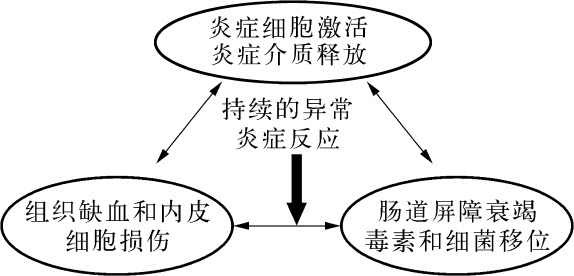
\includegraphics[width=.8\textwidth]{./images/Image00002.jpg}
	\caption{心肌萎缩}
	\label{fig1-1}
\end{figure}
%\FloatBarrier

萎缩的机制尚未完全搞清,蛋白合成少于分解可能为主要原因。

萎缩的器官、组织、细胞功能常降低,但一般是可复性的。原因消除后,萎缩的器官也可恢复正常。如原因持续存在,萎缩的实质细胞最后消失,间质结缔组织和脂肪细胞可以增生,甚至造成器官和组织体积增大,此时称假性肥大。

\subsection{肥大}

由于功能增加、合成代谢旺盛,细胞体积增大,使该器官、组织体积增大,称为肥大(hypertrophy)。肥大多发生于无分裂增殖能力或增殖能力较弱的细胞,如心肌、骨骼肌等。一般可分为生理性肥大和病理性肥大两类。如举重运动员上臂和胸部肌肉的粗壮肥大,妊娠子宫平滑肌细胞肥大属生理性肥大。病理情况下,也可发生肥大。例如高血压病,左心功能负荷加重,心肌纤维体积增大,一侧肾切除后另一侧肾体积增大,皆属代偿性肥大。而成人脑垂体前叶嗜酸细胞瘤分泌过多生长激素,导致的肢端肥大症,则属内分泌性肥大。肥大的细胞除了体积增大外,其内细胞器和微丝明显增多,蛋白合成旺盛。

有时实质细胞萎缩,间质增生也可使该器官、组织体积增大,这种假性肥大与前述的真性肥大有本质的区别。

\subsection{增生}

实质细胞数量增多,使该组织、器官体积增大,称为增生(hyperplasia)。增生可分为生理性和病理性增生两类。妇女在青春期、妊娠期和哺乳期乳腺上皮增生属生理性增生。病理情况下,例如溶血性贫血时骨髓的红细胞系增生,长期缺碘引起甲状腺组织增生,慢性鼻炎黏膜增生肥厚形成息肉等属于病理性增生。由于引起细胞、组织和器官增生与肥大的原因往往十分相似或相同,故两者常同时出现。这种现象见于雌激素过多时引起的子宫内膜增生、乳腺增生,以及老年男性因雄激素代谢障碍导致的前列腺增生。

\subsection{化生}

化生(metaplasia)是指一种已分化成熟的细胞由于适应环境改变而被另一种分化成熟细胞所代替的过程。化生并不是由一种成熟的细胞直接转变为另一种成熟的细胞,而是由该处具有分裂增殖和多向分化能力的幼稚细胞增生,向另一种类型的细胞分化、成熟,也就是所谓的异向分化,是环境因素引起细胞某些基因活化或受到抑制而重新编程表达的结果。化生常发生于同源细胞间,如一种上皮细胞与另一种上皮细胞间。化生是一种可复性病变,原因去除后大多可恢复。常见的化生有:

\subsubsection{鳞状上皮化生}

慢性支气管炎或长期吸烟者,气管及支气管的纤毛上皮转变为鳞状上皮。慢性胆囊炎及胆石症时,胆囊黏膜上皮发生鳞状上皮化生。慢性宫颈炎、子宫内膜炎时,黏膜上皮发生鳞状化生,在妇产科极为常见(图\ref{fig1-2})。肾盂结石时,肾盂黏膜的移行上皮也可转变为鳞状上皮。
\begin{figure}[!htbp]
	\centering
	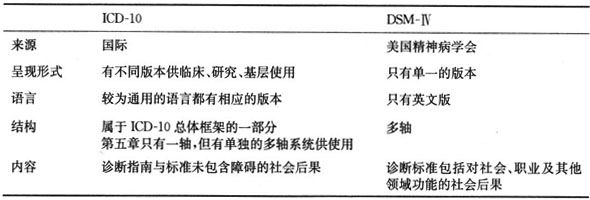
\includegraphics{./images/Image00003.jpg}
	\caption{子宫内膜鳞状上皮化生(HE染色,高倍) \\ {\small 子宫内膜的纤毛柱状上皮化生为鳞状上皮}}
	\label{fig1-2}
\end{figure}
%\FloatBarrier

\begin{framed}
	{案例1-1}

	{【病例摘要】}

	患者,男,55岁,因醉酒后呕吐、误吸,呛咳、呼吸困难入院。全麻下行支气管镜检查,从右主支气管中取出少量未消化米粒和菜叶,症状缓解;术中发现支气管黏膜充血、粗糙,征得家属同意后,夹取2块黏膜组织送病理检查。患者有吸烟史30年,反复咳嗽、咳痰史10年,否认其他病史。病理报告为“送检组织为少量鳞状上皮及其下疏松结缔组织、腺体,伴小血管充血和淋巴细胞、浆细胞浸润。符合慢性支气管炎。”

	{【问题】}

	(1)该患者支气管黏膜出现鳞状上皮,此属何种病理现象?

	(2)试分析病变形成机制和意义。
\end{framed}

\subsubsection{肠上皮化生}

慢性胃炎时,部分胃黏膜上皮转变为含有杯状细胞、潘氏细胞及具有纹状缘的吸收上皮,与小肠黏膜上皮相似;或在柱状上皮中,间有杯状细胞,与大肠黏膜上皮相似,均称为肠上皮化生(简称肠化)。类似的化生也常发生于腺体,由一种腺上皮转变为另一种腺上皮,故又称腺性化生。

\subsubsection{结缔组织和支持组织化生}

纤维组织化生为脂肪组织或肌细胞,成纤维细胞转变为骨母细胞或软骨母细胞,分别化生为骨或软骨(图\ref{fig1-3})。
\begin{figure}[!htbp]
	\centering
	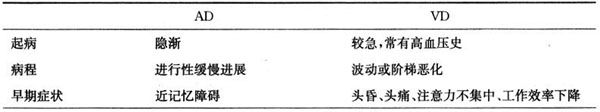
\includegraphics{./images/Image00004.jpg}
	\caption{心瓣膜软骨化生(HE染色,高倍) \\ {\small 心瓣膜结缔组织出现软骨化生}}
	\label{fig1-3}
\end{figure}
%\FloatBarrier

\begin{center}
	\textbf{知识链接}
\end{center}
\chapterabstract{上皮间质转分化(epithelial-mesenchymal
transition)为近年研究热点,其实也是一种化生现象。它是指上皮细胞在某些因素刺激下,逐渐失去上皮细胞表型(如E钙黏蛋白、细胞骨架蛋白等的表达)而呈现间质细胞表型(如波形蛋白、平滑肌肌动蛋白、纤维连接蛋白等的表达)。该现象可见于多种生理病理过程,如胚胎发育、组织重塑、肿瘤侵袭转移、慢性炎症和器官纤维化等。}

化生是机体对环境中不良因子发生防御反应的一种形式,对机体是有利的,但也有其局限性和不完善性。例如支气管黏膜鳞状化生后,失去纤毛,削弱了黏膜的自净能力。在化生、增生的基础上,还可能发展为肿瘤。例如支气管鳞状上皮化生和胃黏膜肠上皮化生,分别与肺鳞状细胞癌和胃腺癌的发生有一定的关系。

综上所述,组织细胞为了适应内外环境的变化,可出现萎缩、肥大、增生和化生等形态学改变(图\ref{fig1-4})。若刺激因素使发育正常的组织或器官内实质细胞体积缩小或数目减少即称为萎缩;实质细胞体积增大,即称为肥大;实质细胞数量增多,即称为增生;已分化成熟的细胞被另一种分化成熟细胞所代替即称为化生。

\begin{figure}[!htbp]
	\centering
	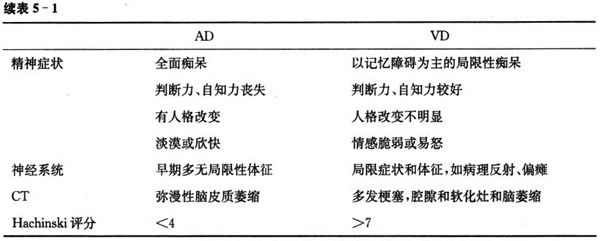
\includegraphics{./images/Image00005.jpg}
	\caption{四种适应性改变示意图}
	\label{fig1-4}
\end{figure}
%\FloatBarrier

\section{细胞和组织的损伤}

当损伤因素超出机体的适应能力,则引起细胞和组织的损伤。在一定程度内这种损伤为可复性,形态上表现为变性和物质异常沉积。重度损伤则引起细胞和组织的死亡。

\subsection{细胞和组织损伤的原因与发生机制}

\subsubsection{缺氧}

缺氧是引起组织细胞损伤常见而重要的原因。缺氧常见于:各种原因造成动脉供血不足或静脉回流障碍,或由于呼吸、循环障碍使血氧含量不足,也可见于严重贫血或中毒(如CO中毒)使红细胞携氧能力降低等情况。缺氧首先影响细胞的需氧呼吸,即线粒体的氧化磷酸化功能,使ATP产生减少或停止,导致细胞膜的钠泵功能障碍,Na{+}
及水在细胞内集聚,K{+}
从细胞外溢,造成急性细胞肿胀。缺氧也使无氧酵解过程增强,通过糖原分解产生ATP,以维持细胞的能量,但在无氧酵解的过程中细胞内乳酸、酮体、氨基酸和无机酸等氧化不全的代谢产物大量积聚,使pH下降。随之粗面内质网核蛋白体脱失、裂解,并出现线粒体肿胀,内质网扩张等一系列超微结构改变。以上改变是可复性的,随缺氧的恢复而恢复正常。如缺氧持续存在,ATP供应耗竭,细胞酶系统广泛损伤,细胞膜功能严重受损,细胞外Ca{2+}
不断进入细胞内,甚至进入线粒体内,使其基质中出现无定形的富于钙的致密区,线粒体发生不可复性改变,以至参与代谢的某些酶活性受抑,并使蛋白变性,细胞死亡。细胞内pH进一步下降将导致溶酶体膜的损伤,其内多种酶进入细胞浆内并被激活,其中酸性水解酶可引起细胞自溶死亡。

不同组织细胞对缺氧的耐受程度不同。结缔组织对缺氧耐受时间最长,而神经细胞对氧极为敏感,缺氧长于5~10分钟,细胞则发生不可复性损伤。

\subsubsection{物理因子}

物理因子包括机械性、高温、低温、电流、放射线等刺激因子。机械性损伤能使细胞组织破裂;高温使细胞内蛋白质(包括酶)变性,低温可使血管收缩引起组织缺血性损伤,或造成局部血流停滞、凝血,甚至细胞内水分形成冰晶而损伤细胞;电流通过组织时引起高温灼伤局部组织;放射线作用于机体能直接或间接造成大分子损伤,使水分被激发电离,产生大量具有强毒力的自由基,损伤组织细胞。物理因子引起损伤的严重程度主要决定于该物理因子的作用性质、强度和持续时间的长短,而很少和机体的反应性有关。

\subsubsection{化学因子}

许多化学物质进入人体,在组织细胞内发生化学反应,可破坏正常的生理功能。化学物质造成组织损伤前提是它们必须能经口、呼吸道、皮肤或黏膜进入体内才能引起中毒。化学因子引起损伤的机制是多方面的:①直接损伤:如强酸、强碱可直接灼伤皮肤或黏膜,引起局部炎症或坏死;②抑制酶的活性:如有机磷农药能抑制胆碱酯酶的活性,引起损伤。氯化汞和体内的巯基结合,从而使许多酶蛋白失去活性或破坏膜蛋白结构;③通过代谢形成毒性代谢产物而发挥作用:例如,四氯化碳经肝细胞滑面内质网所含的细胞色素P-450混合功能氧化酶类的作用,裂解生成毒性物质CCl{3}
和Cl自由基,后者可引起肝细胞发生脂肪变性和坏死。

自由基(free
radical)又称游离基,是指一类含有未配对电子的化学基团,如H{+} 、OH{-}
、HOO、O{2-}
,其化学活性高而不稳定,它与细胞内各种有机或无机化合物,如脂质、蛋白质、核酸等,发生过氧化、交联或断裂,从而造成细胞的损伤。但在正常人体内,自由基在细胞外液中的浓度极低,不构成对细胞的威胁,而在吞噬细胞杀灭病原生物或抗肿瘤细胞过程中自由基却起重要防御作用。但是如果体内生成过多,或清除障碍,如在上述的化学性、放射性、炎症损伤过程中,或随着年龄的增长,机体抗氧化活性递减,逐级降低对自由基的防御能力,均可引起组织细胞损伤或机体衰老。自由基可在正常新陈代谢中产生,是普遍存在于生物系统的代谢中间产物,种类多,数量大,活性高。

\subsubsection{生物性因子}

生物性因子是引起细胞损伤最常见的原因,包括病毒、细菌、立克氏体、真菌、寄生虫等引起的各种感染。其作用机制有下列几方面:①直接作用损伤细胞和组织:病毒寄生于细胞内干扰细胞的代谢活动,使细胞变性坏死。②通过内外毒素的作用或产生的毒性代谢产物:如白喉外毒素自由基能抑制细胞的氧化过程和蛋白质的合成。溶血性链球菌产生的透明质酸酶和链激酶引起间质损伤。③生物因子具有抗原性,能引起变态反应:肝炎病毒有嗜肝细胞的特性并产生病毒蛋白,后者可通过变态反应引起肝细胞损伤。

\subsubsection{免疫反应}

免疫反应是机体的正常防御功能,通过免疫反应排斥异己物质,以维持内环境的稳定。但这种反应结果并非均对机体有利,例如病毒性肝炎,在机体T细胞致敏清除肝炎病毒的过程中也造成肝细胞的损伤;在某些情况下对病原生物产生的抗体与体内组织抗原发生交叉反应,形成抗原抗体复合物沉积于组织,引起损伤,如风湿性心肌炎,急性肾小球肾炎,通过变态反应对自身组织抗原发生反应,引起组织细胞的损伤;甚至针对自身组织发生自身免疫反应,如红斑性狼疮,类风湿关节炎等。

\subsubsection{其他}

遗传缺陷、营养失衡、内分泌异常、衰老、心理和社会因素等也能导致组织细胞的损伤。

综上所述,引起组织细胞损伤的因子很多,它们主要通过以下几个途径造成细胞损伤(图\ref{fig1-5}):①ATP耗竭,细胞需要能量的生理活动受阻;②细胞膜完整性破坏、渗透性缺陷,导致细胞内容物流失或物质交换和电生理活动异常;③细胞内钙离子浓度升高,多种酶被激活,使ATP耗竭或细胞结构的破坏;④自由基产生增多;⑤其他代谢活动异常等。一种因子可通过多种途径损伤细胞,几种因子亦可共用一条途径使细胞受累。
\begin{figure}[!htbp]
	\centering
	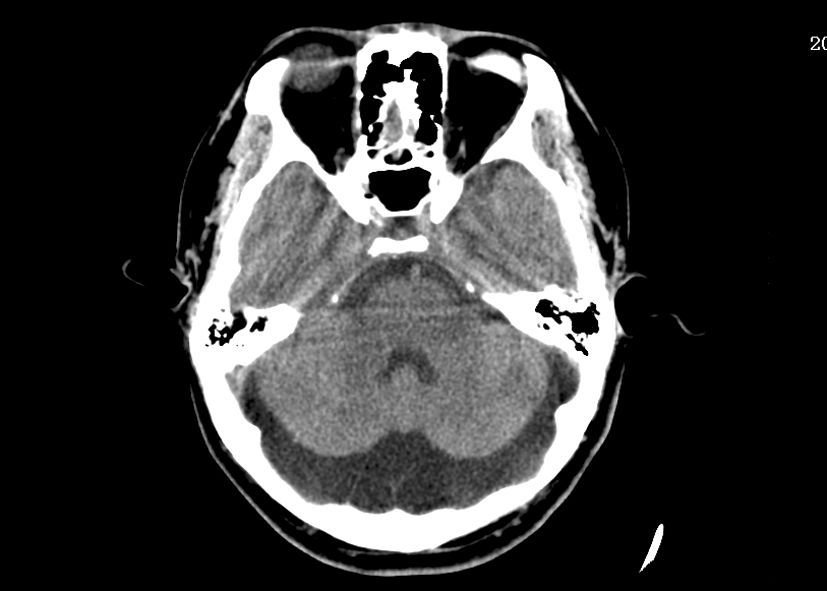
\includegraphics{./images/Image00006.jpg}
	\caption{组织细胞损伤机制示意图}
	\label{fig1-5}
\end{figure}
%\FloatBarrier 

\subsection{细胞和组织损伤的形态学变化}

组织细胞损伤有轻重之别,损伤因子强度弱、作用时间短,细胞的损伤可恢复,即为可逆性损伤;若损伤因子持续刺激和过于剧烈,细胞将会死亡,则表现为不可逆性损伤。

\subsubsection{可逆性损伤}

可逆性损伤(reversible
injury),旧称变性(degeneration),是指新陈代谢障碍时,细胞或细胞间质内出现一些异常物质或正常物质异常蓄积。变性的组织细胞功能下降,但通常为可复性,严重者可发展为坏死。变性的种类繁多,下面介绍比较常见的几种变性。

\paragraph{细胞水肿}
细胞水肿(cellular edema)或称水变性(hydropic
degeneration)即细胞内水钠积聚过多,引起细胞体积肿大,胞浆疏松、透明淡染。常见于缺氧、感染、中毒时的心、肝、肾等脏器的实质细胞。

病理上,轻度的细胞水肿,胞浆内出现许多细小的伊红染颗粒,此乃水肿时肿大的线粒体和扩张的内质网,这种变化致相应器官肉眼观时体积轻度增大,包膜紧张,颜色较正常淡,显得混浊而无光泽,在电镜技术问世之前称之为颗粒变性(granular
degeneration)或混浊肿胀,此名词现已弃用。随细胞内水钠积聚增多,细胞水肿进一步发展,线粒体和内质网高度扩张,囊泡变,此时镜下观:胞浆透明、空泡状,故又有空泡变性或水样变性之称(图\ref{fig1-6})。病毒性肝炎和四氯化碳中毒时,肝细胞水肿,严重者细胞肿大如圆球状,特称为气球样变(图\ref{fig1-7})。
\begin{figure}[!htbp]
	\centering
	\begin{minipage}[b]{0.45\textwidth}
		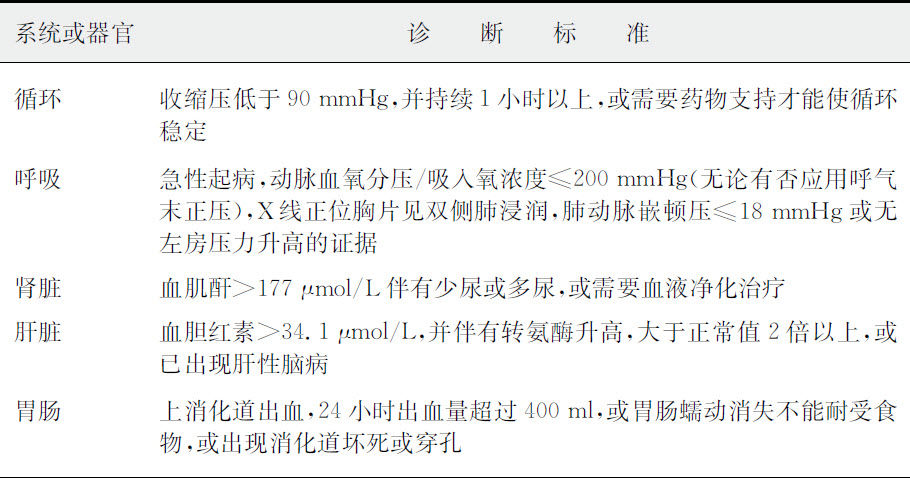
\includegraphics{./images/Image00007.jpg}
		\caption{肾小管上皮细胞水肿(HE染色,高倍) \\ {\small 细胞体积增大,胞浆内出现红染的颗粒状物}}
		\label{fig1-6}
	\end{minipage}
	%	\end{figure} 
	%\FloatBarrier
	%\begin{figure}[!htbp]
	%    \centering
	\hspace{0.04\textwidth}%
	\begin{minipage}[b]{0.45\textwidth}
		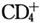
\includegraphics{./images/Image00008.jpg}
		\caption{肝细胞水肿(HE染色,中倍) \\ {\small 肝细胞明显肿胀,细胞浆疏松}}
		\label{fig1-7}
	\end{minipage}
\end{figure}
%\FloatBarrier

引起细胞水肿的原因很多,在急性感染、缺氧、中毒等有害因素的作用下,线粒体产能机制受损,ATP生成减少,使细胞膜的钠泵功能障碍,导致细胞内水、钠增加,细胞水肿。或由于细胞膜直接受损,通透性增高所致。

细胞水肿是一种轻度或中度损伤的表现,在原因消除后,仍可恢复正常。若病因持续存在,水肿细胞的胞浆内可出现脂滴空泡。严重水肿可引起细胞坏死。

\paragraph{脂肪变性}
除脂肪细胞外,其他细胞胞浆内出现脂滴或脂滴明显增多称为脂肪变性(fatty
degeneration),简称脂变。脂变常发生于心、肝、肾等代谢旺盛或耗氧较多的器官。脂变中的脂滴,主要成分为中性脂肪,也可有磷脂及胆固醇等成分,在常规石蜡包埋的切片中,中性脂肪被制片过程中所使用的乙醇、二甲苯等脂溶剂溶解,所以HE染色的切片,光镜下细胞中的脂滴呈空泡状。在冰冻切片苏丹Ⅲ染色时显示脂肪滴为橘红色,锇酸染色时呈黑色。

(1)肝脂肪变性:由于肝脏在脂肪代谢中起重要作用,故肝脂变最多见,且常较严重。肉眼观:轻度脂变时肝脏无明显改变,脂变广泛时肝脏均匀性肿大,包膜紧张,边缘钝,色淡黄,切面有油腻感,苏丹Ⅲ染色后变成红色(图\ref{fig1-8}a)。镜下观:HE染色切片可见早期脂变表现为核周围出现小的脂肪空泡,以后渐增大,散布于胞浆中,严重时融合成一个大空泡,将核推挤到包膜下,状似脂肪细胞(图\ref{fig1-8}b)。脂变在肝小叶内的分布与病因有一定的关系。如肝淤血时,小叶中央区淤血明显,缺氧较重,脂变首先发生于此处。长期淤血,小叶周边区肝细胞也因缺氧而发生脂变,而小叶中央区的肝细胞大多已萎缩或消失。磷中毒时,脂变主要发生在小叶周边区,可能与该区肝细胞代谢较为活跃,对磷中毒更为敏感所致。此外,小叶周边的肝细胞接触到的毒物浓度较高也使此处的肝细胞易受损伤。
\begin{figure}[!htbp]
	\centering
	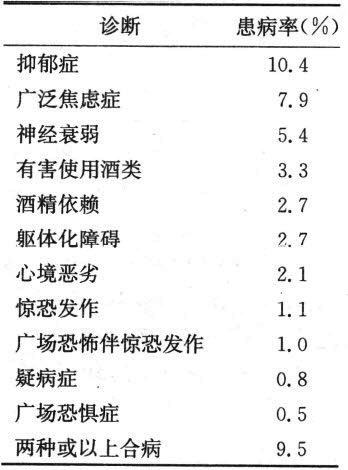
\includegraphics{./images/Image00009.jpg}
	\caption{肝脂肪变性}
	\label{fig1-8}
\end{figure}
%\FloatBarrier 



肝脂变是可复性损伤,病因消除后,脂变细胞可恢复正常,一般无明显的临床表现。重度弥漫性肝脂变称为脂肪肝,体检时肝可在右季肋下触及,常规B超可进行诊断。病变持续发展,肝细胞逐渐坏死,纤维组织增生,可发展为肝硬化。

(2)心肌脂肪变性:多见于贫血。肉眼观:轻度脂变一般无明显异常,但在严重贫血时,常在心内膜下,尤其是左心室乳头肌处出现红黄相间的条纹,如虎皮斑纹,称为“虎斑心”。这是由于心肌内血管分布不均,心肌缺氧轻重程度不一所致,血管末梢分布区心肌缺氧较重,脂变明显而呈黄色,缺氧较轻部位脂变较轻,心肌呈红色。镜下观:脂肪空泡常较细小,呈串珠状排列。有时心外膜增生的脂肪组织可沿间质深入心肌细胞间,称为心肌脂肪浸润(图\ref{fig1-9})。
\begin{figure}[!htbp]
	\centering
	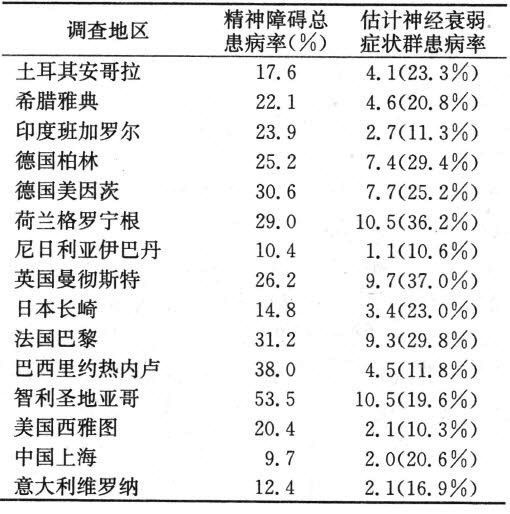
\includegraphics[width=0.7\textwidth]{./images/Image00010.jpg}
	\caption{心外膜脂肪组织增生及心肌脂肪浸润}
	\label{fig1-9}
\end{figure}
%\FloatBarrier 

(3)肾脂肪变性:贫血、缺氧、中毒和一些肾脏疾病时,肾曲管上皮细胞可发生脂肪变性。这是因为在上述疾病时肾小球毛细血管通透性增加,肾曲管特别是近曲小管上皮吸收漏出的脂蛋白,在细胞内分解成脂滴。脂滴空泡多位于近曲小管上皮细胞基底部或核周围。

脂肪变性发生的机制尚未完全清楚。一般认为与感染、中毒、缺氧等因素干扰或破坏细胞的脂肪代谢有关。具体作用途径则因病因不同而异。肝脂变的机制大致如下:①脂蛋白合成障碍,使脂肪堆积在肝细胞内不能转运出去。其原因常是缺乏合成脂蛋白的原料,如磷脂或组成磷脂的胆碱,或由于化学物或其他毒素破坏了内质网(蛋白合成部位)或抑制了某些酶的活性,使脂蛋白合成障碍。②脂肪酸氧化障碍。由于缺氧、感染、中毒,使线粒体受损,干扰β-氧化,使肝细胞含脂肪量增加。③进入肝细胞脂肪酸过多。例如饥饿或某些疾病造成饥饿状态,或糖尿病患者对糖的利用障碍,机体动用大量体脂,其中大部分以脂肪酸的形式进入肝脏,超过肝细胞将其氧化和合成脂蛋白的能力,于是在肝细胞内储积。

\paragraph{玻璃样变性}
玻璃样变性(hyaline
degeneration)又称透明变性,是指在HE染色情况下,细胞外间质或细胞质内出现伊红染、均质半透明、无结构的玻璃样物质。玻璃样变性其实为一组物理性状相同,但其发生原因、化学成分及机制各不相同的病理变化的统称。常见的玻璃样变性有三类:

(1)细胞内玻璃样变性:指细胞浆内出现大小不等、圆形、均质的红染小滴。细胞内玻璃样变性可由多种原因引起,如肾小球肾炎或其他疾病伴有明显蛋白尿时,肾近曲小管上皮细胞胞浆内可出现大小不等的圆形红染小滴,这是血浆蛋白经肾小球滤出而又被肾小管上皮细胞吞饮、融合而成的玻璃样小滴(图\ref{fig1-10}a)。慢性乙醇中毒时,由于细胞中间丝前角蛋白变性,肝细胞核周围的胞浆内可出现圆形或形状不甚规则的均质红染玻璃样物质,称为Mallory小体。

(2)结缔组织玻璃样变性:常发生在增生的纤维结缔组织,为胶原纤维老化的表现。肉眼观病变处呈灰白色,半透明,质地致密而坚韧(图\ref{fig1-10}b)。光镜下胶原蛋白交联、变性、融合,胶原纤维增粗并互相融合成索带状或片状的半透明均质物,纤维细胞明显减少。见于瘢痕组织、纤维化的肾小球、动脉粥样硬化的纤维斑块等。

(3)血管壁玻璃样变性:常发生于高血压病时的肾、脑、脾及视网膜的细动脉。这是由于细动脉持续痉挛,使内膜通透性增大,血浆蛋白渗入内膜,在内皮细胞下凝固成均匀红染玻璃样物质。如病变继续发展,血管壁平滑肌组织均被玻璃样物质替代而消失,再加上基底膜样物质增多,使病变血管壁增厚、变硬,管腔狭窄甚至闭塞,此即细动脉硬化症(图\ref{fig1-10}c),可引起肾、脑等器官缺血。
\begin{figure}[!htbp]
	\centering
	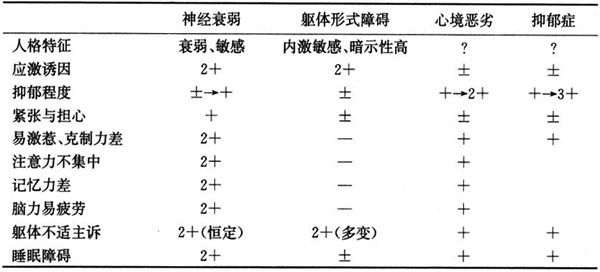
\includegraphics[width=0.7\textwidth]{./images/Image00011.jpg}
	\caption{不同类型玻璃样变性}
	\label{fig1-10}
\end{figure}
%\FloatBarrier

上述3种类型中,细胞内玻璃样变在病因去除后多能恢复,而后两者较难恢复。

\paragraph{黏液样变性}
组织间质内出现类黏液(黏多糖和蛋白质)的积聚称为黏液样变性(mucoid
degeneration)。镜下观:病变处细胞间质疏松,充以淡蓝色的胶状液体,其间散布一些多角形,星芒状的细胞,并以突起互相连缀。黏液样变性常见于间叶性肿瘤、急性风湿病时的心血管壁、动脉粥样硬化的血管壁。在甲状腺功能低下时,透明质酸酶活性受抑,含有透明质酸的黏液样物质及水分在皮下蓄积,形成黏液水肿。

\paragraph{淀粉样变}
组织内有淀粉样物质沉着称为淀粉样变(amyloid
degeneration)。淀粉样物质是蛋白质,其遇碘时可被染成棕褐色,再加硫酸后则变为蓝色,与淀粉染色特性相似,故称之为淀粉样变。此种病变可见于慢性炎症、内分泌系统肿瘤、老年性痴呆(Alzheimer病)等多种疾病。淀粉样物质的沉积可为局部性,亦可为全身性,常分布于细胞间或沉积在小血管基底膜下,还可沿组织纤维支架分布。镜下观:淀粉样物质呈淡伊红染色、均匀一致、云雾状。刚果红染色为橘红色(图\ref{fig1-11})。尽管形态相似,但在不同疾病时,淀粉样物质的化学本质不同,有的为免疫球蛋白,有的为激素,还有的为β{2}
淀粉样蛋白,等等。

\begin{figure}[!htbp]
	\centering
	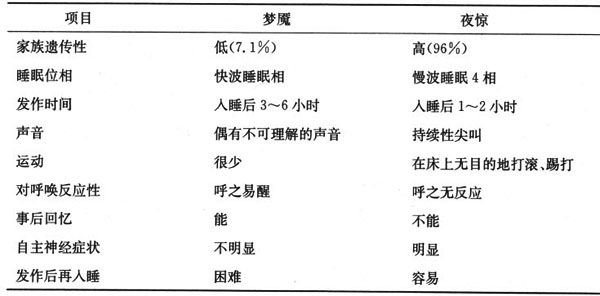
\includegraphics[width=0.7\textwidth]{./images/Image00012.jpg}
	\caption{肾小球淀粉样变}
	\label{fig1-11}
\end{figure}
%\FloatBarrier

\paragraph{病理性色素沉积}
细胞或组织内可有各种来自体内、体外的色素沉积,在病理情况下某些色素在体内会过量沉积。常见的病理性色素沉积有含铁血黄素、胆红素、脂褐素、黑色素。

(1)含铁血黄素(hemosiderin):系由铁蛋白微粒积聚而成的色素,颗粒状,棕黄或金黄色,具有折光性。此色素为血红蛋白被吞噬细胞溶酶体分解而成,如巨噬细胞破裂,则色素逸出于间质中。正常的骨髓组织或脾内可有少量含铁血黄素出现,在全身溶血性疾病时,含铁血黄素可沉积在全身的单核巨噬细胞系统内,组织出血时含铁血黄素常出现在出血灶附近。当左心衰竭导致肺淤血时,红细胞自肺泡壁毛细血管漏出于肺泡中,被巨噬细胞吞噬,肺泡腔内可出现吞噬含铁血黄素的巨噬细胞,又称为心力衰竭细胞。

(2)胆红素(bilirubin):也是在巨噬细胞内形成的一种血红蛋白衍生物,棕黄色或黄绿色。生理情况下,胆红素是衰老的红细胞被单核吞噬细胞分解后所形成。血中胆红素过多时,可将组织和体液染成黄色,称黄疸。因有血脑屏障,胆红素通常不能进入脑和脊髓,但在新生儿由于血脑屏障尚不完善,溶血性黄疸时,大量胆红素可进入脑细胞内,使其氧化磷酸化过程受损,能量产生受抑制,导致细胞变性,出现相应的神经症状。肉眼见豆状核、下丘脑、海马回等多处神经核明显黄染,故称之为核黄疸。胆红素一般呈溶解状态,但在胆道阻塞及某些肝脏疾病时也可为黄褐色折光性颗粒或团块,出现于肝细胞、Kupffer细胞、毛细胆管、小胆管等组织细胞内。

(3)脂褐素(lipofuscin):为一种黄褐色细颗粒状色素。其组成成分的50%为脂质,其余为蛋白质及其他物质。脂褐素系细胞内自噬溶酶体中的细胞器碎片发生了某种理化改变,不能被溶酶体酶消化而形成的一种不溶性残存小体。老年人及一些慢性消耗性疾病患者的肝细胞、肾上腺皮质网状带细胞和心肌细胞核两端的胞浆中可见到脂褐素,故又有消耗性色素之称。

(4)黑色素(melanin):为棕褐色或黑褐色的颗粒状色素,大小形状不一。正常人黑色素多存在于皮肤、毛发、虹膜及脉络膜的黑色素细胞内。它是由酪氨酸在黑色素细胞内的酪氨酸酶的作用下氧化、聚合而形成的一种不溶性聚合体。人脑垂体所分泌的ACTH能刺激黑色素细胞,促进黑色素形成。在肾上腺皮质功能低下时,对垂体的反馈抑制作用减弱,致使ACTH分泌增多,患者全身皮肤黑色素增多。局部黑色素增多常见于黑色素痣或恶性黑色素瘤等。

\paragraph{病理性钙化}
在病理情况下,骨和牙以外的组织内有固体钙盐的沉积,称为病理性钙化(pathologic
calcification)。主要成分为磷酸钙、碳酸钙及少量铁镁等物质。肉眼观:少量钙盐沉积难以辨认,仅在刀切组织时有砂粒感;量多时表现为白色石灰样颗粒或团块,质地坚硬。镜下观:HE染色切片中,钙盐呈蓝色颗粒状。病理性钙化可分为两种类型:

(1)营养不良性钙化:指钙盐沉积于变性、坏死的组织中或异物内,如结核坏死灶、脂肪坏死灶、动脉粥样硬化斑块的变性坏死区(图\ref{fig1-12}a),血栓、寄生虫体和虫卵。患者无全身钙、磷代谢障碍,血钙不高。这是一种较常见的病理性钙化,可能与局部碱性磷酸酶(来自坏死细胞及其周围组织内)升高有关。

\begin{figure}[!htbp]
	\centering
	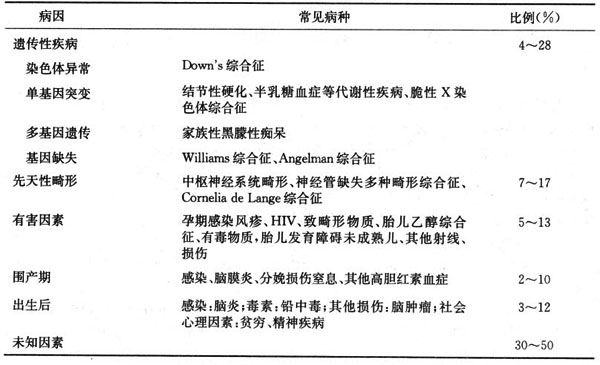
\includegraphics[width=0.7\textwidth]{./images/Image00013.jpg}
	\caption{动脉壁钙化}
	\label{fig1-12}
\end{figure}
%\FloatBarrier

(2)转移性钙化:较少见,是指由于全身钙、磷代谢障碍,血钙和(或)血磷升高,钙盐沉积于未受损的组织中。如甲状腺功能亢进或骨肿瘤造成骨组织破坏时,大量骨钙进入血液,使血钙升高,并沉积于肾小管、肺泡、胃黏膜和动脉壁中层(图\ref{fig1-12}b)。接受超剂量维生素D时,由于肠道对钙磷吸收明显增加,也可引起钙化。

钙化对机体的影响视具体情况而异。坏死组织钙化常是病灶愈合的表现,而血管壁的钙化则使管壁失去弹性、变硬、变脆,容易破裂出血。转移性钙化的危害性主要决定于原发病。

\subsubsection{不可逆性损伤-细胞死亡}

当细胞发生不可逆性代谢、结构和功能障碍,则引起细胞死亡(cell
death)。细胞死亡是病理学核心问题,其表现有两种方式:坏死与凋亡。坏死是细胞受到严重损伤时的病理性死亡过程,而凋亡多属生理性情况下发生的死亡,由细胞基因编程调控,在某些病理情况下,细胞死亡也可以凋亡形式出现。

\paragraph{坏死}
坏死(necrosis)是细胞受到严重损伤,以酶溶性变化为特点的活体内局部组织细胞的死亡。坏死可迅速发生,但在多数情况下由可逆性损伤逐渐发展而来。基本表现为细胞肿胀、细胞器崩解和蛋白质变性。

(1)坏死的基本病变

1)细胞核的改变:这是细胞坏死在形态学上的主要标志,表现为:①核浓缩(pyknosis),由于核脱水使染色质浓缩,嗜碱性染色增强,核体积缩小。②核碎裂(karyorrhexis),核染色质崩解为小碎片,核膜破裂,染色质碎片分散在胞质中。③核溶解(karyolysis),在DNA酶的作用下,染色质DNA分解,核乃失去对碱性染料的亲和力,因而染色变淡,仅见核轮廓,最后核消失(图\ref{fig1-13})。

\begin{figure}[!htbp]
	\centering
	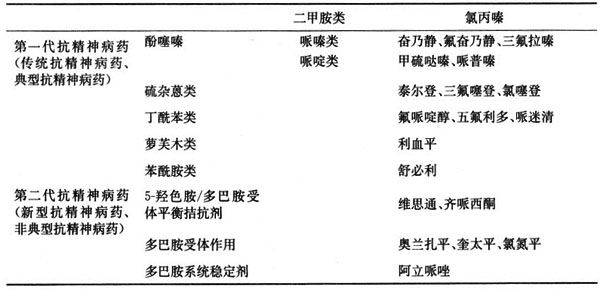
\includegraphics[width=0.7\textwidth]{./images/Image00014.jpg}
	\caption{细胞坏死时核的变化}
	\label{fig1-13}
\end{figure}

2)细胞浆的改变:由于细胞浆内嗜碱性核蛋白体减少或丧失,胞质变性蛋白质增多、糖原颗粒减少,使胞质对碱性染料苏木素的亲和力减少,而与酸性染料伊红的亲和力增强,致胞浆红染,坏死后期细胞浆崩解。

3)间质的改变:在实质细胞坏死后一段时间内,间质常无改变,以后在溶解酶的作用下,基质崩解,胶原纤维肿胀、断裂,继而崩解、液化。最后坏死的实质细胞和间质融合成一片无结构的颗粒状、红染物质,其内有时可见少量淡染的细胞核碎片。

由于坏死时细胞膜通透性增加,细胞内乳酸脱氢酶、琥珀酸脱氢酶、肌酸激酶、门冬氨酸氨基转移酶、丙氨酸氨基转移酶等被释放入血,造成细胞内酶活性降低而血浆中相应的酶活性升高,分别可作为诊断某些细胞(如肝、心肌、胰)坏死的参考指标。细胞内和血浆中酶活性的变化在坏死初即可检出,有助于细胞损伤早期诊断。

(2)坏死的病理类型:组织坏死后,由于酶的分解和蛋白质变性等因素综合作用的结果,使坏死组织出现不同的形态学变化,总体上可分为凝固性坏死、液化性坏死和特殊类型坏死等三个基本类型。

1)凝固性坏死(coagulation
necrosis):组织坏死后,蛋白质变性凝固且溶酶体酶水解作用较弱时,坏死区呈灰黄、干燥、质实状态,称为凝固性坏死。这种坏死多由缺血引起,常在心、肾、脾等器官的缺血性坏死时出现。
坏死灶周围常有暗红色出血带,与健康组织分界(图\ref{fig1-14}a)。
镜下特点:早期坏死灶细胞微细结构消失,但细胞组织的结构轮廓仍可保留一段时间(图\ref{fig1-14}b)。
最终坏死细胞崩解成碎片,被吞噬细胞吞噬或被游走进入的白细胞释放的溶解酶溶解。
凝固性坏死的发生机制仍不很清楚,可能是组织坏死后蛋白变性过程占优势,而水解酶的作用较少。

\begin{figure}[!htbp]
	\centering
	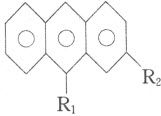
\includegraphics[width=.7\textwidth]{./images/Image00015.jpg}
	\caption{凝固性坏死}
	\label{fig1-14}
\end{figure}

2)液化性坏死(liquefaction
necrosis):组织坏死后分解、液化而呈液体状,有时还形成含有液体的腔。
如脑组织,坏死后分解成半流体状物质,又称为脑软化。
这种变化与脑组织水分和磷脂含量多,蛋白质含量少有关,故组织坏死后不易凝固而液化。
在某些病原体如化脓性细菌或溶组织阿米巴原虫能释放或产生蛋白溶解酶,可使组织发生液化性坏死。

3)特殊类型坏死

①干酪样坏死(caseous
necrosis):结核病时,坏死区内脂质较多,颜色带黄,质地松软,状似干酪,故称为干酪样坏死。
镜下观:坏死组织分解比较彻底,原有组织轮廓消失,呈现为一片红染、无定形的颗粒状物质(图\ref{fig1-15})。
梅毒性的坏死组织具有相似的形态,但其中的弹力纤维及血管结构仍可保留,致使坏死组织质地坚韧如树胶,故名树胶肿。
干酪样坏死不易吸收,一旦形成将存留较长时间。

\begin{figure}[!htbp]
	\centering
	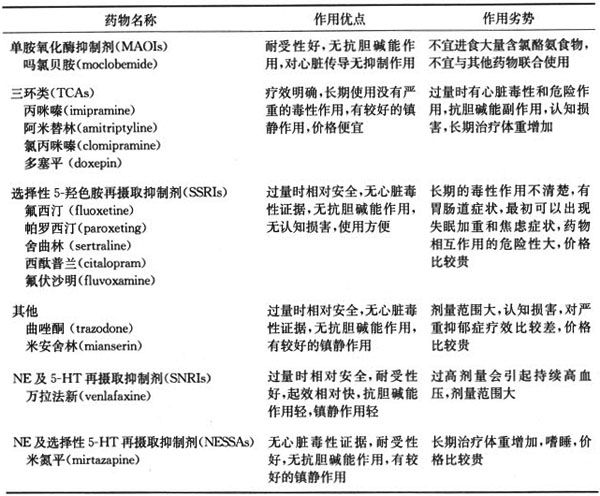
\includegraphics{./images/Image00016.jpg}
	\caption{肾干酪样坏死 \\ {\small 肾剖面可见多个黄白色干酪样坏死灶。}}
	\label{fig1-15}
\end{figure}

②纤维素样坏死(fibrinoid necrosis):旧称纤维素样变性(fibrinoid
degeneration)为发生于结缔组织胶原纤维和小血管壁的一种坏死。病变部位组织结构逐渐消失,变为一片境界不清的颗粒状、小条状或小块状无结构物质,经伊红染成深红色,由于其与纤维素染色性质相似,故名。常见于风湿病、结节性多动脉炎、新月体性肾小球肾炎、系统性红斑性狼疮等变态反应性疾病(图\ref{fig1-16})。也可见于恶性高血压病时的细动脉和胃溃疡底部动脉壁。其发生机制与抗原-抗体复合物引发的胶原纤维肿胀崩解、结缔组织免疫球蛋白沉积或血液纤维蛋白渗出变性有关。

\begin{figure}[!htbp]
	\centering
	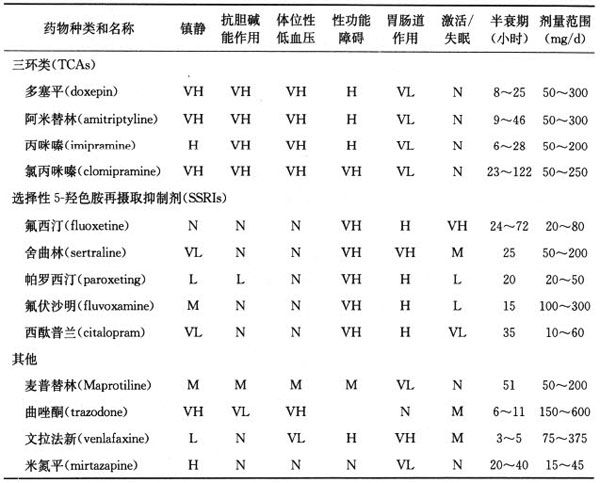
\includegraphics{./images/Image00017.jpg}
	\caption{肾小动脉壁纤维素样坏死(HE染色,高倍) \\ {\small 箭头所示深伊红染区为小动脉壁纤维素样坏死。}}
	\label{fig1-16}
\end{figure}


③脂肪坏死(fatty
necrosis):为液化性坏死的一种特殊类型,又可分为酶解性脂肪坏死和外伤性脂肪坏死。
前者常见于急性胰腺炎,由于胰脂酶外逸并被激活,对胰腺自身及腹腔的脂肪组织发生分解作用,形成的脂肪酸与组织内钙盐结合,在大网膜、后腹壁及肠系膜表面形成灰白色、质硬的不透明斑点或斑块,称为皂钙。
外伤性脂肪坏死常发生于富于脂肪组织的部位,乳腺尤其多见,有外伤史,局部表现为增大的肿块。镜下为大量的泡沫细胞及异物巨细胞。

④坏疽(gangrene):大块组织坏死后继发腐败菌感染,出现不同程度的腐败性变化。
腐败菌在分解坏死组织的过程中产生大量的硫化氢,并与血红蛋白分解释出的铁离子结合,形成硫化亚铁,致使坏死组织臭而发黑。
根据坏疽发生的部位、原因及形态特征不同,可分为干性、湿性、气性等类型。
干性坏疽(dry
gangrene)多发生于动脉阻塞而静脉回流仍然通畅的四肢末梢,坏死局部干燥、皱缩,呈黑色,与周围组织分界清楚(图\ref{fig1-17}),腐败性变化较轻。
湿性坏疽(moist
gangrene)常发生于与体外相连的内脏,如肠、阑尾等器官,也可发生于四肢。
形成的原因除动脉阻塞外,同时伴有局部淤血,坏死组织含水量多,适合腐败菌生长。
坏死区局部明显肿胀,呈深黄、暗绿或污黑,与周围组织无明显分界线,可引起严重的全身中毒症状。气性坏疽(gas
gangrene)也属于湿性坏疽。系深达肌肉的开放性创伤合并产气荚膜杆菌、腐败弧菌等厌氧菌感染。
细菌在分解液化组织的过程中产生大量气体,使坏死组织呈蜂窝状,压之有捻发感。
病变发展迅猛,沿肌束迅速蔓延。由于大量毒素被吸收,患者中毒症状十分严重,常需要紧急处理。

\begin{figure}[!htbp]
	\centering
	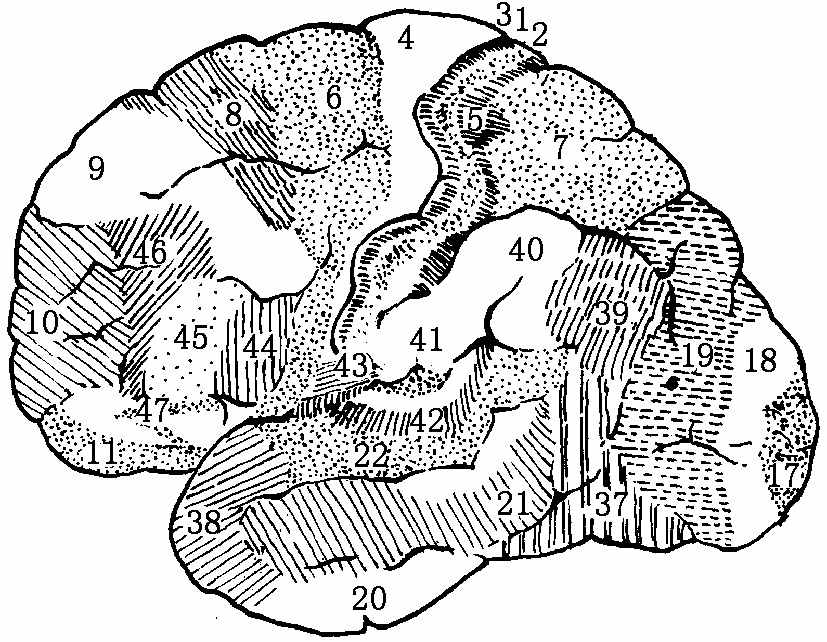
\includegraphics{./images/Image00018.jpg}
	\caption{足(干性)坏疽}
	\label{fig1-17}
\end{figure}

(3)坏死的结局:组织坏死后成了机体的异物,刺激周围组织,引起局部反应。不同的坏死组织结局不尽相同。

1)溶解吸收:坏死细胞自身或周围的炎细胞释放的溶解酶将坏死组织分解、液化,然后由淋巴管或小血管吸收,未被完全分解的组织碎片由吞噬细胞吞噬清除。坏死范围较大可形成囊腔。留下的组织缺损通过再生修复,这是机体处理坏死组织的基本方式。

2)分离排出:较大的坏死灶不易完全吸收,由于其周围发生炎症反应,其中的白细胞释放的溶解酶加速周边坏死组织溶解、吸收,使坏死灶与健康组织分离。位于皮肤、黏膜的坏死组织分离后脱落,留下局部缺损,浅者称为糜烂,深者称为溃疡。肾和肺脏的坏死组织分离后经自然管道排出,留下的空腔称为空洞。

3)机化与纤维包裹:坏死组织如不能被溶解吸收或分离排出,则由周围新生的毛细血管和成纤维细胞(合称肉芽组织)逐渐长入,取代坏死组织,最后形成瘢痕组织。这种由肉芽组织取代坏死组织(或其他异物、血凝块、血栓及渗出物等)的过程称为机化(organization)。如果坏死灶较大,难以吸收、机化,周边部增生的肉芽组织可将坏死灶包围,尔后肉芽组织转变为纤维组织,称为纤维包裹。机化和包裹的肉芽组织最终形成纤维瘢痕。

4)钙化:坏死组织和细胞碎片若未被及时清除,则日后易发生钙盐及其他矿物质沉积,引起营养不良性钙化。陈旧性干酪样坏死病灶或坏死的脂肪组织常有明显的钙化。

\paragraph{细胞凋亡}
细胞凋亡(apoptosis)也称程序性细胞死亡,是真核细胞在一定条件下通过启动其自身内部机制,主要是激活内源性核酸内切酶而发生的细胞主动性死亡方式。与细胞坏死不同,凋亡是一种主动过程,通常为单个细胞或小灶性细胞死亡,而不是大片实质细胞同时死亡。凋亡细胞周围无炎症反应,故有人借用希腊词“apoptosis”来形容其像秋天枯萎的树叶,从树干上悄无声息地飘零下来。

(1)形态特征:凋亡细胞有独特的形态特征。早期表现为细胞变圆,微绒毛及细胞突起消失,同时胞质浓缩,内质网扩张呈泡状,并与细胞膜融合形成细胞质小泡,向外隆起但无膜破裂;核染色质浓缩、凝聚于核膜下呈半月形。而后细胞膜内陷,自行分割为数个由胞膜包裹的、表面光滑的凋亡小体,其中含有大小不等的染色质片断、结构尚保持完整的细胞器和胞质成分(图\ref{fig1-18})。凋亡小体可与周围细胞分离,很快被邻近的细胞或巨噬细胞吞噬,在胞质溶酶体内迅速降解。

\begin{figure}[!htbp]
	\centering
	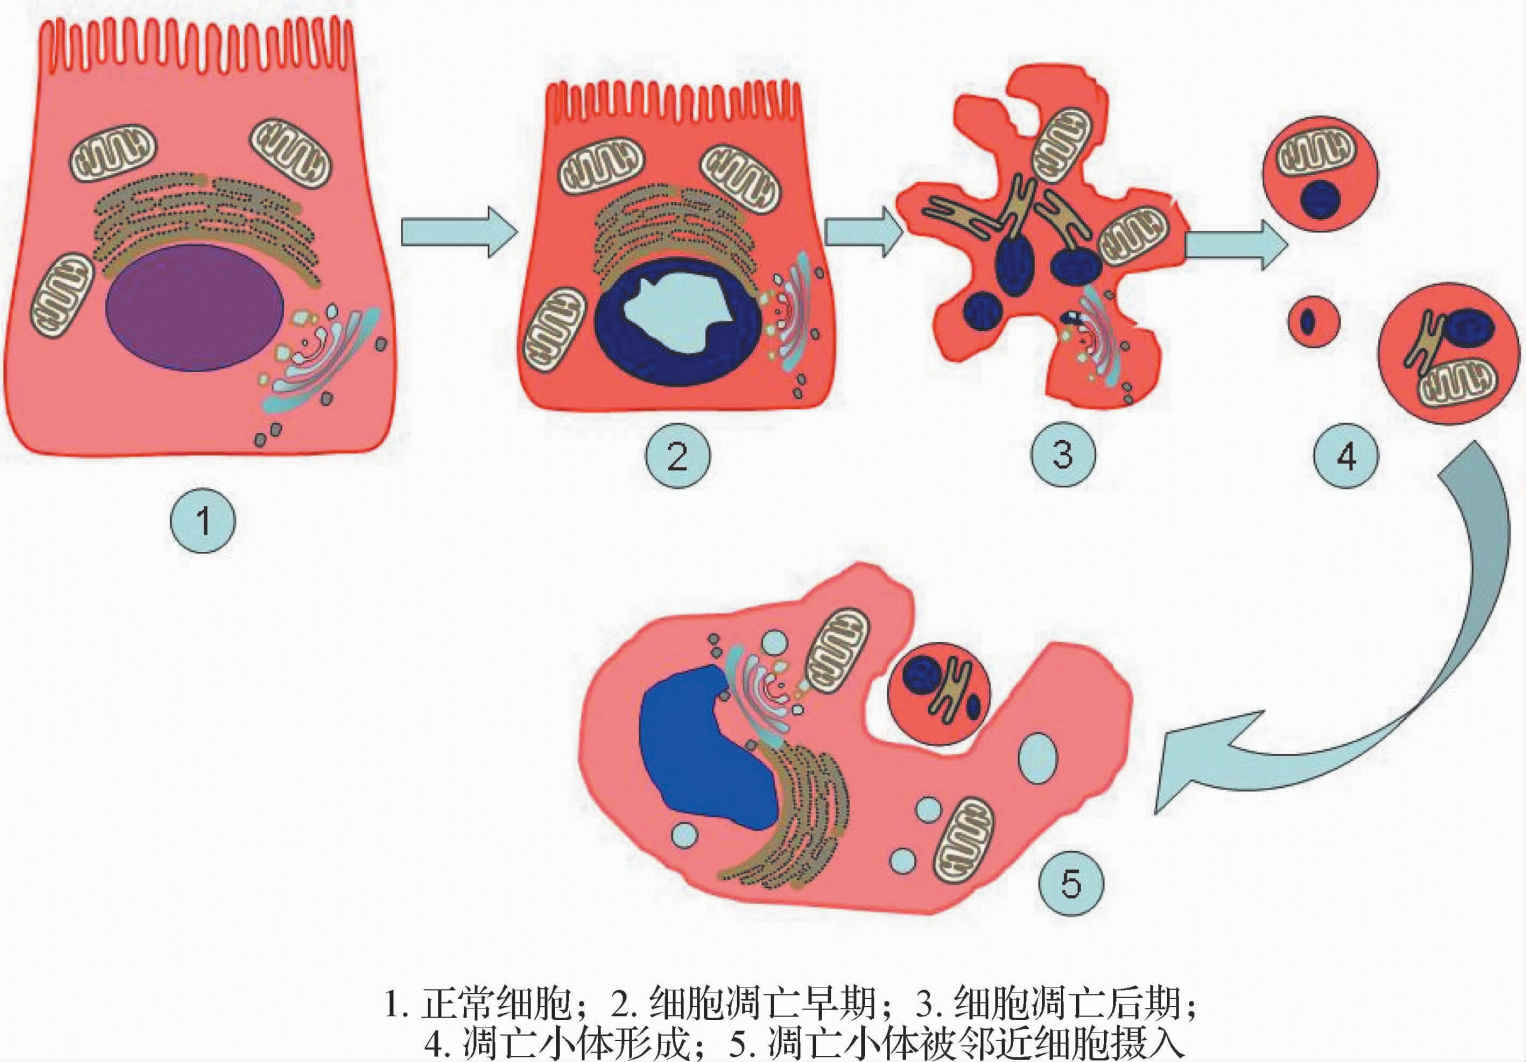
\includegraphics[width=.7\textwidth]{./images/Image00019.jpg}
	\caption{凋亡示意图}
	\label{fig1-18}
\end{figure}

(2)发生机制:细胞凋亡的发生机制十分复杂,它是一种由某些刺激因子启动、内在基因调控,并依赖能源的连锁分子事件,其中有信号传导、特异性调节分子作用、共同蛋白酶(caspases,半胱氨酸天冬氨酸蛋白酶,亦称胱冬肽酶)家族活化及死亡细胞的被噬和移去等过程,故曾有程序性死亡(programmed
cell death)之称。

刺激因子不同,其信号通路、调节分子种类不尽相同。目前已知,在人体各种病理过程中,发生细胞凋亡的主要通路有两条(图\ref{fig1-19}):一是线粒体通路或内源通路;二是死亡受体通路或外源通路。

\begin{figure}[!htbp]
	\centering
	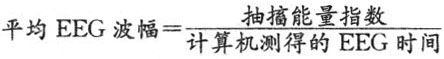
\includegraphics[width=.7\textwidth]{./images/Image00020.jpg}
	\caption{细胞凋亡机制示意图}
	\label{fig1-19}
\end{figure}

线粒体通透性决定细胞是否凋亡,而通透性受控于含20个以上蛋白成员的Bcl-2家族。当细胞失去生长因子或生存信号、暴露于DNA损伤因子(如紫外线、放射线、活性氧和细胞毒药物等)以及细胞内堆积过多的错误折叠蛋白时,Bcl-2家族感应分子即被活化,继之活化该家族另外两个成员(效应分子)-Bax和Bak,它们形成二聚体并插入线粒体膜,使后者通透性增加,细胞色素C和其他蛋白分子逸出线粒体进入胞浆,令激发性胱冬肽酶(caspase
9)活化,后者再使效应性胱冬肽酶(caspase
3、6、7)活化,最终导致细胞骨架蛋白崩解、核酸内切酶活化和凋亡小体形成。Bcl-2、Bcl-x{L}
抑制Bax和Bak活化,故可阻断凋亡。

细胞凋亡的死亡受体通路涉及肿瘤坏死因子(TNF)及其受体(TNFR)、FAS-FAS配体作用等。受体的胞内段为死亡功能区(dead
domain)。一旦受体配体结合,死亡信号即通过死亡功能区和相关的适配蛋白(adapter
protein)传递至激发性胱冬肽酶(caspase
8),并使之活化。后续反应与线粒体通路相同。

(3)细胞凋亡与坏死的区别:细胞凋亡的发生机制与前述的坏死不同,有相关基因调节。其中Fas、Bax、P53等基因有促进作用,Bcl-2、Bcl-x{L}
等有抑制凋亡作用。凋亡细胞内源性Ca{2+} 、Mg{2+}
依赖DNA内切酶的激活,从而切割核小体间DNA,形成不连续的180~200
bp或其倍数的DNA片断。被切割的DNA片断在琼脂糖凝胶电泳时表现为阶梯状电泳条带,这种现象被认为是细胞凋亡的可靠指标。凋亡的细胞质膜完整,无细胞内容物溢出,不引起细胞周围炎症反应,也不诱发周围细胞的增生修复。细胞凋亡和细胞坏死的区别见表\ref{tab1-1}。

\begin{table}[ht]
	\caption{细胞凋亡和细胞坏死的区别}
	\label{tab1-1}
	\centering
	\begin{tabular}{lp{5cm}p{5cm}}
		\toprule
		         & 细胞凋亡                                                                           & 细胞坏死                       \\
		\midrule
		形态特征 & 细胞固缩,核染色质边集、细胞膜及各细胞器膜完整,膜可发泡出芽,形成调亡小体
		         & 细胞显著肿胀,核染色质絮状或边集,细胞膜及各细胞器膜溶解破裂,溶酶体释放,细胞溶解                                  \\
		生化特征 & 核酸内切酶活化,半胱氨酸蛋白酶活化,谷氨酰谷氨酰转移酶活性增高
		         & 核酸内切酶无活化,半胱氨酸蛋白酶、转移酶活性无变化                                                                  \\
		DNA电泳  & 阶梯状条带                                                                         & 弥散分布的电泳拖带             \\
		炎症反应 & 无                                                                                 & 有                             \\
		机制     & 由凋亡相关基因调控主动进行(自杀性)                                                 & 与基因调控无关被动进行(他杀性) \\
		发生条件 & 多为生理性                                                                         & 病理性                         \\
		\bottomrule
	\end{tabular}
\end{table}


(4)细胞凋亡的生理、病理意义:细胞凋亡是最基本的生物现象,是机体生存和发育的基础。大量研究材料显示它涉及生命活动中的许多领域,包括发育、生长、造血、免疫、肿瘤发生等。通过凋亡可以清除多余的、无用的细胞。胚胎发育过程中,一些遗迹如人胚的尾芽和鳃随发育定期消亡,就是通过凋亡的方式进行的。细胞凋亡也可作为机体的自身保护机制,以清除发育不正常及对机体有害的细胞,畸胎瘤就是未彻底凋亡的残留胚层结构存留所致。B和T细胞发育成熟过程中本该发生凋亡的细胞保留下来将形成自身抗原,导致自身免疫病;细胞凋亡的异常改变包括凋亡不足或凋亡过度都可引起一些疾病。T辅助细胞($\text{CD}^+_4$
)在人类免疫缺陷病毒(HIV)感染后,发生凋亡,从而导致获得性免疫缺陷病。细胞凋亡的调控失常与肿瘤的发生关系密切,当机体某个基因发生突变而导致凋亡信号下调凋亡不足时,可引起细胞异常增生而发生肿瘤。目前临床上已开始用药物或放射线来诱导肿瘤细胞凋亡以达到治疗肿瘤的目的。

\begin{center}
	\textbf{知识链接}
\end{center}
\chapterabstract{自噬(autophagy)是细胞对自身细胞器或胞内聚集的变性蛋白等大分子物质进行包裹以及降解消化的现象。近年发现自噬不足或过度均可导致细胞死亡,所以被称为第三种细胞死亡方式。}

生理状态下,细胞通过自噬来清除受损、衰老和失去功能的细胞器及各种大分子物质,最终降解产物再循环利用,为细胞重建和再生提供原料。病理状态下,自噬不仅能保护细胞免受毒物损伤,而且能抵御病原体的侵害。在机体的免疫、感染、炎症、肿瘤、心血管病和神经退行性疾病的发生发展过程中均发挥重要作用。自噬和凋亡有相似之处,如二者共享某些调节蛋白,如胱冬肽酶。某些刺激因素既可诱导自噬亦可引起凋亡。

总之,疾病源于组织细胞的损伤,内外因子的刺激强度不同,损伤程度不同(图\ref{fig1-20})。若刺激在细胞能承受范围内,则表现为适应,属轻度损伤,细胞可出现萎缩、增生、肥大和化生等形态学改变。若刺激时间长强度大,细胞将发生显著损伤,出现细胞内外异常物质沉积,甚至坏死;若刺激因素激活特殊信号系统,细胞可发生凋亡。

\begin{figure}[!htbp]
	\centering
	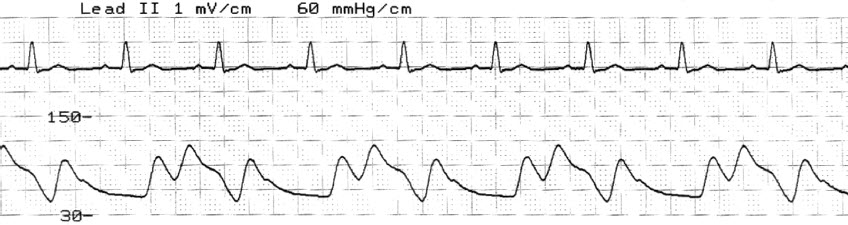
\includegraphics{./images/Image00023.jpg}
	\caption{组织细胞适应、损伤概览}
	\label{fig1-20}
\end{figure}

\section*{复习与思考}

{一、名词解释}

适应 萎缩 肠上皮化生 细胞水肿 脂肪变性 虎斑心 病理性钙化 凝固性坏死 干酪样坏死 液化性坏死 脑软化 坏疽 细胞凋亡

{二、问答题}

1. 机体组织细胞可出现哪几种适应性改变?

2. 久病卧床后肢体变细属于哪种类型的萎缩?为什么?

3. 试述肝脂变的原因和病变。

4. 何谓玻璃样变?好发于哪些部位?

5. 体内常见的色素有哪些?光镜下的特点是什么?

6. 试述坏死的镜下特点及结局。

7. 细胞的坏死和凋亡如何区别?


\chapter{免疫系统}
\begin{framed}
\noindent\textbf{【知识体系】}

\begin{center}
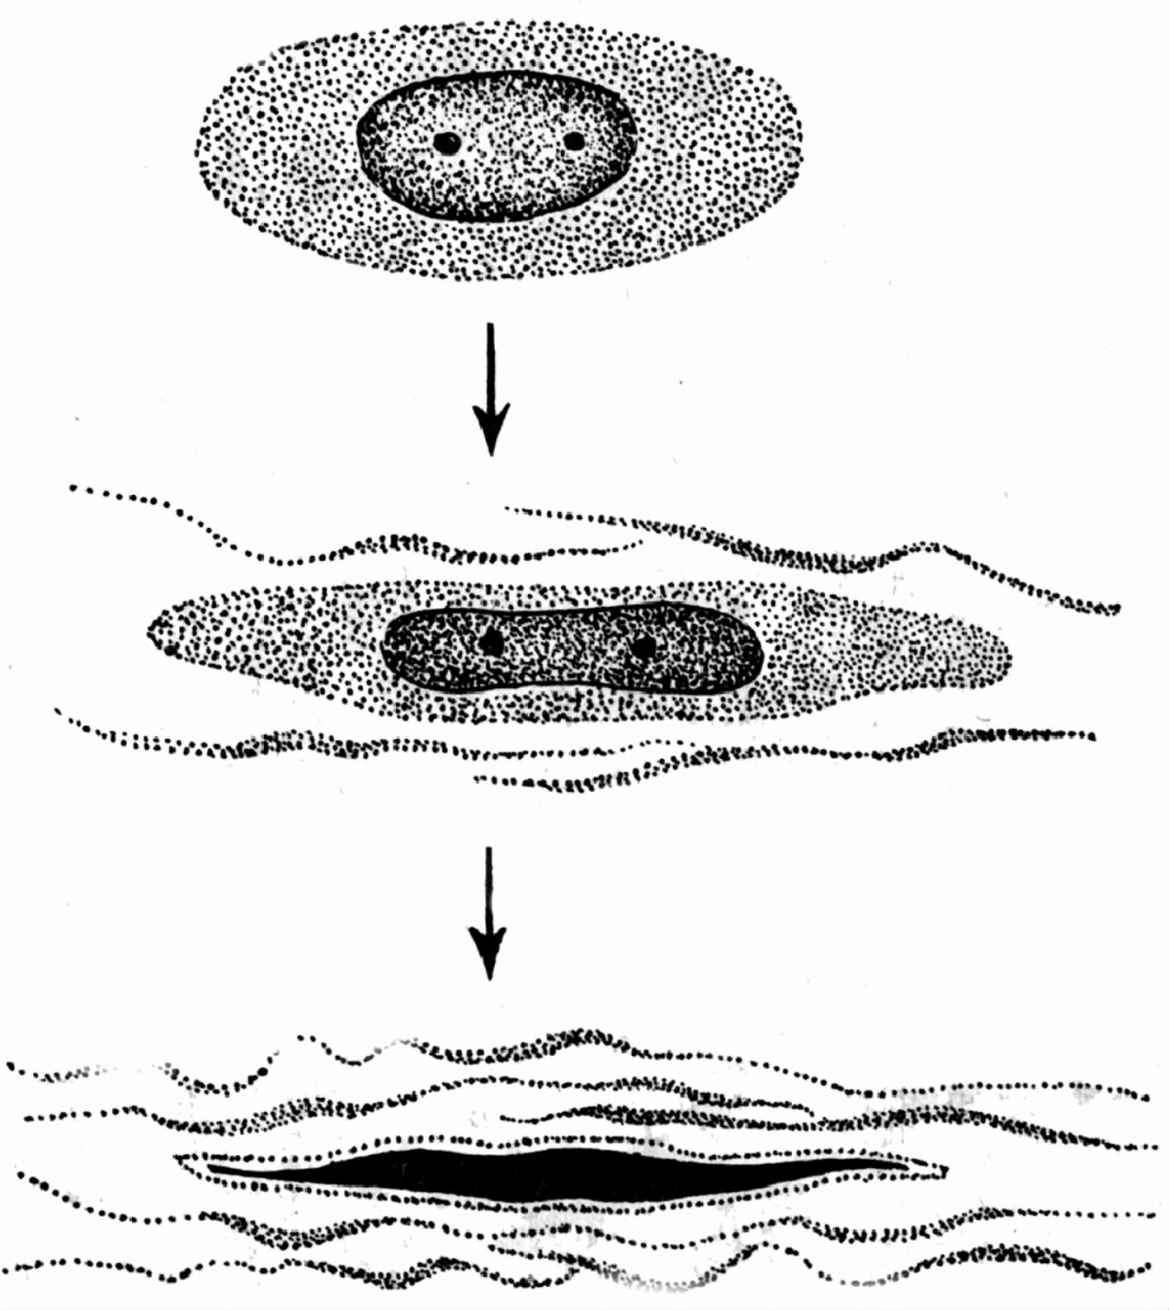
\includegraphics[width=.66\textwidth]{./images/Image00025.jpg}
\end{center}

\noindent\textbf{【课前思考】}

与机体的其他组织系统一样,免疫系统由哪些组织、器官、细胞组成?各种器官、细胞有何特征?在维护我们机体健康中各自起到怎样的作用?当有病原微生物入侵时,机体的各种免疫细胞是怎样各司其职又相互协调的?机体的免疫系统与国家的防御体系有何相似之处?

\noindent\textbf{【本章重点】}

1.免疫系统的构成;

2.免疫器官、免疫细胞的功能。

\noindent\textbf{【教学目标】}

1.掌握免疫系统组成:免疫器官(中枢免疫器官、外周免疫器官)、免疫细胞、免疫分子;

2.掌握中枢免疫器官的组成:骨髓、胸腺的主要免疫功能;

3.掌握外周免疫器官与组织的组成:淋巴结、脾脏的主要免疫功能。
\end{framed}
机体抵御外界病原微生物的入侵有三道防卫系统:

1.皮肤、黏膜及其分泌物

皮肤黏膜的机械阻挡作用和附属物(如纤毛)的清除作用,皮肤黏膜分泌物(如汗腺分泌的乳酸、胃黏膜分泌的胃酸等)的杀菌作用,体表和与外界相通的腔道中寄居的正常微生物丛对入侵微生物的拮抗作用等,属于机体第一道防线。其次是内部屏障。抗原物质一旦突破第一道防线进入机体后,即遭到机体内部屏障的清除,包括:淋巴和单核吞噬细胞系统屏障、正常体液中的一些非特异性杀菌物质、血脑屏障和胎盘屏障等(图\ref{fig2-1})。

\begin{figure}[!htbp]
 \centering
 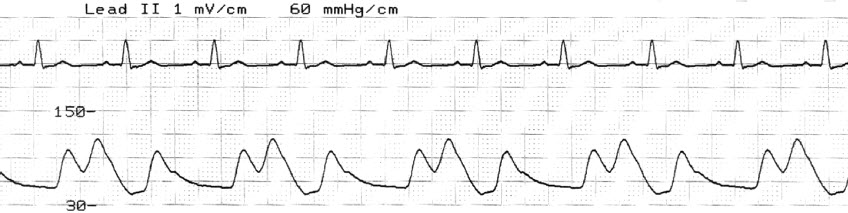
\includegraphics[width=.6\textwidth]{./images/Image00026.jpg}
 \caption{机体第一道防线}
 \label{fig2-1}
  \end{figure} 

2.吞噬细胞、NK细胞、抗菌蛋白、炎症应答------淋巴系统

微生物进入机体组织以后,多数沿组织细胞间隙的淋巴液经淋巴管到达淋巴结,但淋巴结内的巨噬细胞会消灭它们,阻止它们在机体内扩散,这就是淋巴屏障作用。如果微生物数量大、毒力强,就有可能冲破淋巴屏障,进入血液循环,扩散到组织器官中去。这时,它们会受到单核吞噬细胞系统屏障的阻挡。这是一类大的吞噬细胞。机体内还有一类较小的吞噬细胞,其中主要的是中性粒细胞和嗜酸性粒细胞。它们不属于单核吞噬细胞系统,但与单核吞噬细胞系统一样,分布于全身,对入侵的微生物和大分子物质有吞噬、消化和消除的作用。

在正常体液中的一些非特异性杀菌物质,如补体、调理素、溶菌酶、干扰素、乙型溶素、吞噬细胞杀菌素等,也与淋巴和单核吞噬细胞系统屏障一样,是机体的第二道防线,有助于消灭入侵的微生物(图\ref{fig2-2})。

\begin{figure}[!htbp]
 \centering
 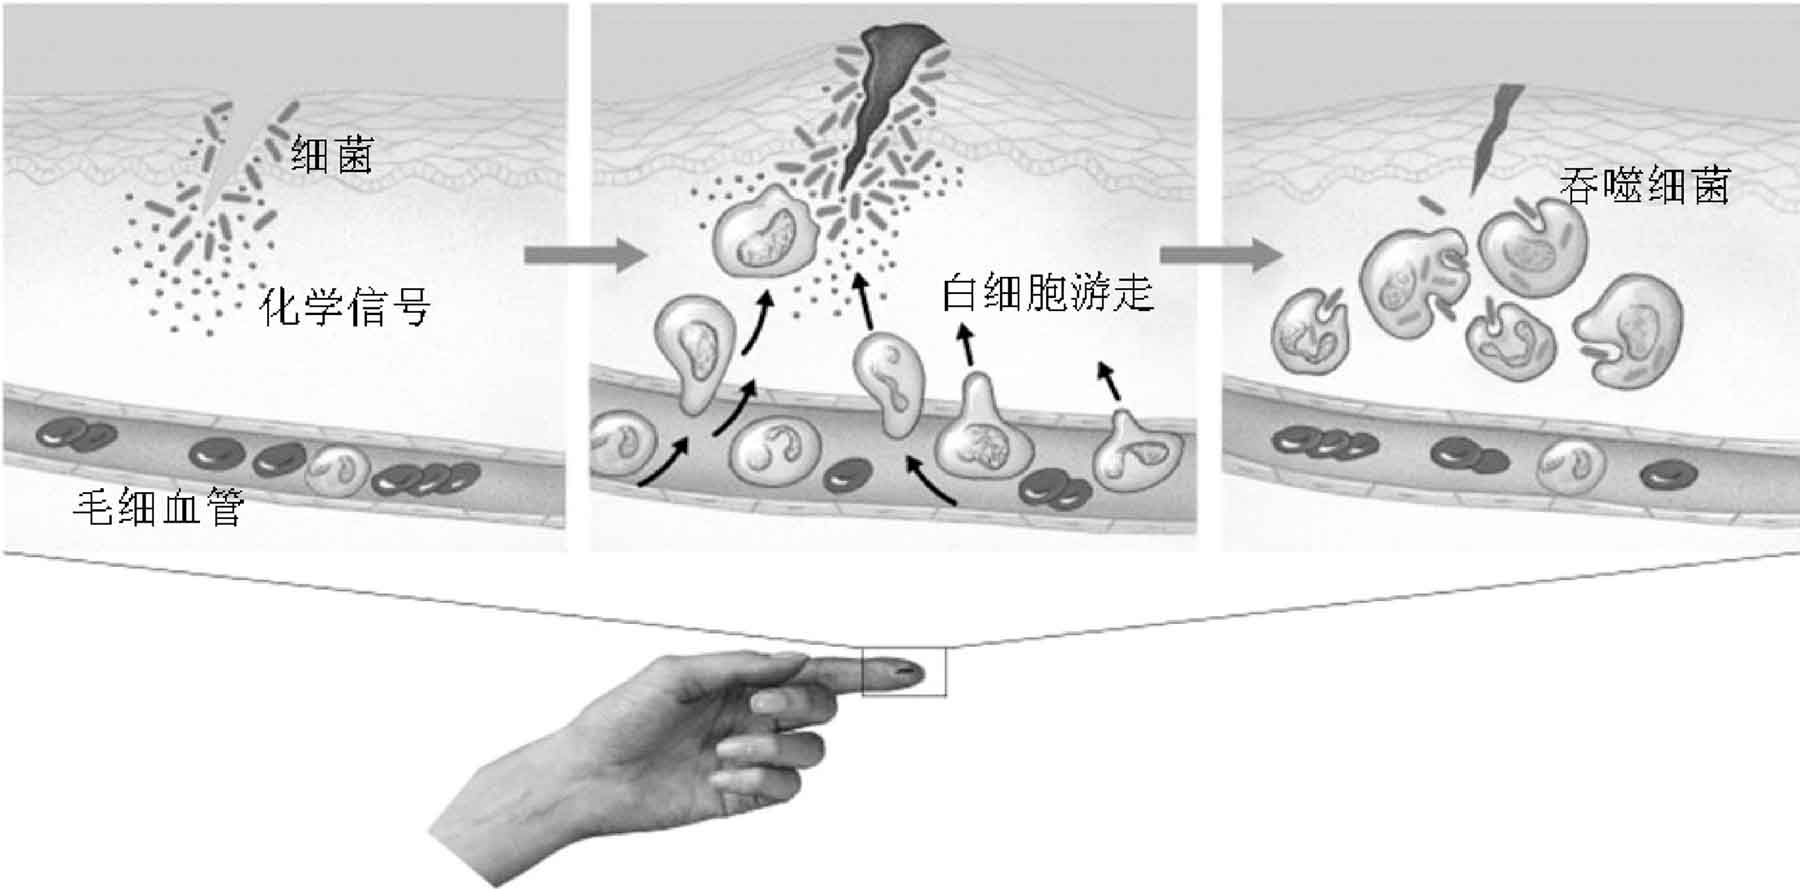
\includegraphics[width=.6\textwidth]{./images/Image00027.jpg}
 \caption{机体的第二道防线}
 \label{fig2-2}
  \end{figure} 

3.免疫系统:淋巴细胞、抗体;特点:特异性、多样性、记忆性、识别自我与非我(图\ref{fig2-3})。

\begin{figure}[!htbp]
 \centering
 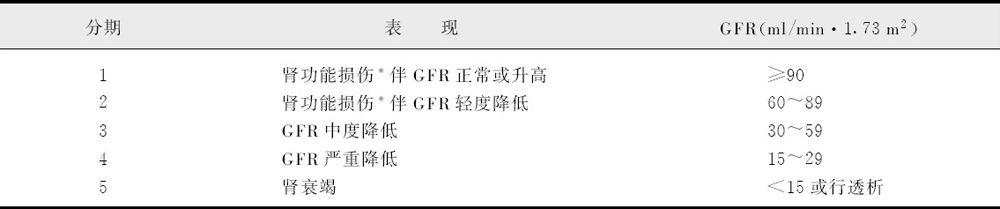
\includegraphics[width=.5\textwidth]{./images/Image00028.jpg}
 \caption{机体的第三道防线------免疫系统}
 \label{fig2-3}
  \end{figure} 

我们主要讲授免疫系统。

免疫系统(immune
system)乃承担免疫功能的组织系统,是机体对抗原刺激产生应答、执行免疫效应的物质基础。从宏观至微观进行描述,免疫系统包括免疫器官(中枢免疫器官和外周免疫器官)、免疫细胞(造血干细胞、淋巴细胞、单核吞噬细胞及其他免疫细胞)和免疫分子(抗体、补体、细胞因子)。

\section{中枢免疫器官}

中枢免疫器官(central immune
organ)是免疫细胞发生、分化、发育、成熟的场所,并对外周免疫器官的发育起主导作用,某些情况下(如再次抗原刺激或自身抗原刺激)也是产生免疫应答的场所。人和其他哺乳类动物的中枢免疫器官包括骨髓、胸腺,鸟类腔上囊(法氏囊)的功能相当于骨髓。


\subsection{骨髓}

骨髓(bone
marrow)是重要的中枢免疫器官,可分为红骨髓和白骨髓。红骨髓由结缔组织、血管、神经和实质细胞组成,呈海绵样存在于骨松质的腔隙中,具有活跃的造血功能。骨髓功能的发挥与其微环境有密切关系。骨髓微环境指造血细胞周围的微血管系统、末梢神经、网状细胞、基质细胞以及它们所表达的表面分子和所分泌的细胞因子。这些微环境组分是介导造血干细胞黏附、分化发育、参与淋巴细胞迁移和成熟的必需条件。骨髓是人和哺乳动物的造血器官(图\ref{fig2-4})。它具有如下功能:

1.各类免疫细胞发生的场所:骨髓造血干细胞具有分化成不同血细胞的能力,故被称为多能造血干细胞(multiple
hematopoietic stem
cell,HSC)。在骨髓微环境中,HSC首先分化为髓样前体细胞(myeloid
progenitor)和淋巴样前体细胞(lymphoid
progenitor)。髓样前体细胞最终分化成为粒细胞、单核细胞、红细胞、血小板;淋巴样前体细胞分化为T淋巴细胞(简称T细胞)、B淋巴细胞(简称B细胞)和自然杀伤细胞(NK细胞)。

\begin{figure}[!htbp]
 \centering
 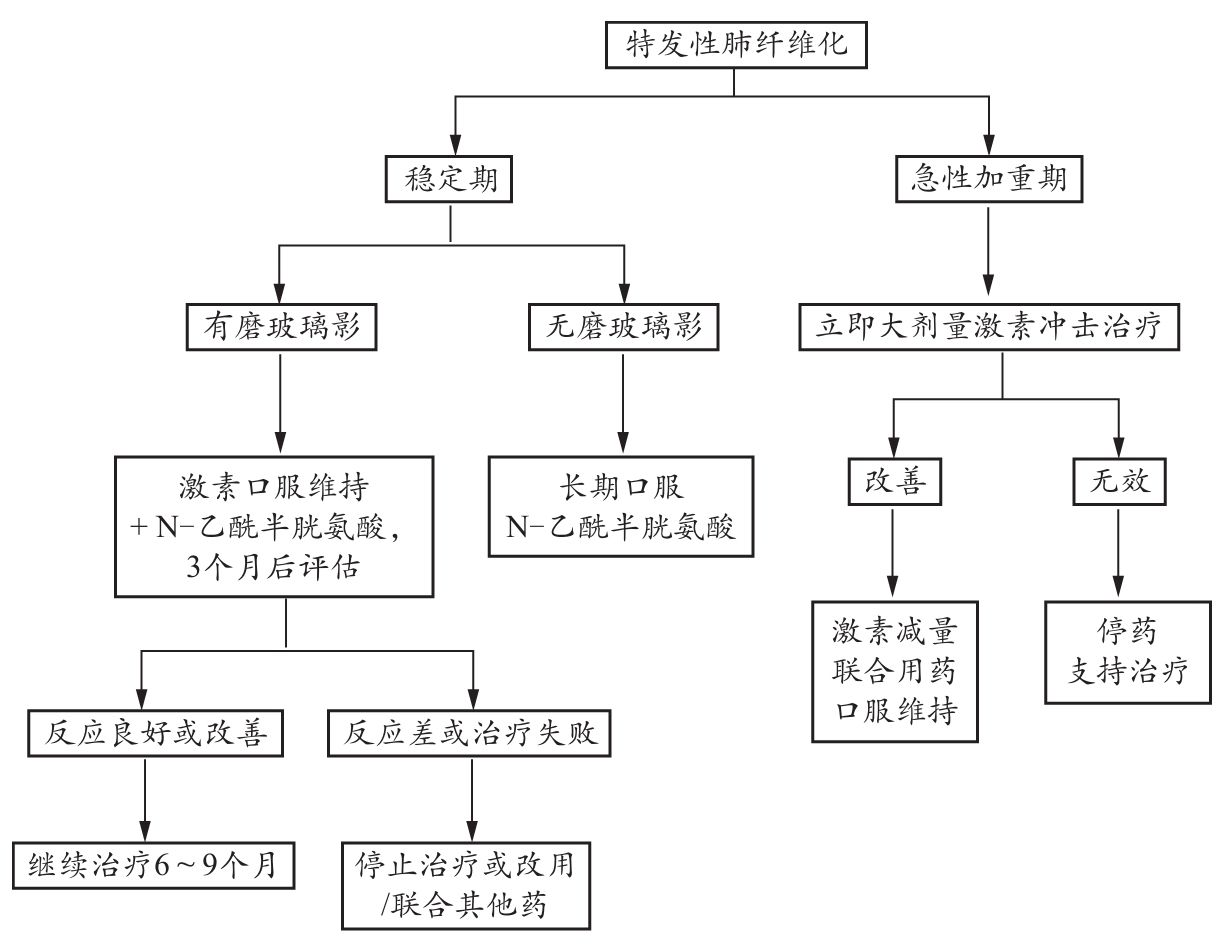
\includegraphics[width=.6\textwidth]{./images/Image00029.jpg}
 \caption{血细胞发育示意图}
 \label{fig2-4}
  \end{figure} 

2.B细胞分化成熟的场所:骨髓中产生的淋巴样前体细胞循不同的途径分化发育:一部分经血液迁入胸腺,发育成熟为成熟的T细胞;另一部分则在骨髓内继续分化为成熟B细胞。与T细胞在胸腺中分化的过程类似,B细胞在骨髓中也发生抗原受体(B
cell
receptor,BCR)等表面标志的表达、选择性发育或凋亡等。成熟的B细胞进入血循环,最终也定居在外周免疫器官。

3.发生B细胞应答的场所:骨髓是发生再次体液免疫应答的主要部位,外周免疫器官中的记忆性B细胞在抗原刺激下被活化,经淋巴液和血液进入骨髓后分化成熟为浆细胞,并产生大量抗体释放至血液循环。外周免疫器官中所发生的再次应答,其产生抗体的速度快,但持续时间短;而骨髓中所发生的再次应答,其产生抗体的速度慢,但可缓慢、持久地产生大量抗体,从而成为血清抗体的主要来源。

最新研究成果表明:在一定的微环境中,骨髓中的造血干细胞和基质干细胞还可分化为其他组织的多能干细胞(如神经干细胞、心肌干细胞等),这一突破性的进展开拓了骨髓生物学作用的全新领域,并可望在组织工程和临床医学中得到广泛应用。


\subsection{胸腺}

\begin{figure}[!htbp]
 \centering
 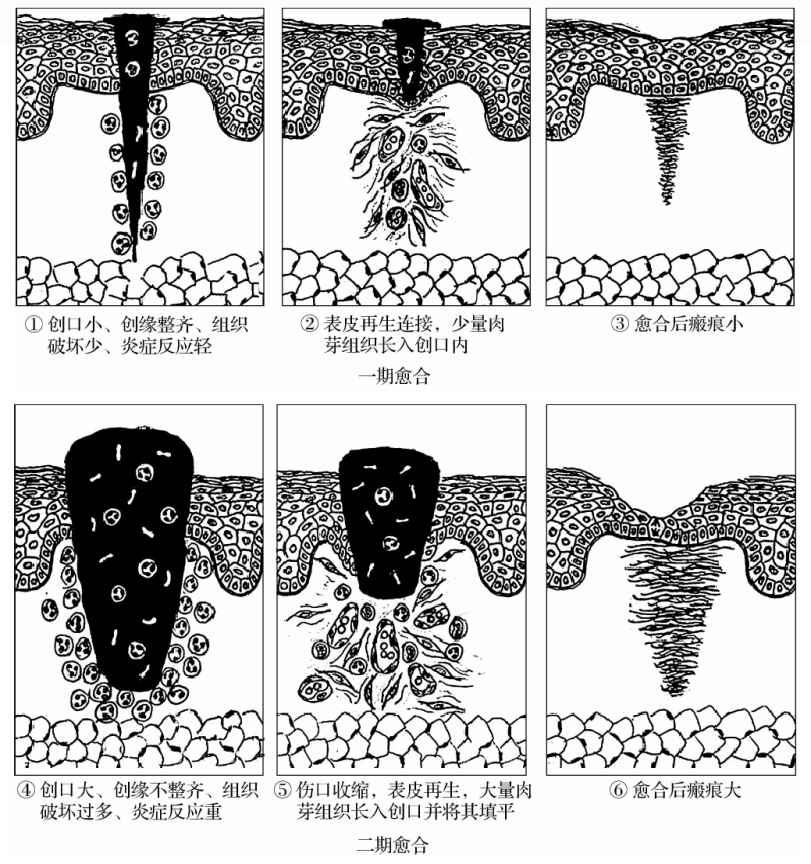
\includegraphics[width=0.5\textwidth]{./images/Image00030.jpg}
 \caption{人的胸腺}
 \label{fig2-5}
  \end{figure} 

人的胸腺(thymus)随年龄不同而有明显差别(图\ref{fig2-5})。新生期胸腺重量约15~20g;以后逐渐增大,青春期可达30~40g,其后随年龄增长而逐渐萎缩退化;老年期胸腺明显缩小,大部分被脂肪组织所取代。胸腺是T细胞分化、成熟的场所,其功能状态直接决定机体细胞免疫功能,并间接影响体液免疫功能。

(一)胸腺的解剖结构

胸腺的结构如图\ref{fig2-6}所示。一结缔组织被膜覆盖胸腺表面,并深入胸腺实质将其分隔成许多小叶。小叶的外层为皮质(cortex),内层为髓质(medulla),皮髓质交界处含大量血管,皮质内85\%~90\%的细胞为未成熟T细胞(即胸腺细胞),也存在少量上皮细胞、巨噬细胞(macrophage,Mφ)和树突状细胞(dendritic
cell,DC)等。胸腺浅皮质内发育早期的胸腺上皮细胞也称抚育细胞(nurse
cell),其在胸腺细胞分化中发挥重要作用。髓质内含大量上皮细胞和疏散分布的胸腺细胞、Mφ和DC。

\begin{figure}[!htbp]
 \centering
 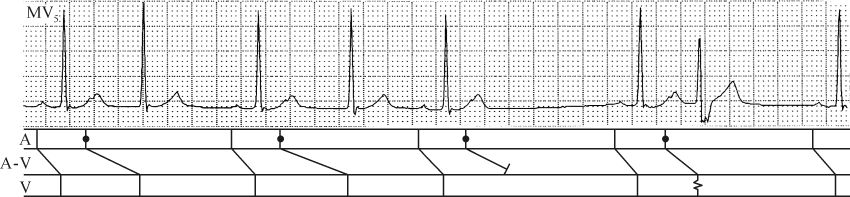
\includegraphics[width=0.7\textwidth]{./images/Image00031.jpg}
 \caption{胸腺结构示意图}
 \label{fig2-6}
  \end{figure} 

(二)胸腺的细胞组成:主要由胸腺基质细胞和胸腺细胞组成

1.胸腺基质细胞(thymic stromal cell,TSC):TSC以胸腺上皮细胞(thymus
epithelial
cell,TEC)为主,还包括巨噬细胞、DC及成纤维细胞等。TSC互相连接成网,并表达多种表面分子和分泌多种胸腺激素,从而构成重要的胸腺内环境。其中,抚育细胞与胸腺细胞通过各自表达的黏附分子密切接触,为胸腺细胞的发育提供必需的信号。

2.胸腺细胞:骨髓产生的前T细胞经血循环进入胸腺,即成为胸腺细胞。不同分化阶段的胸腺细胞其形态学、表面标志等各异,并可按其CD4、CD8表达情况分为4个亚群,即:CD4\textsuperscript{-}
CD8\textsuperscript{-} 、CD4\textsuperscript{+} CD8\textsuperscript{+}
、CD4\textsuperscript{+} CD8\textsuperscript{-} 、CD4\textsuperscript{-}
CD8\textsuperscript{+} 。

(三)胸腺微环境

胸腺微环境由TSC、细胞外基质及局部活性物质组成,其在胸腺细胞分化过程的不同环节均发挥重要作用。胸腺上皮细胞是胸腺微环境的最重要组分,其参与胸腺细胞分化的机制为:

1.分泌胸腺激素和细胞因子:主要的胸腺激素有胸腺素(thymosin)、胸腺刺激素(thymulin)、胸腺体液因子(thymic
humoral factor)、胸腺生成素(thymopoietin,TP)、血清胸腺因子(serum
thymic
factor)等。它们分别具有促进胸腺细胞增殖和分化、发育等功能。胸腺基质细胞还可产生多种细胞因子,它们通过与胸腺细胞表面相应受体结合,调节胸腺细胞发育和细胞间相互作用。上述胸腺激素和细胞因子是诱导胸腺细胞分化为成熟T细胞的必要条件。

2.与胸腺细胞相互接触:此乃通过上皮细胞与胸腺细胞间表面黏附分子及其配体、细胞因子及其受体、抗原肽-MHC分子复合物与TCR等相互作用而实现。

细胞外基质(extracellular
matrix)也是胸腺微环境的重要组成部分,它们可促进上皮细胞与胸腺细胞接触,并参与胸腺细胞在胸腺内移行成熟。

(四)胸腺的功能

1.T细胞分化、成熟的场所:胸腺是T细胞发育的主要场所。在胸腺产生的某些细胞因子作用下,来源于骨髓的前T细胞被吸引至胸腺内成为胸腺细胞。胸腺细胞循被膜下转移到皮质再向髓质移行,并经历十分复杂的选择性发育。在此过程中,约95\%的胸腺细胞发生以凋亡(apoptosis)为主的死亡而被淘汰,仅不足5\%的细胞分化为成熟T细胞。其特征为:表达成熟抗原受体(TCR)的CD4或CD8单阳性细胞;获得MHC限制性的抗原识别能力;获得自身耐受性。发育成熟的T细胞进入血循环,最终定居于外周免疫器官。

近期研究证实,胸腺并非T细胞分化发育的唯一场所。例如T细胞可在胸腺外组织(如肠道黏膜上皮、皮肤组织及泌尿生殖道黏膜组织等)中发育成熟。另外,肝脏也可能是某些T细胞分化发育的场所。

2.免疫调节功能:胸腺基质细胞可产生多种肽类激素,它们不仅促进胸腺细胞的分化成熟,也参与调节外周成熟T细胞。

3.屏障作用:皮质内毛细血管及其周围结构具有屏障作用,阻止血液中大分子物质进入,此为血-胸腺屏障(blood-thymus
barrier)。


\subsection{腔上囊}

腔上囊又称法氏囊(bursa of
fabricius),是鸟类动物特有的淋巴器官,位于胃肠道末端泄殖腔的后上方(图\ref{fig2-7})。与胸腺不同,腔上囊训化B细胞成熟,主导机体的体液免疫功能。将孵出的雏鸡去掉腔上囊,会使血中γ球蛋白缺乏,且没有浆细胞,注射疫苗亦不能产生抗体。人类和哺乳动物没有法氏囊,其功能由相似的组织器官代替,称为法氏囊同功器官;曾一度认为同功器官是阑尾、扁桃体和肠集结淋巴结,现在已证明是骨髓。

\begin{figure}[!htbp]
 \centering
 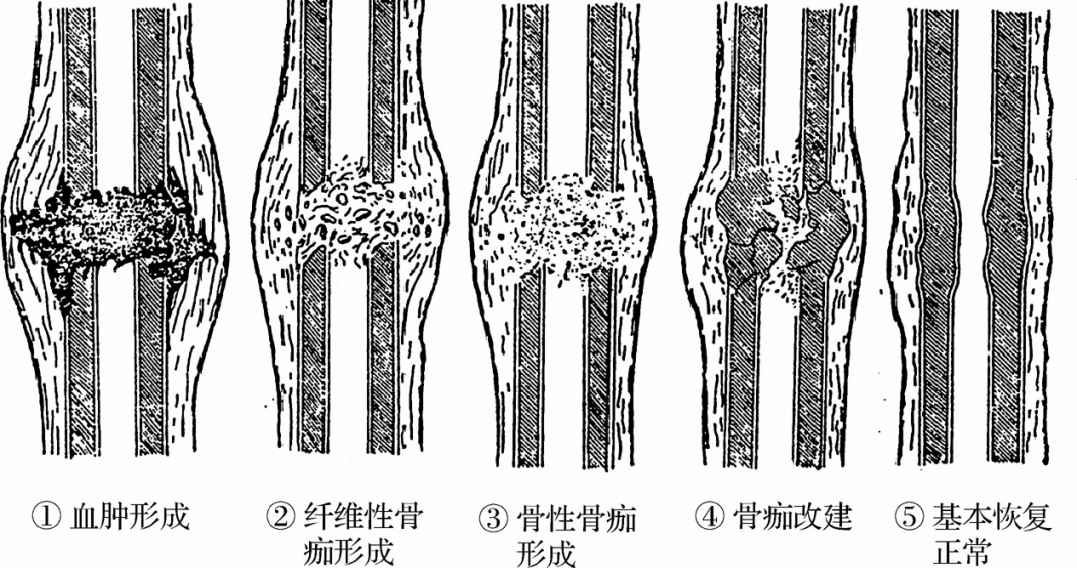
\includegraphics[width=.5\textwidth]{./images/Image00032.jpg}
 \caption{鸡的胸腺和法氏囊}
 \label{fig2-7}
  \end{figure} 

\section{外周免疫器官}

外周免疫器官(peripheral immune
organ)包括脾、淋巴结、淋巴样小结、扁桃体、阑尾等,这些器官内富含能捕捉和处理抗原的巨噬细胞和树突状细胞,以及能介导免疫反应的T细胞和B细胞。


\subsection{淋巴结}

淋巴结(lymph node)广泛分布于全身非黏膜部位的淋巴通道上。

(一)淋巴结的结构

淋巴结的结构如图\ref{fig2-8}所示,淋巴结表面覆盖有结缔组织被膜,后者深入实质形成小梁。淋巴结分为皮质和髓质两部分,彼此通过淋巴窦相通。被膜下为皮质,包括浅皮质区、副皮质区和皮质淋巴窦。

浅皮质区又称为非胸腺依赖区(thymus-independent
area),是B细胞定居的场所,该区内有淋巴滤泡(或称淋巴小结)。未受抗原刺激的淋巴小结无生发中心,称为初级滤泡(primary
follicle),主要含静止的成熟B细胞;受抗原刺激的淋巴小结内出现生发中心(germinal
center),称为次级滤泡(secondary
follicle),内含大量增殖分化的B淋巴母细胞,此细胞向内转移至淋巴结中心部髓质,即转化为可产生抗体的浆细胞。

副皮质区又称胸腺依赖区(thymus-dependent
area),位于浅皮质区和髓质之间,为深皮质区,是T细胞(主要是CD\textsuperscript{+}
\textsubscript{4}
T细胞)定居的场所。该区有许多由内皮细胞组成的毛细血管后微静脉,也称高内皮细胞小静脉(high
endothelial venule,HEV),在淋巴细胞再循环中起重要作用。

髓质由髓索和髓窦组成。髓索内含有
B细胞、T细胞、浆细胞、肥大细胞及Mφ。髓窦内Mφ较多,有较强滤过作用。

\begin{figure}[!htbp]
 \centering
 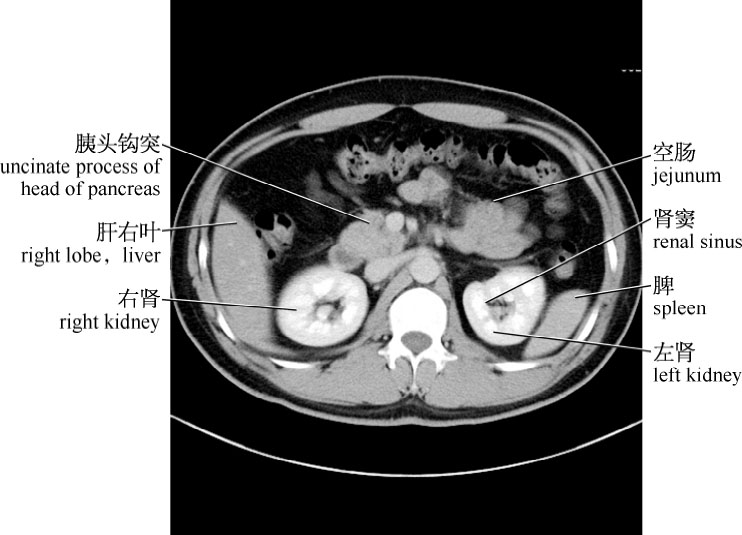
\includegraphics[width=.6\textwidth]{./images/Image00033.jpg}
 \caption{淋巴结的结构}
 \label{fig2-8}
  \end{figure} 

(二)淋巴结的功能

1.T 细胞及
B细胞定居的场所:分别在胸腺和骨髓中分化成熟的T、B细胞,均可定居于淋巴结。其中,T细胞占淋巴结内淋巴细胞总数的75\%,B细胞占25\%。

2.免疫应答发生的场所:抗原递呈细胞携带所摄取的抗原进入淋巴结,将已被加工、处理的抗原递呈给淋巴结内的T细胞和B细胞,使之活化、增殖、分化,故淋巴结是发生细胞免疫和体液免疫应答的主要场所。

3.参与淋巴细胞再循环:淋巴结深皮质区的HEV在淋巴细胞再循环中发挥重要作用,血循环中的淋巴细胞穿越HEV壁进入淋巴结实质,然后通过输出淋巴管进入胸导管或右淋巴管,再回到血液循环。

4.过滤作用:组织中的病原微生物及毒素等进入淋巴液,其缓慢流经淋巴结时,可被Mφ吞噬或通过其他机制被清除。因此,淋巴结具有重要的滤过作用。


\subsection{脾脏}

(一)脾脏的结构

脾脏的结构如图\ref{fig2-9}所示,脾脏(spleen)是人体最大的淋巴器官,可分为白髓、红髓和边缘区三部分。白髓由密集的淋巴组织构成,包括动脉周围淋巴鞘和淋巴小结。动脉周围淋巴鞘为T细胞居住区;鞘内的淋巴小结为B细胞居住区,未受抗原刺激为初级滤泡,受抗原刺激后出现生发中心,为次级滤泡。红髓分布于白髓周围,包括髓索和髓窦:前者主要为B细胞居留区,也含Mφ和DC;髓窦内为循环的血液。白髓与红髓交界处为边缘区(marginal
zone),是血液及淋巴细胞进出的重要通道。

\begin{figure}[!htbp]
 \centering
 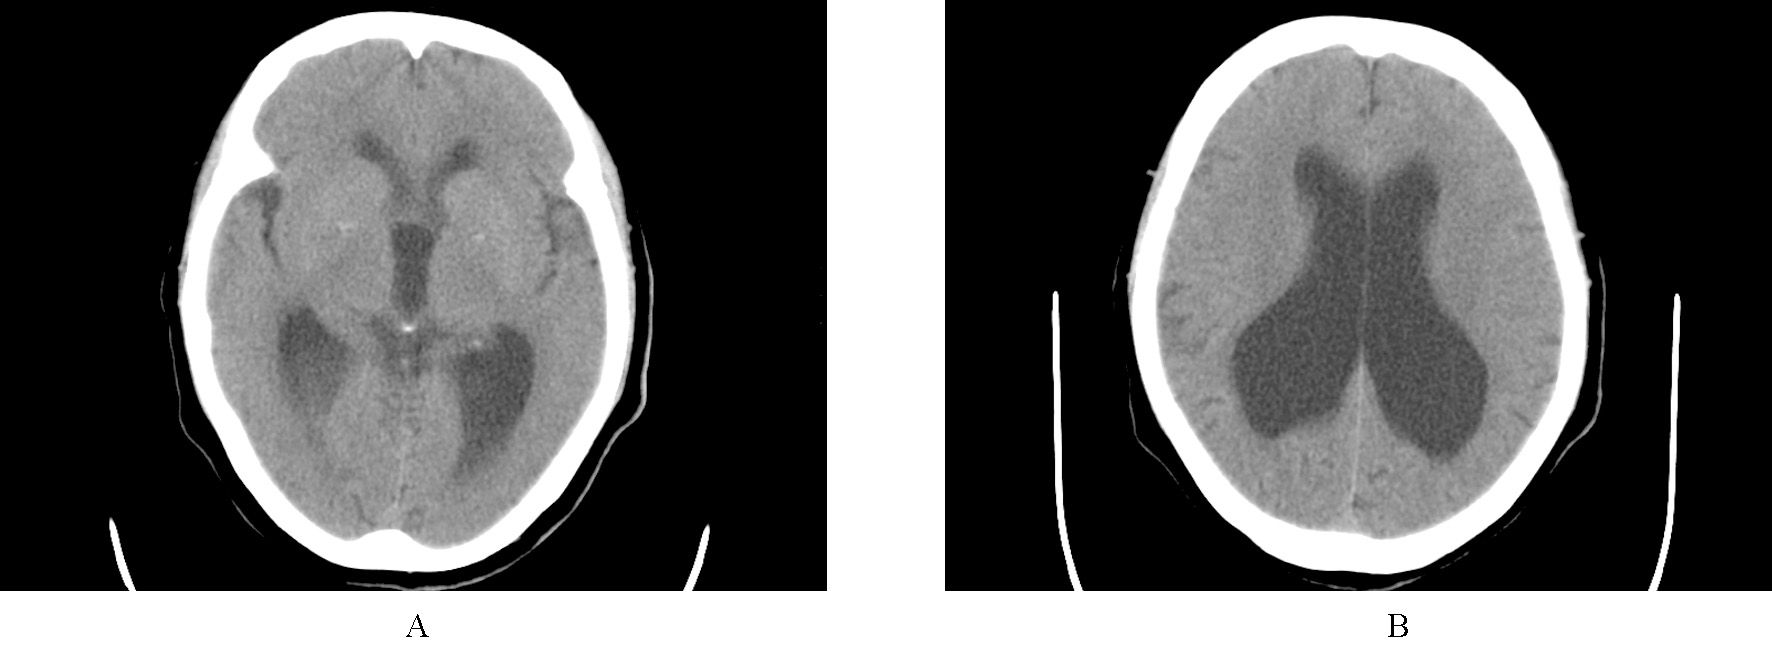
\includegraphics[width=.5\textwidth]{./images/Image00034.jpg}
 \caption{脾脏的结构}
 \label{fig2-9}
  \end{figure} 

(二)脾脏的功能

脾脏是重要的外周免疫器官,脾切除的个体其免疫防御功能可发生障碍。

1.免疫细胞定居的场所:成熟的淋巴细胞可定居于脾脏。B细胞约占脾脏中淋巴细胞总数的60\%,T细胞约占40\%。

2.免疫应答的场所:脾脏也是淋巴细胞接受抗原刺激并发生免疫应答的重要部位。同为外周免疫器官,脾脏与淋巴结的差别在于:脾脏是对血源性抗原产生应答的主要场所。

3.合成生物活性物质:脾脏可合成并分泌如补体、干扰素等生物活性物质。

4.滤过作用:脾脏可清除血液中的病原体、衰老死亡的自身血细胞、某些蜕变细胞及免疫复合物等,从而使血液得到净化。

此外,脾脏也是机体贮存红细胞的血库。


\subsection{黏膜相关淋巴组织}

黏膜相关淋巴组织(mucosal-associated lymphoid
tissue,MALT)亦称黏膜免疫系统(mucosal lymphoid
system,MIS),主要指呼吸道、肠道及泌尿生殖道黏膜固有层和上皮细胞下散在的无被膜淋巴组织以及某些带有生发中心的器官化淋巴组织,如扁桃体、小肠的派氏集合淋巴结(Peyer
patche)、阑尾等。

黏膜系统在机体免疫防疫机制中的重要作用表现为:①人体黏膜的表面积约400平方米,乃阻止病原微生物等入侵机体的主要物理屏障;②机体近一半的淋巴组织存在于黏膜系统,故MALT被视为执行局部特异性免疫功能的主要部位。

(一)MALT的组成

1.鼻相关淋巴组织(nasal-associated lymphoid
tissue,NALT):包括咽扁桃体、腭扁桃体、舌扁桃体及鼻后部其他淋巴组织,其主要作用是抵御经空气传播的微生物感染。

2.肠相关淋巴组织(gut-associated lymphoid
tissue,GALT):GALT包括集合淋巴结、淋巴滤泡和固有层淋巴组织等,其主要作用是抵御侵入肠道的病原微生物感染(图\ref{fig2-10})。肠道黏膜上皮间还散布一种扁平上皮细胞,即M细胞(membranous
cell or microfold
cell,膜性细胞或微皱褶细胞),又称特化的抗原转运细胞(specialized
antigen transporting
cell),是散布于肠道黏膜上皮细胞间的一种特化的抗原运转细胞。它不表达MHCⅡ类分子,胞质内溶毛体很少,在肠黏膜表面有短小不规则毛刷样微绒毛。M细胞的基底部凹陷成小袋,其中容纳T细胞、B细胞、巨噬细胞、DC等。M细胞具有高度的非特异性脂酶活性,病原菌等外来抗原性物质可通过对M细胞表面的毛刷状微绒毛的吸附,或经M细胞表面蛋白酶作用后被摄取,并将未降解的抗原转运给小袋中的巨噬细胞,由后者携带抗原至集合淋巴结,引发黏膜免疫应答,肠道淋巴系统免疫应答如图\ref{fig2-11}所示。

\begin{figure}[!htbp]
 \centering
 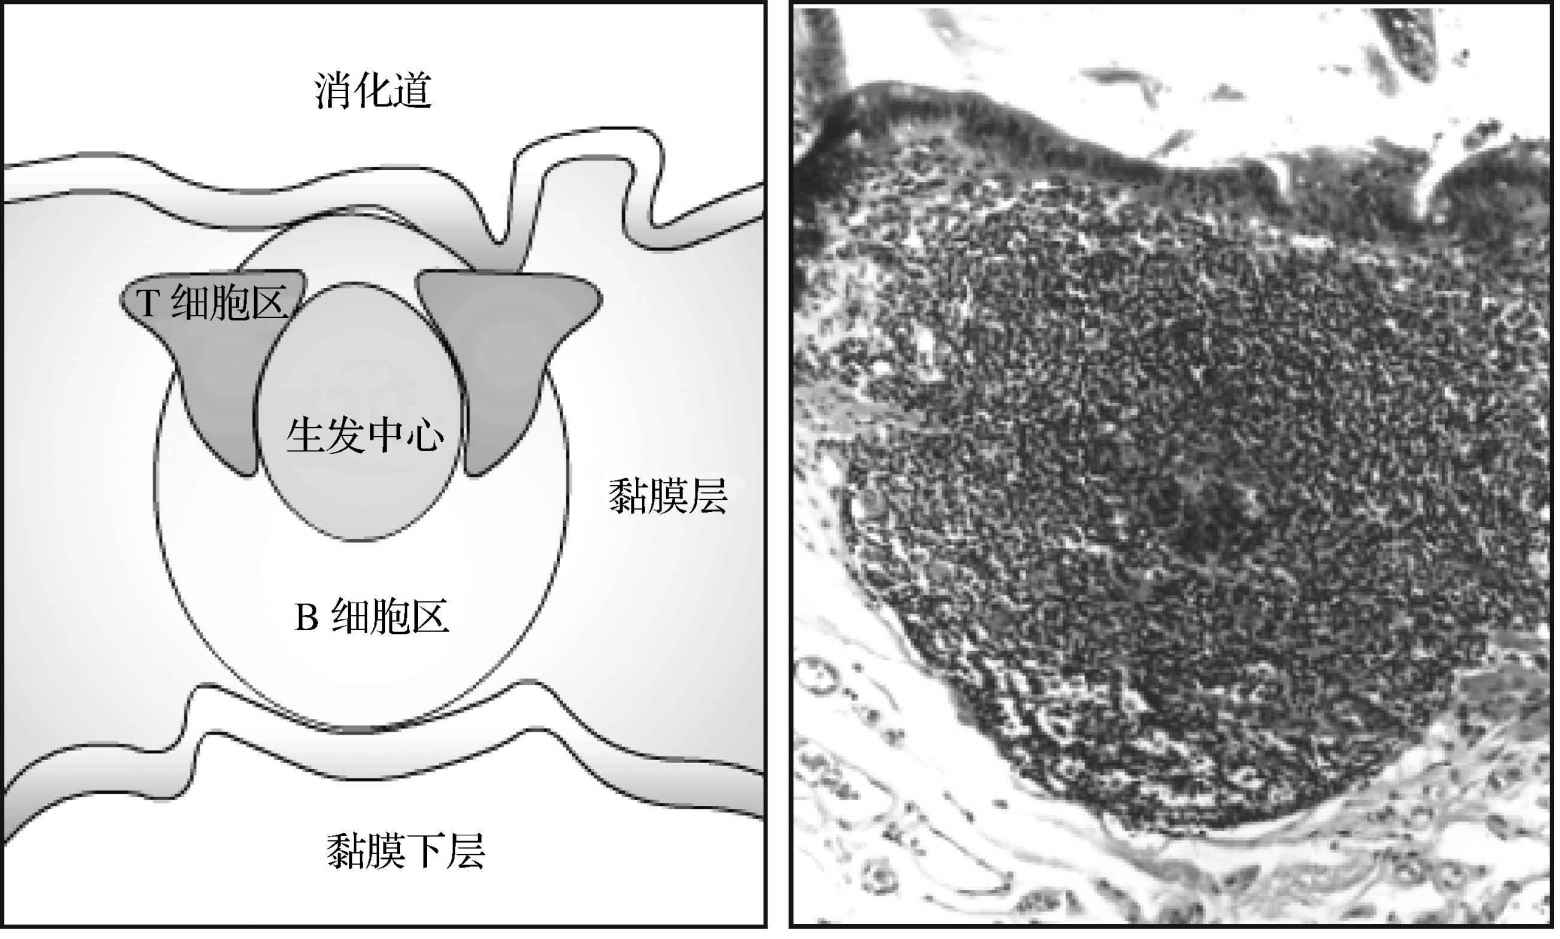
\includegraphics[width=.5\textwidth]{./images/Image00035.jpg}
 \caption{消化道集合淋巴滤泡}
 \label{fig2-10}
  \end{figure} 

\begin{figure}[!htbp]
 \centering
 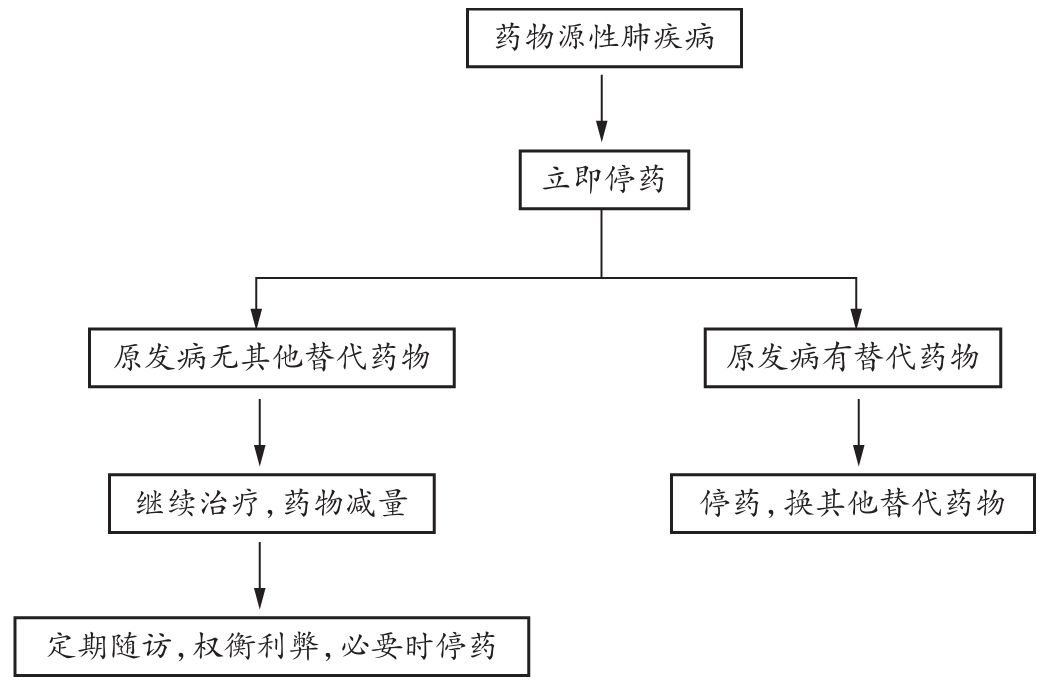
\includegraphics[width=.6\textwidth]{./images/Image00036.jpg}
 \caption{肠道M细胞的转运功能及M细胞包围住大肠杆菌}
 \label{fig2-11}
  \end{figure} 

黏膜免疫系统在保护黏膜表面不受病原体侵害、促进与共生微生物群落共生中都起主要作用。要激发黏膜免疫反应,黏膜表面上的抗原必须首先穿过不可透过的上皮障碍,进入“派伊尔小结”这样的淋巴结构。这一功能(被称为“转胞吞作用”)被认为主要由M细胞调控,它们是“派伊尔小结”中专门的上皮细胞。对由M-细胞调控的抗原“转胞吞作用”的机制所做的一项研究表明,在小肠M细胞顶面表达的糖蛋白-2是表达FimH抗原的细菌的转胞吞受体。由于M-细胞被认为是各种口服免疫药物的一个很有希望的目标,所以这项工作表明,依赖于糖蛋白-2的“转胞吞作用”是一个可能的免疫目标。

3.支气管相关淋巴组织(bronchial-associated
tissue,BALT):主要分布于各肺叶的支气管上皮下,其结构与派氏集合淋巴结相似,滤泡中淋巴细胞受抗原刺激常增生成生发中心,其中主要是B细胞。

(二)MALT的功能及其特点

1.参与局部免疫应答:分布在不同部位的MALT均是参与局部特异性免疫应答的主要场所,从而在消化道、呼吸道和泌尿生殖道的局部免疫防御中发挥关键作用。

2.分泌型IgA(secretory
IgA,SIgA):以消化道黏膜为例,口服抗原被吸收进入集合淋巴结后,可引发B细胞应答,使之转化为产生抗体的浆细胞,其中可分泌SIgA的浆细胞主要定居于集合淋巴结或迁移至固有层。SIgA在抵御病原体侵袭消化道、呼吸道和泌尿生殖道中发挥重要作用。

3.参与口服抗原介导的免疫耐受:口服蛋白抗原刺激黏膜免疫系统后,常可导致免疫耐受,其机制尚未阐明。口服抗原诱导耐受的生物学意义在于:①可阻止机体对肠腔内共栖的正常菌群产生免疫应答,而这些菌群的存在乃正常消化和吸收功能所必需;②通过口服抗原诱导机体对该抗原形成特异性无反应性,可能为治疗自身免疫病提供新途径。

\begin{center}
\textbf{\Large 附:淋巴细胞再循环}
\end{center}

各种免疫器官中的淋巴细胞并不是定居不动的群体,而是通过血液和淋巴液的循环进行有规律的迁移,这种规律性的迁移为淋巴细胞再循环(lymphocyterecirculation)。通过再循环,可以增加淋巴细胞与抗原接触的机会,更有效地激发免疫应答,并不断更新和补充循环池的淋巴细胞。

1.再循环的细胞淋巴干细胞从骨髓迁移至胸腺和腔上囊或其功能器官,分化成熟后进入血液循环的定向移动过程不属于再循环范围。再循环是成熟淋巴细胞通过循环途径实现淋巴细胞不断重新分布的过程。再循环中的细胞多是静止期细胞和记忆细胞,其中80%以上是T细胞。这些细胞最初来源于胸腺和骨髓;成年以后,主要靠外周免疫器官进行补充。受抗原刺激而活化的淋巴细胞很快定居于外周免疫器官,不再参加再循环。

2.再循环的途径血液中的淋巴细胞在流经外周免疫器官(以淋巴结为例)时,在副皮质区与皮质区的连接处穿过高内皮毛细血管后静脉(HEV)进入淋巴结;T细胞定位于副皮质,B细胞主要定位于皮质区;以后均通过淋巴结髓窦迁移至输出淋巴管,进入高一级淋巴结;经过类似的路径,所有外周免疫器官输出的细胞最后都汇集于淋巴导管;身体下部和左上部的汇集到胸导管,从左锁骨下静脉角返回血循环;右侧上部的汇集到右淋巴管,从右锁骨下静脉返回血循环。再循环一周约需24~48小时。

3.细胞定居选择淋巴细胞从血循环进入淋巴组织具有高度的选择性,这是因为淋巴细胞上具有特殊的受体分子,称为归巢受体(homingreceptor)。现已发现的归巢受体包括CD44、LFA-1、VLA-4和MEL-14/LAM-1等;其中MEL-14/LAM-1是定居淋巴结的受体,识别淋巴结内的高内皮细胞;VLA-4的α亚单位是定居MALT的受体,识别黏膜表面的配体。

淋巴细胞再循环的意义:带有不同特异性抗原受体的各种淋巴细胞不断在体内各处巡游,增加了与抗原以及抗原递呈细胞接触的机会;许多免疫记忆细胞也参与淋巴细胞再循环,一旦接触到相应抗原,可立即进入淋巴组织发生增殖反应,产生免疫应答。淋巴细胞再循环如图\ref{fig2-12}所示。

\begin{figure}[!htbp]
 \centering
 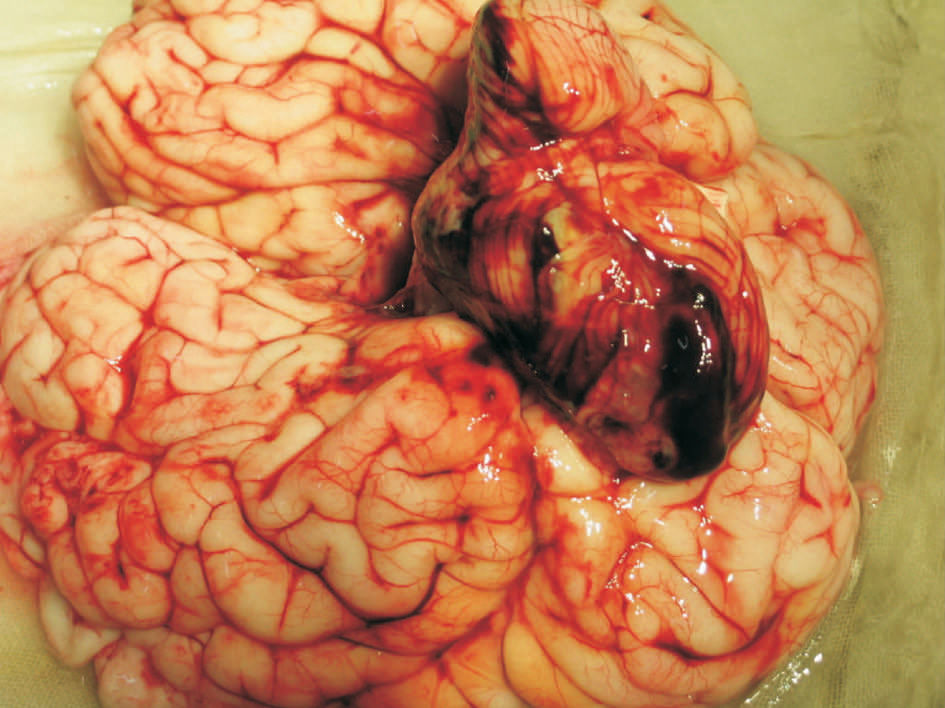
\includegraphics[width=.6\textwidth]{./images/Image00037.jpg}
 \caption{淋巴细胞再循环示意图}
 \label{fig2-12}
  \end{figure} 

\section{免疫细胞}

免疫细胞乃泛指所有参与免疫应答或与免疫应答有关的细胞及其前体,包括造血干细胞、淋巴细胞、专职抗原递呈细胞(树突状细胞、单核-巨噬细胞)及其他抗原递呈细胞、粒细胞、肥大细胞和红细胞等,如图\ref{fig2-13}所示。

\begin{figure}[!htbp]
 \centering
 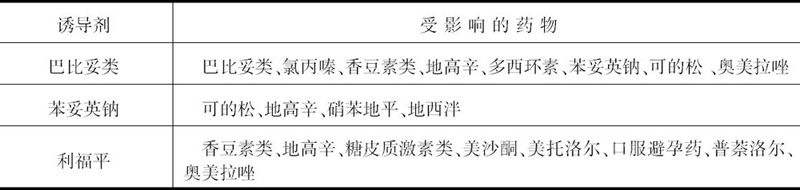
\includegraphics[width=.6\textwidth]{./images/Image00038.jpg}
 \caption{各种免疫细胞}
 \label{fig2-13}
  \end{figure} 


\subsection{造血干细胞}

造血干细胞(hemopoietic stem
cell,HSC)又称多能干细胞,是存在于造血组织中的一群原始造血细胞。也可以说,它是一切血细胞(其中大多数是免疫细胞)的原始细胞。由造血干细胞定向分化、增殖为不同的血细胞系,并进一步生成血细胞。人类造血干细胞首先出现于胚龄第2~3周的卵黄囊,在胚胎早期(第2~3月)迁至肝、脾,第5个月又从肝、脾迁至骨髓。在胚胎末期一直到出生后,骨髓成为造血干细胞的主要来源,具有多潜能性,即具有自身复制和分化两种功能。


\subsection{淋巴细胞}

淋巴细胞(lymphocyte)是构成免疫系统的主要细胞类别,占外周血白细胞总数的20%~45%,成年人体内约有10\textsuperscript{12}
个淋巴细胞。淋巴细胞可分为许多表型与功能均不同的群体,如T细胞、B细胞、NK细胞等;T细胞和B细胞还可进一步分为若干亚群。这些淋巴细胞及其亚群在免疫应答过程中相互协作、相互制约,共同完成对抗原物质的识别、应答和清除,从而维持机体内环境的稳定。

其特点是:未活化淋巴细胞在抗原的刺激下转变为淋巴母细胞,再进一步转变为效应T细胞与记忆细胞。可分群为:
\begin{itemize}
\item T细胞:细胞膜上表达CD3分子和TCR
\item B细胞:细胞膜上表达BCR
\item NK细胞:细胞膜上表达CD56和CD16
\end{itemize}

(一)T淋巴细胞

T淋巴细胞(T
lymphocyte)简称T细胞,其介导细胞免疫应答,并在机体针对TD抗原的体液免疫应答中发挥重要的辅助作用。骨髓中的淋巴样前体细胞(lymphoid
precursor)进入胸腺,经历一系列有序的分化过程,才能发育为成熟T细胞。T细胞乃高度异质性的细胞群,依据其表面标志及功能特征,可分为若干亚群。在免疫应答过程中,各亚群T细胞相互协作,共同发挥重要的免疫学功能。

1.T细胞的表面标志

T细胞表面标志即其膜分子(如图\ref{fig2-14}所示),是T细胞识别抗原、与其他免疫细胞相互作用、接受信号刺激并产生应答的物质基础,亦是鉴别和分离T细胞的重要依据。在诸多表面标志中,TCR、CD3分子是外周血成熟T细胞各亚群的共有标志。

(1)T细胞表面受体(surface antigen):T细胞抗原受体(T cell antigen
receptor,TCR)、细胞因子受体(cytokine receptor,CKR)、丝裂原受体。

(2)T细胞表面抗原(surface antigen):MHC抗原、分化抗原(CD分子)等。

\begin{figure}[!htbp]
 \centering
 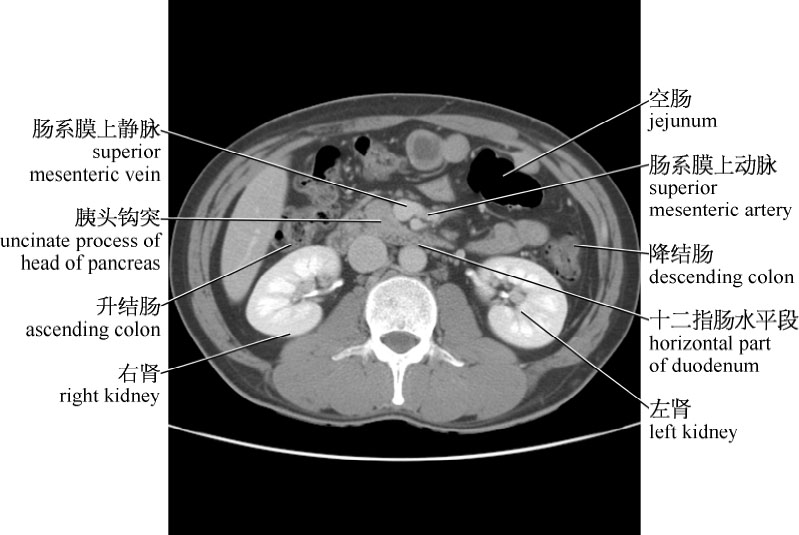
\includegraphics{./images/Image00039.jpg}
 \caption{T细胞表面标志}
 \label{fig2-14}
  \end{figure} 

2.T细胞亚群及其功能

人类的T细胞不是均一的群体,根据表面标志和功能可为五个亚群:

CD4\textsuperscript{+}
T(初始T细胞,Th1细胞,Th2细胞):占T细胞的65\%左右,它的重要标志是表面有CD4抗原。Th细胞能识别抗原,分泌多种淋巴因子,它既能辅助B细胞产生体液免疫应答,又能辅助T细胞产生细胞免疫应答,是扩大免疫应答的主要成分,它还具有某些细胞免疫功能。

CD8\textsuperscript{+}
T(杀伤性T细胞,抑制性T细胞):杀伤性T细胞占T细胞的20%~30%,表面也有CD8抗原。杀伤性T细胞能识别结合在MHC-Ⅰ类抗原上的异抗原,在异抗原的刺激下可增殖形成大量效应性杀伤性T细胞,能特异性地杀伤靶细胞,是细胞免疫应答的主要成分。抑制性T细胞占T细胞的10%左右,表面有CD8抗原。抑制性T细胞常在免疫应答的后期增多,它分泌的抑制因子可减弱或抑制免疫应答。

(1)初始T细胞(naive T
cell):指未完全分化的Th细胞,是Th1、Th2细胞的前体,分泌低水平的IL-4和IFN-γ。

功能:调节体液免疫应答和细胞免疫应答,分化产生Th1、Th2细胞,T细胞的分化如图\ref{fig2-15}所示。

\begin{figure}[!htbp]
 \centering
 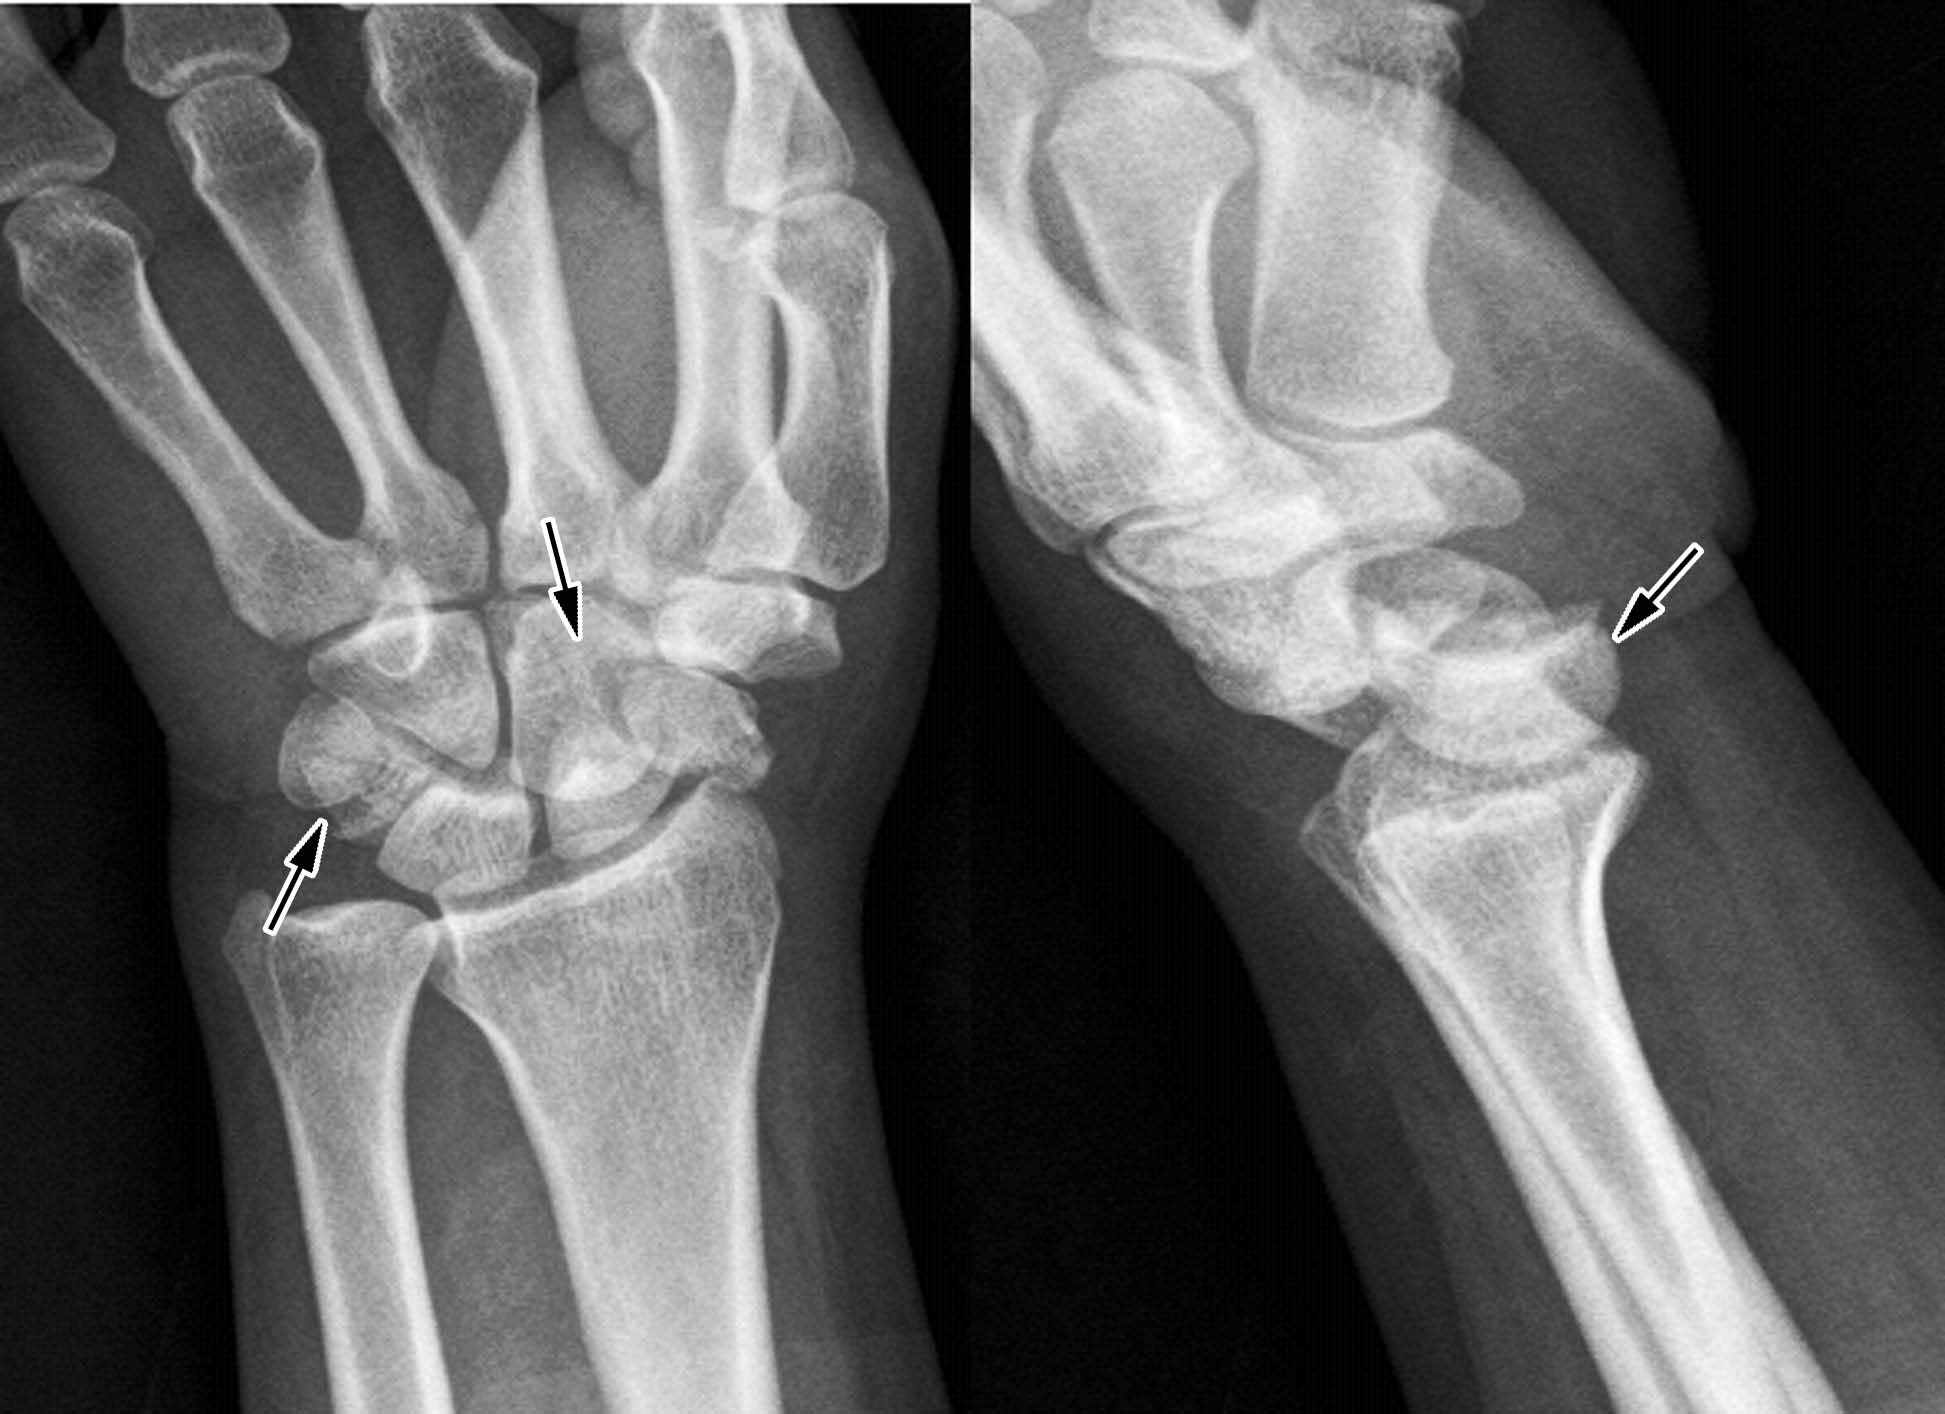
\includegraphics{./images/Image00040.jpg}
 \caption{T细胞的分化}
 \label{fig2-15}
  \end{figure} 

按分泌的细胞因子不同可将Th细胞分为两个不同的亚群:分泌IFN-γ、IL-2的称为TH1细胞,分泌IL-4、IL-5的称为Th2细胞。

(2)Th1细胞:初始T细胞在IL-12作用下转变为Th1细胞。

Th1细胞功能:释放IL-2、IFN-γ和TNF,引起炎症反应或迟发型超敏反应,称为炎症性T细胞。参与细胞免疫应答及迟发型超敏反应。在抗胞内病原微生物等感染中起重要作用。Th1细胞持续性强应答,可能与器官特异性自身免疫病、接触性皮炎、不明原因的慢性炎症性疾病、迟发型超敏反应性疾病、急性同种异体移植排斥反应等的发生有关。

(3)Th2细胞:初始T细胞在IL-4作用下转变为Th2细胞。

释放IL-4、5、6、10,诱导B细胞增殖分化、合成并分泌抗体,引起体液免疫应答或速发型超敏反应(图\ref{fig2-16})。

\begin{figure}[!htbp]
 \centering
 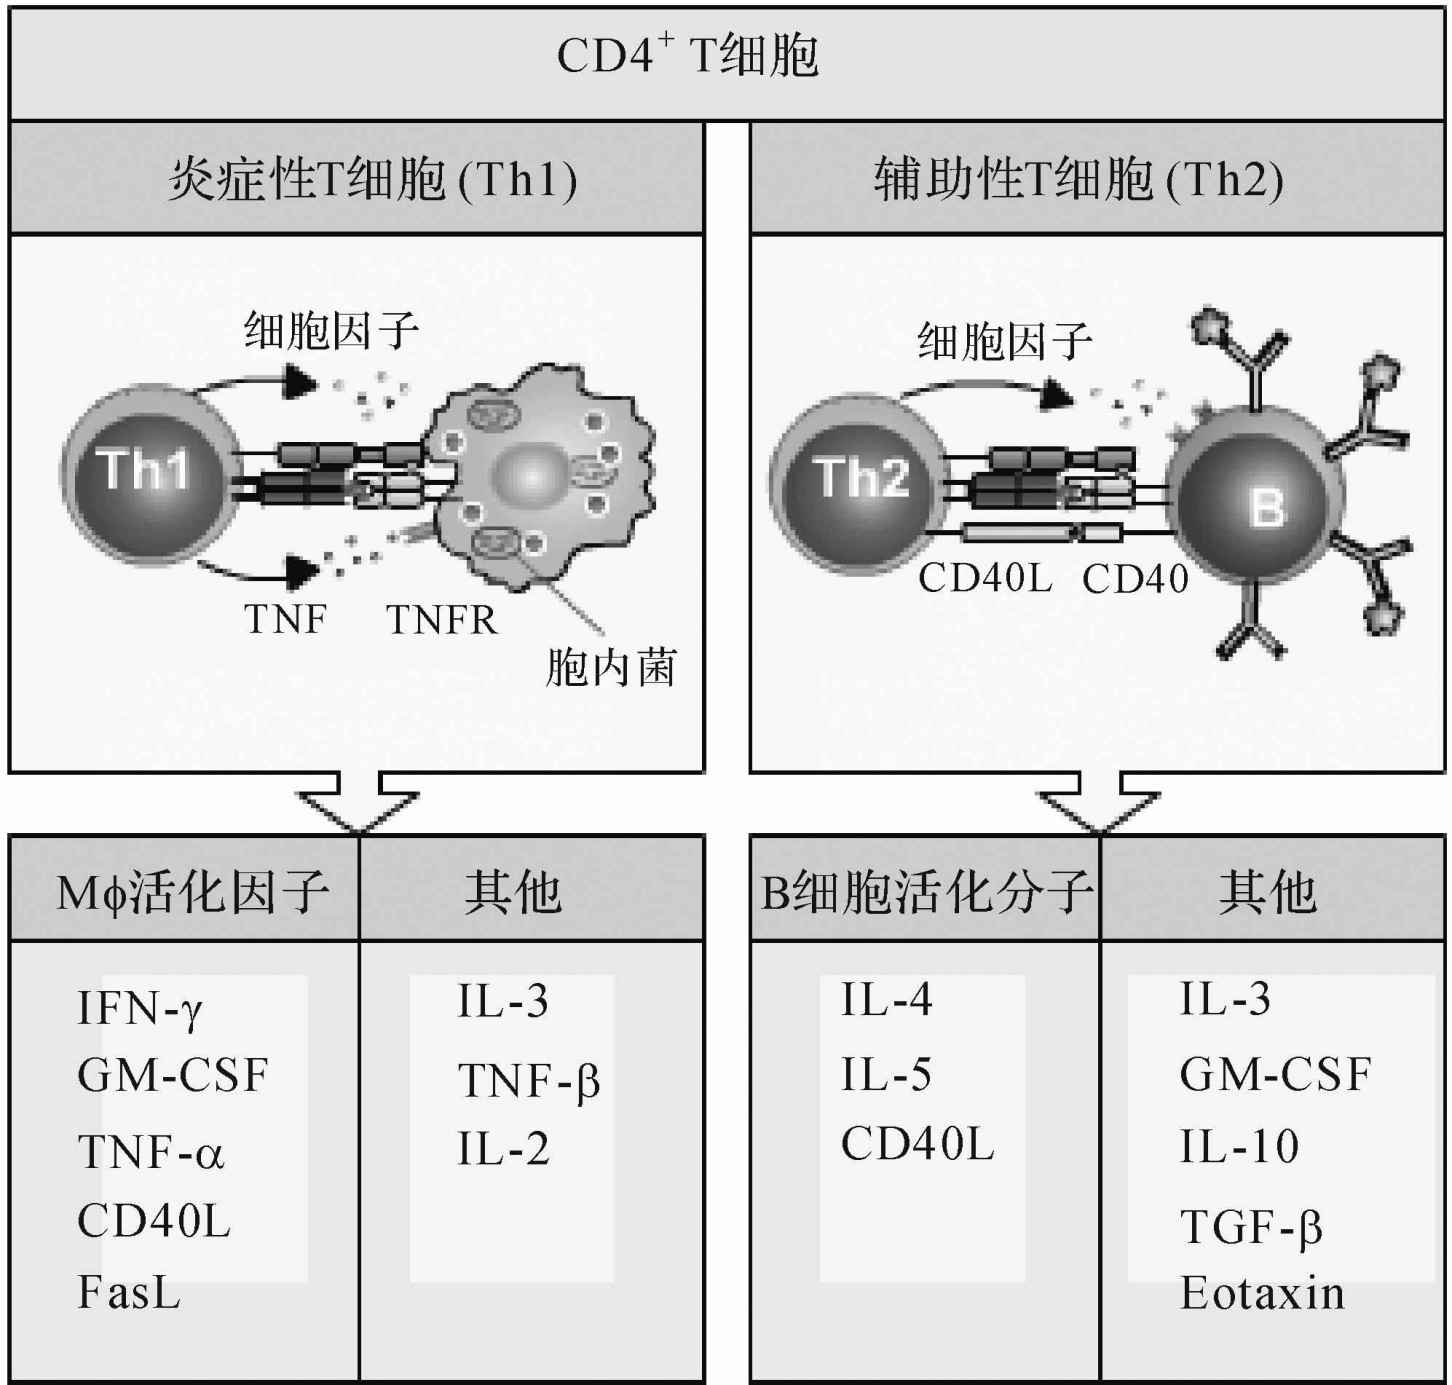
\includegraphics[width=.5\textwidth]{./images/Image00041.jpg}
 \caption{Th1、Th2淋巴细胞的功能}
 \label{fig2-16}
  \end{figure} 

(4)杀伤性T细胞(CTL):也叫细胞毒性T细胞,是效应T细胞,经抗原致敏后,CTL
的TCR特异性识别靶细胞(如病毒感染细胞、肿瘤细胞、同种异体移植物细胞等)表面的抗原肽/MHC-I类分子复合物。活化CTL
杀伤效应的主要机制为:①分泌穿孔素(perforin)、颗粒酶(granzyme)或淋巴毒素等直接杀伤靶细胞;②通过高表达FasL导致Fas阳性的靶细胞凋亡。CTL参与的免疫效应为抗病毒感染、抗肿瘤和介导同种异体移植排斥反应等(图\ref{fig2-17})。

\begin{figure}[!htbp]
 \centering
 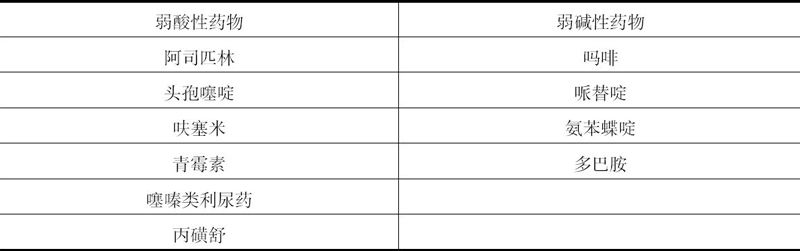
\includegraphics[width=.5\textwidth]{./images/Image00042.jpg}
 \caption{CTL的免疫效应}
 \label{fig2-17}
  \end{figure} 

(5)Ts细胞(suppressor T cell,Ts):具有抑制体液免疫和细胞免疫的功能。

(二)B淋巴细胞

B淋巴细胞(B
lymphocyte)是始祖B淋巴细胞在骨髓(人、动物)、法氏囊(禽)中发育、分化、成熟,产生抗体,也称骨髓或囊依赖性细胞,是体内唯一能产生抗体(Ig)的细胞,主要执行体液免疫,也具有抗原递呈功能。外周血中占淋巴细胞总数10\%~15\%,简称B细胞,是由哺乳动物骨髓或鸟类法氏囊中的淋巴样前体细胞分化成熟而来。

1.B细胞的表面标志

B细胞表面标志如图\ref{fig2-18}所示。

\begin{figure}[!htbp]
 \centering
 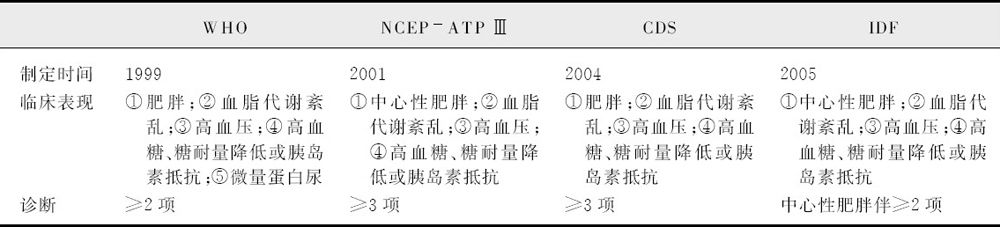
\includegraphics[width=.5\textwidth]{./images/Image00043.jpg}
 \caption{B细胞表面标志}
 \label{fig2-18}
  \end{figure} 

(1)B细胞抗原受体(B-cell antigen
receptor,BCR):BCR是嵌入细胞膜类脂分子中的膜表面免疫球蛋白(mIg),乃B细胞的特征性表面标志,也是B细胞特异性识别不同抗原表位的分子基础。

(2)细胞因子受体:B细胞表面表达IL-1R、IL-2R、IL-4R、IL-5R、IL-6R、IL-7R及IFN-γR等多种细胞因子受体。细胞因子通过与B细胞表面相应受体结合而参与或调节B细胞活化、增殖和分化。

(3)补体受体(CR):多数B细胞表面表达CR1和CR2(即CD35和CD21)。CR1主要见于成熟B细胞,其在B细胞活化后表达增高。CR1与相应配体结合可促进B细胞活化。CR2(CD21)是EB病毒受体,在体外应用EB病毒感染B细胞可使之转化为B淋巴母细胞系,从而达到永生化(immortalized)。

(4)Fc受体:多数B细胞表达IgG Fc受体Ⅱ(FcγRⅡ),可与免疫复合物中的IgG
Fc段结合,有利于B细胞捕获和结合抗原,并促进B细胞活化和抗体产生。

(5)丝裂原受体:某些丝裂原通过与B细胞表面相应受体结合,使其被激活并增殖分化为淋巴母细胞,可用于检测B细胞功能状态。美洲商陆(PWM)对T细胞和B细胞均有致有丝分裂作用;脂多糖(LPS)是常用的小鼠B细胞丝裂原。

2.细胞表面抗原

(1)MHC抗原:B细胞可表达MHC-Ⅰ类和MHC-Ⅱ类抗原。MHC-Ⅱ类抗原可与Th细胞表面CD4结合,增强B细胞与Th细胞间的黏附作用,并参与抗原递呈和淋巴细胞激活。

(2)CD抗原:B细胞分化发育的不同阶段,其CD抗原的表达各异,有CD19、CD20、CD21、CD40/CD40L、CD80(B7-1)/CD86(B7-2)。

3.B细胞亚群及功能

根据是否表达CD5分子,可将人B细胞分为B1(CD\textsuperscript{+}
\textsubscript{5} )和B2(CD\textsuperscript{-} \textsubscript{5}
)细胞。

(1)B1细胞亚群:B1细胞在个体发育过程中出现较早,是由胚胎期或出生后早期的前体细胞分化而来,其发生不依赖于骨髓细胞。B1细胞产生后,成为具有自我更新(self-renewal)能力的长寿细胞,主要分布于胸腔、腹腔和肠壁固有层中。B1细胞的抗原识别谱较窄,主要针对属于TI-2抗原的多糖类物质,尤其是某些菌体表面共有的多糖抗原(如肺炎球菌荚膜多糖等)。B1细胞的功能特点是:主要产生IgM类的低亲和力抗体;不发生抗体类别转换;无免疫记忆。

(2)B2细胞亚群:B2细胞即通常所称的B细胞,是参与体液免疫应答的主要细胞类别。它是由骨髓中多能造血干细胞分化而来,属形态较小、比较成熟的B细胞,在体内出现较晚,定位于外周淋巴器官。B2细胞的主要生物学功能为:参与体液免疫应答、抗原递呈、免疫调节。

(三)自然杀伤细胞

自然杀伤细胞(natural
killer,NK)是一类独立的淋巴细胞群,其不同于T细胞和B细胞,不表达特异性抗原识别受体(图\ref{fig2-19})。NK细胞胞浆内有许多嗜苯胺颗粒,故又称为大颗粒淋巴细胞(large
granular
lymphocyte)。NK细胞无须抗原预先致敏即可直接杀伤某些靶细胞,包括肿瘤细胞、病毒或细菌感染的细胞以及机体某些正常细胞(图\ref{fig2-20})。
\begin{figure}[!htbp]
    \centering
    \begin{minipage}[b]{0.45\textwidth} 
      \centering
        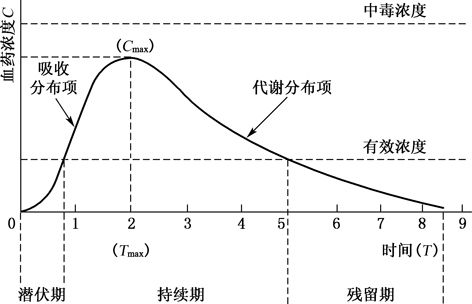
\includegraphics[height=0.12\textheight]{./images/Image00044.jpg}
        \captionsetup{justification=centering}
        \caption{自然杀伤细胞}
        \label{fig2-19}
    \end{minipage}
%	\end{figure} 
	%\FloatBarrier
%\begin{figure}[!htbp]
%    \centering
%\hspace{0.04\textwidth}%
\begin{minipage}[b]{0.45\textwidth} 
  \centering
    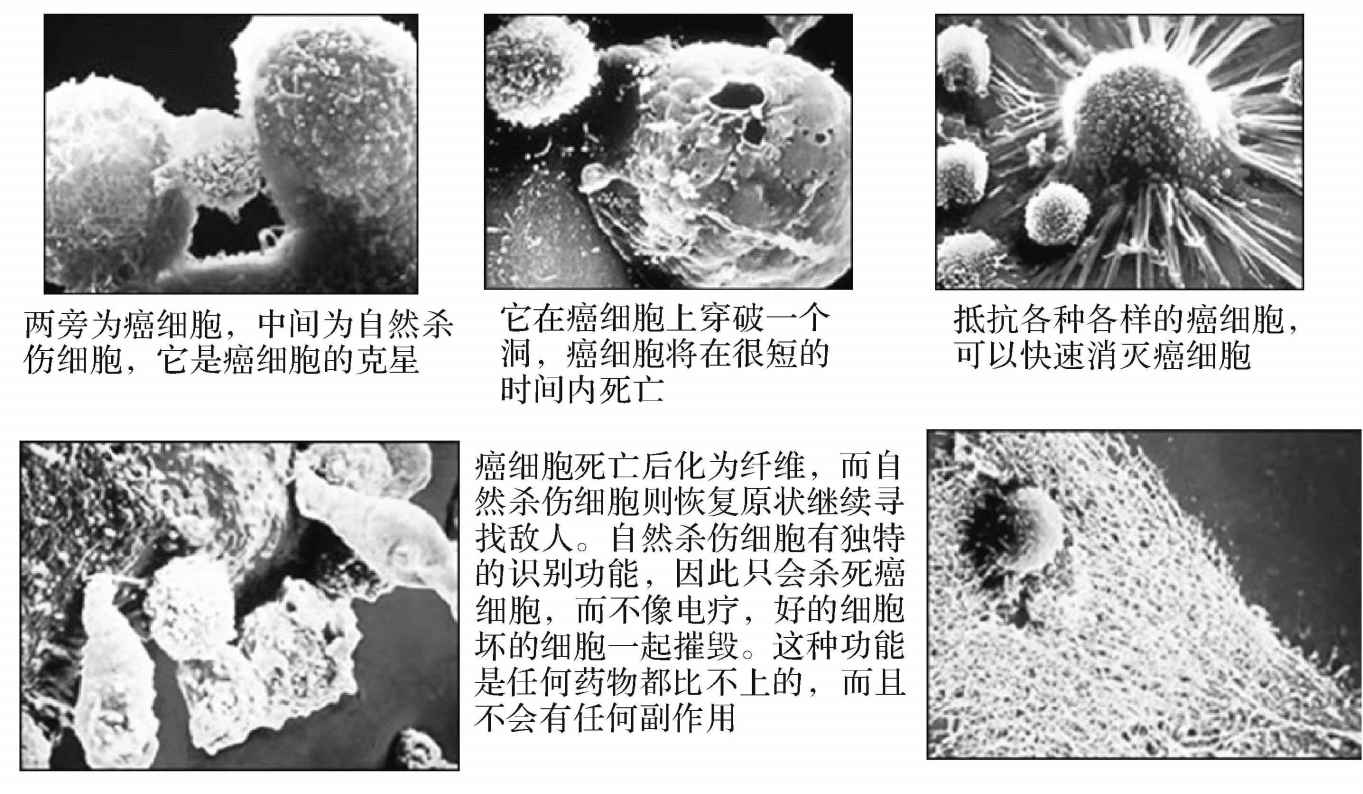
\includegraphics[height=0.2\textheight]{./images/Image00045.jpg}
    \captionsetup{justification=centering}
    \caption{NK细胞杀死癌细胞}
    \label{fig2-20}
\end{minipage}
\end{figure} 

1.来源及分布

NK细胞是由骨髓中的共同淋巴样祖细胞(commen lymphoid
progenitor,CLP)分化而来,其发育、成熟可能循骨髓途径或胸腺途径。人类和小鼠NK细胞主要分布于脾脏(占脾细胞总数3\%~4\%)和外周血(占淋巴细胞总数5%~7%),在淋巴结以及其他组织内(如肺脏等)也有少量NK细胞存在。近年发现,肝脏中NK细胞占淋巴细胞总数50\%以上,其生物学意义有待阐明。

2.功能

(1)能非特异性杀伤某些肿瘤细胞和病毒感染的靶细胞,具有抗肿瘤、抗感染的功能。

(2)NK细胞可产生IL-1、IFN-r、TNF等,有免疫调节作用。

(3)参与移植排斥反应、自身免疫病、超敏反应的发生。


\subsection{单核吞噬细胞系统}

单核吞噬细胞系统(mononuclear phagovyte
system,MPS)包括单核细胞、巨噬细胞,是体内具有最活跃生物学功能的细胞类型之一(图\ref{fig2-21})。

\begin{figure}[!htbp]
 \centering
 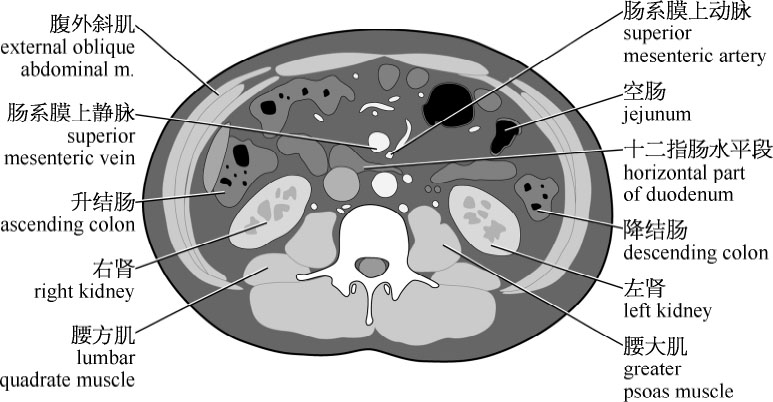
\includegraphics[width=.7\textwidth]{./images/Image00046.jpg}
 \caption{单核吞噬细胞}
 \label{fig2-21}
  \end{figure} 

1.表面标志:表达多种表面标志,并借此发挥各种生物学功能,如MHC分子、黏附分子等。这些表面标志不仅参与细胞黏附及对颗粒抗原的摄取、递呈,也介导相应配体触发的跨膜信号转导,并影响细胞分化和发育等。

2.产生多种酶及分泌产物:单核吞噬细胞能产生各种溶酶体酶、溶菌酶、髓过氧化物酶等,还能产生和分泌近百种生物活性物质,如细胞因子(IL-1、IL-6、IL-12等)、补体成分(C1、P因子等)、凝血因子,以及前列腺素、白三烯、血小板活化因子、ACTH、内啡肽等活性产物。

3.功能:具有抗感染、抗肿瘤、免疫调节的作用。


\subsection{其他免疫细胞}

(一)中性粒细胞

中性粒细胞表面具有IgFc受体和C3b受体,具有高度趋化性和非特异性功能,有抗感染作用(图\ref{fig2-22})。

\begin{figure}[!htbp]
 \centering
 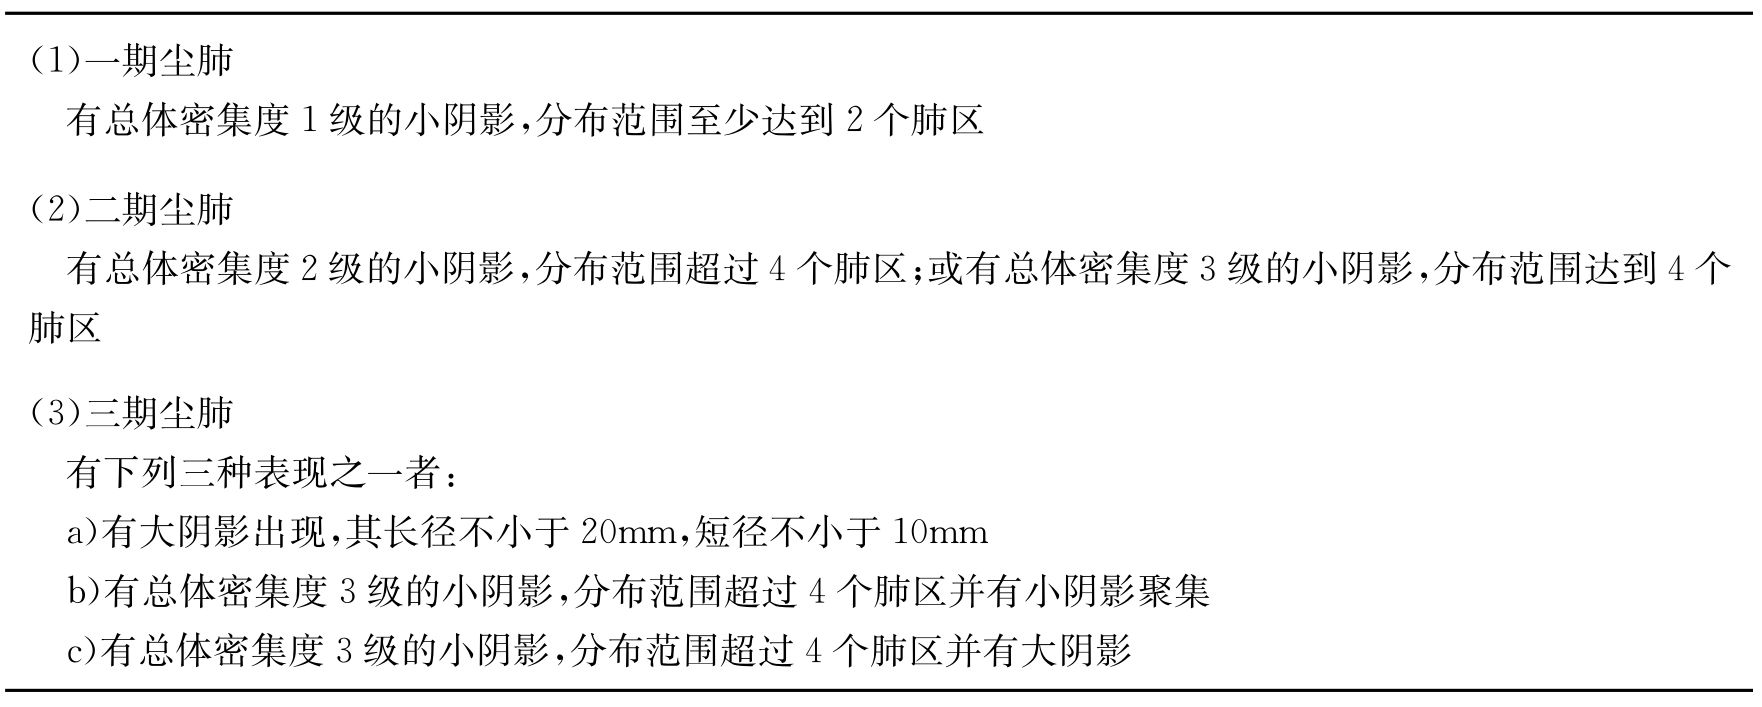
\includegraphics[width=.7\textwidth]{./images/Image00047.jpg}
 \caption{中性粒细胞的吞噬作用}
 \label{fig2-22}
  \end{figure} 

(二)嗜酸性粒细胞

嗜酸性粒细胞具有IgFc受体,参与IgE介导的ADCC效应;具有吞噬作用,抗寄生虫和对I型超敏反应的负调节作用。

(三)嗜碱性粒细胞与肥大细胞

嗜碱性粒细胞与肥大细胞表面具有IgE的Fc受体,能参与I型超敏反应、抗肿瘤作用(图\ref{fig2-23})。

\begin{figure}[!htbp]
 \centering
 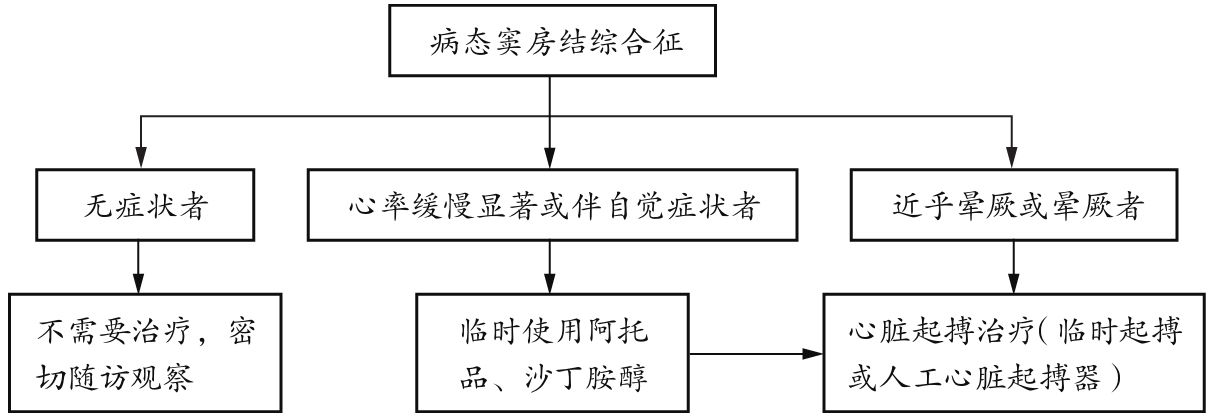
\includegraphics[width=.6\textwidth]{./images/Image00048.jpg}
 \caption{肥大细胞参与Ⅰ型超敏反应}
 \label{fig2-23}
  \end{figure} 

(四)红细胞

1.红细胞免疫的物质基础

① 红细胞CR1分子------结合C3b/C4b;

② 红细胞CD58分子------即LFA-3,与CD2互为配体和受体;

③ 红细胞CD59分子------阻止C9与C5B678结合,促进T细胞有丝分裂;

④ 红细胞CD55分子------即衰变加速因子DAF;

⑤ 红细胞CD44分子------参与T、B的分化、成熟、活化,细胞黏附;

⑥ 红细胞NK细胞增强因子------增强NK细胞的毒性;

⑦ 红细胞趋化因子受体------参与调控炎症反应。

2.红细胞在整体免疫反应中的作用

① 增强吞噬作用;

② 清除循环免疫复合物;

③ 识别和携带抗原;

④ 免疫调节作用;

⑤ 效应细胞的作用。

\section{思考练习与课外阅读}
\noindent\textbf{【理解与思考】}

1.你能向一位没有免疫学知识的人,形象地解说机体免疫系统的构成及其作用吗?

2.你能描绘出体内淋巴细胞的一生历程吗?

3.如果你是一病原微生物,进入机体后你能遭遇哪些危险?

4.如果你是一免疫细胞,你又是如何保证机体健康的?

5.以红细胞的口气,向别人叙述一下你在人体内的贡献。

\noindent\textbf{【课外拓展】}

1.白血病中,为何某一种白细胞数量过度增加?其分化机理如何?

2.淋巴细胞的阴性选择、阳性选择是如何进行的?有何意义?

3.造血干细胞的分化过程如何?在哪些因素作用下发生的?

4.与红细胞等比较,为何白细胞类都是“短命细胞”?

5.自然杀伤细胞在肿瘤防治中有哪些作用?目前用免疫的方法治疗肿瘤有哪些方法?

\noindent\textbf{【课程实验与研究】}

1.设计一个检测淋巴细胞活性的实验。要求分类定量。

2.设计一种诱导造血干细胞分化为NK细胞的实验方法。

3.白血病的种类有哪些?设计一种通过阻断细胞的分化途径来预防某种类型的白血病方案,并分析可行性。

4.设计一种方案,检测免疫细胞能释放哪些生物活性物质,并实施实验,完成实验报告。

5.设计检测饲喂蜂蜜对小鼠机体免疫力影响的三种以上指标,并设计实验方案,完成实验,写出小论文。

6.Nature最近报道发现“自然杀伤(NK)细胞的一个新亚类”,请问如何鉴别其为新的发现?

\noindent\textbf{【课程研讨】}

1.为何机体免疫细胞对自身的成分不产生排斥?

2.整个免疫系统与一个国家的防御力量有什么相似之处?请加以比较说明。

3.免疫系统与机体别的系统一样,各自负起使命,你认为机体是如何抵御病原微生物入侵的?如果病原微生物进入机体,机体又是如何清除的?

4.如何区别不同的淋巴细胞?

5.查阅资料,阐述淋巴细胞当今的研究进展。

\noindent\textbf{【课后思考】}

1.详细叙述免疫系统的构成及其作用。

2.骨髓、胸腺、淋巴结、脾脏的主要免疫功能。

3.T、B淋巴细胞的分类及其作用。

\noindent\textbf{【课外阅读】}

\begin{center}
\textbf{\Large 红细胞免疫发展史}
\end{center}

红细胞免疫和其他自然科学一样,它的发展也经历着三个阶段,即经验、实验、理论阶段。在发展中各阶段难以截然分开,反复循环,不断深入,不断提高。

\begin{center}
{\large 一、经验阶段}
\end{center}

我国劳动人民在长期与疾病的斗争中体会到血液的重要,往往将血与生命联系在一起,事实上血液特别是红细胞是机体生命活动的物质基础。祖国医学云:“气血是人体生命活动的物质基础”,“离开了气血,则整体不能联系,人身无有依附”。在20世纪初,Landsteiner
用免疫学方法在人类红细胞与血液混合实验中,观察到凝聚现象,后来通过多次反复试验观察,发现了人类ABO
血型系统,认识了红细胞表面存在许多能与血清中相应抗体凝集的抗原,如Mn、P
型、Rn、Lutheran、Lewis、Kell、Duffy、Kidd
等。除目前已知的数十种血型抗原外,发现红细胞还含有其他抗原。20世纪30年代,杜克(L
.H.Duke)首先发现锥虫在抗血清及补体存在时可黏附到人类红细胞上,推测在人的红细胞膜上存在有一种与免疫有关的物质。在临床上,人们对某些疑难病、原因不明性疾病等患者,采用输新鲜血液的办法,往往可得到满意的治疗效果。但究其原因,过去人们并不很清楚,自红细胞免疫问世以来,人们对上述现象的解释有了理论依据。如
G-BS
现已证实属红细胞免疫缺陷症;有些疾病,由于输注红细胞后,机体免疫功能得到了改善,即给了机体以
“气血”,“气血相依,循环不已”,“防治百病莫不以气血为本”。

\begin{center}
{\large 二、实验阶段}
\end{center}

实验阶段即将人们观察到的现象,进行科学实验的过程。1953年,R.A.Nelson用正常人的红细胞、白细胞与相应抗体致敏的
I
型肺炎双球菌进行培养,发现肺炎双球菌可黏附于正常人的红细胞表面并被白细胞吞噬,其吞噬率可达60\%,远远高于未加相应抗体组和未加相应红细胞组,作者推测红细胞膜存在免疫黏附受体,将此命名为免疫黏附现象。1963年,Nishioka证实红细胞这种免疫黏附现象是通过红细胞膜
C3受体实现的。1980年,Fearon从红细胞膜分离到这一受体,并详细研究了CR1的性质,是分子量190
000~250
000的多态性膜糖蛋白。1986年,郭峰通过体外对比实验证明红细胞可黏附补体调理过的各种肿瘤细胞,并发现红细胞可黏附未经调理过的肿瘤细胞,其机理不明。1992年,刘景田等证实这种直接免疫黏附的机理与红细胞上
CR1 和肿瘤细胞上 C3b分子有关。

\begin{center}
{\large 三、理论阶段}
\end{center}

1981年,美国生殖免疫学家Siegel在前人研究的基础上发现红细胞有多种免疫功能,红细胞可黏附胸腺细胞,并发现血清中存在有红细胞免疫黏附抑制因子,预见了血清中存在有红细胞免疫调节系统,推测红细胞在阻止肿瘤细胞血行转移中有作用。他综合看待以往对红细胞免疫的研究成果,提出了
“红细胞免疫系统” 的新概念,冲破了传统上划分血细胞功能的
“界限”,更新了人们对红细胞功能的认识。20 世纪 80
年代,我国学者郭峰教授在红细胞免疫的基础理论和应用研究方面取得了许多突破性进展,如发现血清中存在有红细胞免疫黏附促进因子、红细胞有增强各类免疫细胞的免疫功能,建立了许多红细胞免疫功能的监测方法等,大大推动了我国红细胞免疫的发展。1994
年,刘景田在证实血清中确实存在有正负两种红细胞调节因子的基础上,发现了这两种因子对粒细胞、淋巴细胞(主要指B
淋巴细胞)都有相同调节作用,推测这种因子对具有
CR1的细胞都有调节作用,故将这种因子称为 CR1 免疫调节因子(Complement
recepor 1 immuneregalation factors,CR1FR)。其中具有正调节作用者称为
CR1免疫黏附促进因子(Complement recepor 1 immune regalation enhance
factors,CR1FER);具有负调节作用者称为 CR1 免疫黏附抑制因子(Complement
recepor 1 immune regalation inhibitor factors,CR1FIR)。

(资料来源:刘景田,党小军.红细胞作为免疫细胞的事实及意义[J].深圳中西医结合杂志,2002,12(1):10-12)

\begin{center}
\textbf{\Large 红细胞免疫功能研究进展}
\end{center}

红细胞是血液中最主要的细胞成分。传统认为,红细胞结构简单,功能单一,仅运输氧和二氧化碳。随着科技的发展,人们对红细胞免疫功能的认识不断深入。1930年,Duck发现人类红细胞膜上存在与免疫有关的物质;1953年,Nelson首次提出红细胞不仅具有免疫黏附功能还能促进白细胞的吞噬作用;1963年,Nishioka证实红细胞免疫黏附的物质基础是红细胞膜上补体C3b受体(C3breceptor,C3bR);1980年,Fearon进一步从红细胞膜上分离出受体CR1(complementreceptor1,CR1)。1981年,Siegel在前人研究的基础上提出了“红细胞免疫系统(redcellimmunesystem,RCIS)”新概念,成为红细胞免疫研究的里程碑,促进了红细胞免疫研究工作的迅速发展。医学工作者研究发现,红细胞具有很多与免疫有关的物质,包括补体受体CR1、CR3、淋巴细胞功能相关抗原-3(CD58)、CD44、人类补体膜辅助因子蛋白(MCP)、降解加速因子(DAF)、过氧化物歧化酶(SOD)、阿片肽受体、NK细胞激活因子(NKAF)以及红细胞趋化因子受体等。红细胞不仅具有识别、存储、递呈抗原,清除免疫复合物,促进吞噬细胞功能等作用,自身还存在完整的自我调节控制系统,是机体免疫系统的重要组成部分。

\begin{center}
{\large 一、红细胞免疫功能的分子学基础}
\end{center}

1981年,Siegel提出了“红细胞免疫系统”概念,并指出红细胞免疫黏附(redcellimmuneadhesion,RCIA)是红细胞发挥免疫功能的主要手段,RCIA的分子基础则是红细胞膜上的补体受体(complementreceptor,CR)。目前,已明确红细胞膜上的补体受体有I型(CR1)和Ⅲ型(CR3),主要为CR1,其基因结构、分子结构及生物学功能已部分明确。CR1属于补体调控蛋白,分子量为160~260kd,是一种单链膜结合蛋白,能与补体系统中C3b、C4b高亲和性地结合。就单个红细胞而言,膜上CR1受体密度仅为白细胞110~150,但红细胞数量庞大,在体内约90\%C3b受体存在于红细胞膜上。CR1与血液循环中带有C3b的免疫复合物(immnunecomplex,IC)结合,并运送至肝脏及脾脏内皮系统予以清除,即为红细胞免疫黏附(RCIA)机制。随着国内外研究的深入,发现CR1参与机体免疫功能的机制远比上述复杂得多。红细胞能携带抗原抗体复合物,还能主动地将抗原抗体复合物传递给单核巨噬细胞并使之激活,增强单核巨噬细胞对抗原抗体复合物的摄取并加工递呈给T细胞。此外红细胞在类孢子病、溶血性贫血、病毒性肝炎、系统性红斑狼疮、肾病、疟疾等疾病中的作用也得到证实。红细胞上CR1表达降低或红细胞黏附功能下降会引起机体免疫功能低下,研究红细胞CR1介导的免疫黏附功能对评价机体天然免疫功能状况乃至特异性细胞或体液免疫可能都具有十分重要的意义。目前,CR应用热点是对双特异性单抗异聚体(heteropolymer,HP)的研究。Taylor以红细胞CR1分子为桥梁,建立了抗CR1单抗与抗致病原单抗交叉连接的HP清除循环中致病原的方法,引起了广泛关注。HP结合红细胞时,还可结合循环中病原体,形成异聚体复合物(E-HP-Ag),并迅速将EHPAg移至肝脏彻底销毁,红细胞本身数量却无减少。此外可溶性CR的应用也有所突破,Yazdanhakhsh等报道使用基因重组的可溶性CR1在动物实验中成功阻断了补体活化。

\begin{center}
{\large 二、红细胞免疫功能}
\end{center}

(一)清除循环免疫复合物

研究表明,红细胞膜上补体受体具有免疫黏附、携带及清除循环液相中抗原异物的功能,清除循环免疫复合物(circleimmunecomplex,CIC)是红细胞主要的免疫功能。目前认为,大多数C3b-免疫复合物(C3b-IC)通过CR1连接。CR1存在于红细胞、多形核白细胞、巨噬细胞及淋巴细胞的膜表面。红细胞膜上CR1分布有两种形式:散在和集簇分布。约50\%红细胞膜上CR1呈集簇分布,多形核白细胞上CR1集簇分布率小于15\%。CR1集簇分布方式使它与C3b-IC的结合位点呈多价性,连接更牢固。实验证明,单个白细胞表面CR1受体较红细胞多,但在细胞浓度相同时,两种细胞的免疫复合物结合率相同。血液中红细胞总数远远超过白细胞,循环系统中约95\%C3b受体位于红细胞上,与CIC结合机会为白细胞的500~1000倍。因此,体内清除CIC起主要作用的是红细胞,不是白细胞。Nedaf体外实验结果证明了这一推测。红细胞清除免疫复合物的机理是:红细胞通过表面CR1受体与循环中C3b-IC结合(即发生黏附),形成的复合物被血流带到肝、脾等器官,这些器官的固定吞噬系统捕获红细胞结合的IC,通过巨噬细胞膜表面的Fc受体与IC中的抗体Fc段结合,此时红细胞从IC上解离,再度进入循环,而捕获IC的巨噬细胞则通过膜表面CR1受体再与IC补体C3b结合,Fc受体与CR1受体的协同作用使巨噬细胞的吞噬作用加强,而将IC吞噬并清除到体外。Sherwood实验研究发现:红细胞表面所黏附的循环免疫复合物被转运到吞噬细胞,吞噬细胞所接受CIC的多少与红细胞CIC的浓度呈平行关系,红细胞无任何损伤或被吞噬。有实验证明,肝脏内巨噬细胞表面的Fc受体和CR1受体密度较高,且Fc受体比红细胞膜上CR1受体活性强,致使肝、脾内巨噬细胞对免疫复合物(IC)有更强的作用,可以从CR1密度低的红细胞上夺取IC。

(二)增强吞噬细胞的吞噬功能

1953年,Nelson将经抗体、补体调理过的肺类球菌复合物注入猴体,发现球菌几乎全部黏附于红细胞上。实验证明,血浆中被红细胞黏附的复合物(IC)较未被黏附的更容易被吞噬。1982年,Forslod进一步证实了上述现象作用机理,用C3b及IgG(兔抗酵母菌IgG)调理过的酵母菌与吞噬细胞一起孵育,加入红细胞后,吞噬细胞对酵母菌的吞噬率比未加入红细胞组增加了34\%;给予红细胞溶解产物后,吞噬率增加75\%。用过氧化氢酶及超氧化物歧化酶代替红细胞后,吞噬率增加程度相似。可能是红细胞首先黏附酵母菌,然后红细胞酵母菌复合物与吞噬细胞作用,红细胞内含有高浓度的过氧化氢酶(Cat)及超氧化物歧化酶(SOD),并具有强力的抗氧化作用,清除吞噬过程中产生的氧化代谢产物(ROM),促进吞噬作用。近年来,人们将红细胞作为SOD的载体以延长其在体内的存活时间,提高血液相容性,防治缺氧、缺血过程中活性氧造成的组织损伤,取得了良好的效果。

(三)对T淋巴细胞和淋巴因子的调控作用

实验表明,红细胞通过CD58、CD59与T辅助细胞CD2的黏附激活T淋巴细胞免疫功能,与B细胞作用亦能促使增殖、分化产生免疫球蛋白。红细胞还可调控淋巴细胞产生γ-干扰素,增加淋巴细胞转化率和培养液中IgG、IgA的含量。CD58分子即淋巴细胞功能相关抗原23(LFA-3),是一种分子量为55~70kd的糖蛋白,属于免疫球蛋白超家族成员,广泛表达于人体内各种免疫细胞和红细胞上,结构与CD2(LFA-2)相似,故CD58与CD2分子可以相互结合。表达CD58抗原递呈细胞(APC)或靶细胞通过与表达CD2分子的T细胞相互黏附,促进T细胞识别抗原,CD58与CD2结合后又参与细胞信号转导,此信号为T细胞活化的一种重要协同(辅助)刺激信号。相对于T细胞活化时TCR识别性结合MHC一抗原肽复合物的T细胞活化第一信号,CD58与CD2的结合又被称为T细胞活化第二信号。有证据表明,结合抗原抗体复合物(IC)的红细胞通过膜表面CR分子介导的免疫黏附作用将免疫复合物传递给巨噬细胞,又经膜表面CD58分子与辅助性T细胞膜表面CD2分子结合间接起到类似于抗原递呈细胞(antigenpresentingcell,APC)的递呈抗原作用,促进外周血T细胞活化与细胞周期改变,从而间接调控免疫应答。CD59分子即攻膜复合体(membraneattackcomplex,MAC)抑制物,是一种分子量为18~20kd的糖蛋白。CD59可阻碍C7、C8与C5b~6复合物结合,抑制MAC形成。CD59除广泛参与补体调节,还能与CD2分子结合,是继CD58之后发现的又一CD2配体。CD59与CD2结合也能发挥类似CD58与CD2结合的协同刺激信号的作用,CD58和CD59与T细胞黏附时具有协同作用,同时表达CD58与CD59的靶细胞更有利于T细胞的激活。近年来的研究发现,CD59缺陷还常伴随CD55缺陷,提示其功能可能为一种广泛参与红细胞免疫调节的协同蛋白。

(四)识别、储存和递呈抗原

红细胞对自我和非我抗原具有识别功能,且具有储存抗原的能力。1982年Garvey将\textsuperscript{3}
H标记的牛血清清蛋白(BSA)注入新生兔,放射自显影发现外周血液和肝血管内红细胞表面均黏附有\textsuperscript{3}
HBSA,并持续存在4~6周以上。若将兔血清清蛋白注入新生兔体内,则不出现上述现象,由此证实了上述观点。红细胞的抗原递呈能力表现为红细胞免疫黏附特性具有双重性,即红细胞上CR1与IC相黏附时,可同时黏附自身胸腺细胞和T细胞,形成自身玫瑰花环,IC中抗原与T淋巴细胞紧密靠拢,红细胞将抗原递呈给T淋巴细胞,使其俘获抗原能力增强,从而增强了免疫应答。

(资料来源:夏佐中.红细胞免疫功能研究进展[J].重庆医学,2008,37(20):2365-2367)

\begin{center}
\textbf{\Large 天然免疫反应需要T细胞参与}
\end{center}

先天性免疫和获得性免疫虽是不同的概念,具有不同机制,但在对付入侵的病原体时,它们并不各自为政或分庭抗礼,而是互相配合协同作战的。例如,当伤寒杆菌侵入后,首先由先天性免疫(如补体、吞噬细胞等)对付,等到体内产生抗伤寒抗体和免疫淋巴细胞(获得性免疫因素),就与补体和吞噬细胞(先天免疫因素)协同作用,清除体内伤寒杆菌。

2009年1月,中科院生物物理所感染免疫中心唐宏研究员和傅阳心教授在《免疫学趋势》(Trends
in Immunology)杂志上以《Do adaptive immune cells suppress or activate
innate
immunity》为题,系统阐述了他们近来提出的“天然免疫反应需要T细胞参与”的新理论。经典的免疫学理论认为,天然免疫反应启动获得性免疫,而获得性免疫随后进一步放大天然免疫效应,二者的合作与平衡才能清除入侵病原,起到免疫保护的作用。该实验室近期的研究结果表明(原文见Nature
Medicine,2007;Nature Reviews in Immunology,2007; Nature
China,2008),原先关于区分天然免疫和获得性免疫的界限可能并不那么清楚,T细胞其实也参与天然免疫反应并维持其稳态。经典理论认为天然免疫和获得性免疫反应的双重低下是早产儿容易死于急性感染的主要原因。该实验室的研究发现,实际上,在感染早期获得性免疫细胞对于天然免疫反应具有负调控的作用,从而有效地将天然免疫反应的强度控制在一定的水平内而不至于对机体造成免疫损伤。新生鼠或早产儿由于获得性免疫低下,天然免疫炎性反应无法得到有效控制,这种“炎性因子风暴”才是致死原因。因此,获得性免疫一方面抑制感染早期的炎症反应,另一方面在感染后期行使病原特异性清除功能,两者缺一不可。

这个新理论对于深入了解病毒性感染的炎症反应和病毒清除机理,控制免疫低下病人(新生儿、老年人、放化疗癌症病人、器官移植患者或艾滋病人)机会性感染具有极高的指导价值。

(资料来源:http://www.bioon.com/biology/Immunology/383575.shtml)

\begin{center}
\textbf{\Large Immunity:嗜中性粒细胞通过群集抵抗寄生物}
\end{center}

嗜中性粒细胞在抵抗病原体的免疫响应中扮演了一个重要角色,但是它们调节自身保护效应的机制却一直没有搞清。最近发表在《免疫学》上的一项研究显示,在嗜中性粒细胞转移到淋巴结的过程中------它们在这里形成了动态分子团,就像蜂群一样,这些细胞扮演了抵抗胞内寄生物的一个重要角色。

为了研究嗜中性粒细胞与淋巴结之间的关系,美国加利福尼亚大学伯克利分校的Tatyana
Chtanova等使用了嗜中性粒细胞表达绿色荧光蛋白质的小鼠,并使它们传染上胞内寄生物------弓形虫,同时利用荧光显微镜方法检测淋巴结组织切片。研究人员观察到,在感染后,嗜中性粒细胞迅速转移到淋巴结中,并且这一过程依赖于它们的适应物蛋白质MyD88(骨髓差别主要响应基因88)的表达。此外,渗透的嗜中性粒细胞被发现形成了群集,并且这些群集与寄生虫在淋巴结中所处的位置相符合。

利用完整无损的淋巴结的双光子激光扫描显微镜,研究人员随后调查了嗜中性粒细胞群集形成的动力学原因。他们观察到,在被弓形虫感染后,嗜中性粒细胞形成两种群集:瞬时群集,即规模较小且溶解迅速;持久群集,即规模较大(由于嗜中性粒细胞的连续转移和与附近群集的合并)且在成像期间内持续存在。基于这些,研究人员推断,一旦一个群集达到一定的规模,由嗜中性粒细胞产生的信号将会压倒周围群集的信号,形成一个稳定的群集中心。嗜中性粒细胞同时被发现以直接的方式以及一连串地向这些群集迁移,这意味着这里的细胞之间可能存在着信息传递。

研究人员继续研究了群集如何在感染后被组合起来,并且观察到它们能够被嗜中性粒细胞与从淋巴结被感染的细胞中溢出的寄生虫之间的合作行为所激活。更特别的是,小分子团最初是由少数“先驱”嗜中性粒细胞所形成的,并且这些分子团诱导其他细胞向群集中迁移。

一个嗜中性粒细胞已知能够通过分泌酶使组织退化,研究人员随后调查了是否群集的出现与淋巴结中被感染细胞的破坏相一致。实际上,他们观察到,CD\textsuperscript{+}
\textsubscript{169}
巨噬细胞的连续层------通常被发现在淋巴结的囊下窦------在被弓形虫传染后被破坏,这一区域的缺口与嗜中性粒细胞群集的位置相一致。这意味着,随着寄生虫的传染,嗜中性粒细胞群集通过除去囊下窦巨噬细胞从而破坏了淋巴结的结构。

研究人员认为,这些数据表明,寄生虫在从被感染的细胞中游出的过程中所释放的信号,以及由先驱嗜中性粒细胞导致的动态群集的形成,去除了淋巴结囊下窦中被感染的巨噬细胞。

(资料来源:Immunity,19 September 2008
doi:10.1016/j.immuni.2008.07.012)

\begin{center}
    \textbf{\Large Nature:发现NK细胞新特征}
\end{center}

加州大学微生物免疫系与癌症研究中心的研究人员发现自然杀伤细胞的一种新的特征,这一成果公布在1月11日Nature在线版上。

自然杀伤细胞(natural killer
cell,NK)是机体重要的免疫细胞,不仅与抗肿瘤、
抗病毒感染和免疫调节有关,而且在某些情况下参与超敏反应和自身免疫性疾病的发生。由于NK细胞的杀伤活性无MHC限制,不依赖抗体,因此称为自然杀伤活性。
NK细胞胞浆丰富,含有较大的嗜天青颗粒,颗粒的含量与NK细胞的杀伤活性呈正相关。NK细胞作用于靶细胞后杀伤作用出现早,在体外1小时、体内4小时即可见到杀伤效应。NK细胞的靶细胞主要有某些肿瘤细胞(包括部分细胞系)、病毒感染细胞、某些自身组织细胞(如血细胞)、寄生虫等,因此NK细胞是机体抗肿瘤、抗感染的重要免疫因素,也参与第Ⅱ型超敏反应和移植物抗宿主反应。

在获得性免疫应答机制中,感染发生后未致敏的T细胞会开始复制增殖,免疫系统会生成具有长期记忆性的细胞,在经历第二次相同病毒的感染时,免疫细胞就能迅速地调动起来,发挥免疫功能。

在现在的理论中,自然杀伤细胞被归为天然免疫细胞,它与细胞毒性T细胞具有诸多相似的特点。研究者以小鼠为模型,让其感染巨细胞病毒,与细胞毒性T细胞相似的特性出现了,脾脏中表达病毒特异性的Ly49H受体的自然杀伤细胞数量增高100倍,在肝脏中高达1000倍。经历收缩期后,Ly49H阳性的自然杀伤细胞定居在淋巴组织或是非淋巴器官中长达数月之久。这些能自我更新的有记忆性的自然杀伤细胞再次遭遇相同的病原后能迅速反应,脱颗粒,释放细胞因子发挥免疫功能。如果将这些有记忆性的自然杀伤细胞转移到年幼的动物体内,自然杀伤细胞能在年幼动物首次遭遇相应病原的时候发挥杀伤作用,也就是说这些记忆性的自然杀伤细胞能拿来即用。

这些研究结果证明,自然杀伤细胞其实不仅是天然免疫系统中的重要作用成分,它同样具有获得性免疫细胞的一些特征(有记忆性)。

研究者认为,在免疫系统中,NK细胞反应的速度比T细胞或B细胞要快,因此,NK细胞的这种记忆性能可能有助于设计更有效、反应更迅速的疫苗。

(资料来源:Nature advance online publication 11 January
2009|doi:10.1038/nature07665)

\begin{center}
\textbf{\Large 发现嗜酸性粒细胞对免疫系统发育有重要作用}
\end{center}

澳大利亚Alberta大学研究人员发现在免疫发育过程中,嗜酸性粒细胞(eosinophil)有重要的作用。这项研究结果发表在11月版的《American
Journal of Pathology》杂志上。

当免疫系统对环境中无害的物质如花粉或霉菌产生不正常应答时,常常导致哮喘或过敏性疾病发生。常见的过敏性疾病有湿疹、荨麻疹、花粉热、哮喘、食物过敏等。

根据接受刺激后产生炎症的类型和分泌物,可以将免疫应答分为Th1型和Th2型。Th1免疫应答一般针对细胞内感染,如细菌或病毒感染。而Th2免疫应答则针对较大的寄生虫,如线虫感染。而哮喘和过敏性疾病通常是由于产生了不正常的Th2免疫应答。

虽然嗜酸性粒细胞作为一种免疫细胞,一直被认为可以调节过敏反应以及哮喘Th2免疫应答,同时也可能是控制Th1
和Th2免疫应答的重要开关。因此,研究人员对儿童胸腺中嗜酸性粒细胞发育进行研究。胸腺是人体的免疫器官,也是早期Th1/Th2分化的场所,随着年龄的增长会逐渐萎缩。研究表明,胸腺IDO\textsuperscript{+}
嗜酸性粒细胞(Thymic Indoleamine 2,3-Dioxygenase Positive
Eosinophils)在人类婴儿期或许对Th2免疫应答具有免疫调节作用。

(资料来源:http://www.med66.com/new/27a562a2009/20091111dongni9540.shtml)

\begin{center}
\textbf{\Large T细胞记忆机制}
\end{center}

澳大利亚国立大学医学研究所、化学研究所的科学家发现新的免疫理论,相关成果公布在最新一期的Immunity上,并列为封面文章。

众所周知,B细胞具有记忆性,一般来说B细胞的记忆性的形成与DNA序列的改变有联系,B细胞通过改变DNA序列来维持细胞的记忆性。但是,免疫细胞的记忆性机制研究比较多的是B细胞,相比之下,T细胞研究比较少。

研究小组发现,记忆性T细胞的分化过程中,RNA重排起重要作用。研究小组以小鼠的研究模型,通过沉默一个记忆性T细胞分化的关键基因ptprc(是产生记忆性T细胞CD45RO的重要基因),结果发现记忆性T细胞的比例发生改变,并且RNA结合蛋白hnRNALL发生改变,会导致RNA的识别区域变得不稳定。

研究者发现,hnrpll突变会导致T细胞不在外周淋巴结聚集,但不影响增殖。对这些突变细胞进行外显子检测分析,结果发现记忆性T细胞的mRNA连接过程发生广泛的改变,并且相同的变化还出现在神经组织中,这可能是引发记忆性T细胞发生变化的原因。

(资料来源:Immunity,19 December 2008
doi:10.1016/j.immuni.2008.11.004)

\begin{center}
\textbf{\Large 发现参与免疫细胞形成的关键因子MAZR}
\end{center}

奥地利研究人员日前报告说,他们发现了参与免疫细胞------T细胞形成的一种关键因子。这一研究成果刊登在新一期英国《自然•免疫学》杂志上。

T细胞是淋巴细胞的一种,在免疫反应中扮演着重要角色。按照功能的不同,T细胞可以分成细胞毒T细胞和辅助T细胞等很多种类。其中细胞毒T细胞能够消灭感染细胞,而辅助T细胞可通过增生扩散来激活其他可产生直接免疫反应的免疫细胞。细胞毒T细胞和辅助T细胞都产生于共同先驱细胞,即双阳性胸腺细胞。

维也纳医科大学病理生理学专家维尔弗里德•艾梅尔领导的研究小组发现,一种名为MAZR的转录因子参与了双阳性胸腺细胞、细胞毒T细胞以及辅助T细胞的形成过程。

艾梅尔说,如果MAZR缺失,双阳性胸腺细胞就会转化成辅助T细胞,反之就会形成细胞毒T细胞。

(资料来源:Nature Immunology doi:10.1038/ni.1860)

\begin{center}
\textbf{\Large NK细胞敌我识别机制}
\end{center}

人体中的NK(Natural
killer)细胞可自行识别并杀死发生病变的细胞,英国一项最新研究揭示了这种免疫细胞的敌我识别机制,解答了长期以来人们对其作用机制的疑惑。

英国帝国理工学院的研究人员在新一期美国《公共科学图书馆•生物卷》月刊上报告说,他们使用高速显微镜成像技术,观测到NK细胞对所捕获细胞作出“杀与不杀”抉择的全过程。

报告说,NK细胞表面有许多受体感应器,这些受体分为“激活”和“抑制”两种。当它在人体内捕获一个可疑细胞后,两种受体将传回不同的信号,如果是病变细胞,“激活”信号大大增强,免疫细胞的“杀手本能”将被激活,从而杀死病变细胞;反之,如果捕获的是一个健康细胞,“抑制”信号将占主导地位,该细胞将会被释放。

NK细胞在杀伤靶细胞时不需要抗体参加,也不需要抗原预先致敏。此前人们已经知道它能够在病变细胞和健康细胞之间作出“杀与不杀”的抉择,但并不了解其作用机制。

(资料来源:PLoS Biol 7(7):
e1000159.doi:10.1371/journal.pbio.1000159)

\begin{center}
\textbf{\Large Th17细胞在免疫反应中的作用}
\end{center}

来自上海葛兰素史克研究中心与美国Baylor医学院的科学家最近在Th17的研究方面取得新的进展,相关成果文章公布在最新一期的《Nature
Medicine》上。

2005年,Th17概念提出,由于其表达的细胞因子和生物学功能、分化过程完全不同于Th1、Th2细胞,且Th17在慢性感染和自体免疫疾病过程中发挥重要的作用,因此,一经发现Th17就引起了研究者们浓厚的兴趣。

Th17细胞能够分泌产生IL-17A、IL-17F、IL-6以及肿瘤坏死因子α(tumor
necrosis factor
α,TNF-α)等,其功能主要体现在它分泌的这些细胞因子集体动员、募集及活化中性粒细胞的能力上。Th17细胞产生的最重要的效应因子是IL-17,其受体在体内广泛表达。虽然Th17细胞在自身免疫病中的病理性作用得到了证实,但研究者们认为这并不是它们的主要的原始功能。当出现感染或炎症等严重伤害的早期,机体都需要中性粒细胞参与阻止组织坏死或者脓血症。而Th17细胞产生的IL-17能有效地介导中性粒细胞动员的兴奋过程,从而有效地介导了前炎症反应。

研究发现,过量的Th17细胞会引发严重的自体免疫疾病,比如多发性硬化症(multiple
sclerosis)。了解Th17在自体免疫疾病的发生发展过程中的作用机制对治疗自体免疫疾病具有重要的意义。

Jingwu
Zhang等人发现,一种关键的细胞因子IL-7是维持Th17细胞存活与扩散的关键因子。他们研究发现,用IL-7受体拮抗剂可有效地抑制多发性硬化症的发病过程,经过IL-7受体拮抗剂的应用,过量的Th17细胞更易进入凋亡状态,有助于减少有害的Th17细胞。

研究人员深入地分析IL-7与IL-7R(IL-7
receptor)对Th17发育的关键机制。他们发现,患有实验性自身免疫性脑脊髓炎的小鼠与患有多发性硬化症的人类在接受IL-7后Th17细胞的数量显著增多。

而,对小鼠或是人类给予IL-7R拮抗剂治疗后,分化后的Th17细胞变得更易进入细胞凋亡程序,这可以有效地缓解自体免疫疾病的发展过程。

研究者还发现IL-7对其他类型的辅助性T细胞和调节性T细胞没有类似的功效。

研究者认为,IL-7可能是治疗多发性硬化症的一个潜在靶位。

(资料来源:Nature Medicine 10 January 2010 \textbar{}
doi:10.1038/nm.2077)


\chapter{胆道影像解剖}

胆道包括肝内外胆管、胆囊、胆囊管以及胰管等一系列管道结构,它是胆汁和胰液运输至十二指肠的管道,了解正常胆道结构具有十分重要的意义。

\section{检查方法}

诊断胆胰疾病的影像学检查手段有常规X线、超声、CT、血管造影和MRI等,各种检查方法各有其临床使用特点和限度。超声在临床上常作为胆系疾病诊断的首选检查方法,CT与超声相结合能对大多数胆胰疾病作出正确诊断。磁共振水成像技术是近年来磁共振成像重大进展之一,其中以磁共振胆胰管成像(MR
cholangiopancreatography,MRCP)应用最早、最广泛。MRCP自20世纪90年代初德国学者首次提出并应用以来,引起了广泛的关注,是一种发展较快,简便、安全、有效的观察胆胰管系统解剖和诊断胆胰管疾病的影像学检查技术,临床上可作为诊断胆胰管疾病的初筛检查手段。MRCP不需特殊的插管技术,也不必注射造影剂,是一种无创伤性检查,兼有横断面成像和造影检查的长处,既可提供与超声和CT相似的信息,又具有与ERCP类似的造影图像。MRCP与ERCP起着互补的作用,当上消化道手术和改建后,或食管、十二指肠严重狭窄时难以插管,不能作ERCP,这些病例就只能作MRCP检查。MRCP是利用胰液、胆液这些天然的对比剂,通过重建图像后处理,突出含液体的胆胰管结构影像。MRCP技术包括梯度回波(GRE)、快速自旋回波(TSE)以及由其衍化而来的快速采集驰豫增强(RARE)和单次激发快速自旋回波半傅立叶采集序列,采用最大信号强度(MIP)作三维立体重建,可显示胆系全貌,运用工作站中三维成像的连续性和旋转功能可显示胆胰管关系,并可直接观察病变形态,最后结合常规MR图像作出综合诊断。

\section{重建影像}

目前对于胆道最有效的无创成像方法就是MRCP,以下2幅图像即为MRCP图像。由于正常人胰管较细,因此部分正常人的胰管在MRCP上无法显示。
\begin{figure}[!htbp]
 \centering
 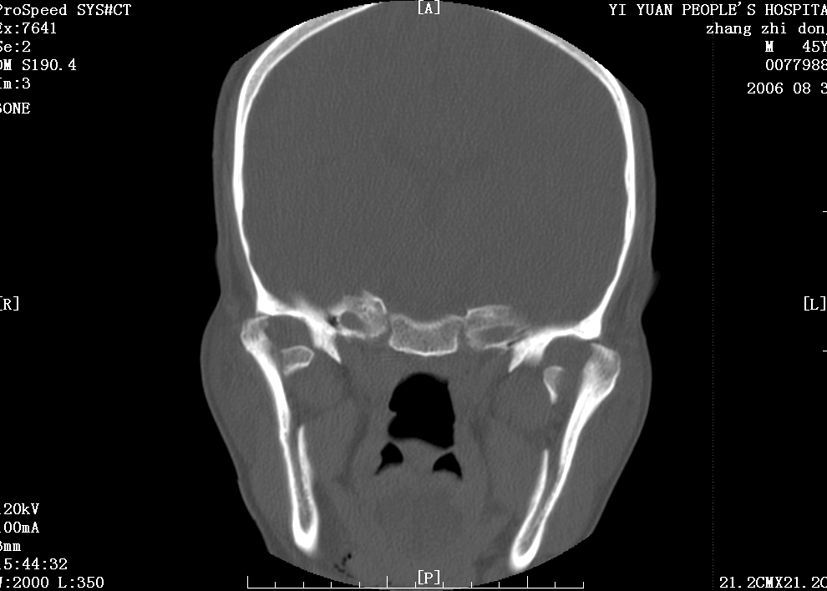
\includegraphics{./images/Image00164.jpg}
  \end{figure} 
 \FloatBarrier

\begin{figure}[!htbp]
 \centering
 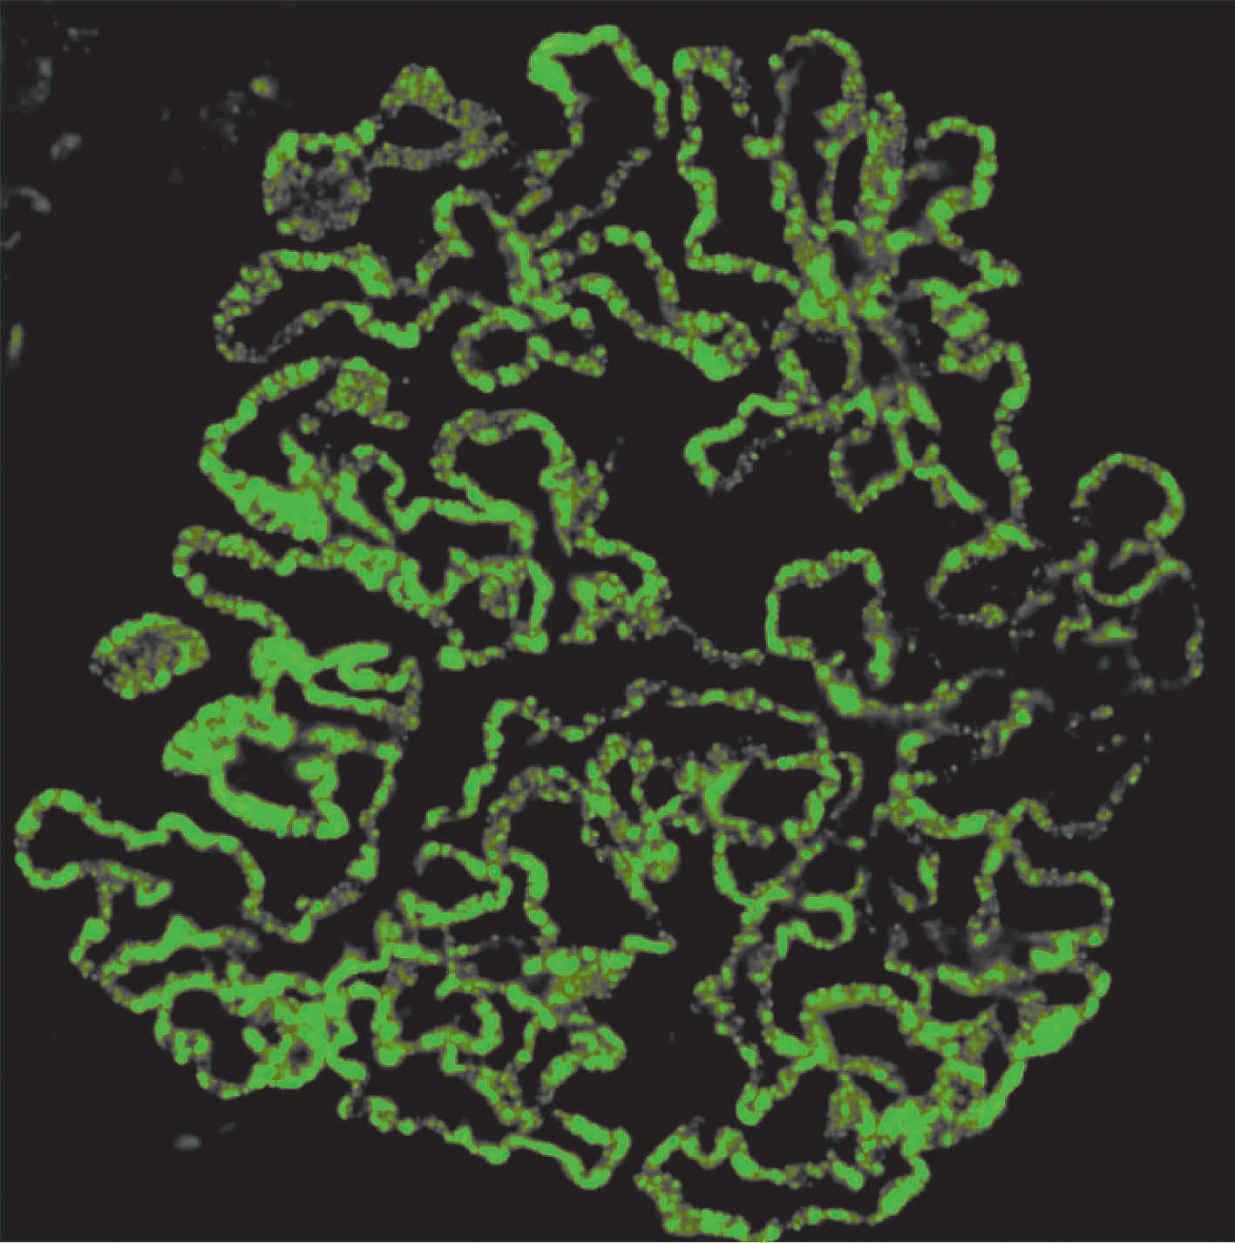
\includegraphics{./images/Image00165.jpg}
  \end{figure} 
 \FloatBarrier


\chapter{咯 血}

\section{12 咯血}

咯血是指喉及喉以下呼吸道或肺组织任何部位的出血,经口腔咳出者。咯血大多数为呼吸系统及(或)循环系统疾病所致,口腔、鼻腔或上消化道的出血有时易和咯血混淆。鼻腔出血多从前鼻孔流出,并常在鼻中隔前下方发现出血灶,较易诊断。有时鼻后部的出血量较多,特别是在睡眠时不自觉地坠入气道而于清晨咳出,较易误诊为咯血;如见血液从后鼻孔沿软腭或咽后壁下流,用鼻咽镜检查可以确诊。此外,还须检查有无鼻咽癌、喉癌、口腔溃疡、咽喉炎及牙龈出血的可能性。

呕血为上消化道出血,经口腔呕出,出血灶多位于食管、胃及十二指肠。咯血和呕血可根据病史、体征及其他检查方法进行鉴别,参见表\ref{tab4-1}。

\begin{table}[htbp]
\centering
\caption{咯血与呕血的鉴别}
\label{tab4-1}
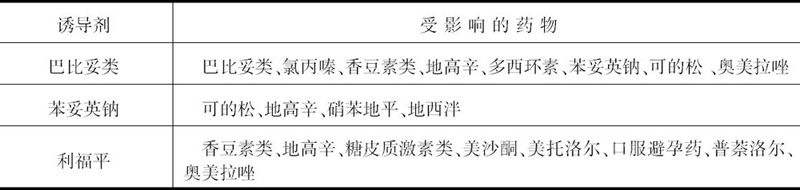
\includegraphics[width=5.89583in,height=2.59375in]{./images/Image00038.jpg}
\end{table}

区别咯血和呕血一般不难,但如患者出血急骤,量多或病史诉说不清时,有时鉴别并不容易;因此须详细询问有关病史,作细致的体格检查,及时作出诊断。

如已明确为咯血,须进一步探索其原因。引起咯血的原因很多(表\ref{tab4-2}),其中最常见的疾病是肺结核、支气管扩张、肺脓肿、支气管肺癌。此外支气管结石、肺寄生虫病、心血管疾病(特别是二尖瓣狭窄)、结缔组织病、钩端螺旋体病等也可引起咯血。

\begin{table}[htbp]
\centering
\caption{引起咯血的常见疾病分类}
\label{tab4-2}
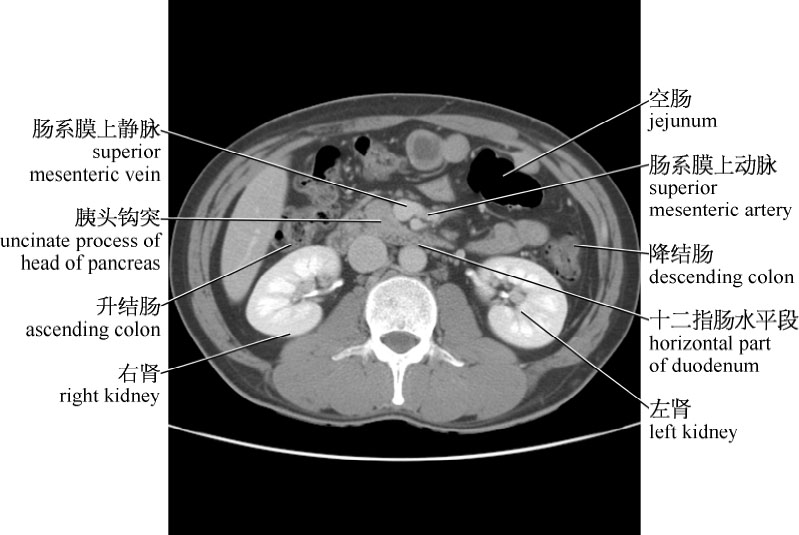
\includegraphics[width=5.89583in,height=4.80208in]{./images/Image00039.jpg}
\end{table}

如咯血量较大,应即采取急救措施,以尽早确定出血的部位。当X线检查的条件未具备时,可应用听诊法以确定。如咯血开始时一侧肺部呼吸音减弱或(及)出现湿啰音,而对侧肺野呼吸音良好,常提示出血即在该侧。气管和支气管疾病所致出血,全身症状一般不严重,胸部X线检查基本正常,或仅有肺纹理增粗;肺部病变所致出血,有比较明显的全身症状,胸部X线检查常发现病变阴影;必须指出,咯血可为全身疾病表现的一部分,临床医生必须对咯血患者做全身检查,以作出正确的诊断。

对于咯血患者,全面分析病史资料常可对咯血原因做出初步估计,同时还需要进一步做下列有关检查:

\subsection{1.病史}

须询问出血为初次或多次。如为多次,与以往有无不同。发生于幼年可见于先天性心脏病;儿童少年慢性咳嗽伴小量咯血和低色素性贫血,须注意特发性肺含铁血黄素沉着症;青壮年咯血多注意肺结核、支气管扩张等疾病;40岁以上有长期大量吸烟史(纸烟20支/
日×20年以上)者,要高度警惕支气管肺癌的可能性;年轻女性反复咯血也要考虑支气管结核和支气管腺瘤。在既往史上需注意幼年是否曾患麻疹、百日咳。在个人史中须注意结核病接触史、多年吸烟史、职业性粉尘接触史、生食螃蟹与蝲蛄史、月经史等。

细致观察咯血的量、颜色,有无带痰。肺结核、支气管扩张、肺脓肿、支气管结核、出血性疾病咯血颜色鲜红;肺炎球菌大叶性肺炎、肺卫氏并殖吸虫病和肺泡出血可见铁锈色血痰;烂桃样血痰为肺卫氏并殖吸虫病最典型的特征;肺阿米巴病可见脓血样痰呈棕褐色,带腥臭味;砖红色胶冻样血痰主要见于克雷伯杆菌肺炎;二尖瓣狭窄肺淤血咯血一般为暗红色;左心衰竭肺水肿时咳浆液性粉红色泡沫样血痰;并发肺梗塞时常咳黏稠暗红色血痰。大量咯血常由于空洞型肺结核、支气管扩张、慢性肺脓肿、动脉瘤破裂等所致;国内文献报告,无黄疸型钩端螺旋体病也有引起致命的大咯血。而痰中带血持续数周或数月应警惕支气管肺癌;慢性支气管炎咳嗽剧烈时可偶有血性痰。

详细询问伴随症状如发热、胸痛、咳嗽、痰量等。咯血伴有急性发热、胸痛常为肺部炎症或急性传染病,如肺出血性钩端螺旋体病、流行性出血热;咯血、发热同时伴咳嗽、咳大量脓痰多见于肺脓肿;长期低热、盗汗、消瘦的咯血应考虑肺结核;反复咳嗽、咳脓痰不伴有发热多见于支气管扩张。

\subsection{2.体格检查}

活动期肺结核和肺癌患者常有明显的体重减轻,而支气管扩张患者虽反复咯血而全身情况往往较好。有些慢性心、肺疾病可伴有杵状指(趾)。锁骨上淋巴结肿大在中老年患者要注意肺内肿瘤的转移。肺部闻及局限性哮鸣音提示支气管有狭窄、阻塞现象,常由肿瘤引起。肺部湿性啰音可能是肺部炎症的体征,也应考虑是否为血液存积在呼吸道所致。对咯血患者还应注意有无全身的出血表现。

\subsection{3.实验室检查}

痰检查有助于发现结核杆菌、真菌、癌细胞、肺吸虫卵等。出血时间、凝血时间、凝血酶原时间、血小板计数等检查,有助于出血性疾病的诊断。外周血红细胞计数与血红蛋白测定可推断出血的程度。外周血中嗜酸性粒细胞增多提示寄生虫病的可能性。

\subsection{4.X线检查}

对于咯血患者,除个别紧急情况不宜搬动外,均应做胸部X线检查。肺实质病变一般都能在X线胸片上显示阴影,从而及时作出诊断。如疑有空洞、肿块,或见肺门、纵隔淋巴结肿大,可加做胸部X线体层摄片或CT检查,CT还有助于发现细小的出血病灶。对疑有支气管扩张者,可做高分辨CT检查等协助诊断。对疑为支气管动脉性出血所致大咯血,必要时可行CT支气管动脉造影(CTA)或数字减影血管成像(DSA)检查,明确出血部位,后者尚可同时进行栓塞介入治疗。

\subsection{5.纤维支气管镜检查}

原因未明的咯血,尤其伴有支气管阻塞者,应考虑纤维支气管镜检查,可发现气管和支气管黏膜的非特异性溃疡、黏膜下层静脉曲张、结核病灶、肿瘤等病变,并可在直视下钳取标本作病理组织检查,吸取分泌物或灌洗液送细菌学和细胞学检查。

\subsection{6.其他检查}

先天性心脏病的诊断往往借助右心导管检查。放射性核素67镓对恶性肿瘤组织较健康组织有更大的亲和力,因而枸橼酸67镓肺部扫描可能有助于肺癌与其他肺部肿物的鉴别诊断。PET/CT对肺部肿瘤引起的咯血的诊断也有帮助。

咯血量的多少视病因和病变性质而不同,但与病变的严重程度并不完全一致,少则痰中带血,多则大口涌出,一次可达数百或上千毫升。临床上常根据患者咯血量的多少,将其分为少量咯血、中量咯血和大量咯血。但界定这三种情况的咯血量多少的标准尚无明确的规定,但一般认为24小时内咯血量少于100ml者为小量咯血;100~500ml/d者为中量咯血;>500ml或一次咯血量>100ml者为大量咯血。

临床上无异常肺部X线征象的咯血病例并不少见,诊断较为困难,其主要原因可能为:①气管或大支气管的非特异性溃疡,一般表现为小量咯血或血痰,支气管镜检查可以发现。②气管或支气管的静脉曲张,多见于右上叶支气管开口处或隆突部分,常引起大咯血,无痰,可经支气管镜检查而发现。③肺动脉瘤、支气管小动脉粥样硬化破裂,肺动静脉瘘破裂。④小块肺栓塞,常不易发现,一般有心脏病、下肢深静脉血栓形成、外伤史、长时间卧床或处于产褥期病史。⑤钩虫蚴、蛔虫蚴、血吸虫毛蚴、比翼线虫在肺内游移引起咯血。⑥早期支气管肿瘤,轻度支气管扩张、支气管结核,肺结核早期等。纤维支气管镜的广泛应用,结合胸部X线检查大大提高咯血病因的确诊率,国内一组917例经胸部X线与纤维支气管镜检查而确定的咯血病因如表\ref{tab4-3}所示:\footnote{*既有临床表现又有X线表现}

\begin{table}[htbp]
\centering
\caption{917例咯血的病因分析(X线诊断与纤支镜诊断比较)}
\label{tab4-3}
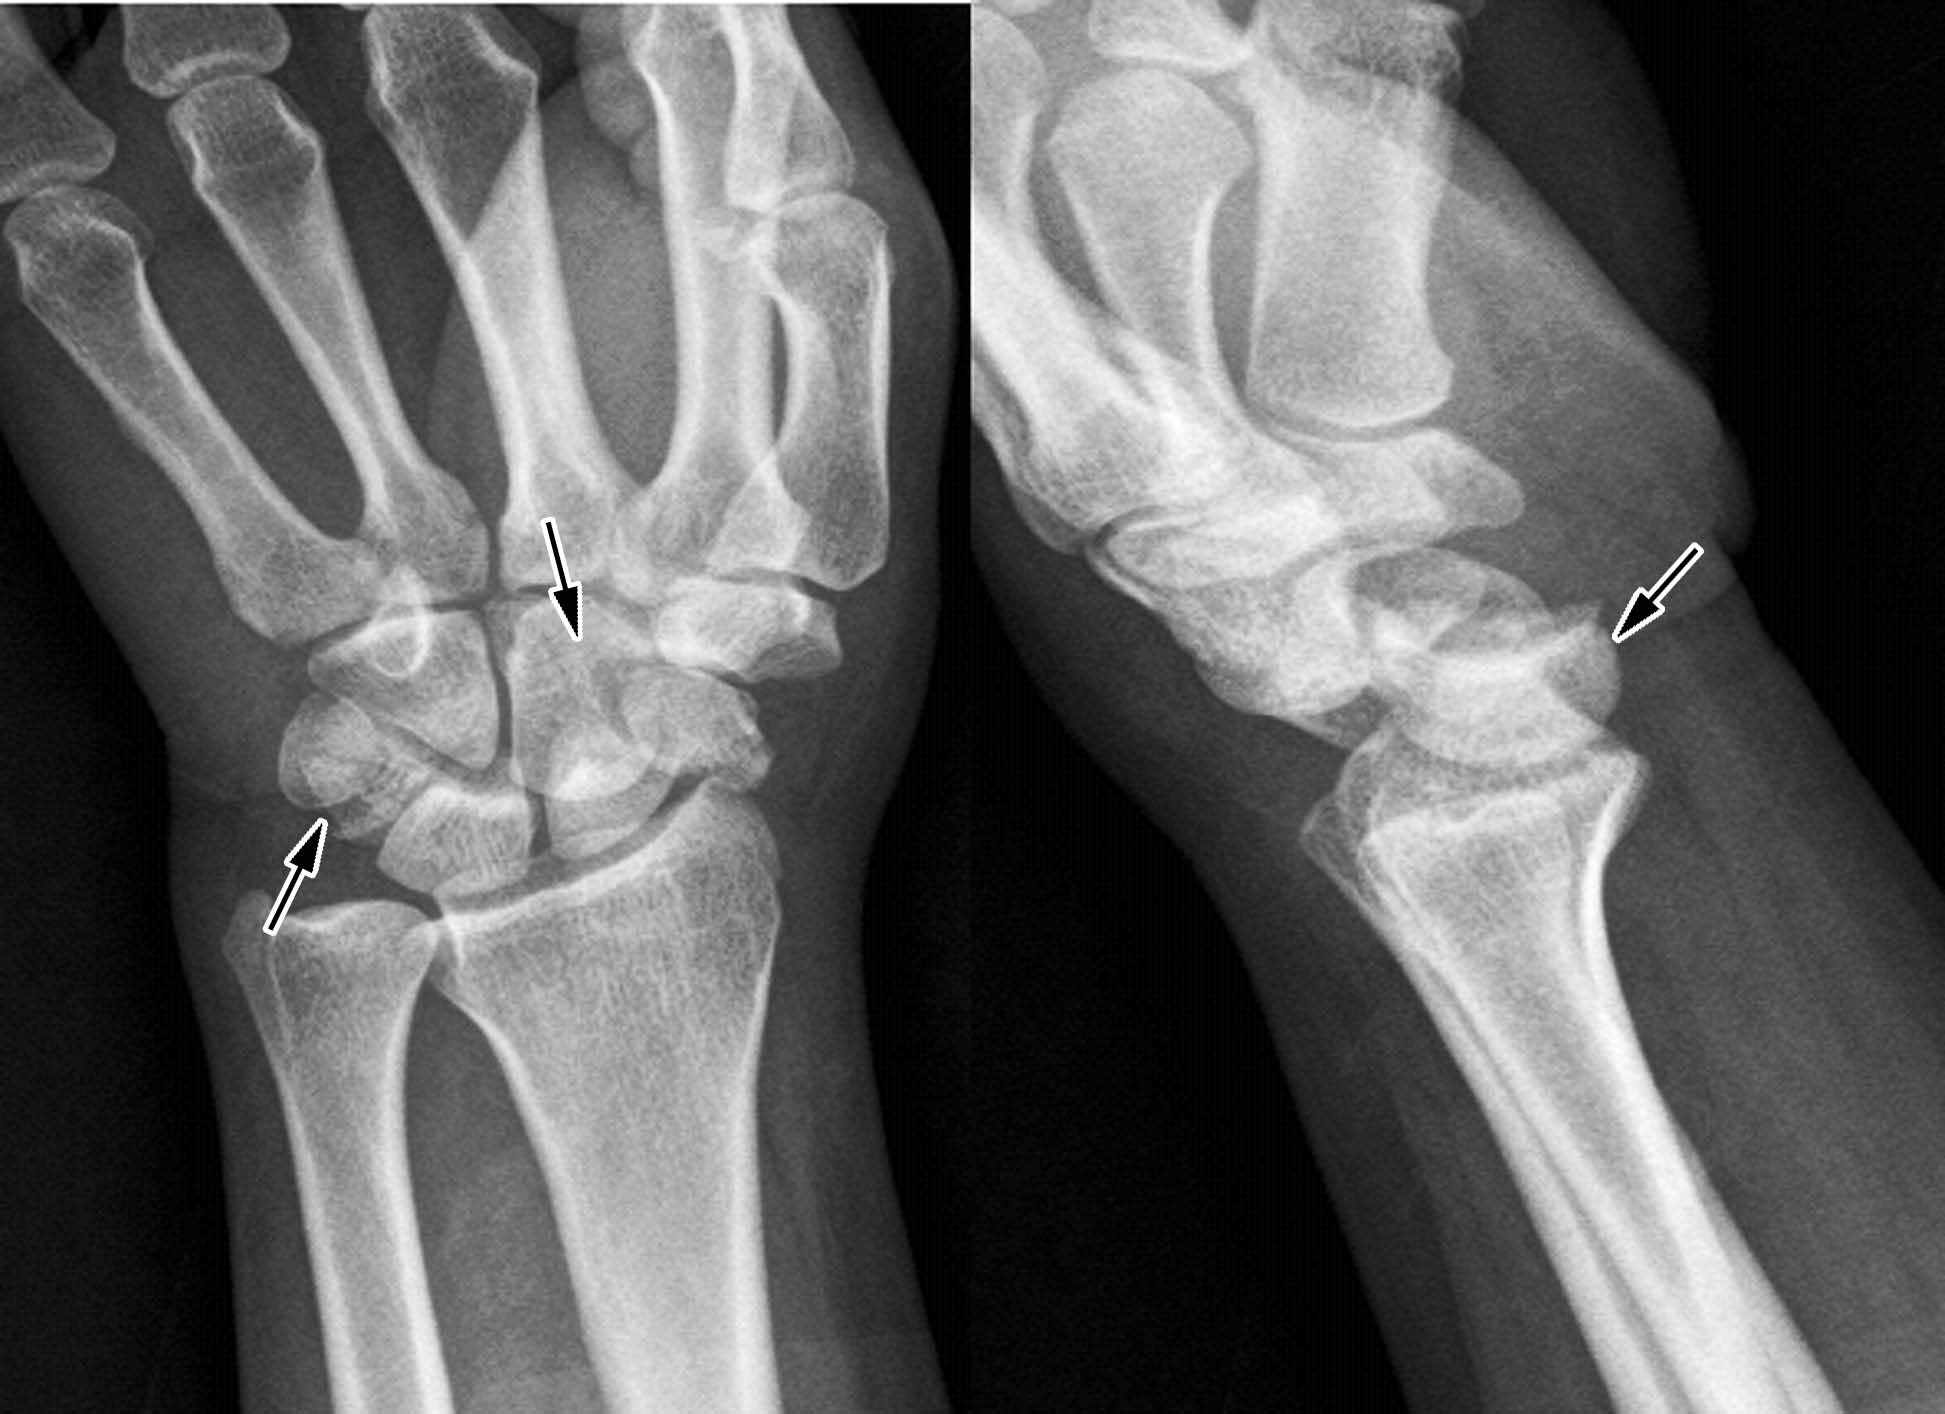
\includegraphics[width=5.91667in,height=3.58333in]{./images/Image00040.jpg}
\end{table}

由表\ref{tab4-3}所示,有部分咯血患者虽经X线和纤维支气管镜检查,仍未能发现阳性结果,且患者亦无引起咯血的全身性疾病,此类咯血可称为特发性咯血。但仍有可能在以后随诊中,在这类“特发性咯血”患者的一部分中,检出呼吸系统疾病。

国内曾有报告一组390例胸片无明显异常的咯血患者,作纤维支气管镜检查,结果发现肺癌16例(4.1\%)、支气管结核2例、支气管腺瘤1例,支气管囊性静脉曲张出血l例。作者认为咯血患者40岁以上,吸烟指数(吸烟年限×每天吸烟支数)>400,咯血时间长,且为痰血而非纯咯血者,尤须警惕肺癌的可能性。

X线胸片是咯血患者的常规检查,但可能无阳性发现。X线胸片正常的咯血患者应进一步作病因学诊断。有作者推荐应先作CT检查,以期发现潜在的肺部病灶,并有助于以后做纤维支气管镜检查时,有目标地进行刷检、活检取材,提高咯血的病因学诊断率。

\protect\hypertarget{text00057.html}{}{}

\subsection{12.1 气管和支气管疾病}

\subsubsection{一、急、慢性支气管炎}

急、慢性支气管炎患者有时也可咯血,一般为小量或痰中带血,不需治疗,可在数天内自行停止,但易于再发。如出血量大,需注意其他原因。本病的咯血与支气管炎症加剧有一定的关系,故咯血前常有病情加重的表现。慢性支气管炎患者发生持续的小量咯血时,须小心寻找其他原因,特别是支气管肺癌。

\subsubsection{二、非结核性支气管扩张}

非结核性支气管扩张可分为原发性与继发性。继发性者是由于支气管内或支气管外阻塞,引起支气管腔与支气管壁的感染,从而损害支气管壁的各层组织所引起。原发性支气管扩张则无明显的引起支气管阻塞的因素,但多数有肺炎病史,特别是麻疹、百日咳、流感等所继发的支气管肺炎史。

咯血是非结核性支气管扩张的常见症状,文献报告约90\%患者有不同程度的咯血,并作为提示诊断的线索。咯血可从童年即开始,常伴有杵状指(趾)。

此病的咯血有两种不同表现:

\paragraph{1.小量咯血}

在经常有慢性咳嗽、脓痰较多情况下,同时有小量咯血;有时在咯血前先有咳嗽较剧烈的一段感染加重阶段。因感染导致支气管内肉芽组织充血及损伤小血管而出现咯血。

\paragraph{2.大咯血}

由于支气管有炎症病变,血管弹性纤维被破坏,管壁厚薄不匀或形成假血管瘤,加上炎症影响,易破裂引起大咯血。咯血量每次达300~500ml以上,色鲜红,常骤然止血(因此类出血常来自支气管动脉系统,压力高,而动脉血管壁弹性好,收缩力强,故可较快止血)。

患者病程虽长,但全身情况尚好。咳嗽和咳痰也为常有的症状,咳嗽可轻微,也可相当剧烈;咳嗽和咳痰常与体位改变有关,如在晨起或卧床后咳嗽可加剧,咳痰增多。痰量可为大量,每天达数百毫升(湿性型)。痰液静置后可分为三层:上层为泡沫状黏液,中层为较清的浆液,下层为脓液及细胞碎屑沉渣。有些患者痰量甚少(干性型),如合并感染,痰量随之增多,并有发热、咯血等。

支气管扩张的好发部位是下肺,以左下叶较右下叶为多见,最多累及下叶基底段,病灶可延伸至肺边缘。病变部位出现呼吸音减弱和湿性啰音,位置相当固定,体征所在的范围常能提示病变范围的大小。

胸部X线平片检查不易确诊本病。国内一组84例非结核性支气管扩张中,只1/3病例在胸部X线平片上有少许的征象,大部分甚至没有任何改变。胸部X线平片检查对排除慢性肺脓肿及慢性纤维空洞型肺结核颇有帮助。如患者有支气管扩张的临床表现,X线胸片又显示一侧或双侧下肺纹理增粗、紊乱以及蜂窝状小透亮区,或见有液平面则支气管扩张的可能性最大,胸部CT检查可确定诊断,并对明确病变部位及决定治疗方案有重要意义。

全内脏转位、支气管扩张、鼻窦病变三联症,又称Kartagener综合征,国内有少数病例报告。此综合征有咳嗽、咳痰、咯血等症状。咯血可从童年开始,反复发作,量不多。

\subsubsection{三、结核性支气管扩张}

结核性支气管扩张的症状因肺内结核病灶的情况而定,如肺结核病灶不严重,则可无明显症状。有时或可闻及少许干、湿性啰音。X线胸片上显示病灶似已硬结,而患者仍有或多或少的咯血,应考虑结核性支气管扩张的可能性。国内一组64例患者中,发病大多在30岁以上,90\%有咯血(痰中带血或大量咯血)。病灶部位大都在两肺上叶,尤以右上叶的后段、左上叶的尖后段多见。

结核性支气管扩张与非结核性支气管扩张的鉴别见表\ref{tab4-4}。

\subsubsection{四、支气管结核}

支气管结核一般为继发性,原发性者罕见。患者大多有咯血,其他常见症状为阵发性剧烈咳嗽、喘鸣、阵发性呼吸困难等。有时轻度动作即可引起呼吸困难与发绀。如发生支气管阻塞,则引起突然的发热、痰量减少,而阻塞解除后痰量突然增加,体温也下降。

\begin{table}[htbp]
\centering
\caption{结核性与非结核性支气管扩张的鉴别要点}
\label{tab4-4}
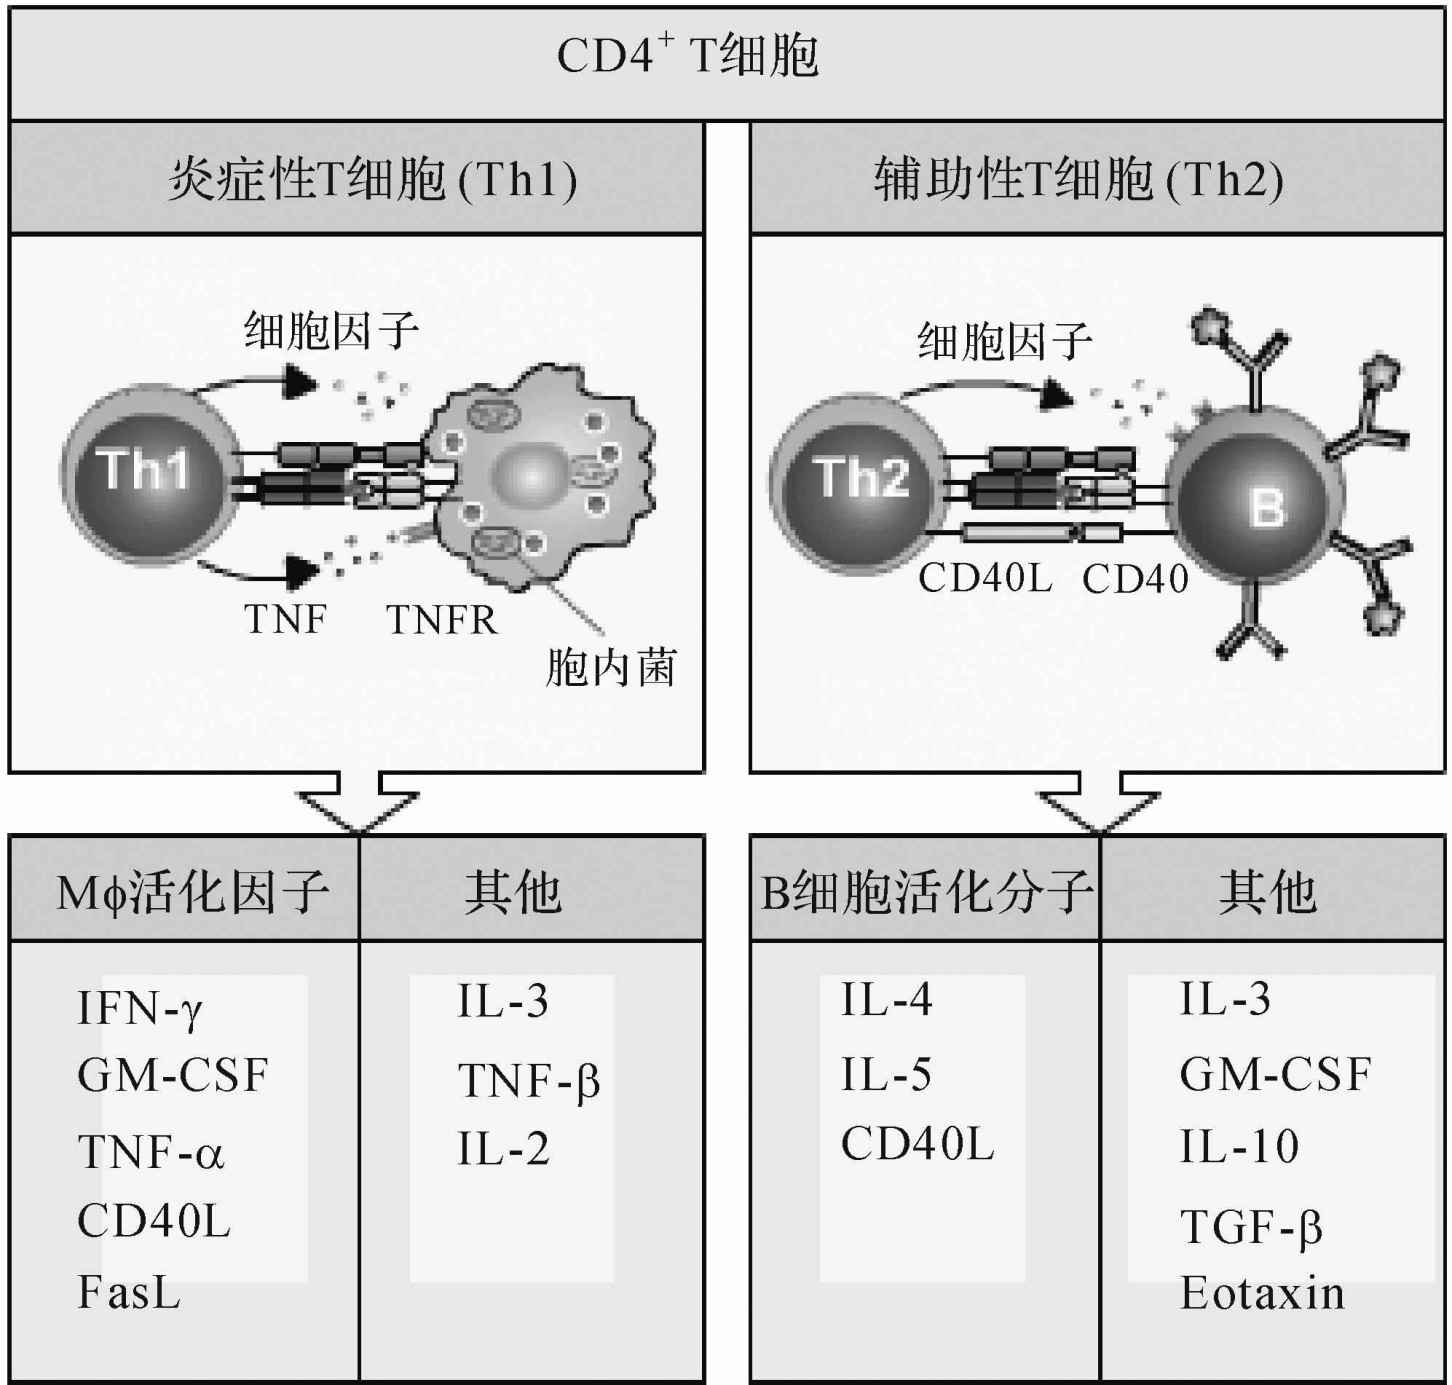
\includegraphics[width=5.94792in,height=1.65625in]{./images/Image00041.jpg}
\end{table}

支气管结核是发生于气管、支气管黏膜或黏膜下层的结核病变。据国内报告,肺结核合并支气管结核者占23.6\%~57.1\%。患者以青壮年为多,文献报告女性罹患多于男性,常发生于慢性纤维空洞型肺结核、慢性血行播散型肺结核、支气管淋巴结结核、浸润型肺结核及干酪样肺炎等基础之上。这些患者有下列情况提示有支气管结核的可能:①反复小量咯血或血痰而X线胸片未见明显病变者;②药物难以控制的刺激性咳嗽;③有喘鸣音;④有不同程度的呼吸困难而不能用肺实质病变解释者;⑤肺无明显病变而痰结核菌屡为阳性;⑥肺内有新播散病灶而不能用其他原因解释;⑦肺结核并发肺不张;⑧某些肺野空洞:在萎陷疗法后产生的张力性空洞;空洞时大时小;出现圆形、薄壁空洞;肺门附近的空洞等。

支气管结核的确诊须依靠纤维支气管镜检查。如临床症状典型,虽纤维支气管镜检查阴性,也不能除外此病的存在。

近年国内一组单纯气管、支气管结核病28例报道,误诊颇多,原因为:①胸片无异常发现;②胸片虽出现局限性肺气肿、肺纹理密集、肺纹理粗乱、叶间胸膜影移位等异常表现,但又非特异性而未加注意。作者建议对干咳、胸闷、喘息、咳黏液痰或咯血患者,经抗感染及对症治疗2周未见好转时.应及早作纤维支气管镜检查,镜下刷检涂片染色找抗酸杆菌,或钳取组织做病理检查。镜下所见仍疑似结核而实验室检查阴性时,2周后应再做纤维支气管镜检查。

目前将刷检标本或支气管肺泡灌洗液进行PCR检测结核分枝杆菌,可大大提高病原学诊断率。

结核感染T细胞斑点(T-SPOT.TB)试验是近年来的一项新诊断技术,通过检测外周血分泌γ-干扰素的T淋巴细胞数量来诊断结核感染,具有较高的特异性和敏感性,且不受卡介苗接种和环境分枝杆菌感染的影响,在肺结核的筛查和诊断中有较好的应用价值。

\subsubsection{五、支气管结石}

本病的特点为反复咯血,而肺部除有钙盐沉积之外,无其他原因可解释。患者或曾有咳出结石史。咯血通常为小量,但有些患者可有大咯血。X线检查发现有支气管结石阴影,以右中叶根部较为多见,结石远端可发现有阻塞性肺不张或肺部感染,CT检查可见支气管阻塞远端有钙化影。纤维支气管镜检查可帮助诊断。支气管结石常由肺结核病灶钙化引起。X线胸片上如炎症病变相应部位有钙化结节,在炎症消退后而咯血不断者,则支气管结石的可能性甚大。

据国内一组20例的报告中,以咯血为主要症状者占95\%,其中威胁生命的大咯血占40\%。误诊率60\%。并发症(占85\%)表现为肺不张、支气管扩张、阻塞性肺炎等。但手术治疗效果好。X线断层摄片、胸部CT和纤维支气管镜检查等综合检查对诊断有较大帮助。

\subsubsection{六、原发性支气管肺癌(肺癌)}

本病大多见于40岁以上男性,文献报告有咯血者占50\%~70\%,国内一组141例报告中,第一个月内出现咯血者有38.3\%。中央型肺癌较周围型肺癌易引起咯血。癌组织内小血管较多,患者又常有刺激性咳嗽,易引起癌组织损伤而致出血。其特点是痰中带血或小量咯血多见,而大量咯血少见,但晚期可有致命性大咯血。咳嗽是较常见的早期症状,无痰或有少量的白色黏液痰,可伴有胸痛。间断的或持续的小量咯血,对提示此病的诊断有重要意义。痰中可混有小颗粒状灰白色坏死组织,其中较易找到癌细胞。X线胸片、纤维支气管镜、胸部CT及活组织病理检查有助于诊断。

国内一组确诊肺癌患者1105例中,纤维支气管镜下直接见到肿瘤病灶(直接征象)者638例(57.7\%),只见肿瘤间接征象,即支气管黏膜改变者412例(37.3\%)。肺癌多见于段以上的支气管(中央型肺癌约占3/4),有些病例第一次活检及刷检均未能确诊,需做第二次,偶尔还要第3~4次检查。当发现有间接征象的可疑病例,应尽可能多部位活检多取标本,甚至看到癌体也应多点活检。

\subsubsection{七、支气管类癌}

支气管类癌罹患多为中年人,男女性别无差异,生长慢,具有恶性程度低和较少发生转移的特点。早期症状常为咯血,术后长期生存率较高。国内一组17例报告中,患者40岁以下者占64.7\%,中央型12例,周围型5例,2例有支气管旁淋巴结转移,主要临床表现为咳嗽、咳痰、咯血或痰中带血、发热和反复发作肺部炎症。临床上本病易误诊为肺癌、结核球或良性支气管肿瘤。X线检查与纤维支气管镜下活检对诊断帮助较大。

\subsubsection{八、良性支气管瘤}

良性支气管瘤少见,发病多在30~40岁之间。全身情况良好的中年患者如有反复的小量咯血或痰中带血,或类似哮喘发作,或屡次发作的呼吸道阻塞及感染症状,应考虑此病的可能。由于肿瘤生长缓慢,临床症状可延续多年。早期可无症状,或仅有气喘、干咳,有时甚至被误诊为支气管哮喘。肿瘤逐渐增大而堵塞支气管时,可发生相应肺叶的肺不张,并在肿瘤的远侧发生感染与支气管扩张。X线体层摄片、胸部CT,可了解较大的支气管内肿瘤的范围及部位,气道阻塞情况及继发性支气管扩张,对诊断有重要帮助。由于良性瘤多发生于较大的支气管内,纤维支气管镜检查的检出率可达85\%~90\%。

良性支气管瘤有腺瘤、平滑肌瘤、乳头状瘤等,此外较罕见的有纤维瘤、软骨瘤、脂肪瘤等。其中腺瘤比较多见,典型X线征象为肺门附近有圆形或类圆形阴影,密度均匀一致,边缘锐利,体层摄片或胸部CT检查更易于发现;由于多数腺瘤位于主支气管或肺叶支气管内,纤维支气管镜检查易作出诊断。

\protect\hypertarget{text00058.html}{}{}

\subsection{12.2 肺部疾病}

\subsubsection{一、肺结核}

咯血是肺结核患者常见的症状,且常为提示此病诊断的线索。咯血量多寡不一,少可仅为痰中带血,多则一次可达500ml以上,血色鲜红。咯血与结核病变的类型有一定关系,多见于浸润型肺结核、慢性纤维空洞型肺结核、干酪样肺炎,而少见于原发综合征(原发型肺结核)和急性血行播散型肺结核。咯血严重程度并不一定与病灶大小成正比,小的病灶可有较多的咯血,而病灶广泛的也可无咯血。出血量常和血管损害程度有关,血管壁渗透性增高所致的咯血,出血量少,但持续时间较长;小血管的破裂则多引起小量出血,这往往由于慢性活动性肺结核所致;大咯血多为肺动脉分支破损所致,其中以空洞内形成的动脉瘤破裂所致的大咯血多见,此类出血来势甚急,而由于洞壁纤维化不易收缩止血,或血凝块虽能填塞空洞压迫血管暂时止血,但又可因血块溶解而再次出血。

肺结核患者以青壮年占大多数,不少患者以咯血为初发症状而就诊。咯血之后常有发热,是由于病灶播散及病情发展所致。患者常同时出现疲乏、纳差、体重减轻、午后潮热、盗汗、脉快和心悸等全身中毒症状。

肺结核的诊断主要依靠症状、体征、X线胸片和痰结核菌检查。如在青壮年人一侧肺尖部经常听到湿性啰音,又有上述全身性中毒症状,则支持活动性肺结核的诊断。X线胸片是诊断肺结核的重要方法,可以发现早期轻微的结核病变,确定病灶的范围、部位、形态、密度、与周围组织的关系,判断病变的性质、有无活动性、有无空洞、空洞大小和洞壁特点等。因此,定期进行胸部X线检查能及早发现病灶,有助于早期治疗。

痰结核菌检查阳性可确诊为肺结核,且可肯定病灶为活动性。但痰结核菌阴性并不能否定肺结核的存在,对可疑病例需反复多次痰液涂片检查,如有需要,可采用浓集法、培养法、PCR法等,在咯血前后,因常有干酪性坏死物脱落,此时的痰菌阳性率较高。

长期被误诊为肺结核咯血的肺部疾病并非少见,文献报道有支气管扩张、支气管囊肿、肺癌、肺脓肿、肺吸虫病等。

年轻患者反复咯血,痰结核菌检查阴性,全身情况较好,而病灶又处于中、下肺野,用一般抗菌药物治疗能改善炎症表现者,则可认为是非结核性支气管扩张,胸部CT检查有助于确定诊断。支气管囊肿在胸部平片及透视下一般可确定诊断。非结核性支气管扩张或支气管囊肿合并普通细菌感染时,其症状的出现通常较早,可追溯到童年时期,特别是在患麻疹、百日咳之后常有咯血及呼吸道炎症症状,其与肺结核病的鉴别是前两者在长期的病患过程中,全身一般状况仍较好,无结核病的全身中毒症状,可伴有杵状指(趾),痰结核菌阴性。

肺癌被误诊为肺结核者颇为常见。在下列情况下,应考虑肺癌的可能:①年龄在40岁以上,尤其是长期重度吸烟的男性患者,新近出现反复的咯血或持续的痰中带血,或近肺门处有致密的异常阴影,或出现肺不张合并感染,而多次痰液检查未发现结核菌者,应首先考虑肺癌的可能;但痰中结核菌阳性也不能除外肺结核与肺癌并存。②肺癌组织内部发生坏死破溃,坏死组织排出后形成空洞,其X线征象可酷似结核性空洞。但癌性空洞常呈偏心性,其内侧壁凹凸不平,外缘多呈毛刺状、分叶状,常无病灶周围卫星灶,多次痰结核菌检查阴性,经规律的抗结核治疗无效,病灶逐渐增大,这些均可与肺结核鉴别。③肺癌和肺结核并存,肺癌可发生在陈旧性肺结核瘢痕的基础上,而肺癌又能促使结核病灶恶化。如在陈旧性或活动性结核病灶处出现新的、致密的圆形病灶,且经积极抗结核治疗一个月后,病灶仍逐渐增大,或出现肺不张、肺门阴影增大,癌性空洞等改变,应考虑并存肺癌的可能。

\subsubsection{二、肺 炎}

在急性肺炎时,肺实质处于高度充血状态,小血管通透性增加并可发生破裂而致咯血。由于小血管可发生血栓性脉管炎,致血管腔闭塞,通常不易引起大量咯血。

肺炎链球菌肺炎的患者,痰中混有血液者并不少见,有时血量可达20~30ml,病期第2、3天转为铁锈色痰。在整个病程中均呈血性痰的甚少。

肺炎杆菌性肺炎多为砖红色稠胶样痰;化脓性链球菌肺炎咳粉红色稀痰;葡萄球菌肺炎可为血性痰、脓性痰;绿脓杆菌肺炎咯血少见,典型者咳翠绿色脓痰。军团菌肺炎少量黏液痰中可带血丝,并有发热、咳嗽、肌痛、关节痛、腹泻、蛋白尿、转氨酶升高、直接荧光抗体阳性或间接荧光抗体1∶256。肺炎支原体肺炎约1/4病例有血性痰,但绝无铁锈色痰;流感病毒性肺炎常引起反复的小量咯血。

\subsubsection{三、肺脓肿}

肺脓肿多由于吸入感染或血源性感染所引起,约50\%患者伴有咯血,常伴有大量脓痰或脓血样痰。急性肺脓肿的早期可有大量的咯血而无脓痰,但此时有寒战、高热、胸痛、血白细胞和中性粒细胞增高,提示急性细菌性感染,1周后可出现大量脓性痰。慢性肺脓肿常有大量的脓痰或脓血痰,痰量每天可达300~500ml,带臭味,痰静置分层,多数患者伴有杵状指。慢性肺脓肿常被误诊为肺结核病,前者可根据急性发病史、X线胸片见大片浓密模糊浸润阴影,脓腔内出现圆形透亮区及气液平面,痰培养可有致病菌生长以及抗菌治疗有效,一般鉴别不难。慢性肺脓肿与肺癌的区别,可根据肺脓肿过去的急性发病史、空洞的特点及痰中癌细胞检查等加以鉴别,X线胸片、纤维支气管镜、胸部CT扫描有利于诊断。癌性空洞与肺脓肿空洞、结核性空洞的鉴别参见表\ref{tab4-5}。

\begin{table}[htbp]
\centering
\caption{癌性空洞与肺脓肿空洞、结核性空洞的鉴别}
\label{tab4-5}
\includegraphics[width=5.97917in,height=3.53125in]{./images/Image00042.jpg}
\end{table}

\subsubsection{四、肺部真菌感染}

肺部真菌感染是最常见的深部真菌病,主要由念珠菌、曲霉、毛霉、新型隐球菌等真菌感染所致。老年、幼儿及体弱者易患此病,多为痰中带血或小量咯血。常见症状有发热、乏力、盗汗、纳差、消瘦、咳嗽、胸痛;痰的特点是量少,不同种类的真菌感染时,其痰的性状不一。肺白念珠菌感染,为胶样黏稠痰,带乳块或血丝;肺曲霉病反复咯血或咳出大量泡沫痰(可带酒味);肺新型隐球菌病则咳小量黏液性痰或血丝痰。病原学检查可找到致病菌,胸部X线检查,肺组织病理检查有助于诊断。

\subsubsection{五、肺寄生虫病}

\paragraph{1.肺阿米巴病}

阿米巴性肺脓肿为肝阿米巴病并发症之一,也可来自肠道病灶。多数起病较慢,常有发热、乏力、消瘦、咳嗽、咳痰、右下胸痛并放射至右肩,少数呈急性发病,高热、胸痛、呼吸困难等,可有肝脏肿大体征。典型的痰液呈棕褐色而带腥臭味,有助于此病的诊断。如合并出血或混合感染,可呈血性或黏液脓血痰。痰液、胸腔积液或纤维支气管镜取病变坏死组织中查找到溶组织阿米巴滋养体可确诊。

\paragraph{2.肺吸虫病}

本病有严格的地区性,患者都曾有在疫区进食未煮熟的含有肺吸虫囊蚴的石蟹或蝲蛄史。病程中常反复的小量咯血,痰血混合多呈特殊的棕黄色或铁锈色,烂桃样血痰是肺吸虫病最典型特征。早期症状有畏寒、发热、脐周隐痛、腹泻,并有乏力、盗汗、纳差,2~3周后出现咳嗽、胸痛、咯血等,患者虽有长期的反复咯血,但全身情况尚好,胸部体征多不明显,可有皮下结节。常有血嗜酸性粒细胞增多,痰中发现肺吸虫卵即能确诊,阳性率90\%以上。粪便虫卵检查、肺组织病理检查、免疫学检查、X线检查等有助于诊断。

胸部X线检查有较特别的征象,病灶多位于中、下肺野及内侧带,因病变的不同时期而有下列的表现:①早期呈边缘模糊的弥漫阴影,大小约为1~2cm;②中间期为边缘清楚、多房或单房的、实质或囊状的大小不等的阴影,多房性囊状阴影是本病的X线特征;③晚期为纤维增殖性变及硬结钙化阴影。此外,可有肺门增大、肺纹理增粗紊乱、胸腔积液或胸膜增厚等征象。对一些疑难的、不典型的病例,流行病学调查和免疫学检查,在诊断上有重要意义。

如患者有上述的流行病学史和胸痛、咳铁锈色痰等症状,血嗜酸性粒细胞增多,痰中虽未发现肺吸虫卵,而肺吸虫抗原皮内试验阳性,并已除外血吸虫病、华支睾吸虫等感染时,则大致可作出肺吸虫病的临床诊断,并应进行特效药物(如吡喹酮)的诊断性治疗;如疗效显著,可进一步确立诊断。肺吸虫病主要须与肺结核相鉴别(表\ref{tab4-6})。

\begin{table}[htbp]
\centering
\caption{肺吸虫病与肺结核鉴别}
\label{tab4-6}
\includegraphics[width=5.94792in,height=4.91667in]{./images/Image00043.jpg}
\end{table}

在四川及福建发现的肺吸虫病,临床表现较特别,其症状轻,咯血量较小,痰中虫卵检出率较低,有游走性皮下结节者甚多(多分布于胸壁及上腹壁),血中嗜酸性粒细胞显著增多。

国内报道肺吸虫病误诊率较高。主要原因是由于肺吸虫病临床表现及X线胸片大多无特异性,且典型的游走性皮下结节,肺空泡、结节和隧道线条等X线表现又少见。一组报道34例肺吸虫病在入院前全部误诊为肺结核。

由于肺吸虫病免疫学诊断的敏感性和特异性高,且简便易行,在流行区内患者有生食石蟹或蝲蛄史,而反复出现咳嗽、咯血或痰中带血、发热等症状,应即作肺吸虫抗原皮内试验,上述一组误诊为肺结核的34例患者,肺吸虫抗原皮内试验全部为1∶2000以上阳性。应用混合单抗双抗体夹心ELISA法诊断疑难肺吸虫病,效果更佳。

\paragraph{3.肺包虫病}

肺包虫病是棘球绦虫的幼虫(棘球蚴)寄生于人体肺内所引起,主要流行于畜牧区,以青壮年农民和牧民为主,早期可无症状。当包囊肿大破裂时可出现咯血或痰中带血,并可咳出类似粉皮样的角皮膜;合并感染时则出现咳嗽、咳痰、胸部不适,或胸痛及劳力后气促等症状。可有肝脏或其他部位囊肿征象。囊肿破裂,囊液亦可阻塞气管而引起窒息。X线胸片或CT扫描有助于诊断,可显示包虫圆形或卵圆形,略呈分叶状阴影,边缘清晰,密度均匀,壁可钙化,阴影随呼吸而变形;包虫囊壁破裂,空气进入,则顶部呈现半月形透亮带。包虫抗原皮内试验及补体结合试验对本病有重要的诊断意义,阳性率可达90\%以上。此外,痰检查、B超检查、放射性核素扫描等对诊断也有帮助。

\subsubsection{六、恶性肿瘤的肺转移}

恶性肿瘤转移至肺部时,可引起咯血。较常发生肺部转移的恶性肿瘤有鼻咽癌、乳腺癌、食管癌、胃癌、肝癌、结肠直肠癌、前列腺癌、睾丸畸胎瘤、精原细胞瘤、绒毛膜上皮细胞癌、恶性葡萄胎及类癌等。以绒毛膜上皮细胞癌、睾丸畸胎瘤和恶性葡萄胎的肺转移的咯血发生率最高。对成年女性原因未明的咯血,患者阴道曾排出水泡样胎块,或兼有流产后持续的不规则阴道出血,应考虑恶性葡萄胎或绒毛膜上皮细胞癌的可能性,尿妊娠诊断试验有助于此病的诊断。

转移性肺恶性肿瘤常为多发,但也可为单发,后者较少见。X线胸片显示多发性肺转移肿瘤的形态多为圆形、卵圆形或粟粒状阴影,大小相仿,边缘不整,发展较快。转移性肺恶性肿瘤原发病灶的诊断有时不易,须设法寻找。

\subsubsection{七、肺梅毒}

本病极为少见,国内仅有二例感染报告,均有咯血。病程进展缓慢,往往有咳嗽、咯血、胸痛等症状,虽然X线胸片显示下肺野呈大片状实质模糊阴影,但全身情况良好。诊断须依据梅毒感染史、梅毒血清反应阳性与驱梅治疗的疗效。肺梅毒须与其他肺部疾病相鉴别,特别是肺结核病。

\subsubsection{八、肺囊肿}

肺囊肿可区分为先天性与后天性两类,以前者较为多见,后者是由肺部感染性疾病或寄生虫所引起。多发性先天性肺囊肿常伴有支气管扩张,多在儿童期出现症状,其临床表现与支气管扩张相似,患者往往因突然小量咯血或痰中带血而就诊,由于病变多位于中、上肺,引流较好,较少出现发热。X线胸片检查呈圆形透亮影,其壁菲薄而整齐;多发者大小不一,可分布于任何肺野,但以中、上肺野较多见。

多发性先天性肺囊肿需与支气管扩张鉴别。肺囊肿继发感染时可出现大片状模糊阴影,类似浸润性肺结核,但经抗生素治疗后感染较快消退,而有别于肺结核。肺囊肿合并感染时,其临床症状和X线胸片的改变与肺脓肿相似,需加以鉴别。

国内曾报告一组82例的成年患者中,52例(63.4\%)有咯血,多数在200ml以下,认为如有下列情况应考虑本病:①肺部阴影长期存在;②阴影在同一部位反复出现;③无播散灶;④阴影新旧程度一致;⑤肺门及纵隔淋巴结不大。患者虽反复咯血而无结核中毒症状。胸部CT检查有助于对本病的诊断。

近年肺囊肿有一组38例报告,发病常在青少年期,5例初发年龄在10岁以下。全部患者(38例)在院外均被误诊为肺结核。初发症状以咯血或痰中带血多见(21/38),咳嗽、咳痰、发热次之。6例无症状患者经体检而发现本病。21例有长期反复出现咯血或痰中带血史,最长者达20年。

肺囊肿的胸部X线表现常缺乏特征性。作者认为以下几点有利于肺囊肿的早期诊断:①发病年龄在30岁以下,特别是男性,有反复咯血或痰中带血、咳嗽、发热史。②动态观察X线胸片阴影的形态变化不大,无肿瘤的淋巴结、淋巴道远处转移的改变。③结核菌素试验阴性或经积极的抗结核治疗无效。④胸部X线显示其病变虽无固定部位但与支气管走向有关;虽经反复感染但病变部位固定不变;在非囊肿部位不出现新的病灶。⑤有条件时应作高分辨胸部CT检查加以鉴别。⑥经上述不能确诊时应考虑肺活检或外科手术探查。

\subsubsection{九、尘 肺}

包括硅沉着病和其他尘肺,是由于长期吸入某种粉尘所致的以肺实质弥漫性纤维病变为主的疾病。主要发生于从事粉尘作业的工人,可有慢性、顽固性咳嗽,咳泡沫状痰、咯血或痰中带血,气短和胸痛。早期症状不明显,常为干咳或带黏稠痰,晚期咳嗽加重,痰多,如合并肺结核或支气管扩张,可反复大咯血。晚期病情重,有发绀、杵状指、肺气肿、肺源性心脏病等表现。胸片可见中、下肺野呈网状、条索状或结节状阴影改变,肺门淋巴结肿大。其诊断主要依据为职业病史、临床表现、胸部X线征象及肺功能检查。

硅沉着病合并肺结核比无硅沉着病的发病率高4~5倍,其特点是肺结核的发生率和严重程度与硅沉着病的发展程度成正比,硅沉着病愈严重,其并发肺结核的可能性愈大,肺结核病的病变发展也愈迅速,病情愈严重。石棉肺合并肺结核比较少见,但合并肺癌者却较多。

\protect\hypertarget{text00059.html}{}{}

\subsection{12.3 肺血管及其他循环系统疾病}

\subsubsection{一、肺血栓栓塞症}

肺血栓栓塞症是肺栓塞的最常见类型,占肺栓塞中的绝大多数,多继发于右心或体循环深静脉系统的血栓形成,偶尔也见于肺动脉炎、感染性心内膜炎等病例中,是以各种栓子阻塞肺动脉系统为其发病原因的一组疾病或临床综合征。主要症状为呼吸困难及气促、胸痛、小量咯血(大咯血少见)、咳嗽、心悸、发热等。心瓣膜病(特别是合并心房颤动)患者发生咯血、未能解释的短期发热时,须考虑肺血栓栓塞症的可能。X线胸片可显示区域性肺纹理变细、稀疏或消失,肺野透亮度增加;也可显示肺组织的继发改变,如肺野局部的片状阴影,尖端指向肺门的楔形阴影,肺不张或膨胀不全,有肺不张侧可见横膈抬高。X线胸片对鉴别其他胸部疾病有重要帮助。螺旋CT、放射性核素肺通气/血流灌注扫描、磁共振显像(MRI)及肺动脉造影都是肺血栓栓塞症的重要确诊方法。

\subsubsection{二、肺动脉高压}

肺动脉高压可由许多心、肺和肺血管疾病引起,根据发病的原因是否明确,曾被习惯性分为“原发性”和“继发性”肺动脉高压。2008年世界卫生组织第4届肺动脉高压会议重新修订了肺动脉高压分类,目前按照病因或发病机制、病理与病理生理学特点分为五个大类:①动脉性肺动脉高压;②左心疾病所致肺动脉高压;③肺部疾病及(或)低氧所致肺动脉高压;④慢性血栓栓塞性肺动脉高压;⑤未明多因素机制所致肺动脉高压。继发性肺动脉高压较原发性肺动脉高压常见,早期临床表现以基础疾病如慢性支气管炎、COPD等的临床表现为主,晚期以右心功能不全的表现为主。原发性肺动脉高压是一少见病,被世界卫生组织改称为“特发性肺动脉高压”,是一种不明原因的肺动脉高压。早期通常无症状,仅在剧烈活动时感到不适;随着肺动脉压力的增高,可逐渐出现呼吸困难、胸痛、头晕或晕厥、咯血。咯血量通常较少,有时也可因大咯血而死亡。其他症状还包括疲乏、无力,雷诺现象,声嘶(Ortner综合征)等。胸部X线检查、超声心动图和多普勒超声检查、放射性核素肺通气/灌注扫描、右心导管术、肺活检都对诊断有重要的作用。

\subsubsection{三、肺动静脉瘘}

肺动静脉瘘是先天性肺血管的血管瘤样畸形,也可为获得性,临床上少见。可有咳嗽、间歇小量咯血、发绀、杵状指(趾)及红细胞增多症。体格检查可发现在相应胸壁部位触及震颤,闻及来回性血管杂音。X线胸片和胸部CT在诊断上起重要作用,可见边缘整齐、密度均匀的圆形或卵圆形阴影,多位于中下肺野,且与肺门之间有条索状阴影,病变无钙化,无空洞形成。肺动静脉瘘发病常与遗传性出血性毛细血管扩张症有关,可误诊为肺结核球或支气管肺癌,肺动脉造影可协助明确诊断。

\subsubsection{四、单侧肺动脉发育不全}

本病少见,患者大多有不同程度的咳嗽、咳痰、痰中带血、胸痛、气促等表现,体格检查可发现患侧胸廓扩张稍受限、语颤及呼吸音减弱、多可听到干、湿性啰音,可被误诊为肺气肿、气胸、支气管扩张等。诊断主要依靠胸部X线检查,尤其是胸部CT的肺动脉造影对诊断极有帮助。

\subsubsection{五、肺淤血}

常见于风湿性心脏病二尖瓣狭窄,且多发生在较严重的瓣口狭窄的慢性充血期,也可见于急性左心衰、复张后肺水肿、高原性肺水肿等,多表现为痰带血丝、小量咯血或咳出粉红色泡沫样痰。结合心脏病史、胸腔快速抽液(气)及快速登山等病史,心尖部舒张期隆隆样杂音,超声心动图和多普勒超声检查等可作出诊断。二尖瓣关闭不全较少引起咯血。

\subsubsection{六、高血压}

在恶性或急进型高血压,由于血压持续增高时,可引起肺毛细血管破裂而出现咯血。也可由于并发急性肺水肿而咳粉红色泡沫样痰。

\subsubsection{七、先天性心脏病}

某些有血液分流的先天性心血管病如房间隔缺损、室间隔缺损、艾森曼格综合征等,均可伴有显著的肺动脉高压,由此可引起咯血。

\protect\hypertarget{text00060.html}{}{}

\subsection{12.4 全身性疾病及其他原因}

\subsubsection{一、急性传染病}

1.肺出血型钩端螺旋体病
肺出血型钩端螺旋体病也称钩端螺旋体性出血性肺炎,是钩端螺旋体病的严重类型,如不注意常易误诊。钩端螺旋体病以夏秋季多发,以青壮年为主,从事牧、渔业劳动者发病率高,大多起病急骤,症状主要有畏寒或寒战、高热、头痛、全身肌肉酸痛、衰弱无力、眼结膜充血、腓肠肌疼痛、淋巴结肿大,多在毒血症过程中出现心悸、烦躁、呼吸和心律逐渐增快。初为痰中带血,以后咯血量增多。严重的肺弥漫性出血型者,可引起致命的大咯血,其特点是发生突然、发展迅猛,临终时多数患者出现从口鼻涌出大量血液,立即窒息而死。X线胸片和胸部CT显示双侧肺野斑片状模糊阴影,以中、下肺野尤其显著。需与其他原因的肺炎、肺结核鉴别。病原学和血清学检查有助于明确诊断。

2.流行性出血热
由汉坦病毒引起,经呼吸道、消化道、母婴、虫媒及动物源传播,流行季节以3~5月份或5~7月份以及11月份至次年1月份间为高峰,青壮年多见,主要损害全身小动脉和毛细血管。患者起病急,典型病例具有发热、出血与肾损害三大主要特征以及发热期、低血压休克期、少尿期、多尿期和恢复期五期经过。其主要临床表现为发热、头痛、腰痛、眼眶痛、口渴、呕吐、酒醉貌、球结膜充血水肿,皮肤和黏膜广泛出血、鼻出血、咯血、呕血、便血、血尿,软腭及腋下有出血点,肾区有叩击痛。早期外周血白细胞正常或偏低,有尿蛋白,尿红、白细胞及管型改变;肾功能损害,约有半数出现肝功能损害。特异性血清学试验有助于确诊。

\subsubsection{二、血液病}

某些血液病如血小板减少性紫癜、白血病、再生障碍性贫血、血友病等均可出现咯血,与原发病有关。除咯血外,尚伴有其他部位的出血倾向。血常规、骨髓细胞学检查、血小板功能与凝血因子检查可确诊。

\subsubsection{三、白塞病(Behcet disease)}

本病由病毒感染、遗传因素、免疫功能及体内微量元素异常等因素引起。初发年龄主要是16~40岁的青壮年,以女性多见。基本病变是血管炎,可累及毛细血管和细小动静脉,可因肺部血管受累而反复咯血,多为小量咯血,也有因肺脉管炎而引起多发性肺栓塞。主要的临床表现为反复发作的口腔黏膜、舌尖及其边缘、齿龈、上下唇内侧等处的痛性小溃疡;外生殖器损害与口腔基本相似;眼部损害主要为结膜炎、角膜炎、虹膜炎、视网膜炎,其他表现有皮肤损害、消化道损害、关节损害及神经系统损害等。活动期多有血沉、黏蛋白、唾液酸、α2球蛋白增高,部分患者血浆铜蓝蛋白及冷球蛋白阳性。本病并发肺脉管炎引起咯血时的胸部X线表现,可类似肺炎支原体肺炎、肺部转移癌,或出现大片密度增高的圆形阴影。病理学检查及有关脏器病变的相应检查有助于诊断。针刺反应阳性是一特征性表现,若能同时检查HLA-B5,对本病的诊断更有帮助。

\subsubsection{四、结缔组织病}

该类疾病如系统性红斑狼疮、结节性多动脉炎、重叠综合征等,其发病与遗传、某些药物、物理因素、病毒感染、内分泌因素、免疫异常等有关,多见于20~40岁的女性。可有小量咯血,如伴有肺动脉受侵害,可发生大咯血。若患者有多个器官系统功能的损害,胸部X线检查见肺部有阴影,而抗菌药物治疗效果不佳时,应考虑结缔组织病伴有肺部损害的可能性。诊断结缔组织病所致的咯血时,须认真除外肺结核、支气管扩张、肺肿瘤等疾病。实验室检查和肺组织病理检查有助于诊断。

\subsubsection{五、肺出血-肾炎综合征}

国外文献曾有多例重度肺出血合并肾小球性肾炎报告,并命名为Goodpasture综合征,病因未明,也有将此病归入结缔组织病,临床上少见。此病多见于20~40岁男性,病程数月至数年,预后不良。临床经过可分为两个阶段:①肺部病变阶段,87\%~96\%以上的病例的首发症状表现为间歇的咯血,轻者为血痰,重者出现大咯血,反复出血可致贫血;病变广泛者可有呼吸困难、发绀与胸痛,X线胸片上显示短暂的弥漫性细小或大片状阴影,但X线检查也可呈阴性。②肾脏病变阶段:多数患者在咯血后数周或数月出现肾炎症状,肾脏病变表现为肾小球性肾炎,起病隐袭,当肺部病变显著时,尿检查发现蛋白尿、镜下血尿与管型尿,早期肾功能正常,当肾脏病变为进行性,尿毒症症状迅速出现,并掩盖肺部症状。X线、痰涂片、尿常规、血液检查、免疫学检查、肺功能检查都有助于诊断。肾组织活检免疫荧光检查,发现抗肾小球基底膜抗体则可明确诊断。通常由于尿毒症导致死亡。

除肺、肾两脏器之外,其他脏器很少受累。高血压少见。

\subsubsection{六、肉芽肿性多血管炎(韦格纳肉芽肿)}

是一种原因未明的综合征,被认为是机体对未知抗原的异常超敏反应所致。以30~50岁男性多见,具有上下呼吸道坏死性肉芽肿性血管炎,肾小球肾炎和小血管炎的临床表现。常有小量咯血,严重者可发生大量肺泡性出血,患者可伴有发热、乏力、纳差、关节痛、肌痛;上呼吸道症状有鼻分泌物增多、口咽部溃疡、声嘶;肺部症状有咳嗽、胸痛、呼吸困难;肾损害表现有不同程度的蛋白尿、镜下血尿或红细胞管型;其他表现可有皮肤黏膜损害、血疱、结节、红斑、结膜角膜炎、多发性神经炎、心肌炎、耳部损害。胸部X线检查表现为肺单侧或双侧多发或孤立结节影,大小不等,边界清楚,多有空洞形成,空洞壁薄而形态不规则,罕有液平存在。口咽、肺、肾组织活检及实验室检查有助于诊断,典型病例胞浆型抗中性粒细胞胞浆抗体(c-ANCA)阳性。

\subsubsection{七、弯刀综合征}

弯刀综合征为一种罕见的先天性血管畸形,其特征为右肺静脉开口于下腔静脉,X线胸片显示血管形态类似古代土耳其武土佩带的弯刀。患者常有反复咳嗽、咯血、右肺感染,易被误诊为“支气管扩张”。胸部X线检查为:①右肺发育不全;②X线检查沿右心缘的肺静脉呈弯刀样阴影;③心脏向右移位,状似右位心,据此可作出诊断。

\subsubsection{八、替代性月经}

成年女性发生与月经期相应的周期性咯血,须考虑为“替代性月经”。国内文献报告一例每次咯血都在月经周期前2~3天开始,待月经过后即能自行停止。此种异常现象罕见,原因未明,有人认为体内雌激素的周期性浓度增高,引起肺毛细血管充血、出血所致。部分患者在咯血周期前1周,应用黄体酮治疗可预防出血。此外,气管或支气管子宫内膜异位也可引起此现象,但罕见。

对此类与月经周期有明显关系的周期性咯血,须经细致检查与长期观察,而不能发现咯血

的其他原因时,方可下“替代性月经”的诊断。

(周燕斌 谢灿茂)

\protect\hypertarget{text00061.html}{}{}

\section{参考文献}

1.孙书明,等.138例咯血患者的胸部X线检查与纤维支气管镜检查对照分析.中华结核和呼吸杂志,1995,18(4):226

2.来孺牛.纤维支气管镜、螺旋CT对咯血的诊断价值.现代中西医结合杂志,2004,6:352

3.姜静波,等.CTA与DSA对支气管动脉性咯血临床应用价值的比较.医学临床研究,2012,29(7):1334-1337

4.宋美君,等.多层螺旋CT支气管动脉造影与数字减影下经股动脉支气管动脉造影在咯血诊治中的对比.中国呼吸与危重监护杂志,2012,11(4):378-381

5.胡华成,等.X线胸片正常咯血患者病因的进一步诊断.中华结核和呼吸杂志,1994,17(6):377

6.陈志烈,等.胸片无明显异常的支气管扩张症青年患者咯血的诊断与鉴别.宁夏医学院学报,2001,23
(1):28

7.林金学,等.单纯气管、支气管结核病28例临床分析.中华结核和呼吸杂志,1997,20(6):368

8.杨远,等.纤维支气管镜检讨胸片正常的支气管内膜结核.中华结核和呼吸杂志,1995,18(1):12

9.陈文彬,等.酷似肺癌的支气管结核六例.中华结核和呼吸杂志,1995,18(4):246

10.张立华,等.T-SPOT与结核菌素试验对结核病患者的临床诊断价值.中华临床医师杂志(电子版),2012,6(14):4107-4108

11.高明乐,季卫星.支气管壁内结石致大出血介入治疗1例.临床荟萃,1998,13(22):1040

12.林耀广,等.肺癌在支气管镜下的特征.中华内科杂志,1998,37(4):235

13.张逊,等.支气管类癌外科治疗11例报告.中华结核和呼吸杂志,1995,18(1):40

14.张兵,雷发国.34例肺吸虫病误诊临床分析.中华传染病杂志,1998,16(1):54

15.刘云霞,等.混合单抗双抗体夹心ELISA法诊断疑难肺吸虫病二例.中华内科杂志,1997,36(6)420

16.王维山,等.38例支气管囊肿临床及X线形态分析.中华结核和呼吸杂志,1994,17(5):314

17.易善国,等.弯刀综合征一例.中华内科杂志,1992,31(3):176

18.陈庆荣,等.Goodpasture综合征(附7例)报告及文献复习.中华肾脏病杂志,1991,7(2):93

19.毕经瑞.支气管子宫内膜异位症引起咯血1例报告.吉林医学,1998,19(6):333

\protect\hypertarget{text00062.html}{}{}


\chapter{急性呼吸衰竭与急性呼吸窘迫综合征}

\section{前沿学术综述}

\subsubsection{历史发展}

急性呼吸窘迫综合征(ARDS)是急性呼吸衰竭最常见的类型。1967年Ashbaugh观察到12例重症患者(7例严重创伤、1例急性胰腺炎、1例病毒性肺炎、1例吉兰-巴雷综合征合并肺炎、2例药物中毒合并误吸),在原发病治疗过程中,均出现类似急性呼吸衰竭表现:呼吸频速、低氧血症、肺顺应性明显降低、肺泡表面张力明显升高。X线胸片早期为双肺斑片状浸润阴影,随病情进展,浸润阴影进一步扩大。最后9例患者死亡,其中7例尸检,发现肺重量明显增加,而且变硬,肺切面类似肝脏。光镜检查显示肺毛细血管充血、扩张,广泛肺泡萎陷,并有大量中性粒细胞浸润,肺泡内有透明膜形成。部分尸检标本有明显的间质纤维化。患者的低氧血症不能被吸氧等传统治疗手段纠正,但呼气末正压(PEEP)能够部分纠正低氧血症。鉴于上述患者有类似临床表现、病理结果和治疗反应,Ashbaugh将其归结为“成人呼吸窘迫综合征(亦为ARDS)”。4年后,“成人呼吸窘迫综合征”被正式推广采用。根据病因和病理特点不同,ARDS还被称为休克肺、灌注肺、湿肺、白肺、成人透明膜病变等。

近年来,许多学者认识到“成人呼吸窘迫综合征”这一名称并不合适。并非仅发生在成人,儿童亦可发生。ARDS的特点在于急性起病。因此,为澄清并统一概念,1992年欧美危重病及呼吸疾病专家召开了ARDS联席会议
\protect\hyperlink{text00011.htmlux5cux23ch1-10}{\textsuperscript{{[}1{]}}}
,将ARDS中的“A”由成人(adult)改为急性(acute),称为“急性呼吸窘迫综合征”。以往认为,ARDS是肺部遭受直接损伤的结果,目前认为各种原因导致机体失控的炎症反应才是ARDS的根本原因,急性肺损伤与ARDS是连续的病理生理过程,ARDS并不是孤立的疾病,而是多脏器功能障碍综合征(MODS)在肺部的表现。

\subsubsection{流行病学}

流行病学调查显示,ARDS是临床常见危重症。根据1994年欧美联席会议提出的ALI/ARDS诊断标准
\protect\hyperlink{text00011.htmlux5cux23ch1-10}{\textsuperscript{{[}1{]}}}
,ALI发病率为每年18/10万,ARDS为每年(13~23)/10万。2005年的研究显示,ALI/ARDS发病率分别在每年79/10万和59/10万
\protect\hyperlink{text00011.htmlux5cux23ch2-10}{\textsuperscript{{[}2{]}}}
,提示其发病率明显增高,甚至可与胸部肿瘤、AIDS、哮喘或心肌梗死等相提并论
\protect\hyperlink{text00011.htmlux5cux23ch3-10}{\textsuperscript{{[}3{]}}}
,显著增加了社会和经济负担。

虽然不同研究对ARDS病死率的报道差异较大,但总体来说,目前ARDS的病死率仍较高。自1994年达成ARDS诊断共识以来,ARDS总体病死率并无明显降低。对1994~2006年国际正式发表的ARDS临床研究进行荟萃分析,18900例ARDS患者的病死率为44.3%,与1967~1994年病死率(30%~50%)相比并无明显降低
\protect\hyperlink{text00011.htmlux5cux23ch4-10}{\textsuperscript{{[}4{]}}}
。中国上海市15家成人重症医学科2001年3月至2002年3月ARDS患者的病死率也高达68.5%
\protect\hyperlink{text00011.htmlux5cux23ch5-10}{\textsuperscript{{[}5{]}}}
。不同研究中,ARDS的病因构成、疾病状态和治疗条件的不同可能是导致其病死率不同的主要原因。

\subsubsection{治疗进展}

在治疗过程中不应把ARDS孤立对待,而应该将其视为多脏器功能障碍综合征的一部分。在呼吸支持治疗的同时,应特别重视对于原发病的治疗和其他脏器功能支持治疗。近年来,体外膜氧合技术的应用为进一步降低重症ARDS患者的病死率带来了新的希望。此外,针对ARDS肺损伤本质的干细胞治疗也受到越来越多的关注,可能为ALI/ARDS的治疗开辟新的途径,但目前仍处于动物实验阶段。

(1)原发病治疗 及时去除或控制致病因素是ARDS病因治疗的重要环节,根据ARDS的病因不同,主要包括充分引流感染灶、有效地清创和合理使用抗生素等。机体过度的炎症反应是导致ARDS的根本原因,调控机体的炎症反应是ARDS病因治疗的关键。虽然在动物实验中,应用单克隆抗体或拮抗剂可明显减轻肺损伤,但多数临床试验却获得阴性结果。目前,在调控机体炎症反应方面尚未取得突破性进展,但调控炎症反应仍然是降低ARDS患者病死率的希望。呼吸支持治疗从本质上来说,不可能从根本上改善ARDS患者的预后,因此,对调控机体炎症反应进行更深入研究非常必要。

(2)呼吸支持治疗 机械通气是ARDS呼吸支持治疗的主要方法,也是目前发展较为迅速的领域。近年来,基于对ARDS的病理生理和呼吸机相关性肺炎的新认识,一些新的通气策略逐步应用于ARDS的临床治疗,体外膜氧合技术的应用使保证气体交换的同时减缓肺损伤成为可能,为患者呼吸功能的修复赢得了时间。

肺保护性通气策略:由于ARDS患者大量肺泡塌陷,肺容积明显减少,常规或大潮气量通气易导致肺泡过度膨胀加重肺损伤,因此,为避免或减轻机械通气所致的肺损伤,主张对ARDS患者进行机械通气时应采用小潮气量(一般4~7ml/kg)通气,即肺保护性通气。近年来,人们逐步意识到小潮气量并非是避免肺损伤的关键因素,而气道平台压力能够客观反映肺泡内压,气道平台压力过度升高可导致呼吸机相关肺损伤。目前认为,ARDS肺保护性通气策略的关键是将气道平台压限制在30cm
H\textsubscript{2} O(1cm H\textsubscript{2} O=0.098kPa)以下。

肺开放策略:限制气道平台压往往不利于已塌陷的肺泡复张,采用肺保护性通气策略的同时,实施肺开放策略是非常必要,其核心是采用各种方法促进塌陷的肺泡复张,即“开放肺”,并应用最佳呼气末正压保持肺泡处于开放状态,即“维持肺开放”。促进肺复张的方法有多种,除了以往常用的叹息和控制性肺膨胀外,近年又提出了压力控制法和呼气末正压递增法等肺复张手法
\protect\hyperlink{text00011.htmlux5cux23ch6-10}{\textsuperscript{{[}6{]}}}
。此外,近年也有学者主张采用气道压力释放通气或高频振荡通气来实施肺开放。改变患者的体位,如俯卧位等,可改善患者胸腔内的压力梯度,也是促进肺复张的有效方法。

最佳呼气末正压的选择方法一直存在争议,以往有学者提出采用氧合法、最大氧输送法或依据肺静态压力-容积曲线低位转折点压力来选择呼气末正压。近年来,有学者提出了采用静态压力-容积曲线第三拐点压力,最大肺顺应性、肺牵张指数法及根据跨肺压等呼气末正压选择的新方法,但仍需大规模临床试验加以证实。

体外膜氧合治疗:体外膜氧合治疗适用于病因可逆且传统治疗无效的重症ARDS患者。重症ARDS患者进行体外膜氧合治疗的根本目的是在保障二氧化碳和氧交换的基础上,避免高潮气量和高气道压导致的肺损伤,为肺部病变的修复赢得时间。对于重症ARDS患者,可通过静脉静脉体外膜氧合或体外二氧化碳排出等方式改善气体交换,同时结合肺保护性的通气策略减缓肺损伤。自2009年体外膜氧合成功用于抢救H1N1流感导致的重症ARDS患者以来,全球体外膜氧合的关注度及治疗例数明显升高,2009年《柳叶刀》杂志发表英国CESAR研究报告,通过对180例ARDS患者的随机对照研究发现,体外膜氧合+传统治疗方法结合组生存率(63%)明显高于单纯传统治疗组(47%)
\protect\hyperlink{text00011.htmlux5cux23ch7-10}{\textsuperscript{{[}7{]}}}
。我国体外膜氧合治疗重症ARDS尚处于起步阶段,如何统筹并规范地开展体外膜氧合治疗仍需要进一步探讨。

体外膜氧合是在机械通气维持氧合的效果差、呼吸功能在短期内又无法纠正的情况下,可应用体外膜氧合进行呼吸支持,有助于降低呼吸机条件,减轻呼吸机相关肺损伤,并为患者呼吸功能恢复争取时间。

(3)肺外器官功能支持治疗 肺外器官的功能支持和全身营养支持是ARDS治疗不可忽视的重要环节。以往由于呼吸支持手段不足,ARDS患者往往死于顽固的低氧血症,近年来,早期有力的呼吸支持使患者不再死于低氧血症,主要的病死原因是继发的多脏器功能衰竭。ARDS的恶化可能诱发或加重其他器官发生功能障碍,而肺外器官的衰竭反过来又可加重ARDS。因此,加强肺外器官功能支持,防止多脏器功能衰竭的发生、发展可能是当前改善ARDS患者预后的重要手段。在保证脏器充分灌注的基础上实施限制性液体管理策略减轻脏器水肿是非常必要的。早期营养支持也值得重视,尽早开始肠内营养,有助于恢复肠道功能和保持肠黏膜屏障功能,防止细菌及毒素移位引起多脏器功能衰竭。此外,循环功能、肾功能、肝功能等器官功能的支持也不可忽视。总之,在呼吸支持治疗的同时,应尽量避免损害并保护其他器官,只有这样,才有望最终改善ARDS患者的预后。

(4)细胞修复治疗 ALI/ARDS的主要病理改变为肺泡上皮细胞和毛细血管内皮细胞受损,促进损伤肺有效修复可能是ALI/ARDS治疗的关键所在。干细胞通过直接修复及其旁分泌作用可促进肺损伤的修复。此外,干细胞还可以作为基因治疗的载体,使得保护性基因在肺组织选择性和持久的表达,针对损伤局部提供治疗蛋白。虽然目前干细胞治疗的研究还处于动物实验阶段,但针对疾病本质的干细胞治疗,为ALI/ARDS的治疗提供了新的思路和希望。

\subsubsection{问题与前景}

目前认为,全身炎症反应是导致ARDS的共同途径,但一系列针对炎症反应调控的治疗(如糖皮质激素和细胞因子抗体或拮抗剂等)尚未取得满意效果,治疗上的进展多局限于呼吸或其他脏器功能的支持治疗,真正针对病因的治疗手段还很贫乏,难以从根本上解决ARDS的治疗问题。但这并不意味着其前景渺茫。近期体外膜氧合治疗广泛开展,在保证重症ARDS患者气体交换的同时,为肺损伤的修复赢得时间,已经在一定程度上减低了ARDS患者的病死率。干细胞治疗技术针对ARDS肺损伤的修复正逐步趋于成熟,为ARDS的治疗带来了新的希望。此外,ARDS发病的异质性也越来越引起人们的关注,目前研究显示,肺表面活性蛋白基因
\protect\hyperlink{text00011.htmlux5cux23ch8-10}{\textsuperscript{{[}8{]}}}
\textsuperscript{,}
\protect\hyperlink{text00011.htmlux5cux23ch9-10}{\textsuperscript{{[}9{]}}}
、血管紧张素转换酶基因
\protect\hyperlink{text00011.htmlux5cux23ch10-10}{\textsuperscript{{[}10{]}}}
\textsuperscript{,}
\protect\hyperlink{text00011.htmlux5cux23ch11-10}{\textsuperscript{{[}11{]}}}
、肿瘤坏死因子基因
\protect\hyperlink{text00011.htmlux5cux23ch12-10}{\textsuperscript{{[}12{]}}}
及白细胞介素-6
\protect\hyperlink{text00011.htmlux5cux23ch13-10}{\textsuperscript{{[}13{]}}}
等基因的差异可能与ARDS的易感性和预后相关。相信随着人们对ARDS发病机制更深入的了解,遗传学与分子生物学领域的研究也会在未来的治疗中发挥重要作用。

\section{临床问题}

\subsection{急性呼吸衰竭}

\subsubsection{何谓呼吸衰竭?如何诊断?}

呼吸衰竭(respiratory
failure)指外呼吸功能严重障碍导致的动脉血氧分压(PaO\textsubscript{2}
)降低或伴有动脉血二氧化碳分压(PaCO\textsubscript{2}
)增高的病理过程。呼吸衰竭按发病急缓分为急性呼吸衰竭和慢性呼吸衰竭,急性呼吸衰竭系指没有基础呼吸系统疾病的患者在短时间内发生的呼吸衰竭;慢性呼吸衰竭则指慢性呼吸系统疾病患者经过较长时间发展成的呼吸衰竭。慢性呼吸衰竭的患者由于各种诱因导致病情在短时间内急性加重者称为慢性呼吸衰竭急性加重(acute-on-chronic),其病理生理学改变和临床情况兼有急性呼吸衰竭的特点,临床上的处理措施也与急性呼吸衰竭相似。

低氧血症和高碳酸血症的临床表现并不特异,呼吸衰竭往往须进行血气分析方可确诊。诊断呼吸衰竭的主要血气标准是在海平面、标准大气压下,静息和吸空气时动脉血氧分压低于60mmHg(1mmHg=0.133kPa),伴或不伴有动脉血二氧化碳分压高于50mmHg。正常人动脉血氧分压随年龄、运动及所处的海拔高度而异,成年人在海平面静息时动脉血氧分压的正常范围为(13.3-0.043×年龄)±0.066kPa。动脉血二氧化碳分压极少受年龄影响,正常范围为40±5mmHg。当吸入气的氧浓度(FiO\textsubscript{2}
)增加时,可将氧合指数(respiratory failure
index,RFI)作为诊断呼吸衰竭的指标,RFI=动脉血氧分压/FiO\textsubscript{2}
,如≤300可诊断为呼吸衰竭。

\subsubsection{呼吸衰竭可分为哪些类型?}

呼吸衰竭必定有动脉血氧分压的降低。根据动脉血二氧化碳分压是否升高,可将其分为低氧血症型(Ⅰ型)和伴有低氧血症的高碳酸血症型(Ⅱ型)呼吸衰竭。根据主要发病机制不同,可分为通气性和换气性呼吸功能衰竭。根据病因的不同,可分为肺衰竭和泵衰竭。根据原发病变部位不同,可分为中枢性和外周性呼吸衰竭。根据发病的缓急,可分为慢性和急性呼吸衰竭。

\subsubsection{急性呼吸衰竭的常见病因有哪些?}

肺气体交换涉及两个环节,首先为通气(依赖“通气泵”作用),其次为肺换气(肺泡和血液之间的气体交换过程)。根据气体交换的两个环节,急性呼吸衰竭可分为肺衰竭和泵衰竭。

(1)引起肺衰竭的常见病因 肺衰竭是各种原因引起的肺泡气体交换不足的病理状态,主要表现为动脉血氧合不足,而无明显的二氧化碳潴留。动脉血二氧化碳可通过增加通气泵做功而排出。引起肺衰竭的主要病因包括:①呼吸道气流受限,包括喉头水肿、喉痉挛、异物、肿瘤、外伤、感染等上呼吸道梗阻,以及支气管哮喘严重发作、慢性支气管炎、阻塞性肺气肿和肺心病等广泛和严重的下呼吸道阻力增加;②肺实质疾病,主要包括严重肺部感染、毛细支气管炎、间质性肺疾病、肺水肿、肺栓塞和各种原因引起的肺实质损伤及急性呼吸窘迫综合征(ARDS)等。肺衰竭均伴有呼吸功增加,可导致呼吸肌疲劳,进一步恶化可引起泵衰竭。

(2)引起泵衰竭的常见病因 通气泵由胸廓、呼吸肌以及调节呼吸肌收缩和舒张的神经系统组成,其主要功能是保持一定的跨肺压梯度。引起泵衰竭常见病因包括------①呼吸肌疲劳或衰竭:气道阻力增加和肺顺应性降低导致呼吸肌过负荷;②胸廓和胸膜病变:严重气胸、大量胸腔积液、连枷胸、脊柱侧后凸、血胸、上腹部和胸部术后;③神经肌接头病变:重症肌无力、药物阻滞作用;④运动神经病变:脊髓损伤、脊髓灰质炎、吉兰-巴雷综合征、肌萎缩侧索硬化;⑤中枢神经系统抑制或功能紊乱:脑血管意外、病毒性脑炎、细菌性脑膜炎、药物中毒、脑水肿、颅脑外伤、中枢性通气不足综合征等。

\subsubsection{肺通气功能障碍的机制是什么?有何临床意义?}

外呼吸包括肺通气和肺换气,前者指肺泡与外界气体交换的过程,后者指肺泡气与血液之间的气体交换过程。呼吸衰竭是肺通气和(或)肺换气功能障碍的结果。

肺通气不足导致肺泡通气量不足会使肺泡气氧分压下降和肺泡气二氧化碳分压升高,因而流经肺泡毛细血管的血液不能被充分动脉化,导致动脉血氧分压下降和动脉血二氧化碳分压增高,最终出现Ⅱ型呼吸衰竭。此时,动脉血二氧化碳分压的增值与动脉血氧分压降值成一定比例关系,其比值相当于呼吸商(R)。P\textsubscript{A}
O\textsubscript{2} =PiO\textsubscript{2} -P\textsubscript{A}
CO\textsubscript{2} /R,其中PiO\textsubscript{2}
为吸入气氧分压,在海平面吸空气时大约为150mmHg。当肺泡通气量减少一半时,肺泡气二氧化碳分压由正常40mmHg增加至80mmHg,在R为0.8时,肺泡气氧分压就由正常的100mmHg降低至50mmHg,两变化值之商为0.8,等于呼吸商,这是单纯肺低通气时血气变化的特点。

肺泡气二氧化碳分压与动脉血二氧化碳分压无明显差异,动脉血二氧化碳分压是反映总肺泡通气量变化的最佳指标。但动脉血二氧化碳分压与总肺泡通气量之间的关系并非为线性。相同肺泡通气量变化值,在通气不足或通气过度时对动脉血二氧化碳分压的影响比较显著。肺泡通气量低于正常时,肺泡气氧分压随通气量增加而升高,但当通气量高于4L/分钟以上时,肺泡气氧分压增加趋势变缓。在轻度通气不足时,动脉血氧饱和度仍较高;但严重通气不足时动脉血氧饱和度显著降低。

肺通气功能障碍包括限制性和阻塞性通气不足。

限制性通气不足是指吸气时肺泡的扩张受限引起的肺泡通气不足。其原因有:①呼吸肌活动障碍,包括中枢或周围神经的器质性病变如脑外伤、脑血管意外、脊髓灰质炎等;由于镇静、安眠和麻醉剂过量引起的呼吸中枢抑制;呼吸肌本身的收缩功能障碍如呼吸肌疲劳及呼吸肌萎缩;由低钾、缺氧和酸中毒等导致的呼吸肌无力等;②胸廓顺应性降低,如严重胸廓畸形、胸膜纤维化等;③肺顺应性降低,如严重肺纤维化或肺泡表面活性物质减少可使肺顺应性降低;④大量的胸腔积液或张力性气胸使肺扩张受限。

阻塞性通气不足指气道狭窄或阻塞所致的通气障碍。影响气道阻力最主要的因素是气道内径。气管痉挛、管壁肿胀或纤维化,管腔被黏液、渗出物、异物等阻塞,肺组织弹性降低以致对气道管壁的牵引力减弱等,均可使气道内径变窄或不规则而增加气流阻力,从而引起阻塞性通气不足。气道阻塞可分为中央性与外周性,中央性气道阻塞指气管分叉处以上的气道阻塞,若阻塞位于胸外,吸气时气体流经病灶引起压力降低,可使气道内压明显低于大气压,导致气道狭窄加重,而呼气时则相反,故患者表现为明显吸气性困难;如阻塞位于胸内,呼气时胸腔内压升高而压迫气道,使气道狭窄加重,而吸气时则相反,故患者表现为呼气性呼吸困难。外周性气道阻塞多见于慢性阻塞性肺疾病时,主要表现为呼气性呼吸困难。

\subsubsection{何谓肺通气/血流比例失调?有何临床意义?}

肺通气/血流比例失调是肺换气功能障碍的一种形式。肺内气体交换有赖于单位时间内肺泡通气量和肺泡血流灌注量之间一定的比例。正常情况下肺通气/血流之比为0.8。当病变引起局部肺通气发生变化而血流未相应变化,或局部血流变化而通气未相应变化时,即发生肺通气/血流比例失调。即使在健康人体,肺各部分肺通气/血流比例也并非均匀分布,直立位时,由于重力作用血流量自肺尖到肺底逐步递增,而胸腔内负压上部比下部大,故肺尖部的肺泡扩张程度较大,从而使肺通气/血流比例自上而下递减。

肺通气/血流比例失调是呼吸衰竭最常见和最重要的机制。急性呼吸窘迫综合征(ARDS)患者严重的低氧血症主要与肺通气/血流比例失调有关。病理状态下,肺通气/血流比例失调常见的原因如下。

(1)部分肺泡通气不足 慢性阻塞性肺疾病、哮喘、肺水肿、肺纤维化等往往引起肺泡通气严重不均匀。病变部分通气明显减少,而血流未相应减少,使肺通气/血流比例显著降低,以致流经这部分肺泡的静脉血未能充分动脉化便掺入动脉血内,故称静脉血掺杂,又称功能性分流。此时动脉血氧分压往往降低,如代偿性通气足够强,尚可使动脉血二氧化碳分压正常或降低,如代偿不足,使总肺泡通气量低于正常,则动脉血二氧化碳分压高于正常。

(2)部分肺泡血流不足 肺动脉栓塞、弥散性血管内凝血、肺血管痉挛等,都可使肺部分血流减少或中断,肺通气/血流比例可显著高于正常或为无穷大,肺泡通气不能被充分利用,称为死腔样通气。此时,流经病变区血液的动脉血氧分压显著升高,但其动脉血氧含量却增加很少,健康肺区却因血流量明显增加而使这部分血液不能充分动脉化,其动脉血氧分压和动脉血氧含量均显著降低。最终混合而成的动脉血之动脉血氧分压降低,动脉血二氧化碳分压的变化则取决于代偿性呼吸增强的程度,可以降低、正常或升高。

(3)真性分流 正常情况下,一部分静脉血经支气管静脉和极少的肺动-静脉交通支直接流入肺静脉,即为解剖分流。由于这部分血液完全未经气体交换过程,故属于真性分流。病变导致肺动静脉短路开放,真性分流增加。此外,在肺实变和肺不张时,病变肺完全失去通气功能,但仍有血流,肺通气/血流比例为0,也属于真性分流。由真性分流导致的呼吸衰竭的特征是动脉血氧分压降低,且吸入高浓度氧动脉血氧分压不能提高,而功能性分流时吸入高浓度氧动脉血氧分压往往可提高,用这种方法可对二者进行鉴别。

\subsubsection{弥散障碍的机制是什么?对动脉血气有何影响?}

弥散障碍是肺换气功能障碍的一种形式,指肺泡膜面积减少或肺泡膜异常增厚和弥散时间缩短而引起的气体交换障碍。常见的原因包括:①肺泡膜面积减少。正常成人肺泡总面积约为80m\textsuperscript{2}
,面积减少一半以上时,才会发生换气功能障碍。肺泡膜面积减少常见于肺实变、肺不张和肺叶切除等;②肺泡膜厚度增加。肺泡膜的薄部为气体交换的部位,它是由肺泡上皮、毛细血管内皮及两者共有的基底膜所构成,其厚度不到1μm,是气体交换的部位。虽然气体从肺泡腔到达红细胞内还需经过肺泡表面的液体层、血管内血浆和红细胞膜,但正常情况下总厚度不到5μm,故正常气体交换很快。当肺水肿、肺泡透明膜形成、肺纤维化及肺泡-毛细血管扩张或稀血症导致血浆层变厚时,可因弥散距离增宽而使弥散速度减慢。

单纯肺泡膜病变患者在静息时一般不出现血气异常。因为正常静息时,血液流经肺泡-毛细血管的时间约为0.75秒,而血液氧分压只需0.25秒就可升至肺泡气氧分压水平。肺泡膜病变时,虽然弥散速度减慢,但在静息时气体交换在0.75秒内仍可达到血气与肺泡气的平衡而不发生血气异常。在体力负荷增加等使心输出量增加和肺血流加快时,血液和肺泡接触时间过于缩短,导致低氧血症。但肺泡膜病变加上肺血流增快一般不会引起动脉血二氧化碳分压增高。因为二氧化碳在水中的溶解度比氧气大,弥散速度比氧快,能较快地弥散入肺泡,故只要患者肺泡通气量正常,就可保持动脉血二氧化碳分压正常。

\subsubsection{低氧血症和缺氧有何不同?}

低氧血症(hypoxemia)和缺氧(hypoxia)是两个不同的概念,不能等同视之。低氧血症是指血氧含量降低,而缺氧是指因氧供减少、氧耗增加或利用氧障碍引起细胞发生代谢、功能和形态结构异常变化的病理过程。缺氧又根据其原因不同分为4种类型。

(1)低张性缺氧 是以动脉血氧分压降低为基本特征的缺氧。低张性缺氧时,动脉血氧分压降低,与血红蛋白结合的氧量减少,造成动脉血氧含量降低。

(2)血液性缺氧 是由于血红蛋白质或量的改变,以致血液携带氧的能力降低而引起的缺氧。血液性缺氧时,动脉血氧分压及SaO\textsubscript{2}
正常,但因血红蛋白质或量的改变,造成动脉血氧含量的降低。

(3)循环性缺氧 是指因组织血流量减少引起的组织氧供不足。由于缺氧是由组织灌注减少引起的,动脉血氧分压和氧含量正常,因此,循环性缺氧不能归于低氧血症的范畴。

(4)组织性缺氧 是指在组织氧供正常的情况下,因细胞不能有效利用氧而导致的缺氧。由于缺氧的原因是组织利用氧障碍,动脉血氧分压和氧含量正常,因此,组织性缺氧也不能归于低氧血症的范畴。

总之,缺氧是比低氧血症范畴更广的概念,将缺氧简单的理解为低氧血症是不全面的。

\subsection{急性呼吸窘迫综合征}

\subsubsection{何谓急性呼吸窘迫综合征?}

急性呼吸窘迫综合征(ARDS)是发生于严重感染、休克、创伤及烧伤等疾病过程中,由于肺毛细血管内皮细胞和肺泡上皮细胞损伤引起弥漫性肺间质及肺泡水肿,以进行性低氧血症、呼吸窘迫为特征的临床综合征。X线胸片呈现斑片状阴影为其影像学特征;肺容积减少、肺顺应性降低和严重的通气/血流比例失调为其病理生理特征。

\subsubsection{急性呼吸窘迫综合征的常见病因和危险因素有哪些?有何临床意义?}

多种病因均可导致急性呼吸窘迫综合征(ARDS)。根据肺损伤的机制,可将ARDS的病因分为直接肺损伤因素和间接肺损伤因素。

直接肺损伤因素主要包括:①严重肺部感染,包括细菌、真菌、病毒及肺囊虫感染等;②误吸,包括胃内容物、烟雾及毒气等误吸;③肺挫伤;④淹溺;⑤肺栓塞,包括脂肪、羊水、血栓栓塞等;⑥放射性肺损伤;⑦氧中毒等。

间接肺损伤因素主要包括:①严重感染及感染性休克;②严重非肺部创伤;③急性重症胰腺炎;④体外循环;⑤大量输血;⑥大面积烧伤;⑦弥散性血管内凝血;⑧神经源性(见于脑干或下丘脑)损伤等。

病因不同ARDS的患病率也明显不同,严重感染时ARDS患病率可高达25%~50%,大量输血可达40%,多发性创伤时达到11%~25%,严重误吸ARDS患病率也可达9%~26%。同时存在两或三个发病危险因素时,ARDS患病率进一步升高。另外,暴露于危险因素的时间越久,ARDS的患病率越高,危险因素持续24、48及72小时时,ARDS患病率分别为76%、85%和93%。目前认为,各种致病因素导致的全身炎症反应是ARDS的根本原因。在ARDS的防治过程中,积极控制原发病,遏制其诱导的全身失控性炎症反应,是预防和治疗ARDS的必要措施。

\subsubsection{急性呼吸窘迫综合征主要有哪些病理生理特征?}

急性呼吸窘迫综合征(ARDS)的基本病理生理改变,是肺泡上皮和肺毛细血管内皮通透性增加所致弥漫性肺间质及肺泡水肿。由于肺泡及间质水肿、肺泡表面活性物质减少及肺泡塌陷导致的肺容积减少、肺顺应性降低和严重的通气/血流(V/Q)比例失调,特别是肺内分流明显增加,是ARDS的病理生理特征。

(1)肺容积减少 ARDS患者早期就存在肺容积减少,表现为肺总量、肺活量、潮气量和功能残气量明显低于正常。由于ARDS患者的肺容积明显减少,实际参与通气的肺泡减少,常规或大潮气量机械通气易导致肺泡过度膨胀和气道平台压力过高,加重肺及肺外器官的损伤。

(2)肺顺应性降低 肺顺应性降低是ARDS的特征之一,表现为需要较高的气道压力,才能达到所需的潮气量。肺顺应性降低主要与肺泡表面活性物质减少引起的表面张力增高和肺不张、肺水肿导致的肺容积减少有关。ARDS亚急性期,肺组织如出现广泛的纤维化,可使肺顺应性进一步降低。

(3)肺通气/血流比例失调 肺通气/血流比例失调是导致ARDS患者严重低氧血症的主要原因。间质性肺水肿压迫小气道,表面活性物质减少导致肺泡部分萎陷,均可引起相应肺单位通气不足,导致肺通气/血流比例降低,即功能性分流
\protect\hyperlink{text00011.htmlux5cux23ch8-10}{\textsuperscript{{[}8{]}}}
,而广泛的肺不张和肺泡水肿引起局部肺单位只有血流而无通气,即真性分流,是导致顽固低氧血症的主要原因。研究显示,ARDS早期的肺内分流率可高达30%以上。ARDS机械通气时应用肺复张手法及一定水平的呼气末正压(PEEP),可使部分肺泡通气增加,减少肺内分流,进而改善氧合。ARDS时,肺微血管痉挛或狭窄、肺栓塞及血栓形成可使部分肺单位周围毛细血管血流量明显减少或中断,肺通气/血流比例升高,即导致死腔样通气。ARDS后期死腔率可高达60%。

\subsubsection{急性呼吸窘迫综合征的主要病理生理过程是什么?}

大量的临床活检和尸检资料表明,急性呼吸窘迫综合征(ARDS)病理形态学改变大致分为3个阶段。

(1)渗出期(exudative
phase) 发病后24~96小时。该期的主要特点是肺水肿、出血和充血性肺不张,肺血管内有中性粒细胞扣留和微血栓形成,有时可见脂肪栓子,肺间质内中性粒细胞浸润。电镜下,可见肺泡表面活性物质层出现断裂、聚集或脱落到肺泡腔。Ⅰ型上皮细胞发生变性,其薄区出现坏死;Ⅱ型上皮细胞空泡化,板层小体减少或消失。在上皮细胞破坏明显处有透明膜形成,透明膜由坏死细胞碎片、纤维蛋白以及血浆渗出物组成,在呼吸性细支气管和肺泡管处尤为明显。

(2)增生期(proliferative
phase) 发病后3~7天。此期主要表现为Ⅱ型上皮细胞大量增生,在某些部位几乎覆盖整个肺泡表面,肺水肿减轻,肺泡膜因Ⅱ型上皮细胞增生、间质中性粒细胞和成纤维母细胞浸润而增厚,毛细血管数目减少。

(3)纤维化期(fibrotic
phase) 发病后7~10天。肺泡间隔内纤维组织增生显著,透明膜可弥漫分布于全肺,此后透明膜中纤维母细胞浸润,逐渐转化为纤维组织。肺泡管的纤维化是晚期ARDS患者的典型病理变化。

总的来说,肺实质细胞损伤是ARDS的主要病理特点。早期ARDS或急性肺损伤是以肺毛细血管内皮细胞损伤和功能障碍导致水和蛋白向间质渗出增加为特点,而肺毛细血管内皮细胞损伤后进一步损伤肺泡上皮细胞,使肺泡内水增加,肺泡塌陷,导致肺不张。由于ARDS发病急、进展快,多数患者在渗出期或增生期死亡,肺的纤维化是ARDS最严重的后遗症。ARDS的病理过程具有不均一性的特点,即在不同区域的肺组织可能处于不同的病理阶段,因此,临床上往往很难就肺部病变的整体进行具体的病理阶段区分。

\subsubsection{如何评价机体炎症反应在急性呼吸窘迫综合征发病中的地位?}

过去认为急性呼吸窘迫综合征(ARDS)是感染或组织损伤对肺直接打击的结果。目前认为,感染、创伤后的全身炎症反应失控是导致ARDS的根本原因。大量研究显示:①细菌、内毒素或损伤刺激后,机体异常释放大量炎症介质;②给动物注射炎症介质,能复制ARDS模型;③注射炎症介质单克隆抗体,可防止动物发生ARDS。这些证据似乎已阐明了ARDS的发病机制,但研究显示,单纯应用某种炎症介质的单克隆抗体往往并不能取得良好的疗效。感染或创伤导致ARDS等器官功能损害的过程表现为两种极端:一是大量炎症介质瀑布样释放,而内源性抗炎介质又不足以抵消其作用,结果导致全身炎症反应综合征;另一个是内源性抗炎介质释放过多,结果导致代偿性抗炎反应综合征。全身炎症反应综合征和代偿性抗炎反应综合征失衡的后果是炎症反应的扩散和失控,不但损伤局部组织细胞,同时打击远隔的器官,导致肺功能损伤。因此,就本质而言,ARDS是全身炎症反应综合征和代偿性抗炎反应综合征失衡的结果,也就是机体炎症反应失控的结果。在ARDS的防治过程中,积极控制原发病,遏制其诱导的全身失控性炎症反应,是预防和治疗ARDS的必要措施。

\subsubsection{急性呼吸窘迫综合征的诊断标准是什么?}

自从1967年急性呼吸窘迫综合征(ARDS)概念提出以来,曾制定过多个诊断标准,但均未被广泛采用。1988年Murray等提出了ARDS的评分法诊断标准,对ARDS做量化诊断。该标准需满足3个条件:①急性起病;②致病因素明确;③达到一定程度的肺损伤(轻、中、重度损伤)。其中肺损伤程度由氧合指数、呼气末正压水平、X线胸片中受累象限数及肺顺应性变化评分决定。评分>2.5分为重度肺损伤,即ARDS;评分0.1~2.5为轻中度肺损伤。该标准强调了肺损伤从轻到重的连续发展过程,对肺损伤做了量化评价。

Murray等提出的标准尽管有利于科研,但应用过于繁琐,难以在临床上推广。目前临床上广泛采用1994年欧美联席会议提出的ARDS诊断标准------ARDS需满足:①急性起病;②氧合指数≤200mmHg(不管呼气末正压水平);③正位X线胸片显示双肺均有斑片状阴影;④肺动脉嵌顿压≤18mmHg,或无左心房压力增高的临床证据。如氧合指数≤300mmHg且满足上述其他标准则诊断为急性肺损伤(ALI),反映了ARDS是ALI的严重阶段,二者是连续的病理生理过程。该标准与以往标准的主要区别是:①呼气末正压的氧合改善效应具有时间依赖性,且呼气末正压水平的提高与氧合改善并非正相关,故诊断时不再考虑呼气末正压水平;②机械通气受医师的经验等多种因素影响,故也未把机械通气作为诊断ARDS的条件;③将肺动脉嵌顿压≤18mmHg或无左心房压力增高的临床证据列入诊断条件,有利于排除心源性肺水肿;④反映了ARDS和ALI是连续的病理生理过程,有利于早期诊断和治疗。欧美联席会议的ARDS诊断标准较易实施,对临床价值更大,目前已被广泛采用。

虽然欧美联席会议的ARDS诊断标准广泛应用于临床,但研究显示其准确性不高,存在诸多需要改进之处。2011年10月在德国柏林举行的第23届欧洲危重病医学年会上,ARDS标准再次被推陈出新,形成柏林标准
\protect\hyperlink{text00011.htmlux5cux23ch14-10}{\textsuperscript{{[}14{]}}}
,该标准基于当前流行病学证据、生理学概念以及相关临床研究结果,由欧美等国重症医学专家协商制定,主要从起病时间、低氧血症程度、肺水肿来源、X线胸片及其他生理学紊乱5个方面进行描述(表\ref{tab5-1})。该标准是对之前各个标准的总结,相对较为全面。Gattinoni等对柏林标准进行了验证,发现其能有效区别出ARDS的严重程度,并且有助于较为准确地判断预后。但是这样的结论仍需要后续的临床研究予以验证。

\begin{table}[htbp]
{\centering
\caption{ARDS柏林诊断标准}
\label{tab5-1}
\includegraphics{./images/Image00046.jpg}}

\footnotesize
* 如果没有危险因素,需要客观指标的评估;

**
通过专业影像学培训后阅读胸片,浸润影不能被胸腔积液、结节、肿块、肺叶塌陷所完全解释。
\end{table}



\subsubsection{如何对急性呼吸窘迫综合征的肺损伤程度进行定量评价?}

对肺损伤程度的临床评价,主要有以下指标。

(1)1988年Murray等提出的肺损伤程度评分法 此方法对急性呼吸窘迫综合征(ARDS)的肺损伤程度做量化分析。Murray急性肺损伤评分包括3方面内容(表\ref{tab5-2}):①肺损伤程度的定量评分;②具有ARDS患病的危险因素;③合并肺外器官功能不全。根据氧和指数、呼气末正压水平、X线胸片中受累象限数及肺顺应性变化的评分评价肺损伤程度。评分>2.5分为重度肺损伤,即ARDS;0.1~2.5分者为轻中度肺损伤。该标准强调了肺损伤从轻到重的连续发展过程,对肺损伤做量化评价。Owens等研究显示肺损伤评分与肺脏受累范围呈显著正相关(\emph{r}
=0.75,\emph{P} <0.01),而且也与肺血管通透性密切相关(\emph{r}
=0.73,\emph{P}
<0.01)。可见,该标准可较准确地评价肺损伤程度,目前在临床中应用最为广泛。

\begin{table}[htbp]
{\centering
\caption{Murray肺损伤评分\textsuperscript{*}}
\label{tab5-2}
\includegraphics{./images/Image00047.jpg}}

\footnotesize *
上述4项或3项(除肺顺应性)评分的总和除以项目数(分别为4或3),就得到肺损伤评分结果。
\end{table}



(2)气体交换障碍的程度 氧合指数可反映ARDS早期肺损伤程度,部分研究认为该指标与ARDS患者的预后具有相关性。

(3)急性生理和既往健康状况评分(APACHE)Ⅱ和ⅢAPACHE评分系统并非是专门为ARDS患者设计的,但其对ARDS患者的预后有一定预测价值。

\subsubsection{急性呼吸窘迫综合征如何进行临床分期?有何意义?}

目前对于急性呼吸窘迫综合征(ARDS)的临床分期仍沿用1968年Bone提出的创伤后ARDS分期方法------①创伤早期:创伤或感染后数天内,往往表现为呼吸偏快,轻度鼻翼扇动,动脉血二氧化碳分压降低,但动脉血氧分压多正常;②相对稳定期:持续1~3天,该期患者呼吸逐渐平稳,X线胸片正常;③急性呼吸衰竭期:出现于创伤感染后1周左右,呼吸窘迫明显、呼吸频速、紫绀,动脉血氧分压明显降低,二氧化碳分压亦下降,X线胸片有非对称斑片状阴影;④终末期:表现为严重呼吸窘迫和紫绀,动脉血氧分压明显降低,二氧化碳分压明显升高,X线胸片有较多斑片状阴影,往往引起其他器官的功能损害或衰竭。

虽然部分ARDS患者病情进展迅速,临床分期表现并不明显,但ARDS的临床分期仍有助于ARDS的早期诊断和早期预防。首先,严重创伤、感染、手术或休克等本身是急性肺损伤的高危因素,应高度警惕可能发生ARDS;其次,患者在创伤或手术后可能出现短暂的稳定期,临床医生不应被患者暂时的稳定所迷惑,应采取积极措施,防止ARDS发生;第三,ARDS的临床诊断不应硬搬诊断标准,对于有危险因素和早期临床表现的患者,即使不符合ARDS诊断标准,也应该按ARDS处理。

\subsubsection{急性呼吸窘迫综合征与心源性肺水肿或心衰在临床上如何鉴别?}

急性呼吸窘迫综合征(ARDS)与心源性肺水肿的临床表现有很多相似之处,但临床治疗手段相差甚远,如不能及时鉴别,往往会延误病情,导致严重后果。

ARDS与心源性肺水肿的不同临床特点见表\ref{tab5-3}。

\begin{table}[htbp]
\centering
\caption{ARDS与心源性肺水肿的鉴别诊断}
\label{tab5-3}
\includegraphics{./images/Image00048.jpg}
\includegraphics{./images/Image00049.jpg}
\end{table}



\subsection{急性呼吸窘迫综合征的病因与呼吸支持治疗}

\subsubsection{急性呼吸窘迫综合征有哪些病因治疗手段?}

(1)控制致病因素 及时去除或控制致病因素是急性呼吸窘迫综合征(ARDS)病因治疗的重要环节,主要包括充分引流感染灶、有效清创和合理使用抗生素。当然,腹腔或肺部等处感染的蔓延、急性胰腺炎的发展都会使病因治疗相当困难。

(2)调控机体的炎症反应 调控机体的炎症反应是ARDS病因治疗的关键。机体过度的炎症反应是导致ARDS的根本原因,调控机体的炎症反应不但是ARDS病因治疗的重要手段,也可能是控制ARDS、降低病死率的关键。虽然在动物实验中,应用单克隆抗体或拮抗剂中和肿瘤坏死因子、白介素-1和白介素-8等细胞因子可明显减轻肺损伤,但多数临床试验获得阴性结果。两项大样本临床试验观察了抗肿瘤坏死因子单克隆抗体(Afelimomab)治疗严重感染的临床疗效,尤其是对于白介素-6水平升高患者的疗效,结果也不一致。其中MONARCS研究(\emph{n}
=2634)显示,无论在白介素-6高水平还是低水平的严重感染患者,Afelimomab治疗组的病死率明显降低
\protect\hyperlink{text00011.htmlux5cux23ch2-10}{\textsuperscript{{[}2{]}}}
。但另一项研究并不降低病死率
\protect\hyperlink{text00011.htmlux5cux23ch1-10}{\textsuperscript{{[}1{]}}}
。细胞因子单克隆抗体或拮抗剂是否能够用于ARDS的治疗,目前尚缺乏临床研究证据。此外,糖皮质激素、布洛芬等环氧化酶抑制剂、N-乙酰半胱氨酸和丙半胱氨酸等抗氧化剂、己酮可可碱和前列腺素E\textsubscript{1}
等均可用于调控ARDS炎症反应。但临床研究显示,应用上述药物治疗均未能改善ARDS患者预后。因此,目前还没有足够证据支持上述药物可用于ARDS常规治疗。

虽然在调控机体炎症反应方面尚未取得突破性进展,但调控炎症反应仍然是控制ARDS发展的必经之路,是降低ARDS患者病死率的希望。呼吸支持治疗从本质上来说,不可能从根本上改善ARDS患者的预后,对调控机体炎症反应进行更深入研究显得非常必要。

\subsubsection{无创通气在急性呼吸窘迫综合征治疗中有何价值?}

无创通气可以避免气管插管和气管切开引起的并发症,近年来得到了广泛的推广应用。尽管随机对照试验证实无创通气治疗慢性阻塞性肺疾病和心源性肺水肿导致的急性呼吸衰竭的疗效肯定,但是无创通气在急性低氧性呼吸衰竭中的应用却存在很多争议。迄今为止,仅有少量研究证实无创通气可能降低急性肺损伤患者气管插管率,尚无足够的资料显示无创通气可以作为急性呼吸窘迫综合征(ARDS)导致的急性低氧性呼吸衰竭的常规治疗方法。

不同研究中,无创通气对急性低氧性呼吸衰竭的治疗效果差异较大,可能与低氧性呼吸衰竭的病因不同有关。2004年一项荟萃分析显示,在不包括慢性阻塞性肺疾病和心源性肺水肿的急性低氧性呼吸衰竭患者中,与标准氧疗相比,无创通气可明显降低气管插管率,并有降低重症医学科住院时间及住院病死率的趋势。但分层分析显示无创通气对急性肺损伤(ARDS)的疗效并不明确。对无创通气治疗54例急性肺损伤或ARDS患者的临床研究显示,70%患者应用无创通气治疗无效。逐步回归分析显示,休克、严重低氧血症和代谢性酸中毒是ARDS患者无创通气治疗失败的预测指标。近期我国的一项多中心随机对照研究显示,无创通气可明显降低改良氧合指数在200~300mmHg之间的急性肺损伤患者气管插管的比例,并有降低其病死率的趋势
\protect\hyperlink{text00011.htmlux5cux23ch15-10}{\textsuperscript{{[}15{]}}}
。因此,对于病情尚未进展到ARDS阶段的患者,无创通气可能是有益的尝试。

当ARDS患者神志清楚、血流动力学稳定,并能够得到严密监测和随时可行气管插管时,可以尝试无创通气治疗。Sevransky等建议,在治疗全身性感染引起的ARDS时,如果预计患者的病情能够在48~72小时内缓解,可以考虑应用无创通气。应用1~2小时后,低氧血症及全身情况不能缓解则应及时转为有创机械通气。此外,无创通气还可以应用于部分降低治疗要求的ARDS患者。

应用无创通气可使部分合并免疫抑制的ARDS患者避免有创机械通气,从而避免呼吸机相关性肺炎的发生,并可能改善预后。目前两个小样本随机对照研究和一个回顾性研究结果均提示,因免疫抑制导致的急性低氧性呼吸衰竭患者可以从无创通气中获益。对40名实体器官移植的急性低氧性呼吸衰竭患者的随机对照研究显示,与标准氧疗相比,无创通气组气管插管率、严重并发症的发生率、入住重症医学科时间和重症医学科病死率明显降低,但住院病死率无差别。而对52名免疫抑制合并急性低氧性呼吸衰竭患者(主要是血液系统肿瘤)的随机对照研究也显示,与常规治疗方案比较,无创通气联合常规治疗方案可明显降低气管插管率,而且重症医学科病死率和住院病死率也明显减低。对237例机械通气的恶性肿瘤患者进行回顾性分析显示,无创通气可以改善预后。因此,免疫功能低下的患者发生ARDS,早期可首先试用无创通气。

一般认为,ARDS患者在以下情况时不适宜应用无创通气:①神志不清;②血流动力学不稳定;③气道分泌物明显增加而且气道自洁能力不足;④因脸部畸形、创伤或手术等不能佩戴鼻面罩;⑤上消化道出血、剧烈呕吐、肠梗阻和近期食管及上腹部手术;⑥危及生命的低氧血症。应用无创通气治疗ARDS时应严密监测患者的生命体征及治疗反应。如无创通气治疗1~2小时后,低氧血症和全身情况得到改善,可继续应用无创通气;若低氧血症不能改善或全身情况恶化,提示无创通气治疗失败,应及时改为有创通气。

\subsubsection{急性呼吸窘迫综合征患者为何要采用肺保护通气策略?近年来肺保护通气策略有何进展?}

急性呼吸窘迫综合征(ARDS)的病理生理特征决定了ARDS的肺保护性机械通气策略。由于ARDS患者大量肺泡塌陷,肺容积明显减少,常规或大潮气量通气易导致肺泡过度膨胀和气道平台压力过高,加重肺及肺外器官的损伤。因此,为避免或减轻机械通气所致的肺损伤,主张对ARDS患者进行机械通气时应采用小潮气量(4~6ml/kg)通气,即肺保护性通气。目前有5项多中心随机对照研究比较了常规潮气量与小潮气量通气对ARDS病死率的影响,其中Amato和ARDSnet的研究显示,与常规潮气量通气组比较,小潮气量通气组ARDS患者病死率显著降低,提示应用小潮气量的肺保护性通气可能改善ARDS患者的预后。进一步分析显示,3项阴性结果的研究中常规潮气量组和小潮气量组的潮气量差别较小,可能是导致阴性结果的主要原因之一。

近年来,随着研究的不断深入,人们逐步意识到小潮气量并非是避免肺损伤的关键因素,而气道平台压力能够客观反映肺泡内压,气道平台压力过度升高可导致呼吸机相关肺损伤。上述5项多中心随机对照研究中,所有5项研究小潮气量组的气道平台压力均<30cm
H\textsubscript{2} O(1cm H\textsubscript{2}
O=0.098kPa),其中小潮气量降低病死率的两项研究中,对照组气道平台压>30cm
H\textsubscript{2}
O,而不降低病死率的3项研究中,对照组的气道平台压均<30cm
H\textsubscript{2} O
\protect\hyperlink{text00011.htmlux5cux23ch2-10}{\textsuperscript{{[}2{]}}}
\textsuperscript{,}
\protect\hyperlink{text00011.htmlux5cux23ch3-10}{\textsuperscript{{[}3{]}}}
。若按气道平台压力分组(<23、23~27、27~33、>33cm H\textsubscript{2}
O),随气道平台压的升高,患者病死率显著升高(\emph{P}
=0.002)。若以气道平台压力进行调整,不同潮气量通气组(5~6、7~8、9~10、11~12ml/kg)患者病死率无显著差异(\emph{P}
=0.18),而随气道平台压力升高,病死率显著增加(\emph{P}
<0.001)。说明在实施肺保护性通气策略时,限制气道平台压力可能比限制潮气量更为重要。因此,目前认为,ARDS患者肺保护性通气策略的关键是将气道平台压限制在30cm
H\textsubscript{2}
O以下,而不是单纯采用小潮气量。在一些ARDS患者,将气道平台压限制在30cm
H\textsubscript{2} O以下并不需要降低潮气量。

\subsubsection{何谓“允许性高碳酸血症”,有哪些禁忌证?}

由于急性呼吸窘迫综合征(ARDS)肺容积明显减少,实施肺保护性通气策略时,为限制气道平台压力,有时不得不将潮气量降低,允许动脉血氧分压高于正常,即所谓的“允许性高碳酸血症”。允许性高碳酸血症是肺保护性通气策略的结果,并非ARDS的治疗目标。只有在必须降低潮气量才能使气道平台压力<30~35cm
H\textsubscript{2}
O时,方能允许降低潮气量、接受动脉血氧分压高于正常。如在正常潮气量和动脉血氧分压水平下,气道平台压力<30~35cm
H\textsubscript{2}
O,则不可为了实施所谓“允许性高碳酸血症”而故意降低潮气量。

急性二氧化碳升高导致酸血症可能产生一系列病理生理学改变,包括脑血管及外周血管扩张、心率加快、血压升高和心输出量增加等。但有研究证实,实施肺保护性通气策略时,一定程度的高碳酸血症是安全的。近期发生的脑血管意外、脑水肿和颅内压增高是应用允许性高碳酸血症的禁忌证。另外,清醒患者多不能耐受,往往需应用镇静甚至肌松剂,使临床处理复杂化。酸血症往往限制了允许性高碳酸血症的应用,目前尚没有明确的二氧化碳分压上限值,一般主张保持动脉血pH>7.20~7.25,否则可考虑输注碳酸氢钠。

\subsubsection{急性呼吸窘迫综合征机械通气为何要实施肺开放?}

限制气道平台压往往不利于已塌陷的肺泡复张,因此,在采用肺保护性通气策略的同时,实施肺开放的策略是非常必要的。充分复张急性呼吸窘迫综合征(ARDS)塌陷肺泡是纠正低氧血症和保证呼气末正压效应的前提。为限制气道平台压而被迫采取的小潮气量通气往往不利于ARDS塌陷肺泡的膨胀,而呼气末正压维持塌陷肺泡复张的功能依赖于吸气期肺泡的膨胀程度,吸气期肺泡膨胀越充分,呼气末正压维持塌陷肺泡复张的可能性越高。目前采用的肺复张手法包括控制性肺膨胀(sustained
inflation,SI)、呼气末正压递增法及压力控制法
\protect\hyperlink{text00011.htmlux5cux23ch16-10}{\textsuperscript{{[}16{]}}}
。临床和实验研究均证实上述肺复张手法能有效促进塌陷肺泡复张,改善氧合,降低肺内分流。一项随机对照研究也显示,与常规潮气量通气比较,采用控制性肺膨胀合并小潮气量通气患者病死率显著降低
\protect\hyperlink{text00011.htmlux5cux23ch2-10}{\textsuperscript{{[}2{]}}}
。因此,ARDS患者进行机械通气时,应实施肺复张手法促进塌陷肺泡复张,改善氧合。

肺开放策略除了肺复张手法的应用外,还包括保留患者自主呼吸及改变患者体位(如俯卧位)等促进肺复张的方法,其核心是促进塌陷的肺泡复张,并应用适当的呼气末正压保持肺泡处于开放状态。

\subsubsection{如何判断急性呼吸窘迫综合征患者肺的可复张性?}

Gattinoni通过CT检查发现,急性呼吸窘迫综合征(ARDS)患者对肺复张和高呼气末正压的反应是不一致的,若患者存在大量可复张塌陷肺泡,则通过积极的肺复张和适当水平呼气末正压,可出现氧合改善、顺应性增加。反之,对于可复张区域比较小的患者,反复肺复张和过高水平呼气末正压可能会导致气压伤,反而加重呼吸机相关肺损伤
\protect\hyperlink{text00011.htmlux5cux23ch3-10}{\textsuperscript{{[}3{]}}}
。Gattinoni等认为气道压力由5cm H\textsubscript{2} O升至45cm
H\textsubscript{2}
O时,CT检测复张的肺组织超过全肺组织重量9%的ARDS患者的肺具有高可复张性,此类患者应采取积极的肺复张手法,并应用较高水平的呼气末正压(>15cm
H\textsubscript{2}
O)维持肺泡开放。反之,对于低可复张性的ARDS患者(可复张肺组织<9%),高水平呼气末正压可能无益。

\subsubsection{目前常用的肺复张手法有哪些?其效应受何种因素影响?}

肺复张手法(recruitment
maneuver,RM)是在可接受的气道峰值压范围内,间歇性的给予较高的复张压,以期促使塌陷的肺泡复张进而改善氧合。除了传统的叹气外,目前常用的肺复张手法方式主要包括控制性肺膨胀、呼气末正压递增法及压力控制法
\protect\hyperlink{text00011.htmlux5cux23ch6-10}{\textsuperscript{{[}6{]}}}
。控制性肺膨胀的实施是在机械通气时采用持续气道内正压的方式,一般设置正压水平30~45cm
H\textsubscript{2} O(1cm H\textsubscript{2}
O=0.098kPa),持续30~40秒,然后调整到常规通气模式。呼气末正压递增法的实施是将呼吸机调整到压力模式,首先设定气道压上限,一般为35~40cm
H\textsubscript{2} O,然后将呼气末正压每30秒递增5cm H\textsubscript{2}
O,气道高压也随之上升5cm H\textsubscript{2} O,为保证气道压不大于35cm
H\textsubscript{2} O,高压上升到35cm H\textsubscript{2}
O时,可只每30秒递增呼气末正压5cm H\textsubscript{2}
O。直至呼气末正压为35cm H\textsubscript{2}
O,维持30秒。随后每30秒递减呼气末正压和气道高压各5cm H\textsubscript{2}
O,直到实施肺复张前水平。压力控制法的实施是将呼吸机调整到压力模式,同时提高气道高压和呼气末正压水平,一般高压40~45cm
H\textsubscript{2} O,呼气末正压15~20cm H\textsubscript{2}
O,维持1~2分钟,然后调整到常规通气模式(图\ref{fig5-1})。临床上肺复张手法的实施应考虑到患者的耐受性,可予以充分的镇静以保证肺复张手法的顺利实施。此外,急性呼吸窘迫综合征(ARDS)患者存在程度不等的肺不张,因此,打开塌陷肺泡所需的跨肺压也不同。实施肺复张手法时,临床医师需结合患者具体情况选择合适的肺复张压力。

\begin{figure}[!htbp]
 \centering
 \includegraphics{./images/Image00050.jpg}
 \captionsetup{justification=centering}
 \caption{肺复张手法实施过程压力-时间波形}
 \label{fig5-1}
  \end{figure} 

肺复张手法的效应受多种因素影响。实施肺复张手法的压力和时间设定对肺复张的效应有明显影响,不同肺复张手法效应也不尽相同。另外,ARDS病因不同,对肺复张手法的反应也不同,一般认为,肺外源性的ARDS对肺复张手法的反应优于肺内源性的ARDS;ARDS病程也影响肺复张手法的效应,早期ARDS肺复张效果较好。

\subsubsection{肺复张手法对呼吸和循环系统有何影响?}

在实施肺复张手法的过程中,由于采用了较高复张压力,胸腔内压也随之增加,在短时间内可能产生以下病理生理学影响:①部分肺泡过度膨胀导致局部肺血管阻力增加,产生死腔样通气,同时血液流入充气不良或塌陷的肺泡区域,又导致肺内分流增加;②胸腔内压增加压迫心脏,导致右心房压升高,回心血量减少,心输出量随之下降;③膈肌下移,腹内压增加,阻碍肝脏血流回心。虽然肺复张手法在实施过程中可能产生一些不利的病理生理学改变,但由于肺复张手法实施时间较短,实施肺复张手法后上述病理生理学变化很快消失,所以往往并不产生不良临床后果。

临床上,实施肺复张手法须注意的并发症主要有血流动力学波动及气压伤等。实验及临床研究均显示,肺复张手法实施过程中可导致短时间的血流动力学波动。Lim等的实验研究显示,3种肺复张手法实施过程中均可导致心输出量和平均动脉压的明显下降,但在5~15分钟内可恢复到基础水平
\protect\hyperlink{text00011.htmlux5cux23ch6-10}{\textsuperscript{{[}6{]}}}
。因此,对于基础血流动力学不稳定的患者实施肺复张手法时应格外慎重,必须首先保证充足容量状态。此外,对于肺部感染导致的急性呼吸窘迫综合征,控制性肺膨胀(SI)对心输出量的影响明显高于压力控制通气法,提示对于此类ARDS患者应尽量避免使用控制性肺膨胀方法进行肺复张
\protect\hyperlink{text00011.htmlux5cux23ch6-10}{\textsuperscript{{[}6{]}}}
。复张压力过高可能会导致气压伤,临床上应注意避免复张压力过高,但由肺复张导致的气压伤并不常见。临床上,实施肺复张手法的过程中,如动脉收缩压降低到90mmHg或比复张前下降30mmHg,心率增加到140次/分钟,或比复张前增加20次/分,经皮动脉血氧饱和度降低到90%或比复张前降低5%以上,以及出现新发生心律失常时,应及时终止肺复张。

\subsubsection{急性呼吸窘迫综合征患者机械通气时如何选择适当的呼气末正压?}

肺复张后肺开放效应持续时间主要取决于肺复张后的呼气末正压(PEEP)水平。充分肺复张后,最佳呼气末正压的选择一直是学术界争论的焦点。急性呼吸窘迫综合征(ARDS)广泛肺泡塌陷不但可导致顽固的低氧血症,而且部分可复张的肺泡周期性塌陷开放而产生剪切力,会导致或加重呼吸机相关肺损伤。充分复张塌陷肺泡后应用适当水平呼气末正压可防止呼气末肺泡塌陷,改善低氧血症,并避免剪切力,减轻呼吸机相关肺损伤。因此,ARDS患者机械通气时,应采用能防止肺泡塌陷的最低呼气末正压。

ARDS最佳呼气末正压的选择目前仍存在争议。荟萃分析比较了不同呼气末正压对ARDS患者生存率的影响,结果表明,ARDS早期采用呼气末正压>12cm
H\textsubscript{2} O、尤其是>16cm H\textsubscript{2}
O时明显改善生存率。提示对于ARDS早期患者应采用较高水平的呼气末正压。有学者建议可参照肺静态压力-容积曲线低位转折点压力来选择呼气末正压。Amato及Villar的研究显示,在小潮气量通气的同时,以静态压力-容积曲线低位转折点压力+2cm
H\textsubscript{2}
O作为呼气末正压,结果与常规通气相比ARDS患者的病死率明显降低。因此,若有条件,可根据静态压力-容积曲线低位转折点压力+2cm
H\textsubscript{2}
O来确定呼气末正压。除此之外,还有多种呼气末正压选择方法,如氧合法、最大顺应性法、肺牵张指数法、氧输送法、CT法、依据静态压力-容积曲线吸气支低位拐点或呼气支拐点选择呼气末正压以及根据跨肺压选择呼气末正压等方法。目前,尚无足够的证据支持应采用何种方法选择肺复张后的最佳呼气末正压更为合适,呼气末正压的选择在很大程度上还依赖于临床医师的经验。

\subsubsection{如何描绘肺静态压力-容积曲线?}

常用的肺静态/准静态压力-容积曲线的描绘方法主要分为采点法和连续法。采点法又包括大注射器法和阻塞法等,连续法主要包括体积描记仪法和目前广泛应用的低流速法等。低流速法测定准静态压力-容积曲线是采用非常缓慢的流速描记连续的压力容积曲线,具有简便省时,不需要断开呼吸机等优点。有研究证实,低流速法与经典的大注射器法测定压力-容积曲线一致性良好
\protect\hyperlink{text00011.htmlux5cux23ch17-10}{\textsuperscript{{[}17{]}}}
。低流速法测定压力-容积曲线时,首先应将患者充分镇静和肌松以消除自主呼吸的影响。充分供氧后,将呼吸机调整为容量控制模式,采用高潮气量(如15ml/kg)、低流速(如5~10L/分钟)、低呼吸频率(5次/分钟左右)通气一次或数次,用呼吸机或呼吸功能监护仪描记压力-容积曲线,即为准静态压力-容积曲线。

\subsubsection{如何测定肺静态压力-容积曲线的低位转折点?有何临床意义?}

急性呼吸窘迫综合征(ARDS)患者的肺静态压力-容积曲线吸气支通常为“S”形,低位转折点(lower
inflection
point,LIP)是压力-容积曲线吸气支的低肺容积处出现的一个转折点(图\ref{fig5-2})。传统认为低位转折点表示大部分肺泡开放时对应的压力和容积,现在认为低位转折点可能反映呼气末塌陷的肺泡自此压力开始复张。一些学者主张可用低位转折点对应的压力+2cm
H\textsubscript{2}
O,作为ARDS患者肺复张后的最佳呼气末正压(PEEP)。Amato及Villar的研究显示,在小潮气量通气的同时,以静态压力-容积曲线低位转折点压力+2cm
H\textsubscript{2} O作为PEEP,结果与常规通气相比ARDS患者的病死率明显降低
\protect\hyperlink{text00011.htmlux5cux23ch18-10}{\textsuperscript{{[}18{]}}}
。可见,以低位转折点+2cm H\textsubscript{2}
O确定呼气末正压水平,是ARDS患者肺复张后最佳呼气末正压选择的一种良好方法。

\begin{figure}[!htbp]
 \centering
 \includegraphics{./images/Image00051.jpg}
 \captionsetup{justification=centering}
 \caption{ARDS患者P-V曲线上低、高拐点及第三拐点}
 \label{fig5-2}
  \end{figure} 

低位转折点的测定包括目测法、顺应性法和双向回归法。目测法最简单但误差较大。顺应性法是将描记压力容积曲线吸气支,依次计算肺顺应性,当顺应性增加了20%提示出现低位转折点。双向回归法是利用计算机软件,用压力-容积曲线上的每一组数据向前和向后做双向直线回归求出相应的回归系数乘积(Ra×Rb),再求出Ra×Rb最大的那一组数据,就是转折点相应的原始数据,然后由这一点分别向前和向后做直线回归,求出它们的斜率(Sa、Sb),再计算出Sb/Sa。下一步求出直线a和直线b的截距,然后计算出各自交点的X和Y值即转折点对应的压力和容积。双向回归法测定低位转折点虽然比较准确,但需要呼吸功能监护仪及特定软件,临床实施有一定难度。

\subsubsection{如何应用氧合法选择最佳呼气末正压?}

氧合法选择最佳呼气末正压(PEEP)是以保持最佳氧合为导向的PEEP选择方法,反映了急性呼吸窘迫综合征(ARDS)机械通气治疗最根本的要求,有学者主张将其作为肺复张后呼气末正压选择的金标准。选择呼气末正压前,应首先进行充分的肺复张,肺复张充分的标准是实施肺复张手法后氧合指数>400mmHg,或两次肺复张后氧合指数的变化<5%。肺复张后直接将呼气末正压设置到较高的水平(如20cm
H\textsubscript{2} O),然后每隔一段时间将呼气末正压降低2cm
H\textsubscript{2}
O,直至氧合指数的降低>5%(提示肺泡重新塌陷),然后重新肺复张后将呼气末正压水平调至氧合指数降低>5%时的呼气末正压+2cm
H\textsubscript{2} O,即为最佳呼气末正压
\protect\hyperlink{text00011.htmlux5cux23ch1-10}{\textsuperscript{{[}1{]}}}
。氧合法选择最佳呼气末正压原理比较简单,但在临床操作上需要反复进行血气分析,在没有持续动脉血氧分压监测的情况下,可行性可能会受到一定限制。

\subsubsection{如何应用最大顺应性法选择最佳呼气末正压?}

最近Henzler等通过CT观察肺复张的效果发现,肺顺应性的变化比动脉氧合和肺内分流能更好地反映复张后肺通气区域与非通气区域的变化。因此,提出以保持最佳肺顺应性为导向的呼气末正压选择方法
\protect\hyperlink{text00011.htmlux5cux23ch19-10}{\textsuperscript{{[}19{]}}}
。具体方法也是在充分肺复张的基础上,首先设定较高的呼气末正压水平(如20cm
H\textsubscript{2}
O),然后逐步缓慢降低呼气末正压水平,同时观察每次呼气末正压调整后的肺动态顺应性变化,直到肺动态顺应性突然下降,然后重新肺复张后将呼气末正压水平调至肺动态顺应性突然下降前的水平。最大顺应性法的实施要求呼吸机具有监测肺动态顺应性的功能,最好能监测每次呼吸肺动态顺应性的变化曲线。

\subsubsection{什么是跨肺压,如何应用跨肺压滴定呼气末正压?}

跨肺压是呼吸运动过程中,扩张肺组织的真正力量。Mead将其定义为在静态条件下作用于胸膜腔表面的对抗肺组织回缩的力量,数值上等于肺组织的弹性回缩力,即肺泡内压与胸膜腔内压的差值。目前临床上多是通过测定食管内压来计算跨肺压。由于静态条件下,气道压等同于肺泡内压,因而,跨肺压的准确测定依赖于胸膜腔内压的测量。胸膜腔内压的测定可以通过将压力传感器放置于胸腔从而直接测量,但是在临床上更多的是通过测量食管内压来代表胸膜腔内压。食管内压的测定是应用带有10cm长气囊的聚氯乙烯导管。通常,食管气囊导管的位置的确定是通过呼气末屏气时自主吸气努力的方法,以确保气囊位于下1/3食管;气囊的充气量则为0.5~1.0ml。已有研究表明,对于直立位的健康志愿者,食管内压可以准确代表胸膜腔内压,从而可以用来计算跨肺压。

当前跨肺压主要用来指导呼气末正压(PEEP)的滴定。食管置管成功后,通过呼气屏气,计算出总呼气末正压与食管内压的差值即跨肺压。因此,如果前次出现的跨肺压<0,通过增加呼气末正压,可使跨肺压逐渐增高,直到跨肺压达到零或者以上,此时对应的呼气末正压就是根据跨肺压滴定出的结果。Talmor初步研究表明,通过测定食管内压控制呼气末跨肺压>0,可以使氧合改善,死腔样通气降低,呼吸系统顺应性改善,甚至出现降低病死率的趋势
\protect\hyperlink{text00011.htmlux5cux23ch20-10}{\textsuperscript{{[}20{]}}}
。因此,通过监测呼气末跨肺压可能有助于急性呼吸窘迫综合征患者个体化的设置呼气末正压水平。

\subsubsection{何为肺牵张指数?有何临床意义?}

肺牵张指数(stress
index)是近年来提出的一项指标,指取容量控制通气恒流的压力-时间曲线吸气支,用曲线回归法算得方程Y=a×t
\textsuperscript{\emph{b}} +c,此\emph{b}
值即为肺牵张指数。肺牵张指数可以反映随着呼气末正压(PEEP)增加,肺泡是不断复张还是过度膨胀。Ranieri等在动物实验中发现,\emph{b}
<1时反映随着吸气潮气量增加,肺泡不断复张,肺顺应性持续增加;\emph{b}
>1时代表随着吸气潮气量增加肺泡过度膨胀,肺顺应性持续降低;\emph{b}
=1对应的是肺泡一直处于开放状态,没有肺泡的塌陷再复张和过度膨胀,避免了塌陷肺泡和细支气管的周期性开放形成的剪切力损伤和肺泡过度扩张导致的过度牵张。此外,Perrot等对移植肺患者的研究显示,用\emph{b}
=1时的呼气末正压进行机械通气,肺损伤程度和局部炎症反应最轻。因此有学者提出,可通过\emph{b}
=1来确定急性呼吸窘迫综合征(ARDS)的患者的呼气末正压水平。

应用肺牵张指数法选择呼气末正压前仍需充分的肺复张。Grasso等用CT证实了肺牵张指数的大小与肺泡塌陷复张和过度膨胀的程度明显相关,但若不用肺复张手法进行肺开放,直接选择肺牵张指数\emph{b}
=1的呼气末正压进行机械通气,此时的呼气末正压明显低于用肺复张手法进行肺开放后选择肺牵张指数\emph{b}
=1的呼气末正压水平,且CT提示仍有大量塌陷的肺泡没有复张
\protect\hyperlink{text00011.htmlux5cux23ch21-10}{\textsuperscript{{[}21{]}}}
。有学者主张,在给予充分复张后,采用较高水平呼气末正压(如20cm
H\textsubscript{2} O)进行容量控制通气,逐渐降低呼气末正压每次2cm
H\textsubscript{2} O,同时测算\emph{b} ,直至\emph{b}
=1,此时的呼气末正压水平即为ARDS患者的最佳呼气末正压。

精确测算\emph{b}
值需用呼吸功能监护仪记录吸气过程的所有压力及其所对应时间,并应用计算机软件计算出\emph{b}
值,步骤繁琐。临床上也可根据容量控制通气压力-时间曲线吸气支的形状来粗略判断\emph{b}
值。如该曲线为一直线则\emph{b} 约为1;如该曲线微向上突起则\emph{b}
<1,反映随着吸气潮气量增加肺泡不断复张,提示呼气末正压可能不足;若该曲线微向下凹陷,则\emph{b}
>1,代表随着吸气潮气量增加肺泡过度膨胀,提示呼气末正压可能过高(图\ref{fig5-3})。此种方法目测\emph{b}
值虽然不够准确,但可操作性好,利于临床应用。

\begin{figure}[!htbp]
 \centering
 \includegraphics{./images/Image00052.jpg}
 \captionsetup{justification=centering}
 \caption{容量控制通气吸气支形状与肺牵张指数的关系}
 \label{fig5-3}
  \end{figure} 

\subsubsection{什么是肺静态压力-容积曲线第三拐点?意义如何?}

急性呼吸窘迫综合征(ARDS)患者静态压力-容积曲线吸气支通常为“S”形,在低肺容积处和高肺容积处出现的转折分别是低和高拐点,呼气支上出现的转折称为第三拐点(\protect\hyperlink{text00010.htmlux5cux23ck001}{图\ref{fig4-2}}
)。第三拐点测定一般是用大注射器法描记呼气支的曲线,用回归方程计算出第三拐点,而新一代的呼吸机可通过限制呼气流速法描记准静态压力-容积曲线的呼气支,使第三拐点的测定更为简便。目前认为,第三拐点是ARDS呼气时肺泡大量塌陷的开始,反映肺泡的闭合压,而呼气末正压(PEEP)的主要生理学目标是防止ARDS患者呼气末大量的肺泡塌陷,因此,有学者主张应根据第三拐点对应的压力水平设置ARDS患者肺复张后最佳呼气末正压。近期对照实验显示,第三拐点方法选择的呼气末正压水平较氧合法高,平台压有所升高,顺应性有所降低,氧合无明显改变。Takeuchi等研究也提示第三拐点法选择的呼气末正压水平较氧合法高。提示第三拐点方法选择的呼气末正压水平能够维持肺泡持续张开状态,但也可能因气道压过高而导致部分肺泡过度膨胀。目前,第三拐点方法选择最佳呼气末正压受到越来越多学者的关注,但还缺少临床研究证实这种方法的有效性和安全性。

\subsubsection{急性呼吸窘迫综合征患者机械通气时是否需要保留自主呼吸?}

自主呼吸过程中,膈肌主动收缩可增加急性呼吸窘迫综合征(ARDS)患者肺重力依赖区的通气,促进重力依赖区塌陷的肺泡复张,改善通气血流比例失调,进而改善氧合。在患者循环功能稳定,人机协调性较好的情况下,保留自主呼吸的机械通气能更好地改善通气血流比例,从而有可能明显地改善氧合。前瞻对照研究显示,与控制通气相比,保留自主呼吸患者的镇静剂使用量、机械通气时间和住重症医学科时间均明显减少。同时,保留自主呼吸也有利于延缓呼吸机相关的膈肌功能不全的发生。需要注意的是,如果重症ARDS患者自主呼吸很强,吸气时由此产生的胸膜腔内负压增加可能导致跨肺压明显升高,并加重肺损伤。近期研究表明,重症ARDS患者早期(48小时内)在充分镇静剂基础上应用肌松剂可降低患者90天病死率,推测其机制可能与肌松剂减少了人机不同步导致的肺损伤有关
\protect\hyperlink{text00011.htmlux5cux23ch22-10}{\textsuperscript{{[}22{]}}}
。因此,临床上需根据ARDS患者具体情况决定是否应该保留自主呼吸。

\subsubsection{哪些急性呼吸窘迫综合征患者适合应用俯卧位通气?}

俯卧位通气能明显改善急性呼吸窘迫综合征(ARDS)患者的氧合,其机制包括降低胸腔内压力梯度、促进分泌物引流和促进肺内液体移动等。一项随机研究采用每天7小时俯卧位通气,连续7天,结果表明俯卧位通气明显改善大部分ARDS患者氧合,但俯卧位通气对患者病死率无明显影响。然而若依据氧合指数对患者进行分层分析结果显示,氧合指数<88mmHg的患者俯卧位通气后病死率明显降低。此外,依据简化急性生理评分Ⅱ进行分层分析显示,简化的急性生理评分Ⅱ高于49分的患者采用俯卧位通气后病死率显著降低。最近,另外一项每天20小时俯卧位通气的随机对照研究显示,俯卧位通气有降低严重低氧血症患者病死率的趋势。虽然俯卧位通气尚未作为ARDS常规的治疗手段,但对于采用小潮气量通气后气道平台压仍>30cm
H\textsubscript{2}
O的患者应考虑采用俯卧位通气。ARDS患者采用俯卧位通气是比较安全的。在俯卧位前,应考虑患者有否严重的低血压、室性心律失常、颜面部创伤及未处理的不稳定性骨折等俯卧位通气的相对禁忌证。研究报道,体位改变过程中可能发生如气管插管及中心静脉导管意外脱落等并发症,需要予以预防,但严重并发症并不常见。

\subsubsection{半卧位对机械通气急性呼吸窘迫综合征患者有何益处?}

急性呼吸窘迫综合征(ARDS)患者如合并呼吸机相关性肺炎,往往使肺损伤进一步恶化,预防呼吸机相关性肺炎具有重要的临床意义。由于气管插管或气管切开导致声门的关闭功能丧失,平卧位时,机械通气患者胃肠内容物更易反流误吸进入下呼吸道,而导致呼吸机相关性肺炎。研究表明,低于30°角的平卧位是院内获得性肺炎的独立危险因素。前瞻性随机对照研究显示,机械通气患者平卧位和半卧位(头部抬高45°以上)呼吸机相关性肺炎的患病率分别为34%和8%(\emph{P}
=0.003),经微生物培养确诊的呼吸机相关性肺炎患病率分别为23%和5%(\emph{P}
=0.018)。可见,半卧位可显著降低机械通气患者呼吸机相关性肺炎的发生。因此,除非有脊髓损伤等体位改变的禁忌证,机械通气患者均应保持30°~45°的半卧位,以预防呼吸机相关性肺炎的发生
\protect\hyperlink{text00011.htmlux5cux23ch23-10}{\textsuperscript{{[}23{]}}}
。

\subsubsection{气道压力释放通气对急性呼吸窘迫综合征治疗有何价值?}

气道压力释放通气是通过周期性地释放压力以减少肺容量而排出二氧化碳,当释放活瓣重新关闭后,呼吸机迅速充气恢复至预置的高气道压水平,此时患者在较高水平的功能残气量位自主呼吸。气道压力释放通气的通气目标是限制气道峰压,减少气压伤和心血管受损,改善氧合和通气/血流比例。急性呼吸窘迫综合征(ARDS)患者实施气道压力释放通气过程中,由于气道压力释放的时间较短,避免了肺泡塌陷,可能有助于改善氧合和通气/血流比例,进而改善ARDS患者的氧合。研究证实,与压力控制通气相比,气道压力释放通气可明显改善ARDS患者的氧合。因此,对常规肺保护性通气仍不能维持氧合的ARDS患者,可考虑应用气道压力释放通气。

\subsubsection{高频振荡通气在急性呼吸窘迫综合征治疗中有何优势?}

高频振荡通气通过往复运动的活塞泵、扬声器隔膜或旋转球的方式产生正弦波,使气管内气体产生高频往返运动,将气体主动送入和吸出气道。急性呼吸窘迫综合征(ARDS)患者实施高频振荡通气过程中,应用一定水平的驱动压(即气道平均压),可保持肺泡持续处于膨胀状态,避免了常规通气模式呼气时的肺泡塌陷,避免了肺泡反复塌陷复张导致的肺损伤,同时也避免了由于部分肺泡塌陷所致的肺内分流,有助于改善ARDS患者氧合。动物实验显示,在气道平均压相同的情况下,与传统通气模式相比,高频振荡通气时,气道抽吸物中炎症介质水平明显降低。非随机临床研究显示,常规通气无效的严重ARDS患者改用高频振荡通气后,氧合明显改善,心输出量和氧输送无明显改善,提示对于严重ARDS患者,高频振荡通气是一种有效且安全的通气模式。2002年一项多中心随机对照研究显示,与常规通气相比,高频振荡通气的ARDS患者的氧合改善更早(机械通气16小时以内),但在24小时时两种通气模式的氧合无显著差异,高频振荡通气组30天病死率有下降趋势(37%对比52%,\emph{P}
=0.102)。

高频振荡通气是重症ARDS肺保护性通气方式的选择之一,有利于采用更小的潮气量,控制平台压力,改善严重低氧血症患者的氧合,但对重症ARDS患者病死率的影响仍需大规模的临床研究。高频振荡通气尚不能作为ARDS的常规通气模式,对于积极的肺复张实施后仍难以改善其低氧血症,且采用小潮气量通气后气道平台压仍>30cm
H\textsubscript{2} O的患者可考虑应用高频振荡通气。

\subsubsection{何为液体通气?对急性呼吸窘迫综合征的治疗效果如何?}

以液体作为携氧介质输入肺内进行机械通气即为液体通气,其研究始于20世纪60年代。1966年Clark等发现强大携氧能力的高氟碳化合物,并将实验动物浸没其中进行气体交换取得成功,从而揭开了液体通气技术研究的新篇章。1996年Hirsch首次将液体通气技术应用于成人的急性呼吸窘迫综合征(ARDS)患者,在使用液体通气技术后生理分流平均值从0.72降至0.46,同时肺顺应性从0.16增至0.27ml/cm
H\textsubscript{2}
O,50%患者存活,开始了部分液体通气在ARDS患者中的治疗研究。

高氟碳化合物的比重较高,达到11.9kg/cm\textsuperscript{3}
,表面张力仅相当于水的1/4,携氧能力强,极少量通过肺泡吸收入血,在体内几乎不被代谢,而通过肺部蒸发为气体呼出,高氟碳化合物对人体没有任何副作用,这些独特的物理性质是发挥它作为呼吸介质的理论基础。

液体通气治疗ARDS的主要原理为------①改善气体交换:高氟碳化合物具有较高的携氧和二氧化碳的能力,可起到“液态(PEEP)”效应,使萎陷的肺泡得以重新开放,降低肺泡表面张力、减少死腔,此外,高氟碳化合物比重较高,在重力作下用,使肺内上下区域的血流得到重新分布,尤其是使肺下垂部位的血流相对减少,改善肺内通气/血流比例,进而改善氧合;②改善肺顺应性:高氟碳化合物能使原来的气液-界面改变成液-液界面,从而降低了表面张力,加上高氟碳化合物本身就具有较低的表面张力,有类似表面活性物质作用可以使肺泡复张并降低肺泡表面张力,改善顺应性;③抗炎作用:高氟碳化合物有直接抗炎作用,研究发现,暴露在高氟碳化合物中的巨噬细胞产生的过氧化氢和氧自由基减少。高氟碳化合物也有间接抗炎作用。高氟碳化合物因其密度高且不与亲水性物质相溶,沉积于肺泡内炎性渗出物与肺泡上皮之间,可形成一层保护屏障,有利于炎性渗出物排出。

部分液体通气是在常规机械通气的基础上经气管插管向肺内注入相当于功能残气量的全氟碳化合物,以降低肺泡表面张力,促进肺重力依赖区塌陷肺泡复张。研究显示,部分液体通气72小时后,ARDS患者肺顺应性可以得到改善,并且改善气体交换,对循环无明显影响,但患者预后均无明显改善,病死率仍高达50%左右。近期对90例ARDS患者的随机对照研究显示,与常规机械通气相比,部分液体通气既不缩短机械通气时间,也不降低病死率;进一步分析显示,对于年龄<55岁的患者,部分液体通气有缩短机械通气时间的趋势。总之,部分液体通气能改善ARDS患者气体交换,增加肺顺应性,可作为严重ARDS患者常规机械通气无效时的一种选择。

\subsubsection{重症ARDS危及生命低氧血症治疗的策略是什么?}

2010年Janet等在《Critical Care
Medicine》杂志发表继续教育综述,将重症ARDS危及生命低氧血症治疗的策略总结为6个步骤,有学者称之为ARDS治疗六步法(图\ref{fig5-4})
\protect\hyperlink{text00011.htmlux5cux23ch24-10}{\textsuperscript{{[}24{]}}}
。包括如下步骤:

\begin{figure}[!htbp]
 \centering
 \includegraphics{./images/Image00053.jpg}
 \captionsetup{justification=centering}
 \caption{重症急性呼吸窘迫综合征治疗六步法}
 \label{fig5-4}
  \end{figure} 

步骤1.测量气道平台压力,如果<30cm H\textsubscript{2}
O,进入步骤2a。如果>30cm H\textsubscript{2} O,进入步骤2b。

步骤2a.实施肺复张和(或)使用高呼气末正压。

步骤2b.实施俯卧位通气或高频振荡通气。

步骤3.评价氧合改善效果、静态顺应性和死腔通气,如果改善明显则继续治疗;如果改善不明显,则进入下一步。

步骤4.给予吸入一氧化氮治疗,如果几小时内没有反应,则进入下一步。

步骤5.给予糖皮质激素治疗,个体化评价患者的风险与收益。

步骤6.考虑实施体外生命支持,入选者高压通气时间须短于7天。

每一步骤实施后,都应仔细评价氧合改善效果、静态顺应性和死腔通气。如果改善明显则继续治疗。如果改善不明显,则进入下一步。

\subsection{急性呼吸窘迫综合征的药物治疗}

\subsubsection{哪些急性呼吸窘迫综合征患者适于应用糖皮质激素治疗?}

全身和局部的炎症反应是急性呼吸窘迫综合征(ARDS)发生和发展的重要机制,研究显示,血浆和肺泡灌洗液中的炎症因子浓度升高与ARDS病死率呈正相关。长期以来,大量的研究试图应用糖皮质激素控制炎症反应,预防和治疗ARDS。早期的3项多中心随机对照研究观察了大剂量糖皮质激素对ARDS的预防和早期治疗作用,结果糖皮质激素既不能预防ARDS的发生,对早期ARDS也没有治疗作用。ARDS患者是否常规应用应激剂量的糖皮质激素仍有争议,但对于过敏原因导致的ARDS患者,早期应用糖皮质激素经验性治疗可能有效。此外,感染性休克并发ARDS的患者,或合并有肾上腺皮质功能不全,也可考虑应用替代剂量的糖皮质激素。对于H1N1流感病毒感染导致的ARDS,激素治疗可能并无益处。

持续的过度炎症反应和肺纤维化是导致ARDS晚期病情恶化和治疗困难的重要原因。糖皮质激素能抑制ARDS晚期持续存在的炎症反应,并能防止过度的胶原沉积,从而有可能对晚期ARDS有保护作用。小样本随机对照试验显示,对于治疗1周后未好转的ARDS患者,糖皮质激素治疗组的病死率明显低于对照组,感染发生率与对照组无差异,高血糖发生率低于对照组。然而,最近ARDSnet的研究观察了糖皮质激素对晚期ARDS(患病7~24天)的治疗效应
\protect\hyperlink{text00011.htmlux5cux23ch25-10}{\textsuperscript{{[}25{]}}}
,结果显示,糖皮质激素治疗(甲基泼尼松龙每天2mg/kg,分4次静脉点滴,14天后减量)并不降低60天病死率,但可明显改善低氧血症和肺顺应性,缩短患者的休克持续时间和机械通气时间。进一步亚组分析显示,ARDS发病>14天应用糖皮质激素会明显增加病死率。可见,对于晚期ARDS患者不宜常规应用糖皮质激素治疗。

\subsubsection{急性呼吸窘迫综合征患者为何要实施限制性液体管理的策略?}

高通透性肺水肿是急性呼吸窘迫综合征(ARDS)的病理生理特征,肺水肿的程度与ARDS的预后呈正相关,因此,通过积极的液体管理,改善ARDS患者的肺水肿具有重要的临床意义。

研究显示液体负平衡与感染性休克患者病死率的降低显著相关,且对于创伤导致的ARDS患者,液体正平衡使患者病死率明显增加。应用利尿剂减轻肺水肿可能改善肺部病理情况,缩短机械通气时间,进而减少呼吸机相关性肺炎等并发症的发生。但是利尿减轻肺水肿的过程可能会导致心输出量下降,器官灌注不足。因此,ARDS患者的液体管理必需考虑到二者的平衡,必须在保证脏器灌注的前提下进行。

最近,ARDSnet完成的不同ARDS液体管理策略的研究显示
\protect\hyperlink{text00011.htmlux5cux23ch21-10}{\textsuperscript{{[}21{]}}}
,尽管限制性液体管理与非限制性液体管理组病死率无明显差异,但与非限制性液体管理相比,限制性液体管理(利尿和限制补液)组患者第1周的液体平衡为负平衡(-136ml对比+6992ml),氧合指数明显改善,肺损伤评分明显降低,而且重症医学科住院时间明显缩短。特别值得注意的是,限制性液体管理组的休克和低血压的发生率并无增加。可见,在维持循环稳定、保证器官灌注的前提下,限制性的液体管理策略对ARDS患者是有利的。

\subsubsection{急性呼吸窘迫综合征患者应采用晶体液还是胶体液进行复苏?}

急性呼吸窘迫综合征(ARDS)患者采用晶体液还是胶体液进行液体复苏一直存在争论。ARDS的基本病理生理改变是高通透性肺水肿,有学者认为,用胶体液进行复苏可提高血浆胶体渗透压,缓解肺血管渗漏和肺水肿,可能对ARDS患者有益。但最近的大规模随机对照研究显示,应用白蛋白进行液体复苏,在改善生存率、脏器功能保护、机械通气时间及重症医学科住院时间等方面与生理盐水无明显差异。因此,目前尚无证据支持在ARDS患者液体复苏时采用胶体液优于晶体液。

值得注意的是,胶体渗透压是决定毛细血管渗出和肺水肿严重程度的重要因素。研究证实,低蛋白血症是严重感染患者发生ARDS的独立危险因素,而且低蛋白血症可导致ARDS病情进一步恶化,并延长机械通气时间,病死率也明显增加。因此,对低蛋白血症的ARDS患者,有必要输入白蛋白或人工胶体,提高胶体渗透压。最近两个多中心随机对照研究显示,对于存在低蛋白血症(血浆总蛋白<50~60g/L)的ARDS患者,与单纯应用呋塞米(速尿)相比,尽管白蛋白联合速尿治疗未能明显降低病死率,但可明显改善氧合、增加液体负平衡,并缩短休克时间。因此,对于存在低蛋白血症的ARDS患者,在补充白蛋白等胶体溶液的同时联合应用呋塞米,有助于实现液体负平衡,并改善氧合。人工胶体对ARDS是否也有类似的治疗效应,需进一步研究证实。

\subsubsection{吸入一氧化氮纠正急性呼吸窘迫综合征低氧血症的机制是什么?}

一氧化氮吸入可选择性扩张肺血管,而且吸入一氧化氮分布于肺内通气良好的区域,可扩张该区域的肺血管,显著降低肺动脉压,减少肺内分流,改善通气/血流比例失调,并且可减少肺水肿形成,已成为急性呼吸窘迫综合征(ARDS)重要的呼吸支持治疗措施之一。一氧化氮改善低氧血症的主要机制包括:①ARDS导致的低氧血症可引起肺毛细血管痉挛,一氧化氮吸入治疗时,通气正常或接近正常的肺泡中一氧化氮浓度较高,使其周围痉挛的毛细血管扩张,灌注改善,通气不佳区域的血流向该区域转移,结果是通气好的区域通气/血流比例改善,通气不良区域肺内分流减少,进而改善氧合;②通气不良的肺泡中一氧化氮浓度较低,一氧化氮对肺毛细血管的影响较小,不会引起肺内分流增加;③一氧化氮可部分改善小气道痉挛,改善肺泡通气,进一步减少肺内分流。

临床上一氧化氮吸入可使约60%的ARDS患者氧合改善,同时肺动脉压、肺内分流明显下降,但对平均动脉压和心输出量无明显影响。氧合改善效果一般仅限于开始一氧化氮吸入治疗的24~48小时内。两个随机对照研究证实一氧化氮吸入并不能改善ARDS的病死率。目前,吸入一氧化氮并不是ARDS的常规治疗手段,鉴于吸入一氧化氮能改善顽固性低氧血症,降低呼吸机条件和吸入氧浓度,在一般治疗无效的严重低氧血症时可应用,可能减少医源性肺损伤,并为治疗赢得宝贵的时间。

\subsubsection{如何评价肺泡表面活性物质对急性呼吸窘迫综合征的治疗价值?}

急性呼吸窘迫综合征(ARDS)患者存在肺泡表面活性物质减少或功能丧失,故而易引起肺泡塌陷。肺泡表面活性物质能降低肺泡表面张力,减轻肺炎症反应,阻止氧自由基对细胞膜的氧化损伤。因此,补充肺泡表面活性物质可能成为ARDS的治疗手段。但是,早期的随机对照研究显示,应用肺泡表面活性物质后,ARDS患者的血流动力学指标、动脉氧合、机械通气时间、重症医学科住院时间和30天生存率并无明显改善。有学者认为阴性结果可能与表面活性物质剂量不足有关。随后的小样本剂量对照研究显示,与安慰剂组及肺泡表面活性物质50mg/kg应用4次组比较,100mg/kg应用4次和8次,有降低ARDS28天病死率的趋势(43.8%、50%对比18.8%、16.6%,\emph{P}
=0.075)。2004年有两个中心参加的随机对照研究显示,补充肺泡表面活性物质能够短期内(24小时)改善ARDS患者的氧合,但并不影响机械通气时间和病死率。最近一项针对心脏手术后发生ARDS补充肺泡表面活性物质的临床研究显示,与既往病例比较,治疗组氧合明显改善,而且病死率下降。目前肺泡表面活性物质的应用仍存在许多尚未解决的问题,如最佳用药剂量、具体给药时间、给药间隔和药物来源等。因此,尽管早期补充肺表面活性物质有助于改善氧合,但目前还不能将其作为ARDS的常规治疗手段。如今进一步研究肺泡表面活性物质的用法,并明确其对ARDS预后的影响显得非常必要。

\subsubsection{β2 受体激动剂治疗急性呼吸窘迫综合征患者有效吗?}

β\textsubscript{2}
受体激动剂治疗急性呼吸窘迫综合征(ARDS)患者的理论依据包括:①减少中性粒细胞的激活和聚集,并且减少炎症因子的产生;②通过激活Ⅰ型和Ⅱ型肺泡上皮细胞β\textsubscript{2}
受体,增加细胞内环磷腺苷(cAMP),促进细胞内外钠离子的转移,从而达到清除肺水的目的。

2007年美国ARDSnet进行的前瞻性、随机、双盲对照研究(ALTA研究)采用吸入β\textsubscript{2}
受体激动剂治疗ARDS,在2009年因无效被数据监测委员会终止。而在英国进行的另一项多中心、双盲、随机平行对照研究(BALTI-2研究),观察静脉注射沙丁胺醇是否能降低ARDS患者28天病死率,发现虽然治疗组无机械通气时间和无器官功能衰竭时间明显减少,但沙丁胺醇引起的重症医学科住院患者病死率增加8.4%(95%CI-1.7-18.3),住院病死率也增加6%(95%CI-4.4-16.2)
\protect\hyperlink{text00011.htmlux5cux23ch26-10}{\textsuperscript{{[}26{]}}}
。目前研究显示雾化吸入或静脉使用沙丁胺醇并不能使早期ARDS患者受益,反而可能会增加病死率,所以对于机械通气的ARDS患者不推荐常规使用β\textsubscript{2}
受体激动剂治疗。

\subsubsection{重症急性呼吸窘迫综合征患者如何应用神经肌肉阻滞剂?}

神经肌肉阻滞药(neuromuscular blocking
agents,NMBAs)亦称骨骼肌松弛药(muscular
relaxants),简称肌松药。近期20个研究中心通过前瞻性随机双盲对照试验证实,与安慰剂组比较,重症急性呼吸窘迫综合征(ARDS)患者早期(48小时内)在充分镇静剂基础上应用顺式阿库溴铵治疗可降低90天病死率,缩短机械通气时间,减缓器官功能衰竭的发生,缩短90天内重症医学科住院日并降低气胸发生率。肌松剂改善重症ARDS患者预后可能的机制包括:促进人机协调;改善氧合;拮抗肺部和全身炎症反应;降低氧消耗;预防或减轻呼吸机诱导性肺损伤。应用肌松药的主要安全担忧是导致获得性肌病。但上述研究结果显示
\protect\hyperlink{text00011.htmlux5cux23ch22-10}{\textsuperscript{{[}22{]}}}
,肌松药与安慰剂组间的重症医学科获得性肌无力发生率无显著差别。对于重症ARDS患者的早期阶段,可考虑短期应用神经肌肉阻滞剂以利于肺保护性通气策略的实施。

\subsection{急性呼吸窘迫综合征的预防}

\subsubsection{术中限制性液体管理可预防急性呼吸窘迫综合征的发生吗?}

感染、手术、创伤等激活炎症反应,导致高通透性肺水肿,是急性呼吸窘迫综合征(ARDS)发生发展的重要病理生理机制。通过合理的液体管理预防高危患者发生急性肺损伤逐步受到关注。

限制性液体管理有助于预防ARDS的发生。近期Christopher
G等发表回顾性队列研究,旨在探讨术中液体管理与ARDS发生间的关系。研究纳入术后一周内发生急性呼吸衰竭需要机械通气的患者89例,25例发展为ARDS。结果显示术中液体的输注量与ARDS的发生显著相关。与输液量每小时10mL/kg的患者相比,术中接受每小时10~20mL/kg输液量患者的ARDS发生风险增加2.4倍(\emph{P}
<0.14),而>每小时20mL/kg输液量则使ARDS发生风险进一步增加,达3.8倍(\emph{P}
<0.04)
\protect\hyperlink{text00011.htmlux5cux23ch27-10}{\textsuperscript{{[}27{]}}}
。提示临床治疗中需关注液体复苏量对高危患者发生ARDS的影响。在维持循环稳定、保证器官灌注的前提下,限制性的液体管理策略有利于预防高危患者ARDS的发生和发展。

\subsubsection{抗血小板聚集可预防急性呼吸窘迫综合征的发生吗?}

免疫细胞的聚集和活化导致肺泡-毛细血管损伤是急性呼吸窘迫综合征(ARDS)发生发展的根本机制。细胞聚集和损伤激活凝血系统进一步促进肺损伤的发生和发展。

抗血小板聚集抑制凝血系统和血栓形成,有利于维持肺泡毛细血管的通畅性,发挥肺保护作用。阿司匹林是冠心病患者抗凝治疗的常用药物,不仅有助于预防心血管事件的发生,可能还有助于预防ARDS。新近发表的队列研究以入住内科重症医学科、存在ARDS高危因素的患者为研究对象,比较是否服用阿司匹林(住院前及住院时)抗凝与ARDS发生的关系。研究纳入患者161例,79例(49%)接受抗凝治疗。发生急性肺损伤/ARDS的患者共33例(21%),进行抗血小板聚集治疗的患者显著低于无抗凝治疗的患者(12.7%对比28.0%,\emph{P}
<0.02)
\protect\hyperlink{text00011.htmlux5cux23ch28-10}{\textsuperscript{{[}28{]}}}
。提示抗血小板聚集治疗有助于预防ARDS的发生。

\subsubsection{他汀类药物对急性呼吸窘迫综合征有何影响?}

他汀类药物是临床常规使用的降脂药物。近些年来,他汀类药物降脂以外的作用越来越受到重视,尤其值得关注的是其对炎症反应的调控作用、对血管内皮的保护作用和抑制血栓形成的作用。失控的炎症反应和血管内皮损伤是急性呼吸窘迫综合征(ARDS)发生和发展的根本机制,他汀类药物对ARDS的预防和治疗作用成为新近研究的重要方向之一。

近年来,动物和临床实验研究显示他汀类药物具有肺保护作用。动物实验表明他汀类药物通过抑制内皮细胞一氧化氮合酶活性、抑制白细胞粘附和自由基生成预防急性肺损伤的发生和发展
\protect\hyperlink{text00011.htmlux5cux23ch29-10}{\textsuperscript{{[}29{]}}}
\textsuperscript{,}
\protect\hyperlink{text00011.htmlux5cux23ch30-10}{\textsuperscript{{[}30{]}}}
。近期的临床研究观察服用他汀类药物和阿司匹林对ARDS的预防作用,研究纳入患者575例,结果显示服用药物组严重的全身性感染、ARDS发生率和病死率均明显降低
\protect\hyperlink{text00011.htmlux5cux23ch31-10}{\textsuperscript{{[}31{]}}}
,显示他汀类药物和阿司匹林具有肺保护作用。

\subsubsection{胺碘酮与急性呼吸窘迫综合征的发生有何关系?}

胺碘酮是经典的Ⅲ类抗心律失常药物,主要用于治疗室上性和室性快速性心律失常。在发挥治疗作用的同时,临床治疗中必须关注其对肺、甲状腺、皮肤、肝脏等的副作用。

胺碘酮可导致包括急性呼吸窘迫综合征(ARDS)在内的多种肺部并发症。最早认识的胺碘酮肺部并发症是肺纤维化。上世纪90年代,有观察和研究显示合并高浓度氧疗的心胸外科术后患者,应用胺碘酮治疗后ARDS的发生率明显增高。胺碘酮的急性肺损伤/ARDS并发症开始受到关注。随后的研究报道胺碘酮并发ARDS的发生率达9%~50%。

多种高危因素影响胺碘酮肺部ARDS并发症的发生和发展。年龄是发生胺碘酮肺部并发症的独立危险因素。与60岁以下的患者相比,>60岁的患者,年龄每增长10岁,胺碘酮肺部并发症的发生增加3倍。另一影响因素是胺碘酮的使用时间、使用剂量和累积剂量。近年研究表明,胺碘酮持续应用6~12个月、维持剂量200mg/天以上、累积剂量达到10~15g患者随时有出现肺部并发症的风险。维持剂量500mg/天肺部并发症的风险明显高于300mg/天;连续应用1、3、5年,随着累积剂量的增加,肺部并发症的发生率从4.2%、7.8%到10.6%逐步增加。大多研究显示,已存在肺部疾病的患者易出现胺碘酮的肺部并发症,但对患者的病死率没有明显影响
\protect\hyperlink{text00011.htmlux5cux23ch32-10}{\textsuperscript{{[}32{]}}}
。

因此,对于采用胺碘酮抗心律失常治疗的高危患者,须关注药物使用时间、使用剂量和累积剂量对肺损伤的影响,尤其对于存在基础肺疾病的患者,须控制胺碘酮的使用时间、使用剂量和累积剂量,以预防ARDS的发生和发展。

\subsubsection{潮气量设置对急性呼吸窘迫综合征的发生有何影响?}

机械通气是呼吸支持或呼吸治疗的重要手段,但应用不当,尤其是潮气量设置不当,可产生呼吸机相关肺损伤,其本质即为急性呼吸窘迫综合征(ARDS)。防止潮气量损伤成为预防ARDS发生的一个重要环节。

非ARDS机械通气患者的潮气量设置,近年来不断受到关注。荟萃分析表明,围手术期的机械通气患者采用较小潮气量通气,ARDS的发生率显著降低。除此之外,机械通气的呼吸频率影响肺损伤的产生。以Ⅰ型肺泡上皮细胞为研究对象,观察不同牵张幅度和牵张频率的影响,结果显示牵张幅度过高,增加牵张频率加重机械通气所致肺损伤;而牵张幅度较小,即使增加牵张频率也不产生机械通气损伤
\protect\hyperlink{text00011.htmlux5cux23ch33-10}{\textsuperscript{{[}33{]}}}
。新近的RCT研究进一步比较了10ml/kg和6ml/kg理想体重的潮气量对非急性肺损伤(ALI)患者炎症反应和急性肺损伤发生的影响。共纳入患者150例,10ml/kg潮气量组全身和肺部炎症反应明显增加,研究由于该组ARDS的发生率显著升高而被迫提前终止。多元回归分析显示潮气量和呼气末正压的设置是发生急性肺损伤的独立危险因素
\protect\hyperlink{text00011.htmlux5cux23ch34-10}{\textsuperscript{{[}34{]}}}
。上述研究均显示较小潮气量通气对正常肺组织的肺保护作用。

可见,对于非ARDS患者,即使应用常规潮气量通气也不能防止ARDS的发生。采用低于常规潮气量进行机械通气、并防止通气期间的肺泡塌陷,是预防ARDS的重要环节和手段。

临床治疗中,应关注液体管理、机械通气潮气量、药物治疗等对ARDS发生发展的影响。限制性液体管理、较小潮气量通气、抗血小板聚集和他汀类药物发挥肺保护作用,是预防ARDS的关键因素,应用胺碘酮期间,须监测药物对ARDS的影响。

\begin{center}\rule{0.5\linewidth}{\linethickness}\end{center}

参考文献

\protect\hyperlink{text00011.htmlux5cux23ch1-10-back}{{[}1{]}} .Bernard
GR,Artigas A,Brigham KL,et al.The American-European Consensus
Conference on ARDS,definitions,mechanisms,relevant outcomes,and
clinical trial coordination.Am J Respir Crit Care
Med,1994,149:818-824.

\protect\hyperlink{text00011.htmlux5cux23ch2-10-back}{{[}2{]}}
.Rubenfeld GD,Caldwell E,Peabody E,et al.Incidence and outcomes of
acute lung injury.N Engl J Med,2005,353:1685-1693.

\protect\hyperlink{text00011.htmlux5cux23ch3-10-back}{{[}3{]}}
.Lewandowski K,Lewandowski M.Epidemiology of ARDS.Minerva
Anestesiol,2006,72:473-477.

\protect\hyperlink{text00011.htmlux5cux23ch4-10-back}{{[}4{]}} .Phua
J,Badia JR,Adhikari NKJ,et al.Has Mmortality from acute respiratory
distress syndrome decreased over time?:A systematic
review.Am.J.Respir.Crit.Care Med,2009;179:220-227.

\protect\hyperlink{text00011.htmlux5cux23ch5-10-back}{{[}5{]}} .Lu
Y,Song Z,Zhou X,et al.A 12-month clinical survey of incidence and
outcome of acute respiratory distress syndrome in Shanghai intensive
care units.Intensive Care Med,2004,30:2197-2003.

\protect\hyperlink{text00011.htmlux5cux23ch6-10-back}{{[}6{]}} .Lim
SC,Adama AB,Simonson DA,et al.Intercomparison of recruitment
maneuver efficacy in three models of acute lung injury.Crit Care
Med,2004,32:2371-2377.

\protect\hyperlink{text00011.htmlux5cux23ch7-10-back}{{[}7{]}} .Peek
GJ,Mugford M,Tiruvoipati R,et al.Efficacy and economic assessment of
conventional ventilatory support versus extracorporeal membrane
oxygenation for severe adult respiratory failure(CESAR):a multicentre
randomised controlled trial.Lancet.2009,374:1351-1363.

\protect\hyperlink{text00011.htmlux5cux23ch8-10-back}{{[}8{]}} .Gong
MN,Wei Z,Xu LL,et al.Polymorphism in the surfactant protein-B
gene,gender,and the risk of direct pulmonary injury and
ARDS.Chest,2004,125:203-211.

\protect\hyperlink{text00011.htmlux5cux23ch9-10-back}{{[}9{]}} .Quasney
MW,Waterer GW,Dahmer MK,et al.Association between surfactant protein
B+1580 polymorphism and the risk of respiratory failure in adults with
community acquired pneumonia.Crit Care Med,2004,32:1115-1159.

\protect\hyperlink{text00011.htmlux5cux23ch10-10-back}{{[}10{]}} .Lmai
Y,Kuba K,Rao S,et al.Angiotensin-converting enzyme 2 protects from
sever acute lung failure.Nature,2005,436:112-116.

\protect\hyperlink{text00011.htmlux5cux23ch11-10-back}{{[}11{]}}
.Marshall RP,Webb S,Bellingan GJ,et al.Angiotensin converting
enzyme insertion/deletion polymorphism is associated with susceptibility
and outcome in acute respiratory distress syndrome.Am J Crit Care
Med,2002,166:646-650.

\protect\hyperlink{text00011.htmlux5cux23ch12-10-back}{{[}12{]}} .Mira
JP,Cariou A,Grall F,et al.Association of TNF\textsubscript{2} ,a
TNF-alpha promoter polymorphism with septic shock susceptibility
mortality:A multicenter study.JAMA,1999,282:561-568.

\protect\hyperlink{text00011.htmlux5cux23ch13-10-back}{{[}13{]}}
.Marshall RP,Webb S,Hill MR,et al.Genetic polymorphisms associated
with susceptibility and outcome in ARDS.Chest,2002,121:s68-s69.

\protect\hyperlink{text00011.htmlux5cux23ch14-10-back}{{[}14{]}} .The
ARDS Definition Task Force.Acute respiratory distress syndrome the
Berlin definition.JAMA,2012;307:doi:10.1001/jama.2012.5669

\protect\hyperlink{text00011.htmlux5cux23ch15-10-back}{{[}15{]}} .Zhan
Q,Sun B,Liang L,et al Early use of noninvasive positive pressure
ventilation for acute lung injury:A multicenter randomized controlled
trial.Crit Care Med 2012,40:455-460.

\protect\hyperlink{text00011.htmlux5cux23ch16-10-back}{{[}16{]}}
.郭凤梅,邱海波,谭焰,等.低流速法测定急性呼吸窘迫综合征静态肺压力容积曲线的比较性实验研究.中华结核和呼吸杂志,2001,12:728-731.

\protect\hyperlink{text00011.htmlux5cux23ch17-10-back}{{[}17{]}}
.Villar J,Kacmarek RM,Perez-Mendez L,et al.A high positive
end-expiratory pressure,low tidal volume ventilatory strategy improves
outcome in persistent acute respiratory distress syndrome:a
randomized,controlled trial.Crit Care Med,2006,34:1311-1318.

\protect\hyperlink{text00011.htmlux5cux23ch18-10-back}{{[}18{]}}
.Henzler D,Pelosi P,Dembinski R,et al.Respiratory compliance but
not gas exchange correlates with changes in lung aeration after a
recruitment maneuver:an experimental study in pigs with saline lavage
lung injury.Crit Care,2005,9:R471-482.

\protect\hyperlink{text00011.htmlux5cux23ch19-10-back}{{[}19{]}}
.Grasso S,Terragni P,Mascia L,et al.Airway pressure-time curve
profile(stress index)detects tidal recruitment/hyperinflation in
experimental acute lung injury.Crit Care Med,2004,32:1018-1027.

\protect\hyperlink{text00011.htmlux5cux23ch20-10-back}{{[}20{]}}
.Talmor D,Sarge T,Malhotra A,et al.Mechanical ventilation guided by
esophageal pressure in acute lung injury.N Engl J
Med.2008,359:2095-2104.

\protect\hyperlink{text00011.htmlux5cux23ch21-10-back}{{[}21{]}}
.American Thoracic Society and the Infectious Diseases Society of
American.Guidelines for the management of adults with
hospital-acquired,ventilator-associated,and healthcare-associated
pneumonia.Am J Respir Crit Care Med,2005,171:388-416.

\protect\hyperlink{text00011.htmlux5cux23ch22-10-back}{{[}22{]}}
.Papazian L,Forel JM,Gacouin A,et al.Neuromuscular Blockers in
Early Acute Respiratory Distress Syndrome N Engl J
Med,2010;363:1107-1116.

\protect\hyperlink{text00011.htmlux5cux23ch23-10-back}{{[}23{]}}
.Steinberg KP,Hudson LD,Goodman RB,et al. Efficacy and safety of
corticosteroids for persistent acute respiratory distress syndrome.N
Engl J Med,2006,354:1671-1684.

\protect\hyperlink{text00011.htmlux5cux23ch24-10-back}{{[}24{]}} .Diaz
JV,Brower R,Calfee CS,et al.Therapeutic strategies for severe acute
lung injury.Crit Care Med,2010;8:1644-1650.

\protect\hyperlink{text00011.htmlux5cux23ch25-10-back}{{[}25{]}} .The
National Heart,Lung,and Blood Institute acute respiratory distress
syndrome(ARDS)clinical trials network.Comparison of two
fluid-management strategies in acute lung injury.N Engl J
Med,2006,354:2564-2575.

\protect\hyperlink{text00011.htmlux5cux23ch26-10-back}{{[}26{]}} .Smith
FG,Perkins GD,Gates S,et al.Effect of intravenous β-2 agonist
treatment on clinical outcomes in acute respiratory distress
syndrome(BALTI-2):a multicentre,randomised controlled
trial.Lancet,2012;379:229-235.

\protect\hyperlink{text00011.htmlux5cux23ch27-10-back}{{[}27{]}}
.Hughes CG,Weavind L,Banerjee A,et al.Intraoperative risk factors
for acute respiratory distress syndrome in critically ill
patients.Anesth Analg 2010,111(2):464-467.

\protect\hyperlink{text00011.htmlux5cux23ch28-10-back}{{[}28{]}}
.Erlich JM,Talmor DS,Cartin-Ceba R,et al.Pre-hospitalization
antiplatelet therapy is associated with a reduced incidence of acute
lung injury:A populationbased cohort study.Chest
2011,139(2):289-295.

\protect\hyperlink{text00011.htmlux5cux23ch29-10-back}{{[}29{]}} .Pirat
A,Zeyneloglu P,Aldemir D,et al.Pretreatment with simvastatin reduces
lung injury related to intestinal ischemia-reperfusion in rats.Anesth
Analg 2006,102:225-232.

\protect\hyperlink{text00011.htmlux5cux23ch30-10-back}{{[}30{]}}
.Christensen S,Thomsen RW,Johansen MB,et al.Preadmission statin use
and one-year mortality among patients in intensive care A cohort
study.Crit Care 2010,14:R29.

\protect\hyperlink{text00011.htmlux5cux23ch31-10-back}{{[}31{]}}
.O'Neal HR Jr,Koyama T,Koehler EA,et al.Prehospital statin and
aspirin use and the prevalence of severe sepsis and acute lung
injury/acute respiratory distress syndrome.Crit Care Med
2011.39(6):1343-1350.

\protect\hyperlink{text00011.htmlux5cux23ch32-10-back}{{[}32{]}}
.Papiris SA,Triantafillidou C,Kolilekas L,et al.Amiodarone:review
of pulmonary effects and toxicity.Drug Saf 2010,33(7):539-558.

\protect\hyperlink{text00011.htmlux5cux23ch33-10-back}{{[}33{]}} .Cohen
TS,Cavanaugh KJ,Margulies SS.Frequency and peak stretch magnitude
affect alveolar epithelial permeability.Eur Respir
J,2008,32:854-861.

\protect\hyperlink{text00011.htmlux5cux23ch34-10-back}{{[}34{]}}
.Determann RM,Royakkers A,Wolthius EK,et al.Ventilation with lower
tidal volumes as compared to conventional tidal volumes for patients
without acute lung injury:a preventative randomized controlled
trial.Crit Care 2010,14:R1.

\protect\hypertarget{text00012.html}{}{}


\chapter{特殊人群用药}

\section{妊娠期和哺乳期妇女用药}

\subsection{妊娠期临床用药}

妊娠期由于母体变化、胎儿胎盘的存在及激素的影响,药物代谢和转运与非妊娠时期有很大差别。在全妊娠过程中,母体、胎盘、胎儿三者相互关联组成一个生物学、药物代谢动力学的组合单位。除极少数药物(例如胰岛素、肝素)不通过胎盘到胎儿,大多数药物均能通过胎盘进入胎儿体内。因此,孕妇用药必须了解药物的药代动力学,了解药物经胎盘到胎儿体内对胎儿及新生儿的药理作用,选择安全有效的药物,适时、适量地用药。

\subsubsection{药物在胎盘的转运与代谢}

胎盘由羊膜、属于子体部分的绒毛膜和属于母体部分的底蜕膜构成,将母血与胎儿血分开,称“胎盘屏障”。胎盘通透性与一般的血管生物膜相似,相当多的药物能够通过“胎盘屏障”进入胎儿体内。感染、缺氧常能破坏“胎盘屏障”,能使正常情况下不易通过“胎盘屏障”的抗生素容易通过。
\paragraph{影响药物通过胎盘的因素}

药物多以被动转运方式经胎盘转运,其速度受以下因素影响。①药物脂溶性高低。脂溶性药物,如安替比林及硫喷妥钠,能很快地以扩散方式通过胎盘。②药物分子的大小。较小分子量药物比大分子量药物扩散速度快。③药物离子化程度。④与蛋白结合能力。药物与蛋白质结合能力的高低与通过胎盘的药量成反比。⑤胎盘血流量。合并先兆子痫、糖尿病等全身性疾病的孕妇,麻醉或脐带受压迫时引起子宫胎盘血流量的改变,也可以使胎盘输送功能受到不同程度的影响,减缓药物转运。
\paragraph{药物在胎盘的代谢}

有些药物需要在胎盘经过代谢转化,才能成为容易输送的物质。胎盘有无数有活力的酶系统,具有生物合成及降解药物的功能。有些药物通过胎盘代谢降低活性,有些药物则增加活性。如天然或人工合成的肾上腺皮质激素,皮质醇及泼尼松通过胎盘转化为失活的11-酮衍化物;地塞米松通过胎盘则不需要经过代谢就能进入胎儿体内。因此,为了治疗孕妇疾病可用泼尼松,治疗胎儿疾病宜应用地塞米松。胎盘能代谢的仅限于几类酶所作用的物质,主要承担甾体类及多环碳氢化合物的代谢。

\subsubsection{母体药代动力学}
\paragraph{药物吸收}

妊娠期因孕激素影响胃肠系统的张力及活动力减弱,胃酸分泌减少,使口服药物的吸收延缓,达峰时间延长。但难溶性药物(如地高辛)因药物通过肠道的时间延长而生物利用度提高。

妊娠妇女由于肺潮气量和每分通气量明显增加,心排出量和肺血流量也增加,可使呼吸道吸入给药经肺泡摄取的药量增加。在妊娠妇女吸入麻醉时麻醉药的剂量通常应减少。
\paragraph{药物分布作用}

药物吸收后进入较非孕期增多的血浆、体液及脂肪组织中,使药物的分布容积增大,血药浓度低于非妊娠期。
\paragraph{药物与蛋白结合}

妊娠期虽然生成白蛋白的速度加快,但因血浆容积增加,形成生理性血浆蛋白低下。同时妊娠期很多蛋白结合部位被内泌素等物质所占据,所以使妊娠期药物蛋白结合能力下降,游离药物增多,药效和不良反应增强。
\paragraph{肝的代谢作用}

肝微粒体酶降解的药物可能减少,妊娠期高雌激素水平使胆汁在肝脏郁积,药物从胆汁排出减慢,从而使药物在肝脏清除减慢。
\paragraph{药物排出}

肾血流量及肾小球滤过率均增加,肾排泄药物或代谢产物加快,使主要以原形从尿中排出的药物消除加快,血药浓度不同程度降低(妊高征除外)。晚期妊娠期仰卧位时肾血流量减少而使由肾排出的药物作用延长,孕妇可采用侧卧位以促进药物的消除。

\subsubsection{药物在胎儿体内的转运与代谢}

胎儿体内的药物大部分经胎盘转运而来,也有少量药物经羊膜转运进入羊水中,而被胎儿吞饮经胃肠道吸收,或直接经皮肤吸收。
\paragraph{肝脏中的代谢}

药物通过胎盘经脐静脉进入胎儿血循环中。胎儿肝脏中酶的水平为成年人的30%~50%,胎儿对药物代谢能力较成年人低,所以胎儿体内药物浓度较母体高。因胎儿肝细胞缺乏催化葡萄糖醛酸苷类生成的酶,对药物解毒能力很差,如巴比妥、水杨酸类和激素等,易在胎儿体内达到毒性浓度。
\paragraph{肝外的代谢}

胎儿肝脏以外的代谢部位为肾上腺,胎儿肾上腺有很高活性的细胞色素P-450,在胎儿肾上腺内代谢的酶作用物质可能与肝脏是相同的。
\paragraph{排泄}

胎儿的肾小球滤过率甚低,肾排泄药物功能极差。许多药物在胎儿体内排泄缓慢,容易造成蓄积,如氯霉素、四环素等药物在胎儿体内排泄速度较母体明显减慢。胎儿进行药物消除的主要方式是将药物或其代谢物经胎盘返运回母体,由母体消除。

\subsubsection{胎儿治疗学}

胎儿治疗学指妊娠期孕妇用药,其目的不为治疗孕妇,而是为了给胎儿用药。胎儿治疗学所选用药物应注意其药代动力学,必须是经胎盘转运到胎儿,未经胎盘代谢,保持原有药效作用。已证实有效的治疗药物,如预计要早产的孕妇,妊娠期用肾上腺皮质类固醇促使胎儿肺提前成熟,选用肾上腺皮质类固醇时用地塞米松而不用泼尼松。

\subsubsection{妊娠期合理用药的条件}

鉴于许多药物可以通过胎盘,故在用药前应考虑以下几点。

(1)采用疗效肯定、不良反应小且对于药物代谢有清楚说明的药物,避免使用尚难确定有无不良影响的新药。

(2)已证明药物对灵长目动物胚胎是无害的。但没有任何一种药物对胎儿的发育是绝对安全的。

(3)用药时需清楚地了解妊娠周期。因为很难确定何时是胚胎器官形成的最终时刻,所以用药最好能在妊娠足4个月以后开始,在怀孕的前3个月内应避免应用任何药物。

(4)用药需有明确指征。用可能对胎儿有影响的药物时,要权衡利弊后给药,只有药物对母亲的益处多于对胎儿的危险时才考虑在孕期用药。

\subsubsection{FDA颁布的药物对妊娠的危害等级标准}

(1)A级:在有对照组的研究中,妊娠3个月的妇女未见到对胎儿有危害的迹象(并也没有在其后的6个月有危害性的证据),可能对胎儿的影响甚微。

(2)B级:在动物繁殖性研究中(并未进行孕妇的对照研究),未见到对胎儿的不良影响。在动物繁殖性研究中发现有不良反应,但这些不良反应并未在妊娠3个月的妇女得到证实(也没有对其后6个月的危害性证据)。

(3)C级:动物研究证明对胎儿有危害性(致畸或杀死胚胎),但并未对对照组妇女进行研究,或没有对妇女和动物平行地进行研究。本类药物只有在权衡了对孕妇的好处大于对胎儿的危害后方可应用。

(4)D级:对胎儿的危害性有明确的证据,尽管有危害性,但孕妇用药后有绝对好处。例如孕妇受到死亡的威胁或患有严重疾病,应用其他药物虽然安全但无效,因此需要用此类药物。

(5)X级:在动物或人的研究中均表明它可造成胎儿异常,或根据经验认为对人或动物是有危害性的,给孕妇应用这类药显然无益。本类药物禁用于妊娠或即将妊娠的患者。

\subsection{哺乳期临床用药}

大部分药物均能从乳汁排出并能测出药物浓度,一般药物由乳汁排出的浓度低,不超过母体1d内药量的1%。如果哺乳期需要用药,而且是一种比较安全的药,应在婴儿哺乳后(即下次哺乳前3~4h)用药。个别药物在乳汁中可达到较高浓度,如甲硝唑、异烟肼、红霉素及磺胺类等药物,它们在乳汁中的浓度可达到乳母血药浓度的50%。有时也可利用药物进入乳汁来治疗乳儿疾病。如用苯海拉明治疗婴儿皮肤过敏性疾患时,可让母亲服用常用量(25~50mg),通过哺乳,乳儿可获得治疗量的药物。

\section{老年人用药}

老年人由于年龄的增长,其生理功能处于逐渐衰退的状况,肌体对于药物的吸收、生物转化和排泄功能等各项指标都在下降,对药物处置能力及药物的反应性相应降低。在用药过程中由于多种疾病的存在使药物的体内过程复杂化,且多种疾病的并存往往需要同时使用多种药物治疗,由此产生的药物相互作用不仅影响老年人的药物治疗效果,同时药物不良反应所带来的用药风险性也随之增加。

\subsection{老年人药代动力学改变}

\subsubsection{吸收}

老年人胃肠吸收功能减退,药物吸收减少。但由于胃肠蠕动减慢,药物在胃肠中停留时间及与肠道吸收表面接触时间均延长,故对大多数药物(被动转运吸收的药物)总吸收的影响不明显,老年人和成年人相比无明显差异。但对靠主动转运来吸收的药物(如铁、木糖、钙以及维生素B{1}
、B{2} 、B{12}
、C等),由于老年人吸收这些药物所需的酶和糖蛋白等载体分泌减少,故吸收机能减弱。由于药物在胃肠内滞留时间延长,对胃肠道刺激增加,胃肠道反应增加。

\subsubsection{分布}

老年人机体组成成分发生改变,细胞内液减少,身体总水量减少,脂肪组织增加。故水溶性药物分布容积减少,血药浓度增加,如吗啡、乙醇、水杨酸盐、青霉素等;脂溶性药物分布容积增大,作用持续较久,半衰期延长,易在体内蓄积中毒。如老年人使用利多卡因时毒性反应明显增加,70岁以上者发病率为80%。

老年人血浆白蛋白含量减少,病情严重或极度虚弱的老年人下降尤为明显。应用血浆白蛋白结合率高的药物时,血中游离型药物浓度增大,易出现不良反应。如华法林,老年人用成人剂量时不良反应大,有引起出血的危险。此类药物还有普萘洛尔、苯妥英钠、安定、保泰松、地高辛和水杨酸盐,用时应注意减量。

\subsubsection{代谢}

老年人肝细胞减少,肝微粒酶的活性降低,肝血流量减少,使代谢能力下降,药物代谢减慢,造成药物蓄积,引起不良反应。对肝清除率高、首过效应明显的药物影响尤为显著。如老年人服用利多卡因、咖啡因、氨基比林、普萘洛尔等,要注意减少用量,或延长服药的间隔时间。

\subsubsection{排泄}

老龄所致的最大药代动力学改变在于药物的排泄,是老年人发生药物中毒反应的最重要因素。人的年龄达到40岁后,肾小球滤过率和肾小管排泄能力按每年1%的速度降低。因此,老年人药物清除率降低,即使无肾脏疾病,使用主要经肾排泄的药物时,易在体内蓄积而造成中毒。如地高辛、氨基糖苷类抗生素、青霉素G、苯巴比妥、西咪替丁及磺酰脲类降糖药等,都可因肾功能减退而排泄减少,半衰期显著延长,并有蓄积中毒的危险,均应相应减少用量或延长给药间隔时间。

\subsection{与增龄相关的系统改变}

\subsubsection{药物的相互作用}

老年人多病,常多药并用,药物的相互作用不仅影响老年人的药物治疗效果,同时使不良反应发生率上升,用药风险性随之增加。

\subsubsection{疾病因素}

老年人某些疾病的发病率亦迅速增加,使药物在体内过程复杂化。

(1)神经系统:衰老时中枢神经有某种病理变化的缓慢发展,对用药的影响表现在:①因记忆力差,引起服药的差错增多,对需要有稳态血药浓度的药物易因漏服而出现症状或因过量而出现不良反应;②应慎用对神经有毒性的药物,以防毒性叠加;③对药物的反应性有变化,如服用地西泮有引起脑功能失调的报道。

(2)心血管系统:老年人应激时调节最大心律的能力下降;平均收缩压较高,对血压调节功能降低,易出现体位性低血压。应慎用降压药和利尿药,避免引起体位性低血压;应注意控制甲状腺功能亢进、感染(特别是肺部)等疾病和输液用量,避免加重充血性心力衰竭。

(3)肾脏:主要由肾脏消除的药物应调整剂量,同时应关注体液和电解质平衡的紊乱。

(4)消化系统:肝脏清除药物减慢,主要经肝脏消除的药物必要时需调整剂量;慎用易引起便秘的药物。

(5)血液系统:造血组织的总量有所减少,但血液成分的变化不明显。对用药的影响主要为慎用有骨髓抑制不良反应的药物。

\subsection{老年人在临床治疗中需特别注意的常用药物}

\subsubsection{抗菌药物}

(1)青霉素类:主要经肾清除,老年人肾功能减退引起其消除半衰期延长,血药浓度增高,易出现神经精神症状,如幻觉、抽搐、昏睡、知觉障碍等。当控制感染需较大剂量青霉素类时,必须减少剂量或延长给药间隔时间。肌酐清除率可以作为其可靠的衡量指标。老年人处理电解质平衡的能力低,要注意避免处方含钠青霉素类而致钠过多,而处方羧苄西林或替卡西林时应注意有无血钾过低。

(2)头孢菌素类:所有头孢菌素都会抑制肠道菌群产生维生素K,因此具有潜在的致出血作用。服用阿司匹林、华法林等抗凝药物的老年人在给予头孢菌素类药物抗感染时,尤其需密切监测凝血酶原时间的变化,以免发生出血等严重不良反应。

(3)氨基糖苷类:均有不可逆的耳毒性和不同程度的肾毒性,肌酐清除率降低,使药物排泄受到一定限制;对耳毒药物更为敏感,更易发生上述毒性反应。65岁以上老年人应慎用此类药物,临床上对确需使用氨基糖苷类药物的老年患者应考虑采用每日1次的给药方案,以减小其耳肾毒性。同时注意避免与呋塞米、依他尼酸、顺铂等其他耳、肾毒性药物联合应用。

(4)喹诺酮类:该类药物具有脂溶性,脑脊髓中浓度高,并抑制脑内抑制性递质γ-氨基丁酸与其受体的结合,从而增加中枢神经系统的兴奋性。老年人存在不同程度的脑萎缩或脑动脉硬化,且肾清除药物的能力降低,因此老年人静脉滴注喹诺酮类药物,引起精神紊乱或中枢神经系统兴奋等不良反应的发生率较年轻人高。

\subsubsection{地高辛}

地高辛是临床上治疗充血性心力衰竭的常用药物,但治疗窗窄,中毒反应严重。地高辛中毒的发生率随年龄增加而增高,因此,老年人使用地高辛时,需监测地高辛血药浓度,且老年人的地高辛血药浓度的治疗范围可适当降低(<2.0ng/mL)。

\subsubsection{镇静催眠药}

老年人感觉较为迟钝,智力反应减低,应用镇静催眠药更易发生不良反应。老年人使用巴比妥类药物会发生兴奋激动,不宜常规应用。老年人对地西泮的中枢抑制作用比年轻人更敏感,应用时需谨慎,给药的时间间隔要加长。

\subsubsection{氨茶碱}

氨茶碱是慢性支气管炎和心源性哮喘患者的常用药,被肝脏的混合功能酶代谢。老年人肝功能都有不同程度的降低,半衰期因此延长。所以老年人服用氨茶碱后容易出现氨茶碱中毒,表现出烦躁、呕吐、忧郁、记忆力减退、定向力差、心律失常、血压急剧下降等现象乃至死亡。静脉注射速度过快或浓度太高可引起心悸、惊厥等严重反应。因此,对于急性心肌梗死、低血压、甲状腺功能亢进的患者禁用。老年人应用氨茶碱一定要慎重,开始用药要小剂量试用,询问氨茶碱的用药史。一旦发现有胃部不适或兴奋失眠,可用安定、复方氢氧化铝等药物来对抗或停药。氨茶碱主要通过肝药酶CYP1A2代谢,当与CYP1A2酶抑制剂(如环丙沙星等喹诺酮类抗菌药物)联合用药时,适当减少茶碱给药剂量或调整给药间隔,并密切监测茶碱血药浓度,以避免茶碱血药浓度过高而引起不良反应。

\subsubsection{HMG-CoA还原酶抑制剂(他汀类)}

他汀类药物是目前最强有力的调脂药物,肌病和横纹肌溶解是他汀类的最严重不良反应。他汀类通过CYP3A4药酶代谢(普伐他汀类除外),如果联用CYP3A4抑制剂,如大环内酯类的红霉素或克拉霉素、唑类抗真菌药(伊曲康唑、氟康唑、酮康唑等)、贝特类调脂药,可潜在地引起肌病和随后的横纹肌溶解。应控制剂量,对高龄老人慎用或减量,尽量避免与CYP3A4酶抑制剂或贝特类药物联用,如必须与CYP3A4酶抑制剂合用可选择普伐他汀。用药期间定期检测肝肾功能及血清肌酸激酶,他汀类药物也是可以安全使用的。

\subsection{老年人临床合理用药原则}

\subsubsection{不应当随意加服药物}

如因情绪不稳定、过度紧张、过度疲劳、睡前用脑过度而影响睡眠,出现失眠的情况,可以通过改变生活方式、心理慰藉来改善睡眠障碍,不应滥用安眠药。

\subsubsection{减少用药数量和剂量}

《中国药典》规定60岁以上老年人用药剂量为成年人的3/4,中枢神经系统抑制药应当以成年剂量的1/2或1/3作为起始剂量。

\subsubsection{加强宣传教育}

加强对老年人合理用药的宣传教育,应告知其按医师嘱咐合理用药。

\subsubsection{必要的血药浓度监测指导用药}

一些安全范围很窄的药物,应当做血药浓度监测,以调整用药剂量或更换药物治疗,并做到给药方案的个体化,如抗心律失常药普鲁卡因胺。

\subsubsection{合理使用抗生素}

老年人抗生素应用频率很高,但由于老年人肾功能呈生理性退行性改变,药物排出减少,血药浓度易在体内增高,易产生不良反应,一般用正常治疗剂量的2/3~1/2为宜,包括头孢菌素、青霉素等β-内酰胺类,应尽量减少用毒性大的抗菌药物如万古霉素及氨基糖苷类等品种。

\subsubsection{传统医药的应用}

老年人常服用补虚扶正中成药,但也不应太过或随意服用,一般提倡应用调补药品。但所用补药剂量不应过大。老年人用中药也宜从小剂量开始,因人、因时、因地不同而辨证论治。

\subsubsection{中西药的相互作用问题}

临床配合应用中西药物的现象很多,但对其相互作用研究不多。如在中药汤药中,习惯用甘草调和诸药,如果患者同时用呋塞米等利尿药,血钾浓度可能下降;并用降糖药者,其效用可能减低。

\section{儿科用药}

从胎儿到青春期(14岁)为儿科范围,药物治疗是儿科防病治病的主要手段。因小儿正处于生长发育的重要时期,所以用药时须特别注意。小儿时期具体包括新生儿期(出生至生后28d)、婴儿期、幼儿期、学龄前期、学龄期和少年期,应注意不同年龄分期,结合儿童的具体情况,如营养状况、体质等,根据药物的性质、用药方式作调整,才能取得满意效果。给药途径取决于病情的轻重缓急、用药目的及药物本身性质。一般情况下,有小儿剂型的药物不使用成人剂量分成几等份后服用。

\subsection{小儿药代动力学特点}

小儿时期,其器官和组织均处在不断发育和成熟的过程,新生儿期尤其是一个特殊阶段。为保证用药安全,应根据小儿生理的特征及药物在体内的药动学和药效学特点合理选择药物。

\subsubsection{吸收}

新生儿胃排空时间长,通过胃肠道吸收的药物比成人慢,肠壁相对长而薄,通透性高,可使一些药物的吸收增加。各种消化液分泌量少,胃液及酶的浓度小,消化能力弱。胃酸pH值较高,对遇酸不稳定的青霉素分解少,吸收好;对弱酸性药物,由于在胃液中解离增加,吸收少。

\subsubsection{分布}

小儿的体液总量和细胞外液量较成人比例高,可影响药物的分布。新生儿体脂含量低,脂溶性药物不能充分与之结合,因而分布容积小,游离药物浓度高,易出现中毒。同时,新生儿脑组织占身体比重较大,血脑屏障发育不完善,使脂溶性药物易进入大脑,出现神经系统反应。新生儿药物血浆蛋白的结合力低于成年人,营养不良和低蛋白血症的新生儿更低,对某些药物的敏感性增加。因此,在成人被认为是安全的、很低的血浆药物浓度,对新生儿可能引起不良反应。

\subsubsection{代谢}

新生儿肝容积与体重的比例较成人大,部分酶类较成人多,使一些完全在肝脏代谢的药物血浆半衰期缩短。同时,新生儿肝内混合功能氧化酶和化合酶代谢药物的活性比成人低得多,又使很多药物代谢缓慢,血浆半衰期延长。除了代谢程度,新生儿药物代谢与成人相比还有本质上的差别,如新生儿使用茶碱,将有一部分代谢为咖啡因,还需考虑咖啡因的药理作用。所以,对新生儿用药时,应考虑品种和剂量的选择,以防药物蓄积中毒。

\subsubsection{排泄}

新生儿的肾小球滤过功能和肾小管的分泌功能均不足,对主要在肾脏排泄的药物清除慢,引起中毒的危险,药物剂量需进行调整。

\subsection{小儿用药的特殊反应}

\subsubsection{药物敏感性和耐受性改变}

新生儿对酸、碱和水电解质平衡的调节能力差,过量水杨酸类药物可致酸中毒,利尿剂可致缺钠或缺钾,氯丙嗪易引起麻痹性肠梗死,氯霉素致灰婴综合征和再生障碍性贫血,长期使用皮质激素易引起胰腺炎等。

儿童对铁盐耐受性很差,成年人可耐受50g之多,而婴儿口服1g即可引起严重中毒反应,2g以上可致死,原因是可溶性铁盐引起婴幼儿肠道黏膜的损伤,甚至严重呕吐、腹泻、胃肠出血导致失水、休克。

小儿应用解热镇痛药后,可因体温骤降、出汗引起虚脱。应注意的是,阿司匹林、吲哚美辛可收缩血管,使新生儿动脉导管迅速关闭,致肺动脉高压,使新生儿病死率增加。解热镇痛药之间有交叉过敏反应,如对阿司匹林过敏,应用吲哚美辛、萘普生等也可能过敏。所以,在用药的过程中,要密切观察,防止少数患儿因过敏致死。

儿童因苯巴比妥过敏反应较多,故很少用。使用苯妥英钠常见的不良反应是癫痫
发作频率增加,如果此时未检测血药浓度,则往往认为是剂量不足,再增加剂量则症状更显著,所以使用也相对较少。通常用丙戊酸钠,其不良反应发生率较低,但有肝毒性,2岁以下儿童在合用其他抗癫痫
药时较易发生,用药期间应注意监测肝功能。

\subsubsection{溶血反应}

主要发生在红细胞G-6-PD缺乏的新生儿,使用维生素K、磺胺类、噻嗪类、利尿类、萘啶类、呋喃唑酮等有氧化性的药物时,可使红细胞膜发生破裂,引起溶血。

已知在妊娠后期,临床应用容易引起新生儿溶血或黄疸的药物包括较大剂量的解热镇痛药,如非那西丁、阿司匹林、氨基比林、安替比林、辛克芬;抗疟疾药,如奎宁、伯氨喹等;抗微生物药物,如头孢菌素类、青霉素、新生霉素、金霉素、氯霉素、四环素;中枢神经系统抑制剂,如吩噻嗪类、地西泮、苯巴比妥、苯妥英、乙醇、氯仿、水合氯醛;洋地黄毒苷类;性激素类等。其中,可引起免疫性溶血的药物包括青霉素、头孢菌素、磺胺药、异烟肼、奎宁、甲基多巴、非那西丁等。

\subsubsection{核黄疸}

新生儿本来就有黄疸的因素,在使用一些与胆红素竞争血浆蛋白的药物时,血中游离的胆红素升高,进入脑内与基底核结合导致胆红素脑病或核黄疸。维生素K{3}
、磺胺类、新生霉素都能影响胆红素代谢,加重新生儿黄疸,故慎用。

\subsubsection{神经系统反应}

新生儿血脑屏障发育不成熟,药物易透过血脑屏障直接作用于脆弱的中枢神经系统,引起神经系统反应。如阿片类药物易引起呼吸抑制;抗组胺药、苯丙胺、氨茶碱、阿托品可致昏迷及惊厥;皮质激素易引起手足抽搐;氨基糖苷类抗生素易引起听神经损伤等。

\subsubsection{牙色素沉着}

四环素、多西环素、米诺环素等可沉积于骨组织和牙齿,引起永久性色素沉着,如牙齿发黄,四环素还可抑制骨的生长发育。故妊娠4个月后,哺乳期妇女和8岁以下儿童除眼科局部用药外,不得应用四环素。
\chapter{会诊-联络精神病学}

随着医学模式向生物-心理-社会模式转变,综合医院内的精神卫生问题日益得到关注。心理社会因素在躯体疾患的预后、康复和生活质量方面具有重要的意义。但是,基层医疗保健、综合医院的临床医护人员由于缺乏本学科领域的相关专业知识,大多数躯体疾病患者的精神卫生问题没有得到早期诊断和及时有效的治疗。会诊-联络精神病学(consultation-liaison
psychiatry,
CLP)就是为解决躯体疾病患者的精神卫生问题以及综合医院精神障碍的临床诊断和处理而诞生并逐步发展的一门学科。其属于综合医院交叉学科、精神病学的亚专科,其学科架构与知识内涵来源于传统精神病学、其他医学学科、心理学和社会学等学科。随着综合医院中精神卫生服务的拓展,会诊-联络精神病学的概念范畴更为明确,服务范围不断扩大,专科发展日益受到重视。

\section{概  述}

\subsection{概念}

会诊-联络精神病学是以精神病学为基础,研究躯体疾病患者的社会心理因素、生物学因素与精神障碍之间相互关系的一门学科。会诊联络精神病学的主要工作是为临床各科医师提供联络和会诊服务,提高他们对各科患者所伴有的心理和精神科问题的识别和处理能力;为患者提供多维诊断和治疗;研究躯体疾病与心理反应的相互关系以及心理和行为治疗对躯体疾病的疗效。会诊精神病学是精神科医生应其他科医生的邀请,对该科患者提出精神病学诊断、治疗和处理建议,提供咨询服务;而联络精神病学则是精神病学与其他学科之间进行联合,共同协作研究和处理躯体疾病。

由于历史原因,我国精神卫生服务的重点长期偏重于精神病院的重性精神病患者。近年来,我国精神卫生事业迅速发展,对生活方式相关疾病,如厌食、病理性赌博、慢性酒精依赖以及心身疾病如哮喘、瘙痒症、肠易激综合征等心理因素的认识也逐渐增加。会诊-联络精神病学也得到了极大的发展。

\subsection{综合医院的心理问题}

根据世界卫生组织1997年报告,综合医院门诊未确诊的患者中有20%~30%有精神卫生问题;已在各科确诊的患者中15%~20%有精神科问题;在全科医生、家庭医生的工作中,40%~60%的患者需进行精神科处理。经校正年龄和性别因素后,慢性躯体疾病患者中精神障碍患病率为25%,无慢性疾病患者为17.5%;慢性躯体疾病患者精神障碍的终身患病率为42%(最常见的是物质依赖、心境障碍、焦虑障碍)。所以,非精神科的临床领域实际上是一个筛查、处理精神科问题,缓解患者心理痛苦的重要场所。

我国调查发现,在1010例综合医院门诊患者中,伴发情绪抑郁和焦虑者,内科为41.5%和34.78%,外科为34.32%和25.66%,妇科为23.96%和15.63%,其他科为25.33%和30%;门诊各科中神经症患者的比例:神经科为40%、外科为18%、妇科为25%、内科为20%、中医科为50%。在1002例住院患者中,伴发抑郁和焦虑者,内科为39.64%和35.11%,外科为20.23%和19.68%,妇科为21.57%和20.59%,其他科为27.66%和23.40%。综合医院精神疾病比例依次为:非精神病性精神障碍、器质性(脑和躯体疾病)精神障碍和重性精神病。研究发现,需要精神卫生干预的人群中约有85%初诊都在社区医疗站和综合医院;综合医院中至少有1/3的患者伴有精神障碍。

\subsection{会诊-联络精神病学的意义}

研究发现,医疗资源过度使用者一半有精神科问题。其中,重性抑郁或心境恶劣障碍占40%、焦虑障碍占21.8%、躯体化障碍占20%、惊恐障碍占12%、酒精或其他物质依赖占5%。此类患者大多在非精神科门诊或病房诊治。而与单纯躯体病患者相比,住在非精神科的抑郁症患者消耗医疗资源多2倍,费用多1倍,曾被送往急诊科的次数高出7倍。有惊恐发作症状的患者,在急诊科看病的次数是单纯躯体病患者的10倍;其中70%的患者在确诊前曾看过10个以上医生。伴焦虑症状的哮喘患者,短期住院的次数比无焦虑者高3倍。酒精滥用或依赖者的总体医疗费用比单纯躯体病患者高2倍,但1/4~1/2的患者收治在急诊内科或外科时未被识别。与躯体疾病共患的精神障碍是医疗费用增加的主要因素,原因之一是临床信息复杂化,提高了诊断难度,导致多余检查;二是治疗复杂化,常在实施躯体治疗方案时出现非预期的治疗后果,或由于合用精神药物而有副作用;三是容易出现医患间交流、沟通困难,影响治疗关系和依从性;四是医务人员对精神疾病的认识水平不高,忽视了精神疾病的诊断和治疗;五是患者对精神疾病的病耻感而不到精神科就诊。这些因素直接导致日均费用增加、住院时间延长。

综合医院门诊中约1/3患者有不同类型、不同程度的精神障碍,而其中仅有极少数患者得到专科治疗。建立和发展CLP的意义在于,更加强调心身整合的疾病概念,以适应人们对精神卫生服务的需求,同时使精神病学重返医学主流,克服“非医疗问题医疗化”的缺陷,促进“医学的社会-心理学化”。

综上所述,通过会诊-联络,可使患者缩短住院天数,提高病床周转率,这是综合医院医生最为关心的问题之一;预防、杜绝事故的纠纷隐患,如自杀、外逃、伤人毁物和医患冲突等;及时转诊和处理有关患者,为其解决求医无门、诊治无方的痛苦,减轻临床各科困难;通过医嘱和会诊行为,传播新医学模式的理论和操作方法,影响临床各科在服务态度、发展建设性人际关系方面的观念和做法。与此同时,也提高精神科医师对于躯体性问题的处理水平。

\section{会诊-联络精神病学的工作范畴}

\subsection{会诊-联络精神病学的任务}

CLP的任务主要涉及以下方面:①相关医护人员的精神科知识和技能的再培训,包括精神科和非精神科的医生、护理人员;②患者相关知识的教育;③躯体疾病患者的精神症状或精神障碍的识别及治疗;④心理、社会因素以及精神症状在躯体疾病发生、临床表现、疗效、依从性、预后等因素的影响的研究,以及在临床实践中提高对于相关疾病的生物、心理和社会层面的综合治疗水平。

\subsection{会诊-联络精神病学的服务模式}

我国目前精神科没有在综合医院普及,CLP服务不系统。国内外CLP服务模式大概有以下几种:

1.以非精神科医生为主的服务模式 目前在综合医院承担联络咨询临床工作的主要是非精神科医生,如神经内科、消化内科或通科医生等。随着精神卫生专业知识的教育培训以及临床工作经验的积累,现在从事这方面工作的有关人员的理论水平和临床技能得到明显的提高。这种模式的优点是临床医生在短时间内在边接受培训、边进行临床实践的基础上开展相应的工作,使更多的患者能够享受到精神卫生服务,同时对精神卫生知识在综合医院的迅速普及也起到了积极的作用。其不利的方面是临床医生兼职对这项工作的专门化和提高带来影响,同时亦影响该领域研究工作的开展。

2.综合医院精神科为主的服务模式 由于对精神卫生以及精神疾病的认识水平的提高,国内许多大型综合医院,甚至是中、小型综合医院都在积极建立或已经建立精神科或提供精神卫生服务的专业部门。这种模式的优点在于精神卫生工作者熟悉综合医院工作程序,并且受到综合医学理论与实践的良好培训,有比较牢固的临床医学知识基础。但是目前国内许多综合医院,甚至有的医学院校的教学医院也没有精神科,即使是建立了精神科,有关人员理论水平的提高以及临床实践经验的积累也需要较长的过程。因此短期内这种模式仅能在少数医院运行。

3.专科精神病院为主的服务模式 以精神科医院或相应的精神卫生专门机构为主体,综合医院可以请求会诊、专题讨论、共同坐诊等方式让精神卫生专业人员加入到识别和治疗躯体疾病患者的精神症状和心理问题中来。这种模式的关键在于建立良好的信息传递机制,特别是建立良好的城市内部或城市及地区之间的院际沟通,或建立专业学会之间的良好沟通。这种模式的优点在于能够充分利用现有的精神卫生人力资源,将精神卫生服务介入到综合医院的医疗工作中,既解决了人力资源的问题,又解决了精神病学融入大医学中的学科结合问题。这种模式运行的困难在于精神科专科医院的医生多数还需要熟悉综合医院的工作模式,同时多数还需要接受有关精神病学以外的其他医学知识的再培训,甚至需要重新接受有关心理学知识的培训。

4.会诊-联络中心的服务模式 由精神卫生专业人员以及其他相关医学领域的专业人员(如内科医生、神经内科医生、心理咨询及保健人员等)建立一个会诊-联络机构来执行这项任务。这种模式的优势在于各类人员之间可以直接交流,知识可以相互补充。此外由于专门机构的建立,容易在此基础上使这项工作逐步发展成新兴分支交叉学科。这种机构可以在卫生行政管理层面,也可以在专业学会的层面上建立。但这种模式运行的前提是人员的专门化程度要求较高,同时协调工作会面临一定的困难。

由于各地区发展不平衡和原有的条件不同,在今后相当长的时间内应该逐步形成多元的工作模式。

\subsection{会诊-联络精神病学的工作类型}

综合医院不同的会诊联络服务,要求的重点、方法、步骤和工作范围是不一样的。通常分为三种类型:

\subsubsection{以患者为中心的会诊}

患者的躯体状态、心理行为有问题(如患者企图自伤),在这种情况下精神科医生则成为处理责任承担者,这是最常见的一种会诊类型。会诊要求做到以下四点:①要求对患者的问题作出明确分析或诊断。②应该回答请求会诊者提出的问题,如患者是否有精神疾病,患者的人格特征是否影响其病情,是否情绪因素或应激发疾病,疾病对患者的意义如何,疾病给患者在人际关系及社会生活方面带来什么样的变化,与患者关系密切的人,如家属、同事等对患者患病的态度和反应如何,会不会有精神方面的残留症状,患者是否进行精神科的特殊治疗等等。③确定会诊者在治疗计划中担任什么角色,如果一些工作要交给邀诊者去做,应该明确告知如何去实施,明确责任。如果治疗涉及会诊者,则应按时随访,如果有些活动必须让患者参加,还应该明确告诉患者并向他说明原因。④治疗计划的实施,必须征得邀诊者或患者家属的同意和在患者能接受的情况下进行。

\subsubsection{以邀诊医生为中心的会诊}

一般涉及:①邀诊者与患者之间关系遭到破坏;②患者不同意其疾病性质和程度的判断;③患者的情感反应危及医生;④其他工作人员不同意对患者的处理;⑤患者拒绝实施治疗项目。

对于这种类型的会诊,会诊者处于中间人的角色,就必须了解双方的意见,分析矛盾发生和形成的原因。必要时还应邀请有关领导参加,因为他们同时了解医生和患者。在与双方交谈时应保持中间立场,尊重双方意见,表示同情和理解,不要马上给予肯定或否定的答复。在处理上也分为四个步骤:①了解双方,重点应该了解双方交往的过程和形式、患者的诊断;②会诊意见应包括整个情况,特别是患者的行为,导致关系更坏的第一次原因,最好对双方都提出意见;③治疗处理方案中会诊角色为中间人;④实施治疗计划,会诊者要与双方接触、交谈,包括说服、解释,要委婉而恳切地提出应该怎么办,使双方建立新的关系。

\subsubsection{以整个医疗小组为中心的会诊}

会诊医生作出建议时应考虑到参与护理患者有关的全组成员人与人之间的情况,这常在监护病房中应用。

\subsection{会诊-联络精神病学的主要内容}

从国内医院会诊服务的情况看,所有设置住院部的科室均有会诊申请,中医科及内科会诊率最高。申请会诊的主要问题具有“广谱”性,由轻到重可以是适应不良、人际关系危机(包括医患沟通障碍、医源性障碍、依从性低)、神经症症状、重症抑郁、焦虑恐惧、中毒、自杀、兴奋躁动、谵妄、厌食后恶病质。会诊后的诊断:器质性精神障碍为36.45%,神经症为32.9%,有精神病史者(包括现患)伴躯体疾病为10.64%,躯体疾病引起焦虑抑郁状态为6.77%,精神活性物质所致精神障碍为2.58%,其他(如手术恐怖、疼痛、医患关系问题等)为3.55%,无精神障碍为7.10%。主要为临床各科因诊治、转科、鉴定等缘故,需精神科提出排除精神疾病的诊断意见,或对手术、药物治疗和护理措施的心理社会及神经精神效应提供咨询意见。

1.临床各科需要与精神科共同处理的情况 综合医院各科室住院或门诊的患者中,往往既有躯体症状,又有精神症状,需要精神病学科与非精神病学科的共同处理。临床各科需要与精神科共同处理的四种情况:一是躯体疾病患者患病后出现的心理行为反应,如手术患者的术前焦虑和术后抑郁等;二是躯体疾病或治疗过程如药物导致的精神症状;三是患者的躯体功能障碍或不适是精神障碍的表现;四是躯体疾病与精神疾病的共病状态,即患者既有躯体疾病又有精神疾病,如抑郁症患者共患心肌梗死。

2.综合医院中常见精神卫生问题具体内容 在综合医院中,精神卫生问题涉及面非常广,遍布各科室的所有患者。具体内容包括:①一般心理问题,如轻度的烦恼、恐惧、焦虑、抑郁等。有些患者的心理反应严重,如各科危重患者、慢性病患者、创伤者、癌症患者、器官移植患者等。也可能是躯体疾病比较轻,但患者的心理承受能力差,同样会出现严童心理问题。②诊治过程中的心理问题。患者在医院中所接触的一切,如医院环境,医务人员的言语、行为举止、服务态度、各种仪器检查、各种收费、治疗(药物治疗、手术治疗、理疗、化疗、放疗、透析)等,都可引起患者的各种心理问题。③心身障碍和心身疾病。④神经症性障碍(如焦虑症、强迫症、恐惧症、躯体形式障碍、神经衰弱)、非精神病性精神障碍(如各种疾病引起的情绪障碍:焦虑综合征、抑郁综合征等)。⑤不良生活方式与行为所致的精神障碍。⑥心理因素相关的生理障碍。⑦人格特征突出与人格障碍及性心理障碍。⑧器质性精神障碍,包括脑和躯体疾病引起的精神障碍。⑨精神病性障碍,如原本患有精神病的患者又并发了躯体某系统疾病而到综合医院门诊就诊或住院治疗的患者,往往需要躯体疾病和精神病同时治疗。⑩其他精神障碍,如儿童少年期精神障碍、精神发育迟滞等。

\section{会诊-联络精神病学的临床应用}

\subsection{会诊-联络精神病学的服务职能}

以国内现有的医疗工作模式为基础,在CLP临床实践中,涉及综合医院各类会诊-联络服务人员的职能。

\subsubsection{精神科医生}

精神科医生的主要职能是对非精神病学专业的临床医生进行相关精神病学、医学心理学和心身医学知识的培训,特别是对常见精神病症状识别和治疗的培训,还包括对躯体疾病和中枢神经系统疾病患者精神症状的会诊,提出诊断、评估和治疗意见。

\subsubsection{非精神卫生专业的医生}

通科医生是诊治躯体疾病的主体,在CLP实践中的主要职能是:①对患者精神状态初步评估;②识别患者存在的精神症状或精神卫生问题;③对患者进行初步治疗;④就存在精神症状或精神卫生问题进行分诊(尤其应该成为综合医学急诊科和通科医生、社区保健医生的重要职能);⑤请精神科医生对较为复杂的精神症状或精神卫生问题申请会诊,或及时转诊。

\subsubsection{心理工作者}

目前国内许多医院的临床职能科室尚未设立专业心理工作者的岗位,甚至精神科也是如此。在CLP中,心理工作者的职能应该包括参与对患者精神状态的评估,参与对患者存在的心理社会因素与躯体疾病或中枢神经系统疾病关系的评估,对患者的心理卫生问题进行心理干预和心理保健,尤其是对患者所患躯体疾病的心理保健问题提出建议等。

\subsection{会诊-联络精神病学的服务场所}

\subsubsection{病房}

精神科医生应其他科医生的请求,对会诊患者进行检查,提供诊断和治疗意见。有时可能面对一组同类患者(如同时收治一组急性中毒伴有精神障碍的患者),此时精神科医生就不是以患者为中心的方式发挥作用,而是以联络精神科医生角色参加医疗小组,进行讨论,巡视病房,共同参与患者的诊断和治疗及其有关心理、社会问题的研究。

\subsubsection{急诊室与ICU}

精神科医生向其他科室急症患者的诊疗问题提供会诊和治疗服务,其中以各类急性中毒,兴奋状态及自杀、自伤急症为多见。

\subsubsection{门诊或联合门诊}

据粗略统计,神经内科、内科门诊患者中约有1/4是神经症患者,此时可在门诊或联合门诊进行检查、诊断和治疗,也可转往精神科门诊处置。

\subsection{会诊-联络精神病学基本技能}

CLP的基本技能包括:病例筛查、诊断、干预、治疗和沟通。

\subsubsection{病例筛查}

发现病例可通过以下方法完成:①在躯体检查或门诊时病史询问;②结构式访谈;③自评测查。结构式访谈和自评调查是筛查和确认内科患者中多数精神障碍的主要手段。指导非精神科医生进行结构访谈和使用简易的调查量表成为精神科医生在CLP领域的一项重要工作,当然这种指导也包含了和非精神科专业医务人员的沟通。结构式访谈一般由数个结构访谈问题组成。结构访谈对于非精神科医生在临床实践中了解和发现患者的精神问题是行之有效的。

\subsubsection{诊断与鉴别}

精神科医生的会诊-联络诊断中,面临两方面的困难:一是患者多是躯体疾病与精神障碍并存,治疗上较为复杂棘手;二是情况紧急,必须快速、正确而有效地作出决断。这就要求会诊医生既熟悉本科业务,又要了解各种躯体疾病可能发生精神症状及各种药物所致的精神障碍。因此,可在会诊前对患者所患疾病,各项检查结果,会诊的目的及要求解决的问题等进行了解,以便心中有数。精神科诊断所要求的病史资料常常收集困难,检查时间有限,加上疾病分类、诊断标准的不一致,都会给诊断带来一定困难。精神科的诊断,不论资料是否完全,精神科医生应根据一般状态、认知、情感及意志行为活动对患者的主要症状、检查所见及精神状态等予以综合分析,其中要特别注意患者的意识状态,如有无意识障碍,是哪种意识障碍等,因为这对诊断有无器质性精神障碍至关重要。患者的记忆力及智能情况如何,有无自知力,现实检验能力如何,可据此确定患者的精神状态属于精神病性抑或是神经症性障碍。对有些患者还要进行某些心理测验,尤真是智力测验,有助于鉴别诊断。此外,病前个性特征,各种实验室辅助检查,也可作为诊断及鉴别诊断的参考。

会诊医生在确定主要症候群症状后,要根据患者的实际情况分析精神症状与躯体疾病之间的关系。可根据二者起病时间关系设想可能有以下几种情况:精神障碍在前,躯体疾病在后;两者同时发生或者躯体疾病在前,精神障碍在后。若精神障碍发生在前,当然使我们想到患者原有某种精神疾病,现在又患躯体疾病,二者可能没有直接关系。如果二者同时出现,虽然二者发展过程、表现严重程度并不一致,其精神障碍是躯体疾病的一部分,属于器质性精神障碍。至于精神障碍发生在躯体疾病之后,这种情况就应该考虑两种诊断的可能性:一是精神症状是器质性疾病的心理反应或是由于严重的躯体疾病的应激结果;二是要考虑躯体疾病治疗过程中药物的影响,许多药物都可引起精神障碍,其症状也多种多样。

1.精神症状发现与判断 一般可分四种情况:第一是大脑结构的病变所致,如脑血管病变导致的多发梗死性痴呆症;第二是大脑功能障碍导致精神异常,如癫痫
发作,可以有明显的脑电波病变;第三是大脑代谢或生化病变所致的精神症状,如生化代谢病变(为某种酶缺乏)所致的精神发育不全;第四是病因或发病机制未明的所谓“功能性”精神病的症状,虽说目前对其病变机制不十分明了,但可以肯定有其病理基础,有待我们发现。

本书的第二章、第三章较为详细地描述了如何判断一个人的精神活动或行为表现是否为精神疾病的症状和精神症状检查手段与技巧,可以参考。

2.症状梯级概念与等级诊断制 精神症状是大脑的病理产物,不同的精神症状反映出大脑不同广度与不同严重程度的病理生理变化。大脑损害范围广、程度重时所产生的症状较之大脑损害程度轻、范围窄时所产生的症状等级要高,而越是等级高的症状越具特异性;相反,越是低等级的症状越具普遍性,其特异性就差。

精神症状在精神疾病诊断中的地位远远高于内科疾病症状在内科病诊断中的地位。如内科的发热症状常常无法使医师做出某一疾病的诊断,而需进一步检查以寻找某一疾病诊断的客观依据;而精神科的许多症状,如妄想、幻觉则往往是医师赖以作出精神病诊断的重要依据。比起内外科疾病的生化学或实验室诊断指标(如血糖值对糖尿病的诊断价值)来,精神科的症状诊断其特异性仍较低,任何一种精神病至今尚无独特的症状。一般来说,精神症状的特异性以脑器性症状群最高(如意识障碍、痴呆、遗忘等),因为它只见于脑器质性精神障碍;精神病性症状群次之(如幻觉、妄想),因为它可见于器质性精神障碍与“功能性”精神障碍;而神经症症状群特异性最差(如焦虑、头痛、失眠、疲劳等),因为它可见于任一精神疾病中。即如果一个患者有神经症症状和精神症性症状,肯定不考虑神经症的诊断;一个患者有器质性症状群和精神病性症状群,肯定考虑器质性精神障碍而不考虑“功能性”精神障碍。所以,临床上一旦发现患者有意识障碍、痴呆、遗忘、器质性人格改变等,就要考虑器质性精神障碍的可能性而做进一步检查。如果实验室检查能发现器质性病因(如感染、中毒等)以及这些病因与精神症状之间存在着互为消长的关系,诊断并不困难。然而,不少侵犯脑的疾病早期仅表现为精神病性症状(如幻觉、妄想)或神经症性症状,而无神经系统体征或意识、智能等方面的改变,就容易造成诊断的混淆甚至延误治疗。因此,临床医师要带着鉴别诊断的观念来检查、诊断每一位具有精神病性症状或神经症性症状的患者,以防漏诊“潜伏”在这些精神症状后面的器质性精神障碍。

3.躯体检查与特殊检查 精神症状可以由精神疾病所致,也可以是躯体疾病的伴发症状。精神病患者也可以伴有躯体疾病,因此进行体格检查、神经系统检查、实验室检查、脑影像学检查和神经电生理检查对精神障碍的诊断及鉴别诊断十分重要,也是拟定治疗方案的依据。面对任何一个具有精神症状的患者,第一假设应该是“他可能患有躯体疾病”,在这个假设的前提下进行排查。对住院患者均应按体格检查的要求系统地进行。对门诊或急诊患者也应根据病史,重点地进行体检。只重视精神症状而忽略体格检查往往会导致误诊。

神经科与精神科是两个关系密切的学科,不少神经科疾病可伴有精神症状,反之亦然。因此,对精神患者进行仔细的神经系统检查是特别重要的。

实验室检查对确定某些症状性精神病及脑器质性精神病的诊断,能提供可靠的依据。应根据病史结合临床所见,有针对性地进行某些辅助检查或特殊检验,如脑脊液及异常代谢产物的测定;对智能障碍、人格障碍等患者进行心理测验,如韦氏智力测验、人格测验和神经心理测验是必要的。

4.临床多维诊断 整体论的医学观要求临床医师具有一种在所观察到的现象间建立普遍联系,并对这些联系赋以意义的能力。例如,观察、诊断和治疗疾病时,常需考虑心-身、过去-现在-将来、个体-环境、社会人文-心理行为-自然科学等关系。我们需要由宏观到微观的不同观察视野。

(1)社会-文化背景:社会文化背景因素对某些疾病有重要的影响,如汽车文化与交通事故的增多、酒文化与肝硬化,均存在较直接的因果联系。所以,应设法了解患者的价值观、对待事物的态度、社会经济地位、性别角色、自我意识、受教育水平,还应熟悉相关的风俗习惯、国家政策、法律、传媒等等。

(2)人际系统:社会文化大背景的影响,常常要通过个体所在的密切交流网络才能实现。一个能从中获取情感支持或资源的“社会支持系统”(social
support
system)尤其重要,许多对于疾病过程有影响的积极因素或消极因素皆是起源于此。例如应激性处境或事件,它通常包括家庭、社区、工作单位、亲属网络、朋友-伙伴圈子,以及各种社会群众组织。

(3)个体心理特征、体验与行为:社会环境因素与躯体过程之间互动的结果,一定程度上取决于个体心理中介机制(mediate
mechanism)的加工过程。

(4)机体的生物学过程与病理生理方面:用生物医学的理论和方法探查、处理机体结构和功能方面的问题,是临床各专科会诊医生的基本工作内容。

综合多个层面的信息,临床医师可以较全面地对患者的处境作出评价,并提出有针对性的解决方案。

5.诊断思维步骤 在诊断思维过程中应予避免常见几种极端的形式:①过于自信,主观武断,强调直觉,即使证据不足,也轻易作出诊断;②过分的谨慎小心,遇事犹豫不决,反复权衡,这种疾病有可能,那种疾病亦不能排除,结果罗列多个可能的诊断,似乎是面面俱到,却解决不了实际问题,也不可能制定明确的治疗计划;③强调以往个人实际经验,沿引类推,针对患者某些个别症状与个别转归而提出自己独特的诊疗见解,走进了狭隘的死胡同而不能回头。以上几种情况不仅会造成误诊或延误治疗,同时束缚了自己的思维,限制了自己医疗水平的提高。为反映诊断思维的程序,现介绍临床实用的联络-会诊诊断步骤。

(1)收集资料:①临床病史:区别可靠与存疑的事实;②体格检查:包括躯体检查和神经系统检查;③精神状况检查:获取主要精神症状;④实验室检查:包括常规检查、EEG、CT、MRI、CSF检查等;⑤病程观察:疾病的演变情况。

(2)分析资料:①如实评价所收集的上述资料;②根据资料价值,排列所获重要发现的顺序;③选择至少一个,最好2~3个重要症状与体征;④列出主要症状存在于哪几种疾病,从器质性到重性精神疾病再到轻性精神疾病的等级逐一考虑;⑤在几种疾病中选择可能性最大的一种;⑥以最大可能性的一种疾病建立诊断,回顾全部诊断依据、正面指征与反面指征,最好能用一种疾病的诊断解释全部事实,否则考虑与其他疾病并存;⑦说明鉴别诊断与排除其他诊断的过程。

(3)随访患者、观察治疗反应,进一步确定诊断或否定诊断。

\subsubsection{治疗原则}

治疗原则应根据患者具体病情,做出恰当的处理建议,同时要考虑到邀请会诊科室的设施、管理条件,是否需要转至精神科治疗。如一个有强烈自杀企图的患者或极度兴奋的患者,在躯体疾病无严重后果的状况下,转精神科治疗为好。如果患者躯体情况不允许转诊,可由会诊-联络医生、护士协助处理。有时情况不甚明朗,会诊医生应权衡利弊妥善处理。治疗应该首先处理原发病,然后是对症处理精神症状。由于患者往往躯体情况不好,精神药物的剂量宜小,缓慢增量,密切观察药物反应及副作用,特别是对高龄患者。心理治疗的选择有很大余地,通常会诊医生只能提供时间有限的短期整合心理治疗及危机干预等方式。需要长期治疗的患者则由心理治疗师来进行。

\subsection{常见会诊-联络的临床问题}

综合医院,会诊-联络精神科医生常见到各种各样的患者,如器质性精神障碍(包括脑器质性精神障碍和躯体疾病所致精神障碍)、躯体疾病伴发精神障碍(伴发精神分裂、躁狂抑郁症及智能低下等)、心身疾病,其他特殊精神卫生问题(如监护室综合征,血液透析,濒死状态患者管理问题、疼痛、物质滥用和相关法律问题等)。现将较为常见者简介如下:

\subsubsection{脑器质性综合征}

脑器质性综合征包括以谵妄等意识障碍为主要症状的急性精神障碍和以痴呆为主的慢性病症。轻度的意识障碍和轻度智能低下常被忽略。如果中等度以上,出现行为异常致使无法进行有效躯体疾病治疗,病房管理困难。当躯体症状较重,又不能转往精神科,两科医生的密切协作就十分必要。随着人口老龄化,此种情况老年病房中常见。

\subsubsection{抑郁症、神经症性疾病和心身疾病}

抑郁症或抑郁状态、焦虑症及躯体形式障碍等患者,常首先到其他科就诊,而后转到精神料,也有的患者以躯体不适症状为主诉,但又无相应躯体体征时,往往请精神科医生会诊。值得注意的是难以理解的躯体形式障碍,分别占门诊患者的50%以上和住院患者的30%以上。这种异常情况可分为两类:一类是没有器质性病变,但由于有不适感,来寻求医疗帮助;另一类为对已有的躯体疾病,经过治疗或康复效果不佳,希望进行心理治疗者。还有一些既往有精神疾病史,而现时未发现精神障碍,从预防角度出发要求会诊者。

\subsubsection{外科手术前后的心理反应}

手术前主要是对麻醉剂的恐惧,手术的痛苦,手术失败的可能性,手术后遗症,社会康复及意外等的不安和担心,从而要求精神科医生干预。一般手术前的情绪压抑、不安和紧张焦虑较严重。术前的不安易对术中及术后过程产生影响。所以大手术前,有可能需要精神科医师参与。必要时应将手术的内容,手术与疾病的关系等在术前向患者解释说明,使其充分放松。

\subsubsection{监护室综合征}

监护室综合征指收治在监护室(ICU,
CCU)内的患者出现精神异常。当患者需要送入监护病房时,大部分患者的焦虑已构成极大的情绪压力。对监护病房的陌生感、其他危重病友的不良影响、医护人员忙碌、紧张的医疗措施、单调的器械声,加之装置各种导管,行动与饮食都受限制,难以与人交流等因素,都给患者带来极大的压力和不快感。对于一位意识清楚的患者,面对上述种种情景,可产生一系列强烈反应。另外,死亡威胁带来的恐惧,极度的焦虑、抑郁、急性梦样状态等,常常需要精神科会诊。此时患者对原有疾病肯定已使用过多种药物,可能形成药物之间相互作用,增加了精神障碍的复杂性。而对精神科医生的要求是,必须快速、正确而有效地作出诊断和治疗建议,这时需要全面而仔细地进行处理。

\subsubsection{人工透析及脏器移植}

肾病后期,由于肾功能不全而进行人工透析的患者,长期不能恢复工作,治疗时间长,依赖器械生存并时刻面临死亡的威胁,因此普遍存在心理问题,甚至发生精神障碍。器官移植问题也是当今的焦点之一。器官提供者的家属,接受器官移植的患者都有较大的心理负担,忧虑担心,判断障碍,有时有严重的心理障碍。精神科医生应该对器官提供者及接受者的心理危机有所评估,双方都有术后脆弱性,加上手术排异反应,都可导致精神障碍。

\subsubsection{癌症}

由于诊疗技术的进步,癌症患者的存活期有所延长,而患者的长期精神压力并未缓解,医务人员对患者的情感支持也就需要延长。精神科会诊的重点是患者与严重威胁生命的疾病争斗过程中所承受的痛苦、压力,这些磨难不仅影响患者,也波及家属。对大多数癌症患者而言,诊断之后的时间最关键。患者最初的反应往往是震惊,将信将疑,心情矛盾;接着是拒绝接受事实;随后可能是愤怒和忧郁。有时患者的不良反应可能会导致拒绝治疗,认为死亡不可避免,治不治都是一样。另一个常见的反应是寻找其他医生或其他方面的帮助,寄希望于“特效治疗”。如果患者能得到家人及医护人员强有力支持,往往能安然度过诊断、手术、放射治疗、化学治疗等阶段。对癌症患者最难忍受的是在病情显著好转之后又再度恶化,此时患者会有焦虑、忧郁、烦躁、食不甘味、失眠等,他们可能怀疑过去及未来的治疗是否有效,预感到死亡的来临,也可能变得多疑,不再信任医务人员。精神科医生往往因此被邀以评价患者身心状态,提出适当的建议,对患者施以心理治疗。
\chapter{白细胞分化抗原和黏附分子}
\begin{framed}

\noindent\textbf{【知识体系】}

\begin{center}
\includegraphics[width=.6\textwidth]{./images/Image00110.jpg}
\end{center}
\noindent\textbf{【课前思考】}

如同一个人体表有许多结构,起到不同的作用,参与免疫应答的免疫细胞膜表面也有许多特殊的结构,其到底有哪些分子结构?各有哪些作用?如何介导、参与细胞免疫应答、体液免疫应答?其他种类的免疫细胞膜分子还有哪些?

\noindent\textbf{【本章重点】}

1.白细胞分化抗原和黏附分子的概念、种类与作用;

2.参与T、B淋巴细胞分化的CD分子。

\noindent\textbf{【教学目标】}

1.掌握白细胞分化抗原和黏附分子的概念、种类与作用;

2.熟悉参与T、B淋巴细胞分化的CD分子。
\end{framed}

机体免疫系统是由中枢淋巴器官、外周淋巴器官、免疫细胞和免疫分子所组成。免疫应答过程有赖于免疫系统中细胞间的相互作用,包括细胞间直接接触和通过释放细胞因子或其他介质的相互作用。免疫细胞间或细胞与介质间相互识别的物质基础是免疫细胞膜分子,包括细胞表面的多种抗原、受体和其他分子。细胞膜分子通常也称为细胞表面标记(cell
surface
marker)。免疫细胞膜分子的种类相当繁多,主要有T细胞受体、B细胞识别抗原的膜免疫球蛋白、主要组织相容性复合体抗原、白细胞分化抗原、黏附分子、结合促分裂素的分子、细胞因子受体、免疫球蛋白Fc段受体以及其他受体和分子,不仅参与识别、捕捉抗原、免疫细胞与抗原、免疫分子间的相互作用,还能介导免疫细胞间、免疫细胞与基质间的黏附作用,在免疫应答的识别、活化及效应阶段均发挥重要作用。免疫细胞膜分子的研究有助于在分子水平认识免疫应答的本质,对疾病的诊断、预防、治疗和机制探讨具有重要意义。

\section{白细胞分化抗原}


\subsection{概述}

白细胞分化抗原(leukocyte differentiation
antigen,LDA)是白细胞(还包括血小板、血管内皮细胞等)在分化成熟为不同谱系(lin-eage)和分化不同阶段以及活化过程中,出现或消失的细胞表面标记。它们大都是穿膜的蛋白或糖蛋白,含胞膜外区、穿膜区和胞浆区;有些白细胞分化抗原是以糖基磷脂酰肌醇(glyco-sylphosphatidylinositol,GPI)连接方式“锚”在细胞膜上,少数白细胞分化抗原是碳水化合物半抗原。

白细胞分化抗原种类繁多,分布广泛,除表达于白细胞之外,还广泛分布于不同分化阶段的红细胞系、巨核细胞/血小板谱系和非造血细胞(如血管内皮细胞、成纤维细胞、上皮细胞、神经内分泌细胞等)表面。

白细胞分化抗原参与机体重要的生理和病理过程:(1)免疫应答过程中免疫细胞的相互识别,免疫细胞抗原识别、活化、增殖和分化,免疫效应功能的发挥;(2)造血细胞的分化和造血过程的调控;(3)炎症发生;(4)细胞的迁移如肿瘤细胞的转移等。本章仅介绍参与免疫细胞识别、信号转导以及活化与效应的CD分子。

早期各实验室多借助自制的特异性抗体对白细胞分化抗原进行分析和鉴定,故同一分化抗原可能有不同命名。20世纪80年代初以来,由于单克隆抗体,分子克隆、基因转染细胞系等技术在白细胞分化抗原研究中得到广泛深入的应用,有关白细胞分化抗原的研究和应用进展相当迅速。在世界卫生组织(WHO)和国际免疫学会联合会(IUIS)的组织下,自1982年至1993年已先后举行了五次有关人类白细胞分化抗原的国际协作组会议(International
workshop on human leukocyte differentiation
antigens),并应用以单克隆抗体鉴定为主的聚类分析法,将识别同一分化抗原的来自不同实验室的单克隆抗体归为一个分化群,简称CD(cluster
of
differentiation),以CD代替以往的命名。迄今,人CD的序号已从CD1命名至CD339。在许多场合下,抗体及其识别的相应抗原都用同一个CD序号。


\subsection{参与T细胞抗原识别与活化的CD分子}

T细胞是一类重要的免疫活性细胞,除直接介导细胞免疫功能外,对机体免疫应答的调节起关键作用。T淋巴细胞本身的识别活化及效应功能的发挥,不仅与外来抗原、丝裂原和多种细胞因子密切相关,而且有赖于T细胞相互之间、T细胞与抗原递呈细胞(APC)之间以及T细胞与靶细胞之间的直接接触。T淋巴细胞识别抗原的受体是T细胞受体(T
cell
receptor,TCR)与CD3所组成的复合物(TCR-CD3)。在识别过程中还有赖于抗原非特异性的其他细胞表面分子的辅助,这些辅助分子(accessory
molecules)主要包括CD4、CD8、CD2、CD28、CD40L、CD58、CD80、CD86和CD152等(图\ref{fig8-1})。

\begin{figure}[!htbp]
 \centering
 \includegraphics{./images/Image00111.jpg}
 \captionsetup{justification=centering}
 \caption{参与T细胞抗原识别与活化的CD分子}
 \label{fig8-1}
  \end{figure} 

1.CD3

CD3由γ、δ、ε、ζ、η五种肽链组成,通过盐桥与T细胞受体TCR形成TCR-CD3复合体,分布于所有成熟T细胞和部分胸腺细胞表面。

CD3的主要功能是转导TCR特异性识别抗原所产生的活化信号,促进T细胞活化。CD3分子胞浆区含免疫受体酪氨酸活化基序(immunoreceptor
tyrosine-based activation
motif,ITAM),TCR识别或结合由MHC分子递呈的抗原肽后,导致ITAM所含酪氨酸磷酸化,通过活化相关激酶,将识别信号转入T细胞内(图\ref{fig8-2})。CD3是参与TCR信号转导的关键分子,CD3肽链缺陷或缺失,可导致T细胞活化缺陷。

\begin{figure}[!htbp]
 \centering
 \includegraphics{./images/Image00112.jpg}
 \captionsetup{justification=centering}
 \caption{活化信号}
 \label{fig8-2}
  \end{figure} 

2.CD4

CD4为单链跨膜糖蛋白,属免疫球蛋白超家族(IgSF)成员,分布于胸腺细胞和成熟TH细胞,也存在于巨噬细胞、脑细胞。在外周血和淋巴器官中,CD4\textsuperscript{+}
T细胞主要为辅助性T细胞(helper T
cell,Th)。功能:(1)作为TH与APC之间的黏附分子,CD4/MHC-II类。(2)信号转导作用:细胞内传导。CD4分子也是人类免疫缺陷病毒(HIV)受体。

3.CD8

CD8也属IgSF成员,分布于部分T细胞、胸腺细胞和NK细胞表面,通常作为判别T细胞的表面标志。功能:(1)介导细胞间黏附作用:CD8与MHC-I类结合,激活CTL。(2)信号传导:CD8-MHC-I
结合,启动T细胞免疫应答。

4.CD28与CD80(B7-1)/CD86(B7-2)

CD28分子乃借二硫键相连的同源二聚体,属IgSF成员。在外周血淋巴细胞中,几乎所有CD4\textsuperscript{+}
T细胞和50%CD8\textsuperscript{+}
T细胞表达CD28。此外,浆细胞和部分活化B细胞也可表达CD28。一般而言,活化T细胞CD28表达水平升高。

CD28分子胞浆区可与多种信号分子相连,能转导T细胞活化的共刺激信号。CD28的配体是表达于B细胞和APC表面的B7家族分子,包括CD80(B7-1)和CD86(B7-2)。CD28/B7-1、B7-2是一组最重要的共刺激分子,它们之间结合提供T细胞活化所必需的共刺激信号,即第二信号。

5.CD2 /CD58

\begin{figure}[!htbp]
 \centering
 \includegraphics[width=.6\textwidth]{./images/Image00113.jpg}
 \captionsetup{justification=centering}
 \caption{E花环}
 \label{fig8-3}
  \end{figure} 

CD2 又称淋巴细胞功能相关抗原2(lymphocyte function associated antigen
2,LFA-2)或绵羊红细胞受体(sheep red cell
receptor,SRBC),表达于T细胞、胸腺细胞和NK细胞等。人CD2的配基是CD58(LFA-3)分子,二者结构相似,且均属IgSF成员。

CD58分布较广,包括多种血细胞和某些非造血细胞。CD2与CD58结合能增强T细胞与APC或靶细胞间黏附,促进T细胞对抗原识别和CD2所介导的信号转导。此外,人T细胞还能通过CD2与SRBC表面的CD58类似物结合形成花环,称为E花环(图\ref{fig8-3}),可用于体外检测和分离T细胞。


\subsection{参与B细胞识别Ag与活化的CD分子}

B细胞抗原受体(BCR、SmIg)、CD19/CD21/CD81、CD40与CD40L等(图\ref{fig8-4})。

\begin{figure}[!htbp]
 \centering
 \includegraphics{./images/Image00114.jpg}
 \captionsetup{justification=centering}
 \caption{参与B细胞抗原识别与活化的CD分子}
 \label{fig8-4}
  \end{figure} 

1.B细胞抗原受体(BCR、SmIg)

B细胞抗原受体是B细胞特异性应答的关键分子(图\ref{fig8-5})。BCR特异性识别并结合抗原。BCR也有两种辅助成分,即Ig-I(CD79a)和Ig-I(CD79b)。在人类B细胞中,与mIgM相关的Igα和Igβ分别为47kDa和37kDa糖蛋白,属于免疫球蛋白超家族成员,通过非共价键成为BCR-Igα/Igβ复合体。Igα和Igβ胞膜外区氨基端处均有一个Ig样结构域。Igα和Igβ均可作为蛋白酪氨酸激酶的底物,可能与BCR信号转导有关,因为mIgM和mIgD胞浆区只有3个氨基酸(KVK),不可能单独把胞膜外的刺激信号传递到细胞内。

\begin{figure}[!htbp]
 \centering
 \includegraphics{./images/Image00115.jpg}
 \captionsetup{justification=centering}
 \caption{B细胞抗原受体结构示意图}
 \label{fig8-5}
  \end{figure} 

2.CD19/CD21/CD81

CD19、CD21、CD81构成的复合物是B细胞活化的共受体,通过CD19分子胞浆区与多种激酶的结合,能加强跨膜信号转导,促进B细胞活化。CD19/CD21/CD81信号复合物可调节BCR活化的阈值,其中CD21(CR2)借助补体C3片段而介导CD19与BCR交联,从而促进B细胞活化,这对B细胞初次应答尤为重要(图\ref{fig8-6})。

\begin{figure}[!htbp]
 \centering
 \includegraphics{./images/Image00116.jpg}
 \captionsetup{justification=centering}
 \caption{B细胞信号复合物示意图}
 \label{fig8-6}
  \end{figure} 

CD19分布于除浆细胞外不同发育阶段的B细胞表面,是鉴定B细胞的重要标志之一。CD21是CR2、C3dR、EB病毒的受体,仅表达于静止的成熟的B细胞表面,B细胞一旦活化即消失,是B细胞的重要标志。CD81广泛分布于B细胞、T细胞、巨噬细胞、树突状细胞、NK细胞和嗜酸粒细胞表面。CD81是丙型肝炎病毒(HCV)受体,可能参与HBV感染。

3.CD40与CD40L

CD40分子属肿瘤坏死因子超家族,主要分布于B细胞、树突状细胞以及某些上皮细胞、内皮细胞、成纤维细胞和活化的单核细胞表面。

CD40L即CD40配体,属IgSF家族成员。人CD40L主要表达在活化CD4\textsuperscript{+}
T细胞、部分CD8\textsuperscript{+}
T细胞和γδT细胞表面。CD40L与B细胞表面CD40结合是B细胞再次免疫应答和生发中心形成的必要条件。T细胞表面CD40L与B细胞表面CD40结合,能提供B细胞活化所需的共刺激信号,这是B细胞对TD抗原产生应答的重要条件。CD40L也能激活单核/巨噬细胞。CD40与CD40L的相互作用还参与淋巴细胞发育的阴性选择过程和外周免疫耐受的形成。此外,CD40L还表达于活化的嗜碱粒细胞、肥大细胞、NK细胞、单核细胞以及活化B细胞表面。

\section{黏附分子}

黏附分子(adhesion
molecule,AM)是一类介导细胞与细胞间或细胞与细胞外基质(extracell
matrix,ECM)间相互接触和结合的分子,多为跨膜糖蛋白。黏附分子广泛分布于几乎所有细胞表面,某些情况下也可从细胞表面脱落至体液中,成为可溶性黏附分子(soluble
adhesion
molecule)。黏附分子以配体-受体结合的形式发挥作用,参与细胞识别、信号转导以及细胞活化、增殖、分化与移动等,是免疫应答、炎症反应、凝血、创伤愈合以及肿瘤转移等一系列重要生理与病理过程的分子基础。

黏附分子与CD分子是根据不同角度命名的膜分子:黏附分子乃以黏附功能归类;CD分子是借助单克隆抗体鉴定、归类而命名。一大类CD分子具有黏附作用,大部分黏附分子也属CD分子。


\subsection{黏附分子的类别及其特征}

根据黏附分子的结构特点可将其分为整合素、选择素、黏蛋白样、免疫球蛋白超家族及钙黏蛋白5个家族,此外还有一些尚未归类的黏附分子。

(一)整合素家族(integrin family)

整合素乃因其主要介导细胞与细胞外基质(ECM)的黏附,使细胞附着以形成整体而得名(图\ref{fig8-7})。整合素参与细胞活化、增殖、分化、吞噬与炎症形成等多种功能。

\begin{figure}[!htbp]
 \centering
 \includegraphics{./images/Image00117.jpg}
 \captionsetup{justification=centering}
 \caption{典型整合素分子结构示意图}
 \label{fig8-7}
  \end{figure} 

整合素家族成员均为α、β两条多肽链(或亚单位)组成的异源二聚体。目前已知整合素家族中至少有14种α链亚单位和8种β链亚单位。迄今已发现20余个整合素家族成员,按β链亚单位的不同,可将其分为β1~β8共8个组。同一组成员的β链均相同,而α链各异。多数α链亚单位仅能与一种β链亚单位结合,而多数β链亚单位则可结合数种不同α链亚单位。

整合素家族是介导细胞与ECM相互黏附的重要分子,其配体主要是ECM蛋白(如纤连蛋白、血纤蛋白原、玻连蛋白等)。某些整合素配体是细胞表面分子,可介导细胞间相互作用。

(二)选择素家族(selectin family)

参与炎症发生、淋巴细胞归巢、凝血以及肿瘤转移等,包括L-选择素(CD62L)、P-选择素(CD62P)和E-选择素(CD62E)3个成员,L、P、E分别代表最初发现此3种选择素的白细胞、血小板和血管内皮细胞(图\ref{fig8-8})。选择素分子的配体是一些寡糖基团,主要是唾液酸化的路易斯寡糖(sialyl
Lweis,sLex
或CD15s)或具有类似结构的分子。此类配体主要分布于白细胞、血管内皮细胞及某些肿瘤细胞表面。

\begin{figure}[!htbp]
 \centering
 \includegraphics{./images/Image00118.jpg}
 \captionsetup{justification=centering}
 \caption{选择素家族黏附分子}
 \label{fig8-8}
  \end{figure} 

(三)免疫球蛋白超家族(immunoglobulin superfamily,IgSF)

这是一类具有类似于IgV区或C区折叠结构、氨基酸组成也与Ig有一定同源性的分子。IgSF成员极多,包括抗原特异性受体(如TCR
与BCR)、非抗原特异性受体及其配体(如CD2与LFA-3)、IgFc受体、某些黏附分子及MHC-Ⅰ、Ⅱ类分子等(表\ref{tab8-1})。属于IgSF成员的黏附分子,其识别的配体多为IgSF分子或整合素分子,主要介导T细胞-APC/靶细胞、T细胞-B细胞间的相互识别与作用。

\begin{longtable}[]{@{}lll@{}}
    \caption{IgSF黏附分子的种类、分布和配体}
    \label{tab8-1}\\
\toprule
IgSF 黏附分子 & 分  布 & 配  体\tabularnewline
\midrule
\endhead
L FA‐2(CD2) & T 细胞、胸腺细胞、NK 细胞 & L FA‐3(IgSF
)\tabularnewline
L FA‐3(CD58) & 广泛 & L FA‐2(IgSF )\tabularnewline
ICAM‐1(CD54) & 广泛 & L FA‐1(整合素家族)\tabularnewline
ICAM‐2(CD102) & 内皮细胞、T 细胞、B 细胞、髓样细胞 & L
FA‐1(整合素家族)\tabularnewline
ICAM‐3(CD50) & 白细胞 & L FA‐1(整合素家族)\tabularnewline
CD4 & 辅助性T细胞亚群 & MHC‐II(IgSF)\tabularnewline
CD8 & 杀伤性T细胞亚群 & MHC‐I(IgSF)\tabularnewline
MHC‐I & 广泛 & CD8(IgSF )\tabularnewline
MHC‐II & B 细胞、活化T 细胞、活化内皮细胞、巨噬细胞、树突状细胞 &
CD4(IgSF )\tabularnewline
CD28 & T细胞、活化B细胞 & B7‐1(IgSF)\tabularnewline
B7‐1(CD80) & 活化B 细胞、活化单核细胞 & CD28(IgSF )\tabularnewline
NCAM‐1(CD56) & NK 细胞、神经元 & NCAM‐1(IgSF )\tabularnewline
VCAM‐1(CD106) & 内皮细胞、树突状细胞、巨噬细胞 & VL
A‐4(整合素家族)\tabularnewline
PECAM‐1(CD31) & 白细胞、血小板、内皮细胞 & PECAM‐1(IgSF
)\tabularnewline
\bottomrule
\end{longtable}

(四)黏蛋白样家族(mucin-like family)

这是一组富含丝氨酸和苏氨酸的糖蛋白,为新归类的一类黏附分子。该家族包括CD34、糖酰化依赖的细胞黏附分子-1(glycosylation-dependent
cell adhesion molecule-1,GlyCAM-1)和P选择素糖蛋白配体(P-selectin
glycoprotein
ligand-1,PSGL-1)3个成员。此类黏附分子膜外区均可为选择素提供唾液酸化的糖基配位,故可与选择素结合。

CD34是L-选择素的配体,主要分布于造血干细胞(HSC)、定向祖细胞、骨髓基质细胞和某些淋巴结的血管内皮细胞表面,参与早期造血的调控和淋巴细胞归巢。此外,部分急性非淋巴细胞白血病细胞、急性B细胞白血病细胞及血管来源的肿瘤细胞也表达CD34。

(五)钙黏蛋白家族(Ca\textsuperscript{2+} dependent adhesion molecule
family)

这是一类钙离子依赖的黏附分子家族。钙黏蛋白家族成员在体内有各自独特的组织分布,且可随细胞生长、发育状态不同而改变。钙黏蛋白为单链糖蛋白,多数钙黏蛋白膜外区结构相似,能介导相同分子的黏附,称同型黏附作用。

钙黏蛋白家族成员至少有20多个,其中与免疫学关系密切的主要是E-Cadherin、N-Cadherin和P-Cadherin三种,E、N、P分别表示上皮、神经和胎盘。钙黏蛋白在调节胚胎形态发育和实体组织形成与维持中具有重要作用。此外,肿瘤细胞钙黏蛋白表达改变与肿瘤细胞浸润和转移有关。

除上述五类黏附分子家族外,还有一些尚未归类的黏附分子,如外周淋巴结地址素(PNAd)、皮肤淋巴细胞相关抗原(CLA)、CD36和CD44等,它们分别具有介导炎症和淋巴细胞归巢等功能。


\subsection{黏附分子的特性}

1.受体与配体的结合是可逆性,也非高度特异性,同一黏附分子可与不同配体结合,与抗原---抗体结合不同。

2.同一种属不同个体的同类黏附分子基本相同,无多态性。

3.同一细胞表面可表达多种不同类型黏附分子。

4.黏附分子的作用往往通过多对受体-配体共同完成。

5.同一黏附分子,在不同细胞表面其功能不一。


\subsection{黏附分子的功能}

黏附分子参与机体多种重要的生理功能和病理过程,主要有免疫细胞识别中的辅助受体和辅助活化信号、炎症过程中白细胞与血管内皮细胞黏附和淋巴细胞归巢等。

(一)淋巴细胞活化的辅助信号分子

辅助受体和辅助活化信号是指免疫细胞在接受抗原刺激的同时,还必须有辅助的受体接受辅助活化信号才能被活化。辅助受体的种类很多,在不同的环境中发挥的作用也不相同,最为常见的提供辅助刺激信号的T细胞上黏附分子结合抗原递呈细胞(APC)上相应黏附分子有:CD4/MHC-Ⅱ类分子、CD8/MHC-Ⅰ类分子、CD28/CD80及CD86、CD2/CD58、LFA-1/ICAM-1等(图\ref{fig8-9})。T细胞识别APC细胞递呈的抗原后,如缺乏CD80(或CD86)提供的辅助刺激信号,则T细胞的应答处于无能状态。

\begin{figure}[!htbp]
 \centering
 \includegraphics{./images/Image00119.jpg}
 \captionsetup{justification=centering}
 \caption{T细胞与APC间的主要黏附分子}
 \label{fig8-9}
  \end{figure} 

(二)介导白细胞与血管内皮细胞黏附

炎症过程的重要特征之一是白细胞与血管内皮细胞的黏附、穿越血管内皮细胞并向炎症部位渗出。该过程的重要分子基础是白细胞与血管内皮细胞间黏附分子的相互作用(图\ref{fig8-10})。不同白细胞的渗出过程或在渗出的不同阶段,其所涉及的黏附分子不尽相同。例如:炎症发生初期,中性粒细胞表面CD15s(SLex)可与血管内皮细胞表面E-选择素结合而黏附于管壁;随后,在血管内皮细胞表达的膜结合型IL-8诱导下,已黏附的中性粒细胞LFA-1和Mac-1等整合素分子表达上调,同内皮细胞表面由促炎因子诱生的ICAM-1相互结合,对中性粒细胞与内皮细胞紧密黏附和穿越血管壁到炎症部位均发挥关键作用。淋巴细胞的黏附、渗出过程与中性粒细胞相似,但参与的黏附分子有所不同。

\begin{figure}[!htbp]
 \centering
 \includegraphics{./images/Image00120.jpg}
 \captionsetup{justification=centering}
 \caption{白细胞与血管内皮细胞黏附及渗出示意图}
 \label{fig8-10}
  \end{figure} 

(三)参与淋巴细胞归巢

淋巴细胞可借助黏附分子从血液回归至淋巴组织,此为淋巴细胞归巢(lymphocyte
homing)(图\ref{fig8-11})。介导淋巴细胞归巢的黏附分子称为淋巴细胞归巢受体(lymphocyte
homing
receptor,LHR),包括L-选择素、LFA-1、CD44等。LHR的配体称为地址素(addressin),主要表达于血管(尤其是淋巴结高内皮小静脉,HEV)内皮细胞表面,如外周淋巴结地址素(PNAd)、黏膜地址素细胞黏附分子(MadCAM-1)、ICAM-1、ICAM-2等。通过LFA-1/ICAM-1、L-选择素/PNAd、CD44/MadCAM-1等相互作用,介导淋巴细胞黏附并穿越HEV管壁回归至淋巴结中,继而再经淋巴管、胸导管进入血液,进行淋巴细胞再循环。

\begin{figure}[!htbp]
 \centering
 \includegraphics[width=.6\textwidth]{./images/Image00121.jpg}
 \captionsetup{justification=centering}
 \caption{参与淋巴细胞归巢}
 \label{fig8-11}
  \end{figure} 

(四)其他作用

IgSF等黏附分子参与诱导胸腺细胞分化与成熟;gpⅡb/Ⅲa、VNR-β3等整合素分子参与凝血及伤口修复过程;胚胎发育过程中,Cadherin等黏附分子参与细胞黏附及有序组合,对胚胎细胞发育形成组织和器官至关重要;黏附分子还参与细胞迁移和细胞凋亡的调节;等等。

\section{其他免疫细胞膜分子}


\subsection{促有丝分裂原受体}

\begin{figure}[!htbp]
 \centering
 \includegraphics[width=.6\textwidth]{./images/Image00122.jpg}
 \captionsetup{justification=centering}
 \caption{促有丝分裂原受体}
 \label{fig8-12}
  \end{figure} 

有丝分裂原来自植物的糖蛋白或细菌产物,能与多种细胞膜糖类分子结合(受体)促进细胞活化、诱导分裂(图\ref{fig8-12})。

\begin{figure}[!htbp]
 \centering
 \includegraphics[width=.6\textwidth]{./images/Image00123.jpg}
 \captionsetup{justification=centering}
 \caption{各类Ig的Fc受体}
 \label{fig8-13}
  \end{figure} 


\subsection{IgFc受体}

体内多种细胞表面可表达IgFc受体,并通过二者结合,参与Ig
的功能。属于CD分子的Fc受体包括FcγR、FcαR和FcεR。其中FcγR分为FcγRⅠ、FcγRⅡ和FcγRⅢ三类;FcεR分为FcεRⅠ和FcεRⅡ两类,受体是糖蛋白,胞外都有Ig
样功能区,能与IgFc
结合(图\ref{fig8-13})。其功能为介导Ag识别,吞噬功能,Ag递呈,免疫细胞活化等。


\subsection{CK受体}

根据细胞因子受体cDNA序列以及受体胞膜外区氨基酸序列的同源性和结构征,可将细胞因子受体主要分为四种类型:免疫球蛋白超家族(IgSF)、造血细胞因子受体超家族、神经生长因子受体超家族和趋化因子受体。此外,还有些细胞因子受体的结构尚未完全搞清,如IL-10R、IL-12R等;有的细胞因子受体结构虽已搞清,但尚未归类,如IL-2Rα链(CD25)。免疫细胞表面表达多种CK受体,参与调节T、B细胞、单核吞噬细胞的生物学功能。

\begin{figure}[!htbp]
 \centering
 \includegraphics{./images/Image00124.jpg}
 \captionsetup{justification=centering}
 \caption{细胞因子受体超家族结构图}
 \label{fig8-14}
  \end{figure} 

细胞因子受体主要包括免疫球蛋白受体超家族(IgR---SF)、I型细胞因子受体家族、Ⅱ型细胞因子受体家族(干扰素受体家族)、Ⅲ型细胞因子受体家族(肿瘤坏死因子受体家族,TNFR---F)和七次跨膜受体家族(又称G---蛋白耦联受体家族),如图\ref{fig8-14}所示。


\subsection{补体受体}

中性粒细胞和单核-巨噬细胞高度表达补体受体,与吞噬功能有关(图\ref{fig8-15})。其配体为iC3b,但针对其他补体受体的单克隆抗体不能阻断CR4与iC3b的结合,证明CR4的存在。CR4与gp150/95为同一分子,对其功能尚有诸多不明之处。据认为CR4在排除组织内与iC3b结合的颗粒上起作用。它和CR3一样,与配体结合时需有二价离子的存在。

\begin{figure}[!htbp]
 \centering
 \includegraphics{./images/Image00125.jpg}
 \captionsetup{justification=centering}
 \caption{补体受体}
 \label{fig8-15}
  \end{figure} 


\subsection{内分泌激素、神经递质、神经肽受体}

免疫细胞表面可具有多种激素、神经递质和神经肽的受体,如雌激素、甲状腺素、肾上腺皮质激素、肾上腺素、前列腺素E、生长激素、胰岛素等激素的受体,内啡肽、脑啡肽、P物质等神经肽受体,组胺、乙酰胆碱、5-羟色胺、多巴胺等神经递质受体。免疫细胞表面的激素、神经肽和神经递质受体是机体神经内分泌免疫网络中的一个重要环节。

\noindent\textbf{【理解与思考】}

1.你能形象地解说机体免疫细胞膜分子的构成及其作用吗?

2.你就是一个免疫细胞,请从如何接受外界信号刺激,传递到内部产生作用作一表述。

3.当某一局部受到病原微生物的侵袭,请形象地描述淋巴细胞是如何到达病原微生物入侵部位的。

\noindent\textbf{【课外拓展】}

1.参与细胞凋亡的CD分子有哪些?

2.黏附分子与疾病有何关系?

3.黏附分子结合时,其结构有何变化?

4.参与T、B淋巴细胞抗原识别与活化的CD分子是如何互相影响的?

\noindent\textbf{【课程实验与研究】}

1.如何检测新出现的免疫细胞膜分子与其活性?

2.能够识别病原相关分子的模式识别受体是如何去鉴别的?

3.免疫负相调控机制与CD分子有何关联?

\noindent\textbf{【课程研讨】}

1.阐述某一种白细胞分化抗原的研究进展。

2.免疫细胞膜缺失会导致什么样的结果?

3.黏附分子与肿瘤的发生有何关联?

4.目前,黏附分子的研究热点是什么?你认为将来的研究方向是什么?要解决什么难题?

5.免疫识别的结构基础与相关机制研究能解决什么问题?

\noindent\textbf{【课后思考】}

1.CD分子、黏附分子的概念。

2.简述与T细胞识别、黏附及活化有关的主要CD分子与其作用。

3.简述与B细胞识别、黏附及活化有关的主要CD分子与其作用。

\noindent\textbf{【课外阅读】}

\begin{center}
 \textbf{\Large CD45在淋巴细胞活化中的研究}
 \end{center}

CD45又称为白细胞共同抗原(LCA),是一种单链跨膜糖蛋白,是蛋白酪氨酸磷酸酶(PTPase)家族成员,它广泛地存在于造血系细胞,如T细胞、B细胞、自然杀伤细胞和巨噬细胞表面。CD45通过对蛋白酪氨酸激酶(PTKs)的调节,在淋巴细胞的发育和活化中起重要作用。

CD45至少有9个变构体(如CD45RA、CD45RB、CD45RC、CD45RO等),由4~6个外显子(常见的有A、B、C等)交替剪接而成。这些变构体的胞外结构不同,但有共同的胞浆结构。单个淋巴细胞可同时表达多个变构体。CD45变构体在T细胞和B细胞上的表达有所不同,在T细胞各功能亚群上以及在T细胞发育和活化的各阶段也存在不同。

\begin{center}
 {\large 一、CD45对Src家族蛋白酪氨酸激酶的调节作用}
 \end{center}

PTKs是淋巴细胞活化信号传递过程中的重要介质,主要包括3个家族:Src家族、Syr家族和Jak家族。CD45通过对Src家族PTKs的调节而在淋巴细胞活化中起重要作用。其分子结构上有两个关键的调节性酪氨酸磷酸化位点,一个位于激酶结构域,另一个位于C末端尾,前者的磷酸化可增强激酶的活性,称为活化位点;后者的磷酸化则抑制激酶活性,称为抑制位点。

CD45可以同时使活化位点和抑制位点去磷酸化从而控制Src激酶的活性,因此CD45同时具备阴性调节和阳性调节作用。在静止细胞,CD45可以和磷酸根竞争抑制位点同时使活化性位点去磷酸化,其综合效应是使Src激酶处于非活化状态。当受体和抗原结合后,膜蛋白的位置发生改变,Src激酶向抗原受体方向位移,从而使Src激酶和CD45分离,活化位点磷酸化而使Src激酶活化,此时CD45是阳性调节。在整合素介导的细胞黏附过程中,Src激酶和CD45同时向黏附位点位移,此时CD45仍使活化位点去磷酸化,从而发挥阴性调节作用。

\begin{center}
 {\large 二、CD45对抗原-受体信号的调节作用}
 \end{center}

TCR复合体包括一个异二聚体(TCRαβ或TCRγδ)、CD3复合体和一个ζ链同二聚体。同样,BCR复合体也包含多个亚单位。无论是TCR或BCR,其信号传导均以PTKs的活化而开始。

研究显示,缺乏CD45的细胞接受抗原刺激后,不能产生有效的活化信号。通过分析发现,这种抗原-受体信号的传导异常是由于缺乏Src激酶的调节而引起的,缺乏CD45的T细胞,Src激酶抑制性位点的磷酸化程度增高,故不能形成有效的信号传导,说明CD45在淋巴细胞的抗原-受体信号传导中起着关键作用。

\begin{center}
 {\large 三、CD45在调节细胞黏附中的作用}
 \end{center}

抗原被抗原特异性受体识别以及T细胞和抗原递呈细胞之间的黏附是T细胞活化的两个同等重要的过程。由于TCR与抗原的亲合力较低,需要其他的蛋白质(如整合素)来稳定细胞间的接触才能有效地使T细胞活化。当整合素和配体结合后,Src家族激酶和CD45分子均向黏附位点移位,Src家族激酶由于其高度亲和力的结合位点与黏附分子上的黏附位点结合而活化,此时尽管CD45仍使抑制位点去磷酸化,但其作用是次要的,不足以抑制激酶的活化,可见CD45对细胞间的黏附起阴性调节作用。

\begin{center}
 {\large 四、CD45胞外结构在信号传导中的作用}
 \end{center}

Robert等研究发现,在缺乏CD45跨膜和胞外结构的情况下,CD45的胞内结构仍可以参与TCR的信号传导,提示CD45胞内结构的酶活性对TCR的信号传导是必要和充分的。那么,CD45的胞外结构在信号传导中起什么作用呢?研究表明,某些CD45变构体的表达与淋巴细胞的成熟及活化存在密切联系,从而提示不同的CD45变构体可能与T细胞的功能有关。向CD45阴性细胞内转染不同的CD45变构体cDNA,发现对TCR的信号传导的影响也不同。说明不同的变构体对T细胞活化的调节不同。Dianzani等认为,这可能是由于不同的变构体与细胞表面上不同分子选择性结合的结果。也就是说,CD45的胞外部分可能提供信号传导的特异性,胞内部分参与信号的传导。

\begin{center}
 {\large 五、CD45分子在淋巴细胞发育中的作用}
 \end{center}

CD45分子可能对T细胞在胸腺内的选择和发育起着非常重要的作用。Deans等研究发现,CD45RA阳性的胸腺细胞可以分化为T细胞,而CD45RO阳性的胸腺细胞则在胸腺内被清除。早期的研究显示,CD4\textsuperscript{+}
CD45RA\textsuperscript{+} T细胞是抑制-诱导亚群,而CD4\textsuperscript{+}
CD45RA\textsuperscript{-}
T细胞是辅助-诱导亚群。然而事实远比这复杂得多,因为有研究显示,活化T细胞仍保留CD45RA\textsuperscript{+}
,而且CD45RA\textsuperscript{-} 和CD45RA\textsuperscript{+}
T细胞之间也可以相互转换。

敲除小鼠CD45基因后,发现其胸腺细胞的发育被严重阻断,从而使CD4\textsuperscript{-}
CD8\textsuperscript{-} 胸腺细胞增多,CD4\textsuperscript{+}
CD8\textsuperscript{+}
胸腺细胞减少,结果外周T细胞急剧减少,T细胞TCR对抗原刺激无反应,也不能产生细胞毒性反应。此时B细胞的数量虽然正常,但外周未成熟细胞明显增多。可见,CD45对T细胞和B细胞的发育和功能都非常重要。

\begin{center}
 {\large 六、CD45调节淋巴细胞的活性}
 \end{center}

研究显示,缺乏CD45的CD4\textsuperscript{+} 、CD8\textsuperscript{+}
T细胞,其抗原特异性增殖能力、分泌IFN-γ能力以及溶解靶细胞能力均降低。如果使CD4\textsuperscript{+}
、CD8\textsuperscript{+}
T细胞重新表达CD45,则可恢复这些能力。但Irie-Sasaki等的研究发现,CD45对细胞因子受体介导的信号传导起阴性调节作用,并且发现破坏CD45基因则可以增强细胞因子和IFN-γ受体介导的细胞活化。

淋巴细胞活化是一个复杂过程,包括PTKs的活化、某些细胞蛋白酪氨酸的磷酸化、细胞内Ca\textsuperscript{2+}
浓度的增加、磷酸肌醇的水解、蛋白激酶C和Ras的活化等。缺乏CD45分子的淋巴细胞在TCR受体抗原刺激后,酪氨酸激酶活性降低,磷酸肌醇及细胞内Ca\textsuperscript{2+}
代谢也降低,因而不能有效地传导活化信号。如通过转基因技术使T细胞重新表达CD45分子,则可恢复TCR的信号传导能力,说明CD45分子在TCR的信号传导中是非常重要的。

\begin{center}
 {\large 七、CD45结合蛋白的作用}
 \end{center}

CD45结合蛋白(CD45AP)又称为淋巴细胞磷酸酶结合蛋白(LPAP),是一个包含有198个氨基酸的蛋白质。CD45AP主要表达在T细胞和B细胞表面,CD45AP的表达与CD45的表达密切相关。在CD45阴性细胞,细胞表面检测不到CD45AP的表达,而CD45AP
mRNA仍有表达。研究发现,此时CD45AP仍有合成,但合成后很快降解。用CD45cDNA转染CD45阴性细胞,结果可以恢复CD45AP的表达,提示CD45AP和CD45结合可防止其降解。CD45AP的功能尚不清楚,鉴于CD45AP的表达受CD45的严格调节,所以认为CD45AP在CD45介导的淋巴细胞信号传导中发挥重要作用。但也有学者发现,缺乏CD45AP的小鼠,其胸腺细胞及脾细胞的分化发育是正常的,而且这些细胞的P56\textsuperscript{Lck}
的活性与正常细胞没有区别,因而认为CD45AP在CD45对Src激酶活性的调节过程中并不是必需的。

CD45是一个重要的跨膜分子,它以其蛋白酪氨酸磷酸酶活性使蛋白酪氨酸激酶的抑制位点的酪氨酸去磷酸化从而使其活化,进而在T细胞活化的信号传递中起重要作用。近年来,随着对CD45认识的不断深入,人们试图利用单克隆抗体或药物阻断CD45介导的信号传导来阻断淋巴细胞的活化,进而应用于诱导免疫耐受和逆转移植排斥反应的研究,并取得了较好的效果。但CD45及其结合蛋白在淋巴细胞的发育、增殖和活化过程中的确切作用机制仍不甚清楚,CD45及其阻断措施在调节淋巴细胞活化中的作用,特别是在诱导免疫耐受及逆转排斥反应中的应用还需要进一步研究。

\begin{center}
 \textbf{\Large 改造T细胞受体限制HIV扩散}
 \end{center}

通过基因改革工程,研究人员让“杀手”T细胞更好地限制了HIV在培养液中的扩散。他们在日前在线出版的《自然---医学》期刊中说,这种能力升高的T细胞还能识别已经发生变异并试图逃过免疫反应的病毒。

T细胞受体(TCR)能够识别病毒蛋白质碎片,并在受感染细胞表面发出警告信息,T细胞因此得知了HIV的出现。目前,分离这种能够识别HIV的特别T细胞的方法主要基于克隆取自HIV患者的细胞,这是一个缓慢而费力的过程,而且,这些细胞中的TCR鉴别受感染细胞的能力很弱。病毒能够通过变异而逃脱探测。

James
Riley和同事利用噬菌体表面展示技术,从取自HIV患者的T细胞分离出TCR,这种TCR能很好地鉴别出HIV的存在。然后,他们通过基因工程改造这种TCR,让它能更好地探寻病毒。将这种TCR置入T细胞中,结果产生出力量更大的“杀手”细胞,能够在培养液中更好地限制HIV的扩散。

(资料来源:Nature Medicine,doi:10.1038/nm.1779,Bent K
Jakobsen,James L Riley)


\chapter{精神分裂症及其他精神病性障碍}

\section{精神分裂症}

\subsection{概念}

精神分裂症(schizophrenia)是一种常见的病因尚未完全阐明的精神疾病。多在青壮年起病,临床上以基本个性改变,思维、情感、行为的分裂,精神活动与环境的不协调为主要特征。本病患者一般无意识和智能方面的障碍,病程多迁延并呈进行性发展,部分患者可最终出现衰退和精神残疾。

\subsection{流行病学}

精神分裂症的发病年龄一般在15~45岁,多见于青壮年。男、女两性间发病没有明显的差异。根据世界卫生组织(WHO)1992年公布的资料,该病时点患病率为1‰~11‰;估计全球精神分裂症的终身患病率大概为3.8‰~8.4‰。我国于1982年进行的12地区精神疾病流行病学调查结果,精神分裂症的终生患病率为5.69‰。1994年进行的12年随访,上升为6.55‰,城市患病率高于农村,前者为7.11‰,后者为4.26‰。

\subsection{病因和发病机制}

\subsubsection{遗传}

家系调查、孪生子和寄养子调查资料以及分子遗传学研究证明,遗传因素在精神分裂症的发生中起一定作用。

1.家系调查 国内外不同地区的家系调查,发现精神分裂症患者近亲中的患病率,比一般居民高数倍。与患者血缘关系越近,患病率愈高。最早的家系调查是由Ernst
Rubin(1916)在慕尼黑进行的,他发现病人的兄弟姐妹中,该病的患病率最高。Kallmann(1938)调查了1087名精神分裂症先证者家属中的发病率,发现不但是兄弟姐妹,而且子女父母的患病率也较高。各级亲属中发病概率为4.3%~16.4%,其中子女16.4%,同胞11.5%~14.3%,父母9.2%~10.3%。上海(1958)对1198例精神分裂症患者的54576名家属成员进行调查,发现父母及同胞的精神分裂症患病率最高。患者亲属中精神病的患病率比一般人口高6.2倍。

2.双生子研究 在医学遗传学中,孪生子法是一种有效的方法。单卵孪生子(MZ)所获得的遗传信息几乎完全相同,而双卵孪生子(DZ)所获得的遗传信息并不完全相同。最早的孪生子研究是Luxenberger(1928)在慕尼黑进行的,他发现在19对MZ中,同病率为58%;而在13对DZ中,竟无一对同病。国内方惠泰(1982)报道50对精神分裂症孪生子研究结果,MZ同病率为46.4%,DZ同病率为18.2%。尽管上述资料的具体数字有差别,但均发现MZ同病率比DZ同病率高3~6倍。

3.寄养子研究 寄养子研究是为了区别遗传因素与环境因素的作用。家系调查和孪生子研究支持遗传因素的作用。但环境因素的作用尚不能完全排除,发病率较高可能是由于家庭成员异常精神行为的影响。寄养子研究可进一步澄清。为排除本病的发生是受家庭环境的影响,Heston(1966)将本病患者母亲的47名子女自幼寄养出去,由健康父母抚养,与50名双亲健康者的子女作对照。至成年后,实验组有5人患精神分裂症(患病率为10.6%,校正年龄后为16%),22人有病态人格;对照组无精神分裂症病人,9人有病态人格,差别有显著性。

4.分子遗传学研究 基因组扫描及候选基因筛查为目前主要的研究手段。研究发现具有独立重复的阳性区域主要集中在6p、22q和8p,候选基因的阳性结果主要涉及5-HT\textsubscript{2A}
受体、多巴胺D\textsubscript{3} 受体(DRD\textsubscript{3}
)及神经营养因子3(neurotropin-3, NT-3)等。

\subsubsection{生化}

1.多巴胺(DA)能假说 多巴胺活性过度假说是最被广泛接受的精神分裂症病因假说,主要源于精神药理方面的研究。拟精神病药物苯丙胺可以产生类精神分裂症的症状,并且可以使分裂症患者的病情恶化;抗精神病药物的药理作用是通过阻滞DA受体的功能而发挥治疗作用。近年来关于在纹状体处DA释放的正电子发射断层显像(PET)研究表明,精神分裂症患者这些区域的细胞外的DA浓度较正常人群为高。有的研究者认为精神分裂症患者DA受体敏感性增高,会导致精神分裂症发病,但这一研究目前只有间接的证据支持。

2.5-羟色胺假说 5-羟色胺(5-HT)神经源于中脑被盖核和中缝核,这两个核投射到皮质、纹状体、海马和其他边缘系统区域。5-HT是中枢神经系统中最丰富的神经递质,在大脑功能的许多方面起作用,尤其是控制觉醒水平和睡眠-觉醒周期。与心境抑郁、自杀行为也有密切关系。5-HT受体亚型至少有15种,其中5-HT\textsubscript{2}
受体与精神分裂症关系密切,如致幻剂麦角酸二乙酰胺(LSD)和仙人掌毒碱是吲哚类物质,对5-HT\textsubscript{2}
起激动作用,能引起精神病性症状,从而提出了分裂症的5-HT假说。5-HT\textsubscript{2}
拮抗剂利坦色林(ritanserin)能改善分裂症的阴性症状和情感症状,但不能改善阳性症状。

3.谷氨酸假说 有许多研究显示精神分裂症患者脑脊液中谷氨酸功能降低,而谷氨酸能活性的降低是由于谷氨酸受体N-甲基-d-天门冬氨酸(NMDA)受体含量下降所致。另外非竞争性NMDA受体措抗剂苯环己哌啶(phencyclidine,
PCP)在正常人群及精神分裂症病人中均可引起阳性症状、阴性症状及认知损害症状。抗精神病药物可阻断苯环己哌啶的某些临床作用,所以可改善阳性症状、阴性症状及认知损害症状。

\subsubsection{脑结构和脑影像学的异常}

精神分裂症患者尸检证明脑内存在异常,包括边缘系统和颞叶结构萎缩。杏仁核、海马、海马旁回等,海马不同区域均有不同程度的体积减小,但这些异常均不是精神分裂症患者的特征性改变,也并不是所有的精神分裂症病人都存在这样的改变。

计算机断层扫描(CT)和核磁共振(MRI)研究表明,精神分裂症较为一致的发现是脑室增大,脑沟回增宽。但这些变化与病程长短及是否接受治疗无关。精神分裂症的功能磁共振成像(functional
magnetic resonance imaging,
fMRI)研究自20世纪90年代以来飞速发展。静息状态fMRI研究的初步报道显示,患者存在脑区功能连接异常和区域一致性下降。任务状态下fMRI研究大部分显示,在幻听(尤其是言语性幻听)的精神分裂症患者可见双侧或左侧与听觉相关脑区激活(包括颞横回、颞中回和颞上回皮层以及右侧颞中回)。但也有相反的结果。

\subsubsection{心理、社会因素}

不少学者发现,精神分裂症可在各种各样的精神因素影响下诱发,诸如恋爱失败,婚姻破裂,学习、工作受挫等。调查资料表明,精神分裂症发病前有精神诱因者占44%~77%。但多数学者认为,精神因素对精神分裂症发病的作用,是建立在个体心理承受能力的基础之上。在实际生活中,我们常常看到,有些人在生活中遇到极大不幸,生活的道路极为坎坷,但他们并未患精神病;反之,有的人在微不足道的、几乎是很多人都可能遇到的一些挫折面前,表现情绪沮丧,以至精神失常。

调查显示,精神分裂症患者的生活事件明显多于一般人群,但生活事件是发病的原因还是结果还不能确定。美国的调查发现,生活贫困、经济条件低劣和居住在贫民区的最低社会阶层的人群,精神分裂症的患病率较高。我国的调查也得出类似的结果,即经济水平低、无职业的人群中,精神分裂症的患病率明显高于经济水平高的职业人群的患病率。

\subsubsection{病前个性}

许多学者注意到,精神分裂症患者中的50%~60%在得病前具有某种特殊的个性特征,其表现为孤僻、内向性格、怕羞、多疑、敏感、思考问题缺乏逻辑性、好想入非非等。在精神病学中,有的学者把这种个性特征称为“分裂性人格”。根据这一现象,一般认为精神分裂症的发病与病前个性特征有一定关系。

\subsection{临床表现}

\subsubsection{早期症状}

认识精神分裂症的早期症状是十分重要的,可以早发现及早治疗。急性起病者病前很难发现或者根本就不存在早期症状。大部分患者是在无明显诱因下缓慢起病,仔细观察分析一般都能发现有一些早期精神症状。Hafner(1992)对德国232例首次发病的精神分裂症病人在其入院后3~5周症状有所缓解后进行症状评定及知情人提供资料,以测定回顾性的发病和早期症状,发现非特异性前驱症状在精神病性症状出现之前已有数年之久;大多数(73%)很长时期的前驱症状是非特异性的或阴性症状,出现率在10%以上的早期症状为:不安,抑郁,焦虑,思考和注意力集中困难,担心,缺乏自信,无力、迟钝,完成工作困难,社会退缩、不信任,社会退缩、交往减少。1999年,Hafner统计德国、美国、加拿大8位作者对初次入院精神分裂症病人早期症状出现时间,发现其在2.1~5年之间。

\subsubsection{临床症状}

1.思维联想障碍 思维联想过程缺乏连贯性和逻辑性,是本病具有特征性的症状。其特点是病人在意识清楚的情况下,思维联想散漫或分裂,缺乏具体性和现实性。交谈时可表现对问题的回答不切题,对事物叙述不中肯,使人感到不易理解,称为“思维松弛”。

有时病人可在无外界原因影响下,思维突然中断,或涌现出大量思维并伴有明显不自主感,称强制性思维。有些病人用一些很普通的词或动作,表示某些特殊的,除病人自己以外别人无法理解的意义,称病理象征性思维,或将两个或几个完全无关的词拼凑起来,赋予特殊意义,称语词新作。

2.情感障碍 情感淡漠,情感反应与思维内容以及外界刺激不配合,是精神分裂症的重要特征。最早涉及的是较细腻的情感,如对同事欠关心、同情,对亲人欠体贴等。以后,病人对周围事物的情感反应变得迟钝,对生活和学习的兴趣减少。随着疾病的发展,病人的情感日益淡漠,最后病人可丧失与周围环境的任何情感联系。

在情感淡漠的同时,可出现情感反应与环境的不协调,与思维内容不配合。病人可为琐事而勃然暴怒,或含笑叙述自己不幸的遭遇,后者称为情感倒错。

3.意志行为障碍 病人的活动减少,缺乏主动性,行为变得孤僻、被动、退缩,即意志活动减退。病人对社交、工作和学习缺乏要求,表现为不主动与人交往,无故旷课或旷工等。严重时行为极端被动,对生活的基本要求亦如此。病人不注意清洁卫生,长期不洗澡,不梳头,生活懒散,终日无所事事,呆坐或卧床。部分病人的行为与环境完全不配合,吃一些不能吃的东西(如肥皂、污水),伤害自己的身体等,称意向倒错。

4.其他常见症状

(1)感知觉障碍:幻觉见于半数以上的病人,其特点是内容荒谬,脱离现实。最常见的是幻听,主要是言语性幻听。具有特征性的是听见两个或几个声音在谈论病人,彼此争吵,或以第三人称评论病人(评论性幻听);幻听也可以是命令性的。有时声音重复病人的思想,病人想什么、幻听就重复什么(思维鸣响)。

此外,精神分裂症还可以出现视幻觉,幻视的形象往往很逼真,颜色、大小、形状清晰可见,内容多单调离奇。幻嗅、幻触、幻味较少见。

(2)妄想:妄想是精神分裂症最常见的症状之一。在部分病例中,妄想可非常突出。精神分裂症妄想的主要特点是:①内容离奇,逻辑荒谬。②妄想所涉及范围人的一举一动是针对他的。③病人对妄想的内容多不愿主动暴露,并往往企图隐蔽它。有的病人坚信有外力在控制、干扰和支配他的思想和行为(被控制感),甚至认为有某些特殊仪器、电波、电子计算机在操纵或控制他(影响妄想)。有时则坚信自己的内心体验,所想的事已尽人皆知(被洞悉感),影响妄想和被洞悉感是精神分裂症的特征症状。

原发性妄想在本病出现的频率并不高,但在诊断上有重要意义,也是本病的特征性症状。这种妄想发生突然,完全不能用病人当时的处境和心理背景来解释。例如一病人从外地回来,一下火车突然感到环境变了,看到周围的人态度也变了,谈话中都在议论与他有关的事等。继发性妄想常发生于幻觉基础之上。

\subsection{临床类型}

\subsubsection{偏执型}

该型以妄想为主,常伴有幻觉,以幻听较多见,是最为常见的精神分裂症类型。起病年龄较其他各型为晚,以青壮年和中年为主。病初表现为敏感多疑,逐渐发展成妄想,并有不断泛化趋势,妄想内容日益脱离现实、荒谬离奇。妄想种类常见的有关系妄想、被害妄想、被培养妄想和非血统妄想。有时可伴有幻觉和感知觉综合障碍。情感和行为常受幻觉和妄想支配,表现多疑、恐惧,甚至出现自伤及伤人行为。此型病程发展较其他类型缓慢,精神衰退现象较不明显,预后相对较好。

【\textbf{病例}
】 {患者感到过去的女友买通了自己父母,对自己进行监视,家中有窃听器、摄像头,街上有特务在跟踪,包括修自行车的、皮匠都在监视他(被害妄想),这些特务分成两种人,一种人是过去的女友派来害他的,另一种人是中央派来保护他的,为什么要保护他呢?因为他是大学教师、有学历、有理论、有培养前途,中央组织部正在有心培养他(被培养妄想)。他和父亲回到老家,乡亲们对他们热情款待,他感悟到自己不是现在父母生的,而是中央某高级领导人的儿子,是哪个领导人的儿子,他也不清楚,但从乡亲们的脸上看,他们心里都清楚,只是自己不清楚(非血统妄想)。}

\subsubsection{青春型}

本型也较为多见。多发病于青春期,起病较急,病情发展较快。主要症状是思维内容离奇,难以理解,思维破裂,情感喜怒无常,行为幼稚、愚蠢、零乱。以“三乱”、“两症”和一过性为特征。

“三乱”是指思维破裂、情感倒错和意向倒错。思维破裂是指在意识清晰的前提下说话句与句之间缺乏联系;情感倒错是指情感体验与思维内容相反(倒)或不一致(错),所谓情感不协调,通常指的是后者;意向倒错是指与本能有关的活动(即意向,包括食欲、性欲和无条件防御反射)与常人相反(倒)或不一致(错)。“两症”是指行为怪异症状和色情症状,行为怪异症状是指患者突然做出一些古怪动作,让人无法理解,如突然钻到床下,学狗叫;色情症状则表现为当着异性的面脱裤子,触摸异性,纠缠异性。“一过性”是指这种患者的幻觉妄想是一过性的。

【\textbf{病例}
】 {男性,18岁,冲动毁物,说话前言不搭后语1个月而住院。检查时答不切题,问他年龄,答“百分之百,张国荣没死,因为眼睛里长眼睛,眼睛看他,看蔡亦银,他是我老婆,你不知道我多喜欢她(思维破裂)”。问到是否有人对他不好时,答“他要害我,比我高,比我白,比我净,我好渴哎,我心里一切的一切都是为中国人着想,不为美国人着想,美国人要想让我们的国土变小,变得像蚂蚁一样小(一过性妄想)”。患者的母亲在一旁急得流泪,患者却轻松地嘻嘻直笑(情感倒错)。他用手指抠肛门,然后送进嘴里吮,喝痰盂里的痰(意向倒错),一只脚套着痰盂走路(怪异行为),当众脱裤子,玩弄生殖器(色情症状)。诊断为精神分裂症青春型。}

\subsubsection{紧张型}

大多数起病于青壮年时期,起病较急,病程多呈发作性,主要表现为紧张性木僵和紧张性兴奋,两者交替出现,或单独发生。患者可出现紧张性木僵、蜡样屈曲、刻板言语和动作等紧张症状。有时会从木僵状态突然转变为难以遏制的兴奋状态,这时行为冲动,常有毁物伤人,一般数小时后可缓解,或回复进入木僵状态。此型有可能自动缓解,治疗效果较其他型好。

\subsubsection{单纯型}

本型较为少见,常在青少年时期起病,起病隐袭,缓慢发展,病程至少2年。表现为孤僻、被动、活动减少等情形日益加重,并日益脱离现实生活。临床症状主要为逐渐发展的人格衰退。一般无幻觉和妄想,以阴性症状为主。此型患者由于早期症状不典型,常不被人注意,往往经过数年的病情发展到较严重时才被发现。该型自动缓解者少,治疗效果和预后较差。

【\textbf{病例}
】 {某男,16岁,上小学时就好着急,受不得委屈,对学习不感兴趣。2年前表现更突出,觉得上学无乐趣,高兴就去上课,不高兴就称病不去。上课不听讲,作业也不做,遇有难度的问题干脆放弃,连看也不看一眼,学习成绩由前10名降至倒数第10名。与同学关系疏远,“别人不主动找我,我也没必要找人,井水不犯河水”。常在家睡懒觉,叫他起床就发脾气。平时听不得家里人劝他读书的话题,一听就生气,踢桌椅,拿东西就砸,用头撞墙,“我没用,是你们的负担”。2个月前干脆不上学了,成天抱着一本《故事会》或《少年文艺》来回翻,根本看不进去。诊断为精神分裂症单纯型。}

此外,由于在临床上无法归类于上述哪一个类型,临床上将之定为未定型。另外,根据临床残留症状、病期、社会功能状态等,可以分为精神分裂症残留型、衰退型,精神分裂症后抑郁等类型。还有根据阳性症状和阴性症状进行分型,Ⅰ型精神分裂症以阳性症状为特征,主要表现幻觉、妄想,明显的思维形式上障碍等。Ⅱ型精神分裂症以阴性症状为主,主要表现思维贫乏、情感淡漠、意志减退等。前者对抗精神病药物反应良好,后者相对较差。

\subsection{认知症状}

1.注意障碍 注意是让意识聚焦于刺激而不是其他(注意的选择性),并且维持一定的时间长度,以允许信息在更高的层面上进行加工(注意的维持性)。精神分裂症可有明显的注意障碍,如一位17岁男患者治疗后说:“我好像是变了一个人,以前不在意妈妈做事的细节,视而不见,只觉得妈妈永远穿那几件衣服,一点新鲜感也没有。她一讲话我就嫌烦,啰里啰嗦。现在我开始注意到妈妈经常在换衣服,有生活情调,妈妈讲的话,我能将心比心了”。

精神分裂症的注意选择性障碍,监视说话意图的能力减退,易出现思维散漫;监视情感表达的能力减退,故易出现情感不协调。精神分裂症患者的注意选择性下降,分不清重要和不重要的信息(如把注意投向街上无关的人),注意的维持性下降,妨碍信息在更高层面上进行加工,以致不能良好地判断和推理,易出现妄想(如认为街上的人都在议论自己)。精神分裂症患者有的注意障碍是素质性标志,即使病情缓解时,注意障碍仍存在,这可能是缓解后易复发的基础。但有的注意障碍是状态指标,经治疗可以缓解。在人际交流中,注意听讲是人际交流的良好开端;相反,不注意听讲会使人感到缺乏兴趣和没有礼貌。精神分裂症患者有注意障碍,在人际交流中不注意听讲,从而妨碍了社交能力。

2.操作性记忆障碍 操作性记忆是指刺激数秒钟后短时间内使用该信息的能力,如看过电话号码后立即拨号。精神分裂症患者的操作性记忆能力降至正常人的4个标准差以下,难以记住刚才说过的话和意图,易出现思维散漫,甚至思维破裂;不易记住新朋友的名字,故难以发展友谊;不易将事情做得完整,如洗完衣服总有1~2件衣服忘了晾,洗衣机插头也忘了拔。

3.长期记忆障碍 长期记忆是从既往经历的事件中获得信息的能力。精神分裂症患者迅速从提示性回忆中获益比健康人少,故精神分裂症复发时又再次相信曾被否定的妄想内容是真实的。长期记忆损害可能记不起与朋友共同经历的事件,故难以维持友谊。长期记忆损害不易记住工作程序,给工作带来不便;不能记住生活琐事,给生活带来不便。

4.实施功能 是使用抽象思维去解决问题的能力,如解数学题。精神分裂症的实施功能差,从而促进了阴性症状(如逻辑减退、情感迟钝、意志减退和社交退缩)和自知力缺乏(对自己精神状态的认识缺乏)的发生。而自知力缺乏导致服药不合作,增加自伤和伤人危险性,最终导致预后差。实施功能减退导致不善于计划自己的工作日,不知该优先做什么,不能使用已知技术解决问题,因此降低职业成功的可能性。

5.认知与康复训练 在康复训练中,警觉性、操作性记忆、长期记忆和实施功能差的精神分裂症患者疗效最差,因为其学习技术能力最差。

\subsection{预后}

精神分裂症患者约有1/4的人痊愈、1/4的人轻度缺损、1/4的人明显缺损、1/4的人痴呆。痊愈是指精神症状消失,自知力恢复,完全或部分恢复工作。精神分裂症患者后来仅有10%的人可参加竞争性全日制工作(如大学教师),20%的可参加非竞争性的工作。轻度缺损是指尽管尚有精神症状,多少也影响学习、生活和工作,但无大碍。如一患者恢复期残留一症状,即怕上课时在黑板上写字手抖,尽管时轻时重,但教学任务均能完成,还受到好评。明显缺损是指精神症状明显影响学习、生活和工作。如某患者病后学习成绩差,感到同学歧视他(可能确实如此),因而不肯上学,长期在家,无动力、无亲情、无打算。痴呆是一种分裂性痴呆,这种患者感到脑中空洞,想不出东西(思维贫乏),对亲人不关心,冷漠(情感淡漠),自己卫生不能自理,不洗澡,不理发,不换衣,甚至自己的经期卫生也不能自理(意志缺乏),非但不能工作,反而需要人照顾。

\subsection{影响预后的因素}

影响预后的因素很多,但没有一种是特异性的,将这些因素综合起来,往往能大体判定预后。

1.一般情况

(1)性别、年龄:男性、发病年龄小者预后差,反之则好。发病年龄越小,预后相对越差。

(2)婚姻:独身、分居、守寡和离婚者预后差,已婚者预后好。

(3)经济和环境:经济地位高的患者预后好,住在非工业城市较工业城市的预后好,住在发展中国家比发达国家的预后好。

2.家族史和个人史

(1)家族史:家族有精神分裂症且预后差者,患者的预后也差;家族有精神分裂症且预后好者,患者的预后也好;家族有情感性障碍者,患者病程又呈间歇发作者预后好。

(2)产后并发症:有严重产后并发症的患者预后比无严重产后并发症的差。

(3)社会支持:社会对精神病的态度影响预后。家庭照顾好、与家属关系好的患者预后好,反之,家属高情感表达(经常批评责骂、显示敌意以及情绪激动等)的患者预后差。社会隔离者预后最差。

(4)病前能力和人格:病前工作能力强、人格健全者,因为社会适应性好,故预后好;相反,病前工作能力差,呈分裂性人格、偏执性人格、反社会人格者,因为社会适应性差,故预后差。

3.其他

(1)诱发因素:起病时无明显的精神因素或躯体因素作为诱因者,预后较差。

(2)疾病经过:缓慢起病、病程长、持续病程、多次复发、无精神因素者预后差,反之则好。病情自发缓解,每次缓解均无残留症状者预后好。

(3)阳性、阴性和认知症状:阳性症状预后好;相反,原发性阴性症状和认知障碍明显的预后差。

(4)其他症状:出现一级症状者预后差(一级症状包括争论性幻听、评论性幻听、思维鸣响、思维被扩散、思维被撤走、思维阻塞、思维插入、躯体被动体验、情感被动体验、冲动被动体验及妄想知觉);有假性幻觉、嗅幻觉或生殖器触幻觉的预后差。情感活跃(包括躁狂、抑郁、内疚、焦虑、紧张)、心身症状和意识障碍者预后好。

(5)诊断类型:单纯型预后最差,青春型次之;紧张型较好,偏执型最好。

4.检查和治疗的反应

(1)CT检查结果:脑室正常者预后好,脑室扩大者预后差。

(2)治疗机会:从未治疗过,愿意接受治疗,治疗及时合理,缓解后能坚持服药者预后好;反之则差。

\subsection{诊断}

中国精神疾病障碍分类与诊断标准(第3版)(CCMD-3)的精神分裂症诊断标准为:

1.症状标准 至少有下列2项,并非继发于意识障碍、智能障碍、情感高涨或低落。单纯型分裂症另规定。

(1)反复出现的言语性幻听。

(2)明显的思维松弛、思维破裂、言语不连贯,思维贫乏或思维内容贫乏。

(3)思维被插入、被撤走、被播散、思维中断,或强制性思维。

(4)被动、被控制,或被洞悉体验。

(5)原发性妄想(包括妄想知觉、妄想心境),或其他荒谬的妄想。

(6)思维逻辑倒错、病理性象征性思维,或语词新作。

(7)情感倒错或明显的情感淡漠。

(8)紧张综合征,怪异行为,或愚蠢行为。

(9)明显的意志减退或缺乏。

2.严重标准 自知力障碍,并有社会功能严重受损,或无法进行有效交谈。

3.病程标准

(1)符合症状标准和严重标准至少已持续1个月。单纯型病程至少持续2年。

(2)若同时符合分裂症和情感性精神障碍的症状标准,当情感症状减轻到不能满足情感性精神障碍症状标准时,分裂症状需继续满足分裂症的症状标准至少2周以上,方可诊断为分裂症。

4.排除标准 排除器质性精神障碍、精神活性物质和非成瘾物质所致精神障碍。尚未缓解的分裂症患者,若又罹患器质性精神障碍、精神活性物质和非成瘾物质所致精神障碍,应并列诊断。

\subsection{鉴别诊断}

1.神经衰弱 精神分裂症患者自知力不完整,情感反应不强烈,治疗要求不迫切;相反,神经衰弱患者自知力完整,情感反应强烈,治疗要求迫切。精神分裂症患者可有思维离奇、情感迟钝和兴趣减退,而神经衰弱患者则没有这些症状。

2.抑郁症 精神分裂症紧张型木僵患者不管医生尽多大努力,均无情感反应,患者表现情感淡漠,有时还伴有违拗。相反,抑郁性木僵患者在医生的耐心询问下,回答简短但切题,即使不能回答,其眼神和表情仍可与医生进行情感交流。

精神分裂症的自杀特征是计划不周,隐蔽性差,成功率低。如一女患者耳中听到声音骂她是“痴子”、“二五”,心里不能接受,将绳子挂在窗子上上吊,一只脚悬空,当感到颈子勒得难过时,另一只脚踮在床上。这是一种冲动性自杀,故计划不周;站在病床上自杀,隐蔽性差;上吊时还留一只脚踮在床上,成功率低。

相反,抑郁症患者的自杀特征是计划性强,隐蔽性好,成功率高。如一男性患者住院时抑郁严重,4周后“突然好转”,称想回家看看,家属也坚决要求假出院。傍晚时一到家,家属忙着烧菜,患者进厕所即插门,遂从5楼跳下,当场死亡,其实他在住院期间抑郁并未好转,当他打定主意自杀时,暗自庆幸自己找到出路,反而显出轻松愉快的神态,有计划地骗过医生和家属(计划性强),在所有人都察觉不到的情况下(隐蔽性好),以坚决和突然的方式自杀(成功率高)。

3.躁狂症 精神分裂症患者可有兴奋躁动,但不伴有情感高涨,情感变化与思维内容和环境不相配合,动作较单调刻板。而躁狂症患者情感活跃、生动、有感染力,情感变化与思维内容和环境相配合,洞察反应较敏捷。

4.反应性精神障碍 由精神因素促发的精神分裂症,在疾病早期思维和情感障碍均可带有浓厚的反应色彩,但随着病情的发展,其妄想越来越荒谬,离精神因素越来越远,并缺乏相应的情感反应,不主动暴露其内心体验。而反应性精神障碍即使有妄想,其内容也不荒谬,且紧紧围绕精神因素,情感反应强烈而鲜明,能主动叙述其内心体验,以求得支持和同情。

\subsection{治疗}

\subsubsection{药物治疗}

20世纪50年代,第一个抗精神病药物氯丙嗪问世,以后又有多种抗精神病药物被用来治疗精神分裂症。目前常用抗精神病药物分为传统的抗精神病药物和非典型抗精神病药物两大类。前者包括氯丙嗪、奋乃静、氟奋乃静、三氟拉嗪、氟哌啶醇、舒必利、泰尔登等,以及长效药物如五氟利多、氟奋乃静葵酸酯、氟哌啶醇葵酸酯、哌普嗪棕榈酸酯;后者包括氯氮平、利培酮、奥氮平、喹硫平、齐拉西酮、阿立哌唑以及长效利培酮注射液。

1.急性期治疗

(1)肌内注射:对兴奋躁动或拒绝服药的患者,可肌内注射氟哌啶醇10mg,每日2次。病情改善后用口服药物治疗。肌内注射因引起局部疼痛、硬块和无菌性脓肿,故使用常不超过3天。

(2)治疗量:以疗效好和不良反应小为准。一般成人剂量氯丙嗪为每日300~600mg,奋乃静每日20~60mg,氟哌啶醇每日12~20mg,氯氮平每日300~400mg,利培酮每日2~6mg,奥氮平每日5~20mg,喹硫平每日300~800mg,齐拉西酮每日120~160mg,阿立哌唑每日15~30mg。

(3)选药法:典型和非典型抗精神病药物对阳性症状均有效,而对阴性症状非典型的抗精神病药物优于典型的抗精神病药物。非典型药物目前临床使用相对较多,因为它的不良反应较小,对患者工作、生活、学习影响较小,故已为患者所接受。虽然其价格相对较贵,但患者的生活质量明显提高了,而且可以恢复他们原有的社会功能。典型抗精神病药物,因相对不良反应较大,临床使用量渐下降。因它的价格比较低,故仍有使用的市场。氯氮平为非典型药,疗效较好,但由于不良反应较大,作为首发患者,不要作为首选治疗药。在国外本品是限制使用的药物。治疗以单一药物为最佳。

(4)加药和服法:口服药一般采用渐增法,药物从小剂量开始(例如氯丙嗪每日100mg,分2次服用)。住院时,以2周左右时间逐渐增至治疗量(例如氯丙嗪增至每日300~600mg,分2次服用);门诊则需要更长时间(如4周以上)增至治疗量。如剂量不大,可睡前顿服;如剂量较大,应分次服用。

(5)起效时间和换药:一般来说,兴奋躁动在1周内起效,幻觉妄想在4~8周起效。如既无疗效也无锥体外系反应,可能是剂量不足。急性病例使用治疗量4~8周无效即考虑换药,慢性病例使用治疗量3~6个月无效才考虑换药。

(6)继续治疗:精神分裂症药物治疗应系统而规范,强调早期、足量、足疗程的“全病程治疗”。目前对急性症状控制后,原剂量维持多长时间仍有不同的看法,大多数人的观点是至少维持2~6个月,然后考虑减量,至维持剂量。

2.维持治疗

(1)维持时间:精神分裂症患者缓解后,不维持抗精神病药的复发率比维持的至少高2倍。首发精神分裂症患者停药1年的复发率为41%~57%,而复发精神分裂症患者则为74%~80%。有人推荐前者至少维持治疗1~2年,后者至少维持治疗5年乃至终生。

(2)维持剂量:在治疗剂量范围内,维持剂量与复发率呈负相关。维持剂量越高,复发率越低,但不良反应越多;相反,维持剂量越低,复发率越高,但不良反应越少。因此,只要病情稳定,应将药物减至最低有效量。所谓最低有效量,就是能控制病情,但不良反应小得基本上看不出来。维持治疗的剂量应个体化,一般为急性期治疗剂量的1/2~2/3。

\subsubsection{物理治疗}

物理治疗主要是目前开展的无抽搐电休克或电休克治疗,对精神分裂症的急性症状,如冲动、伤人、拒食、自杀、紧张性木僵等有较好的疗效。而且采用无抽搐电休克治疗方法已明显减少了原治疗的不良反应,消除患者与家人的紧张恐惧心理,治疗的适应证已明显放宽。其主要的不良反应有短期的记忆障碍,少数患者可以出现头痛和牙齿松动等,治疗是比较安全的。

\subsubsection{心理与康复治疗}

心理治疗是精神科常用的治疗方法,对精神分裂症也适用,特别在患者的恢复期,通过心理治疗,不但可以改善患者的精神症状,同时让患者提高对疾病的认识能力,增加治疗依从性,帮助患者增加与人和社会接触交流的技巧,提高他们的自信心,面对可能遇到的各种困难和机遇。康复对恢复期患者是非常重要的,鼓励他们多参加社会活动和相关的训练活动及康复活动,可改善他们的日常生活能力和人际关系。详见康复章节。

\subsection{难治性精神分裂症的治疗}

难治性精神分裂症系指诊断正确,过去5年内用过两类结构不同的3种抗精神病药,足量、足程治疗(氯丙嗪等价剂量每日600mg以上,至少治疗8周)仍无效者。

\subsubsection{难治性阳性症状的治疗}

1.抗精神病药

(1)足量:如服药起初6周毫无改善,应测定血药浓度,浓度低可能说明患者依从性差,或为快代谢型,或是药物吸收不完全。这时可改用长效注射制剂。血药浓度过高非但引起不良反应,而且疗效也下降,减药反而会有改善症状。

(2)足程:抗精神病药显效前6周较快,以后逐渐变慢,提示治疗前6~8周只要稍有改善,继续治疗3~6个月时病情可获进一步改善。

(3)加药:Kimon等曾把口服氟奋乃静每日20mg无效的患者随机分成3组,一组将氟奋乃静加至每日80mg,另一组换成氟哌啶醇,第三组继续以氟奋乃静每日20mg治疗,结果发现3组疗效无显著差别。

(4)联合治疗:当典型抗精神病药中的高效价药和低效价药联用时,有的改善明显,有的改善不明显。当两种不典型抗精神病药联用时,部分症状可得到改善。一些医生提倡用利培酮加氯氮平治疗,但一般不作为一线治疗。

(5)改用氯氮平:Kane等报道,氯氮平治疗6周后,30%的难治性患者改善,而氯丙嗪仅有4%的改善。如果延长疗程,其改善率还会增加。Meltzer(1992年)发现,对住院的难治性精神分裂症患者,用氯氮平治疗前6周内有30%的显效,3个月时又有20%的显效。4~6个月有10%~20%的显效。

(6)改用新型抗精神病药:对不能耐受氯氮平的患者可选用新型抗精神病药,但新型抗精神病药的效果也是参差不齐,喹硫平对阳性、阴性和情感症状与氟哌啶醇等效;奥氮平每日15mg对阴性症状的疗效比氟哌啶醇(每日10~20mg)好,每日10~15mg对情感症状疗效较好,但对阳性症状无更多优势;利培酮每日6mg(为美国人剂量,中国人为每日2~4mg)对阳性、阴性和抑郁症状均优于氟哌啶醇(每日20mg)。它们的疗效都不能与氯氮平相比,证据是氯氮平有效的患者换成利培酮或奥氮平时,4周复发率均高于80%。

2.非抗精神病药

(1)联合碳酸锂:一些研究提示,抗精神病药加碳酸锂对有情感症状的难治性患者有效,也能缓解精神分裂症的核心症状,另一些研究未能证实这一点。

(2)联合抗抽搐药:卡马西平对有脑电图异常或明显兴奋冲动的患者有效,但因能降低抗精神病药血药浓度,故应慎用。因本品能降低白细胞,故不可与氯氮平联用。丙戊酸钠对难治性精神分裂症的疗效虽有报道,但未得到重复。

(3)联合苯二氮䓬
类药物:加用苯二氮䓬
类药物可改善其激越及阳性症状。但只有中度改善,持续时间亦短,且易造成药物滥用或停药后症状反跳。

(4)联合电休克:许多个案和小样本结果提示,抗精神病药合并电休克治疗对部分难治性患者有一定疗效,对阳性或情感症状疗效较好,但对慢性难治性患者的效果则不肯定。

\subsubsection{难治性阴性症状的治疗}

应将原发性阴性症状与继发性阴性症状(锥体外系症状、心绪不良或封闭环境所致的阴性症状)区别开来。当未经治疗的猜疑引起情绪退缩时,阴性症状似乎很突出,但用典型抗精神病药即有效;锥体外系症状引起的阴性症状可减药或改服锥体外系症状少的药物或加用苯海索治疗有效;继发于抑郁和焦虑的阴性症状用抗精神病药加抗抑郁药或抗焦虑药有效;继发于环境剥夺的阴性症状用心理社会治疗有效。

1.抗5-HT\textsubscript{2A}
受体药物 ①氯氮平:Kane等报道,氯氮平改善精神分裂症患者的简明精神病量表阴性症状因子分比氯丙嗪更明显。但该组的阳性症状分也很高,有可能是通过改善阳性症状而改善继发性阴性症状。故氯氮平对原发性阴性症状是否有效尚有待研究。②利培酮:北美两项研究指出,利培酮比氟哌啶醇能显著改善阴性症状。但目前不能肯定该药是否对原发性阴性症状有效。

2.抗抑郁药 ①丙米嗪:Sinis等给精神分裂症或分裂情感性患者开始服抗精神病药,在排除药物所致静坐不能后,随机加用丙米嗪或安慰剂,第1周每日50mg,第2周每日100mg,第3周每日150~200mg。结果发现,丙米嗪比安慰剂显著改善阴性症状。②麦普替林:针对32例慢性精神分裂症患者的阴性症状,Yamagami等用常规抗精神病药联合麦普替林治疗,治疗2周后发现,自发性运动减少和缺乏活力改善70%以上,情感退缩和不合作改善50%以上。③氟西汀:Goff等给9例精神分裂症或分裂情感性患者使用氟西汀20mg,治疗第6周时难治性精神分裂症患者显效,其中阴性症状改善23%。

\textbf{(孙 静)}

\section{偏执性精神障碍}

偏执性精神障碍(paranoid mental
disorders)是指一组以系统性妄想为主要症状而病因未明的精神障碍,若有幻觉则历时短暂且不突出。在不涉及妄想的情况下,不表现明显的精神异常。本病的妄想常具有系统化的倾向。病程进展缓慢,一般不出现人格与智能衰退,并有一定的工作和社会适应能力。

在既往的疾病分类中,偏执性精神障碍分为偏执狂(paranoia)与偏执状态(paranoid
state)两种并列的疾病。1994年的CCMD-2-R、2001年的CCMD-3以及ICD-10把这两个疾病合并为一个诊断,使用同一编码。

\subsection{病因}

本病病因不明,多于30~40岁缓慢起病。患者病前大多具有特殊的性格缺陷,表现为主观、固执、敏感多疑,对他人怀有戒心,自我中心,自命不凡,遇事专断、不能冷静面对现实等。当遇到某种心理社会因素时不能妥善应付,而将事实加以曲解,进而形成妄想。生活环境的改变如拘役、移民、受到不公正待遇、被隔绝等容易诱发本病。

\subsection{临床表现}

本病起病缓慢,多不为周围人所察觉,逐步发展成一种或一整套相互关联妄想,内容可为被害、嫉妒、钟情、夸大、疑病等。妄想多持久,有时持续终生,很少出现幻觉,也不出现精神分裂症的典型症状,如被控制感、思维被广播等。妄想不泛化,内容不十分荒谬,结构层次与条理分明,推理过程有一定的逻辑性。多与患者的亲身经历与处境等密切相关,并根据环境变化,赋予一些新的解释。

被害妄想较多见。患者认为人身受到迫害,受到跟踪与监视,名誉受到玷污,个人权利受到了侵犯。被害常与诉讼相伴随,一旦诉讼失败,患者多不断地扩大自己的对立面,甚至认为某个部门乃至全社会的人都在迫害他,他会不惜一切代价、不择手段地反复上告,不达目的决不罢手。

嫉妒妄想多见于男性。患者无端怀疑配偶的忠贞,千方百计地质问、检查、跟踪配偶,常常偷偷检查配偶的信件和提包搜集证据。有时患者会在妄想支配下产生伤害行为。

钟情妄想多见于未婚中年女性,她所认定的爱人多具有较高的社会地位、名声,虽然对方已有配偶,也不认识患者,但患者仍坚信其以暗示的方式表达情意,即使遭到当面拒绝,也深信对方是爱自己的,只不过不敢公开恋情而已。

夸大妄想,患者声称自己才华出众,定会有重大发明与创造,也可能成为国内乃至国际首富,或者具有先知先觉的能力。

\subsection{诊断与鉴别诊断}

偏执性精神障碍是以内容相对固定的系统性妄想为主要临床相,妄想内容与患者本人经历与处境密切相关,具有一定的现实性,有些内容不经深入了解,难辨真伪。只要不涉及妄想内容,患者的情感、行为、言语与态度等均正常。社会功能受损,病程持续3个月以上,自知力丧失,并排除相关疾病即可诊断本病(CCMD-3)。

本病主要与偏执型分裂症鉴别。精神分裂症以原发性妄想为主,内容不固定、不系统,并且荒诞离奇,有泛化趋势,常见幻觉。随着病程进展晚期往往导致精神衰退。

\subsection{治疗与预后}

本病患者往往拒绝治疗,也难以随访。当出现兴奋、激越造成社会性危害时,可选用低剂量抗精神病药物治疗,必要时应用注射剂,镇静情绪与缓解妄想。

心理治疗可试用,但难以建立有效的医患关系。由于患者依从性极差,药物与心理治疗均难以进行,总体疗效差。

绝大部分患者病程呈持续性,终生不愈,直至年老体衰,妄想与相应的情绪行为可有所缓解。极少部分病例经治疗可以缓解。

\section{急性短暂性精神病}

急性短暂性精神病(acute and transient
psychosis)指一组起病急骤,以精神病性症状为主的短暂精神障碍。它们具有以下共同特点:①起病急;②以精神病性症状为主,至少具有以下一项:片断的或多种妄想,片断的或多种幻觉,言语紊乱,行为紊乱或紧张症;③病程短暂,一般在数小时至1个月;④预后良好,多数能够完全缓解或基本缓解。

本组疾病包括分裂样精神病、旅途性精神病、妄想阵发(CCMD-3)。

1.分裂样精神病 符合精神分裂症的症状学标准、严重程度标准、排除标准,但是病程不超过1个月。

2.旅途性精神病 指在旅行途中,由于有综合性应激因素而急性起病的精神障碍。患者一般文化水平较低,具有不良的个性,如性格内向等。患者在起病前,多有明显的精神应激,在长途旅行中,由于车船内过分拥挤,造成过度疲劳、慢性缺氧、缺乏睡眠、水分与营养缺乏,患者又可能由于背井离乡,到陌生的地方谋生,对未来充满担心、忧虑,或者携带财物,担心被抢被骗等,是其发病的主要原因。临床主要表现为轻度意识障碍,片断的妄想、幻觉,如认为周围的人想谋财害命,或者认为周围的人跟踪迫害自己,因而情绪紧张、恐惧,往往伴有行为紊乱,如伤害周围的人或者企图砸坏车窗逃跑等。本病病程短暂,停止旅行、经过适当处理与充分休息之后可完全缓解,不遗留后遗症。

3.妄想阵发 又称急性妄想发作,是一种以生动多样的妄想性体验为特征的发作性精神病。在我国,此病名初见于CCMD-2。本病多见于青壮年,不发生于儿童,罕见于50岁以上者。本病多无发病诱因,常突然急性起病,以突然产生多种结构松散、变幻不定的妄想为主,如被害、夸大、嫉妒、影响妄想、被控制感及神秘体验,妄想常混合存在。在妄想背景上,患者常沉溺于丰富、生动的幻觉之中。情感变化多端,随着妄想的变化起伏不定,可有情感高涨、抑郁、焦虑、激越等。意识具有双重性,患者一方面表现为定向良好,与人接触正常且能与环境相适应;另一方面,又表现为恍惚,有一种梦样感觉。行为异常,常有大喊大叫,多与妄想及情感变化相关联。

本病病程短暂,最长不超过3个月。预后良好,多数完全恢复正常,少数有复发倾向。

本病的诊断需排除器质性、心因性精神障碍、分裂样精神病及分裂情感性精神病。治疗可选用小剂量不良反应小的抗精神病药物如利培酮、奥氮平等,疗程结束后根据具体情况给予短期维持治疗。另外,合并心理治疗可提高效果,对预防复发亦有益处。
\chapter{机械通气与撤机}

\section{前沿学术综述}

急性呼吸衰竭是以低氧血症为特征的急性起病的呼吸衰竭,是威胁危重病人生命的常见危重症。20世纪50年代以来,机械通气逐渐成为急性呼吸衰竭最重要的支持治疗手段。

\subsubsection{机械通气的生理与临床目标}

机械通气的临床应用中,往往存在两个突出问题,一是过分强调机械通气的指征,而有关指征又局限于呼吸生理指标,对于危重病人来说,难以确定恰当的机械通气时机,使不少患者痛失早期治疗的有利时机,这在严重急性呼吸综合征(SARS)呼吸衰竭的处理上表现得尤为突出;二是机械通气的目的不明确,导致治疗缺乏个体化,使机械通气未能获得积极的疗效。因此,合理的机械通气首先必须明确机械通气的目标。明确有创机械通气的生理和临床目标,既有助于解决指征问题,以免延误治疗,同时又能使机械通气治疗实现个体化,获得最佳疗效。机械通气的生理目标主要包括
\protect\hyperlink{text00016.htmlux5cux23ch1-15}{\textsuperscript{{[}1{]}}}
\textsuperscript{,}
\protect\hyperlink{text00016.htmlux5cux23ch2-15}{\textsuperscript{{[}2{]}}}
:

(1)改善或维持动脉氧合 改善低氧血症,提高氧输送是机械通气最重要的生理目标。吸入氧浓度适当条件下,动脉血氧饱和度>90%或动脉氧分压>60mmHg(1mmHg=0.133kPa)是保证氧输送的前提。由于组织氧输送是由动脉血氧饱和度(或动脉血氧分压)、血红蛋白浓度和心输出量共同决定,过分强调动脉氧分压达到正常水平对机体并无益处。

(2)支持肺泡通气 使肺泡通气量达到正常水平,将动脉二氧化碳分压水平维持在基本正常的范围内,是机械通气的基本生理目标之一。但对于颅内高压患者,往往需要提高肺泡通气量,使动脉二氧化碳分压低于正常以降低颅内压;对于ARDS患者,由于肺泡容积明显减少,为防止呼吸机相关性肺损伤,需采用小潮气量,允许动脉二氧化碳分压有所升高。

(3)维持或增加肺容积 维持或增加肺容积是机械通气中常被忽视的生理目标。肺泡容积明显减少主要见于肺不张、ARDS、肺部感染、肺水肿等,是患者出现呼吸窘迫、低氧血症和肺顺应性明显降低的主要原因。通过应用控制性肺膨胀、间歇性高水平呼气末正压(PEEP)、叹息、俯卧位通气等肺泡复张手段,可明显增加呼气末肺泡容积(功能残气量),改善呼吸窘迫和低氧血症。

(4)减少呼吸功 机械通气替代患者呼吸肌肉做功,降低呼吸肌氧耗,有助于改善其他重要器官或组织的氧供。正常情况下,呼吸肌氧需占全身氧需的1%~3%,呼吸困难或呼吸窘迫时,氧需骤增,使得氧需增加到全身氧需的20%~50%。呼吸氧需的明显增加,势必造成其他器官的缺氧,可能导致或加重多器官功能障碍综合征(MODS),上消化道出血常常是发生MODS的先兆。及时的机械通气治疗,改善呼吸困难,能明显降低呼吸肌氧需,防止MODS。

强调机械通气的生理目标无疑是很重要的,但机械通气的临床目标对机械通气的指导更直接、更具可操作性。临床目标主要包括:①纠正低氧血症,通过改善肺泡通气量、增加功能残气量、降低氧耗,可纠正低氧血症和组织缺氧;②纠正急性呼吸性酸中毒,但动脉二氧化碳分压并非一定要降至正常水平;③缓解呼吸窘迫,缓解缺氧和二氧化碳潴留引起的呼吸窘迫;④防止或改善肺不张;⑤防止或改善呼吸肌疲劳;⑥保证镇静剂和肌松剂使用的安全性;⑦减少全身和心肌氧耗;⑧降低颅内压,通过控制性的过度通气,降低颅内压;⑨促进胸壁的稳定,胸壁完整性受损的情况下,机械通气可促进胸壁稳定,维持通气和肺膨胀
\protect\hyperlink{text00016.htmlux5cux23ch1-15}{\textsuperscript{{[}1{]}}}
\textsuperscript{,}
\protect\hyperlink{text00016.htmlux5cux23ch2-15}{\textsuperscript{{[}2{]}}}
。

\subsubsection{机械通气实施中遵循的原则}

(1)个体化原则 不同疾病和不同病程,机械通气的设置应有所不同。随病情改变,也需随时调整机械通气的支持条件。重度ARDS肺容积明显降低,需要采用小潮气量,即允许性高碳酸血症。对于轻度ARDS患者,肺容积接近正常,可采用接近正常的潮气量
\protect\hyperlink{text00016.htmlux5cux23ch3-15}{\textsuperscript{{[}3{]}}}
。

(2)氧输送原则 机械通气的根本目的是保证全身氧输送,改善组织缺氧。因此,单纯强调提高动脉氧分压是片面的。过高的通气条件干扰循环,使动脉氧分压的提高以心排出量下降为代价,则降低氧输送,加重组织缺氧,将使呼吸治疗得不偿失。血流动力学监测及氧输送监测对机械通气的重症患者是非常必要的。

(3)肺保护原则 机械通气不当可引起呼吸机相关性肺损伤等严重并发症,不但可加重肺损伤,而且也可导致正常肺组织损伤。因此,机械通气时坚持肺保护原则就显得很重要。不应把正常生理指标作为机械通气的目标,如ARDS肺容积明显减少,应采取允许性高碳酸血症的通气策略,为防止肺泡跨壁压过高,应保证气道平台压力低于35cm
H\textsubscript{2} O(1cm H\textsubscript{2}
O=0.098kPa),防止呼吸机相关性肺损伤
\protect\hyperlink{text00016.htmlux5cux23ch4-15}{\textsuperscript{{[}4{]}}}
。

(4)动态监测原则 机械通气过程中,应动态监测潮气量、气道压力、呼吸频率、分钟通气量、PEEP及内源性PEEP等呼吸生理参数。气体闭陷或内源性PEEP导致的动态肺过度充气常见于哮喘、慢支等气道阻塞患者,常被忽视。监测内源性PEEP,才有可能及时发现和防止动态肺过度充气,避免其不良影响。监测上述参数的同时,应监测经皮血氧饱和度(SpO\textsubscript{2}
)、呼气末二氧化碳等,确保机械通气能够有效的改善通气和换气功能。

(5)MODS防治原则 机械通气不当不但可加重肺损伤,而且可引起或加重肺外的多器官功能衰竭(即MODS)。以往认为,机械通气对肺外器官的影响主要与循环干扰有关。一般情况下,机械通气对循环功能的影响不明显,但对于血容量明显不足或休克的患者,正压通气对循环具有一定抑制作用。表现为静脉回心血量减少和心输出量降低,导致循环更不稳定和肠道等内脏器官灌注降低。当然,影响程度与机械通气条件和患者代偿能力等因素有关
\protect\hyperlink{text00016.htmlux5cux23ch2-15}{\textsuperscript{{[}2{]}}}
。

近年来,ARDS机械通气研究结果令人瞩目,使机械通气对急性呼吸衰竭的治疗影响从肺部扩展到全身各器官,特别是注意到不适当的机械通气激活和放大肺部炎症反应,并导致炎症介质向循环系统移位,可能导致或加重MODS。10年前我们就注意到,仅有13%的ARDS死于呼吸衰竭,而绝大多数患者死于肺外器官衰竭或MODS,但机制不清楚。目前基本证实,以大潮气量和低PEEP为特征的传统机械通气策略,不但明显加重ARDS肺部炎症反应,而且可导致正常肺组织中炎症细胞激活和炎症介质释放,肺泡和间质中炎症介质和毒素向毛细血管移位,介导或加重MODS
\protect\hyperlink{text00016.htmlux5cux23ch5-15}{\textsuperscript{{[}5{]}}}
。可见,不合理的机械通气治疗可使ARDS向MODS发展,增加ARDS病死率,这一认识是近10年来急性呼吸衰竭机械通气治疗的最显著的进步。

更令人兴奋的是,最近美国国立卫生研究所(NIH)组织的多中心随机研究显示,与传统大潮气量(11.8ml/kg)比较,小潮气量(6.2ml/kg)+最佳PEEP明显缩短ARDS患者机械通气时间,而且病死率显著降低(分别为39.8%和31.0%)
\protect\hyperlink{text00016.htmlux5cux23ch6-15}{\textsuperscript{{[}6{]}}}
。Villar的研究进一步证实了肺保护性通气可降低ARDS的病死率
\protect\hyperlink{text00016.htmlux5cux23ch5-15}{\textsuperscript{{[}5{]}}}
。这一结果标志着ARDS治疗策略的根本性突破。应用小潮气量+最佳PEEP为主要内容的肺保护性通气策略,不仅是重要的肺支持性治疗措施,也成为ARDS病因性治疗及MODS防治的重要手段。可见,采用适当的机械通气策略,防止呼吸机相关性肺损伤及其介导的全身炎症反应,进而防止MODS,是机械通气实施中必须重视的问题。

\subsubsection{机械通气模式选择}

(1)压力控制与容量控制的选择 容量控制通气和压力控制通气都是常用的控制通气模式,均为时间切换。潮气量稳定,但也有局限性:①恒速气流,吸气早期的流速不足,使患者感觉“空气饥饿”,需额外做功,自主呼吸较强的患者尤为突出;②控制通气,清醒患者常不耐受,需镇静剂使患者与呼吸机同步;③气道阻力升高或胸肺顺应性降低时,气道峰值压力和平台压力升高,易导致气压伤。

压力控制通气采用减速气流,较符合生理需要,降低吸气早期的呼吸功,同时吸气早期流速较高,有助于使塌陷肺泡复张。气道压力能够限制在一定范围,减少气压伤发生。但压力控制通气潮气量不稳定,潮气量不仅与压力控制通气压力有关,还与胸肺顺应性和气道阻力有关,应用压力控制通气时应持续监测潮气量。对于气道阻力和顺应性不稳定的患者,宜采用控制通气;而对于吸气流速要求较高的患者,以及容易发生气压伤,需要限制气道压力的患者(如ARDS),应采用压力控制通气。

(2)反比通气中压力和容量控制模式的选择 生理状态时,吸气时间较呼气时间长,通常吸呼比为1∶1.5~1∶3。反比通气是延长吸气时间的一种通气方式,吸气时间较呼气时间长,通常吸呼比为1~2∶1,最高可达4∶1。反比通气通过延长吸气时间,提高平均气道压力,促进肺泡复张,同时呼气时间缩短,产生内源性PEEP,有利于增加功能残气量,改善低氧血症。

反比通气包括压力控制反比通气和容量控制反比通气。治疗严重低氧血症的急性呼吸衰竭时是否应采用反比通气,以及应采用压力控制反比通气还是容量控制反比通气,一直存在争议。以往认为压力控制反比通气优于容量控制反比通气,可避免气道峰值压过高而防止气压伤,同时吸气时间延长而产生内源性PEEP,明显改善氧合。但临床和实验研究显示,与传统的控制通气或压力控制通气相比,压力控制反比通气明显改善ARDS低氧血症。但若测定内源性PEEP,调整外源性PEEP,使总PEEP水平和潮气量等相同时,压力控制反比通气/容量控制反比通气与压力控制通气或容量控制通气在改善氧合方面并无明显优势,而且压力控制反比通气与容量控制反比通气也无明显差异。以往研究中反比通气改善氧合优于正比通气,可能与反比通气导致内源性PEEP,加上外源性PEEP,使总PEEP水平提高有关。如未监测内源性PEEP,则造成反比通气改善氧合的假象。说明反比通气改善氧合并不优于正比通气,其关键在于总PEEP水平是否适当。

(3)气道双相正压通气 气道双相正压通气是一种定时改变持续气道内正压水平的系统,呼吸机按照预设的两种不同压力水平进行通气。气道压力在高压与低压之间周期性地转换,存在自主呼吸的患者,自主呼吸可在双压力水平上进行
\protect\hyperlink{text00016.htmlux5cux23ch7-15}{\textsuperscript{{[}7{]}}}
。

气道双相正压通气包括了从压力控制通气到自主呼吸或持续气道内正压通气各种不同辅助程度的通气模式。无自主呼吸时,气道双相正压通气实际上就是压力控制通气,如果高压时间比低压时间长,则为压力控制反比通气;有自主呼吸时,自主呼吸可在高、低压两个水平上进行,其中高压水平的自主呼吸相当于持续气道内正压通气,当设置压力支持通气时,在低压水平上按压力支持通气的压力水平给予支持,保持了自主呼吸,减少了人机对抗。当高压与低压水平相同时,即持续气道内正压通气。

与容量控制反比通气比较,气道双相正压通气能够更好的改善氧合和肺内分流,而且具有较低的平均气道压力,全身氧输送略有升高。

气道双相正压通气具有明显的优势:①平均气道压力低,防止气压伤;②保持不同水平的持续气道内正压通气,可有效促进塌陷肺泡复张,改善氧合;③双相压力和时间可随意调整,包括了不同辅助程度的通气模式,使用范围广;④通气系统完全开放,高压与低压水平均可进行自主呼吸,循环干扰小,而且人机对抗少,有利于呼吸肌功能锻炼和撤机。目前认为气道双相正压通气是实施肺保护性通气的最佳模式之一。

\subsubsection{机械通气的参数设置}

(1)PEEP的设置 PEEP通过呼气末肺泡内正压的支撑作用防止肺泡塌陷,改善气体交换。其效应与PEEP水平密切相关。最佳PEEP可以消除塌陷肺泡反复复张产生的剪切力,减轻肺损伤,同时增加功能残气量,改善通气/血流比例,从而改善低氧血症。

选择最佳PEEP,既可防止呼气末肺泡萎陷,又能避免肺泡过度膨胀。静态压力-容积曲线低位转折点法和最大氧输送法是ARDS选择最佳PEEP常用的临床方法,但实用性均较差。最近应用低流速法(<8L/分钟)测定动态肺压力-容积曲线,获得准静态压力-容积曲线,与静态压力-容积曲线高度相关,使床边选择最佳PEEP成为可能。一般以高于准静态压力-容积曲线低位转折点压力2~3cm
H\textsubscript{2}
O作为最佳PEEP。对于胸部或上腹部手术患者,术后采用3~5cm
H\textsubscript{2} O的PEEP,有助于防止肺不张和低氧血症。

(2)潮气量设置 容量控制通气时,潮气量设置的目标是保证足够的通气,并使患者较为舒适。成人潮气量一般为8~12ml/kg。应考虑胸肺顺应性、气道阻力、氧合状态、通气功能和发生气压伤的危险性。气压伤等呼吸机相关性肺损伤与潮气量过大或气道压力过高有关。设置潮气量一般要求气道平台压力不超过30~35cm
H\textsubscript{2} O。

(3)压力上升时间的调整 以往应用压力支持通气或压力控制通气时,吸气压力上升速度不能根据患者需要进行调整。近年来,一些新型呼吸机能够对吸气压力上升时间进行调整。一般来说,压力上升时间越短,呼吸机提供的气流流速越大。研究显示,压力上升时间越短,吸气峰值流速越大,明显降低呼吸功。与长压力上升时间(40%吸气时间)比较,采用最短压力上升时间时,压力支持通气5和15cm
H\textsubscript{2}
O的吸气做功分别降低23%和38%,但对潮气量和呼吸频率无明显影响。对慢性阻塞性肺疾病急性发作患者,较短的吸气压力上升时间同样能明显降低吸气做功。因此,若需进一步降低呼吸功,可将吸气压力上升时间缩短。

(4)呼气灵敏度 呼气灵敏度是吸气向呼气切换的灵敏度。一般认为,当呼吸机管道有微量漏气时,将呼气灵敏度调高可防止吸气过长。与40%峰值流速的呼气灵敏度比较,5%峰值流速呼气灵敏度时吸气时间明显延长,呼吸频率降低,潮气量增加,但呼吸功和吸气峰值流速无明显变化。因此,对于需降低呼吸频率、增加潮气量的患者,可适当降低呼气灵敏度,而需减少吸气时间的患者,可适当提高呼气灵敏度。

(5)气管插管补偿 辅助通气时,患者不但需克服自身负荷做功,还需克服气管插管及呼吸机等器械阻力而额外做功,即附加功。附加功使总呼吸功明显增加,患者易出现呼吸频速等脱机困难假象。气管插管补偿理论上能够完全克服气管插管的附加阻力,使患者只需克服自身的呼吸负荷。气管插管补偿对附加功的降低程度是其效率的主要决定因素
\protect\hyperlink{text00016.htmlux5cux23ch7-15}{\textsuperscript{{[}7{]}}}
。近来的研究表明,呼吸机补偿比例100%前提下,气管插管附加阻力的补偿并不能达到100%。一般情况下,气管插管补偿只能补偿50%~68%的吸气附加阻力,1%~26%的呼气附加阻力。虽然气管插管补偿能够一定程度的降低附加阻力,但不能完全补偿,需对其客观评价。

\section{临床问题}

\subsection{机械通气的指征与对器官功能的影响}

\subsubsection{出现哪些情况应考虑开始机械通气治疗?}

在出现较为严重的呼吸功能障碍时,应考虑机械通气。如果实施机械通气过晚,患者会因严重低氧和二氧化碳潴留而出现多脏器功能受损,此时机械通气的疗效显著降低。因此,机械通气宜早实施。符合下述条件应实施机械通气:①经积极治疗后病情仍继续恶化;②意识障碍;③呼吸形式严重异常,如呼吸频率>35~40次/分钟或<6~8次/分钟,或呼吸节律异常,或自主呼吸微弱或消失;④血气分析提示严重通气和(或)氧合障碍:动脉血氧分压<50mmHg,尤其是充分氧疗后仍<50mmHg;⑤动脉血二氧化碳分压进行性升高;⑥pH动态下降。

从呼吸生理指标来看,符合以下任何1项时,即需开始机械通气治疗:①自主呼吸频率高于正常3倍或低于正常1/3;②潮气量低于正常1/3;③生理死腔通气量/潮气量高于60%;④肺活量低于10~15ml/kg;⑤动脉血二氧化碳分压高于50mmHg(慢性阻塞性肺病除外),并且有继续升高的趋势或出现精神症状;⑥动脉血氧分压低于正常的1/3,或肺泡动脉氧分压差>50mmHg(吸空气者)或>300mmHg(吸纯氧);⑦最大吸气负压低于25cm
H\textsubscript{2}
O。这些指标虽然是很重要的,但患者是否需要机械通气治疗,关键还要根据患者的病情结合医师的临床经验来综合判断。

\subsubsection{机械通气有哪些禁忌证?}

一般认为,机械通气没有绝对禁忌证,但有一些特殊疾病,应首先做必要的处理才能进行机械通气,或需采用特殊机械通气手段,否则可能会给患者带来不良影响。因此,对于这些特殊疾病,可归结为机械通气的相对禁忌证,以提醒临床医师采取适当的处理手段。这类疾病主要包括:

(1)张力性气胸或气胸 气胸患者接受机械通气治疗,易发生张力性气胸,而张力性气胸患者如接受机械通气治疗,则病情会进一步恶化。因此,这类患者在接受机械通气前或同时,必须采取胸腔闭式引流。

(2)大咯血或严重误吸引起的窒息性呼吸衰竭 大咯血或严重误吸引起的窒息,不宜立即用呼吸机进行正压通气,因为气道被血块或误吸物阻塞,正压通气会把血块或误吸物压入小支气管而易发生肺不张,对以后的治疗和恢复不利。应首先采取措施,将血块或误吸物清除,再进行正压通气。当然,不能一味地强调清除血块或误吸物而导致患者通气不足和缺氧,在清除误吸物的同时,应保证供氧。

(3)伴肺大疱的呼吸衰竭 肺大疱患者接受机械通气时,大疱内压力可升高而引起大疱破裂,引起张力性气胸。这类患者使用呼吸机时应注意患者肺大疱的程度、范围及是否有气胸病史,正压通气的压力应尽可能低,而且在机械通气过程中,应密切注意观察患者生命体征和肺部体征,以防发生气胸。一旦发生气胸,应立即进行胸腔闭式引流。

(4)严重心衰继发性的呼吸衰竭 目前认为严重心衰患者如并发呼吸衰竭,也应实施机械通气,但机械通气有可能影响心脏前后负荷,因此需要选择适当的机械通气模式,将机械通气对循环的影响降到最低限度,并密切观察循环的改变,必要时应持续监测血流动力学变化。

\subsubsection{机械通气对循环功能有何影响?}

机械通气对循环功能的影响程度与机械通气条件和患者代偿能力等多方面因素有关。机械通气对循环的影响主要取决于以下两个因素:

(1)胸内压力升高 机械通气使胸腔内压升高,导致静脉回流减少,心脏前负荷降低,其综合效应往往是心输出量降低,血压降低。血管容量相对不足或对前负荷较依赖的患者尤为突出。常在机械通气开始时、增加呼气末正压水平或延长吸气时间时出现血压降低,快速输液或通过调整通气模式降低胸腔内压,多能使低血压改善。另外,由于机械通气使患者胸腔内压力与胸腔外的压力差增大,导致心脏后负荷降低。对于某些充血性心衰患者,机械通气一方面可降低前负荷,同时又可降低后负荷,可见,机械通气有助于改善这类患者的心功能。

(2)肺血管阻力升高 当肺容积接近功能残气量时,肺血管阻力最低。肺容积高于功能残气量(见于肺过度膨胀)或低于功能残气量(见于肺萎陷),均可导致肺血管阻力增加。如采用通气模式适当,既可使塌陷的肺泡复张,又能避免肺泡过度膨胀,则可能使肺血管阻力降低;否则,可导致肺血管阻力增加、肺动脉压力升高、右室压力升高,影响右室功能,同时,由于左心室充盈不足,结果导致室间隔左偏,又损害左心室功能。对于存在肺动脉高压或右心室功能不全的患者,上述情况尤为突出。

\subsubsection{机械通气对重症患者肾功能有什么影响?}

缺氧可引起肾功能损害,经机械通气治疗,纠正缺氧后,肾功能损害可好转。但机械通气对肾脏功能有明显影响,主要表现为以下两方面:

(1)水钠潴留 机械通气引起患者胸腔内压力升高,使静脉回流减少,刺激心房的容量感受器,导致抗利尿激素释放增加,致肾脏集合管对水的重吸收增加,导致机体水钠潴留。

(2)肾脏灌注减少 机械通气导致静脉回流减少,使心脏前负荷降低,而肺血管阻力增加,又使右心后负荷增加,结果导致心排出量降低,导致肾脏血流灌注减少。

对于肾脏功能不全的患者或肾脏灌注已明显减少的患者,实施机械通气时,应注意机械通气的上述影响,避免肾脏功能的恶化。

\subsubsection{机械通气对中枢神经系统功能有何影响?}

机械通气主要通过影响动脉血二氧化碳分压和颈内静脉回流而影响中枢神经系统功能。脑动脉血管对动脉血二氧化碳敏感,当通气过度引起动脉血二氧化碳分压低于正常时,可引起脑动脉血管痉挛,使脑血流量减少。当动脉血二氧化碳分压低于20mmHg时,脑血流量可减少60%,因此,短时的过度通气使动脉血二氧化碳分压低于正常,有助于暂时性地改善脑水肿、降低颅内压,可作为颅高压患者的临时性应急治疗措施。当然,长时间过度通气,脑血流持续降低,可加重脑组织缺血缺氧,加重脑损伤。

当机械通气引起患者通气不足时,动脉血二氧化碳分压升高,结果可引起脑血管扩张,脑血流增加,可引起或加重脑水肿,使颅内压增高。

机械通气引起胸腔内压升高,特别是应用呼气末正压(PEEP)时,胸腔压力增加更为明显,可导致颈内静脉回流障碍,亦增加颅内压。因此,脑血管意外的患者及颅脑手术后的患者接受机械通气治疗时,应特别注意通气量和PEEP的调节。

\subsection{机械通气的参数设置和模式选择}

\subsubsection{重症患者接受机械通气应注意的基本问题有哪些?}

应用机械通气主要应注意以下原则:

(1)呼吸机条件的设置必须与病情相结合。不同疾病、不同病程,机械通气的模式和设置应有所不同,随病情改变,随时调整机械通气的支持条件。

(2)机械通气可引起多种并发症或不良影响,机械通气应用不当时尤为突出,因此,应采取相应措施,减少机械通气相关的并发症或不良影响。

(3)不应把正常生理指标作为机械通气的目标。一般把患者平素的呼吸状况作为机械通气的目标。对于ARDS患者为避免气压伤,甚至可允许动脉血二氧化碳分压高于正常,而不把动脉血二氧化碳分压接近正常水平作为机械通气的目标。

(4)肺泡过度膨胀、肺泡跨壁压过高是导致气压伤的重要原因,应采取措施防止肺泡跨壁压过高。一般认为,吸气末气道压力即平台压力,可作为估计肺泡跨壁压的临床指标,气道平台压>35cm
H\textsubscript{2}
O易导致气压伤,其肺损害程度远超过吸入高浓度氧。因此,避免气道平台压>35cm
H\textsubscript{2} O是十分必要的。

(5)气体闭陷或内源性呼气末正压(PEEP)等导致的动态肺过度充气常见于气道阻塞患者,但往往被忽视,临床必须关注这一问题,测定内源性PEEP,才有可能及时发现和防止动态肺过度充气,避免其不良影响。

(6)纠正低氧血症是机械通气的首要任务之一,但其根本目的是保证全身氧输送,改善组织缺氧。因此,单纯强调提高动脉氧分压是片面的,过高通气条件则干扰循环,使动脉氧分压的提高以心排出量下降为代价,继而降低氧输送,加重组织缺氧,使呼吸治疗得不偿失。肺动脉漂浮导管监测血流动力学及氧输送监测对机械通气的重症患者有时是非常必要的。

\subsubsection{重症患者接受机械通气治疗的主要准备工作和基本步骤有哪些?}

对于准备接受机械通气的患者,应按以下步骤作准备工作:

(1)首先明确患者是否具有机械通气的指征。

(2)如具有机械通气指征,那么就要判断患者是否具有机械通气的相对禁忌证并进行必要处理。

(3)根据病情确定患者需要控制呼吸或是辅助呼吸。对于呼吸完全停止或虽存在自主呼吸,但自主呼吸不能维持氧合者,应采用控制通气,主要包括容量控制通气和压力控制通气以及高频通气等;对于存在自主呼吸,但通气量不足或氧合部分障碍的患者,可采用辅助通气,视病情不同,可分别采用同步间歇指令通气、同步间歇指令通气+压力支持通气、容量支持通气、分钟指令通气、压力支持通气、持续气道内正压等。

(4)确定机械通气的每分通气量。一般情况下,按8~10ml/kg计算预设潮气量和每分通气量,动脉血二氧化碳分压维持在40mmHg左右。但每分通气量的设置应考虑到患者肺部疾病情况。严重ARDS患者,为防止气压伤,应降低每分通气量,允许动脉血二氧化碳分压高于40mmHg(允许性高碳酸血症)。慢性阻塞性肺疾病患者,每分通气量亦应降低,但目的是为了防止肺大疱破裂而引起气胸;另外,患者的代谢情况也影响每分通气量的调整,术后高代谢患者,二氧化碳生成量较大,需适当增加每分通气量,而低温体外循环术后患者,复温阶段的代谢率很低,应降低每分通气量,不过,复温后代谢率又可能高于正常,则需将每分通气量调高。

(5)根据预设的每分通气量和患者情况,设置呼吸频率、潮气量和吸呼比。部分呼吸机还需调整吸气流速和气流模式。

(6)确定呼气末正压(PEEP)水平,外科术后患者具有急性肺损伤的危险因素,应常规加用低水平PEEP。严重低氧血症患者,应根据病情,采用适当水平的PEEP。PEEP的调节原则是从小到大,逐步增加,每次增加2~3cm
H\textsubscript{2} O,以避免干扰循环。

(7)调节触发灵敏度,根据患者病情决定是否需要患者触发。对于需要触发呼吸的患者,一般将触发灵敏度设置在2cm
H\textsubscript{2} O或2L/分。

(8)确定吸入氧浓度,初始机械通气时,由于患者氧合情况不明,设置100%纯氧,一旦确定患者动脉血氧饱和度在可接受的范围,应尽快降低吸入氧浓度,并根据动脉血氧分压,调整吸入氧浓度。吸入氧浓度不宜超过50%~60%。

(9)设定气道压力、每分通气量、吸入氧浓度的报警限,气道峰值压力的报警上限应维持在气道峰值压力之上5~10cm
H\textsubscript{2} O,但一般不应高于35~45cm H\textsubscript{2}
O。每分通气量的报警范围应设置在预设水平±15%范围内。吸入氧浓度的报警范围应设置在预设水平±5%的范围内。

(10)检查湿化器是否加水、是否打开,温度是否适当设置。

(11)将呼吸机与模拟肺连接,检查呼吸机是否正常工作,管道是否漏气。

完成以上设置和准备后,才可将呼吸机与患者相连,而且与患者连接后,应密切注意患者呼吸情况和呼吸机监测指标,并综合动脉血气随时调节呼吸机参数。

\subsubsection{呼吸机的潮气量如何设置?}

潮气量的设定是机械通气时首先要考虑的问题。容量控制通气时,潮气量设置的目标是保证足够的通气,并使患者较为舒适。成人潮气量一般为5~15ml/kg,8~10ml/kg是最常用的范围。潮气量大小的设定应考虑以下因素:胸肺顺应性、气道阻力、呼吸机管道的可压缩容积、氧合状态、通气功能和发生气压伤的危险性。气压伤等呼吸机相关的损伤是机械通气应用不当引起的,潮气量设置过程中,为防止发生气压伤,一般要求气道平台压力不超过30cm
H\textsubscript{2}
O。对于压力控制通气,潮气量的大小主要决定于预设的压力水平、吸气时间、患者的吸气力量及气道阻力和弹性阻力。一般情况下,潮气量水平亦不应高于8~10ml/kg。

\subsubsection{呼吸机的机械通气频率如何设置?}

设定呼吸机的机械通气频率应考虑通气模式、潮气量、死腔率、代谢率、动脉血二氧化碳分压目标水平和患者自主呼吸能力等因素。对于成人,机械通气频率可设置到8~20次/分钟。机械通气15~30分钟后,应根据动脉血氧分压、二氧化碳分压和pH值,进一步调整机械通气频率。另外,机械通气频率的设置不宜过快,以避免肺内气体闭陷、产生内源性呼气末正压(PEEP)。一旦产生内源性PEEP,将影响肺通气/血流比值,增加患者呼吸功,并使气压伤的危险性增加。

\subsubsection{呼吸机的吸呼比应如何设置?}

机械通气时,呼吸机吸呼比的设定应考虑机械通气对患者血流动力学的影响、氧合状态、自主呼吸水平等因素。存在自主呼吸的患者,呼吸机辅助呼吸时,呼吸机送气应与患者吸气相配合,以保证两者同步,一般吸气需要0.8~1.2秒,吸呼比为1∶2~1∶1.5。对于控制通气的患者,一般吸气时间较长、吸呼比较高,可提高平均气道压力,改善氧合,但延长吸气时间,应注意监测患者血流动力学的改变。吸气时间过长,患者不易耐受,往往需要使用镇静剂,甚至肌松剂。而且,呼气时间过短可导致内源性呼气末正压,加重对循环的干扰,临床应用中需注意。

\subsubsection{呼吸机的吸入氧浓度如何设置?}

机械通气时,呼吸机吸入氧浓度的设置一般取决于动脉氧分压的目标水平、呼气末正压(PEEP)水平、平均气道压力和患者血流动力学状态。由于吸入高浓度氧可产生氧中毒性肺损伤,一般要求吸入氧浓度低于50%~60%。但是,在吸入氧浓度的选择上,不但应考虑到高浓度氧的肺损伤作用,还应考虑气道和肺泡压力过高对肺的损伤作用。对于氧合严重障碍的患者,应在充分镇静肌松、采用适当水平PEEP的前提下,设置吸入氧浓度,使动脉血氧饱和度>88%~90%。

\subsubsection{呼吸机的触发灵敏度如何设置?}

目前,呼吸机吸气触发机制有压力触发和流量触发两种。由于呼吸机和人工气道可产生附加阻力,为减少患者的额外做功,应将触发灵敏度设置在较为敏感的水平上。一般情况下,压力触发的触发灵敏度设置在-0.5~-1.5cm
H\textsubscript{2}
O,而流量触发的灵敏度设置在1~3L/分钟。临床研究显示,与压力触发相比,采用流量触发能够进一步降低患者的呼吸功,患者更为舒适。值得注意的是,触发灵敏度设置过于敏感时,气道内微小的压力和流量改变即可引起误触发,反而令患者不适。

\subsubsection{呼吸机如何设置呼气末正压?}

应用呼气末正压(PEEP)的主要目的是增加肺容积、提高平均气道压力、改善氧合。另外,PEEP还能抵销内源性PEEP,降低内源性PEEP引起的吸气触发功。但是PEEP可导致胸腔内压升高,导致静脉回流减少、左心前负荷降低。PEEP水平的设置理论上应选择最佳PEEP,即获得最大氧输送的PEEP水平,临床应用较为困难。对于ARDS患者,PEEP水平的选择应结合吸入氧浓度、吸气时间、动脉氧分压水平及目标水平、氧输送水平等因素综合考虑。肺力学监测(压力-容积环)的开展,使PEEP选择有据可依。一般认为,在急性肺损伤早期,PEEP水平应略高于肺压力-容积环低位转折点的压力水平。对于胸部或上腹部手术患者,术后机械通气时采用3~5cm
H\textsubscript{2} O的PEEP,有助于防止术后肺不张和低氧血症。

\subsubsection{呼吸机如何监测和设置气道压力?}

呼吸机通过不同部位监测气道压力,其根本目的是监测肺泡内压力。常见的测压部位有呼吸机内、Y管处和隆突。测压部位离肺泡越远,测定压力与肺泡压力的差异就可能越大。当患者吸气触发时,呼吸机内压力、Y管压力、隆突压力和肺泡压力依次降低,而当呼吸机送气时,呼吸机内压力、Y管压力、隆突压力和肺泡压力依次升高。只有当气流流速为零时,各个部位的压力才趋于相同。多数呼吸机的测压部位在呼吸机内,部分呼吸机的测压部位在Y管处。

呼吸机对气道压力的监测包括:

(1)峰值压力 峰值压力是呼吸机送气过程中的最高压力。容量控制通气时,峰值压力的高低取决于肺顺应性、气道阻力、潮气量、峰值流速和气流模式。肺顺应性和气道阻力类似的情况下,峰值流速越高,峰值压力越高。一般来说,其他参数相同的情况下,采用加速气流时的峰值压力比其他气流模式高。压力控制通气时,气道峰值压力水平与预设压力水平接近。但是,由于压力控制为减速气流,吸气早期为达到预设压力水平,呼吸机提供的气体流速很高,气道压力可能略高于预设水平1~3cm
H\textsubscript{2} O。

(2)平台压力 平台压力为吸气末屏气(吸气和呼气阀均关闭,气流为零)时的气道压力,与肺泡峰值压力较为接近。压力控制通气时,预设压力即为平台压力。

(3)平均压力 平均压力为整个呼吸周期的平均气道压力,可间接反映平均肺泡压力。由于呼气阻力多高于吸气阻力,平均气道压力往往低于肺泡平均压。

(4)呼气末压力 呼气末压力为呼气即将结束时的压力。呼气末正压(PEEP)为零时,等于大气压,而应用PEEP时,呼气末压力相当于PEEP。

\subsubsection{容量控制/辅助通气有何特点?}

大多数呼吸机均具有容量控制/辅助通气模式。使用该模式时,患者的每一次呼吸均被呼吸机支持,患者呼吸频率可高于设置的机械通气频率。应用容量控制/辅助通气模式需设置以下参数:潮气量、吸气流速、气流模式、触发灵敏度、机械通气频率等。吸气向呼气的切换为时间切换(或容量切换)。该模式的优点为既具有控制通气安全性的特点,又使呼吸机与患者呼吸同步,支持患者的每一次呼吸。

当然,容量控制/辅助通气也具有不少不足:①由于峰值流速不足、触发灵敏度低,使患者额外做功,总呼吸功增加,在自主呼吸较强的患者尤为突出;②清醒、非镇静患者往往不能耐受,需用镇静剂使患者与呼吸机协调同步;③常发生过度通气和呼吸性碱中毒;④慢性阻塞性肺疾病患者应用容量控制/辅助通气模式不当,有可能使肺内气体闭陷加重;⑤当同时有压力限制时,患者气道阻力增加、自主呼吸加强或人机对抗时,潮气量就难以保证。

\subsubsection{同步间歇指令通气有何特点?}

同步间歇指令通气是呼吸机强制指令通气与患者自主呼吸相结合的通气模式,大多数呼吸机均具有该通气模式。呼吸机强制指令通气的送气方式与容量控制/辅助通气类似,一般在触发窗内如患者有吸气触发,则按预设的潮气量、气体流速、吸气时间给患者送气;如在触发窗内患者无吸气触发,则在该指令通气周期结束后,呼吸机按预设的条件强制送气。在触发窗外患者吸气触发,呼吸机不予支持,则这次呼吸为自主呼吸。

同步间歇指令通气模式需设置下列参数:指令通气的潮气量、吸气流速/吸气时间、频率及触发灵敏度。同步间歇指令通气的主要优点包括:①既保证指令通气,又使患者不同程度地通过自主呼吸做功;②通过调节同步间歇指令通气频率,既可减少患者做功,也可增加患者做功;③同步间歇指令通气是常用的撤机手段。

当然,同步间歇指令通气也存在不少不足:①与容量控制/辅助通气类似,常常引起过度通气和呼吸性碱中毒;②由于按需阀反应较迟钝、呼吸机管道阻力及气体流速不能满足患者吸入需要等因素,患者往往需要额外做功,使呼吸功明显增加;③慢性阻塞性肺疾病患者应用同步间歇指令通气时,可能使肺内气体闭陷加重。

\subsubsection{压力控制通气有何特点?}

压力控制通气模式是一种预设压力、时间切换的控制通气模式。使用该模式时,患者的每一次呼吸均被呼吸机支持,患者呼吸频率可高于设置的机械通气频率。应用压力控制通气模式需设置以下参数:压力控制水平、触发灵敏度、机械通气频率、吸气时间或吸呼比等参数。吸气向呼气切换为时间切换。

该模式具有以下优点:①具有控制通气安全性的特点;②气流模式为减速气流,吸气早期流速较高,有助于使塌陷肺泡复张,同时该气流模式也较符合患者的生理需要。

当然,压力控制通气也具有不少不足:①潮气量不稳定是应用压力控制通气最需注意的问题,潮气量不仅与压力控制通气压力水平有关,还与肺顺应性、气道阻力等因素有关,因此,应持续监测潮气量;②清醒、非镇静的患者往往不能耐受,需用镇静剂使患者与呼吸机同步;③易发生过度通气和呼吸性碱中毒。

\subsubsection{压力支持通气有何特点?}

压力支持通气是一种预设压力、流速切换的辅助通气模式,对患者的每一次呼吸均给予支持。吸气向呼气的切换为流速切换,大多数呼吸机是在吸入流速降低到峰值流速的20%~25%时切换到呼气。压力支持通气既可作为自主呼吸较稳定患者的一种辅助通气模式,也可作为一种撤机手段。压力支持通气需设置的呼吸机参数包括预设压力水平和触发灵敏度。部分呼吸机还可设置吸气时的压力上升速度。

压力支持通气具有下列优点:①呼吸主要由患者自己控制,人机对抗比同步间歇指令通气和控制或辅助通气少,患者较为舒适;②压力支持通气水平越高,呼吸机做功越多,患者做功就越少,随着压力支持通气支持水平的增加,潮气量逐渐增加,而呼吸频率逐渐降低,因此,可根据患者的潮气量和呼吸频率来选择压力支持通气的支持水平;③应用5~12cm
H\textsubscript{2}
O的压力支持通气时,呼吸机做功可完全克服气管插管和按需阀的附加阻力,减少患者做功;④通过调节压力支持通气支持水平,患者可完全不做功,也可逐渐增加做功水平,有利于呼吸肌的锻练;⑤压力支持通气有助于撤机困难的患者尽早撤机。

压力支持通气最大的缺陷是潮气量不固定,影响因素多。潮气量不仅与压力支持通气压力水平有关,还与肺顺应性、气道阻力、患者吸气力量、人机协调性等因素有关。因此,对于呼吸功能不稳定的患者,应持续监测潮气量。为保证患者的安全,应设置后备通气(back-up)。

\subsubsection{持续气道内正压有何特点?}

持续气道内正压指通过按需阀或持续气流,在气道内形成持续正压,以增加肺容积、改善氧合。持续气道内正压通气完全靠患者自主呼吸,因此,应用持续气道内正压通气的患者必须具有正常的呼吸驱动功能。持续气道内正压通气可通过两种系统实施:

(1)按需阀系统 大多数呼吸机通过按需阀和呼气末正压(PEEP)实现持续气道内正压通气。按需阀为压力触发或流量触发。该系统的优点是呼吸机的监测系统能够对持续气道内正压通气进行监测,但其缺点十分突出,由于患者需要打开按需阀,呼吸功明显增加。

(2)持续高流量系统 该系统为独立的持续气道内正压通气装置,通过持续的高流量气流,在系统内形成正压。该系统明显降低患者呼吸功,但往往缺乏监测。

使用持续气道内正压通气时需要设置的参数包括:按需阀系统需设置压力水平和触发灵敏度,持续高流量系统需设置气流阈值和基础气流。持续气道内正压通气的优点为增加肺容积、促进塌陷的肺泡复张、减少呼吸功、改善氧合,也能抵销内源性PEEP或动态肺过度充气。值得注意的是,持续高流量系统可减少患者呼吸功,而按需阀系统有可能增加呼吸功。

持续气道内正压通气也有其不足:①持续气道内正压通气压力水平过高,可引起肺过度充气和呼气功增加;②当患者存在肺过度充气时,如患者不耐受,则可明显增加吸气功;③如使用按需阀系统,PEEP阀的气流阻力高,则增加呼气做功。

\subsubsection{何谓气道压力释放通气?}

气道压力释放通气是Down等1987年对持续气道内正压通气系统进行改进而形成的通气模式,由持续气道内正压通气系统中呼气端增加一压力释放阀构成。通过周期性的短暂终止持续气道内正压通气而增加肺泡通气量。气道压力释放通气时,肺泡通气量由压力释放时的释放容积和气道压力释放通气频率决定。释放容积量由压力释放水平、肺顺应性和气道阻力决定。气道压力释放通气既可以是控制通气,也可是自主呼吸。气道压力释放通气具有以下优点:①较长时间保持较高的气道压力,有助于保持肺泡开放;②压力释放时间短或呼气时间短,使顺应性低的肺泡易于保持充张状态(通过内源性呼气末正压),防止其塌陷;③可保留自主呼吸,减少对镇静剂和肌松剂的需要;④气道压力接近平均气道压力,变化幅度小,有助于减少气压伤;⑤保留了自主呼吸,气道压力释放后通气压力水平可降低,减少对肺循环的影响。

\subsubsection{何谓气道双相正压通气?}

气道双相正压通气是对气道压力释放通气改进而形成的、可保留自主呼吸的压力控制通气模式,是一种定时改变持续气道内正压水平的持续气道内正压通气系统。可调节吸气、呼气时间(T\textsubscript{high}
、T\textsubscript{low} )和高压、低压水平(P\textsubscript{high}
、P\textsubscript{low}
)。高水平持续气道内正压通气使肺扩张,持续气道内正压通气的压力梯度、肺顺应性、气道阻力及转换频率决定肺泡通气量。在无自主呼吸情况下,气道双相正压通气实际上就是压力控制通气,但有自主呼吸时,自主呼吸可在高、低两个水平持续气道内正压通气上进行。Sydow等对中重度的急性呼吸窘迫综合征(ARDS)患者进行研究,患者在容量控制通气条件下,吸入氧浓度100%、呼气末正压5cm
H\textsubscript{2}
O、吸呼比1∶2时,肺泡-动脉氧分压差均>300mmHg,观察容量控制反比通气和气道双相正压通气对呼吸及循环的影响,结果显示气道双相正压通气组在通气8小时后,患者肺泡-动脉氧分压差和肺内分流显著改善。机械通气24小时后,气道双相正压通气组患者平均气道压力明显降低,全身氧输送略有升高。气道双相正压通气的优越性显而易见。

气道双相正压通气具有以下优点:①平均气道压力低,可防止气压伤发生;②通过保持不同水平的持续气道内正压通气,能更有效地促进塌陷肺泡复张,改善氧合;③由于双向压力和吸呼比可随意调整,具有更大的使用范围;④可保留自主呼吸,对循环干扰较小,并能减少肌松剂和镇静剂使用。

\subsubsection{何谓神经电活动辅助通气,有何特点?}

神经电活动辅助通气(neural adjusted ventilatory
assist,NAVA)是一种全新的通气模式,其工作原理是通过监测膈肌电活动,感知患者的实际通气需要,并提供合适的通气支持。神经电活动辅助通气的工作流程可以描述为对膈肌电活动信号的感知、传输和反馈的过程。在实施神经电活动辅助通气之前,必须在合适的位置安放探测膈肌电极导管,收集患者膈肌电活动信号,并通过传感器将信号传送至安装有神经电活动辅助通气相应软件的呼吸机,呼吸机在感知到这些信号以后,根据预设的触发范围和支持水平,给予通气支持。整个机械通气周期的启动,是直接基于患者的呼吸中枢驱动,也就是患者本身实际的通气需要,而不是传统意义上的流速或压力的改变。从理论上讲,神经电活动辅助通气可以保证呼吸机对患者合理通气水平的支持,最大限度地提高人机协调性。

与传统的机械通气比较,神经电活动辅助通气的工作原理发生了根本性变化,无需设置压力、流量触发以及压力、容量支持水平等参数,取而代之的是膈肌电触发(Edi
trigger)和神经电活动辅助通气支持水平。当患者的膈肌电活动强度达到预设的触发水平时,就启动一次通气,此时呼吸机根据预设的神经电活动辅助通气支持水平给予压力驱动。整个呼吸过程的维持和转换均由患者控制,实际获得的潮气量视患者呼吸驱动的大小而定。

\subsection{疾病特异性的机械通气模式选择}

\subsubsection{急性心肌梗死患者接受机械通气治疗应注意哪些问题?}

急性心肌梗死或心绞痛患者存在心肌氧供与氧需失衡,氧供不能满足心肌氧需,导致心肌缺血缺氧。急性心肌梗死患者接受机械通气,往往发生人机对抗或不能耐受气管插管,导致全身氧耗增加,加重心肌缺氧。因此,对于急性心肌梗死或严重心绞痛患者,机械通气时应采取适当通气模式,减少呼吸功,并给予适当镇静剂,使患者处于安静状态,避免加重心肌缺血。

\subsubsection{机械通气对严重心衰患者有何影响?应注意哪些问题?}

对于严重心衰患者,机械通气产生的胸内正压可引起静脉回流减少,降低右心前负荷;但正压通气可通过增加肺容积和减少肺内分流,提高动脉氧分压。特别值得注意的是,机械通气对心衰患者和心功能正常者心排出量的影响不同。心功能正常者,由于正压通气引起静脉回流减少,左心前负荷降低,而导致心排出量降低;而心衰患者接受机械通气时,胸腔内正压压迫扩张的心室,同时导致主动脉跨壁压降低,结果降低了左室壁张力和左心后负荷,最终可能导致心排出量增加。

鉴于机械通气对心衰患者的影响,严重心衰患者接受机械通气时应注意以下原则:①严重心衰导致严重低氧血症者,应尽早开始机械通气,以改善和纠正低氧血症,减少心脏前负荷;②尽可能通过血流动力学监测,指导机械通气的调整和容量负荷及后负荷的调整;③采用适当的通气模式,并应用镇静剂,减少呼吸功和全身氧耗,降低心脏负担。

\subsubsection{慢性阻塞性肺疾病患者接受机械通气治疗应注意哪些原则?}

慢性阻塞性肺疾病(COPD)的主要病理生理特点是气道狭窄和阻塞,表现为呼气性呼吸困难和肺过度充气。针对COPD的病理生理特点和临床特征,机械通气应注意下列原则:

(1)通气模式的选择 目前尚无临床研究说明COPD使用何种通气模式更为优越,临床医师应选择自己较熟悉的呼吸机,使用较了解的通气模式,一般常采用容量控制通气或同步间歇指令通气。

(2)延长呼气时间 减少呼气末肺容积和内源性呼气末正压(PEEP),防止过度肺充气引起的血流动力学干扰。

(3)提高吸气峰值流速 可降低呼气末肺容积和内源性PEEP,防止肺过度充气。当然,吸气峰值流速过高可引起气道峰值压力和平台压力升高,有可能增加气压伤的危险性。一般要求吸气平台压力不高于35~40cm
H\textsubscript{2} O。

(4)监测和抵销内源性PEEP 通过呼吸机压力表或呼吸功能监测仪,监测内源性PEEP。根据内源性PEEP水平,应用适当水平的外源性PEEP(内源性PEEP的80%),以抵销内源性PEEP,改善过度肺充气。当然,外源性PEEP过高,又有可能加重过度肺充气。

(5)降低每分通气量 为防止肺过度充气,应适当降低每分通气量,必要时可允许动脉血二氧化碳分压高于正常(允许性高碳酸血症),但动脉血pH应高于7.20。对于COPD患者,需结合平时非发作期的动脉血二氧化碳分压水平决定机械通气的每分通气量,而不应以正常动脉血二氧化碳分压为目标。

(6)镇静与肌松 COPD和哮喘患者,机械通气往往与患者出现人机不同步,即出现人机对抗。此时可考虑使用镇静剂,以降低患者主动呼气效应,缓解主动呼气引起的气道闭陷。同时,镇静可减少机体二氧化碳生成量,降低通气负担。当然,COPD患者使用镇静剂和肌松剂,应注意某些肌松剂可能诱发和加重哮喘发作,而且影响患者的撤机。

\subsubsection{支气管胸膜瘘患者接受机械通气应注意哪些原则?}

支气管胸膜瘘的发生率并不高,但对呼吸功能影响较大。机械通气期间发生支气管胸膜瘘,则需要调整和改变机械通气的设置。导致支气管胸膜瘘的常见原因包括:肺或气道的创伤性损伤,如创伤、手术或中心静脉置管引起的损伤;弥漫性肺部疾病的并发症,如ARDS、卡氏肺囊虫病引起的肺损伤。

一旦发生支气管胸膜瘘,将对机体产生不良影响,造成患侧肺不张或通气不足,健侧肺过度通气或通气不足,严重影响肺气体交换,也易导致胸腔感染的扩散。另外,支气管胸膜瘘的发生,往往使患者机械通气时间延长。只有部分支气管胸膜瘘患者需要手术修复,如支气管瘘的结扎和坏死性肺炎的切除,而大多数患者主要依赖原发病的改善。因此,支气管胸膜瘘患者接受机械通气,不仅要纠正气体交换障碍,还必须考虑到对支气管胸膜瘘的影响。

支气管胸膜瘘患者接受机械通气须注意以下原则:

(1)保证充分的气体交换 机械通气应当保证非受累区充分膨胀,维持充足的气体交换。过去认为,压力控制通气是较理想的维持通气量的模式。但目前认为,与其他通气模式相比,压力控制通气并无明显优势。

(2)漏气量较大的支气管胸膜瘘的处理 当支气管胸膜瘘漏气量较大时,要求呼吸机必须能够提供较大的潮气量和较高的吸气流速。

(3)促进支气管胸膜瘘愈合 首先,在维持足够通气的条件下采用较小的潮气量;其次,维持足够通气的前提下调节通气模式和设置,使峰值气道压力和平台压力保持较低水平。可采用允许性高碳酸血症,以降低吸气压力和容积;呼气末正压水平应保持较低水平。

(4)特殊通气模式的应用 在漏气量过大,机械通气不能维持健侧肺通气的情况下,可考虑采用分肺通气或高频通气。

(5)胸腔闭式引流 支气管胸膜瘘患者接受机械通气必须放置胸腔闭式引流,防止发生张力性气胸,对闭式引流的观察将有助于判断漏气量的变化。

\subsubsection{颅脑外伤术后或颅脑出血患者实施机械通气治疗应注意哪些问题?}

颅脑外伤术后或颅脑出血患者接受机械通气时,为降低颅内压,以往常规应用较大的每分通气量,造成控制性过度通气,使动脉血二氧化碳分压维持在25~30mmHg之间,使脑血管处于轻度收缩状态,以达到降低颅内压的目的。但是,目前认为并非所有脑部创伤患者均需要实施控制性过度通气,甚至控制性过度通气可能是有害的,其原因包括:

(1)过度通气导致脑血管痉挛,加重脑缺氧。

(2)对于颅内压正常的脑部创伤患者,不必采用控制性过度通气,应保持正常的动脉血二氧化碳水平。

(3)过分强调过度通气,就必然增加每分通气量,结果可能导致胸腔内压升高,颅内静脉回流受阻,反而降低脑灌注压,使脑灌注量降低,加重脑缺血缺氧。

颅脑外伤术后或颅脑出血患者接受机械通气时,应注意以下原则:

(1)颅内压正常的患者没有必要采用控制性过度通气,动脉血二氧化碳分压维持在正常水平。

(2)严重颅内高压患者,特别是出现脑疝者可暂时性采用控制性过度通气,使动脉血二氧化碳分压保持在25~30mmHg。如果有颅内压监测,应根据颅内压的变化,调整每分通气量。

(3)采用控制性过度通气的患者,颅内高压改善后,应逐渐降低每分通气量(至少24~48小时),使动脉血二氧化碳分压逐渐恢复正常。应避免每分通气量和动脉血二氧化碳分压的快速改变。

\subsubsection{神经肌肉性疾病导致呼吸衰竭的患者机械通气应注意哪些问题?}

易导致呼吸衰竭的神经肌肉性疾病主要包括颈椎损伤、吉兰-巴雷(格林-巴利)综合征、重症肌无力等疾病,其特点是通气功能衰竭,但具有正常的中枢呼吸驱动,换气功能也基本正常。也就是说,呼吸衰竭主要是呼吸肌无力的后果。除通气功能衰竭外,呼吸肌无力对患者还具有不少危害。首先,肺不能充分膨胀,易发生肺不张;其次,咳嗽反射和黏膜清洁功能受损,使患者易发生肺部感染。因此,这类患者接受机械通气时,不但要保证通气和肺充分膨胀,还要加强呼吸道管理。

应用机械通气时须注意下列原则:

(1)采用较大的潮气量 由于这类患者发生气压伤的危险性比狭窄性或阻塞性肺疾病患者要低,而且潮气量较大时,患者才比较舒适,因此,往往采用12~15ml/kg的潮气量及较高的吸气峰值流速,以缓解患者的呼吸困难,使患者较为舒适。

(2)应用呼气末正压(PEEP) 为防止肺不张,往往应用5~10cm
H\textsubscript{2} O的PEEP。

(3)通气模式 控制呼吸和辅助呼吸的选择,主要根据患者自主呼吸力量来决定。例如高位截瘫(C\textsubscript{1}
、C\textsubscript{2}
损伤)患者多需应用控制呼吸,而恢复期患者或有自主呼吸者,采用辅助呼吸更为舒适、合理。

\subsection{外科术后并发呼吸功能不全及机械通气治疗}

\subsubsection{外科术后患者呼吸功能有哪些改变?有何临床意义?}

外科术后患者呼吸功能异常发生率很高(其中腹部外科术后肺功能异常的发生率为22%),是最常见的术后并发症之一,而且也是术后患者死亡的重要原因。Pasteuer在1910年报道了腹部手术后患者发生肺不张。到1933年,Beecher等第一次认识到开腹术后发生呼吸衰竭的主要原因是肺容积降低。目前认为在术后肺容量降低中,功能残气量降低最为重要,其临床后果是发生低氧血症和肺不张等并发症。近年来,尽管对术后肺功能异常认识和处理明显进步,但其发生和病死率依然很高。

外科术后患者许多因素均能导致呼吸功能改变,主要包括:①麻醉药物(吸入和静脉麻醉药)、气管插管、机械通气等;②手术类型、切口、操作方式和体位等;③患者年龄、麻醉ASA分级及既往健康情况等(尤其是呼吸功能疾患)。

外科术后呼吸功能的改变主要表现为以下几个方面。

(1)呼吸中枢调节的改变 呼吸中枢调节的改变直接影响术后呼吸功能,主要表现为肺泡低通气。呼吸中枢改变早期主要受麻醉药物和方法影响,而后期则主要受阿片类镇痛药影响。

正常情况下,呼吸中枢根据中枢和外周化学感受器获得的动脉血氧分压、二氧化碳分压和pH值调节呼吸频率和通气量。临床和动物实验中发现,麻醉药物不仅明显减少肺泡通气,而且使呼吸中枢对缺氧和高碳酸血症的反应明显降低。亚麻醉量的吸入性麻醉就能使呼吸中枢对酸中毒的反应性降低50%以上。因此,术后麻醉药物的残余效应直接影响肺泡通气量和呼吸中枢的敏感性。

阿片类镇痛药抑制呼吸中枢对缺氧和高碳酸血症的反应,减少肺泡通气,导致二氧化碳潴留,同时可导致呼吸方式改变,抑制周期性叹息样呼吸,促进肺不张发生。吗啡对呼吸的抑制可持续至少7小时。因此,术后阿片类镇静药的残余效应能引起呼吸功能异常。

麻醉、肌松、镇静药物的残余效应,使术后近期一段时间内易出现低通气倾向,而舌根后坠、气道分泌物潴留及声门水肿等上呼吸道梗阻因素常加重通气不足,使患者容易发生意外。低通气问题主要发生在术后12小时内,基本为术后恢复时须注意的问题。

(2)肺机械特征的改变 全麻及胸腹部手术后肺机械特征改变主要是限制性肺功能改变。表现为功能残气量和肺活量明显降低,潮气量降低,最大吸气和呼气流速降低,呼吸浅快和死腔通气量增加。术后潮气量可降至术前的50%~60%,而功能残气量一般降至术前的70%~80%。潮气量下降先于功能残气量下降,功能残气量下降程度较前者轻,但功能残气量降低被认为最有意义。有研究报道胆囊切除术后2小时,患者用力肺活量降低到术前的45%±23%,术后24小时为术前的56%±13%。Craig报道上腹部术后功能残气量降低到术前的70%,并持续大约1周。

功能残气量降低可能与下列因素有关:①吸气和呼气肌活动改变,特别是吸气肌张力消失,同时肺弹性回缩力增加,使呼吸系统顺应性降低;②小气道关闭引起气体闭陷和不张;③腹压增高使膈肌向头侧移位;④胸廓横切面积减少,胸腹血容量增加。另外,麻醉期间及术后吸入纯氧或高浓度氧,可发生吸收性肺不张,亦可引起功能残气量降低。

(3)气体交换的改变 全麻及胸腹部手术后常发生严重气体交换障碍,主要表现为低氧血症,一般分为两个阶段。第一阶段是麻醉和手术结束即刻产生的早期低氧血症,可持续至术后2小时。主要与麻醉残余效应引起肺泡低通气、弥散性缺氧、肺内分流等有关,也与心排出量下降、寒战所致氧耗增加有关。Knill等报道0.1MAC的氨氟醚、异氟醚就能明显抑制呼吸中枢对低氧的反应。术后麻醉药物的残留量足以达到该水平,使低氧血症恶化。一般认为术前无肺功能异常又无全麻并发症的小手术,气体交换异常在术后2小时可恢复正常。第二阶段是持续存在的后期低氧血症,可持续两周仍不完全恢复。主要与心肺功能异常有关,也与手术类型有关。如胸部和上腹部手术者,低氧血症特别严重。当然,Craig认为后期低氧也与阿片类镇痛药有关。另外,腹胀、卧床等因素影响患者呼吸能力,促进肺不张、感染的发生,也使后期低氧血症加重。如伴动脉血二氧化碳分压升高,提示呼吸肌储备能力耗竭。

\subsubsection{麻醉能够导致哪些术后气体交换障碍?}

(1)顺应性降低 麻醉诱导及全麻均可导致肺和胸廓的压力容积曲线向右下移动,斜率变小,即顺应性明显降低,其中肺顺应性降低更显著。胸廓与膈肌运动和位置改变,肌松剂引起膈肌下部运动幅度降低,功能残气量降低,均使肺顺应性下降,同时,胸廓完整性破坏、膈肌上升,使下肺形成高于大气压的胸腔内压,产生负跨肺压,引起小气道狭窄或关闭,亦使顺应性降低,其净效应是受累区通气降低,通气/血流比例降低。

(2)通气/血流比例失调 通气血流比例失调是导致气体交换障碍、低氧血症的根本原因。麻醉药物抑制代偿性缺氧性肺血管收缩,使血流向肺下垂区域分布增加,使下垂部位容易发生不张、水肿,高龄伴有肺疾患者尤为严重,而机械通气引起肺上部肺泡跨壁压增加,使非依赖区肺血管灌注减少,最终导致通气分布于肺上部,下垂部位通气明显低于上部,血流分布却趋于下垂部,引起严重的通气/血流比例失调,表现为低氧血症。

\subsubsection{外科术后呼吸功能改变的主要病理生理机制是什么?}

术后呼吸功能改变的后果主要表现为低氧血症、肺不张和高碳酸血症,严重者可发生呼吸衰竭,其病理生理机制主要与以下3方面有关。

(1)肺泡通气量减少 肺泡通气由呼吸中枢控制,受内、外源刺激影响。内在因素包括动脉血氧分压、二氧化碳分压、pH及电解质(钙、钾、镁离子和磷酸盐浓度)等。神经肌肉结构的改变也影响肺泡通气量。肺容积降低刺激肺牵张感受器,引起呼吸频率和潮气量改变,可见于多种肺部疾病,其中以ARDS最突出。挥发性麻醉剂、镇痛药等引起呼吸抑制的药物,肌松剂、刺激性或毒性药物的吸入等是导致肺泡通气减少的外源性因素。

(2)肺不张(气道关闭和气体闭陷) 麻醉和手术后功能残气量下降,使功能残气量小于闭合气量,肺下垂部小气道关闭导致肺不张,是引起低氧血症的重要原因。

术后麻醉药残留、腹胀、外科包扎等造成功能残气量降低,同时麻醉造成的肺间质水肿、弹性回缩力增加,也使功能残气量降低。当功能残气量低于闭合气量时,肺远端小气道闭陷发生肺不张,导致通气/血流比例失调和真性分流增加,其后果是低氧血症。当然,高龄、肥胖、平卧等是肺不张的高危因素。青年人闭合气量近于残气量,老年人肺弹性降低,气道闭合在较高容积时发生,65岁者闭合气量可超过功能残气量。由于仰卧位功能残气量比直立位减少20%,而闭合气量不变,故平均44岁健康人卧位闭合气量与功能残气量几乎相等,大于44岁闭合气量高于功能残气量。因此,高龄和平卧等常导致功能残气量低于闭合气量,使患者易并发肺不张。

(3)间质性肺水肿 麻醉、机械通气等因素使小气道闭陷和肺不张,可引起肺毛细血管通透性增加和肺泡表面活性物质减少,促进肺间质水肿发生。另外,酸性胃内容物的误吸、全身严重感染、过量输液、充血性心衰等亦可导致血管内液向间质移动,加重间质水肿,严重时可导致肺泡水肿。

间质及肺泡水肿均可导致肺泡表面张力增加,肺顺应性降低,压力容积曲线向右下移动,同时水肿引起的通气/血流比例失调及真性分流可导致低氧血症恶化。

\subsubsection{外科术后发生低通气有哪些防治措施?}

麻醉术后呼吸功能异常以限制性肺容积改变和低通气为常见表现。可采取多种手段,预防其发生。

术后低通气的防治措施如下:

(1)麻醉镇痛药物的拮抗剂 术后发生呼吸抑制引起低通气,如怀疑是阿片类镇痛药物的影响,可试用短效阿片类镇痛药物的拮抗剂纳洛酮0.2~0.4mg。如果呼吸抑制症状改善,可反复多次使用。如纳洛酮无效,应行呼吸机辅助通气。

(2)肌松剂的拮抗剂 肌松剂残余效应是术后低通气的原因之一。通过外周神经刺激器(4个成串刺激)观察受刺激肌肉收缩情况,可判断肌松剂作用。如考虑其残余作用与低通气有关,可静脉注射抗胆碱酯酶药新斯的明1mg,但新斯的明有降低心率、使分泌物增加的缺点。当然,肌松剂残余效应导致的呼吸抑制也可采用呼吸机短期支持。

(3)术后辅助呼吸 由于麻醉药物的残余效应常导致患者意识状态波动很大,有些麻醉药物会引起患者术后烦躁,加之手术创伤、疼痛的打击,常使患者在术后12小时内不能获得满意休息。对于循环呼吸很脆弱的患者,术后早期的低氧血症和肺不张常常是不能耐受的。因此,提倡在术后早期给予呼吸机支持和充分镇痛镇静,一般为术后6~12小时。以利于麻醉恢复,改善功能残气量降低和肺不张,防止肺间质水肿,纠正低氧血症,帮助患者渡过危险期。

\subsubsection{外科术后的肺不张与低氧血症有哪些防治措施?}

功能残气量降低是术后肺功能改变的主要特点,也是导致肺不张和低氧血症的主要原因。因此,恢复足够的功能残气量是防治术后肺功能异常最重要的治疗目的。

(1)镇痛 疼痛引起的肌肉紧张和对活动、咳嗽逃避影响术后肺功能的恢复。镇痛有利于患者活动、咳嗽,并避免单一的呼吸方式,一定程度上具有防止呼吸并发症的作用。但吗啡、度冷丁等镇痛药物,特别是过量使用时,常导致意识淡漠、中枢抑制、抑制叹息等后果,反而增加并发症。因此,应注意镇痛药物的类型、剂量和应用方法,以防得不偿失,一般要求镇痛药既充分止痛,又不影响意识状态和咳嗽反射。

许多研究评价了镇痛方法、剂量等对呼吸功能的影响。术后静脉或肌肉使用阿片类药物镇痛与硬膜外镇痛相比,后者效果更好。有人采用硬膜外镇痛和局麻,与静脉吗啡镇痛者相比,患者第一秒用力呼气量恢复早,用力肺活量和呼气峰值流速高。有人随机比较硬膜外导管麻醉、术后镇痛与全麻、术后静脉镇痛两组患者的呼衰发生率和气管插管时间,结果前者明显优于后者。从镇痛效果来看,硬膜外镇痛优于静脉镇痛,但技术较复杂,有呼吸抑制的危险,不宜常规使用。

(2)手术方式 改进手术方式是防止术后肺功能异常的手段之一。开腹手术横切口比正中垂直切口对术后肺功能的损害小,而胸部及腹部双切口行食管切除术的患者术后肺功能异常程度比行胸腹联合切口者要重。开腹和腹腔镜胆囊切除术比较,术后均发生肺容积降低和气体交换异常,但腹腔镜手术组肺功能异常明显轻,而且恢复快。

(3)呼吸治疗 深呼吸器是扩张肺的最常用方法。美国大约有95%的医院采用深呼吸器防治术后肺不张。理论上它能够使患者吸气至肺总量位,促进塌陷的肺泡复张、防止肺不张,但临床研究结果并不优于间歇气道正压呼吸。持续气道内正压用于急性肺水肿治疗已有40年历史,目前应用范围更广泛。持续气道内正压通过增加功能残气量、改善通气/血流比例失调防治肺不张、间质水肿、改善低氧血症,它具有不需气管插管和间断实施的优点,而且设备简单。但采用持续气道内正压通气要求患者呼吸中枢功能正常,具有自主呼吸能力,而且持续气道内正压通气提供的高速气流应满足患者吸气的需要。压力支持通气是一种辅助呼吸模式,对患者每次自主吸气均给予支持,使气道压力达到预置水平。通过调整支持压力,改变患者呼吸肌做功水平,可使呼吸功完全由呼吸机完成,亦可部分由呼吸机完成,能防治术后低通气及肺不张。但压力支持通气时患者必须有自主呼吸触发呼吸机,而且如压力支持通气支持水平过低,患者需克服的呼吸功过高,则对患者亦不利。对于已拔除气管插管的患者,间断间歇正压呼吸可防止肺泡萎陷、增加肺泡通气,防止肺不张等并发症。此外,鼓励患者早活动、下床、翻身、咳嗽、深呼吸,并及时给予拍背及体位引流,对防治肺不张及肺部感染等并发症有积极作用。

\subsection{机械通气的并发症与防治}

\subsubsection{呼吸机气道压力高压报警的常见原因有哪些?}

为防止气道压力过高,呼吸机常常装备有多个压力感受器和报警装置。在吸气过程中,如气道压力高于预置的高压报警限,则会触发高压报警,同时呼吸机立即停止送气,其后果是患者获得气体量减少。频繁的高压报警,应寻找原因,及时处理。引起高压报警的常见原因有以下3方面。

(1)气道阻力升高 ①呼吸机相关因素:呼吸机吸气管路积水堵塞、管路扭曲;②气管插管或气管切开导管相关因素:气管插管或切开管管径过细、分泌物潴留引起导管管腔狭窄或堵塞、气囊疝出堵塞导管开口处、气管插管插入右侧主支气管;③患者相关因素:气管内新生物、狭窄或异物堵塞,气道内分泌物潴留堵塞,支气管痉挛或哮喘发作。

(2)肺和胸廓的顺应性降低 顺应性指单位压力引起的肺容积改变。顺应性降低亦可引起气道压力升高。常见于心源性肺水肿、ARDS、动态肺过度充气(主要见于产生较高内源性呼气末正压的疾病或情况,如哮喘持续状态、反比通气等)和肺炎进行性加重。机械通气患者肺不张时,其余的肺组织过度膨胀,可引起顺应性降低。胸部手术或创伤后使用胸带固定,可使胸廓扩张受限,亦可引起顺应性降低。

(3)胸腔内压迫 许多原因可导致胸腔内压力升高、导致气道压力升高,其中气胸是最严重的,有可能威胁患者生命。气胸可能是气压伤的结果,即肺泡气体漏入胸腔,也可能与胸心外科手术、颈静脉或锁骨下静脉穿刺操作、胸腔穿刺引流、经支气管镜肺活检等手术或操作有关。一旦发生,需立即处理。

除了气胸外,急性胸腔积液、血胸等也可压迫肺脏,引起气道压力升高。此外,腹胀、肠梗阻、胃胀气及大量腹水对膈肌的压迫,亦可引起气道压力升高。

\subsubsection{机械通气患者发生气胸的常见原因有哪些?}

张力性气胸是机械通气患者最严重的并发症之一,如不紧急处理,可能危及患者生命。其常见原因主要包括:

(1)气压伤的后果 机械通气应用不当或顺应性明显降低时,肺泡跨壁压过高,肺泡过度膨胀,导致肺泡破裂,气体漏入纵隔或胸腔。常见于重度ARDS。

(2)肺大疱破裂 慢性阻塞性肺疾病患者实施机械通气时,由于小气道狭窄,阻力较大。吸气时呼吸机通过正压将气体送入肺泡及肺大疱,呼气时肺大疱内的气体不易呼出,导致肺大疱内空气闭陷、跨壁压升高,超过肺大疱的耐受极限时,肺大疱破裂,引起气胸。

(3)创伤或创伤性胸部操作 多发性创伤引起胸部损伤、纤维支气管镜活检或胸腔穿刺引起肺损伤,均可引起气胸。另外,机械通气患者,特别是使用呼气末正压者,吸气末及呼气末肺容积增大,实施颈内静脉或锁骨下静脉穿刺置管时,易损伤胸膜和肺脏,引起气胸。总之,由于机械通气时,吸气期肺泡内持续保持正压状态,一旦发生气胸,多为张力性气胸,常常威胁患者生命,因此,快速诊断、及时处理就显得非常重要。

\subsubsection{机械通气患者并发气胸时有哪些表现?应如何处理?}

发生气胸的机械通气患者,临床表现多样。可仅有胸部X线改变而无症状,也可有机械通气监测异常,严重者可表现为循环衰竭,甚至心脏停搏。机械通气患者一旦发生气胸,特别是张力性气胸,可能具有以下临床特点:

(1)临床症状 气道压力突然升高或进行性升高;出现低血压或循环衰竭;患者突然烦躁、呼吸窘迫,常常出现人机对抗。

(2)体征 气管向健侧偏移,颈静脉充盈,患侧胸部叩诊呈鼓音,听诊呼吸音减弱或消失,血压降低。

(3)胸部X线特点 一侧胸腔容积增加;一侧胸腔或部分肺叶的放射密度降低;肋膈角变钝。

(4)以下患者尤其容易发生气胸 ①潮气量较大(>12ml/kg),对于急性肺损伤或慢性阻塞性肺疾病患者尤为危险;②使用较高水平的呼气末正压;③峰值气道压力过高(>50~60cm
H\textsubscript{2}
O);④ARDS,特别是晚期(2~3周);⑤严重的慢性阻塞性肺疾病;⑥肺部感染合并ARDS。

机械通气患者一旦发生气胸,特别是张力性胸腔,需紧急处理。最常用的紧急处理方法为:用一大针头,在患侧锁骨中线第二肋间穿刺,使气胸与外界交通,此举可立即改善张力性气胸导致的胸腔内高压力状态。之后,应放置胸腔引流管。

\subsubsection{机械通气患者发生肺不张的常见原因有哪些?如何处理?}

机械通气患者发生肺不张的常见原因包括:①通气量严重不足;②气管插管过深,插入右主支气管,导致左肺无通气而发生萎陷;③气道分泌物潴留,而咳嗽反射又减弱或消失,患者极易发生肺不张;④肺部感染导致肺不张;⑤吸入纯氧时间过长,导致吸收性肺不张;⑥发生气胸,导致患侧肺压缩性不张。

机械通气患者发生肺不张的防治措施:①监测和调整通气量;②应用叹息通气,防止肺萎陷;③气道抽吸后,用简易呼吸囊以较大的潮气量鼓肺3~5次;④避免长时间吸入氧浓度过高气体;⑤检查气管插管的位置,避免插入过深;⑥加强呼吸道抽吸、湿化等管理;⑦加强胸部物理治疗,翻身、拍背、体位引流。

\subsubsection{何谓人机对抗?常见原因有哪些?}

机械通气患者与呼吸机对抗,即患者呼吸与呼吸机不同步,称为人机对抗,这是常见的临床问题。

造成患者与呼吸机对抗的原因较多,归纳起来主要包括以下几个方面。

(1)呼吸机相关因素 呼吸机相关因素是人机对抗最常见的原因,约占人机对抗的1/3。具体因素主要包括:①呼吸机发生故障,不能正常工作;②呼吸机或空气压缩机电源中断;③氧气源压力不足或中断;④呼吸机模式设置不当;⑤呼吸机触发灵敏度调节不当或失灵,导致触发困难,或触发过度灵敏而反复触发;⑥呼吸机管道连接错误,或湿化罐连接到呼气管路中;⑦管道积水过多;⑧管道漏气或脱落等。

(2)气管插管或气管切开管相关因素 ①气管插管插入右侧主支气管,导致右肺过度充气,而左肺发生萎陷;②气管插管或气管切开管气囊漏气,或气囊疝出而堵塞插管开口;③气管插管或切开管被分泌物堵塞;④气管插管脱出到咽部,或气管切开管脱出到气管外皮下组织。

(3)患者本身的因素 ①机械通气时患者咳嗽引起气流对抗;②气道分泌物潴留、支气管痉挛等导致气道阻力增加;③发生肺不张、肺水肿;④发生动态肺过度膨胀或产生高水平的内源性呼气末正压;⑤发生气胸或张力性气胸;⑥体位改变引起腹肌和胸肺顺应性改变,使吸气压力增加;⑦镇痛或镇静不足,患者烦躁而引起人机对抗;⑧患者代谢率增加,耗氧量和二氧化碳生成量增加,原先设定的通气量不能满足患者需要。

\subsubsection{机械通气患者与呼吸机对抗的常见表现有哪些?}

机械通气患者与呼吸机对抗的常见表现包括:

(1)患者呼吸与呼吸机不同步 患者自主呼气,而呼吸机送气,结果导致气道压力升高,常常超过气道压力报警上限,引起呼吸机报警;若呼吸机送气过程中患者出现自主吸气,可使气道压力明显降低,若达不到气道压力的报警下限,则亦引起气道低压报警;若呼吸机进入呼气周期,但患者出现自主吸气,结果患者无空气吸入,即发生“空气饥饿”,患者往往表现为烦躁。气道压力表上可表现为指针摆动明显。

(2)潮气量波动 潮气量突然很小或很大,很不稳定。

(3)呼出气二氧化碳监测 呼出气二氧化碳波形不稳定、不规则、有切迹。严重不协调时,可出现冰山样改变。

(4)情绪改变 清醒患者往往出现烦躁、躁动、焦虑,不耐受机械通气或气管插管,严重者可出现呼吸频速、肋间肌等呼吸辅助肌参与呼吸动作、胸部与腹部出现矛盾运动、心动过速,甚至出现低血压和心律失常。

\subsubsection{人机同步性怎么进行临床评估?}

床旁呼吸波形的监测是识别人机不同步的重要方法。尽管有经验的临床医师可通过患者生理学指标、情绪或行为的异常变化发现人机不同步的存在,但评估的特异性不强,且不能明确人机不同步的具体类型和原因。通过呼吸机的压力-时间及流速-时间波形的不匹配,可能发现一些临床表现并不明显的人机不同步。例如在流速-时间波形上观察到吸气流速,而相应压力时间波形上没有压力的上升提示可能存在无效触发,紧邻的双峰的吸气流速波形提示可能双触发,没有相应压力下降直接出现的吸气流速波形可能提示误触发。如果结合相应食管内压的变化,上述人机不同步的表现会更加明显,还可能发现触发延迟及吸呼气转换不同步的情况。但食管内压监测的临床应用并不普遍。

依据呼吸波形评估人机不同步受到临床医师知识及经验的限制。近期研究显示,临床医师依据呼吸波形变化实时评估人机不同步的敏感性仅为22%,专家报告人机不同步的敏感性提高到63%
\protect\hyperlink{text00016.htmlux5cux23ch8-15}{\textsuperscript{{[}8{]}}}
。这提示,根据床旁呼吸波形评估人机不同步的现状不容乐观,仍有赖于临床医师技能的不断提高。

经食管膈肌电活动监测是识别隐匿性人机不同步有效的手段。床旁呼吸波形监测并不能提示隐匿性人机不同步,即使在患者平静呼吸且呼吸波形完美的情况下,也可能存在呼吸机通气与患者呼吸中枢驱动不同步的现象,特别是吸呼气转换与神经呼气在时相上的不同步,往往难以通过呼吸波形识别。膈肌电活动反映呼吸中枢对膈肌的驱动,通过膈肌电位与流速或压力波形时相的对比,任何形式的人机不同步形均无所遁形
\protect\hyperlink{text00016.htmlux5cux23ch9-15}{\textsuperscript{{[}9{]}}}
。通过膈肌电位波幅(反应呼吸驱动的强度)与呼吸机支持压力变化的对比,可以评估呼吸支持力度是否与呼吸中枢驱动同步。因此,床旁经食管膈肌电活动监测是评估人机不同步最有效的手段,即使在传统通气模式下,监测膈肌电位对于人机同步的评估及呼吸机设置的调整仍具有积极意义。

\subsubsection{发生严重的人机对抗时,应如何进行紧急处理?}

机械通气是重症患者重要的呼吸支持治疗措施,目的在于改善患者通气和氧合,减少呼吸氧耗。如患者自主呼吸与机械通气不协调或发生对抗,则往往不但不能减少患者呼吸做功,反而使呼吸氧耗增加,也加重循环负担,有可能使缺氧和二氧化碳潴留恶化,甚至导致休克和窒息。因此,及时发现患者自主呼吸与机械通气不协调或对抗的表现,采取适当的措施使之协调,对于保证机械通气治疗的成功具有重要意义。

当机械通气患者发生严重的人机对抗时,特别是患者出现剧烈烦躁、呼吸困难、氧饱和度降低,甚至出现血压降低时,应立即处理。紧急处理步骤如下:①立即脱开呼吸机;②利用简易呼吸囊给予患者人工辅助呼吸,吸入气体应当为纯氧;③进行快速的体格检查,特别是心肺功能检查;④注意生命体征监测指标的改变;⑤如果患者生命垂危,则立即处理可能的原因,如气道梗阻或张力性气胸;⑥如果患者情况改善,则就有关原因逐项分析,并针对病因处理。

\subsubsection{机械通气患者发生通气不足的原因有哪些?}

通气不足是机械通气的常见并发症,其常见原因包括:①气管插管或气管切开管气囊充气不足或漏气,引起气囊封闭不严;或呼吸机管道连接不紧,从而导致患者实际吸入的潮气量降低;②呼吸机潮气量设定水平过低或呼吸机故障,致送气量减少;③高热、严重感染、创伤或手术应激等因素,使机体代谢率明显增加,二氧化碳生成增加,但潮气量和每分通气量未相应提高;④同步间歇指令通气和持续气道内正压通气时,患者病情加重,自主呼吸浅,每分通气量降低,而呼吸机支持水平未相应提高;⑤压力支持通气或压力控制通气时,胸肺顺应性降低、气道阻力增加、气道分泌物潴留、呼吸机管道积水或扭曲等可导致潮气量降低;⑥严重的人机对抗,影响通气功能。

\subsubsection{机械通气患者发生通气不足有哪些表现?如何处理?}

通气不足可导致二氧化碳潴留,引起患者头痛、外周血管扩张、出汗、意识淡漠,严重者可呈现昏迷。严重通气不足还可能引起低氧血症。胸廓运动幅度较小,胸部听诊双肺呼吸音明显降低。动脉血气显示二氧化碳分压升高、pH降低、碳酸氢根代偿性升高。

一旦发现患者通气不足,应立即寻找原因,并针对病因进行处理。

\subsubsection{机械通气患者发生过度通气的常见原因有哪些?如何处理?}

通气过度或呼吸性碱中毒也是机械通气常见的并发症之一。主要原因包括:①控制通气时,每分通气量设置过高;②容量辅助/控制通气时,自主呼吸频率过快;③在体外循环后低温、体温不升、镇静和肌松、甲状腺功能减低、阿迪森病等情况下,患者代谢率很低,此时按常规设置每分通气量,往往会导致过度通气;④同步间歇指令通气或压力支持通气时,遇患者病情改善、自主呼吸增强、气道阻力减低或顺应性改善时,均可导致每分通气量增加。

过度通气的患者出现兴奋、谵妄、震颤、肌肉痉挛等神经系统兴奋症状,严重时可出现昏迷。动脉血气显示二氧化碳分压明显降低,pH值升高,碳酸氢根代偿性降低。

机械通气患者一旦发生过度通气,应根据动脉血气分析结果,调整每分通气量和辅助呼吸水平。降低每分通气量后,如动脉二氧化碳分压仍然很低,则可延长气管导管,增加无效腔。对于中枢性通气过度患者,可给予镇静剂,以抑制自主呼吸。

\subsubsection{应用镇静剂与肌松剂治疗机械通气患者可能出现哪些并发症?}

当机械通气患者不耐受气管插管、人机对抗明显或自主呼吸效应明显加重氧合障碍时,常应用镇静剂和肌松剂,使患者较舒适、能够与呼吸机协调同步或完全抑制患者自主呼吸。但镇静剂和肌松剂的应用也会带来不少问题,这些问题包括:

(1)镇静剂的应用可导致血管扩张和心排出量降低,导致血压降低、心率加快。

(2)肌松剂使患者处于肌肉松弛状态,如患者处于清醒状态,将会非常恐惧,因此,应用肌松剂时,必须首先给予镇静治疗,使患者处于充分的镇静状态,禁止单用肌松剂。

(3)某些肌松剂可引起组织胺释放,诱发或加重支气管痉挛或哮喘,因此,对于哮喘患者应选用组织胺释放作用较弱的肌松剂。

(4)由于膈肌的神经末梢与肌肉纤维的比例是3∶1,而四肢骨骼肌的神经的比例为1∶1,因此,应用肌松剂时,四肢骨骼肌首先被松弛,而膈肌最后松弛。临床上应注意观察四肢活动,判断肌松剂的效果。

(5)应用镇静剂和肌松剂后,完全抑制了患者活动,也抑制了咳嗽反射,使气道分泌物易发生潴留而导致肺不张和肺部感染。

(6)肌松剂对呼吸肌的抑制易导致呼吸肌的废用和萎缩,引起呼吸机依赖。

(7)应用镇静剂和肌松剂的患者,通气完全依赖呼吸机,一旦发生呼吸机管道与气管插管脱开或呼吸机发生故障,患者将处于完全无通气的“窒息”状态,如不能及时发现和处理,将威胁患者生命。因此,对于应用镇静剂和肌松剂的患者,必须重点护理。

\subsubsection{机械通气对患者的精神状态有何影响?}

精神紧张在机械通气患者中极为常见,主要与睡眠差、疼痛、恐惧、交流困难有关,也与对呼吸治疗的恐惧、对治疗的无知及呼吸道管理造成的强烈刺激有关。因此,对于精神紧张的机械通气患者,应做耐心细致的说明工作,每次吸痰时,应先给患者说明其必要性和不适感。必要时,可应用镇静剂和抗焦虑药物。

\subsection{呼吸机相关性肺损伤}

\subsubsection{何谓呼吸机相关性肺损伤?有哪些临床表现?}

呼吸机相关性肺损伤(ventilator-associated lung
injury)是机械通气最严重的并发症之一。所谓呼吸机相关性肺损伤指机械通气对正常肺组织的损伤或使已损伤的肺组织损伤加重,主要包括气压伤、肺水肿、系统性气体栓塞等,发生率为5%~15%,其中以气压伤最为常见。

(1)气压伤 所谓气压伤是指患者由于呼吸机治疗,导致肺泡气体进入肺泡以外的部位。临床表现可因程度不同表现为肺间质气肿、气胸、皮下气肿、心包积气、张力性肺大疱等。

国内气压伤报道很少,此与诊断困难有关。呼吸机治疗的重症患者不能搬动,只能做床边X线胸片,而采取仰卧位摄片,胸腔内气体多位于前胸部而不能反映出。CT对于明确诊断很有价值,但患者情况往往不允许做CT检查。

(2)肺水肿 指由于机械通气导致的非心源性肺水肿或使已存在的肺水肿加重,这种情况与原发病导致的急性肺损伤难于区别。机械通气吸气相引起肺泡扩张,导致较大的牵拉肺泡毛细血管的纵向张力,使毛细血管内皮细胞及上皮细胞损伤,通透性增加,富含蛋白的血浆成分漏出,导致肺水肿。

(3)系统性气体栓塞 气体通过损伤的肺泡壁进入疏松的支气管血管鞘内,如果鞘内血管因炎症或剪切力而损伤,鞘内气体借助较高压力即可进入肺静脉,导致组织器官的广泛栓塞,即系统性气体栓塞。临床上可表现为不明原因的多个器官的功能损害或衰竭,诊断十分困难。

\subsubsection{呼吸机相关性肺损伤的发生与哪些机械通气因素有关?}

肺泡容积或肺泡的跨壁压力是导致呼吸机相关性肺损伤最重要的因素。从本质上说,气压伤实际上是容积伤。气道平均压力最接近肺泡压力,一定程度上反映肺泡容积。气道峰值压力、呼气末正压(PEEP)水平尽管也很重要,但主要通过影响肺泡跨壁压、肺泡容积发挥作用。

(1)气道峰值压力 正常情况下,肺泡上皮细胞之间通过紧密连接保持上皮细胞的屏障作用,防止气体从肺泡漏向间质、液体从间质向肺泡腔内漏出。当气道峰值压力过高,使跨肺压力过高时,上皮细胞断裂,导致肺泡气进入间质,形成间质气肿。当气道峰值压力>35cm
H\textsubscript{2}
O时,肺泡上皮细胞将出现损伤,而且随肺总容积增加而加重。

高气道峰值压力同时更易引起内皮细胞及基底膜破坏,使毛细血管通透性明显增加。Parker等通过研究机械通气的狗,发现气道压力高于42cm
H\textsubscript{2}
O时,肺毛细血管内皮细胞的通透性系数明显增高。通过电镜发现内皮细胞、上皮细胞断裂明显;而气道峰值压力较低时,断裂不明显。

因此,高气道峰值压力可能通过损伤肺泡上皮细胞和毛细血管内皮细胞等,而引发间质气肿、肺水肿等。

(2)潮气量 潮气量过高比气道峰压高更易引起气压伤。肺泡容积过高是导致呼吸机相关性肺损伤的本质原因。气道峰压过高通过影响肺泡容积发挥作用。

(3)PEEP 适当水平的PEEP可防止呼气期肺泡塌陷,消除或减轻肺单位再开放所产生的剪切力,防止呼吸机相关性肺损伤发生。当然,PEEP水平不适当或过高,特别是同时伴有高潮气量或高气道峰值压力时,可增加发生肺损伤的机会,其本质同样是高PEEP使肺泡过度膨胀。

(4)平均气道压力 平均气道压力越高,肺毛细血管通透性增加、上皮细胞损伤越明显,呼吸机相关性肺损伤越重。这是由于平均气道压力反映肺泡压力,间接反映肺泡容积,因此,平均气道压力是反映呼吸机相关性肺损伤发生可能性的重要指标。

\subsubsection{哪些疾患的患者在接受机械通气时易发生呼吸机相关性肺损伤?}

呼吸机相关性肺损伤的发生不仅与机械通气有关,也与患者肺病理损害有关。

(1)肺和胸壁发育不良 这类情况可引起肺、胸廓顺应性降低或增加,机械通气时易发生呼吸机相关性肺损伤。儿童胸廓顺应性较成人高,亦易发生肺损伤,值得注意。

(2)表面活性物质不足或缺乏 表面活性物质不足的肺单位通气时,肺泡上皮、内皮通透性明显增加,是发生呼吸机相关性肺损伤的易感因素。

(3)肺组织损害性改变 ①坏死性肺炎或吸入性肺炎:坏死性肺炎导致肺组织坏死,机械通气时易导致呼吸机相关性肺损伤。气道峰值压力<30cm
H\textsubscript{2}
O时,气压伤发生率仍为89%。吸入性肺炎合并肺组织坏死者,气压伤发生率高达50%。而非坏死性肺炎患者,气压伤发生率仅4%。②ARDS:ARDS病理改变与呼吸机相关性肺损伤难于区分。但ARDS患者气道峰值压力>40cm
H\textsubscript{2} O通气30小时,88%发生肺间质气肿;气道峰值压力>70cm
H\textsubscript{2}
O时,77%发生气胸。③慢性阻塞性肺疾病,特别是合并哮喘:由于慢性阻塞性肺疾病合并哮喘患者气道阻力高,为保证足够的潮气量,气道压力常很高;同时气道狭窄和痉挛导致呼气末有气体闭陷,即存在内源性呼气末正压,使肺泡压力增高,容积过大,导致呼吸机相关性肺损伤。

\subsubsection{呼吸机相关性肺损伤对重症患者的预后有何影响?}

由于机械通气的患者病情多较危重,影响其预后的因素很多,评价呼吸机相关性肺损伤(气压伤)对患者预后的影响较困难。一般来说,间质气肿及纵隔气肿等气压伤对肺功能影响较小,但它是肺损伤严重和治疗疗效差的一个危险信号,往往预示患者预后凶险。当然发生气胸和气管胸膜瘘病死率高达67%,气管胸膜瘘者,每次呼吸漏气量>500ml,病死率为100%。张力性气胸、张力性心包积气如未能及时诊断、处理,病死率也极高。因此,发生气压伤的患者病死率高,而气压伤是原发病及肺部损害恶化的预警信号。

\subsubsection{如何预防机械通气患者发生呼吸机相关性肺损伤?}

预防呼吸机相关性肺损伤的发生,决定了机械通气策略需要相应做出调整。

(1)限制平台压或小潮气量通气策略 呼吸机相关性肺损伤高危患者(特别是严重ARDS)应限制气道平台压力,可防止肺泡容积及跨壁压过高,降低呼吸机相关性肺损伤的发生。

临床判断肺泡跨壁压或肺泡容积的指标有:①肺泡跨壁压。气道平台压力(肺泡压力)减去胸腔内压力即为肺泡跨壁压,与肺泡容积直接相关。肺泡跨壁压>35cm
H\textsubscript{2}
O极易导致气压伤,调整呼吸机气道平台压应以此为上限。②压力-容积环。吸气相早期的低位转折点反映塌陷肺单位开始复张,可产生剪切力,引起气压伤;而吸气相后期顺应性降低的转折点反映吸气末容积过大,易导致气压伤。潮气量、气道平台压力及呼气末正压(PEEP)的调整应以取消吸气低位转折点、同时不出现吸气末转折点为目标。

若常规潮气量通气时气道平台压力不能控制在35cm H\textsubscript{2}
O以下,则应降低潮气量,允许动脉血二氧化碳分压高于正常,出现一定程度的高碳酸血症(动脉血二氧化碳分压<100~120mmHg),这种通气方式称为允许性高碳酸血症(permissive
hypercapnic ventilation)。

采用允许性高碳酸血症时应注意:①保持动脉血pH>7.20。如动脉血pH<7.20,应输入5%碳酸氢钠纠正;②为减少二氧化碳生成,可使用肌松、镇静、低温等手段;③采用气管内吹气以促进二氧化碳排除,可使动脉血二氧化碳分压降低5~10mmHg;④可结合使用体外膜肺、体外二氧化碳清除、血管内膜氧合等手段。

允许性高碳酸血症的缺点为:①高碳酸血症可引起许多不良反应,如脑血管扩张,导致脑水肿及颅内压升高;外周血管扩张、心肌收缩力降低,当血容量不足时导致血压下降;严重酸中毒影响细胞功能等;②清醒患者多不能耐受允许性高碳酸血症,需要使用镇静剂、肌松剂等。

允许性高碳酸血症禁忌证包括颅内高压和严重的心功能不全等。

(2)压力控制通气 与传统的容量控制模式相比,压力控制、时间切换的通气模式可以有效地控制气道峰压和气道平均压力(气道平均压力能间接反映肺泡跨壁压),并保证足够的肺泡通气量。因此,压力控制通气更有利于肺保护。

(3)最佳PEEP 适当水平的PEEP对防止肺泡塌陷、保持肺泡膨胀状态十分重要。当PEEP水平不足时,部分肺泡在呼气期间歇塌陷,吸气期再开放产生的剪切力是导致呼吸机相关性肺损伤的重要原因。因此,PEEP水平的调节不应单纯以气体交换改善为目的,应以最大程度地减少肺泡塌陷、最多肺单位保持膨胀状态为目标。当PEEP过高时,可引起肺过度膨胀,顺应性降低,增加呼吸机相关性肺损伤的发生机会。寻找达到上述目标的最佳PEEP显得非常重要。

尽管限制潮气量、限制气道压力是防治呼吸机相关性肺损伤的基本原则,但不同阶段肺损伤的特点要求随时调整呼吸治疗方式。如ARDS早期,由于肺水肿、肺泡萎陷,如PEEP过低,每个呼吸周期肺泡均发生萎陷和再复张,则复张产生的剪切力极易导致肺损伤;ARDS后期,水肿消退,肺间质结构重建及炎症导致间质结构不均一损害,高潮气量及高气道峰值压力易导致肺大疱等肺损伤。高水平PEEP常常是无效的,而且可能是引起气道峰值压力过高的原因,应尽可能降低其水平。

总之,呼吸治疗不应简单地套用一般的治疗原则,应强调呼吸治疗的个体化,以患者肺损伤的病理生理改变为基础,结合呼吸治疗原则,调整呼吸治疗模式。

\subsection{机械通气期间的床边呼吸功能监测}

\subsubsection{机械通气患者应监测哪些通气功能指标?}

(1)潮气量 潮气量是患者每次呼吸所吸入的气体量。潮气量监测分为吸气潮气量和呼气潮气量,多数呼吸机可直接监测,也可通过呼吸功能监测仪进行监测。

潮气量反映患者通气功能,而吸气潮气量与呼气潮气量的差异可反映呼吸机及气管插管是否漏气。

(2)每分通气量 每分通气量是患者每分钟呼吸所吸入的气体量,为潮气量和呼吸频率的乘积。正常值范围为6~8L/分钟。可通过呼吸机直接监测,也可通过床边呼吸功能监测仪监测。每分通气量的监测可反映患者通气功能,并指导呼吸机调整。

(3)呼吸频率 呼吸频率是指患者每分钟的呼吸次数。正常值为12~20次/分。呼吸机可直接监测呼吸频率,也可通过监护仪以阻抗法监测呼吸频率,另外,床边呼吸功能监测仪可直接监测呼吸频率。呼吸频率反映患者通气功能及呼吸中枢的兴奋性。

(4)呼气末二氧化碳 呼气末二氧化碳分压监测属于无创监测方法,能够反映患者通气功能及循环功能和肺血流情况。

目前的床边呼气末二氧化碳监测均采用红外线法。根据红外感受器位置不同,分为主流式和旁流式:主流式二氧化碳感受器直接连接于气管导管与Y管连接处;而旁流式二氧化碳感受器位于主机内,通过采样管将气体样本送入红外感受器中。

呼气末二氧化碳分压的正常范围是35~45mmHg。呼出气二氧化碳监测不但需监测呼气末二氧化碳分压,还需监测二氧化碳波形及其趋势图。

监测重症患者呼出气二氧化碳及呼气末二氧化碳分压能够反映术后患者通气功能、确定气管插管位置,及时发现呼吸机故障、调整呼吸机参数指导撤机、监测体内二氧化碳的生成量、了解肺泡无效腔和肺血流情况并评价患者循环情况。

(5)动脉血二氧化碳 通过动脉血气分析测定动脉血二氧化碳分压,正常值为35~45mmHg。动脉血二氧化碳分压可反映患者通气功能状态,并可评价和指导机械通气模式的选择和调整。

(6)死腔率 死腔率是患者死腔通气量占潮气量的百分比。正常值<0.3。死腔率可通过呼吸功能监测仪直接监测,也可通过计算获得。常常通过监测呼出气平均二氧化碳分压和动脉血二氧化碳分压来计算死腔率。

死腔率的监测有助于评价死腔对术后患者通气功能的影响,并寻找死腔增加的原因。

\subsubsection{机械通气患者应监测哪些氧合及换气功能指标?}

(1)动脉氧分压 该指标反映肺换气功能。动脉氧分压的正常值是标准条件下,即在海平面、平静条件下,吸空气时,高于90mmHg。动脉血氧分压可通过动脉血气分析获得。动脉血氧分压的监测可指导术后患者的氧疗和呼吸道管理,也是呼吸机模式和吸入氧浓度调整的重要依据。

(2)经皮血氧饱和度 经皮血氧饱和度监测是一种无创性连续动脉氧饱和度监测方法,该方法根据氧合血红蛋白与还原血红蛋白在两个不同波长的光吸收作用不同,而且两个波长的光吸收作用都有一个脉搏波部分,利用可见光和红外光的吸收光量不同推算出经皮血氧饱和度。正常值>94%。

持续经皮血氧饱和度监测有助于及时发现重症患者出现的低氧血症,指导重症患者机械通气的模式和吸入氧浓度的调整。

(3)吸入氧分压与吸入氧浓度 吸入氧分压与吸入氧浓度是指吸入气中的氧分压或浓度。呼吸机可直接监测吸入气氧浓度,也可通过氧监测仪监测。

吸入氧分压可根据吸入氧浓度推算。吸入氧分压=吸入氧浓度×(大气压-水蒸气压)。常用的吸入氧浓度为21%~40%。

监测吸入氧浓度的主要目的是保证呼吸机吸入氧浓度的准确性,一方面防止氧浓度过高引起氧中毒,同时可避免氧浓度过低,引起重症患者缺氧。

(4)肺内分流 肺内分流是指心排血量中不经过肺毛细血管直接进入体循环的血流。肺内分流速可根据肺毛细血管氧含量和动脉血氧含量差值与肺毛细血管氧含量和混合静脉氧含量差值之比计算。正常值为3%~5%。

肺内分流反映肺内通气与血流灌注比例,并能指导机械通气模式的调整。

\subsubsection{机械通气患者应监测的呼吸力学参数有哪些?有何临床意义?}

(1)气道压力 呼吸机通过不同部位监测气道压力,其根本目的是监测肺泡内压力。常见的测压部位有呼吸机内、Y管处和隆突。测压部位离肺泡越远,测定压力与肺泡压力的差异就可能越大。

气道压力的监测项目包括:①峰值压力,即呼吸机送气过程中的最高压力,一般不宜超过35~40cm
H\textsubscript{2}
O;②平台压力,为吸气末屏气(吸气和呼气阀均关闭,气流为零)时的气道压力,与肺泡峰值压力较为接近;③平均压力,为整个呼吸周期的平均气道压力,可间接反映平均肺泡压力;④呼气末压力,为呼气即将结束时的压力,等于大气压或呼气末正压;⑤内源性呼气末正压,是患者自身因素或机械通气应用不当引起的,在呼气末肺泡内产生一定程度的正压。

(2)气道阻力 气道阻力是气体在气道内活动所产生的摩擦阻力,为气道压力差与气体流速的比值。机械通气时,患者的气道阻力为患者气道阻力和气管导管、呼吸机管道阻力的总和。气道阻力可根据呼吸机监测参数(气道峰值压力、吸气平台压力和吸气流速)计算,也可由床边呼吸监测仪直接测定。正常值为3~7cm
H\textsubscript{2} O·s/L。

评价术后患者气道阻力,有助于指导撤机和呼吸治疗,并能够对支气管扩张药物的疗效进行客观评价。

(3)肺顺应性 肺顺应性指单位压力改变所引起相应肺容积的改变,反映肺组织的弹性。肺顺应性分为动态顺应性和静态顺应性。肺动态和静态顺应性均可由床边呼吸功能监测仪直接测定,也可通过呼吸机监测参数计算。动态顺应性正常值为0.2L/cm
H\textsubscript{2} O。

肺顺应性监测可评价重症患者肺组织弹性,评价和指导机械通气模式的调整和呼气末正压的应用。

\subsubsection{机械通气患者呼吸肌功能如何评估?}

可通过以下指标评估机械通气患者呼吸肌功能:

(1)最大吸气压和最大呼气压 最大吸气压和最大呼气压是患者平静呼吸几次后,最大吸气或呼气时的气道压力。为反映全部吸气肌和呼气肌强度的指标。

最大吸气压正常值男性为130±32cm H\textsubscript{2} O,女性为98±25cm
H\textsubscript{2} O;最大呼气压正常值男性为230±47cm H\textsubscript{2}
O,女性为165±29cm H\textsubscript{2} O。

可利用床边呼吸功能监测仪直接测定,也可利用呼吸机的吸气和呼气保持键,测定最大吸气压和最大呼气压。患者吸气时,按住呼吸机吸气保持键,同时要求患者做最大吸气努力,气道压力下降的最大水平,即为最大吸气压;患者呼气时,按住呼气保持键,同时要求患者做最大呼气努力,气道压力下降的最大水平,即为最大呼气压。

最大吸气压的监测有助于评价患者吸气肌功能和指导患者撤机。最大吸气压降低提示吸气肌功能减弱,见于神经肌肉疾病及慢性阻塞性肺疾病等。最大呼气压的监测可评价患者呼气肌功能及咳嗽、排痰能力。

(2)跨膈压 跨膈压为腹内压与胸内压之差,反映膈肌收缩强度。经鼻腔插入双气囊胃管,远端气囊至于胃内,测定胃内压力,相当于腹腔内压,近端气囊置于食管下1/3处,测定食管内压,相当于胸腔内压,两者之差为跨膈压。最大跨膈压的正常值为90~215cm
H\textsubscript{2} O。

跨膈压的监测可评价膈肌的收缩功能,指导机械通气患者撤机,最大跨膈压明显降低提示膈肌疲劳。

\subsubsection{何谓呼吸阻力?}

呼吸运动需要克服阻力。呼吸阻力分为弹性阻力和非弹性阻力。测量呼吸阻力可以判断气道病变的严重性。

(1)弹性阻力 弹性组织在外力作用下发生变形时,有对抗变形和复位的能力,称为弹性阻力。肺和胸廓都具有弹性,在呼吸运动时产生弹性阻力。平静呼吸时,肺和胸廓的弹性阻力占呼吸阻力的70%。测量弹性阻力时需达到静态(或近似静态)状态,即在呼吸过程中暂时阻断气流,使肺的弹性回缩力成为唯一的阻力。

(2)非弹性阻力 非弹性阻力包括气道阻力、惯性阻力和组织的黏滞阻力。气道阻力来自气流经过呼吸道时气体分子之间、气体分子与气道壁之间的摩擦。惯性阻力是气流在发动、变速、转向时,因气流和组织惯性产生的阻止气流运动的力。呼吸频率较慢时,气流流速缓慢,可以忽略。组织的黏滞阻力来自呼吸时组织相对移位产生的摩擦。非弹性阻力是在气体流动时产生的,又称动态阻力,占呼吸阻力的30%。

\subsubsection{何谓顺应性?呼吸系统的顺应性如何测定?}

顺应性指单位压力改变时引起的容积改变,单位是L/cm H\textsubscript{2}
O或L/kPa。弹性阻力可以用顺应性来衡量。弹性阻力大,不易扩张,顺应性小;反之则弹性阻力小,顺应性大。因此,弹性阻力与顺应性呈反比。呼吸系统的顺应性是呼吸力学的一个重要部分,可分为肺顺应性、胸壁顺应性和总顺应性。

(1)肺顺应性=肺容积的改变/跨肺压的改变 跨肺压是肺泡压和胸内压之差。肺泡压指肺泡内的压力。在静态、声门开放、呼吸道通畅时,肺泡压等于气道开放的压力。胸内压指胸膜腔内的压力。

(2)胸壁顺应性=胸腔容积的改变/跨胸壁压的改变 跨胸壁压是胸内压与大气压之差。胸廓顺应性可因肥胖、胸廓畸形、胸膜增厚和膈肌抬高而降低。

(3)总顺应性=总胸腔容积的改变/(肺泡压-大气压) 总顺应性、肺顺应性和胸壁顺应性三者之间的关系为:1/总顺应性=1/肺顺应性+1/胸壁顺应性。总顺应性综合反映了肺和胸壁的弹性。在肺实质病变时,静态总顺应性主要反映肺的弹性,它是研究呼吸力学的重要指标。

\subsubsection{静态和动态顺应性有何不同?}

静态顺应性指在呼吸周期中,气流暂时阻断时测得的肺顺应性;动态顺应性则指在呼吸周期中,气流未阻断时测得的肺顺应性。前者相当于肺组织的弹性,后者还受气道阻力的影响。

\[
\begin{array}{l}
    \text{动态顺应性}=\text{潮气量}/(\text{吸气峰值压}-\text{呼气末正压})\\
    \text{静态顺应性}=\text{潮气量}/(\text{平台压}-\text{呼气末正压})
\end{array}    
\]

\subsubsection{何谓肺的时间常数?有何临床意义?}

肺的时间常数是气道阻力与顺应性的乘积,反映了肺泡充满气体和排空所需要的时间,是重要的肺力学参数。以相同的压力给肺泡充气,在相同时间内时间常数大的肺泡进气量少,因为吸气时间短,肺泡不能充分扩张。

肺是由大小不同的肺泡组成的,各部分肺泡的顺应性和阻力不尽相同,因此肺各部分的时间常数也不一致,这是肺泡通气不均匀的原因之一,也是动态和静态顺应性不同的基础。

\subsubsection{如何根据床边呼吸波形监测判断人机同步性?}

机械通气时,监测呼吸波形有助于判断患者与呼吸机的同步性。

(1)流速-时间波形 容量控制通气时,吸气或呼气波形出现锯齿状,提示呼吸回路中有分泌物或积水。压力控制通气时,到达峰值吸气流速过快,提示患者有不适和吸气终止过早。呼气时如果出现自主呼吸,会干扰呼气流速的波形。自主呼吸很弱时,它仅使呼气流速波形发生偏移;当它大到足以改变气流方向时,那么新的呼吸周期则开始了。

(2)压力-时间波形 容量控制通气时,峰值吸气压出现波动和有自主呼吸触发,提示患者和呼吸机之间不同步。压力控制通气时,吸气压力如不能达到呼吸机设定的压力水平,提示呼吸回路漏气。压力出现波动,提示患者有自主呼吸,波动的程度反映了自主呼吸的强弱。如到达设定吸气压力的速度过慢,提示流速不足,反之提示流速过高。

(3)容积-时间波形 吸气开始时,波形突然回到基线提示呼吸回路漏气。

(4)流速-容积环 环开放提示呼吸回路漏气。自主呼吸时,波形出现锯齿状提示有分泌物。

\subsection{呼吸压力-容积曲线监测}

\subsubsection{肺压力-容积曲线有何特点?}

肺压力-容积曲线又称呼吸系统的顺应性曲线,反映了呼吸系统的力学特征,常指呼吸系统的总顺应性曲线。监测肺压力-容积曲线,有助于机械通气的患者选择最佳呼气末正压和潮气量。在重症肺部疾病患者,尤其在急性肺损伤或ARDS的患者,监测肺压力-容积曲线具有重要的临床意义。

肺压力-容积曲线的吸气支和呼气支形成一个环,吸气支呈“S”形。曲线上气道压力为零时对应的容积是呼吸系统的静息容积,主要是对抗肺和胸壁弹性阻力。正常情况下,它相当于平静呼气末的肺容积,即功能残气量。在部分机械通气和自主呼吸患者,呼气末的压力无法降至零,此时的呼气末肺容积与功能残气量不同,称为呼气末肺容积。正常的肺完全复张大约需要30~35cm
H\textsubscript{2} O的压力,因此,一般认为压力高于30~35cm
H\textsubscript{2} O可能会导致肺泡过度膨胀,损伤肺组织。

肺压力-容积曲线具有低位和高位转折点。

低位转折点是肺压力-容积曲线吸气支的低肺容积处出现的一个转折点,表示肺泡开始开放时对应的压力和容积。正常人的肺压力-容积曲线低位转折点低于功能残气量,功能残气量以上部分为直线。肺压力-容积曲线的起点(或呼气的终点)是影响低位转折点的主要因素。当呼气末存在气体滞留时,呼气末肺容积或压力增加,低位转折点消失。

高位转折点是肺压力-容积曲线吸气支在接近肺总容积的高肺容积处出现转折,提示部分肺泡和(或)胸壁过度膨胀。某些疾病(如ARDS)易出现高位转折点。

\subsubsection{如何应用采点法描记肺静态压力-容积曲线?}

采点法描记静态肺压力-容积曲线,即吸气至不同的肺容积时闭合气道,记录对应的压力,然后以压力为横坐标,容积为纵坐标,每一组压力和容积对应一个点,连接不同的点获得静态肺压力-容积曲线。常用的采点法有大注射器法、阻塞法和呼吸机法。

(1)大注射器法 采用一个1.5~2L带刻度的大注射器和压力传感器。让患者平静呼气,此时呼气末对应的肺容积为功能残气量,假设此时的气道压力为零,吸入的气体量由50ml逐渐增加至200ml,每次吸气末暂停1~5秒,记录相应的容积和压力,直至气道压力达到40~50cm
H\textsubscript{2}
O或容积为25ml/kg。呼气时采用同样的方法记录相应的容积和压力。连接压力和容积点获得静态曲线。

大注射器法通常需要60~70秒,操作繁琐,而且注射器内被压缩的气体进入胸腔后,会出现温度和湿度的改变、氧耗增加和二氧化碳产生增加等。此外,测定功能残气量需要脱机,部分患者由于严重低氧血症难以实施。因此,肺压力-容积曲线的形状可能会受到影响。

(2)阻塞法 最早是用来测量气道阻力的方法。在机械通气患者,这方法也可以用来描记静态肺压力-容积曲线。方法为用一个可以连续闭合气道的活塞,每隔8~10个呼吸周期将患者与呼吸机脱开,在吸气末阻塞气道,记录阻塞前的平台压和相应的容积,分析几个呼吸周期,得到静态肺压力-容积曲线。同时还可以测出气道阻力。但阻塞法需要额外的设备,临床应用受到限制。

(3)呼吸机法 吸气流量恒定时,在不同的吸气容积时闭合气道,记录相应的容积和压力,这种方法称为呼吸机法。具体方法为测量前先标准肺容积状态,确保没有漏气的情况下,采用容量控制通气,每次送气前用呼气末暂停法测量内源性呼气末正压,保证吸气末的容积和压力稳定,然后通过改变吸气时间(或呼吸频率)送入不同容积的气体。吸气末闭合气道后,记录相应的压力,解除闭合后,从呼吸机的监视屏可读出相应的容积,连接不同的压力和容积点,得到静态肺压力-容积曲线的吸气支。用同样的方法,可获得曲线的呼气支。

呼吸机法无需脱机,不影响气体交换,操作简便省时,但需要使用呼吸机的两个控制按钮和频率设置,同时还要监测压力和容积。因此,操作人员在描记曲线前需要训练,最好是两个人同时操作。

\subsubsection{如何连续描记静态压力-容积曲线?}

(1)体积描记仪法 体积描记仪法是采用特定的标尺在体外测量胸腔容积,评估患者的呼吸力学,与注射器法非常相似。由于肌松时患者的胸廓固定,仅需测量单圈胸围。利用人体体积描记仪可以监测连续的静态肺压力-容积曲线,但需要特殊的仪器,且准确性差。

(2)低流速法 低流速法是采用非常缓慢的流速描记连续的肺压力-容积曲线,简便省时。低流速法描记的肺压力-容积曲线与采点法相似,并具高度的可重复性,而且曲线的起始部分更清楚。部分患者在高肺容积处略有不同,可能与肺损伤的不均一性有关,但此时肺容积常高于潮气量范围,临床意义不大。

低流速法的优点:①用现代的呼吸机可以完成;②不需要脱机,呼吸机的报警和监测功能可以保持不变;③能合理评估气道阻力,测量气道压力和肺泡压力;④描记肺压力-容积曲线吸气支时不受湿度、温度和因时间过短造成容积减少等干扰;⑤利用低流速法可描绘不同呼吸参数设置和呼气末正压水平时的肺压力-容积曲线。

描记静态压力-容积曲线时应注意以下问题:①描记曲线时,患者通常需要充分镇静和肌松。②描记曲线之前,应标准肺容积史------记录曲线前让患者深吸气,或用简易呼吸囊实施几次鼓肺,并去除记录的第一条肺压力-容积曲线。③随着病情的变化,肺压力-容积曲线也会发生改变,应动态监测肺压力-容积曲线。④某些患者,如慢性阻塞性肺病或肥胖患者,气道压力会突然增加,提示存在内源性呼气末正压。有时内源性呼气末正压不易识别,可能会把它看作一个转折点。

\subsubsection{肺静态压力-容积曲线的低位和高位转折点如何确定?}

肺压力-容积曲线转折点的确定没有金标准,易受观察者的主观干扰。目前常用的方法有以下几种:

(1)目测法 沿着肺压力-容积曲线低位和高位转折点之间的线性部分做一条直线,目测曲线开始偏离直线的第一个点作为转折点,但这一方法误差较大。

(2)顺应性法 肺压力-容积曲线低位和高位转折点之间的线性部分顺应性最好,低位转折点以下和高位转折点以上部分顺应性降低。描记肺压力-容积曲线,计算肺顺应性,当顺应性增加了20%或开始比最大顺应性降低20%时,提示曲线出现转折点。

(3)双向回归法 利用有关计算机软件,对肺压力-容积曲线上的每个点分别向前向后做双向直线回归,每组数据都得到两条回归线,两个回归系数乘积最大的那一组数据对应的点即为转折点。

\subsubsection{监测压力-容积曲线有何临床意义?}

(1)选择最佳呼气末正压(PEEP) 压力-容积曲线的低位转折点对选择最佳PEEP水平有重要意义。PEEP应接近低位转折点对应的压力,但PEEP水平过高,会导致肺泡过度膨胀,引起气压伤。目前认为最佳PEEP为高于低位转折点2~3cm
H\textsubscript{2} O对应的压力。

由于ARDS的肺损伤高度不均一性,病变不同的肺组织,需要不同的PEEP,肺压力-容积曲线的低位转折点不能反映不同开放压共存时的多个“转折点”,而应把它看作平均开放压。Gattinoni等用CT观察了ARDS患者不同区域的肺对PEEP的反映。研究发现,PEEP高于低位转折点时,可复张区塌陷的肺泡迅速减少,开放压从非重力依赖区到重力依赖区逐渐增加,重力依赖区的开放压要远高于肺压力-容积曲线的低位转折点。因此,最佳PEEP与肺压力-容积曲线低位转折点的关系还有待进一步探讨。

(2)选择潮气量 肺压力-容积曲线出现高位转折点是肺泡过度膨胀的标志。因此,高位转折点对应的容积可作为潮气量的高限。正常人肺压力-容积曲线高位转折点约位于85%~90%的肺总容积处,ARDS患者由于其特殊的病理生理特点,更易出现高位转折点。Roupie研究了42例急性呼吸衰竭或ARDS患者,通过目测或自动曲线定位,判断是否存在高位转折点。结果显示,常规潮气量通气时,仅ARDS患者出现高位转折点,高位转折点处的平均压力为26cm
H\textsubscript{2}
O。可见,ARDS患者采用肺保护性通气策略是十分必要的,但气道平台压低于35cm
H\textsubscript{2}
O并不能作为防止气压伤的界限,应根据每一个患者的肺压力-容积曲线来调节呼吸机参数,避免曲线出现高位转折点。

(3)判断ARDS患者的病程 ARDS患者静态肺压力-容积曲线的形状、滞后现象与其病程有关。发病最初1~3天,肺压力-容积曲线吸气支存在低位转折点,顺应性轻度降低,呼气支顺应性正常,曲线出现滞后;第3~5天,肺泡广泛水肿和塌陷,部分肺泡腔内出现透明膜,曲线呼气支顺应性降低,滞后更明显;疾病晚期(2周或更长),肺泡间质内纤维组织增生,透明膜弥散分布于全肺,此时肺顺应性显著降低,肺压力-容积曲线低位转折点和滞后现象消失。因此,根据肺压力-容积曲线的形状,可以判断ARDS患者的病程。

总之,肺压力-容积曲线监测简单、无创,较容易获得,诊断的准确性可通过患者对治疗的反应迅速得到证实。可指导PEEP水平和潮气量的设置。

\subsection{内源性呼气末正压的监测与临床意义}

\subsubsection{何谓内源性呼气末正压?如何利用呼吸机的波形监测判断?}

内源性呼气末正压(PEEP)是指呼气末由于气体陷闭在肺泡内而产生的正压。产生的原因有两方面,一是机械通气参数设置不当,呼气时间过短;二是气道阻力及肺顺应性的改变,使呼气流速减慢,同时气道受压后狭窄、陷闭,如慢性阻塞性肺疾病和哮喘。因此,当呼吸机参数设置正常时,出现内源性PEEP可用于筛选阻塞性肺部疾病患者。监测内源性PEEP最好采用食管气囊导管,但临床应用较困难。容量控制时,流速-时间波形为床边监测内源性PEEP提供了帮助。

(1)流速-时间波形 正常人从呼气开始到呼气至功能残气量不超过2秒,呼气末流速接近零。当呼气时有持续的气流存在,呼气末气流不能降至零时,提示存在内源性PEEP。同时,呼气流速峰值提前,但不随时间呈指数下降。

(2)压力-时间波形 ①存在内源性PEEP伴有动态过度膨胀时,呼气末压力-时间波形不能回到基线,或高于设置的外源性PEEP水平;②存在内源性PEEP但不伴动态过度膨胀,呼气末压力可以回到基线;③如果增加外源性PEEP不能使气道峰值压或平台压同步增加,也提示存在内源性PEEP。内源性PEEP可以通过呼气末暂停时对应的压力来测量。

\subsubsection{有哪些原因可导致内源性呼气末正压?}

呼气末肺容积处于功能残气位时,肺组织弹性回缩压与胸廓弹性回缩压相等,肺泡内压等于大气压。存在呼气流速受限等原因时,呼气末肺容积高于功能残气量,产生内源性呼气末正压(PEEPi)。一般认为,PEEPi的产生与以下机制有关。

(1)气道阻力增加 气道阻力明显增高是引起PEEPi的重要原因之一。气道阻力增加可减慢肺泡气体排空的速度,呼气末肺容积达到功能残气量所需呼气时间延长,结果产生呼气不完全。在这种情况下,呼气末气体流速未减小至零、呼气末肺容积没有达到功能残气量即开始下一次吸气,患者呼气末肺容积稳定在高于功能残气量水平,产生PEEPi。气道阻力除患者气道和肺组织阻力外,还包括气管插管、呼吸机管道、呼吸回路和附加装置产生的阻力。上述任一环节阻力升高均可产生PEEPi。尤其在管道压缩、扭曲和分泌物堵塞的情况下,气道阻力增加更为明显,从而更容易产生PEEPi。

(2)呼吸系统顺应性降低 呼吸系统的顺应性降低也可产生PEEPi。呼吸系统顺应性降低,肺组织弹性回缩能力增加,使呼气驱动压降低,呼气流速减慢,产生PEEPi。这种情况主要见于肺水肿和ARDS患者。通常由顺应性降低产生的PEEPi水平较低,如同时合并气道阻力增高,易于产生高水平PEEPi。

(3)呼气流速受限 呼气流速受限是慢性阻塞性肺疾病(COPD)患者产生PEEPi的主要原因。COPD患者除支气管黏膜炎症反应产生的分泌物堵塞和气道痉挛增加气道阻力产生PEEPi外,肺实质破坏,使支撑小气道的肺泡间隔毁损,同时严重肺过度膨胀使整个呼气过程中胸膜腔内为正压,呼气过程中失去支撑的小气道逐步被压缩,气道阻力随之逐渐增加,导致呼气流速受限,也参与产生PEEPi。严重COPD患者,呼气尚未结束气道已完全闭合,引起气体陷闭,形成PEEPi。

(4)机械通气模式和参数设置 控制通气时产生PEEPi最常见的情况是反比通气。通常,反比通气模式用于容量控制通气不能维持满意动脉血氧分压的低氧血症和呼吸衰竭患者。反比通气时,吸气时间延长而呼气时间缩短,容易产生呼气不完全而导致PEEPi。

此外,控制通气时为提高氧合而设置吸气末暂停(通常<0.4秒)是导致PEEPi的另一个原因。呼吸频率恒定情况下,吸气末暂停虽然使吸气时间延长,有利于改善患者氧合,但同时使呼气时间缩短,并且吸气暂停期间肺组织的弹性回缩压降低,导致呼气驱动压降低,呼气流速减慢,产生PEEPi。

辅助通气(如间歇指令控制通气)时,除患者呼吸系统顺应性降低和气道阻力增加产生PEEPi以外,当出现人机对抗时,患者无规律、不稳定的吸气可突然触发呼吸机送气,使呼气提前中止,产生PEEPi。采用压力支持通气时,对于浅快呼吸患者,由于呼气时间缩短,同样可产生呼气不完全而导致PEEPi。

\subsubsection{内源性呼气末正压对机体有哪些影响?}

(1)对血流动力学的影响 内源性呼气末正压(PEEPi)对患者血流动力学可能产生明显影响。首先,PEEPi使肺泡压和胸腔内压增高,阻碍心脏充盈,降低心脏前负荷,使心排出量降低;其次,高水平PEEPi可导致严重心律失常;第三,忽略PEEPi的作用,解释血流动力学结果时会产生偏差,可导致对患者容量状态的错误判断。

(2)对机械通气患者气压伤的影响 气压伤是机械通气的严重并发症。PEEPi可阻止呼气末肺泡萎陷,减少不同膨胀程度的肺单位之间的剪切力,防止或减轻气压伤;但是PEEPi合并常规水平潮气量(10~15ml/kg)通气,使通气过程在肺容积-压力曲线吸气支的高位转折点水平进行,终末呼吸性支气管和肺泡容易发生过度膨胀和断裂,产生气压伤。因此,为避免气压伤,存在PEEPi时,应采用小潮气量通气。

(3)对呼吸系统顺应性测定的影响 忽略PEEPi测定呼吸系统静态顺应性会产生错误的测定结果。呼吸系统静态顺应性通常通过以下公式来计算:

\[C_{st,rs}=V_T/(P_{plat}-PEEP)\]

存在PEEPi时,计算公式变为:

\[C_{st,rs}=V_T/(P_{plat}-PEEP-PEEPi)\]

其中Cst,rs为呼吸系统静态顺应性,V\textsubscript{T}
指呼气潮气量,Pplat是通过吸气末气道闭合方法测定的气道平台压。研究表明,若不考虑PEEPi,慢性阻塞性肺疾病和急性呼吸衰竭患者的呼吸系统静态顺应性将比实际值低30%~100%。呼吸系统静态顺应性错误测定影响对患者病情进展和转归的正确评价,同时不能准确设定机械通气所需呼气末正压水平。目前使用的配备有微处理器的呼吸机显示屏上测定的呼吸系统静态顺应性没有考虑PEEPi,因此这个结果是不准确的。

(4)PEEPi对辅助通气和脱机拔管患者呼吸功的影响 PEEPi对辅助通气和脱机拔管的急性呼吸衰竭患者呼吸功产生明显影响。辅助通气时,压力和流量触发一般设置在较低水平,呼吸过程中呼吸功主要由呼吸机完成,患者的呼吸肌做功很少,通常忽略不计。产生PEEPi时,PEEPi增加吸气前负荷,患者必须通过吸气肌收缩抵消PEEPi,产生肺泡和大气压的压差,才能触发呼吸机送气,因此患者呼吸肌做功明显增加,PEEPi水平较高时,甚至可产生不可逆的呼吸肌衰竭,导致患者脱机拔管延迟甚至难以脱机。存在PEEPi时,患者吸气触发呼吸机送气的计算公式为:

\[P_{appl}(t)=PEEPi+[V_T(t)/C_{dyn}]+[R_{TOT}\cdot V_1(t)]\]

其中Pappl为触发呼吸机送气所需总压力,V\textsubscript{T}
为潮气量,Cdyn为动态呼吸系统顺应性,R\textsubscript{TOT}
为总气流阻力,V\textsubscript{1} 为吸气开始瞬间的气体流速。

\subsubsection{静态和动态内源性呼气末正压有何不同?如何测定?}

内源性呼气末正压(PEEPi)分为静态PEEPi和动态PEEPi。不同肺单位的时间常数存在差异,气道和肺实质病变患者产生的PEEPi在不同肺单位之间的分布不均一,表现为时间常数高而呼气流速慢的肺单位高于时间常数低而呼气流速快的肺单位。静态PEEPi为呼气末气道平台压,反映时间常数不均一的肺单位通过呼气末暂停达到平衡状态时的压力,动态PEEPi为吸气开始前气道压力,反映时间常数较短的肺单位PEEPi水平,此时,时间常数较长的肺单位仍在排空,由此可见动态PEEPi低于静态PEEPi。

常用的测定静态PEEPi的方法主要有呼气末气道闭合法,测定动态PEEPi的方法主要有持续记录气体流速和气道压力法以及食管气囊法。

(1)静态PEEPi测定方法 呼气末气道闭合法的步骤如下:通过按下呼气末暂停键闭合气道,测定气道平台压获得PEEPi。由于气道闭合后需要1~5秒才能使不同时间常数的肺单位之间达到平衡,以测定气道平台压,因此临床上需要1~5秒的闭合时间测定PEEPi。临床上可应用呼气末暂停键测定PEEPi。

(2)动态PEEPi测定方法

持续记录气体流速和气道压力法:这是一种间接测定PEEPi的方法,该方法通过同步记录气体流速和气道压力测定PEEPi。气体流速由呼气转变为吸气时对应的气道压力即为PEEPi,反映吸气开始前患者或呼吸机需要克服以触发气体流动的压力。该方法同时可用于持续监测PEEPi,如呼吸机设置模式或参数改变或采用舒张支气管治疗情况下连续监测PEEPi的变化。而且,对于没有呼气末暂停键的呼吸机,持续记录气体流速和气道压力是评估PEEPi快速简便的唯一方法。

食管气囊法:食管气囊方法也是测定自主呼吸患者PEEPi和肺力学特征的重要方法。这种方法将与压力传感器连接的食管气囊导管在压力波形导引下,放置于食管中、下1/3处,同时监测气体流速、肺容积和食管压力的变化。呼气末气体流速突然改变方向时,测定相应食管压力,该压力为PEEPi。这种方法测定的PEEPi为动态PEEPi,与持续记录气体流速和食管压的测定结果一致,明显低于静态PEEPi。

食管气囊方法已经用于监测重症患者和稳定的慢性阻塞性肺疾病患者PEEPi,只要呼气末患者呼吸肌处于肌松状态,测定结果即准确可靠。如果呼气过程中呼气肌肉收缩,则吸气早期食管内压的降低是呼气肌松弛而不是吸气肌收缩的结果。

\subsubsection{如何缓解或消除内源性呼气末正压?}

(1)延长呼气时间 ①设置机械通气参数时,在满足气体交换的基础上,适当延长呼气时间。例如通过降低呼吸频率(15次/分钟减少到12~10次/分钟)、缩短吸气时间、提高吸气流速等延长呼气时间。②为加快呼气流速,采用与患者气管配套的内径尽可能大的气管插管,经常吸痰并清洁气管插管和呼吸机管道,防止分泌物聚集在管腔内使气流阻力增高而降低呼气流速。③气道阻力严重升高的患者,呼气流速极其缓慢,需要约20秒的呼气时间才可使呼气完全,机械通气中不适于设置如此长的呼气时间,呼气时间延长到3秒而内源性呼气末正压(PEEPi)降低不明显,此时必须联合应用其他方法。

(2)降低通气需求 ①调整营养支持方案,减轻二氧化碳对呼吸中枢的刺激,降低患者通气需求。因此,临床治疗中应防止过度营养支持和(或)摄入过多碳水化合物,以减少二氧化碳的生成,降低通气需求,缓解或消除PEEPi。②尽可能缩短气管插管近端与呼吸机管道Y管间的距离,减少死腔通气,降低通气需求。③调整机械通气模式,改善患者与呼吸机之间的协调性和同步性,缓解患者的通气需求,降低PEEPi。如将某一慢性阻塞性肺疾病患者的通气模式由间歇指令控制通气改为压力限制通气后,呼吸频率减少,PEEPi降低,PEEPi过高引起的心血管系统的并发症也随之消失。

(3)药物治疗 支气管扩张剂对于降低或消除患者PEEPi也具有重要作用。该药物不仅能松弛支气管平滑肌、降低气道阻力、加快呼气流速,而且改善膈肌纤维的长度张力效应,增强患者吸气肌收缩力,最终使PEEPi降低或消除。应用支气管扩张剂时,其疗效与给药方式有关,例如,albuterol雾化吸入可以明显降低气道阻力,比小剂量吸入(总量相同)疗效好。

静脉类麻醉剂不仅具有麻醉效应,而且能松弛支气管平滑肌。重症哮喘危及生命时,需要及时降低PEEPi。支气管扩张剂不能够迅速逆转严重的气道痉挛和阻塞,应用静脉类麻醉剂合用高于常规剂量的支气管扩张剂,可使患者处于深度镇静状态,同时明显舒张支气管平滑肌,降低PEEPi。

糖皮质激素可抑制支气管黏膜炎症反应、降低气道反应性,减少支气管腔内分泌物,扩张气道,消除或降低PEEPi。

(4)应用外源性呼气末正压(PEEP) 外源性PEEP可支撑气道,缓解呼气流速受限,防止气道闭合和气体陷闭,降低或消除PEEPi。但PEEP疗效与其设置水平相关。研究表明,产生PEEPi时,所应设置的PEEP水平为80%~90%的静态PEEPi。临床上,可通过测定静态PEEPi来设定PEEP。另外,还可逐步增加PEEP水平,直至应用PEEP后的呼气末肺容积稍低于PEEPi对应的呼气末肺容积为止,来确定PEEP水平。应用PEEP后,总PEEP水平低于PEEPi,气道峰值压较应用PEEP前降低,有利于患者的肺保护;而且呼气过程中气道处于开放状态,呼气末肺容积逐渐降低,PEEPi逐步降低。需强调的是,临床治疗中随PEEPi的降低,需不断依据PEEPi及时调整PEEP水平。

当患者没有呼气流速受限时,应用PEEP会增加肺过度膨胀的程度,并加重其不良影响。

\subsection{呼吸功监测及其临床意义}

\subsubsection{何谓呼吸功?由哪几部分构成?}

呼吸功是指呼吸肌克服阻力(肺及胸廓的弹性回缩力、气道阻力、组织阻力)维持通气量所做的功。正常人平静呼吸时,吸气过程是主动、耗能的;呼气过程是依靠肺和胸廓的弹性回缩力,使扩张的肺回归到功能残气量位,是被动、无能耗的过程。因此,呼吸肌仅在吸气时做功。正常呼吸功为0.4~0.6J/L,占全身氧耗量的1%~2%。气道阻力增加、肺及胸廓顺应性降低时,呼吸功可增加50倍。如重度ARDS患者,呼吸氧耗可占机体总氧耗的50%。因此,对于呼吸功能异常的重症患者,监测呼吸功具有重要意义。

患者呼吸功主要由以下几部分构成。

(1)吸气功 ①顺应性功或弹性阻力功:克服肺及胸廓弹性回缩力所做的功为顺应性功。肺容积处于功能残气量位时,肺的弹性回缩力与胸廓弹性回缩力大小相等、方向相反。肺容积越大,顺应性越小,则弹性回缩力越大。肺扩张时,必须克服其弹性回缩力做功。在平静吸气时,胸廓弹性回缩力是向外的,与肺弹性回缩力方向相反,不需做功。当肺容积过高时,胸廓产生向内的弹性回缩力,扩张胸廓就需克服其弹性回缩力做功。平静呼吸时,顺应性功是构成呼吸功的主要部分。顺应性功可通过胸腔内压力变化与肺容积改变的乘积计算出。②气道阻力功:克服气道阻力所做的功为气道阻力功。气道阻力功为吸气时克服气道阻力使气体进入肺内所做的功。对于平静呼吸的正常人,气道阻力功为呼吸功的第二个重要组成部分。但在气道阻力增高、气流速度过快时,气道阻力功成为呼吸功的主要部分。③组织阻力功:组织阻力功是指吸气时克服肺和胸廓的黏滞力所做的功。在呼吸功中占的比重最小。但在肺纤维化等疾病情况下,组织阻力明显增大。

(2)呼气功 平静呼吸时,呼气过程被动、不耗能,呼吸肌不做功。当气道阻力、组织阻力明显增加及深呼吸时,呼气过程需呼吸肌参与而做功,有时甚至超过吸气功;呼气肌主动收缩亦可使呼气功增加。

\subsubsection{以压力-容积环评价呼吸功有何局限性?}

以压力-容积(P-V)环评价呼吸功有明显的局限性,其表现为:

(1)无容积改变就无呼吸功 无肺容积改变,P-V环上就不能计算出呼吸功。当气道明显阻塞、高水平内源性呼气末正压等情况时,吸气早期尽管呼吸肌剧烈收缩,有大量能量消耗,但所引起的容积改变很小,P-V环计算的呼吸功亦很小。理论上只有当呼吸肌后负荷及收缩效率恒定时,P-V环才能准确反映呼吸功。

(2)压力测定部位 由于气道不同部位压力不同,测压部位直接影响呼吸功计算。一般认为越靠近肺部测压,其P-V环越能反映呼吸功。胸腔内压(通过食管气囊压力)是较准确的压力测定部位,但它不能准确反映胸壁弹力功。隆突压力(气管插管远端压力)是另一个较准确的测压部位,较易监测,但同样不能准确反映胸壁弹力功。多数呼吸机测Y管压力及呼气管道压力,用以监测呼吸功最为简单。但气管插管导致明显的压力降,Y管压力不能反映肺内压力改变,特别是不能反映克服气管插管阻力所做的功。

\subsubsection{如何根据临床表现判断患者呼吸功增加?}

临床评价:清醒患者呼吸功明显增高时,往往出现呼吸困难,呼吸频速,血压升高,出汗,肋间肌收缩及呼吸辅助肌收缩等。

呼吸肌运动:膈肌疲劳可表现为胸腹矛盾运动,膈肌电图表现为高频与低频波比率改变。已脱机的患者如出现膈肌疲劳,提示呼吸功>8~10J/分钟。

\subsubsection{何谓口腔闭合压力?能反映呼吸功吗?}

口腔闭合压力(P\textsubscript{0.1}
)指气道关闭时,吸气0.1秒时的口腔压力或胸腔内压力,又称口腔闭合压。测胸腔内压力较气道压力更为敏感准确,它与膈神经及膈肌电图的改变呈线性相关,反映呼吸中枢的兴奋性。正常值:2~4cm
H\textsubscript{2} O,P\textsubscript{0.1} >6cm H\textsubscript{2}
O时脱机困难。

口腔闭合压力增高的原因与呼吸肌机械负荷过重、呼吸中枢代偿性活动增强有关,也与呼吸肌功能未完全恢复有关,产生一定收缩力需较大的中枢驱动。

\subsubsection{呼吸机做功、患者呼吸功、器械附加功和生理呼吸功有何不同?}

呼吸机做功指机械通气或辅助通气时,呼吸机输送潮气量至患者肺内所做的功,反映机械通气对患者的支持程度。呼吸机做功=吸气时平均气道压力×潮气量。床边呼吸功能监测仪可直接监测呼吸机做功。

患者呼吸功是指自主呼吸或机械通气时,患者呼吸肌收缩将一定量的气体送入肺内所做的功。反映患者的呼吸负荷。计算或测定方法为食管内压与气流流速改变的积分,再加上胸壁所做的功。床边呼吸功能监测仪可直接计算患者呼吸功。

器械附加功为患者呼吸功的一部分,是患者克服气管插管、呼吸机管道及阀门阻力所做的功。器械附加功是气道隆突压力与气流流速改变的积分。床边呼吸功能监测仪可直接计算器械附加功。

患者生理呼吸功是指患者克服自身气道阻力和弹性阻力所做的功。生理呼吸功为患者总呼吸功去除器械附加功的剩余部分,能够估计和评价患者撤机拔管后的呼吸负荷。床边呼吸功能监测仪可直接计算生理呼吸功。生理呼吸功正常值为<0.75J/L。

\subsubsection{导致重症患者呼吸功增加的常见病理因素有哪些?}

患者肺部自身病理因素是重症患者呼吸功增加的最主要原因,包括以下因素。

(1)气道阻力增高 慢性阻塞性肺部疾病(COPD)、哮喘、气道分泌物贮留,气道痉挛等。

(2)肺胸廓顺应性降低 肺纤维化、肺部感染、肺水肿、气胸、胸廓畸形等。

(3)内源性呼气末正压 指呼气末由于气体闭陷在肺泡内产生的正压。形成机制包括:①呼吸机参数调节不当,呼气时间过短,呼气尚未结束,下一次吸气已开始,造成肺内气体闭陷;②气道阻力增加,呼气流速减慢,同时狭窄的气道在呼气时易塌陷。见于慢性阻塞性肺疾病、哮喘等。

\subsubsection{有哪些呼吸机相关因素导致危重病人呼吸功明显增加?}

除了患者肺部自身病理因素可能导致呼吸功增加外,呼吸机相关因素也可导致危重病人呼吸功增加。

(1)呼吸机回路的阻力过高 见于管道扭曲,管道内积水,细菌过滤器堵塞。不同呼吸机管路、湿化器及细菌过滤器具有不同阻力,正常时对呼吸功影响不大,但当管理不当,导致管道内积水、管道扭曲、细菌过滤器堵塞等情况时,管路阻力明显增加,可引起呼吸功明显增加。

(2)持续气道内正压系统 持续气道内正压治疗时,如气道压力有明显降低,说明患者呼吸功增加。气道压力降低的原因见于:①吸气流速不足是主要原因;②系统阻力过高或按需活瓣灵敏度低,吸气需克服其阻力。

(3)呼吸机触发机制及压力或流量测定部位 气管插管及连接管阻力较大,气流经过插管有明显压力降。当隆突压力已下降达到触发水平时,Y管处压力仅有轻度下降或无明显下降。患者为触发按需活瓣,必须使气道压力降低,达到触发水平。因此,隆突压力下降触发吸气消耗呼吸功较小,以Y管或呼气管道压力降低触发吸气,同样触发灵敏度则做功较多。流量触发比压力触发灵敏,采用流量触发有可能进一步减少呼吸功。

\subsubsection{哪些气管插管因素与机械通气病人呼吸功增加有关?}

机械通气患者气管插管及连接管的阻力是气道总阻力的重要构成部分。气管插管阻力与其内径4次方(层流)或5次方(湍流)呈反比,与气体流速和气管插管长度呈正比,亦受弯度影响。气管切开管较短,但弯曲度较大,也同样增加阻力。

研究表明:①气管插管内径越小,气流阻力越大;流速为30L/分时,6号、8.5号气管插管的阻力分别为每秒12cm
H\textsubscript{2} O/L和3cm H\textsubscript{2}
O/L;②气管插管内径不变时,气体流速越高,气流阻力越大;③气管插管内径、气流速相同时,在体气管插管的气流阻力明显高于体外测定值。气流速50L/分时,8号气管插管的气流阻力为每秒4.8cm
H\textsubscript{2} O/L;当流速为80L/分时,阻力为每秒6.3cm
H\textsubscript{2} O/L。而体外测定结果分别为每秒3.3cm H\textsubscript{2}
O/L和每秒5.3cm H\textsubscript{2}
O/L。这可能与在体气管插管较弯曲、腔内分泌物附着、气流由层流转为湍流等有关。与经口插管相比,经鼻插管具有较长、弯曲度大、分泌物引流困难等缺点,阻力增加更为明显。

\subsubsection{监测呼吸功对机械通气患者有何意义?}

监测呼吸功的意义:①选择和评价呼吸支持模式。②调整机械通气的支持水平。③指导患者脱机。④评价气管插管、呼吸机等对呼吸功的影响,寻找呼吸功增加的原因。

患者呼吸功的正常值是0.3~0.6J/L,<0.75J/L,脱机多能成功;>0.75J/L,可导致呼吸肌疲劳;介于0.85~1.15J/L,是典型的运动负荷增加;>1.25J/L是严重呼吸肌疲劳的高负荷状态。

\subsubsection{对于患者自身肺部病理损害引起的呼吸功增加,应采取哪些对策?}

针对不同病因,可采取以下不同的措施:①减轻气道阻塞。减轻气道阻塞是减少呼吸功的重要措施。手段包括支气管扩张药改善气道痉挛、及时清除气道分泌物和改善气管黏膜水肿。②去除内源性呼气末正压(PEEPi)。PEEPi明显增加呼吸功,应积极处理。措施包括支气管扩张剂改善气道痉挛;减少每分通气量,延长呼气时间,减少肺内气体闭陷;调整外源性呼气末正压对抗PEEPi。③改善肺及胸壁顺应性降低。肺及胸廓顺应性降低增加呼吸功,应注意改善降低顺应性的因素。可采取的措施包括改善腹胀、胸带约束过紧等降低胸廓顺应性的因素;及时引流胸腔内积气、积液;调整呼气末正压水平,使肺顺应性处于最佳水平。④增加呼吸肌血流量。安静时膈肌血流量占心排出量3%,能满足膈肌运动需要。休克时膈肌血管扩张使血流量高达20%,仍不能满足膈肌运动需要,并使其他器官缺血加重。应积极纠正休克,同时应辅助通气,减少呼吸功,降低呼吸肌对血流的需要量。

\subsubsection{降低器械附加功的主要措施有哪些?}

器械附加功是患者克服气管插管、呼吸机管道及阀门阻力所做的功。气管插管及连接管的阻力是气道总阻力的重要构成部分。有时气管插管及连接管阻力过高以至于需要辅助通气,减轻患者呼吸负荷。因此,临床上应注意:①气管插管内径尽可能大,长度尽可能短。但内径>8.0mm并无优点,反而增加声门、气管损伤的机会,插管也困难。②防止气管插管扭曲。③防止分泌物在管腔内附着,导致内径减小、甚至堵塞。④连接管尽可能短,并不应是直角。⑤患者病情较差时,如气管插管阻力过高,应给予适当水平的呼吸支持,克服气管插管阻力,减少患者呼吸负荷。

呼吸机及持续气道内正压系统的阻力也是器械附加功的重要构成部分。减少持续气道内正压系统阻力可采取以下措施:①使用低阻、高流速(高于患者每分通气量2~3倍)的按需持续气道内正压系统;②带有高顺应性贮气囊的持续供气系统,以满足患者最大吸气流速。

对于呼吸机管道,应加强呼吸机管路、湿化器、细菌过滤器的管理,保持呼吸管路的低阻状态。对于呼吸机触发机制及压力或流量测定部位,为减少呼吸功,可采取以下措施:①测压部位靠近肺,最好测隆突压力;②提高触发灵敏度;③使用按需活瓣较灵敏的呼吸机;④压力传感器应靠近患者,以减少气体压力传递时间,减少气流滞后。

\subsubsection{如何根据呼吸功监测指导机械通气呼吸模式的调整?}

重症患者机械通气的目标是既防止支持过度导致呼吸肌废用性萎缩,又防止支持不足导致呼吸肌疲劳,呼吸氧耗增加。为此,较为合理的设想是正常水平的呼吸功(0.5J/L)应由患者呼吸肌完成,而疾病导致的呼吸功增加及呼吸机系统、气管插管等导致的呼吸功应通过适当水平的辅助呼吸由呼吸机克服。

(1)辅助/控制通气和同步间歇指令通气 控制通气能减少患者呼吸功,但过度支持能导致呼吸肌废用性萎缩。当然管道阻力、吸气早期流量不足等可增加呼吸功及患者不适感。同步间歇指令通气时,指令通气频率越高,呼吸机做功越多,患者做功越少,因此,可通过调整指令通气频率,调整患者做功水平。

(2)压力支持 压力支持是最常用的一种通气方式,其潮气量由预设压力支持水平和患者呼吸力量共同决定。通过调整压力支持水平,可改变呼吸机做功比例,呼吸功可完全由呼吸机完成,也可大部分由患者完成。因此,压力支持是脱机的最好模式之一,能防止呼吸机过度支持和呼吸肌废用,是实现机械通气目标的最佳方式之一。

\subsection{呼吸机的撤离}

\subsubsection{何为机械通气患者的撤机过程?}

当需要呼吸机支持的病因被去除,患者恢复自主呼吸能力时,及时撤离呼吸机对于患者恢复和减少并发症同样十分重要。目前,缺乏对脱机的系统认识一直是临床医生面临的难题,脱机指标带有相当的盲目性和危险性,过早脱机会加重呼吸负担,导致呼吸肌疲劳及再次呼吸衰竭,而延迟脱机可能导致呼吸机依赖和产生多种并发症。

所谓撤机过程(也称脱机)是指逐渐降低机械通气水平,逐步恢复患者自主呼吸,最终脱离呼吸机的过程。目前对脱机的理解并不是过去那种严格意义的脱机,即患者完全脱离呼吸机,而是把降低呼吸机支持条件到完全脱机拔管的全部过程理解为脱机。这种认识更符合脱机的病理生理过程。

当然,临床上要指出明确的脱机开始时间就比较困难。过去只有辅助/控制模式,脱机只是简单的停止辅助/控制通气,改为T管,脱机开始时间是很明确的。近10余年来,压力支持通气、同步间歇指令通气等辅助呼吸模式出现,使呼吸治疗和脱机都可采用辅助呼吸模式,确定脱机开始时间十分困难。理论上可以认为需要呼吸治疗的原发病得到基本控制后,辅助呼吸即可认为是脱机过程,但没有生理或临床指标作为界限。

\subsubsection{怎样对困难脱机定义与分层?}

当患者首次自主呼吸测试试验未通过或患者脱机拔管后48小时需再插管即定义为脱机失败。根据脱机困难程度及脱机所需时间将脱机的患者分为简单脱机、困难脱机和延长脱机3类
\protect\hyperlink{text00016.htmlux5cux23ch10-15}{\textsuperscript{{[}10{]}}}
:简单脱机指患者顺利通过首次自主呼吸测试并成功脱机拔管,约占所有脱机患者的69%;困难脱机指至多行3次自主呼吸测试或距离首次自主呼吸测试7天内成功脱机拔管的患者;延长脱机指至少行3次自主呼吸测试或距首次自主呼吸测试超过7天成功脱机拔管的患者。通过对脱机患者的分类,对临床医师判断患者的预后,及早采取措施解除导致脱机失败的病因有一定的帮助。

\subsubsection{困难脱机的ABCDE临床对策}

对于困难脱机的患者,首先应该寻找导致脱机困难的因素,并尽可能的将可逆性因素逆转。2010年Heunks等发表综述将困难脱机的因素归结为ABCDE等5个步骤,以便于记忆及处理
\protect\hyperlink{text00016.htmlux5cux23ch11-15}{\textsuperscript{{[}11{]}}}
。A(airwary/lung):气道和肺;B(brain):脑;C(cardiac)心脏;D(diaphragm)膈肌;E(endocrine)内分泌。具体处理流程见表\ref{tab10-1}。

\begin{longtable}{c}
    \caption{困难脱机的ABCDE处理原则}
    \label{tab10-1}
    \endfirsthead
    \caption[]{困难脱机的ABCDE处理原则}
    \endhead
\includegraphics[width=\textwidth,height=\textheight,keepaspectratio]{./images/Image00082.jpg}\\
\includegraphics[width=\textwidth,height=\textheight,keepaspectratio]{./images/Image00083.jpg}
\end{longtable}

\subsubsection{哪些因素影响重症患者呼吸肌的做功能力?}

影响患者呼吸肌的做功能力的因素包括:

(1)呼吸中枢的兴奋性 呼吸中枢兴奋性降低,即呼吸中枢的传出冲动减少,导致呼吸肌做功能力下降。主要见于颅脑损伤引起的延髓呼吸中枢损害、高位脊髓损伤、膈神经损伤、吉兰-巴雷综合征等神经系统损害以及慢性阻塞性肺病导致的高二氧化碳抑制呼吸中枢等。在脱机困难中,呼吸中枢兴奋性降低是较少见的原因。

(2)呼吸肌收缩功能 呼吸肌收缩功能包括收缩强度和持久力,是决定患者是否能够脱机的主要因素。呼吸肌收缩功能降低主要见于肌肉疾病(重症肌无力、周期性麻痹等)、休克导致呼吸肌血供下降、严重营养不良、呼吸机过度支持导致的呼吸肌废用性萎缩、各种原因引起呼吸肌负荷过高导致呼吸肌疲劳、酸碱及电解质紊乱(酸中毒、低血钾等)及药物(肌松剂)对呼吸肌功能的抑制。

在治疗上应积极治疗原发病、纠正休克及酸碱平衡电解质紊乱、早期积极营养支持,同时应把握呼吸支持的水平,防止呼吸肌废用性萎缩。

\subsubsection{哪些因素可导致重症患者呼吸负荷明显增加?}

呼吸肌负荷增加是导致脱机困难最常见的原因。主要见于以下几个原因:

(1)呼吸系统本身因素导致的呼吸负荷增加 气道阻力增加、肺及胸廓顺应性降低及内源性呼气末正压是增加呼吸负荷的常见原因,可明显增加呼吸功。积极治疗原发性肺损害,改善肺的机械特征是十分重要的。

(2)气管插管或气管切开管及连接管的阻力过高 气管插管内径过细、插管腔内分泌物粘附或堵塞、插管过长及弯度过大均明显增加阻力,使呼吸肌需额外克服这部分阻力做功。6.5mm气管插管的阻力与正常气道阻力大致相等,而克服气管插管阻力所需的额外做功大约为正常呼吸功的20%~30%。这一点须引起临床重视。

(3)呼吸机及持续气道内正压系统的阻力过高 呼吸机阻力主要由管道阻力和按需活瓣灵敏度决定,正常情况下很低,但管理不当引起管道积水、管道扭曲、过滤器堵塞时,阻力明显增加。持续气道内正压系统气体流速不能满足患者吸气需要时,可引起患者呼吸功增加。加强呼吸机管理、使用高流量持续气道内正压系统可减少器械阻力。

\subsubsection{哪些指标可反映机械通气患者的呼吸中枢兴奋性?}

反映呼吸中枢兴奋性的指标包括:

(1)平均吸气流速 平均吸气流速是较好反映呼吸驱动的指标,但受肺机械特征影响较大,限制了其应用。

(2)口腔闭合压力(P\textsubscript{0.1}
) 口腔闭合压力为气道关闭时,吸气0.1秒钟时的口腔压力或胸腔内压力。测胸腔内压力较气道压力更为准确,它不受气道阻力等机械因素的影响,但受呼吸肌收缩功能的影响,口腔闭合压力与膈神经及膈肌肌电图的改变呈线性相关,是反映呼吸中枢兴奋性的常用手段。正常值为2~4cm
H\textsubscript{2}
O。口腔闭合压力增高见于:①呼吸肌机械负荷过重,呼吸中枢代偿性活动增强;②呼吸肌功能未完全恢复,产生一定收缩力需较大的中枢驱动。当口腔闭合压力>6cm
H\textsubscript{2} O时,脱机困难。

\subsubsection{哪些指标可反映机械通气患者的呼吸肌功能?}

反映呼吸肌功能的指标包括呼吸肌收缩强度指标和呼吸肌持久力指标。

呼吸肌收缩强度指标包括:

(1)最大吸气负压 是反映呼吸肌力量的指标,为最大吸气时,胸腔内或气道内压力的变化。正常值为>20cm
H\textsubscript{2} O。最大吸气压低于20cm H\textsubscript{2}
O说明呼吸肌收缩储备力下降,呼吸肌疲劳。大多数机械通气的患者最大吸气压低于40~50cm
H\textsubscript{2}
O,甚至其中一部分患者是呼吸机依赖者,因此,最大吸气压很难作为评价呼吸肌功能的可靠指标。

(2)肺活量 也是反映呼吸肌力量的指标,但测定肺活量需要患者的合作,这在重症医学科的重症患者常常难以做到。

反映呼吸肌持久力指标包括:

(1)机械力储备 每分通气量/最大每分通气量和潮气量/肺活量是反映呼吸肌功能储备的指标,用于评价和指导脱机、拔管。正常值均<50%。

(2)膈肌肌电图 膈肌电图高频波(50~100Hz)与低频波(0~25Hz)的比率是非特异性的反映呼吸肌疲劳的敏感指标。该方法需电极插入膈肌,为有创性,而非创伤性的体表膈肌电图可靠性差。

反映膈肌效能的指标为:

(1)神经机械效能 可反映膈肌的收缩效能。呼吸中枢发放冲动至膈神经,膈肌产生电兴奋后,通过电-机械耦连使膈肌收缩,胸腔内压下降。随着膈肌电活动的增加胸腔内负压也不断增加。但就不同患者而言,由于膈肌收缩能力不同,胸腔内负压随膈肌电活动增加的程度也不同,如能同时监测膈肌电活动及其产生的胸腔内压变化,计算单位膈肌电活动所产生胸腔内压即为神经机械效能(neuro-mechanical
efficiency,NME),可反映膈肌收缩效能。神经机械效能的测定是在呼气屏气的情况下,计算吸气时气道压力下降与对应的膈肌电活动比值,神经机械效能=压力下降/膈肌电活动。

(2)神经通气效能 反映呼吸中枢驱动下,膈肌产生通气的效能。在同一患者中,随着膈肌电活动增加,潮气量也明显增加。与正常人相比,慢性阻塞性肺疾病及脊髓前角灰质炎病人产生相同潮气量时的膈肌电活动明显增高。反之,就不同患者而言,由于其神经传导、膈肌功能及呼吸负荷不同,潮气量随膈肌电活动增加的程度也不同,潮气量与膈肌电活动密切相关。如能同时监测膈肌电活动及其产生潮气量,用潮气量除以膈肌电活动是神经通气效能最为简便的计算方法,当然比较神经机械效能更为准确的方法,是在确定的膈肌电活动下比较其产生潮气量的大小。神经机械效能的床边测定也非常简便。在没有额外呼吸支持的情况下(如持续气道内正压通气模式),同时记录膈肌电活动极其产生潮气量的大小,计算单位膈肌电活动产生的潮气量变化即可,神经机械效能=潮气量/膈肌电活动。其他指标:平均吸气压力、吸气时间占整个呼吸周期的百分比(Ti/Ttot)、平均吸气压力与最大吸气压力的百分比(P/Pmax)、压力-时间指数(PTI=P/PmaxX
Ti/Ttot)可用于判断呼吸肌的持久力。研究认为,当压力时间指数=0.40时,膈肌最大吸气压力百分比>40%或压力时间指数>0.15提示患者无力克服呼吸负荷,不能脱机。在临床上作为脱机的指标,需进一步研究和评价。

上述反映呼吸肌收缩强度和持久力的指标虽然有一定的临床价值,但采集资料常常很困难,在重症患者中使用往往受限。

\subsubsection{如何评价成比例辅助通气在机械通气撤机中的应用?}

比例辅助通气是采用正反馈原理,由呼吸机将患者吸气努力按预设比例放大的一种辅助通气模式。比例辅助通气可应用于撤机过程,当患者具备了撤机基本条件后,可逐步降低比例辅助通气辅助比例以增加患者做功比例,直至撤机。目前比例辅助通气辅助比例降至何种程度是撤机的合适标准尚无定论,有学者主张在患者具备撤机的基本条件后可先将比例辅助通气辅助比例设为70%,并根据患者呼吸及各项生理指标情况每1~2小时降低辅助比例10%~20%,指导辅助比例降至10%~20%或呼气末正压≤5cm
H\textsubscript{2} O时可考虑拔除气管插管。

由于比例辅助通气通气原理的特殊性,比例辅助通气与其他常用的撤机模式(如压力支持通气、同步间歇指令通气)相比,具有一定的优势
\protect\hyperlink{text00016.htmlux5cux23ch7-15}{\textsuperscript{{[}7{]}}}
:①比例辅助通气通气时,呼吸机与患者呼吸中枢的同步性更好。研究证实,压力支持通气及同步间歇指令正压通气通气时的呼气不同步往往导致无效触发或双触发等现象,呼吸频率明显受呼气不同步的影响。而比例辅助通气通气时,由于神经性吸气的结束即链接呼吸机送气的结束,不会出现呼气不同步现象,人机协调性更好,对及时撤机有利。②比例辅助通气通气呼吸机适应患者通气需求的能力更好。由于比例辅助通气是将患者呼吸努力放大的正反馈系统,因此,能随着患者呼吸努力的变化而改变支持的力度,能更好地适应患者通气需求的变化。研究证实,压力支持通气及比例辅助通气通气过程中,当束缚患者胸腹部致呼吸阻力增加,或急性二氧化碳潴留导致呼吸需求增加时,虽然此时压力支持通气通气患者呼吸肌做功明显高于比例辅助通气,但压力支持通气模式潮气量明显下降,主要通过增加呼吸频率来保证分钟通气量,而比例辅助通气模式潮气量下降及呼吸频率增加不明显。证实了与压力支持通气相比,比例辅助通气能更好的适应患者通气需求的变化。③镇静剂的用量减少。比例辅助通气患者舒适度高,人机对抗减少
\protect\hyperlink{text00016.htmlux5cux23ch5-15}{\textsuperscript{{[}5{]}}}
,也同时降低了因人机对抗导致的镇静剂用量。不适当的镇静往往导致撤机的延误,因此镇静剂的用量减少对及时撤机有利。④比例辅助通气可提高睡眠质量,良好的睡眠质量对撤机过程至关重要。睡眠时呼吸中枢兴奋性下降,呼吸频率的维持很大程度上依靠动脉血二氧化碳分压水平。如呼吸支持过度,可能会导致动脉血二氧化碳分压水平下降,患者呼吸中枢得不到有效刺激,导致呼吸暂停,待动脉血二氧化碳分压上升后才出现呼吸触发,并如此往复形成周期性呼吸暂停。睡眠中呼吸暂停可导致动脉血氧分压下降及睡眠中断,睡眠质量下降。研究显示,在压力支持通气及辅助控制模式通气时,患者夜间均会出现周期性呼吸暂停,而比例辅助通气时则无此现象。因此,理论上比例辅助通气应该是优于同步间歇指令正压通气及压力支持通气的一种撤机模式,但仍需要随机对照实验的证实。

\subsubsection{如何评价Smart care在呼吸机撤机中的地位?}

Smart
care是一种由机算计控制的自动化撤机系统。呼吸机可通过监测的潮气量、自主呼吸频率及呼气末二氧化碳分压水平自动尝试降低压力支持水平,直至压力支持水平降低到一定程度后患者呼吸仍稳定,呼吸机自动提示临床医师考虑撤机。近期的临床研究显示,150例患者随机分成传统撤机组(临床医师根据经验撤机)、撤机方案组和Smart
care撤机组,结果显示,与传统撤机组比较,Smart
care撤机组和撤机方案组能明显降低患者的机械通气时间、撤机时间(患者具备撤机条件到真正撤机的时间)、重症医学科住院时间及呼吸机相关性肺炎的发生率,但再插管率及住院病死率无显著差异。Lellouche等进行的多中心随机对照研究也显示,与应用本地方的传统撤机方案比较,Smart
care指导撤机能明显降低机械通气时间、撤机时间及重症医学科住院时间,同时再插管、气管切开及机械通气时间超过14或21天等并发症无显著差异。均提示Smart
care可能是一种更有效且安全的撤机方式。此外,由于Smart
care撤机过程由呼吸机自行控制,大大减轻了撤机过程中医生繁琐的工作,并使撤机步骤更加客观和程序化,是撤机方法的一大进步。

值得注意的是,Smart
care撤机过程仅依靠监测的呼吸参数来指导撤机,对患者其他脏器及全身情况缺乏全面的判断。因此,即使呼吸机提示撤机,最后是否撤机的决定也应由临床医师结合患者其他情况做出综合判断,不能完全依赖呼吸机,Smart
care起到的作用主要是提醒临床医师患者的呼吸功能已达到撤机标准。

\subsubsection{机械通气的患者符合哪些条件后应考虑进入撤机程序?}

导致机械通气的病因好转或去除后应开始进行撤机的筛查试验,筛查试验包括客观和主观评估两部分(表\ref{tab10-2}),具体内容包括下列4项:

\begin{table}[htbp]
\centering
\caption{撤机常用的筛查标准}
\label{tab10-2}
\includegraphics{./images/Image00084.jpg}
\end{table}

(1)导致机械通气的病因好转或去除;

(2)氧合指数>150~200mmHg;呼气末正压≤5~8cm H\textsubscript{2}
O;吸入氧浓度≤40%~50%;动脉血pH≥7.25;慢性阻塞性肺疾病患者动脉血pH>7.30,动脉血氧分压>50mmHg,吸入氧浓度<0.35;

(3)血流动力学稳定,没有心肌缺血动态变化,临床上没有显著的低血压,不需要血管活性药治疗或只需要小剂量血管活性药物如多巴胺或多巴酚丁胺每分钟<5~10μg/kg;

(4)有自主呼吸的能力。

医师的经验影响撤机的过程及结果,临床常发生过早撤机或延迟撤机,增加再插管率。可接受的再插管率应该在5%~15%之间。再插管使患者的院内获得性肺炎增加8倍,死亡风险增加6~12倍,而不必要延长机械通气可增加患者感染和其他并发症的风险,因此,尽早开始呼吸机撤机的筛查试验就显得很有必要。

\subsubsection{何谓自主呼吸试验?如何实施?}

自主呼吸试验(spontaneous breathing
trial,SBT)是临床上判断患者自主呼吸功能的有效方法。其基本方法是短期降低呼吸机支持水平或断开呼吸机后,观察患者自主呼吸情况及各项生理指标的变化,以对患者的自主呼吸能力做出判断,并为撤机提供参考。大量研究证实,SBT可为临床判断患者能否成功撤机提供信息,能耐受SBT的患者撤机成功率高,可考虑撤机。Esteban等对546名患者研究显示,有84%耐受SBT的患者撤机成功。其他研究也证实了能耐受SBT的患者撤机成功率在96%到77%之间
\protect\hyperlink{text00016.htmlux5cux23ch12-15}{\textsuperscript{{[}12{]}}}
。此外,SBT的实施非常安全,目前尚无数据显示SBT可直接导致任何的不良后果。因此,具备撤机条件的患者均应进行SBT。

SBT的实施可采用以下3种方式:①T管,直接断开呼吸机,并通过T管吸氧;②低水平持续气道内正压,将呼吸机调整至持续气道内正压模式,压力一般设为5cm
H\textsubscript{2}
O;③低水平的压力支持通气:将呼吸机调整至压力支持通气模式,支持压力一般设为5~7cm
H\textsubscript{2}
O。目前研究显示,采用上述3种方法进行SBT的效果基本一致,临床医师可结合患者具体情况选用SBT的方式。

\subsubsection{如何评估自主呼吸试验?}

符合筛查标准的患者并不一定能够成功的撤机,因此,需要对患者自主呼吸的能力做出进一步的判断,即自主呼吸试验(SBT)。目前较准确的预测撤机的方法是三分钟SBT,包括三分钟T管试验和持续气道内正压/压力支持通气试验。实施三分钟SBT时,应在患者床旁密切观察患者的生命体征,当患者出现超出下列指标时,应终止SBT,转为机械通气:①呼吸频率/潮气量(呼吸浅快指数)<105;②呼吸频率>8或<35次/分钟;③自主呼吸潮气量>4ml/kg;④心率应<140次/分或变化<20%,无新发的心律失常;⑤动脉血氧饱和度>90%。

三分钟SBT通过后,继续自主呼吸30~120分钟,如患者能够耐受可以确定撤机成功,可准备拔除气管插管。据文献报道,观察30分钟与120分钟的拔管成功率无差异,在SBT阶段进行监测评估,可以得到最有用的撤机信息以帮助临床决策。研究发现,通过SBT30~120分钟的患者至少有77%可以成功撤机
\protect\hyperlink{text00016.htmlux5cux23ch13-15}{\textsuperscript{{[}13{]}}}
\textsuperscript{,}
\protect\hyperlink{text00016.htmlux5cux23ch14-15}{\textsuperscript{{[}14{]}}}
。导致SBT失败的原因有多种,须注意的是气管插管引起的不适或持续气道内正压通气自动供气阀不敏感/触发不良等医源性因素。

\subsubsection{通过自主呼吸试验的患者是否就能立即拔除气管插管?}

通过自主呼吸试验的患者并不意味着就能成功拔除气管插管,决定拔除气管插管前还必须做气道的评估
\protect\hyperlink{text00016.htmlux5cux23ch15-15}{\textsuperscript{{[}15{]}}}
。拔管失败的原因与撤机失败的原因不同。上气道梗阻或患者气道保护能力差、气道分泌物清除能力不足,常常是拔管失败的原因。

(1)气道通畅程度的评价 机械通气时,把气管插管的气囊放气,可以用来评估上气道的开放程度(气囊漏气试验)。出现拔管后喘鸣的患者,可以使用类固醇和(或)肾上腺素,也可用无创通气和(或)氦氧混合气治疗,而不需重新插管。如果患者气囊漏气量较低,也可在拔管前24小时使用类固醇和(或)肾上腺素预防拔管后喘鸣。还应注意,气囊漏气量变低可能是由于分泌物在气管插管周围结痂形成外皮所致而非上气道水肿狭窄。在气囊漏气量低的患者拔管时,应将再插管的设备(包括气管切开设备)准备好。

(2)气道保护能力的评价 患者的气道保护能力对拔管成功是至关重要的。对患者的气道评估包括吸痰时咳嗽的力度、有无过多的分泌物和需要吸痰的频率(吸痰频率应>2小时/次或更长)。在神经肌肉病变和脊髓损伤的患者中,咳嗽时的峰流速>160L/分钟,预示可以拔管。

\subsubsection{自主呼吸试验失败的机械通气患者,应如何处理?}

自主呼吸试验(SBT)失败后应立即寻找原因。包括镇痛、镇静剂是否合理应用、血容量是否过多或不足、是否需要支气管扩张剂和存在心肌缺血等。

当SBT失败的原因纠正后每日进行一次SBT,没有必要一天内多次反复进行SBT。呼吸系统异常很少在数小时内恢复,一天内频繁的SBT对患者没有帮助。研究表明,SBT失败的原因常是呼吸系统机械力学的异常,而这些异常不能迅速恢复。

SBT失败后,机械通气应选择恒定的支持水平,以保证患者的呼吸肌充分休息,这可以大大缩短训练的时间。所以在SBT失败后的24小时,应该让肌肉休息、舒适(包括使用镇静剂)和避免并发症,而不是积极地降低通气支持的水平。

因此,若SBT失败,应给予充分的通气支持以缓解呼吸肌疲劳,并查找原因。

\subsubsection{何谓长期机械通气?应采取何种机械通气撤机策略?}

除非有明确的不可逆疾病的证据(例如,高位脊髓损伤或晚期的肌萎缩性脊髓侧索硬化),撤机失败3个月,为长期机械通气(permanent
mechanical ventilation,PMV)
\protect\hyperlink{text00016.htmlux5cux23ch11-15}{\textsuperscript{{[}11{]}}}
。

在20世纪80年代以前,这类患者长期在重症医学科中治疗,消耗了大量资源。对于长期机械通气患者,重症医学科不是适宜的治疗场所,应在医院内或医院外建立专门的撤机康复病房。部分长期机械通气的患者通过有计划的锻炼仍有撤机的希望,不能撤机的患者应制定终身的机械通气方案。

长期机械通气的患者很少采用每日自主呼吸试验,常使用辅助通气模式并逐步降低呼吸机条件以锻炼患者的呼吸肌。通常大约在通气支持条件降低到一半时,患者可转换到自主呼吸试验步骤。撤机锻炼的过程中,医务人员应留在患者身边,给予心理支持,并避免不必要的肌肉疲劳。

总的来说,长期机械通气患者应采用逐步降低机械通气水平和逐步延长自主呼吸时间的撤机策略。

\subsubsection{什么是序贯机械通气?}

机械通气患者撤机后常常需要无创通气进行序贯机械通气的辅助。序贯机械通气的目的主要在于缩短有创通气时间并辅助呼吸功能进一步恢复。无创、有创通气的根本区别在于呼吸机与患者的连接方式不同,无创通气以口/鼻面罩和患者相连,而有创通气需建立有创人工气道(气管插管或气管切开)。无创通气的应用使序贯通气的实施具有可操作性,并已经成功应用于一些类型的急性呼吸衰竭。随机对照的研究结果表明,慢性阻塞性肺病以及慢性呼吸衰竭基础上急性加剧的患者中,无创通气能显著缩短有创机械通气时间,减少并发症和死亡率。但是撤机失败导致的再插管延长插管时间,或者增加死亡率,通常这个过程并不能在应用无创通气后改善。因此,应慎重客观评估有创通气转变为无创通气的时机和指征。应用无创通气的患者一旦出现不能耐受或者病情反复应及时再插管
\protect\hyperlink{text00016.htmlux5cux23ch16-15}{\textsuperscript{{[}16{]}}}
。

\begin{center}\rule{0.5\linewidth}{\linethickness}\end{center}

参考文献

\protect\hyperlink{text00016.htmlux5cux23ch1-15-back}{{[}1{]}} .Slutsky
AS.Consensus conference on mechanical ventilation.Intensive Care
Med,1994,20:150-162.

\protect\hyperlink{text00016.htmlux5cux23ch2-15-back}{{[}2{]}} .Tobin
MJ.Advances in mechanical ventilation.N Engl J
Med,2001,344:1986-1996.

\protect\hyperlink{text00016.htmlux5cux23ch3-15-back}{{[}3{]}} .Pierson
DJ.Indications for mechanical ventilation in adults with acute
respiratory failure.Respir Care,2002,47:249-262.

\protect\hyperlink{text00016.htmlux5cux23ch4-15-back}{{[}4{]}}
.Dellinger RP,Carlet JM,Masur H,et al.Surviving sepsis campaign
guidelines for management of severe sepsis and septic shock.Intensive
Care Med,2004,30:536-555.

\protect\hyperlink{text00016.htmlux5cux23ch5-15-back}{{[}5{]}}
.Sevransky JE,Levy MM,Marini JJ.Mechanical ventilation in
sepsis-induced acute lung injury/acute respiratory distress syndrome:An
evidence-based review.Crit Care Med,2004,32:s548-s553.

\protect\hyperlink{text00016.htmlux5cux23ch6-15-back}{{[}6{]}} .Villar
J,Kacmarek RM,Perez-Mendez L,et al.A high positive end-expiratory
pressure,low tidal volume ventilatory strategy improves outcome in
persistent acute respiratory distress syndrome:a randomized,controlled
trial.Crit Care Med,2006,34:1311-1318.

\protect\hyperlink{text00016.htmlux5cux23ch7-15-back}{{[}7{]}} .Tassaux
D,Dalmas E,Gratadour P,et al.Patient-ventilator interactions during
partial ventilatory support:a preliminary study comparing the effects
of adaptive support ventilation with synchronized intermittent mandatory
ventilation plus inspiratory pressure support.Crit Care
Med,2002,30:801-807.

\protect\hyperlink{text00016.htmlux5cux23ch8-15-back}{{[}8{]}} .Kondili
E,Akoumianaki E,Alexopoulou C,et al.Identifying and relieving
asynchrony during mechanical ventilation.Expert Rev Respir
Med.2009;3:231-243.

\protect\hyperlink{text00016.htmlux5cux23ch9-15-back}{{[}9{]}}
.Piquilloud L,Vignaux L,Bialais E,et al.Neurally adjusted
ventilatory assist improves patient-ventilator interaction.Intensive
Care Med.2011;37:263-271.

\protect\hyperlink{text00016.htmlux5cux23ch10-15-back}{{[}10{]}} .Boles
JM,Bion J,Connors A,et al.Weaning from mechanical ventilation.Eur
Respir J,2007,29(5):1033-1056.

\protect\hyperlink{text00016.htmlux5cux23ch11-15-back}{{[}11{]}}
.Heunks LM,Hoeven JG.Clinical review:the ABC of weaning failure ---
a structured approach.Critical Care,2010,14:245.

\protect\hyperlink{text00016.htmlux5cux23ch12-15-back}{{[}12{]}}
.Esteban A,Alia I,Gordo F,et al.Extubation outcome after
spontaneous breathing trials with T-Tube or pressure support
ventilation.Am J Respir Crit Care Med,1997,156:459-465.

\protect\hyperlink{text00016.htmlux5cux23ch13-15-back}{{[}13{]}}
.Vallverdu I,Tobin MJ,Subiran M,et al.Clinical
characteristics,respiratory functional parameters,and outcome of a
two-hour T-piece trial in patients weaning from mechanical
ventilation.Am J Respir Crit Care Med,1998,158:1855-1862.

\protect\hyperlink{text00016.htmlux5cux23ch14-15-back}{{[}14{]}}
.Macintyre NR,Cook DJ,Ely EW,et al.Evidence-based guidelines for
weaning and discontinuing ventilatory
support.Chest,2001,120:375s-395s.

\protect\hyperlink{text00016.htmlux5cux23ch15-15-back}{{[}15{]}}
.Perren A,Domenighetti G,Mauri S,et al.Protocol-directed weaning
from mechanical ventilation:clinical outcome in patients randomized for
a 30-min or 120-min trial with pressure support ventilation.Intensive
Care Med,2002,28:1058-1063.

\protect\hyperlink{text00016.htmlux5cux23ch16-15-back}{{[}16{]}}
.Epstein,S.K.and C.G.Durbin,Jr.Should a patient be extubated and
placed on noninvasive ventilation after failing a spontaneous breathing
trial?Respiratory care,2010,55(2):198-206;discussion 207-208.

\protect\hypertarget{text00017.html}{}{}


\chapter{急性肾衰竭}

\section{前沿学术综述}

急性肾衰竭(acute renal
failure,ARF)是严重威胁重症患者生命的常见疾病。流行病学调查显示,重症医学科中急性肾衰竭的患病率高达31%~78%。对需要肾脏替代治疗的重症患者的研究也显示,在疾病严重程度类似的情况下,伴有急性肾衰竭患者的死亡风险增高4倍。急性肾衰竭成为影响和决定重症患者预后的关键性因素之一。加强重症医学科中急性肾衰竭的早期诊断、积极防治、逆转急性肾衰竭的发生发展,对改善重症患者的预后至关重要。

\subsubsection{急性肾衰竭的早期诊断与分级标准}

早期诊断是防治急性肾衰竭的关键。目前,急性肾衰竭已受到临床广泛的重视,诊断标准多达30多个,治疗措施也取得长足进步,但尚缺乏统一的诊断标准,尤其缺乏早期诊断标准。例如以需要肾脏替代治疗作为诊断标准,这类患者的肾衰竭实际上已达到终末阶段,使早期治疗无从谈起,造成治疗延误。

诊断标准不统一不但造成诊断和治疗的延误,且造成流行病学研究结果不具可比性。文献报道,重症医学科中急性肾衰竭的患病率为1%~31%,而病死率也从19%到83%不等。诊断标准中肾功能损害程度与病死率明显相关,若以轻度肾功能损害为标准,则病死率明显降低,而以严重肾功能损害为标准,则病死率明显增加。

因此,急性肾衰竭理想的诊断标准应既能实现急性肾衰竭早期诊断,又能准确反映其严重程度,并在临床能够易于理解和施行。同时,对急性肾衰竭应进行不同阶段的动态观察与诊治。早期诊断有助于早期防治,是降低急性肾衰竭重症患者病死率的关键,但对急性肾衰竭终末阶段的研究和观察同样是重要的,如肾脏替代性治疗的疗效评估、终末期肾衰竭对其他器官的影响与治疗,这也是目前存在众多不同诊断标准的原因之一。

目前诸多的诊断标准具有以下特点:①常用溶质清除能力间接反映肾功能,如血肌酐浓度;②用单位时间的尿量反映肾功能的急剧恶化,通常以24小时尿量<400~500ml,或每小时尿量<0.5ml/kg持续24小时为诊断标准;③对既往有肾脏损害病史者,采取不同标准。这些特点对于建立新的诊断标准仍具有借鉴意义。

鉴于急性肾衰竭诊断标准中存在的诸多问题,由危重病和肾脏病专家组成的急性透析质量控制倡议组织(acute
dialysis quality initiative
group,ADQI)在2004年第二次国际共识会议中,提出了急性肾衰竭的共识性分层诊断标准(表\ref{tab11-1})
\protect\hyperlink{text00017.htmlux5cux23ch1-16}{\textsuperscript{{[}1{]}}}
,该标准试图涵盖从存在急性肾损伤危险性开始,到急性肾损伤的最严重阶段------肾衰竭的全过程,包括急性肾损伤危险(risk,R)、急性肾损伤(injury,I)、急性肾衰竭(failure,F)三个阶段,同时这一标准也包括了肾功能丧失(loss,L)和终末期肾功能丧失(end-stage
kidney
disease,E)两个终末肾损害阶段,将这5个层次的英文第一个字母连在一起,即RIFLE,因此,该急性肾损伤的分层诊断标准也称为RIFLE分层标准。

\begin{table}[htbp]
\centering
\caption{急性肾功能损伤的RIFLE分层诊断标准}
\label{tab11-1}
\includegraphics{./images/Image00085.jpg}
\end{table}

RIFLE分层诊断标准首先解决了急性肾衰竭的早期诊断问题,使临床早期诊断成为可能。该标准同时也包含了急性肾损害最严重的阶段------急性肾衰竭的诊断,并对终末期的肾功能丧失进行了定义。

当然,RIFLE分层诊断标准的价值,还取决于其对急性肾损害的分层是否能够准确反映重症患者的预后。研究发现若以RIFLE标准对重症患者进行预后评估,67%的重症患者发生急性肾损害,其中急性肾损伤危险、急性肾损伤和急性肾衰竭分别占12%、27%和28%。未合并急性肾功能损害的患者病死率仅5.5%,而发生急性肾功能损害者病死率明显增加,根据RIFLE标准对肾损害程度进行分层,急性肾损伤危险、急性肾损伤和急性肾衰竭的病死率依次显著增加,分别为8.8%、11.4%和26.3%。可见,RIFLE分层标准能够有效反映重症患者的预后,且有助于急性肾损害的早期诊断,值得在重症患者中推广应用。

自RIFLE诊断标准发表至今,全球已有超过55万人使用了该标准,引用该标准的原始文献超过17万篇,已达到对急性肾损伤诊断标准化的目的。

随着RIFLE标准的广泛使用,其缺陷也逐渐暴露出来,引起人们的关注:RIFLE标准忽视了肌酐和尿量的轻微改变,然而近年来越来越多的研究认为肌酐值升高150%过于保守,轻微肌酐值变化对预后也有极大的影响。基于这些原因,2005年9月急性肾损伤网络(acute
kidney injury
network,AKIN)专家组在阿姆斯特丹召开会议对RIFLE标准进行了讨论和修正,并于2007年发布了新的标准(AKIN标准)。根据该标准,将急性肾损伤定义为:不超过3个月的肾脏功能或结构方面的异常,包括血、尿、组织检测或影像学方面的肾损伤标志物的异常,其诊断要点为:肾功能突然减退,患者在48小时内血清肌酐升高绝对值≥26.4μmol/L(0.3mg/dl);或血清肌酐值较基线升高≥50%;或每小时尿量<0.5ml/kg、时间超过6小时。具体分级标准见表\ref{tab11-2}。

\begin{table}[htbp]
\centering
\caption{急性肾功能损伤的AKIN分层诊断标准}
\label{tab11-2}
\includegraphics{./images/Image00086.jpg}
\end{table}

与RIFLE诊断标准相比较,AKIN诊断标准做了5个方面的修改:①保留了RIFLE诊断标准的3个急性期变化,但取消了R、I和F分期名称,改为数字分期,1、2、3期基本对应于RIFLE的R、I和F分期;②取消了肾小球率过滤变化标准,单纯采用肌酐标准;③在1期诊断标准中增加了血清肌酐绝对值升高≥26.4μmol/L(0.3mg/dl),肌酐变化值更小,可能提高了诊断的敏感性;④将所有接受肾脏替代治疗的患者划分为急性肾损伤3期,相当于RIFLE标准的衰竭期(failure);⑤取消了RIFLE诊断标准中判断预后分级的两个分期(L期和E期)。

AKIN标准将诊断时限限制在48小时以内,强调了血肌酐的动态变化,这样改动是考虑可能会带来以下好处:①排除了肾功长期缓慢改变带来的误诊;②采用肌酐绝对值变化作为诊断标准,肌酐变化值更小,同时避免了基础值无法确定所带来的诊断困难,为临床上急性肾损伤的早期诊断和干预提供了可能性;③对于造成肌酐和尿量短期急剧改变的可早期纠正的“可逆性”病因,如容量不足或尿路梗阻,提供了充足的复苏和纠正时间,有助于提供更准确的诊断。

基于现有的关于RIFLE和AKIN诊断标准的比较研究,还无法得出AKIN标准优于RIFLE标准的结论
\protect\hyperlink{text00017.htmlux5cux23ch2-16}{\textsuperscript{{[}2{]}}}
,仍需大规模的前瞻性研究评估不同分层标准对急性肾衰竭的早期诊断价值及预后价值。

\subsubsection{重症医学科中急性肾衰竭的早期防治}

鉴于急性肾衰竭是导致重症患者预后凶险的重要原因,重症医学科的重症患者是急性肾衰竭的高危人群,早期预防急性肾衰竭显得十分重要。针对重症医学科中导致急性肾衰竭的常见原因,采取目标导向性的预防策略,有可能降低急性肾衰竭的患病率。

(1)严重感染导致的急性肾衰竭 严重感染和感染性休克是导致急性肾衰竭的常见原因。严重感染者中有9%~40%的患者最终发生急性肾衰竭,感染的严重程度明显影响急性肾衰竭发生率,反之,发生急性肾衰竭也进一步增加严重感染患者的病死率。Bagshaw等对33375名全身感染患者调查发现,42.1%的患者并发急性肾损伤;全身感染所致的急性肾损伤往往病情更重,住重症医学科时间更长,死亡率更高
\protect\hyperlink{text00017.htmlux5cux23ch3-16}{\textsuperscript{{[}3{]}}}
。严重感染的患者并发急性肾衰竭的病死率高达70%,明显高于其他原因所致急性肾衰竭的病死率。可见早期防治严重感染导致的急性肾衰竭,对于最终改善严重感染的预后具有重要临床价值。

缺血和炎症性损伤是严重感染导致急性肾衰竭的主要机制。内毒素诱发的复杂炎症和免疫网络反应等多个方面,参与了感染性急性肾损伤的发病,并可能成为其主要机制。有研究证实,感染性急性肾损伤的肾脏局部会释放TNF-α等炎症因子,并引起肾小管细胞凋亡
\protect\hyperlink{text00017.htmlux5cux23ch4-16}{\textsuperscript{{[}4{]}}}
。上世纪90年代以来,针对控制炎症反应的炎性细胞因子单克隆抗体或阻断剂的研究一度给严重感染的治疗和急性肾衰竭的预防带来希望,然而,不仅单克隆抗体价格昂贵,且所有的临床研究均以失败告终,看来试图单纯阻断少数炎性介质来控制复杂的炎症反应网络,进而控制严重感染、预防急性肾衰竭的目标目前仍难以实现。积极纠正严重感染的低血容量状态,逆转肾脏缺血,成为急性肾衰竭防治的希望。

严重感染时肾脏低灌注是导致急性肾衰竭的重要原因,早期强化的目标性血流动力学管理是纠正肾脏低灌注的有效途径。Rivers等学者在严重感染或感染性休克发生6小时内,通过积极液体复苏使中心静脉压达到8~12mmHg(1mmHg=0.133kPa),以纠正有效循环血容量不足,若平均动脉压仍低于65mmHg,则加用血管活性药物,恢复有效组织灌注。监测每小时尿量,使每小时尿量>0.5ml/kg。同时监测中心静脉血氧饱和度或混合静脉血氧饱和度,若中心静脉血氧饱和度<70%,补充红细胞悬液,使血细胞比容>30%,以此重建和维持氧需与氧供的平衡。若6小时内实现早期目标导向治疗,严重感染的病死率可从46.5%降至30.5%,且急性肾衰竭的发生率也明显降低
\protect\hyperlink{text00017.htmlux5cux23ch5-16}{\textsuperscript{{[}5{]}}}
。早期有效的改善肾脏灌注成为预防严重感染患者发生急性肾衰竭的有效途径。至于早期液体复苏中液体种类对急性肾衰竭发生的影响,目前尚无确切的证据说明胶体溶液和晶体溶液孰优孰劣,但是就恢复有效循环血量的速度和效率而言,胶体溶液明显优于晶体溶液。

近年来,不同血管活性药物在急性肾衰竭防治中的地位备受关注。以往认为,多巴胺具有选择性肾血管扩张和增加尿量的作用,肾脏剂量(小剂量)的多巴胺长期在临床上被广泛用于急性肾衰竭的防治。但大量的研究表明,每分钟3~5μg/kg多巴胺对肾脏血管并无血管扩张作用,甚至有轻度的缩血管作用;小剂量多巴胺增加尿量与其轻度抑制近曲小管钠的重吸收有关,并不增加肌酐清除率;小剂量多巴胺既不能预防重症患者发生急性肾衰竭,对病死率也无影响;另外,多巴胺也存在明显不良作用,除引起心动过速外,还对垂体前叶激素具有抑制作用,抑制T细胞功能,抑制呼吸中枢兴奋性,并可减少肠道灌注。总的来讲,小剂量多巴胺并无肾脏保护作用,临床上不应常规应用。

去甲肾上腺素越来越多地应用于感染性休克的治疗,其有可能对急性肾衰竭具有预防作用。在正常人和动物中,去甲肾上腺素明显减少肾血流量和尿量,但在严重感染的情况下,去甲肾上腺素能够明显改善感染性休克患者的肾小球滤过率,并增加尿量。前瞻性研究显示,去甲肾上腺素组的病死率明显低于多巴胺组,但目前尚缺乏去甲肾上腺素对感染性休克急性肾衰竭预防效应的直接依据。

血管加压素一般用于大剂量常规升压药无效的顽固性感染性休克。最近的研究显示,血管加压素对肾脏可能具有保护作用。肾小球滤过率主要由入球小动脉和出球小动脉的压力差决定,血管加压素收缩出球小动脉更明显,使肾小球滤过压明显增加,进而增加肾小球滤过率和尿量,发挥肾保护作用。已有小样本临床研究显示,血管加压素能够预防感染性休克患者发生急性肾衰竭,并明显优于其他血管活性药物,但仍需要多中心的随机对照研究进一步证实。

(2)药物导致的急性肾衰竭 具有肾毒性药物易于引起或加重肾功能损害,如氨基糖苷类、万古霉素和两性霉素B等常用药物。避免应用肾毒性药物或采用更为合理的用药方法,有可能预防急性肾衰竭的发生。

重症患者应用氨基糖苷类药物导致肾功能损害的发生率高达10%。氨基糖苷类药物主要通过肾小球滤过,在肾小管中部分被重吸收,并积聚在小管上皮细胞溶酶体中,其肾损害主要与溶酶体破坏和肾小管上皮细胞膜损伤导致小管细胞坏死有关。氨基糖苷类药物是否导致肾损害,不仅与肾小管中药物浓度与作用时间有关,还与治疗疗程、既往是否具有肾损害病史有关。

(3)造影剂导致的急性肾衰竭 影像学诊断应用的造影剂或增强剂可诱导急性肾衰竭,占医院获得性急性肾衰竭的10%。尽管肾功能正常者应用造影剂后急性肾损害的发生率很低,但已有轻度肾损害者应用造影剂后急性肾损害的发生率可达5%,而已有明显肾功能损害或糖尿病者,应用造影剂后急性肾损害的发生率可高达50%。可见,基础肾功能状态也是决定造影后是否发生急性肾损害的重要因素。

总之,重症患者一旦发生急性肾衰竭,预后凶险,应用RIFLE及AKIN标准有助于实现急性肾损伤的早期诊断和治疗,并利于对高危患者采取积极措施,预防急性肾衰竭的发生,有可能最终改善重症患者的预后。

\section{临床问题}

\subsection{急性肾衰竭的病因与临床特征}

\subsubsection{重症患者发生急性肾衰竭的危险因素有哪些?}

一般认为,低血压/休克、充血性心衰、全身性感染、糖尿病、氨基糖苷类抗生素应用、造影剂应用、高胆红素血症、机械通气、外科大手术、肾移植等因素是发生急性肾衰竭的独立危险因素。

(1)全身性感染 全身性感染是急性肾衰竭患病最重要的独立危险因素。Brivet的研究显示急性肾衰竭的主要患病因素中,48%为全身性感染。不但院内感染与急性肾衰竭的发病有关,社区获得性感染也与急性肾衰竭患病密切相关。Rayner报道了239例社区获得性全身性感染患者,其中有24%的患者血清肌酐浓度升高1倍以上。

(2)肾毒性药物的应用 肾毒性药物的应用也是重要的独立危险因素。肾毒性药物引起的急性肾衰竭约占各种病因的35%。肾毒性药物很多,不同的肾毒性药物具有不同的肾损伤机制------①高张力性损害:葡聚糖、甘露醇等可导致肾脏发生高张性损伤;②缺血性损害:利尿剂、血管紧张素转换酶抑制剂、降压药等导致血容量不足和血压降低,使肾脏灌注减少而导致肾脏损害;③肾小管毒性损害:氨基糖苷类药物、万古霉素、两性霉素B、放射造影剂、重金属等对肾小管具有直接损害作用,Ⅳ型免疫球蛋白、葡聚糖、麦芽糖、蔗糖、甘露醇等可导致肾小管肿胀;④肾血管内皮细胞损害:环胞素A、丝裂霉素C、可卡因、雌激素、奎宁等药物可导致肾脏毛细血管内皮细胞损伤;⑤入/出球小动脉舒缩异常:非甾体抗炎药、放射造影剂、两性霉素B等可导致入球小动脉痉挛,降低肾小球滤过率。血管紧张素转换酶抑制剂、血管紧张素Ⅱ受体拮抗剂等药物可导致出球小动脉扩张,降低肾小球滤过率;⑥结晶尿:磺胺药物、无环鸟苷、蛋白酶抑制剂等药物可在肾小管内结晶,导致肾小管功能损害;⑦肾小球损害:金制剂、青霉胺、非甾体抗炎药等可直接损伤肾小球;⑧间质性肾炎:多种药物可导致间质性肾炎;⑨色素性肾小管功能损害:肌红蛋白尿和血红蛋白尿可导致肾小管损害。

(3)重大手术 重大手术也是急性肾衰竭患病的高危因素之一。Liano报道的748例急性肾衰竭患者中,有27%为术后患者。研究显示心脏术后患者急性肾衰竭患病率为0.4%~7.5%,而非心脏大手术患者的急性肾衰竭患病率为0.6%。心脏术后的肾功能障碍是影响患者生存的独立因素,其比值是无肾功能障碍的7.9倍,因此重大手术患者应特别注意急性肾衰竭的早期预防和治疗。

重大手术后患者易发生急性肾衰竭的原因,主要与下列因素有关:①患者具有糖尿病、高血压、血管性疾病、充血性心衰等慢性疾病,导致患者肾脏功能贮备降低,基础肾小球滤过率下降;②麻醉和手术应激导致肾小球入球小动脉收缩,肾小球滤过率降低;③术后并发全身性感染、休克、心衰等并发症,或应用肾毒性药物,或二次手术,构成对肾脏的二次打击,极易导致急性肾衰竭。

\subsubsection{急性肾衰竭的主要病因分型有哪几类?}

急性肾衰竭的病因复杂,根据致病因素在肾脏直接作用的部位,可分为肾前性因素、肾性因素和肾后性因素。

(1)肾前性急性肾衰竭 主要与血容量不足和心脏泵功能明显降低导致肾脏灌注不足有关,在急性肾衰竭中最为常见,占30%~60%。反映了当前重症患者治疗中,对容量状态或肾脏灌注缺乏足够的重视,或对容量估计严重不足。肾前性肾衰是医院获得性肾衰的主要原因之一。

各种肾前性因素引起血管内有效循环血量减少,肾脏灌注量减少,肾小球滤过率降低,并使肾小管内压力低于正常;流经肾小管的原尿减少,速度减慢,因此尿素氮、水及钠的重吸收相对增加,从而引起血尿素氮升高,尿量减少及尿比重增高的现象,称为肾前性氮质血症。因肾小管对钠的重吸收相对增加,使尿钠排出减少,钠排泄比例明显降低、肾衰竭指数降低(<1mmol/L),因尿少、尿素氮重吸收相对增加,出现尿素氮和血肌酐浓度不成比例的增高(即球管间不平衡现象),血尿素氮可高达37.5mmol/L(100mg/dl)以上,而血肌酐则仅稍高于正常,尿与血的肌酐比例明显升高。

引起肾前性急性肾衰竭的原因常常包括:①低血容量,由于严重外伤、烧伤、挤压综合征、大出血、外科手术、脱水、胰腺炎、呕吐、腹泻或大量应用利尿剂所致;②有效血容量减少,由于肾病综合征、肝衰竭、全身性感染、休克、应用血管扩张剂或麻醉药所致;③心输出量减少,由于心源性休克、心肌梗死、严重心律紊乱、充血性心功能衰竭、心包填塞及急性肺梗死所致;④肾血管阻塞,由于肾静脉或肾动脉栓塞,或动脉粥样变所致;⑤肾血管的自身调节紊乱,由于前列腺素抑制剂、血管紧张素转化酶抑制剂、环孢菌素A的作用所致。

(2)肾性急性肾衰竭 肾性急性肾衰竭是肾实质疾患所致,或由于肾前性病因未能及时解除而发生肾实质病变,占急性肾衰竭的20%~40%。在考虑急性肾衰竭的肾性因素时,应考虑到肾脏的各个解剖结构是否发生病变,不但应考虑到肾血管、肾小球的病变,还应注意肾间质和肾小管等解剖结构的病变。当然,需要注意的是,尽管急性肾脏血管病变(如动脉栓塞、血管炎、血栓形成等)、肾小球病变(如肾小球肾炎等)、间质性病变(如过敏性间质性肾炎等)均是急性肾衰竭的病因之一,但急性肾衰竭、特别是医院获得性急性肾衰竭最重要的病因仍然是急性肾小管损伤。急性肾小管坏死往往与肾脏缺血和肾毒性药物的应用有关。

归纳起来,急性肾性肾衰的病因主要包括:①肾小管疾患,为急性肾衰竭的主要病因,其中以急性肾小管坏死最为常见,肾缺血、肾中毒(药物、造影剂、重金属、有机溶剂、蛇毒、中草药)及高钙血症等均可引起肾小管损伤,导致急性肾衰竭;②肾小球疾患,多数患者表现为少尿型肾衰,占87.5%,非少尿型占14.3%;③急性肾间质性疾患,主要因严重感染、全身性感染及药物过敏或由于淋巴瘤、白血病或肉瘤病变侵及肾间质所致;④肾脏血管疾病,肾脏的小血管炎或大血管疾患;⑤慢性肾脏疾病急性恶化,某些诱因致使病情急剧恶化,肾功能急骤减退也可导致急性肾衰竭。

(3)肾后性急性肾衰竭 各种原因引起的急性尿路梗阻(如腔内阻塞或外部压迫等),导致急性肾衰竭,归结为肾后性急性肾衰竭,临床上较为少见,占急性肾衰竭的1%~10%。如诊断和治疗及时,这类肾衰竭往往可恢复。

肾以下尿路梗阻使梗阻上方的压力增高,甚至发生肾盂积水,肾实质受压使肾功能急剧下降。肾后性急性肾衰竭可见于:①结石、肿瘤、血块、坏死肾组织或前列腺增生所致的尿路梗阻;②肿瘤蔓延、转移或腹膜后纤维化所致的粘连、压迫输尿管而引起梗阻。

\subsubsection{急性肾衰竭少尿期有哪些临床特征?}

急性肾小管坏死病因不一,起始表现也不同,一般起病较急骤,全身症状明显。根据临床表现和病程的共同规律,一般分为少尿期、多尿期和恢复期3期。少尿期的临床特征主要包括:

(1)尿量减少 尿量骤减或逐渐减少,每日尿量持续少于400ml者为少尿,少于100ml者为无尿。急性肾小球坏死患者罕见完全无尿,持续无尿者预后极差。由于致病原因不同,病情轻重不一,少尿持续时间不一致,一般为1~2周,但可短至数小时或长达3个月以上。一般认为肾中毒者持续时间短,而缺血性者持续时间较长。若少尿持续4周以上应重新考虑急性肾小管坏死的诊断,有可能存在肾皮质坏死、原有肾疾患或肾乳头坏死等。

非少尿型急性肾小管坏死,指患者在氮质血症期每日尿量持续在500ml以上,甚至1000~2000ml。非少尿型的发病率近年有增加趋势,高达30%~60%。

(2)进行性氮质血症 由于肾小球滤过率降低引起少尿或无尿,致使排出氮质和其他代谢物质减少,血浆肌酐和尿素氮升高,其升高速度与体内蛋白分解状态有关。在无并发症且治疗恰当的病例,每日血尿素氮上升速度较慢,为3.6~7.1mmol/L(10~20mg/dl),血浆肌酐浓度上升仅为44.2~88.4μmol/L(0.5~1.0mg/dl)。但在高分解状态时,如伴广泛组织创伤、全身性感染等,每日尿素氮可升高10.1~17.9mmol/L(30~50mg/dl),肌酐每日升高176.8μmol/L(2mg/dl)或以上。促进蛋白分解的因素尚有热量供给不足、肌肉坏死、血肿、胃肠道出血、感染、发热、应用糖皮质激素等。

(3)水、电解质紊乱和酸碱平衡紊乱 包括水中毒、高钾血症、代谢性酸中毒、低钙血症、高磷血症、低钠血症和低氯血症等。

水过多:见于水分控制不严,摄入量或补液量过多,失水量如呕吐、出汗、伤口渗液量等估计不准确以及液体补充时忽略计算内生水。随少尿期延长,易发生水过多,表现为稀释性低钠血症,软组织水肿、体重增加、高血压、急性心功能衰竭和脑水肿等。

高钾血症:①由于尿液排钾减少,如同时体内存在高分解状态,导致细胞内钾离子释放入血;②挤压时肌肉坏死、血肿和感染等或酸中毒时细胞内钾转移至细胞外,有时可在几小时内发生严重高钾血症;③静脉内滴注大剂量的青霉素钾盐(每100万单位青霉素钾盐1.6mmol);④大量库存血(库存10天血液每升含钾可达22mmol);⑤摄入含钾较多食物或饮料,均可引起或加重高钾血症。无并发症者每日血钾上升不到0.5mmol/L。高钾血症有时隐匿,可无特征性临床表现,或仅出现恶心、呕吐、手麻、心率减慢,直到后期出现室内、房室传导阻滞或心脏停搏。高钾对心肌毒性作用尚受体内钠、钙浓度和酸碱平衡的影响,当同时存在低钠、低钙血症或酸中毒时,高钾血症临床表现较显著,且易诱发各种心律失常。值得一提的是,血清钾浓度与心电图之间可存在不一致现象。高钾血症是常见的死因之一,早期透析可预防其发生。

代谢性酸中毒:正常人每日固定酸性代谢产物为50~100mmol。急性肾衰竭时,由于酸性代谢产物排出减少,肾小管泌酸能力和保存\ce{HCO3-}
能力下降等原因,致使每日血浆\ce{HCO3-}
浓度下降1~2mmol/L;在高分解状态时降低更多、更快。内源性固定酸大部分来自蛋白分解,少部分来自糖和脂肪氧化。\ce{HCO3-}
和其他有机阴离子均释放和堆积在体液中,导致本病患者阴离子间隙增高。酸中毒可降低心室颤动阈值。高钾血症、严重酸中毒和低钙低钠是急性肾衰竭的严重状况,在已接受透析治疗的病例较少见,但对严重肌肉组织坏死病例,特别是深部肌肉坏死者仍应警惕。

低钙血症、高磷血症:少尿2天后即可发生低钙血症。由于常同时伴有酸中毒,使细胞外液离子钙增多,故多不发生低钙常见的临床表现。高磷血症较常见,但罕见明显升高。

低钠血症和低氯血症:两者多同时存在,低钠血症主要是由于水过多所致稀释性低钠血症。严重低钠血症时,血浆渗透浓度降低,导致水分向细胞内渗透,出现细胞水肿,表现为急性水中毒和脑水肿症状,并进一步加重酸中毒。低氯血症除稀释性外,尚可因呕吐、腹泻等加重,可出现腹胀或呼吸表浅、抽搐等代谢性碱中毒表现。

(4)心血管系统表现 主要包括高血压、心功能衰竭等。

高血压:除肾缺血、肾素分泌增多因素外,水过多引起容量负荷过多可加重高血压。急性肾小管坏死早期高血压不多见,但若持续少尿,约1/3患者发生轻、中度高血压,血压一般在140~180/90~100mmHg,有时可更高,甚至出现高血压脑病,伴有妊娠者尤易发生。

心功能衰竭:主要为液体潴留引起,但高血压、严重心律失常和酸中毒等为影响因素。早年发生率较高,在采取严格控制水分和早期透析等措施后发生率已明显下降。

心律失常:除高钾血症引起窦性停搏、窦房传导阻滞、不同程度房室传导阻滞和束支传导阻滞、室性心动过速、心室颤动外,尚可因病毒感染和洋地黄应用等而引起室性早搏等心律失常的发生。

心包炎:早年发生率为18%,采取早期透析后降至1%。多表现为心包摩擦音和胸痛,罕见大量心包积液。

\subsubsection{急性肾衰竭多尿期和恢复期有何特点?}

进行性尿量增多是肾功能恢复的一个标志,每日尿量可成倍增加。一般认为,24小时尿量增加到400ml以上,提示急性肾衰竭进入多尿期。进入多尿期后,肾功能并不立即恢复,存在高分解代谢的患者血浆肌酐和尿素氮仍上升,当肾小球滤过率明显增加时,血氮质逐渐下降。多尿期早期仍可发生高钾血症,多尿期后期易发生低钾血症。另外,此期仍易发生感染、心血管并发症和上消化道出血等并发症。多尿期持续时间多为1~3周或更长。

恢复期患者自我症状缓解,血尿素氮和肌酐接近正常,尿量逐渐恢复正常。除少数外,肾小球滤过功能多在3~12个月内恢复正常,但部分病例肾小管浓缩功能不全可持续1年以上。若肾功能持久不恢复,提示肾脏遗留永久性损害。

\subsection{急性肾衰竭的临床诊断}

\subsubsection{急性肾衰竭的临床诊断思路是什么?}

急性肾衰竭的早期诊断对重症患者十分重要。要做到对急性肾衰竭迅速诊断,应首先排除肾前性和肾后性因素,然后确定肾脏本身的原因。一般可采用以下“四步法”进行急性肾衰竭的诊断。

第一步:了解既往病史和现病史,进行体格检查,导尿(特别是无尿患者),做尿液分析。

第二步:

(1)分析尿液检查结果(表\ref{tab11-3});

\begin{table}[htbp]
{\centering
\caption{肾前性氮质血症与急性肾衰竭(急性肾小管坏死)的尿液分析比较}
\label{tab11-3}
\includegraphics{./images/Image00090.jpg}}

\footnotesize
* 钠排泄分数=(尿钠×血肌酐)/(血钠×尿肌酐)×100%;

** 肾衰指数=尿钠×血肌酐/尿肌酐。
\end{table}



(2)评价尿路情况,排除尿路梗阻。可采用B超等检查手段;

(3)如需进一步了解患者血管内容量状态和心脏功能状态,可通过有创动脉压监测、中心静脉压监测、肺动脉漂浮导管监测及超声心动图(特别是食管超声)检查,对患者容量状态和心功能状态进行评价;

(4)如考虑肾小球肾病或血液系统恶性肿瘤,则应进一步进行血液学检查;

(5)如考虑肾脏血管病变,应通过同位素扫描、超声多普勒或血管造影,对肾血管情况进行评价。

第三步:根据急性肾衰竭病因,确定初步治疗方案。包括血容量补充、正性肌力药物的应用、解除尿路梗阻等措施。

第四步:为进一步明确诊断,可行肾脏活检,并根据初步诊断,采取经验性治疗。

一般情况下,通过“四步法”诊断步骤中的第一步,可初步明确急性肾衰竭的病因。通过了解现病史和既往史,可明确患者是否应用肾毒性药物、是否应用放射造影剂、是否有血容量不足、低血压等肾脏缺血因素、是否有大手术等肾脏损害的危险因素。

明确患者的容量状态,早期纠正低血容量状态或低心排状态,具有重要的价值。对于肾前性氮质血症患者,早期纠正肾脏的低灌注状态,可逆转氮质血症,防止急性肾衰竭发生。即使对于急性肾衰竭的患者,积极纠正低灌注状态,也有利于防止肾脏功能的进一步恶化,促进肾功能早期恢复。详细的体格检查,结合有关病史,往往可以得到患者容量状态的证据。

当患者容量状态判断较为困难时,放置肺动脉漂浮导管,监测心输出量、肺动脉嵌顿压和中心静脉压,可较准确地评价患者的容量状态和心脏功能状态,同时,可指导容量复苏/正性肌力药物等治疗措施的调整。在容量复苏或应用正性肌力药物时,应同时观察尿量和尿液分析的变化。

尿液分析是急性肾衰竭的重要诊断手段。肾前性和肾后性氮质血症患者的尿液检查往往是正常的。尿液镜检中发现大量的色素颗粒管型或上皮细胞管型,常提示肾缺血或肾毒性药物引起的急性肾衰竭。

显微镜下如发现血色素,而且与红细胞不成比例,提示患者的急性肾衰竭与横纹肌溶解或溶血引起的色素尿有关。

当患者有明显的蛋白尿、血尿,尿液检查中发现大量的红细胞管型,提示急性肾衰竭与急性肾小球肾炎或血管炎有关。

尿液出现大量白细胞管型,见于急性肾盂肾炎、间质性肾炎或肾小球肾炎。

尿液沉渣Hansel染色发现嗜酸性粒细胞,则为嗜酸性粒细胞尿,急性肾衰竭并非是肾小管损害的结果。

当患者无发热、皮疹、外周血嗜酸性粒细胞增加等全身性过敏反应表现时,应首先考虑嗜酸性粒细胞尿与药物引起的间质性肾炎有关。

对于动脉造影后出现急性肾衰竭的患者或存在周围血管病变的急性肾衰竭患者,如发现嗜酸性粒细胞尿,提示急性肾衰竭与动脉栓塞性肾血管病变有关。

尿比重、渗透压、尿钠浓度及钠排泄分数等尿液指标是诊断和评价急性肾衰竭的重要指标(表\ref{tab11-3})。肾前性氮质血症导致少尿的患者,往往具有正常的肾小管功能,而急性肾衰竭患者的肾小管功能明显受损,肾小管对溶质和水的重吸收功能明显减低,由此可通过尿液诊断指标对急性肾衰竭与肾前性氮质血症进行鉴别。

当然,尿液诊断指标并不是完全可靠的。尿液中电解质的结果受许多因素的影响。病情不同、治疗干预不同,尿液电解质就可能出现不同的结果。对于接受利尿剂治疗的患者,葡萄糖、尿酸、放射造影剂等可导致碳酸氢钠尿和渗透性利尿。而对于原发性肾上腺皮质功能不全的患者,容量不足引起肾前性氮质血症时,尽管患者存在血容量不足,尿钠排泄分数仍然明显升高。另外,由于慢性肾脏功能不全或间质性肾炎患者肾小管对钠的重吸收功能降低,当容量不足引起肾前性氮质血症时,尿钠的排泄仍然很多。还需注意的是,尿钠和尿钠排泄分数降低也并非肯定是肾前性氮质血症。全身性感染、放射造影剂、横纹肌溶解等原因导致的间质性肾损害,早期肾小管就具有正常功能。这应引起重症医学科医师的高度重视,以免延误诊断和治疗。在尿路梗阻、急性肾小球肾炎、急性间质性肾炎等情况下,尿液诊断指标的结果往往也是不可靠的。

\subsubsection{何谓肾小球滤过率?}

肾小球滤过率即在单位时间内(分钟)从双肾滤过的血浆的毫升数,为测定肾小球滤过功能的重要指标。实际上当某种存在于血中的溶质,如果能从肾小球滤过,肾小管内不被重吸收也不分泌,此时肾小球滤过率=尿液中溶质浓度×单位时间尿量/血浆溶质浓度。在这种情况下的肾小球滤过率就是每分钟有多少毫升血中的溶质被肾小球清除。

可见,用于评价肾小球滤过率的溶质应具备以下条件:①能够从肾小球滤过;②溶质不被肾小管吸收;③肾小管也不分泌或排泄该溶质。

\subsubsection{何为菊粉清除率?有何意义?}

菊粉是一种不带电荷的果糖聚合物,分子量5200道尔顿,无毒,不参与任何化学反应。可从静脉注入人体,不与血浆蛋白结合,主要分布于细胞外液。清除方式是只从肾小球滤过而不被肾小管重吸收或分泌,在体内既不能合成亦不能分解。可见,菊粉符合测定肾小球滤过率的要求,菊粉清除率可以准确反映肾小球滤过功能,是测定肾小球滤过率的“金标准”。

测定方法:患者于清晨空腹,静脉滴注10%的菊粉溶液,同时放置导尿管。到血浆中菊粉的浓度稳定在10mg/L水平,每分钟尿量稳定后,测尿中的菊粉浓度,代入公式:菊粉清除率=尿菊粉浓度×单位时间尿量/血浆菊粉浓度,就是患者的肾小球滤过率。菊粉清除率虽然精确,但测定时程序繁杂,不适于临床应用。

\subsubsection{为什么肌酐清除率可以评价肾功能?有何临床意义?}

肌酐清除率是评价肾脏功能最常用的方法,但在临床应用时,必须了解其生理代谢情况及其与肾脏功能的关系,才有可能对肾脏功能做出合理的评价。

(1)肌酐的代谢与生理 肌酐是人体内肌酸的代谢产物,肌酸量与肌肉量成正比。正常情况下,机体以比较稳定的速度产生肌酐,并释放入血液循环。再由血液循环带到肾脏,从尿中排出到体外。正常人肌酐的排泄主要通过肾小球的滤过作用,原尿中的肌酐不被肾小管重吸收,而且,正常情况下肾小管几乎不分泌肌酐。当然,正常情况下人体内的肌酐来源包括内生肌酐(体内肌酸分解而来)和外生肌酐(来自摄入的鱼、肉类食物),由于外源性肌酐不足以影响清晨空腹时的血肌酐测定,所以空腹时血肌酐水平是比较稳定的。正常人每日肌酐的产生量和排出量是相等的。

肌酐的分子量为113道尔顿,不被肾脏代谢,不与蛋白质结合,可以自由通过肾小球,不被肾小管重吸收,在血肌酐无异常增高时亦不为肾小管分泌,所以可用肌酐清除率代替菊粉清除率检测肾小球滤过率。

(2)肌酐清除率的测定方法 肌酐主要从肾小球滤过,但亦有时从肾小管排泌,故肌酐清除率并非十分理想的代表肾小球滤过率的指标,它高于肾小球滤过率的实际值,尤其在肾功能减退时。但检测方便,目前仍较广泛地应用来表示肾小球滤过率。

常规方法:以往的做法是素食3天后,收集24小时的全部尿液,在收集尿液结束时取血,测定血、尿中肌酐浓度,然后计算肌酐清除率。因收集24小时尿液较麻烦,全天血肌酐水平也有波动,在同一个人测多次肌酐清除率的结果,其误差可达25%,而且,少量外源性肌酐不影响次日清晨空腹血肌酐浓度。因此,目前多采取测清晨空腹血及取血前后共4小时全部尿量进行肌酐清除率测定,以减少误差,而且测量前不必素食。正常值为:80~120ml/分。

Cockcroft推算法:1976年Cockcroft和Gault提出以血肌酐值推算肌酐清除率的公式(性别不同,公式略有不同),但此公式对老年人、儿童及肥胖者不适用。

\[
\begin{array}{l}
    \text{男性肌酐清除率(ml/分)}=\frac{(140-\text{年龄}\times \text{体重(kg)}}{72\times \text{血肌酐(md/dl)}}\\
    \text{男性肌酐清除率(ml/分)}=\frac{(140-\text{年龄}\times \text{体重(kg)}}{85\times \text{血肌酐(md/dl)}}
\end{array}    
\]

1991年Giovannetti和Barsotti报道以菊粉清除率为标准评价肌酐清除率,包括肾功能正常及慢性肾衰竭者在内,其结果发现肌酐清除率的敏感性不比菊粉清除率差。而Desanto等亦以菊粉清除率为标准,将测定的肌酐清除率和用Cockcroft公式计算出的肌酐清除率进行比较,他们认为计算的肌酐清除率较实际测定的肌酐清除率更能真实反映肾小球滤过率。

西米替丁改良法:1996年Zaitzman等提出西米替丁改良法测定肌酐清除率,主要利用西米替丁竞争性强烈抑制肾小管对肌酐的分泌,使尿中肌酐完全来源于肾小球滤过,从而改善肌酐清除率作为肾小球滤过率标志的可靠性------口服西米替丁800mg,收集服药后45分钟内的尿液,同时在尿液收集结束时采血,测定尿液和血浆中肌酐浓度,计算肌酐清除率。

Zaitzman的研究显示西米替丁改良法测定的肌酐清除率与\textsuperscript{125}
I碘酞酸盐测定的肾小球滤过率(与菊粉清除率测定方法类似)比较,两者比值1.12±0.02。如不使用西米替丁,则比值为1.33±0.08。西米替丁改良法测定的肌酐清除率能够较准确的反映肾小球滤过率。

由于口服西米替丁的生物利用度为60%,口服后30分钟血浆浓度达到峰值,半衰期为2小时,因此,在口服西米替丁800mg后的3小时内均可较准确的测定肌酐清除率。

西米替丁改良法不但适用于肾脏功能轻度降低的重症患者,还特别适用于肾小球滤过率显著降低的急性肾衰竭患者。

\subsubsection{为什么要监测血肌酐?有何临床意义?}

血肌酐浓度是反映肾脏肾小球滤过率的常用指标之一。正常情况之下,体内肌酐产生的速度约为1mg/分。肌酐只从肾小球滤过并以同样速度清除。当肾小球滤过功能下降时,血肌酐即可上升。但研究证实,只有当肾小球滤过率下降到正常1/3时,血肌酐才明显上升,所以血肌酐测定并非敏感的测定肾小球过滤功能的指标。只有在肾功能不全失代偿时,血肌酐值才升高。

血肌酐的正常值应<1.5mg/dl(133μmol/L)。

性别、肌肉容积均在正常值范围内影响血肌酐的数值。当肌肉萎缩性病变的患者肌肉代谢减少时,血肌酐的浓度亦可稍低。

\subsubsection{血尿素氮异常能否说明患者肾功能异常?}

血尿素氮也是反映肾小球滤过率的常用指标之一。血中尿素氮是人体蛋白质代谢的终末产物。尿素的生成量取决于饮食中的蛋白质的摄入量,组织蛋白质的分解代谢及肝功能的情况。血液中的尿素全部从肾小球滤过,正常情况下约30%~40%被肾小管重吸收,肾小管亦可排泌少量的尿素,严重的肾衰竭时排泌量增加。血中的尿素氮的测定虽可以反映肾小球的滤过功能,但肾小球的滤过功能必须下降到正常的1/2以上时,尿素氮才会升高。故尿素氮的测定并非敏感的反映肾小球的滤过功能的指标。血尿素氮的正常值为8~21mg/dl(2.9~7.5mmol/L),其血液水平受多种因素的影响,如感染、高热、脱水、消化道出血、进食高蛋白饮食等均可影响血中尿素氮。血中尿素氮的上升不一定是肾小球的滤过功能受损的结果,临床上必须认真分析原因,鉴别真正导致血尿素氮上升的病因。

\subsubsection{血尿素氮/肌酐的临床意义如何?}

肾功能正常时,血尿素氮/肌酐通常为10。当血尿素氮>25mg/dl(8.9mmol/L)时即可诊断为氮质血症。当发生氮质血症且尿素氮/肌酐增高时,常说明此氮质血症是由于肾前因素引起(即由于各种原因引起的肾血流量的下降)。当氮质血症同时伴尿素氮/肌酐下降时,多为肾脏本身的实质性疾病引起所致,所以这一比值有助于鉴别氮质血症是由于肾前性因素还是肾性的因素引起。

\subsubsection{血β2 微球蛋白能够反映肾小球滤过功能吗?}

β\textsubscript{2}
微球蛋白是体内有核细胞,包括淋巴细胞、血小板、多形核白细胞产生的一种小分子球蛋白。其分子量为11800道尔顿,广泛存在于血浆、尿、脑脊液、唾液及初乳中,正常人血中的β\textsubscript{2}
微球蛋白浓度很低,平均约为1.5mg/dl。正常情况下可以自由通过肾小球,然后在近端肾小管内几乎全部被重吸收,当肾小球滤过功能下降时,血中的β\textsubscript{2}
微球蛋白水平上升,所以血β\textsubscript{2}
微球蛋白是反映肾小球滤过功能一个极好指标,与年龄无关,但当体内有炎症或肿瘤时,血中β\textsubscript{2}
微球蛋白增高,应注意鉴别。

\subsubsection{蛋白质负荷试验能够反映肾脏储备功能吗?}

正常肾脏在无特殊情况时,并未发挥其最大的滤过功能。国内1990年报告正常青年男性于清晨做肌酐清除率监测后按体重顿服0.8g/kg鸡蛋清蛋白,以后再做肌酐清除率,结果进食蛋白后的肌酐清除率较空腹肌酐清除率增加41.4%,而在中老年健康人测得的结果只增加了6.7%,与国外报道结果近似,这说明青年健康人肾脏具有储备功能。青年肾脏病患者肌酐清除率正常者,蛋白质负荷后肌酐清除率也只上升了9.9%~14.3%。这些结果说明肌酐清除率正常者,蛋白质负荷后如肌酐清除率上升不明显,则提示患者的肾脏储备功能有所下降。

\subsubsection{如何评价近端肾小管功能?}

(1)肾小管最大重吸收量的测定 通过肾小管葡萄糖最大重吸收量(TmG)来反映肾小管最大重吸收量。正常人血中葡萄糖从肾小球全部滤过后,在近曲小管主动的全部重吸收。随着血中葡萄糖浓度增加,原尿中葡萄糖浓度超过肾小管对葡萄糖的最大吸收极限时,尿中将有葡萄糖排出。正常人的TmG为340.0±18.2mg/分。此种方法可以反映近曲小管的重吸收功能。正常人的尿糖是阴性的,当血糖在160~180mg/dl(8.9~10mmol/L)时,可以出现尿糖。如血糖正常、糖耐量试验正常而尿糖阳性,称为肾性糖尿,提示近端肾小管重吸收功能减退。由于其测定方法比较繁琐,目前临床上已不经常采用。

(2)肾小管最大排泌量测定 肾小管最大排泌量通过肾小管对氨马尿酸最大排泌量(TmPAH)来反映。血液中的对氨马尿酸可经肾小球滤过并由肾小管排泌,在肾小管内不被重吸收。当血液中的对氨马尿酸的浓度达到一定高度时,从肾小管排泌对氨马尿酸的绝对值已达最高峰,即使血中的浓度再增高,其排泌量亦不能再增加,此即为肾小管对氨马尿酸排泌极量,用此量减去肾小球滤过量(以菊粉清除率测得),则可得到肾小管排泌对氨马尿酸的最大数值。

TmPAH成人正常值为60~90mg/分。因该测定方法繁琐,临床上不常采用。

(3)尿氨基酸测定 血中氨基酸经肾小球滤过,在近端肾小管内绝大部分被重吸收。如在同样饮食的情况下,患者尿中的氨基酸排出异常增多,则考虑为近端肾小管重吸收功能减退。此方法可以用氨基酸分析仪做尿中各种氨基酸的定量检查。

(4)尿中溶菌酶及β\textsubscript{2}
微球蛋白的测定 溶菌酶的分子量在14000~17000道尔顿,β\textsubscript{2}
微球蛋白的分子量为11800道尔顿,二者均为小分子量的蛋白质,均可经肾小球自由滤过,并且它们的绝大部分都在近端肾小管被重吸收,所以在尿中的含量甚微。正常人尿内的溶菌酶<3μg/ml,尿β\textsubscript{2}
微球蛋白<0.2μg/ml。如果血中的含量正常,而尿中的含量增多,则说明近端肾小管的重吸收功能受损。

\subsubsection{远端肾小管功能如何评价?}

远端肾小管、髓袢和集合管共同组成了远端肾单位,其作用是保持机体的内环境相对稳定,并且在决定最终尿液的质和量方面,起了非常重要的作用。临床上通常应用以下方法检查远端肾小管功能。

(1)尿比重 尿比重反映单位容积的尿中溶质的质量,它既受溶质克分子浓度影响,又受溶质克分子量影响。因此,蛋白质、糖、矿物质、造影剂都可使尿比重升高。蛋白对比重的影响是10g/L尿可增加比重0.003,糖对比重的影响是10g/L尿可增加尿比重0.004。

正常人24小时总尿比重为1.015~1.030。单次最高与最低尿比重之差应>0.008,而且必须有一次尿比重>1.018。如果患者的尿比重持续在1.010左右,称为固定低比重尿,说明肾小管浓缩功能极差,尿比重的测定方法极为简单易行,但应注意的是尿内的糖、蛋白质均可影响尿比重。

(2)尿浓缩稀释试验 尿浓缩试验是观察机体在缺水的情况下远端肾小管浓缩水的能力。实施方法简单且较为敏感,通过准确测量尿比重就可以了解远端肾小管的浓缩功能。具体方法是:试验前日晚6时饭后禁食禁饮,睡前排尿,夜尿也弃去。试验日晨6、7、8点各留尿1次,正常人此3次尿的标本中至少有1次尿比重在1.026以上(老年人可能在1.020),如果尿比重<1.020则表示肾浓缩功能差,实际上是反映了远端肾小管的功能。尿的稀释功能的测定亦反映远端肾小管的功能,但因需要在较短的时间内大量饮水,可引起不良反应、甚至发生水中毒,又受肾外因素影响较多,故不够敏感,临床上目前已经很少采用。

(3)尿渗透压的测定 尿渗透压是反映单位容积尿中溶质分子和离子的颗粒数。单位为mOsm/(kg·H\textsubscript{2}
O),它仅与溶质克分子浓度相关,并不受溶质分子量的影响。最常采用冰点下降法,以mmol/kg·H\textsubscript{2}
O为单位来表示尿糖10g/L可使渗透压增加60mmol/(kg·H\textsubscript{2}
O),而蛋白对渗透压影响较小。正常情况下24小时尿渗透压与尿比重的关系是:渗透压40mmol/(kg·H\textsubscript{2}
O)=比重0.001。

成人普通膳食时每日从尿中排出600~700mOsm的溶质,因此,24小时尿量为1000ml时,尿渗透压约600mOsm/(kg·H\textsubscript{2}
O)。24小时尿量为1500ml时,尿渗透压约400mOsm/(kg·H\textsubscript{2}
O)。总之,尿渗透压均应高于血渗透压。在禁食水8小时后的晨尿渗透压应>700~800mOsm/(kg·H\textsubscript{2}
O)。尿中的蛋白质含量对渗透压的影响较小,但尿糖却可以使尿的渗透压明显增加。

(4)无溶质水清除率(自由水清除率) 自由水清除率是单位时间(1分钟或1小时)从血浆中清除到尿中不含溶质的水量。正常人由于排出的均为含有溶质的浓缩尿,所以无溶质水清除率为负值。正常人在禁水8小时后晨尿无溶质水清除率是-25~-120ml/小时。无溶质水清除率可用于了解远端肾小管浓缩功能状态。在急性肾小管坏死的患者,无溶质水清除率常为正值。在其恢复过程中,可以作为追踪观察了解肾小管恢复情况的指标,也可用作发现移植肾早期排异的监测项目。

\subsubsection{肾血流量如何测定?有何临床意义?}

肾血流量或肾血浆流量是指单位时间内流经肾脏的血浆量。整个肾脏血流量在肾皮质是4~6ml/(g·分),在肾髓质外层是1ml/g·分,肾乳头为0.1~0.4ml/(g·分)。肾脏的氧需并不很高,主要集中于近曲小管和亨氏袢的升支粗段。监测肾脏血流量有助于了解肾脏的灌注情况,但临床上很少应用。

(1)染料稀释法 应用Indocyanine等染料注入肾动脉,然后从肾静脉内取样,计算肾脏血流量。但肾动脉、静脉内插管可能会影响肾脏血流量。

(2)动脉造影及肾静脉造影 当急性肾衰竭是由血管意外引起时,必要时可应用动脉或静脉造影,观察肾脏动脉或静脉血流情况。该方法一般作为诊断,不能用作监测肾血流。

(3)热稀释法 经股静脉向肾静脉插入带热敏电阻的导管,导管头端置于肾静脉,可反复测定肾脏血流量。

(4)超声多普勒法 无创伤性的超声多普勒可用来评价肾动脉和肾静脉的开放性,但超声多普勒不能精确评价肾血流,其临床应用受到限制。

\subsubsection{影响血肌酐浓度的因素有哪些?有何临床价值?}

血肌酐和肌酐清除率是反映急性肾脏改变,特别是肾小球滤过率的重要临床指标。但急性肾衰竭时,许多因素影响血肌酐和肌酐清除率的结果,导致检验结果与肾功能改变并不同步。因此,正确评价血肌酐和肌酐清除率,对急性肾衰竭的早期诊断和防治具有重要意义。

血肌酐浓度由机体肌酐的生成量、分布容量及排泄量3方面的因素决定。

(1)肌酐生成明显增加 急性肾衰竭时肌酐生成明显增加,主要包括以下来源:①机体处于高分解状态,蛋白分解,内源性肌酐生成明显增加;②患者营养支持,摄入蛋白类食物或静脉营养输注氨基酸等,使外源性肌酐生成增加;③合并感染的患者,感染加重机体高分解状态和负氮平衡,亦增加内源性肌酐的生成。机体肌酐生成增加,往往导致血肌酐浓度增加。

(2)肌酐分布容积增加 急性肾衰竭导致机体水钠潴留,细胞外液增加,使肌酐的分布容积增加,结果导致血肌酐浓度降低。因此,分布容积增加时,血肌酐浓度正常,并不意味着肾脏具有正常的滤过功能,往往会掩盖肾脏功能的降低。

(3)肌酐的排泄 正常情况下肾小管对肌酐不吸收,也很少分泌排泄,但在急性肾衰竭肾小球滤过率降低的情况下,肾小管分泌排泄肌酐明显增加,而且肾小球滤过率降低越明显、血肌酐浓度越高,肾小管分泌越多。当肾小球滤过率降低到15ml/分以下时,尿肌酐中有50%以上的肌酐并非是肾小球滤过的,而是由肾小管分泌排泄的。也就是说,测定获得的肌酐清除率比实际肾小球滤过率要高得多(50%~100%)。

\subsubsection{急性肾衰竭时血肌酐改变与肾小球滤过率的关系如何?有何临床意义?}

虽然血肌酐和肌酐清除率与肾小球滤过率的改变是不同步的,但两者之间还是有规律可循。

(1)血肌酐改变与肾小球滤过率的关系 ①急性肾衰竭早期:首先肾小球滤过率迅速降低,并可能达到一个低水平的稳态,而血肌酐浓度缓慢升高。血肌酐升高的速度不仅与肾小球滤过率有关,还与肌酐的生成量及肌酐的分布容量有关。②急性肾衰竭中期:肌酐的生成速度接近肌酐的排泄速度,处于平衡状态,血肌酐浓度不再上升。③急性肾衰竭恢复期:肾小球滤过率在较短时间内恢复到一个稳定的水平上,但血肌酐浓度缓慢降低。

由此可见,血肌酐浓度的改变与肾小球滤过率的改变总是不同步的,而且血肌酐浓度的改变总是滞后于肾小球滤过率的改变。

(2)临床意义 肌酐生成与排泄处于非平衡状态时,血肌酐浓度无法反映患者的肾小球滤过率。在急性肾损害早期,血浆肌酐的缓慢升高,并不意味着肾脏功能的进行性恶化,仅能提示肌酐生成与排泄尚未达到平衡。而在急性肾衰竭恢复期,血肌酐的缓慢降低也不表示肾脏功能的逐渐恢复,仍然仅提示肌酐生成与排泄尚未达到平衡。可见,血肌酐与肾小球滤过率并非呈线性关系,肾小球滤过率是血肌酐升高速度、基础肌酐浓度、肌酐的分布容积及肌酐排泄速度的复杂函数。

在急性肾损害早期(1~2天内),患者肾小球滤过率急剧降低,但临床上仅表现为血肌酐的轻微改变。当患者存在营养不良或限制营养支持时,血肌酐的升高速度会更为缓慢。这一结果提示以血肌酐作为急性肾衰竭的诊断依据,则会明显延误诊断,进而可能延误治疗。

只有当肌酐的生成和排泄处于平衡状态时,血肌酐浓度才能反映肾脏功能损害的程度。但一般来说,急性肾损害一周后,肌酐的生成和排泄才可能达到平衡。

总之,以血肌酐和肌酐清除率评价急性肾衰竭肾脏功能的改变,存在不少问题。应积极探索准确、可靠的早期肾脏功能评价指标,以指导急性肾衰竭的早期诊断和防治。

\subsection{急性肾衰竭的预防与治疗}

\subsubsection{如何预防肾毒性损害?}

在医院获得性急性肾衰竭中,至少有25%与一种或多种肾毒性损害有关。因此,避免肾毒性损害是医院获得性急性肾衰竭最重要的预防策略。防止肾毒性损害主要包括以下措施。

(1)避免使用具有明确肾毒性的药物 感染患者的抗生素选择,应尽可能避免使用具有明确肾脏毒性作用的氨基糖苷类抗生素。术后患者应用非甾体抗炎药的肾毒性并不高,但必须牢记的是,这类药物具有明显的收缩肾血管作用,可能引起肾脏损害,特别是对于全身性感染、心脏衰竭、肝硬化、肾病、血容量不足和低蛋白血症的重症患者,肾脏损害可能非常突出。

(2)药物的正确使用方法和适当剂量 许多药物肾毒性与剂量或血药浓度直接相关,采用正确使用方法和适当的剂量,是降低药物肾毒性的重要手段。氨基糖苷类抗生素、两性霉素B、放射造影剂等药物的剂量与肾毒性直接相关。严格、仔细的限制放射造影剂的剂量,是防止造影剂相关肾损害的最佳手段。氨基糖苷类抗生素的肾毒性与药物的谷浓度有关,而抗菌活性与药物峰值浓度有关,因此,氨基糖苷类抗生素的用药方法从以往的一日多次给药,改为一日1次给药,既可提高峰值浓度使抗菌作用增强,同时又使药物谷浓度降低,使药物的肾毒性降低。动物实验和临床研究均已证实这一效果。

(3)改善肾毒性药物的剂型 改变某些药物的剂型,可明显降低其肾脏毒性作用。放射造影剂和两性霉素B均具有强烈的肾毒性,如将放射造影剂改造为非离子性造影剂、将两性霉素B改造成两性霉素B脂质体后,两药的肾损害作用均明显降低。

(4)增加细胞外液容量和尿量 由于放射造影剂、两性霉素B、磺胺等药物易在肾小管内结晶,堵塞肾小管而损害肾功能。应用该类药物时,应特别注意适当增加细胞外容量,增加尿量,避免药物在肾小管内结晶而引起的肾损害。

(5)建立防止肾毒性损害的临床预警系统 建立防止肾毒性损害的临床预警系统也是防止肾毒性损害的重要手段。利用现代信息管理网络系统,将电子病历、实验室数据库、药物数据库联系在一起,建立肾毒性损害的临床预警系统。当患者的血清肌酐浓度有轻度升高或医师开出具有明显肾毒性药物时,系统将会报警,提醒临床医师给予充分的重视。

\subsubsection{抗菌药物导致的急性肾功能损害如何预防?}

重症患者应用氨基糖苷类药物导致肾功能损害的发生率高达10%。氨基糖苷类药物主要通过肾小球滤过,在肾小管中部分被重吸收,并积聚在小管上皮细胞溶酶体中,其肾损害主要与溶酶体破坏和小管上皮细胞膜损伤,导致小管细胞坏死有关。氨基糖苷类药物是否导致肾损害,不仅与肾小管中药物浓度与作用时间有关,还与治疗疗程、既往是否具有肾损害病史有关。

为降低肾毒性、预防急性肾衰竭的发生,氨基糖苷类药物的应用可遵循下列原则。

(1)延长给药间隔,降低药物谷浓度 氨基糖苷类药物是浓度依赖性抗菌药物,疗效主要与药物的峰浓度有关,而肾毒性主要与谷浓度有关。将药物的给药间隔延长,并不影响疗效,但有可能降低肾毒性。Olsen等
\protect\hyperlink{text00017.htmlux5cux23ch6-16}{\textsuperscript{{[}6{]}}}
的前瞻性观察了等剂量的妥布霉素不同给药间隔对重症医学科危重病患者肾脏功能的影响,与一日多次给药相比,每日一次给药组肾小管功能损伤明显减轻。对于肾功能正常的患者应用氨基糖苷类药物的荟萃分析显示,将一日3次给药改为一日1次给药,急性肾损害的发生率降低13%。也有研究显示,一日1次给药的急性肾损害发生率可降低50%(40%对比20%)。根据重症患者的肾功能情况,尽可能的将氨基糖苷类药物的给药间隔延长,有可能预防急性肾衰竭的发生。

(2)适当缩短疗程 氨基糖苷类药物疗程<5天很少发生急性肾损害。临床研究显示,作为联合用药之一的氨基糖苷类药物,疗程>5天与5天相比,疗效并不会进一步改善,故在美国胸科学会和感染病学会(ATS/IDSA)医院获得性肺炎治疗指南中,明确推荐氨基糖苷类药物应用5天后可停用。

(3)碱化尿液 存在肾损害高危因素的患者,应用氨基糖苷类药物时,可用碳酸氢钠碱化尿液,减少肾小管对药物的吸收。

(4)监测血药浓度 有条件的情况下,监测氨基糖苷类药物的峰、谷浓度,以调整用药剂量。

另外,万古霉素也可导致急性肾功能损害,2011年美国感染病学会指南推荐在治疗严重耐甲氧西林的金黄色葡萄球菌感染时,万古霉素的血药谷浓度应维持在15~20μg/ml
\protect\hyperlink{text00017.htmlux5cux23ch6-16}{\textsuperscript{{[}6{]}}}
。但最近亦有研究发现,当万古霉素血药浓度>15μg/ml时,肾功能损害发生的几率增加3倍
\protect\hyperlink{text00017.htmlux5cux23ch7-16}{\textsuperscript{{[}7{]}}}
。因此,重症患者应用万古霉素时,应监测血药浓度,同时需密切监测与评估患者肾功能。

\subsubsection{如何预防造影剂诱导急性肾损害?}

造影剂诱导急性肾损害的机制包括:①造影剂在肾小管浓缩(常常浓缩100倍)引起渗透性利尿,通过管球平衡反馈导致肾小球滤过率明显降低,高渗性造影剂的刺激效应明显强于低渗或等渗造影剂;②造影剂刺激肾小球毛细血管痉挛,导致组织细胞缺氧;③造影剂诱导氧化应激性损伤,导致肾间质损伤,高渗性、离子型造影剂的肾损害发生率更高。

造影剂诱导急性肾损害应当积极预防,目前认为有效的措施包括:

(1)积极水化,促进造影剂的排泄 应用造影前后积极补充等渗生理盐水,一般在注射造影剂前静脉输注生理盐水250~500ml,之后12~24小时给予1~2L生理盐水。积极的水化可使冠状动脉造影患者的急性肾损害发生率从2%降至0.7%。

(2)碱化尿液 造影剂在酸性环境下易离子化,导致肾小管损伤。造影前1小时静脉输注碳酸氢钠2ml/kg,之后6小时每小时给予1ml/kg,可使重症患者急性肾损害的发生率从13.6%显著降至1.7%。

(3)预防性应用N-乙酰半胱氨酸
\protect\hyperlink{text00017.htmlux5cux23ch8-16}{\textsuperscript{{[}8{]}}}
 可预防造影剂造成的氧化应激性肾损伤。造影前静注N-乙酰半胱氨酸600~1200mg,造影后2天给予600~1200mg口服,2次/天,可使血流动力学不稳定的重症患者造影后急性肾损害的发生率明显降低,且N-乙酰半胱氨酸对急性肾损害的预防效应具有剂量依赖性。N-乙酰半胱氨酸适用于大量补充生理盐水或使用碳酸氢钠受限的重症患者。

对于已存在明显肾功能损害的重症患者,造影后立即做一次血液滤过,也能够显著的预防急性肾衰竭的发生。

\subsubsection{围手术期急性肾衰竭的预防应注意哪些问题?}

重大手术是急性肾衰竭的重要的危险因素,围手术期采取积极措施,有可能达到预防急性肾衰竭发生的目的(表\ref{tab11-4})。

\begin{table}[htbp]
\centering
\caption{医院获得性急性肾衰竭的预防策略}
\label{tab11-4}
\includegraphics{./images/Image00092.jpg}
\end{table}

(1)术前及术后使患者血流动力学处于理想状态 围手术期肾脏灌注减少是导致术后发生急性肾衰竭的重要原因,防止围手术期肾脏灌注降低,对预防肾衰具有重要意义。由于肾脏的灌注与全身血流动力学状态直接相关,围手术期使患者血流动力学处于理想状态,就有可能防止肾脏低灌注引起的缺血。若在患者实施大血管手术前,先放置肺动脉漂浮导管,监测患者的血流动力学参数,通过补充液体、血浆和全血,使患者处于较理想的血流动力学状态,手术后,同样根据监测结果,指导循环容量的管理,则术后急性肾衰竭患病率和病死率均明显降低。说明围手术期使患者血流动力学处于理想状态,有可能避免肾脏低灌注和缺血,达到防止急性肾衰竭发生的目的。

(2)增加氧输送 氧输送主要由心脏泵功能(心输出量)、动脉血氧饱和度和血红蛋白浓度3个因素决定,是了解和改善全身组织氧供的重要指标。提高氧输送是重症患者治疗的重要目标。通过增加氧输送,可能达到改善组织灌注,纠正组织缺氧的目的。在急性肾衰竭的防治中,围手术期,特别是手术后,通过提高氧输送,有可能达到避免肾灌注减少和肾脏缺血缺氧,防止急性肾衰竭的目的。目前探讨增加氧输送对急性肾衰竭的预防作用的临床研究结果并不一致。因此,增加氧输送对急性肾衰竭的预防作用仍需进一步研究探索。

\subsubsection{利尿剂与甘露醇在急性肾衰竭防治中有何地位?}

呋塞米是一种袢利尿剂,并具有轻度血管扩张作用,是急性肾衰竭治疗中最常用的利尿剂。

近年来认为,呋塞米在急性肾衰竭治疗中主要具有以下作用:①降低髓袢升支粗段的代谢,使之氧耗降低,避免上皮细胞损伤加重;②冲刷肾小管,清除管型和结晶等肾小管腔内阻塞物,保持肾小管通畅;③降低肾小管中血红蛋白、肌红蛋白的浓度,防止蛋白阻塞肾小管;④促进少尿型肾衰转变为多尿型肾衰。当然,肾衰由少尿型转变为多尿型后,液体管理和治疗较为容易,但并不改变肾衰的病程。

大剂量应用呋塞米有明显副作用,主要表现为耳毒性,但也有呋塞米加重造影剂相关急性肾衰竭的报道。另外,也有报道无尿患者反复大剂量应用呋塞米,导致容量负荷增加,引起肺水肿。

呋塞米的使用剂量应逐步增加。初始剂量20mg,1小时后无效,可静脉推注呋塞米40mg。1小时后如仍无效,则静脉注射呋塞米200mg,每小时1次,连用3次。尿量仍无明显增加,则可改为呋塞米持续静脉泵入,剂量为1~4mg/分,可持续使用2~3天。

甘露醇不但具有渗透性利尿作用,还具有清除细胞外氧自由基的作用。在肾移植中,甘露醇作为移植肾的保护剂。甘露醇在急性肾衰竭的防治中应用并不广泛。在挤压综合征引起肌红蛋白尿性急性肾衰竭中,早期应用甘露醇对急性肾衰竭具有治疗作用。其他病因引起的急性肾衰竭中,甘露醇无治疗作用。对于造影剂引起的急性肾衰竭,应用甘露醇反而加重急性肾衰竭。因此,甘露醇在急性肾衰竭的救治中不应常规应用。

\subsubsection{肾脏剂量的多巴胺在急性肾衰竭的防治中还有地位吗?}

一般认为,多巴胺具有选择性肾血管扩张和增加尿量的作用,肾脏剂量的多巴胺(小剂量多巴胺)在临床上被广泛用于急性肾衰竭的防治,但多巴胺上述作用缺乏充分的临床和实验研究证据。研究认为1μg/(kg·分)多巴胺具有肾脏血管扩张作用,而常规应用的剂量为3~5μg/(kg·分),主要表现为缩血管作用,并无血管扩张作用。在安慰剂对照的临床试验中,多巴胺并不能降低急性肾衰竭患者的病死率,而且也不能使透析时间缩短。虽然小剂量多巴胺能够增加患者的尿量,但并不增加肌酐清除率。

对于肾前性肾脏功能损害患者,小剂量多巴胺可通过正性肌力作用,增加心脏输出量,使肾脏灌注部分改善。但是,对这类患者应特别注意有效循环血量不足对肾脏灌注的影响,低灌注状态应及时纠正。否则,应用多巴胺早期或许尿量有所增加,但因有效循环血量和肾脏灌注不足,可导致肾脏损害进一步恶化。

临床研究显示对于肾脏功能轻度受损的重症患者(肌酐清除率70~80ml/分),多巴酚丁胺并不增加患者尿量,但明显增加肌酐清除率,而多巴胺增加尿量,并不增加肌酐清除率,提示多巴酚丁胺能够改善肾脏灌注,而多巴胺仅具有利尿作用。

多巴胺和多巴酚丁胺具有正性肌力作用,通过增加感染性休克和心衰患者的心输出量,改善器官组织灌注,其中肾脏的灌注也可部分改善。但是需注意以下问题:

(1)正性肌力药物结合液体复苏,将氧输送提高到超常水平(supernormal),并不能改善全身性感染及多器官功能障碍综合征患者的预后,提示多巴胺与多巴酚丁胺提高心输出量并不一定能够改善急性肾衰竭患者的预后。

(2)多巴胺的剂量过高将会导致肾脏血管痉挛,使肾脏灌注减少,进一步加重肾缺血和肾损伤。

总之,肾脏剂量的多巴胺并不能改善肾脏灌注。多数学者对多巴胺的肾脏保护作用持怀疑或否定观点。因此,在急性肾衰竭的防治中,肾脏剂量的多巴胺不应常规使用。

\subsubsection{心房利钠肽在急性肾衰竭治疗中可否改善预后?}

心房利钠肽(atrial natriure
ticpeptide,ANP)是近年来治疗急性肾衰竭有一定疗效的药物,主要作用包括:①扩张入球小动脉、收缩出球小动脉,使肾小球滤过率增加;②抑制肾小管对钠的重吸收,总的效应表现为尿量增加。

在动物实验中,ANP能够明显改善缺血性和肾毒性因素引起的急性肾衰竭,甚至在肾脏缺血和肾毒性损害2天内用药,也能改善急性肾衰竭。临床研究初步显示ANP对急性肾衰竭有明显疗效。包括53例急性肾衰竭患者的一个开放性研究显示,应用ANP后,患者肾小球滤过率提高1倍,而需要透析治疗的患者减少了50%。一项多中心随机对照双盲临床试验纳入504例急性肾衰竭的重症患者,结果显示ANP对21天的患者生存率、病死率和血浆肌酐水平无明显影响,ANP治疗组患者21天生存率为43%,对照组为45%。但对其中120例少尿型急性肾衰竭患者进行亚组分析发现,ANP治疗组(60例)患者21天生存率为27%,而对照组(60例)为8%(\emph{P}
=0.008)。可见,ANP能够明显降低少尿型急性肾衰竭患者病死率。另外,有报道认为ANP能够将少尿型急性肾衰竭转变为非少尿型急性肾衰竭,ANP能够减轻肾脏的缺血再灌注损伤
\protect\hyperlink{text00017.htmlux5cux23ch8-16}{\textsuperscript{{[}8{]}}}
,这可能是ANP改善急性肾衰竭患者预后的原因。

总之,ANP可能是能够改善急性肾衰竭预后,并能将少尿型肾衰转变为多尿型肾衰的有效药物之一,值得临床医师重视。ANP具体使用方法是0.2μg/(kg·分)持续静脉泵入,至少连续使用24小时,并根据疗效进行调整。

\subsubsection{胰岛素样生长因子-1是否可用于急性肾衰竭的治疗?}

胰岛素样生长因子(Insulin-like Growth
Factor,IGF)-1也是近年来治疗急性肾衰竭的试验性药物之一。IGF-1在发育的肾脏中具有极高的浓度,其主要作用是刺激细胞增殖和分化。理论上,IGF-1能够促进急性肾衰竭后的损伤细胞功能修复。

在急性肾脏损害的动物模型中,肾脏损伤后24小时给予IGF-1,动物的肾脏损害明显改善。在狗肾移植模型中,IGF-1能够明显防止肾移植后的肾脏损害。最近的研究发现,大鼠动物模型中刺激IGF-1生成,亦可减少肾脏缺血再灌注损伤
\protect\hyperlink{text00017.htmlux5cux23ch9-16}{\textsuperscript{{[}9{]}}}
。提示IGF-1可能能够改善急性肾衰竭患者的预后。但进一步的临床研究并未发现对手术、创伤、低血压、全身性感染等原因导致的急性肾衰竭患者的肾功能、需要透析的比例以及病死率有明显改善作用。目前IGF-1在急性肾衰竭的治疗仍未进入临床,仍需进一步的研究探讨其机制,评价临床疗效。

\subsubsection{发生急性肾衰竭的重症患者代谢有何异常?}

近年来,通过临床和实验研究,人们对重症患者的能量代谢和蛋白质代谢有了较为深入的认识。急性肾衰竭合并多器官功能障碍综合征的患者不但具有一般重症患者的应激代谢反应,还具有其特殊的改变,例如,液体过负荷、肺水肿、代谢性酸中毒、电解质紊乱等。急性肾衰竭的代谢改变主要表现为以下几方面:

(1)内分泌状态的改变 急性应激状态下的内分泌改变主要表现为胰岛素释放增加,同时胰高血糖素、儿茶酚胺、皮质醇等胰岛素拮抗激素释放明显增加,结果导致以血糖增高为主要表现的“胰岛素抵抗状态”,这是急性应激患者的主要代谢改变。急性应激状态下,还常常出现低T3综合征和睾酮水平降低,但胰岛素样生长因子(IGF)常常升高。急性肾衰竭引起的机体应激状态亦可引起上述改变,但急性肾衰竭本身对大多数激素的改变无明显影响。

(2)能量代谢 应激使重症患者的能量代谢明显增加,常常成为“高代谢状态”,但这种“高代谢状态”常常被过高的估计。近年来,通过代谢车在床边常规开展能量代谢测定以来,发现处于应激状态的重症患者的能量消耗,仅比预计的静息能量消耗高20%~30%。

单纯急性肾衰竭患者的能量消耗与正常健康人类似。但对于合并多器官功能障碍综合征的患者或处于应激状态的患者,其能量消耗较预计的静息能量消耗高15%~20%。另外,间歇性血液透析可使代谢率增加15%~30%。

当然,对于严重程度类似的重症患者,合并急性肾衰竭者的能量消耗要略低于非急性肾衰竭患者,其原因主要与急性肾衰竭导致肾脏的能量消耗减少有关(正常肾脏占体重的0.5%,占全身能耗的10%)。

(3)糖代谢 高血糖是最常见的代谢改变,是应激导致胰岛素抵抗的后果。从另一角度来看,血糖增加实际上是机体代偿机制的一部分,保证依赖于血糖浓度的组织代谢需要,如巨噬细胞、内皮细胞、免疫和炎症细胞等。

生理条件下,血糖升高导致胰岛素释放增加,使骨骼肌和脂肪组织对糖的摄取和利用增加。但在胰岛素抵抗状态下,骨骼肌和脂肪组织无法利用糖,而且还需分解氨基酸合成糖。

急性肾衰竭患者糖的氧化利用能力明显降低,糖代谢仅占全身代谢需要的23%,而正常健康人可达39%,慢性肾衰患者也可达到36%。

(4)脂肪代谢 应激及急性肾衰竭状态下,患者三酰甘油及含三酰甘油的脂蛋白的血浆浓度升高,而胆固醇,尤其高密度脂蛋白胆固醇浓度正常或降低。血浆三酰甘油浓度增加与极低密度脂蛋白浓度增加有关,主要与肝脏合成增加及外周脂蛋白脂酶和肝三酰甘油酶的活性降低(约50%)导致脂肪分解与清除率下降有关,即患者对脂肪的廓清能力降低。

尽管脂蛋白脂酶活性降低,但急性肾衰竭患者对外源性脂肪能够很好地代谢利用,加上脂肪具有较低呼吸商,因此,脂肪依然是急性肾衰竭患者的主要能量来源。

(5)蛋白代谢 应激状态及急性肾衰竭时,蛋白代谢受到很大影响。一方面,蛋白质分解代谢明显增强而合成下降;另一方面,蛋白质的代谢转换明显增加,主要表现为蛋白在器官之间转换和器官内的不同蛋白的转换,如骨骼肌蛋白分解增加,肝脏利用氨基酸合成炎症蛋白。氨基酸动力学研究也表明,骨骼肌内支链氨基酸分解增强,亦有研究认为,代谢性酸中毒可诱导肌肉蛋白溶解酶的基因转录(器官内不同蛋白的转换)。另外,代谢性酸中毒及透析治疗本身均可加剧净蛋白分解,最终导致氮丢失增加和负氮平衡。

导致急性肾衰竭的蛋白高分解状态的原因主要包括:①应激导致的激素状态改变,特别是胰岛素抵抗状态;②酸中毒激活蛋白代谢酶。

(6)微量元素和维生素的代谢 由于肾功能障碍,使机体对水分、尿素氮、肌酐及钾、镁、磷等排泄困难而造成水中毒、氮质潴留,高钾、高镁、高磷血症及代谢性酸中毒,机体内环境紊乱。

间歇性或持续性肾脏替代治疗可导致机体的许多营养成分、微量元素和维生素的丢失。硒和维生素E等抗氧化剂水平的降低,使机体处于低抗氧化状态。肾脏羟化酶活性降低,导致维生素D\textsubscript{3}
浓度降低。

\subsubsection{肾脏替代治疗对急性肾衰竭患者代谢有影响吗?}

(1)透析器/血滤器滤过膜对代谢的影响 血液透析器/血滤器滤过膜的生物相容性对机体的影响已受到广泛重视。对于生物相容性差的滤过膜,当血液通过滤器时,不但可激活补体,还可激活粒细胞和血小板,合成和释放细胞因子、蛋白酶等炎症性介质,可使急性肾衰竭的高分解状态进一步恶化。因此,选用生物相容性较好的滤过膜,实施肾脏替代治疗,具有明显的临床价值。

(2)肾脏替代治疗对营养物质的清除 实施肾脏替代治疗时,滤器不但清除尿酸、肌酐等代谢产物,同时也能清除葡萄糖、氨基酸等营养物质,因此,急性肾衰竭患者实施肾脏替代治疗时,应考虑到营养物质的清除问题。营养物质的浓度越高,被清除的量可能就越多。当然,营养物质的清除量不仅与血浆中营养物质的浓度有关,还与滤器的通透性有关。血液透析时,透析器孔径较小,主要通过弥散机制,清除小分子物质;相反,血液滤过或血液滤过透析时,血滤器孔径较大,主要通过对流机制,可清除较大分子量的溶质。因此,需根据肾脏替代治疗手段的不同,分析对营养物质的清除作用。

①对葡萄糖的清除 葡萄糖的分子量较小,可自由通过透析器膜和血滤器膜,因此,血液透析和血液滤过时,葡萄糖的丢失是类似的,为25~50g/天。但是血液透析滤过时,葡萄糖的丢失量可能更多,需予补充。

②对脂肪的清除 由于脂肪在循环中仅以脂蛋白的形式存在,或以与清蛋白结合形式(脂肪酸)存在,脂蛋白颗粒或清蛋白的分子量较大,均无法通过透析器或血滤器膜,因此,肾脏替代治疗时,不考虑脂肪的丢失。

③对氨基酸的清除 氨基酸的分子量较小,血液透析和血液滤过均能清除氨基酸。当使用高流量血液滤过时,氨基酸的丢失尤为显著。对于血滤期间接受静脉营养的患者,静脉营养中大约10%的氨基酸可能经血液滤过丢失。

\subsubsection{急性肾衰竭患者实施营养代谢支持治疗应如何选择营养途径?}

肠道功能基本正常的急性肾衰竭患者,应尽早开始胃肠营养支持,而对于无法利用肠道的患者,应在休克纠正后,立即给予肠外营养支持。

肠内营养支持应使用要素营养液,如爱伦多、能全力、安素等,能量密度为4.184kJ/ml。对于重症患者,可肠道内补充特殊的氨基酸-谷氨酰胺,以促进和改善肠道黏膜绒毛的功能。

对于肠道功能障碍的患者,可采用肠外营养,而对于肠道功能部分受限的患者,可采取肠外营养为主,辅以少量的肠内营养。即使是很少量的肠内营养液,也有助于刺激肠道蠕动,增加肠黏膜血流,改善肠内菌群和黏膜绒毛的功能。

\subsubsection{急性肾衰竭患者实施营养代谢支持治疗的注意事项}

(1)营养液的热量 不同疾病状态的能量消耗量不同,间接测能仪可使能量供给达到较理想水平及实现个体化,一般可在104.6~125.5kJ/(kg·天),但有学者推荐此类患者能量供给在75%静息能量消耗量即可。亦有认为,对透析患者可按125.5~146.4kJ/(kg·天)补充能量。

(2)非蛋白热量 糖、脂双能源可提供非蛋白质热量。临床研究显示,肾功能减退时,机体对外源性脂肪的清除率并未降低,表明对其有较好的耐受力。中长链脂肪乳剂血浆清除快,对糖代谢干扰小,但在其他方面并未显示出更大的优势。此外,血滤或透析同时输注脂肪乳剂,对于滤膜及透析效果并无影响。

肾移植术后患者,由于创伤与大剂量糖皮质激素应用,使葡萄糖耐量下降,血糖升高,甚至出现继发性糖尿病,故应适当限制碳水化合物摄入量。此外,糖皮质激素与环孢素A的作用可使血脂、尤其胆固醇升高。输注ω-3聚不饱和脂肪酸有降低炎症反应、提高移植物存活率作用。

由于肾衰竭时合并水潴留,须限制液体入量,而20%~30%的脂肪乳剂具有小体积提供高能量的优点,尤其是对于非透析的不能耐受较大容量肠外营养液的急性肾衰竭患者,可提高其能量的补充量。脂肪乳剂的热量补充量可达非蛋白热量补充量的40%~50%。

鉴于肾衰时脂肪清除能力下降,在输注脂肪乳剂时应常规进行血脂代谢方面的监测。

(3)氮的供给 在肾衰竭及应激状态下,机体对蛋白质的需要量也是增加的,但由于肾脏排泄障碍限制了蛋白的补充。目前认为,增加氮源的补充量有助于减少体内蛋白质分解及改善肾功能,特别是对于接受血透与血滤的患者蛋白质摄入>1.2g/(kg·天)才可达到氮平衡状态,但具体应根据代谢情况而定。对于未进行透析或血滤的患者应限制蛋白的入量,以免加重氮质血症。

在氮源的选择上,普遍认为宜以补充必需氨基酸为主以及酮类似物等。因为内源性的氮可由酮类似物经转氨作用合成非必需氨基酸而减少体内氮的积蓄。近年来亦有研究认为,输注氨基酸液中必需氨基酸与非必需氨基酸的组分对于肾衰竭的预后并无明显影响。

此外,氨基酸、葡萄糖、维生素与微量元素均可通过透析膜而部分滤出。持续血液滤过时氨基酸丢失明显,无糖透析时有少量葡萄糖丢失,而使用含糖透析液时,有35%~40%的葡萄糖被吸收入体内。脂肪与整蛋白不被滤出,维生素与微量元素的丢失量尚不清楚。所以,应根据透析的具体情况,确定提供的营养素种类及用量。

(4)电解质、微量元素和维生素的补充 应注意在补充能量及胰岛素、纠正酸中毒后,可使钠、钾、镁、磷向细胞内转运而使血浆浓度降低。肾衰竭使调节钙磷代谢的维生素D在肾脏的活化过程受影响,从而影响体内的钙磷代谢,引起骨钙丢失,故应注意钙与维生素D的补充。尤其肾移植术后,糖皮质激素的应用使钙的吸收减少、排出增加,有人认为此类患者每日钙的入量应达800~1200mg。因此,急性肾衰竭患者营养支持中,水、电解质与酸碱平衡的监测是非常重要的。

(5)营养液的容量 补充高浓度的葡萄糖液、氨基酸液与脂肪乳剂,从而减少营养液的总量,以免加重水中毒。

\subsubsection{早期请肾脏科会诊在重症病人急性肾衰竭治疗中有何作用?}

临床流行病学调查显示,肾脏科医师的早期会诊和协助处理,能够明显改善急性肾衰竭患者的预后。最近的研究亦证实,重症医学科急性肾衰竭患者中,高达62.3%的患者肾脏科会诊被延迟或超过48小时,而延迟会诊导致患者的重症医学科病死率明显增高(未延迟会诊组65.4%,延迟会诊组88.2%,P<0.001)
\protect\hyperlink{text00017.htmlux5cux23ch10-16}{\textsuperscript{{[}10{]}}}
。可见,早期邀请肾脏科会诊有助于改善急性肾衰竭患者的预后。

肾脏科会诊的延迟往往与临床医师对急性肾衰竭的认识不足有关。当患者血清肌酐浓度未达到4.5mg/dl或尿量高于400ml时,往往会认为患者肾功能基本正常。较低的血肌酐浓度可能与容量负荷过高引起血浆肌酐稀释及严重营养不良引起肌酐生成减少有关。但这一问题在重症医学科可获得较好的解决。重症医学科医师往往将急性肾衰竭看作是多器官功能障碍综合征的一部分,根据多器官功能障碍综合征的诊断标准,血清肌酐浓度高于2mg/dl就被认为发生肾衰,就会引起重症医学科医师的高度重视,而给予积极处理。

\subsubsection{急性肾衰竭进入多尿期治疗上应注意哪些问题?}

(1)早期 治疗原则为防止补液过多,注意适当补充电解质。

虽然尿量逐渐增多,但患者体内仍处于水中毒的高峰。大量排尿,水分来自于过剩的细胞外液。如果大量补液,势必造成循环负担过重,引起心功能不全、肺水肿,甚至脑水肿。必须防止补液过快、过多,更不可尿多少,补多少。原则上,补液按少尿期处理。当尿量>2000ml/d时,补液量=尿量的1/3~1/2+显性丢失。

如尿量增加不明显,不要立即停止使用多巴胺、呋塞米等药物。

多尿早期血尿素氮仍进行性升高,酸中毒也继续加重,并持续3~4天,应补充足够热量,减少蛋白摄入,给予蛋白合成激素,尽量缩短多尿早期的持续时间,使血尿素氮尽快下降。

由于氮质血症加重,仍可并发严重感染、消化道出血等并发症。如果发生消化道出血,应补充新鲜血,使血细胞比容达到25%左右、血红蛋白>60g/L。

由于大量利尿,应严密监测血电解质的变化,注意适当补充电解质。

(2)中期 治疗原则为适当补液,防止水电解质大量丢失。

此期尿量明显增加,可达4000~5000ml/天以上,甚至>10000ml。补液量应根据监测指标,大约为尿量的2/3。以后随尿量减少,逐渐使入量等于出量。

电解质补充非常重要。主要根据临床生化监测结果补充,临床生化监测有时需要4~6小时进行1次。原则上每1000ml尿量,可补充钾2~3g、补钠3~5g,并同时注意补充钙、镁、维生素等。

随着氮质血症的减轻,临床症状逐渐好转,消化道功能开始恢复,加之尿量增多,应尽早开始口服补充水电解质及热量,逐渐减少肠外营养。但仍需供给足够热量,以利于尿素氮下降,防止感染。

(3)后期 治疗原则为保持水平衡。

随着饮食恢复,应增加饮水,适当控制静脉入量。减少肠外营养,增加胃肠的热量摄入。

恢复期无需特殊治疗,应避免使用肾毒性药物。如必须使用,应根据血浆肌酐清除率适当调整药物使用剂量及给药时间。每1~2个月复查肾功能1次,持续1年以上。

\begin{center}\rule{0.5\linewidth}{\linethickness}\end{center}

参考文献

\protect\hyperlink{text00017.htmlux5cux23ch1-16-back}{{[}1{]}} .Bellomo
R,Ronco C,Kellum JA,et al.The ADQI workgroup:Acute renal failure
--- definition,outcome measures,animal models,fluid therapy and
information technology needs:the Second International Consensus
Conference of the Acute Dialysis Quality Initiative(ADQI).Group.Crit
Care.2004,8:R204-R212.

\protect\hyperlink{text00017.htmlux5cux23ch2-16-back}{{[}2{]}} .Bagshaw
SM,George C,Bellomo R.A comparison of the RIFLE and AKIN criteria for
acute kidney injury in criticallyill patients.Nephrol Dial
Transplant,2008,23(5):1569-1574.

\protect\hyperlink{text00017.htmlux5cux23ch3-16-back}{{[}3{]}} .Bagshaw
SM,George C,Bellomo R;ANZICS Database Management Committee.Early
acute kidney injury and sepsis:a multicentre evaluation.Crit
Care.2008,12(2):R47.

\protect\hyperlink{text00017.htmlux5cux23ch4-16-back}{{[}4{]}} .Lerolle
N,Nochy D,Guerot E,et al.Histopathology of septic shock induced
acute kidney injury:Apoptosis and leukocytic infiltration.Intensive
Care Med.2010,36:471.

\protect\hyperlink{text00017.htmlux5cux23ch5-16-back}{{[}5{]}} .Rivers
E,Nguyen B,Havstad S,et al.Early-directed therapy in the treatment
of severe sepsis and septic shock.N Engl J Med,2001,345:1368-1377.

\protect\hyperlink{text00017.htmlux5cux23ch6-16-back}{{[}6{]}} .Liu
C;Bayer A;Cosgrove SE,et al.Clinical practice guidelines by the
infectious diseases society of America for the treatment of
methicillin-resistant Staphylococcus aureus infections in adultsand
children.Clin Infect Dis.2011,52(3):e18-55.

\protect\hyperlink{text00017.htmlux5cux23ch7-16-back}{{[}7{]}} .Bosso
JA,Nappi J,Rudisill C,et al.Relationship between Vancomycin Trough
Concentrations and Nephrotoxicity:a Prospective Multicenter Trial
Antimicrob.Agents Chemother.2011,55(12):5475.

\protect\hyperlink{text00017.htmlux5cux23ch8-16-back}{{[}8{]}} .Koga
H,Hagiwara S,Kusaka J,et al. Human Atrial Natriuretic Peptide
Attenuates Renal Ischemia-Reperfusion Injury.J Surg Res.2010.

\protect\hyperlink{text00017.htmlux5cux23ch9-16-back}{{[}9{]}} .Harada
N,Zhao J,Kurihara H,Nakagata N,Okajima K.Stimulation of Fc gamma RI
on primary sensory neurons increases insulin-likegrowth factor-I
production,there by reducing reperfusion-induced renal injury in
mice.J Immunol.2010.185(2):1303-1310.

\protect\hyperlink{text00017.htmlux5cux23ch10-16-back}{{[}10{]}} .Ponce
D,Zorzenon CP,dos SNY,Balbi AL.Early nephrology consultation can
have an impact on outcome of acute kidneyinjury patients.Nephrol Dial
Transplant.2011.26(10):3202-3206.

\protect\hypertarget{text00018.html}{}{}


\chapter{内分泌系统疾病}

\chapterabstract{本章介绍了单纯性甲状腺肿、弥漫性毒性甲状腺肿、甲状腺肿瘤、糖尿病等常见内分泌疾病,要求掌握单纯性甲状腺肿、弥漫性毒性甲状腺肿、糖尿病的概念和病理变化;熟悉甲状腺肿瘤的常见类型及其病理变化;能联系弥漫性毒性甲状腺肿的病因、病理变化与临床表现之间的关系。}

内分泌系统(endocrine
system)包括内分泌腺、内分泌组织(如胰岛)和散在于各系统或组织内的内分泌细胞。内分泌系统与神经系统共同调节机体的生长发育和代谢,维持体内平衡或稳定。由内分泌腺或散在的内分泌细胞所分泌的高效能的生物活性物质,经组织液或血液传递而发挥其调节作用,此种化学物质称为激素(hormone)。按激素的化学性质可分为含氮激素和类固醇激素两大类,前者主要在粗面内质网和高尔基复合体内合成,其分泌颗粒有膜包绕;后者在滑面内质网内合成,不形成有膜包绕的分泌颗粒。激素传递的方式主要有:①远距离分泌(telecrine):激素释放后直接进入毛细血管,经血液运输至远距离的靶细胞组织而发挥作用,大多数激素的传递采用这种传递途径发挥作用;②旁分泌(paracrine):某些激素可不经血液运输,仅由组织液扩散而作用于邻近细胞,这种方式称为旁分泌;③自分泌(autocrine):有的作用于分泌激素细胞的本身,称为自分泌;④胞内分泌(endocellular
secretion):还有的内分泌细胞的信息物质不分泌出来,原位作用该细胞浆内的效应器上,称为胞内分泌。

内分泌系统的组织或细胞发生病变,如增生、肿瘤、炎症、血液循环障碍、遗传等疾病均可引起激素分泌增多或减少,导致功能的亢进或减退,使相应靶组织或器官增生、肥大或萎缩。内分泌系统疾病很多,本章主要介绍部分常见、多发的内分泌系统疾病。

\begin{framed}
{案例12-1}

{【病例摘要】}

患者,女,28岁,因心悸、多汗怕热、食欲增加、消瘦、双眼球前突,来我院就诊入院。体格检查:体温37.3℃,脉搏104次/分,呼吸20次/分。双侧甲状腺弥漫性对称性肿大,可闻及血管杂音。双眼球前突,手掌心潮湿,有明显的手震颤。心尖区第一心音亢进。实验室检查:血清游离三碘甲状腺原氨酸(FT3)37
pmol/L,血清游离甲状腺素(FT4)19 pmol/L,TRH兴奋实验无反应。

正常值:体温36.5~37.5℃,脉搏60~100次/分,呼吸16~20次/分,血压90~140/60~90
mmHg,FT3 9~25 pmol/L,FT4 3~9 pmol/L。

{【问题】}

(1)该病人患何种疾病?诊断依据是什么?

(2)主要脏器可能有何病变?
\end{framed}

\section{甲状腺疾病}

\subsection{单纯性甲状腺肿}

单纯性甲状腺肿(simple goiter)亦称弥漫性非毒性甲状腺肿(diffuse
nontoxic
goiter),是以缺碘、致甲状腺肿物质或相关酶缺陷等原因所致的甲状腺素分泌不足,促甲状腺素(TSH)分泌增多,甲状腺滤泡上皮增生,滤泡内胶质堆积而使甲状腺代偿性肿大,不伴有明显的甲状腺功能亢进或减退。本型甲状腺肿常常是地方性分布,又称地方性甲状腺肿(endemic
goiter),也可为散发性。据报道,目前全世界约有10亿人生活在碘缺乏地区,我国病区人口超过3亿,大多位于内陆山区及半山区,全国各地均有散发。本病主要表现为甲状腺肿大,不伴有肿瘤和炎症,病程初期甲状腺多为弥漫性肿大,以后可发展为多结节性肿大。一般无临床症状,部分病人后期可引起压迫、窒息、吞咽困难和呼吸困难,少数患者可伴甲状腺功能亢进或低下等症状,极少数可癌变。

\subsubsection{病因及发病机制}

大多数单纯性甲状腺肿患者没有明显的病因,部分患者的发病可能与下列因素有关:

\paragraph{碘缺乏}
碘是合成甲状腺激素的必需元素,地方性水、土、食物中缺碘及机体青春期、妊娠和哺乳期对碘需求量增加而相对缺碘,机体不能合成足够的甲状腺激素,反馈刺激垂体TSH分泌增多,甲状腺滤泡上皮增生,摄碘功能增强,达到缓解。如果持续长期缺碘,一方面滤泡上皮增生,另一方面所合成的甲状腺球蛋白没有碘化而不能被上皮细胞吸收利用,则滤泡腔内充满胶质,使甲状腺肿大。用碘化食盐和其他富含碘的食品可治疗和预防本病。我国是碘缺乏严重的国家,国家推行的“全民加碘盐”政策是防止碘缺乏病的最有效的措施。

\paragraph{致甲状腺肿物质的作用}
①水中大量钙和氟可引起甲状腺肿,因其影响肠道碘的吸收,且使滤泡上皮细胞浆内钙离子增多,从而抑制甲状腺素分泌。②某些食物(如卷心菜、萝卜、木薯、菜花、大头菜等)可致甲状腺肿。如木薯内含氰化物,抑制碘化物在甲状腺内运送。③硫氰酸盐及过氯酸盐妨碍碘向甲状腺聚集,如:吸烟者因吸入物中含硫氰酸盐,可导致其血清甲状腺球蛋白水平要高于非吸烟者。④药物如硫脲类药、磺胺药、锂、钴及高氯酸盐等,可抑制碘离子的浓集或碘离子有机化,最终影响甲状腺激素合成,反馈引起TSH升高,导致甲状腺肿。

\paragraph{高碘}
常年饮用含碘高的水,因碘摄食过高,过氧化物酶的功能基团过多地被占用,影响了酪氨酸氧化,使碘有机化过程受阻,甲状腺呈代偿性肿大。

\paragraph{酶缺陷}
甲状腺激素合成过程中某些酶的先天性缺陷或获得性缺陷可引起单纯性甲状腺肿,如碘化物运输酶缺陷、过氧化物酶缺陷、去卤化酶缺陷、碘酪氨酸耦联酶缺陷等。

\paragraph{遗传因素}
有研究曾对非地方性甲状腺肿流行地区的5
000多例单卵双生和双卵双生的同性别孪生子进行研究,发现单纯性甲状腺肿的遗传易感性占82%,18%归因于环境因素,该研究结果是散发性甲状腺肿可由遗传因素引起的重要证据。目前发现染色体14q、3q26、Xp22异常以及多结节性甲状腺肿基因-1、甲状腺球蛋白基因等与散发性甲状腺肿发病有关。流行病学资料表明,甲状腺肿常常有家族聚集性。

\paragraph{其他}
皮质醇增多症、肢端肥大症及终末期肾脏疾病患者可发生单纯性甲状腺肿。

\subsubsection{病理变化}

根据单纯性甲状腺肿的发生、发展过程和病变特点,一般分为三个时期。

\paragraph{增生期}
又称弥漫性增生性甲状腺肿(diffuse hyperplastic
goiter)。肉眼观:甲状腺弥漫性对称性中度增大,一般不超过150
g(正常20~40
g),表面光滑;镜下观:滤泡上皮增生呈立方或低柱状,伴小滤泡和小假乳头形成,胶质较少,间质充血。甲状腺功能无明显改变。

\paragraph{胶质贮积期}
又称弥漫性胶样甲状腺肿(diffuse colloid
goiter)。因长期持续缺碘,胶质大量贮积。肉眼观:甲状腺弥漫性对称性显著增大,重200~300
g,有的可达500
g以上,表面光滑,切面呈淡或棕褐色,半透明胶冻状;镜下观:部分上皮增生,可有小滤泡或假乳头形成,大部分滤泡上皮复旧变扁平,滤泡腔高度扩大,腔内大量胶质贮积(图\ref{fig12-1})。

\paragraph{结节期}
又称结节性甲状腺肿(nodular
goiter),本病后期滤泡上皮局灶性增生、复旧或萎缩不一致,分布不均,形成结节。肉眼观:甲状腺呈不对称结节状增大,结节大小不一,有的结节境界清楚(但无完整包膜),切面可有出血、坏死、囊性变、钙化和瘢痕形成;镜下观:部分滤泡上皮呈柱状或乳头样增生,小滤泡形成;部分上皮复旧或萎缩,胶质贮积;间质纤维组织增生、间隔包绕形成大小不一的结节状病灶(图\ref{fig12-2})。


  \begin{figure}[!htbp]
	\centering
	\begin{minipage}[b]{0.45\textwidth}
		\includegraphics{./images/Image00208.jpg}
 \captionsetup{justification=centering}
 \caption{单纯性甲状腺肿(胶质贮积期,HE染色,低倍)}
 \label{fig12-1}
	\end{minipage}
	%	\end{figure} 
	%\FloatBarrier
	%\begin{figure}[!htbp]
	%    \centering
	\hspace{0.04\textwidth}%
	\begin{minipage}[b]{0.45\textwidth}
		\includegraphics{./images/Image00209.jpg}
 \captionsetup{justification=centering}
 \caption{单纯性甲状腺肿(结节期,HE染色,中倍)}
 \label{fig12-2}
	\end{minipage}
\end{figure}

\subsection{弥漫性毒性甲状腺肿}

弥漫性毒性甲状腺肿(diffuse toxic
goiter)是一种自身免疫性疾病,临床表现并不限于甲状腺,而是一种多系统的临床综合征,包括高代谢症候群、弥漫性甲状腺肿、眼征、皮损和甲状腺肢端病。由于多数患者同时有高代谢症和甲状腺肿大,故称为弥漫性毒性甲状腺肿,又称Graves病,亦有弥漫性甲状腺肿伴功能亢进症、突眼性甲状腺肿、原发性甲状腺肿伴功能亢进症、Basedow病等之称。临床上主要表现为甲状腺肿大,基础代谢率和神经兴奋性升高,T3、T4高,吸碘率高,心悸、多汗、烦热、脉搏快、手震颤、多食、消瘦、乏力、突眼等。本病多见于女性,男女之比为1∶4~6,以20~40岁最多见。

\subsubsection{病因及发病机制}

目前一般认为本病与下列因素有关:

\paragraph{免疫系统异常}
本病为自身免疫性疾病,其根据:一是血中球蛋白增高,并有多种抗甲状腺的自身抗体,且常与一些自身免疫性疾病并存;二是血中存在与TSH受体结合的抗体,具有类似TSH的作用。

\paragraph{遗传因素}
家族中常可见到先后发病的病例,且多为女性。约有15%的患者有明显的遗传因素。患者的亲属约有一半血中存在甲状腺自身抗体。甲亢的发生与人白细胞抗原(HLAⅡ类抗原)显著相关。

\paragraph{精神创伤}
各种原因导致的精神过度兴奋,或过度抑郁,均可导致甲状腺激素的过度分泌,其机制可能是高度应激时肾上腺皮质激素的分泌急剧升高从而改变抑制性T淋巴细胞(Ts)或辅助性T淋巴细胞(Th)的功能,增强了免疫反应而促进自身免疫疾病的发生。

\subsubsection{病理变化}

肉眼观:甲状腺弥漫性对称性增大,为正常的2~4倍,表面光滑,血管充血,质地较软,切面呈分叶状灰红色,胶质少,质如肌肉。镜下观:①滤泡上皮增生呈高柱状,有的呈乳头样增生,并有小滤泡形成;②滤泡腔内胶质稀薄,滤泡周边胶质出现许多大小不一的上皮细胞的吸收空泡(图\ref{fig12-3});③间质血管丰富、充血,淋巴组织增生。电镜下:滤泡上皮细胞浆内质网丰富、扩张,高尔基体肥大、核糖体增多,分泌活跃。免疫荧光:滤泡基底膜上有IgG沉着。甲亢手术前往往须经碘治疗,治疗后甲状腺病变有所减轻,甲状腺体积缩小,质变实,镜下观见上皮细胞变矮,增生减轻,胶质增多变浓,吸收空泡减少,间质血管减少,充血减轻,淋巴细胞也减少。

\begin{figure}[!htbp]
 \centering
 \includegraphics{./images/Image00210.jpg}
 \captionsetup{justification=centering}
 \caption{弥漫性毒性甲状腺肿(HE染色,高倍)\\ {\small 滤泡上皮增生,腔内胶质稀薄,滤泡周边胶质出现吸收空泡;间质血管丰富、充血}}
\label{fig12-3}
  \end{figure}

除甲状腺病变外,全身可有淋巴组织增生、胸腺和脾脏增大,心脏肥大、扩大,心肌和肝细胞可有变性、坏死及纤维化。眼球外突的原因是眼球外肌水肿、球后纤维脂肪组织增生、淋巴细胞浸润和黏液水肿。

\subsection{甲状腺肿瘤}

甲状腺发生的肿瘤和瘤样病变种类较多,组织学分类也不一致,现就常见的甲状腺肿瘤进行简要介绍。

\subsubsection{甲状腺腺瘤}

甲状腺腺瘤(thyroid
adenoma)是起源于甲状腺滤泡上皮的一种常见的良性肿瘤,好发于甲状腺功能的活动期,患者往往在无意中发现,中青年女性多见。肿瘤生长缓慢,随吞咽活动而上下移动。肉眼观:多为单发,圆或类圆形,直径一般3~5
cm,切面多为实性,色暗红或棕黄,可并发出血、囊性变、钙化和纤维化。有完整的包膜,常压迫周围组织。根据肿瘤组织形态学特点分类分别介绍如下:

\paragraph{单纯型腺瘤(simple adenoma)}
又称正常大小滤泡型腺瘤(normol-follicular
adenoma),肿瘤包膜完整,肿瘤组织由大小较一致、排列拥挤、内含胶质、与成人正常甲状腺相似的滤泡构成(图\ref{fig12-4})。

\paragraph{胶样型腺瘤(colloid adenoma)}
又称巨滤泡型腺瘤(macrofollicular
adenoma),肿瘤组织由大滤泡或大小不一的滤泡组成,滤泡内充满胶质,并可互相融合成囊。肿瘤间质少(图\ref{fig12-4})。

\begin{figure}[!htbp]
 \centering
 \includegraphics{./images/Image00211.jpg}
 \captionsetup{justification=centering}
 \caption{甲状腺腺瘤组织形态}
 \label{fig12-4}
  \end{figure} 

\paragraph{胚胎型腺瘤(embryonal adenoma)}
又称梁状和实性腺瘤(trabecular
and solid
adenoma),瘤细胞小,大小较一致,分化好,呈片状或条索状排列,偶见不完整的小滤泡,无胶质,间质疏松呈水肿状(图\ref{fig12-4})。

\paragraph{胎儿型腺瘤(fetal adenoma)}
又称小滤泡型腺瘤(microfollicular
adenoma),主要由小而一致、仅含少量胶质或没有胶质的小滤泡构成,上皮细胞为立方形,似胎儿甲状腺组织(图\ref{fig12-4}),间质呈水肿、黏液样,此型易发生出血、囊性变。

\paragraph{嗜酸细胞型腺瘤(acidophilic cell type adenoma)}
又称
Hürthle(许特莱)细胞腺瘤。较少见,瘤细胞大而多角形,核小,胞浆丰富嗜酸性,内含嗜酸性颗粒。电镜下见嗜酸性细胞内有丰富的线粒体,即Hürthle细胞。瘤细胞排列成索网状或巢状,很少形成滤泡。

\paragraph{非典型腺瘤(atypical adenoma)}
瘤细胞丰富,生长较活跃,有轻度非典型增生,可见核分裂象。瘤细胞排列成索或巢片状,很少形成完整滤泡,间质少,但无包膜和血管侵犯。本瘤应追踪观察,并与甲状腺髓样癌和转移癌鉴别,可作降钙素(calcitonin)、上皮膜抗原(epithelial
membrane
antigen,EMA)和角蛋白(keratin)等免疫组织化学检查,髓样癌Calcitonin阳性,转移癌EMA、keratin等阳性。

\subsubsection{甲状腺癌}

甲状腺癌(thyroid
carcinoma)是一种较常见的恶性肿瘤,约占所有恶性肿瘤的1%,约占甲状腺原发性上皮性肿瘤的1/3,男女之比约2∶3,任何年龄均可发生,但以40~50岁多见。多数甲状腺癌患者甲状腺功能正常,仅少数引起甲状腺功能亢进或低下。根据肿瘤组织形态学特点将甲状腺癌分为4种。

\paragraph{乳头状癌(papillary carcinoma)}
最常见的类型,约占60%,青少年、女性多见,约为男性的3倍,肿瘤生长慢,恶性程度较低,预后较好,10年存活率达80%以上。肉眼观:肿瘤一般为圆形,直径为2~3
cm,无包膜,质地较硬,切面灰白,常伴有出血、坏死、纤维化和钙化。镜下观:乳头分枝多,乳头中心有纤维血管间质,间质内常见呈同心圆状的钙化小体,即砂砾体(psammoma
bodies)(图\ref{fig12-5}),有助于诊断。乳头上皮可呈单层或多层,癌细胞可分化程度不一,核染色质少,常呈透明或毛玻璃状,无核仁。

\begin{figure}[!htbp]
 \centering
 \includegraphics{./images/Image00212.jpg}
 \captionsetup{justification=centering}
 \caption{甲状腺乳头状癌(HE染色,中倍)\\ {\small 局部钙盐沉积,形成砂砾体}}
\label{fig12-5}
  \end{figure}

\paragraph{滤泡癌(follicular carcinoma)}
一般比乳头状癌恶性程度高、预后差,较常见,仅次于甲状腺乳头状癌而居第2位。多发于40岁以上女性,早期易发生血道转移,癌组织侵犯周围组织或器官时可引起相应的症状。肉眼观:结节状,包膜不完整,境界较清楚,切面灰白、质软。镜下观:可见不同分化程度的滤泡,有时分化好的滤泡癌很难与腺瘤区别,须多处取材、切片,注意是否有包膜和血管侵犯加以鉴别;分化差的呈实性巢片状,瘤细胞异型性明显,滤泡少而不完整(图\ref{fig12-6})。

\begin{figure}[!htbp]
 \centering
 \includegraphics{./images/Image00213.jpg}
 \captionsetup{justification=centering}
 \caption{甲状腺滤泡癌(HE染色,低倍)\\ {\small 癌性滤泡侵犯包膜}}
\label{fig12-6}
  \end{figure}

\paragraph{髓样癌(medullary carcinoma)}
又称C细胞癌(C-cell
carcinoma),是由滤泡旁细胞(即C细胞)发生的恶性肿瘤,占甲状腺癌的5%~10%,40~60岁为高发期,部分为家族性常染色体显性遗传,90%的肿瘤分泌降钙素,产生严重腹泻和低钙血症,有的还同时分泌其他多种激素和物质。肉眼观:单发或多发,可有假包膜,直径1~11
cm,切面灰白或黄褐色,质实而软。镜下观:瘤细胞圆形或多角、梭形,核圆或卵圆,核仁不明显。瘤细胞呈实体片巢状或乳头状、滤泡状排列,间质内常有淀粉样物质沉着(可能与降钙素分泌有关)。

\paragraph{未分化癌(undifferentiated carcinoma)}
又称间变性癌(anaplastic
carcinoma)或肉瘤样癌(sarcomatoid
carcinoma),较少见,多发生在50岁以上,女性较多见,生长快,早期即可发生浸润和转移,恶性程度高,预后差。肉眼观:肿块较大,病变不规则,无包膜,广泛浸润、破坏,切面灰白,常有出血、坏死。镜下观:癌细胞大小、形态、染色深浅不一,核分裂象多。组织学上可分为小细胞型、梭形细胞型、巨细胞型和混合细胞型。

\section{糖尿病}

\begin{framed}
{案例12-2}

{【病例摘要】}

患者,男,59岁,多饮多食多尿,消瘦,易感染,血糖升高多年,曾间断性服用降糖药,近期出现肾衰竭,失明。

{【问题】}

1. 请做出诊断并提出诊断依据。

2. 试述胰岛、血管、肾脏、视网膜病变。
\end{framed}

糖尿病(diabetes
mellitus)是一种体内胰岛素相对或绝对不足或靶细胞对胰岛素敏感性下降,或胰岛素本身存在结构上的缺陷而引起的碳水化合物、脂肪和蛋白质代谢紊乱的一种慢性疾病。其主要特点是高血糖和糖尿。临床上典型表现为多饮、多食、多尿和体重减少(即“三多一少”),糖尿病时长期存在的高血糖,导致各组织,特别是眼、肾、心脏、血管、神经的慢性损害、功能障碍。本病发病率日益增高,已成为世界性的常见病、多发病。

\subsection{分类}

糖尿病一般分为原发性糖尿病(primary diabetes
mellitus)和继发性糖尿病(secondary diabetes
mellitus)。原发性糖尿病(即日常所俗称的糖尿病)又分为胰岛素依赖型糖尿病(insulin-dependent
diabetes mellitus,IDDM)和非胰岛素依赖型糖尿病(non-insulin-dependent
diabetes
mellitus,NIDDM)两种。继发性糖尿病,指已知原因造成胰岛内分泌功能不足所致的糖尿病。

\includegraphics{./images/Image00214.jpg}

\subsection{病因及发病机制}

不同类型的糖尿病其病因和发病机制不尽相同。

\paragraph{原发性糖尿病}
(1)胰岛素依赖型:又称1型糖尿病,约占糖尿病的10%,多发生在儿童和青少年,起病急,病情重,进展快,胰岛B细胞严重受损,细胞数目明显减少,胰岛素分泌绝对不足,血中胰岛素降低,引起糖尿病,易出现酮症,治疗依赖胰岛素。目前认为本型是在遗传易感性的基础上由病毒感染等诱发的针对B细胞的一种自身免疫性疾病。

(2)非胰岛素依赖型:又称2型糖尿病,多发生于成年人,肥胖者多见,多在35~40岁之后发病,占糖尿病患者90%以上。起病缓慢,病情较轻,发展较慢,不易出现酮症,胰岛数目正常或轻度减少,2型糖尿病患者体内产生胰岛素的能力并非完全丧失,有的患者体内胰岛素甚至产生过多,但胰岛素的作用效果较差,因此患者体内的胰岛素是一种相对缺乏,可以通过某些口服药物刺激体内胰岛素的分泌,一般可以不依赖胰岛素治疗。本型病因、发病机制不清楚,认为是与遗传、环境、年龄、种族、生活方式等有关的胰岛素相对不足及组织对胰岛素不敏感所致。

\paragraph{继发性糖尿病}
指已知原因造成胰岛内分泌功能不足所致的糖尿病,如炎症、肿瘤,手术或其他损伤和某些内分泌疾病(如肢端肥大症、Cushing综合征、甲亢、嗜铬细胞瘤和类癌综合征)等。

不同类型糖尿病造成的长期并发症相同,其发生机制极为复杂。持续高血糖是关键,而糖基化终产物形成、炎症因子释放、自由基产生增多、蛋白激酶C激活和多元醇通路紊乱等均与发病有关。

\subsection{病理变化}

糖尿病的损害并不仅仅局限于胰岛,而是累及多器官多系统。

\paragraph{胰岛病变}
不同类型、不同时期病变不同。1型糖尿病早期为非特异性胰岛炎,继而胰岛B细胞颗粒脱失、空泡变性、坏死、消失,胰岛变小、数目减少,纤维组织增生、玻璃样变;2型糖尿病早期病变不明显,后期B细胞减少,常见胰岛淀粉样变性(图\ref{fig12-7})。

\begin{figure}[!htbp]
 \centering
 \includegraphics{./images/Image00215.jpg}
 \captionsetup{justification=centering}
 \caption{2型糖尿病胰岛淀粉样变性(HE染色,中倍)}
 \label{fig12-7}
  \end{figure} 

\paragraph{血管病变}
糖尿病病人从毛细血管到大中动脉均可有不同程度的病变,且病变发病率较一般人群高,发病早,病变严重。

(1)毛细血管和细、小动脉:毛细血管和细、小动脉内皮细胞增生,基底膜明显增厚,有的比正常厚几倍乃至十几倍,血管壁增厚、玻璃样变性、变硬,血压增高;有的血管壁发生纤维素样变性和脂肪变性,血管壁通透性增强;有的可有血栓形成或管腔狭窄,导致血液供应障碍,引起相应组织或器官缺血、功能障碍和病变。电镜下:内皮细胞增生,基底膜高度增厚,有绒毛样突起,突向管腔,内皮细胞间联结增宽,可见窗孔形成,内皮细胞饮液小泡增加,有的管壁有纤维素样坏死,有的地方有血小板聚集,血栓形成。

(2)大、中动脉:大、中动脉有动脉粥样硬化或中层钙化,粥样硬化病变程度重。临床表现为主动脉、冠状动脉、下肢动脉、脑动脉和其他脏器动脉粥样硬化,引起冠心病、心肌梗死、脑萎缩、肢体坏疽等。

\paragraph{肾脏病变}
(1)肾脏体积增大:由于糖尿病早期肾血流量增加,肾小球滤过率增高,导致早期肾脏体积增大,通过治疗可恢复正常。

(2)结节性肾小球硬化:表现为肾小球系膜内有结节状玻璃样物质沉积,即K-W结节,结节增大可使毛细血管腔阻塞(图\ref{fig12-8})。

(3)弥漫性肾小球硬化:约见于75%的病人,同样在肾小球内有玻璃样物质沉积,分布弥漫,主要损害肾小球毛细血管壁和系膜,肾小球基底膜普遍增厚,毛细血管腔变窄或完全闭塞,最终导致肾小球缺血和玻璃样变性。

(4)肾小管---间质性损害:肾小管上皮细胞出现颗粒样和空泡样变性(属退行性变),晚期肾小管萎缩。肾间质病变包括纤维化、水肿和淋巴细胞、浆细胞和多形核白细胞浸润。

(5)血管损害:糖尿病累及所有的肾血管,多数损害的是肾动脉,引起动脉硬化,特别是入球和出球小动脉硬化。至于肾动脉及其主要分支的动脉粥样硬化,在糖尿病人要比同龄的非糖尿病人出现得更早、更常见。

(6)肾乳头坏死:常见于糖尿病人患急性肾盂肾炎时,肾乳头坏死是缺血并感染所致。

\begin{figure}[!htbp]
 \centering
 \includegraphics{./images/Image00216.jpg}
 \captionsetup{justification=centering}
 \caption{糖尿病肾病(PAS染色,中倍)\\ {\small 结节性肾小球硬化,K-W结节形成(箭头所示);肾小管基底膜增厚;肾间质增生}}
\label{fig12-8}
  \end{figure}

\paragraph{视网膜病变}
早期表现为微小动脉瘤和视网膜小静脉扩张,继而渗出、水肿、微血栓形成、出血等非增生性视网膜病变。还可因血管病变引起缺氧,刺激纤维组织增生、新生血管形成等增生性视网膜性病变。视网膜病变可造成白内障或失明。

\paragraph{神经系统病变}
周围神经可因血管病变引起缺血性损伤或症状,如肢体疼痛、麻木、感觉丧失、肌肉麻痹等,脑细胞也可发生广泛变性。

\paragraph{其他组织或器官病变}
可出现皮肤黄色瘤、肝脂肪变和糖原沉积、骨质疏松、糖尿病性外阴炎及化脓性和真菌性感染等。

\begin{center}
    \textbf{知识链接}
\end{center}
\chapterabstract{目前尚无根治糖尿病的方法,但通过多种治疗手段可以控制好糖尿病。主要包括5个方面,通常称之为糖尿病治疗的五驾马车,即:糖尿病患者的健康教育、自我监测血糖、饮食治疗、运动治疗和药物治疗。

1. 健康教育

教育糖尿病患者懂得糖尿病的基本知识,树立战胜疾病的信心,如何控制糖尿病,控制好糖尿病对健康的益处。根据每个糖尿病患者的病情特点制定恰当的治疗方案。

2. 自我监测血糖

随着小型快捷血糖测定仪的逐步普及,病人可以根据血糖水平随时调整降血糖药物的剂量。1型糖尿病进行强化治疗时每天至少监测4次血糖(餐前),血糖不稳定时要监测8次(三餐前后、晚睡前和凌晨3:00)。

3. 药物治疗

目前糖尿病治疗的药物主要有磺脲类药物、双胍类、α葡萄糖苷酶抑制剂、胰岛素增敏剂、格列奈类和胰岛素。

4. 运动治疗

增加体力活动可改善机体对胰岛素的敏感性,降低体重,减少身体脂肪量,增强体力,提高工作能力和生活质量。运动的强度和时间长短应根据病人的总体健康状况来定,运动形式可多样,如散步、快步走、健美操、跳舞、打太极拳、跑步、游泳等。

5. 饮食治疗

饮食治疗是各种类型糖尿病治疗的基础,一部分轻型糖尿病患者单用饮食治疗就可控制病情。}

\section*{复习与思考}

{一、名词解释}

单纯性甲状腺肿 弥漫性毒性甲状腺肿 砂砾体 糖尿病

{二、思考题}

1. 试述弥漫性非毒性甲状腺肿的病理变化。

2. 试述糖尿病血管的病理变化。
\chapter{消化系统疾病的药物治疗}

\section{消化性溃疡}

消化性溃疡(peptic
ulcer,PU)指胃肠道黏膜被胃酸和胃蛋白酶消化而发生的溃疡,好发于胃和十二指肠,也可发生在食管下段、小肠、胃肠吻合术后吻合口及异位的胃黏膜。溃疡的黏膜坏死缺损超过黏膜肌层,有别于糜烂。胃溃疡(gastric
ulcer,GU)和十二指肠溃疡(duodenal
ulcer,DU)是最常见的消化性溃疡,故一般所谓的消化性溃疡,是指GU与DU。

\subsection{流行病学}

男性患消化性溃疡病的人数多于女性,男女之比GU为(4.4~6.8)∶1,DU为(3.6~4.7)∶1。DU比GU多见,在胃癌高发区则GU多于DU。DU多见于青壮年,GU多见于中老年。DU发病高峰比GU早10年。本病具有显著的地理环境差异性,我国南方患病率高于北方,城市高于农村,这可能与饮食习惯、工作节奏有关。发作有季节性,秋冬和冬春之交是高发季节。

\subsection{病因与发病机制}

胃十二指肠黏膜除了经常接触高浓度胃酸外,还受到胃蛋白酶、微生物、胆盐、乙醇、药物和其他有害物质的侵袭。但在正常情况下,胃十二指肠黏膜能够抵御这些侵袭因素的损害作用,维持黏膜的完整性。这是因为胃十二指肠黏膜具有一系列防御和修复机制,包括黏液/碳酸氢盐屏障、黏膜屏障、丰富的黏膜血流、上皮细胞更新、前列腺素和表皮生长因子等。消化性溃疡的发生是由于对胃十二指肠黏膜有损害作用的侵袭因素与黏膜自身防御修复之间失去平衡的结果。

\subsubsection{胃酸和胃蛋白酶}

胃酸与胃蛋白酶的自身消化是形成消化性溃疡的主要原因。盐酸是胃液的主要成分,由壁细胞分泌。胃蛋白酶原由胃体和胃底部的主细胞分泌,胃蛋白酶原经盐酸激活转化成胃蛋白酶,pH值1~3时胃蛋白酶最活跃,能水解食物蛋白、胃黏液中糖蛋白,甚至自身组织蛋白,pH值>4时活性迅速下降。胃酸和胃蛋白酶水平升高均可引起消化性溃疡,但胃蛋白酶原激活依赖胃酸的存在,因此胃酸的存在是溃疡发生的决定性因素。

\subsubsection{幽门螺杆菌}

大多数研究已证实消化性溃疡与幽门螺旋杆菌({H} .pylori,{HP}
)有密切相关性。约70%GU及95%~100%DU均感染{Hp} 。{Hp}
感染导致消化性溃疡的发病机制尚未完全阐明,{Hp}
造成的胃炎和胃黏膜屏障的损害是促使消化性溃疡发生和难于愈合的重要因素。

\subsubsection{非甾体类抗炎药}

非甾体类抗炎药(non-steroidal anti-inflammatory
drugs,NSAIDs)近年来临床应用越来越广泛,是引起消化性溃疡另一个重要的因素,常见的药物有阿司匹林、吲哚美辛、舒林酸、吡罗昔康、乙酰氨基酚和保泰松等。大约15%~30%应用NSAID的患者会发生消化性溃疡,其中2%~4%的患者可能发生溃疡出血或穿孔。NSAID溃疡并发症的危险因素包括既往消化道并发症、年龄(>65岁)、同时应用抗凝剂、糖皮质激素和其他NSAIDs,以及慢性病特别是心血管疾病。

由于胃黏膜接触摄入NSAIDs时间较十二指肠黏膜长,故溃疡好发于胃窦部和幽门前区,GU发病率为10%~20%,DU发病率为2%~5%。溃疡形态多样,大小为0.2~3.0cm不等,呈多发、浅表性溃疡。

\subsubsection{其他危险因素}
\paragraph{其他药物}

如糖皮质激素、抗肿瘤药物和抗凝药的广泛使用也可诱发消化性溃疡病,亦是上消化道出血不可忽视的原因之一。尤其应重视目前已广泛使用的抗血小板药物,能增加消化道出血的风险性,如噻吩吡啶类药物氯吡格雷等,该类药物通过阻断血小板膜上的ADP受体发挥抗血小板作用。与阿司匹林不同,ADP受体拮抗剂并不直接损伤消化道黏膜,但可抑制血小板衍生的生长因子和血小板释放的血管内皮生长因子,从而阻碍新生血管生成和影响溃疡愈合,即阻碍已受损消化道黏膜的愈合。当阿司匹林与氯吡格雷联合应用时危险性更高。
\paragraph{吸烟}

烟草刺激胃酸分泌增加,抑制胰液和胆汁的分泌而减弱其在十二指肠内中和胃酸的能力;使幽门括约肌张力减低,胆汁反流,破坏胃黏膜屏障。
\paragraph{不良的饮食和生活习惯}

咖啡、浓茶、烈酒、辛辣食品等,以及偏食、饮食过快等不良饮食习惯,均易引起消化不良症状,但尚无确切资料证明可增加溃疡的发病率。高盐可损伤胃黏膜,增加GU发生的危险性。
\paragraph{胃十二指肠运动异常}

部分DU患者的胃排空比正常人快,使十二指肠球部的酸负荷量增大,黏膜易遭损伤。部分GU表现为胃排空延缓和十二指肠-胃反流,刺激胃窦部G细胞分泌胃泌素,增加胃酸的分泌。
\paragraph{心理因素}

长期精神紧张、焦虑或情绪波动者易罹患消化性溃疡。应激事件往往可引起应激性溃疡或促发消化性溃疡急性穿孔。心理因素可能通过迷走神经兴奋影响胃十二指肠分泌、运动及黏膜血流的调节。

\subsection{临床表现}

本病患者临床表现不一,多数表现为中上腹反复发作性节律性疼痛,少数患者无症状,或以出血、穿孔等并发症发生作为首发症状。近年来由于抗酸剂、抑酸剂的广泛应用,症状不典型患者日益增多。

\subsubsection{疼痛}

(1)部位:大多数患者以中上腹疼痛为主要症状。少部分患者无疼痛表现,特别是老年人溃疡、维持治疗中复发性溃疡和NSAIDs相关性溃疡。胃或十二指肠后壁溃疡,特别是穿透性溃疡可放射至背部。

(2)程度和性质:隐痛、钝痛、灼痛或饥饿样痛,持续性剧痛提示溃疡穿透或穿孔。

(3)节律性:DU疼痛好发于两餐之间,持续不减直至下餐进食或服制酸药物后缓解,即“空腹痛”。部分DU患者,由于夜间的胃酸较高,可发生半夜痛。GU疼痛常在餐后0.5h内发生,经1~2h后逐渐缓解,直至下餐进食后再复出现,即“餐后痛”。

(4)周期性:反复周期性发作是消化性溃疡的特征之一,尤以DU更为突出。上腹疼痛发作可持续几天、几周或更长,继以较长时间的缓解。以秋末至春初较冷的季节更为常见。有些患者经过反复发作进入慢性病程后,可失去疼痛的节律性和周期性特征。

(5)影响因素:疼痛常因精神刺激、过度疲劳、饮食不慎、药物影响和气候变化等因素诱发或加重。可因休息、进食、服制酸药、以手按压疼痛部位、呕吐等方法而减轻或缓解。

\subsubsection{其他症状}

可伴有非特异性症状,如唾液分泌增多、胃灼热、反胃、嗳酸、嗳气、恶心、呕吐等其他胃肠道症状。

\subsection{特殊类型的消化性溃疡}

\subsubsection{无症状型溃疡}

约15%~30%消化性溃疡者无明显症状。这类消化性溃疡可见于任何年龄,但以老年人尤为多见。NSAIDs溃疡占无症状性溃疡的30%~40%。

\subsubsection{幽门管溃疡}

幽门管位于胃远端,与十二指肠交接。与DU相似,幽门管溃疡常伴胃酸分泌过高,餐后可立即出现中上腹疼痛,程度较为剧烈而无节律性,抑酸疗效差。由于幽门管易痉挛和瘢痕形成,常引起梗阻而呕吐,或出现穿孔和出血。

\subsubsection{难治性溃疡}

通常指经正规治疗(DU治疗8周,GU治疗12周)后,仍有腹痛、呕吐和体重减轻等症状的消化性溃疡。可能为穿透性溃疡或特殊部位的溃疡,如球后和幽门管溃疡,应与其他疾病如胃泌素瘤、克罗恩病、消化道淀粉样变性、淋巴瘤等鉴别。

\subsubsection{应激性溃疡}

指在严重烧伤、颅脑外伤、脑肿瘤、严重外伤和大手术、严重的急性或慢性内科疾病(如脓毒血症)等应激情况下,在胃或十二指肠、食管产生的急性黏膜糜烂和溃疡。严重烧伤引起的急性应激性溃疡称为Curling溃疡;颅脑外伤、脑肿瘤或颅内神经外科手术引起的溃疡称为Cushing溃疡。

\subsection{诊断}

根据本病具有慢性病程、周期性发作和节律性中上腹疼痛等特点,可作初步诊断。内镜检查是确诊的手段,对于内镜检查阴性仍然怀疑者,可行X线钡餐检查,钡剂填充溃疡的凹陷部分所造成的龛影是诊断溃疡的直接征象。

\subsection{治疗}

一般治疗为避免过度紧张与劳累。溃疡活动期伴并发症时,需卧床休息。戒烟酒,避免食用咖啡、浓茶、辛辣等刺激性食物;不过饱,避免可诱发溃疡病的药物,如NSAIDs、肾上腺皮质激素、利舍平等。常用治疗药物如下。

\subsubsection{降低胃酸药物}
\paragraph{碱性制酸药}

碱性制酸药可中和胃酸,降低胃蛋白酶活性,缓解疼痛,促进溃疡愈合。此类药物曾是治疗溃疡主要药物之一,但因为愈合溃疡的疗效低,目前仅作为止痛的辅助药物,如碳酸氢钠、氢氧化铝、氢氧化镁及其复方制剂等。
\paragraph{H$_{2}$ 受体阻断药(H$_2$ RA)}

H$_2$ RA选择性竞争结合H$_{2}$ 受体,使胃酸分泌明显减少,促进溃疡愈合。H$_2$
RA价格低廉,DU治疗需要8周,GU治疗时间应当更长。常用药物有西咪替丁、雷尼替丁、法莫替丁。

(1)西咪替丁:可抑制基础胃酸分泌5h。常用剂量为每次0.4g,每日2次口服,餐后服用或睡前1次服0.8g。注意西咪替丁有轻度抗雄性激素作用,用药剂量较大时可引起男性乳房发育、女性溢乳、性欲减退、阳痿、精子计数减少等,停药后消失;可抑制细胞色素P450催化的氧化代谢途径,与其他药物合用时可降低这些药物的代谢,致其药理活性或毒性增强,这些药物包括苯二氮䓬
类药、华法林、苯妥英钠、普萘洛尔、美托洛尔、甲硝唑、茶碱、咖啡因、氨茶碱、维拉帕米(异搏定)、利多卡因、三环类抗抑郁药等;制酸药可能会影响西咪替丁的吸收,故若合用,两者应至少相隔1h服用;肾功能不全者剂量减量。

(2)雷尼替丁:抑制胃酸作用为西咪替丁的5倍,常用剂量为每次0.15g,每日2次口服,不建议用于儿童特别是8岁以下者。

(3)法莫替丁:抑制胃酸分泌效果比西咪替丁强40倍,作用可维持12h以上,常用剂量为每次20mg,每日2次口服。该药物不与肝脏细胞色素P450酶作用,故不影响茶碱、苯妥英、华法林及地西泮等药物的代谢。
\paragraph{质子泵抑制药(proton pump inhibitions,PPI)}

是一种苯丙咪唑硫氧化物,需酸性环境才能被激活,吸收入血后进入壁细胞,在分泌小管的酸间隙内质子化,转化为活性物质次磺酰胺,后者与质子泵管腔面上的2个巯乙胺共价结合,对ATP酶产生不可逆的抑制作用,从而阻断酸分泌的最后步骤,待新的ATP酶合成后,酸分泌才能恢复,明显减少任何通路引起的酸分泌,抑酸作用较H$_2$
RA更强且作用持久。消化性溃疡通常采用标准剂量的PPI,每日1次,早餐前0.5h服药。治疗十二指肠溃疡疗程4周,胃溃疡为6~8周,通常胃镜下溃疡愈合率均在90%以上。对于存在高危因素及巨大溃疡的患者建议适当延长疗程。对胃泌素瘤的治疗,通常应用双倍标准剂量的PPI,分为每日2次用药。常用的PPI主要有以下5种。

(1)奥美拉唑:第一代PPIs。奥美拉唑在肝脏中经细胞色素P450(CYP)酶系完全代谢,其中主要依赖特异的同功型CYP2C19。治疗溃疡的标准剂量为每日20mg。

(2)兰索拉唑:第一代PPIs。兰索拉唑主要通过肝药物代谢酶CYP2C19和CYP3A4进行代谢,生物利用度较奥美拉唑提高30%。治疗溃疡的标准剂量为每日30mg。

(3)泮托拉唑:第一代PPIs。泮托拉唑具有独特的代谢途径,可通过肝细胞内的细胞色素P450酶系的第Ⅰ系统与第Ⅱ系统进行代谢。当与其他通过P450酶系代谢的药物合用时,泮托拉唑可通过第Ⅱ酶系统进行代谢,从而不易发生药物代谢酶系的竞争性作用,减少体内药物间的相互作用。其生物利用度比奥美拉唑提高7倍。治疗溃疡的标准剂量为每日40mg。

(4)雷贝拉唑:第二代PPIs。在CYP2C19抑制剂中,雷贝拉唑最弱,故个体差异小,与其他药物的相互作用较少。治疗溃疡的标准剂量为每日10mg。

(5)埃索美拉唑:第二代PPIs。奥美拉唑的S异构体,完全经细胞色素P450酶系统代谢,比奥美拉唑的抑酸更强且持久,疗效较稳定,个体差异低于奥美拉唑、兰索拉唑。治疗溃疡的标准剂量为每日20mg。

\subsubsection{胃黏膜保护药}

对于老年人消化性溃疡、难治性溃疡、巨大溃疡、复发性溃疡建议在抗酸、抗{Hp}
治疗同时,应用胃黏膜保护剂。

(1)铋剂:在酸性环境下与溃疡面的黏蛋白形成螯合剂,覆盖于胃黏膜上发挥治疗作用,促进胃上皮细胞分泌黏液,抑制胃蛋白酶活性,促进前列腺素的分泌,对胃黏膜起保护作用。能干扰{Hp}
的代谢,可用于根除{Hp}
的联合治疗。有舌苔、牙齿黑染、黑便等不良反应,慢性肾功能不全者慎用,为避免铋在体内过量积聚引起脑病,不宜长期使用。常用者如胶体果胶铋,每次100~200mg,每日3或4次,餐前0.5h服用。当患者同时口服铋剂及抑酸剂时,铋剂会因为失去酸性环境而不能发挥有效作用,而抑酸剂也会因黏膜保护剂而影响其药效,故需分时服用。

(2)硫糖铝:在酸性胃液中,凝聚成糊状黏稠物,附着于黏膜表面,阻止胃酸、胃蛋白酶侵袭溃疡面,有利于黏膜上皮细胞的再生和阻止氢离子向黏膜内逆弥散,促进内源性前列腺素合成。每次1g,每日4次,饭前1h及睡前空腹嚼碎服用。不良反应主要为便秘,甲状腺功能亢进、佝偻病等低磷血症患者不宜长期服用,因为可能会造成体液中磷的缺乏。

(3)米索前列醇(Misoprostol):能抑制胃酸分泌,增加胃十二指肠黏膜黏液/碳酸氢盐分泌,增加黏膜血流量,加速黏膜修复。主要用于NSAIDs溃疡的预防。不良反应主要是腹泻、皮疹等,能引起子宫收缩,孕妇慎用。

(4)铝碳酸镁:是抗酸抗胆汁的胃黏膜保护剂,每次0.5~1g,每日3或4次,饭后1~2h嚼服。大剂量服用可导致软糊状便和大便次数增多。

(5)替普瑞酮:可促进胃黏膜中高分子糖蛋白与磷脂的合成,增加胃黏膜中前列腺素的合成,促进胃黏液分泌和黏膜上皮细胞的复制能力,提高黏膜的防御能力。每次50mg,每日3次,饭后服用。可能出现便秘、口渴、肝酶升高或胆固醇升高等不良反应。

(6)瑞巴派特:增加胃黏膜中前列腺素的含量,抑制中性粒细胞产生过氧化酶,清除活性氧对胃黏膜上皮的损伤,抑制{Hp}
黏附与化学趋化因子的产生而发挥黏膜保护作用。每次0.1g,早、晚及睡前口服。可能出现便秘等胃肠道症状、月经异常、肝肾功能异常、过敏等反应。

\subsubsection{胃肠动力药物}

当部分患者出现恶心、呕吐和腹胀等症状,提示有胃潴留、排空迟缓、胆汁反流或胃食管反流者,可予促进胃动力药物,如甲氧氯普胺、多潘立酮、莫沙必利、伊托比必利等。

(1)甲氧氯普胺(胃复安):多巴胺D{2}
受体拮抗剂,同时还具有5-羟色胺第4(5-HT{4}
)受体激动效应,作用于延髓催吐化学感受区(CTZ)中的多巴胺受体,具有中枢性镇吐作用;还可促进胃及上部肠段的运动。每次5~10mg,口服,每日3次。静脉制剂每次10~20mg,每日剂量不超过0.5mg/kg。可能会出现昏睡、烦躁不安、疲怠无力等反应;因为阻断下丘脑多巴胺受体,抑制催乳素抑制因子,促进泌乳素的分泌,故有一定的催乳作用,可能引起溢乳与男性乳房发育;大剂量长期应用可能因阻断多巴胺受体,使胆碱能受体相对亢进而导致锥体外系反应,如肌震颤、发音困难、共济失调等,肾功能衰竭者更易发生。禁用对象:对普鲁卡因过敏者;癫痫
患者;嗜铬细胞瘤患者;因行化疗和放疗而呕吐的乳癌患者;胃肠道出血、机械性肠梗阻或穿孔患者,可因用药使胃肠道的动力增加,病情加重。

(2)多潘立酮:为外周多巴胺受体阻滞剂,直接作用于胃肠壁,可增加食道下部括约肌张力,防止胃-食道反流,增强胃蠕动,促进胃排空,协调胃与十二指肠运动,不易透过血脑屏障。每次10mg,每日3次,饭前15~30min口服。抑制胃酸的分泌药物会降低多潘立酮的口服生物利用度,故不宜同时服用;由于垂体位于血脑屏障外,多潘立酮可能会引起催乳素水平升高;多潘立酮主要经肝脏CYP3A4酶代谢,不宜与其他可能会延长Q-T间期的CYP3A4酶强效抑制剂合用,如氟康唑、伏立康唑、克拉霉素、胺碘酮;不建议大剂量长时间应用,特别是对于肝功能中度或重度受损者,已经存在心电活动异常或心律异常者,以及出现上述情况风险较高的患者应该慎用。

(3)莫沙必利:选择性5-HT{4}
受体激动剂,通过兴奋胃肠道胆碱能中间神经元及肌间神经丛的5-HT{4}
受体,促进乙酰胆碱的释放,从而增强上消化道的运动。每次5mg,餐前口服,每日3次。可能出现腹泻、腹痛、口干、皮疹、倦怠、头晕、肝酶升高等症状,无锥体外系不良反应。

(4)伊托必利:具有拮抗多巴胺D{2}
受体和乙酰胆碱酯酶抑制活性,通过两者的协同作用发挥胃肠促动力作用,由于有拮抗多巴胺D{2}
受体活性的作用,尚有一定的抗呕吐作用。每次50mg,餐前口服,每日3次。可能会产生腹泻、腹痛、过敏、肝功能异常等不良反应。

\subsection{消化性溃疡病的抗Hp 治疗}

\subsubsection{根除Hp 适应证和推荐强度}

消化性溃疡是根除{Hp} 最重要的适应证,对消化性溃疡{Hp}
阳性者,无论是溃疡初发或复发,活动或静止,有无并发症都应行{Hp}
感染治疗已得到国际上的共识。根除{Hp}
可促进溃疡愈合,显著降低溃疡复发率和并发症发生率。

应注意依据根除适应证进行{Hp}
检测,不应任意扩大检测对象(表\ref{tab13-1})。治疗所有{Hp}
阳性者,但如无意治疗,就不要进行检测。

\begin{longtable}[]{@{}lll@{}}
    \caption{根除{Hp} 适应证和推荐强度}
    \label{tab13-1}                                                                                     \\
    \toprule
    \endhead
    {Hp} 阳性疾病                                                      & 强烈推荐 & 推荐\tabularnewline
    \midrule
    消化性溃疡(不论是否活动和有无并发症史)                           & √        & \tabularnewline
    胃MALT淋巴瘤                                                       & √        & \tabularnewline
    慢性胃炎伴消化不良                                                 &          & √\tabularnewline
    慢性胃炎伴胃黏膜萎缩、糜烂                                         &          & √\tabularnewline
    早期胃肿瘤已行内镜下切除或手术胃次全切除                           &          & √\tabularnewline
    长期服用PPI                                                        &          & √\tabularnewline
    胃癌家族史                                                         &          & √\tabularnewline
    计划长期服用NSAIDs(包括低剂量阿司匹林)                           &          & √\tabularnewline
    不明原因的缺铁性贫血                                               &          & √\tabularnewline
    特发性血小板计数减少性紫癜                                         &          & √\tabularnewline
    其他{Hp} 相关性疾病(如淋巴细胞性胃炎、增生性胃息肉、Ménétrier病) &          &
    √\tabularnewline
    个人要求治疗                                                       &          & √\tabularnewline
    \bottomrule
\end{longtable}

\subsubsection{Hp 感染的治疗}
\paragraph{根除{Hp} 抗菌药物的选择}

流行病学调查表明,推荐用于根除治疗的抗菌药物中,甲硝唑耐药率达60%~70%,克拉霉素达20%~38%,左氧氟沙星达30%~38%,耐药显著影响根除率,治疗失败后易产生耐药(原则上不可重复应用)。阿莫西林、呋喃唑酮(痢特灵)和四环素的耐药率仍很低(1%~5%),治疗失败后不易产生耐药(可重复应用)。在选择抗菌药物时应充分考虑药物的耐药特性。
\paragraph{三联疗法}

详见表\ref{tab13-2},PPI或铋剂+表中抗菌药物中选择两种。

\begin{table}
    \centering
    \caption{三联疗法的剂量和疗程}
    \label{tab13-2}
    \begin{tabular}{ccccc}
        \toprule
        PPI        & PPI剂量    & 抗菌药物   & 抗菌药物剂量  & 疗程   \\
        \midrule
        奥美拉唑   & 20 mg bid  & 克拉霉素   & 0.5 bid       &        \\
        兰索拉唑   & 30mg bid   & 阿莫西林   & 1.0 bid       &        \\
        泮托拉唑   & 40mg bid   & 甲硝唑     & 0.4 bid       &        \\
        雷贝拉唑   & 10 mg bid  & 替硝唑     & 0.5 bid       & 7~14d \\
        埃索美拉唑 & 20 mg bid  & 四环素     & 0.75 bid      &        \\
        铋剂       & 铋剂剂量   & 呋喃唑酮   & 0. 1 bid      &        \\
        枸橼酸铋钾 & 220 mg bid & 左氧氟沙星 & 0.5qd或0.2bid &        \\
        \bottomrule
    \end{tabular}
\end{table}

\paragraph{四联疗法}

PPI+铋剂+抗菌药物中的两种(剂量同三联方案)。疗程为10~14d。以下为2012年我国江西井冈山{Hp}
共识会议推荐的根除方案。

(1)抗菌药物4种组成方案:①阿莫西林+克拉霉素;②阿莫西林+左氧氟沙星;③阿莫西林+呋喃唑酮;④四环素+甲硝唑或呋喃唑酮。这4种抗菌药物组成方案中,3种治疗失败后易产生耐药的抗菌药物(甲硝唑、克拉霉素和左氧氟沙星)分别属于不同方案,仅不易耐药的阿莫西林、呋喃唑酮有重复。这些方案的优点:均有相对较高的根除率;任何一种方案治疗失败后,即使不行药敏试验,亦可再选择一种其他方案治疗。方案③和④疗效稳定、价廉,潜在的不良反应发生率可能稍高。

(2)青霉素过敏者推荐的抗菌药物组成方案:①克拉霉素+左氧氟沙星;②克拉霉素+呋喃唑酮;③四环素+甲硝唑或呋喃唑酮;④克拉霉素+甲硝唑。需注意的是,青霉素过敏者初次治疗失败后的抗菌药物选择余地小,应尽可能提高初次治疗根除率。
\paragraph{方案的选择}

在克拉霉素高耐药率(>15%)地区,一线方案首先推荐铋剂四联方案;在克拉霉素低耐药率地区,除推荐标准三联疗法外,亦推荐铋剂四联疗法作为一线方案。对铋剂有禁忌者或经证实{Hp}
耐药率仍较低的地区,可选用非铋剂方案,包括标准三联方案等。在我国多中心随机对照研究中,序贯疗法(前5d为PPI+阿莫西林,后5d为PPI+克拉霉素+甲硝唑,共10d)与标准三联疗法相比并未显示优势。伴同疗法(同时服用PPI+克拉霉素+阿莫西林+甲硝唑)我国缺乏相应资料不予推荐,且后者需同时服用3种抗菌药物,不仅有可能增加抗菌药物的不良反应,还使治疗失败后抗菌药物的选择余地减小。

在四联方案中,如初次治疗失败,可在剩余方案中再选择一种方案进行补救治疗。如果经过上述四联方案中的两种方案治疗失败后再次治疗时,再失败的可能性很大。在这种情况下,需再次评估根除治疗的风险-获益比。胃MALT淋巴瘤、有并发症史的消化性溃疡、有胃癌危险的胃炎(严重全胃炎、胃体为主胃炎或严重萎缩性胃炎等)或有胃癌家族史者,根除{Hp}
获益较大。
\paragraph{后续治疗}

对于{Hp} 阳性的消化性溃疡常规行{Hp}
根除治疗结束后,仍应继续使用PPI至疗程结束。再予2~4周DU或4~6周GU抑酸分泌治疗。

\subsection{难治性溃疡的治疗}

首先需排除{Hp}
感染、服用NSAIDs和胃泌素瘤的可能,排除其他病因如克罗恩病所致的良性溃疡及早期溃疡型恶性肿瘤。难治性溃疡去除病因后(如根除{Hp}
感染、停服NSAIDs等),使用PPI或加倍剂量后大多数溃疡均可愈合。如果药物治疗失败者宜考虑手术。

\section{胃食管反流病}

胃食管反流病(gastroesophageal reflux
disease,GERD)系指胃内容物反流入食管,引起不适症状和(或)并发症的一种疾病。GERD可分为非糜烂性反流病(non-erosive
reflux disease,NERD)、糜烂性食管炎(erosive
esophagitis,EE)和Barrett食管(barrett's
esophagus,BE)三种类型。在GERD的三种类型中,NERD约占70%;EE可合并食管狭窄、溃疡和消化道出血;BE有可能发展为食管腺癌。

\subsection{流行病学}

GERD的发病率有明显的地理差异。西方国家较为常见,但亚洲的发病率正在逐年上升。

\subsection{病因与发病机制}

GERD的主要发病机制是抗反流防御机制减弱和反流物对食管黏膜攻击作用的结果。

\subsubsection{食管抗反流防御机制减弱}

抗反流防御机制包括抗反流屏障、食管对反流物的清除及黏膜对反流攻击作用的抵抗力。
\paragraph{抗反流屏障}

是指在食管和胃交接的解剖结构,包括食管下括约肌(lower esophageal
sphincter,LES)、膈肌脚、膈食管韧带、食管与胃底间的锐角(His角)等,上述各部分的结构和功能上的缺陷均可造成胃食管反流,其中最主要的是LES的功能状态。

LES是指食管末端约3~4cm长的环形肌束。正常人静息时LES压为10~30mmHg,为一高压带,防止胃内容物反流入食管。LES部位的结构受到破坏时可使LES压下降,如贲门失弛缓症手术后易并发反流性食管炎。某些因素可导致LES压降低,如某些激素(如胆囊收缩素、胰高糖素、血管活性肠肽等)、食物(如高脂肪、巧克力等)、药物(如钙拮抗药、地西泮)等。腹内压增高(如妊娠、腹水、呕吐、负重劳动等)及胃内压增高(如胃扩张、胃排空延迟等)均可引起LES压相对降低而导致GERD流。

一过性LES松弛(transient LES
relaxation,TLESR)是近年研究发现引起GERD的一个重要因素。正常情况下当吞咽时,LES即松弛,食物得以进入胃内。TLESR是指非吞咽情况下LES自发性松弛,其松弛时间明显长于吞咽时LES松弛的时间。TLESR既是正常人生理性GERD的主要原因,也是LES静息压正常的胃食管反流病患者的主要发病机制。
\paragraph{食管清除作用}

正常情况下,一旦发生GERD,大部分反流物通过1或2次食管自发和继发性蠕动性收缩将食管内容物排入胃内,即容量清除,是食管廓清的主要方式,剩余的则由唾液缓慢地中和。故食管蠕动和唾液产生的异常也参与发病机制。
\paragraph{食管黏膜屏障}

反流物进入食管后,食管还可以凭借食管上皮表面黏液、不移动水层和表面\ce{HCO3-}
、复层鳞状上皮等构成的上皮屏障,以及黏膜下丰富的血液供应构成的上皮屏障,发挥其抗反流物对食管黏膜损伤的作用。因此,任何导致食管黏膜屏障作用下降的因素(长期吸烟、饮酒以及抑郁等),将使食管黏膜不能抵御反流物的损害。

\subsubsection{反流物对食管黏膜的攻击作用}

在食管抗反流防御机制下降的基础上,胃酸与胃蛋白酶是反流物中损害食管黏膜的主要成分,胆汁反流时,非结合胆盐和胰酶也参与损害食管黏膜。

\subsubsection{裂孔疝和GERD}

裂孔疝是部分胃经膈食管裂孔进入胸腔的疾病,可引起GERD并降低食管对酸的清除,导致GERD病。不少GERD患者伴有裂孔疝,但裂孔疝并不都合并GERD,两者之间的病因关系还不明确。

\subsection{临床表现}

GERD的临床表现可分为典型症状、非典型症状和消化道外症状。典型症状有胃灼热、反流;非典型症状为胸痛、上腹部疼痛和恶心、反胃等;消化道外症状包括口腔、咽喉部、肺及其他部位(如脑、心)的一些症状。

\subsubsection{胸骨后烧灼感或疼痛}

本病的主要症状,多在餐后1h左右发生;半卧位、前屈位或剧烈运动可诱发,而过热、过酸食物则可使之加重,口服制酸剂后症状多可消失。但胃酸缺乏者烧灼感主要由胆汁反流所致,故服用制酸剂效果不显著。烧灼感的严重程度与病变的轻重不平行。严重食管炎尤其是瘢痕形成者可无或仅有轻微烧灼感。但注意烧心和(或)反流症状并不是GERD所特有,烧心症状也可见于消化性溃疡、功能性烧心、嗜酸性细胞性食管炎等,少数食管癌或胃癌患者也可有烧心和(或)反流症状。

\subsubsection{胃、食管反流}

每于餐后、躯体前屈或夜间卧床睡觉时,有酸性液体或食物从胃、食管反流至咽部或口腔,此症状多在胸骨后烧灼感或烧灼痛发生前出现。

\subsubsection{咽下困难}

初期常可因食管炎引起继发性食管痉挛而出现间歇性咽下困难。后期由于食管瘢痕形成狭窄,烧灼感或烧灼痛减轻,而出现永久性咽下困难,进食固体食物时可在剑突处引起堵塞感或疼痛。

\subsubsection{消化道外症状}

反流的胃液尚可侵蚀咽部、声带和气管而引起慢性咽炎、慢性声带炎和气管炎,临床上称之Delahunty综合征。胃液反流及胃内容物吸入呼吸道尚可致吸入性肺炎。近年来研究表明GERD与部分反复发作的哮喘、咳嗽、声音嘶哑、夜间睡眠障碍、咽炎、耳痛、龈炎、癔球症、牙釉质腐蚀等有关。婴儿LES尚未发育,易发生GERD并引起呼吸系统疾病甚至营养、发育不良。

\subsection{诊断}

反复胃灼热是GERD的特征性症状。胃灼热频率、程度及时间与内镜检查病变的轻重无关。对于伴有典型反流综合征又缺乏报警症状(吞咽困难、吞咽痛、出血、体重减轻或贫血)的患者,可行PPI诊断性治疗。PPI试验:服用标准剂量PPI,例如奥美拉唑20mg每日2次,疗程1~2周,服药后若症状消失或明显改善则为PPI试验阳性,支持GERD的诊断;若停药后症状复发,复治再次取得阳性效果,则比监测食管pH值更可信。反之,如症状未见改善,并非是选择抗反流手术的指征,而是需鉴别其他可引起胃灼热的疾病。PPI试验已被证实是GERD诊断简便、无创、敏感的方法,缺点是特异性较低。

对于PPI治疗无效或具有报警症状以及症状长期持续易造成BE危险的患者应该做进一步的检查。若内镜发现食管下段有明显黏膜破损及病理支持GERD的炎症表现,则EE诊断明确。对NERD的诊断,有限的资料显示大多数NERD在其演进过程中并不发展为EE。患者以胃灼热症状为主诉时,如能排除可能引起胃灼热症状的其他疾病,且内镜检查未见食管黏膜破损,可做出NERD的诊断。

\subsection{治疗}

\subsubsection{调整生活方式}

(1)体位:是减少反流的有效方法,如餐后保持直立,避免过度负重,不穿紧身衣,抬高床头等。

(2)饮食:肥胖者应减肥。睡前2~3h勿进食,以减少夜间食物刺激的胃酸分泌。饮食宜少量、高蛋白、低脂肪和高纤维素,限制咖啡因、酸辣食品、巧克力等。

(3)药物:许多药物能降低LES的压力,使抗反流屏障失效,如黄体酮、茶碱、PGE{1}
、PGE{2}
、抗胆碱药、β受体激动药、α受体阻滞药、多巴胺、地西泮和钙拮抗药等。

\subsubsection{药物治疗}

(1)质子泵抑制药(PPI):能持久抑制基础与刺激后胃酸分泌,是治疗GERD最有效的药物。目前临床应用的有奥美拉唑、兰索拉唑、泮托拉唑、雷贝拉唑、埃索美拉唑等,药物剂量分别为每次20、30、40、10、20mg,每日1或2次口服。PPI治疗仅部分有效的患者,增加至双倍剂量或更换不同的PPI可进一步缓解症状。PPI常规或双倍剂量治疗8周后,多数患者症状完全缓解,甚至愈合。但由于PPI只是减轻反流物刺激,患者LES张力未能得到根本改善,不能防止反流,故停药后约80%的病例在6个月内复发。所以推荐在愈合治疗后继续维持治疗1个月。若停药后仍有复发,建议在再次取得缓解后给予按需维持治疗。按需维持治疗即在PPI中任选一种,当有症状出现时及时用药控制症状,可节省患者的治疗费用。

(2)H$_2$
受体拮抗药:可缓解烧心症状,治疗GERD的疗效显著低于PPI,可用于NERD患者的维持治疗。有夜间反流客观证据者,如需要可在PPI日间治疗的基础上睡前加服H$_2$
RA,但有可能在服用1个月后出现快速耐药,疗效会有所降低。夜间酸突破的定义是PPI每日2次饭前服用,夜间(22∶00---06∶00)胃内pH值<4.0的连续时间>60min。

(3)抗酸药和黏膜保护药:近来较常用的有铝碳酸镁,尤其适用于非酸反流相关GERD患者。

(4)促动力药:如多潘立酮、莫沙必利等。

(5)用药个体化:不同患者用药要个体化。可根据临床分级,轻度GERD及反流性食管炎(RE)可单独选用PPI或促动力药;中度GERD及RE宜采用PPI和促动力药联用;重度GERD宜加大PPI口服剂量,或PPI与促动力药联用。对久治不愈或反复发作伴有明显焦虑或抑郁者,应加用抗抑郁或抗焦虑治疗。5-羟色胺再摄取抑制药(如氟西丁)或5-羟色胺及去甲肾上腺素再摄取抑制药(如文拉法辛)可用于伴有抑郁或焦虑症状的GERD患者的治疗。根除{Hp}
是否增加GERD发生危险性的问题尚有争议,我国第四次全国幽门螺杆菌感染处理共识报告支持对长期需要PPI治疗的患者根除{Hp}
。

\subsubsection{GERD的内镜治疗}

美国食品药品监督管理局批准两种新的内镜手术治疗GERD,即Stretta和EndoCinc法,初步结果提示两者可使GERD患者对药物治疗的依赖性降低30%~50%,但长期安全性及有效性仍然有待随访。对于并发食管狭窄的患者,应当首选扩张治疗;在进行内镜手术之前也宜先行扩张治疗。

\section{消化道出血}

消化道出血(gastrointestinal
bleeding)根据出血部位分为上消化道出血和下消化道出血。上消化道出血是指Treitz韧带以上的食管、胃、十二指肠和胰胆等病变引起的出血,包括胃空肠吻合术后的空肠上段病变。Treitz韧带以下的肠道出血称为下消化道出血。根据失血量与速度将消化道出血分为慢性隐性出血、慢性显性出血和急性出血。根据出血病因可分为非静脉曲张性与静脉曲张性出血两类。短时间内消化道大量出血称急性大出血,常伴有急性周围循环障碍,病死率约占10%。不明原因消化道出血占消化道出血的3%~5%,指常规消化内镜检查(包括上消化道内镜、结肠镜)和X线小肠钡剂检查(口服钡剂或钡剂灌肠造影)不能明确病因的持续或反复发作的出血。

\subsection{部位与病因}

\subsubsection{上消化道出血的病因}

临床上最常见的出血病因是消化性溃疡、食管胃底静脉曲张破裂、急性糜烂出血性胃炎和胃癌,这些病因约占上消化道出血的80%~90%。

\subsubsection{下消化道出血病因}

(1)大肠癌和大肠息肉:最常见。

(2)肠道炎症性疾病:细菌性感染、寄生虫感染、非特异性肠炎、抗生素相关性肠炎、缺血性肠炎等。

(3)血管病变:作为下消化道出血病因的比例在上升,如毛细血管扩张症、血管畸形、肠血管瘤及血管畸形。

(4)肠壁结构异常:如肠套叠等。

(5)肛管疾病:痔疮、肛裂等。

\subsection{临床表现}

消化道出血的临床表现取决于出血病变的性质、部位、失血量与速度,与患者的年龄、心肾功能等全身情况也有关。

\subsubsection{呕血、黑便和便血}

呕血与黑便是上消化道出血特征性表现。出血部位在幽门以上者常伴有呕血;幽门以下出血,若出血量大、速度快,亦可因为血反流入胃腔引起恶心呕吐而表现为呕血。呕血多棕褐色呈咖啡渣样,若出血速度快而出血量多,未与胃酸充分混合即呕出,则为鲜红色或血块。若少量出血则表现为黑便、柏油样便(黏稠发亮)或粪便隐血试验阳性。出血速度过快,在肠道停留时间短,则解暗红色血便。下消化道出血一般为血便或暗红色大便,一般不伴呕血。右半结肠出血时,粪便颜色为暗红色;左半结肠及直肠出血,粪便颜色为鲜红色。在空回肠及右半结肠病变引起小量渗血时,也可有黑便。

\subsubsection{失血性周围循环衰竭}

消化道出血因循环血容量迅速减少可致急性周围循环衰竭,多见于短时期内出血超过1000mL者。临床上可出现头昏、乏力、心悸、出冷汗、黑矇或晕厥、皮肤湿冷;严重者呈休克状态。

\subsubsection{贫血与血象变化}

慢性消化道出血在常规体检中发现小细胞低色素性贫血。急性大出血后早期因有周围血管收缩与细胞重新分布等生理调节,血红蛋白、红细胞和血细胞压积的数值可无变化,一般需经3~4h以上才出现贫血。此后,大量组织液渗入血管内以补充失去的血浆容量,血红蛋白和红细胞因稀释而降低。出血后24~72h,血红蛋白可稀释到最大限度。失血会刺激骨髓代偿性增生,外周血网织红细胞增多。

\subsubsection{氮质血症}

在大量消化道出血后,血液蛋白分解产物在肠道内被吸收,以致血中氮质升高,称肠源性氮质血症。一般出血后1或2d达高峰,出血停止后3或4d恢复。

\subsubsection{发热}

大量出血后,多数患者在24h内出现低热,持续数日至1周。发热的原因可能由于血容量减少、贫血、血分解蛋白的吸收等因素导致体温调节中枢的功能障碍。分析发热原因时要注意寻找其他因素,例如有无并发肺炎等。

\subsection{诊断}

\subsubsection{确定消化道出血}

必须排除消化道以外的出血因素。首先应与口、鼻、咽部出血区别;也需与呼吸道和心脏疾病导致的咯血相鉴别。此外,口服动物血液、骨炭、铋剂和某些中药也可引起粪便发黑,应注意鉴别。

\subsubsection{消化道出血的部位}

呕血和黑便多提示上消化道出血,血便大多来自下消化道。上消化道大出血可表现为暗红色血便,如不伴呕血,常难以与下消化道出血鉴别。而慢性下消化道出血也可表现为黑便,常难以判别出血部位,应在病情稳定后急诊内镜检查。

\subsubsection{出血严重程度的估计和周围循环状态的判断}

成人每日出血量达5~10mL时,粪隐血试验可呈现阳性;每日出血量达50~100mL时,可出现黑便;胃内积血量达250mL时,可引起呕血。1次出血量<400mL时,因轻度血容量减少可由组织液及脾脏贮血所补充,多不引起全身症状。出血量>400mL时,可出现头昏、心悸、乏力等症状。短时间内出血量>1000mL,可出现休克表现。

对于上消化道出血量的估计,主要应动态观察周围循环状态,特别是血压、心率。如果患者由平卧者位改为坐位血压下降幅度(>15mmHg)、心率加快(>10次/min),提示血容量明显不足,是紧急输血的指征。患者血红细胞计数、血红蛋白及血细胞比容测定,也可作为估计失血程度的参考。休克指数(心率/收缩压)也是判断失血量的重要指标,轻度出血为0.5,中度出血为1.0,重度出血为1.5以上。

\subsubsection{出血是否停止的判断}

有下列临床表现应认为有继续出血或再出血,需及时处理:①反复呕血,黑便次数增多,粪便稀薄,伴有肠鸣音亢进。②周围循环衰竭的表现经积极补液输血后未见明显改善,或虽有好转而又恶化。③红细胞计数、血红蛋白测定与血细胞比容持续下降,网织红细胞计数持续增高。④补液与尿量足够的情况下,血尿素氮再次增高。⑤管抽出物有较多新鲜血。

\subsubsection{出血病因诊断}

消化性溃疡患者多有慢性、周期性、节律性上腹疼痛或不适史。服用非甾体类抗炎药或肾上腺皮质激素类药物或处于严重应激状态者,其出血可能为急性胃黏膜病变。有慢性肝炎、酗酒、血吸虫等病史,伴有肝病、门脉高压表现者,以食管胃底静脉曲张破裂出血为最大可能。应当指出的是,肝硬化患者出现上消化道出血,有部分患者出血可来自于消化性溃疡、急性糜烂出血性胃炎、门脉高压性胃病。45岁以上慢性持续性粪便隐血试验阳性,伴有缺铁性贫血、持续性上腹痛、厌食、消瘦者,应警惕胃癌的可能性。50岁以上原因不明的肠梗阻及便血者,应考虑结肠肿瘤。60岁以上有冠心病、心房颤动病史的腹痛及便血者,缺血性肠病可能性大。

\subsection{治疗}

\subsubsection{一般治疗}

卧床休息,严密监测患者生命体征,必要时行中心静脉压测定。观察呕血及黑便情况。定期复查血红蛋白浓度、红细胞计数、血细胞比容与血尿素氮。意识障碍、排尿困难及所有休克患者留置尿管,记录每小时尿量。意识障碍的患者要将头偏向一侧,避免呕血误吸。

\subsubsection{补充血容量}

立即查血型与配血,尽快建立有效的静脉输液通道补充血容量,改善周围循环,防止微循环障碍引起脏器功能障碍,酌情输血,对于严重出血的患者,应当开放两条甚至以上的通畅静脉通路。在配血同时可先用葡萄糖酐或其他血浆代用品。紧急输血指征:改变体位出现血压下降、心率增快、晕厥;失血性休克;Hb<70g/L,血细胞比容<25%。应避免输血、输液量过多而引起急性肺水肿;对肝硬化门静脉高压患者,门静脉压力的增加会诱发再出血;肝硬化患者宜用新鲜血。需要注意的是,不宜单独输血而不输晶体液或胶体液,因患者急性失血后血液浓缩,此时单独输血并不能有效改善微循环缺血、缺氧状态。在积极补液的前提下如果患者的血压仍然不能提升到正常水平,为了保证重要脏器的血液灌注,可以适当地选用血管活性药物(如多巴胺),以改善重要脏器的血液灌注。

\subsubsection{急性上消化道出血的止血治疗}

(1)PPI:抑酸药物能提高胃内pH值,既可促进血小板聚集和纤维蛋白凝块的形成,避免血凝块过早溶解,有利于止血和预防再出血,又可治疗消化性溃疡。大出血者推荐大剂量PPI治疗。如奥美拉唑80mg静脉推注后,以8mg/h输注持续72h;埃索美拉唑80mg静脉推注后,以8mg/h的速度持续静脉泵入(滴注);泮托拉唑的使用方法为每次40mg,每日1或2次,静脉滴注。

(2)H$_2$
RA:止血效果较PPI差,注射剂有法莫替丁、雷尼替丁等。法莫替丁的使用方法为20mg缓慢静脉推注或滴注,每日2次。

(3)止血药物:疗效尚未证实,不推荐作为一线药物使用,对没有凝血功能障碍的患者,应避免滥用此类药物。对有凝血功能障碍者,可静脉注射维生素K{1}
。

(4)洗胃:对插入胃管者可用冰冻去甲肾上腺素溶液(去甲肾上腺素8mg,加入冰生理盐水100~200mL)。

(5)生长抑素及其类似物。生长抑素是由14个氨基酸组成的环状活性多肽,能够减少内脏血流、降低门静脉压力、抑制胃酸和胃蛋白酶分泌、抑制胃肠道及胰腺肽类激素分泌等,是肝硬化急性食道胃底静脉曲张出血的首选药物之一,也被用于急性非静脉曲张出血的治疗。生长抑素静脉注射后在1min内起效,15min内即可达峰浓度,半衰期为3min左右,有利于早期迅速控制急性上消化道出血。使用方法:首剂量250μg缓慢推注作为负荷剂量,继以250μg/h静脉泵入(或滴注),疗程5d。因其半衰期极短,滴注过程中不能中断,若中断超过5min,应重新注射首剂。对于高危患者(Child-Pugh
B、C级或红色征阳性等),选择高剂量(500μg/h)生长抑素持续静脉泵入(滴注),在改善患者内脏血流动力学、控制出血和提高存活率方面均优于常规剂量。难以控制的急性上消化道出血,可根据病情重复250μg冲击剂量快速静脉滴注,最多可达3次。少数患者用药后产生恶心、眩晕、脸红等反应,当滴注速度高于50μg/min时,患者会出现恶心和呕吐现象。由于生长抑素抑制胰岛素及胰高血糖素的分泌,在治疗初期会引起短暂的血糖水平下降。

生长抑素类似物保留了生长抑素的多数效应,也可作为急性静脉曲张出血的常用治疗药物,其在非静脉曲张出血方面的治疗作用尚待进一步研究证实。奥曲肽是人工合成的8肽生长抑素类似物。皮下注射后吸收迅速而完全,30min血浆浓度可达到高峰,消除半衰期为100min,常用剂量每次0.1mg,每8h皮下注射1次。静脉注射后其消除呈双相性,半衰期分别为10min和90min。使用方法:首剂静脉滴注100μg,继以25~50μg/h持续静脉泵入(滴注),必要时剂量加倍。最常见的不良反应为腹泻、腹痛、胃肠胀气以及注射部位局部疼痛或刺激。

(6)血管升压素及其类似物。垂体后叶素:对平滑肌有强烈收缩作用,尤对血管及子宫作用更强。剂量为0.2IU/min静脉持续滴注,可逐渐增加剂量至0.4IU/min。该药可致腹痛、血压升高、心律失常、心绞痛等不良反应,严重者甚至可发生心肌梗死,故对患有肾炎、心肌炎、血管硬化、骨盆过窄等患者不宜应用,对老年患者应同时使用硝酸甘油,以减少该药的不良反应。

特利加压素是合成的血管升压素类似物,是一种前体药物,本身无活性,在体内经氨基肽酶作用,脱去其N末端的3个甘氨酰残基后,缓慢“释放”出有活性的赖氨酸加压素,主要作用是收缩内脏血管平滑肌,减少内脏血流量(如减少肠系膜、脾、子宫等的血流),从而减少门静脉血流、降低门静脉压,同时也可作用于食道和子宫等平滑肌。与血管加压素相比,它作用持久,不引起危险性并发症,包括促纤维蛋白溶解以及心血管系统方面的严重并发症。

(7)抗菌药物:主要用于肝硬化急性静脉曲张破裂出血者,无论有无腹水,短期内预防性使用抗菌药物有助于减少感染,提高存活率。

\subsubsection{气囊压迫术}

使用三腔二囊管对胃底和食管下段作气囊填塞,常用于药物止血失败者,可有效控制出血,但患者痛苦大,复发率高,并发症多,如吸入性肺炎、窒息、食管黏膜坏死、心律失常等,严重者可致死亡。目前已很少单独应用,仅作为过渡性疗法,以获得内镜或介入手术止血的时机。

\subsubsection{内镜治疗}

经过抗休克和药物治疗血流动力学稳定者应立即行急诊内镜检查,以明确上消化道出血原因及部位。经内镜直视下局部喷洒5%孟氏液(碱式硫酸铁溶液)、8%去甲肾上腺素液、凝血酶。也可在出血病灶注射1%乙氧硬化醇、1∶10000肾上腺素或血凝酶。内镜直视下应用高频点灼、激光、热探头、微波、止血夹等。对于门脉高压者,如果仅有食管静脉曲张,还在活动性出血者,可予以内镜下注射硬化剂止血,止血成功率为90%。如果在做内镜检查时,食管中下段曲张的静脉已无活动性出血,可用皮圈进行套扎。胃底静脉出血,宜注射组织黏合剂。

\subsubsection{介入治疗(选择性血管造影及栓塞治疗)}

急性大出血无法控制的患者应当及早考虑行介入治疗。临床推荐等待介入治疗期间可采用药物止血,如持续静脉滴注生长抑素+PPI控制出血,提高介入治疗成功率,降低再出血发生率。选择性胃左动脉、胃十二指肠动脉、脾动脉或胰十二指肠动脉血管造影,针对造影剂外溢或病变部位经血管导管滴注血管加压素或去甲肾上腺素,使小动脉和毛细血管收缩,进而使出血停止。无效者可用明胶海绵栓塞。

经颈静脉肝内门体静脉支架分流术主要适用于出血保守治疗(药物、内镜治疗等)效果不佳、外科手术后再发静脉曲张破裂出血或终末期肝病等待肝移植术期间静脉曲张破裂出血等待处理。经颈静脉肝内门体静脉支架分流术对急诊静脉曲张破裂出血的即刻止血成功率高,但远期(≥1年)疗效不满意。

\subsubsection{外科手术}

药物、内镜及介入治疗仍不能止血、持续出血将危及患者生命时,需不失时机进行手术。而对于食管胃底静脉曲张破裂者,若患者肝脏储备功能为Child-pugh
A级可行断流术,但并发症多,病死率较高。

\subsubsection{下消化道大量出血的处理}

基本措施是输血、输液、纠正血容量不足引起的休克。再针对下消化道出血的定位及病因诊断做出相应治疗。

对于炎症及免疫性病变(如重型溃疡性结肠炎、Crohn病、过敏性紫癜等),应通过抗炎达到止血的目的。

(1)糖皮质激素:大出血时,应予琥珀酸氢化可的松每日300~400mg或甲强龙每日40~60mg静脉滴注。病情缓解后可改口服泼尼松每日20~60mg。

(2)生长抑素或奥曲肽:大出血时使用方法同前,少量慢性出血,可皮下注射奥曲0.1mg,每日1~3次。

(3)5-氨基水杨酸类:适用于少量慢性出血。

肠息肉多在内镜下切除,痔疮可通过局部药物治疗、注射硬化剂及结扎疗法止血。

对于血管畸形如有条件可在内镜下止血治疗。各种病因引起的动脉性出血,若内镜下不能止血,可行肠系膜上、下动脉血管介入栓塞治疗。对于弥漫出血、血管造影检查无明显异常征象者或无法选择性插管的消化道出血患者,可经导管动脉内注入止血药物,使小动脉收缩,血流量减少,达到止血目的。

经内科保守治疗仍出血不止,危及生命,无论出血病变是否确诊,均是紧急手术的指征。

对弥漫性血管扩张病变所致的出血,内镜下治疗或手术治疗有困难,或治疗后仍反复出血,可考虑雌激素和孕激素联合治疗。

\section{炎症性肠病}

炎症性肠病(inflammatory bowel
disease,IBD)是一种病因不清的慢性非特异性肠道炎症性疾病,包括溃疡性结肠炎(ulcerative
colitis,UC)和克罗恩病(crohn's
disease,CD)。溃疡性结肠炎是结肠黏膜层和黏膜下层连续性炎症,通常先累及直肠,逐渐向全结肠蔓延。克罗恩病为可累及全消化道的肉芽肿性炎症,非连续性,最常累及部位为末端回肠、结肠和肛周。

\subsection{流行病学}

IBD在西方国家较为常见,目前我国发病率也逐年上升,UC和CD的发病率分别为11.6/10万和1.4/10万。据我国IBD协作组调查,我国IBD发病率男性高于女性。青春后期或成年初期是IBD主要的发病年龄段。

\subsection{病因与发病机制}

\subsubsection{环境因素}

近年来,IBD的发病率在社会经济较发达的地区持续升高,如北美、北欧,继之西欧、日本、南美等。移民学研究提示,南亚裔发病率低,但移居至英国后IBD发病率增高,表明环境因素起着重要作用。流行病学研究提出不少与IBD相关的环境因素。目前确切的是吸烟对UC者起保护作用,被动吸烟者中发病率也明显降低,而吸烟却促进CD者恶化。

\subsubsection{遗传因素}

IBD一级亲属中发病率是普通人群的30~100倍。目前认为IBD不仅是多基因疾病,也是一种遗传异质性疾病,患者在一定环境因素作用下由于遗传易感性而发病。

\subsubsection{感染因素}

至今尚未发现直接特异性微生物感染与IBD的确切关系。肠道感染可能是疾病的一种诱发因素,特别是菌群的改变可能通过抗原刺激、肠上皮细胞受损、黏膜通透性增加,引起肠黏膜持续性炎症。肠道黏膜免疫反应异常激活是导致IBD肠道炎症持续性发生、发展和转归的直接因素。

目前,对于IBD的病因尚未完全明确。认为其发病机制可能为:环境因素作用于遗传易感者,在肠腔内菌丛或食物等抗原参与下,启动了肠道的免疫系统,引起肠道免疫炎症反应过度亢进且持续发展。UC和CD是同一疾病的不同亚型,均为免疫调节紊乱引起肠黏膜难以自限的炎症反应,由于致病因素和参与免疫的炎症因子不同,最终导致不同的组织损伤。

\subsection{临床表现}

一般起病缓慢,少数急骤。病情轻重不一。易反复发作,发作的诱因有精神刺激、过度疲劳、饮食失调、继发感染等。

\subsubsection{腹部症状}

(1)腹泻:血性腹泻是UC最主要的症状,粪中含血、脓和黏液。轻者每日2~4次,严重者可达10~30次,呈血水样。CD腹泻为常见症状,多数每日大便2~6次,糊状或水样,一般无脓血或黏液;与UC相比,便血量少,鲜红色少。

(2)腹痛:UC常局限于左下腹或下腹部,阵发性痉挛性绞痛,疼痛后多有便意,排便后疼痛暂时缓解。绝大多数CD均有腹痛,性质多为隐痛、阵发性加重或反复发作。部位以右下腹多见,与末端回肠病变有关,其次为脐周或全腹痛。餐后腹痛与胃肠反射有关。少数首发症状以急腹症手术,发现为克罗恩病肠梗阻或肠穿孔。

(3)里急后重:因直肠炎症刺激所致。

(4)腹块:部分CD可出现腹块,以右下腹和脐周多见,多由于肠粘连、肠壁和肠系膜增厚、肠系膜淋巴结肿大所致,内瘘形成以及腹内脓肿等均可引起腹块。

(5)肛门症状:CD偶有肛门内隐痛,可伴肛旁周围脓肿、肛瘘管形成。

\subsubsection{全身症状}

(1)贫血:常有轻度贫血,疾病急性暴发时因大量出血致严重贫血。

(2)发热:急性重症病例常伴有发热及全身毒血症状。1/3CD者有中度热或低热,间歇出现,为活动性肠道炎症及组织破坏后毒素吸收引起。

(3)营养不良:肠道吸收障碍和消耗过多,常引起患者消瘦、贫血、低蛋白血症等表现。年幼时患病者伴有生长发育迟缓的表现。

(4)肠外表现:包括口腔、眼部、皮肤、肝胆、骨关节、泌尿、血液系统都可出现相关病变。

\subsection{诊断}

主要手段包括病史采集、体格检查、实验室检查、影像学、内窥镜检查和组织细胞学特征。

\subsubsection{UC诊断标准}

若有典型临床表现为疑诊UC患者,应安排进一步检查;根据临床表现和结肠镜或钡剂灌肠检查中一项,可为拟诊者,若有病理学特征性改变,可以确诊;初发病例、临床表现和结肠镜改变均不典型,应列为“疑诊”随访;对结肠镜检查发现的轻度直肠、乙状结肠炎症不能等同于UC,需认真检查病因,观察病情变化。诊断包括疾病类型、病情程度、活动性、病变范围、并发症和肠外表现,以便选择治疗方案、用药途径和评估预后。
\paragraph{临床类型}

分为初发型、慢性复发型、慢性持续型和暴发型。
\paragraph{临床病情程度}

UC病情分为活动期与缓解期,活动期按照严重程度分为轻度、中度、重度。

(1)轻度:最常见,起病缓慢,排便次数增加不多,粪便可成形,血、脓和黏液较少,腹痛程度较轻,全身症状和体征少。

(2)中度:介于轻度和重度之间。但可在任何时候发展为重度。

(3)重度:起病急骤,有显著腹泻、便血、贫血、发热、心动过速、厌食和体重减轻,甚至发生失水和虚脱等毒血症状。常有严重腹痛、全腹压痛,发展成中毒性巨结肠。血白细胞计数增多,ESR加速,低白蛋白血症。改良的Truelove和Witts严重程度分型标准临床较实用,如表13-3所示\footnote{ESR表示红细胞沉降率(erythrocyte sedimentation rate)。}。

\begin{table}
    \centering
    \caption{改良的Truelove和Witts严重程度分型标准}
    \label{tab13-3}
    \begin{tabular}{ccccccc}
        \toprule
        严重程度分型 & 排便/(次/d) & 便血   & 脉搏/(次/min) & 体温/°C & 血红蛋白     & ESR  \\
        \midrule
        轻度         & <4          & 轻或无 & 正常          & 正常    & 正常         & < 20 \\
        重度         & ≥6          & 重     & > 90          & >37. 8  & < 75\%正常值 & >30  \\
        \bottomrule
    \end{tabular}
\end{table}

\paragraph{病变范围}

分为直肠炎、直肠乙状结肠炎、左半结肠炎、广泛性结肠炎以及全结肠炎。
\paragraph{肠外表现}

(1)皮肤黏膜:表现为口腔溃疡、结节性红斑、多型红斑、坏疽性脓皮病等。

(2)眼损害:虹膜炎、巩膜炎、葡萄膜炎等。

(3)骨关节损害:可有一过性游走性关节痛,骨质疏松和骨化。偶尔有强直性脊椎炎。

(4)肝胆系统:脂肪肝、慢性活动性肝炎、胆管周围炎、硬化性胆管炎等。

(5)血液系统:可有贫血、血液高凝致血栓栓塞。

(6)泌尿系统:盆腔瘘管、肾盂肾炎和肾石病。
\paragraph{疗效标准}

结合临床症状与内镜检查。

(1)临床疗效评定:

① 缓解:临床症状消失,结肠镜复查见黏膜大致正常或无活动性炎性反应。

② 有效:临床症状基本消失,结肠镜复查见黏膜轻度炎性反应。

③ 无效:临床症状、结肠镜复查均无改善。

(2)与糖皮质激素治疗相关的特定疗效评价:

①
激素无效:经泼尼松或相当于泼尼松每日0.75mg/kg治疗超过4周,疾病仍处于活动期。

②
激素依赖:虽能保持缓解,但激素治疗3个月后,泼尼松仍不能减量至每日10mg;在停用激素3个月内复发。

\subsubsection{CD诊断标准}

有典型临床表现为疑诊CD,若符合结肠镜或影像学检查中一项,可为拟诊;若有非干酪样性肉芽肿、裂隙状溃疡和瘘管及肛门部病变特征性改变之一,可以确诊;初发病例、临床表现和结肠镜改变均不典型,应列为“疑诊”随访。
\paragraph{临床类型}

分为狭窄型、穿透型和炎症型(非狭窄型和非穿透型),各型间有交叉或互相转化。
\paragraph{临床病情程度}

可分为缓解期、轻度、中度、重度。

(1)轻度:无全身症状、腹部压痛、包块与梗阻者为轻度。

(2)重度:有腹痛、腹泻及全身症状和并发症者。

(3)中度:介于两者间。

临床上用简化克罗恩病活动指数(CDAI)计算法评估疾病活动的严重程度,如表\ref{tab13-4}所示。

\begin{longtable}[]{@{}ll@{}}
    \caption{CDAI计算法评估疾病活动的严重程度}
    \label{tab13-4}\\
    \toprule
    \endhead
    项目        & 评分\footnote{≤4分为缓解期;5~8分为中度活动期;≥9分为重度活动期。}\tabularnewline
    \midrule
    一般情况    &
    良好(0分);稍差(1分);差(2分);不良(3分);极差(4分)\tabularnewline
    腹痛        & 无(0分);轻(1分);中(2分);重(3分)\tabularnewline
    腹块        & 无(0分);可疑(1分);确定(2分);伴触痛(3分)\tabularnewline
    腹泻        & 稀便每日1次记1分\tabularnewline
    伴随疾病\footnote{伴随疾病包括关节痛、虹膜炎、结节性红斑、坏疽性脓皮病、阿弗他溃疡、裂沟、瘘管、脓肿。} & 每种症状记1分\tabularnewline
    \bottomrule
\end{longtable}

\paragraph{病变范围}

分为小肠型、结肠型、回结肠型,此外消化道其他部位也可累及,如食管、十二指肠等。
\paragraph{肠外表现}

常见关节痛(炎)、口疱疹性溃疡、结节性红斑、坏疽性脓皮病、炎症性眼病、慢性活动性肝炎、脂肪肝、胆石症、硬化性胆管炎和胆管周围炎、肾结石、血栓性静脉炎、强直性脊椎炎、淀粉样变性、骨质疏松和杵状指等。

\subsection{治疗}

\subsubsection{一般治疗}

慢性疾病常伴有营养不良,主张高糖、高蛋白、低脂饮食,少渣饮食能减少排便次数。适当补充叶酸、维生素和微量元素,全肠外营养适用于重症患者及中毒性巨结肠、肠瘘、短肠综合征等并发症者。必要时予以输血。戒烟在CD患者中有益于疾病控制。应用止泻剂(洛哌丁胺)可减轻肠道蠕动,缓解便意窘迫。但严重结肠炎时,止泻剂、解痉剂、阿片制剂、NSAID等需禁忌,有诱发中毒性巨结肠的可能。对于中毒症状明显者可考虑静脉用广谱抗菌药物。因疾病反复发作,迁延终生,患者常见抑郁和焦虑情绪,需予心理问题的防治。

\subsubsection{治疗常用药物}
\paragraph{氨基水杨酸制剂}

5-氨基水杨酸(5-Aminosalicyliacid,5-ASA)是治疗的有效成分,几乎不被吸收,其作用机制是通过对肠黏膜局部花生四烯酸代谢多个环节进行调节,抑制前列腺素、白三烯的合成,清除氧自由基,抑制免疫反应。由于5-ASA在胃酸内多被分解失效,因此常通过下述给药系统进入肠道,发挥其药理作用。

1)柳氮磺吡啶(SASP)

5-ASA通过偶氮键连接于磺胺吡啶,使之能通过胃,进入肠道。在结肠释放,SASP的偶氮键被细菌打断,5-ASA得以释放,发挥其抗炎作用,是治疗轻、中度或经糖皮质激素治疗已有缓解的重度UC常用药物。服用SASP者需补充叶酸,多饮水,保持高尿流量,以防结晶尿的发生。不良反应主要分为两类,一类是剂量相关的不良反应,如恶心、呕吐、食欲减退、头痛、可逆性男性不育等,餐后服药可减轻消化道反应;另一类不良反应属于过敏,有皮疹、粒细胞减少、自身免疫性溶血、再生障碍性贫血等,因此服药期间应定期复查血象,一旦出现此类不良反应,应改用其他药物。对磺胺及水杨酸盐过敏者、肠梗阻或泌尿系梗阻患者、急性间歇性卟啉症患者、2岁以下小儿应避免使用。

2)5-ASA前体药

主要在结肠释放。

(1)巴柳氮:巴柳氮钠是一种前体药物,是5-ASA与P氨基苯甲酰丙氨酸偶氮化合物,口服后以原药到达结肠,在结肠细菌的作用下释放出5-ASA和4-氨基苯甲酰-β-丙氨酸。每日4~6g,分次服用。

(2)奥沙拉秦:是两分子5-ASA的偶氮化合物,到达结肠部位后其偶氮键在细菌作用下断裂,分解为两分子5-氨基水杨酸并作用于结肠炎症黏膜。每日2~4g,分次进餐时口服。

3)5-ASA

(1)美沙拉嗪(结构特点:甲基丙烯酸酯控释pH值依赖):释放特点是pH值依赖,药物释放部位在回肠末端和结肠。

(2)美沙拉嗪(结构特点:乙基纤维素半透膜控释时间依赖):释放特点是纤维素膜控释时间依赖,药物释放部位在远段空肠、回肠、结肠。美沙拉嗪一般活动期病变使用剂量为每日3~4g,维持期予每日2g,分3或4次口服。以5-ASA含量计,SASP、巴柳氮、奧沙拉嗪1g分别相当于美沙拉嗪0.4、0.36和1g。

(3)美沙拉嗪栓:每次0.5~1g,每日1或2次是治疗UC直肠炎的有效措施。
\paragraph{糖皮质激素}

通过抑制T细胞激活及细胞因子分泌发挥抗炎作用。经过多年循证医学已证明其无维持缓解作用,由于存在较多不良反应,限制了其长期应用。适用于IBD急性活动且对足量5-ASA无反应尤其是病变广泛者,治疗CD时可在初期即开始使用糖皮质激素。起始剂量需足量,否则疗效降低。常用剂量:泼尼松每日0.75~1mg/kg,达到症状缓解后开始逐渐缓慢减量至停药,若快速减量会导致早期复发,完全缓解后可每周减5mg。宜同时补充钙剂与维生素D。重症患者可先予大剂量静脉滴注,如甲泼尼龙每日40~60mg,或氢化可的松每日300~400mg,剂量再大不会增加疗效,但剂量不足会降低疗效。

局部用激素如氢化可的松琥珀酸钠盐(禁用酒石酸制剂)每晚100~200mg;布地奈德泡沫剂每次2mg、每日1或2次,适用于病变局限在直肠者,该药激素的全身不良反应少。

对急性重度活动性UC,静脉用糖皮质激素为首选治疗。在静脉用足量糖皮质激素治疗大约5d仍然无效,应转换治疗方案。转换治疗方案,一是转换药物的所谓“拯救”治疗,依然无效才手术治疗;二是立即手术治疗。转换治疗方案的选择取决于病情、内外科沟通和医患沟通。环孢素是“拯救”治疗的主要药物。
\paragraph{免疫调节剂}

通过阻断淋巴细胞增殖、活化或效应机制而发挥作用。适用于激素依赖或无效及激素诱导缓解后的维持治疗,能有效维持撤离激素的临床缓解或在维持症状缓解下减少激素用量。应用AZA和6-巯基嘌呤(Mercaptopurine,6-MP)对CD活动期及维持缓解期均有效,对UC也有一定疗效。

(1)AZA:欧美治疗剂量为每日1.5~2.5mg/kg,有认为亚裔人种剂量偏低,如每日1mg/kg,但尚未达成共识。AZA存在量效关系,剂量不足会影响疗效,剂量太大不良反应严重又不能接受,因此,在AZA治疗过程中应根据疗效和不良反应进行剂量调整。使用AZA维持撤离激素缓解有效的患者,疗程一般不少于4年,如继续使用,其获益与风险应与患者商讨。需要严密监测AZA的不良反应,不良反应以服药3个月内常见,又尤以1个月内最常见。但是骨髓抑制可迟发,甚至有发生在1年及以上者。用药期间应全程监测定期随诊。第1个月内每周复查1次全血细胞,第2、3个月内每2周复查1次全血细胞,之后每月复查全血细胞,半年后全血细胞检查间隔时间可视情况适当延长,但不能停止;前3个月每月复查肝功能,之后视情况复查。欧美推荐在使用AZA前检查硫嘌呤甲基转移酶基因型,对基因突变者避免使用或减量严密监测下使用,硫嘌呤甲基转移酶基因型检查预测骨髓抑制的特异度很高,但敏感度低(尤其在汉族人群),有一定局限性。

(2)6-MP:欧美剂量为每日0.75~1.5mg/kg。由于该类药物需3~4个月才能达到稳态血药浓度,不能单独用于诱导缓解,治疗时可与激素联用,待免疫调节剂起效后,激素再逐渐减量。

临床上,UC的治疗时常会将氨基水杨酸制剂与硫嘌呤类药物合用,但氨基水杨酸制剂会增加硫嘌呤类药物骨髓抑制的不良反应,应特别注意。

AZA不能耐受者可试换用6-MP。硫嘌呤类药物无效或不能耐受者,可考虑换用MTX。

环孢素(Cyclosporin,CsA)起效迅速,多小于1周,每日2~4mg/kg静脉滴注,因不良反应大,适于短期治疗严重UC且激素治疗无效患者,可缓解症状,避免急诊手术,使用期间需定期监测血药浓度,严密监测不良反应。有效者,临床症状缓解后可改为口服CsA治疗(4~6mg/kg)一段时间(不超过6个月),逐步过渡到硫嘌呤类药物维持治疗。不能耐受者改为MTX。
\paragraph{生物制剂}

(1)英夫利昔单抗(Infliximab,IFX):是目前治疗IBD应用时间较长的生物制剂,能使大部分IBD患者(包括儿童)得到长期维持缓解、组织愈合的作用。IFX是一种人-鼠嵌合型单克隆抗体肿瘤坏死因子(TNF-α)抑制剂,主要适用于CD者,经传统治疗即激素及免疫抑制剂治疗无效或不能耐受者;合并瘘管经传统治疗(抗生素、免疫抑制剂和外科引流)无效者,激素抵抗的顽固性重度UC者的治疗药物。静脉推荐注射5mg/kg,在第0、2、6周作为诱导缓解,随后每隔8周给予相同剂量作长期维持治疗。规律用药的缓解率优于间断给药,当治疗反应欠佳时,剂量可增至10mg/kg,或者缩短给药间期。单次使用IFX
5mg/kg的有效率可达58%,对瘘管者使用IFX
3次后,55%的CD者瘘管可愈合。在使用IFX前正在接受激素治疗时应继续原来治疗,在取得临床完全缓解后将激素逐步减量至停用。对原先已使用免疫抑制剂无效者无必要继续合用免疫抑制剂。对IFX治疗前未接受过免疫抑制剂治疗者,IFX与AZA合用可提高撤离激素缓解率及黏膜愈合率,但两药长期合用可增加机会感染和淋巴瘤的发生风险,尤其应避免年轻患者长期两药合用。目前尚无足够资料提出何时可以停用IFX。对IFX维持治疗达1年,保持撤离激素缓解伴黏膜愈合及CRP正常者,可以考虑停用IFX继续以免疫抑制剂维持治疗。对停用IFX后复发者,再次使用IFX可能仍然有效。

(2)阿达木单抗(Adalimumab):是一种全人重组人IgG{1}
抗TNF单抗,赛妥珠单抗(Certolizumab
Pegol)是人源化抗TNF单抗Fab段,两者分别通过每2周和每4周皮下注射给药。若对一种抗TNF药物无反应或不耐受,仍可尝试另一种抗TNF药物。
\paragraph{抗生素类}

抗生素常用于CD并发症的治疗,即肛周病变、瘘管、炎性包块及肠道狭窄时细菌过度增长等。甲硝唑和环丙沙星是最常用于CD的一线治疗抗生素,部分患者症状可缓解,但停药后会复发。尚无数据显示抗生素对UC有效,仅用于暴发性结肠炎。使用抗生素将增加艰难梭状芽孢杆菌相关疾病的风险。

\subsubsection{治疗原则和方案选择}

治疗前,首先应对病情进行综合评估,包括病变累积范围、部位,病程的长短、疾病严重程度以及患者的全身情况,给予个体化、综合化的治疗。原则上应尽早控制疾病的症状,维持缓解,促进黏膜愈合,防止复发,防治并发症和掌握手术治疗时机(见表\ref{tab13-5})。

\begin{longtable}{cp{4cm}p{4cm}p{4cm}}
    \caption{UC和CD的治疗原则和方案}
    \label{tab13-5}\\
        \toprule
               & 远端UC                                  & 广泛性UC                          & CD                                    \\
        \midrule
        轻度   & 直肠或口服5-ASA、直肠GCS                & 局部十口服5-ASA                   &
        无并发症时仅可给予5-ASA、肛周病变时予抗生素、回肠和(或)右半结肠病变时给予GCS                                                 \\
        中度   & 直肠或口服5-ASA、直肠GCS                & 局部+口服5-ASA                    & 口服GCS、AZA/6- MP、MTX抗TNF          \\
        重度   & 直肠或口服5-ASA、口服或静脉GCS、直肠GCS & 静脉GCS、静脉CsA或静脉IFX         & 口服或静脉GCS、皮下或肌肉MTX、静脉IFX \\
        顽固性 & 口服或静脉GCS+ AZA/6-MP                 & 口服或静脉GCS+ AZA/6-MP或IFX或CsA & 静脉IFX                               \\
        静止期 & 直肠或口服5-ASA、口服AZA/6- MP          & 口服5-ASA、口服AZA/6- MP          & AZA/6-MP或MTX                         \\
        肛瘘   & -                                       & -                                 & 口服抗生素、AZA/6-MP、静脉IFX         \\
        \bottomrule
\end{longtable}

UC首次发病时治疗效果较好,此后病情长期缓解和持续者各占10%,余者病情缓解与反复间歇发作常交替。而CD以慢性渐进型多见,部分自行缓解,常有反复,大多数患者经治疗后,可获得某种程度的缓解。急性重症病例常有严重毒血症和并发症,预后较差。

对所有患者一般均推荐长期或终生维持缓解。5-ASA每日1~2g常用于缓解期UC的维持治疗,对CD则作用有限;当5-ASA治疗无效时,免疫抑制剂可用于UC和CD维持缓解。CD术后给予5-ASA或6-MP/AZA口服,以减轻复发的频率及严重程度。GCS不用于维持疗法。

对病变局限在直肠或直肠乙状结肠者,强调局部用药(病变局限在直肠用栓剂、局限在直肠乙状结肠用灌肠剂),口服与局部用药联合应用疗效更佳。


\chapter{传染病}

\chapterabstract{本章主要介绍结核病、伤寒、细菌性痢疾和性传播疾病。要求掌握结核病的基本病变及其转归、原发性和继原发性肺结核病的区别,伤寒、细菌性痢疾的基本病变;熟悉结核病、细菌性痢疾、伤寒的临床病理联系、性传播疾病的病因、传播途径及基本病变;了解结核病、伤寒、细菌性痢疾的病因及发病机制。}

传染病是由某些病原微生物通过传播途径侵入人体后引起的一类疾病,具有传染性,在一定条件下,能在人群中造成局部或广泛的流行。传染病具有传染源、传染途径和易感人群三个基本环节。因此,预防和控制传染病必须做到控制传染源,切断传染途径和提高易感人群的免疫力。

传染病曾在世界各地流行,严重威胁人们的健康。随着社会发展和科技进步,有些传染病已经被消灭和接近消灭,如天花、麻风、脊髓灰质炎、丝虫病等。但是,自20世纪70年代以来,全世界新发现的传染病就有十多种,其中艾滋病、禽流感、SARS、艾波拉出血热等最为引人注目。在我国,结核病、性传播疾病等疾病一度得到控制或消灭,但近年又有死灰复燃、蔓延抬头之势,防治工作因而任重道远。

传染病的基本病理变化属于炎症,除具有炎症的一般规律外,各种传染病均有其自身的特殊规律,可借此诊断和鉴别诊断。

\section{结核病}
\begin{framed}
    {案例14-1}

    {【病例摘要】}

    患者,女,20岁。身倦体乏,午后低热半月,咳嗽、咳痰、痰中带血10天,呼吸困难、高热1天。入院胸部X线片示双肺弥漫粟粒性大小的结节,左上肺有一直径4
    cm灰白色云絮状阴影,边界不清。

    {【问题】}

    (1)该患者最有可能患有哪种疾病?病因是什么?

    (2)患者的病变之间有什么关系?

    (3)如果不及时治疗,后果如何?
\end{framed}

\subsection{概述}

结核病(tuberculosis)是由结核杆菌引起的一种慢性传染病。全身各器官均可发病,但以肺结核病最为多见。其特征性病理变化是在组织内形成结核结节和干酪样坏死。临床上常表现为发热、乏力、盗汗、食欲不振、消瘦等全身中毒症状和受累器官的相应表现。

\subsubsection{病因及发病机制}

结核病的病原菌是结核分枝杆菌。对人有致病作用的主要是人型、牛型结核杆菌。结核病主要经呼吸道传染,吸入带结核杆菌的微滴、飞沫或尘埃,即可造成肺感染。也可经消化道感染(食入带菌的食物,包括含菌的牛奶)。少数经皮肤伤口感染。

结核杆菌并无内、外毒素,其致病力主要与菌体含有的脂质、蛋白质和糖类三种成分有关。特别是与类脂成分,其中以糖脂更为重要。索状因子是糖脂的衍生物之一,与肉芽肿形成有关。另一种称为蜡质D的糖脂可加强结核杆菌菌体蛋白的抗原性,引起强烈的变态反应,造成机体损伤,导致干酪样坏死和全身中毒症状。脂质还可以保护菌体不易被吞噬细胞消化,延长细菌在巨噬细胞内生存时间。磷脂还能使炎症灶中的巨噬细胞转变为类上皮细胞,因而形成结核结节;结核杆菌的蛋白成分具有抗原性,与蜡质D结合后能使机体产生变态反应,引起组织坏死和全身中毒症状。结核杆菌中的核糖核酸蛋白复合物,可使机体产生较强免疫反应,增强机体对结核杆菌抵抗力,并在形成结核结节中发挥一定作用;多糖物质可引起机体局部中性白细胞反应,并可作为半抗原参与免疫反应。

结核病的发生和发展取决于很多因素,其中最重要的是感染菌量及其毒力大小和机体的反应性(免疫反应或变态反应)。特别是机体反应性在结核病的发病学上起着重要作用。

结核病的免疫反应以细胞免疫为主。免疫反应中,T淋巴细胞(T细胞)起主要作用,在初次受到结核杆菌的抗原刺激后,T细胞可转化为致敏淋巴细胞,再次接触结核杆菌时,致敏淋巴细胞可很快分裂、增殖并释放出多种淋巴因子,如巨噬细胞趋化因子、移动抑制因子和激活因子等,这些因子使巨噬细胞活化并在感染部位聚集形成肉芽肿------结核结节,它具有抵抗结核杆菌,使病变局限的作用。

在上述保护性免疫发生的同时,机体组织对结核杆菌及其代谢产物发生的超敏反应称为变态反应,如果细菌数量多、毒力较强、释放大量菌体蛋白,则可发生剧烈的变态反应,造成广泛的组织坏死和全身中毒症状。机体呈现组织结构和功能损伤明显。结核病时免疫反应和变态反应常同时发生并相伴出现,贯穿在结核病的病程中(图\ref{fig14-1})。其基本病变与机体的免疫状态有关系(表\ref{tab14-1})。

\begin{figure}[!htbp]
    \centering
    \includegraphics{./images/Image00224.jpg}
    \captionsetup{justification=centering}
    \caption{结核病发病机制模式图}
    \label{fig14-1}
\end{figure}
 
\begin{table}[ht]
	\caption{结核病基本病变与机体的免疫状态}
	\label{tab14-1}
	\centering
	\includegraphics{./images/Image00225.jpg}
\end{table}


\subsubsection{结核病的基本病理变化}

结核杆菌在体内引起的病变具有一般炎症的变质、渗出和增生三种基本变化,但也有其特殊性。由于机体的免疫力和变态反应,细菌数量、毒力和组织特性的不同,结核病可有以下不同病变类型。

\paragraph{渗出为主的病变}
出现于结核性炎症早期或机体免疫力低下,细菌数量多、毒力强或变态反应较强时。好发于肺、浆膜、滑膜及脑膜等处。表现为浆液性或浆液纤维素性炎症。早期有中性白细胞浸润,继而由巨噬细胞取代。在渗出液和巨噬细胞内易查见结核杆菌。渗出性病变较不稳定,当机体抵抗力增强时,病变可完全吸收不留痕迹或转变为以增生为主的病变。恶化时较易转变为变质为主的病变。

\paragraph{增生为主的病变}
当细菌数量少,毒力较弱,或机体免疫反应较强时,则发生以增生为主的病变,形成特征性的结核结节(Tubercle,结核性肉芽肿)。结核结节是在细胞免疫的基础上形成的。当结核杆菌侵入人体后,最初出现的反应是中性白细胞浸润,它能活跃地吞噬但不能杀灭结核杆菌,24小时内即由巨噬细胞所取代。巨噬细胞主要来源于血液循环中的单核细胞,也可来源于结缔组织中的组织细胞,它能吞噬和杀灭结核杆菌。在结核杆菌菌体破坏后释放出的磷脂作用下,巨噬细胞体积增大,逐渐转变为类上皮细胞,其胞体呈梭形或多角形,胞浆丰富,淡伊红染,细胞境界不清,常以胞浆突起互相联络成片。多个类上皮细胞互相融合,或单个类上皮细胞经多次分裂形成多核巨细胞,称朗格汉斯巨细胞(Langhans'
giant
cell),细胞体积大,胞浆丰富,核数目多,排列在胞体的周边部呈花环状、马蹄形,或密集在胞体一端。典型的结核结节,由类上皮细胞、朗格汉斯巨细胞、外围淋巴细胞和少量反应性增生的成纤维细胞构成,中央有干酪样坏死(图\ref{fig14-2})。单个结核结节肉眼不易看见,当数个结节融合在一起,才形成肉眼可见的粟粒大小结节,其境界分明,灰白色,半透明,干酪样坏死多时呈现淡黄色,常隆起于脏器表面。

\begin{figure}[!htbp]
    \centering
    \includegraphics{./images/Image00226.jpg}
    \captionsetup{justification=centering}
    \caption{结核结节(HE染色,低倍)}
    \label{fig14-2}
\end{figure}

\paragraph{变质为主的病变}
在结核杆菌数量多,毒力强,机体抵抗力低下或变态反应较强烈等情况下,上述渗出性和增生性病变均可发生干酪样坏死,少数病变一开始就发生干酪样坏死。坏死组织因富含脂质而呈淡黄色、均匀细腻、质地松软、状似奶酪,故称干酪样坏死。镜下,坏死组织原组织结构轮廓消失,呈红染无结构的颗粒状物。新鲜干酪样坏死物中常会有数量不等的结核杆菌,而陈旧性病灶很难找到细菌。干酪样坏死的形态特征,特别是肉眼所见,对结核病的病理诊断具有一定的意义。

干酪样坏死灶内有多量抑制酶活性物质,因此可长期保持凝固性坏死状态。但有时在多种水解酶作用下,干酪样坏死灶也可发生软化和液化,形成半流体物质。液化有利于干酪样坏死排出,但更重要的是可成为结核杆菌在体内蔓延扩散来源,是结核病恶化进展的原因。

上述三种病变并不是孤立的,往往同时存在而以某一种病变为主,而且可互相转化。如以渗出为主的病变可因适当治疗和机体抵抗力增强而转化为增生为主的病变;反之,在机体抵抗力下降或变态反应增强时,原来增生为主病变可转化为渗出或变质为主病变,或原来渗出性病变转化为变质性病变。因此,结核病的受累器官或组织的病变常是复杂多样的。

\subsubsection{结核病基本病理变化的转化规律}

结核病的发展和结局取决于机体抵抗力和结核杆菌致病力之间的矛盾关系。在机体抵抗力增强时,结核杆菌被抑制、杀灭,病变转向愈合;反之,则转向恶化。

\paragraph{转向愈合}
(1)吸收消散:为渗出性病变的主要愈合方式,渗出物通过淋巴道和血道吸收,使病灶缩小或消散。较小范围干酪样坏死或增生性病变,经积极治疗,也可以吸收消散。X线检查时,可见边缘模糊、密度不匀、呈云絮状的渗出性病变的阴影,逐渐缩小或被分割成小片状,以至完全消失。临床称为吸收好转期。

(2)纤维化及钙化:增生性病变和小范围干酪样坏死灶可逐渐纤维化,最后形成瘢痕而愈合,较大的干酪样坏死则由其周边纤维组织增生形成纤维包裹,其中坏死物质逐渐干燥和钙化。但在被包裹、钙化的坏死灶中可有少量结核杆菌残留,当机体抵抗力下降时仍可复发进展。X线检查可见纤维化病灶呈边缘清楚、密度升高的条索状阴影,钙化为密度更高、边缘清晰的阴影。临床称为硬结钙化期。

\paragraph{转向恶化}
(1)浸润进展:结核病恶化时,病灶周围出现渗出性病变,病灶范围不断扩大,并继发干酪样坏死。X线检查,原病灶周围出现絮状阴影,边缘模糊。临床上称为浸润进展期。

(2)溶解播散:当病情继续恶化时,干酪样坏死物质可溶解液化,形成半流体物质,可经体内的自然管道排出,形成单个或多个、大小不一的空洞。坏死物中含有大量结核杆菌,既可通过自然管道播散到邻近部位而引起新的病灶,又可通过淋巴道和血道播散到全身,引起多个器官的结核病变。X线检查,可见病灶阴影密度深浅不一,出现透亮区(空洞)及大小不等的新的播散病灶阴影。临床称为溶解播散期。

\subsection{肺结核病}

结核病中最常见的是肺结核,主要是因结核分枝杆菌通过呼吸道感染。机体初次感染和再次感染结核菌的反应不同,肺部病变的发生和发展各有特点,所以肺结核病可分为原发性和继发性两大类。

\subsubsection{原发性肺结核病}

原发性肺结核病(primary pulmonary
tuberculosis)是指机体初次感染结核分枝杆菌后引起的肺部病变。儿童多见,故又称初染型肺结核病或儿童型肺结核病。偶见于未感染过结核杆菌的青少年或成人。

\paragraph{病理变化}
原发性肺结核病的病理形态特征是原发综合征形成。结核杆菌经呼吸道进入肺内,最先引起的肺部病变称为原发灶,原发灶多位于肺内通气较好肺上叶下部或下叶上部,靠近胸膜处,右侧肺更为多见。肉眼观:原发灶通常只有一个,呈圆形,直径多为1~1.5
cm,色灰黄。镜下观:初起为渗出性病变,继而发生干酪样坏死,周围形成结核性肉芽组织。由于是初次感染,机体缺乏对结核杆菌的免疫力,所以肺部结核病变不易局限,细菌可沿淋巴管播散到肺门淋巴结,引起结核性淋巴管炎和肺门淋巴结结核。后者表现为淋巴结肿大、干酪样坏死。

肺原发灶、结核性淋巴管炎和肺门淋巴结结核三者称为原发综合征(primary
complex)(图\ref{fig14-3})。X线检查呈哑铃状阴影。

\begin{figure}[!htbp]
    \centering
    \includegraphics{./images/Image00227.jpg}
    \captionsetup{justification=centering}
    \caption{原发综合征\\ {\small 从左至右、白箭头分别指示原发灶、结核性淋巴管炎、肺门淋巴结结核}}
    \label{fig14-3}
\end{figure}

\paragraph{病变转归}
(1)痊愈:绝大多数(95%)原发性肺结核病,由于机体免疫力逐渐增强而自然痊愈,小的病灶可完全吸收或钙化,较大的病灶可发生纤维包裹或钙化。一般肺门淋巴结病变愈合较慢,有时肺内原发灶已愈合,而肺门淋巴结病变仍继续发展,蔓延到支气管淋巴结,形成支气管淋巴结结核,但经过适当治疗,这些病灶仍可被包裹、钙化或纤维化而痊愈。

(2)恶化:少数患者肺内和肺门的病灶恶化,通过支气管、淋巴道和血道而发生播散。病人常出现明显的低热、疲乏、盗汗、咳嗽等中毒症状。①支气管播散:肺原发病灶或肺门淋巴结的干酪样坏死范围不断扩大和液化后侵蚀了附近的支气管,通过支气管播散至同侧或对侧肺叶,形成干酪性肺炎(图\ref{fig14-4})。②淋巴道播散:肺门淋巴结结核,可沿淋巴管播散到支气管、气管分叉处、气管旁、纵隔、锁骨上下的淋巴结和颈部的淋巴结等。③血道播散:当机体免疫力较差,结核杆菌可直接侵入肺静脉及其分支,引起血行播散性结核病。大量结核杆菌在短时间内侵入肺静脉,经左心至大循环,播散到全身各器官,如肺、肝、脑、脾、肾和骨髓等处,全身各器官均匀密布粟粒大小、灰白色、境界清楚的圆形小结节(直径为1~2
mm),称急性全身性粟粒性结核病。临床上病情危重,有高热、寒战等中毒症状。如结核杆菌少量多次进入血流,先后在全身不同组织、器官发生大小不等、新旧不一的病变,称慢性全身性粟粒性结核病。偶尔病变也可仅局限于肺内。当干酪样坏死液化后破入附近体静脉系统,或因含有大量结核杆菌的淋巴液由胸导管回流,经静脉入右心,沿肺动脉播散于两肺。如大量结核杆菌在短时间内侵入肺内,则为急性粟粒性肺结核,它常是急性全身性粟粒性结核病的一部分。如结核杆菌小量多次进入肺内,则为慢性粟粒性肺结核。后者多发生于有一定免疫力的成人,原发灶已痊愈,结核杆菌由肺外器官的结核病灶间歇入血,播散于肺内,形成新旧不一、大小不等的病灶,以增生性病变为主。临床病程较长。

\begin{figure}[!htbp]
    \centering
    \includegraphics{./images/Image00228.jpg}
    \captionsetup{justification=centering}
    \caption{原发性肺结核沿支气管播散}
    \label{fig14-4}
\end{figure}

\subsubsection{继发性肺结核病}

继发性肺结核病(secondary pulmonary
tuberculosis)是指机体再次感染结核杆菌所致的肺结核病。多见于成人,故又称为成人型肺结核病。再次感染的细菌可能有两种来源:一是外源性感染,由体外分枝结核杆菌再次感染所致,与原发性肺结核无关;二是内源性感染,即分枝结核杆菌潜伏在体内的原有病灶中,当机体抵抗力下降时,病灶发展为继发性肺结核病。

继发性肺结核病患者对结核分枝杆菌已有一定的免疫力,故病变一般局限,因而其病变与原发性肺结核病有以下不同特点:①病变多从肺尖开始,尤以右肺尖多见。这可能与人体直立时肺尖的动脉压较低,血循环较差,通气不畅,而使局部组织抵抗力减弱,细菌易在该处繁殖有关;②病变以干酪样坏死及增生为主。由于变态反应,病变发展迅速而且剧烈,易发生干酪样坏死,同时机体已产生较强免疫力,坏死周围病变多以增生为主,形成结核结节;③播散方式主要通过支气管播散。结核杆菌不易侵入血道或淋巴道,因此,肺门淋巴结一般无明显病变,经血道播散引起全身性粟粒性结核病也较少见;④病程长病变复杂。病变常随机体抵抗力的消长而变化,时好时坏,有时以增生为主,有时以渗出、变质为主。因此,肺内病变轻重不一,新旧病变交错存在。

继发性肺结核病根据其病变特点和临床经过,可分为以下几种主要类型。

\paragraph{局灶型肺结核}
是继发性肺结核的早期病变,病变多位于肺尖下2~4
cm处,直径一般为0.5~1
cm。病灶可为一个或数个,多以增生性病变为主,中央可发生干酪样坏死。多数情况下,病灶易局限,发生纤维化、钙化而愈合。X线检查显示肺尖部有单个或多个境界清楚的结节状阴影。临床上患者常无明显自觉症状,多在体检时发现,属非活动性肺结核病。当患者抵抗力下降时,可发展为浸润型。

\paragraph{浸润型肺结核}
此型是成人结核病中最常见的类型,也是临床上最常见的活动性肺结核病。大多数是由局灶型肺结核发展而来,少数一开始即为浸润型。病灶常位于肺尖部或肺尖下部,右肺多见。病变多以渗出性改变为主。镜下观:肺泡腔内有大量浆液、纤维素、淋巴细胞、单核细胞和少量中性白细胞,病灶中央可有不同程度的干酪样坏死。X线检查,可见肺上部锁骨下区出现边缘模糊的片状云絮状阴影,亦称锁骨下浸润。临床上本病多见于青年人,常有午后低热、盗汗、乏力、咳嗽、咯血等症状,痰中可查见结核分枝杆菌。如及时适当治疗,渗出性病变可完全或部分吸收,病灶缩小,或转变为增生性病变,通过纤维化,包裹和钙化而愈合。如病人抵抗力差或未能及时治疗,病情继续发展,渗出性病灶和干酪样坏死灶不断扩大,液化的干酪样坏死经支气管排出后可形成急性空洞。如空洞壁不规则,内表面及洞壁均为干酪样坏死物质者称为无壁空洞,如果外有薄层结核性肉芽组织形成者称为薄壁空洞。空洞一般较小,内壁坏死层中有大量结核杆菌,经支气管播散可引起干酪性肺炎;如经及时有效的抗结核治疗,洞壁内肉芽组织增生,可使洞腔逐渐缩小,最终形成瘢痕组织而愈合;空洞也可塌陷,形成索状瘢痕组织而愈合;急性空洞经久不愈,则可发展为慢性纤维空洞型肺结核。

\paragraph{慢性纤维空洞型肺结核}
多由浸润型肺结核经久不愈发展而来,是成人慢性肺结核病的常见类型。病变有以下特点:①肺内有一个或多个厚壁空洞形成,多位于肺上叶,大小不等,形状不规则。壁厚可达1
cm以上。镜下空洞壁分三层:内层为干酪样坏死物,其中有大量结核菌;中层为结核性肉芽组织;外层为纤维结缔组织。②单侧或双侧肺组织内,由于空洞内的干酪样坏死液化物不断地通过支气管在肺内播散,形成新旧不一、大小不等、病变类型不同的病灶,病变呈复杂多样化(图\ref{fig14-5})。因空洞壁厚而且长期存在,空洞与支气管相通,咳出含菌的痰经过呼吸道时可引起气管或喉结核,被咽下可引起肠结核,排出体外又成为结核病传染源,故此型又称开放性结核。如肺内血管被侵蚀,可咯血。③严重的慢性纤维空洞型肺结核,由于病变长期迁延反复,肺组织遭受严重破坏,引起广泛纤维化,使肺体积缩小、变形、变硬,胸膜广泛增厚并与胸壁粘连,成为硬化型肺结核,严重影响肺功能。肺广泛纤维化还可导致肺循环阻力增高,肺动脉高压,进而引起肺源性心脏病。

近年来,广泛采用多药联合抗结核治疗及增加机体抵抗力的措施,较小的空洞可被纤维组织充填,最后瘢痕愈合。较大的空洞内壁坏死组织脱落净化、洞壁的结核性肉芽组织逐渐转变为纤维瘢痕组织,并通过邻近支气管上皮增生或化生为鳞状上皮,覆盖空洞内壁,形成空洞仍存在的所谓“开放性愈合”。

\begin{figure}[!htbp]
    \centering
    \includegraphics{./images/Image00229.jpg}
    \captionsetup{justification=centering}
    \caption{慢性纤维空洞型肺结核}
    \label{fig14-5}
\end{figure}

\paragraph{干酪性肺炎}
是浸润型肺结核最严重的一类,常发生在机体抵抗力差,对结核杆菌敏感性过高的病人。多由浸润型肺结核恶化进展而来,或由空洞内液化的干酪样坏死物经支气管播散所致。病变处为广泛性渗出性改变,并很快发生干酪样坏死。按病变范围可分为大叶性或小叶性干酪性肺炎。肉眼观:病变肺叶肿大实变,切面呈黄色干酪样,常见多个薄壁空洞,并可互相融合。镜下观:肺泡腔内有显著的浆液、纤维素性渗出物,内含大量巨噬细胞、淋巴细胞,并见广泛的干酪样坏死物,其中可查见大量抗酸染色阳性的结核杆菌。患者常有严重的中毒症状,表现为长期高热、寒战、咯血等。病情发展迅猛,病死率高,故有“百日痨”或“奔马痨”之称。本型目前已经罕见。

{5.结核球(tuberculoma)}
又称结核瘤,是孤立的、有纤维组织包裹的、境界分明的球形干酪样坏死灶,直径为2~5
cm。常位于肺上叶,多为单个。切面灰白色、质松软,常呈同心圆状结构,并可见点状钙化灶(图\ref{fig14-6})。结核球可来自:①浸润型肺结核的干酪样坏死灶纤维包裹发展而成;②空洞引流的支气管阻塞后,干酪样坏死物充填空洞形成;③或是多个干酪样坏死病灶融合而成。结核球是相对静止的病变,可保持多年无进展;或发生机化或钙化而愈合;亦可恶化进展,如干酪样坏死灶扩大、液化,包膜溃破,甚至形成空洞。因结核球有纤维组织包裹,药物不易发挥作用,故临床上多采取手术切除治疗。

\begin{figure}[!htbp]
    \centering
    \includegraphics{./images/Image00230.jpg}
    \captionsetup{justification=centering}
    \caption{结核球}
    \label{fig14-6}
\end{figure}

\paragraph{结核性胸膜炎}
在原发性或继发性肺结核病的不同时期均可发生,多见于青年人,结核性胸膜炎按病变性质常分为湿性和干性两种。

(1)湿性结核性胸膜炎(又称渗出性结核性胸膜炎):较为多见,大多发生于原发性肺结核病的过程中,为肺内原发病灶或肺门淋巴结病灶的结核菌播散至胸膜引起,或是对弥散至胸膜的菌体蛋白发生的变态反应。病变主要为浆液、纤维素性炎。胸膜充血,胸膜腔内有浆液、淋巴细胞和纤维素渗出,有时有较多的红细胞及脱落的间皮细胞,但结核杆菌难以查见。临床上常表现为胸痛,出现胸膜摩擦音及胸腔积液的体征。经适当治疗,一般渗出性胸膜炎可完全吸收而痊愈。如渗出物中纤维素过多不易吸收,则可发生机化,使胸膜增厚并发生粘连。

(2)干性结核性胸膜炎(又称增生性结核性胸膜炎):较为少见,多由靠近胸膜的肺结核病灶直接蔓延所致。常发生于肺尖,病变比较局限,以增生改变为主,浆液渗出较少,一般通过纤维化而痊愈,并常使局部胸膜增厚和粘连。

原发性肺结核与继发性肺结核既有联系又有区别,在许多方面有不同的特征(表\ref{tab14-2},图\ref{fig14-7})。

\begin{table}[ht]
	\caption{原发性和继发性肺结核病比较表}
	\label{tab14-2}
	\centering
	\begin{tabular}{lll}
	\toprule
	&原发性肺结核病&继发性肺结核病\\
	\midrule
	结核杆菌感染&初次&再次\\
发病人群&儿童&成人\\
对结核杆菌的免疫力或过敏性&无&有\\
病理特征&原发综合征&病变多样化,新旧病灶复杂,较局限\\
起始病灶&上叶下部、下叶上部近胸膜处&肺尖部\\
主要播散途径&淋巴道或血道&支气管\\
病程&短,大多自愈&长,需治疗\\
	\bottomrule
	\end{tabular}
\end{table}




\begin{figure}[!htbp]
    \centering
    \includegraphics{./images/Image00232.jpg}
    \captionsetup{justification=centering}
    \caption{原发性肺结核与继发性肺结核主要发展变化过程示意图}
    \label{fig14-7}
\end{figure}

\subsection{肺外器官结核病}

肺外器官结核病(extrapulmonary
tuberculosis)是指肺以外各器官所发生的结核病。大多为原发性肺结核病的结核分枝杆菌经血行播散和淋巴道播散到肺外器官引起。常见有肠、腹膜、肾、生殖腺、脑膜、骨和关节等脏器。

\subsubsection{肠结核病}

肠结核病(intestinal
tuberculosis)可分为原发性和继发性两种类型。原发性肠结核较少见,多见于儿童,一般因食入含结核杆菌牛奶或乳制品而感染。细菌进入肠壁,在肠黏膜形成原发性结核病灶,继而细菌侵入淋巴管循淋巴流到达肠系膜淋巴结,形成与原发性肺结核病相似的肠原发综合病灶。绝大多数肠结核继发于活动性空洞型肺结核,由于反复咽下含菌痰液而引起。好发于回盲部,这可能是因为结核杆菌易侵犯淋巴组织,而回盲部肠壁淋巴组织较丰富;加之食物在回盲部滞留时间较长,此处肠管蠕动与逆蠕动较强,易引起肠组织机械性损伤,从而使结核杆菌有更多机会进入肠壁,引发肠结核病。继发性肠结核根据病变特点可分为溃疡型和增生型两种。

\paragraph{溃疡型}
此型较多见。早期结核杆菌由胸壁黏膜上皮进入肠壁淋巴组织,引起结核结节形成并互相融合,以后发生干酪样坏死,溃破脱落而形成溃疡。由于细菌沿肠壁环形淋巴管蔓延,病变不断扩大,因此溃疡常呈环形腰带状,与肠管长轴垂直。溃疡一般较浅,边缘参差不齐如鼠咬状(图\ref{fig14-8})。底部附着有干酪样坏死物,其下为结核性肉芽组织。浆膜面充血,常有纤维素渗出,并可见有灰白色的结核结节沿肠壁淋巴管呈线形排列,受累的浆膜层常与邻近组织粘连。临床上表现为慢性腹痛、腹泻、营养障碍等。溃疡愈合后,由于瘢痕组织收缩可引起肠腔狭窄。

\paragraph{增生型}
较为少见。以增生性病变为主,病变特征是肠壁内有大量结核性肉芽组织形成和纤维组织显著增生,使肠壁增厚、变硬、肠腔狭窄。黏膜表面可有浅溃疡及息肉形成。临床上表现为慢性不完全性低位肠梗阻症状,右下腹常可触及肿块,应与肿瘤鉴别。

\begin{figure}[!htbp]
    \centering
    \includegraphics{./images/Image00233.jpg}
    \captionsetup{justification=centering}
    \caption{肠结核\\ {\small 可见与肠管长轴垂直之溃疡,边缘不整齐}}
    \label{fig14-8}
\end{figure}

\subsubsection{结核性腹膜炎}

结核性腹膜炎(tuberculous
peritonitis)多见于青少年。感染途径以腹腔内结核病灶直接蔓延为主。通常继发于肠结核、肠系膜淋巴结结核或输卵管结核。由腹膜外结核灶经血行播散至腹膜者少见。根据病变特点可分为干性和湿性两型,但大多为混合型。典型的湿性型常有大量的腹腔积液,积液为浆液纤维素,有时亦可是血性。干性结核性腹膜炎因有大量纤维素渗出机化而引起腹腔脏器粘连。

\subsubsection{结核性脑膜炎}

结核性脑膜炎(tuberculous
meningitis)多见于儿童,成人少见。主要是原发性肺结核病血道播散所致,常为全身粟粒性结核病的一部分。成人的肺及肺外结核病的晚期亦可经血行播散引起。部分病例也可由脑实质内的结核病灶液化、破溃,大量结核杆菌直接进入蛛网膜下腔所致。

病变以脑底部最明显,在桥脑、脚间池、视神经交叉及大脑外侧裂等处之蛛网膜下腔内,可见有大量灰黄色混浊的胶冻样渗出物积聚。脑室脉络丛及室管膜有时也有灰白色结核结节形成。病变严重者可累及脑皮质而引起脑膜脑炎。病程长者则可发生闭塞性血管内膜炎,从而可引起多发性脑软化。未经适当治疗致病程迁延的病例,由于蛛网膜下腔渗出物的机化而发生粘连,可使第四脑室中孔和外侧孔堵塞,引起脑积水并发症。

\subsubsection{泌尿生殖系统结核病}

\paragraph{肾结核病}
患者常为男性青壮年(20~40岁)。肾结核发病多为单侧,病原菌来自于肺结核病灶的血道播散所致。病变大多起始于肾皮质、髓质交界或肾锥体乳头处。最初为局灶性结核病变,继而发生干酪样坏死,然后破坏肾乳头,崩溃入肾盂,形成结核性空洞。随着病变的不断扩展蔓延,肾内形成多个结核空洞,最终使肾脏全部被毁仅剩一空壳,肾功能丧失。同时,干酪样坏死物随尿液下行,使输尿管和膀胱相继感染受累。输尿管黏膜可发生溃疡,结核性肉芽组织形成并纤维化,使输尿管管壁增厚变硬、管腔狭窄,甚至阻塞而引起肾积水或积脓。病变进一步累及膀胱三角区,黏膜发生结核性溃疡,最后累及整个膀胱,膀胱因纤维化而容积缩小,并引起对侧肾盂积水。在男性尚可累及前列腺、精索等。临床上可出现尿频、尿急、血尿、脓尿等症状。如两侧肾脏严重受损,可引起肾功能不全。

\paragraph{生殖系统结核病}
男性生殖系统结核病与泌尿系统结核病有密切关系,结核杆菌可使前列腺、精囊感染,并可蔓延波及输精管、附睾等处,血道感染少见。病变部位有结核结节形成和干酪样坏死,最常见于附睾,表现为附睾肿大变硬、疼痛,并可与阴囊粘连,溃破后引起长期不愈的窦道。

女性生殖系统结核病,主要由血道或淋巴道播散而来,亦可由邻近器官结核病直接蔓延而来,多见于输卵管,其次为子宫内膜、卵巢,是导致女性不孕的重要原因。

\subsubsection{骨与关节结核}

骨及关节结核病多由原发综合征病灶的血道播散而来,多见于儿童和青少年,因此时正处骨发育的旺盛时期,骨内血管丰富,感染机会较多。骨结核多侵犯脊椎骨、指骨及长骨骨骺(如股骨下端和胫骨上端)。关节结核以髋、膝、踝、肘等处关节多见。

\paragraph{骨结核}
病变常起始于骨骺松质骨内,以后病变继续发展成为干酪样坏死型和增生型。以干酪样坏死型多见,其特点是病变部位干酪样坏死明显,骨质被破坏形成死骨,周围软组织亦常受累,形成结核性肉芽组织及干酪样坏死。坏死物液化可在骨旁形成“结核性脓肿”,由于此脓肿局部无红、热、痛表现,故名“冷脓肿”(cold
abscess)。脓肿穿破皮肤,可形成经久不愈的窦道。增生型较少见,主要形成结核性肉芽组织,病灶内骨小梁被侵蚀、吸收和消失,无明显干酪样坏死及死骨形成。

脊椎结核病是骨结核病中最常见一种,多发生于第10胸椎至第2腰椎,椎体常发生干酪样坏死,并累及椎间盘和邻近椎体。由于病变椎体不能负重,从而引起椎体塌陷造成脊椎后凸畸形(图\ref{fig14-9})。如病灶穿破骨皮质,侵犯周围软组织,干酪样坏死物液化后可在局部形成结核性脓肿,其液化的干酪样坏死物亦可沿筋膜间隙向下流注,在远隔部位形成“冷脓肿”。如腰椎结核可在腰大肌鞘膜下、腹股沟韧带下及大腿部形成“冷脓肿”。由于脊椎后凸和椎旁结核性肉芽组织或“冷脓肿”压迫脊髓,可致截瘫。

\begin{figure}[!htbp]
    \centering
    \includegraphics{./images/Image00234.jpg}
    \captionsetup{justification=centering}
    \caption{脊椎结核}
    \label{fig14-9}
\end{figure}

\paragraph{关节结核}
常继发于骨结核,病变通常开始于骨骺或干骺端,发生干酪样坏死。累及关节软骨及滑膜时即成为关节结核。病变形成结核性肉芽组织,关节软骨破坏,滑膜增厚,关节腔内有浆液、纤维素性渗出物。关节周围软组织炎性水肿和慢性炎症,致关节肿胀。如病变累及软组织和皮肤,穿破皮肤形成窦道。病变愈合时,关节因纤维化而粘连,从而使关节僵直、畸形、失去正常的运动功能。

\subsubsection{淋巴结结核病}

淋巴结结核病常见于儿童和青年。病变常累及颈部、肺门、支气管和肠系膜淋巴结,尤以颈部淋巴结结核(俗称瘰疬)最为多见。病原菌可来自肺门淋巴结结核或口腔、咽喉部感染灶播散。受累淋巴结体积肿大,并相互融合形成团块与皮肤粘连。淋巴结成群受累,有干酪样坏死和结核结节形成,淋巴结结构多遭到严重破坏。当颈部淋巴结结核干酪样坏死物液化后可穿破皮肤,在颈部形成多个经久不愈的窦道。

\section{伤寒}

伤寒(typhoid
fever)是由伤寒杆菌引起的一种急性传染病。病变特征是全身单核巨噬细胞系统细胞增生,形成伤寒肉芽肿。病变以回肠下段集合和孤立淋巴小结的病变最为多见和明显,故有肠伤寒之称。临床主要症状为持续性高热、相对缓脉、脾肿大、血中白细胞减少和皮肤玫瑰疹等。

\subsection{病因及发病机制}

伤寒杆菌属沙门菌属中的D族,革兰阴性杆菌,菌体裂解后释放出强烈的内毒素为致病的主要因素。伤寒杆菌的菌体(O)抗原、鞭毛(H)抗原和表面(Vi)抗原能使人体产生相应的抗体,其中以“O”和“H”抗原较强,故可用血清凝集实验(肥大反应,Widal
reaction)来测定血清中抗体的增高,辅助临床诊断。

伤寒患者和带菌者是本病的传染源,细菌随排泄物(粪、尿、胆汁)排出体外,经污染的水源和食物由消化道侵入人体,苍蝇是传播本病的媒介。伤寒杆菌进入人体后,如菌量少,可被胃酸杀灭。如菌量多、机体抵抗力低下或胃酸杀菌力减弱时,部分细菌可进入小肠。并穿过肠黏膜进入肠壁淋巴组织,尤其是回肠末端集合淋巴小结和孤立淋巴小结。同时沿淋巴管扩散到肠系膜淋巴结。淋巴组织中的伤寒杆菌被巨噬细胞吞噬并在其中生长繁殖,又可经胸导管进入血流,引起毒血症。血液中的细菌很快就被单核巨噬细胞系统的细胞所吞噬,并在其中大量繁殖,使肝、脾、淋巴结肿大。此阶段患者无症状,相当于伤寒病的潜伏期,一般为10天左右。此后,细菌在淋巴组织内不断繁殖和菌体裂解释放内毒素,再次入血,引起败血症和毒血症,出现明显全身中毒症状和病理改变。由于胆囊中大量的伤寒杆菌随胆汁再次入肠,重复侵入已致敏的淋巴组织,使其发生强烈的过敏反应致肠黏膜坏死、脱落及溃疡形成(图\ref{fig14-10})。

\begin{figure}[!htbp]
    \centering
    \includegraphics{./images/Image00235.jpg}
    \captionsetup{justification=centering}
    \caption{伤寒病发病机制示意图}
    \label{fig14-10}
\end{figure}

\subsection{病理变化及临床病理联系}

伤寒病变特征为全身单核巨噬细胞增生为主的急性增生性炎。增生的巨噬细胞体积大,具有活跃的吞噬能力,胞浆中常吞噬有伤寒杆菌、红细胞、淋巴细胞和坏死细胞的碎屑等,这种细胞称为伤寒细胞(typhoid
cell)。伤寒细胞常聚集成团,形成境界清楚的结节样病灶,称为伤寒小结或伤寒肉芽肿(typhoid
granuloma)(图\ref{fig14-11}),具有病理诊断价值。

\begin{figure}[!htbp]
    \centering
    \includegraphics{./images/Image00236.jpg}
    \captionsetup{justification=centering}
    \caption{伤寒肉芽肿:由吞噬了伤寒杆菌、衰老红细胞、淋巴细胞和组织碎屑的伤寒细胞组成(HE染色,中倍)}
    \label{fig14-11}
\end{figure}

\subsubsection{肠道病变}

病变主要发生在回肠下段孤立和集合淋巴小结。按病变自然发展过程分为四期,每期大约持续一周(图\ref{fig14-12})。

\begin{figure}[!htbp]
    \centering
    \includegraphics[width=.6\textwidth]{./images/Image00237.jpg}
    \captionsetup{justification=centering}
    \caption{伤寒病肠道病变发展与临床表现的关系}
    \label{fig14-12}
\end{figure}

\paragraph{髓样肿胀期}
起病第一周,肉眼观:肠壁充血、水肿、增厚。孤立与集合淋巴小结增生、肿胀,呈圆形隆起于黏膜表面,灰红色,质软,表面凹凸不平,形似脑回故称“髓样肿胀”,以集合淋巴小结最为典型,愈近回盲部病变愈显著(图\ref{fig14-13})。镜下观:肠壁淋巴组织中有大量增生的伤寒细胞并形成伤寒肉芽肿。此外,肠壁水肿、充血,有淋巴细胞及浆细胞弥漫浸润,但无中性白细胞浸润,这是伤寒杆菌所致炎症的特点。

\begin{figure}[!htbp]
    \centering
    \includegraphics{./images/Image00238.jpg}
    \captionsetup{justification=centering}
    \caption{肠伤寒髓样肿胀期\\ {\small 回肠集合淋巴小节肿胀呈草鞋底样外观}}
    \label{fig14-13}
\end{figure}

此期由于毒血症逐渐加重,病人体温呈阶梯状上升,数日内即达40℃以上,伴有头痛、咽痛、四肢酸痛乏力、全身不适、食欲减退。因巨噬细胞增生,故淋巴结、肝、脾肿大。血及骨髓细菌培养阳性率高。

\paragraph{坏死期}
相当于起病后第二周。由于肠壁淋巴组织发生强烈的过敏反应,加之细菌内毒素作用和伤寒细胞大量增生,压迫毛细血管或血管内有血栓形成,阻塞血流,使局部缺血,导致髓样肿胀的淋巴组织从中心开始发生小灶性坏死,并逐渐扩大融合。坏死表面粗糙,高低不平,灰白色无光泽,有时也可被胆汁染成黄色。

此期患者毒血症状加剧,高热持续不退,稽留在40℃左右。由于病原菌内毒素作用于中枢神经系统,可出现嗜睡、表情淡漠、反应迟钝的无欲貌(伤寒面容),重者更有谵妄、神志不清、昏迷或脑膜刺激症状。肝、脾肿大,粪尿细菌培养可出现阳性,补体结合凝集效价逐渐升高,血象中白细胞减少,嗜酸性粒细胞减少或消失,贫血较常见。部分患者一般在发病10日内,在胸、背和腹部分批出现淡红色、直径在2~4
mm、压之褪色的斑丘疹即玫瑰疹,主要是皮肤的毛细血管被伤寒杆菌栓塞,引起小灶性炎症和毛细血管扩张充血所致,皮疹中可查见或培养出伤寒杆菌。玫瑰疹经3~5天即自行隐退。

\paragraph{溃疡期}
相当于起病后第三周。坏死肠黏膜逐渐崩解脱落形成溃疡。溃疡常为多灶性,边缘隆起,底部高低不平,在集合淋巴小结发生的溃疡较大,呈椭圆形,溃疡长轴与肠的长轴平行。孤立淋巴小结溃疡小,呈圆形。溃疡深浅不一,常达黏膜下层,严重者可达肌层甚至浆膜层可引起穿孔,如累及血管引起肠出血。

此期随着人体免疫力增强,机体逐渐产生抗体,肥达反应滴定度逐渐升高,血培养渐转阴性,但粪、尿培养常常呈阳性。临床体温明显波动呈弛张热型,中毒症状减轻。但此期肠道病变的严重程度与临床症状轻重不完全一致,容易引起并发症,体温骤降或脉率增快为危险并发症(如出血、穿孔)的先兆。

\paragraph{愈合期}
相当于起病第四周。随坏死组织完全脱落,从底部长出肉芽组织,将溃疡逐渐填平,并由溃疡边缘的上皮再生覆盖而愈合。一般不留瘢痕,较大而深的溃疡虽形成瘢痕,一般不会造成肠腔狭窄。

此期患者病情好转,体温呈阶梯状下降,临床症状消失,一般在一个月左右完全恢复。

\subsubsection{其他组织病变}

\paragraph{肠系膜}
淋巴结、脾、肝及骨髓内巨噬细胞增生活跃而致相应组织器官增大,伤寒肉芽肿形成,严重者可有灶状坏死。

\paragraph{心肌}
心肌纤维水样变性,严重的病例可发生心肌坏死及中毒性心肌炎,心肌收缩力减弱。临床上出现重脉或相对缓脉,可能是由于内毒素对心肌的影响和迷走神经兴奋性增高所致。

\paragraph{中枢神经系统}
细菌可引起脑的小血管内膜炎,脑神经细胞变性、坏死以及胶质细胞增生。

\paragraph{其他}
肾脏、皮肤可出现水样变性及玫瑰疹;膈肌、腹直肌和股内收肌常发生凝固性坏死(蜡样变性),可出现肌痛和皮肤知觉过敏。

\subsection{结局和并发症}

\subsubsection{结局}

在无并发症的情况下,一般经过4~5周的自然病程即可痊愈。病后可获得较强的免疫力。自从应用抗生素治疗伤寒以来,典型伤寒病变已较少见,临床表现减轻,病程缩短,并发症减少,但复发率却有所增加。这可能是由于治疗不彻底或免疫力不稳固,尤其是细胞免疫功能不足时,体内没有完全杀死的病原菌,可再度繁殖并侵入血流而引起复发。

\subsubsection{并发症}

伤寒如不出现并发症,一般经过4~5周即可痊愈。严重的毒血症、肠出血和肠穿孔是本病的主要死亡原因。

\paragraph{肠穿孔}
多发生于溃疡期,是伤寒最重要的并发症。肠穿孔可大可小,常为多个,有时为单个,穿孔后可导致弥漫性腹膜炎。

\paragraph{肠出血}
是伤寒常见的并发症。常发生于坏死期或溃疡期,严重者可发生出血性休克。

\paragraph{支气管肺炎}
以小儿患者多见,常是由于机体抵抗力降低,肺炎球菌或其他呼吸道细菌感染所致,极少由伤寒杆菌本身引起。

\section{细菌性痢疾}

细菌性痢疾(bacillary
dysentery)是由痢疾杆菌引起的一种肠道传染病,简称菌痢。基本病理变化为结肠纤维素性炎。临床表现有腹痛、腹泻、里急后重、黏液脓血便和全身毒血症状。本病全年都可发生,以夏秋季为多见,多为散发,也可引起流行。儿童发病率较高。

\subsection{病因及发病机制}

痢疾杆菌为革兰染色阴性杆菌,分为福氏(Flexner)、宋氏(Sonne)、鲍氏(Bogd)和志贺氏(Shiga)痢疾杆菌。所有痢疾杆菌均能产生内毒素,志贺菌还可产生外毒素。我国流行的菌痢主要由福氏菌和宋氏菌引起。

患者和带菌者是传染源。含菌的粪便可直接或间接(通过苍蝇等)污染食物、饮水、用具和手,再经口传染给健康人。多散发,偶可引起暴发流行。

痢疾杆菌进入人体后是否发病,是与细菌的数量多少和毒力大小、肠道防御功能和全身抵抗力的强弱有关。经口入胃的痢疾杆菌可被胃酸杀灭不发病。只有少量细菌进入肠道后,机体全身或局部抵抗力降低时,如过度疲劳、暴饮暴食和胃酸缺乏等,痢疾杆菌才能侵入肠黏膜上皮细胞内生长繁殖,然后通过基底膜进入黏膜固有层,并在该处继续生长繁殖,产生毒素,迅速引起肠黏膜炎症和全身毒血症。

\subsection{病理变化及临床病理联系}

菌痢的主要病理变化在结肠,尤以直肠和乙状结肠为重。病变严重者可波及整个结肠甚至回肠下段。根据病变和临床经过不同可把菌痢分为以下三种类型。

\subsubsection{急性细菌性痢疾}

急性菌痢的典型病变是初期为急性卡他性炎,随后是特征性假膜性炎。

\paragraph{病理变化}
病变初期为急性卡他性炎,表现为结肠黏膜及黏膜下层充血、水肿、中性粒细胞浸润和黏液分泌增多,整个肠壁增厚,并伴有黏膜出血。病变进一步发展形成本病特征性假膜性炎,表现为黏膜表层坏死,有大量纤维蛋白渗出,坏死组织同渗出的纤维蛋白和中性白细胞、红细胞、细菌在黏膜表面形成灰白色糠皮样假膜(图\ref{fig14-14})。发病一周左右,假膜开始脱落,形成大小不等、形状不规则的地图状浅表溃疡。炎症消退后,溃疡由黏膜上皮再生修复愈合,不留明显瘢痕,不引起肠腔狭窄。

\begin{figure}[!htbp]
    \centering
    \includegraphics{./images/Image00239.jpg}
    \captionsetup{justification=centering}
    \caption{细菌性痢疾}
    \label{fig14-14}
\end{figure}

\paragraph{临床病理联系}
由于毒血症,可引起发热、全身不适、食欲减退、白细胞增高等全身症状。由于局部炎症刺激,肠蠕动亢进、肠肌痉挛、腺体分泌亢进以及对水分吸收障碍,引起阵发性腹痛、腹泻等症状。初起为水样便和黏液便,系肠黏膜的卡他性炎,由于分泌大量黏液和浆液所致;随着肠道炎症变化,以后转为黏液脓血便,系假膜脱落形成溃疡,导致黏膜出血和脓性渗出的结果;因直肠和乙状结肠病变较重,故腹痛主要在左下腹;炎症刺激直肠内的神经末梢及肛门括约肌,导致里急后重和排便次数频繁。急性菌痢的病程一般1~2周,经适当治疗大多数痊愈。并发出血、肠穿孔少见,少数可转为慢性。

\subsubsection{慢性细菌性痢疾}

急性菌痢未及时彻底治疗,病程超过两个月以上者称为慢性菌痢。以福氏菌感染转变为慢性者多见。有的病程可长达数月或数年。病变特点是肠道病变新旧并存,原有病变尚未完全愈合,而新的病变又可发生。肠道溃疡一般不规则、较深、可达肌层,底部凹凸不平,有肉芽组织和瘢痕形成,溃疡边缘黏膜常过度增生形成息肉。由于溃疡和修复反复交替进行,使肠壁不规则增厚、变硬。严重者可造成肠腔狭窄。

临床上由于肠道慢性炎症引起肠功能紊乱,可出现腹痛、腹胀、腹泻或腹泻与便秘交替出现,粪便中常带有黏液或少量脓血便。在急性发作时可出现急性菌痢症状。有少数患者可无明显症状或体征,但大便培养持续阳性,成为慢性带菌者,是菌痢传播的重要传染源。

\subsubsection{中毒性细菌性痢疾}

多见于2~7岁儿童,成人很少见。其特征是起病急骤,全身中毒症状重而肠道病变和症状相对轻微。患者于发病后数小时即可出现中毒性休克,导致脑组织微循环障碍、脑缺氧、脑淤血和脑水肿改变,引起颅内压升高,甚至脑疝形成,致使呼吸、循环衰竭而死亡;肠道病变不明显,很少形成假膜和溃疡,故临床上常无明显腹痛、腹泻和脓血便。

中毒性菌痢常由毒力较低的福氏或宋氏痢疾杆菌引起,而毒力强的志贺氏菌反而少见。其发病机制尚未明确,可能与患者特异体质或小儿的神经系统发育不完全、功能不稳定而对细菌毒素呈强烈的过敏反应有关。可见其发病主要取决于机体的反应性。

\subsection{结局及并发症}

急性菌痢经治疗后大多能痊愈。部分慢性菌痢可反复发作或成为慢性带菌者。极少数患者出现肠出血、肠穿孔、肠狭窄及支气管性肺炎。中毒性菌痢死亡率较高,必须及时抢救。

\section{性传播疾病}

性传播疾病(sexually transmitted
disease,STD)是以性接触为主要传播途径的一类传染病。传统的性疾病包括梅毒、淋病、软下疳、性病性淋巴肉芽肿和腹股沟肉芽肿五种。近十年STD谱增宽,其病种已多达20余种。本节主要叙述尖锐湿疣、淋病、梅毒和艾滋病。

\begin{framed}
    {案例14-2}

    {【病例摘要】}

    某男,65岁。搬重物时,突然死亡。尸体解剖发现:升主动脉根部膨隆,局部有一0.5
    cm破裂口,胸腔大量积血;主动脉瓣关闭不全;肝、脾切面见散在结节状病灶,直径0.5~2
    cm不等,质韧。镜下见主动脉壁弹力纤维断裂,肝、脾有树胶样肿形成,病变组织易见动脉内膜炎及血管周围炎改变,伴淋巴细胞、巨噬细胞和浆细胞浸润。根据所给病史和尸检结果,回答下述问题。

    {【问题】}

    (1)该患者最有可能患哪种疾病?病因是什么?

    (2)传播途径是什么?疾病的发展过程如何?
\end{framed}

\subsection{尖锐湿疣}

尖锐湿疣(condyloma
acuminatum)是由人乳头状瘤病毒(HPV)感染引起的性传播疾病。发病年龄高峰在20~40岁。免疫组化法检测乳头状瘤病毒核壳抗原及运用原位杂交技术检测HPV的DNA,阳性者有助诊断。

\subsubsection{病因及发病机制}

本病主要由HPV
6型、11型引起。HPV属DNA病毒,只侵袭人体皮肤和黏膜。主要通过性传播,也可通过间接途径,如浴巾、浴盆传染,潜伏期通常为3个月。

\subsubsection{病理变化及临床病理联系}

病变部位,男性常见于阴茎冠状沟、龟头、尿道口或肛门附近。女性常发生在阴蒂、阴唇、会阴、尿道口、宫颈和肛门周围。

肉眼观:早期形成散在小而尖的乳头,逐渐增大增多,呈淡红色或灰白色,质较软,湿润;晚期表面凹凸不平,互相融合形成鸡冠状突起,呈暗红色或污灰色,顶端可因感染而溃烂,根部有蒂,触之易出血。

镜下观:表皮呈疣状或乳头状增生,上皮脚延长、增宽甚至呈假上皮瘤样改变。表皮角化层细胞增生并角化不全,棘层细胞层次增厚。最具有诊断价值的是颗粒层和棘层上部出现大量上皮细胞的核增大,染色质深染,核边缘不整齐,呈轻度异型性,核周有空晕,整个细胞呈空泡状的凹空细胞(挖空细胞)(图\ref{fig14-15})。真皮层毛细血管扩张,有不等量的慢性炎细胞浸润。临床表现局部瘙痒、烧灼痛等。

\begin{figure}[!htbp]
    \centering
    \includegraphics{./images/Image00240.jpg}
    \captionsetup{justification=centering}
    \caption{尖锐湿疣组织形态(HE染色,高倍)\\ {\small 图中可见较多凹空细胞}}
    \label{fig14-15}
\end{figure}

\subsection{淋病}

淋病(gonorrhea)是由淋球菌引起的一种最常见的性传播疾病。以侵犯泌尿生殖系统黏膜为主的一种急性化脓性炎,多发生于15~30岁年龄段,以20~24岁多见。男性的病变开始于前尿道,可逆行蔓延至后尿道,波及前列腺、精囊和附睾。女性的病变常累及外阴和阴道的腺体、子宫颈黏膜、输卵管及尿道。人是淋球菌唯一天然宿主。

\subsubsection{病因及发病机制}

淋病的病原体是淋球菌,淋球菌为革兰阴性双球菌,菌体和荚膜蛋白具有特异性抗原,菌毛还有侵袭黏膜细胞和抗吞噬作用。本病主要通过直接接触传染,成人的淋病几乎全部通过性交而传染。间接传染很少见,主要是通过患者用过的衣物等传染。患淋病产妇,其胎儿经产道娩出时,可被感染而患淋病性眼结膜炎。淋球菌主要侵犯泌尿生殖系,对单层柱状上皮细胞和移行上皮细胞有特别的亲和力。其侵入过程包括与生殖道上皮的黏附和侵入两个步骤。被柱状上皮细胞吞噬的淋球菌,进入细胞后大量繁殖,导致细胞损伤崩解,然后转致黏膜下层引起炎症反应。这个过程与淋球菌菌体成分以及所分泌的蛋白酶、内毒素和抑制噬中性白细胞、补体等作用有关。

\subsubsection{病理变化和临床病理联系}

成人外阴和阴道鳞状上皮能抗拒淋球菌侵入,但淋球菌易侵犯泌尿生殖系黏膜柱状上皮和移行上皮,一般在感染后第2~7天,局部出现急性化脓性炎;脓性渗出物中有大量中性白细胞,胞质内找到革兰阴性双球菌是诊断的主要依据。

\paragraph{局部病变}
(1)男性淋病:初起病为尿道感染,病变主要位于前尿道,表现为尿道口有脓性渗出物流出,充血水肿,有尿道刺激症状和排尿困难,继而病变上行波及后尿道、膀胱、前列腺、精囊、附睾等。如治疗不彻底或反复感染,机体抵抗力下降,淋球菌产生抗药性等因素可转化为慢性化脓性炎,使组织损伤加重,久之尿道炎性瘢痕形成,可引起尿道狭窄、尿路梗阻、排尿困难等。

(2)女性淋病:主要表现为淋球菌性尿道炎和宫颈炎。尿道炎的症状轻、病程短,但易累及尿道旁腺、前庭大腺而发生急性化脓性炎和脓肿形成,病变部位充血、水肿,有大量脓性渗出物。尿道口有溢脓,甚至脓痂堵塞尿道口。炎症可向上蔓延到宫颈、子宫内膜、输卵管和卵巢,患者表现为阴道分泌物增多及下腹坠胀痛、外阴红肿等。

(3)婴儿淋病:最常见为新生儿淋球菌性眼结膜炎,一般于出生后4天以内出现症状。起病急,可双眼同时受累,多为新生儿经母体产道感染引起的。严重时炎症可穿通角膜导致失明。

\paragraph{全身播散}
淋病除发生泌尿生殖系统病变外,还可通过生活接触污染,或经血行播散引起身体其他部位病变。有1%~3%的患者发生淋球菌性败血症,可伴发急性心内膜炎和脑膜炎。

\subsection{梅毒}

梅毒(syphilis)是由梅毒螺旋体引起的一种慢性传染病。一般通过性交传染,流行于世界各地,是一种常见的STD。新中国成立后,采取了一系列的防治措施,曾基本消灭了梅毒,但近年来,随着国内外人口流动量剧增,在全国各地本病时有发现,尤其在沿海城市有流行趋势,应提高警惕,予以重视。

梅毒病原体侵入机体后,经淋巴管迅速播散全身引起多器官病变,也可以通过胎盘传染给胎儿引起先天性梅毒。本病特点是病程长,呈慢性经过,可侵犯任何器官,其病理变化和临床表现复杂多样,也可隐匿多年而毫无临床表现。基本病理特点是闭塞性动脉内膜炎和结核样肉芽肿(树胶肿)形成。晚期患者可因心、脑血管等重要脏器病变而死亡。

\subsubsection{病因及发病机制}

梅毒的病原体是苍白螺旋体(亦称梅毒螺旋体),在暗视野显微镜下观察,其外形显示均匀螺旋状,在组织切片上不能用常规染色法显示,需要特殊的镀银染色法或免疫荧光检查。梅毒螺旋体在体外的活力低,对理化因素的抵抗力弱,对青霉素、四环素、汞、砷、铋剂敏感。

梅毒患者为唯一的传染源,主要通过性接触方式传染,少数可因输血、接吻或皮肤直接接触传染。此外,梅毒螺旋体可经患病孕妇的血液经胎盘传染给胎儿引起先天性梅毒。

机体在感染梅毒后6周可产生特异性抗体,具有血清学诊断价值。随着抗体的产生,机体对螺旋体的免疫力增强,使病变部位的螺旋体数减少,以至早期梅毒病变可不治自愈的倾向。然而未经治疗或治疗不彻底者,播散在全身的螺旋体常难以完全消灭,这就是复发梅毒及晚期梅毒发生的原因。少数人感染梅毒螺旋体后,在体内可终身潜伏,表现为血清反应阳性,而无病变和临床症状,或在二、三期梅毒时局部病变消失而血清反应阳性者,均称为隐性梅毒。

\subsubsection{基本病理变化}

\paragraph{闭塞性动脉内膜炎及血管周围炎}
小动脉内皮细胞及成纤维细胞增生,管壁向心性增厚,管腔狭窄或闭塞,血管周围炎是指血管周围有单核细胞、淋巴细胞、浆细胞浸润,血管壁可发生坏死,可见于各期梅毒(图\ref{fig14-16})。

\paragraph{树胶肿(gumma)}
病灶为灰白色、境界清楚、大小不等、质地坚韧、略有弹性如树胶故称树胶肿,又称梅毒瘤,是梅毒的特征性病变。镜下结构类似结核肉芽肿,中央为凝固性坏死,类似干酪样坏死,不同于结核结节是坏死不彻底,弹力纤维可保存,类上皮细胞和Langhans巨细胞较少。其周围的小动脉内膜炎和血管周围炎较明显。树胶肿可被吸收、纤维化和瘢痕形成但很少钙化。树胶肿可累及任何器官,是晚期梅毒的特征性病变,最常见于皮肤、黏膜、肝(图\ref{fig14-17})、骨和睾丸。

% here how to make two the graphics aligned at the top?
\begin{figure}[!htbp]
    \centering
    \begin{minipage}[t]{0.48\textwidth}
    \includegraphics[height=.2\textheight]{./images/Image00241.jpg}
    \captionsetup{justification=centering}
    \caption{梅毒性小动脉炎及血管周围炎(HE染色,中倍)}
    \label{fig14-16}
    \end{minipage}
    %\hspace{0.04\textwidth}%
    \begin{minipage}[t]{0.48\textwidth}
        \includegraphics[height=.2\textheight]{./images/Image00242.jpg}
        \captionsetup{justification=centering}
        \caption{肝脏梅毒(白箭头所示为树胶样肿)}
        \label{fig14-17}
    \end{minipage}
\end{figure}

\subsubsection{临床病理类型}

\paragraph{后天性梅毒}
按病变发展过程一般分为三期。其中第一、二期梅毒称早期梅毒,有传染性。第三期梅毒称为晚期梅毒,因常累及内脏,故又称内脏梅毒。

(1)第一期梅毒:梅毒螺旋体侵入人体后三周左右,在侵入部位发生炎症反应,形成下疳。下疳常为单个,直径为1~2cm,表面可有糜烂或溃疡的无痛性硬块,即硬下疳(chancre)。病变多见于阴茎头、子宫颈和阴唇,亦可发生在口唇、舌、肛周等处。镜下为病变处血管周围有大量淋巴细胞和浆细胞浸润,小血管内膜单核细胞浸润,成纤维细胞反应性增生,内皮细胞肿胀,形成闭塞性小动脉内膜炎,病灶内用特殊染色(镀银染色或免疫荧光染色)可查见螺旋体。30%~50%的患者,其下疳太小不易被察觉,或从未发现明显溃疡。下疳出现1~2周后,局部淋巴结肿大,呈非化脓性增生反应。经1个月左右,由于患者产生免疫反应,硬下疳和肿大淋巴结均可不治自愈。临床上处于静止状态,但体内螺旋体仍继续繁殖,如及时治疗可阻止病变向第二期梅毒发展。

(2)第二期梅毒:第一期梅毒如不治愈,在下疳发生7~8周,体内螺旋体大量繁殖进入血循环,引起全身广泛性皮肤黏膜病变,形成各种类型的梅毒疹(syphilid),表现为躯干、四肢弥漫性分布的红色斑疹和丘疹,全身淋巴结肿大。在口唇、会阴或肛周等部位出现暗红色突起的扁平湿疣。梅毒疹镜检所见为闭塞性血管内膜炎和血管周围炎,扁平湿疣则有角化不全和表皮增生。病灶内可检见螺旋体。梅毒疹可自行消退,再次进入无症状的静止状态,但梅毒血清反应阳性。如不治疗,多年后有些患者将发展为第三期。

(3)第三期梅毒:即晚期梅毒,常发生于感染后4~5年,多由于早期梅毒未予治疗或治疗不彻底所致,是梅毒的破坏性病变阶段。病变特点是结节性梅毒疹和树胶肿。病变可累及任何组织和脏器,最常发生于心血管,其次是中枢神经系统。

1)心血管梅毒:病变主要发生于主动脉,引起梅毒性主动脉炎。初起为主动脉外膜滋养血管发生闭塞性内膜炎,导致主动脉中层弹性纤维和平滑肌缺血而发生退行性变和瘢痕化。主动脉瘢痕收缩和内膜纤维组织增生,使内膜表面呈弥漫分布微细深陷的树皮状皱纹(图\ref{fig14-18});如果弹性纤维破坏,在血流冲击下可形成梅毒性主动脉瘤,可因主动脉瘤破裂而猝死;如病变累及主动脉环部,环部弹力纤维破坏,可引起瓣膜环部扩大,加之瓣膜纤维组织增生、收缩、瓣叶间分离,可导致主动脉瓣关闭不全,引起左心室肥大扩张,导致心力衰竭。若主动脉根部瘢痕形成,使冠状动脉内膜增厚、管腔狭窄,由于心肌缺血可发生心绞痛;少数病人可发生梅毒性心肌炎和心包炎,但心肌树胶肿较少见。心血管梅毒是梅毒患者的主要死因。

\begin{figure}[!htbp]
    \centering
    \includegraphics{./images/Image00243.jpg}
    \captionsetup{justification=centering}
    \caption{梅毒性主动脉炎\\ {\small 蓝星所示:主动脉内膜不光滑,呈树皮样改变;同时可见脂斑、脂纹。}}
    \label{fig14-18}
\end{figure}

2)中枢神经梅毒:梅毒螺旋体可侵犯中枢神经及脑脊髓膜,可引起脑膜血管梅毒(脊髓痨和麻痹性痴呆),主要发生于脑底。闭塞性动脉内膜炎导致脑皮质多发性梗死、脑出血;麻痹性痴呆是大脑灰质缺血梗死,尤以额叶的神经元变性、消失伴胶质细胞增生,含铁血黄素沉着所致。临床上常表现为精神失常、性格变化、情绪反常、各种妄想和神经症状,如震颤、癫痫和瘫痪等。脊髓痨是由于脊髓后束和后神经根轴突髓鞘的变性等病变所致。临床表现为共济失调、温痛觉丧失等体征。

3)其他器官梅毒:常见病变为树胶肿。如肝梅毒,树胶肿纤维化引起瘢痕收缩可形成分叶肝。骨梅毒常表现鼻骨、颅骨的坏死崩溃、穿孔,可使鼻梁塌陷,形成所谓马鞍鼻。胫、股骨等亦常易被累及。睾丸梅毒可致不育而且易误诊为肿瘤等。

\paragraph{先天性梅毒}
先天性梅毒是指孕妇血中梅毒螺旋体通过血源途径感染胎儿引起的梅毒。根据被感染胎儿发病早晚不同,先天性梅毒有早发性和晚发性之分。

(1)早发性先天梅毒:系指胎儿或婴幼儿期发病的先天性梅毒(2岁以内发病)。螺旋体在胎儿内脏及组织中大量繁殖,故胎儿和新生儿的皮肤黏膜广泛的梅毒疹形成,重者呈大片剥脱性皮炎。内脏病变表现为淋巴细胞、浆细胞浸润,动脉内膜炎、间质纤维组织增生。骨及软骨等组织也常受累。鼻骨破坏可成马鞍鼻;硬腭破坏可致穿孔;胫骨骨膜炎伴骨膜增生形成新骨,使胫骨向前呈弧形弯曲称为马刀胫。

(2)晚发性先天性梅毒:(指2岁以上发病者)患儿发育不良、智力低下、身材矮小、消瘦、皮肤松弛多皱。除有马鞍鼻、马刀胫外,还可引发间质性角膜炎、神经性耳聋。由于牙齿发育障碍,门齿小而尖,切缘呈镰刀状缺陷,称为何秦森齿(Hutchinson齿)。何秦森齿、间质性角膜炎、神经性耳聋合称为何秦森综合征。是晚发性先天性梅毒的重要特征。皮肤与黏膜病变与成人相似,但不发生硬下疳。

\subsection{获得性免疫缺陷综合征}

获得性免疫缺陷综合征(acquired immunodeficiency syndrome
AIDS)简称艾滋病,是由人类免疫缺陷病毒感染引起的严重免疫缺陷为主要特征的致死性传染病。主要表现为细胞免疫功能低下,使患者失去了对疾病自然抵抗力,从而出现一系列严重的机会感染和恶性肿瘤等。临床常表现发热、消瘦和淋巴结肿大。自1981年首次报告以来,迅速传播,遍及世界各地,死亡率几乎为100%。

\subsubsection{病因及发病机制}

本病病原体是人类免疫缺陷病毒(human immunodeficiency
virus,HIV)。已经在艾滋病病人中分离出HIV-1和HIV-2两种类型病毒。两种病毒引起的病变相似。它存在于患者及无症状HIV感染者的血液中,各种体液如精液、尿液、泪液、唾液、乳头及阴道分泌物、淋巴组织、骨髓、脑脊液中。传播途径多样化,性接触是最常见途径,尤其在男性同性恋中感染率高,其次可通过输入受HIV污染的血液或血液制品、静脉吸毒等途径传染。母体的病毒可经胎盘或哺乳感染胎儿、新生儿。HIV经皮肤或黏膜侵入机体后,随即进入血循环或淋巴系统,能选择性地与CD4{+}
Th细胞表面的受体结合,进入CD4{+}
Th细胞内。病毒在细胞内通常处于不复制的潜伏状态,当受到某种因素激活后开始大量复制,使CD4{+}
Th细胞大量死亡与溶解,导致细胞免疫功能的严重缺陷。同时由于CD4{+}
Th细胞数量减少,失去了对B细胞的辅助作用,当机体免疫功能出现全面缺陷时,机体丧失了对传染病和肿瘤的防御能力,引起严重的机会感染和恶性肿瘤,成为AIDS患者的直接死因。

\begin{center}
    \textbf{知识链接}
\end{center}
\chapterabstract{近年来,艾滋病正从高危人群向普通人群及普通家庭扩散。我国艾滋病流行的主要危险因素为:吸毒、危险性行为(异性性行为和同性性行为)、流动人口、采供血等。少数民族、共用针具、注射吸毒及教育程度≤9年为我国吸毒人群的艾滋病危险因素;甲基苯丙胺、苯丙胺、氯胺酮和摇头丸等人工合成的兴奋剂、致幻剂类毒品为新型毒品,吸毒者容易发生高危性行为,极易造成艾滋病的性传播。中老年嫖客、低档暗娼HIV感染率高;男男性行为人群在我国已成为HIV传播的高危人群。}

\subsubsection{病理变化}

AIDS的病变主要有病毒直接引起淋巴、造血组织和神经系统的原发病变,和由于免疫功能障碍引起的重要器官、组织的机会性感染及恶性肿瘤三方面。

\paragraph{免疫系统原发病变}
(1)淋巴结病变:淋巴组织病变最常见,以淋巴结受损最严重,早期表现淋巴结明显肿大。镜下:起初淋巴结为增生性病变,表现为淋巴滤泡及副皮质区和淋巴窦组织反应性增生,滤泡增大、生发中心活跃,有较多核分裂和巨噬细胞吞噬红细胞现象,淋巴结小静脉也增生。晚期随着病变继续发展,淋巴滤泡开始退化而缩小,生发中心出现萎缩、消失、玻璃样变性,淋巴窦变宽,浆细胞增多,最后T细胞和B细胞区的淋巴细胞普遍减少,甚至完全消失,淋巴结仅剩空架结构,呈现一片荒凉。有些区域结缔组织增生,甚至玻璃样变。淋巴结体积缩小。

(2)脾脏病变:脾脏充血,中度肿大。镜下:主要变化为脾小结明显减少、体积变小,生发中心不明显,中央动脉周围淋巴细胞减少,有较多浆细胞浸润和髓外造血。

(3)骨髓病变:骨髓造血组织中红细胞减少,粒细胞系反应性增生,B淋巴细胞及浆细胞数目增多,并出现异型淋巴细胞,低成熟粒细胞数目下降,提示骨髓造血功能减弱。

(4)胸腺:出现过早萎缩或退化现象,胸腺细胞减少,胸腺小体消失或钙化。

\paragraph{混合性机会感染}
混合性机会感染指在人体免疫功能遭到严重破坏的特定条件下才会引起的感染。常常有两种以上病原体同时感染。其中以呼吸道、消化、中枢神经系统病变最常见。

(1)呼吸道感染:肺是最常侵犯的脏器,约半数的AIDS病患者有卡氏肺囊虫感染,表现为急性重症间质性肺炎,其特征是肺泡腔内出现大量免疫球蛋白和卡氏肺囊虫组成的伊红染色泡沫样渗出物。巨细胞病毒性肺炎亦常见,感染病毒的上皮细胞或血管内皮细胞等体积肿大,核内出现噬伊红染色均质的包涵体,其周围有一圈透亮空晕,胞浆内亦可见成簇的颗粒状包涵体。

(2)神经系统病变:神经系统病变也很重要。80%的尸检材料证实神经系统有多种损害。有人认为HIV是一种亲神经组织的病毒,组织中的单核巨噬细胞和小胶质细胞均是HIV的靶细胞,HIV有可能通过单核巨噬细胞进入血脑屏障,随之侵入中枢神经组织。临床13%~20%的病例以神经系统为首发症状。常见的机会感染有弓形虫、隐球菌或巨细胞病毒引起的脑炎、脑膜炎等,也有HIV直接引起的无菌性脑膜炎、亚急性脑病痴呆、空洞性脊髓病变等。

(3)消化道感染:消化道也是机会感染最常见部位。常见病原体如单纯疱疹病毒、巨细胞病毒、隐球菌、溶组织阿米巴、沙门氏菌等,都可以引起消化道不同的炎症和病变。患者临床上可表现持续性腹泻或复发性腹泻,并可发生溃疡、出血或穿孔。白色念珠菌则可引起口腔甚至食管感染等。

艾滋病患者除可发生混合性机会性感染外,也易发生上呼吸道感染、肺结核、病毒性肝炎、细菌性痢疾及各种化脓菌感染等。

\paragraph{恶性肿瘤}
艾滋病患者由于免疫功能缺陷,导致免疫监视功能丧失,因而也易并发恶性肿瘤,这也是导致艾滋病患者死亡的常见原因之一。有1/3~1/2的AIDS病患者并发Kaposi肉瘤,它是一种来源于血管内皮细胞的恶性肿瘤,其特点是病情进展快,累及范围广,主要发生于皮肤或黏膜,以下肢最常见,并很快累及淋巴结、肺、肝、脾、胰、肾、膀胱和附睾等部位。肿瘤呈单个或多发性紫红色皮肤、黏膜结节或斑块,边界不清,可发生坏死、破溃和出血。镜下:瘤组织由增生的梭形细胞构成毛细血管样腔隙结构,可见核分裂,腔隙内含有红细胞,可发生纤维化和含铁血黄素沉积,晚期可呈现血管肉瘤的图像。

AIDS预后差、死亡率高,患者大多在发病后2年内死亡。对于AIDS的防治,当前没有有效的疫苗和药物,因此,必须应用目前已掌握知识,大力开展预防措施,这对限制AIDS的传播和流行极为重要。

\section*{复习与思考}

{一、名词解释}

结核结节 原发综合征 结核球 冷脓肿 伤寒肉芽肿 伤寒细胞 硬下疳 获得性免疫缺陷综合征

{二、问答题}

1. 简述结核病的基本病理变化及转归。

2. 区别原发性肺结核病和继发性肺结核。

3. 各型继发性肺结核有何特点?

4.
简述伤寒基本病理变化。肠道病变分几期?各期的病变特点是什么?有哪些并发症?

5. 描述急性菌痢的病理变化,解释其临床病理联系。中毒性菌痢有哪些特征?

6. 简述梅毒、淋病、艾滋病的基本病变及其临床病理联系。

{三、临床病理讨论}

病历摘要:王××,女性,7岁。发热伴头痛、恶心、呕吐6天。在当地乡医院拟诊为“流脑”,经治疗未见好转。近日病情加重,进食后即发生喷射状呕吐。今晨开始神志不清、昏迷,于3月6日急诊入院。

入院体检:体温38.5℃,脉搏102次/分,呼吸26次/分,血压14/9
kPa,急性重病容、消瘦、营养不良、颈项强直,呈轻度角弓反张,两肺闻及湿啰音,肝肿大肋下2
cm。

实验室检查:脑脊液压力高,外观混浊,蛋白含量增加,糖及氧化物含量降低,细胞数960/mm{3}
,淋巴细胞70%,涂片抗酸染色查见结核杆菌。

患者入院后,立即给予对症抗结核治疗,但病情日趋恶化,始终神志不清、昏迷,经抢救无效死亡。

尸检所见:

颅腔:脑脊液混浊,脑膜上散在多量灰白色粟粒大小结节。镜检:蛛网膜下腔内有多量浆液、纤维素和巨噬细胞、淋巴细胞渗出,并可见不典型的结核结节。

胸腔:双侧均可见有少量橙黄色液体,肺门淋巴结肿大如蚕豆大小,切面呈干酪样坏死。两肺满布粟粒样大小灰白色的圆形小结节。右肺上叶下部有一直径1
cm左右灰黄色病灶。镜检有组织坏死,周围有朗格汉斯巨细胞、类上皮细胞及淋巴细胞等形成的结核结节。

腹腔:有橙黄色混浊液体约200
ml。腹膜及腹腔器官如肝、脾等表面均可见灰白色粟粒样结节。

讨论题:

1. 写出本例病理诊断。肺部病变与其他脏器病变有何关系?

2. 以病理所见解释临床上的主要症状和体征。





\chapter{肾、输尿管和膀胱}

\section{检查方法}

\subsection{检查前准备和平扫的应用价值}

扫描前准备:应空腹,于扫描前半小时口服1%~2%的泛影葡胺溶液200ml,使小肠充盈;扫描前5分钟再口服150~200ml,使胃十二指肠充盈。

下列情况平扫是必须的:①泌尿系钙化和结石;②肾内或肾外出血;③超声检查为高回声提示为血管平滑肌脂肪瘤,尤其是脂肪含量较少的肿块。肾内肿瘤大多数与正常肾实质呈等密度,故平扫对局部较小占位病变价值不大。

\subsection{肾脏常用的检查方法}

\subsubsection{平扫}

扫描包括全肾(T\textsubscript{11} 下缘至L\textsubscript{3}
上缘),对可疑输尿管病变扫描向下达盆腔,扫描层厚及层间距10mm;对可疑小病灶,应加做局部薄层扫描,层厚及层间距2~5mm。

\subsubsection{增强扫描}

从肘静脉以2~3.5ml/s的流率团注60%的造影剂80~100ml,注射完毕后行普通增强扫描和动态增强扫描。①皮质期:亦称皮髓质交界期、血管显影期。一般延迟至30秒扫描,此时皮质强化。②实质期:亦称皮髓增强期。延迟至70~100秒扫描,这时髓质也强化,皮髓质交界消失。③肾盂期:亦称肾收集系统充盈期、肾盂排泄期。延迟至3~5分钟扫描。

动态扫描(包括同层动态和移床式动态扫描两种)的价值有:①良、恶性病变的鉴别;②肿瘤的准确分期;③血管性病变的诊断,如血管变异、动脉瘤、动脉狭窄、肾静脉和下腔静脉内血栓或癌栓形成等;④估计肾功能;⑤显示皮髓质分界对某些疾病的鉴别有意义,如肾排异反应、肾静脉血栓形成等。

\subsubsection{螺旋CT扫描}

准值宽度3~10mm,螺距1~2∶1。螺旋CT尤其是多层螺旋CT的应用为3D肾盂成像、尿路成像(图\ref{fig15-1})、仿真膀胱内镜及肾动脉CTA提供了必要条件。

\begin{figure}[!htbp]
 \centering
 \includegraphics[width=.7\textwidth,height=\textheight,keepaspectratio]{./images/Image00316.jpg}
 \captionsetup{justification=centering}
 \caption{CT尿路成像}
 \label{fig15-1}
  \end{figure} 

\subsection{输尿管和膀胱的检查方法}

\subsubsection{输尿管检查}

①扫描前2h及0.5h各口服1.5%泛影葡胺500ml及300ml,以充盈小肠及结肠,必要时需通过直肠内注入造影剂。②扫描范围自耻骨联合下缘向上至肾门水平,层厚及层间距10mm;对较小的病变可加5mm以下的薄层扫描。③平扫是检出结石的主要方法。④增强扫描输尿管即显影,是输尿管肿瘤和先天性异常的理想检查方法。

\subsubsection{膀胱检查}

检查前准备同输尿管。膀胱肿瘤是CT检查的主要指征,膀胱壁的良好显示是正确诊断的关键。故需注意以下几点:①充分充盈膀胱,检查前1~2h让病人喝足量的水或阳性造影剂,既可充盈膀胱,亦可充盈小肠。②如膀胱内充入造影剂不宜过浓,否则不利于膀胱壁和小肿瘤的显示。③双重造影检查即向膀胱内注入CO\textsubscript{2}
或O\textsubscript{2}
100ml,同时注入2%的阳性造影剂或生理盐水200ml,利用体位改变(仰卧、俯卧)可充分显示膀胱壁和小肿瘤。

\section{正常解剖和变异}

\subsection{形态和大小}

1.位置:肾位于腹膜后,脊柱两旁。右肾比左肾低约1.5cm,左肾上端平T\textsubscript{11}
下缘,下端平L\textsubscript{2} 上缘;右肾上端平T\textsubscript{12}
,下端平L\textsubscript{3}
。偶尔左肾可低于右肾。儿童的肾脏比成人低,女子的肾位置一般比男子低半个椎体。两肾因受腰大肌向下、外侧斜行的影响亦向下、外侧倾斜。肾的内缘朝向内前方,外缘朝向外后方。但肾的位置并非固定,即立位和卧位不同。

2.形态:肾外形略似大豆,前面隆起、后面平坦、两端钝圆、外缘隆突、内缘中部凹入并裂开形成肾门。肾实质在肾门部围成的腔隙称为肾窦,容纳肾大小盏、脂肪组织及血管。肾门是肾盂和肾血管进出之处,进入肾门的结构称为肾蒂,其排列自前向后依次为肾静脉、肾动脉和肾盂。

正常成人肾脏表面光滑。婴儿肾表面有许多深沟称为肾裂,肾裂将肾分为10多个肾叶(图\ref{fig15-2})。肾裂1岁以后逐渐消失。

\begin{figure}[!htbp]
 \centering
 \includegraphics[width=.7\textwidth,height=\textheight,keepaspectratio]{./images/Image00317.jpg}
 \captionsetup{justification=centering}
 \caption{婴儿肾}
 \label{fig15-2}
  \end{figure} 

肾实质分为皮质和髓质两部分。肾的被膜由紧贴于肾实质表面的薄的纤维薄膜(固有包膜)、肾周脂肪囊和最外层的肾筋膜构成。

3.大小:成人肾长约10~15cm,宽约5~8cm,厚约3~4cm。一般左肾较右肾长1~1.5cm。

\subsection{正常肾实质的CT表现}

正常肾横断面呈圆形或椭圆形,可略有分叶,外缘光滑。肾的上下极较中部横截面积小。正常肾实质CT值为30~50Hu,稍低于脾。平扫时皮质和髓质密度一致,不能区分。

增强扫描肾实质的3相变化为:①血管显影期:即皮髓交界期。外周皮质和伸入髓质内的肾柱显影,密度升高,而髓质尚未显影,两者交界清晰。此期持续80~90秒。②实质期:即皮髓增强期。造影剂通过肾小管排泄,髓质显影,密度不断增高,最终与皮质密度一致或略超过肾皮质,皮髓质分界消失,CT值可达150Hu左右。此期持续1~2分钟。③肾盂排泄期:即肾收集系统充盈期。肾盂、肾盏及输尿管显影,肾实质密度降低。

\subsection{肾窦和肾血管的CT表现}

1.肾窦:肾门位于肾中部,右肾门较左肾门通常低1~2cm,也可出现在同一层面。肾门前中部有肾血管蒂和肾盂结构,深部为肾窦。肾窦内含有脂肪,与肾周脂肪密度相似。肾窦脂肪量多少不等,个体变异很大。如肾窦内脂肪少或无肾盂积水,平扫不能明确区分肾窦内结构。增强扫描肾盂肾盏显影,与不强化的肾窦内脂肪对比鲜明。

2.肾血管:平扫尤其是增强扫描可显示肾血管蒂位于肾盂前方,肾静脉位于肾动脉前方,口径较粗。多数肾动脉、静脉同层显示。①左肾静脉长于左肾动脉,在主动脉与肠系膜上动静脉之间穿越,最后汇入下腔静脉;②右肾动脉长于右肾静脉,行走于下腔静脉和右肾静脉后;右肾静脉斜向上汇入下腔静脉,故一般同一层面不能见到其全长;③两肾动脉进入肾之前均分叉,在肾窦脂肪内呈“Y”形表现。

两肾静脉或位于同一层面,或右侧较左侧低0.5~1.0cm。肾动脉显示率低于肾静脉。正常肾动脉粗0.5~0.7cm,起始部稍粗,管腔粗细均匀。正常肾静脉宽度<1.5cm,下腔静脉<2.7cm。

\subsection{肾筋膜及腹膜后腔的间隙}

肾筋膜:肾实质外有肾包膜,包膜外有脂肪,脂肪外有筋膜。前后肾筋膜在肾的外后方融合形成侧锥筋膜,再向前与壁层腹膜相连;在内侧与围绕大血管的脂肪融合。前后筋膜将腹膜后腔(是一个充满脂肪的间隙,上达横膈,向下一直延伸至盆腔)分为肾旁前、肾周和肾旁后3个腔隙。

1.肾旁前间隙:位于后腹膜与前肾筋膜之间。其内有胰腺、十二指肠和升降结肠,这些器官的病变可致前肾筋膜增厚,最常见的是胰腺炎和胰腺癌。

2.肾周间隙:又称“吉氏间隙”。位于肾前、后筋膜之间。前后筋膜向上融合附着于膈肌韧带(膈筋膜);侧方与侧锥筋膜融合;下方与髂筋膜和输尿管周围结缔组织有疏松连接。后肾筋膜在内侧与腰大肌、腰方肌融合。此间隙的下角向髂窝开放。肾周间隙的最弱点在下角内侧邻近输尿管,通过它尿和肾周渗液最易逸出。Kneeland等以尸检证明两侧肾周间隙可在下腔静脉前方跨中线相交通。

肾周间隙内有肾上腺、肾及血管、肾周脂肪以及肾集合系统近段。以上器官病变可伸及肾周间隙,使肾筋膜增厚、肾周脂肪消失。肾周脂肪内有时可见连接肾筋膜的条索组织(是由多种原因所致的连接组织增厚)。

3.肾旁后间隙:位于后肾筋膜及横筋膜之间,其中只有脂肪组织。此间隙向下开放达髂嵴,但在其内侧横筋膜与腰大肌筋膜融合,故阻断了左右肾旁后间隙的交通。腹膜后邻近结构的病变可累及肾旁后间隙。

\subsection{输尿管}

输尿管起始于肾盂沿腰大肌前方下行,在髂嵴水平以下,向外后斜行向下,于坐骨棘附近转向内侧,向前呈弧形进入膀胱。CT平扫不易显示或难以与血管区分;增强扫描横断面呈浓密的圆点状影,宽约5~7mm,沿固定的行径通过易于识别。积水扩张时呈水样低密度;增强扫描密度低于健侧,甚至形成液液平面。

1.输尿管的分段:①腹段:位于髂嵴连线以上,右侧越过右髂外动脉、左侧越过左髂总动脉进入盆腔。②盆段:位于髂嵴水平至膀胱,仍居腹膜后。男性与输精管交叉转向前内;女性在子宫颈外侧2cm处与子宫动脉交叉,转向其后内方达膀胱。③壁内段:斜行穿过膀胱壁,长约1.0~1.5cm。膀胱充盈时两输尿管口相距5~7cm,排空时相距可达2~3cm。

2.输尿管的狭窄:有3个,分别位于:①肾盂输尿管移行处;②越过小骨盆入口处;③穿过膀胱壁处。

3.输尿管壁的分层:由内向外分别为黏膜、肌层和外膜3层结构组成,其中肌层又有内纵、外环2层平滑肌。

\subsection{膀胱及其毗邻关系}

膀胱位于盆腔下部的前方,前缘接近耻骨联合。正常膀胱呈倒置的圆锥形,完全充满时呈圆形、卵圆形,边缘光滑整齐。膀胱容量约300~500ml,适度扩张壁厚<3mm。分为底、体、顶、颈4部分,各部分之间无明显界限。①顶部:在上,位置因膀胱充盈程度而异,顶部及后壁上方覆有腹膜;②体部:包括前壁、两侧壁及后壁;③颈部:位于前下方,尿道内口位于此处;④底部:呈三角形,朝向后下方。

膀胱三角:在膀胱底部,两侧输尿管开口与尿道内口组成的三角区称为膀胱三角。位置较固定。该区域无黏膜下层,其黏膜平滑无皱襞。

膀胱壁的分层:由内向外分别为黏膜层、平滑肌层和外膜层(由结缔组织形成)3层。

膀胱的毗邻关系:①膀胱的最下方至耻骨联合,耻骨后缘与膀胱前壁之间为耻骨后间隙。②在男性,膀胱底部下外侧邻接精囊;在精囊内方,膀胱底部与输精管壶腹为邻;膀胱颈与前列腺相邻。在女性,底部的后方借子宫膀胱间隙松散地附着于子宫颈及阴道前壁;膀胱颈则紧贴尿道周围肌肉和尿道。③成人膀胱颈稍低于耻骨联合上缘,女性可在耻骨下1/3水平,婴儿膀胱位置较成人高。④膀胱大小变化很大,在儿童上缘不应高于S\textsubscript{1}
水平,成人上缘不应超过S\textsubscript{2~3}
水平。⑤男性膀胱底部可被前列腺挤压;而无论男女,膀胱底部均可由提肛肌产生一压迹。⑥膀胱两侧面与提肛肌、闭孔内肌、壁层盆筋膜、膀胱前列腺静脉丛等相连。

\subsection{肾脏的正常变异}

1.肾驼峰状隆起

左肾上极外前方近脾侧可见三角形或驼峰状隆起。平扫和增强扫描驼峰状隆起部CT值与肾实质一致,增强扫描早期其皮髓质交界清晰,与正常肾实质一致。

2.胚胎分叶

新生儿肾表面可见各肾叶间的小沟,10岁左右各叶融合,表面皮质沟消失,部分肾叶不能完全融合而成为永存分叶,即胚胎分叶或小叶。CT表现肾脏大小正常,表面皮质沟正对正常肾柱,后者位于两个肾盏之间。

3.肾柱肥大

亦称Bertin柱增生。肾中部肾柱粗大突入肾窦内。在IVP时可将肾盏推开,易误为占位;CT平扫及增强扫描均与肾皮质等密度、皮髓质界限清晰(图\ref{fig15-3})。

\begin{figure}[!htbp]
 \centering
 \includegraphics[width=.7\textwidth,height=\textheight,keepaspectratio]{./images/Image00318.jpg}
 \captionsetup{justification=centering}
 \caption{肾柱肥大\\{\small A为实质期,B为肾盂期;可见右侧有一肥大肾柱与正常肾皮质强化一致}}
 \label{fig15-3}
  \end{figure} 

4.肾窦脂肪增多症

又称肾窦脂肪异常增多。肾窦内脂肪含量变异大,与年龄、营养状况及某些肾病有关。肥胖、衰老和肾病所致的肾萎缩均可增加肾窦脂肪;另外,慢性肾盂肾炎、结石性肾盂肾炎、结核、动脉粥样硬化、缺血性疾病、创伤、梗塞也可造成肾窦脂肪增加。故可为正常变异,亦可为某些疾病所致。

本症是局限于肾盂、肾盏的改变,肾脏大小正常或稍小,其CT表现不同于肾血管平滑肌脂肪瘤和肾盂旁囊肿。

5.肾门血管变异

非常罕见,主要有:①环绕主动脉的左肾静脉:即左肾静脉离开肾门后分为前后两支,环绕腹主动脉,然后汇成一支入下腔静脉;②主动脉后左肾静脉。

6.肾外肾盂

肾外肾盂体积常较大,无论静脉肾盂造影、超声或CT均可能与轻中度肾积水混淆。但后者由于尿路阻塞、造成尿流量减少,少量高浓度造影剂沉积于下方,与尿液构成层状分界,这是肾积水的典型征象。偶尔肾外肾盂也有此征象,但无肾盏扩张。另外,肾盂的位置也是鉴别的依据。

但CT对排泄系统正常解剖的显示和轻度积水的检出不如尿路造影和超声,所以鉴别是困难的。

\section{泌尿系统先天性发育异常}

\subsection{孤立肾(肾缺如)}

先天性孤立肾即先天性单侧肾缺如,发生率为1/1000~1/1500。

\textbf{【病因病理】}
是一侧生肾组织及输尿管芽不发育,或仅存残缺的后肾组织所引起的。左侧发病较多,有家族患病倾向。70%可有其他泌尿、生殖系统畸形,其中最常见的是肾盂输尿管连接部狭窄。

\textbf{【临床表现】}
当孤立肾的功能正常时,不影响病人健康。多因出现并发症(如尿路感染或肾结石)或合并其他畸形而就诊。

\textbf{【CT表现】}
一侧肾窝内肾影缺如,被周围组织充填,其他部位也找不到正常或异常的肾脏。缺如肾的同侧肾上腺亦常相应缺如;8%~12%的肾上腺可存留,但呈长条状,而非正常的“人”或“Y”形。孤立肾的体积相对增大。

应注意与一侧肾发育不全、异位肾相鉴别。

\subsection{额外肾}

本病又称为附加肾。系独立存在的第三个肾脏,极为少见。

\textbf{【病因病理】}
它是一侧生肾组织分裂成两个,然后有分开的输尿管进入,而形成两个完全分离的有包膜的肾。额外肾有其独立的血供和输尿管。可并发输尿管口异常,合并感染、积水、下垂、结石的机会也较正常肾高。

\textbf{【临床表现】}
病人可无症状,但亦可并发肾积水、感染、结石或肿瘤而产生症状。常以发热、疼痛、尿路感染和腹部肿块而就诊。输尿管异位开口可形成尿失禁。

\textbf{【CT表现】}
可显示位于同一侧相互分离的肾和输尿管,对侧肾同时存在。额外肾较正常肾小,可位于正常肾的头或尾侧。

\subsection{融合肾}

融合肾为引起肾形态异常的常见原因。

\textbf{【病理及临床】}
①马蹄肾:即两侧肾上极或下极相融合。②盘状肾:即两侧肾的上下极均相互融合。③乙状肾:亦称人形肾。即一侧肾的上极与另一侧肾的下极相融合。④饼状肾:又称团状肾。即两肾在盆腔内近中线的广泛性融合,呈不规则分叶块状,通常上升仅达骶骨嵴水平,许多仍停留在盆腔内,两肾盂位于前方,两输尿管不交叉。

马蹄肾发生率为1/350~1/800,男多于女,是最常见的融合肾,且90%发生于下极。融合处为峡部,有异常供血动脉,同时伴旋转不良改变,往往伴输尿管畸形。一般无症状,多数因压迫神经、血管或输尿管而出现相应症状。

\textbf{【CT表现】}
CT能直接显示两肾融合的峡部或部位,以及朝前或前内的肾盂及肾门结构。CT很容易与肾先天性旋转异常相鉴别,而且能发现其所合并的结石、积水或肿瘤等合并症。

\subsection{异位肾}

\textbf{【病理】}
异位肾可位于盆腔、骶部、髂窝部等,高位异位肾可突入胸腔。如异位到对侧肾的下方,输尿管仍在原侧者,称为交叉异位肾或横过异位肾。异位肾多发育不全、外形小、有分叶等,并有旋转不良及输尿管长度异常。

\textbf{【临床表现】}
多无症状,但易并发感染与结石。常因触及“肿块”而就诊。

\textbf{【CT表现】}
一侧肾窝无肾影可见,可见异位至盆腔或对侧肾下方的肾脏,异位肾常有发育不良和旋转异常。异位肾合并的结石、积水或肿瘤可出现相应表现。异位肾位置固定,X线立位与卧位片可予显示。

\subsection{游离肾}

本病又称为游走肾。

\textbf{【病理】}
肾左右、上下活动度增大,超过正常范围,肾脏被异常的腹膜完全包裹。供血肾动脉都较长,常伴肾蒂或肠系膜的旋转不良。输尿管长度多正常,常在改变体位时折曲或被迷走血管压迫,从而产生不同程度的肾盂积水和继发感染。

\textbf{【临床表现】}
临床症状轻微,常有下坠感,久立明显。腹部可触及游动包块,可继发感染。

\textbf{【影像学表现】}
①仰卧位CT扫描表现左右肾位置正常,肾实质及肾盂肾盏多无异常表现;如有积水可出现相应表现;手法推移下扫描可见肾脏位置异常。②立位、卧位X线片或手法推移摄片比较可见肾脏活动度特别大。本病与位置固定的异位肾不同。

\textbf{【鉴别诊断】}
应注意与肾下垂鉴别。肾下垂多因随年龄增大韧带松弛所致,多无症状。CT检查价值不大,X线仅见肾脏上下移动,活动度>5cm。

\subsection{肾发育不全}

本病是肾脏在胚胎发育过程中生肾组织或后肾管发育障碍,以及血供不正常所致。多为一侧性,肾脏小于正常体积的50%以上。组织学表现肾单位数目减少,而肾单位及导管的分化和发育正常,肾小盏少于5个。

根据病理形态特点可分为3类。

\subsubsection{单纯性肾发育不全}

属非遗传性疾病,肾实质总量减少致肾体积小,但组织结构正常。一般为单侧。

临床上多见于女性,可无临床症状,或有高血压、结石、感染表现。

\textbf{【CT表现】}
一侧肾明显变小,肾实质变薄,而对侧代偿性肥大(图\ref{fig15-4})。但确诊需组织学检查。

\begin{figure}[!htbp]
 \centering
 \includegraphics[width=.7\textwidth,height=\textheight,keepaspectratio]{./images/Image00319.jpg}
 \captionsetup{justification=centering}
 \caption{右肾发育不全\\{\small 右肾体积甚小,左肾代偿性增大}}
 \label{fig15-4}
  \end{figure} 

\subsubsection{节段性肾发育不全}

病理上肾实质部分变薄伴肾盏扩大,局部肾小管萎缩充满胶样管型,没有或仅有极少数肾小球,有时可见残留的髓质。

临床上多见于女性,有严重的高血压,50%有视网膜病变。

\textbf{【CT表现】}
患侧肾脏不规则萎缩,表面有切迹,肾实质厚薄不均;肾分泌功能明显减退。其CT表现与慢性肾盂肾炎无明显差异,需结合病史甚至活检鉴别。

\subsubsection{少而大的肾单位发育不全}

常为双侧性。病理特点为肾脏很小,肾小球数只有正常肾脏的20%,但肾小球显著肥大。晚期有间质纤维化和肾单位萎缩。

临床上患者呈进行性肾功能不全,通常于生后两年内出现症状,一般在12~15岁时死亡。

\textbf{【影像学表现】}
①CT表现肾脏变小,肾分泌功能减退。②逆行肾盂造影见肾脏变小,但肾盏并无畸形。

总之,肾发育不全尚无特征性CT诊断标准,需结合病史与慢性炎症、肾动脉狭窄引起的肾萎缩相鉴别。慢性肾盂肾炎所致的肾萎缩形态不规则,有瘢痕性切迹;肾动脉病变造成的肾萎缩血管造影显示不同类型的肾动脉狭窄,而肾发育不全时肾动脉显示细小。

\subsection{节段性肾发育不良}

本病又称为异形肾,是一种极为罕见的肾畸形。

\textbf{【病理】}
大体病理表现位于肾内的“肿块”多突向肾盂。“肿块”中的组织与正常肾脏组织结构一致,均有正常肾单位和肾小管结构。

\textbf{【临床表现】}
多无症状,可有腰痛,实验室检查多无异常。影像学易误诊为肿瘤。

\textbf{【CT表现】}
平扫肾区见略高密度或等密度肿块,肾盂、输尿管上端可有受压而积水扩张。增强扫描皮质期肿块边缘呈类似肾皮质样的环形强化,实质期呈均匀强化。双期甚至三期扫描肿块与正常肾实质强化的程度及时间-密度曲线一致,是本病的特征性表现,并以此与其他疾病相鉴别。

\subsection{输尿管重复畸形}

本病又称为重复肾,是一种常见的泌尿系发育畸形,大多发生于一侧,但也有两侧者。

\textbf{【病因病理】}
由胚胎期两个输尿管芽进入一个后肾胚基所造成。按输尿管芽分叉的高低引起部分重复或完全重复。多数肾实质仍融合为一体,表面可有一个浅沟,但肾盂多较小,发育不全。下肾盂较大,常有两个大肾盏。可以有一条或两条输尿管通向膀胱。如两条输尿管通向膀胱,一般上肾盂输尿管的管口开在下面。在男性输尿管下口可异位开口于尿道前列腺部、精囊、射精管或输精管(均在外括约肌近端,故均无尿失禁),在女性可异位开口于尿道、阴道或前庭(均在外括约肌远端,故可有尿失禁)。

\textbf{【临床表现】}
一般无症状,但下列情况可产生症状:①输尿管异位开口,尤其在女性可出现尿失禁;②常有尿液返流,易合并感染;③输尿管梗阻积水;④合并肾发育异常。

\textbf{【影像学表现】}
①IVP多表现为上肾盏萎缩变小或呈囊状;亦可有肾盂积水、输尿管迂曲,并可见异位开口。下肾盏近似正常,但肾盏数目减少、位置偏低。②CT见较正常肾的长径大(图\ref{fig15-5}),增强后可见双肾盂、双输尿管(但双肾盂不易显示),合并肾盂积水及肾肿瘤有相应表现。

\begin{figure}[!htbp]
 \centering
 \includegraphics[width=.7\textwidth,height=\textheight,keepaspectratio]{./images/Image00320.jpg}
 \captionsetup{justification=centering}
 \caption{肾盂重复畸形\\{\small A~D为同一患者的上下连续图像,显示右侧有两个不连续的肾盂,且右肾旋转不良}}
 \label{fig15-5}
  \end{figure} 

影像学可分为以下4类:①双肾盂单输尿管;②双肾盂和部分双输尿管即“Y”型输尿管;③双肾盂双输尿管,下位肾盂输尿管开口在膀胱,上位肾盂的输尿管开口在其下方或为一盲端;④单一肾盂双输尿管。

\subsection{先天性输尿管狭窄}

本病大多位于肾盂输尿管交界处,是造成小儿、青少年肾积水的最常见的原因,以左侧发病为多。

\textbf{【病因病理】}
其病因尚不明,一般认为有两类。①机械性因素:包括先天性肾盂输尿管连接部环形肌肥大、异位血管及纤维索条压迫、输尿管肾盂开口过高,以及输尿管内瓣膜等。②神经性因素:由于肾盂输尿管连接部神经肌肉功能紊乱,交感神经过度刺激引起该处平滑肌持续性痉挛;肾盂无力或输尿管下端缺乏副交感神经节细胞使输尿管下端丧失蠕动等。

其病理学改变为狭窄段肌层肥厚、发育不良或纤维组织增生。

\textbf{【临床表现】}
多见于男性。常无明显症状,随病程延长,积水程度加重、肾实质变薄,最终导致肾实质的萎缩。就诊原因以腹部包块最多,可有腹痛、感染或血尿等。

\textbf{【CT表现】}
明确显示肾积水和输尿管扩张,可见扩张输尿管突然截断或变细处即狭窄段。如狭窄处未见高密度结石或软组织肿块,应首先考虑先天性输尿管狭窄,但CT难以显示狭窄段的形态,也不能对异位血管和纤维带压迫所致的肾积水做出病因诊断(图\ref{fig15-6})。螺旋CT尿路成像(CTU)可显示狭窄段的形态。

\begin{figure}[!htbp]
 \centering
 \includegraphics[width=.7\textwidth,height=\textheight,keepaspectratio]{./images/Image00321.jpg}
 \captionsetup{justification=centering}
 \caption{左侧先天性输尿管狭窄\\{\small A~D为同一患者,左肾积水呈巨大囊状水样密度灶,肾实质显著变薄}}
 \label{fig15-6}
  \end{figure} 

\subsection{输尿管囊肿}

本病又称为输尿管膨出,是输尿管口下端在膀胱黏膜下囊性扩张并突入膀胱。

\textbf{【病因病理】}
有多数人认为在胚胎期有生理性输尿管开口的狭窄或功能性挛缩,并致输尿管下端扩大形成囊肿;亦有人认为是膀胱壁内段输尿管过长或扭曲所致。病理见囊肿外层为膀胱黏膜,内层为输尿管黏膜,两层之间为菲薄的输尿管肌层。常为双侧性,且常伴有其他发育异常如输尿管重复、异位输尿管开口、输尿管先天性狭窄等。

\textbf{【临床表现】}
正位输尿管囊肿多见于成年女性;异位输尿管囊肿多见于女性婴幼儿。主要表现为尿路梗阻、膀胱刺激征和合并感染的症状。有时囊肿向尿道外脱垂。本病影像学诊断主要依靠膀胱镜、B超、IVU等。

\textbf{【CT表现】}
平扫呈大小不一的椭圆形低密度灶,边缘光滑。病灶位于膀胱轮廓线以内,常常以输尿管口为中心分布。囊内密度均匀,与膀胱内尿液呈等密度;囊壁厚度均匀一致,呈环形(图\ref{fig15-7})。如患侧肾功能正常,增强扫描可见囊内密度明显增高,且在较长时间内高于膀胱密度。如并发结石或输尿管积水等可出现相应表现。对异位输尿管开口,以CTU显示为佳。

\begin{figure}[!htbp]
 \centering
 \includegraphics[width=.7\textwidth,height=\textheight,keepaspectratio]{./images/Image00322.jpg}
 \captionsetup{justification=centering}
 \caption{左侧重复肾并左侧输尿管囊肿\\{\small 左侧有两个分离的肾盂,左输尿管扩张,左输尿管下端呈椭圆形增粗,且突入膀胱}}
 \label{fig15-7}
  \end{figure} 

\subsection{先天性巨输尿管症}

此症系先天性输尿管扩张,整个输尿管显著扩张迂曲,直径可达4cm以上,可粗似肠管。

\textbf{【病因病理】}
一般认为本病是由于输尿管远端肌层弛缓性异常所致;也有人认为是由于输尿管肌层增厚、肌肉肥大所致,还有人认为是肌肉缺损引起;国外有学者发现输尿管末端缺乏纵行肌成分,完全由环形肌组成,从而造成功能性梗阻。总之,几乎所有学者都认为本病有输尿管远端的肌肉层异常,从而造成动力学失调。

有文献认为,组织学多可显示输尿管下段不同程度的肌性萎缩和壁内纤维化。严重病例病变段可全由纤维组织组成,而近段扩张的输尿管显示肌性外膜明显肥厚。

\textbf{【临床表现】}
有儿童型及成人型之分。前者病情发展较快,并发症较多,输尿管扩张程度较重,肾功能受损明显,多表现为尿路感染症状,也可出现血尿、腹痛、腰痛、腹部肿块、生长发育迟缓等症状;后者病情轻且相对稳定,主要症状为腰痛。

\textbf{【CT表现】}
可显示单侧或双侧肾积水及增粗扩张的输尿管,可粗似小肠,达4cm以上。CTU可提供更多的诊断依据。但与一些继发性巨输尿管无法鉴别或鉴别困难。X线造影检查还可显示邻近膀胱处的功能性梗阻段,长度为0.5~3cm、无缩窄;功能梗阻段无蠕动,其他段蠕动正常;扩张输尿管排空延迟,无膀胱输尿管返流。

\textbf{【鉴别诊断】}
本病与继发性巨输尿管不同,没有输尿管器质性梗阻、下尿路梗阻和神经源性膀胱,也无膀胱输尿管返流。

\subsection{下腔静脉后输尿管}

本病是下腔静脉发育异常中的一种先天性畸形,发生率约1/1000,多见于右侧,偶可双侧。

\textbf{【病因病理】}
本病是因外侧胚胎主静脉持续存在而引起。输尿管不在下腔静脉外侧,而是从下腔静脉后面绕行,然后再回到原来的走行路线上。绕行部位多在L\textsubscript{3~4}
水平,由于尿液通过此处多有障碍,因此其以上的肾、输尿管常有积水扩张。

\textbf{【临床表现】}
多见于男性,男性为女性的2~3倍。可无症状或表现为腰部酸痛,如并发感染和结石可出现相应症状。

\textbf{【CT表现】}
增强扫描可见输尿管在下腔静脉后方、内侧绕行,其上的输尿管有继发性积水扩张,如输尿管显影不佳则定位可能困难。

\subsection{膀胱先天发育异常}

\subsubsection{重复膀胱}

发病原因不详。分为完全性及不完全性,也可分为左右、前后和上下两个膀胱。此病多合并尿路畸形和下消化道重复畸形。①完全性:可见两个膀胱完全分开,同时有两个尿道;②不完全性:系膀胱内存在一个或几个不完全的分隔,使膀胱分成两个或多房膀胱。

应注意勿将巨大膀胱憩室误为双膀胱,巨大憩室总有一相对的狭颈相连,而突出于正常膀胱外,有助于鉴别。

\subsubsection{先天性膀胱缺如}

非常罕见。常伴有其他畸形,例如孤立肾、输尿管通于外部或直接与尿道连接。

\subsubsection{巨膀胱和小膀胱}

巨膀胱容积达数升,直至脐部,但无阻塞。小膀胱异常微小,仅容纳数毫升。

\subsubsection{膀胱外翻}

临床表现为腹壁不完全,膀胱无前壁而暴露于体外。X线可见耻骨联合分离。

\subsubsection{膀胱憩室}

或称真性憩室,是由于膀胱肌层的缺陷,形成膀胱的局部向外膨出。好发于膀胱的侧后部三角区上方,呈一袋形外突,有较小的颈部。

如为膀胱颈或尿道慢性梗阻时,膀胱内压力增高,促使膀胱壁在肌束间薄弱处突出而产生的憩室(假性憩室),常多发而小,界限不明显、底浅,应注意鉴别。此外,还应注意与卵巢囊肿、包裹性积液、精囊腺囊肿等相鉴别。

\subsection{脐尿管未闭和囊肿}

\textbf{【病因病理】}
脐尿管为胚胎期的尿囊管残余,在发育中应自行纤维化闭塞。如退化不全则脐尿管不闭合;如两端闭塞,则中间段管腔膨大、扩张,充满上皮层所分泌的液体而形成脐尿管囊肿。

\textbf{【临床表现】}
如脐尿管完全未闭时,在临床上可见到脐部有尿液排出。脐尿管未闭或囊肿合并感染则有腹痛、发热、局部压痛等,甚至引起腹膜炎和膀胱炎。

\textbf{【影像学表现】}

1.如脐尿管完全未闭时,于膀胱内或脐部注射造影剂,显示膀胱前上部与脐部相通,其下部一般较宽,脐部最窄。

2.如脐尿管一端闭塞,则余下的膀胱端或脐端成为盲管,造影剂仅见一端的残余管腔。

3.脐尿管囊肿:囊肿位于前下腹正中,可在肠道及膀胱上形成压迹。CT表现呈水样或实性密度,壁厚薄均匀。如合并感染其壁可均匀增厚,且壁强化显著。囊肿壁钙化为粗大钙化,且呈壳状。

\textbf{【鉴别诊断】}
本病需与卵黄管未闭鉴别,后者与肠道相通,因此排出物为粪便而非尿液。造影可见造影剂与肠腔相通,且都为下部回肠。

\section{泌尿系结石和积水}

\subsection{概述}

泌尿系结石的病因和形成条件及分类如下:

1.病因:①肾脏病变:如感染、细胞脱落、出血等;②尿路梗阻:导致无机盐沉淀;③代谢紊乱:如血钙降低、尿钙升高;④营养不良;⑤长期卧床。

2.条件:①中心核形成;②一定的黏着物质,是一种蛋白质;③结晶物质的沉积。

3.分类(根据结石的化学成分):①磷酸钙结石;②草酸钙结石;③磷酸镁胺结石;④胱氨酸结石;⑤尿酸结石;⑥尿酸盐结石;⑦碳酸钙结石。大部分为草酸钙和磷酸钙结石,其中草酸钙结石占全部结石的70%~80%。

\subsection{肾结石}

肾结石在泌尿系结石中居首位,单侧多见,10%为双侧性,80%位于肾盂内。

\textbf{【病理】}
结石可单发或多发。肾结石引起的病理改变主要是梗阻、积水、感染和黏膜损伤,导致上皮脱落、溃疡,最后纤维瘢痕形成。结石可与肾盂癌及感染同时发生。

\textbf{【临床表现】}
多见于20~50岁男性,腰痛和血尿是主要症状。其疼痛可为钝痛或绞痛。常向下部或会阴部放射。合并感染则出现尿频、尿急、尿痛和脓尿。

\textbf{【CT表现】}
国内文献认为无论何种肾结石在CT上均表现为高密度,且远远超过软组织密度,CT值约300~1300Hu不等(图\ref{fig15-8})。结石可呈层状、鹿角状、桑椹状、星状,亦可边缘光整。CT还可明确显示结石梗阻产生的积水、皮质萎缩和肾功能减退。

\begin{figure}[!htbp]
 \centering
 \includegraphics[width=.7\textwidth,height=\textheight,keepaspectratio]{./images/Image00323.jpg}
 \captionsetup{justification=centering}
 \caption{左肾结石}
 \label{fig15-8}
  \end{figure} 

\textbf{【鉴别诊断】}
应注意与肾钙化鉴别。广泛的肾实质钙化或钙质沉着症可见于高血钙、高尿钙、甲旁亢、髓样海绵肾、肾小管酸中毒、肾皮质坏死、肾乳头坏死、肾结核和高草酸盐尿。这些钙化分散且无肿块,与肿瘤不难鉴别,有时可与结石混淆。但钙化一般完全或大部分被肾实质包绕,而结石位居肾盂或肾盏区,多可鉴别。但收集小管(或称集合管)内结石与肾实质钙化难以鉴别,增强扫描借助扩张的收集管对鉴别有一定帮助。此外,结石和(或)钙化偶可位居肾轮廓外,其原因尚难以解释。肾内良、恶性肿瘤所致的局限性钙化常伴明显的软组织肿块,不难鉴别。

\subsection{肾钙乳}

肾引流系统内(多见于肾盏憩室、囊肿或肾盂积水内)有含钙质的混悬液存留者称为肾钙乳。

\textbf{【病因病理】}
本病病因尚不十分清楚,与肾内尿液的引流受障有关。国内报道肾结石与肾钙乳的关系密切,是由于肾结石引起梗阻和积水,给钙乳的形成创造了条件。从化学分析看,这种颗粒很小的钙乳其化学成分与肾结石基本一致,但为何不凝结成大的结石尚不明确,可能与某些物理因素有关。

\textbf{【临床表现】}
多无症状,一般以尿路感染、结石或肾积水等症状、体征而就诊。

\textbf{【影像学表现】}
肾钙乳的密度低于肾结石,CT值常在100Hu以上。因钙乳与积水相混合,故边缘不锐利,但个别囊肿型肾钙乳例外。钙乳呈团块或麻饼状,“麻点”密度较高,是由肾钙乳重叠所致。随体位变化形态和密度可变,显示钙乳液平有助于确诊。积水型钙乳,解除梗阻后钙乳量减少。

\subsection{输尿管结石}

输尿管结石一般由上尿路而来,原发者甚少见。

\textbf{【病理】}
输尿管结石引起的病理改变主要与阻塞有关。如阻塞时间较长则管壁变薄并有输尿管的伸长迂曲。有些梗阻以上的管壁肌层可以肥厚,还可发生结石周围的输尿管炎和输尿管周围炎。

\textbf{【临床表现】}
多见于20~50岁男性。主要表现为腰痛和血尿,多为绞痛和放射痛(向会阴部放射)。下端者可有尿频、尿急等症状,合并感染有膀胱刺激征。

\textbf{【CT表现】} 由于CT密度分辨力高,输尿管结石均可在CT上显示。

1.高密度的结石影:即在输尿管走行线路上呈现“钙化点”样高密度影(图\ref{fig15-9})。由于结石的阻塞,可见近端的输尿管和肾有积水扩张。有时可见肾周间隙、肾旁间隙及腹腔内少量至大量漏出之尿液及随之产生的炎性渗出液。

\begin{figure}[!htbp]
 \centering
 \includegraphics[width=.7\textwidth,height=\textheight,keepaspectratio]{./images/Image00324.jpg}
 \captionsetup{justification=centering}
 \caption{左侧输尿管结石}
 \label{fig15-9}
  \end{figure} 

2.轮缘征:又称组织环征,即结石周围的环状软组织密度影。其病理基础是结石嵌顿在输尿管内引起输尿管壁的水肿而形成。结石愈小轮缘征出现率愈高。较大的结石不出现轮缘征,是由于结石对输尿管壁过度扩张之故。但该征偶可见于静脉石和其他性质的钙化。

有时输尿管结石已走入膀胱,甚至排出,但仍可有肾盂、输尿管积水表现,应予注意。

\textbf{【鉴别诊断】}
盆内段输尿管结石应与盆腔静脉石相鉴别。其主要不同点如下:①国外有资料统计静脉石平均衰减值为160Hu(80~278Hu);而结石为305Hu(221~530Hu)。②静脉石常见中心透明和(或)一端对裂;而结石则无。③少数静脉石可出现彗星征(是由于血管搏动所致的放射状伪影);而结石则无。④静脉石所形成轮缘征是由于静脉壁不钙化所致,但出现率甚低。总之,平扫如无输尿管扩张,也无轮缘征显示,结石可能性不大。增强扫描更有助于鉴别。

\subsection{膀胱结石}

膀胱结石可由上尿路下降而来,或原发于膀胱内。

\textbf{【病理】}
膀胱结石大多来自肾和输尿管。原发结石的形成与尿滞留关系密切,炎性渗出物及膀胱内异物可组成结石的核心,经过尿盐的沉积形成结石。一般为单个,也可多发。此外,膀胱憩室内也可发生结石。

\textbf{【临床表现】}
主要见于男性,多为10岁以下儿童和老年人。主要症状是排尿困难、尿流中断、尿痛、尿频、尿急和血尿等。若结石位于膀胱憩室内,主要为继发膀胱感染的相应症状。

\textbf{【CT表现】}
膀胱内可见密度均匀或不均匀的圆形、椭圆形、同心圆形或桑椹形的致密影。多为单发,可小如绿豆,大如胎头,憩室结石可呈哑铃状。此外亦有报道,长期卧位者可出现膀胱钙乳。

\subsection{肾和输尿管积水}

\textbf{【病因】}
可分为梗阻性和非梗阻性两大类。①发生于肾盂输尿管交界处附近的梗阻:可见于先天性狭窄、异常血管压迫、结核、结石等。②发生于输尿管中部的梗阻:可见于结石、结核、下腔静脉后输尿管、肿瘤、游走肾等。③发生于输尿管下端的梗阻:可见于结石、结核、输尿管囊肿、肿瘤及手术后等。④非梗阻性积水:见于尿路感染、返流性肾炎、糖尿病等。

\textbf{【临床表现】}
病因不同而症状各异。腰痛最为常见,有时出现血尿。继发感染可有相应症状。

\textbf{【CT表现】}
①轻度肾积水:CT无阳性表现;②中度肾积水:显示肾盂、肾盏和(或)输尿管扩张(图\ref{fig15-10});与对侧肾比较,造影剂排泄延缓,肾实质密度下降;③重度和长期肾积水:肾影增大;增强扫描显示肾盂、肾盏明显扩张呈囊状或分叶状,肾皮质萎缩呈羊皮纸状;应注意与多囊肾相鉴别。

\begin{figure}[!htbp]
 \centering
 \includegraphics[width=.7\textwidth,height=\textheight,keepaspectratio]{./images/Image00325.jpg}
 \captionsetup{justification=centering}
 \caption{右肾积水\\{\small 右侧肾盂及部分肾盏扩张,呈水样密度}}
 \label{fig15-10}
  \end{figure} 

输尿管积水可见输尿管扩张,管壁可水肿增厚,也可管壁变薄、输尿管伸长迂曲。

\subsection{动力性尿路积水}

该病即非梗阻性尿路积水,是由于尿液积聚较多而排空相对较少所致,无尿路器质性阻塞,而仅有张力性减低或消失。

\textbf{【病因病理】}
病因有多种,如神经肌肉源性、先天性巨输尿管、中毒或炎症。此外,脊髓病变、肿瘤或外伤等引起的中枢神经异常改变亦为重要的病因。病理上以输尿管的改变最为明显,缺乏正常蠕动,若管径扩大明显时,则输尿管发生延长并扭曲,同时伴肾盂、肾盏积水。无输尿管器质性病变,亦无明显狭窄。长期积水易继发感染。

\textbf{【临床表现】}
主要因继发感染而出现尿频、尿急、尿痛和脓尿。也可出现肾功能损害的症状和检验指标异常。

\textbf{【影像学表现】}
可见肾分泌功能减退,肾盂、肾盏积水(图\ref{fig15-11})。两侧输尿管粗长迂曲,可甚似肠管,但在输尿管膀胱交界处无扩张。造影常可出现膀胱输尿管返流表现。

\begin{figure}[!htbp]
 \centering
 \includegraphics[width=.7\textwidth,height=\textheight,keepaspectratio]{./images/Image00326.jpg}
 \captionsetup{justification=centering}
 \caption{非梗阻性肾积水\\{\small 马尾神经损伤致大小便功能障碍7年。左右肾盂肾盏和输尿管上段均示积水扩张(胆囊内有泥沙样结石)}}
 \label{fig15-11}
  \end{figure} 

\subsection{神经性膀胱机能障碍}

本病又称为神经源性膀胱。膀胱的正常活动功能靠神经支配来完成。调节膀胱功能的中枢神经或周围神经受到损伤,致使膀胱的正常排尿反射阻断,而引起排尿功能紊乱,称为神经性膀胱机能障碍。

\textbf{【病因病理】}
常见于脑溢血、脑肿瘤、脑损伤、脊髓病变、隐性脊柱裂等。膀胱过度扩张或膀胱肌力长期增加均可形成憩室样改变。膀胱颈痉挛或松弛等可引起膀胱输尿管返流、输尿管及肾积水等改变,常并发感染及结石。

\textbf{【临床表现】}
常有不同程度的尿失禁、尿潴留和排尿困难。患者可因不同病因而出现不同症状,常有炎症和结石。

\textbf{【影像学表现】}
有不同程度的膀胱扩大,容量可达1000ml以上;膀胱壁边缘不规则,有很多内凹小梁,其间有多处向外凸出,形成大小不等的憩室;有时膀胱壁光滑。还可见膀胱颈松弛、痉挛,膀胱输尿管返流、输尿管及肾积水等表现。

但上述膀胱形态的改变亦可见于膀胱颈或颈以下的梗阻性疾病,需注意综合分析。

\subsection{输尿管夹层}

\textbf{【病因病理】}
直接原因是输尿管黏膜损伤和各种病理情况下导致的尿路梗阻。最常见的原因是结石的梗阻、肿瘤的梗阻或压迫、不同原因引起的慢性下尿路梗阻等。尿路梗阻后一方面导致肾血流明显减低,尿液生成减少,肾盂积水减慢,伴严重的肾功能损害。另一方面出现尿液的各种逆流和渗漏,其中以肾盂肾窦逆流最常见,且渗漏至肾外形成尿瘤。有学者认为,发生在输尿管中上段的渗漏则形成“输尿管夹层”,根据输尿管壁的解剖结构酷似主动脉夹层。总之,其形成的要素有:①肾盂输尿管黏膜损伤;②慢性输尿管梗阻;③肾功能良好。

\textbf{【临床表现】}
表现为腰痛和血尿等尿路梗阻的原发病症状,腰痛可向下部或会阴部放射。

\textbf{【CT表现】}
平扫可见输尿管呈“双环”及“双腔”改变,即“腔内腔”,真腔在内、假腔靠外,其内充满尿液。增强扫描早期假腔密度高于真腔,延迟扫描后则真腔密度高于假腔。真假腔的壁明显强化,夹层的上下端真假腔之间可见线条状粘连带。

\section{泌尿系感染性疾病}

\subsection{概述}

\subsubsection{病原菌及感染途径}

肾脏炎性病变为常见病。致病菌最常见的是革兰氏阴性杆菌,其中以大肠杆菌最常见,其次是副大肠杆菌、变形杆菌、克雷伯杆菌、产气杆菌、绿脓杆菌等。偶尔为革兰氏阳性菌如葡萄球菌、肠球菌及绿色链球菌等。肾结核亦非少见,真菌感染和病毒感染则比较少见。

肾感染的途径有:①上行感染;②血行感染;③淋巴道感染。以前两种多见。

\subsubsection{肾脏慢性炎症性病变的病因}

由于急性尿路感染的早期诊断和有效的抗生素治疗,肾慢性炎症不断减少。

其病因除人体抵抗力降低的因素外,其常见原因为膀胱输尿管返流、尿路梗阻、结石、糖尿病、先天性发育异常、痛风和滥用镇痛剂等。此外,急性炎症未能有效控制而反复发作也为原因之一。致病菌以大肠杆菌为主。肾结核和真菌感染一般作为肾脏的特异性炎症论述。

\subsubsection{反映肾脏炎性病变病理生理改变的CT表现}

1.肾轮廓的改变:①炎症急性期的隆起和肿胀;②慢性期的收缩凹陷。如一个轮廓不规则的小肾,往往见于慢性肾盂肾炎;而一个光滑的小肾,倾向于血供不足。

2.肾密度的改变:肾炎性病变在平扫时呈等密度或略低密度。增强扫描早期常无明显强化,而呈相对较明显的低密度;有文献报道,延迟期3h明显强化。病灶内气体是脓肿较可靠的依据。

3.肾功能的改变:①无功能肾可见于急性弥漫性肾盂肾炎的急性期、肾盂积脓、黄色肉芽肿性肾盂肾炎,以及慢性肾盂肾炎及肾结核晚期等终末期肾脏。②区域性肾功能减退可见于各种局灶性的急慢性炎性病变及肾梗死等。

4.肾周异常:肾急慢性炎症均可累及肾脂肪囊,造成肾周间隙积液和炎性肿块。而各类终末期肾脏、肾肿瘤和外伤等则可致肾包膜下及肾周血肿,肾癌、肾结核脂肪囊常清晰。

\subsubsection{肾脏急性炎症性病变延迟3小时扫描的诊断价值}

国内有文献述及对肾急性炎症性病变(除常见的大肠杆菌等细菌感染外,还包括真菌感染)延迟3小时扫描绝大多数在肾的炎性低密度区出现明显强化。可有3种表现形式:

1.平扫及增强早期密度不均匀的、带状的、楔形及马蹄形的低密度灶,延迟3小时与正常肾实质密度一致。此种表现最常见。

2.增强早期的低密度区边缘,延迟3小时呈局灶性或环形的明显强化。脓肿及肾盂肾炎伴空洞存在时,这肿表现几乎总能见到,有时可以见到早期未发现的小脓肿壁的强化。

3.表现为远离增强早期发现的局限性低密度灶的强化区,这种表现非常少见。有学者认为是由于血管痉挛造成远离病灶的局部缺血所致。

上述1、2两种表现可同时存在。造成上述延迟表现的原因是多方面的,但水肿导致的动脉血管床受压而引起的对比剂流入和流出的延迟是最可靠的原因。

\subsection{急性肾盂肾炎}

本病是肾脏的急性细菌性感染,根据炎症累及的范围可分为两型:①弥漫型;②局灶型。目前此病命名尚不统一,如急性细菌性肾炎和急性间质性肾炎;其局灶型又称为大叶性肾炎、急性局灶性细菌性肾炎和脓肿前期病变。

\textbf{【病理】}
病理上急性感染的致病菌开始均停留于肾髓质,然后波及皮质,病变可为局灶性、多发性和弥漫性。病变区间质水肿、炎性细胞浸润及微小脓肿形成,致肾局部或全肾增大。部分病灶内可有出血。

\textbf{【临床表现】}
好发于15~40岁的女性。起病急,可有发热、寒颤、尿频、尿急、脓尿、血尿、肾区叩痛及白细胞升高等,弥漫性急性期常伴可逆性的急性肾功能衰竭。如治疗及时炎症可完全吸收,否则可进展为肾脓肿。如反复感染半年以上,可演变为慢性肾盂肾炎。

\textbf{【CT表现】}

1.弥漫型:肾外形弥漫性增大,边缘不整齐。增强扫描肾强化减弱、皮髓交界时间延长、交界缘模糊;可出现单个或多个楔形低密度区;或1至数条条纹影,从髓质至皮质呈放射状分布。肾盂可轻度积水,肾周脂肪囊密度增高,肾筋膜增厚。

2.局灶型:平扫病灶呈楔形或圆形、单发或多发的等密度或略低密度,边缘不清;如伴新鲜出血,其内可见小斑点状致密影。增强扫描病灶无明显强化,而呈更明显的低密度,边缘趋向清晰。延迟3小时扫描病变区仍有功能,表现为较明显的强化,这一点有别于脓肿。

\textbf{【鉴别诊断】}

1.弥漫型:应与下列疾病相鉴别。①气肿性肾盂肾炎:为急性肾盂肾炎的特殊类型。CT鉴别的要点是肾盂、肾盏的破坏,以及弥漫性气体的存在,常蔓延至肾周间隙,鉴别不难。②化脓性肾盂肾炎:因肾盂或输尿管梗阻导致肾盂积水伴化脓性感染。CT示肾盂、肾盏的扩张,其CT值常>20Hu,高于一般积水;偶见少量气体。

2.局灶型:①肾梗塞:呈圆形或楔形低密度灶,通常较大者呈圆形,皮质缘可见侧支循环构成的环状强化带,有助于鉴别。但较小的病灶常呈楔形与局灶型很难鉴别,需密切结合临床和病史。②肾脓肿:呈圆形,病灶中央呈水样或略高于水的密度,增强扫描呈环状强化。③肾肿瘤:通常呈部分强化的实质性肿块,鉴别不难。但少数肿瘤可无强化而鉴别困难,需结合病史予以鉴别。

\subsection{气肿性肾盂肾炎}

本病是一种暴发性、坏死性的肾炎性病变,以肾实质内气体的产生为特征,常为单侧发病。

\textbf{【病因病理】}
好发于糖尿病、免疫机能低下、尿路化脓性梗阻、吸毒及长期慢性衰竭疾病的患者。致病菌常为大肠杆菌(68%),其次还有克雷伯杆菌,少数为厌氧菌。肾脏炎性缺血引起致病菌繁殖,使葡萄糖发酵成乳酸和CO\textsubscript{2}
,病变组织常明显坏死。

\textbf{【临床表现】}
病人除发热、寒颤、尿频、尿急、脓尿、血尿、肾区叩痛及白细胞升高等表现外,多有严重的败血症,死亡率高达50%。常有糖尿病、尿路梗阻和免疫抑制剂治疗史。

\textbf{【CT表现】}
主要为肾外形增大,可有轻度积水表现;肾实质多处破坏;肾功能明显减退或丧失。肾内及肾周弥漫性气体与低密度软组织影合并存在、肾筋膜增厚是其特征性表现。肾内可见多个含气脓腔,甚至有液平面表现。气体可扩散至邻近脏器;气体吸收较慢。

\subsection{化脓性肾盂肾炎}

本病亦称为肾盂积脓或脓肾,是由于肾盂或输尿管上段梗阻所引起的肾盂化脓性感染。

\textbf{【病因病理】}
梗阻原因可为结石、先天性狭窄、肿瘤等,主要为结石。梗阻引起肾盂、肾盏积水扩张,继而引起感染化脓。主要致病菌为大肠杆菌。

\textbf{【临床表现】}
常见于妇女、有糖尿病史及以往有尿路感染史患者。病人最初有发热、败血症和脊肋痛。实验室检查有白细胞升高、脓尿和细菌尿。

\textbf{【CT表现】}
肾外形增大,增前扫描肾功能明显减退或丧失。肾盂肾盏扩张积水,CT值>20Hu,密度欠均,可有少量气体。还可显示肾盂或输尿管存在的结石、狭窄等阻塞因素。

\textbf{【鉴别诊断】}
本病与急性肾盂肾炎和气肿性肾盂肾炎均可有肾盂积水表现。但急性肾盂肾炎积水程度轻,液体CT值低且无气体存在,肾功能损害轻;气肿性肾盂肾炎病程短,肾实质破坏伴气体的弥漫性存在是其特征性的CT表现,临床上常有糖尿病和免疫抑制剂治疗等病史。

\subsection{肾脓肿}

本病为肾实质内局灶性炎症液化坏死所致的脓液积聚。逆行感染是主要的感染途径,少数可由血行播散引起,但也有文献认为以血行感染为主。

\textbf{【病理】}
肾脏因充血水肿而胀大。多数为小的化脓灶分布于皮质和(或)髓质,小的脓肿逐渐合并成较大的脓肿。约1/3~1/2肾脓肿的感染蔓延至肾被膜并侵及肾周和肾旁间隙,形成局部炎症或脓肿。

\textbf{【临床表现】}
起病急,常有发热、脓尿、菌尿、脓毒血症、肾区疼痛和叩痛。如未能有效控制转成慢性肾脓肿,则临床症状常不明显,常无脓尿或菌尿,但可有低热、贫血和体重下降。偶尔急性期亦可无脓尿和菌尿。

\textbf{【CT表现】}
①脓肿早期和前期:即局灶性炎症期,呈前述的炎症表现。②脓肿成熟期:即急性期肾脓肿,平扫呈圆形低密度灶,边缘欠清晰,密度均匀。增强扫描呈厚度均匀的环状强化带,中央无强化,周围有低密度水肿带。③慢性期脓肿:病灶边缘清晰,中央明显液化呈水样密度。增强扫描呈周围宽窄不等的环状强化带,有时可呈典型的同心圆征。

肾脓肿的其他CT表现有:①病灶蔓延至肾周及肾旁间隙,致肾周间隙模糊或消失,肾筋膜增厚。并可形成肾周及肾旁脓肿,甚至形成腹壁和腰大肌脓肿。②无论肾内、肾周或肾旁脓肿,少数可见脓肿内的少量气体;偶可出现液平面,为脓肿的典型表现。③愈合期因纤维瘢痕收缩而致肾轮廓的凹陷变形。

\textbf{【鉴别诊断】}

1.肾癌:典型肾癌与脓肿不难鉴别,但下列情况可以混淆:①肾癌坏死液化或囊性肾癌:一般而言,肿瘤坏死灶密度很不均匀,内壁不规则,而慢性脓肿壁较规则;肾癌的肾周侵犯较局限,而脓肿趋向于蔓延;肾癌的强化持续时间短,而脓肿则较长。如见到肾静脉侵犯、癌栓形成或局部淋巴结增大,则支持肾癌。②少血管性肾癌:与脓肿早期一样,均呈低密度占位,强化不明显或轻度强化,两者有时鉴别困难。病灶强化时间的长短,可作为参考依据,密切结合临床甚为重要。

2.肾囊肿继发感染:囊肿壁增厚,密度增高,可类似于脓肿。但囊肿壁较完整,无环状强化带,必要时随访观察。

\subsection{慢性肾盂肾炎}

\textbf{【病因病理】}
可分为3个类型:①返流性;②梗阻性;③特发性。本病除慢性间质性肾炎改变外,还有肾盏、肾盂炎症,纤维化变形,且在临床及细菌学上应有肾感染的证据。病变涉及肾间质、肾小管和肾小球。不规则分布的纤维化瘢痕伴残留的肾组织增生导致肾脏萎缩和变形。

\textbf{【临床表现】}
多见于年轻女性。大多无明显尿路感染的症状,尿液检查正常,且一般情况良好,直至肾衰才出现相应症状,如乏力、纳差、体重减轻、头晕、头痛、恶心、呕吐和贫血等尿毒症症状。伴尿路结石可有腰痛、血尿等症状。

\textbf{【CT表现】}
①可无明显异常;②肾外形可有粗糙的皮质瘢痕;③肾乳头收缩和肾盏扩张、变钝;④严重者患肾萎缩变小;⑤肾盂轻度扩张积水;⑥增强扫描肾内瘢痕与萎缩凹陷的皮质缘相连,瘢痕内残存的肾组织增生呈“假肿瘤状”,肾功能有不同程度减退。

总之,病变可累及一侧或两侧肾脏,有时仅累及肾脏的一部分,通常为上极或下极。局部皮质变薄以及相应的肾盏扩大为本病的特征性表现。

\textbf{【鉴别诊断】}
①肾结核后期:可类似慢性肾盂肾炎,但脓肿、钙化及输尿管壁的增厚为结核的特征性表现。②肾发育不全:单纯性者显示肾均等缩小,功能无异常,鉴别不难。节段性者形态表现与慢性肾盂肾炎极其类似,需结合临床,甚至需肾穿刺活检予以鉴别。

\subsection{黄色肉芽肿性肾盂肾炎}

黄色肉芽肿性肾盂肾炎(XGPN)又称为泡沫细胞肉芽肿、肾盂肾炎黄色瘤病、肾性黄色瘤病及肿瘤样黄色肉芽肿肾盂肾炎等,是一种少见的特殊类型的慢性肾盂肾炎。炎症始于肾盂,进而延伸破坏周围髓质和皮质形成多个脓腔,脓腔周围有黄色肉芽组织围绕而得名。

\textbf{【病因病理】}
其病因尚不清楚,有以下几点:①感染学说;②自身脂质代谢缺陷和免疫机能低下致病;③某些药物作用,如长期使用非那西汀或抗生素的滥用;④综合因素的作用:如结石、梗阻和出血,促进肾内感染、供血不足,静脉炎症阻塞及肾内脂质沉积等。总之,炎症感染的刺激,致肾内脂质代谢紊乱及肾内微循环尿流动力学改变是其发病不可缺少的因素。

主要病理改变为肾组织的进行性破坏和类脂质的释放,巨嗜细胞吞噬后转变为泡沫细胞(或称为黄色瘤细胞),常伴出血、坏死、小动脉壁增厚、黏液变和含铁血黄素沉着,即形成黄色肉芽肿。炎症常累及肾周间隙、腹膜后和腰大肌等。根据病变范围可分为局限型和弥漫型。镜下可见特征性的泡沫细胞和慢性炎症改变。

\textbf{【临床表现】}
常见于15~56岁中年女性,男女之比约为1∶2.9。病程1个月~25年,多见于4个月~6年。几乎总是单侧发病,患侧腰部胀痛(67.2%)、腰腹部肿块(58%)、反复发热(62.7%)。均有不同程度的白细胞升高、血沉增快(60%)、贫血、尿频及排尿困难,罕有血尿,多伴肾功能不同程度受损及结石。尿检常出现脓尿和蛋白尿,80%晨尿离心沉渣涂片可找到泡沫细胞(即1张涂片上≥5个泡沫细胞),有助于诊断和鉴别诊断。

\textbf{【CT表现】}

1.弥漫型:肾影弥漫性增大。肾实质内多发囊状低密度区,多以肾盂、肾盏为中心,代表坏死腔或积水扩张的肾盏;CT值-15~39Hu,取决于脂质与脓液成分的比例。本病79%并发肾或输尿管结石。肾窦脂肪减少,为慢性炎症纤维组织增生取代所致。肾周筋膜增厚、肾周或肾旁间隙渗液,严重者可累及后腹壁及腰部肌肉并可形成脓肿,甚至形成皮肤瘘、累及邻近脏器。增强扫描病灶边缘的炎症环或被压缩的正常肾实质显示强化,强化以实质期和延迟期为著,且持续时间长;患肾实质变薄,强化不及健侧,分泌功能减退或消失。

2.局限型:平扫肾实质内出现的局限实性或囊实性肿块,但病灶较小亦有肾周受累。增强扫描实质部分强化,病灶界限更清楚,强化特点同弥漫型;受累肾脏或肾段可有分泌功能减退。伴结石者提示本病,不伴结石者难与肾癌鉴别。

此外,XGPN可合并肾癌。

\textbf{【鉴别诊断】}
弥漫型XGPN有广泛的肾周改变;而肾癌因肾包膜和筋膜对其有阻挡作用,多向肾盂发展,肾周改变相对晚而局限,故两者不难鉴别。但局限型XGPN与肾癌难以鉴别。

1.局限型XGPN与肾癌的鉴别:①病灶的边缘:增强后局限型XGPN边界多较清晰,其原因为病程较长,病灶外周的纤维结缔组织增生,推压周边肾组织,而形成一完整均匀边界;肾癌则假包膜完整者边界清晰,否则不清晰。②病灶的强化形式及最大强化时相:两者平扫均可呈等或稍低密度。增强扫描XGPN缓慢强化,强化持续时间长,最大强化时相多为实质期或延迟期;而肾癌则表现为类似肝癌的“快进快出”的强化形式,强化持续时间短,最大强化时相多在皮质期。③与一些少血供的肾癌鉴别困难,病灶强化时间的长短可作为参考依据。

2.XGPN的脓腔与囊性肾癌的鉴别:①囊壁或分隔:炎性病变分隔少见,其囊或脓肿壁规则、厚薄均匀,多<5mm,增强后强化均匀;肾癌的囊壁或分隔不规则、厚薄不均匀,数毫米至数厘米不等,增强后强化不均匀。②壁结节:炎性病变的脓肿内壁光滑、无壁结节;而囊性肾癌的囊内壁凹凸不平,见形态、数目不等的壁结节。③囊内容物:脓肿的内容物均匀;而肾癌的内容物不均匀。

此外,发现结石对XGPN的诊断和鉴别极具价值;而肾癌可伴形态不一的钙化。

3.肾脓肿:两者临床上均有发热、肾区胀痛、白细胞增高及脓尿等,CT表现两者均侵及肾周组织以致鉴别困难。但肾脓肿CT呈类圆形较均匀的低密度,边界多不清;增强扫描呈厚度均匀的环状强化带,中央无强化,周围有低密度水肿带等可予鉴别。

4.肾盂积水:少数弥漫型XGPN的影像学表现与肾或输尿管结石并肾盂积水相似,以致造成误诊。但肾盂积水扩张的肾盂肾盏薄而光滑,其内呈均匀的水样密度,一般无肾周炎性反应可予鉴别。

5.肾结核:结核性脓肿的CT值相对偏高,脓肿壁可有点状或壳状钙化,而结石少见。XGPN的肾盂肾盏扩大常由结石引起,钙化少见。结合临床多能鉴别。

\subsection{肾乳头坏死}

本病又称为坏死性肾乳头炎或髓质坏死。本病分为急慢性两种,以后者多见。

\textbf{【病因病理】}
多因糖尿病或尿路阻塞并发化脓性感染,也可因长期服用镇痛剂、镰状细胞性贫血、酒精性肝硬化和肾血管病变,引起血栓及血管痉挛,致乳头缺血性坏死。总之,其发病与肾乳头的血液循环障碍有关。通常累及双侧肾脏,或局限于一个或数个肾乳头。病变与正常部分界限清楚,坏死可波及肾锥体远端。坏死乳头可脱落钙化。按其程度可分为全乳头脱落、乳头部分脱落和乳头原位坏死。病变中晚期肾脏体积可缩小。

\textbf{【临床表现】}
急性者有高热、寒颤、肾区疼痛、脓尿、血尿、尿少、氮质血症、虚脱、尿中毒乃至死亡。慢性者与肾盂炎相似,呈反复发作。当坏死乳头脱落到输尿管可引起绞痛。尿沉渣中查到肾小管组织即可确诊。

\textbf{【影像学表现】}
CT检查的价值不大。但早期可见肾影增大,晚期可缩小;坏死乳头的钙化呈小点状,CT较平片易于检出。CT增强扫描可能不如IVP。IVP以及CT增强扫描可见:①肾分泌功能减退;②造影剂渗出小盏外呈点状;进入未完全脱落的肾乳头周围呈典型的“环状影”;若进入乳头脱落的空洞内,则呈杵状或斑点状;③肾小盏乳头部狭窄,边缘呈“虫蚀样”改变;④肾盂肾盏内可见脱落乳头所致的充盈缺损。

\textbf{【鉴别诊断】}
肾结核钙化呈斑点状,多位于脓腔周边,肾盂肾盏边缘破坏多较严重且广泛,常伴输尿管及膀胱等改变有助于鉴别。

\subsection{肾脏炎性假瘤}

本病又称为肾脏浆细胞性肉芽肿,是一种以增生占优势的慢性炎症。肾脏发生者即可在肾实质,也可在肾盂。

\textbf{【病因病理】}
可能与慢性非特异性感染有关,但与特异性感染因素无关;也可能是肾周围炎累及肾包膜,在肾实质内引起局部表现。病理显示其组织成分比较复杂,一般有淋巴细胞性、浆细胞性、组织细胞性不同类型。尚无恶变的报道。

\textbf{【临床表现】}
可发生于任何年龄,但以40岁以下的中、青年居多,男女发病相近。多有低热、腰痛、肾区不适或疼痛等症状。部分病例有血尿、脓尿,通常无膀胱刺激症状。

\textbf{【CT表现】}
位于肾实质或肾盂内,类圆形或不规则、界限不清的等密度软组织肿块,CT值为27~40Hu;直径多为2~5cm大小。增强扫描呈不均匀强化,强化程度不一。肿块占位效应较轻,常与肿块大小不成比例。肾周脂肪囊可受侵,肾筋膜增厚,偶尔肿块内有钙化骨化。抗炎治疗病变可缩小直至消失。

\textbf{【鉴别诊断】}
与肾癌鉴别有一定困难,但肾癌增强扫描具有“速升速降”的特点,以及肾周浸润局限等表现对鉴别有一定帮助。

\subsection{肾结核}

本病是全身结核病的一部分,多继发于肺结核。90%肾结核为原发感染期,细菌经血管抵达肾脏;只有少数为原发后感染扩散所引起。

\textbf{【病理】}
若患者的免疫力高、细菌量少,则病灶限于皮质内,形成微小肉芽肿,而后完全愈合,不发展为临床肾结核。这类病灶微小,除非发生钙化,否则CT难以检出。若患者免疫力低、细菌量大,则细菌经肾小球过滤到达髓质引起结节增生,进而干酪坏死。干酪样物质液化排入肾盏、肾盂形成空洞,这些病变多发生于肾乳头处。结核菌在肾内可经黏膜表面直接蔓延,引起肾盂、肾盏黏膜的溃疡和坏死,也可通过黏膜下层和淋巴管蔓延。通常可引起一个或多个肾盏颈部黏膜的水肿、痉挛及纤维化,致肾盏梗阻性扩张积水或积脓。其另一病理特点是高度纤维化,结果肾内动脉狭窄致使肾实质萎缩,肾盏肾盂和输尿管壁增厚甚至管腔闭合。肾盂梗阻一旦形成,病变可加速发展为结核性脓肾。晚期肾结核可发生钙化,先出现在较大脓腔的边缘,而后扩及全肾形成贝壳样钙化使肾完全萎缩。全肾钙化时,输尿管常完全闭塞,膀胱结核可逐渐好转愈合,形成所谓“肾自截”。但肾结核钙化尤其部分钙化,因钙化多发生在脓肿的表面,干酪样物质内仍有活的结核菌。

总之,肾结核的主要病理改变为肾髓质的干酪坏死、空洞形成和纤维化、钙化,蔓延至输尿管和膀胱有类似的病理改变。

\textbf{【临床表现】}
多见于20~40岁青壮年,男性约为女性的2倍。其临床表现取决于病变侵犯的范围,以及是否合并输尿管、膀胱结核。早期多无明显症状。病理型肾结核无临床症状但尿呈酸性反应,可查到结核杆菌。病变发展到髓质成为临床肾结核,逐渐出现临床表现。①膀胱刺激征:约占78%;②血尿:约占68%;③脓尿;④局部症状:即腰痛和肾区肿物,约占10%;⑤结核中毒症状:约占20%;⑥严重者可有肾功能不全,部分可继发高血压;⑦尿液检查:一般呈酸性反应,有尿蛋白、白细胞及红细胞,尿沉淀涂片50%~70%可查到结核杆菌。

\textbf{【CT表现】}

1.肾脏外形的改变:病变早期体积及外形可无改变;当病变进展可局限凸出。若有肾盂、肾盏积水时,肾脏体积增大且变形。晚期弥漫性钙化,肾影缩小、变形。

2.肾功能改变:早期不受影响,随病变进展受累部分肾功能可丧失,晚期可严重破坏成为无功能肾。

3.肾实质内低密度灶:为肾实质内结核球病灶或纤维化瘢痕;若干酪坏死物质液化后排入肾盏,则形成空洞。多发空洞聚拢排列呈“花瓣”状。

4.肾实质单发或多发的囊状低密度区:一般围绕肾盂排列,CT值0~30Hu不等,肾盂不扩张,此为多个肾盏积水所致。如为肾盂输尿管交界处或输尿管上段梗阻,则表现为整个肾盂、肾盏的扩张、积水或积脓(图\ref{fig15-12})。晚期如有膀胱结核且累及对侧输尿管口,则形成一侧肾结核、健侧肾积水表现,应予注意。

5.肾皮质变薄:可局限在受累的肾盏区域或整个肾皮质均匀性变薄(图\ref{fig15-12}),但仍可有一定程度的强化。

6.钙化:50%可见不规则斑点、斑片或弧形钙化(图\ref{fig15-12}),少数蔓延至肾周,如为弥漫性钙化即肾自截。

\begin{figure}[!htbp]
 \centering
 \includegraphics[width=.7\textwidth,height=\textheight,keepaspectratio]{./images/Image00327.jpg}
 \captionsetup{justification=centering}
 \caption{右肾结核\\{\small A~D为同一患者,右侧肾盏扩张为主,其内密度增高(钙质沉着),边缘和肾内有钙化,肾实质显著变薄;肾盂边缘毛糙}}
 \label{fig15-12}
  \end{figure} 

7.肾盂、肾盏及输尿管壁增厚:为较特征征象。

8.肾周侵犯:如肾周积脓或包膜下积脓。严重者可形成瘘道,如皮肤瘘道或肠瘘。

9.类似肿瘤样改变:个别可见。可能为结核球融合形成的较大结节,可见周边不规则钙化,并可向肾周侵犯。大小数厘米甚至达10cm。

以上表现并不一定同时出现。国外资料统计,最常见的CT表现为肾盏扩张(88%)、肾实质内斑痕(80%)和钙化(37%~71%),钙化和狭窄是其较为特征的表现。

\subsection{输尿管结核}

本病多由肾结核蔓延而来,也可由膀胱逆行感染所致。50%的泌尿系结核伴有输尿管结核。

\textbf{【病理】}
病变早期输尿管黏膜破坏,溃疡形成,管径扩大;后期因结核肉芽组织形成,管壁增厚、僵直,管腔狭窄甚至闭塞。输尿管壁可部分或全部钙化。

\textbf{【临床表现】} 其临床表现同肾结核。

\textbf{【CT表现】}
①输尿管管壁增厚:输尿管管壁的慢性增殖性改变,表现为输尿管周围的低密度影。②输尿管狭窄:晚期可导致管壁纤维化、瘢痕、狭窄变形,远端1/3部分最易受累(最常见于第三生理狭窄处)。狭窄以上输尿管扩张、积水。狭窄常呈多发性,并示扩张与狭窄交替存在。严重者可致输尿管闭锁。③输尿管管壁钙化:注意与结石鉴别。

\subsection{膀胱结核}

本病多继发于肾结核,也可由周围结核蔓延所致。

\textbf{【病理】}
早期膀胱黏膜充血、水肿,形成不规则溃疡和(或)肉芽肿,开始于患侧输尿管口处,其后蔓延至三角区乃至全部膀胱。晚期肌层广泛受侵,膀胱壁增厚并发生挛缩。

\textbf{【临床表现】}
主要表现为尿频、尿急、尿痛即膀胱刺激征,以及持续性脓尿和血尿,还可有低热、乏力、消瘦等。

\textbf{【CT表现】}
早期病变多位于输尿管口附近,可表现为膀胱壁局部结节或局部僵硬、增厚;中晚期表现为膀胱壁广泛增厚、膀胱容积缩小、轮廓毛糙,即所谓的“挛缩膀胱”(图\ref{fig15-13});少数可见膀胱壁钙化,呈不规则条索状或斑片状。增强扫描病变表面线状强化提示病变活动。

\begin{figure}[!htbp]
 \centering
 \includegraphics[width=.7\textwidth,height=\textheight,keepaspectratio]{./images/Image00328.jpg}
 \captionsetup{justification=centering}
 \caption{膀胱结核\\{\small 膀胱容积缩小、轮廓毛糙,精囊腺边缘也毛糙}}
 \label{fig15-13}
  \end{figure} 

\textbf{【鉴别诊断】}
有时可见由结核病灶引起的充盈缺损,类似膀胱癌。但膀胱癌容积不缩小,且结核多有肾及输尿管病变;此外,膀胱结核患者尿液密度偏高,常有絮状物;肿瘤患者膀胱内呈水样密度(出血者除外)也有助于鉴别。

\subsection{肾真菌感染}

此病较为少见,预后很差。

\textbf{【病因】}
泌尿系真菌感染以白色念珠菌最常见,其次为曲霉菌,其他少见。常发生于糖尿病和多种免疫功能低下的患者。肾念珠菌感染常由全身性念珠菌血症引起,但经膀胱的逆行感染同样是重要途径。

\textbf{【临床表现】}
呈急性感染的症状,预后很差;严重者可发生真菌性败血症,全身器官均可受累,常引起死亡。部分呈慢性过程,症状可不明显。

\textbf{【CT表现】}
①多类似于急性肾盂肾炎或多发小脓肿:肾随时间(数日到数周)逐渐增大;肾实质密度不均匀,内有多个斑片状低密度区,也可混杂高密度出血;真菌脓肿则呈壁较厚的类圆形低密度灶;常有肾周感染。增强扫描有不规则强化,真菌脓肿壁呈环形强化。②部分呈慢性过程,CT表现可类似慢性肾盂肾炎,如肾功能减退、瘢痕形成和肾盏变钝等。③真菌球:呈肾盂肾盏内充盈缺损表现,如在充盈缺损内发现花边状透亮的气体影,则具诊断意义。但真菌球常难以与凝血块及肿瘤鉴别。

\subsection{肾包虫病}

\textbf{【病因病理】}
本病是由于人吞食细粒棘球蚴的虫卵经消化道传染而致。70%发生于肝脏,20%发生于肺,仅约1%发生于肾脏。在肾内常单发,在母囊内有子囊,内囊为棘球蚴虫囊,外囊为宿主形成的纤维包膜,囊内含有液体。

\textbf{【临床表现】}
本病在临床上症状不明显,生长缓慢,常体积很大时才被发现或触及肿块,多数肾功能已遭到严重破坏,而出现相应的症状。

\textbf{【CT表现】}
肾体积增大,内含水样密度的囊肿。囊肿单发或多发,大小不一;呈圆形或椭圆形,边缘光滑整齐。囊壁厚薄不均,有强化。母囊内出现子囊,即囊内囊征有一定诊断价值。母囊的壁一般较子囊的壁密度高、厚度大,有时囊壁也可钙化。若同时合并肝包虫病则更易做出诊断。

\subsection{膀胱炎}

膀胱非特异性炎性病变主要靠病史、细菌培养、膀胱镜检查和活检证实,影像学对诊断的作用不大。

\textbf{【病因病理】}
本病多为继发性,其病因很多,可分为细菌性和非细菌性两类。大多为细菌性感染,病原体常为大肠杆菌,其次为葡萄球菌。非细菌性包括很多物理因素(如创伤、放射损伤等)和化学因素(如一些抗癌及其他的药物治疗)。

急性膀胱炎病理上见黏膜和黏膜下层的充血、水肿,甚至可有出血和溃疡。严重者可涉及肌层。慢性膀胱炎病理上见膀胱壁不规则增厚并有小梁形成,常有膀胱容积缩小。膀胱壁内含气见于气肿性膀胱炎或泌尿系器械检查后,或膀胱与肠道间有瘘道。

结盖性膀胱炎、气肿性膀胱炎、嗜酸性膀胱炎、腺性膀胱炎、囊性膀胱炎、间质性膀胱炎为膀胱的特殊炎症。结盖性膀胱炎就是在炎性病灶上有假膜覆盖,且由于细菌(可能为产碱杆菌)的作用使尿液内钙质(大多为磷酸盐)沉着其上。气肿性膀胱炎好发于糖尿病人,因产气细菌(大肠杆菌及其他产气杆菌、球菌等)的作用,使膀胱壁内有很多积气(可能来自发酵的葡萄糖)。嗜酸性膀胱炎为泌尿道过敏性疾病。腺性膀胱炎是一种引起膀胱黏膜高度增生的炎症。

\textbf{【临床表现】}
多数膀胱炎见于妇女,常合并尿道炎和阴道炎。急性膀胱炎患者有尿频、尿急、尿痛,往往较严重,并有脓尿和不同程度的血尿。慢性膀胱炎症状相对较轻,但如有膀胱容积缩小者,仍有尿频;尿液检查有白细胞增多和红细胞。膀胱炎病情严重或并发肾盂肾炎及其他急性感染时有全身症状。

\textbf{【CT表现】}
CT除见膀胱壁增厚外,无特征性表现(图\ref{fig15-14})。还可见膀胱边缘广泛不规则、毛糙,膀胱容积缩小。并发梗阻可有小梁形成,表现为波浪状或憩室样突出。

\begin{figure}[!htbp]
 \centering
 \includegraphics[width=.7\textwidth,height=\textheight,keepaspectratio]{./images/Image00329.jpg}
 \captionsetup{justification=centering}
 \caption{膀胱炎\\{\small 膀胱壁显著增厚,边缘较光滑}}
 \label{fig15-14}
  \end{figure} 

此外,①结盖性膀胱炎CT可见膀胱壁小斑片状钙化,但应与膀胱裂体吸虫病相鉴别,后者可引起广泛大片钙化。②气肿性膀胱炎CT表现膀胱壁内有低密度气带及气泡。③嗜酸性膀胱炎CT表现膀胱壁局限性或弥漫性不均匀增厚、僵硬,并可呈团块状向腔内突出,膀胱周围可有侵犯。与膀胱肿瘤易于混淆。④腺性膀胱炎CT表现膀胱占位合并膀胱壁较广泛增厚,而无壁外侵犯,应高度怀疑本病。

\subsection{嗜酸性膀胱炎}

本病为泌尿道过敏性疾病。

\textbf{【病理】}
膀胱黏膜及黏膜下充血、水肿,肌肉坏死及表层肌肉有纤维化等损害。显微镜下以膀胱黏膜大量嗜酸性白细胞浸润为特征。

\textbf{【临床表现】}
似一般膀胱炎,有尿频、尿急、尿痛,并可见血尿。化验检查血、尿液中嗜酸性白细胞增多,血尿、脓尿、蛋白尿。膀胱镜可见黏膜红肿和广基息肉状新生物,与肿瘤相似。抗感染、抗过敏治疗较短期即可治愈,预后佳。

\textbf{【CT表现】}
包括其他影像学表现不具特征,与膀胱癌难以鉴别。CT可表现为膀胱壁局限性或弥漫性不均匀增厚、僵硬,并见软组织团块突向腔内,膀胱周围脂肪间隙内可见条片状浸润性密度增高影。

所以,如发现宽基底肿物、临床表现似膀胱炎时,需注意结合临床排除嗜酸性膀胱炎。

\subsection{腺性膀胱炎}

本病是一种较罕见的慢性病变,常伴非特异性感染,又有发展成膀胱癌的可能。

\textbf{【病因】}
尚不明确,可分为两种:①胚胎残余的发展:直肠从尿生殖隔分离时,可能有异位胚胎残余遗留,在一定情况下转化成腺成分。化生过程则由炎症所致,若进一步发展可致腺性膀胱炎,也可再发展成恶性病变。②移行上皮化生:当膀胱受到长期的感染、结石、梗阻或者其他一些中毒因素的慢性刺激后,黏膜上皮先形成上皮芽,伴有上皮芽的移行上皮细胞向下增殖,可分化成为真正的腺体,成为腺性膀胱炎或者发展为腺癌。

\textbf{【病理】}
腺性膀胱炎的特征是含有黏液的柱状上皮细胞位于黏膜表面或形成腺体向下长入固有层内,故CT增强效应不明显。还有人认为它与囊肿性膀胱炎是同一疾病的不同过程,因向下增殖的上皮细胞首先可形成囊肿,即囊肿性膀胱炎,继之可形成真正的腺体及腺性膀胱炎。本病与膀胱肿瘤的关系可能有3种:①黏膜增生改变先于肿瘤;②肿瘤发生于黏膜增生性改变之间;③两者同时发生。

\textbf{【临床表现】}
尿频、尿急、尿痛,排尿困难或肉眼血尿。少数患者可引起双侧输尿管梗阻而导致肾积水,腰部酸胀等症状。病理检查是本病确诊的依据。

\textbf{【CT表现】}
病灶好发于膀胱后壁,常呈隆起性病变或膀胱壁增厚;病变范围可比较局限,也可以累及整个膀胱壁;病变表面较光滑且延续。部分病例可有囊肿及蛋壳样钙化形成。增强扫描病灶强化不明显且与周围正常膀胱壁相似。可累及输尿管末端引起肾积水。膀胱外缘光滑即无外侵,且盆腔淋巴结无增大。

总之,当发现膀胱占位,合并膀胱壁较广泛增厚且无壁外侵犯时,应高度怀疑本病。

\textbf{【鉴别诊断】}
可从下列几方面与膀胱肿瘤相鉴别。①病灶的形态及内部结构:腺性膀胱炎一般病灶表面较光滑,可有囊肿及蛋壳样钙化;膀胱肿瘤因缺血坏死表面不光整,肿块和龛影同时出现,可有液性坏死区及斑点状钙化。②盆腔淋巴结及膀胱外膜层:腺性膀胱炎的膀胱外膜层光滑,且无盆腔淋巴结增大;晚期膀胱癌可有盆腔淋巴结增大及膀胱外层受侵而模糊。③增强扫描:腺性膀胱炎因病灶区是腺体组织,其强化不明显;而膀胱肿瘤由于血供丰富,增强扫描常有较明显的强化而高于膀胱壁。④诊断性治疗:腺性膀胱炎抗炎治疗有效;而膀胱肿瘤无效。

\section{肾脏囊性病变}

\subsection{概述}

肾脏的囊性疾病有多种类型,其分类见表\ref{tab15-1}。

\begin{table}[htbp]
\centering
\caption{肾脏囊性疾病及分类}
\label{tab15-1}
\includegraphics[width=\textwidth,height=\textheight,keepaspectratio]{./images/Image00330.jpg}
\end{table}

\subsection{单纯性肾囊肿}

\textbf{【病因病理】}
囊肿起源于肾小管。本病与遗传因素无关。可为先天性或后天因素所致。目前多认为是肾小管阻塞或部分肾组织缺血所致。其发生率与年龄有关,多见于50岁以上,30岁以前罕见,提示与肾脏的退行性变有关。尿毒症透析患者其发生率明显增加(属获得性肾囊肿)。肾囊肿中2.1%~3.5%同时有肾癌。单纯囊肿并发囊壁癌不足1%。病理上囊肿可单发或多发。大小可自数毫米至十几厘米。囊肿多发生在肾实质中,尤以皮质多见。囊壁由一薄层纤维组织覆盖以一层扁平上皮,囊内含透明的浆液性液体,少数含血性液体。囊内偶有分隔,囊壁偶可钙化。

特殊类型肾囊肿又称为复杂性肾囊肿。主要包括以下几类:①高密度肾囊肿;②出血性肾囊肿;③感染性肾囊肿;④钙化性肾囊肿;⑤钙乳性肾囊肿;⑥分隔囊肿。

\textbf{【临床表现】}
大多无症状,囊肿大者患侧偶有轻度不适、高血压、蛋白尿等。囊肿破裂可出现腰痛及血尿,肾功能正常。

\textbf{【CT表现】}
平扫呈圆形或椭圆形低密度灶。大多位于皮质内,多为孤立单发,但双侧和(或)多发也不少见(图\ref{fig15-15})。囊肿内部密度均匀,CT值在-5~15Hu之间。但<10mm的小囊肿,因部分容积效应而密度升高。增强扫描囊肿无强化。囊肿与肾实质分界锐利、清楚。囊壁菲薄,不能显示,以致向肾外缘突出的囊肿,囊肿与肾外缘交界处呈鸟嘴征象。囊肿局限于肾筋膜内;肾盂肾盏可变形,但无截断破坏表现。

\begin{figure}[!htbp]
 \centering
 \includegraphics[width=.7\textwidth,height=\textheight,keepaspectratio]{./images/Image00331.jpg}
 \captionsetup{justification=centering}
 \caption{肾囊肿\\{\small 左右肾均有水样密度灶,边缘锐利、光滑}}
 \label{fig15-15}
  \end{figure} 

特殊类型肾囊肿表现如下:

1.高密度肾囊肿:其病因有囊肿内出血、高蛋白摄入、囊肿穿刺、钙乳性肾囊肿等,但高蛋白囊肿罕见。CT平扫为高密度,无强化。

2.出血性肾囊肿:出血原因有创伤、囊壁静脉曲张或出血性素质等。CT表现急性期为高密度,亚急性、慢性出血为等密度或低密度,均无强化。但囊壁可因纤维增生而增厚,且囊壁可有钙化。

3.感染性肾囊肿:可为血源性或手术穿刺等医源性感染。CT表现囊壁明显增厚、囊肿密度增高,增强扫描囊壁可无或有轻度强化。偶而可见囊内气泡及囊壁钙化。

4.钙化性肾囊肿:出血和感染是钙化的两大原因。最常见为周边环状钙化,其次是中央与周边钙化并存,单纯中央钙化最少见。

5.钙乳性肾囊肿:原因不明,可能与慢性炎症刺激有关。CT呈圆形或椭圆形高密度灶,大小0.3~3cm不等,多<1cm。轮廓光滑,密度均匀或不均匀,CT值多>100Hu,但低于结石。如见到钙液面可予确诊。

6.分隔囊肿:又称分房囊肿。其间隔薄而光滑,一般<1mm,连接于囊壁上,无增强。有时可见沿分隔分布的细条状钙化。

\subsection{肾盂源囊肿}

有学者认为不应归为肾囊肿的范畴,而称为肾盏憩室更确切。但也有学者认为两者病理基础不同。本病多为先天性。

\textbf{【病理】}
肾盂源囊肿大小约为2~4cm。大多位于肾髓质部,且在大肾盏或肾盂旁,与囊肿之间常有一细管相通,但在发生炎症时此管可闭塞。由于引流不畅,故常发生感染并有结石形成。

\textbf{【临床表现】}
一般无症状。可有患侧肾区疼痛,并有间断性脓尿。如囊肿不与肾盂肾盏相通而发生感染时甚似急性肾脓肿。

\textbf{【CT表现】}
囊肿位于肾实质内,其内可有结石。增强扫描因与收集系统相通,故造影剂充盈呈高密度,但难以发现与肾盂肾盏相通的细小管。合并感染可见囊壁增厚,增强扫描囊壁可无或有强化。

\textbf{【鉴别诊断】}
应注意与肾盂旁囊肿鉴别。两者均可能为先天性疾病,结构与单纯肾囊肿相似。两者均可有泌尿系感染症状。肾盂源囊肿与肾盂旁囊肿区别如下:①前者多位于髓质的肾柱区、大肾盏或肾盂旁;后者起源于肾实质外之肾窦,可能为慢性炎症所致的淋巴性扩张。②前者多与肾盂肾盏有细小管相通;而后者则无。③肾盂源囊肿由于引流不畅,常可发生感染并有结石形成;肾盂旁囊肿主要对输尿管及肾盂产生压迫。④前者CT表现囊肿位于肾实质内;后者位于肾门处与肾实质分开,囊肿周围有更低密度脂肪晕圈是其特征性表现(也是与单纯囊肿的鉴别关键)。⑤增强扫描肾盂源囊肿因与收集系统相通,故造影剂充盈呈高密度;而肾盂旁囊肿无强化。

\subsection{肾盏憩室}

有人认为肾盏憩室是肾盂源囊肿,但其病理基础不同,既不是先天性的。

\textbf{【病因病理】}
肾盏憩室是由于肾盏颈部的肌肉功能紊乱,局部肌肉发生痉挛收缩,以后因缺血而纤维化,进而发生狭窄阻塞。在其远端部分的肾盏就可以扩大呈囊状而成为憩室。狭窄处为肾盏与憩室的通道。憩室多较小,大者可达2~3cm,若无相通的管道存在,就可称为异位肾盏。

\textbf{【临床表现】}
与肾盂源囊肿相似,一般无症状。可有患侧肾区疼痛和间断性脓尿。

\textbf{【影像学表现】}
因憩室有分泌功能,故IVP和CT增强扫描可见造影剂充盈的憩室影。呈圆形或椭圆形,边缘光滑。少数可见憩室与肾盏之间的长2~3mm,宽约2mm的通道。较大的憩室因尿液潴留而稀释了造影剂,因此密度可相对较低。动态观察憩室内造影剂浓度逐渐增高,而肾盂肾盏内的造影剂逐渐排空,诊断可以肯定。

\textbf{【鉴别诊断】}
肾盂源囊肿延迟动态观察密度往往不能增高,而且常在局部的肾盏边缘造成压迹,可予鉴别。

\subsection{肾盂旁囊肿}

本病起源于肾实质外的肾窦,不与收集系统相通。

\textbf{【病因病理】}
病因尚不明,可能系先天性,也可能为慢性炎症所致的淋巴管囊性扩张。囊肿可为单发或多发、单房或多房,大小差异很大。其结构与一般囊肿相似,其壁有纤维组织。

\textbf{【临床表现】}
主要由肾盂、输尿管受压迫而引起,有肾区疼痛、血尿及感染的症状。

\textbf{【CT表现】}
囊肿位于肾门处与肾实质分开(图\ref{fig15-16}),囊肿周围有更低密度脂肪晕圈是其特征性表现,也是与单纯囊肿的鉴别关键。增强扫描囊肿无强化,有助于与肾盂积水相鉴别;同时增强扫描可见显影的肾盂、肾盏和输尿管受压、拉长,将囊肿衬托得更清晰。

\begin{figure}[!htbp]
 \centering
 \includegraphics[width=.7\textwidth,height=\textheight,keepaspectratio]{./images/Image00332.jpg}
 \captionsetup{justification=centering}
 \caption{肾盂旁囊肿\\{\small 右侧肾窦区有水样密度灶,边缘锐利,周围有肾窦的脂肪环绕}}
 \label{fig15-16}
  \end{figure} 

\subsection{多囊肾}

\textbf{【病理】}
本病为肾皮质和肾髓质出现无数囊肿的一类遗传性疾病,按遗传方式分为两类。

1.婴儿型:是常染色体隐性遗传性疾病。以肾收集小管扩张和肝内胆管扩张及纤维化为特征,临床表现取决于病期及肾、肝受累程度。该型又分为3个亚型。①婴儿型:是该型中最常见的一类。多见于6个月以下的婴儿。60%以上肾实质受累,肝病变轻微。双肾明显增大,表面光滑。切面呈海绵状,为无数扩大、延长的收集管和肾小管长梭形或柱状扩张,自肾门向表面放射状排列;肾盂、肾盏受压。肝内小胆管增生、扩张、延长,常有门脉周围纤维化。②中间型:多见于6月至3岁的婴幼儿。其肾、肝病变各半或肾囊性病变较突出。③儿童型:多见于3~6岁或年长儿童。以肝受累为主。肝脏之胆小管为慢性囊性发育不良及显著门脉周围纤维化,部分病例并发胆总管或其他肝外胆管异常。肾小管扩张较轻且局限。

2.成人型:为常染色体显性遗传性疾病。虽多见于成人,亦可见小儿,尤其有家族史者。囊肿起源于近端肾曲管、肾小囊及肾小管,多为双侧受累而以一侧较突出。肾脏大小可正常,或随囊肿的发展而增大,表面不光滑。切面肾实质内有多数大小不等、薄壁、含浆液的球形囊肿,囊肿间的肾实质受压及萎缩影响肾功能。囊性病变也常见于肝,偶有肝胆管增生与肝纤维化。少数胰、脾、肺、卵巢、甲状腺、睾丸、精囊内也存在囊肿,也可并发脑Willis血管环小动脉瘤(15%)。

\textbf{【临床表现】}

1.婴儿型:①婴儿型:多于出生后不久死于尿毒症或呼吸窘迫。存活者都有持续性高血压,最后发展成终末期肾衰。②中间型:临床可伴高血压、肾功能低下、肾性骨营养不良,少数肝大或早期门脉高压症状较突出。③儿童型:主要表现为肝、脾肿大及门脉高压。

2.成人型:多在40~60岁出现症状。临床可无症状或表现为腰痛、恶心、呕吐、血尿、尿路感染症状,以及高血压和局部肿块,最后出现肾功能不全表现。

\textbf{【CT表现】}

\subsubsection{婴儿型}

1.婴儿型:双肾明显增大,密度普遍不均匀减低,CT值较正常肾偏低(30~35Hu),肾叶间隔较密,构成轮辐状。增强扫描示肾实质显影迟缓,皮髓质分界不清,肾密度不均匀呈细网状,或见条形肾图,以髓质部分明显,肾盂肾盏显影延迟至数小时到24小时。

2.中间型:肾影增大,实质内密度低,见小囊状低密度区。增强后肾实质密度不均,可显示高密度的小囊状充盈及条状影,主要位于髓质内。肾盂肾盏可分辨,并有变形。

3.儿童型:双肾正常或轻度增大。增强扫描肾功能正常或稍低,肾髓质密度增高并可呈斑条状,肾皮髓质分界清楚。此外,肝内胆管轻度扩张,有肝硬化及门脉高压等征象。

\subsubsection{成人型}

与婴儿型的CT表现有别。表现为肾影正常或增大,轮廓较光滑或分叶。肾实质内有许多分散的囊状水样低密度灶,界限清楚,大小不等(图\ref{fig15-17});增强扫描无强化。肾盂(盏)可有或无变形拉长,因囊肿数目、大小、部位而异。

\begin{figure}[!htbp]
 \centering
 \includegraphics[width=.7\textwidth,height=\textheight,keepaspectratio]{./images/Image00333.jpg}
 \captionsetup{justification=centering}
 \caption{多囊肾\\{\small A、B为同一患者,A示双侧肾内有无数水样密度灶,B示合并多囊肝}}
 \label{fig15-17}
  \end{figure} 

成人型的并发症有:①囊肿出血:不常见。②继发感染:可表现为囊肿感染、气肿性肾盂肾炎、肾周脓肿。③阻塞:阻塞原因是大囊肿、钙化或血块压破和(或)阻塞肾盂漏斗部或输尿管。

\textbf{【鉴别诊断】}
多发性肾囊肿为非遗传性疾病,与多囊肾非同一疾病。两者区别如下:①多发性肾囊肿多发散在、囊肿间肾实质正常,病灶占肾实质的2/3以下,肾功能正常,无肝、脾、胰多发囊肿。②多囊肾的囊肿多发、密集、大小不一,囊与囊之间不相通,但囊与囊之间的实质受压萎缩。病灶多占肾实质的2/3以上,肾功能减退。多伴肝、脾、胰囊性病变。故“多囊肾”与“多发性肾囊肿”含义不同,但有时影像学鉴别困难。

\subsection{多发囊肿性肾发育不良}

本病又称为多囊性肾、多发囊肿肾,是一种非遗传性病变,为新生腹部肿块的常见原因之一。

\textbf{【病理】}
由一组大小不等的、互不相通的薄壁囊肿组成,囊肿间的肾组织发育不良,多无功能,所以是一种更严重的发育畸形。本病常累及单侧全肾,罕见节段局灶或双侧病变,常有对侧泌尿系先天异常。收集系统常有不同程度的闭锁和狭窄。肾动脉细或缺失,肾静脉细而扭曲。故与多囊肾是不同的。

\textbf{【临床表现】}
好发于新生儿和婴儿,多以腹部包块就诊。可有对侧泌尿系先天异常如肾盂输尿管交界处狭窄、肾旋转不良等。两侧多发囊肿性肾发育不良者常早期夭折。

\textbf{【CT表现】}
①小儿患者典型的表现为正常肾组织被异常肿块所替代,肿块由无数大小不等、水样密度的肿块组成,其间可见分隔并可增强。②成人患者还可表现为囊壁钙化、肾无功能,对侧肾代偿性增大。囊肿钙化常多发,但偶尔只见一个或一个为主的囊肿钙化。因成人腹膜后脂肪丰富,易显示肾血管蒂的异常。

\subsection{多房囊性肾瘤}

曾有多房性肾囊肿、囊腺瘤、囊性淋巴管瘤、囊性错构瘤、多房囊腺瘤等命名。现认为以多房囊性肾瘤命名最为合适,且该病应属良性肿瘤。本病是一种非遗传性罕见囊性病变。

\textbf{【病因病理】}
多数学者认为本病是先天性集合小管发育不全,肾小管囊性扩张所致;也有学者认为该病介于先天性畸形和肿瘤之间,其发展和肾母细胞瘤有关;还有报道部分病例有恶性倾向。病理显示由多个大小不等、互不交通的囊腔形成。外有厚壁、内有分隔(即含有一定的实性成分)。囊壁被覆单层立方和(或)扁平上皮。囊内有淡黄或棕色的浆液。间隔组织成分不尽统一,有学者认为是纤维化和分化良好的肾小管,不包括分化不良的组织和母细胞,如存在应诊断为部分分化性的肾母细胞瘤;还有学者认为可含纤维组织和胚细胞,甚至可与肾母细胞瘤混淆。

\textbf{【临床表现】}
好发于4岁以前男孩和40岁以上女性。临床症状无特殊性,通常无症状或主要为腹部肿块、腰痛,少数有高血压,偶有血尿。

\textbf{【CT表现】}
①多房性占位:通常>3cm。位于肾内或部分突向肾外,可有肾盂受压并积水。囊肿位于肾的一侧,且局限分布,有别于多囊肾;且各个囊之间无交通有别于淋巴管瘤。囊腔大小从几毫米至几厘米不等,但如囊腔<1cm,CT和B超亦难以鉴别。②边界清楚:囊壁可有弧形钙化,钙化位于边缘;而钙化形态多样,钙化外带有软组织成分多提示恶性。③囊内容物均匀或不均匀。④囊间隔均匀或厚薄不一:一般无明显结节影,囊间隔密度比正常肾实质低,分隔完全;增强扫描囊间隔有轻、中度延迟强化。国内有学者认为如果肿物厚薄较均一,呈轻、中度强化,则肿物的囊间隔以纤维成分为主;若间隔厚薄不一,实性成分较多,有结节状强化,那么囊间隔含有肾母细胞瘤病灶的可能性较大。但我们认为后者与囊性肾癌的鉴别可能是困难的。

总之,本病的影像学特征是单侧性、孤立性、多房性囊肿,边界清晰,各小囊间互不相通,小囊间隔薄(<1mm)而光滑、强化程度不如正常的肾组织。与肾局限性多发囊肿较难鉴别,后者少见,由多个单纯囊肿紧邻而成,可能的鉴别点是后者的边缘分叶较多房囊性肾瘤显著。

\subsection{髓质海绵肾}

本病的特征是一个肾或两个肾的锥体的集合管呈梭形或囊状扩张,致肾脏似海绵状,故称海绵肾。发病率为1/5000。

\textbf{【病因病理】}
多数学者认为是一种先天发育异常,可能由于肾源性胚基与输尿管胚芽异常连接所致。病变可局限于一个至多个肾锥体,以双侧多见。病理可见肾脏大小正常或因囊肿而稍增大,边缘光滑。剖面见锥体呈多孔状或海绵状,小囊腔多数为1~6mm,囊壁被覆立方和(或)扁平上皮。50%~90%囊内含有多发性小结石。晚期这些小囊可增大,继发感染可出现相应病理表现。

\textbf{【临床表现】}
多见于中年男性。轻者一般无症状,重者有血尿、脓尿、蛋白尿及反复发作的肾盂肾炎,甚至肾小管中毒症状。并发症晚期可出现肾功能尤其肾小管功能的损害。

\textbf{【CT表现】}
平扫可见肾锥体内多发斑点状小结石,呈散在、簇集成团或花环状等;或见肾锥内条纹状、小囊状低密度。增强扫描示注入造影剂数分钟后,造影剂充填肾锥体内扩张的集合管,使肾锥体呈现条纹状、刷子状、囊状或扇形高密度区,结石位于扩张的集合管内,扩张的集合管内造影剂排空较为延迟(图\ref{fig15-18})。

\begin{figure}[!htbp]
 \centering
 \includegraphics[width=.7\textwidth,height=\textheight,keepaspectratio]{./images/Image00334.jpg}
 \captionsetup{justification=centering}
 \caption{髓质海绵肾\\{\small A、B同一患者,肾锥体内多发班点状小结石,呈簇集成团、花环状}}
 \label{fig15-18}
  \end{figure} 

\textbf{【鉴别诊断】}
①肾钙质沉着症:见于甲状旁腺功能亢进、肾小管酸中毒、维生素D过多症、慢性肾小球肾炎等,一般无集合管扩张和乳头囊腔形成、钙化较弥漫且涉及肾皮质。②肾小盏内散发性小结石:位于肾盏内,可并发肾盂、肾盏轻度积水,位置可变动。③锥体潮红:是应用高浓度造影剂使锥体内肾小管显影,表现为乳头造影剂充盈呈轮廓不清之扇形影,造影剂排空与肾盏同步。

\subsection{肾髓质囊性病}

本病又称家族性青年性肾脏囊性病、范克尼(Fanconi)肾脏囊性病。本病为常染色体隐性遗传。

\textbf{【病理】}
它的特征是肾髓质有多发囊肿,直径自1mm~1cm;囊壁被覆扁平上皮。其余肾组织可见肾小球数目减少,肾小管萎缩,肾间质有弥漫性纤维化。

\textbf{【临床表现】}
症状开始于儿童或青壮年。①发育成长缓慢;②多尿、烦渴;③盐类消耗大,进行性尿毒症;④低血钙性抽搐;⑤高血压;⑥尿比重低且固定;⑦贫血。

\textbf{【CT表现】}
双肾对称性累及。肾皮质变薄;肾髓质呈低密度,较大的囊肿呈圆形或椭圆形低密度灶。增强扫描示肾显影迟缓,密度较低,尤以髓质部分更明显,其中可见数个稍大的不增强囊肿;皮质极薄,类似肾积水,但低密度区的密度高于水。

总之,除上述CT表现外,结合尿浓缩功能不良、静脉及逆行肾盂造影无明显异常,可提示诊断。

\subsection{肾周囊肿}

肾周囊肿是后天性的,大多由外伤所引起,通常是在肾周包裹性的尿样浆液的存在,故亦称为肾周积水。

\subsubsection{肾周渗尿}

由于肾盂肾盏外伤引起尿液漏到脂肪囊中,亦可由于肾盂积水破裂所造成。临床主要表现肾区胀痛,并可有感染及血尿。CT可明确显示肾周积液的存在。

\subsubsection{肾周血肿}

可由动脉瘤破裂、癌肿、错构瘤、结核破坏血管或其他出血性疾病引起血液在肾脂肪囊中呈层状积聚,以后边缘部分机化形成纤维包壳,其中央部分被透明液所替代。临床表现为肾区胀痛,且时有血尿。CT可明确诊断急、慢性肾周血肿。

\section{肾、输尿管和膀胱肿瘤}

\subsection{概述}

\subsubsection{肾实质肿瘤}

1.良性肿瘤:约占10%。主要有血管平滑肌脂肪瘤(错构瘤)、腺瘤、嗜酸细胞瘤、纤维瘤、血管瘤、肾小球球旁细胞瘤(肾素瘤)、淋巴管瘤、脂肪瘤等。所谓替代脂肪瘤病,多位单侧,为炎性坏死后,脂肪组织代替而形成,不要与脂肪瘤相混淆。

2.恶性肿瘤:主要有肾细胞癌、肾盂癌、肾母细胞瘤、肾转移瘤、肾肉瘤(如纤维肉瘤、平滑肌肉瘤、横纹肌肉瘤、脂肪肉瘤等)、恶性纤维组织细胞瘤。此外,白血病和淋巴瘤亦可有肾脏浸润。

3.肾脏良恶性肿瘤的CT鉴别要点(见表\ref{tab15-2})。

\begin{table}[htbp]
\centering
\caption{肾脏良恶性肿瘤的鉴别要点}
\label{tab15-2}
\includegraphics[width=\textwidth,height=\textheight,keepaspectratio]{./images/Image00335.jpg}
\end{table}

\subsubsection{输尿管肿瘤}

输尿管原发肿瘤很少见,约75%~80%属恶性。良性肿瘤有乳头状瘤和血管性息肉等。恶性肿瘤较良性肿瘤多见,其中85%为移行细胞癌,15%为鳞癌。因管壁较薄,又有丰富的淋巴管网和毛细血管网,故癌肿易突破管壁形成局部转移,亦可远处转移。

\subsubsection{膀胱肿瘤}

膀胱肿瘤以恶性多见。绝大多数膀胱肿瘤来自膀胱黏膜即移行上皮,如良性的乳头状瘤和恶性的移行上皮癌。还有少数的鳞癌和腺癌。乳头状瘤潜在恶变,术后极易复发,应视为低度恶性肿瘤。以上肿瘤占膀胱肿瘤的95%以上。

少见的有来自中胚层的肿瘤,如良性的平滑肌瘤、纤维瘤、神经纤维瘤、血管瘤、嗜铬细胞瘤、肾源性腺瘤;恶性的如平滑肌肉瘤、淋巴瘤等成人多见,儿童可见横纹肌肉瘤、畸胎瘤、皮样囊肿、错构瘤等。

膀胱肿瘤可为上泌尿道的肿瘤种植。

\subsection{肾血管平滑肌脂肪瘤}

本病又称为错构瘤、良性间叶瘤,是最常见的肾良性肿瘤。

\textbf{【病理】}
一般起源于肾实质,也可起源于肾窦、肾包膜或肾周连接组织。肿瘤大下不等,可达10cm以上。肿瘤界限清楚,但无包膜。其组织成分主要包括成熟的血管、平滑肌和脂肪组织。肿瘤血管丰富,可有出血、坏死、囊变和钙化。

\textbf{【临床表现】}
本病可多年无症状,典型表现为腰痛、血尿和腹部包块。其中腰痛最多见,血尿少见,腹部包块罕见。结节性硬化者则出现相应临床表现。

该病可分为两种类型。①单纯的肾错构瘤、不合并结节性硬化症:单侧单发为主,两侧同时发生约5%~10%。好发于40~70岁,女性多见。②伴结节性硬化症:常为多发,两侧性。大约20%肾错构瘤伴有结节性硬化症,而结节性硬化症的病例50%~80%伴有肾错构瘤。多发生于中青年。

\textbf{【CT表现】}
本病含有脂肪是其特征性的病理表现,准确地显示脂肪成分是其诊断的关键,即使少量也具有诊断意义,故必要时应薄层扫描(图\ref{fig15-19})。CT表现为肾实质内境界清楚的占位性病变,密度不均匀;亦可位于肾周或包绕肾脏。增强扫描部分瘤组织强化,尤其是血管组织,但脂肪组织和坏死区不强化。极少数以平滑肌为主者呈软组织密度,难与肾癌鉴别。本病有出血倾向(尤其较大者),出血可掩盖脂肪成分;也可伴肾包膜下、肾周和(或)腹膜后出血,产生大量纤维化。巨大的错构瘤可恶变,但少见。

\begin{figure}[!htbp]
 \centering
 \includegraphics[width=.7\textwidth,height=\textheight,keepaspectratio]{./images/Image00336.jpg}
 \captionsetup{justification=centering}
 \caption{左肾错构瘤\\{\small A为平扫,B为皮质期,C为实质期,D为肾盂期。平扫左肾内有巨大低密度灶,其内含有大量脂肪,以及条索状、结节状稍高密度灶;增强扫描其内条索状、结节状结构强化较著,脂肪组织无强化}}
 \label{fig15-19}
  \end{figure} 

有学者认为,乏脂肪者呈均一强化和持续强化为其CT特点,有别于肾癌速生速降的强化特点。

\textbf{【鉴别诊断】}
①脂肪瘤和脂肪肉瘤:脂肪瘤和分化良好的脂肪肉瘤CT表现为有间隔、境界清晰的脂肪密度肿块,且脂肪瘤无强化,多可与错构瘤相鉴别。分化不良的脂肪肉瘤表现类似恶性肿瘤,有侵蚀性,密度与软组织类似,不难鉴别。②肾癌:肾癌内脂肪成分罕见,多为肾癌侵犯、包绕或吞噬脂肪所致,注意分析多可鉴别。两病可同时存在,应予注意。此外,肾畸胎瘤罕见,容易诊断。

\subsection{肾腺瘤}

肾腺瘤为良性肾肿瘤,但一般认为是一种潜在恶性的肿瘤或癌前病变。无论病理还是影像学与肾癌均难以区别。

\textbf{【病理】}
肿瘤多<3cm,生长缓慢,常为尸检时偶然发现。腺瘤多位于靠近包膜的肾皮质处,生长甚慢,界限清楚。组织学上分3类:乳头状型、管状型和腺泡型。6%的肾癌起源于肾腺瘤。

\textbf{【临床表现】}
多无症状,而偶尔发现。因少数肾癌起源于腺瘤,故临床应作为早期癌瘤对待。

\textbf{【CT表现】}
肾实质内圆形等密度或稍高密度结节,多<3cm,边缘清楚,可有钙化。增强扫描轻度强化,有细分隔或呈网格状。有时增强曲线酷似肾癌。

总之,本病与小肾癌及其他良性肿瘤均难以鉴别。

\subsection{肾嗜酸细胞瘤}

本病又称为肾嗜酸细胞腺瘤,是一种少见的有别于肾腺瘤的良性肿瘤。嗜酸细胞瘤属于上皮来源,可起源于肾、唾液腺、甲状腺、胸腺等,也有肾上腺的报道。

\textbf{【病理】}
多为单发,偶为多发、两肾发病。肿瘤大小0.6~15cm不等,平均4.4cm。肿瘤质地较均匀,中心有瘢痕(54%可见),通常认为瘢痕是由于肿瘤缓慢生长、长期缺血所致,故肿瘤越大其发生率亦越高。但无出血、坏死。光镜下肿瘤细胞呈单一性,胞浆嗜酸颗粒丰富,偶尔可见核的多形性,核仁明显;电镜下胞浆内充满紧密排列的肿胀线粒体。此病的生物学行为,文献争论较多。一方面虽为良性,但有潜在恶性行为。另一方面又有人将其分为3级:Ⅰ级为良性;Ⅱ级有潜在恶性倾向;Ⅲ级为恶性。但亦有人认为不存在恶性可能。

\textbf{【临床表现】} 通常无症状,少数有腰痛、血尿或腹部包块。

\textbf{【CT表现】}
①平扫呈等密度或稍高密度肿块,界限清楚。②增强扫描呈中度强化,而表现为相对低密度(低于肾强化幅度),无坏死囊变、出血。③中心星状瘢痕:是本病的特征性表现,呈长条状或星状低密度。④肿瘤内的钙化:少见。⑤肿瘤包膜:平扫呈等密度常不易显示;增强扫描有助于显示,可呈稍高密度。

\textbf{【鉴别诊断】}
①肾癌:肿瘤密度不均,常有坏死出血,甚至呈囊性肿块,边缘多欠清晰,包膜不完整。而嗜酸细胞瘤密度多较均匀,中心可有条状或星状低密度瘢痕,无坏死囊变、出血。②肾腺瘤:通常<3cm,其密度多均匀,边缘清晰。两者多难以鉴别,但肾腺瘤无中心瘢痕。③肾血管平滑肌脂肪瘤:含有脂肪者不难鉴别,但小者且缺乏脂肪时则难以区分。

\subsection{肾球旁细胞瘤}

本病又称为肾素瘤,是一种良性肾素分泌性肿瘤。由肾小球入球小动脉的平滑肌细胞分化而来,极其罕见。

\textbf{【病理】}
肿瘤位于肾皮质内,界限清楚,瘤内常有出血灶。组织学上为单一细胞组成,排列成巢索状或管状结构,其间有许多血管间隙。肿瘤细胞可有许多分泌颗粒,与正常肾小球球旁细胞特点一致。

\textbf{【临床表现】}
多发生于15~20岁,女性多见。有严重的持续性高血压、头痛、烦渴、多尿、夜尿增多以及低血钾症状。实验室检查以血醛固酮水平增高、肾素升高、低血钾为特征。常合并多次脑出血症状及征象。也可无症状。

\textbf{【CT表现】}
肿瘤一般单发、较小,2~5cm。肿瘤位于肾皮质处,偶尔位于肾皮质下或肾周间隙。病灶呈等、低密度,边缘光整。因相对乏血增强扫描呈轻度强化,而仍低于肾实质。此外患者可有反复脑出血表现。

总之,结合其典型的临床表现及CT特点,该病的诊断准确性高。但需注意与分泌肾素的肾细胞癌、肾腺瘤鉴别。

\subsection{肾血管瘤}

本病罕见,是累及血管的先天性肿瘤样病变。

\textbf{【病理】}
多为单侧,可累及肾皮质、髓质或肾盂的上皮下区,大多位于髓质。病变一般较小,有的可达10cm以上。与其他部位的血管瘤相似,可为毛细血管型或海绵状型,多为海绵状。由充满血液和血栓的海绵状薄壁血管构成,可有退化、坏死后充满血液的大囊腔。

\textbf{【临床表现】}
大多无症状。部分患者可有血尿,可为持续性,大多为间歇性;伴疼痛及血块。重者大出血伴腰痛。

\textbf{【CT表现】}
平扫血管瘤呈等密度(因肝、脾密度高于肾脏,故肾血管瘤呈等密度)。增强扫描病变呈多发结节状、团块状强化,且持续时间较长为其典型表现。有时可见迂曲成团的血管。

\textbf{【鉴别诊断】}
主要与肾癌鉴别。肾癌呈低密度,常有出血、坏死、囊变,而无结节状、团块状强化,可资鉴别。

\subsection{肾囊性淋巴管瘤}

本病为罕见的肾脏良性肿瘤,术前诊断困难。

\textbf{【病因病理】}
其发生与淋巴组织发育不良导致继发的淋巴管扩张有关。病灶大小与淋巴管梗阻的位置有关。如果经过肾蒂的淋巴管阻塞,可引起双肾弥漫性淋巴囊肿;如肾内小的淋巴管阻塞,则可引起局限性肿块或淋巴囊肿。

\textbf{【临床表现】}
可发病于所有年龄,多在30岁以后。血尿、腰部钝痛、肾绞痛及肾部肿块为最常见的表现。

\textbf{【CT表现】}
常表现为被膜下或肾内低密度肿块,肾大小多无改变。平扫为圆形或类圆形低密度灶,边界清楚,密度均匀,可单发或多发;或弥漫分布于肾周呈环形均匀密度,边界清楚。因阻塞淋巴管进行性扩张,故显示多腔病变、分隔厚薄不均。偶于肿瘤边缘见有钙化。增强扫描多无强化,部分有轻度强化。亦可由于肾小管及血管的强化,其内见散在扩张的淋巴管。

\subsection{其他少见肾良性肿瘤}

\subsubsection{肾平滑肌瘤}

常位于包膜下的肾皮质内,一般仅数毫米大小。

\textbf{【CT表现】} 无特异性,呈低密度结节;增强扫描有强化。

\subsubsection{肾纤维瘤}

肿瘤一般甚小,多位于髓质,少数位于皮质,具有完整包膜。单发多见,偶为多发且可累及双肾。多无症状。

\textbf{【CT表现】}
无特异性。平扫呈高密度,密度均匀,多无坏死囊变,可有钙化骨化表现;增强扫描为乏血性肿块,但可延迟强化。

\subsubsection{弥漫性肾胚细胞瘤病}

本病少见。本病累及肾皮质全层,肾脏增大,胚胎小叶显著。常见于肾母细胞瘤患者,尤其是两肾肾母细胞瘤者,因此认为是肾母细胞瘤的前期病变。

\textbf{【CT表现】}
无特异性。表现为肾显著增大,肾盂、肾盏伸展、扭曲;一侧肾或双肾多发不强化的低密度灶,有假包膜。对<2~3mm者不易检出。

\subsection{肾细胞癌}

肾癌又称肾细胞癌,起源于肾小管或集合管的上皮细胞,为泌尿系最常见的恶性肿瘤,约占肾恶性肿瘤的85%。

\textbf{【病理】}
肿瘤94%以上呈膨胀性生长,没有包膜,但可以有假包膜(由肾组织受压变性、纤维化而形成)。瘤内常发生出血、坏死、囊变、钙化甚至纤维化。1997年国际抗癌联盟和美国癌症联合会推荐使用新分型法分为5种亚型:透明细胞癌(约占70%)、乳头状癌(又称嗜色细胞癌,约占10%~18.5%)、嫌色细胞癌(约占4%~5.9%)、集合管癌(约占0.4%~3%)及未归类肾癌。透明细胞癌起源于肾近曲小管,肿瘤血管丰富,常同时含有实性和囊性结构,极少数以囊性为主。乳头状癌起源于肾近曲小管或远曲小管,肿瘤常有出血、坏死、囊变及明显纤维包膜。嫌色细胞癌起源于肾集合管的暗细胞,肿瘤一般呈实性结构,很少出血坏死。

本病5%为多灶性,1%~2%为两侧性。其转移途径为局部浸润、淋巴转移和血行转移。小肾细胞癌是指肿瘤直径≤3.0cm的肾癌,这种癌肿常认为是早期病变。

囊性肾细胞癌占肾细胞癌总数的10%~15%。其形成机制尚不清楚,可能与下列因素有关。①肿瘤呈囊性生长,形成大小不等、互不相通的多房囊性肿物,常有假包膜。②肾癌中心供血不足,出血和坏死囊变。其壁厚且不规则,常为单房。③肾癌起源于囊肿壁上的上皮细胞,结节常位于囊肿的基底部。④肾癌引起肾小管或肾小动脉阻塞导致囊肿形成,当肿瘤增大时,嵌入囊肿内,此型少见。

\textbf{【临床表现】}
好发于40~70岁,男女之比约为2∶1,罕见于青年或儿童。早期多无症状,随病情发展可出现3大症状。①40%~80%出现无痛性血尿;②30%~60%有腰痛,多为钝痛,血块通过输尿管出现绞痛;③20%~40%触及腹部包块。此外,小肾癌临床无症状,及时切除预后甚佳。

\textbf{【CT表现】}

\subsubsection{常见表现}

其常见表现为:①平扫呈形态不规则的软组织肿块,常使肾外形扩大或局部隆起(图\ref{fig15-20})。有短毛刺并与肾周筋膜相连是其主要指征之一。多边界清楚。有时平扫显示不清,只有增强扫描才能发现。病灶内常有囊变、出血、坏死、钙化等,少数可合并感染。瘤内出血表现为高密度灶;钙化呈中心性或偏心性,钙化外有软组织成分(而良性钙化多为边缘性)。②增强扫描:大部分肾癌为多血供型,在增强早期(皮髓交界期)病灶明显强化,CT值升高多>20Hu,随后快速下降,即强化曲线呈速升速降的特点(图\ref{fig15-21})。约在30~40s以后开始转为低密度。少血供者强化不著。增强扫描还可观察肾静脉内或下腔静脉内有无癌栓存在,主要表现为在增强血管腔内的低密度占位表现,并可见因血管受侵而局限扩张。③大多数肾癌向内可压迫、侵犯甚至填塞肾盂、肾盏,部分可有肾积水征象。向外可突破肾包膜侵入肾周脂肪和肾筋膜,表现为肾周脂肪层模糊、消失,肾筋膜增厚,但上述并非肿瘤侵犯的特异征象,如出现包膜外壁结节或肾周间隙内肿块,则可肯定包膜或肾周间隙受侵。④淋巴结转移:淋巴结≥1.5cm应考虑转移,而<1.0cm则为正常范围,1.0~1.5cm之间者不易定性。⑤远处血行转移:最常见于肺、骨、肝。

\begin{figure}[!htbp]
 \centering
 \includegraphics[width=.7\textwidth,height=\textheight,keepaspectratio]{./images/Image00337.jpg}
 \captionsetup{justification=centering}
 \caption{左肾癌\\{\small A为平扫病灶呈等密度;B为皮质期呈高密度强化;C为实质期密度低于肾实质}}
 \label{fig15-20}
  \end{figure} 

\begin{figure}[!htbp]
 \centering
 \includegraphics[width=.7\textwidth,height=\textheight,keepaspectratio]{./images/Image00338.jpg}
 \captionsetup{justification=centering}
 \caption{左侧小肾癌\\{\small A为平扫病灶呈等密度,界限不清;B、C为皮质期呈高密度强化;D为实质期密度快速下降}}
 \label{fig15-21}
  \end{figure} 

国外有学者认为,皮髓交界期明显强化只出现在透明细胞癌(75%),而不出现在其他类型细胞癌;并且还有学者认为,皮髓交界期CT值>83.5Hu,排泄期CT值>63.5Hu,很可能是透明细胞癌。国内有学者发现,在皮髓交界、实质和排泄期透明细胞癌比乳头状癌和嫌色细胞癌强化明显(图\ref{fig15-22})。

\begin{figure}[!htbp]
 \centering
 \includegraphics[width=.7\textwidth,height=\textheight,keepaspectratio]{./images/Image00339.jpg}
 \captionsetup{justification=centering}
 \caption{肾乳头状癌\\{\small A~D分别为平扫、皮髓交界期、实质期和排泄期,肿瘤强化相对不显著}}
 \label{fig15-22}
  \end{figure} 

\subsubsection{肾细胞癌边缘部CT征象与病理表现的关系}

肿瘤边缘的3类CT形态恰与病理上肿瘤边缘的3种类型相对应。①CT肿瘤边缘清楚无分叶者,病理上大多包膜完整;②边缘清楚伴分叶者,病理上大多包膜不完整或锯齿状;③边缘不清者,病理上大多无包膜。

平扫肿瘤边缘不清者,增强后肿瘤大多“缩小”或边缘变清。边缘不清是肿瘤周围正常肾实质内散在浸润的癌细胞所致。平扫肿瘤边缘清楚,无论有无分叶,癌细胞分化程度较高;而边缘不清者,癌细胞分化程度较低,呈浸润性生长。

\subsubsection{小肾细胞癌}

小肾癌是指肿瘤直径≤3.0cm的肾细胞癌。大多呈圆形或椭圆形,密度均匀,平扫时低于或等于肾实质,约在30~40Hu之间;少数因出血而密度较高,边缘多较清楚;少数密度不均,界限也欠清。可突出肾轮廓外。肿瘤内可有出血、坏死、囊性变,但钙化少见。增强扫描因大多数血供丰富,而在皮质期明显强化,CT值增加40Hu以上,实质期强化迅速减退,呈“速升速降”表现(图\ref{fig15-21})。增强后密度不均是由于瘤内多有出血、坏死、囊性变所致。小囊性肾癌的囊壁、壁结节、囊内分隔也于皮质期明显强化,且呈“速升速降”表现。假包膜发生率很高,但CT只能发现少部分。

总之,小肾癌可无轮廓异常,多有假包膜形成而边缘清楚、密度可不均、速升速降型强化曲线是其较为特征性的表现。少血供型难以定性,需注意与良性肿瘤甚至出血性肾囊肿鉴别。

\subsubsection{囊性肾细胞癌}

CT表现为:①囊壁改变:囊壁较厚,且不均匀、不规则。增强扫描可见囊壁、分隔及结节的早期厚环状不规则强化和“快进快退”的特点。②钙化:囊壁及分隔钙化明显,呈斑点状、线条状及壳状,且广泛粗大,有别于线形、量少、薄而细的良性钙化。③分隔:常见,且粗细不均,通常>1mm,与囊壁交界处呈结节状增厚。④囊液:密度不均,可出现碎屑、凝血块等。⑤病变与正常肾实质的分界:多不清,与缺乏包膜及浸润性生长有关。⑥病变的大小:常较大。当较小时,恶性征象少或不明显,则诊断困难。⑦鉴别诊断:应注意与肾囊肿并感染、肾畸胎瘤、肾结核、多囊肾等囊性病变相鉴别。此外,肾盂癌、肾母细胞瘤亦可呈囊样生长。

总之,肾癌应注意结合病史与弥漫性黄色肉芽肿性肾盂肾炎、肾脓肿及肾周脓肿,以及淋巴瘤、脂肪肉瘤等相鉴别。

\subsection{肾脏集合管癌}

本病又称Bellini导管癌,是恶性程度较高的上皮细胞性肿瘤,因起源于集合管上皮细胞而得名,约占肾癌的0.4%~3%。

\textbf{【病理】}
虽然肾皮质和髓质中均可见到集合管,但肉眼观察集合管癌位于髓质。也有学者根据肿瘤浸润的部位不同分为单纯髓质型、皮质髓质型和皮质-髓质-肾盂型。该肿瘤有向肾内、外浸润及淋巴结转移和远处血行转移的特点。组织学特点是瘤细胞呈腺管状或腺管乳头状排列,内有明显间质反应及淋巴细胞、浆细胞、其他炎性细胞浸润;免疫组织化学检查肿瘤细胞表达34BE12和(或)PNA等。

\textbf{【临床表现】}
多见于青壮年,发病年龄为20~80岁,男性略多。血尿、腰腹痛为最常见的症状。还可有腹胀、腹块以及远处转移的症状。

\textbf{【CT表现】}
肿瘤较小时,表现为髓质区界限不清的低密度灶,肾轮廓无改变;中度均匀强化。肿瘤较大时,累及肾皮质并侵犯肾被膜及周围结构时,表现为界限不清的混杂密度灶,可有囊变、坏死及钙化;增强扫描强化不均,肾盂及肾盏受压移位;肿瘤突破肾被膜则可肾周脂肪囊密度增高、条索状影及肾筋膜增厚;同时,还可见肾盂软组织块、肾窦脂肪密度消失,以及肾动、静脉受累。

\textbf{【鉴别诊断】}
主要应与肾透明细胞癌鉴别,后者肿瘤界限多清楚,肾被膜、肾周脂肪囊、肾筋膜的受累相对少见。尤其增强扫描无论在皮质期、实质期,还是肾盂期,其肿瘤实性部分的强化程度总是高于肾集合管癌,有助于鉴别。此外,结合肾盂癌的生长部位和生长特点,两者也可鉴别。但肾集合管癌的确诊及鉴别仍靠病理组织学。

\subsection{肾盂癌}

肾盂癌占肾恶性肿瘤的8%~12%。肾盂癌较单纯输尿管癌多2~3倍,而膀胱癌50倍于肾盂原发癌。

\textbf{【病理】}
肾盂癌约85%~95%为移行细胞癌,此外,还有10%为鳞状细胞癌,腺癌不到1%。移行细胞癌最常发生于肾盂(82%~90%),且常为多发(20%~44%);同时发生在膀胱10%,同侧输尿管17%,或同时发生在膀胱和输尿管(15%)。85%的移行细胞癌是乳头型,属低度恶性,浸润慢、转移晚。非乳头型移行细胞癌为浸润性恶性病变,恶性程度高,早期可直接扩散和转移,5年生存率小于10%。

此外,所谓的良性乳头状瘤,易恶变,亦有学者认为属低度恶性,影像学难以鉴别。

肾盂癌的转移途径:①局部浸润肾实质、肾盂和肾门周围组织。②淋巴转移:主动脉旁、纵隔和锁骨上淋巴结转移。③血行转移:肺、肝和骨多见,其次为肾上腺、对侧肾和胰、脾。

\textbf{【临床表现】}
好发于40岁以后,以50~70岁多见,男女之比(2~3)∶1,典型症状为无痛性、间歇性全程血尿。腰痛以钝痛为主,血块进入输尿管可出现绞痛。

\textbf{【CT表现】}
表现为肾盂内软组织肿块,CT值约8~30Hu,密度高于尿,低于肾实质。典型的肾盂移行细胞癌常居肾盂的中央,且常呈离心性膨胀性生长,可侵犯肾窦及肾实质,但肾外形多不发生变化,为其特点之一。若肿瘤侵犯大部肾脏或蔓延至肾外时,其表现可类似肾细胞癌。肾盂癌血供少于肾细胞癌,增强扫描可轻、中度强化,肾功能常减退(图\ref{fig15-23})。但我们遇见1例于实质期呈显著强化,CT值升高近80Hu。晚期患者,延迟扫描有时可见未累及的散在肾实质呈条带状轻度或明显强化。少数可有钙化(约占1%),呈散在或集中的不规则高密度钙化灶。还可有肾小盏或肾盂变形、受压、移位、梗阻,甚至发生肾盂肾盏积水。非乳头状移行细胞癌及鳞癌很少或不产生肾盂内低密度光滑的或分叶状软组织肿块,但可有管壁增厚、浸润性肾肿块表现。

\begin{figure}[!htbp]
 \centering
 \includegraphics[width=.7\textwidth,height=\textheight,keepaspectratio]{./images/Image00340.jpg}
 \captionsetup{justification=centering}
 \caption{右肾盂癌\\{\small A为皮质期,B为实质期,C为肾盂期;右肾盂区有软组织密度灶,增强扫描轻度强化;右肾盂肾盏有积水表现}}
 \label{fig15-23}
  \end{figure} 

\textbf{【鉴别诊断】}

1.肾细胞癌:当肾癌和肾盂癌长到一定大小时,均可向肾盂和肾实质方向相互侵犯,而鉴别困难,下列特点有助于鉴别。①肾癌血供丰富,增强比肾盂癌明显。②肾盂癌常居于肾盂中央,且常呈离心性生长增大和(或)浸润肾实质;肾癌则起源于外周肾实质,甚至起源于中央者,也偏心侵犯肾窦。但晚期这种关系不复存在,而鉴别困难。③即使很大的肾盂癌,仍可保持肾外形轮廓不变,这种情况在肾癌中少见。④晚期肾盂癌倾向于造成收集系统阻塞,使肾功能部分或几乎完全丧失;延迟扫描未累及的小部分散在肾实质呈条状强化,提示肿瘤中心性起源、离心性扩张或侵犯。⑤即使晚期肾盂癌也很少侵犯肾静脉和下腔静脉。

2.结石、凝血块、肾盂旁囊肿:平扫CT值肾囊肿为-10~10Hu、结石为100~250Hu、凝血块一般为50~65Hu,而肾盂癌多为8~30Hu;且前三者增强扫描均无强化。藉此多可鉴别。

\subsection{肾母细胞瘤}

本病又称为肾胚胎瘤或Wilms瘤,系恶性胚胎性混合瘤。约占肾恶性肿瘤的6%,是儿童期最常见的恶性肿瘤之一。可发生于肾的任何部位,但始自肾盂者少见。

\textbf{【病理】}
本病起源于间胚叶组织,由胚芽、上皮、间叶三种成分构成,后者可化生为肌肉、脂肪、血管、软骨和骨组织等。肿瘤多单发,也可多中心起源,4%~10%为双侧性。肿瘤大多位于肾包膜下肾皮质,外生型主要向肾外生长。而所谓肾外型罕见,主要起源于肾异位的胚细胞,多位于肾脏附近腰椎旁,亦可位于腹股沟、盆腔、后纵隔等。肿瘤内可有坏死、囊变、出血和钙化。肿瘤增大可直接侵犯或挤压肾组织,引起肾盂、肾盏的变形,并突破肾包膜侵入肾外组织。少数侵及肾盂输尿管,可种植到远处泌尿器官。30%~40%侵及肾静脉及下腔静脉。常转移到肺、肝,腹膜后次之,骨、脑转移等少见。

\textbf{【临床表现】}
多见于1~3岁小儿,75%见于5岁以下,90%在7岁以前,新生儿极为罕见,男女发病相近。临床表现为腹胀或无痛性包块,少数有轻度腹痛、血尿(30%)、高血压、贫血、发热等。15%伴先天性畸形如先天性无虹膜、半身肥大、马蹄肾和内脏巨大症。

少数发生于成人的肾母细胞瘤,可发生于15~84岁,多见于20~30岁,女性稍多于男性。主要症状为迅速生长的腹部肿块,腹痛多位于腰、背部。就诊时间短,约一半以上有血尿,就诊时约1/3已有转移。

\textbf{【CT表现】}
肿瘤起自肾皮质,多位于一侧肾的上极(多于下极)。在肾内膨胀性或弥漫性生长,也可大部分向肾外膨隆而类似肾外肿瘤。平扫呈实性或囊实性肿块,少数以囊性病变为主。肿块密度不均,可有出血、坏死、囊变,较少有钙化(5%~15%,也有报道达27%)或低密度脂肪组织(7%)。瘤体一般较大,巨大者向前可抵腹壁、向内超越中线、向上下可压迫邻近脏器。残余的肾脏见于瘤体的周围或上下极内,平扫时与肿瘤分界不清。部分病例肿瘤内含有扩大的肾盂(盏),少数肿瘤早期经肾盏突入肾盂呈息肉状生长。增强扫描呈不均匀强化的实质性肿块,但仍低于明显强化的肾脏;肿瘤包膜可强化;肿瘤内出血、坏死、囊变区无强化而显示更清楚。在肾盂显影期可见肾盂、肾盏的受压、移位、变形和扩张等。国内有学者认为肿瘤压迫、侵蚀肾脏,使残存肾实质呈“新月形”强化,为肾母细胞瘤的典型CT表现,且此征象有助于与腹膜后其他恶性肿瘤侵及肾脏造成的破坏相鉴别。还可见肿瘤外侵、血管受侵、淋巴和远处血行转移表现。

成人肾母细胞瘤多位于肾包膜下的皮质部,因而常表现为自肾内向外延伸的肾外肿块。瘤内常有出血、坏死,并可有钙化,约75%有假包膜。增强扫描因少血管而轻度强化,肾静脉及下腔静脉内常有癌栓。

\textbf{【鉴别诊断】}

1.肾母细胞瘤主要应与神经母细胞瘤鉴别:肿块小时易于鉴别,但肿块大时无论平扫或增强可难以鉴别。①后者主要起源于肾上腺,肾形态较完整,但移位明显;而肾母细胞瘤致肾变形,但移位不常见。②肾外性肿块肾有外来压迹;而肾源性肿块肾有不规则缺损、破坏,残存的肾实质呈“新月形”强化为肾母细胞瘤的典型表现。③腹膜后神经母细胞瘤的分叶征、钙化、腹膜后淋巴结增大和腹主动脉及其分支的包埋等征象有助于与肾母细胞瘤相鉴别。

2.儿童患者还应注意与肾透明细胞肉瘤、肾细胞癌、肾恶性横纹肌样瘤、肾胚胎性横纹肌肉瘤、先天性中胚肾瘤,以及小儿腹膜后其他肿瘤相鉴别,但鉴别点特异性不高。肾透明细胞肉瘤为不伴钙化的实质性肿块,易发生骨骼转移;肾恶性横纹肌样瘤可伴中枢神经系统的原发肿瘤(后颅凹中线处,与髓母细胞瘤相似),并易早期转移至脑;先天性中胚肾瘤病变相对良性,发病年龄多在为3~4个月内,为较大的实质性肿块,其周围浸润及远处转移少,预后好。

3.成人肾母细胞瘤主要与肾细胞癌鉴别。①后者好发于中、老年男性;而成人肾母细胞瘤多见于20~30岁女性。②后者生长缓慢,体积稍小于前者;而肾母细胞瘤生长快、体积较大。③后者CT表现常在肾内发展;而成人肾母细胞瘤常向肾外生长。④后者为多血管肿瘤,增强扫描呈速升速降强化曲线;而成人肾母细胞瘤为少血管肿瘤。

\subsection{肾脏肉瘤}

肾脏肉瘤为恶性肿瘤,其种类颇多,但均较少见。

\textbf{【病理】}
来源于肾脏间质组织或包膜。可有脂肪肉瘤、平滑肌肉瘤、纤维肉瘤、血管肉瘤、横纹肌肉瘤和间叶肉瘤、血管外皮瘤等。瘤体可位于肾内,也可向肾周围生长。

肾及肾周脂肪肉瘤大多数起源于肾周围的脂肪层,常较大,可有囊变、坏死、出血区。镜下与其他部位的脂肪肉瘤相似。

平滑肌肉瘤占肾恶性肿瘤的2%~3%。多起源于肾包膜,也可发生于肾盂和肾乳头部的平滑肌组织。常转移至肺、肝等部位。也可有囊变、坏死、出血区,有时可有钙化。镜下与其他部位的肉瘤平滑肌相似。

有文献认为血管外皮细胞瘤约占肾脏肉瘤的20%,而血管肉瘤却十分罕见。

纤维肉瘤和横纹肌肉瘤都十分罕见。前者多起源于肾包膜,后者可能来自未分化的间叶细胞。

\textbf{【临床表现】}
肾脏肉瘤可发生于各年龄组,以40岁以上多见。临床上可出现肾癌常见的3大症状,即腰痛、腹部肿块和血尿。

\textbf{【CT表现】}
肾内或肾周出现大小不等的类圆形软组织肿块,常发生坏死、囊变、出血、钙化等改变。增强扫描多有轻度不均匀强化。病灶边缘不规整,侵犯或包围肾脏;侵及肾脏时则肾界限不清楚,并有推压移位等征象;肾周筋膜、腰肌等组织可受侵、增厚、破坏等,甚至可侵及腹膜、肠管。

除脂肪肉瘤含脂肪密度外,其他肉瘤无组织特异征象,与肾癌较难鉴别。但肾癌速升速降的强化曲线有助于鉴别。

\subsection{肾淋巴瘤}

除了造血系统和网状内皮系统外,肾脏是结外淋巴瘤的最好发部位之一。

\textbf{【病理】}
肾淋巴瘤多为继发性,可由血行播散累及肾脏,亦可由腹膜后病灶侵犯所致。因肾内缺乏淋巴组织,故原发者非常少见。国外文献报道尸检淋巴瘤患者,累及肾脏的病例高达30%~60%,但CT发现率仅为3%~8%。肾淋巴瘤多为非何杰金淋巴瘤,且多为B细胞型。

\textbf{【临床表现】}
一般无明显的泌尿系症状。可因发热、浅表淋巴结肿大或查体发现肝、肾异常而就诊。

\textbf{【CT表现】}
可有多种表现,缺乏特异性。常见的有下列5种类型。①多发肿物型:约占50%~60%。通常为双侧,也可为单侧;病灶呈软组织密度,可有轻度强化;大小在1~3cm之间,肾外形多无变化或变化轻微;半数合并腹膜后淋巴结增大。结合病史可与转移瘤鉴别。②单发肿物型:约占5%~15%。此型可能是多发肿物型的特殊表现。平扫呈均匀软组织密度,有轻微强化,常有肾外形变化。肾癌强化明显,且呈“快进快退”型强化曲线有助于两者鉴别。③肾弥漫增大型:约占20%。常为双侧性;由于肾间质淋巴组织增生,可仅表现为肾脏增大,肾外形正常;增强后可见多发边界模糊之浸润灶,可有肾功能减退。应注意与炎性病变相区别。④邻近病灶侵犯型:约占25%。肿大融合的腹膜后淋巴结包绕肾血管、侵及肾门。常合并腹部其他部位软组织肿块(图\ref{fig15-24})。⑤肾周肿物型:约占10%。表现为腹膜后肿物直接侵犯或包绕肾脏,可有肾筋膜增厚及肾窦侵犯。应注意与肾周转移癌、腹膜后纤维化、胰腺炎、尿瘤等鉴别。

\begin{figure}[!htbp]
 \centering
 \includegraphics[width=.7\textwidth,height=\textheight,keepaspectratio]{./images/Image00341.jpg}
 \captionsetup{justification=centering}
 \caption{NHL侵及右肾\\{\small A~C为同一患者,右肾体积增大,密度不均,边缘毛糙;肾周间隙模糊。腹膜腔可见软组织肿块,腹膜后可见多个增大淋巴结}}
 \label{fig15-24}
  \end{figure} 

\subsection{肾转移瘤}

肾转移瘤并不少见,仅次于肝、肺、骨骼转移瘤。

\textbf{【病因病理】}
肾转移瘤的原发恶性肿瘤依次来源于肝、乳腺、肺、胃、子宫颈、结肠、胰腺等,亦有文献报道最常见于肺,并经尸检认为约19%的肺癌有肾转移,且多为双肾。

转移途径:①邻近结构恶性肿瘤的直接蔓延侵犯;②淋巴道转移;③血行转移;④对侧肾转移,常为癌栓经肾静脉侵入肾脏;⑤全身恶性肿瘤波及肾脏,如白血病、淋巴瘤等。

肾转移瘤常为多发和双侧性,少数为单侧,甚至为只有一个病灶。病灶多位于皮质,常在肾包膜下,但髓质也可有转移。瘤体呈球形、椭圆形或不规则形。大小多在1~2cm之间,但也有较大者。

\textbf{【临床表现】}
肾转移瘤多数体积较小,故很少因转移瘤发生肾功能的变化。肾脏受累症状常被其他脏器受累症状所掩盖。除原发癌的表现外,部分可有血尿、疼痛和肿块等。

\textbf{【CT表现】}
平扫多呈等或低密度灶,增强扫描因少血供轻度强化,仍呈低密度。病灶多数密度均匀、边缘光整。两肾多发小病灶,常见于肺、乳腺等肿瘤转移;单侧孤立性病灶,类似原发癌,多见于结肠癌转移;肾及肾周同时侵犯,多见于黑色素瘤转移。

\subsection{输尿管癌}

本病约占泌尿系肿瘤的1%~2%。

\textbf{【病理】}
多来自输尿管上皮组织。好发于输尿管中下段,多为单侧发病,偶为双侧。可以单发或多发。可孤立存在,或由肾盂肿瘤蔓延或种植形成,也可由膀胱肿瘤向上蔓延而来。绝大多数为移行上皮癌,鳞癌、腺癌和未分化癌均甚少见。肿瘤可呈广基浸润生长或呈菜花状生长,致不同程度的输尿管梗阻。早期局部淋巴结转移和血行转移到肺、肝和骨骼等并不少见。

\textbf{【临床表现】}
多发生于50岁以上,男性约为女性的2倍。主要症状为无痛性肉眼血尿,部分有腰痛,亦可出现腹部包块。晚期出现恶病质。

\textbf{【CT表现】}
平扫和增强可见病变部位输尿管管壁增厚、腔内软组织肿块、管腔狭窄和闭塞,以及肾盂肾盏积水表现(图\ref{fig15-25})。肿块小者多呈圆形,边缘较光整或有小棘状突起;肿块较大者(>5cm)则多不规则,中央可有坏死液化,周围有粘连浸润。增强扫描呈轻度不均匀强化,与管壁强化程度相仿;肾盂期可见输尿管内不规则充盈缺损。增强扫描还可明确邻近脏器的侵犯程度及有无淋巴结转移。

\begin{figure}[!htbp]
 \centering
 \includegraphics[width=.7\textwidth,height=\textheight,keepaspectratio]{./images/Image00342.jpg}
 \captionsetup{justification=centering}
 \caption{输尿管癌(乳头状移行细胞癌)\\{\small A、B为上下连续层面。A示左侧输尿管近第二狭窄处积水扩张;B示其下层面管腔截然变窄,局部输尿管不规则变形,管壁不规则增厚、边缘毛糙}}
 \label{fig15-25}
  \end{figure} 

\textbf{【鉴别诊断】}

1.结石:即使阴性结石其CT值亦明显高于肿瘤,但应注意输尿管肿瘤合并钙化或结石的比率较高。

2.血块:密度与形成时间长短有关,无强化表现。短期随访可有明显的退缩。

3.息肉:发病年龄小。好发于输尿管上1/3段。呈条状充缺,管壁光滑,无破坏。但严格说良、恶性肿瘤形态学无明显特异性,有赖于细胞学和病理组织学。

4.结核及其他炎性狭窄:一般病变范围较长,管壁呈均匀性增厚。结核则呈不规则串珠状的狭窄及扩张,均伴肾脏及膀胱的相应改变。

此外,还应与腹膜后纤维化及其他腹膜后占位性病变相鉴别。

\subsection{膀胱癌}

本病为泌尿系最常见的恶性肿瘤,约占所有恶性肿瘤的4%。

\textbf{【病理】}
最常见于膀胱三角区、侧壁和后壁,常为多中心。90%为移行细胞癌,腺癌约占2%,鳞癌约占5%~10%,鳞癌多发生于有慢性炎症的病人。此外,相当部分组织学上的良性乳头状瘤,性质上却是恶性的,因此乳头状瘤为潜在恶性肿瘤,甚至有人称为乳头状癌Ⅰ级。肿瘤为带蒂的乳头状肿块,或呈广基生长,也有溃疡和浸润型的。多向邻近组织直接蔓延,少数局部淋巴结转移和血行转移到肺、肝和骨骼等。

\textbf{【临床表现】}
好发于成年男性,40岁以上者占93%。主要为无痛性肉眼血尿,多为间歇出现的全程血尿。可有尿频、尿急和排尿困难。

\textbf{【CT表现】}
①腔内肿瘤:可以是单个或多个突入腔内(图\ref{fig15-26})。肿瘤密度欠均匀,边缘清晰,内可有斑点状钙化。增强扫描强化不显著。当累及黏膜下层或肌层时,表现膀胱壁增厚,但CT不能区别限于黏膜内或已侵入黏膜下层及肌层。晚期肿瘤可充满整个膀胱,如肿瘤位置接近输尿管的开口,可导致输尿管梗阻。②累及膀胱周围组织:累及浆膜层后,可见膀胱壁外缘不光滑、与周围的脂肪层分界模糊,甚至伴纤维条索状粘连。③累及邻近器官:可见膀胱精囊三角消失,前列腺、精囊增大变形等。④肿瘤蔓延达盆壁或有淋巴结转移:可累及前腹壁、盆壁及闭孔内肌等。盆腔淋巴结>15mm者为阳性。

\begin{figure}[!htbp]
 \centering
 \includegraphics[width=.7\textwidth,height=\textheight,keepaspectratio]{./images/Image00343.jpg}
 \captionsetup{justification=centering}
 \caption{膀胱癌\\{\small A、B为同一患者,肿瘤由颈部向上生长(手术证实)}}
 \label{fig15-26}
  \end{figure} 

CT分型:国内有学者根据其病理分型,将CT表现分为4型:①乳头状有蒂型;②非乳头状有蒂型;③乳头状宽基底型;④非乳头状宽基底型。

\textbf{【鉴别诊断】}

1.其他类型膀胱肿瘤:如良性的乳头状瘤、炎性假瘤,恶性的肉瘤、淋巴瘤均表现为膀胱腔内的占位,CT难以鉴别。

2.膀胱结石:无论阳性或阴性其密度均明显高于膀胱癌等一般肿块,且位置有活动性。

3.血块:膀胱壁完整,无受侵;变换体位有活动性。

4.膀胱结核:膀胱多明显缩小,轮廓毛糙,即所谓“挛缩膀胱”;均伴肾脏、输尿管的相应改变。与肿瘤不难鉴别。

5.神经源性膀胱:膀胱多呈宝塔状,体积增大,小梁甚粗,膀胱壁普遍增厚。IVP多伴输尿管返流。

6.脐尿管肿瘤:膀胱前上方、壁外的软组织肿块,并侵犯膀胱顶部前方黏膜;而膀胱癌以腔内肿块及膀胱壁改变为主,壁外改变较少,且顶部前壁非好发部位。

7.前列腺增生和前列腺癌:突入膀胱内块影的上下径远小于横径,仅1~2个层面可显示。另外膀胱底部和侧壁正常,与块影可分开或紧贴。当然整个膀胱壁可因排尿障碍而广泛增厚,但无局部改变。

\subsection{脐尿管癌}

脐尿管源于尿囊上部,在胚胎第七周,膀胱处于脐部,随后沿前腹壁向下沉降,上部渐缩小、闭锁为脐尿管索,此处组织结构与膀胱相同。

\textbf{【病理】}
脐尿管癌少见,占膀胱肿瘤的0.17%~0.34%。发生于膀胱内或近膀胱的脐尿管端。其中黏液腺癌占95%。脐尿管上皮为移行上皮,而脐尿管肿瘤多为腺癌,对此有两种解释:一是移行上皮向柱状上皮的化生,进而恶变;二是腺癌起源于脐尿管内残余的岛状含黏液的后肠上皮。

\textbf{【临床表现】}
多见于40~70岁。早期多无症状,肿块较大或浸润膀胱壁时才出现临床症状。主要表现为腹痛和中下腹中轴线上腹内包块,当侵及膀胱时出现膀胱刺激征和血尿。

\textbf{【CT表现】}
位于膀胱顶部中轴线上软组织肿块或含钙化的囊性肿块;肿块主要位于膀胱外,推压膀胱,与膀胱壁界限不清,局部膀胱壁增厚。肿块内可有斑点状钙化,位于肿块中央或周围。增强扫描肿块强化程度不一,多强化明显。肿块前缘可侵及腹壁,还可直接侵犯或沿淋巴道转移至大网膜、腹膜、盆腔淋巴结及器官。

\textbf{【鉴别诊断】}
脐尿管囊肿有时可呈实性密度或因感染而壁厚,但囊肿壁相对均匀规则,其钙化粗大,沿壁呈环状;而癌变壁厚而不规则,钙化呈细小斑点状。

\section{肾血管病变及肾移植}

\subsection{肾静脉血栓}

本病少见,可发生于任何年龄,但在早产、产伤或先天性血管异常的婴儿较为常见。

\textbf{【病因】}
①肾病综合征:是成人肾静脉血栓形成最常见的病因,其机制为大量蛋白尿所致的有效血容量降低使血液处于高凝状态;肾实质水肿使压力增高导致肾静脉血流缓慢。②下腔静脉血栓形成向肾静脉蔓延。③妊娠合并肾静脉血栓形成,可能与子宫压迫有关。④儿童期胃肠炎症造成脱水状态。⑤高凝血状态。

\textbf{【临床表现】}
急性期有腰痛和上腹部疼痛,还可有寒颤、发热及感染休克症状,也可有血尿、脓尿和蛋白尿。双侧肾静脉栓塞可出现急性肾功能衰竭。肾病综合征是最常见的伴随症状。

\textbf{【CT表现】}
增强扫描肾静脉内低密度条状影或充盈缺损,为主要直接征象;肾皮髓质交界时间延长,还可见肾周静脉侧支循环形成。肾静脉近端增粗。肾影可增大,但如无急性肾梗死出现,通常在2个月后肾脏变小。在无功能的肾脏,肾静脉增粗可能是惟一表现,并可误诊为肾肿瘤。有时可见肾周或肾包膜下出血或积液。

\textbf{【鉴别诊断】}
①层流现象:见于增强早期,但不伴随静脉扩张,延迟重复扫描可排除假象。②肾静脉癌栓:亦形成静脉内充缺,但癌栓导致的静脉扩张限于病变之局部,且不规则。常合并腹膜后淋巴结增大,结合肾内等原发灶可予鉴别。

\subsection{肾梗死}

\textbf{【病因病理】}
肾动脉梗死的栓子常来源于心脏病如风湿性二尖瓣病变、心肌梗死、心房黏液瘤或主动脉瘤。此外,还可能与主动脉硬化、动脉瘤、外伤、休克、腹水、使用血管收缩剂等引起的阻塞有关。但部分病因不明。

急性肾动脉栓塞后,如完全栓塞而未能及时解除,则形成全肾性、部分性、节段性或多发性小的肾梗死。肾组织破坏、肾萎缩,最后产生纤维硬变。栓塞后血管坏死,一旦再通,即形成出血性梗死。

\textbf{【临床表现】}
取决于梗死的程度和范围,病人可有突发的剧烈腰痛和腹痛、低热、恶心、呕吐和白细胞升高、蛋白尿、血尿。1周后症状可缓解。少数后期出现高血压。肾动脉较小分支的梗死可无症状。

\textbf{【CT表现】}
平扫尤其是早期常无异常改变。增强扫描表现为边缘清晰的圆形或楔形低密度区。梗死灶大小与梗塞血管的大小成比例,通常大者可呈圆形,小者呈楔形。较大的病灶皮质缘可见环状的高密度强化带,即皮质边缘征,许多学者认为是梗死灶周围侧支循环(主要是包膜下血管)建立所致,这也是较大梗死灶在形态上呈圆形而非楔形的原因。肾梗死无占位效应。肾周极少受累,偶有肾旁筋膜增厚及肾周积液。后期病灶可瘢痕化,致皮质萎缩凹陷。

\textbf{【鉴别诊断】}
较大的梗死表现较典型,如特征性的皮质边缘征、结合临床不难鉴别。对较小的梗死灶应注意结合临床与局灶性肾盂肾炎、脓肿甚至肿瘤相鉴别。

\subsection{肾动脉狭窄}

肾动脉狭窄可为先天性或后天性。

\textbf{【病因病理】}
其病因主要为动脉粥样硬化、纤维肌肉增生(又称纤维肌发育不良,属血管纤维性病变。还可损害髂动脉、肠系膜上动脉和脑动脉),以及大动脉炎、神经纤维瘤、先天性肾动脉发育不良、肾动脉周围病变压迫等。

动脉硬化者病变常位于近肾动脉的开口处2cm一段,偶可累及远端及分支。纤维肌肉增生病变常位于中1/3和远1/3,常延及分支。先天性肾动脉发育不良常累及肾动脉主干或分支,受累肾动脉全段纤细,比一般肾动脉细1/2以上;管壁光滑,无狭窄后扩张;肾内动脉细小、稀少,肾脏常发育不良。

\textbf{【临床表现】}
青年发病常小于30岁,老年发病常大于50岁。有持续性高血压,肾区可闻及收缩期杂音。可伴有腰背痛或腹痛。动脉粥样硬化者可出现蛋白尿、血尿和管型尿、血尿素氮及肌酐升高、低血钾等。

\textbf{【CT表现】}
CTA可见肾动脉呈不同程度的狭窄。后天性(动脉硬化性)可有管壁钙化。晚期可见肾萎缩,实质普遍缩小,肾窦内脂肪增加;健侧代偿性增大(图\ref{fig15-27})。增强扫描或CTA可显示侧支循环的血管影。

\begin{figure}[!htbp]
 \centering
 \includegraphics[width=.7\textwidth,height=\textheight,keepaspectratio]{./images/Image00344.jpg}
 \captionsetup{justification=centering}
 \caption{左肾动脉狭窄\\{\small A~D为同一患者,左肾动脉不规则狭窄,并发左肾萎缩}}
 \label{fig15-27}
  \end{figure} 

\subsection{肾动脉瘤}

本病亦可为先天性或后天性。

\textbf{【病因病理】}
其病因主要为动脉粥样硬化,其次是先天性肾动脉壁中层弹力纤维发育不良和外伤。偶见于细菌性动脉炎、结节性动脉外膜炎、梅毒、动脉脂肪变性等。约60%发生在肾动脉主干或第一肾动脉分叉处,约15%发生在肾实质内。约20%双侧发病。动脉瘤呈囊状或梭形,以前者常见,后者常伴肾动脉狭窄。25%动脉瘤囊壁有钙化。病变动脉供应的肾实质常发生缺血,还可同时存在动静脉瘘。

\textbf{【临床表现】}
一般无症状,但有时可有上腹痛、腰痛和血尿,局部可触及搏动性肿块或闻及杂音。由于动脉瘤压迫肾实质或降低血流引起肾素的增高,可出现高血压。

\textbf{【CT表现】}
平扫可见高密度的瘤体、瘤壁弧形或壳状钙化;增强扫描可见强化的瘤体及局限性肾缺血所致的楔形低密度区,但如瘤体内有血栓则可无明显强化或见到充盈缺损。CTA更有利于显示瘤体的位置、大小和形态。

\subsection{肾动静脉瘘}

本病可以是先天性的,亦可发生于肾手术后。可引起节段性肾缺血,从而产生高血压。

\textbf{【临床表现】} 主要为血尿、蛋白尿或高血压。局部可闻及杂音。

\textbf{【CT表现】}
增强扫描或CTA可显示肾动脉分支扩张、迂曲,尤其是通向病灶的肾动脉明显扩张,肾静脉早期显影,还可见局部缺血表现。晚期可有局限性肾萎缩表现。

\subsection{胡桃夹综合征}

本病又称左肾静脉压迫综合征或“胡桃夹”现象。属正常变异。

\textbf{【病因病理】}
左肾静脉行走于肠系膜上动脉与腹主动脉的夹角内,由于儿童发育上的特点和各种原因引起的内脏下垂均可导致左肾静脉受压变窄,而腹主动脉左侧的一段静脉扩张,犹如“干果钳”样改变。血液回流障碍致使左肾淤血增大,但不影响肾功能。随着年龄增长和内脏下垂的改善,可恢复至正常。

\textbf{【临床表现】}
可见于小儿及成人。可表现为无症状性、直立性蛋白尿或持续性肉眼血尿,血尿多在剧烈运动后或傍晚出现。

\textbf{【CT表现】}
72%的正常人CT可显示这一变异。左肾静脉在肠系膜上动脉与腹主动脉的夹角处管腔受压变窄,左肾静脉近端和远端宽度差别可达2倍以上,而这一水平的下腔静脉无相应扩张。左肾体积可略增大,其形态、密度多正常。有时可见肾静脉周围迂曲扩张的侧支静脉影。

注意不要与肾静脉内血栓或癌栓所致的肾静脉扩张相混淆。

\subsection{移植肾}

\subsubsection{正常移植肾}

\textbf{【病理】}
正常移植肾位于右侧或左侧髂窝内,通常仅上2/3部分覆盖腹膜。一般移植肾动脉与受体髂内动脉端端吻合或与髂外动脉端侧吻合,移植肾静脉与受体髂总静脉或与髂外静脉端侧吻合。

\textbf{【CT表现】}
移植肾常位于右髂窝,肾轴可以水平向或垂直向;正常移植肾轮廓光整、密度均匀、皮髓质分界清晰。平扫时CT值在30~40Hu之间,增强扫描后CT值在60~80Hu之间。动态增强CT扫描皮髓质交界时间在36~74秒之间,平均45.7秒。此外,移植肾与腰大肌的界限清晰,有时可与膀胱接触,造成膀胱压迹。

\subsubsection{肾移植术后的排异反应和并发症}

\textbf{【病理】}
排异反应是受体对移植肾抗原产生的一系列细胞和体液的免疫反应。并发症包括尿路梗阻、尿外渗、淋巴囊肿、肾周血肿,以及肾动脉狭窄和梗死等。

\textbf{【临床表现】}
肾移植后当病人出现发热、少尿或无尿、移植肾区疼痛等症状时,首先应考虑有排异反应可能,鉴别诊断主要是与移植肾术后并发症鉴别。

\textbf{【CT表现】}

1.排异反应:90%的病人可以发生。常分为4型:超急性、加速性、急性和慢性。①超急性和加速性:常在术后即刻或1~2天内发生。CT表现因肾内出血而显著增大、密度不均匀,如果持续时间长可发生肾脏破裂。②急性:常发生于术后1周内,少见于1~2天。CT表现无特征性,可见肾增大、密度降低、肾窦受压。③慢性:常发生于6~12个月之间。CT示移植肾大小正常或缩小,CT值增加;亦可体积增大,失去原肾形。增强扫描皮髓质分界不清、肾实质密度不均、肾轮廓高低不平、肾盂肾盏呈“多囊状”积水。

2.急性肾小管坏死:常由缺血所致,通常发生于移植后48h,多见于术后1周。CT表现无特征性,表现为肾脏肿大、皮髓质分界不清,增强扫描皮髓质交界时间可以正常也可以异常。结合临床,因肾小管坏死时消耗钠导致高尿钠,而排异反应时钠潴留导致低尿钠可予鉴别。

3.泌尿系统并发症:①尿路梗阻:发生率约5.5%。输尿管膀胱吻合口的水肿、狭窄,输尿管过长扭曲、粘连成角,输尿管被精索、血凝块、淋巴囊肿、脓肿和腹膜后纤维化组织压迫等均可造成梗阻。CT表现主要为积水。②肾周积液:发生率约50%。其原因为淋巴囊肿(与手术时淋巴管切断有关)、尿性囊肿、脓肿和血肿等。

4.血管系统并发症:发生率10%~16%。常见的是肾动脉狭窄,较少见的是肾静脉血栓、吻合口出血、动静脉瘘和假性动脉瘤。

5.移植术后肿瘤:与免疫抑制有关。以皮肤和唇的鳞癌,以及淋巴瘤较常见。

\protect\hypertarget{text00023.html}{}{}


\chapter{肾上腺}

\section{检查方法}

\subsection{扫描前准备}

与腹部其他器官的CT检查方法相似。扫描前10~20分钟口服1%~2%的泛影葡胺500~800ml,临扫描前再口服200ml,以充盈胃、十二指肠及小肠。增强扫描者同其他常规准备。

\subsection{扫描方法}

①患者仰卧位,通常扫描上界定在T\textsubscript{11}
下缘,下缘定在L\textsubscript{1~2}
之间,应包括双肾上极,最好至肾门。②扫描层厚和层间距一般为3~5mm。对怀疑醛固酮增多症者,扫描层厚和层间距可为1.5~3mm,甚至重叠扫描,以防1cm以下的肿物漏诊。当发现较大肿物时,层厚和层间距可用8~10mm。③当怀疑异位嗜铬细胞瘤时,应加扫胸、腹或盆腔。④一般不需做增强扫描,但为了鉴别良恶性,可行增强扫描。增强扫描还有利于条状血管影与肾上腺肢体的区分。⑤当有嗜铬细胞瘤时增强扫描注射速度应减缓,以免发生高血压危象。⑥为了鉴别肿物是否来自肾上腺,可作矢状、冠状面成像。

此外,螺旋CT扫描一般采用螺距1~1.5,层厚5~10mm,必要时扫描后再作2~3mm薄层重建。

\section{正常解剖和CT表现}

\subsection{大小和变异}

1.位置与形态:左右肾上腺位于腹膜后,居双侧肾上极之前上方,包在肾筋膜内,周围有丰富的脂肪。肾上腺相当于L\textsubscript{1}
水平,右侧较左侧略高。①右侧肾上腺:呈锥形或三角形。位于下腔静脉后,外侧是肝、内侧是膈肌脚。②左侧肾上腺:通常呈椭圆形或半月形。位于胰体尾和脾静脉之后、左膈肌脚之外侧,其顶端常位于左肾上极之前内侧。

2.大小:肾上腺长(上下径)4~6cm,宽2~4cm,厚0.3~0.6cm。由外面的皮质和中间的髓质组成,皮质和髓质之比为(8~9)∶1。

3.变异:副上腺或附属肾上腺,又称异位肾上腺组织,为正常变异,见于少数人。分布范围很广,主要位于肾脏和肾上腺周围。

\subsection{肾上腺的组织学结构和功能}

肾上腺由皮质和髓质组成,两者起源不同,前者起源于中胚层,后者起源于外胚层;而且两者组织形态、功能也不相同,可视为两个独立的内分泌腺。

肾上腺皮质按细胞形态和排列方式由外向内分为球状带、束状带和网状带3层。球状带产生调节电解质和水盐代谢的皮质激素,以醛固酮为代表。束状带分泌调节糖和蛋白质代谢的皮质激素,以皮质醇为代表。网状带分泌性激素,主要为雄激素,也有少量雌激素。束状带和网状带在功能上均受垂体分泌的促肾上腺皮质激素(ACTH)的调节。

肾上腺髓质几乎完全由嗜铬细胞组成,分泌肾上腺素和去甲肾上腺素,统称为儿茶酚胺。

\subsection{肾上腺的CT表现和测量}

1.正常CT表现:肾上腺可分成内侧肢、外侧肢以及由内外侧肢相交构成的体部。根据横断扫描层面以及肾上腺与扫描层面所成角度,其CT形态多样,基本可分为:三角形、倒V字形或“人”字形及线形,少数呈Y形,逗点形或蝌蚪形。右侧以线条形最多见,三角形很少见;左侧以倒V字形或人字形最多见,其次是三角形。

右肾上腺通常位于右肾上方1~2cm高度,并向下延伸3~4cm,位于下腔静脉后方、右膈肌脚与肝右叶内缘之间。右肾上腺外侧缘常与肝右叶内缘重叠而难以显示。左肾上腺位于主动脉左侧、胰腺和脾静脉的后方,其头端常位于左肾上极的前内侧。

2.大小测量:肢体长度(前后径)2~4cm,内侧肢与外侧肢以及左、右两侧长度略有差异。肢体厚度5~7mm,面积<150mm\textsuperscript{2}
。肢体厚度>10mm或超过膈肌脚厚度为异常。正常肾上腺的内侧肢和外侧肢厚度均匀,呈凹陷形,如向外膨出,则应考虑异常。

\section{肾上腺增生和肿瘤}

\subsection{概述}

\subsubsection{肾上腺皮质功能亢进的临床表现}

1.皮质醇增多症:又称库欣综合征。由于肾上腺皮质分泌糖皮质激素(主要为皮质醇)过多所致,多由肾上腺皮质增生所致。表现为向心性肥胖,脸圆如满月、红润多脂,腹大如球,皮肤细薄有紫纹,四肢相对瘦小、毛发增多、肌肉萎缩,性功能减退,骨质疏松,女性病人常有月经失调。尿中17羟皮质类固醇增多。

2.原发性醛固酮增多症:多由肾上腺皮质腺瘤所致。表现为高血压、多尿、烦渴、周身无力及肌瘫痪,有时可发生抽搐或异常感觉。尿钾增多、血钾下降,血浆醛固酮升高。

3.肾上腺性征综合征:①先天或后天性因素所致的雄激素分泌增多者多见,其所表现的一组症候群临床亦称为肾上腺性征异常症。多见于成年女性。主要表现有女性男性化或女性的假两性畸形;男性的生殖器官增大及性早熟。②产生过多雌激素所表现的一组症候群称为女性化肾上腺皮质肿瘤,多见于成年男性,此型少见。尿中雌酮、雌二醇、雌三醇升高。

上述3种综合征并非肾上腺皮质增生症所特有,亦可见于肾上腺腺瘤或癌,而且醛固酮增多症以腺瘤继发为多。当然小的腺瘤亦可无症状。此外,肾上腺亦可发生无功能性肿瘤。

\subsubsection{皮质醇增多症的病因}

1.肾上腺皮质激素分泌过多:病变在肾上腺本身。包括:①肾上腺皮质增生(原发性);②肾上腺皮质腺瘤;③肾上腺皮质腺癌。

2.垂体ACTH分泌过多:促使肾上腺皮质增生(继发性)和皮脂醇分泌增加,包括伴垂体肿瘤及不伴垂体肿瘤。

3.异位ACTH分泌过多:由肾上腺以外的肿瘤如肺癌、胸腺癌和胰腺癌等产生异位ACTH分泌,促使肾上腺皮质增生(继发性)。

4.医源性皮质醇增多症:由于糖皮质激素或ACTH长期应用的结果,肾上腺皮质无增生或反而萎缩。

\subsubsection{醛固酮增多症的病因}

1.原发性:病变在肾上腺本身,血浆肾素降低。包括:①肾上腺皮质腺瘤;②肾上腺皮质增生(不伴腺瘤);③肾上腺皮质腺癌(少见)。

2.继发性:病变在肾上腺外,血浆肾素升高。常见原因有:①肾病综合征;②肝硬化腹水;③充血性心力衰竭;④肾球旁细胞瘤;⑤原发高血压等。

\subsubsection{肾上腺性征综合征的病因}

1.先天性:多有遗传性,可能为隐性基因突变所致的肾上腺皮质酶系统缺陷有关。主要有6种酶缺陷:①C\textsubscript{21}
羟化酶缺乏,最多见,约占95%;②C\textsubscript{11}
羟化酶缺乏;③C\textsubscript{17} 羟化酶缺乏;④C\textsubscript{18}
羟化酶缺乏;⑤C\textsubscript{3}
β-羟类固醇脱氧酶缺陷;⑥C\textsubscript{20} ,C\textsubscript{22}
裂链酶缺乏。

2.后天性:主要与肾上腺皮质网状带的增生或肿瘤有关。肿瘤多数为恶性(病理难以区别良恶性,易转移至肝、肺和淋巴系统),常发生于青春期或青春期后。

\subsection{肾上腺皮质增生症}

\textbf{【病理】}
本病有原发性和继发性两种类型。一般为双侧性病变;仅极个别为单侧性,且如病程较长,最终也发展成双侧性。肉眼观察肾上腺体积增大、增厚,颜色加深,部分病人在增生的皮质中见有针尖至芝麻大小的黄色结节,分布均匀。少数肾上腺大小、厚度、重量正常。也有少数与腺瘤共存。还应注意,结节增生也可演变为腺瘤(病理学上结节增生无包膜存在,而腺瘤有完整的包膜)。

\textbf{【临床表现】}
因其分泌的激素不同,临床症状各异(详见概述)。但以皮质醇增多症多见,其次是肾上腺性征综合征以及醛固酮增多症。

\textbf{【CT表现】}
多呈双侧性,表现为腺体增粗或延长,外缘隆起,但仍保持正常形态。少数增生限于一侧或腺体某一部分(图\ref{fig16-1})。结节状增生表现为腺体的一侧或两侧有局限性结节状突起或增厚。既可发生于双侧腺体的多个结节,也可发生于单个腺体的单个结节。结节大小为3~5mm,一般不超过1cm,偶可达到1.5cm。结节为等密度或低密度,增强程度与肾上腺一致。

\begin{figure}[!htbp]
 \centering
 \includegraphics[width=.7\textwidth,height=\textheight,keepaspectratio]{./images/Image00345.jpg}
 \captionsetup{justification=centering}
 \caption{肾上腺增生\\{\small 左侧肾上腺外侧肢呈等密度增粗}}
 \label{fig16-1}
  \end{figure} 

\textbf{【鉴别诊断】}
主要与腺瘤相鉴别。①肾上腺皮质增生症多为双侧病变,可为结节性或弥漫性增生;而肾上腺腺瘤多为单侧发病,且大多是单个病灶。②前者肾上腺外形往往仍保持,只是边缘较丰满而凸出(亦可表现正常);而后者患侧呈肿块状局限突出,且皮质醇腺瘤对侧多萎缩。③前者如呈结节状增生,结节多<1cm,常多发,增强程度与肾上腺一致;而腺瘤多>1cm,且醛固酮腺瘤CT值多≤20Hu,呈轻度强化。④但有时结节状皮质增生与小腺瘤不易鉴别。

此外,有学者指出肾上腺外因素所致的高血压(包括肾性、肾血管性、原发性)患者中,双侧肾上腺可中度增大,这种增大可能是缺血的反应,并不代表其功能亢进。

\subsection{肾上腺皮质腺瘤}

\textbf{【病理】}
多发生于一侧,单发多见。瘤体一般较小。呈圆形或椭圆形,有被膜,生长缓慢,但有恶变的可能性。瘤体内可有出血、坏死液化和囊性变。肿瘤多有分泌功能,并因垂体分泌ACTH受到抑制而使对侧肾上腺萎缩。根据分泌过量的激素不同而分为醛固酮腺瘤、皮质醇腺瘤、肾上腺性征综合征之腺瘤。无功能腺瘤少见,多偶然发现。

\textbf{【临床表现】}
因其分泌的激素不同,临床症状各异(详见概述)。肾上腺瘤以功能性占绝大多数,而无功能性则临床上无肾上腺疾病的症状。

\textbf{【CT表现】}

1.醛固酮腺瘤

有以下特点:肿瘤较小,直径0.8~2.3cm,大多<2cm。呈边缘光滑的圆形或椭圆形。肿瘤密度低(CT值-3~17Hu)是其较特征的CT表现(图\ref{fig16-2})。有报道肾上腺肿瘤平扫CT值≤20Hu时诊断醛固酮腺瘤的敏感性和特异性分别为88%和90%,准确性89%。其CT值较低是因大部分腺瘤细胞浆内充满类脂质颗粒或空泡。肿瘤少有钙化。增强扫描轻度强化或周边环状强化。

\begin{figure}[!htbp]
 \centering
 \includegraphics[width=.7\textwidth,height=\textheight,keepaspectratio]{./images/Image00346.jpg}
 \captionsetup{justification=centering}
 \caption{肾上腺皮质腺瘤\\{\small A、B非同一患者,均为醛固酮腺瘤。A肿瘤位于左侧,B肿瘤位于右侧;均呈椭圆形低密度灶,密度均匀,边缘光滑}}
 \label{fig16-2}
  \end{figure} 

2.皮质醇腺瘤

有以下特点:肿块中等大小,直径1.8~4.1cm,大多>2cm。通常呈圆形或椭圆形,边缘清晰。肿瘤密度中等、均匀,很少有钙化。增强扫描可轻度均匀强化,少数不强化。腹膜后脂肪增多,使肿瘤对比明显。另外,对侧肾上腺萎缩亦有助于诊断。

3.肾上腺性征综合征之腺瘤

其CT表现类似皮质醇增多症者。肿瘤呈圆形或椭圆形,边缘清晰,呈恶性发展时可不规则。肿块较大,直径4.3~6.1cm,亦有报道1~10cm不等。分泌雌激素的肿瘤相对更大。肿瘤密度均匀,等密度或略低密度,中心可发生坏死、出血和囊变。增强扫描轻度强化。此外,单侧肾上腺肿瘤病例,其对侧肾上腺可萎缩。

4.无功能性肾上腺腺瘤

肿瘤呈单个圆形,边缘光滑;肿瘤常较大,直径2~10cm。呈略低密度,多密度均匀,CT值取决于其内部含脂肪的多少。少数有钙化。当肿瘤增大明显时可有出血、坏死和囊变。增强扫描轻度强化,对侧肾上腺多正常。与无功能性嗜铬细胞瘤鉴别困难,需依赖病理组织学;与功能性腺瘤的鉴别依靠临床及生化检查。

此外,国内有学者报道,动态增强扫描肾上腺腺瘤表现为廓清迅速,而非腺瘤呈廓清缓慢的特点。

\subsection{肾上腺皮质腺癌}

本病相对少见,功能性和非功能性各占半数。

\textbf{【病理】}
多发生于单侧。瘤体一般巨大。呈圆形、椭圆形或不规则状。瘤体内多有出血、坏死液化、囊性变,少数有钙化。与腺瘤不同的是包膜有浸润、破坏,形态不规则,血管内癌栓形成或远处转移。常较早转移至肝、淋巴结、肺、脑等处。

\textbf{【临床表现】}
常见于男性,多数有腹痛、消瘦、乏力及腹部包块,常因腹部包块就诊。功能性出现相应的临床症状和生化表现,无功能性症状出现较晚。

\textbf{【CT表现】}
肿瘤以左侧多见,10%为双侧受侵。呈不规则或分叶状肿块,边缘模糊。大多数肿瘤体积巨大,直径可达7~20cm。肿瘤常发生出血和坏死而致密度不均匀,少数有钙化。增强扫描强化不明显或呈不均匀强化,亦可呈周边不规则环状强化。常可侵及邻近组织和器官,包括肝、肾及腹膜后淋巴结、肾上腺静脉、肾静脉甚至下腔静脉。

\textbf{【鉴别诊断】}
①腺瘤:显示脏器和淋巴结的转移为恶性的最可靠的依据。但对局限于肾上腺区的占位,区别良恶性有时是困难的。尤其较大的腺瘤亦可有出血、坏死而密度不均,与腺癌不易区分。②转移癌:亦不易鉴别。有学者认为,单发的、直径>5cm,呈不规则强化,有周围结构侵犯或转移时,应考虑皮质腺癌可能;<5cm者难以鉴别。

\subsection{嗜铬细胞瘤}

嗜铬细胞瘤90%发生于肾上腺髓质,其次为肾上腺外的副交感神经节(又称为副神经节瘤),亦可发生于含嗜铬细胞的任何部位。异位的嗜铬细胞瘤常见的部位有肾门、肠系膜根部、腹主动脉旁、膀胱、纵隔等,还有颈部甚至颅内的报道。本病约10%为双侧发病,10%为多发,10%为恶性,10%位于肾上腺外,10%为无功能、无症状性,10%为家族性。本病还可与其他多发神经内分泌瘤相伴发。

\textbf{【病理】}
肿瘤多为球形,呈分叶状并有完整包膜。大小不一,一般体积较大,大多直径>3cm,最大可达20cm。29%伴囊性变,37%伴出血。90%为良性,良、恶性的主要病理区别在于后者血管内癌栓形成、包膜浸润破坏和远处转移,转移处无正常的嗜铬细胞分布。绝大多数嗜铬细胞瘤可被重铬酸钾染色。极少数不被重铬酸钾染色,病理上称为非嗜铬性嗜铬细胞瘤。肿瘤血供丰富。

\textbf{【临床表现】}
本病因瘤细胞分泌肾上腺素和去甲肾上腺素,导致血内儿茶酚胺水平升高,而引起高血压和代谢紊乱为主的临床表现。

1.高血压症候群:①阵发性:占34%;②持续性:占60%。

2.代谢性综合征群:①高血糖和糖尿;②高代谢:脉快、心悸、出汗、震颤、体重减轻和基础代谢升高等,酷似甲状腺功能亢进;③高体温:呈弛张热;④高血钾和高血钙等。

3.全身多系统的影响:主要表现在心血管系统、消化、泌尿、神经代谢方面。

4.实验室检查:尿儿茶酚胺升高,常>17.7μmol/L;尿内儿茶酚胺的代谢产物如甲基肾上腺素和3-甲氧-4-羟苦杏仁酸(VMA)升高,但在发作间隙期可正常。

5.无症状性:部分嗜铬细胞瘤为无功能性或潜在功能性。不发生典型症状的原因除无功能外,亦有人认为其血浆和尿的肾上腺素或去甲肾上腺素虽增多,但其分泌的多巴或多巴胺亦增多,相互作用抵消,故不出现高血压。

\textbf{【CT表现】}
肿瘤呈圆形、椭圆形或梨形、边界清晰的实性肿块,少数为分叶状不规则影。多数边缘光滑。肿瘤较大,直径3~5cm,个别可达20cm。小的肿瘤密度均匀,大者可有坏死、囊变和出血而不均匀;少数肿瘤的中心或边缘可有点状或弧状钙化(图\ref{fig16-3})。增强扫描呈中度到明显强化。除非有邻近组织局部浸润和转移,CT难以鉴别良恶性。但相对来说恶性者瘤体多不规则,坏死、囊变及出血几率更高,与周围组织分界不清。

\begin{figure}[!htbp]
 \centering
 \includegraphics[width=.7\textwidth,height=\textheight,keepaspectratio]{./images/Image00347.jpg}
 \captionsetup{justification=centering}
 \caption{肾上腺嗜铬细胞瘤\\{\small 左肾上腺区有团块状低密度灶,其内有低密度坏死区,病灶界限较清晰}}
 \label{fig16-3}
  \end{figure} 

此外,肾上腺外的异位嗜铬细胞瘤表现为相应部位的软组织肿块,可有明显强化及中心坏死;扫描时应扩大扫描野,依次为肾门区、腹部、盆腔和胸腔。

\subsection{神经母细胞瘤}

本病亦称交感神经母细胞瘤或成神经细胞瘤。本病占儿童肿瘤的10%。主要发生于肾上腺髓质(35%~50%)或腹膜后交感神经节(24%~40%),其次为后纵隔、颈部及内脏交感神经节,甚至可发生于皮下、皮下组织。可为多发性。

\textbf{【病理】}
瘤体多较大,质地较软,常有钙化、坏死和出血。恶性度高,常在短期内突破包膜侵及周围组织器官。镜下典型的为胞质甚少的卵圆形神经母细胞。偶可自发地成熟,由恶性转变为良性的神经节瘤。

转移途径:其恶性程度高,可早期经淋巴及血行转移。常见的转移部位为淋巴结、骨骼和肝脏;肺转移少见,占11%。部分神经母细胞瘤具有分泌功能,可产生肾上腺素、去甲肾上腺素及其前体,以及其他活性物质。

\textbf{【临床表现】}
多发生于婴幼儿,80%发生于5岁以下的幼儿。50%初诊时已有转移。临床以无痛性包块多见。由于转移发生早,表现常多样化,常有消瘦、贫血、淋巴结增大、低热等;因骨转移尤为多见而出现骨痛、运动障碍等,以及脊髓受累症状。75%病人尿中VMA或MHPG升高,尿中多巴胺及HVA增高亦多见,不同于嗜铬细胞瘤。

\textbf{【CT表现】}
肿瘤多呈不规则的实性软组织肿块,常较大。常合并出血、坏死或钙化。钙化以斑点状最为常见,也可为环形或斑块状,化疗后钙化更明显。少数仅为软组织或脂肪密度、无钙化,诊断困难。侵及邻近肾脏时与肾母细胞瘤亦可难以鉴别。此外,还有新生儿囊性神经母细胞瘤的报道,但极为罕见。

\textbf{【鉴别诊断】}

1.肾母细胞瘤:二者均为常见的儿童恶性肿瘤,生长快,瘤体大。肾母细胞瘤少有钙化,与无钙化的神经母细胞瘤区别更为困难。一般认为巨大的神经母细胞瘤虽可压迫肾脏,产生移位,但对肾盂肾盏影响小;而肾母细胞瘤影响肾盂肾盏较多见。有学者认为,腹膜后神经母细胞瘤的分叶征、钙化、腹膜后淋巴结增大和腹主动脉及其分支的包埋等征象有助于与肾母细胞瘤相鉴别。

2.肾上腺神经节瘤:为来源于髓质的良性神经源性肿瘤,多见于女性稍年长儿童。进展缓慢,无转移,几乎无症状,偶然发现。CT表现呈规则的圆形或椭圆形,肿块较大,直径1.6~5.5cm。其密度均匀,由于含脂丰富,肿瘤密度较低,平扫16~41Hu;可有钙化。血供不丰富而强化不著。与神经母细胞瘤的表现有别,但与无功能性腺瘤鉴别困难。

3.神经节母细胞瘤:又称分化性神经母细胞瘤。是既有原始神经母细胞成分,又有节细胞神经瘤成分的恶性肿瘤。常见于10岁以下儿童,偶见于成人。约65%发生于肾上腺外如腹膜后、纵隔和颈部等。确诊需依赖病理组织学。CT示密度不均及周围浸润,伴腹膜后淋巴结肿大,与神经母细胞瘤不易鉴别。

\subsection{肾上腺转移瘤}

本病是肾上腺较为常见的恶性肿瘤之一。

\textbf{【病因病理】}
其原发癌以肺癌和乳癌最为常见,其次为甲状腺癌、胃癌、胰腺癌、结肠癌、恶性黑色素瘤等。有人统计15%~25%的肺癌病例,尤其是小细胞未分化癌,在确诊时已发生肾上腺转移。局部侵犯为转移的另一种方式,相对少见,其中包括肝癌、肾上极癌、恶性淋巴瘤及腹膜后恶性肿瘤。转移癌以双侧发生略多见,其细胞成分与原发癌有关,一般无钙化。

\textbf{【临床表现】}
肾上腺转移癌多为非功能性的,大部分无症状,少数由于双侧腺体破坏严重而继发肾上腺皮质功能减退。

\textbf{【CT表现】}
其表现形式多种多样。转移灶可为单侧或双侧;一般较小,以1~3cm多见,亦可见单侧巨大者(图\ref{fig16-4})。病灶较小时,常呈较均匀的低密度,边缘光滑、清楚,增强扫描呈不同程度的较均匀强化;病灶较大时,密度不均,可有出血、坏死、囊变,边缘不清,增强扫描呈不同程度的不均匀强化,肾上腺结构不清。

\begin{figure}[!htbp]
 \centering
 \includegraphics[width=.7\textwidth,height=\textheight,keepaspectratio]{./images/Image00348.jpg}
 \captionsetup{justification=centering}
 \caption{肾上腺转移瘤\\{\small A.肝癌右肾上腺转移;B.肺癌右肾上腺转移}}
 \label{fig16-4}
  \end{figure} 

\textbf{【鉴别诊断】}
与原发性肿瘤(腺瘤或腺癌)的鉴别单靠影像学非常困难,需结合病史。①在已有原发癌的基础上,发现双侧肾上腺占位,应首先考虑为转移瘤;如果肿块为单侧,只能认为转移瘤可能性大,但无法排除肾上腺无功能性腺瘤或腺癌。②当有钙化存在时,应考虑原发性肿瘤可能性大。③在未知原发癌的病例,肾上腺双侧占位多为转移瘤,而单侧占位亦不能排除转移瘤的可能。④个别病例如发现肺孤立性结节和单侧肾上腺占位,如果病理活检为腺癌,有时也难以区分肾上腺病变为原发还是转移。

\subsection{肾上腺髓样脂肪瘤}

本病为少见的无功能性良性肿瘤,发生于皮质或髓质。

\textbf{【病因病理】}
其发病机制可能为毛细血管网状内皮细胞的化生。组织学由比例不一的成熟的骨髓成分和脂肪组织混合组成。肿瘤有残留肾上腺皮质及肾上腺被膜组成的假包膜。镜下见分化良好的脂肪细胞及不同分化的造血干细胞,并有脂肪坏死和出血,偶见钙化,无骨组织。

\textbf{【临床表现】}
本病年龄分布17~93岁,以50~60岁多见,青春期前不发病。多无症状,当肿瘤出血、坏死或因较大压迫邻近脏器时,可出现腹痛、季肋部疼痛等症状。不伴尿常规以及实验室内分泌检查异常。但较大肿瘤压迫肾血管可有高血压,甚至因周围肾上腺组织受刺激增生或萎缩而出现内分泌失调症状。

\textbf{【CT表现】}
肿瘤多为单发,大小不一,一般>3cm。呈圆形,可有分叶,并可见条索状分隔。边界清楚、有包膜。病灶呈密度均匀或不均匀的低密度,多为混杂密度。含脂肪的区域CT值为-30~-100Hu,而其中含骨髓组织的CT值可为13~36Hu。少数可见钙化(20%),呈斑点状或壳状。增强扫描可见肿块内的软组织部分有强化,而脂肪部分几乎无强化(图\ref{fig16-5})。总之,低密度脂肪的存在,是本病的特征性CT表现。

\begin{figure}[!htbp]
 \centering
 \includegraphics[width=.7\textwidth,height=\textheight,keepaspectratio]{./images/Image00349.jpg}
 \captionsetup{justification=centering}
 \caption{肾上腺髓样脂肪瘤\\{\small A~C为同一患者,A平扫示右侧肾上腺区有椭圆形肿块,其内有两处脂肪低密度区;B、C增强扫描软组织部分有强化,而脂肪部分无明显强化}}
 \label{fig16-5}
  \end{figure} 

\textbf{【鉴别诊断】}
①畸胎瘤:亦为混杂密度,内可见脂肪,但常有斑块状、条片状钙化有助于鉴别。②脂肪瘤:十分罕见,为均匀的脂肪密度,与含有软组织成分的髓样脂肪瘤有别。

\subsection{肾上腺的少见肿瘤}

\subsubsection{起源于肾上腺皮质的间叶性肿瘤}

该类肿瘤甚少见,大多无临床症状。其中,以髓样脂肪瘤略多见(见上述),其次为纤维瘤、脂肪瘤、神经鞘瘤、神经纤维瘤、畸胎瘤、血管瘤、囊肿、淋巴瘤、嗜酸细胞瘤等。

1.血管瘤

罕见,组织学多为海绵状。但常发生纤维性变,有时可为致死性腹膜后出血的原因。

\textbf{【CT表现】}
肿瘤大小不一,可大至6.5cm,偶为双侧。增强扫描肿瘤明显强化。

2.淋巴瘤

极少见,多为NHL,可单侧或双侧肾上腺受累。多见于老年人,临床表现不典型,可有发热、乏力和全身浅表淋巴结增大。

\textbf{【CT表现】}
肿瘤呈单侧或双侧肾上腺巨大软组织肿块,密度均匀或稍不均匀,增强扫描多呈中等均匀或不均匀强化。还可有腹膜后淋巴结增大,肝脏、皮肤受侵,如果伴有脾脏或肾脏弥漫性浸润,则强烈提示淋巴瘤。

3.神经鞘瘤

罕见。为起源于神经外胚层神经鞘细胞的良性肿瘤,可恶变。临床多无症状。

\textbf{【CT表现】}
肿瘤呈较均匀的软组织密度,可伴有囊变,偶见出血、钙化,界限清晰。恶变时,密度多不均匀,有坏死、邻近结构受侵,常伴淋巴结增大。

4.畸胎瘤

极为罕见,多为良性。其发生与胚胎期原始生殖细胞的移行异常有关。由软组织、骨骼、毛发、脂肪等成分构成。

\textbf{【CT表现】}
肿瘤内见软组织、脂肪及骨骼或钙化具有特征性,增强扫描实性部分和分隔略有强化。恶性者可仅有1种组织成分,或以某种成分为主,多为软组织密度肿块,不易鉴别。

5.嗜酸细胞瘤

本病罕见,不合成类固醇激素。属上皮来源,常有完整的纤维包膜。肿瘤质地较均匀,中心常有瘢痕。多无出血、坏死。光镜下肿瘤细胞呈单一的嗜酸细胞,胞浆嗜酸颗粒丰富,偶尔可见核的多形性,核仁明显;电镜下胞浆内充满紧密排列的肿胀线粒体。此病虽为良性,但有潜在恶性行为。

\textbf{【CT表现】}
缺乏特征,与发生于肾的嗜酸细胞瘤相似。表现为界限清楚的实性肿块,多较大,直径常>5cm。病灶中心可有星状瘢痕,多无出血和坏死表现,钙化罕见。

\subsubsection{起源于肾上腺髓质的少见肿瘤}

主要有节细胞神经瘤、神经节母细胞瘤。

1.节细胞神经瘤

是起源于肾上腺髓质及交感神经节的良性肿瘤,由分化好的神经节细胞及神经纤维组成。常发生于纵隔和腹膜后,约20%发生于肾上腺。临床多见于女性,一般无功能,偶然发现。

\textbf{【CT表现】}
平扫肿瘤呈软组织密度,体积较大,其内可见钙化。增强扫描呈进行性轻度延迟强化,动脉期强化轻微而类似囊性肿瘤。

2.神经节母细胞瘤

又称分化性神经母细胞瘤,是既有原始神经母细胞成分,又有节细胞神经瘤成分的恶性肿瘤。约65%发生于肾上腺外如腹膜后、纵隔和颈部等。常见于10岁以下儿童,偶见与成人。预后较神经母细胞瘤好。

\textbf{【CT表现】}
肿瘤密度不均,可有出血、坏死及周围浸润,并可伴腹膜后淋巴结肿大。

\subsection{肝肾间隙巨大占位性病变的定位诊断}

1.肾上腺肿瘤与肝脏肿瘤:①在肿块的中心扫描层面上,肾上腺肿块与肝脏间往往可见脂肪间隙。②下腔静脉移位:肝脏为腹膜腔内脏器,故肝脏肿瘤很少推移下腔静脉,如果出现亦多向后推移;而肾上腺与下腔静脉同位于腹膜后,大的肾上腺肿块多将其向前内推移。③巨大肝癌常侵犯或推移肝内血管,门脉癌栓形成较常见;而肾上腺肿瘤则无此征象。④巨大肾上腺肿瘤可越过中线向对侧生长,而肝右叶肿瘤则一般不跨越中线。

此外,国内有学者报道:肾上腺肿块中心多位于右侧腹中线内侧,且病灶与肝下缘夹角多位于外侧或外侧加内侧;而肝脏肿块多位于右侧腹中线外侧,且病灶与肝下缘夹角多位于内侧。

2.肾上腺肿瘤与肾脏上极肿瘤:①如肿瘤与肾上极的交界面存在,或交角为锐角,则支持来自肾上腺。②肾上腺肿瘤往往将肾脏向下方推移,肾内结构如肾盂肾盏则无改变;相反肾肿瘤往往压迫推移肾盂肾盏,而肾脏本身位置相对无改变。

但个别肾上极肿瘤主要向外生长或肾上腺恶性肿瘤明显侵犯肾脏时,可鉴别困难。

\subsection{肾上腺肿瘤的良恶性鉴别}

肾上腺肿瘤,无论位于皮质和髓质,还是功能和无功能性,均有良恶性之分,但其良恶性的鉴别是有一定困难的。

1.从病理学角度,在细胞形态上不易区分良恶性,诊断恶性肿瘤的标准为包膜和血管受浸润。

2.从CT诊断学及其他影像学角度,显示脏器和淋巴结转移为恶性的最可靠依据。至于肿瘤的大小,及其坏死、出血、囊变和不均匀强化可作为参考征象。一般而言:①轮廓清晰的较小肿瘤,增强前后密度较均匀的,通常为良性。②直径≥5cm的肿瘤,内部密度不均匀,轮廓不清楚的,恶性或潜在恶性的倾向增加。有人认为直径>5cm的无功能性肿瘤以腺癌可能性大。

\section{肾上腺囊肿、血肿及皮质功能减退}

\subsection{肾上腺囊肿}

\textbf{【病因病理】}
可分为4类:①内皮囊肿:约占45%,为发育异常的血管内皮细胞和淋巴管内皮细胞形成的血管样囊肿和淋巴管样囊肿,尤以后者多见。②假性囊肿:约占39%,为各种原因所致的肾上腺出血吸收后的结果,这种出血可发生于正常肾上腺出血或肾上腺肿瘤出血。③上皮囊肿:约占9%,囊肿内壁为柱状上皮,包括真性腺样囊肿、胚胎性囊肿和囊性肾上腺肿瘤。④寄生虫囊肿:约占7%,主要源于细粒棘球绦虫感染即包虫病。

\textbf{【临床表现】}
本病绝大多数无临床症状,较大者可出现周围组织器官受压改变、腹痛及腹块。

\textbf{【CT表现】}
囊肿多呈圆形或椭圆形,边缘清楚,密度均匀,一般体积较小(图\ref{fig16-6})。CT值取决于囊内容物蛋白质含量,通常为0~20Hu,囊内合并出血时,CT值可升高。囊肿可为单房、双房或多房,囊壁薄而均匀,厚度不超过2~3mm。肿瘤源性囊肿,壁厚薄不均。约15%囊壁有弧形和斑点状钙化,尤其是出血后囊肿。增强扫描囊肿无强化。

\begin{figure}[!htbp]
 \centering
 \includegraphics[width=.7\textwidth,height=\textheight,keepaspectratio]{./images/Image00350.jpg}
 \captionsetup{justification=centering}
 \caption{右侧肾上腺囊肿\\{\small 右肾上腺区椭圆形水样密度灶,边缘光滑锐利(B超证实为液性无回声灶)}}
 \label{fig16-6}
  \end{figure} 

\subsection{肾上腺出血和血肿}

本病少见,多见于外伤及其他的应急状态。

\textbf{【病因病理】}
引发出血的原因为败血症、休克、创伤、出血体质、抗凝血治疗、肿瘤、手术以及严重的应激反应。新生儿肾上腺出血与围产期窒息缺氧、酸中毒、应激、产伤和继发循环障碍密切相关,多为单侧性、局限性。双侧弥漫性多与抗凝治疗不当有关。肾上腺可发生自发性出血,有人认为右侧较左侧多见,可能由于右肾上腺静脉直接注入下腔静脉,血压升高可直接传导至右肾上腺静脉所致。肾上腺出血可为急性、亚急性和慢性;约20%以上为双侧性。

\textbf{【临床表现】}
可有腹部、背部、肋部及下胸部疼痛,甚至出现剧烈腹痛,腹肌紧张、压痛和反跳痛,同时伴恶心、呕吐等为胃肠道症状。严重者可有肾上腺危象的表现,如低血压、休克和心动过速及发热等。新生儿可出现腹块、黄疸、休克等症状和体征。

\textbf{【CT表现】}
平扫可见肾上腺肿胀,密度增高,呈条状阴影延伸到肾上腺周围结构内(图\ref{fig16-7})。当出血较大时可积聚形成血肿,血肿多见于肾上腺髓质。出血和血肿急性期为高密度,随着时间推移,肾上腺体积缩小、密度减低。出血和血肿的吸收大约在6周以后,3~6个月后可完全吸收;少数不完全吸收或机化时,可见条状软组织影或钙化。

\begin{figure}[!htbp]
 \centering
 \includegraphics[width=.7\textwidth,height=\textheight,keepaspectratio]{./images/Image00351.jpg}
 \captionsetup{justification=centering}
 \caption{右侧肾上腺血肿\\{\small 外伤患者,右侧肾上腺区有椭圆形稍高密度灶,界限欠清晰;局部还有许多条索状高密度灶}}
 \label{fig16-7}
  \end{figure} 

\subsection{肾上腺结核}

原发性很少见,多继发于其他脏器结核,由血行播散所致。

\textbf{【病理】}
多是双侧病变,可单侧发病。可分为干酪化期和钙化期。早期结核菌侵及肾上腺,破坏皮质和髓质,形成结核性肉芽肿或以干酪坏死为主,其后淋巴细胞和巨细胞浸润,最终发生钙化。常与肾结核、腹膜结核和附睾结核同时存在。

\textbf{【临床表现】}
起病缓慢。主要表现为肾上腺皮质功能减退症状,如乏力、恶心、呕吐、体重下降、皮肤色素沉着(尤以暴露部位为著)等。随病情进展,上述症状加重。尿中17-羟皮质类固醇减低,结核中毒症状多不明显。

\textbf{【CT表现】}
国内有学者分为3期。Ⅰ期:双侧肾上腺增大,形成卵圆形或三角形肿块,但仍具有正常肾上腺分支结构。钙化出现率低,且较细微。可有局限性低密度,增强扫描常呈单环状或多环状强化,无强化区代表干酪样坏死灶。少数无明确低密度区,呈轻度强化,代表以结核性肉芽肿为主。此期病程多在1年之内。Ⅱ期:双侧肾上腺明显增大,形态相对不规则,无局限性低密度。钙化常见且较粗糙,呈散在分布。此期病程在1~4年之间。Ⅲ期:肾上腺大小正常或萎缩,失去正常肾上腺形态,钙化呈致密斑片状。此时病程多在4年以上。

国内还有学者报道,进展期病灶多表现为密度不均,增强扫描明显环状强化;稳定期病灶纤维化、钙化明显,且不强化。有利于指导临床治疗。

\subsection{肾上腺皮质功能减退症}

1.根据病因分为:①原发性:主要为自身免疫性疾病,以自身免疫性肾上腺炎、多腺体自身免疫综合征最为常见;其次为感染性因素,以结核多见,也可由于真菌、梅毒、艾滋病引起;此外肾上腺原发性或继发性肿瘤、淀粉样变性、肾上腺严重出血坏死后、手术等。②继发性:主要为垂体肿瘤、坏死、先天缺陷等垂体病变所致的ACTH分泌减少等;其次为长期应用肾上腺皮质激素所致。

2.根据病程分为:①急性:大都由于严重感染、外伤、手术或长期激素治疗造成下丘脑-垂体分泌ACTH功能抑制,ACTH分泌减少,引起继发性肾上腺皮质萎缩。在严重感染时,肾上腺皮质和髓质见大片状出血,导致急性皮质功能不足。②慢性:慢性肾上腺皮质功能减退亦称为Addison's病。是由于肾上腺结核或自然免疫等原因破坏了双侧肾上腺皮质,激素分泌不足所致。

\textbf{【临床表现】}
主要表现为血压降低、虚弱无力、恶心、呕吐、低血糖、抵抗力降低和皮肤色素沉着等。严重者出现休克及神经系统症状。

\textbf{【CT表现】} 结核性见上述,其部分少见病变的CT表现如下:

1.自身免疫性:可伴有其他自身免疫性疾病。CT表现为肾上腺70%萎缩(多为幼儿患者或幼时起病的成年患者),30%正常或增大。无钙化及低密度区。

2.真菌性:肾上腺增大,多无钙化,早期抗真菌治疗有效。但组织胞浆菌病可见双侧肾上腺增大,内有低密度区和钙化,与结核难以鉴别。

3.肿瘤性:双侧肾上腺转移瘤或淋巴瘤,表现双侧肾上腺不规则增大等。

4.淀粉样变性:罕见,可有肾上腺的增大、钙化。其确诊需穿刺活检。

\protect\hypertarget{text00024.html}{}{}


\chapter{胃肠道}

\section{检查方法}

\subsection{胃肠道腔内对比剂的应用}

1.高密度对比剂:常用的有1%~2%有机碘(如泛影葡胺)溶液。能满意显示被检器官,但用量较多时,能遮蔽胃肠壁,使其显示不满意。疑胆道结石者不宜应用此类造影剂。

2.等密度(水)对比剂:以水和其他饮料作对比剂,方便、价廉。其最大优点是平扫时可与胃肠道壁构成良好的对比,静注造影剂后显示更满意。缺点是个别严重虚弱者不能耐受需要的服水或灌水量,对小肠检查也欠满意。

3.低密度对比剂:主要有脂类(12.5%~25%)和气体两种。脂类对比剂理论上能够极为满意地衬托出被检器官壁,是良好的腔内对比剂,但多量服用时会引起恶心、呕吐等反应,而难以推广使用。气体对比剂,由于CT值过低,易产生伪影。

此外,胃肠道检查时还常用:①低张药物如654-2肌注或静滴10~20mg,可抑制胃肠蠕动、扩张胃肠腔。②为加速对比剂的充盈过程,可加服胃肠促排药,如口服甲氧氯普胺25mg或山梨醇、甘露醇30~50mg。

\subsection{食管}

1.检查前准备:让患者咽下低浓度钡剂或有机碘剂(2%~4%)。

2.平扫:取仰卧位,自胸骨切迹扫描至食管胃交界处,以8~10mm层厚和层距连续扫描。螺旋扫描螺距为1。

3.增强扫描:可使食管与纵隔结构对比更清楚。一般以2~3ml/s流率静注有机碘剂100ml。扫描方法同平扫。

\subsection{胃和十二指肠}

1.检查前准备:禁食6~8小时,使胃充分排空。检查前10分钟肌注低张药、口服对比剂800~1200ml。

2.平扫:从胸骨剑突扫至脐部,部分病人视需要可扫至盆腔,层厚和间距5~10mm。

3.增强扫描:于平扫完后,以2~4ml/s流率静注100ml碘对比剂,行动脉期和门静脉期扫描。

\subsection{小肠}

1.检查前准备:一般患者应禁食12小时,检查前2~3小时口服2%的碘对比剂800ml,使结肠适度充盈;检查前1~2小时再服600ml以充盈远段小肠;检查前15~30分钟再服600ml以充盈胃及近段小肠,可口服山梨醇或甘露醇30~50mg,加快胃肠充盈。检查前5~10分钟可肌注低张药物。

2.扫描方法:自肝脏膈面扫描至耻骨联合。层厚为8~10mm,层间距为8~16mm,扫描时间不应超过5秒/层。必要时增强扫描,可采用团注法、分次团注法、团注加滴注法等,延迟70秒扫描。

\subsection{结肠和直肠}

1.检查前准备:充盈结肠和直肠有两种方法:①扫描前4~6小时口服对比剂或加用甘露醇。②清洁灌肠后用对比剂或生理盐水1500~1800ml保留灌肠,以后者为佳。扫描前可肌注低张药物。

2.扫描方法:一般采用仰卧位,根据病变部位的不同还可以采用左、右斜位或俯卧位。自肝上缘扫描至耻骨联合上缘,多用8~10mm层厚和10~15mm间距扫描,病变部位可加4~5mm薄层扫描。增强扫描有利于显示肠壁、血管和淋巴结等。一般以2ml/s流率注入造影剂100ml,延迟60秒开始扫描。

3.结肠CTVE:有报道采用5mm层厚(准直)、重建间隔1mm、螺距1,图像质量最好。并有学者认为观察时CT值阈值-980Hu结肠显示最佳。再结合MPR、SSD和透明显示(Ray
Sum)图像,有助于病变的定位、定性。

\section{正常解剖和CT表现}

\subsection{食管}

食管的全程大部被脂肪所包绕,以致易与邻近结构区别。充分扩张的食管管壁厚度常<3mm,如>5mm时为不正常。40%~60%的病人CT检查时食管内含有气体。

临床上通常将食管分为颈、胸、腹3部分,自食管上端至胸廓上口为食管颈部;从胸廓上口至膈食管裂孔为食管胸部;膈以下为食管腹部。食管胸部又分为上、中、下3段。从胸廓上口至主动脉弓上缘为上段;主动脉弓上缘至下肺静脉下缘(或肺根下缘)为中段;以下为下段。

\subsection{胃}

1.胃壁:在CT图上,胃被适量对比剂扩张后,胃壁显示良好,厚度均匀,胃壁的正常厚度约2~5mm。充盈不良的胃壁厚度可≥10mm,在非扩张状态下可达20mm。正常情况下,胃窦和胃食管交界处的胃壁较厚,甚至明显增厚或类似局限肿块,但有学者认为该处最厚不超过12mm。亦有学者认为胃体部胃壁厚度>3mm,胃窦部和胃食管连接区>5mm时均视为异常。在测量胃壁厚度时,应从黏膜皱襞的深谷至浆膜表面。

增强扫描尤其是螺旋CT(SCT)增强扫描动脉期胃壁一般分为3层:①黏膜层;②黏膜下层和肌层;③浆膜层。即黏膜下层和肌层为相对低密度,而黏膜层和浆膜层强化较著。门静脉期多呈均匀强化,不能分层。

2.胃周韧带:主要包括肝十二指肠韧带、肝胃韧带、胃脾韧带和胃结肠韧带。肝十二指肠韧带内含有门静脉、胆总管、肝固有动脉和淋巴结等。肝胃韧带内有胃左右动脉分支、胃冠状静脉和淋巴结。肝胃韧带内>0.8cm的软组织影提示淋巴结增大或曲张的静脉。

3.胃的淋巴结:有不同的分组方法,国内有学者分为4组:①胃上组:位于贲门附近至胃小弯上部一带,接受胃底和胃体右侧2/3的淋巴;②脾胰组:位于脾区和胰体尾部,接受胃底和胃体左1/3的淋巴;③幽门上组:位于胃窦和幽门的上方,接受胃体下部和胃窦近小弯侧的淋巴;④幽门下组:位于胃窦和幽门的下方,接受胃体下部和胃窦近大弯侧的淋巴。

\subsection{小肠}

小肠大体可分为十二指肠、空肠和回肠3部分。

1.十二指肠:分为上部(球部及球后部)、降部、水平部及升部。除十二指肠上部属腹膜内位器官外,其余部分为外位器官。十二指肠与胰腺关系密切,自降段始即环绕胰头和钩突。降段的外侧是胆囊和肝脏,后方是肾和肾上腺。胆总管经球后方沿十二指肠降段内缘与胰管共同形成壶腹而进入十二指肠乳头部。

2.空肠与回肠:因其通过活动范围大的肠系膜与后腹壁相连,因此又称为系膜小肠,属腹膜内位器官。空肠与回肠无明显分界,一般认为近侧2/5的肠袢为空肠,远侧3/5的肠袢为回肠。

充盈良好而充分扩张的小肠,扫描层面与肠管中轴垂直或平行时,其内径正常为2~3.5cm,肠壁厚度<3mm,壁厚>4mm可视为异常,但在回肠末端正常上限为5mm。若肠壁局限性或环形增厚>15mm,则强烈提示肿瘤存在。肠系膜与网膜中有脂肪、血管和不超过3~5mm的小淋巴结。肠系膜脂肪的CT值在-75~-125Hu之间,CT值增高表明有水肿、出血、炎性细胞浸润或纤维化等病理改变。

\subsection{大肠}

大肠分为盲肠(包括阑尾)、结肠(分为升结肠、横结肠、降结肠和乙状结肠)、直肠(包括肛管)3部分。其中盲肠、阑尾、横结肠、乙状结肠、直肠上段属腹膜内位器官;升结肠、降结肠、直肠中段属腹膜间位器官;直肠下段属腹膜外位器官。

升、降结肠位于两侧肾前间隙内;横结肠位于中腹部贴近腹壁上缘,由胃结肠韧带与胃大弯相连,该韧带是病变扩散的要道,结肠肝曲与肝下缘、胆囊、十二指肠及右肾上极相邻。

直肠壶腹表现为充气的环状影,外形光滑,周围脂肪内可见少量点状血管影,两侧对称。

当结肠内有足够的气体或造影剂时,肠壁厚度一般<5mm,如>6mm则为异常。但当肠壁与扫描层面斜行或平行时可出现增厚的假象。

\section{食管疾病}

\subsection{食管癌}

\textbf{【病理】}
本病起源于食管黏膜,故多为鳞状上皮癌,少数为腺癌,腺癌来自食管下端贲门部之胃黏膜或Barrett食管(柱状上皮食管)。

其大体病理可分为5型。①髓质型:约占60%,恶性程度最高。癌肿向管腔内外呈浸润性生长,可累及管壁周径的大部或全部,使管壁增厚。②蕈伞型:约占20%,恶性程度最低。肿瘤主要向腔内生长突出,形成类圆形不规则肿块,表面可有浅溃疡。病灶侵犯管壁周径的一部分。③溃疡型:约占10%。表现为周围有不规则结节状增生的腔内溃疡,深达肌层或穿透肌层。④缩窄型:约占9%。肿瘤沿食管壁浸润侵及全周,形成局限环形缩窄,狭窄长3~5cm。⑤混合型。

其转移途径如下:

1.直接侵犯:因食管无浆膜层,肿瘤易侵及相邻器官。①上段癌可侵及喉、气管和喉返神经;②中段癌可侵及左主支气管、胸膜和肺组织,严重时可并发食管气管瘘及呼吸道感染,也可侵及降主动脉和奇静脉等;③下段癌可侵及心包、胸膜及肺等。

2.淋巴转移:先转移至食管旁淋巴结,再转移到区域和远处淋巴结。①上段癌常转移到气管和颈部淋巴结;②中段癌可累及食管旁、肺门、隆突下及其他区域的上纵隔淋巴结;但亦可向上转移到颈部淋巴结,向下转移到膈下腹腔淋巴结;③下段癌主要转移到膈下淋巴结,但也可向上转移到肺门、纵隔甚至颈部淋巴结。而各段食管癌均可最终转移到锁骨上淋巴结。

3.血行转移:主要见于晚期病例,可转移到肝、肺、胸膜、骨骼及肾上腺等。

\textbf{【临床表现】}
早期很少有症状,或仅有间歇性的食物通过滞留感或异物感等。肿瘤逐渐长大后才有明显的持续性和进行性的吞咽困难。

\textbf{【CT表现】}
其CT诊断应包括以下内容:①肿块的位置、长度、直径大小;②有无气管支气管、主动脉、心包、胸膜、肺、膈脚受侵;③有无纵隔、腹腔淋巴结转移;④有无远隔转移,特别注意肝、肾上腺等的转移;⑤有无胃受累。

其CT表现有以下几方面:

1.管壁增厚:早期主要表现为偏心性不对称性管壁增厚,进一步发展为全周增厚(图\ref{fig17-1})。但单纯的食管壁增厚亦见于食管静脉曲张、炎症和瘢痕、平滑肌瘤等。

\begin{figure}[!htbp]
 \centering
 \includegraphics[width=.7\textwidth,height=\textheight,keepaspectratio]{./images/Image00352.jpg}
 \captionsetup{justification=centering}
 \caption{食管癌\\{\small 食管中段管壁不规则增厚}}
 \label{fig17-1}
  \end{figure} 

2.周围脂肪层的消失、模糊:若病灶上下两个层面食管周围脂肪层存在,而仅病灶层面局限性脂肪层消失是诊断肿瘤外侵的标准之一。

3.气管、支气管受侵:①食管肿块侵入气管或支气管,或使之移位,管腔可受压变扁,也可呈管壁增厚。②正常情况下,因气管后壁无软骨支撑、深吸气时气管后壁不应向内凸,而应变平或外凸。如吸气像时看到肿块突入气管或主支气管后壁则可诊为受侵,但这个标准不适于颈部。③肿块所致食管气管瘘。

4.主动脉受侵:①肿瘤与主动脉接触面<45°一般无侵犯;②接触面>90°大多有侵犯;③接触面介于45°~90°可疑侵犯。

5.心包受侵:如果上下层面可见心包有脂肪间隙存在,而病灶层面没有脂肪间隙,则可认为有心包受侵;如所有层面无脂肪间隙则应慎重。如出现心包增厚或结节有特异性。

6.淋巴转移和血行转移。

\textbf{【术后并发症】}
食管癌手术主要为食管胃吻合术伴胸腔胃,其术后并发症如下。

1.早期的并发症:①吻合口瘘;②纵隔脓肿;③淋巴或浆液积聚;④胃出口梗阻;⑤胃坏死、出血等。以吻合口瘘多见,表现为迅速增多的胸腔积液(常在左侧)、纵隔积液。术后纵隔脓肿可见局限液性区域,其中可有气体存在。

2.术后后阶段的并发症:①吻合口瘢痕狭窄;②返流性食管炎;③食管气管瘘;④肿瘤复发等。

此外,食管癌放疗术后食管壁因纤维化而稍增厚,周围脂肪层亦消失。

\textbf{【鉴别诊断】}
本病与食管结核鉴别困难,后者分为增殖型和溃疡型,需密切结合临床进行诊断和鉴别诊断。与平滑肌肿瘤也可鉴别困难。

\subsection{食管平滑肌瘤}

食管肿瘤大多数为恶性,良性肿瘤比较少见,平滑肌瘤占食管良性肿瘤的45%~73%。

\textbf{【病理】}
起源于管壁肌肉,无蒂。呈膨胀性生长,质坚实,被以黏膜。肿瘤可向腔内(黏膜下)或腔外突出、或向腔内外突出呈哑铃状生长。有的可环绕管壁之大部分呈马蹄形。肿瘤大小形态不一,多为单发,少数多发。食管中下段多见。

\textbf{【临床表现】}
病程较长,症状多不显著,为胸骨后不适或喉部异物感,偶有吞咽梗阻的症状。

\textbf{【CT表现】}
食管壁偏心性的软组织肿块,密度均匀、边缘光滑、界限清楚,偶见肿瘤内出血及钙化。增强扫描可有均匀强化。当肿块形态不规则、密度不均、中心有坏死时,平滑肌肉瘤可能性较大。

\textbf{【鉴别诊断】}
①其他良性肿瘤:应与纤维瘤、神经纤维瘤、血管瘤等鉴别,但常有困难。②蕈伞型食管癌:两者可不易鉴别,但食管癌形态不规则,表面常有浅表溃疡、局部食管外脂肪浸润等有助于鉴别。

\subsection{食管破裂}

本病是一种危及生命的急症,能迅速引起暴发性纵隔炎及败血症。

\textbf{【病因】}
①特发性:70%见于剧烈呕吐后,也可见于分娩、排便或痉挛发作时;②肿瘤:如食管癌、肺癌侵及食管;③医源性:如食管破裂修补术后、贲门失弛缓症球囊扩张术后;④外伤性破裂等。

\textbf{【临床表现】} 本病的典型表现是呕吐、胸骨后痛和皮下气肿。

\textbf{【CT表现】}
①局部食管壁增厚:有时由于周围有液体包围而显示不清。②食管腔外气体:是最重要的征象,有时可见颈部及胸部皮下气肿。③胸腔积液:多为双侧,但左侧占优势。可伴有气胸及纵隔内积液。④心包积液及心包增厚。⑤恶性肿瘤还可见纵隔淋巴结增大。

\subsection{食管瘘}

成人的食管瘘多是继发性的改变,常见于肿瘤、创伤所致的感染、食管手术后和放疗、化疗等。CT可发现瘘道并可观察继发的纵隔、肺、心包、膈下的受累情况。

1.食管-气管支气管瘘:由于气管内的气体可自由进入食管,可显示瘘道的准确位置和范围。肺部常伴有吸入性肺炎、肺脓肿等表现。必要时口服造影剂可显示瘘道。

2.食管胸膜瘘:大多可见胸腔积液和气胸,还可见到食管壁的增厚、肺炎、肺不张等。通过口服造影剂可显示穿孔的位置。

3.食管心包瘘:最常见的原因是溃疡和食管炎,其次为恶性肿瘤。CT可见心包内积气积液、心包膜的增厚、心包脂肪层的消失、纵隔积气等。口服造影剂可显示瘘道的位置。

\subsection{贲门失弛缓症}

本病是一种食管肌肉功能紊乱性疾病。

\textbf{【病理】}
因食管下端和贲门丧失正常弛缓功能,食物不能通过食管下端,引起上方的食管扩张、增宽、延长扭曲,食管的肌层可有增厚。后期因管腔高度扩张、管壁相对变薄,可引起穿孔及纵隔炎等。

\textbf{【临床表现】}
发病缓慢,病程较长。主要表现为胸骨后沉重的阻塞感,吞咽困难,在精神紧张时症状可以加重。可出现呕吐,甚至不能弯腰。

\textbf{【CT表现】}
CT扫描关键在于观察是否存在其他疾病或肿瘤。其表现为:食管中度或明显扩张,其内含有气体和液体,管腔在隆突水平的平均直径约4~5cm。管壁无增厚。显著扩张的食管在食管胃连接处变窄,而管壁光滑。

本病与食管癌的发生有相关性,CT可显示癌肿的存在和范围。本病很少发生食管裂孔疝。

\subsection{食管静脉曲张}

CT不是食管静脉曲张的首选检查方法,但它在评价门静脉高压侧支循环的存在和范围上仍是重要的。增强扫描可检出大部分食管静脉曲张。

\textbf{【病理】}
正常情况下,食管下半段的静脉网与门静脉系统的胃冠状静脉、胃短静脉之间存在吻合。当门静脉受阻时,来自消化器官的静脉血不能进入肝内,大量血液通过胃冠状静脉和胃短静脉进入食管黏膜下静脉和食管周围静脉丛,再经奇静脉进入上腔静脉,于是形成食管和胃底静脉曲张。

\textbf{【临床表现】}
食管黏膜因静脉曲张而变薄,易被粗糙食物损伤或黏膜面发生溃疡、糜烂而破裂,导致呕血或柏油样大便。大多门静脉高压所致者可伴脾大、脾功能亢进、肝功能异常及腹水等表现。严重出血者致休克甚至死亡。

\textbf{【CT表现】}
食管和胃壁增厚,食管壁外缘轮廓呈轻度分叶状,扇形的食管腔和向腔内突出的软组织肿块等,须注意结合其他表现与肿瘤鉴别(图\ref{fig17-2})。增强扫描有利于显示食管壁内或胃底壁内的曲张静脉,可呈蚯蚓状或圆形分叶状。同时可见广泛的脾静脉曲张等侧支循环形成和肝脏病变等。

\begin{figure}[!htbp]
 \centering
 \includegraphics[width=.7\textwidth,height=\textheight,keepaspectratio]{./images/Image00353.jpg}
 \captionsetup{justification=centering}
 \caption{食管静脉曲张\\{\small 食管下端管壁显著增厚,边缘近分叶状}}
 \label{fig17-2}
  \end{figure} 

\subsection{食管裂孔疝}

\textbf{【病因病理】}
可分为先天性和后天性。前者主要指先天性短食管。后天性的发病因素主要有:①膈食管膜松弛;②食管裂孔扩大;③食管绝对或相对变短;④腹内压增大;⑤食管胃角增大变钝(常因胃大部切除所致)。

本病通常分为4型:①先天性短食管型;②牵引型:因炎性挛缩或瘢痕牵引而变短;③食管旁型:疝入胸腔的胃依附着食管下端并与之平行,贲门管与胃的交界点仍然位于膈下;④滑动型:此型最常见。

\textbf{【临床表现】}
轻者无症状,重者有上腹部不适、饱胀、呃气、泛酸和呕吐等。如局部有炎症(返流性食管炎)或溃疡则出现胸骨后烧灼痛。

\textbf{【CT表现】}
正常人的食管裂孔宽2.5cm,食管前庭与胃之间的食管远端为一狭窄段。当有裂孔疝时,此狭窄段消失,被增宽膨大的疝囊所占据(图\ref{fig17-3})。食管远端可见扩张,管腔内有液-气平面,通过口服造影剂可与食管肿块相鉴别。腹部“食管”扩张或中心腱上方出现胃组织,都表明有食管裂孔疝的存在。

\begin{figure}[!htbp]
 \centering
 \includegraphics[width=.7\textwidth,height=\textheight,keepaspectratio]{./images/Image00354.jpg}
 \captionsetup{justification=centering}
 \caption{食管裂孔疝\\{\small 膈上可见疝囊,边缘光整}}
 \label{fig17-3}
  \end{figure} 

\section{胃疾病}

\subsection{胃癌}

\textbf{【病理】}
胃癌的病理组织学分为4类:①腺癌;②黏液癌;③低分化癌;④未分化癌。

1.早期胃癌

癌变如仅限于黏膜层或黏膜下层而尚未浸润到肌层者,称为早期胃癌。目前国内外采用日本内窥镜学会所提供的早期胃癌分型:

Ⅰ型:为隆起型早癌。肿瘤突向胃腔,高度超过5mm,呈圆形或类圆形,边界清楚、宽基底、表面毛糙。

Ⅱ型:为表浅或平坦早癌。肿瘤沿黏膜和黏膜下层生长,分界不清,形状不规则。又分为3个亚型:Ⅱa:即表浅隆起型,隆起轻微,不超过5mm;Ⅱb:表浅平坦型;Ⅱc:即表浅凹陷型,凹陷轻微,不超过5mm。

Ⅲ型:为凹陷型早癌。肿瘤发生溃疡,深度在5mm以上,界限清楚,形状不一。

上述几型中凡同时存在两种以上者称为混合型。

2.进展期胃癌

中、晚期胃癌总称为进展型胃癌。国内分为4型:①增生型:亦称蕈伞型、息肉型、肿块型等;②浸润型:亦称硬性癌;③溃疡型;④混合型。

Borrmann分型:Ⅰ型:隆起型,无明显溃疡,为孤立的息肉状癌,以团块状或巢状生长为主;Ⅱ型:局限溃疡型,有环堤和境界鲜明的溃疡形成;Ⅲ型:弥漫溃疡型,亦称浸润溃疡型,以弥漫性生长方式为主;Ⅳ型:弥漫浸润型;Ⅴ型:代表一种未分化类型,即类似于Ⅱc型早期胃癌的进展期胃癌。Ⅱ、Ⅲ型相当于我国的溃疡型。

\textbf{【临床表现】}
早期胃癌症状轻微,多与胃炎和溃疡类似,也可无任何症状。进展期胃癌主要症状为上腹痛、消瘦与食欲减退,呈渐进性加重,贫血与恶病质,还可有恶心、呕咖啡样物或黑便,出现转移后有相应的症状和体征。

\textbf{【CT表现】}

1.CT诊断标准:局部胃壁增厚>5mm,并伴有多层结构的消失或(和)显著异常强化。关于胃癌的强化程度以正常胃壁的强化为标准,当胃壁出现多层强化时,强化程度则以内层的黏膜层为标准。国外有学者认为淋巴结转移的标准是:淋巴结<10mm伴有显著强化或者>9mm;其强化CT值>100Hu;短长轴之比>0.7者为转移。

2.早期胃癌:对于早期胃癌的诊断目前仍有一定争议,大多认为不易检出。①在胃壁多层强化模式中,对于早期胃癌的典型SCT表现,较为公认的看法是显著强化或(和)增厚的内层高密度层,伴有完整的代表黏膜下层的外层低密度带存在。②在胃壁单层强化模式中,早期胃癌特异性表现为仅有显著强化而无胃壁增厚;非特异性表现有胃壁的增厚而不伴有显著强化,此表现多可出现在早期进展期胃癌中。

此外,还可见两种不典型强化表现:①内层高密度黏膜层的局部中断,不伴有异常外层强化。其病理基础为表浅凹陷型和(或)凹陷型早期胃癌伴有完整增厚的低密度黏膜下层。②内层高密度层的局限性息肉状隆起,可同正常黏膜皱襞分开,伴有异常低密度外层增厚。其病理基础为不同程度的反应性黏膜下层纤维化和肌肉增生,轻微凹陷或不规则内表面则代表Ⅱc病变。

3.进展期胃癌:Borrmann分型的各型SCT表现。Ⅰ型:表现为一腔内隆起的肿块;Ⅱ型:增厚的胃壁内见一溃疡存在,且与正常胃壁分界清楚;Ⅲ型:溃疡周边弥漫增厚的胃壁与正常胃壁分界欠清;Ⅳ型:胃壁不规则增厚,胃腔不规则狭窄(图\ref{fig17-4})。轴位图像结合多平面重建(MPR)、三维成像(包括MIP、VR、SSD)及CTVE,可以提高对病变的显示并有利于Ⅱ、Ⅲ型的区分。

\begin{figure}[!htbp]
 \centering
 \includegraphics[width=.7\textwidth,height=\textheight,keepaspectratio]{./images/Image00355.jpg}
 \captionsetup{justification=centering}
 \caption{胃癌\\{\small A.贲门癌:贲门区有明显软组织肿块;B.胃窦癌:胃窦壁显著增厚;C.胃体癌:胃体小弯侧胃壁增厚,并可见充盈造影剂的腔内龛影(溃疡)}}
 \label{fig17-4}
  \end{figure} 

国内有学者认为,增强扫描从动脉期(注射造影剂后20~25s)、非平衡期(70~80s,相当于门静脉期)到平衡期(180~240s),肿瘤表现的总趋势是肿瘤从腔内面开始向浆膜面逐渐强化,最终绝大多数肿瘤至平衡期达到均匀强化。

此外,应注意:①胃周脂肪线消失提示已突破胃壁,但并非一定说明癌肿已侵及邻近器官,且脂肪层的变化亦见于炎症;②胃壁增厚还可见于胃淋巴瘤、慢性肥厚性胃炎、胰腺炎和结肠癌侵及胃壁,以及溃疡病等。

\subsection{胃肠道黏膜相关淋巴组织(MALT)淋巴瘤}

本病是一种特殊类型的胃肠道淋巴瘤,属非何杰金淋巴瘤中的外周B淋巴细胞瘤。国外有学者报道,MALT淋巴瘤占原发性胃淋巴瘤的50%~72%。MALT淋巴瘤亦可见于肺、乳房、膀胱、眼结膜、肾、肝、皮肤、唾液腺、甲状腺等。

\textbf{【临床及影像学特征】}
①年龄在50岁以上,多为Ⅰ、Ⅱ期低度恶性肿瘤,病程长、进展缓慢,症状轻、疗效好;②绝大多数幽门螺杆菌阳性,特别是胃MALT淋巴瘤;③消化道钡透示胃小区不规则增宽、多发性黏膜下小结节和多发边缘模糊的浅表溃疡;胃肠道黏膜皱襞粗大、紊乱迂曲;晚期呈多发息肉状结节、肿块及较大溃疡。④CT及MR示胃肠道壁环形光滑或小结节样增厚,肠MALT淋巴瘤可致肠腔狭窄。

总之,多发细小黏膜下病灶及多种征象共存是该病最重要的影像学特点。

\subsection{胃恶性淋巴瘤}

胃淋巴瘤占胃肠道淋巴瘤的50%,其次为小肠、结肠及肠系膜。25%的结外淋巴瘤发生于胃。胃淋巴瘤占胃恶性肿瘤的2%~5%。

\textbf{【病理】}
起源于胃(肠)黏膜固有层和黏膜下层的淋巴组织;2/3以上为非何杰金淋巴瘤(NHL),且绝大多数来自B淋巴细胞(70%),小部分来自T淋巴细胞(25%),极少数来自组织细胞或其他网状细胞(3%~5%);有原发性(>50%)和继发性之分。可分为低分化、中等分化和高分化。大体病理形态有4型:①浸润型:其中霍奇金病(HD)常出现皮革胃样改变;②溃疡型;③息肉型(腔内);④结节型(黏膜下)。

\textbf{【临床表现】}
本病较胃癌的发病年龄小,平均为43.2岁,男性多于女性。上腹痛为最常见的症状,无规律性、制酸剂不能缓解,体重减轻、呕吐或黑便也较常见。偶可表现为自发性胃穿孔症状;而继发性可出现发热、体重减轻、肝脾肿大等全身症状。因早期症状不明显,通常病程较长。

\textbf{【CT表现】} 根据胃侵犯的范围,其CT表现可分为3型。

1.弥漫浸润型:占80%以上。胃壁广泛增厚,其浸润长度超过全胃的1/2。胃壁平均厚度>2cm,最厚可达8cm(图\ref{fig17-5});胃壁外缘呈明显的分叶状或大波浪状,胃腔变形,壁的内缘呈明显的不规则状;在胃充盈程度不同时,胃腔大小尚见有变化,说明胃壁尚有一定柔软度;少数高度肥厚的胃壁内可出现低密度区。增强扫描强化多较均匀、明显,强化幅度较胃癌低10~20Hu。

\begin{figure}[!htbp]
 \centering
 \includegraphics[width=.7\textwidth,height=\textheight,keepaspectratio]{./images/Image00356.jpg}
 \captionsetup{justification=centering}
 \caption{胃恶性淋巴瘤\\{\small 胃底、体部胃壁广泛增厚,最厚处约7cm,侵犯胃周径3/4以上;边缘较光滑、清楚,胃周脂肪层仍存在;脾脏受压,界限不清}}
 \label{fig17-5}
  \end{figure} 

2.节段型:胃壁广泛增厚,侵及胃的范围小于胃长度的1/2。

3.局灶型或息肉型:胃局灶性增厚或突向腔内的息肉样肿块,强化也较均匀、明显。少数表现为溃疡型肿块,但淋巴瘤的溃疡浅而大。

总之,胃淋巴瘤病灶边缘较光滑、清楚,胃周脂肪层仍存在。胃壁广泛增厚或巨大的胃肿块而邻近无侵犯或侵犯不明显是其特点。有人认为胃壁厚度≥4cm,侵犯胃周径50%以上淋巴瘤可能性达83%,胃癌仅占9%。此外,胃淋巴瘤胃底、体常同时受累。

\textbf{【鉴别诊断】}
与胃癌的鉴别有时较困难,下列几点有助于鉴别:①胃淋巴瘤时,胃壁平均厚度(4~5cm)较胃癌(2cm)大;②胃淋巴瘤的胃壁浸润虽厚,其柔软度常不一致;而浸润性癌则多见胃壁僵直;③有学者认为淋巴瘤胃(肠)壁的淋巴细胞增殖没有破坏正常细胞,因而无成纤维反应,故胃(肠)腔缩小或梗阻相对胃(肠)癌少见;④当病变外侵和(或)有腹腔淋巴结肿大时,胃癌可能性较淋巴瘤大;而淋巴瘤胃周脂肪消失与邻近脏器侵犯不及胃癌常见;⑤当病变厚度>4cm,且侵犯周径50%以上时淋巴瘤可能性较胃癌大,而且淋巴瘤常累及多个部位,胃底、体同时受累最常见;⑥增强扫描胃淋巴瘤强化不及胃癌;⑦国外有学者认为不伴有胃周淋巴结增大的肾门水平以下腹膜后淋巴结增大为淋巴瘤的特点。

\subsection{胃平滑肌源性肿瘤}

胃是胃肠道平滑肌源性肿瘤最多发生的部位,是胃的非上皮性肿瘤中最常见的。包括良性的平滑肌瘤和恶性的平滑肌肉瘤,以及虽属良性但可有淋巴和肝转移的平滑肌母细胞瘤。

\textbf{【病理】}
胃平滑肌源性肿瘤的病变部位以胃体部多见占58%,胃底19%,胃窦11%,贲门部11%,底体交界和体窦交界处各占1%。多单发、偶多发。大体病理可分为腔内型、腔外型和腔内外型。镜下平滑肌瘤无核分裂、异形性不明显;平滑肌肉瘤则有不用程度的核分裂、异形性明显,如核的多形性、核大而浓染。平滑肌瘤约2.1%发生肉瘤变。

\textbf{【临床表现】}
本病以中老年多见,男女之比为2∶1。症状无特异性,上腹部疼痛、呕血、黑便是常见的症状。

\textbf{【CT表现】} 胃平滑肌瘤和平滑肌肉瘤CT表现基本一致。

1.平滑肌瘤:多为圆形或椭圆形软组织肿块,与胃壁广基或带蒂相连。直径多<5cm。除少数有散在钙化或中央呈低密度外,多密度均匀,强化均一。

2.平滑肌肉瘤:呈椭圆形或不规则分叶状肿块,宽基底与胃壁相连。直径多>5cm。肿块内有明显坏死液化区,增强后密度不均匀;黏膜面有大小不等的溃疡(图\ref{fig17-6})。肿瘤还可直接侵及邻近脏器或出现远处肝转移等。此外,胃内型和胃壁型者部分可有与胃腔相通的窦道形成;胃外型者亦常有大的溃疡并与胃腔相通;肿块巨大者可致定位困难。

总之,除直接浸润和远处转移提示为恶性外,肿瘤大、分叶状、不均匀强化及溃疡形成均提示平滑肌肉瘤可能性大。

\begin{figure}[!htbp]
 \centering
 \includegraphics[width=.7\textwidth,height=\textheight,keepaspectratio]{./images/Image00357.jpg}
 \captionsetup{justification=centering}
 \caption{胃底平滑肌肉瘤\\{\small 胃底有巨大软组织肿块,其表面可见多个不规则溃疡并伸入瘤体内形成坏死腔,腔内充有高密度造影剂和气体}}
 \label{fig17-6}
  \end{figure} 

\subsection{胃肠道间质瘤}

胃肠道间质瘤以往归为平滑肌肿瘤。有学者提出广义的胃肠道间质瘤包括发生于胃肠道平滑肌细胞来源的肿瘤、神经鞘细胞来源的肿瘤、平滑肌和神经鞘细胞双向分化的肿瘤,以及未定分化的肿瘤。随着病理学的发展,尤其是免疫组化和超微结构的研究进展,现多认为是一类独立的、来源于胃肠道原始间叶组织的非定向分化的肿瘤,部分可伴有平滑肌和(或)神经鞘细胞的不完全分化,即狭义的胃肠道间质瘤。国外文献统计,本病是最常见的胃肠道间叶性肿瘤(约占全部胃肠道间叶性肿瘤的80%,但远少于上皮性肿瘤和淋巴瘤),占全部胃肠道肿瘤的1%~3%;而平滑肌瘤和平滑肌肉瘤较为罕见。

\textbf{【病理】}
本病发生于胃肠道固有肌层,目前认为细胞起源为正常成人胃肠道的肠肌神经丛Cajal间质细胞。本病以胃部常见,约占60%~70%,其次为小肠约20%~30%,直肠5%~15%,食管和结肠仅5%。由原始的相对未分化的间质细胞增生而成。可分别由编织状排列的长梭形细胞组成的梭形细胞型(70%)和由成团或成片的上皮细胞组成的上皮细胞型(30%)。大多为恶性,可发生血行及淋巴转移,其良恶性尚无统一病理诊断标准。

\textbf{【临床表现】}
本病以中老年男性多见。以反复发作的腹部隐痛为主要症状,可有慢性消化道少量出血,腹部肿块出现较迟。少数无症状而偶然发现。其最主要的特征是免疫组织化学表达KIT(CD117)几乎均为阳性;约70%同时表达CD34阳性。部分也可表达平滑肌肌动蛋白(20%~30%),少数可表达肌间蛋白或S-100蛋白。

\textbf{【影像学表现】}
与平滑肌类肿瘤相似,无特异性。①良性:病灶直径多<5cm,边缘清楚,不侵犯邻近结构,肿块很少坏死。增强扫描多轻度均匀强化。②恶性:病灶直径多>5cm,边缘常不清楚,多容易侵犯邻近组织器官甚至远处转移,病灶中央常见缺血坏死形成的低密度区(图\ref{fig17-7}),病灶内钙化以恶性者多见。增强扫描实性部分可明显强化。坏死严重者,可与肠腔相通形成气液面,但很少出现肠梗阻征象。

\begin{figure}[!htbp]
 \centering
 \includegraphics[width=.7\textwidth,height=\textheight,keepaspectratio]{./images/Image00358.jpg}
 \captionsetup{justification=centering}
 \caption{胃间质瘤\\{\small A、B为同一患者的上下连续层面,病理为低度恶性。贲门下方可见高密度灶突向腔内,密度均匀、边缘光滑}}
 \label{fig17-7}
  \end{figure} 

\subsection{胃少见的良性肿瘤}

除平滑肌肿瘤外,胃其他良性肿瘤不多见。有起源于黏膜上皮的胃腺瘤、绒毛状腺瘤,位于黏膜下的脂肪瘤、血管瘤、神经纤维瘤、畸胎瘤等。

\subsubsection{胃腺瘤}

腺瘤性息肉与炎性息肉影像学表现相似,难以区分,两者在CT上偶可见到。

\textbf{【CT表现】}
呈圆形或椭圆形、表面光滑;大小多在1cm左右;带蒂或广基均可,周围胃壁正常。与胃癌不难鉴别,但应注意不可将粗大的黏膜皱襞当作带蒂息肉(图\ref{fig17-8})。

\begin{figure}[!htbp]
 \centering
 \includegraphics[width=.7\textwidth,height=\textheight,keepaspectratio]{./images/Image00359.jpg}
 \captionsetup{justification=centering}
 \caption{胃腺瘤样息肉\\{\small 胃体部大弯侧有基底较窄的低密度小结节,十二指肠区也有充盈缺损(本病例为胃、肠多发性腺瘤样息肉并发多部位肠套叠)}}
 \label{fig17-8}
  \end{figure} 

\subsubsection{胃绒毛状腺瘤}

又称为乳头状腺瘤。本病有高度恶变危险性,病变越大恶性变可能越大。

\textbf{【CT表现】}
呈广基、不规则分叶状伴许多叶状突起的肿块,可单发或多发;直径为3~9cm大小,大者可达15cm。由于病灶较柔软,故即使病变很大也可无胃肠道梗阻。

\subsubsection{胃脂肪瘤}

由分化良好的脂肪组织被纤维囊包围组成。

\textbf{【CT表现】}
表现为较小的壁内或突向胃腔的圆形或椭圆形肿块,可变形,界限清楚;CT值为-90~-120Hu。大者表面可有糜烂、溃疡。

\subsubsection{胃血管瘤}

目前尚不能确认是真正的肿瘤还是一种先天性畸形。

\textbf{【CT表现】}
平扫表现与其他黏膜下肿瘤极相似,但有时可显示肿瘤内静脉石;增强扫描显著强化(CT值可达100Hu左右)有助于确诊。

\subsubsection{胃神经鞘瘤}

本病极为少见,占胃神经源性肿瘤的78.0%~82.4%,多为良性,恶性较罕见。

\textbf{【CT表现】}
可分为局灶性结节或肿块型、胃壁局限增厚型和局块型;也有文献报道表现为圆形、卵圆形或扁圆形均匀实性肿块。还有文献报道平扫肿瘤密度常略低于周围的肌肉组织(因神经组织内含质量较高),CT值30~50Hu;密度多均匀,强化不明显或轻度强化;但也有文献报道呈缓慢、均匀中度强化。但有时肿瘤较小时就出现明显甚至多发低密度区,是因坏死、囊变、陈旧出血或肿瘤富含Antoni
B细胞区所致,但多为囊变区。

\subsection{胃溃疡}

本病一般不做CT检查,CT主要用于溃疡并发症的检查,在良性鉴别方面也有一定的价值。

\textbf{【病理】}
常单发,多在胃角附近,其次为胃窦部,其他部位比较少见。主要病理改变为胃壁糜烂缺损,形成壁龛。溃疡先从黏膜开始,逐渐侵及黏膜下层,常深达肌层。溃疡多呈圆形或椭圆形。慢性溃疡如深达浆膜层时,称为穿透性溃疡;如浆膜层穿破且穿入游离腹腔者为急性穿孔;也可与网膜、胰腺等粘连,甚至穿入其中则为慢性穿孔。溃疡周围有坚实的结缔组织增生者,称为胼胝性溃疡。溃疡愈合后常有不同程度的瘢痕形成,严重者可导致胃变形,可恶性变。

\textbf{【临床表现】}
以慢性、反复性、周期性和节律性上腹部疼痛为主要表现,其他还有恶心、呕吐、嗳气、返酸等症状。若有出血则有呕血和黑便。严重者可有幽门梗阻。

\textbf{【CT表现】}

1.一般表现:胃壁缺损和胃壁增厚,缺损区多光整。病变区与正常胃壁交界清楚、自然,邻近胃壁轻度增厚。深达浆膜层的溃疡,胃的浆膜层可毛糙,与周围组织和器官之间出现粘连带。

2.穿透性溃疡:胃壁的缺损达浆膜层外,周围有广泛粘连,形成炎性肿块。有时在小网膜囊内见到含气的液平面或对比剂影,周围由软组织或脏器包绕。胃溃疡穿孔可见小网膜囊内积气,胃周围软组织密度肿块。

3.巨大溃疡和胼胝性溃疡:与早期溃疡型胃癌难以鉴别。良性溃疡有以下特点:胃壁的缺损区多光整、对称,局部增厚的胃壁均匀,邻近增厚的胃壁呈明显的对称性且光整是其特点,病变区与正常胃壁交界区逐渐移行、自然。

\subsection{胃黏膜巨大肥厚症}

本病又称巨大肥厚性胃炎、假肿瘤性胃炎、肥厚性胃病、胃巨大皱襞症及Menetrier病等。本病少见,病因不明。

\textbf{【病理】}
以胃黏膜局限性或弥漫性脑回状增大为特征。镜检胃腺体增多、延长、迂曲,其基底有囊样变化,并可伴有轻度炎症细胞浸润和水肿。

\textbf{【临床表现】}
临床症状变化多端,与胃溃疡相似,如腹痛、腹胀、恶心、呕吐、厌食、呕血和黑便,胃酸变化无规律性。可伴有低蛋白血症(由于腺体分泌大量蛋白所致)。

\textbf{【CT表现】}
有以下特点(图\ref{fig17-9}):①黏膜皱襞明显粗大呈指状及息肉状;②皱襞间隙较规则,且间隙区基底部的胃壁厚度基本正常;③胃浆膜面光整;④病变呈弥漫性,以胃体、底部大弯侧明显;⑤胃皱襞厚度随充盈程度而变化,即有可变性。

\begin{figure}[!htbp]
 \centering
 \includegraphics[width=.7\textwidth,height=\textheight,keepaspectratio]{./images/Image00360.jpg}
 \captionsetup{justification=centering}
 \caption{胃黏膜巨大肥厚症\\{\small A~D为同一患者。胃黏膜皱襞明显粗大呈指状;皱襞间隙较规则,间隙区基底部的胃壁厚度正常;胃浆膜面光整;病变以胃体、底部为著}}
 \label{fig17-9}
  \end{figure} 

\subsection{胃憩室}

胃壁局限性向外突出的囊袋状结构称为胃憩室。

\textbf{【病因病理】}
分为先天性及后天性两种:①先天性:多位于胃贲门近小弯侧后壁,是因此处为胃壁生理性薄弱点,肌层薄弱所致。②后天性:多位于幽门附近,常为胃周淋巴结等炎性瘢痕粘连牵引所致。

病理可分为3种类型:①真性憩室:憩室壁具有胃壁各层结构;②假性憩室:憩室壁无肌层参与;③壁内憩室:即胃黏膜面突入胃肌层内,未超过浆膜面,此型十分少见。

\textbf{【临床表现】}
多无症状。有的可有上腹部不适;当有溃疡、出血或穿孔等可有相应症状和体征。

\textbf{【CT表现】}
可显示圆形、椭圆形,呈窄颈(先天性)或宽颈(多为后天性)的囊袋样突出;其内有造影剂或(和)气体充盈。如憩室内无气体或造影剂而显示呈实体时,易误诊为软组织结节或肿块。

\subsection{胃重复畸形}

消化道重复畸形是少见的胚胎发育畸形,可发生于从舌至肝门的任何部位。其病因及发病机理存在着多源性。其发病部位以回肠及回盲部多见,约占50%~70%,其次为大肠、空肠、食管、胃、十二指肠。

\textbf{【病理】}
消化道重复畸形系紧密附着于消化道的球形或管状空腔器官,具有消化道结构,并与主胃(肠)管有着共同的血供。空腔器官(囊)内充有黏液物质,其分泌程度决定了囊的大小,囊腔极少与胃腔相通。

\textbf{【临床表现】}
主要表现为腹部肿块,以及因黏膜分泌的消化液腐蚀囊壁产生消化性溃疡或异位组织中的胰腺炎所引起的症状,包括呕吐、腹痛和消化道出血等。

\textbf{【CT表现】}
显示为一起自胃壁的囊状或管状的低密度肿块。增强扫描其壁可强化。HRCT可显示其胃壁的多层结构特征而做出诊断。注意勿误诊为胰腺假性囊肿。

\section{十二指肠疾病}

\subsection{憩室和炎症}

十二指肠的良性病变主要有良性溃疡、憩室和炎症,CT检查价值不大。

1.十二指肠良性溃疡:CT一般难以显示。但在溃疡发生穿孔时,CT可了解穿孔的范围、邻近脏器的受累情况、有无脓肿或窦道形成等情况。

2.十二指肠憩室:CT表现为肠腔外含有造影剂或气体的小囊腔(图\ref{fig17-10}),薄层扫描可显示其颈部。

\begin{figure}[!htbp]
 \centering
 \includegraphics[width=.7\textwidth,height=\textheight,keepaspectratio]{./images/Image00361.jpg}
 \captionsetup{justification=centering}
 \caption{十二指肠憩室\\{\small 十二指肠降部内侧有近圆形低密度气囊}}
 \label{fig17-10}
  \end{figure} 

3.十二指肠炎症:CT主要表现为肠壁的广泛性增厚,肠壁密度稍低,但强化均一。有时需与肿瘤性的肠壁增厚鉴别,鉴别的要点为观察增厚的肠管能否扩张。

\subsection{十二指肠良性肿瘤}

\subsubsection{腺瘤}

\textbf{【病理】}
与胃相反,发生于十二指肠的上皮性息肉大多数不是炎性的,而是腺瘤性息肉。此外,发生于黏膜上皮的十二指肠腺瘤中尚有绒毛状腺瘤(较其他腺瘤大,且较发生于结肠者更易恶变)和家族性大肠息肉病(也易恶变)。

\textbf{【临床表现】}
多无症状,仅在钡餐透视时偶然发现。CT检查意义不大,但引起胆胰管阻塞者CT检查有帮助。

\textbf{【CT表现】}
其形态特点为起自上部或降部的单个生长的光滑、无蒂的息肉样病变突向肠腔内,乳头部腺瘤可有胆胰管的阻塞扩张。此外,绒毛状腺瘤呈菜花状,但CT检查可能难以显示其边缘特点。

\subsubsection{间质性良性肿瘤}

\textbf{【病理】}
即发生于黏膜下的间质性良性肿瘤,依次为脂肪瘤、平滑肌瘤、血管瘤和错构瘤。

\textbf{【临床表现】}
肿瘤小者多无明显症状。大者可出现上腹部不适、恶心、呕吐,甚至因肿瘤出血或表面溃疡出血而致黑变。

\textbf{【CT表现】}
①脂肪瘤:位于肠壁的、轮廓境界清楚的脂肪密度肿物,无强化,易确诊。②平滑肌瘤:多表现为直径<3.0cm的圆形、密度均匀的肿块,定性困难。③血管瘤:罕见,其显著强化的特点有助于确诊。

\subsection{十二指肠恶性肿瘤}

对小肠恶性肿瘤来说,上皮性(癌)以十二指肠多见,其次为空肠,回肠最少发病;而间质性(肉瘤)则相反,十二指肠最少见,依次为空肠、回肠发病最多。总之,十二指肠恶性肿瘤最常见者为腺癌,其次为平滑肌肉瘤、恶性淋巴瘤,还有类癌等。

\subsubsection{十二指肠腺癌}

\textbf{【病理】}
十二指肠腺癌是小肠最常见的原发性恶性肿瘤。约40%~50%的小肠腺癌发生于十二指肠,特别是壶腹部或在十二指肠乳头以下的区域。病理上分为息肉(可多发)、溃疡、浸润3型。

\textbf{【临床表现】}
无特异性。早期可无任何症状,也可有腹痛、上腹部不适等。随肿瘤发展可有腹痛加重、呕吐、出血、体重减轻,也可有黄疸、便血等。

\textbf{【CT表现】}
可见腔内息肉状肿块(图\ref{fig17-11}),或肠壁不规则浸润性增厚、肠腔狭窄变形,偶见龛影。肿块多<8cm,肠壁厚多>1cm。强化程度不一。乳头部及邻近者可有胆、胰管的阻塞扩张。CT检查还可了解有无周围组织器官的浸润及远处转移。

\begin{figure}[!htbp]
 \centering
 \includegraphics[width=.7\textwidth,height=\textheight,keepaspectratio]{./images/Image00362.jpg}
 \captionsetup{justification=centering}
 \caption{十二指肠乳头癌(手术证实)\\{\small 十二指肠乳头区有软组织密度结节,边缘光滑}}
 \label{fig17-11}
  \end{figure} 

\subsubsection{平滑肌肉瘤}

\textbf{【病理】}
平滑肌肉瘤是十二指肠间质性恶性肿瘤中最常见者。约占全部十二指肠恶性肿瘤的10%,约80%发生于十二指肠的降部和水平部。多单发。肿瘤起自黏膜下层,易形成表面溃疡和坏死腔,故即使肿块很大也很少引起梗阻,而倾向于邻近结构侵犯。

\textbf{【临床表现】}
临床症状出现较晚。可有上腹部不适、腹痛、出血、体重减轻等,梗阻与黄疸少见或较轻,腹部肿块触及率高。

\textbf{【CT表现】}
肿瘤呈突向腔内外的实质性肿块,偶有钙化,并可见其表面溃疡。增强扫描富血供者强化明显,而少血管性者则强化稍差;中心坏死区呈低密度不强化灶,并可见肿块内液-气平面或厚壁空洞。晚期常转移至肝、网膜及腹膜。

\textbf{【鉴别诊断】}
十二指肠原发恶性肿瘤应注意与邻近恶性肿瘤的直接侵犯相鉴别。主要见于胰腺癌、淋巴瘤、周围淋巴结转移瘤,还可见于结肠癌、肾细胞癌、胆囊癌等。此外,腺肌增生症为十二指肠上皮陷入肌层内生长所致,是一种非炎性、非肿瘤性的变性腺体增生性疾患,临床上少见,鉴别困难。

\section{小肠疾病}

\subsection{概述}

\subsubsection{}

\begin{table}[htbp]
\centering
\caption{小肠非肿瘤性疾病}
\label{tab17-1}
\includegraphics[width=\textwidth,height=\textheight,keepaspectratio]{./images/Image00363.jpg}
\end{table}

\subsubsection{小肠良恶性肿瘤的病理学分类}

①上皮性肿瘤:常见的有腺瘤和腺癌;②内分泌性肿瘤:主要指类癌;③非上皮性肿瘤:良性的如平滑肌瘤、脂肪瘤、血管和淋巴管肿瘤、神经源性肿瘤;恶性的主要有平滑肌肉瘤、卡波西(kaposi)肉瘤;④恶性淋巴瘤;⑤肿瘤样病变:如错构瘤、异位腺瘤、布氏腺增生、炎性纤维性息肉、Cronkhite-Canada综合征、淋巴滤泡增生、良性淋巴性息肉、回盲瓣的脂肪增生、子宫内膜异位症;⑥上皮的异型增生。

总之,良性最常见为平滑肌瘤,其次为腺瘤和脂肪瘤等。恶性以平滑肌肉瘤、腺癌、类癌、恶性淋巴瘤最多见。

\subsubsection{良性疾病的小肠壁增厚和双晕征}

小肠壁增厚可由炎症、血管疾病、肿瘤等所致。

导致小肠壁增厚且可出现“双晕征”或“靶征”的良性疾病主要有:Crohn病、缺血性肠炎、感染性肠炎、放射性肠炎、嗜酸性胃肠炎。过敏性紫癜(也称为Schonlein-Henoch血管炎或综合征)、小肠绞窄性或单纯性梗阻、SLE小肠炎、低蛋白血症及门静脉高压、小肠淋巴管扩张、移植-受体疾病(见于异体骨髓移植,主要累及皮肤、肝脏及胃肠道等,胃肠道腺上皮坏死和腺体减少)引起的肠水肿。此外,结肠的溃疡性结节炎、肠结核、中毒性菌痢亦可出现“双晕征”,而且后两者可累及回肠末端。

许多良性疾病可引起环状或对称性肠壁增厚,但通常<1cm。肠壁增厚即可表现为均匀软组织密度,又可表现为高低密度混杂的环状影,后者即所谓“双晕征”或“靶征”(图\ref{fig17-12})。肠出血则呈高密度增厚。双晕征是由于肠黏膜下水肿和(或)脂肪沉积等引起,于螺旋CT增强血管期观察最佳。

\begin{figure}[!htbp]
 \centering
 \includegraphics[width=.7\textwidth,height=\textheight,keepaspectratio]{./images/Image00364.jpg}
 \captionsetup{justification=centering}
 \caption{小肠壁双晕征\\{\small 左侧多处小肠壁水肿,呈双晕征}}
 \label{fig17-12}
  \end{figure} 

小肠良性疾病通常为节段性,病变处肠系膜脂肪多密度增高呈条状。

\subsubsection{小肠肿瘤的基本CT征象}

1.肿块与肠壁增厚:如①平滑肌瘤主要表现为肠壁偏心性增厚和肿块;②腺癌和淋巴瘤则多表现为全周性或局部的肠壁增厚;③类癌则常表现为靠近肠系膜侧的、轮廓清楚的肿块和星芒状的结节;④转移瘤:呈肠壁多发的软组织结节,也可形成肠系膜肿块或位于肠腔内的大息肉状肿块。

2.肠套叠和肠梗阻:是另一常见征象。成人的小肠套叠多由肿瘤所致。

此外,从发病部位看,腺癌多见于近侧小肠,并常引起梗阻;而淋巴瘤多见于回肠,并常伴有肠系膜或大动脉旁的淋巴结增大。

\subsection{克隆病(Crohn病)}

本病是一种原因不明的疾病,可累及胃肠道的任何部位,以末端回肠和右半结肠最常见。多节段发病和跳跃式分布为其特征。

\textbf{【病理】}
可分为炎症活动期、纤维化期、再生修复期。其病理特征为胃肠道的纵行溃疡、非干酪性肉芽肿性全层肠壁炎、纤维化和淋巴管阻塞。因淋巴水肿致肠壁增厚,黏膜表面有结节状隆起,呈铺路石样。黏膜可有多种形态的溃疡,早期为微小溃疡,继而有纵行线状溃疡。早期还有肉芽肿结节形成。病变呈多节段发病和跳跃式分布。晚期为肠壁纤维化导致肠壁增厚、管腔狭窄。

\textbf{【临床表现】}
本病多发生于成人,有时可发生于儿童。可以是急性的,也可是慢性的。其临床症状与并发症关系密切。急性发作时可像阑尾炎。常见症状为腹胀、腹泻、腹痛、低热、贫血、厌食和体重减轻等,可触及腹部包块。慢性症状常为肠梗阻表现,多系进行性加重。还可有肝脾肿大、关节炎、皮疹、虹膜炎、杵状指等肠外表现。

\textbf{【CT表现】}

1.急性期:无肠管狭窄者,表现无特征性。①仅表现为小肠皱襞增厚、模糊,小肠壁轻度增厚,壁厚可达10~11mm,可出现双晕征。②急性期增强扫描肠壁可呈4种增强方式:即多层(3层或更多)、2层强化(显著的黏膜强化和明显的黏膜下低密度称为双晕征)、肠壁显示2层但无明显的黏膜强化、均匀强化。③CT上小肠及结肠周围看到显著的血管影常提示处于活动进展期。主要表现为小血管的数量增加、扭曲,血管突然变细、直角分支,早期静脉强化和肠壁密度增高。④肠外改变及并发症的显示,如肠系膜受累、脓肿、瘘管、小肠梗阻、胰腺炎等。

2.慢性期:肠壁增厚是由纤维化所致。成层的双晕征消失,而表现为较均匀的软组织影伴肠腔狭窄。有以下特征:①病变多位于回肠末端,小肠和结肠可同时发病;②受累的肠壁呈节段性、对称性增厚,内外壁不规则,管腔狭窄或消失;③病变跳跃式分布;④晚期病例合并系膜改变,病变肠袢附近系膜脂肪密度增高形成肿块样高密度影,肠壁间距增大。

\textbf{【并发症】}
①脓肿:腹腔、腹壁脓肿;②窦道、瘘管:肠膀胱瘘、肠皮肤瘘、肛瘘和直肠阴道瘘;③肠梗阻。此外,本病与小肠和结肠腺癌、淋巴瘤的发生有密切关系。

\subsection{放射性肠炎}

本病是由于放疗后坏死性动脉炎所引起的肠壁黏膜和黏膜下层损伤,远段小肠最易受累。

\textbf{【病因病理】}
本病好发于手术后放疗病人,因手术可造成术野邻近的肠袢或与腹壁形成粘连,从而限制了小肠肠袢的运动,故易受到放射损伤。病理学早期表现为肠黏膜水肿、充血,以后肠壁血管栓塞,黏膜坏死、脱落形成溃疡。后期肠壁因纤维组织增生而增厚、肠腔变狭,附近系膜往往同时受累。

\textbf{【临床表现】}
可有恶心、呕吐和腹痛。但多无症状,常在随诊原发肿瘤的时候发现放射性肠炎的改变。

\textbf{【CT表现】}
急性者通常表现为肠壁增厚、水肿以及相邻肠系膜脂肪的炎性改变。慢性放射性肠炎在放疗后1~2年发生,以小肠袢固定增厚、硬化、瘘管形成为特点。

总之,本病CT表现无特异性,包括:①肠壁增厚(常伴有小溃疡);②肠袢因炎症浸润呈匐行狭窄,也可因肠壁增厚和水肿而骤然狭窄;③可出现双晕征,但该征是不均匀的。

\subsection{谷蛋白敏感性肠病}

本病亦称非热带性口炎性腹泻,是以小肠绒毛萎缩为特征,并可引起吸收功能紊乱、体重减轻、腹泻及贫血等症状的腹部病变。主要见于儿童和青年人。诊断要通过空肠活检,治疗方法是去除饮食中的谷蛋白。

\textbf{【CT表现】}
典型表现为小肠扩张,肠内积液增多使口服对比剂稀释。病变主要累及空肠的中、远段。还可见到小肠皱襞间距增宽及肠系膜淋巴结增大。

\textbf{【并发症】}
包括全身淋巴结增大、肠系膜淋巴结空洞综合征(淋巴结增大且伴中央低密度坏死区)和脾功能减退,也可发生肠套叠,而且伴发小肠淋巴瘤的和腺癌的几率增大。

\subsection{惠普尔(Whipple)病}

本病又称为肠道脂肪代谢障碍病。

\textbf{【病因病理】}
是革兰氏阳性菌感染引起的成人慢性多系统疾病。受累的小肠黏膜和黏膜下层有特征性的泡沫巨细胞浸润,泡沫巨细胞中含有周期性出现的酸-希夫反应阳性的糖蛋白颗粒。

\textbf{【临床表现】}
男性明显多于女性。临床特征为肠道吸收不良所致的体重减轻、脂肪泻和关节炎,还可有发热、贫血和淋巴结增大。其中65%~90%的病人有关节痛和(或)关节炎,常先于其他表现,多游走及反复发作,但不残留畸形(其关节改变归为血清阴性脊椎关节病范畴)。

\textbf{【CT表现】}
有国外文献认为小肠壁增厚、肠腔扩张不明显及肠内容物通过时间正常,伴有特征性的淋巴结出现对本病有定性诊断意义。其他表现还有肝、脾大和腹水。所谓特征性的淋巴结即肠系膜和腹膜后腔有成堆的巨大淋巴结,这些淋巴结内有低密度是由于包含的脂肪所致。

关节的X线表现为非特异性的周围关节改变,脊椎改变类似于类风湿性关节炎,可见骶髂关节硬化及单侧或双侧骶髂关节融合。

\subsection{嗜酸性胃肠炎}

本病是一种侵犯儿童和青年人的少见的过敏性疾病。

\textbf{【病因病理】}
其病因不明,50%有食物过敏史或过敏性疾病家族史。也有学者报道可由饮食不当(如暴饮暴食)、肠道及全身感染、药物所致。一般认为与Ⅰ型变态反应有关。病理上胃壁和(或)小肠壁有嗜酸粒细胞浸润,常伴其他部位的嗜酸粒细胞增多。

\textbf{【临床表现】}
以20~50岁多见。主要表现为腹痛、腹泻、恶心呕吐等症状,重者可有消化道出血。80%外周血中嗜酸粒细胞增高,IgE、IgG升高。其临床表现无特异性,确诊需以下4项标准:①有消化系统症状;②病理证实胃肠道1处或多处嗜酸粒细胞浸润;③排除胃肠道外多器官嗜酸粒细胞浸润;④无寄生虫感染。

\textbf{【CT表现】}
无特异性。可累及胃和诸段小肠,甚至盲肠和结肠,小肠壁可弥漫性增厚,增强扫描有强化。有文献认为常见远段胃壁和近段小肠黏膜皱襞结节状或不规则状增厚;如仅累及胃窦和近段小肠,有助于诊断。肠系膜炎性浸润和腹水亦不少见,但无特异性。当嗜酸性粒细胞侵及肠壁肌层时,可使肠袢僵硬,类似淋巴瘤或腺癌浸润,易造成误诊。

\subsection{肠道白塞综合征}

本病是以细小血管炎为病理基础的慢性进行性、复发性、多系统受侵的疾病。病因不明,可累及多个器官,包括胃肠道。

\textbf{【临床表现】}
多见于20~40岁男性,男女之比约2∶1。临床诊断标准:复发性口腔溃疡,加下述表现中的两项即生殖器溃疡、眼病(葡萄膜炎、视网膜脉管炎)、皮肤损害(结节性红斑、假性毛囊炎、丘疹脓疱疮性病变、痤疮性结节),或一项病理试验阳性(皮肤刺伤后24~48h内脓疱形成)。消化道可有腹痛、腹泻、便血等症状,确诊主要通过活检。

\textbf{【CT表现】}
肠道病变表现为肠管的炎症和溃疡,通常发生在回肠和盲肠。小肠黏膜皱襞增厚是典型表现,常为局限性、肿块样增厚,与小肠淋巴瘤或癌相仿。分散存在的胃肠道溃疡结合临床病史有助于诊断。

\subsection{腹型过敏性紫癜}

过敏性紫癜也称为Schonlein-Henoch血管炎或综合征,分为单纯型、腹型、关节型及肾型,是一种毛细血管变态反应性疾病,冬春季为好发季节。

\textbf{【病因病理】}
致敏源有食物、细菌感染、药物、花粉及寄生虫等。其病理特征为真皮层内毛细血管炎,血管壁可有灶性坏死及血小板血栓形成。胃肠道损害呈单发或多发节段性,最常见于空肠,毛细血管、小动脉、小静脉呈急性炎性反应,血管周围中性粒细胞和嗜酸粒细胞浸润、红细胞渗出,血管壁纤维样坏死,间质水肿。

\textbf{【临床表现】}
过敏性紫癜主要见于学龄前儿童,出现消化道症状者约占50%~60%,其中皮肤损害出现前有腹部症状者占12.7%。主要表现为腹痛、呕吐、腹泻及消化道出血。

\textbf{【CT表现】}
可见多发或单发的节段性肠壁水肿,对称或不对称性肠壁增厚,界限模糊不清,肠狭窄,部分可伴腹腔积液。增强扫描轻度均匀强化。较常见的并发症有肠套叠、穿孔和梗阻。

结合其临床症状和实验室检查,尤其结合其典型的皮肤损害和肾损害是CT诊断的关键。

\subsection{小肠淀粉样变性}

小肠淀粉样变性占全身性淀粉样变性的70%以上,发生在肠壁黏膜下层的小血管周围和黏膜层的纤维组织间。通过对受累器官的组织学检查确诊。

\textbf{【CT表现】}
表现为受累小肠壁弥漫性、均匀增厚。因小肠运动力下降,使造影剂通过时间延长,但肠管无明显扩张。也可有淋巴结增大或出现其他脏器(肝或肾)的淀粉样变,有助于鉴别诊断。偶可见肠壁钙化,具有特异性。

本病所致的淋巴结增大与Whipple病不同,通常不是巨块状的或低密度的。

\subsection{小肠淋巴管扩张}

本病是一种有严重失蛋白性水肿并伴有胸腹水的少见肠道病变。

\textbf{【病因病理】}
可以是原发性的(Milroy病),由先天性淋巴管阻塞引起;也可是继发性的,由淋巴管炎性或肿瘤性浸润所致。病理上小肠黏膜、黏膜下层及肠系膜内淋巴管扩张。

\textbf{【CT表现】}
无论原发性还是继发性均表现为肠壁浸润性增厚,这是由于小肠绒毛内淋巴管扩张使绒毛肿胀引起的。由于肠壁水肿也可见到双晕征。胸、腹水是其典型表现。肠系膜浸润以及主动脉旁或肠系膜淋巴结增大是继发性淋巴管扩张的征象,原发性淋巴管扩张多无淋巴结增大。

\subsection{小肠缺血}

随着人类平均寿命的延长肠缺血的发病率增高,据估计在急性腹痛的病例中1%为缺血性肠病。但其临床和病理学表现往往缺乏特征性,导致死亡率仍然很高,其中急性肠缺血死亡率可达50%~90%。

\textbf{【病因】}
可以是肠系膜动脉堵塞或静脉血栓形成,也可因心输出量减少(如低血压、脓毒血症、心衰、洋地黄治疗)或动脉粥样硬化所致血液灌注减少。肠缺血更常继发于机械性肠梗阻(包括闭袢性肠梗阻、疝和肠套叠)后的脉管损伤。总之,其病因包括多方面:①动脉血流减少或闭塞;②静脉血流减少或闭塞;③低血流量状态。

根据缺血的发生时间及临床表现分为急性和慢性。国外报道肠系膜上动脉栓塞或血栓形成占急性肠缺血的60%~70%,肠系膜静脉血栓形成占5%~10%,非阻塞性占20%~30%;而慢性缺血大多来自肠系膜动脉粥样硬化。

\textbf{【病理】}
急性肠缺血可分为3期:第1期:又称可逆性小肠炎或结肠炎。以黏膜坏死、糜烂、出血为特征。病变通常局限于黏膜层,可自愈。第2期:肠壁损害达到黏膜下层和肌层,可产生局部纤维性狭窄。第3期:透壁性肠坏死即梗死,临床死亡率高,需立即手术或介入治疗。

\textbf{【临床表现】}
发病年龄多在50岁以上。可表现为腹部轻微不适或急性腹痛等症状,临床诊断极为困难。急性者有突发性剧烈腹痛、恶心和呕吐、腹泻和血便等,严重者可出现休克。慢性者大多数是吸烟者,1/3以上有高血压、冠心病和脑血管病;典型表现为反复的上腹部或中腹部餐后腹痛,1~2小时后缓解;大多数还可出现体重下降。

\textbf{【CT表现】}
所有小肠均可受累,但以远端小肠多见,肠系膜上动脉阻塞能使大部分小肠和右半结肠受累。早期常表现为肠内积液、扩张,伴有或不伴有肠壁增厚。病变进展时,肠壁增厚可达5~10mm,可见双晕征,肠系膜因水肿或出血而模糊。当肠壁、门静脉或肠系膜血管内出现积气时,通常是晚期表现,并提示肠梗死。但肠壁增厚在梗死时反而少见。增强扫描可见受累肠段增厚的肠壁强化不明显或不强化,如在肠系膜动脉或静脉内出现灶性积气或栓子(血管内充盈缺损)可做出特异性诊断。慢性肠缺血多为肠系膜动脉粥样硬化所致的管腔狭窄,由于病程长多建立起侧支循环,故除非并急性血栓栓塞,小肠形态通常正常。

此外,休克肠是由于创伤等引起低血压病人的广泛性小肠病变。CT表现肠管明显扩张、积液;增强扫描肠壁明显强化且多持续数分钟,是由于循环血量减少造影剂浓度相对升高所致。还可见下腔静脉和(或)主动脉管径变小,肾、胰和肠系膜明显强化。

总之,急性期直接征象是血管内充盈缺损,间接征象是肠壁增厚,肠管扩张,肠系膜水肿、积液和腹水;肠壁密度异常(多为低密度,亦可因出血淤血而呈高密度)、肠壁积气和门静脉内积气、肠系膜血管改变。慢性期可表现为肠管狭窄。但需与肠痉挛、感染性炎症相鉴别,可鉴别困难。

\subsection{小肠壁内出血}

\textbf{【病因】}
小肠出血的原因很多,包括肠缺血、创伤、血管炎、凝血缺陷以及抗凝治疗。出血发生于黏膜下层,由于病因不同,病变范围可以是弥漫或局限。

\textbf{【CT表现】}
肠壁规则增厚、壁内肿块以及肠腔狭窄,急性者呈高密度血肿。如对本病认识不足,可误诊为小肠肿瘤。

\subsection{空回肠憩室}

本病并不多见,可分为先天性和后天性。

\textbf{【病因病理】}
其病因尚不明确。①先天性憩室:包括美克尔憩室和肠重复畸形中一段肠管的一段闭塞所形成的憩室。②后天性憩室:较先天性多见。肠系膜血管进入肠壁处较为薄弱,由于肠蠕动及肠内容物的关系可使肠管内压力增高,久之可使薄弱处的肠壁外突形成憩室。病理上憩室壁包含肠壁的黏膜层、肌层及浆膜层。可并发憩室炎,甚至可发生穿孔引起腹膜炎。

\textbf{【临床表现】}
多无症状。发生憩室炎时可有食欲不振、恶心、呕吐、腹痛,甚至腹泻等症状,可并发肠梗阻、憩室穿孔和出血等。

\textbf{【CT表现】}
肠腔局部外突,内容对比剂或气体,如果肠腔内有足够对比剂则更易于发现。其中美克尔憩室表现为中下腹小囊肿,多呈圆锥形或圆柱形,长3~4cm,直径1~2cm。6%~10%的小肠憩室有急性并发症,包括穿孔、肠梗阻、出血和憩室炎。

\subsection{肠重复畸形}

消化道重复畸形系紧密附着于消化道的球形或管状空腔器官,具有消化道结构,并与主肠(胃)管有着共同的血供。其发病部位以回肠及回盲部多见,约占50%~70%,其次为大肠、空肠、食管、胃、十二指肠。其病因及发病机理存在着多源性。

\textbf{【病理】}
重复畸形壁层中含有分化完全的消化道各层结构,其中黏膜层约20%~50%有异位黏膜。约80%重复畸形内腔与所附消化道不通。肠重复畸形的基本病理类型包括肠内囊肿型、肠外囊肿型、管状型、胸内型,其中肠外囊肿型最多见,约占80%。

\textbf{【临床表现】}
多在新生儿或婴儿期发现。主要表现为腹部肿块,以及因黏膜分泌的消化液腐蚀囊壁产生消化性溃疡或异位组织中的胰腺炎所引起的症状,包括呕吐、腹痛和消化道出血等。还可有肠梗阻、腹膜炎以及伴发的其他畸形。

\textbf{【影像学表现】} 缺乏特异性。

1.平片及钡餐或钡灌肠:表现为腹部肿块、肠腔内充盈缺损或肠管受压移位,可伴有脊柱畸形。如与主肠管相通则可见钡剂进入其中,且排空延迟。部分或全结肠重复畸形表现为并行的双排管状结构。

2.CT表现:低密度单房囊性肿块,大多为球形,多与肠管不通;有些呈管状,可与肠管相通。重复畸形的壁厚与毗邻肠管壁相近或更厚。部分囊壁可钙化。增强扫描囊壁可强化。

\textbf{【鉴别诊断】}
本病需注意与系膜网膜囊肿、美克尔憩室、胆总管囊肿、假性囊肿、卵巢囊肿及腹腔脓肿等相鉴别。

\subsection{小肠良性肿瘤}

\subsubsection{平滑肌瘤}

本病占小肠肿瘤的首位。

\textbf{【病理】}
多为单发,多发少见。其生长方式有4种:壁内、黏膜下、浆膜下、哑铃型生长。较大者内部因缺血而出现坏死、囊变,表面可有溃疡。镜下平滑肌瘤无核分裂、异形性不明显。

\textbf{【临床表现】} 一般仅50%有症状,表现为腹部包块、黑便、贫血等。

\textbf{【CT表现】}
肿瘤呈偏心性生长的圆形或椭圆形肿块,边缘光滑清晰,直径多<5cm。肿瘤密度多均匀、边缘多光整;直径>4cm时,中心部多可见低密度坏死、囊变区。浆膜下者可见邻近肠袢的移位。由于富血供,增强扫描显著强化。

\subsubsection{腺瘤}

本病是最常见的小肠黏膜肿瘤,约占小肠良性肿瘤的25%。本病好发于十二指肠及空肠。

\textbf{【病理】}
肿瘤单发或多发。多发者可累及一段或整个小肠,甚至整个消化道。肿瘤向腔内生长,有蒂或无蒂,位于黏膜下,大小不一,易癌变。

\textbf{【临床表现】} 多无明显症状,也可有腹痛,易引起肠梗阻和出血。

\textbf{【CT表现】}
肠腔内圆形软组织结节或肿块,密度均匀、边缘光滑,有时可呈菜花状;在造影剂衬托下形成充盈缺损。肿瘤邻近的肠壁无增厚,如有增厚则多为腺癌。此外应注意小的腺瘤CT检出率低(约20%)。

\subsection{小肠脂肪瘤}

消化道脂肪瘤多见于结肠和小肠,约占小肠肿瘤的15%,发病率仅次于平滑肌瘤和腺瘤,居小肠肿瘤的第3位。

\textbf{【病理】}
境界清楚的脂肪组织肿块,多起源于黏膜下层脂肪组织,膨胀性生长,也可发生于浆膜下突出于肠壁外。多单发,大小不一。

\textbf{【临床表现】}
肿瘤小时无症状,大者可出现急性和亚急性痉挛腹痛、恶心、呕吐、腹泻。易引起肠套叠,出现梗阻和便血等症状。

\textbf{【CT表现】}
表现为与肠管关系密切的脂肪密度肿块,CT值约-50~-120Hu,密度均匀。邻近肠壁不增厚。如继发肠套叠,勿将肠套叠内的肠系膜脂肪影与脂肪瘤相混淆,还应区别回盲瓣的脂肪沉积。

\subsection{小肠恶性肿瘤}

\subsubsection{腺癌}

本病以十二指肠最多见(50%),尤以降部为甚,其次为空肠。

\textbf{【病理】}
可分为肿块型和浸润型。肿块型向肠腔内呈息肉状生长;浸润型沿肠壁浸润,易造成肠腔狭窄和梗阻。

\textbf{【临床表现】}
常见症状为腹痛、恶心呕吐、少量消化道出血、腹块、不同程度肠梗阻或肠套叠。

\textbf{【CT表现】}
最常见的表现为局灶性肿块伴相邻肠壁增厚,肠管环状或偏心性狭窄。增强扫描呈中度强化,密度不均。少数呈境界清楚的巨大肿块,且无梗阻。肝脏、腹腔、卵巢和淋巴结转移率较高,且易继发肠梗阻(完全性或不完全性)或肠套叠。

\subsubsection{平滑肌肉瘤}

不同于腺癌,常位于回肠,占50%以上;空肠次之,占37%;十二指肠仅占10%。

\textbf{【病理】}
肿瘤倾向于向肠腔外生长,肿块往往较大,而较少产生肠梗阻。肿瘤呈类圆形,中心易出现坏死、囊变,表面常有溃疡,甚至形成窦道。镜下平滑肌肉瘤有不用程度的核分裂、异形性明显,如核的多形性、核大而浓染。

\textbf{【临床表现】}
常见症状为腹痛、恶心呕吐、少量消化道出血、腹块,较少引起肠梗阻。

\textbf{【CT表现】}
肿瘤多向肠腔外生长,位于肠壁间;直径一般>5cm,甚至达10cm以上。肿瘤无固定形态,可呈分叶状或不规则形。肿块密度多不均匀,中心常有坏死、囊变,以及溃疡、瘘管,可伴液气平面。肿块的巨大坏死囊腔内充盈造影剂且与肠腔相通为其特征性表现,钙化少见。增强扫描周边显著强化。偶呈无明确边界的浸润性生长,与淋巴瘤和腺癌相似。淋巴结转移少见;肝转移呈囊样,牛眼征较多见。

\subsubsection{类癌}

本病约占小肠肿瘤的1/3。好发于回肠,尤其远端回肠,可多发。

\textbf{【病理】}
源于肠黏膜腺体的嗜银细胞,有潜在分泌多种不同的多肽类及活性胺类激素的功能。肿瘤多小于1.5cm,较大可有表面溃疡,伴局部肠壁增厚。

\textbf{【临床表现】}
发生于空回肠者常有典型的临床表现,如皮肤潮红、毛细血管扩张、恶心、支气管哮喘、腹痛、腹泻、便血、腹部包块等。靠近十二指肠者较少分泌激素,主要表现为梗阻和局部感染。

\textbf{【CT表现】}
表现为小的黏膜下肿块,可有钙化。因原发灶多较小而不易显示。肠系膜转移灶呈星芒状(放射状)肿块,直径2~5cm,密度均匀,有一定特异性。放射状肿块系纤维反应性增生向肿瘤部位纠集的结果。肿瘤穿破肠系膜时,还可导致肠粘连和梗阻。常见肝转移,但罕见钙化;偶有腹水;亦可见淋巴结转移,并作为惟一表现而误为淋巴瘤。

\subsection{小肠恶性淋巴瘤}

本病占小肠恶性肿瘤的20%~50%,在胃肠道淋巴瘤中占35%~70%,以NHL多见。可为原发,也可为全身淋巴瘤的一部分。

\textbf{【病理】}
起源于黏膜下淋巴组织,其发展向外可侵入浆膜层、肠系膜及其淋巴结。最易受累的部位是远段小肠,其次是空肠,十二指肠最少见,偶见多发者。

\textbf{【临床表现】}
发病年龄较轻,多在40岁左右。主要症状为腹痛,其次为不规则发热、恶心、呕吐和厌食等,半数以上体重减轻,部分可触及肿块。少见的症状有间歇性便血、肠穿孔、腹泻、便秘和肠梗阻等。

\textbf{【CT表现】}
可分为5型:①多发结节型;②壁内浸润型;③息肉样肿块型;④伴瘘管形成的肠内肠外型;⑤肠系膜受累伴腔外肿块型。

其中:①前3种类型表现为小肠壁的局限不均匀增厚,但较小肠癌范围长,单发为主;或呈向腔内突出的软组织密度肿块。壁外轮廓完整,与周围肠管分界清。②肿块较大时(为后两型),可显示相邻肠管的推移、粘连及浸润,甚至累及系膜。③肿瘤有溃疡形成或内部坏死可形成与肠腔相通的窦道,进而可发展成瘘管。④有时可见肠管呈“动脉瘤样”扩张,且有文献认为是回肠淋巴瘤的特征性表现。⑤肠系膜受累多表现为结节状肿块,肠系膜和腹膜后的淋巴结可显著增大,并包绕肠系膜血管及其周围脂肪,形成所谓的“三明治”征。

综上所述,其CT表现为肠壁增厚(环形强化)、肠腔变形、肠管扩张或狭窄、腹部肿块、肠管周围淋巴结增大。此外,继发性者还可见腹膜后、肝门、脾门等处淋巴结增大等。

\textbf{【鉴别诊断】}

1.平滑肌肉瘤:小肠恶性淋巴瘤有时可表现为腹腔内肿块,CT上与平滑肌瘤或平滑肌肉瘤相似。但仔细观察肿块内可见肠道内的气体影和对比剂,病变范围广泛,强化不明显;而平滑肌瘤或肉瘤的肿块内可见囊变或坏死区,一般没有被包绕的肠道内的气体或对比剂,病变范围较局限,强化明显。

2.小肠癌:主要表现为肠腔狭窄或肿块,病变肠管无扩张,病变相对局限。有学者认为淋巴瘤胃(肠)壁的淋巴细胞增殖没有破坏正常细胞,因而无成纤维反应,故胃(肠)腔缩小或梗阻相对胃(肠)癌少见。

3.克隆病:可类似淋巴瘤,但病变呈跳跃式分布等有助于鉴别。

4.小肠结核:可有肠壁增厚、肠管周围淋巴结增大而类似淋巴瘤。但结核一般好发于回盲部,无肠管扩张,结合消化道造影可见激惹征等可资鉴别。

\subsection{小肠转移瘤}

本病产生途径有:①血行转移:见于多血供的肿瘤,如肺癌、乳癌、恶性黑色素瘤、卡波西肉瘤等;②种植转移:多来源于腹腔或盆腔含黏液成分较多的肿瘤,如卵巢、阑尾、结肠、直肠等部位;③直接浸润:如肾、肾上腺、胰腺等肿瘤。

\textbf{【临床表现】}
无特异性,可犹如消化功能紊乱。还可表现为腹块、腹痛、恶心呕吐、出血,亦可引起肠梗阻。与多发性的原发肿瘤如淋巴瘤、腺癌可难以鉴别,故结合病史对转移瘤的诊断甚为重要。

\textbf{【CT表现】}
①可在肠壁内形成黏膜下转移结节,大者可致肠梗阻和肠套叠。②有的肿瘤可出现溃疡和空洞。③沿肠壁弥漫浸润者可引起小肠壁的增厚,造成肠腔的不规则狭窄。④含黏液较多的肿瘤可在浆膜、肠系膜和网膜上形成多发结节,并在肠系膜和腹腔脂肪内浸润,造成密度增高和肠系膜血管束增粗;网膜受累时可见“网膜饼征”;并可伴腹水。⑤血行转移亦可在肠系膜上形成较大的肿块。⑥周围脏器肿瘤对小肠的直接浸润,表现为与原发灶相连续的不规则团块影。

\section{大肠疾病}

\subsection{溃疡性结肠炎}

本病是一种原因不明的、主要发生于结肠黏膜层的炎症性病变,以溃疡糜烂为主。

\textbf{【病因病理】}
其病因尚不明了,多认为与免疫异常、感染、遗传等因素有关。本病从直肠开始,以后逐渐向上发展,可累及整个结肠。早期病变多为局部结肠黏膜广泛性充血水肿和溃疡形成。溃疡间黏膜面呈颗粒状,残存未被破坏的黏膜大量增生,形成较大的炎性息肉。病变愈合时,黏膜下层有大量纤维组织增生形成瘢痕,可使肠腔变窄、肠管缩短,形似直筒状。

\textbf{【临床表现】}
多见于青壮年。以血性黏液便、腹痛、里急后重、腹泻为主要症状,也可有发热、贫血、消瘦等全身症状。常缓解与发作交替出现。可合并关节炎、皮肤病、口腔溃疡、肝病、虹膜炎等。

\textbf{【CT表现】}
急性期出现中毒症状时,表现肠管显著扩张达5cm以上,肠壁变薄。黏膜增厚和肠腔狭窄是亚急性期和慢性期的主要征象。本病主要有以下表现:①肠壁轻度增厚,常<1cm,外形大多光滑,少数也可不规则。肠腔稍狭窄,但轻于克隆病。②在结肠轴位像上可见双晕征或靶征,其中间的低密度层为黏膜下水肿(CT值多在10Hu以下)或脂肪沉积(-10Hu以下)。但此征亦可见于克隆病、中毒性菌痢等病变。③可见增厚的肠壁内溃疡,但轻微黏膜改变和表浅溃疡不易显示。④肠系膜和直肠周围间隙的脂肪浸润和纤维化;邻近可见淋巴结增大。⑤慢性者还可见直肠狭窄及直肠周围间隙增宽。⑥病史15年以上者癌变率为5%~10%,表现为肠壁不对称增厚,肠壁分层现象的消失,肠壁增厚>1.5cm。

\textbf{【鉴别诊断】}
与克隆病有时鉴别困难,以下几点有助于鉴别。①肠壁分层现象多见于溃疡性结肠炎(65%);少见于克隆病(8%)。②溃疡性结肠炎的肠壁厚度平均为7.8mm;而克隆病的肠壁则更厚,平均11mm。③绝大多数(95%)溃疡性结肠炎的浆膜面光滑规则;而大多数(80%)克隆病的浆膜面不规则。④溃疡性结肠炎病变从直肠开始,向近端肠管发展,呈连续性分布;而克隆病约50%不累及直肠,病变不连续,呈跳跃式发展。⑤溃疡性结肠炎的溃疡间黏膜可呈颗粒状增生;而克隆病黏膜面不呈颗粒状。

\subsection{结肠结核}

本病比较常见,其病理和临床症状与小肠结核类似。

\textbf{【病理】}
本病多自回盲部开始,向上延及升结肠,其次为横结肠,左半结肠少见。结肠系膜常受累,大多增厚、粘连收缩,使盲肠缩短。可分为两型:①溃疡型:可穿透浆膜层形成脓肿及瘘管;②增殖型:由于纤维增生而致肠壁增厚、管腔狭窄。

\textbf{【临床表现】}
以20~40岁多见,女性多与男性。可有结核中毒症状,以及腹痛,腹泻、便秘交替发生,可有梗阻症状和腹部包块。化验常见血沉增快。

\textbf{【CT表现】}
盲肠壁及其他肠区壁增厚,其密度不一或呈混杂密度。由于肠壁增厚而肠腔狭窄、狭窄近端肠管扩张。亦可因溃疡导致肠管边缘不规则。邻近系膜受累可形成不规则包块。继发肠梗阻有相应表现。

\textbf{【鉴别诊断】}
本病与克隆病、其他炎性病变以及结肠癌可不易鉴别。需密切结合临床进行鉴别。

\subsection{假膜性结肠炎}

本病少见。常由于长期使用广谱抗生素,造成肠道菌群失调所致。

\textbf{【病因病理】}
病原菌为梭状芽孢杆菌。该菌在正常情况下存在于肠腔内,当菌群失调时出现异常增生,产生毒素可引起肠黏膜上皮细胞变性坏死,坏死的肠黏膜和渗出的纤维素形成假膜,假膜脱落后可形成表浅不规则溃疡。本病还可由尿毒症、缺血和重金属中毒等因素所致。

\textbf{【临床表现】} 可表现为腹痛、腹胀、腹泻、脓血便等症状。

\textbf{【CT表现】}
无特异性。呈不典型的结肠扩张、肠壁增厚和结肠袋水肿。增强扫描可见肠壁的强化和浆膜面的肥厚,常伴小肠的扩张。肠壁内气体和腹水并不常见。

\subsection{放射性结肠炎}

本病主要见于盆腔肿瘤的放射治疗后,多在治疗后数周及数月发病。

\textbf{【病理】}
早期表现为肠黏膜水肿、充血,以后肠壁血管栓塞,黏膜坏死、脱落形成溃疡。后期肠壁因纤维组织增生而增厚、肠腔变狭,附近系膜往往同时受累,有时可有瘘管形成。

\textbf{【临床表现】}
主要为腹泻、便血、大便中带有大量黏液、腹痛和腹胀等。部分可出现肠梗阻症状。

\textbf{【CT表现】}
①急性期:表现为肠腔痉挛狭窄,肠壁轻度增厚,可有双晕征。②慢性期:出现肠腔狭窄、肠管变形,邻近系膜密度增高。伴发肠梗阻时出现相应表现。

此外,慢性期可伴直肠周围异常。①直肠周围脂肪增生,伴骶前间隙增宽>1cm;②直肠周围筋膜增厚、纤维组织增多,特别直肠旁间隙产生“晕圈”效应。但应注意如直肠壁或直肠周围有边缘清晰的软组织肿块,应提示有肿瘤残存和复发可能,需随访或穿刺活检予以鉴别。

\subsection{结肠缺血}

肠缺血根据发病部位可分为3类:①肠系膜缺血:病因包括动脉或静脉血流减少或闭塞、低血流量状态;②结肠缺血;③其他:机械性和绞窄性梗阻、休克肠。

\textbf{【病因病理】}
结肠缺血是老年人最常见的肠血管性疾病,又称为缺血性结肠炎。大多找不到确切的病因,也无血管闭塞的证据。因多发病于70岁以上,且常伴广泛的动脉硬化,故多认为是结肠血流减少所致。非闭塞性缺血常较动脉粥样硬化栓子所致的缺血累及范围大。非闭塞性结肠缺血一般累及结肠的交界区,即脾区、直肠乙状结肠交界处,但任何一段结肠均可受累。修复时受累肠段纤维化,严重时可导致肠腔狭窄。

\textbf{【临床表现】}
发病年龄多在50岁以上。与肠系膜缺血相比,结肠缺血的病人临床表现较轻。常诉轻微腹痛或血性腹泻。严重时也可出现休克。

\textbf{【CT表现】}
最常见的表现为结肠壁增厚,多为节段性受累,平均受累总长度为19cm。肠壁密度均匀,少数肠壁有分层现象。肠壁积气、肠系膜血管或门静脉积气提示肠壁全层缺血或梗死。增强扫描病变肠段不强化。

但某些其他良性病变、AIDS晚期也可出现类似征象。

\subsection{结肠憩室}

本病好发于乙状结肠和降结肠,亦可波及全部结肠。

\textbf{【病理】}
常发生于结肠系膜侧边缘。憩室壁缺乏肌层,易发生感染或憩室炎,便可形成腹腔窦道、瘘管、脓肿及肠粘连。

\textbf{【临床表现】}
多见于40岁以上男性。不发生炎症时无症状,伴憩室炎时有腹痛、腹胀、低热和白细胞升高等。憩室穿孔形成脓肿时,腹痛加剧、高热、下腹包块以及出现腹膜炎症状。

\textbf{【CT表现】}

1.结肠憩室表现为细颈样结构凸出于结肠壁外,其内可充盈空气、液体、造影剂或粪便等。

2.结肠周围脂肪的炎性浸润:表现为结肠周围脂肪内出现密度增加的软组织影,界限模糊,并伴有细线样、索条状影。

3.局部肠壁增厚超过4mm。

4.增厚的结肠壁内有液体和(或)造影剂聚集,表明有肠壁内窦道形成。

5.与憩室炎有关的盆腔脓肿、盆腔外脓肿和(或)腹膜炎。

6.窦道形成,尤其是乙状结肠-膀胱瘘。

\subsection{肠壁气囊肿}

本病为良性经过,偶尔表现为自限性。本病与肠壁内积气不同。

\textbf{【病因病理】}
本病的病因及发病机制尚不清楚,分为原发性和继发性。后者与胃肠道梗阻、慢性阻塞性肺疾病、结缔组织病等有关。原发性者多侵及左半结肠。其病理特征是胃肠道壁的黏膜下层和(或)浆膜下层出现大量气囊堆积。气囊破裂形成自发性气腹。

\textbf{【临床表现】}
一般无症状。症状多出于原发的肺或胃肠道病变,但有时可有腹痛、腹泻、便血等。

\textbf{【影像学表现】}
平片表现为肠壁堆积的大量蜂窝状气体影,结肠双重造影表现为多发的、光滑的黏膜下隆起,呈圆形或椭圆形。CT用肺窗观察可清晰地显示分布于肠壁的大量气囊状影。

\subsection{结肠腺瘤性息肉}

本病与增生性的炎性息肉不同,属肿瘤性病变,但影像学表现相近。腺瘤性息肉以及炎性息肉好发于直肠和乙状结肠,亦可发生于整个胃肠道。

\textbf{【病理】}
分为管状腺瘤、管状绒毛腺瘤和绒毛状腺瘤3种。息肉的大小与恶变密切相关;>2cm的息肉恶变率可在50%以上,<1cm的为2%~10%,而<0.5cm者罕有恶变。其中绒毛状腺瘤好发于老年人,易出血、癌变率极高。

\textbf{【临床表现】}
无痛性慢性便血为直肠、结肠息肉的特征。便血为间歇性,多量少;血色鲜红,覆盖在粪便上,不与其混合。继发感染时,还可有黏液脓便。息肉可诱发肠套叠,尤其位于末端回肠和盲升结肠者。

\textbf{【CT表现】}

1.管状腺瘤或管状绒毛腺瘤:通常呈较小的球形,有蒂或无蒂。如肿瘤较大(≥1.0cm),且分叶明显时,应提示有恶性变可能;如邻近肠壁增厚对恶性变有一定的诊断价值。

2.绒毛状腺瘤:多无蒂,基底宽,表面有许多叶状突起,病灶大小为3~9cm,甚至达15cm。其特征性CT表现为直肠肿块内有均质性水样密度影(CT值小于10Hu,由大量黏液集聚而成),常偏向肿块一侧,占病灶的一半以上。

\subsection{直肠血管瘤}

本病极少见,其中以海绵状血管瘤最常见。

\textbf{【临床表现】}
常见于年轻人。有急性或慢性反复发作的无痛性直肠便血,有时可有里急后重或便秘症状。

\textbf{【CT表现】}
可呈分散的息肉状黏膜下肿块或弥漫性浸润病变。肠壁内静脉石的显示是本病的特异性征象,否则不易诊断和鉴别。

\subsection{大肠子宫内膜异位症}

子宫内膜异位症30%发生于肠道,最常见于直肠乙状结肠交界处,亦可发生于其他部位如乙状结肠、盲肠、阑尾,小肠也可有种植。

\textbf{【临床表现】}
主诉随月经周期发作的痉挛性下腹部或盆区疼痛、直肠便血、里急后重等。

\textbf{【CT表现】}
无特异性。可表现为浆膜、浆膜下或黏膜下息肉状肿块或囊实性占位,以及肠壁轮廓的改变。

\subsection{结肠癌}

大肠癌为常见的消化道癌肿,其发病率仅次于胃癌、食管癌居第3位。以乙状结肠和直肠最多见,约占50%以上,其次为盲肠、升结肠,再次为降结肠及肝、脾曲结肠,横结肠最少见。本病与息肉病、血吸虫病、溃疡性结肠炎等有明显关系。

\textbf{【病理】}

1.组织学类型:以腺癌最常见,其他尚有黏液癌、乳头状腺癌、胶样癌、类癌和腺鳞癌等。

2.大体类型:①国内分为4类:增生型(肿块型)、浸润型、溃疡型、混合型。②国外将近展期大肠癌分为与胃癌相对应的BorrmannⅠ~Ⅳ型。

3.转移途径:①直接浸润;②淋巴转移;③血行转移;④种植转移。

\textbf{【临床表现】}
常见的症状为腹部肿块、便血、腹泻或有顽固性便秘、肠梗阻,也可有脓血便与黏液样便,以及全身乏力、体重减轻和贫血等。

\textbf{【CT表现】}

1.早期:可无异常表现,或表现为局限性肠壁增厚,而周围肠壁正常。

2.中晚期:表现多样化:①肠腔内偏心性分叶状肿块(图\ref{fig17-13})。②环形或半环形肠壁增厚。③肠腔狭窄和不规则。④广泛浸润者可使肠壁广泛僵硬,肠腔狭窄呈革囊袋状。⑤黏液腺癌病灶密度低,可见水样密度区;肝转移灶和增大的淋巴结也表现为低密度,偶见钙化灶。⑥肿瘤穿透肠壁达浆膜层和向外扩展时肠壁显得模糊。⑦可直接侵及周围脏器如胃、胰腺、胆囊、腹壁,盆腔内脏器及盆壁。⑧局部和腹膜后淋巴结转移。⑨肝脏及其他脏器的血行转移。

\begin{figure}[!htbp]
 \centering
 \includegraphics[width=.7\textwidth,height=\textheight,keepaspectratio]{./images/Image00365.jpg}
 \captionsetup{justification=centering}
 \caption{乙状结肠癌\\{\small A、B为同一患者,乙状结肠壁显著增厚,局部形成不规则软组织肿块}}
 \label{fig17-13}
  \end{figure} 

\textbf{【鉴别诊断】}
结肠癌应与其他恶性肿瘤如淋巴瘤、肉瘤区别。更重要的是与良性病变如憩室炎、阑尾炎症、异物穿孔鉴别。但以下表现高度提示为恶性肿瘤性病变:①局限性、分叶状软组织肿块,伴周围浸润性病变;②肠壁偏心性增厚>2cm;③增强扫描病灶明显强化;④合并有局部和(或)远处转移性病灶。

\subsection{直肠癌}

本病约占全身恶性肿瘤的15%,在男性仅次于胃癌,女性仅次于宫颈癌。80%~90%发生于直肠下2/3处,距肛缘10cm以内。

\textbf{【病理】}
多为腺癌,鳞状上皮细胞癌少见。大体病理亦可分为增殖型、浸润型、溃疡型、黏液型(又称胶样癌)。转移途径有直接浸润、淋巴转移和血行转移。

\textbf{【临床表现】}
早期多无明显症状。中晚期表现为轻重不一的局部刺激症状,如便意感、大便次数增多、里急后重、黏液便或黏液脓血便等,有些伴有贫血和恶液质;此期还可见大便变扁、变细。肿瘤侵及局部骶神经产生局部剧烈疼痛,侵及其他脏器有相应的症状和体征。

\textbf{【CT表现】}
①肠腔内实质性肿块:大小不一,常为1~10cm,边缘不规则。<5cm者密度均匀,与邻近肌肉密度相近或略高;>5cm者可有坏死而密度不均。②肠壁局限性或环状增厚:早期不明显,常为局限性,但肠壁厚度多>6mm(须充分扩张)。③肠腔环形或不对称狭窄:形态不规则、狭窄程度不一(图\ref{fig17-14})。④癌肿向肠壁周围浸润:浆膜面模糊毛糙、肠周脂肪密度升高,有时可见条索状软组织影,但不具特异性,也可见于炎性病变。如有肠外壁结节,则可肯定肠周浸润。⑤邻近组织和脏器受侵:如直肠周围肌肉、前列腺、阴道、输尿管、盆腔等。只有当这些邻近结构被原发癌肿包围、内部出现异常肿块或体积显著增大和密度改变时,才能肯定受侵。⑥淋巴结增大。⑦肝转移:不如结肠癌常见,多为小而多发,孤立转移常见。⑧癌性穿孔。

\begin{figure}[!htbp]
 \centering
 \includegraphics[width=.7\textwidth,height=\textheight,keepaspectratio]{./images/Image00366.jpg}
 \captionsetup{justification=centering}
 \caption{直肠癌\\{\small 直肠壁显著增厚,肠腔狭窄,肠壁边缘毛糙,肛提肌受侵}}
 \label{fig17-14}
  \end{figure} 

\subsection{大肠恶性淋巴瘤}

胃肠道是原发性结外NHL最常见的累及部位,约占37%。胃是最常见的部位约占50%,其次是小肠,而结肠和食管较少见。结肠病变通常侵犯盲肠和直肠。

\textbf{【病理】}
肿瘤起源于结肠的黏膜层和黏膜下层的淋巴组织,通常为非何杰金淋巴瘤(NHL),很少为何杰金淋巴瘤。肿瘤表现为突向肠腔内外的肿块,也可表现为从黏膜下到浆膜面肠壁的纵向浸润,并且常常伴有肠系膜淋巴结肿大。

\textbf{【临床表现】}
多见于50~60岁。常见有厌食和体重下降、下腹部绞痛,还有便血和腹泻、梗阻、穿孔和肠套叠等,常触及肿块。

\textbf{【CT表现】}
其基本的表现为肠壁增厚,厚度多>5cm,可达7~12cm。国内有学者将其分为3型:①局灶性肿块型:表现为肠道局部肠腔内或肠腔外的软组织肿块,肠管外形正常或消失;②节段性环形浸润型:受侵的肠段长短不一,但仍表现为肠壁的环形增厚,对称或稍不对称,局部尚保持肠道外形;③弥漫浸润型:呈节段性多发病变,累及大肠的全部或大部。

此外,当肿瘤侵及固有层内自主神经丛时,导致肠壁肌张力下降,引起管腔的扩张,表现为一特殊的征象即动脉瘤样扩张。亦可沿肠系膜浸润出现脂肪层密度增高、肠系膜增厚和条索影;肠系膜和腹膜后的淋巴结也可显著增大。

\textbf{【鉴别诊断】}
以下几点有助于与结肠癌鉴别。①淋巴瘤累及肠段较长,肠壁较厚,但由于病变区缺乏纤维结缔组织反应增生,使其肠腔变窄不明显,一般无梗阻表现;而大肠癌则相对较局限,常伴狭窄及梗阻。②盲肠淋巴瘤常直接累及回肠末端;而大肠癌少见。③淋巴瘤受累肠段周围脂肪界限清晰,很少直接向周围脂肪浸润;而大肠癌则常通过浆膜面直接向周围浸润。④淋巴瘤常不伴溃疡,少数有浅表溃疡,溃疡边缘平滑;而大肠癌常伴局限较大的边缘不规则的溃疡。⑤淋巴瘤可表现为多发弥漫浸润;而大肠癌相对较少。⑥淋巴瘤常表现为密度均一的肿块;而大肠癌较大的肿块常伴有缺血坏死的低密度区,且大肠癌强化明显高于淋巴瘤。

如在以上几点的基础上,同时发现明显的腹部淋巴结增大及肝、脾大,则进一步提示淋巴瘤的诊断。

\section{阑尾疾病}

\subsection{正常阑尾}

婴儿阑尾位于盲肠尖端;在发育中盲肠呈偏心性生长,成人的阑尾基底部则位于盲肠内后侧回盲瓣下方2.5cm处;外形从漏斗状(婴儿期)变成蚯蚓状盲管。其长短、粗细不一,长5~7cm,最长可达20cm,或短至1cm;直径约6mm。方向不定。

阑尾尖端的指向有很大不同,约2/3位于盲肠后,其余多位于内下部。常见有5种:①回肠下位(盆腔位);②盲肠后位(结肠后位);③盲肠下位(髂窝位);④回盲前位;⑤回盲后位。此外,还有少见的高位阑尾(肝脏下位)、低位阑尾(降至小骨盆内)、腰部阑尾(盲肠后腹膜外阑尾)及位于左髂窝或腹腔中部的阑尾。

\textbf{【CT表现】}
阑尾呈薄壁的管腔,周围是肠系膜脂肪影,正常成人管径<6mm,儿童<8mm。口服或灌肠造影剂,常可使阑尾充盈。

\subsection{急性阑尾炎}

\textbf{【病因病理】}
本病大多数由于阑尾管腔机械性阻塞或痉挛导致的功能性阻塞和细菌感染而引起。有3种病理类型:①急性单纯型:为早期阑尾炎,阑尾黏膜或黏膜下层发生炎性水肿,阑尾轻度肿胀;②急性蜂窝组织炎型:又称急性化脓性阑尾炎。炎症向深层发展达肌层和浆膜层,阑尾高度肿胀,并可扩展至阑尾周围引起阑尾周围炎及局限性腹膜炎;③急性坏疽型:炎症进展使阑尾坏死,常导致穿孔,引起阑尾周围脓肿或弥漫性腹膜炎。

\textbf{【临床表现】}
特点是阵发性、转移性右下腹痛,麦氏点压痛、反跳痛,可伴发热及胃肠道症状如恶心、呕吐。腹膜炎时可有畏寒、高热及麻痹性肠梗阻。部分患者临床表现不典型,其中年龄大及体质弱是主要原因。

\textbf{【CT表现】}

1.直接征象:①阑尾肿大增粗(成人直径>6mm,儿童>8mm)和阑尾管壁增厚(>2mm),密度接近或略高于邻近的肌肉,边缘模糊,与周围的炎症分界不清。②阑尾的管状结构消失,有时增厚的阑尾壁表现为不同密度分层的“同心圆”样结构。③部分病例伴有一个或多个阑尾结石,但单凭这一征象仍有假阳性的可能。

2.间接征象:①箭头征:盲肠顶部管壁增厚,阑尾开口居于其中间部,对比剂在闭塞的阑尾开口上方形成漏斗状集聚,在CT上对比剂呈箭头状称为箭头征。国外有学者认为,若见到此征象特异性达100%。末端回肠壁亦可增厚。②阑尾盲肠周围炎性改变:约70%出现,邻近脂肪间隙模糊、密度增加,出现密度增高的条索影;盲肠壁局部增厚,甚至引起右结肠侧筋膜的增厚和结节样隆起;阑尾四周可有少量液体渗出;当炎症向周围蔓延可致盲肠与右侧腰大肌之间的脂肪间隙模糊;亦可形成阑尾区炎性软组织肿块;还可见阑尾起始部4cm范围内淋巴结肿大。

3.阑尾周围脓肿:为另一较常见的表现,由阑尾穿孔所致。直径多为2~10cm,常位于右髂窝区结肠近端、盆腔、升结肠后和右结肠旁沟。

4.穿孔性阑尾炎的特点:国内有学者报道,蜂窝组织炎、腹膜腔脓肿、阑尾壁强化伴缺损和阑尾周围积气是阑尾炎的直接征象,并对穿孔性阑尾炎的诊断有很高的特异性。穿孔性较非穿孔性阑尾肿大更著。间接征象中肠壁增厚、腹水、回肠壁强化、阑尾内积气,以及积气合并阑尾附近大肠炎,穿孔性亦明显高于非穿孔性。

总之,如发现阑尾周围有炎性改变、脓肿和结石,而没有发现异常的阑尾只能高度怀疑为急性阑尾炎;如同时显示异常增粗的阑尾可诊断为急性阑尾炎。

\subsection{慢性阑尾炎}

\textbf{【病因病理】}
本病可由急性阑尾炎转化而来,也可由于阑尾结石、异物、寄生虫等引起管腔梗阻与刺激而导致阑尾慢性感染。病理显示阑尾壁纤维肉芽组织增生,使之增厚、管腔狭窄甚至闭塞,阑尾周围粘连而扭曲等。管腔狭窄局限者,在其远端常有粪石存留。病变的反复发作迁延,常伴慢性盲肠周围炎及脓肿形成。

\textbf{【临床表现】}
主要症状为右下腹痛,呈间歇性或持续性隐痛。体检右下腹有局限压痛。

\textbf{【CT表现】}
主要是阑尾及盲肠周围的慢性炎症表现。阑尾可有不同程度的增粗,阑尾腔闭塞,阑尾边缘毛糙;多伴有钙化或阑尾结石。慢性阑尾炎反复发作形成的脓肿包块,可与盲肠周围的筋膜、腹膜粘连,使之增厚、密度增加;包块还可对周围器官产生压迫,使其变形和移位。

\subsection{阑尾黏液囊肿}

\textbf{【病因病理】}
本病多继发于阑尾慢性炎症。是由于阑尾腔的闭塞,造成黏液的异常积聚,导致阑尾腔的扩大而形成的囊性肿块。早期黏液稀薄,以后因水分吸收而呈胶冻状。可合并囊腺癌。还有人将其分为3类:①单纯潴留囊肿;②黏液囊腺瘤;③黏液囊腺癌。但似欠合理。

\textbf{【临床表现】}
缺乏特异性,20%无症状。主要症状类似阑尾炎,有右下腹痛、压痛,可触及包块,极少数可引起肠套叠。

\textbf{【CT表现】}
典型表现为右下腹阑尾区的囊性肿块影,呈局限性的圆形或肾形软组织肿块,其基底部与盲肠相连。囊肿大小不一,其内容物从水样至软组织密度,CT值约0~30Hu。囊壁薄,边缘光整。囊壁内可有点状或弧形钙化,有时可见囊内分隔。肿块套入盲肠内呈同心圆状表现。黏液球囊肿是本病的一种特殊类型,阑尾腔内充盈着许多固态的半透明的球状小体,这些小体可出现钙化,并随体位改变而移位。

\textbf{【鉴别诊断】}
①黏液囊肿的周围一般不伴炎症或脓肿,有助于与急性阑尾炎鉴别。②当囊性肿块内有气体时,应注意区分是囊肿合并感染还是脓肿。囊壁呈壳状钙化且周围缺乏炎症提示黏液囊肿可能性大;而脓肿可出现于多个部位,壁较厚且厚薄不均,钙化多呈点状,周围多有炎症,有时可见阑尾结石。

\subsection{阑尾黏液囊腺癌}

本病发生率极低,约占阑尾疾病的1.0%~1.5%。多手术偶然发现。

\textbf{【病理】}
表现为腺上皮的不典型增生,腺瘤可致阑尾腔阻塞,黏液在阑尾腔内潴留,并可穿透到浆膜,引起腹膜种植形成腹膜假性黏液瘤,但不发生淋巴和血行转移。有时可伴卵巢黏液性囊腺癌。

\textbf{【临床表现】}
酷似慢性阑尾炎。无急性阑尾炎的症状和体征,局部可触及腹块,轻压胀痛,无恶心、呕吐,无腹泻、便血。

\textbf{【CT表现】}
右下腹阑尾区局限性低密度囊性肿块,其基底与盲肠相连,直径多较大(图\ref{fig17-15})。囊壁不规则并可出现壁结节,结节密度从近水样至软组织密度。增强扫描囊壁和结节呈不均匀强化。形成腹膜假性黏液瘤(CT值5~20Hu)可显示腹水,肝缘、腹壁、肠袢可以见到腹膜种植所致的压迹,肠间距增宽、肠袢分离。黏蛋白结节可出现钙化。

\begin{figure}[!htbp]
 \centering
 \includegraphics[width=.7\textwidth,height=\textheight,keepaspectratio]{./images/Image00367.jpg}
 \captionsetup{justification=centering}
 \caption{阑尾黏液囊肿\\{\small A、B为同一患者,右侧髂窝区囊状水样低密度灶,边缘光滑锐利,其下端与回盲部关系密切}}
 \label{fig17-15}
  \end{figure} 

\textbf{【鉴别诊断】}
病灶如无明显壁结节和腹膜假性黏液瘤,则与黏液囊肿或囊腺瘤难以鉴别。

\subsection{阑尾类癌}

本病又称嗜银细胞瘤。约有30%~45%的胃肠道类癌发生于阑尾,是类癌发生率最高的部位。占阑尾肿瘤的90%左右。

\textbf{【病理】}
起源于阑尾(胃肠)黏膜腺体的嗜银细胞,生长缓慢,大小多<2cm。颜色淡黄,质地坚实。瘤细胞较小,细胞内含有5-羟色胺颗粒。恶性程度较低,3%发生转移,8%可侵及肌层。

\textbf{【临床表现】}
可发生于任何年龄,以30~50岁多见。阑尾类癌多无明显的临床症状而偶然发现。肿瘤阻塞管腔时易诱发阑尾炎而出现相应症状。极少数出现类癌综合征,如皮肤潮红、腹泻、哮喘、心瓣膜病等。

\textbf{【CT表现】}
主要表现为阑尾区的软组织密度肿块,70%在阑尾的远段,20%在中段,10%在基底部。瘤体较大时可在回肠末段和盲肠产生压迹。基底部者阻塞阑尾腔,可产生阑尾炎的表现。合并肝脏或淋巴结等转移可出现相应表现。

\section{肠梗阻}

\subsection{概述}

肠梗阻是指肠内容物不能正常运行或通过发生障碍的状态。

\textbf{【分类】}
①按梗阻的原因不同分为机械性肠梗阻、动力性肠梗阻、血运性肠梗阻;②按有无肠壁的血运障碍又可分为单纯性肠梗阻和绞窄性肠梗阻;③按梗阻部位的高低分为高位肠梗阻和低位肠梗阻。

\textbf{【病因】}

1.机械性肠梗阻:病因复杂多样,如肠粘连、原发性或继发性肿瘤、克隆病、血管性病变、寄生虫、大胆石、粪块、腹部疝、慢性结肠憩室炎、肠套叠、肠扭转等。

2.麻痹性肠梗阻:常见原因有腹部手术、创伤、炎症、铅中毒等。

3.血管性肠梗阻:主要为肠系膜动脉或静脉的血栓形成或栓塞,可发生于肠系膜血管的任何部位,但以肠系膜上动脉、静脉的主干或分支好发。

\textbf{【病理】}
不论何类肠梗阻均有内容物通过受阻,肠壁吸收气体和液体的能力减弱以至消失,甚至分泌更多的液体。于是形成肠内潴积多量的气体和液体,将肠腔撑大。

\textbf{【CT表现】}
基本CT征象为肠管扩大,其内可见液-气平面;也可完全被液体所充盈,肠壁变薄。扩大充气的小肠、结肠呈连续的管状。小肠宽约3cm以上,左半结肠常达5cm以上,右侧结肠常达7cm以上。梗阻远端肠管明显塌陷,梗阻远、近端肠管直径的明显差异是诊断肠梗阻非常有价值的诊断征象。

1.机械性肠梗阻:诊断时应注意:①肠粘连占肠梗阻病例的1/3。有时CT可显示粘连的索条、部位。当在“移行带”未发现明确病变时,应考虑肠粘连可能。②肿瘤引起的肠梗阻,一般可以准确地显示肿瘤的发生部位及其对周围组织器官的侵袭范围。③胆石性肠梗阻可见下腹部异位钙化的胆石。④还应考虑以下问题:腹内、腹外疝的存在与否;是否存在两种以上的病因;有无两处以上的梗阻;是否合并先天性肠管畸形等。

机械性肠梗阻程度的判断:①完全性肠梗阻:“移行带”移行非常突然或明显,“移行带”以远无对比剂通过。小肠完全性肠梗阻,结肠常塌陷,含十分少量或不含气、液体(图\ref{fig17-16})。②部分性肠梗阻:“移行带”移行缓慢或不明显,“移行带”以远的肠管部不完全塌陷。小肠梗阻时结肠内含中量气体或液体,24小时延迟扫描可见口服对比剂通过。

\begin{figure}[!htbp]
 \centering
 \includegraphics[width=.7\textwidth,height=\textheight,keepaspectratio]{./images/Image00368.jpg}
 \captionsetup{justification=centering}
 \caption{机械性肠梗阻(小肠)\\{\small A、B为同一患者,A示上腹部小肠(空肠)呈管状扩张,其黏膜皱襞呈弹簧状;B示许多小肠扩张积液,并有液气平面}}
 \label{fig17-16}
  \end{figure} 

2.麻痹性肠梗阻:与单纯性肠梗阻相反,麻痹性肠梗阻的CT表现为成比例的小肠及结肠扩张,而无“移行带”的出现;延迟12~24小时扫描结肠充气、扩张、积液或有口服对比剂的出现。CT有时可显示其病因(如炎症)的相应表现。但某些病例可误为机械性梗阻。

有时麻痹性与机械性肠梗阻可合并存在。例如小肠机械性肠梗阻引起腹膜炎,进而可导致麻痹性肠郁张,可表现为既有“移行带”的出现,又有结肠轻度扩张的表现。

3.血管性肠梗阻:除可见结肠脾曲以前的小肠、结肠麻痹性扩张外,还可见肠缺血的相应CT表现(详见本章第六节)。增强扫描可发现肠系膜动脉或静脉的阻塞、气栓等。

\subsection{单纯机械性肠梗阻}

\textbf{【病因病理】}
常见原因小肠为肠粘连、粘连索带压迫、小肠炎性狭窄和肿瘤。大肠梗阻部位大多数在左半结肠,尤以乙状结肠和直肠更为多见,多为肿瘤和炎性狭窄。小肠阻塞之后,其内容物通过受障,所以阻塞以上肠曲扩大,阻塞以下肠曲空虚、萎陷。肠曲扩大是从靠近梗阻部位的近端开始,越向上端扩大越轻。大肠阻塞之后,则扩张的大肠横径以盲肠为最大,向梗阻点逐渐变小;但也有少数越近梗阻点扩大越显著。在梗阻程度严重、梗阻时间较久的情况下,可在靠近梗阻点处引起血供障碍,最后可发生坏死和穿孔。

\textbf{【临床表现】}
主要为肠绞痛,疼痛性质为阵发性锐痛,间歇期可没有腹痛或隐隐作痛,疼痛逐渐加重,还常伴有恶心、呕吐、便秘和肛门不排气。体检可见腹胀、肠型;有时有压痛、无反跳痛;肠鸣音亢进。大肠单纯性梗阻则便秘较为突出,而恶心、呕吐常为次要症状。

\textbf{【CT表现】}

1.较特异的征象是扩张的近侧肠管与塌陷或正常管径的远侧肠管之间“移行带”的出现。但国外学者提出,在结肠段以此征象作为诊断机械性肠梗阻的依据并不十分可靠,并认为应重扫“移行带”寻找梗阻病变,如未发现梗阻病变则应考虑为麻痹性肠梗阻。

2.小肠粪便征:指扩张的小肠中出现气体与某种物质的混合物征象,类似结肠中的粪便表现,可能有助于诊断小肠梗阻。

3.连续性肠袢扩张和狭窄前的肠扩张:在诊断肠梗阻中亦有重要价值。前一征象是指“移行带”近侧所有肠管的扩张;后一征象为只位于“移行带”之前的那部分肠管的扩张。

此外,CT对胆石性肠梗阻的诊断有独到的价值。

\subsection{闭袢性肠梗阻}

本病是指一段肠管在其行程上两点被梗阻,且这两点彼此相近被同一原因所限制。

\textbf{【病因病理】}
多由肠袢沿肠系膜长轴旋转引起的肠扭转所致,也可由纤维束带的粘连、内疝等将一段肠管的两端收缩聚拢而形成闭袢。因多伴有梗阻肠袢的血供障碍,故有文献将闭袢性肠梗阻习惯称为绞窄性肠梗阻。有完全性和不完全性之分。完全性闭袢的近端梗阻点完全阻塞,阻塞以上的肠内容物不能进入闭袢;不完全性的近端梗阻点为部分阻塞,阻塞以上肠曲的气体和液体可进入闭袢。

\textbf{【临床表现】}
主要是腹痛、恶心、呕吐、便秘等。但常起病突然、腹痛为持续性或持续性腹痛伴阵发性加剧。有绞窄者常出现休克、腹膜刺激征和WBC升高等。

\textbf{【CT表现】}

1.梗阻受累肠管的表现:①当扫描层面通过闭袢时,可表现为两个扩张的肠环,随层面逐渐靠近闭袢根部,可见两个相邻肠环的距离逐渐接近。②当闭袢与扫描层面并行时,可表现为一扩张的U形肠袢,肠管呈相似程度扩张,肠腔内充满液体。

2.梗阻部位的表现:①当扫描层面通过闭袢根部时,可见肠管的变形,肠扭转时则表现为一个三角形的软组织密度影。②扫描层面通过闭袢的输入与输出端时,则表现为相邻的两个萎陷的肠环。③当肠扭转闭袢的输入或输出段肠管的长轴与CT扫描层面平行时,由于扭转使输入段逐渐变细,输出段由细变粗,梗阻处表现为“鸟嘴征”。

3.受累肠系膜的表现:肠系膜血管拉长或增厚,并示扩张肠袢的肠系膜血管呈放射状向闭袢的根部聚拢。在肠扭转时,聚拢的肠系膜血管可形成“漩涡征”,中心软组织密度为上一级的肠系膜动脉,周围为伸展扩张的小血管。

此外,一般闭袢内充满液体,而其近侧的肠袢内则充有大量气体。无上述征象者不可完全排除闭袢性肠梗阻。

\subsection{绞窄性肠梗阻}

这种梗阻由于肠系膜血管发生狭窄,致使血液循环发生障碍,引起某受累段肠管坏死(而非单纯梗阻的梗阻点附近的缺血坏死)。一般见于闭袢性肠梗阻。

\textbf{【临床表现】}
除表现为肠绞痛、恶心、呕吐、便秘等。有以下特点:①常起病突然,一开始就剧烈腹痛;②腹痛为持续性或持续性腹痛伴阵发性加剧;③起病后立即就有反射性呕吐;④常出现休克症状;⑤出现腹膜刺激征;⑥肠鸣音可以减少;⑦化验可见周围血白细胞和中性粒细胞升高。

\textbf{【CT表现】}
肠缺血可能出现以下CT征象:①肠壁环形增厚,厚度约0.5~1.0cm,可呈节段性分布。并可出现分层现象表现为“双晕征”或“靶征”。②增强扫描时,病变处肠壁不强化或强化明显减弱;当延迟扫描时,正常肠壁强化现象已消失,而病变处肠壁出现强化,随时间的延长可达正常肠壁的强化程度。③肠扭转时可见光滑的鸟嘴征,但因梗阻处肠壁的水肿增厚和肠系膜的充血、水肿,变为锯齿状鸟嘴征。④腹水的出现开始为少量,逐渐变为大量。⑤肠系膜血管床弥漫性模糊、充血,表现为肠系膜密度增高、模糊呈云雾状,CT值上升可达-60~-40Hu。肠系膜血管逐渐变粗并呈放射状,由梗阻处向外放射。⑥肠壁出现梗死时,可见肠壁内积气,肠系膜静脉和门静脉内亦可见气体影;增强扫描有时可见肠系膜动、静脉血栓形成。

总之,多数文献强调,“靶征”、肠壁强化明显减弱和腹水是提示绞窄性肠梗阻的可靠征象。此外,不出现前述的征象不能完全排除肠绞窄。

\textbf{【鉴别诊断】}
绞窄性肠梗阻与肠系膜缺血的CT表现类似,但前者合并肠梗阻征象;后者则无肠梗阻表现而可出现血管闭塞的直接征象。

\subsection{成人肠套叠}

成人肠套叠少见,约占肠梗阻的1%。它与常见的儿童原发性肠套叠不同,多由器质性病变引起。

\textbf{【病因病理】}
成人继发性肠套叠的病因众多。①良性病变:有脂肪瘤、平滑肌瘤、血管瘤、神经纤维瘤、腺瘤样息肉、感染性病变、美克尔憩室、术后粘连及肠动力性病变等;②恶性病变:有转移癌、腺癌、类癌、淋巴瘤、平滑肌肉瘤等。总之,成人肠套叠以小肠多见,常由良性病变继发,且以脂肪瘤最常见;相对而言结肠型肠套叠则更多由恶性病变继发。

肠套叠由套入部与鞘部组成。套叠局部肠壁反折共分为3层,由内至外分别称内筒、中筒和外筒。内筒和中筒合称套入部,外筒又称为套鞘。外筒与中筒的反折部称为套叠颈部,中筒与内筒的反折部称为套叠头部。病理可分为3型:①回结肠型:回肠套入结肠内;②小肠型:小肠套入小肠;③结肠型:结肠套入结肠。

\textbf{【临床表现】}
成人肠套叠不一定有急腹症表现,多表现为慢性复杂性肠梗阻。主要表现为腹痛、腹部不适,急性者(病程3天以内者)为持续性腹痛、阵发性加剧,亚急性、慢性者(病程5天以上者)腹痛有缓解期。腹痛发作时可伴恶心、呕吐、便血和停止排气。还可触及腹部包块、发热等。

\textbf{【CT表现】}

1.靶征:是最常见的特征性表现,当扫描层面与套叠部位垂直时出现此征(图\ref{fig17-17})。它反映了套叠的各层肠壁、肠腔及肠系膜之间的解剖关系,外层为较薄的套鞘、内为套入部,以套入的肠系膜脂肪形成新月形或半环形的脂肪密度透亮区最具特征。靶块多呈圆形或类圆形,可见2~3层肠壁。但由于套叠长轴与CT扫描层面角度的不同,也可呈肾形、香蕉形或弹簧状和舌状肿块。

\begin{figure}[!htbp]
 \centering
 \includegraphics[width=.7\textwidth,height=\textheight,keepaspectratio]{./images/Image00369.jpg}
 \captionsetup{justification=centering}
 \caption{肠套叠\\{\small A、B为同一患者,为回肠末端息肉并发肠套叠。A示升结肠区套叠形成的“靶征”,B示套头部有4cm左右的软组织肿块}}
 \label{fig17-17}
  \end{figure} 

2.彗星尾征:即套叠近端肠系膜血管牵拉聚拢的征象。该征一般与肾形肿块相伴出现。国内有学者认为靶征见于各型肠套叠,而彗星征主要见于小肠型肠套叠。

3.其他征象:①附近扩张的肠管、散在的气-液平代表肠梗阻存在;②如果套入部脂肪层模糊,增厚的肠壁界限不清以致分层现象不清,受累的肠管被腹水包绕,提示可能出现穿孔;③肠壁内气体影代表套入部血运障碍。

4.原发病变的诊断:由于成人型肠套叠多为继发性,故应寻找原发病灶。CT应着重观察套头部,但除脂肪瘤可明确诊断外,其定性诊断仍有一定的难度。对于考虑恶性肿瘤者主要应鉴别是腺癌或淋巴瘤,肠系膜或腹膜后有较大的淋巴结可能有助于诊断淋巴瘤。

\protect\hypertarget{text00025.html}{}{}


\chapter{口腔损害}

口腔损害在内科领域中是一项重要的内容,口腔视诊且为内科检查的常规项目。

虽然临床上已成立专业的口腔科,但口腔各部组织为整体的一部分,故口腔损害也常为许多全身性疾病的局部表现;另一方面,口腔病患者也有不少首先就诊于内科,故内科医生也须掌握口腔疾病的一般知识。

口腔损害可为某些内科疾病的早期表现,且为提示诊断某种内科疾病的重要线索,众所周知的口腔颊黏膜上的麻疹黏膜斑(Koplik
spots)、白血病的牙龈增生和原发性全身性淀粉样变性的巨舌症,就是典型的例子。

口腔疾病和某些内科病有一定的关系。慢性牙根尖周围脓肿、牙周炎可与风湿性关节炎、类风湿关节炎等有关;牙根尖病和牙周病、拔牙可能与感染性心内膜炎有关,也可能与血行感染的肾盂肾炎及慢性肾小球肾炎有关。根尖周围炎和牙周炎患者拔牙后,可有短暂的菌血症。有人研究偏头痛与口腔病灶的关系,清除口腔病灶(龋齿、残根残冠、根尖周围炎、牙周炎等)后可获得一定疗效。近年来研究提出牙周炎可能是冠心病的危险因素,牙周炎患者颈动脉内中膜厚度(IMT)高于无牙周炎患者,牙周炎也和代谢综合征(MS)相关,牙周炎和MS一起会对动脉硬化的发生起作用。牙周炎与1型糖尿病均是慢性炎症性疾病,充分证据表明糖尿病会影响牙周病,但牙周炎会影响糖尿病尚未得到广泛认同。但美国糖尿病协会就把了解糖尿病患者牙病及治疗情况列入糖尿病的诊治规范中,医药保险业也支持系统病患者定期进行牙周的检查和治疗。口腔幽门螺杆菌与慢性胃炎的病原菌幽门螺杆菌(Hp)有关,口腔可能是Hp的另一定居地。Hp可能是一种条件致病菌,当口腔及(或)胃的内环境发生改变,Hp就可在口腔及(或)胃内定植。由于口腔中Hp存在于牙菌斑、龈袋、唾液中,特别是牙菌斑具有特定的“生物膜”结构,Hp能借此逃避抗生素的杀灭,全身用药对其作用甚微。口腔内Hp是Hp根除治疗失败、Hp复发或再感染的重要原因。因此对胃Hp或口腔Hp合并感染者,宜改变策略,即从单纯治疗胃Hp的根除方案,调整为胃和口腔两处Hp感染同步进行治疗和干预的方案,以提高Hp根除率,减少Hp复发或再感染。

在胚胎4个月至7岁期间,服用治疗量的四环素类药物皆可导致四环素牙,表现为牙齿出现均匀一致的颜色改变,初呈黄色,可逐渐变为棕黄、棕色或棕灰色。氟斑牙(斑釉牙)是地方性慢性氟中毒的常见病征,轻症病例仅累及部分牙齿(多为上前牙),牙面呈现不透明、粉笔样白垩斑或淡黄褐色斑,重症病例则大部分或全部牙齿均呈广泛性黄褐色,甚至为黑褐色斑。慢性汞、铅、铋等中毒病,常先出现牙龈的黑色金属沉着线。有机磷中毒的口腔病变,则以牙龈糜烂、牙齿松动与疼痛、齿槽溢脓、蒜味样口臭等为多见。长期苯妥英钠治疗可出现牙龈增生。维生素C缺乏症(坏血病)时,牙龈疏松增厚(海绵状)与牙齿分离,常有渗血,可与白血病的口腔表现相似。胃食管反流病是牙齿楔状缺损及牙酸腐蚀疤的病因之一。

复发性口疮是白塞病的主要病征之一。还有人临床观察证明,部分复发性口疮与十二指肠疾病有关,口疮复发常见于十二指肠疾病(球部溃疡、十二指肠炎)活动或加剧的期间;十二指肠疾病好转或康复之后,口疮也自愈或好转,有人甚至认为口疮是溃疡病的一病多发的表征。据统计,活动性溃疡患者有70\%合并口腔慢性病灶,较常见的有牙周病、龈炎及黏膜溃疡。

糖尿病的口腔病征,以牙周炎、龋齿等为多见。系统性硬皮病患者口唇黏膜苍白,薄而失弹性,张口受限,口小,舌硬而运动困难,X线检查常发现牙周膜腔增宽,牙槽骨硬板消失。有人观察到慢性盘状红斑狼疮时,口腔黏膜出现边缘清楚的浅表性小溃疡,周围有明显可见的毛细血管扩张,中心微突起,其上覆以黄褐色的痂皮,唇、舌面也可发生同样的损害,与阿弗他口炎相似,但后者有极明显的疼痛,且中心凹下,周围红肿微隆起,可以互相区别。

血液病的口腔病征也颇特别。血友病患者常有拔牙后或洁牙刮治术时不易止血的历史。重症贫血时口腔黏膜明显苍白。白血病与粒细胞缺乏症时可出现全口性牙龈肿胀、坏疽性或溃疡性口炎,白血病细胞浸润到牙髓和牙周组织中,可致牙痛和牙齿松动。急性型血小板减少性紫癜可出现牙龈出血和口腔黏膜出血性大疱(血疱);慢性型紫癜可于软腭、颊部等处黏膜出现网状毛细血管扩张或网状紫斑、牙龈渗血等病变。溃疡性结肠炎(UC)的口腔病损包括阿弗他溃疡、唇炎、增殖性脓性口腔炎,口腔阿弗他溃疡是最常见的肠外表现,在UC患者的发生率为5\%~10\%,通常在肠道炎症活动期出现,随肠道炎症控制而趋于缓解。克罗恩病的口腔病损发生率在6\%~20\%,包括口腔溃疡、唇裂、鹅卵石样斑块、口角炎、黏膜息肉样损害、口周红斑、口面部肉芽肿、肉芽肿性腮腺等。

口腔黏膜色素沉着类似墨水痕迹的深褐色暗斑,可见于慢性肾上腺皮质功能减退症、黑色素斑-胃肠息肉病等疾病。

遗传性毛细血管扩张症时,可在唇红区、舌、颊黏膜见到扩张的毛细血管、血管痣或小血管瘤,可有齿龈易出血的倾向。有人观察发现舌下静脉曲张程度与门静脉、脾静脉内径及食管静脉曲张破裂出血呈正相关。

舌象在诊断上有一定的意义。消化性溃疡时舌面清洁、湿润,无明显的舌苔。猩红热时舌面呈鲜红色的天鹅绒样,因舌乳头突出所致,称草莓舌。伤寒时舌根及中心部有厚黄苔,而舌缘及舌尖呈红色。重症感染或中毒(如尿毒症)时,舌苔干燥,呈暗褐色,舌有皲裂,卷动困难,此种现象常提示预后不良。恶性贫血时,舌苍白、平滑、光亮,宛如被磨光,舌缘有红色斑点、小结节或小溃疡,并有疼痛(Hunter舌炎)。在Plummer-Vinson综合征时,口腔黏膜与舌乳头均萎缩。维生素B属缺乏时舌常光滑无苔,舌乳头萎缩,呈绛色,如生牛肉样;蛋白质与铁缺乏也可出现类似的表现。曾有报告口服广谱抗生素产生黑毛状舌苔。黑毛状舌苔由于舌背丝状乳头过度肥大、角化并有色素沉着所致,舌面宛如黑毛生长,病因尚未明了,常无自觉症状。巨舌症(macroglossia)约见于半数的原发性全身性淀粉样变性,是具有诊断意义的病征;此外还可见于Down综合征、肢端肥大症、呆小病等。

龋齿、牙周炎、奋森龈口炎、坏疽性口炎,常是口臭的原因,而后者尤为剧烈。胃和肺的一些疾病也可出现口臭。口腔和呼吸时的“肝臭”源于肝性脑病时氨的代谢障碍。口干或(及)眼干持续3个月以上者须考虑干燥综合征。

口腔损害的疾病繁多(表\ref{tab18-1}),发病率各地也有不同。

\begin{table}[htbp]
\centering
\caption{口腔损害疾病的分类}
\label{tab18-1}
\includegraphics[width=5.91667in,height=5.625in]{./images/Image00113.jpg}
\end{table}

关于各种口炎方面,西安市几个医院统计的一组口炎发病率(表\ref{tab18-2}),可供参考。

\begin{longtable}{c}
 \caption{802例口炎的发病率}
 \label{tab18-2}
 \endfirsthead
 \caption[]{802例口炎的发病率}
 \endhead
 \includegraphics[width=\textwidth,height=\textheight,keepaspectratio]{./images/Image00114.jpg}\\
 \includegraphics[width=\textwidth,height=\textheight,keepaspectratio]{./images/Image00115.jpg}
 \end{longtable}

\protect\hypertarget{text00149.html}{}{}

\section{56 感染性口炎}

\subsection{一、单纯疱疹性口炎}

据统计,在口腔炎症中,疱疹性口炎的发病率相当高,仅次于阿弗他口炎。儿童病例所占的比例更大,以6岁以下儿童多见,尤其是6个月至2岁更多。成人也有发作。发病季节以2~4月最多。

疱疹性口炎是由于单纯性疱疹病毒引起的口腔黏膜及口周皮肤的以疱疹为主的急性炎症。发热性疾病、感冒、月经、妊娠期、过度疲劳等均可为诱因。在疱疹出现前2~3天(潜伏期)常发现病儿烦躁、拒食、发热与颌下和颈部局部淋巴结肿大。口腔损害的最初表现为唇、舌、口腔黏膜与牙龈水肿以及弥漫性潮红,在24小时内渐次出现密集成群的灰白色或黄白色小水疱,多重叠,疱液大多澄清,好发于舌、颊黏膜、唇内侧与软硬腭等处。小水疱于2~24小时内破溃,形成帽针头或粟粒大小的溃疡。如几个小溃疡互相融合,则形成边缘不规则的、较大的溃疡。溃疡表面常被覆有黄白色分泌物,周围绕以狭窄的红晕。患者并有口腔烧灼痛、进食痛与口涎增多等症状。此病也有只发生在口唇的,称为疱疹性唇炎或口唇疱疹。

病程大多在1~2周之内,口腔黏膜损害渐次复常,溃疡愈合不遗留瘢痕。

此病首先须与三叉神经带状疱疹相区别。三叉神经带状疱疹也为病毒感染所致,患者多为成人,其分布限于一组神经所属的区域。可只有颜面皮肤发病,或单纯口腔黏膜发病,或皮肤与口腔黏膜均有损害,损害很少超越中线。疱疹较大、成簇,但不重叠,疱液变浑浊,甚至混有血液,短期内破裂形成溃疡面。溃疡存在时间较长,一般为2~3周,具有剧烈的疼痛,神经痛可延续1~2月之久,愈合后罕有复发。疱疹性口炎溃疡必须与阿弗他口炎相区别。阿弗他口炎的黏膜损害是几个分离的圆形或椭圆形小溃疡,直径为1~2mm至5~6mm不等,较深,中间略凹下,表面可有较厚的黄色或黄绿色被覆物,常发生于口腔黏膜转折处或舌边缘,比疱疹性溃疡更痛(表\ref{tab18-3})。

\begin{table}[htbp]
\centering
\caption{单纯疱疹性口炎与阿弗他口炎的鉴别}
\label{tab18-3}
\includegraphics[width=5.88542in,height=2.30208in]{./images/Image00116.jpg}
\end{table}

\subsection{二、口蹄疫}

口蹄疫(aphthae
epizootic)是偶蹄类家畜------牛、羊、猪的一种急性口蹄疫病毒感染。人类也可受感染,但不敏感。偶尔畜牧区居民因进食受污染的食物、牛奶,或密切接触病畜而感染,国内曾有大批人被感染的病例报告,多见于成人牧民。潜伏期2~18天,继而出现发热、多涎,于口腔、咽喉、唇、舌等处黏膜及手掌、足底、指及趾间等处皮肤出现小水疱。数天后小水疱破裂,形成边缘不整的溃疡,被覆以灰黄色膜状物。溃疡痊愈后不留任何瘢痕。病程为自限性,一般为10天左右。诊断可根据流行病学史与临床表现。病毒分离及血清补体结合试验有特异性诊断意义。

\subsection{三、手足口病(hand-foot-and-mouth disease)}

多数是由柯萨奇和肠道病毒经飞沫、空气或消化道传播。日常接触被唾液、疱疹液及粪便污染的手、毛巾、玩具、食具、奶具以及床上用品、内衣等也可传播,接触被病毒污染的水源,可经口感染,并造成流行。好发于5岁以下婴幼儿及儿童,成人也可感染。全身症状轻微。口腔各部位均可出现疱疹及红斑。皮肤损害常见于手足,掌背均有,也可见于臀、腿、臂部,表现为红斑、丘疹及小疱。病程5~7天,有自限性。

\subsection{四、球菌性口炎}

葡萄球菌性口炎以儿童为多见,视诊可发现牙龈有暗白色苔膜,不易被拭去,但不致引起溃疡形成。口腔其他部位的黏膜有不同程度的充血。病儿可有轻度全身反应,并常有较明显的患部灼痛和流涎增多,局部淋巴结可有肿痛。涂拭物染色或培养证明有葡萄球菌(通常为金黄色葡萄球菌),即可确定诊断。

链球菌性口炎往往与链球菌性咽炎并发。在口腔黏膜急性充血的基础上,出现大小不等的黄白色苔膜,并伴有发热、不适感、纳差等全身症状。苔膜涂片或培养检查发现链球菌,即可确定诊断。

肺炎双球菌性口炎多发生于冬春两季,或气候骤变之际,老年人与儿童较易罹患。口腔黏膜初呈充血、水肿,继而出现银灰色斑状苔膜,伴有不同程度的全身反应,患部常有痛感。涂拭物涂片或培养发现肺炎双球菌而确定诊断。此病可与大叶性肺炎并发。

\subsection{五、口腔白喉}

原发性口腔白喉十分少见,且只见于幼儿。在冬、春二季发现幼儿有膜性口腔溃疡,伴全身症状者应加以注意,尤其是病程较长者,应做涂片或培养,检查白喉杆菌。

\subsection{六、奋森(Vincent)龈口炎}

奋森龈口炎是常见的口腔疾病,口腔护理不周的儿童或青少年发病率较高,致病菌为梭状杆菌与奋森螺旋体。发病以夏季最多。溃疡好发于牙龈与颊部黏膜,也可位于舌背、上腭等处,形态无定,大小多在1cm左右,大多浅表,被以污秽的、灰白色的苔。除去此苔膜时,出现溢血的溃疡面,但不久又再被覆以同样的苔膜。少数的溃疡较深,呈凿缘样,被覆以较厚不易剥脱的黄白色苔膜,周围明显充血。病灶有明显的触痛。

有特别强烈的坏死组织臭味,这种口臭是此病的特征。较重的病例并发颌下及颏下淋巴结不同程度的肿大与触痛,并有轻度或中等度发热、全身不适感、纳差等全身症状。

奋森龈口炎的经过可为急性或慢性,前者多见于小儿,后者多见于成年人。成年患者的全身症状一般较轻。

此病的确诊可根据特征性口臭、畏寒、发热、头痛、乏力等全身症状,龈缘、龈乳头红肿、溃疡、坏死出血,以及涂片中找到大量梭状杆菌与奋森螺旋体。此病鉴别诊断上须注意与急性白血病、粒细胞缺乏症、路德维咽峡炎等相区别。

路德维咽峡炎(Ludwig's
angina)是口底、颌下、咽部的一种弥漫性化脓性蜂窝织炎,病情发展异常迅猛,由其引起的败血症、中毒性休克等严重并发症较为常见。病因尚未明了,有人认为与螺旋菌或梭状杆菌有关。

\subsection{七、坏疽性口炎(走马疳)}

坏疽性口炎是一种进展迅速的坏疽病,好发生于极度全身衰弱的小儿,特别是重症急性热性传染病后。病因为螺旋体和梭状杆菌合并产气荚膜杆菌与化脓性细菌的感染。成年人罹患者极少,如有也仅见于重症全身性疾病的末期。病初在颊黏膜、齿龈或唇内侧发生紫红色斑,迅速转为紫黑色,触之稍硬,此即所谓原始焦痂。焦痂自行脱落后形成溃疡。坏死迅速向周围及深部发展,不久颊部皮肤也变为黑褐色,并溃破。坏死组织有特别强烈的恶臭。疼痛与发热较不显著。患者病情严重,如不及早救治,常于短期内因全身衰竭而死亡。

\subsection{八、口腔结核}

本病少见,可分溃疡型与增殖型(肉芽肿型),几乎都继发于开放性肺结核。肉芽肿型易被误诊为鳞癌,有时须反复活检方能确诊。抗结核治疗疗效甚佳。

患者多为体质较差的儿童、青少年和老人。溃疡型多表现为单个较深的溃疡,疼痛剧烈,最常发生于软腭、颊部及舌背等处。结核性溃疡的特点是边缘不整齐、凿缘样,基底不平滑、呈肉芽颗粒状,凸出部分呈红色,而凹陷部分呈微黄或浅紫色,溃疡周围组织缺少明显的炎性浸润,呈浅紫色。溃疡被覆物涂片或培养检查可发现结核菌。颈与颌下淋巴结常肿大。

诊断性抗结核治疗的较好疗效可证实口腔结核的诊断。病理组织活检也有助于诊断。

\subsection{九、梅毒性口腔损害}

由苍白梅毒螺旋体引起。一期梅毒特征性病损为硬下疳,唇部多见,其次见于舌、扁桃体,初发时粟粒大小,浸润性硬结,1~2周后,黄红至暗红的圆形或椭圆形溃疡,略隆起,无痛,溃疡基底平坦,触之软骨样硬结,相应区域淋巴结肿大、坚硬、无痛、不粘连。梅毒性口炎是二期梅毒病病征之一,一般在硬性下疳消失约2个月之后出现。口炎的发生可先于皮疹,也可晚于皮疹,或二者同时出现。整个口腔后部黏膜发生均匀的潮红充血,有时也可波及口腔前部黏膜。自觉症状不明显,主要表现为梅毒黏膜斑,为灰白色、光亮、微隆的斑块,直径0.5~1cm,圆形、椭圆形或环形损害,易发生糜烂、溃疡,但无疼痛。。三期梅毒形成梅毒性树胶肿,多位于舌、腭等处,可破坏腭骨而致口腔与鼻腔相贯通。梅毒性舌炎表现为舌乳头萎缩,表面光滑,经过度角化而发生梅毒性白斑。晚期先天梅毒可见桑葚状磨牙和新月状切牙。诊断主要根据上述的临床表现及梅毒血清学检查。

\subsection{十、艾滋病口腔损害}

口腔念珠菌病最为常见,常在早期就表现出来。特点:①发生于无任何诱因的成人;②常表现为红斑型或假膜型;③红斑型多发生于上腭和舌背,颊黏膜偶见;假膜型常累及附着龈、咽部、软腭、悬雍垂。毛状白斑对艾滋病有高度提示性。特点:①双侧舌缘的白色或灰色斑块;②常呈垂直皱褶,不能擦去;③需检测证实病损内疱疹病毒的存在。卡波西肉瘤是艾滋病最常见的口腔肿瘤,分为斑块期和结节期,女性患者少见。口腔疱疹若持续1个月以上,应做艾滋病的相关检查。艾滋病相关牙周病变有:牙周炎、牙龈线性红斑、坏死性牙龈炎,非霍奇金淋巴瘤在口腔好发于牙龈、咽部、腭,表现为高出黏膜面的软组织肿块,呈红色或紫色,有弹性,需经病理检查确诊。

\subsection{十一、口腔白色念珠菌病(鹅口疮)}

鹅口疮是口腔的白色念珠菌感染,呈急性或亚急性经过,罹患者常为衰弱的婴儿,也可发生于全身衰弱的成年慢性病患者。长期应用激素、广谱抗生素较易诱发此病。

鹅口疮初起时为隆起的针头大白点,出现于唇内侧、舌背面、颊、软硬腭等处的黏膜上,颇似残留的牛乳凝块,各点之间有正常黏膜间隔。发病不久,这些白点即互相融合成片,与基底粘连紧密,拭去易引起出血。患者多伴有低热、不适感、消化不良、腹泻等症状。此病如不迅速处理,任其继续发展,可蔓延至呼吸道、消化道,甚至引起真菌性败血症,其后果可甚严重。根据上述的临床表现,一般不难确定此病的临床诊断,可作口腔涂拭物涂片及培养检查以鉴定之。

\subsection{十二、口腔荚膜组织胞浆菌病}

本病临床表现为口腔黏膜与舌的溃疡,边缘不规则,有局部疼痛,并有进行性消瘦、贫血与白细胞减少。晚期多有不规则的发热。临床表现与口腔癌及结核性溃疡相似。国内有个别病例报告,此例经病理活检而确诊。本病以持续高热、肝脾大合并口腔损害的全身性感染也有报告。

\subsection{十三、口腔原虫感染}

齿龈阿米巴及口腔毛滴虫感染近年受到注意。原虫可从病灶或牙龈沟垢物涂片镜检发现。对顽固性口腔炎症,如抗生素治疗疗效不显著,而加用甲硝唑治疗有显著的疗效,亦符合本病的诊断。口腔护理不周、营养不良可成为口腔原虫感染的条件。

\protect\hypertarget{text00150.html}{}{}

\section{57 非感染性口炎}

\subsection{一、非感染性单纯性口炎}

非感染性单纯性口炎比较常见,不论任何原因的局部物理性、化学性、药物性、食物性或烟酒刺激,以及某些全身性疾病、妊娠期、月经期、便秘等,都可为发病因素。

患者常主诉口内发热感、进食乏味、口苦、有轻度口臭。望诊可见口腔黏膜潮红、水肿,失去正常光泽;有些病例可见到微白色苔膜,易被拭去,这是黏膜上皮表层坏死剥脱。病程中无溃疡形成。

\subsection{二、血疱性口炎}

机械性或热性刺激可能是此病的主要发病条件。血疱性口炎特别是在软腭部位突然发生圆形或椭圆形紫红色大血疱,继之自行破裂;破裂后形成类似假膜覆盖的创面,1~2天后假膜坏死脱落,形成圆形或椭圆形界限分明的大创面。创面略高于正常黏膜,底部有多数红点及毛细血管扩张,周围的黏膜有充血带。创面常因感染而有黄白色分泌物。患者常有局部疼痛与吞咽痛。如继发感染则有发热、头痛、全身不适感、颌下淋巴结肿痛等表现,约经10~21天而痊愈。

\subsection{三、创伤性口腔溃疡(压疮性口腔溃疡)}

创伤性溃疡是由于长期的机械性刺激或压迫所致的口腔软组织损害,通常由于托牙、卡环、破冠、残根、尖锐牙尖或牙缘的损伤所引起。由于外界的暴力作用、尖锐器械损伤所致的口腔溃疡也属于此范畴。溃疡发生于直接受损的部位,多见于舌的侧缘,也可发生于唇、颊及他处的黏膜,有自发性局部疼痛。溃疡表面覆盖以灰白色或浅黄色分泌物。如继发感染,则引起局部淋巴结肿痛。去除刺激因素后,病变通常在1~2周内痊愈。中年以上患者如不及时去除病因,慢性创伤性溃疡可为癌前病变。

如在慢性口腔溃疡基础之上出现硬结,或慢性溃疡去除病因一个月之后仍未愈合,须考虑癌变的可能,应即作病理活检以明确诊断。

\subsection{四、口腔白斑}

口腔白斑是因黏膜表层增生与过度角化,上皮的透明度减低,在罹患部位形成的白色斑片。触诊表面有粗涩感,失去正常的柔软和弹性。白斑的一般病理变化是上皮过度正角化或过度不全角化,有时为两种同时出现的混合角化。白斑的上皮增生分为上皮单纯性增生和上皮异常增生。国外报道患病率为3\%~5\%,国内报告偏高可能与诊断差异有关。病损范围可以小而局限,也可以是大面积而广泛分布。病损表面可为粗糙不平的皱纸状,或表面有颗粒样增生,或呈疣状隆起,或发生糜烂。一般无明显自觉症状。有些人有不适感,舔时发涩。多发生于40~50岁,罹患部位最多为颊黏膜,次为唇、舌黏膜。吸烟过多、饮烈酒、辛辣刺激品、维生素A、叶酸缺乏、口腔内持续的机械刺激、白色念珠菌感染、口腔慢性炎症、机体的内在因素等,均为白斑的发病诱因。白斑常被认为癌前病变,故发现患者有口腔白斑,应警惕发展为癌的可能性。如白斑基底变硬,出现皲裂、溃疡、出血,都可能是癌变的征象。

\subsection{五、药物过敏性口炎}

口炎可为全身性药物过敏性反应的局部表现(如Stevens-Johnson综合征),但有时也可仅表现为口炎(固定性药物过敏性口炎),而无全身性皮肤损害。临床上最常引起过敏性反应的药物是磺胺类、青霉素、巴比妥酸盐类与解热镇痛剂。甲氨蝶呤、6-MP、放线菌素D、博来霉素、硫酸长春新碱等抗癌药物,也可引起药物过敏性口炎。口腔黏膜损害可表现为充血、丘疹、水疱、结痂、溃疡与出血。常伴有不同程度的发热及局部疼痛、全身不适感、头痛、食欲减退、消化不良等症状。发病可急可缓,即发型在接受药物后几分钟至几小时发病,迟发型于接受药物后1天至2周左右发病。立即停药,口腔损害一般很快痊愈,再次用药时口炎又再发。鉴别困难者为无全身皮肤损害的药物过敏性口炎与局限于口腔的带状疱疹;后者沿口腔感觉神经分支而分布,很少越过中线,疱疹成小集落,有剧烈的疼痛,发病前无给药史。

\subsection{六、血液病的口腔损害}

血液病患者除因全身性与血液系统症状而就诊内科之外,尚有不少病例以口腔出血、牙龈肿胀、智齿冠周炎、口腔溃疡与疼痛而就诊于口腔科。牙龈肿胀,甚至表现为全口性牙龈肿胀,是急性白血病的重要口腔病征。龈缘渗血与黏膜出血常见于各类型血小板减少性紫癜。黏膜出血性大疱多见于急性型血小板减少性紫癜。各类型贫血均有不同程度的唇与口腔黏膜苍白。血友病患者常有拔牙后或乳牙脱落后不易止血的历史。坏死性口炎常见于急性白血病与粒细胞缺乏症,须与奋森龈口炎相鉴别。

\subsection{七、放、化疗性口炎}

放化疗后渐出现口腔干燥,唾液分泌减少,黏膜充血水肿,口腔局部可出现溃疡、坏死,牙齿松动,牙周炎发作,可有明显疼痛。故临床在头面部放疗和全身化疗前,应检查口腔,对可能造成的感染病灶,如牙周炎、牙龈炎、冠周炎、根尖周炎和坏死的牙髓预先处理,以防止局灶感染,甚至远隔器官的感染。

\subsection{八、维生素缺乏性口炎}

\subsubsection{(一)维生素A缺乏性口炎}

维生素A是脂溶性维生素,对皮肤、黏膜和某些腺体组织具有保护性和维持其功能的作用。维生素A缺乏时主要引起上皮组织的损害,特别是眼、口腔及皮肤。维生素A缺乏的口腔损害有牙龈过度增生、龈炎、牙周炎等,并可影响牙体组织发育,出现恒牙萌出迟缓、牙釉质发育不良、牙列不齐,而以下颌牙更为明显。

\subsubsection{(二)核黄素缺乏性口炎}

核黄素(维生素B\textsubscript{2}
)缺乏的临床表现主要局限于口腔与外生殖器,其中以口腔损害较早出现而明显,常有以下的病征:

\paragraph{1.对称性口角炎}

在两侧口角的皮肤和黏膜上出现乳白色糜烂,其后见有横纹裂缝,在过度张口或继发感染时出现疼痛。

\paragraph{2.唇炎}

一般表现为微肿、脱屑与色素沉着。偶有潮红、糜烂、裂隙、破皮、化脓或结痂。裂隙均为纵裂,有痛感。各种损害主要发生于下唇唇红部分。

\paragraph{3.舌炎}

早期舌尖的蕈状乳头及舌后的轮廓乳头肥厚,蕈状乳头表现为散在的针头大红点,舌肿大呈紫红色、干燥、有烧灼感或刺痛。后期丝状与蕈状乳头萎缩,舌面变为光滑,并出现散在性裂纹,舌色紫红(绛舌),舌痛常为突出的主诉。

\paragraph{4.口腔黏膜溃疡}

核黄素缺乏可引起阴囊红斑、丘疹、结痂、脱屑等损害,较重病例发生湿疹样阴囊炎,形态上与一般慢性阴囊湿疹相似,皮肤呈弥漫性浸润和变厚,间有渗液、裂隙与结痂,是较常见而有诊断价值的病征。

\subsubsection{(三)烟酸缺乏性口炎}

烟酸缺乏性口炎是糙皮病的部分表现,主要病变是不同程度的舌炎。病初时舌尖肿胀、潮红,继而蔓延及整个舌部,呈特别的朱红色,并出现舌痛。舌乳头消失。舌面可有小糜烂形成。病变进展时出现多数性小溃疡,其上覆以灰白色假膜,进食时感到剧痛,称为阿弗他口炎样烟酸缺乏性口炎。其与阿弗他口炎的鉴别要点为:小溃疡通常发生于舌背,无发疱期,病程长,无自限性,烟酸治疗有特效(表\ref{tab18-4})。其他系统症状为水样腹泻、胃酸减少或缺乏、全身裸露部分的对称性皮炎以及神经精神症状等。不少烟酸缺乏性口炎常继发奋森螺旋体与梭状杆菌感染,这是由于牙周组织抵抗力减弱所致。

\subsubsection{(四)维生素C缺乏性口炎}

维生素C缺乏时引起坏血病,牙龈损害表现为出血性龈炎,是最突出而早期出现的症状。病初时全部牙龈潮红、水肿,按之有如海绵,轻度接触即出血,或有自发性出血。继之常有溃疡出现,往往伴有疼痛与血腥样口臭。舌、腭弓、颊黏膜、舌边缘等处也可出现紫癜与血肿。女性患坏血病时,常有月经过多。长期缺乏维生素C是致病的原因。在此病的基础上,易继发奋森龈口炎。

\begin{table}[htbp]
\centering
\caption{阿弗他口炎样烟酸缺乏性口炎与阿弗他口炎的鉴别}
\label{tab18-4}
\includegraphics[width=5.91667in,height=2.07292in]{./images/Image00117.jpg}
\end{table}

此病在鉴别诊断上须注意与急性白血病及各类型紫癜相区别(参见第115节)。

\subsection{九、重金属及其他化学物品中毒性口炎}

重金属及其他化学物品中毒是某些工矿企业的职业病。汞、铅、铋等重金属以及砷、磷等进入人体之后,视摄入量的多少与摄入的快慢,可引起不同程度的中毒。临床上较多见的是长期小剂量摄入所致的慢性中毒,最重要的诊断根据是患者的职业史与接触史。除职业性中毒外,近年用含汞、铅的中草药偏方治疗银屑病、风湿病等症,医源性接触以及因使用含汞的美白去斑类化妆品经皮肤吸收的生活性汞、铅中毒时有报道,因其临床表现无特异,在综合性医院就诊患者不能提供明确的汞、铅等接触史,易被误诊、漏诊、误治,故需进一步提高对重金属中毒的认识。

\subsubsection{(一)慢性汞毒性口炎}

口炎是慢性汞中毒的早期症状,常先于其他症状而出现,主要表现为牙龈肿痛、流涎增多、口有金属味、牙龈易出血、齿槽脓漏。牙龈常有棕黑色的汞线,这是由于唾液中所含的汞,变为硫化汞沉着于此处所致。患者常有乏力、头昏、头痛、感觉异常、睡眠障碍、入睡困难、多梦、易醒、记忆力减退等神经衰弱症状。少数患者有嗜睡;部分患者则有性情急躁、易怒。上述临床表现可被误诊为神经衰弱。

患者有汞摄入史与上述表现,24小时尿汞排量≥0.25μmol/L(0.05mg/L)(双硫腙法),可诊断为慢性汞中毒。

\subsubsection{(二)慢性铅毒性口炎}

慢性铅中毒时,牙龈可出现铅线。铅线出现于牙龈唇颊舌侧的边缘上,距游离龈约1mm,呈宽约1mm的灰蓝色线条。牙龈常发炎,可有溃疡形成。患者自觉口有金属甜味,流涎增多。易并发奋森龈口炎。早期常有乏力、头晕、头痛、记忆力减退、睡眠不佳等神经衰弱症状。重症病例可出现腹绞痛、腹胀痛、肠梗阻与瘫痪,患者均可出现不同程度的贫血。

患者有铅摄入史与上述病征,24小时尿铅排量≥0.39μmol/L可诊断为慢性铅中毒。每百万个红细胞中点彩红细胞超过300个,也有诊断价值。常有尿卟啉阳性。

\subsubsection{(三)慢性铋毒性口炎}

慢性铋中毒的口腔早期病征,也为龈缘黑色金属沉着线------牙龈铋线。自觉症状不如慢性汞、铅中毒的显著,因铋盐对口腔黏膜的刺激性,远不及汞、铅的强烈。

\subsubsection{(四)慢性砷毒性口炎}

慢性砷中毒的口腔损害主要累及牙周部分。牙龈肿胀、充血、易出血,有时出现类似铅线的色素沉着。其他部分的口腔黏膜也充血、肿胀、糜烂或溃疡形成。患者感觉口干,有葱样臭味。其他病征为各种各样的皮疹、多发性神经炎、慢性消化道炎症与中毒性肝炎等。

\subsubsection{(五)慢性磷毒性口炎}

慢性磷毒性口炎主要表现为牙龈充血、肿胀、易出血。牙齿有针刺样、蚁走样或难以形容的疼痛。有蒜样口臭。可引起颌骨发炎、坏死、化脓、瘘管形成,出现所谓“磷毒性颌坏疽”。

\subsubsection{(六)急性腐蚀性口炎}

误服强酸或强碱等腐蚀剂可引起口腔黏膜灼伤、坏死与剧烈疼痛。酸类更可腐蚀牙齿。剂量较大的腐蚀剂可引起消化道黏膜灼伤与坏死,严重者发生休克与穿孔。如能治愈,常遗留消化道(主要是上消化道)瘢痕性狭窄。

\protect\hypertarget{text00151.html}{}{}

\section{58 原因未明的口炎与口腔黏膜病}

\subsection{一、口疮病}

口疮病出现于口腔黏膜上,是常见口腔病之一。一般初发年龄在10岁左右,21~30岁是复发最频繁的阶段。此病在临床上有下列三种表现:

\subsubsection{(一)复发性口疮}

复发性口疮或称阿弗他溃疡,其最初表现是在口腔黏膜,特别是唇、舌与颊黏膜上出现小水疱,直径一般在2mm左右,单个或二、三个,约经6~12小时后而自行破裂,形成小溃疡。溃疡呈圆形或椭圆形,直径数毫米,表面凹陷,有灰白色膜状物,边缘稍隆起,具有强烈的疼痛,每当食物的刺激而加重,但患者全身症状一般不明显。病程为自限性,溃疡通常经数天而逐渐愈合,一般为7~10天,但甚易复发,往往延续多年。

\subsubsection{(二)阿弗他口炎}

阿弗他口炎多发生于10岁左右的儿童,但成年人也可罹患。此病有复发的倾向,全身症状随年龄增长而减轻。

疱疹出现之前,患者常有全身不适感、乏力、头痛、纳差、畏寒与不同程度的发热(可达40℃)等全身症状,继而在唇颊内侧、舌面、上腭等处出现散在性多数性小水疱,一般自八、九个至十余个不等。水疱不久穿破而形成小溃疡,全身症状逐渐缓解,但局部疼痛反而加剧,并伴流涎增多。局部淋巴结可发生肿痛。溃疡约经10~14天而愈合,不留瘢痕。

阿弗他口炎须与单纯疱疹性口炎以及烟酸缺乏性口炎相区别。

\subsubsection{(三)复发性坏死性黏液腺周围炎}

此病临床上少见,多发生于青年,国内仅有少数病例报告。其临床特点是病初时在黏膜下层出现单个的小结节,逐渐扩大与坏死而形成小溃疡。溃疡可增大至1~2cm,偶尔达4cm,一般位于口角后端、舌尖、舌缘和颊黏膜等处,多次复发后溃疡逐渐向后移,达软腭、咽壁及腭垂等处。溃疡的特点是大而深、边缘不整齐而较硬,中部凹陷,被以黄色假膜,溃疡周围无红晕,疼痛剧烈,愈合较慢,病期达2~3个月甚至更长,愈合后往往遗留白色线状瘢痕,但常无明显的淋巴结反应。此病须注意与口腔癌性溃疡相区别(表\ref{tab18-5}),如未能除外后者,应尽早做病理组织活检。

\begin{table}[htbp]
\centering
\caption{复发性坏死性黏液腺周围炎与口腔癌性溃疡的鉴别}
\label{tab18-5}
\includegraphics[width=5.91667in,height=2.07292in]{./images/Image00118.jpg}
\end{table}

\subsubsection{附:白塞病(Behcet disease)}

白塞病并非少见,2/3有口腔损害。本病以慢性经过,反复发作为临床特征,临床表现多样化,但主要表现为阿弗他口炎伴有外生殖器疱疹与溃疡、眼部病变(虹膜睫状体炎、角膜炎、葡萄膜炎、视网膜血管炎、前房积脓等)、皮肤病变等。不少病例先由眼科、口腔科或皮肤科医生发现。发热、全身不适和关节痛是常见的症状。

口腔损害主要是散发性多数性小溃疡(口疮),多呈圆形,伴有明显的自发痛,常发生于口唇、舌尖、舌侧缘、齿龈等处,咽部较少。口腔溃疡的特点是发生早,发病率高,常反复发作,无长期缓解。

外生殖器损害与口腔损害基本相同,呈大小不一的小溃疡,伴有明显的炎症反应与疼痛,发病部位男性多在阴囊,其次为阴茎、龟头、冠状沟等处,女性多发生于大、小阴唇,多为数处并发。

眼部病变半数有之,主要表现为复发性虹膜睫状体炎、前房积脓、虹膜炎、视网膜炎、葡萄膜炎、角膜炎或溃疡、结膜炎等病变。

2/3以上病例有皮肤损害,以结节性红斑样皮疹为多见,此外为毛囊炎样损害、痤疮样损害(患者用糖皮质激素)等。患者虽在严格灭菌操作下接受皮肤针刺(如皮下、肌内或静脉注射),屡次在针刺部位发生小脓疱,此症状对提示诊断有重要意义。

在内科表现方面,本病可出现血栓性静脉炎与血栓性动脉内膜炎,并由此引起中枢神经系统损害(脑膜脑炎征、瘫痪、精神失常等)、心血管病变(动脉瘤、三尖瓣病变)以及肢体的静脉血栓形成与肺栓塞等,还可有关节痛、发热、非特异性消化道溃疡等表现,有食管、胃、小肠、大肠溃疡性病变表现者,还需特别注意与克罗恩病,甚至淋巴瘤鉴别。

本病的表现复杂,口腔溃疡、关节炎、血管炎可在多种风湿疾病出现。有时各局部病征发生的间隔与时间均无一定的规律性,因此对部分病例的诊断,仍有赖于临床细致观察和分析,而不应为诊断标准所束缚。

据第八届国际白塞病学术会议制定的诊断标准为:患者有复发性口疮溃疡每年至少发作三次,并具有下列各项中至少两项相继发生或同时出现:①外生殖器溃疡;②眼病;③皮肤病变;④针刺试验阳性。

\subsection{二、渗出性多形红斑}

本病病因尚未完全明了,目前认为是变态反应性疾病,具自限性,可复发,多见于春、秋两季,与感染、药物、食物过敏等有关。

临床特点是以不同程度的全身前驱症状而起病,于四肢皮肤(特别是手背、关节曲面)、外生殖器、肛门周围、眼、口腔黏膜等处,出现红斑、丘疹、水疱、结痂与溃疡形成。红斑的周围可有红色圈,如环状。红斑中心常有小疱疹,不久结成浅褐色痂。若多数的大小环相套,各色相间,形如彩虹时,则称为虹样红斑。发疹大多累及口腔黏膜,且口腔损害往往较其他部分的损害严重,或口腔单独发病。颊两侧、唇、舌面、舌底、口底、腭等处均为好发部位。唇部由于皲裂与经常活动,有时出血较重,出现黑色血痂,是本病特征之一。

本病临床上可分为轻型(Hebra型)与重型[斯-约(Stevens-Johnson)综合征]二型。前者发疹少,病程短,症状较轻。后者发病急,常有恶寒或寒战、高热,病情重,病变也较广泛,可遍及全身,甚至危及生命。国内曾有个别病例报告,因苯巴比妥或长效磺胺过敏引起而死亡者。

\subsection{三、口腔扁平苔癣}

扁平苔癣是一种非感染性慢性炎症性皮肤与黏膜病,病因尚未明了。口腔黏膜病中除复发性口腔溃疡外,以扁平苔藓最为常见。国内报告发病女多于男,罹患最多为20~50岁。病理表现为上皮过度角化或不全角化,上皮角质层增厚或变薄,粒层明显,基底细胞液化变性,基膜下方可见大量淋巴细胞浸润带。上皮固有层可见均匀嗜酸染色的小体。此病很少发生癌变。约50\%皮肤与黏膜同时受累,但不少单独发生于口腔黏膜,好发于颊面、舌面、唇内、牙龈等处,且多为对称性累及颊部黏膜。

颊扁平苔癣可为双侧性或单侧性,位于合线或颊沟。病区有珠光色或灰白色点状小丘疹,连续成线纹状;线纹互相交织成网状、环状、花边状等不同形态。在灰白色小丘疹周围的黏膜无明显的炎症。可无明显自觉症状。有时病灶的黏膜出现糜烂,可觉疼痛。

舌扁平苔癣主要位于舌前2/3的舌背和边缘,呈圆形或椭圆形、边缘整齐的斑状或花边状病区。斑状病区的中部为浅灰白色薄膜,但仍显示正常的乳头,故与白斑有所区别。患者除有痒感之外,无其他自觉症状。

如口腔扁平苔癣与皮肤病变同时出现,诊断比较容易,但如单独出现的不典型的口腔病变,则诊断比较困难。皮肤损害多见于前臂、手腕、下肢、颈部,也可发生于腰、腹、躯干及生殖器。表现为散在或成簇针头大小的红色多角形扁平丘疹,也可为绿豆或黄豆大小丘疹,开始为粉红、红色,逐渐变成紫红或紫蓝色,丘疹表面扁平略凹陷,边界清楚,表面有蜡样光泽,上覆鳞屑。

口腔扁平苔癣主要须与口腔白斑相区别。白斑不伴皮肤损害,两者的病理变化也不同。诊断根据是本病特有的小丘疹,以及由此形成的灰白色网状或花边状线纹,触诊病变黏膜表面仍柔软有弹性,无粗涩感,但有时须经病理活检方能鉴别。

\subsection{四、天疱疮}

天疱疮是少见而严重的皮肤病,病因未明,现多认为是自身免疫性疾病,临床分为寻常性天疱疮、增殖性天疱疮、落叶性天疱疮、红斑性天疱疮四个类型。各型损害情况虽然表现不同,但均有棘层松解这一病理特征。多发生于中年以上,40~60岁较常见。其特征是在皮肤、口腔黏膜、咽黏膜等处发生多数大小不等的水疱。口腔黏膜为好发与早发的部位,皮肤多见于头皮、胸背躯干、腹股沟等易受摩擦部位。水疱的直径自数毫米至十数毫米或更大,疱壁甚薄,数分钟至十数分钟即可自行破裂。破裂后出现圆形或椭圆形糜烂面或浅在性溃疡,并有显著疼痛。进食、咀嚼与吞咽等动作均受妨碍,严重影响患者的营养状况。对外观正常的皮肤或黏膜加压刺激或摩擦后,易形成疱或脱皮,轻压疱顶可使疱向四周扩展,这种现象称尼氏征(Nikolsky's
sign)。在病情发展阶段,患者常有畏寒、发热、食欲减退等全身症状。皮肤与口腔黏膜水疱此起彼伏,直至全身衰竭。

\subsection{五、结节病}

结节病是一种全身多系统及组织器官发生的非干酪样坏死性上皮样肉芽肿性疾病。其临床上主要表现为双侧肺门淋巴结肿大及肺部侵犯,也可侵犯皮肤、眼、浅表淋巴结、肝、脾、肾、骨髓、心脏和神经系统等器官,口腔以唇颊部常见,唇组织增厚肿胀,形成巨唇,触诊有硬结。血管紧张素转换酶(SACE)水平明显升高。诊断需排除其他非干酪样坏死性肉芽肿疾病。

\subsection{六、韦格纳肉芽肿}

是一种特征为坏死性肉芽肿性表现的疾病。临床表现开始于上呼吸道,可表现为鼻窦炎、鼻出血,经常有肾脏损害,可有发热、乏力、关节痛等。口腔黏膜出血坏死性肉芽肿性溃疡,好发于咽和软腭,可破坏骨组织。

\subsection{七、嗜酸性肉芽肿}

因刺激因素引起的反应性增殖性炎症性病变。多见于舌,也见于牙龈、腭、唇处的黏膜,表现为边缘不整的黏膜溃疡。病理活检为大量嗜酸性粒细胞浸润。

\subsection{八、恶性肉芽肿}

恶性肉芽肿又称致死性中线性肉芽肿(lethal midline
granuloma),好发于青壮年男性。病因未明,病变一般先侵犯鼻腔,以后侵及鼻咽及口咽部。

恶性肉芽肿的主要临床与病理特点是面部近中线的慢性进行性非特异性肉芽组织增生与坏死,累及鼻、咽、上腭、喉头等处,以致最后形成整个面部的损坏、大出血、内脏损害与全身衰竭。进行性病例常有不同程度的发热,多呈弛张型或不规则型。当患者尚无显著的内脏损害时,虽有鼻咽与口咽部严重病变及高热,但食欲、精神及全身情况仍较良好,与一般感染性疾病及晚期恶性肿瘤有所不同。

此病的主要诊断根据是:①侵犯面部近中线的慢性进行性溃疡;②局部症状(以及全身情况)与局部病变不成正比例,局部可能有广泛的破坏,而自觉症状较轻微,全身情况也较好;③局部(颌下与颈部)淋巴结一般无明显肿大;④病理活检所见为炎症性肉芽组织;⑤各种细菌血清学检查包括梅毒血清反应、结核杆菌检查等均为阴性。恶性肉芽肿的诊断主要依靠排除诊断法。如患者经反复活检均证明为炎症性肉芽组织与坏死组织,而临床表现与上述情况相符,细菌血清学检查也无特异性炎症的证据,可诊断为此病。

恶性肉芽肿可侵犯内脏,但此病与韦格纳(Wegener)肉芽肿不同。韦格纳肉芽肿的病理特点为坏死性肉芽肿中的小血管炎和小血管周围炎,且构成血管炎的浸润细胞主要为淋巴细胞,肉芽组织中还可见有朗格汉斯细胞,偶见上皮样细胞,且病变常累及肺、肾、皮肤、眼、关节等器官,这些情况在恶性肉芽肿罕见,并有助于二者鉴别。韦格纳肉芽肿死亡原因最常为肾功能衰竭,而恶性肉芽肿死亡主要由于营养不良、出血与败血症。用ANCA技术诊断韦格纳肉芽肿,特异性为86\%,敏感性为78\%,可与恶性肉芽肿相鉴别。参考第5.3节。

\protect\hypertarget{text00152.html}{}{}

\section{59 口腔肿瘤}

常见的口腔肿瘤有下列几种,其诊断主要依靠活体组织检查。

\subsection{一、口腔癌}

口腔癌的发病率颇高,大多数为鳞状上皮癌,41~70岁发病率最高,男女发病比率约为2∶1,罹患部位以龈癌占首位,舌癌次之,腭癌、颊癌又次之,唇癌较少见。癌组织富于毛细血管,因此易引起出血,有易于形成溃疡的倾向。典型的癌性溃疡质硬,边缘隆起、呈堤围状而不整齐,基底也凹凸不平。口腔癌的转移率平均为40\%,2/3发生颈淋巴结转移。

\subsection{二、牙龈瘤}

过去曾将一切发生于牙龈的肿瘤都称为牙龈瘤,但近来对牙龈瘤的定义,是指发生于牙槽突上的炎症性增生物。

牙龈瘤易发生于青壮年,但40岁以后的发病率也不低,男女比率约为1∶2,多发生于牙龈的唇颊侧,均属良性肿瘤。病理组织学上以肉芽肿型及纤维型牙龈瘤占多数;血管瘤型牙龈瘤较少见,病理改变为毛细血管增生与扩张。

\subsection{三、口腔混合瘤}

口腔混合瘤任何年龄均可罹患,但以31~50岁最多。此瘤最多发生于腭部。肿瘤生长缓慢、局限性,大小不一(可为拇指头大或鸡蛋大),表面光滑或有结节状突起,较硬,而发生黏液性变或囊性变时则较软。被覆的黏膜正常。如癌变则表面易发生溃疡,并侵犯邻近组织和器官,但淋巴与血行转移者很少。

\subsection{四、口腔纤维瘤}

纤维瘤是常见的口腔肿瘤之一,是一种良性瘤,可发生于牙槽黏膜,腭黏膜、唇、颊、舌黏膜,以及上、下颌骨。此瘤发展缓慢,质软或硬,有蒂或无蒂,表面大多平滑,有时也呈结节状。任何年龄均可罹患,而以21~30岁较多见。女性罹患略多于男性。诊断须根据肿瘤活体组织检查。

\subsection{五、造釉细胞瘤}

造釉细胞瘤是一种上皮肿瘤;通常为良性,多发生于青壮年人的下颌骨。此瘤发展缓慢,初期几无症状,经过多年,当肿瘤长大时,可压迫下齿槽神经而出现疼痛或麻木感。位于上颌者可侵入上颌窦内。发展较快者多为分化度低而具有恶性的类型,可转移至颌下淋巴结与颈淋巴结。

\protect\hypertarget{text00153.html}{}{}

\section{参考文献}

1.郑际烈.血液病之口腔表征22例报告.中华口腔科杂志,1965,11:297

2.陆道培,等.遗传性出血性毛细血管扩张症.中华医学杂志,1973,53:543

3.方荣柳,等.黑毛舌与内科有关的几个问题.中华口腔科杂志,1965,11:322

4.盛履谦,等.802例口炎初步分析报告.中华口腔科杂志,1959,7:1

5.于长水.手足口病流行及研究进展.中华传染病杂志,1989,7:35

6.王德恒.手足口病1026例临床分析.天津医药,1983,11:740

7.张永福,等.走马疳12例及其后遗症68例分析.中华口腔科杂志,1965,11:38

8.黄逸民.口腔结核性溃疡21例的分析.中华口腔科杂志,1965,11:375

9.刘玉峻,等.口腔黏膜结核38例临床分析.天津医药,1980,8(9):559

10.周平,等.口腔黏膜结核的临床分析.中华结核和呼吸杂志,1998,21(4):251

11.吴忠,等.路德维氏咽峡炎合并中毒性心肌炎八例.中华心血管病杂志,1997,25:153

12.董怡,等.原发性干燥综合征诊断标准的初步探讨.中华内科杂志,1996,35(2):114

13.李哲.西安市572人齿龈阿米巴及口腔滴虫感染.中华口腔医学杂志,1988,307

14.丁良驹,等.血泡性口炎(附17例分析).中华口腔科杂志,1965,11:77

15.戴策安,等.口腔白斑的病因分析、临床病理及其防治措施.中华口腔科杂志,1964,10:316

16.陆先韫.口腔白斑.中华口腔科杂志,1980,15(2):103

17.王正坤.天津市31961例口腔白斑调查.天津医药,1983,11:589

18.黄正吉.白塞氏病310例的研究报告.中华内科杂志,1982,21:331

19.陈寿坡,等.Behcet氏病的一些特殊临床表现------病例报告和文献综述.中华内科杂志,1980,19(1):15

20.董怡,施桂英.第八届国际白塞病学术会议简介.中华内科杂志,1999,38(2):135

21.马莉,等.以消化道损害为首发症状的贝赫切特综合征11例临床分析.中国综合临床,2003,19(11):1004

22.罗永立,等.组织胞浆菌六例.中华内科杂志,1998,37(3):303

23.贺凌飞,等.艾滋病患者的口腔损害及其在艾滋病诊断中的作用.华中科技大学学报(医学版),2002,31(3):346

24.彭式韫,等.口腔黏膜扁平苔癣.中华口腔科杂志,1965,11:7

25.李辉奉.口腔扁平苔癣.中华口腔科杂志,1980,15(2):88

26.石嘉玲,等.恶性肉芽肿在眼部、皮肤和全身的表现.中华医学杂志,1974,54:437

27.中国医学科学院肿瘤研究所.坏死性肉芽肿.中华医学杂志,1974,54:242

28.朱元珏.Wegener肉芽肿和中线坏死性肉芽肿.中华内科杂志,1984,23:407

29.陈文彬.致死性中线肉芽肿.中华内科杂志,1986,25:142

30.李龙芸,等.肺血管炎和肉芽肿病.中华内科杂志,1992,31:424

31.叶国钦.口腔幽门螺杆菌感染的处理策略---必须面对的一个重要问题.中华医学杂志,2012,92(10):659

32.李蓬,等.伴牙周炎的代谢综合征者动脉硬化早期指标的检测.北京大学学报(医学版),2011,43:34

33.和璐.牙周炎和代谢综合征.北京大学学报(医学版),2011,43:13

34.章锦才.慢性牙周炎影响糖尿病发生及发展的研究进展.中华口腔医学杂志,2013,48(3):138

35.孙涛.肝硬化出血相关预测因子分析.中华内科杂志,2012,51(6):424

36.李敏,等.炎症性肠病的口腔损害及其诊断.国际口腔医学杂志,2010,37(3):330

37.陈渊,等.长期不愈口腔溃疡的致病因素分析与诊断思路.现代口腔医学杂志,2013,27:44

38.刘晓玲,等.汞中毒92例临床分析.中华内科杂志,2011,50(8):687

39.郭涛,等.铅中毒七例临床分析.中华内科杂志,2009,48(9):767

\protect\hypertarget{text00154.html}{}{}


\chapter{心 理 治 疗}

\section{概  述}

\subsection{基本概念}

心理治疗(psychotherapy)是一组治疗方法的总称,在这种治疗中,由经过训练的专业人员根据自己的理论定向,与病人建立某种特殊职业关系,向病人灌输某种理论和生活态度,同时采用某些特殊心理学技术或程序,帮助病人解决某些心理障碍,达到消除、减轻或防止症状,调节紊乱的认知和行为模式,促进正性人格成长或发展。

这个定义包含六个要素:①心理治疗是一组治疗,据不完全统计,目前有各种治疗技术达到800余种;②心理治疗的主体是由接受专门训练的专业人员,包括临床心理学家、精神科医师、心理治疗师、心理咨询师、婚姻和家庭治疗师、精神科护士和临床社会工作者;③采用治疗手段是心理学的,有心理学的理论基础,而且必须是临床实验验证有效的技术;④心理治疗的客体是符合某个诊断系统的病人,处理的是病人的心理问题或由心理因素所致的躯体问题;⑤心理治疗只能在某种特殊职业关系基础上才能生效,这是一种新型的、特殊的、亲密的人际关系;⑥心理治疗的目标有不同的层次,不同学派的目标有所不同,近期目标是消除或减轻症状或防止症状进一步发展,中期目标是调节紊乱的认知和行为模式,最终目标是促进正性人格成长或发展。

\subsection{发展简史}

非正式心理治疗或许在几个世纪前就已存在,我国的中医就隐含许多心理学思想和技术。早在9世纪,Baghdad精神病院Rhazes就发展了以理论为基础的目的定向的心理治疗,然而西方国家直到18世纪还是把精神疾病看作魔鬼附体或躯体疾病,实施驱魔治疗或物理治疗。18世纪,奥地利医生Mesmer开始使用催眠术,后来被法国神经病学家Charcot用于治疗心理障碍。

19世纪末,奥地利医生Freud发现许多心理障碍患者并没有躯体或脑器质性改变,认,为可能与童年期创伤经历和潜意识冲突有关,发展了自由联想、移情解释、梦的分析和心理结构分析等心理治疗技术,创建了精神分析学派,这是第一个科学的心理治疗技术。后来,Freud弟子对他的基本理论加以发展,并提出一些新概念和理论,形成了各自的心理治疗系统,这些治疗系统被统称为精神动力治疗。

在20世纪20年代,出现了行为主义,并成为以后30年的主要流派,他们基于经典条件反射、操作条件反射和社会学习理论创建了许多行为矫正技术,对某些情绪和行为障碍取得较好的效果,J.
Wolpe、H. Eysenck和BF. Skinner等是该学派的主要代表人物。

20世纪50年代,在欧洲出现了存在-人本主义治疗。存在主义哲学关注个人能力发展,强调人生的目的和意义,该学派主要代表人物试图发展一些对生命危机有效的治疗方法,最有影响的治疗体系当属C.
Rogers创建的当事人中心治疗,其他还有Fritz和Perls创建的格式塔治疗、Rosenberg创建的非暴力交流和Berne创建的交流分析。这些人本主义治疗的共同特点是通过支持、真诚和通情性治疗关系促进个体正性整体改变,体现人生意义和自我价值,达到自我实现。

20世纪50年代,在认知主义思潮的影响下,美国心理学家A.
Ellis创建了理性情绪治疗(1995年改称为理性情绪行为治疗),随后AT.
Beck创建了认知治疗,在80年代认知治疗和行为治疗联合产生了认知行为治疗。这种治疗不同于精神动力治疗和人本主义治疗,它们是相对短程的、结构式的和当前定向的,采用积极指导性策略建立协作式的治疗关系,评估和矫正来访者的不合理信念和功能失调。认知和行为治疗“第三浪潮”发展的心理治疗技术还包括接受和许诺治疗、辩证行为治疗。

此外,近30年还出现了叙述治疗和依从治疗等后现代心理治疗、系统治疗、人际治疗、女权治疗、短程治疗和表达治疗等。

\subsection{主要体系}

心理治疗虽然很多,历史上也出现过许多治疗流派,但目前许多治疗流派趋向于整合,目前国内临床上开展的心理治疗可以大致归为五个主要体系。

1.精神动力治疗 精神动力治疗的具体方法很多,但都起源于精神分析。尽管各种动力治疗的理论基础不尽相同,但都认为潜意识心理冲突和童年期创伤体验是心理障碍的根本原因,不过20世纪80年代以后发展起来的动力治疗基本是短程的,以缓解或消除症状为主要目的,不再过度强调人格改变。在技术上,除引用Freud的传统技术外,不同理论定向的动力治疗都有自己独特的技术,同时也采用其他学派的技术。

2.认知行为治疗 认知行为治疗是一组以行为主义的学习理论和认知心理学的有关理论为基础,通过目标定向的系统程序,以改变认知、情绪和行为功能障碍为目标的心理治疗方法。该治疗有几个基本假设:①人的情绪和行为是受认知调节的,不合理的信念、错误的思维和非真实的评价是心理障碍的根本原因;②不合理的信念、错误的思维和非真实的评价是通过不良学习获得的,而且被病理的情绪和不断强化;③不合理的信念、错误的思维和非真实的评价通过再学习、去学习和现实检验是可以改变的。在治疗上以识别和矫正不合理信念的认知技术为主,同时也采用情绪和行为技术。

3.人本主义治疗 代表性治疗技术是Rogers的当事人中心治疗,认为每个人都有自我现实的潜能和动机,治疗目的就是创造一个有利于来访者发展的人文环境,否认决定论、强调主观意义和正性成长,通过无条件接受、积极关怀和设身处地理解等技术构建和谐的治疗关系,激发来访者的内在潜能,达成自我实现的目标。

4.系统治疗 临床上实施的家庭治疗和婚姻咨询属于系统治疗,它是以系统为理论基础的治疗方法,认为人不能独善其身,与周围环境和人有千丝万缕的联系,也就是说人是在特定的关系中成长的。人的心理问题也是个体与特定关系系统相互作用的结果,要治疗个体的心理问题,首先必须改变系统的关系模式和动力学特征。

5.综合治疗 综合治疗是目前心理治疗的发展趋势,许多资深的心理治疗师都有自己的综合治疗方法。综合治疗不是简单的技术杂合,而是不同学派理论和技术的融合和发展所产生的新型治疗系统。

\subsection{基本技术}

心理治疗技术的内容很多,每种治疗都有自己专门的技术,同时也有一些共同的基本技术。每种治疗的专门技术在相应的治疗中介绍,这里只介绍一些基本技术。

1.建立有效的治疗关系 心理治疗关系是一种不批评、不包办代替、不偏倚的新型人际关系;无条件接受、信任、尊重、理解、投情的亲密的人际关系;促进来访者自我理解、增进自信自尊和独立自主、增强责任感,有利于潜能发挥的建设性人际关系。要发展有效的治疗关系,治疗者必须做到:无条件地接受来访者;积极地关心和尊重来访者;设身处地地理解来访者;专注和投情地听来访者的倾诉;准确地表达来访者的内心感受。

2.询问和观察 询问和观察是获取信息和澄清问题的重要手段,同时询问还可以促使来访者自我检查和自我理解。在探索问题时用开放式提问,在澄清问题时用封闭式提问,所有询问要保持中立态度,不带任何批评和指责语气,一切以弄清问题、促进来访者自我理解为宗旨,观察要全面,不能有任何偏见。询问和观察的内容很广,重点观察来访者的情绪和行为反应、谈话方式和行为方式,询问问题的发生发展过程、内心感受、采用的应对策略和对问题成因的解释。

3.用“心”倾听 倾听是治疗者的基本功和获得信息的重要途径,无论在诊断性或治疗性会谈中都是重要的,耐心的倾听能增强来访者的信心,激发来访者的求助动机,投情性倾听有助于建立有效的咨询关系,重点倾听来访者的人生故事、内心感受、心声和期望以及谈话的弦外之音。

4.接受和理解 每个人都希望被别人接受和理解,接受和理解不仅能提高来访者的自信、自尊和价值感,而且能激发来访者的内在潜能。要使来访者感到被接受和理解,治疗者要做到无条件地接受、积极地关怀、设身处地地理解和通情性表达。

5.构建工作假说 在治疗开始前,治疗构建对来访者问题性质和前因后果的工作假说,在治疗过程中可以不断修正,在治疗结束前,治疗者必须明确如下问题:来访者的主要问题是什么,来访者的问题是怎样产生的,使问题持续存在的因素是什么,来访者自己做过哪些努力,问题与来访者的人格有什么关系?

6.促进自我理解 心理治疗目的是帮助来访者自我理解,在治疗过程中,治疗者要帮助来访者做到如下几点:了解自己的需要,在条件允许的情况去满足他;了解自己的优点,树立自信,做力所能及的事;了解自己的人格特点,做自己喜欢做的事;了解问题产生的根源,在现实生活中去克服它。

\subsection{基本过程}

1.初次晤谈 初次晤谈对来访者和治疗者而言都是关键性的,初次晤谈不仅是收集资料,更重要的是引导来访者进入治疗过程,建立起相互依存的治疗关系,要让来访者知道你有能力和愿意帮助他,使来访者知道谈自己的内心感受是适当的和重要的,要让来访者知道治疗者只能帮助来访者解决问题,不能代替来访者解决问题。在初次晤谈中,治疗者的主要工作包括:①建立治疗关系,让来访者放心谈话;②探索问题的性质和引发事件;③了解来访者的期望和治疗动机;④作出处理决定和建立病历档案。

2.评估与诊断 将晤谈、测验和观察所获得的资料加以分析、整理和归纳,对来访者的人格特征、主要问题、接受心理治疗的可能性提出一个整体看法,这便是诊断工作,如:是否面临紧急状况,是否存在重性精神病,自我强度如何,有无改变的动机,是否适合做心理治疗等。

3.解决问题 ①使来访者了解问题的根源,如用技巧性提问使来访者了解问题的前因后果,检验自己的反应模式和内心感受;通过假设和比喻来加深来访者对问题的认识;通过现实检验分清期盼、想象、幻想和现实;用“面质”技术让来访者直接面对事实,进而了解自己的行为后果;用解释来联结来访者未能觉察到两组现象之间的关系。②将过去与现在加以联结,如初次晤谈中,要仔细评估来访者的生活经历;从情绪发展角度评估来访者困惑内容和行为模式;从家庭和社会文化背景考察来访者的早期经历;从过去的生活来看来访者目前的问题;找出过去经历与目前问题的联系,并解释给来访者听。③采用支持、鼓励和教育等技术提升来访者的自尊、自信和自立。④采用接受、探索和解释等技术克服阻抗。⑤处理治疗过程中的一些特殊问题。

4.结束治疗 ①结束的时机和标准:症状消失主要问题或冲突已解决,能独立地处理问题,能认同自己和享受生活。②处理结束期反应:失望、愤怒、失落感、被遗弃感、分离焦虑。③再见和随访。


\section{精 神 分 析}

\subsection{基本概念}

1.精神分析(psychoanalysis) Freud的精神分析学说既是治疗神经症和研究人类心理奥秘的方法,也是解释人类心理功能的重要理论。作为一种治疗方法有其确定的规范,主要采用自由联想技术探索潜意识冲突,用解释(尤其是移情关系的解释)来诱发病人对目前症状与遗忘的潜意识冲突之间关系的理解(领悟),以达到消除症状,促进人格更加成熟。精神分析治疗有四个基本假设:过去的心理创伤,尤其是童年期创伤对目前的心理功能有决定性影响;症状是被压抑在潜意识中的欲望和冲动,通过异常渠道释放的后果;不成熟的防御机制,对现实体验的错误解释和预期性创伤使症状持续存在;暴露潜意识冲突,使之意识化,即可消除症状,通过移情关系处理可使人格更趋成熟。

2.潜意识 Freud把人的心理活动分为三个层次:最上层为意识,指人在清醒状态时对自己的思维、情感和行为的目的和动机能自我觉察到的心理活动领域,即当前心理活动的焦点;中层为潜意识,乃指其心理活动虽不为自己察觉,但经集中注意或努力回忆即可明了其活动的目的和动机;最下层为潜意识,潜意识的心理活动则深深埋藏在不能察觉的境界里,虽经人提醒或自己努力回想,也无法明了活动的目的和动机,只有在特殊情况下,如幻想、梦境、催眠状态或用自由联想时,才会呈现于意识中。潜意识与潜抑有密切关系,其心理活动原本可以意识到,或曾经意识到过,但因所发生的事情过分尴尬、痛苦或难为情,而把部分心理体验,潜抑到意识不到的境界里,并没有消失,仍在影响个体的行为、思维和情感,如遗忘、口误、笔误、神经症症状等都是潜意识心理活动的结果。

3.本能 本能是动物(包括人类)内在的强大的动力或称内驱力,Freud认为人类有两种本能:生存本能和死亡本能。每种本能具有以下特征:①本能代表着基本的生理需要,来源于体内的兴奋;②本能有一种推动力,决定人的行为;③本能的目的是要求满足,这种满足可通过发泄增强了的兴奋而得到;④本能有求得满足的对象。按照Freud的观点,人的思想、情感和行为不可能是“偶然发生的”或“自由意志决定的”,而是由非理性动力、潜意识动机、生物本能和童年早期的某些心理事件所决定的。即使是那些好像是偶然的行为(口误、笔误和遗忘)都有意识上不知道的动机。同样,根据这一原则,神经症的每一症状都有它的意义和起因。不论症状看来多么荒谬,病人本人也不能理解,实际上都有一种潜意识的动机和欲望在起作用。这些意识不到的动机和欲望,可用自由联想法逐渐暴露出来,使病人意识到它们,症状会因此失去存在的意义而消失。

4.人格结构 Freud提出人格由原我、自我和超我三个部分组成。原我是人格中最原始、最模糊而不易把握的部分,运作三个人格系统的心理能量库,因此原我仅能通过反射和欲望达成获得满足;自我是人格的执行机构,介于原我、超我和外界之间的复杂心理组织,具有防御和自治的双重功能,通过选择能降低紧张,带来愉快的适当客体和时机,合理地满足原我的冲动,最终控制原我的大多数心理能量;超我作为人格中的道德机构,用良心阻止能量的异常释放,或通过自我理念引导能量释放。一个原我占优势的人可能有冲动倾向,超我占优势的人可能过分道德化或完美化,自我使个体避免两个极端。一个健康的人,原我、自我或超我必须均衡发展。

\subsection{发展简史}

1880年J.
Breuer在治疗一个癔病少女时发现,当她在催眠状态下,说出与症状有关的痛苦经历后,症状就暂时缓解或消除,称之为谈话疗法。1882年Breuer把这种情况告诉了Freud,给他留下很深的印象,后来在临床实践中试用这种疗法。1890年,Freud与Breuer合作研究癔病,于1895年在《癔病之研究》一书中发表了他们的观察结果。他们认为癔病是创伤性经历被压抑的结果,与经历有关的心理能量被阻滞,不能达到意识层面,而转向异常渠道发泄,以致出现种种症状;在催眠状态下,这些能量从正常渠道发泄出去,症状因此消失,称之为疏泄法。后来在治疗病人露西时,病人拒绝接受催眠,只好向病人提出一些引导性问题,鼓励她回忆有关经历,结果渐渐回忆起创伤性经历,这启发Freud改进治疗方法。1896年后,Freud逐渐放弃催眠疗法,一度采用精神集中法(或称前额法)。在使用这种方法时,又发现有的病人不说出真实的思想,同时按压前额和不断地提问,干扰了病人的思路,遂改用自由联想,加之1901年梦解释技术的发现,使精神分析治疗趋于完善,即弗氏经典精神分析。

由于精神分析技术的突破,精神分析的理论也达到空前发展和完善。1902年开始,维也纳的一些年轻医师对精神分析疗法产生兴趣,聚集在Freud周围,自然形成了“周三晚会”,讨论问题,交换意见。他们中有Adler、Federn、Rank、Rie等。1907年后,各国对精神分析感兴趣的人,如Jung、Eitingon、Binswanger、Abraham、Brill和Jones等陆续到维也纳,参加讨论,以后相关学会相继成立,学术期刊相继创刊,使精神分析学说得到广泛传播。与此同时,精神分析学派内部出现了意见分歧。首先是Adler对婴儿性欲发难,认为儿童心理发展的主要动力是自主冲动,而不是性冲动,于1912年脱离Freud学派,自创个人心理学。自1911年起,Jung也逐渐对Freud观点持不同意见,否认婴儿性欲,认为Libido是普遍的生命能量,在神经症发病方面强调当前激发因素的作用,于1913年正式与Freud学派决裂,自称分析心理学。这些理论观点分歧,也使治疗技术发生相应的改变,对儿童期经历较少强调。

\subsection{主要体系和治疗目标}

1.治疗体系 精神动力定向的治疗方法很多,虽然治疗的最终目的是使人格产生建设性改变,但达到这一目的理论假设和具有方法不完全相同。这些方法大概可分为四类:弗洛伊德精神分析、自我分析、新弗洛伊德式精神分析和分析定向的心理治疗。弗洛伊德精神分析或多或少采用弗洛伊德的基本观点和技术。自我分析保持经典的治疗形式,重点分析自我的适应功能。新弗洛伊德式精神分析包括Horney、Sullivan、Rank、Jung和Adler的方法,采用修改的、更积极的治疗技术。分析定向的心理治疗是精神动力定向治疗中最积极的治疗方法。除上述四种主要类型外,尚有克氏精神分析和交流分析。

2.治疗目的 各种动力性心理治疗的近期目标不完全相同,但它们的最终目标却是相似的。如:降低不合理冲动和欲望的压力,以便使它们能被控制;发展成熟的防御机制,并灵活使用这些防御机制;放松良心的苛刻性,改变价值系统,使病人能适应现实和内在需要。这些目的是令人望而生畏的,因为人格的各成分已逐渐形成一个制约系统,几乎不受外界的影响。

\subsection{特别治疗技术}

精神分析治疗技术是使潜意识材料转换到意识层面,对病人的行为获得理性洞悉,理解症状的意义,通过分析、解释,使病人领悟症状起因和意义,以达到消除症状和人格的改变。主要有五种技术。

1.自由联想 精神分析的主要技术是自由联想,病人靠在躺椅上,分析者坐在他的后面,尽可能避免干扰。要求病人把头脑里浮现的任何感情、思维、记忆不经选择地立即报告出来,不管它们是怎样地痛苦、可笑、不合逻辑或没有意义,也就是说无偏见、无选择地说出想到的一切事情。自由联想是分析者探索潜意识欲望、幻想、冲动和动机的钥匙,这一技术常导致过去经验的重视和被阻抑的强烈情感的释放。分析者借此技术收集潜意识资料,分析理解这些资料间及与症状的关系,然后向病人解释这些资料,指导他们逐渐领悟到原本未意识到的基本动力学。

2.解释 解释是暴露潜意识冲突和干预的重要手段,向病人指出潜意识欲望,说明梦、自由联想、阻抗和治疗性关系中呈现行为的意义,使他对自己一直没有理解的心理事件变为可理解的,把表面看来似乎没有意义的心理事件与可以理解的事件联系起来,以帮助病人对自己的领悟。解释的功用是允许自我吸收新资料,加速暴露潜意识资料的过程。解释必须遵循以下三条规则:①被解释的现象已接近意识层面时,病人还不能看清,但能接受和理解它们,应机智地作出解释;②解释应由表及里、步步深入;③在解释情感或冲突时,最好同时指出阻抗或防御。解释有时要求反复进行多次,才能使来访真正理解。这种用同样内容一而再地对付病人自我的过程,称之为扩通。

3.梦的分析 释梦是发现潜意识材料,使病人领悟未解决问题的主要方法。在治疗中,病人报告他的梦,分析者鼓励他自由地联想显梦中的某些要素,回忆其激发的情感,共同研究显梦的象征意义,发掘梦的隐意,帮助病人理解过去的人际关系模式,梦与目前行为的关系。这种由显梦的分析和自由联想求得梦的隐意的过程,就是释梦。梦是病人所遇困难的反映,释梦是使病人获得对目前行为的意识。

4.阻抗的解析 阻抗是精神分析实践的基本概念,它影响治疗进程,使病人可以不遵守自由联想的规则拒绝把潜意识材料带到意识表面。在分析治疗中,可以发现病人不愿把某些思维、情感和经验报告出来,想方设法借口逃避。因为他们意识到这种被压抑的冲动和情感,就可能产生焦虑。阻抗出现意味着分析已触及病根之所在。另外,阻抗从另一角度为我们提供许多以往生活的重要材料,所以只要分析者的技术精巧,便可将之转化为莫大助益。分析解释它们,克服这些阻抗,乃是分析的基本工作。

5.移情的解析 在经典弗氏分析中,认为病人最终发展为移情性神经症,分析者不仅不加制止,反而鼓励和助长其产生。在移情中,病人表达了被压抑在潜意识中的感情冲突,体验了被压抑的情感,通过统合,适当解释和早年情感修通的过程,病人能改变某些长期稳定的行为模式,重建新的行为模式。操纵这种移情是精神分析的关键技术,分析者需要告诉病人,他的情感不是起源于目前的情境,也和分析者本人无关,只是重演其以往经验而已。请他将这种重演作为回忆的起点,可由此揭示出内心的隐事,如处理成功,不论是爱或恨的感情都可变成治疗的助力。指出它目前的感情仍固着于童年期,这种固着阻碍他的感情成长,使病人领悟到过去情感对目前功能的影响,通过修通治疗关系中类似的情感冲突,就能消除早年关系的影响。

\subsection{适应证和禁忌证}

1.适应证 弗氏认为精神分析主要适用于转换性癔症、强迫性神经症和自恋性神经症,后人研究表明对其他神经症、物质滥用、抑郁症和早期精神分裂症也有一定效果。如果来访者的心理冲突由来已久,并且已深深嵌入其人格中,精神分析可能比精神分析心理治疗更适合,因为其具有很深的分析度。同时要求病人有心理学头脑、人格相对完整和有适当的家庭和社会背景。

2.禁忌证 精神分析不适合那些患严重抑郁症、精神分裂症、人格障碍和器质精神病患者,对攻击性或冲动性障碍、偏执状态和急性危机等均不合适。


\section{行 为 治 疗}

\subsection{定义}

行为治疗(behavioral
therapy)或行为矫正的基本理念是:对具体的、可以观察的、不良的、不适应的或自伤行为,可以通过学习新的、更为合适的行为来加以替代。

\subsection{发展过程}

从孩子抚养到罪犯改造,奖励和惩罚一直被用来影响和纠正个体行为。现代行为治疗起源于20世纪50年代Skinner
B. F.和Joseph
Wolpe的著作。Wolpe用其发展起来的系统脱敏技术来治疗恐惧症来访者。系统脱敏法中来访者被逐级暴露在一个焦虑情境中,直到焦虑反应被消除为止。

Skinner使用了一种他称之为操作性条件反射的行为技术。操作性条件反射的理念是个体在以往行为结果经验的基础上选择自己的行为。如果一个行为与既往积极强化或奖励有关,个体就会选择这种行为而回避惩罚性行为。

到20世纪70年代,行为治疗作为一种治疗方法得到广泛使用。在过去20年中,行为治疗师的注意已转向来访者的认知过程,许多治疗师开始用认知行为治疗中更积极的思维方式替代消极思维,从而来改变来访者的不健康行为。

\subsection{基本治疗技术}

行为治疗或行为矫正的基本假设是情绪问题与任何行为问题一样是一些习得的对环境的反应,因此可以被消除。与心理动力治疗不同,他们不对不良行为背后的潜意识动机加以探讨或分析。换句话说,行为治疗师不对来访者这样做的原因进行探讨,只教他们如何改变行为。

行为治疗最初几次访谈主要用来解释有关行为治疗的基本原则及建立起治疗师与来访者之间积极的工作关系。行为治疗是一种合作性和以行为为中心的治疗方式。来访者在治疗过程中起着积极的作用,不允许像其他治疗过程中那样对治疗师较为依赖。国外,行为治疗师由心理治疗师、临床社会工作者或精神科医生担任,他们需要接受行为治疗专业训练。与其他心理治疗相比,行为治疗疗程较短,一般平均不超过16周。

行为治疗有许多不同技术帮助来访者改变行为。这些技术包括:

1.行为家庭作业布置 治疗师通常要求来访者在两次访谈之间完成家庭作业。这些作业包括现实生活中的一些行为实验。实验过程中,来访者被鼓励对新情境做出新反应。

2.意外事件协议治疗 师对治疗目标列出一份书面或口头协议。这个协议包括对合适行为积极强化(奖励)或对不良行为消极强化(惩罚)。

3.示范 来访者通过观察治疗师的行为学习一种新行为。

4.行为演习 治疗师和来访者通过角色扮演对相应情境做出合适行为反应。

5.技能训练技术 来访者通过一个教育计划系统学习社交、扶养子女或其他相关生活技能。

6.强化 治疗师使用鼓励强化来访者某个具体行为。例如,一个多动症孩子注意力集中并完成某项布置任务后,每次都能得到一个红五星,这个红五星能强化和增强某种目标行为。强化同样可以通过阴性强化消退某种问题行为。

7.系统脱敏 来访者想象某个他们害怕的情境,治疗师使用相关技术帮助来访者放松,应对他们感到恐惧的情境,最后消除焦虑。例如,对一个治疗中的广场恐惧症患者,治疗师指导他放松,然后让他(或她)想象自己走在自家旁边一条人行道上。下一次访谈中,他(或她)再次放松,然后想象自己到超市去购物。这种想象的焦虑随诱发情境逐渐增加,最终治疗师和来访者一起到某个导致其焦虑的真实情境中,如去超市购物。暴露可以达到“彻底暴露”程度,即彻底暴露在一个真实情境中的目标,通过放松反应来应对一种让人焦虑的情境,来访者逐渐变得对原来的恐惧反应不敏感,学会用放松去作出反应。

8.暴露 暴露疗法是系统脱敏的一种快速形式。在治疗过程中,来访者被直接暴露于让来访者感到最紧张的情境中,或通过想象,或真实生活情境,以消除其恐惧反应。

9.渐进式放松 顾名思义,渐进式放松包括全身肌肉的全部放松,甚至呼吸,直到身体紧张全部释放为止。这被行为治疗师作为放松练习,用于消除焦虑和压力,或为系统脱敏做准备。渐进式放松的具体方法是先紧张,后根据全身不同肌肉群逐个放松。治疗师可以建议来访者使用事先录好的放松练习录像带在家练习。

行为治疗将传统认知重建整合进行了行为校正,形成了介于行为治疗和认知治疗之间的认知行为治疗。在认知行为治疗中,治疗师与来访者鉴别出引起问题的思维,使用相应认知行为治疗技术改变问题行为。

\subsection{治疗准备}

来访者可以独立寻找治疗,或由内科医生、心理治疗师及精神科医生转诊来。因为来访者与治疗师为达到具体治疗目标需要密切合作,所以他们的工作关系必须让人感到舒服,目标必须一致。开展治疗前,来访者与治疗师必须先见一次面。通过这次见面,治疗师可以对来访者做一个初步评估,同时也为来访者提供机会了解治疗师治疗有关情况,如治疗特点、职业资格证书及其他相关问题。

有些治疗场合,在来访者与治疗师见面前需要安排一次面谈。在国外,这种面谈通常由精神科护士、咨询员或社会工作者通过面谈或电话来完成。

\subsection{治疗研究}

行为矫正技术用于治疗各种精神卫生问题早已广泛见诸医学文献。行为治疗是否应视为某些精神疾病的一线治疗方式,在业内尚存不少争议。但毫无疑问,行为治疗技术是帮助来访者改变问题行为的一种强有力的治疗方法。

\subsection{培训及资格认证}

在国外,行为治疗师通常是由心理治疗师、临床社会工作者及精神科医生担任。其他卫生工作者可以做简单行为干预,但要求更高的行为治疗应优先让位于那些受过系统行为治疗培训的治疗师来完成。

\subsection{适应证和禁忌证}

1.适应证 行为治疗是一种对许多精神疾病或不良行为有益的治疗方法,如物质滥用、攻击性行为、愤怒处理、摄食障碍、恐惧症和焦虑障碍。另外,还被用于治疗尿失禁或失眠等。

认知行为治疗是认知治疗的一个分支,主要通过改变错误思维方式来改变不良行为。它可用作许多精神障碍的备用治疗选择,如情感障碍、人格障碍、社交恐惧症、精神分裂症、强迫症(OCD)、广场恐惧症、创伤后应激性障碍(PTSD)、阿尔茨海默病、注意力缺陷与多动症(ADHD)。另外,它还被用于治疗患风湿性关节炎及肿瘤等引起的慢性疼痛。行为治疗有时还可与药物治疗合并使用。可以根据来访者的具体情况及行为问题严重程度灵活使用。

2.禁忌证 行为治疗可能不适合有些来访者。那些没有具体行为问题但希望找人倾诉的来访者,其治疗目标只是想对过去经历过的事有所顿悟,因此最好接受心理动力治疗。在行为治疗中,来访者必须积极参与治疗。

行为治疗也不适合于某些认知功能严重受损的来访者,如有脑外伤和器质性脑病变者。


\section{人本主义治疗}

\subsection{定义}

人本主义治疗(humanistic
therapy)是一种强调人的唯一性及有能力控制自己命运的理论和治疗方法。人本主义的典型治疗方法是Rogers提出的来访者中心疗法。来访者中心疗法是一种将治疗过程的责任放在来访者身上,治疗师只起到非指导作用的治疗方法。

\subsection{发展过程}

人本主义心理学产生于20世纪60年代,当时是作为对心理动力学及行为主义的反叛而崛起的。人本主义者反对心理动力学有关人对快乐自私追求是其行为根源的悲观主义论点。他们还认为,行为主义有关人的行为取决于环境影响,将人看成机器的观念并不能充分解释人类行为。

人本主义纠正了心理动力心理学家及行为主义者把人的行为看作受个人控制以外的因素主宰的观点,强调人的内在潜能,人有决定自己命运的能力。人本主义心理学的最终目的是帮助人发挥自己的潜能,实践自己的能力。人本主义心理治疗有两个理论取向。

第一个理论是Rogers倡导的“来访者中心疗法”。其基本理念是,相信人的经验,并且认为自我是自我实现的最重要因素。在来访者中心疗法中,变态行为被看作是个体不相信经验的结果,导致对自我歪曲和错误的看法,现实的“我”和理想的“我”之间存在一种不协调。来访者中心治疗师试图通过传递共情、温暖和无条件关注帮助来访者认识到,不管来访者说什么做什么,始终是一个有价值的人,从而让他们获得自我理解和自我接纳。

Rogers认为心理治疗应放在一个来访者和治疗师密切关系建立起来的支持性环境中。Rogers所讲的“来访者”不是“患者”。传统意义上医生和患者之间的关系带有强烈的医生优越感和权威性,充满了对患者的藐视和拒绝。这样会破坏治疗师与来访者之间的平等关系。在来访者中心疗法中,来访者决定治疗的总体方向,而治疗师只是通过非正式的提问来帮助来访者提高其对问题的顿悟和对自我的了解。

人本主义第二个影响较大的理论是Abraham
Maslow的理论。Maslow认为人的天性是善良的,并且天生有一种自我实现的潜能。他还认为,人的需要发展呈金字塔状,从低级到高级逐个实现,最后达到自我实现。首先是满足生理和安全需要,然后满足归属需要,继而是人自尊的需要,最后才是自我实现的需要。Maslow认为心理问题源于自尊需要的满足困难,因此影响自我实现。治疗的目标是纠正人对自我的错误看法,提高自尊,并使他们继续朝自我实现方向发展。

\subsection{对治疗师的要求}

Rogers认为成功治疗的关键不是治疗师的技能及所受训练,而是治疗师的态度。治疗师的三种态度,即一致性、无条件积极关注及共情,对来访者中心疗法的成功至关重要。

1.一致性 指的是治疗师的开放性和坦诚,愿意抛弃治疗师的职业面具,坦诚地与来访者进行沟通。这样做的治疗师在治疗过程中能获得来访者所有的体验,并与来访者进行最大限度的分享。但是一致性并不意味着治疗师将自己的个人隐私告诉来访者,或将治疗的重点通过任何形式转移到治疗师自己身上。

2.无条件积极关注 指的是治疗师无条件、全方位接受来访者的思想、情绪、行为和个性特点等。治疗师在与来访者沟通时通常使用的方法是耐心倾听,不随便打断、下判断及提出建议。这样做的目的是为来访者创造一个安全气氛,让其畅所欲言,自由地探索和分享个人痛苦、敌意、防御性或变态思想和情绪,而不用担心会遭到治疗师的拒绝。

3.共情 即精确的、共情的理解。治疗师需要站在来访者的角度努力理解来访者的想法和情绪,治疗过程中对来访者表达的一切表现出敏感和理解。在其他心理治疗过程中,共情是开展治疗的先决条件。但在来访者中心疗法中,实际上共情就是治疗过程的一个主要组成部分。传递共情的主要方法是对来访者所说内容进行细致入微和准确地积极倾听。另外,来访者中心疗法中治疗师还使用一种叫反映的技术,主要是必要时,治疗师用自己的话对来访者所说的内容加以解释或概括。这种技术表明治疗师在细心准确倾听,并且通过另外一个人的复述给来访者机会,检查其思想和情绪。总之,在治疗师传递共情过程中,来访者会将其表达的内容逐渐细化和精确化。

\subsection{治疗目标}

来访者中心疗法的两个主要目标是提高自尊和经验开放性。在治疗过程中,治疗师应努力培养来访者作相应改变,包括理想的“我”和现实的“我”之间的一致性,更好地理解自我,减少防御性、罪恶感及不安全感,与他人建立更为积极和舒适的关系,提高现实情境下体验和表达自我情绪的能力。20世纪60年代初,来访者中心疗法与人类潜能运动结为联盟。Rogers采用了如“个人中心疗法”和“存在方式”等术语,并开始关注个人成长和自我实现,他甚至创造性地使用了邂逅小组(encounter
group),采用了Kurt Lewin等人首创的敏感性训练。

\subsection{治疗影响}

尽管来访者中心疗法与精神分析、认知治疗和行为治疗一样被看作是主要心理治疗流派之一。但Rogers的基本治疗理念对其他学派的影响甚至大于对来访者中心疗法本身的影响。他提出的许多理念和方法早已在世界范围内被不同流派的心理咨询师和治疗师以一种折中的观点整合进各自的咨询和治疗中。


\section{认知行为治疗}

\subsection{基本概念}

认知行为治疗(cognitive behavioral therapy,
CBT)是一组以行为主义的学习理论和认知心理学的有关理论为基础,通过目标定向的系统程序,以改变认知、情绪和行为功能障碍为目标的心理治疗方法。

上述定义包含三个要素:基本假设、治疗方法和治疗目标。CBT是以学习理论和认知理论为基础的,它有几个基本假设:①人的情绪和行为是受认知调节的,不合理的信念、错误的思维和非真实的评价是心理障碍的根本原因;②不合理的信念、错误的思维和非真实的评价是通过不良学习获得的,而且被病理的情绪不断强化;③不合理的信念、错误的思维和非真实的评价通过再学习、去学习和现实检验是可以改变的。CBT是行为治疗和认知治疗联姻的产物,是一组治疗方法的总称,包括认知治疗、理性情绪行为治疗和多通道治疗等,在具体技术上是综合性的,每种方法都可能涉及认知技术、行为技术和其他技术,这些技术适用于个别治疗、团体治疗和自助。CBT是限时和目标定向的,强调此时此地,目标在于用合理信念代替不合理信念、消除情绪和行为症状。许多研究证实CBT对某些心理障碍是有效的,包括焦虑障碍、心境障碍、人格障碍、进食障碍、物质滥用和某些精神病性障碍。

\subsection{发展简史}

CBT起源于20世纪早期的行为治疗和20世纪60年代的认知治疗,于20世纪80~90年代两种治疗在理论和技术上真正走向融合,形成目前的认知行为治疗。行为治疗始于1924年MC.Jones的工作,他用去学习技术成功地治愈了一名儿童恐惧症,然而它真正的发展还是20世纪50~70年代的事,在这段期间,英、美和南非的一些研究者受I.
Pavlov、JB. Watson和CL.
Hull等行为主义学习理论的影响,创建了一系列行为治疗技术。在英国,J.Wolpe把动物实验结果用于临床,创建了系统脱敏治疗,H.
Eysenck受K.
Popper著作的影响转向行为治疗,他们的主要治疗对象是神经症性障碍。在美国,许多心理学家把BF.
Skinner的操作条件反射理论应用于临床,设计了一些行为治疗技术,他们的主要治疗对象是慢性精神病性障碍,如慢性精神病的退缩行为和儿童孤独症。

虽然早期的一些行为治疗技术在神经症性障碍的治疗中获得成功,但在抑郁症的治疗中收效甚微,又因“认知革命”的影响,行为主义渐渐失去了市场,而AT.
Beck和A.Ellis的认知治疗技术受到行为治疗师的青睐。Ellis的治疗系统始于1955年,当时称为理性治疗,以后相继用过语义治疗、理性行为训练和理性情绪治疗。Beck在Ellis的鼓励下,于20世纪60年代创建了认知治疗,在70年代后,认知治疗很快成为心理治疗的主要流派,在80年代认知治疗和行为治疗联合产生了认知行为治疗,与此同时,AA.
Lazarus创建了更广谱的认知行为治疗,1995年Ellis把他的治疗方法改称为理性情绪行为治疗。

\subsection{主要体系和治疗目标}

1.治疗体系 认知行为治疗由许多具体治疗方法或治疗体系组成,因为处于不断发展中,很难确定到底有多少种,最常见的治疗体系包括Beck的认知治疗、Ellis的理性情绪行为治疗、Lazarus的多通道治疗、Meichenbaum的认知行为矫正和Cormier的认知重建治疗。这些治疗的理论体系尽管不完全相同,但都坚持一个最基本的理论假说:人的行为受认知调节,认知偏差是心理障碍的根本原因,治疗的焦点是改变认知。

2.治疗目标 CBT治疗认为病人的情绪和行为问题是由不合理信念或适应不良的认知模式造成的,因此治疗的总体目标是改变适应不良的认知模式,以合理信念代替不合理信念,消除各种情绪和行为问题,最终使病人达到无条件的自我接受。具体目标有以下几个方面:

(1)消除一些外显症状,如情绪和行为问题,降低病人的焦虑(自我责备)和敌意(责备别人和环境)。

(2)通过理论教育和实践检验,使病人了解思维与情绪行为的关系,认识到适应不良认知是情绪和行为障碍的根源。

(3)教给病人一些自我观察和自我评价的方法,使他们能识别和改变不合理信念,以适应的思维、态度和行为对抗适应不良的、自我挫败的思维和行为。

(4)矫正适应不良的概念和功能失调的认知图式,减少病人的自我挫败行为,获得更现实的、高耐受的人生观。

(5)长期目标是帮助病人积极参与各种有意义的活动,治疗者的主要任务不是告诉病人什么能使他们幸福,而是帮助他们发现他们是怎样阻碍自己获得幸福的及他们怎样才能排除那些障碍。

\subsection{特别治疗技术}

CBT是一种相对灵活的治疗体系,对其他体系的治疗技术有很大的包容性,能针对不同心理障碍个体灵活地选用各种有效的治疗技术,这里只介绍CBT体系共有的特别治疗技术。

1.认知性家庭作业 认知性家庭作业是要求病人根据REBT原理确定激发事件(A)和目前的主要症状(C),然后去找A与C之间的不合理信念(B),并对不合理信念进行质疑式的辩论(D),感受信念改变的情绪和行为效果(E)。在辩论时,病人需回答如下具体问题:①在事件发生与情绪行为反应产生前,我想到了什么(信念)?②这些信念是否正确?别人在这种情况下会怎样想?③是什么东西使我得出这样的结论?若从别的角度去想又有什么结论?④这种信念产生的结果是什么,换种方式去想又会产生什么结果?

2.不合理信念的识别与抵制 在不合理信念识别中,治疗者详细倾听病人诉说病状的发生、发展过程,了解他们生活中发生过一些什么事情,他们对事件的看法是什么,是如何评价的,产生了什么样的情绪和行为反应。通过分析找出病人可能存在的不合理信念,在与病人对质的过程中,进一步确认不合理信念的存在,向病人指出这些不合理信念可能是心理问题产生的原因。在不合理信念抵制中,治疗者与病人先就不合理信念展开辩论,帮助病人认清其信念的不合理性,以后利用病人人格中的合理部分和不合理部分就不合理信念展开自我辩论,并在现实生活体验不合理信念和合理信念对情绪行为的影响,最终以合理信念代替不合理信念。

3.认知重建 认知重建就是教病人用正性的、自我强化的思维和行动代替负性的、自我挫败的认知。这种方法是教训式的和指导式的,治疗者必须积极投入,给病人示范适应应激情境的自我强化思维和行为。Cormier(1991)建议治疗者在重建病人的认知结构时,可采取六个步骤:①言语准备,包括方法的介绍、目的、采用的理由;②确认病人在问题情境中的思想;③应对思维的介绍和练习;④从自我挫败思维转向应对思维;⑤正性或自我强化评价的介绍和练习;⑥布置家庭作业和随访。通常,治疗者和病人协作通过这六个步骤,治疗者充当顾问、帮助者、良师和教练等角色,重要的是病人必须了解整个过程、想改变自己、遵守双方制订的行动计划。在用认知重建时,常同时联用其他技术,如放松训练、想象、示范、再加工、复述、应激预防和思维暂停等。

4.认知示范 认知示范是许多治疗家在实践中总结出来,在具体细节上不完全一致。它的目的是克服病人的自我挫败性思维和行为。具体做法分为以下几个步骤:①治疗者详细了解病人问题发生的情境,在那种情境病人脑子里出现过的信念、自我评价和态度,有什么样的情绪和行为反应。根据这些资料设计具有情境针对性的有效的思维和行为,并以此作为指导。②用想象再现当时的情境,治疗者示范以有效的方式面对问题情境,完成预定的任务。③病人在治疗者有声指导下,完成治疗者示范的任务。④病人用大声的自我指导完成同样的任务。⑤病人用耳语指导完成同样的任务。⑥最后病人用无声的内部语言指导完成预定的任务。

5.现实检验 布置一些家庭作业,让病人去面对一些原来不敢从事或回避的活动,通过实践来检验他的不现实看法或歪曲的认知。如作业布置恰当,就可以使病人不需依赖治疗家,自己去修正那些适应不良性行为,自己发现哪些假设是不正确的,以便发展新的、更适当的假设,发展一些新的、更有效的行为。为了使家庭作业达到预期效果,治疗家必须将任务交代清楚,阐明布置这些作业的道理,所有作业必须用书面形式,以便以后检查。由于家庭作业在治疗中如此重要,如果在作业中遇到困难时要及时讨论,如病人对作业不完全理解,不相信自己能完成这些作业,不相信作业真正对他有帮助,讨厌做家庭作业,担心做不好等。

\subsection{适应证和禁忌证}

1.适应证 从理论上讲,认知行为治疗可以用于治疗任何病态行为。这种治疗可以治疗许多精神障碍,如情感障碍、人格障碍、社交恐惧症、强迫症、摄食障碍、物质滥用、焦虑或惊恐发作障碍、广场恐惧症、创伤后应激性反应及注意力缺失和多动症。有关研究表明,它还可以用于对肿瘤、风湿性关节炎及其他慢性疼痛的辅助治疗。另外,它还能治疗失眠症。

2.禁忌证 认知行为治疗可能不适合有些来访者。那些没有具体行为问题但希望找人倾诉的来访者,其治疗目标只是想对过去经历过的事有所顿悟,因此最好接受心理动力治疗。在认知行为治疗中,来访者必须积极参与治疗。认知行为治疗也不适合于某些认知功能严重受损的来访者,如有脑外伤和器质性脑病变者。


\section{家庭治疗}

\subsection{定义}

家庭治疗(family
therapy)是一种将家庭成员纳入治疗过程的心理治疗形式。它可以由两个或多个治疗师组织开展。多数情况下,治疗师通常由男女两位组成,用来治疗性别相关问题,或者作为家庭成员的角色楷模。尽管有些家庭治疗本质上是行为主义或心理动力学的,但其治疗基础是家庭系统理论。这种治疗将家庭成员作为一个治疗整体,强调家庭成员之间的互动关系。

\subsection{发展过程}

家庭治疗有许多不同历史渊源。长期以来精神分析和其他心理动力学研究发现,早年家庭关系在个体人格和心理障碍的形成中起着重要作用。家庭治疗产生的另外一个原因是,临床研究发现,来访者在治疗过程中取得的进步一回家就消失了。有些治疗师开始对个别治疗效果表示不满,因为个别治疗无法解释不良家庭关系与来访者问题之间的关系。

家庭治疗作为一种全新心理治疗形式出现于二次大战后。当时治疗精神分裂症的医生注意到来访者与家庭成员之间的沟通非常混乱。另外,他们还发现来访者的症状随其父母的焦虑水平而起落。这一发现使他们将家庭视为一个有其内部规则、功能及拒绝变化的有机体或系统。治疗师开始将精神分裂症来访者家庭成员作为一个整体来治疗,而不是把注意力单独集中在来访者身上。他们发现,当将来访者置于家庭系统中,精神分裂症来访者家庭成员之间的问题也随之得到改善。尽管家庭问题会使病情恶化,但不能将精神分裂症误解为由家庭问题引起。这种将整个家庭纳入治疗计划的家庭治疗方法随后被用于精神分裂症之外的问题家庭处理中。随着家庭结构的变化,家庭治疗将逐渐成为一种常见治疗方法。

\subsection{主要理论}

家庭治疗有许多不同类型。最著名的是Salvador
Minuchin创立的结构化家庭治疗。这是一种关注当前而不是过去的短程心理治疗。这一流派是将家庭行为模式看作导致个体问题的重要原因。沟通技能缺乏是导致家庭内部破坏性人际关系形成的主要原因,如家庭中一些成员结盟对抗另外一些成员。结构化家庭治疗的目标包括强化父母的领导地位,规定家庭成员之间人际关系界线,提高应对技能,将家庭成员从家庭中所处不利位置摆脱出来。Minuchin将家庭成员间相互作用方式分成两种基本类型,即困境型(enmeshed)和分离型(disengaged),并将此看作两种极端病理行为。大多数家庭都处于这个连续体的中间。Minuchin认为问题家庭系统使个体无法情绪健康。其原因是由于整个家庭系统无法摆脱来自问题成员的消极影响,而且这种消极影响具有相当惰性,一旦形成很难改变。

心理动力学家庭治疗强调的是,一个家庭成员无法接受的人格特质投射到另外一个家庭成员的潜意识过程,及父辈家庭早年未解决的冲突对当前问题的影响。这些诸如父母离异和孩子受虐待等创伤性经验在治疗过程中得到分析。这种家庭治疗更关注家庭历史而不是症状,因此持续的时间很长。治疗师还使用客体关系强调让父母与祖父母共同解决冲突的重要性。有些治疗师将祖父母纳入家庭治疗中的目的是为了帮助家庭成员更好理解代际动力学和行为模式的根源。Ivan
Boszormenyi-Nagy是这种治疗方法的积极倡导者,只对由三代人组成的家庭进行家庭治疗。

行为主义家庭治疗将家庭成员间的相互作用看成是一系列奖励或惩罚性的行为。行为治疗师教育家庭成员如何用一些积极或消极的强化,对其他成员的行为作出反应。例如,为了消除孩子某种消极行为,家庭成员可以使用取消其该行为特权或限定时间等方法。积极行为则可以通过使用标有奖励和惩罚标志的激励图加以强化,如累积得了多少红五星可以获得某种具体奖励,反之获得某种惩罚。行为主义家庭治疗中有时还在家庭成员之间签订行为协议,具体注明行为规则及奖罚措施,由此强化或消退某种行为。

另外,还有其他一些家庭治疗方式,如Virginia
Satir强调人际沟通,Satir强调教育家庭成员沟通技能,增进自尊,排除影响个人成长的障碍。

\subsection{主要技术}

家庭治疗是一种短程心理治疗,通常持续几个月,用于解决一些具体问题,如摄食障碍、学习困难、亲人丧失或搬家等。对严重功能障碍性家庭则通常需要长程治疗。

在家庭治疗中,家庭中所有成员和治疗师均参加大多数治疗。治疗师将家庭成员之间相互作用和沟通作为一个整体来分析,不将某些成员放在一边。治疗师会偶尔提醒家庭成员需要考虑的某些行为模式或结构。家庭治疗师作为一个团队在治疗过程会通过相互沟通向家庭成员展示新行为。

家庭治疗的基础是家庭系统理论。该理论将家庭看成一个有生命的有机体,而不是家庭成员的简单相加。家庭治疗使用系统理论将家庭成员对有机体中的一个部分来加以评价。解决问题的方法也是从改变这个系统着手而不针对某个具体成员。有关家庭治疗的基本概念有以下几个:

1.有问题的来访者 有问题的来访者是家庭中一员,因为其症状治疗师才将全家人整合进行治疗。家庭治疗师使用有问题的来访者这个概念是想让家庭成员不要做来访者的“替罪羊”。

2.动态平衡 动态平衡这个概念指的是家庭系统维持其习惯性功能,它倾向于拒绝改变。家庭治疗师使用动态平衡这个概念来解释为什么家庭问题存在那么长时间,为什么家庭成员会成为来访者,家庭成员开始变化时可能会出现哪些迹象等。

3.家庭范围扩展 家庭范围扩展指的是一个小家庭,加上其长辈在内的大家庭。这个概念用于解释代与代之间的态度、问题、行为及其他问题的形成。

4.差异 差异指的是每个家庭成员保持其独立意识的一种能力,而在情感上依赖于家庭成员。一个健康家庭的标志是,一方面允许其成员保持其个性,另一方面家庭成员仍然感觉能在这个家庭中找到相应位置。

5.三角关系 家庭系统理论认为家庭内的情感关系通常是三角形的。家庭系统中任何两个人彼此之间发生矛盾,就会找一个第三者来平衡他们的关系。家庭系统中的这种三角关系通常相互作用,从而维持家庭动态平衡。常见家庭三角关系包括父母和一个孩子,两个孩子和父母一方,父母一方、一个孩子和一个祖父母,三个兄弟姐妹,或丈夫、妻子和一个女婿或媳妇等。

\subsection{治疗的准备}

有些情况下,家庭成员是被儿科医生或其他医护人员转诊找家庭治疗师的。通常情况下,综合性医院儿科门诊中大概有50%的孩子都与发育问题有关。在国外,有些医生还会使用症状问卷或心理筛查量表对一个家庭是否需要接受家庭治疗做相应评估。

家庭治疗通常由精神科医生、临床心理治疗师或其他在婚姻和家庭治疗领域接受过系统训练的专业人员担任。他们通常在治疗前为家庭成员安排数次面谈,包括问题来访者、家庭中与问题来访者有密切接触或也有问题的成员。这样做的目的是让治疗师发现家庭中每个成员是如何看待问题的,并且对其家庭功能形成一个初步印象。家庭治疗师通常还要寻找家庭中情绪表达的水平和类型、主宰和服从模式、家庭成员各自起的作用、沟通方式等。他们还会观察这些模式是否刻板或相对灵活。

准备工作通常还包括画一张家谱图,图上标出家族成员及家庭主要生活事件。家谱图还注明疾病史及每个成员的个性特点。家谱图有助于揭开代与代之间行为模式、婚姻选择、家庭联盟和冲突、家族内秘密,还有有关家庭目前状况的信息。

\subsection{治疗的风险}

家庭治疗的主要风险是可能无法解决家庭成员的刻板性心理防御或改善脆弱的夫妻关系。深度家庭治疗对有精神疾病成员的家庭开展起来较为困难。

\subsection{治疗的结果}

理想情况下,正常家庭治疗结果应该是家庭成员对问题有更深的领悟,家庭成员间的差异性增加,家庭内部沟通改善,以前病态自动化行为模式消退,家庭寻求治疗的问题得到解决。

八.适应证和禁忌证

1.适应证 家庭治疗通常适用于下列情况:

(1)对患有精神分裂症或多种人格障碍的家庭人员进行治疗。家庭治疗帮助家庭其他成员理解其家人所患精神障碍,并调整状态为来访者症状改善创造条件。

(2)家族问题:这些问题通常由于祖孙三代同居一家,由祖父母们通过遗传和教养方式世代相传下来。

(3)偏离社会常模的家庭:如未婚同居、同性恋同居者抚养孩子等。这些家庭可能没有内部问题,但得忍受来自外界舆论的压力。

(4)家庭成员来自不同种族、不同文化及宗教背景的家庭。

(5)为某一家庭成员当“替罪羊”或对某一家庭成员治疗起破坏作用的家庭。

(6)家庭某一成员是来访者,而且其问题与家庭内其他成员密切相关的家庭。

(7)有适应困难的混合家庭。

2.禁忌证 有些家庭不适合做家庭治疗:

(1)家庭中父母亲一方或双方患精神疾病或有反社会或偏执型人格障碍的。

(2)家庭成员中文化或宗教信仰对心理治疗开展有抵触的。

(3)家庭成员中有因为躯体疾病或相关缺陷无法参加治疗的。

(4)家庭成员中有非常刻板的人格结构,或成员间可能引发一场情绪或心理危机的。

(5)家庭成员中有不能或不愿意定期接受治疗的。

(6)处于崩溃边缘的家庭。


\section{团 体 治 疗}

\subsection{定义}

团体治疗是一种由一小组来访者和治疗师通过定期交谈、讨论问题等方式解决来访者心理问题的心理社会治疗方式。

\subsection{发展过程}

团体治疗在第二次世界大战之后才得以广泛传播,并吸收了许多心理治疗技术,如心理动力学、行为主义、现象学等。Fritz
Perls格式塔团体治疗中,治疗师每次只对一个团体进行治疗。其他如JL
Moreno的心理剧则强调成员之间互动,心理剧要求团体成员在治疗师的指导下将相关具体情境表演出来。在Moreno心理剧影响下,20世纪60年代出现了许多新的团体治疗方式,如邂逅小组、敏感性训练、马拉松团体、互动分析等。马拉松团体持续很长时间,为的是消磨成员心理防御,鼓励更多互动。除了满足团体中个别治疗的需要,团体治疗还使用了团体治疗以外的一些方法,其中包括Kurt
Lewin 20世纪40年代的T-小组训练。

团体治疗可以在不同地方开展,包括病房和门诊。团体治疗可以用来治疗的精神障碍也有许多种,如焦虑、情感障碍、人格障碍等。从20世纪80年代开始,从团体治疗中借鉴来的治疗技术也被广泛用于自助小组。这些小组主要由一些某方面存在具体问题的人组成,如单亲、摄食障碍、毒品成瘾、儿童受虐待等。这些小组与传统意义上的团体治疗的主要区别在于没有精神卫生专业人员指导。

严格来说,自助小组如对滥用酒及控制体重等治疗,均不属于心理治疗范畴。这些自助团体因为给成员提供了社会支持、认同和归属感等,因而对团体中绝大多数人有益。自助团体成员定期聚会并讨论一些共同关心的问题,如酗酒、摄食障碍、亲人丧失或扶养孩子等。团体治疗不受治疗师管理,而是由一个非专业的小组长、团体成员或全体成员管理。

\subsection{治疗的目的}

团体治疗的目的是努力给成员提供一个安全舒适的地方。成员不但可以理解他们自己的思想和行为,而且还能给其他人提供建议和支持,最终解决相关问题。另外,如果治疗安排科学,那些有人际交往问题的成员就可以从团体治疗中获益。

\subsection{主要治疗技术}

团体治疗通常由心理治疗师、精神科医生、社会工作者及卫生专业人员来开展。有些治疗团体还安排两位治疗师负责治疗。成员是根据他们想从团体治疗中获得什么及他们能给团体成员提供什么来选拔的。

治疗团体可以是同质或异质的。在同质性团体中,成员通常有类似问题,如患有抑郁症。异质性团体中则将不同心理问题的人放在一起。参加团体治疗的成员人数不等,通常不超过12人。团体治疗在治疗次数上也有限定的和不限定两种。团体治疗开始以后对新成员也有不接纳和接纳两种。

治疗次数根据团体组成及目标而定。例如,如果团体治疗是物质滥用住院来访者治疗计划的一部分,即短程团体治疗。长程团体治疗可以长达半年、一年或更长。治疗方法根据团体治疗的目标及治疗师的经验而定。基本技术包括心理动力学、认知行为和格式塔等。

1.鼓励成员开放和诚实讨论问题 在团体治疗中,成员被鼓励开放和诚实讨论他们的问题,帮助其他成员就遇到的问题提供建议、理解和共情。团体治疗没有规则,只要成员在团体中能最大限度地发挥其潜能就行。但大多数治疗团体通常有其基本要求,并在第一次访谈中讨论清楚。来访者被告知不得将治疗过程的所见所闻告诉团体以外任何一人。这样做是为了保护其他成员的隐私权。他们另外还被要求不允许在治疗以外的地方与成员见面,因为其所带来破坏作用可能对团体治疗产生负面影响。

2.治疗师主要任务是指导团队自我发现 根据团队的目标、训练及治疗师的风格,治疗师可以指导团体互动或允许团体自己决定行动方向。通常情况下,治疗师都采用这两种方法,当团队走得太远时指导一下,或由他们自己来设置进度。治疗师可以单纯通过强化积极行为来指导团体。例如,如果一个成员向另外一个成员传达共情,或提出一个建设性建议,治疗师即时点评该行为对团体的价值。在几乎所有团体治疗情境中,治疗师都强调团体成员的共同特质,以便让成员获得一种团体认同感。通过这一技术,团体成员认识到其他人跟自己一样有着类似问题,并为以后分享、互动和改变打下基础。

3.团体互动是心理治疗的一部分 团体治疗有比个别治疗无可比拟的优点。有些来访者在团体治疗中会感觉比与治疗师单独在一起时更加真实自如。治疗师通过观察成员间的互动,向成员提供成员无法获得的信息。来访者能通过倾听其他人讨论问题获得帮助,他们同样可以通过目睹别人症状改善看到希望,或体验到帮助别人后的成就感。团体治疗还向个体提供学习的机会。成员可以通过模仿别人的积极行为而习得该行为。除了彼此学习外,团体中培养起来的信任和凝聚力可以促进成员的自信和人际交往技能。团体治疗还给个体提供了一个安全环境,那里成员新学到的技能可以得到使用和检验。另外,在纠正不良家庭互动方面,团体治疗可以向成员提供观察学习的机会。最后,团体治疗的特点是成本低效益高,因此客观上减少了治疗师的时间消耗。

当然团体治疗也有弊端。例如,有些成员会因为在团体中公开谈论自己的问题和感受而感到不舒服。有些团体反馈对成员有伤害作用。另外,团体互动过程本身会成为一个讨论焦点,会花费大量时间,甚至成员来参加治疗的主要目的有时会被忽视。

\subsection{治疗准备}

成员通常由心理治疗师或精神科医生转诊参加团体治疗。团体治疗开始前,治疗师通常会安排一次简短的面谈来决定该团体是否适合该来访者。这种面谈同样需要治疗师决定来访者的加入是否对团体有益。治疗开始前,治疗师通常会向来访者提供一些有关治疗的基本信息,主要是成功的秘诀,如开放性、倾听别人、风险等,及一些团体规则如隐私保密等。另外,还有一些有关团体治疗的教育性信息。

\subsection{治疗结果}

长程团体治疗结束时可能会引起有些成员悲伤、被遗弃、愤怒及被拒绝等体验。团体治疗师应努力鼓励成员探索其体验或使用新习得解决问题的方法来培养一种治疗结束感。治疗收尾工作是治疗过程的重要部分。

相关研究表明,无论是团体还是个别治疗,最多只有85%的来访者能从中受益。在理想情况下,通过团体治疗,成员能对他们自己的问题获得一种更好的理解及习得一些人际关系应对技能。有些成员可能会在团体治疗结束后继续参加治疗,或者个别,或者团体。

\subsection{治疗风险}

有些脆弱的来访者可能无法忍受来自团体成员的攻击性或充满敌意的评价。那些在团体情境中有沟通障碍的来访者可能有治疗脱落风险。如果对他们的沉默不作出反应或不与他们交往,他们可能会感到更加孤独而不能将自己认同为团体中一员,因此,治疗师通常需要努力鼓励沉默寡言的成员在治疗一开始就加入进来。

\subsection{禁忌证}

有自杀、他杀、精神障碍或正处于急性发病期的来访者不适合参加团体治疗,除非其行为或情绪状态比较稳定。根据心理和行为功能水平不同,认知功能受损的来访者,如患器质性脑病或脑外伤的人同样也不适合团体治疗。有些社会功能存在病理性缺陷的来访者也不适合通常意义上所说的团体治疗。

\section{心理治疗在临床治疗中的应用}

\subsection{来访者对心理治疗合理及不合理的期望}

在临床心理治疗过程中,常常会出现来访者因为不了解什么是心理治疗,对心理治疗抱有不切实际的期望而出现频繁治疗脱落现象。因此治疗一开始,一位训练有素的治疗师会了解来访者对心理治疗的了解程度,来访者期望通过心理治疗获得哪些结果,不能获得哪些结果,并对其所持的相关错误观念及时予以纠正。这对心理治疗顺利开展,避免来访者脱落,鼓励来访者更加积极参与到心理治疗中来有积极作用。

1.来访者对心理治疗合理的期望

(1)促进自己更加成熟起来(例如减少家人对自己过多关心,增加自己的独立性,减少自己只索取不付出的行为,多理解别人的需要等)。

(2)改变自己的思维方式,包括改变自己的认知方式及不合理信念。

(3)减少自己的紧张心理,不过分依赖不成熟的心理防御机制。

(4)增加不同情境中的沟通应对技巧。

2.来访者对心理治疗不合理的期望

(1)症状完全消失。

(2)听治疗师一讲症状就消除。

(3)彻底摆脱不合理信念。

(4)不努力就取得成功。

(5)彻底忘掉过去,使自己脱胎换骨。

\subsection{来访者选择}

不是所有想接受心理治疗的来访者都适合接受心理治疗。除了来访者应该对心理治疗抱有合理期望外,治疗师在选择来访者过程中应该注意把握好下面一些基本要求:

1.来访者的问题必须在治疗师的解决能力范围之内。

2.来访者必须具备一定自知力。

3.来访者必须对自己的问题有一定陈述能力。

4.来访者必须对治疗师的话具有一定理解能力。

5.来访者必须遵守赴约、付费及其他治疗规定。

6.来访者必须对心理治疗有一定了解,明确双方在治疗过程中的职责。

7.来访者必须对治疗关系有一定了解和驾驭能力。

\subsection{心理治疗的基本过程}

1.第一次访谈 评估来访者问题。必要时,第一次访谈需要对来访者做一次医学检查,以排除相关躯体疾病,并对来访者的精神状态进行系统评估。这种面谈通常是开放式的。

第一次访谈应该完成下列三件事:

(1)治疗师需要对来访者作一个临床诊断。

(2)治疗师检查来访者与治疗师之间的合作适合程度。

(3)随着来访者对自己问题的陈述,治疗师应该能够理解来访者问题性质及精神病理学原因,并且有一种“胜任感”。

2.第二次访谈 了解心理治疗过程及治疗协议。第二次访谈中,治疗师需要解决的问题如下:

(1)来访者对第一次访谈的想法和反应。

(2)就来访者问题作更细致的探索,并且排除其他新问题。

(3)初步建立治疗关系。

(4)来访者需要不需要接受药物治疗。

(5)心理测验是否必要。

(6)来访者应该选择何种形式心理治疗及治疗频率。

有关心理治疗,治疗师有必要向来访者解释清楚以下问题:①心理治疗的名称、频率、时间长度以及收费标准。②该治疗给来访者可能带来的结果。③其他治疗选择的特点及相关问题。

3.第三次访谈 第三次访谈是治疗的开始。对来访者来说,从治疗师答应对其做心理治疗开始,心理治疗就开始了。但是对治疗师来说,评估与真正意义上的心理治疗是两个概念。无论治疗性质如何,治疗开始阶段都由两个部分组成:

(1)来访者接受治疗契约,进入治疗阶段。因为不同治疗结构,“来访者进入治疗阶段”的含义也有不同。精神分析中,只有当来访者感到其在情感上对治疗师或治疗师来访者这种关系产生依恋时,才能说来访者“进入治疗”。在认知治疗或家庭治疗中,当来访者能向治疗师主动谈出其对上一次访谈的想法时,才能说来访者“进入治疗”。

(2)来访者的问题在治疗师和来访者面前得以逐渐暴露和展开。来访者用来访者的语言,治疗师用治疗师的语言,彼此陈述双方对问题的理解和看法,然后在相互沟通中努力寻找一种默契。治疗师始终会用一种带明显理论倾向(如精神分析、认知行为、家庭治疗等)或视角去审视来访者的问题,而来访者会以自己独特建构理解知识的方式看待自己的问题。一旦问题得以最终定位,开始阶段宣告结束。

4.治疗中间阶段 治疗中间阶段开始前,来访者和治疗师之间的合作关系应该相对比较稳固,并且在来访者核心问题上双方达成一致共识。治疗的中间过程就是双方协同解决问题的过程。在精神分析中,这一过程可以表现为移情与反移情。在认知行为或家庭治疗中,治疗师的角色是顺着来访者意识潜意识的态度和行为,通过共情、探索、澄清、面质和解释等技术与来访者共同寻找解决问题答案的过程。

(1)行为宣泄:行为宣泄这个术语有不同用法,但通常指的是治疗过程中情感性宣泄行为。在治疗过程中,来访者因为受意识潜意识动机驱使,通常会表现出不同行为。有些行为具有冲动性,有时会影响治疗的正常开展,如迟到、失约、不付费、突然中止治疗、自杀行为、物质滥用行为或午夜给治疗师打电话等行为。如果治疗师缺乏处理这些突发性行为的能力,他(或她)在治疗过程中会显得很被动。

(2)治疗关系维护:有时来访者做的一些事会让治疗师感到尴尬,随时有越过工作关系、破坏治疗关系的可能。例如,有些来访者会给治疗师礼品,问治疗师私生活有关的问题,穿很性感的衣服,邀请治疗师外出喝茶或吃饭等。这时就需要治疗师熟练处理这些不利于治疗的问题,不但需要治疗师具有同情心、灵活性和客观性,而且还需要掌握有关人际关系界限的知识、医疗道德及相关精神病理学知识。治疗师在缺乏经验的情况下,宁可直言拒绝其要求,也不可无原则地默许来访者的不合理要求。必要时,治疗师可以就此话题与来访者进行探讨,直至其放弃为止。

(3)对峙:对峙有许多含义,但其核心内容是来访者因为没有取得显著进步而对治疗不满,甚至想中止治疗。这种现象传统上被认为是治疗过程中阻抗的一部分。当代治疗理论则将其看作是对治疗师和来访者关系的一种评价。这时候治疗师及时对这种状态做一些积极解释,甚至适当发表一些自己的想法是必要的,因为它有利于恢复治疗合作关系。

(4)第三方干预:在治疗过程中,可能出现第三方对治疗过程进行干预的情况。例如,丈夫会因为嫉妒不停地敲治疗室的门,妈妈会因为认为“去精神病院都是脑子有毛病的”而将正在接受治疗的儿子拽出治疗室等。这时,治疗师需要用敏感性、灵活性、勇气、智慧和力量来保护来访者在治疗过程中的隐私、权利和利益。

(5)其他负面效应:治疗师的弱点在治疗过程中也会暴露无遗。首先治疗师在移情和反移情过程中不但随时有超越治疗师来访者关系界线的风险,而且还会受来访者不良情绪影响。其他负面效应还有:治疗师工作一天下来会感到精疲力竭,甚至情绪低落,在治疗过程中,治疗师应该保持好中立和客观性,同时又不对来访者的观点和情绪过分认同。

5.结束治疗 结束治疗可以出现不同的表现,有的双方皆大欢喜,有的则充满痛苦或具有伤害性。

(1)双方满意,结束治疗:这种情况是最让人满意的。治疗师和来访者通过协作达到预期治疗目标,来访者已经摆脱或基本摆脱过去问题行为,自己能独立开始生活。

结束治疗前,治疗师通常会教来访者一些常用应对症状复发的技能。目的是让来访者在未来可能的症状再次出现时作出相应的应对性反应。另外,治疗师还需要对来访者家属及其密切接触者进行心理健康教育。内容可以包括如何控制或减少导致来访者症状复发的相关风险因素及相关应对策略。

在成功心理治疗中,治疗师与来访者之间的工作关系应该不受到破坏。双方应该是相互尊重的,治疗关系不能超越工作关系允许的界限。

(2)双方基本满意,结束治疗:双方对治疗效果不完全满意的原因很多,有治疗师对治疗总体时间限制的原因,有来访者资源有限,在治疗过程中不能充分利用和发挥的原因,有治疗师心理诊断和治疗经验不足的原因等。这种治疗虽然某种程度上让来访者感到有些痛苦,但并不具有创伤性和伤害性。

(3)治疗突然中止:有些情况下,突然中止心理治疗对来访者具有创伤性和伤害性。例如治疗师另就高职或移居他乡、来访者因为缺乏资金来源而不得不中止治疗等。反过来,如果来访者突然不辞而别,对治疗师或多或少也是一次创伤性经验。在这种情况下,治疗师仍然需要保持治疗师角色,要客观冷静思考和处理所遇到的问题。虽然来访者的做法多少让人感到无法理解,但其人格必须受到尊重。必要时,治疗师有义务为来访者安排一次访谈,讨论如何结束治疗。这种情况下,治疗师仍然有责任向来访者推荐其他可能合适的心理治疗师。这样对来访者来说,寻医过程本身就是一个对自己问题及心理治疗了解的过程。

总之,处理治疗突然中止时,治疗师需要敏锐、智慧、技巧、毅力和勇气。

\subsection{心理治疗在临床主要精神障碍治疗中的应用}

1.精神分裂症 绝大多数精神分裂症来访者在急性期症状控制后都能或多或少受益于心理治疗。一般来说,对精神分裂症来访者不建议做精神分析。但行为治疗通常能帮助来访者重新恢复其日常生活和社会交往技能。行为治疗通常可以和工作治疗(工疗)合并使用,最终恢复来访者的职业功能。

家庭治疗对精神分裂症来访者十分重要。它能帮助家庭成员消除对来访者的消极态度和情绪,而家人对来访者的态度和行为恰恰是导致疾病复发的重要因素。一方面,家庭治疗能帮助家庭成员为来访者创造一个相对宽松、积极的环境;另一方面,也能帮助家庭成员学会来访者发病时的积极应对策略。国外,许多精神分裂症来访者的家庭成员常常能够受益于类似精神分裂症家庭成员组成的支持小组。

总之,精神分裂症心理治疗的主要治疗目标有以下几点:

(1)帮助来访者理解其所患精神障碍的性质,尤其是对某个具体应激源作出反应。

(2)对环境的快速整合和适应。

(3)长程治疗目标可以考虑训练来访者应对疾病复发相关技能,尤其是来访者或家庭成员应对复发早期症状采取相关措施。

2.抑郁症 心理治疗通常与药物治疗合并使用。抑郁症相关临床对照研究表明,认知行为治疗、家庭治疗合并药物治疗与控制组对比,这些治疗的效果证明是显著的。抗抑郁药物治疗在改善快感缺乏、精神运动性迟滞、睡眠障碍、食欲不振、精神病性幻觉及妄想等方面有优势,而心理治疗在改善来访者兴趣、心境、社会关系和职业问题等方面有优势。传统精神分析治疗因为研究数量不足,不能证明其有效。

认知行为治疗的理论基础是帮助来访者理解和纠正其错误信念,消除其情绪痛苦。相关临床研究证明,认知行为治疗在消除除内源性抑郁之外的轻中度抑郁症状方面有效。认知行为治疗因为具有比较持久的效果,所以在预防抑郁症复发方面有效。对比较严重的抑郁症,无论是认知行为治疗还是其他治疗,均不如药物治疗效果好。

家庭治疗主要针对家庭因素在来访者抑郁症发病过程中所起的重要作用。研究表明,改善相关家庭关系可以改善抑郁症状以及抑郁症复发。

3.焦虑症 绝大多数焦虑障碍来访者一般同时接受药物和心理治疗。许多来访者对顿悟认知相关的心理治疗效果比较明显,如精神分析,因为这些治疗能够帮助来访者理解其症状背后的潜意识心理冲突及心理防御机制。解决潜意识心理冲突从而消除躯体焦虑症状,这是传统精神分析对焦虑形成机制的经典精神病理学解释。

另外,行为治疗和认知行为治疗两种心理治疗方法对焦虑症有效。行为治疗主要通过帮助来访者进行渐进式肌肉放松来缓解焦虑。如果来访者刻意回避使其产生焦虑的情境,渐进式系统脱敏法对消除该症状有效。

还有一种心理治疗方法是认知行为治疗。该治疗主要针对纠正导致来访者焦虑的错误认知,从而消除或缓解焦虑情绪。这些来访者通常对自我、他人或将来抱有错误认知。对威胁或危险的灾难性夸大是导致其过度焦虑的原因。认知行为治疗帮助来访者认识到具体情境与病理性认知歪曲之间的关系。治疗关键是帮助来访者认识到其错误信念背后的错误基本信念系统。通过治疗,来访者能学会用更加积极健康的思维方式替代那些错误信念,最终消除自动性思维及由此产生的焦虑。

4.强迫症 强迫症行为治疗有暴露和反应阻止。根据学习理论,强迫症来访者习得了一种对焦虑不恰当的回避反应。治疗师必须鼓励来访者置身于厌恶情境(暴露),并且不允许其执行强迫性仪式行为(反应阻止)。单纯逐级暴露能减少焦虑,但不能消除强迫行为。所以反应阻止至关重要。通过逐级暴露,加上反应阻止,来访者开始可能表现得异常焦虑,但随着暴露的进一步深入,焦虑的持久时间及强度会逐渐下降。

相关研究表明,强迫症来访者具有完美主义、行为刻板等特点,而这些特点与其早年家庭中父母亲依恋和教养方式有着密切关系。通常这些来访者的主要依恋对象,父母亲或祖父母至少一方有类似行为或个性问题。因此让来访者及与其密切接触的主要家庭成员认识到来访者这种症状与其依恋及教养方式之间的关系,这样做有利于为来访者创造一个相应解决问题的家庭环境,帮助来访者纠正其完美和刻板行为。另外,家庭成员治疗过程中需要鼓励来访者多用一些积极灵活的行为,减少刻板完美行为,尤其是强迫性仪式行为。为了协调家庭成员之间的关系,治疗过程中来访者和家庭成员之间可以签订一份协议来规范相互间的治疗行为。

5.人格障碍 精神病学中,只有在人格障碍上,心理学和生物学才真正走到了一起。人格主要由两个主要成分组成的:一个是气质,即神经活动类型,主要通过遗传获得;另一个是性格,主要受后天环境及教育等因素影响。

一些临床心理治疗师认为,精神分析心理治疗对那些适合接受顿悟相关心理治疗的人格障碍来访者有用。这些人格障碍来访者包括依赖型、强迫型及回避型人格障碍。对自恋型及边缘型人格障碍通常适合做个体心理治疗,如国外许多临床研究表明,辩证行为治疗(DBT)对边缘型人格障碍很有效。但顿悟性心理治疗对偏执型和反社会型人格障碍不适合,因为这些治疗可能会增加来访者对治疗师的憎恨,认为治疗师想控制他们。支持性治疗看来最适合于分裂样人格障碍。

因为人格障碍本身具有顽固性特点,因此人格障碍的心理治疗非常富有挑战性和艰巨性。有临床研究表明,人格障碍合并精神障碍的心理治疗效果并不理想。有一项研究对抑郁症伴人格障碍的来访者进行心理治疗和药物治疗,结果表明,接受两种治疗的来访者与同样接受两种治疗、但无人格障碍的抑郁症来访者相比,无显著差异。

6.摄食障碍 摄食障碍很久以来就有心理治疗合并抗抑郁药治疗的传统。对神经性厌食和神经性贪食的心理和药物合并治疗相关临床研究主要有以下发现:

(1)在减少神经性厌食和贪食引起的呕吐及暴饮暴食方面,认知行为治疗要优于单纯支持性治疗。

(2)接受药物和心理治疗的摄食障碍来访者与安慰剂合并心理治疗的摄食障碍来访者相比,前者在暴饮暴食及抑郁症状改善方面优于后者。

(3)认知行为治疗合并抗抑郁药物治疗的效果要优于单纯药物治疗。

\textbf{【附】 生物反馈}

\subsection{定义}

生物反馈是一种由来访者来操纵的治疗方式,主要通过放松、显示设备及其他认知控制技术训练个体控制肌肉紧张、疼痛、体温、脑电波等。生物反馈这个词的意思是指将被反馈的生物信号给来访者,为的是让来访者通过学习来控制它们。

\subsection{发展过程}

1961年,一位名叫Neal
Miller的实验心理学家发现,自主神经系统反应如心率、血压、胃肠道反应、局部血流等能够受人的意志控制。作为实验结果,他认为自主神经系统过程是可以人为控制的。这项工作导致了生物反馈治疗的诞生。Wilier的工作得到了其他研究人员进一步延续和发展。20世纪70年代加州大学洛杉矶分校的研究人员Barry
Sterman博士发现老鼠和猴子可以通过训练控制其脑电模型。Sterman继而将他的研究技术用于癫痫
来访者,并通过生物反馈技术取得了60%癫痫
降低的效果。20世纪70年代后,其他研究人员陆续发表了许多有关生物反馈用于治疗心律不齐、头痛、Raynaud综合征、胃酸分泌过多,甚至深度放松的报告。从Miller和Sterman早年工作至今,生物反馈已发展为一种用于治疗众多障碍和症状的前沿性行为治疗技术。

\subsection{主要治疗技术}

在生物反馈过程中,一些特殊传感器被安置在人体上。这些传感器测量的是引起来访者症状的身体变化,如心率、血压、肌肉紧张(Emg或肌电图)、脑电波(EEG或脑电图)、呼吸、体温(体温反馈),并将这些信息输入一个可视或可听的输出设备,如图纸、光显示或声音。

尽管来访者从生物反馈监视器中看到瞬时反馈,但可以知道是什么想法、恐惧及心理想象影响了其生理反应。通过控制心理与生理这种关系,来访者可以使用相关思维和心理想象作为精细线索,如这个动作代表深放松而不是焦虑。这些暗示同样可以控制心率、脑电波、体温及其他身体功能。这些是通过放松练习、心理想象及其他认知治疗技术取得的。

这些生物反馈反应发生后,来访者可以立即通过生物反馈感官输出设备直接看到和听到他(或她)努力的结果。一旦这些技术被习得,来访者就能够分辨出用来缓解症状的放松状态或可视化信号。这时候生物反馈设备就不再需要了,来访者可以通过使用习得的生物反馈技术来解决其症状了。

通过生物反馈,个体可以在一个训练有素的专业人员指导下通过30课时的学习习得这种疗效长久的可以控制其症状的技术。治疗师建议来访者可以在家里同时做生物反馈和放松练习。

\subsection{治疗准备}

在做生物反馈治疗前,治疗师和来访者会有一次面谈,以记录来访者的病史、治疗情况,并讨论治疗目标。

生物反馈通常在一个安静和放松气氛下,来访者在舒服坐姿下进行。根据治疗的类型和目标,至少一个以上的感受器用传导凝胶安置在来访者身上。这些感受器包括:

1.肌电(Emg)感受器 测量肌肉的电生理活动,尤其是紧张。

2.流电皮肤反应(GSR)感受器 电极安置在手指上,以监测出汗或汗腺活动。

3.温度感受器 测量体温及血流变化。

4.脑电(EEG)感受器 电极安置于头皮,以测量脑电活动。

5.心率感受器 脉搏监测器安置于指尖,以测脉搏频率。

6.呼吸感受器 呼吸感受器监测氧摄入及二氧化碳呼出。

\subsection{治疗师的培训训练与资格认证}

目前国外经资格论证的生物反馈治疗师通常由执业心理治疗师、精神科医生、内科医生等受过生物反馈系统培训的专业人员来担任。

\subsection{适应证和禁忌证}

1.适应证 生物反馈已被成功用于治疗许多疾病,如颞颚关节障碍(TMJ)、慢性疼痛、肠易激综合征(IBS)、Raynaud综合征、癫、注意力缺失及多动症(ADHD)、偏头痛、焦虑症、抑郁症、脑外伤及睡眠障碍。

部分由应激引发的疾病也可用生物反馈治疗。常见头痛、高血压、磨牙、创伤后应激性反应、摄食障碍、物质滥用及某些焦虑障碍,均可以通过训练来访者使用肌肉和心理放松等方法进行成功治疗。对某些障碍来说,生物反馈通常是综合治疗方案中的一个组成部分。

2.禁忌证 装有心脏起搏器的个体应在生物反馈开始前自动告知治疗师,以免生物反馈感受器干扰起搏器正常工作。

生物反馈对有些来访者不适合。来访者必须愿意在治疗过程中起积极作用。因为生物反馈严格控制在行为变化层面上,那些希望对其症状做深刻理解的来访者最好考虑是否可以接受精神分析及其他形式心理治疗。生物反馈对认知功能受损的来访者同样不适合,如患有器质性脑病及脑外伤等。
\chapter{酸碱平衡紊乱}

\section{前沿学术综述}

机体的组织细胞必须处于具有适宜酸碱度的体液环境中,才能进行正常的生命活动,细胞外液适宜的酸碱度用pH表示,正常值为7.35~7.45,是一个变动范围很窄的弱碱性环境。虽然机体在代谢过程中不断生成酸性或碱性物质,也经常摄取一些酸性或碱性食物,但依靠体液的缓冲系统以及肺和肾的调节作用,血浆pH稳定在正常范围,这种生理情况下维持体液酸碱度的相对稳定性称为酸碱平衡。

尽管机体对酸碱负荷具有强大的缓冲能力和有效的调节功能,但有许多原因可以引起酸碱负荷过量或调节机制障碍,导致体液酸碱度稳定性破坏,形成酸碱平衡紊乱。血pH低于7.35称为酸血症,碱血症则指血pH高于7.45。

危重患者的酸碱平衡紊乱尤为常见。很多疾病均可伴有酸碱平衡紊乱的发生,且一旦并发酸碱平衡紊乱则必将加速原发疾病的恶化,甚至导致死亡。临床工作中应十分重视对酸碱平衡紊乱的纠正,但是酸碱平衡紊乱的情况不同于某一种疾病的发生发展过程,某一种疾病尽管也可累及多个器官、系统,但其主要的病理改变仍限于某一器官和系统。酸碱平衡紊乱则不同,各个器官、系统的疾病均可导致酸碱平衡紊乱,机体所有细胞的功能代谢均参与其中,且多个器官组织立即参与代偿反应。这些决定了酸碱平衡紊乱时机体内出现极为复杂的病理生理改变。因此,在疾病的诊治中,往往需及时准确地判断体内发生的酸碱平衡紊乱情况,但解决这一问题并不简单
\protect\hyperlink{text00026.htmlux5cux23ch1-25}{\textsuperscript{{[}1{]}}}
。

一般来说,酸碱平衡紊乱的治疗首先应查找原因,针对原发疾病治疗,而不是急于把pH纠正到正常范围,因为盲目的治疗导致的后果可能比酸碱平衡紊乱本身更严重。充分考虑造成病理生理变化的原因,比纠正pH对患者更重要。如对于代谢性碱中毒的治疗应着重去除导致碱中毒的因素,纠正脱水的同时,及时纠正电解质紊乱。又如单纯性呼吸性酸中毒的治疗,主要是积极改善通气,控制感染,使原发性升高的二氧化碳分压下降,而不盲目补碱,特别是慢性呼吸性酸中毒更应慎重。对于代谢性酸中毒的治疗应积极治疗原发疾病,同时酌情补充碱性药物;对\ce{HCO3-}
低于10mmol/L的危重病患者应立即输液并使用碱剂治疗。

混合性酸碱平衡紊乱治疗的关键是正确认识、正确判断哪一种酸碱平衡紊乱是原发的,哪一种是代偿的,代偿的对机体是有利的,不宜纠正,否则会带来不良后果。此外,混合性酸碱平衡紊乱与水、电解质的关系非常密切,如脱水、低血氯、低血钾与碱中毒往往同步发生,应积极纠正。三重酸碱平衡紊乱的治疗,应首先掌握三重酸碱平衡紊乱的发生发展和演变规律,在治疗原发病的同时,应积极设法将三重酸碱平衡紊乱变为二重,争取尽快转变为单纯性酸碱平衡紊乱
\protect\hyperlink{text00026.htmlux5cux23ch2-25}{\textsuperscript{{[}2{]}}}
。

总之,危重患者内环境变化复杂,各种酸碱平衡紊乱可同时存在,其特点是发病率高、类型复杂、变化迅速和病死率高,且混合性酸碱平衡紊乱在临床工作中治疗较困难,对预后影响较大。因此监测动脉血气,正确地判断和处理,尽可能地控制酸碱紊乱的发生,对降低危重患者的死亡率有重要的临床意义。

\section{临床问题}

\subsection{酸碱的常用指标及临床意义}

\subsubsection{反映酸碱平衡紊乱的常用指标有哪些?临床意义是什么?}

目前常用的酸碱指标有:

(1)H\textsuperscript{+} 浓度和pH 血液的H\textsuperscript{+}
浓度很低,直接表示不方便,因此临床广泛使用H\textsuperscript{+}
浓度的负对数即pH表示。正常动脉血pH为7.35~7.45,血pH低于7.35称为酸血症,高于7.45称为碱血症。酸血症与碱血症不可能同时存在,但酸中毒与碱中毒可以同时存在,因此pH本身不能区分酸碱平衡紊乱的性质。

(2)动脉血二氧化碳分压 动脉血二氧化碳分压是指动脉血中呈物理状态溶解在血浆中的二氧化碳分子所产生的张力。因为二氧化碳弥散速度很快,动脉血二氧化碳分压与肺泡气二氧化碳分压近似,所以动脉血二氧化碳分压是反应呼吸性酸碱平衡紊乱的重要指标。动脉血二氧化碳分压正常值为35~45mmHg,平均40mmHg。动脉血二氧化碳分压增高表示肺泡通气不足,见于呼吸性酸中毒或代偿后的代谢性碱中毒;动脉血二氧化碳分压降低表示肺泡通气过度,见于呼吸性碱中毒或代偿后的代谢性酸中毒。

(3)标准碳酸氢盐(SB)和实际碳酸氢盐(AB) SB是指在标准条件下(38℃,血氧饱和度为100%,动脉血二氧化碳分压为40mmHg)所测得的血浆\ce{HCO3-}
含量,正常值为22~26mmol/L,平均24mmol/L。因为排除了呼吸因素的影响,故SB是反映代谢性酸碱平衡紊乱的指标,代谢性酸中毒时降低,代谢性碱中毒时升高。

AB是隔绝空气的标本在实际体温、动脉血二氧化碳分压和血氧饱和度条件下测得的血浆\ce{HCO3-}
含量。AB受呼吸和代谢两方面的影响。AB>SB表明有二氧化碳潴留,见于呼吸性酸中毒或代偿后的代谢性碱中毒;AB<SB表明过度通气,见于呼吸性碱中毒或代偿后的代谢性酸中毒。

(4)碱剩余(BE) BE是指在标准条件下,将1L全血或血浆的pH滴定到7.40时所需要的酸或碱的量,BE正常值为0±3mmol/L。代谢性酸中毒时,需用碱滴定,说明血液碱过少,BE用负值表示;代谢性碱中毒则相反。但在慢性呼吸性酸中毒或碱中毒时,BE亦可出现代偿性升高或降低。

(5)阴离子间隙(AG) AG是指血浆中未测定的阴离子与未测定的阳离子的差值。由于细胞外液阴阳离子总量相等,故AG可用血浆中可测定的阴离子与可测定的阳离子的差算出,正常值为10~14mmol/L。AG实质上是反映血浆中固定酸含量的指标,因此AG能够帮助区别代谢性酸中毒的类型和诊断混合性酸碱平衡紊乱。AG的计算公式为:

\[
\text{AG}=[\ce{Na+}]-[\ce{HCO3-}]-[\ce{Cl-}]    
\]

(6)二氧化碳结合力 指血浆中呈化学结合状态的二氧化碳的量。反映血浆中\ce{HCO3-}
的含量,正常值为23~31mmol/L。二氧化碳结合力增高可以是代谢性碱中毒或代偿后的呼吸性酸中毒;二氧化碳结合力降低可以是代谢性酸中毒或代偿后的呼吸性碱中毒。近年来随着血气分析仪的普及,二氧化碳结合力因其局限性而被取代。

\subsubsection{酸中毒可导致哪些病理生理变化?}

危重病患者的酸碱平衡紊乱非常常见。很多疾病均可伴有酸中毒的发生,酸中毒后的病理生理变化有:

(1)心血管系统 轻度的酸中毒导致交感神经兴奋而发生心动过速。严重酸中毒对心血管系统的直接作用是导致心动过缓。代谢性酸中毒降低心室纤颤阈值。呼吸因素导致酸中毒的影响不十分清楚,但很可能也是降低室颤阈值。

随pH的降低,心肌收缩力下降,增加细胞内的钙离子浓度能够拮抗这种作用。代谢性和呼吸性酸中毒对于心肌细胞的作用相似,但呼吸性酸中毒的作用更迅速,这是因为CO\textsubscript{2}
能够很快进入心肌细胞。

(2)神经肌肉 呼吸性酸中毒能够明显增加大脑的血流,动脉血二氧化碳分压迅速上升超过60mmHg时,会发生头痛;动脉血二氧化碳分压增加超过70mmHg时,会发生意识丧失和抽搐。这主要是因为细胞内pH降低而不是高CO\textsubscript{2}
的结果。事实上,慢性CO\textsubscript{2}
升高,如慢性阻塞性肺疾病患者能够耐受的动脉血二氧化碳分压可高达150mmHg。慢性呼吸衰竭急性发作时发生的肺性脑病的原理不十分清楚,但可能和细胞内酸中毒、低氧和神经内分泌等因素有关。因此说CO\textsubscript{2}
麻醉是CO\textsubscript{2} 的直接作用的结果是不恰当的。

急性高碳酸血症导致膈肌收缩力和收缩持续时间降低。慢性呼吸性酸中毒降低膈肌功能的作用还不明确。代谢性酸中毒对呼吸肌的影响尚不清楚。

(3)电解质 快速输注盐酸可导致血清钾升高。然而,在组织酸中毒如乳酸和酮症酸中毒时,血钾水平不但不高反而可能降低。在乳酸酸中毒和酮症酸中毒时低钾血症是普遍现象,较其他因素引起的低钾改变更明显。急性呼吸性酸中毒时血钾不变或仅轻度变化。呼吸性和代谢性酸中毒都会引起细胞外磷酸盐浓度升高。

\subsubsection{碱中毒的病理生理变化是什么?}

碱中毒后主要的病理生理变化有:

(1)心血管系统 碱血症至少要在pH达7.7时才表现出心肌收缩力增加。对室颤的阈值几乎没有影响。碱中毒患者发生房性或室性心律失常时,往往碱血症纠正后才易纠正。

体外实验中碱血症使外周血管扩张,pH
7.65时作用最强。临床上,过度通气可使血压和外周血管阻力降低。碱血症对血管的主要作用是血管扩张,但一些血管表现为收缩,特别是脑血管。碱血症也使冠状动脉痉挛并在心电图上出现明显变化。

(2)神经肌肉 急性呼吸性碱血症降低脑部血流,当动脉血二氧化碳分压降低到30mmHg时,脑血流下降到70%。动脉血二氧化碳分压在20mmHg时,脑血流下降最多,达基本血流的50%,但这种作用仅仅持续6小时。急性过度通气可以导致肌红蛋白代谢紊乱和意识改变。碱血症可以轻度增加呼吸肌收缩力。

(3)电解质 代谢性碱中毒导致钾离子下降和磷酸盐轻度下降,pH每下降0.1,钙离子下降0.03~0.09mmol/L。过度通气时常发生局部麻痹、腕痉挛、手足抽搐等,可能是氢离子对神经系统直接作用的结果。

(4)肺脏影响 碱血症导致呼吸衰竭患者的肺部分流增加,动脉血氧分压降低,这是由于通气/血流比例失调造成的。

(5)氧输送 碱血症增加血红蛋白与氧的结合力。临床上碱血症对氧输送的影响较小,但对存在组织缺氧的患者来说,血红蛋白与氧的亲和力增加是有害的。

\subsection{单纯性酸碱平衡紊乱}

\subsubsection{单纯性酸碱平衡紊乱的类型有哪些?}

单纯酸碱平衡紊乱的类型有:

(1)代谢性酸中毒 指细胞外液H\textsuperscript{+}
增加或\ce{HCO3-}
丢失而引起的,以原发性\ce{HCO3-}
降低为特征的酸碱平衡紊乱。

(2)代谢性碱中毒 指细胞外液碱增多或H\textsuperscript{+}
丢失而引起的,以原发性\ce{HCO3-}
浓度升高为特征的酸碱平衡紊乱。

(3)呼吸性酸中毒 二氧化碳排出障碍或二氧化碳吸入过多引起的,以原发性动脉血二氧化碳分压增加为特征的酸碱平衡紊乱。

(4)呼吸性碱中毒 肺过度通气引起的,以原发性动脉血二氧化碳分压降低为特征的酸碱平衡紊乱。

\subsubsection{什么是阴离子间隙?有什么临床意义?}

阴离子间隙是指血浆中未测定的阴离子与未测定的阳离子的差值。正常值为10~14mmol/L,阴离子间隙实质上是反映血浆中固定酸含量的指标,因此阴离子间隙能够帮助区别代谢性酸中毒的类型和诊断混合性酸碱平衡紊乱。阴离子间隙的计算公式为:

\[
\text{阴离子间隙}=[\ce{Na+}]-[\ce{HCO3-}]-[\ce{Cl-}]    
\]

代谢性酸中毒在病因学上分为阴离子间隙增加型和阴离子间隙正常型。阴离子间隙正常型酸中毒是因为\ce{HCO3-}
中和H\textsuperscript{+} 而丢失、Cl\textsuperscript{-}
浓度相应增加所致;阴离子间隙增加型代谢性酸中毒是因为未常规测量的阴离子取代了\ce{HCO3-}
。

(1)阴离子间隙正常型酸中毒 阴离子间隙正常型酸中毒的特点是各种原因引起血浆中的\ce{HCO3-}
浓度降低,同时伴有血Cl\textsuperscript{-}
代偿性增高。常见原因:①消化道丢失\ce{HCO3-}
。肠液、胰液和胆汁中\ce{HCO3-}
的含量高于血浆,在腹泻、肠瘘和胆瘘的患者,可因\ce{HCO3-}
大量丢失,而使血浆中\ce{HCO3-}
减少,从而肾小管H\textsuperscript{+} -Na\textsuperscript{+}
交换减少,Na\textsuperscript{+} 与Cl\textsuperscript{-}
重吸收增多,致血Cl\textsuperscript{-}
浓度升高。②含氯酸性药物摄入过多。长期或大量使用氯化铵、盐酸精氨酸等含氯酸性药物,此类药物在代谢过程中可产生H\textsuperscript{+}
和Cl\textsuperscript{-} ,Cl\textsuperscript{-}
增多促使近曲小管重吸收NaCl增加,远曲小管内Na\textsuperscript{+}
含量减少,H\textsuperscript{+} -Na\textsuperscript{+}
交换减少,\ce{HCO3-}
重吸收减少;此外,大量输入生理盐水可因其中的Cl\textsuperscript{-}
含量高于血浆,而引起阴离子间隙正常型代谢性酸中毒。③肾脏泌H\textsuperscript{+}
功能障碍。肾功能减退但尚未出现\ce{HPO4^2-}
、\ce{SO4^2-}   
等阴离子潴留,可因肾小管泌H\textsuperscript{+}
和重吸收\ce{HCO3-}
减少而引起阴离子间隙正常型酸中毒;肾小管酸中毒,近端肾小管酸中毒是由于近曲小管重吸收\ce{HCO3-}
减少,远端肾小管酸中毒是由于远曲小管泌H\textsuperscript{+}
障碍,H\textsuperscript{+}
在体内潴留,血浆\ce{HCO3-}
浓度降低;还有应用碳酸酐酶抑制剂如乙酰唑胺抑制肾小管上皮细胞内碳酸酐酶活性,使碳酸产生减少,泌H\textsuperscript{+}
和重吸收\ce{HCO3-} 减少。

(2)阴离子间隙增高型酸中毒 阴离子间隙增高型酸中毒的特点是阴离子间隙增高,但血Cl\textsuperscript{-}
正常,其原因包括:①固定酸摄入过多。如过量服用水杨酸类药物,使血浆中的有机酸阴离子增加。②固定酸产生过多。常见的有乳酸酸中毒及酮症酸中毒,乳酸酸中毒是各种原因引起的组织低灌注或缺氧导致乳酸产生增加;酮症酸中毒指严重饥饿、酒精中毒等情况时,葡萄糖利用减少或糖原储备不足,脂肪分解加速,产生大量酮体,当酮体的产生量超过外周组织的氧化能力及肾排泄能力时,可能发生酮症酸中毒。③肾排泄固定酸减少。急(慢)性肾衰竭时致肾小球滤过率低于正常值的25%时,机体代谢产生的\ce{HPO4^2-}
、\ce{SO4^2-}
等不能充分排出,使血中固定酸增加。

\subsubsection{乳酸的临床意义是什么?}

动脉血乳酸的正常值为1~1.5mmol/L。该值超过2mmol/L应引起临床医生的高度重视;若动脉血乳酸水平超过4mmol/L,同时动脉血pH低于7.35,则诊断为乳酸酸中毒。休克患者组织灌注不足可引起无氧代谢、乳酸产生增多,是导致乳酸酸中毒的主要原因。乳酸酸中毒是危重患者常见的代谢性酸中毒,动脉血乳酸水平增高,提示组织缺氧,因此监测乳酸变化的水平有助于估计休克的复苏效果和变化趋势。

乳酸的价值不仅是反映机体缺氧严重程度,更为重要的是可以间接反映各个脏器功能衰竭的严重程度,临床上发现随着多器官功能衰竭评分逐渐增高,机体乳酸值相应增高,病死率亦相应增加。

如果动态监测乳酸并观察乳酸随时间变化关系,可以帮助临床医生及时发现病情变化:当乳酸有逐渐下降趋势,提示干预治疗可能有效,病情趋于好转;相反,当血乳酸持续增高或者在治疗中乳酸水平突然增高,则提示病情恶化,乳酸急剧增高,多属于临终前变化。

Tuchschmidt等比较各种原因休克患者动脉血乳酸、血流动力学指标发现,与急性生理和慢性健康状况评分(APACHEⅡ评分)相比,乳酸预测患者预后的准确性较高,且乳酸水平能在一定程度上反映疾病的严重程度。

虽然乳酸水平能在一定程度上反映疾病的严重程度,但因为乳酸受某些因素如营养状态和肝脏疾病的影响,故而仅凭乳酸水平做出预后判断是片面的。但乳酸水平改变的趋势有助于评定治疗效果和判断预后
\protect\hyperlink{text00026.htmlux5cux23ch3-25}{\textsuperscript{{[}3{]}}}
。

\subsubsection{乳酸酸中毒的常见病因是什么?该如何处理?}

(1)乳酸酸中毒的病因

缺血缺氧低灌注:组织细胞灌注不良必然导致细胞缺氧,进行无氧代谢而致乳酸产生增加,此为乳酸酸中毒最常见的原因,也是乳酸增高的经典机制。

严重全身感染:严重全身感染是引起重症医学科患者乳酸酸中毒的最常见原因。严重全身感染引起乳酸酸中毒的原因仍不清楚,有几种导致乳酸水平增高的发病机制假说:①虽然经过积极的复苏治疗,患者仍然组织缺氧、微循环功能障碍,存在无氧代谢,导致乳酸酸中毒;②高分解代谢状态使丙氨酸、丙酮酸和乳酸同比例增加;③局部组织低氧而使乳酸产生增加、导致乳酸酸中毒。

癫痫发作:癫痫大发作导致肌肉能量储备和肝糖原耗竭,许多葡萄糖转变为乳酸。发作时乳酸水平经常超过10mmol/L,pH低于7.20。

恶性肿瘤:据报道,有多种恶性肿瘤可发生乳酸酸中毒,最常见的是白血病和淋巴瘤。乳酸盐产生增多的机制与氧化磷酸化和糖酵解异常有关。当然,恶性肿瘤患者的乳酸酸中毒大都发生在患者休克或严重全身感染时。

肝衰竭:肝脏是重要的乳酸代谢器官,严重肝脏疾病时,乳酸清除减慢。对于稳定的慢性肝脏疾病患者,即使存在严重的肝脏功能障碍也不会明显增加血浆乳酸水平。对于爆发性肝衰竭患者,因为乳酸盐清除严重障碍而使患者表现为乳酸酸中毒。

其他原因:氰化物、酒精(乙醇)或甲醇中毒、先天性1,6-二磷酸果糖缺乏等原因,也会导致乳酸酸中毒。

(2)治疗 首先应病因治疗,对症治疗的目的在于避免乳酸酸中毒本身对机体造成的损害进一步加重。对症治疗的方法包括:①补充碳酸氢盐,虽然对碳酸氢盐的安全性和有效性至今仍有不同观点,但仍长期以来被用作治疗乳酸酸中毒的标准治疗方法。碳酸氢盐治疗的目的在于减轻酸血症对血流动力学的影响。但碳酸氢盐治疗可能使动脉血二氧化碳分压增高从而引起细胞内pH迅速降低;②透析,血液透析和腹膜透析都可用来治疗乳酸酸中毒。碳酸氢盐或醋酸盐都可以作为缓冲液应用于透析
\protect\hyperlink{text00026.htmlux5cux23ch4-25}{\textsuperscript{{[}4{]}}}
。当然,血流动力学不稳定的患者,应采用连续肾脏替代治疗。

\subsubsection{什么是酮症酸中毒?只有糖尿病能引起酮症酸中毒吗?}

酮症酸中毒发生在游离脂肪酸产生增加或脂肪酸分解的酮体在肝脏内蓄积的情况下。除糖尿病酮症酸中毒外,还有饥饿性酮症和酒精性酮症,但糖尿病酮症酸中毒最常见,可以通过病史、血糖水平和酮体加以鉴别。

酒精性酮症酸中毒发生在大量饮酒后反复呕吐者,表现为血酮体增高的同时血糖正常或轻度增高的特点。饥饿性酮症酸中毒是轻微和有自限性的酸中毒,\ce{HCO3-}
的降低很少超过5mmol/L,合并糖尿病酮症酸中毒应通过静脉应用胰岛素治疗,补充碳酸氢盐治疗糖尿病酮症酸中毒无效。对于绝大部分的酒精性酮症酸中毒患者来说,既不需要碳酸氢盐也不需要胰岛素治疗,对输注葡萄糖反应灵敏。饥饿性酮症酸中毒予以进食能迅速纠正。

\subsubsection{如何鉴别糖尿病性酮症酸中毒与糖尿病性高渗高血糖昏迷?}

酮症酸中毒和高渗性昏迷是糖尿病的两个最严重的急性并发症,即使在正规治疗中也可能发生。这些急症可发生在Ⅰ型和Ⅱ型糖尿病患者。糖尿病酮症酸中毒死亡率不到5%,高渗性高血糖状态的死亡率则高达15%。高龄患者和儿童或合并昏迷、低血压者预后更差。

糖尿病酮症酸中毒与高渗性高血糖状态患者两种代谢紊乱的发病机制基本是一致的,就是血中胰岛素有效作用的减弱,同时多种升血糖激素水平升高,如胰高血糖素、儿茶酚胺、糖皮质激素、生长激素等。糖尿病酮症酸中毒与高渗性高血糖状态患者由于这些激素水平的变化而导致肝及肾脏葡萄糖生成增加、外周组织对葡萄糖的利用降低,导致高血糖,同时细胞外液渗透压升高。糖尿病酮症酸中毒时,由于胰岛素作用减弱以及升糖激素作用增强,共同使脂肪组织分解为游离脂肪酸,释放入血液循环,在肝脏氧化分解产生酮体,从而造成酮血症及代谢性酸中毒。高渗性高血糖状态虽然由于血浆胰岛素水平不足,胰岛素敏感组织不能有效利用葡萄糖,但有学者推测患者体内尚有一定量的胰岛素可以抑制脂肪组织分解,并不产生酮体。糖尿病酮症酸中毒和高渗性高血糖状态均能造成尿糖增高引起渗透性利尿,从而使机体脱水,失钠、钾和其他电解质成分。

糖尿病酮症酸中毒和高渗性高血糖状态的典型临床表现及实验室检查见表\ref{tab20-1}。

\begin{table}[htbp]
\centering
\caption{糖尿病酮症酸中毒(DKA)和高渗性高血糖状态(HHS)典型临床表现及实验室检查}
\label{tab20-1}
\includegraphics{./images/Image00197.jpg}
\includegraphics{./images/Image00198.jpg}
\end{table}

高渗性高血糖状态发病缓慢,历经数日到数周,而1型、甚至2型糖尿病导致的糖尿病酮症酸中毒常呈急性发病。尽管糖尿病控制不良的症状可存在数天,但酮症酸中毒的代谢改变在短时间形成(一般<24小时)。有时全部症状可骤然发生,事先无任何先兆或症状。糖尿病酮症酸中毒和高渗性高血糖状态的临床表现均可有多尿、多饮、多食、体重减少、呕吐、腹痛(仅糖尿病酮症酸中毒)、脱水、虚弱无力、意识模糊、最终陷入昏迷;体格检查可有皮肤弹性差、Kussmaul呼吸(仅糖尿病酮症酸中毒)、心动过速、低血压、精神改变、最终昏迷(更常见于高渗性高血糖状态)。25%的糖尿病酮症酸中毒患者表现呕吐,并可能呕吐咖啡样物,潜血阳性,胃镜检查证实为出血性胃炎。患者的神志改变可从完全清醒到昏睡、昏迷,高渗性高血糖状态更常出现昏睡、昏迷。尽管感染是糖尿病酮症酸中毒和高渗性高血糖状态的常见诱因,但由于早期外周血管舒张,患者可体温正常,甚至低体温。患者出现低体温是预后不良的标志。对腹痛患者需小心谨慎,因为腹痛既可以是糖尿病酮症酸中毒的结果,也可能是糖尿病酮症酸中毒的诱因(尤其在年轻患者)。如果脱水或代谢性酸中毒纠正后腹痛仍不缓解,则需进一步检查以明确诊断。

\subsubsection{怎样鉴别糖尿病酮症酸中毒和糖尿病乳酸酸中毒?}

糖尿病患者易发生酮症酸中毒和糖尿病乳酸酸中毒,由于很多医院不能测定血乳酸,故乳酸酸中毒易被忽视。糖尿病酮症酸中毒通常经补液、补碱、胰岛素治疗有效,病死率<1%,而乳酸酸中毒病死率高达50%以上,老年患者病死率更高,可达80%以上,故应重视糖尿病患者是否发生乳酸酸中毒。

临床诊断乳酸酸中毒要点如下:①有口服双胍类降糖药物史,尤其是苯乙双胍。②动脉血乳酸>1.5mmol/l(正常动脉血乳酸范围为1~1.5mmol/L)。③体液碱贮备减少,阴离子间隙>18mmol/L(正常范围8~16mmol/L,平均12mmol/L)。④代谢性酸中毒,血pH<7.35。在以上4个指标中,诊断乳酸酸中毒最重要的是血乳酸水平的升高,动脉血的pH及阴离子间隙是两个相对不敏感的指标。高乳酸血症可呈酸血症、正常血pH或碱血症,主要取决于血乳酸增高程度、体液缓冲能力以及是否合并其他疾病,如败血症、肝、肾、心脏等脏器功能障碍或功能衰竭。临床如没有条件测定血乳酸水平,也可根据阴离子间隙计算推测,阴离子间隙增大的常见原因有:糖尿病或酒精性酮症酸中毒、尿毒症性酸中毒、乳酸酸中毒、化学毒素摄取后酸中毒(如误服大量水杨酸、甲醇、乙二醛、副醛)。如无尿毒症又无酮症酸中毒,也无其他原因可解释的酸中毒,则阴离子间隙则显著增大常提示乳酸酸中毒。

糖尿病酮症酸中毒的临床特点为起病较缓,症状、体征、实验室检查与乳酸酸中毒相似,但血乳酸在糖尿病酮症酸中毒时正常、乳酸酸中毒时明显增高,单纯的糖尿病酮症酸中毒血乳酸基本正常。

\subsubsection{糖尿病酮症酸中毒该如何补碱?}

糖尿病酮症酸中毒患者中,轻症患者经补液合注射胰岛素后,酸中毒可逐渐纠正,不必补碱。当血pH低至7.0时,有抑制呼吸中枢和中枢神经功能、诱发心律失常的危险,故应给予相应治疗。但补充碳酸氢钠过多过快又可产生不利的影响。如血pH降至7.1,或\ce{HCO3-}
降至5mmol/L(相当于二氧化碳结合力4.5~6.7mmol/L),应给予碳酸氢钠50mmol/L,可用5%的碳酸氢钠84ml,用注射用水稀释成1.25%溶液,静脉滴注。如血pH>7.1或\ce{HCO3-}
>10mmol/L(相当于二氧化碳结合力11.2~13.5mmol/L),无明显酸中毒大呼吸者,可暂不予补碱。在纠正代谢紊乱过程中,代谢性酸中毒也会得到改善和纠正。

糖尿病酮症酸中毒的补碱治疗中,碳酸氢盐的使用仍有争议。美国糖尿病学会推荐:若pH<6.9,可将100mmol碳酸氢盐加入到400ml注射用水中以200ml/小时的速度静脉滴入;若pH介于6.9~7.0之间,经前瞻性随机研究未能证实使用碳酸氢盐能降低致残率及病死率,但考虑到严重的酸中毒会导致严重的心血管副作用,成人患者慎重地使用碳酸氢盐是可取的。可将50mmol碳酸氢盐加入到200ml注射用水中以200ml/小时的速度静脉滴入;每2小时检测静脉血pH,直至pH升至7.0;如果有必要,应该每2小时重复补碱。若pH>7.0,可暂不使用碳酸氢盐,但应积极补液和使用胰岛素,阻止脂肪分解。

另外,碳酸氢钠和胰岛素治疗均可降低血钾浓度,因此,在补液治疗过程中一定要坚持补钾并严密监测血钾浓度。

\subsubsection{代谢性碱中毒的常见病因有哪些?}

凡是引起H\textsuperscript{+}
丢失或\ce{HCO3-}
进入细胞外液增多的因素,都可以引起血浆\ce{HCO3-}
浓度升高。正常情况下,肾脏可减少\ce{HCO3-}
重吸收,维持血浆正常\ce{HCO3-}
浓度,以避免代谢性碱中毒发生。但在某些情况下,如有效循环血量不足、低氯等,造成肾脏对\ce{HCO3-}
的调节功能障碍,使血浆\ce{HCO3-}
水平升高,可发生代谢性碱中毒。

(1)消化道丢失H\textsuperscript{+}
 见于频繁呕吐以及胃肠减压,富含H\textsuperscript{+}
的胃液大量丢失后,肠液中的\ce{HCO3-}
得不到中和而被吸收入血,以致血浆中\ce{HCO3-}
浓度升高,发生代谢性碱中毒。

(2)肾丢失H\textsuperscript{+}
 ①低氯性碱中毒:噻嗪类和袢利尿剂通过抑制髓袢升支对Cl\textsuperscript{-}
的主动重吸收,使Na\textsuperscript{+}
的被动重吸收减少,远曲小管液中的NaCl含量增高,H\textsuperscript{+}
-Na\textsuperscript{+} 、K\textsuperscript{+} -Na\textsuperscript{+}
交换增加,Cl\textsuperscript{-}
以氯化铵的形式排出,H\textsuperscript{+} -Na\textsuperscript{+}
交换增加使\ce{HCO3-}
重吸收增加,引起低氯性碱中毒。②肾上腺皮质激素增多:肾上腺皮质激素增多促使肾远曲小管和集合管H\textsuperscript{+}
-Na\textsuperscript{+} 、K\textsuperscript{+} -Na\textsuperscript{+}
交换增加,\ce{HCO3-}
重吸收增加,导致代谢性碱中毒和低钾血症,后者又促进碱中毒的发展。

(3)H\textsuperscript{+}
向细胞内转移 低钾血症时,细胞内钾向细胞外转移以代偿血钾降低,作为交换,细胞外液中的H\textsuperscript{+}
移入细胞内,造成细胞外碱中毒和细胞内酸中毒。同时,因肾小管上皮细胞缺钾,K\textsuperscript{+}
-Na\textsuperscript{+} 交换减少H\textsuperscript{+}
-Na\textsuperscript{+} 交换增加,H\textsuperscript{+}
排出增加,\ce{HCO3-}
重吸收增加,造成低钾性碱中毒。

(4)碱性物质摄入过多 口服或静脉输入碳酸氢盐过量可引起代谢性碱中毒。大量输入库存血,库血中的枸橼酸钠在体内氧化产生碳酸氢钠,在肾功能减退时可引起代谢性碱中毒。

\subsubsection{如何纠正代谢性碱中毒?}

代谢性碱中毒一般是可以预防的。如果发生代谢性碱中毒,一般纠正电解质紊乱能恢复酸碱平衡。与氯化物不足有关的必须补充足量的氯化物。

常用的纠正代谢性碱中毒方法,包括盐酸精氨酸、氯化铵和盐酸。近来有学者认为盐酸精氨酸和氯化铵可能会潜在增加细胞内pH,因此不提倡使用。

应用浓度在100~200mmol/L的盐酸治疗代谢性碱中毒是安全的,根据碱中毒的严重程度和它的影响程度,输注速度在20~50mmol/小时,但必须通过中心静脉输注,必须每小时监测动脉血pH。

\subsubsection{如何区分急性呼吸性酸中毒和慢性呼吸性酸中毒?}

呼吸性酸中毒是二氧化碳排出障碍或二氧化碳吸入过多引起的,以原发性动脉血二氧化碳分压增加为特征的酸碱平衡紊乱。依照发病速度和病程长短分为急性呼吸性酸中毒和慢性呼吸性酸中毒。急性呼吸性酸中毒常见于急性气道堵塞、急性心源性肺水肿、中枢或呼吸肌麻痹引起的呼吸骤停及急性呼吸窘迫综合征等。慢性呼吸性酸中毒常见于气道及肺部慢性炎症引起的慢性阻塞性肺疾病、肺广泛性纤维化或肺不张,一般指动脉血二氧化碳分压高浓度潴留达24小时以上者。

急性呼吸性酸中毒时,由于肾脏的代偿功能十分缓慢,因此仅主要靠细胞内外离子交换及细胞内缓冲,这种调节与代偿十分有限,常表现为代偿不足或失代偿状态。动脉血二氧化碳分压每升高10mmHg,血浆\ce{HCO3-}
仅升高0.7~1mmol/L,不足以维持\ce{HCO3-}
/H\textsubscript{2} CO\textsubscript{3}
的正常比值,所以急性呼吸衰竭酸中毒时pH往往低于正常值,呈失代偿状态。

慢性呼吸性酸中毒时,由于肾脏的代偿,有可能是代偿性的。慢性呼吸性酸中毒时由于动脉血二氧化碳分压和H\textsuperscript{+}
浓度升高,可能增强肾小管上皮细胞内碳酸酐酶和线粒体中谷胺酰胺酶活性,促使小管上皮排泌H\textsuperscript{+}
和泌NH\textsubscript{3} ·NH\textsubscript{4} \textsuperscript{+}
,同时增加对\ce{HCO3-}
的重吸收。这种作用的充分发挥常需3~5天才能完成,因此急性呼吸衰竭酸中毒来不及代偿,而在慢性呼吸性酸中毒时,由于肾脏的保碱作用较强大,而且随动脉血二氧化碳分压升高,\ce{HCO3-}
也呈比例增高,大致动脉血二氧化碳分压每升高10mmHg,血浆\ce{HCO3-}
增高3.5~4.5mmol/L,能使\ce{HCO3-}
/H\textsubscript{2} CO\textsubscript{3}
比值接近20∶1,因而在轻度和中度呼吸性酸中毒时有可能代偿。\ce{HCO3-}
继发性代偿升高最大的代偿时间为3~5天,代偿的限度为45mmol/L。

\subsubsection{呼吸性酸中毒的常见病因是什么?}

呼吸性酸中毒的常见病因有:

(1)呼吸中枢抑制 见于颅脑损伤、脑炎、脑血管意外、麻醉药或镇静药过量等,呼吸中枢抑制使肺泡通气量减少,引起二氧化碳潴留。

(2)呼吸肌麻痹 急性脊髓灰质炎、重症肌无力和脊髓高位损伤的患者,因呼吸动力不足而导致二氧化碳排出减少。

(3)呼吸道阻塞 见于喉头痉挛或水肿、异物阻塞气道等,呼吸道严重阻塞引起急性二氧化碳潴留。

(4)胸部疾病 胸部创伤、气胸、大量胸腔积液或胸廓畸形时,胸廓活动受限导致二氧化碳排出减少。

(5)肺部疾病 严重肺炎、慢性阻塞性肺疾病、哮喘或ARDS等广泛肺组织病变时,肺泡通气量减少,二氧化碳排出障碍。

(6)呼吸机使用不当 呼吸机通气量设置过小,使二氧化碳排出减少。

此外在通气不良的环境中二氧化碳浓度增加,从而吸入增多也可导致为呼吸性酸中毒。

\subsection{混合型酸碱平衡紊乱}

\subsubsection{混合型酸碱紊乱有哪些类型?}

混合型酸碱紊乱是指同一患者有两种或两种以上的单纯型酸碱平衡紊乱同时存在。如果代谢性和呼吸性异常均为酸中毒或碱中毒,称为相加性混合型酸碱平衡紊乱;如果代谢性和呼吸性异常呈相反方向变化,称为相消性混合型酸碱平衡紊乱(表\ref{tab20-2})\footnote{*呼酸:呼吸性酸中毒;呼碱:呼吸性碱中毒;代酸:代谢性酸中毒;代碱:代谢性碱中毒。}。因为同一患者不可能同时发生二氧化碳潴留和排出过多,因此呼吸性酸中毒和呼吸性碱中毒不可能同时存在。诊断混合型酸碱平衡紊乱必须在充分了解原发病及病情变化的基础上,结合实验室检查,从原发病入手,进行综合分析。

\begin{table}[htbp]
\centering
\caption{混合型酸碱平衡紊乱类型\textsuperscript{*}}
\label{tab20-2}
\includegraphics{./images/Image00219.jpg}
\end{table}



\subsubsection{如何诊断酸碱平衡紊乱?}

酸碱平衡紊乱的诊断是非常复杂的。许多重症患者存在多重紊乱。实验室检查包括pH,二氧化碳分压,碳酸氢盐水平,电解质水平等。

(1)首先要明确目前是酸血症还是碱血症 明确pH是低于7.35还是高于7.45。混合性紊乱时也许pH在正常范围,但碳酸氢盐、二氧化碳分压、阴离子间隙的改变都标志着酸碱平衡紊乱。

(2)明确主要紊乱是因为呼吸因素还是代谢因素引起的 对于酸血症,动脉血二氧化碳分压高于45mmHg说明为呼吸性酸中毒,碳酸氢盐水平低于22mmol/L意味着代谢性碱中毒。对于碱血症,动脉血二氧化碳分压低于35mmHg,提示呼吸性碱中毒,碳酸氢盐浓度大于26mmol/L说明为代谢性碱中毒。

(3)明确对于主要的紊乱来说是否发生了适当的代偿 代谢性紊乱伴有可以估计的与之相适应的呼吸代偿;呼吸性紊乱时碳酸氢盐浓度的变化分为两部分,急性变化是因为组织缓冲作用,慢性变化是由于肾脏的代偿性变化。呼吸性和代谢性紊乱的代偿预计值可用公式计算(表\ref{tab20-3})\footnote{* 当\ce{HCO3-}
>40mmol/L时,用公式$\text{PaCO}_2=0.75\times \ce{HCO3-}+19\pm 7.5$}。如果不在代偿预计值范围内,则可能有多重的酸碱紊乱。

\begin{table}[htbp]
\centering
\caption{单纯酸碱紊乱的代偿公式}
\label{tab20-3}
\includegraphics{./images/Image00220.jpg}
\end{table}



(4)计算阴离子间隙 阴离子间隙是指未测定的阴离子和未测定的阳离子之间的差值,用来判断代谢性酸中毒。未检测的阴离子一般指血浆蛋白,主要是白蛋白,其余为磷酸盐、硫酸盐等其他有机阴离子。阴离子间隙增高并不总意味着代谢性酸中毒,碱血症时阴离子间隙也会增加,因为这时血浆蛋白携带的净负电荷浓度增加。利尿也会增加阴离子间隙,因为蛋白浓度增加。但是,当阴离子间隙增高超过20mmol/L时,应考虑有代谢性酸中毒存在。

诊断和鉴别诊断酸碱平衡紊乱当然必须依赖具体患者的具体临床情况
\protect\hyperlink{text00026.htmlux5cux23ch5-25}{\textsuperscript{{[}5{]}}}
\textsuperscript{,}
\protect\hyperlink{text00026.htmlux5cux23ch6-25}{\textsuperscript{{[}6{]}}}
。

\subsubsection{慢性阻塞性肺疾病常见的混合性酸碱紊乱有哪些?}

(1)呼吸性酸中毒合并代谢性碱中毒 是慢性阻塞性肺疾病患者最常见的混合性酸碱失衡类型。常见原因有:①在通气未改善之前滥用NaHCO\textsubscript{3}
;②过急的过度人工通气;③大量使用利尿剂之后;④电解质紊乱。其特点为:动脉血二氧化碳分压和血浆\ce{HCO3-}
浓度均升高而且升高的浓度均已超出彼此正常代偿范围,血气中实际碳酸氢盐、标准碳酸氢盐和缓冲碱均升高,碱剩余正值加大,pH变化不大,略偏高或偏低,也可以在正常范围内。

呼吸性酸中毒合并代谢性碱中毒对机体危害性较大,病死率较高,原因在于:①呼吸抑制;②氧离曲线左移造成组织缺氧;③血清钙离子降低;④可造成消化道出血。此类失衡以医源性因素引起者较多,故应强调预防为主,避免过度通气,正确使用利尿剂,应采用排钾与保钾利尿剂联合应用,应间歇、短程,避免长期使用激素,严格掌握补碱指征。发生呼吸性酸中毒合并代谢性碱中毒时应给予补充氯化钾,根据病情轻重选择给药途径及剂量。低钙抽搐可使用氯化钙治疗,对于严重的低氯性碱中毒可选用盐酸精氨酸,但不宜大量或长期使用,以免造成高氯性代酸。

(2)慢性阻塞性肺疾病患者也会出现呼吸性酸中毒合并代谢性酸中毒,此类患者病情较严重,往往存在严重感染、呼吸衰竭及心力衰竭,因患者通气功能障碍导致二氧化碳排出受阻,同时由于严重感染缺氧,导致无氧代谢增加,造成乳酸堆积,并且可能存在潜在性肾功能不全而使体内酸性代谢产物排出受阻,或合并糖尿病及极度厌食、营养不足等造成酮症酸中毒。其特点为:由于呼吸性和代谢性因素指标均朝酸性反面变化,因此\ce{HCO3-}
减少时呼吸不能代偿,在动脉血二氧化碳分压增多时,肾脏也不能代偿\ce{HCO3-}
反而减少,两者不能互相代偿,呈严重失代偿状态,pH明显减低,并形成恶性循环,有致死性后果,患者血气中实际碳酸氢盐、标准碳酸氢盐和缓冲碱均降低,实际碳酸氢盐>标准碳酸氢盐,血浆钾离子浓度升高,阴离子间隙可增大。该类型的防治应首先针对病因、诱因和并发症进行治疗,一定要同时处理两种失衡,如抗感染、保持呼吸道通畅、减少死腔、增加肺泡通气量。适时使用呼吸兴奋剂或机械呼吸,严重缺氧引起乳酸酸中毒者,应在血气监测下适当提高吸氧浓度维持血氧饱和度、输注红细胞和增加心排血量,以增加全身氧供,纠正缺氧。

\begin{center}\rule{0.5\linewidth}{\linethickness}\end{center}

参考文献

\protect\hyperlink{text00026.htmlux5cux23ch1-25-back}{{[}1{]}}
.Benjamin E,Oropello JM,Abalos AM,et al.Effects of acid-base
correction on hemodynamics,oxygen dynamics,and resuscitability in
severe canine hemorrhagic shock.Crit Care Med,1994,22:1616-1620.

\protect\hyperlink{text00026.htmlux5cux23ch2-25-back}{{[}2{]}}
.Cardenas VJ,Zwischenberger JB,Tao W,et al.Correction of blood pH
attenuates changes in hemodynamics and organ blood flow during
permissive hypercapnia.Crit Care Med,1996,24:827-834.

\protect\hyperlink{text00026.htmlux5cux23ch3-25-back}{{[}3{]}}
.Stacpoole PW,Wright EC,Baumgartner TG,et al.Natural history and
course of acquired lactic acidosis in adults.Am J
Med,1994,97:47-52.

\protect\hyperlink{text00026.htmlux5cux23ch4-25-back}{{[}4{]}}
.Stacpoole PW,Wright EC,Baumgartner TG,et al.A controlled clinical
trial of dichloroacetate for treatment of lactic acidosis in adults.N
Engl J Med,1992,327:1564-1570.

\protect\hyperlink{text00026.htmlux5cux23ch5-25-back}{{[}5{]}} .Horacio
JA,Nicolaos EM.Management of life-threatening acid-base disorders.N
Engl J Med,1998,338:26-34.

\protect\hyperlink{text00026.htmlux5cux23ch6-25-back}{{[}6{]}} .Horacio
JA,Nicolaos EM.Management of life-threatening acid-base disorders.N
Engl J Med,1998,338:107-111.

\protect\hypertarget{text00027.html}{}{}


\chapter{盆腔}

\section{检查方法}

\subsection{检查前准备}

1.胃肠道准备:空腹状态下,于检查前2~3小时左右分次口服2%泛影葡胺1000ml。必要时对直肠和乙状结肠于清洁灌肠后注入2%泛影葡胺或生理盐水150~300ml。

2.膀胱准备:①排泄法:CT检查前静脉注射泛影葡胺20ml;或让患者饮水,由尿液自然充盈。②逆行注入法:用Foley导管放尽尿液,注入2%~3%的泛影葡胺150~300ml,小儿酌减;亦可注入100~300ml气体和100ml泛影葡胺作双重对比CT检查。

3.其他准备:女性病人应常规放置阴道塞。

\subsection{CT扫描方法}

1.平扫:①常规仰卧位,从耻骨联合下缘扫描至髂嵴水平。特殊病例如发现盆腔内及腹膜后淋巴结转移、隐睾患者盆腔内未发现者等情况,扫描范围可扩至肾门水平或以上。②常规应用10mm层厚和间隔,发现小病灶后可3~5mm薄层扫描。③以软组织窗宽、窗位观察图像,特殊情况加骨窗或窄窗。④必要时可行冠状或矢状面扫描或重建。

2.增强扫描:经肘静脉以2~3ml/s的流率注入60%碘造影剂80~100ml。扫描方法同平扫。

\section{正常解剖和CT表现}

\subsection{精囊}

1.位置:位于膀胱后方、紧贴前列腺的上缘、直肠的腹侧。儿童期全部被腹膜覆盖,成人除外侧尖端外几乎全部在腹膜外。精囊与水平面交角约50°~60°,输精管行经其内侧缘,输尿管位于其前方,膀胱、前列腺静脉丛位于其外侧。精囊背缘以盆膈上筋膜与直肠相分隔。

2.形态:呈双侧对称性卵圆形软组织密度影。

3.大小:在CT图像上双侧共长6cm(亦有文献为7~8cm),在中线处两侧精囊汇合。

4.膀胱精囊角:精囊前缘与膀胱之间形成三角形脂肪间隙,称为膀胱精囊角或膀胱精囊三角(亦有文献称为精囊三角)。该角仰卧位时清楚;俯卧位时由于精囊前移贴近膀胱,可能消失。

\subsection{前列腺}

1.位置:紧贴膀胱尿道开口(膀胱颈)下缘、耻骨联合后方。其后缘由直肠膀胱筋膜相分隔,下缘与支撑盆腔脏器的尿生殖膈紧贴。

2.形态:其大体形态呈尖端向下的栗子形或圆锥形。CT图像上呈圆形、卵圆形密度均匀的软组织影,边缘清晰锐利。

3.大小:30岁左右,上下径平均约30mm,前后径约23mm,左右径约31mm;60~70岁则分别约50mm、43mm和48mm。

4.分叶和分区:由前叶、后叶、中叶和两个侧叶组成。成人除两侧叶外,其他3叶都很小(图\ref{fig21-1})。前叶很小,位于尿道前方;中叶呈上宽下尖的楔形,位于尿道后方,射精管之前;后叶位于射精管的后下方;两个侧叶紧贴尿道的侧壁,在后叶的前面。前列腺由腺体组织和非腺体组织构成,腺体组织主要分为3个区,即周边带(约70%)、中央带(约25%)和移行带(约5%)。

\begin{figure}[!htbp]
 \centering
 \includegraphics[width=.7\textwidth,height=\textheight,keepaspectratio]{./images/Image00397.jpg}
 \captionsetup{justification=centering}
 \caption{前列腺的横断面解剖}
 \label{fig21-1}
  \end{figure} 

\subsection{睾丸和阴囊}

1.位置:睾丸位于阴囊内,从外到里睾丸的被膜有阴囊皮肤、肉膜、提睾筋膜、提睾肌、睾丸精索鞘膜、睾丸固有鞘膜及白膜。两个睾丸通常不在一个高度,往往左侧低于右侧。

2.大小:睾丸上下径3~4cm,左右径1~2cm,前后径2~3cm。

3.CT表现:①阴囊壁:阴囊皮肤较松弛,带有小皱襞,密度较高;其下为密度较低的肉膜,厚度<1mm;肉膜至中线向深部形成阴囊隔。②睾丸:呈密度均匀的卵圆形软组织密度影;其四周由白膜包裹,呈细白轮廓线。当睾丸紧贴阴囊壁时,阴囊皮肤、肉膜、鞘膜及白膜呈现一条白线,难以区分。③鞘膜腔:一般显影不明显,正常含少量液体(0.5ml),如液体量增加称为鞘膜腔积液。

睾丸与附睾密度差异小,在CT上难以区分。

\subsection{子宫和卵巢}

1.子宫:①位置:膀胱位于子宫和阴道上段的前缘,前屈子宫紧贴膀胱后上缘,后屈子宫突入子宫直肠陷窝。②形态:分为底、体、颈3部分。在阴道上方CT层面上,子宫略呈圆形,横径约3~5cm;再上层面略呈纺锤形或三角形,位置可偏前、偏后或偏于一侧。子宫体中央密度略低。阔韧带由子宫侧缘伸延至盆腔内侧壁。③大小:在婴儿期宫体的大小与宫颈之比为1∶2;成年后则为2∶1。成年的子宫长(自宫颈至宫底)约7~9cm,左右径4~5cm,厚3~4cm。产后子宫可略大,绝经后子宫萎缩变小。

生育期妇女如子宫内膜厚度>10mm、绝经后如>5mm,为子宫内膜增厚。子宫体前后径>50mm为增大。

2.卵巢:位于子宫的两旁、阔韧带的后下缘,大小约4cm×2cm×2cm。输卵管在子宫上缘两侧,长约10cm。卵巢和输卵管通常不能被CT显示。

\subsection{盆腔壁侧和脏侧淋巴结}

盆腔淋巴结分为壁侧和脏侧。前者多位于盆壁内面,沿盆部血管排列;后者沿盆腔脏器分布。

1.盆腔壁侧淋巴结:①髂总动脉淋巴结:位于髂总动脉周围,每侧2~6个,又可根据与髂总动脉的关系分为髂总外侧、内侧和髂总中间淋巴结。②髂外淋巴结:沿髂外动、静脉排列,有3~10个,分为外侧、内侧和中间3群。③髂内淋巴结:沿髂内动脉干及其壁支排列,它包括闭孔、臀上和臀下淋巴结。在CT图像上一般位于骶髂关节下前方及闭孔内肌附近。④髂间淋巴结:位于髂内、外动脉起始部所形成的夹角内。⑤主动脉分叉下淋巴结:位于腹主动脉分叉的下方,相当于L\textsubscript{5}
椎体及骶骨岬的前面。

2.盆腔脏侧淋巴结:①膀胱旁淋巴结:位于膀胱的侧面及前面,其输出管注入髂内及髂间淋巴结。②阴道旁淋巴结:位于阴道上部侧方的结缔组织内,接受阴道上部及宫颈的集合淋巴管,其输出管注入髂间淋巴结。③直肠旁淋巴结:位于直肠壶腹部的后部及两侧,一般直径小于8mm,接受壶腹部的集合淋巴管,其输出淋巴管注入肠系膜淋巴结。

\subsection{男性盆腔的CT表现}

1.耻骨联合下缘层面:①在两侧耻骨前皮下脂肪中,可见密度不均的圆形软组织影为精索。其外方可见股静脉、股动脉及腹股沟浅淋巴结,正常淋巴结直径<1cm。②盆腔中线前方为前列腺,后方为直肠。前列腺呈椭圆形,正中为尿道,但尿道不能显示。③直肠不扩张时呈圆形软组织影,与周围脂肪界限清晰,外侧有提肛肌等组成条索状软组织影,或称直肠周围筋膜,其外后方为脂肪。④在此层面,盆腔外界为闭孔内肌。

2.耻骨联合上缘层面:盆腔中线内从前往后为膀胱、前列腺和直肠。两外侧界仍为闭孔内肌。

3.耻骨联合上方3cm层面:①充盈膀胱略呈长方形,壁厚<3mm。②膀胱后方为精囊,膀胱精囊角为锐角。③在两侧精囊外方,可见小点状软组织影,为膀胱静脉丛。④精囊以脂肪间隙与后方的直肠为界,直肠周围脂肪组织内可见小点状软组织影,为直肠静脉丛。⑤盆腔两侧界为闭孔内肌。

4.耻骨联合上方5cm层面:①盆腔前界为腹直肌,后方为骶骨。②两侧从前向后为髂外血管、闭孔内肌、梨状肌所构成。③坐骨神经位于梨状肌前方,CT上呈软组织密度影。

\subsection{女性盆腔的CT表现}

1.耻骨联合层面:①阴道由于填充阴道塞而呈圆形气影,其外周为阴道壁,壁外方有斑点状的阴道静脉丛。②阴道前方为膀胱,后方为直肠。

2.耻骨联合上3cm层面:①可见阴道塞影或宫颈的软组织影。②宫颈旁可见斑点状子宫静脉丛。③宫颈与盆腔侧壁的闭孔内肌或梨状肌之间有清晰的脂肪间隙,宫颈与后方的直肠间亦有脂肪间隙。④宫颈或阴道前方可为充盈的膀胱或小肠。

3.耻骨联合上5cm层面:①中央为子宫,呈横置的纺锤形,偶于两侧见阔韧带伸向前外方。②宫旁两侧脂肪中有斑点状的输尿管及子宫静脉丛。③子宫与直肠间、直肠与骶骨间有脂肪相分隔。④子宫两旁有时可见卵巢影,两侧大小可不对称,但与无造影剂的肠管不易区分。

4.耻骨联合上7cm层面:子宫呈三角形。在两侧梨状肌前内方,可见斑点状的髂内血管及细小淋巴结,正常淋巴结直径<1cm。子宫后方为乙状结肠。

\section{前列腺、精囊及睾丸病变}

\subsection{前列腺炎症和脓肿}

正常男性尿道远端5cm范围内及尿道黏膜下腺体内均有散在的病原体存在。正常的前列腺液中可有革兰氏阴性和阳性菌。前列腺外周区腺管开口于邻近膜部尿道处。腺管与后尿道呈直角关系,分泌物不易排出,尿道内细菌易进入腺体。而且因前列腺管长而弯曲、开口小,如有炎症或纤维化易致分泌物滞留,引起感染,故前列腺炎易发生于外周区。根据病因可分为细菌性和非细菌性。细菌性前列腺炎约95%是由革兰氏阴性杆菌引起的,常伴精囊炎。

\textbf{【病因病理】}
由于上述的解剖生理特殊所在,若饮酒过渡、纵欲或不正常性交、受寒、骑车、骑马等引起前列腺充血,是潜在的病原体繁殖而诱发前列腺炎。病原体可通过直接蔓延、血行和淋巴等途径而感染,尤以直接蔓延最常见。

急性者革兰氏阴性杆菌为最常见的致病菌,感冒和其他病毒也可诱发急性前列腺炎。慢性者可由急性前列腺炎迁延而来,但多无急性过程;常见致病菌为大肠杆菌、变形杆菌、葡萄球菌和链球菌等,还可见真菌、病毒、滴虫、支原体等致病;对原因不明的病例,称为慢性非细菌性前列腺炎或前列腺病态。

病理上急性者病变范围可为局限性或弥漫性。腺体有充血水肿及浆液纤维素性、血性和脓性渗出,以及炎性细胞浸润。严重者可形成单发或多发脓肿。慢性者渗出较少,呈慢性炎症改变;腺体也可因纤维性变而缩小、变硬即发生前列腺纤维化。

\textbf{【临床表现】}
急性者起病急,可有寒颤、发热、会阴部疼痛、排便或射精后疼痛,尿道有分泌物,尿流变细、尿频、尿急或尿潴留等。肛诊压痛明显,体积增大、光滑规则、质地柔软。一般临床即可诊断,勿需影像学检查,影像学以B超为首选。

慢性前列腺炎轻者可无症状。有症状者常为晨起时尿道外口被分泌物黏合,排尿不适或烧灼感、尿痛、尿频、尿急,会阴部不适,性功能障碍,腰骶部、睾丸或小腹胀痛。肛诊前列腺可大可小、表面不规则,部分变硬或有小结节。

\textbf{【CT表现】}

1.急性前列腺炎症和脓肿:常见体积增大,密度略减低(20~30Hu),边缘光滑。有液化坏死即脓肿形成时可有更低密度灶存在,增强扫描脓肿呈环状边缘强化。常伴精囊炎而表现为双侧精囊对称性肿大,密度减低;当排泄管不畅时,可单侧精囊增大或形成潴留性精囊囊肿。

2.慢性前列腺炎:有时在形态上难与前列腺良性增生鉴别,但也可因前列腺纤维化而表现为前列腺体积缩小。同样,慢性精囊腺炎亦可表现为对称性体积缩小。当然,前列腺纤维化也可为老年性退行性变所致,但影像学与感染所致者难以鉴别。

\subsection{前列腺结核}

\textbf{【病因病理】}
本病多继发于肾结核和其他泌尿生殖系结核,其中多继发于泌尿系结核。肾脏病变愈严重则合并男性生殖系统结核的几率越大。继发于尿路的结核,首先侵犯前列腺或精囊,然后沿输精管到达阴囊及睾丸。前列腺内形成结核病灶者,其体积增大、形态不规则;病情进展可出现坏死、干酪样变及钙化等病理改变。

\textbf{【临床表现】}
前列腺结核早期多无症状,严重者可出现会阴部坠胀不适、尿频、尿急、尿痛、尿混浊等慢性前列腺炎的表现。肛诊早期可正常,严重者腺体肿大呈不规则结节状,亦可呈坚硬肿块。可形成冷脓肿,甚至向周围溃破。

\textbf{【CT表现】}
无特异性,依其不同时期的病理变化而不同。典型者表现为前列腺体积略大或缩小,边缘凹凸不平,其内常见多个大小不等的不规则低密度坏死区,且常伴有斑点状钙化。增强扫描前列腺呈不均匀强化。

如无钙化存在,需与其他化脓性感染鉴别,有时需组织活检确诊。

\subsection{前列腺结石或钙化}

本病可发生于发育成熟男性的任何年龄组,但以40~70岁多见。

\textbf{【病因病理】}
病因不明,其发生可能与前列腺分泌液中淀粉样小体有关,这种小体由核蛋白、少量脂肪和晶体嘌呤包围脱落上皮细胞形成,在成人可随年龄的增长而增多。在前列腺有炎症或其他病理情况下,常以淀粉样小体、细菌团、血凝块或坏死组织为核心,发生钙化而形成结石。

本病可分为两类:①原发性:发生于前列腺的腺泡和导管。一般多发、细小,大小约1~5mm。可通过前列腺管排入尿道,常无症状。②继发性:常与感染、阻塞有关,钙化表示以往有炎症和梗死的病理过程,以后由于纤维化和钙盐沉积而形成,有时亦可见于放疗后。结石可伴癌瘤而发生,但与癌无因果关系。

\textbf{【临床表现】}
多数患者无特殊症状。但可有尿频、排尿困难,腰骶、会阴或阴茎部疼痛。如继发感染可出现寒颤、发热等全身症状。也可引起性功能障碍,如阳萎、早泄、射精时疼痛或血精等。

\textbf{【CT表现】}
无论原发性还是继发性,结石或钙化常为CT扫描偶然发现。多呈点状或圆形,亦可表现为较大的块状,边缘不规则,但一般<5mm(图\ref{fig21-2})。

\begin{figure}[!htbp]
 \centering
 \includegraphics[width=.7\textwidth,height=\textheight,keepaspectratio]{./images/Image00398.jpg}
 \captionsetup{justification=centering}
 \caption{前列腺结石\\{\small 前列腺内有多个沙粒状高密度灶}}
 \label{fig21-2}
  \end{figure} 

\subsection{前列腺增生症}

本病是老年男性的常见病之一。40岁以前很少发生,50岁以后发病率约50%,60岁以上为60%~75%,而80岁后高达85%以上。

\textbf{【病因病理】}
其增生的原因较复杂,多认为与人体雄性激素与雌性激素的平衡失调有关。本病起源于中央区及移行区,尤其是后尿道旁区的腺组织、结缔组织及平滑肌组织。这些组织逐渐增生而形成多发性球状结节,真正的前列腺组织受到挤压,并推向外周而形成假性包膜。增生的组织很少发生癌变。

国内有学者报道根据病理和CT表现,前列腺体积偏大者以腺体或(和)平滑肌增生为主,体积不大者以纤维组织增生为主,密度不均为扩大囊变的腺体所致。CT强化部分为增生的前列腺中央区,不强化部分为萎缩的周边区,其中部分皱缩呈锯齿状。

\textbf{【临床表现】}
主要表现为尿频、尿急、夜尿、排尿困难。尿频为早期症状,后出现排尿困难、残留尿,甚至尿潴留。临床表现有时与腺体大小不成正比。可出现血尿,合并结石时更易出现终末血尿和排尿疼痛。肛诊表面光滑、质地中等硬度且有弹性。本病可并发膀胱憩室、精囊病变、尿道扩张及肾盂积水。

\textbf{【CT表现】}
正常前列腺上界不超过耻骨联合上缘10mm。当前列腺超过耻骨联合上缘20mm或更高,或(和)左右径超过50mm,即可诊断为增大(图\ref{fig21-3})。通常显示前列腺呈球形或椭圆形扩大,两侧对称、边缘光滑、密度均匀,常有钙化。周围脂肪间隙清晰,膀胱精囊三角正常。增生前列腺常向上推挤膀胱底部形成“双叶”征象。有时明显突入膀胱,似膀胱内肿块,但膀胱壁均匀完整有助于鉴别。增强扫描前列腺的中央区围绕尿道周围或略偏一侧(即增生的区域)可有圆形明显强化区,而周边区无明显强化。

\begin{figure}[!htbp]
 \centering
 \includegraphics[width=.7\textwidth,height=\textheight,keepaspectratio]{./images/Image00399.jpg}
 \captionsetup{justification=centering}
 \caption{前列腺增生\\{\small 前列腺体积增大,密度较均匀}}
 \label{fig21-3}
  \end{figure} 

\subsection{前列腺囊肿}

\textbf{【病因病理】}
有先天和后天之分。①先天性前列腺囊肿:又称前列腺小囊。发生于中肾管或副中肾管系统残余部分的上皮,囊肿常位于前列腺上方、膀胱后面的正中线处,体积可很大。②后天性前列腺囊肿:主要指潴留性囊肿。囊壁为腺泡上皮,由立方或扁平上皮所覆盖。囊肿可位于任何部位,或突至膀胱颈部,直径多为1~2cm。囊液澄清,亦可为暗褐色或血色,囊液内可含精子。

\textbf{【临床表现】}
无特异性,可有尿急、尿频、排尿费力、尿流变细、残留尿及尿潴留。先天性常伴尿道下裂、阴睾、肾发育不全或不发育。

\textbf{【CT表现】}
前列腺内边缘清晰、光整的水样密度灶,CT值10Hu左右。病灶与周围正常腺体组织界限清晰。增强扫描无强化。

\subsection{前列腺癌}

本病为欧美男性癌症患者死亡的主要原因之一,我国发病率较低。

\textbf{【病理】}
95%以上为腺癌,其余为移行细胞癌、鳞癌和肉瘤。75%起源于后叶包膜下区,常累及侧叶,其次为移行区,少见于中央区。常为多病灶,常伴有增生。

转移途径:①局部转移:可侵犯尿道、膀胱颈和精囊,甚至输尿管膀胱入口,一般不侵及直肠。②淋巴转移:最常侵犯髂内、外等盆腔组和腹膜后淋巴结。③血行播散:以骨骼转移最多见,常见的部位为骨盆、腰椎、胸椎、肋骨等。实质脏器转移以肺、肝、肾上腺等多见。

\textbf{【临床表现】}
早期多无症状或出现前列腺增生相似的症状。晚期出现腰骶或髂部疼痛、膀胱区或阴茎疼痛、直肠或会阴部疼痛,并可有便秘、消瘦、乏力和进行性贫血。直肠指检常可触到前列腺硬结,质地坚硬、表面不规则。晚期血清酸性磷酸酶常升高。

\textbf{【CT表现】}
早期仅显示前列腺增大,而密度无异常改变;增强扫描肿瘤与前列腺强化类似,而无助于诊断局限于被膜内的肿瘤。

进展期诊断要点:平扫前列腺常呈不匀称增大或局限性向外突出(图\ref{fig21-4});癌灶密度多数低于正常前列腺组织(癌灶内可见钙化);增强扫描结节边缘多数清楚,但密度均较正常区域低。较早累及精囊、膀胱是其另一特征。此外,淋巴和血行转移表现有利于进一步确诊。

\begin{figure}[!htbp]
 \centering
 \includegraphics[width=.7\textwidth,height=\textheight,keepaspectratio]{./images/Image00400.jpg}
 \captionsetup{justification=centering}
 \caption{前列腺癌\\{\small 前列腺显著增大,密度不均,边缘不规则;膀胱和直肠显著受压(本例伴有髂内、外组淋巴结转移)}}
 \label{fig21-4}
  \end{figure} 

\textbf{【鉴别诊断】}

1.前列腺增生:①前列腺边缘尤其是后缘、外后缘结节状隆起和边缘毛糙,并见局限性密度减低是CT诊断前列腺癌的主要征象。若低密度位于前叶或中叶,伴有前列腺匀称性体积增大、边缘光整常为前列腺增生的表现。②前列腺增生前列腺的中央区有强化而周边无明显强化,有别于增强扫描呈低密度灶的前列腺癌。

2.膀胱癌侵犯前列腺:常以直接浸润的方式累及前列腺,但一般无前列腺增大,有时两者因果关系不易区分。

3.后尿道球部肿瘤:表现为紧贴前列腺的不规则肿物,大部突出于前列腺外,密度不均,靠膀胱尿道镜检确诊。

4.前列腺炎性肉芽肿:在前列腺增大基础上,内有不规则模糊低密度区,范围较大(占居约1/2),难与肿瘤鉴别。

5.前列腺结核:多与肾、附睾、膀胱结核并存。前列腺正常、增大或缩小,其内有低密度区伴钙化,轮廓欠清楚,需结合其他检查确诊。

6.前列腺囊肿、脓肿:①囊肿呈前列腺内一边缘清楚的薄壁囊状水样密度灶,可向外突出;②脓肿可呈多房、壁厚,边缘欠清,内容物为水样或脓液性物,与癌灶的不规则低密度、边缘模糊影有别。

7.前列腺良性肿瘤:可为实性、囊性(甚至多囊状)或囊实性密度灶,CT表现无特异性。

\subsection{精囊炎}

\textbf{【病因病理】}
多由细菌感染或寄生虫引起(结核性感染后述)。精囊炎由细菌经尿道上行蔓延、来自精路或血行感染。病原菌多为葡萄球菌、链球菌、大肠杆菌等。开始时精囊黏膜充血水肿,继而形成局部脓肿,甚至破至精囊周围。精囊感染时,常同时有前列腺炎或后尿道炎。

\textbf{【临床表现】}
急性精囊炎常有发热、寒颤等全身症状,局部可有下腹痛,并可延及腹股沟和会阴。常因后尿道受累而出现尿急、尿频、尿痛、排尿困难、血尿及尿道分泌物等症状,血精为其特征。慢性精囊炎与慢性前列腺炎不易区别,常同时存在,但慢性精囊炎有血精的特征。

\textbf{【CT表现】}
精囊体积增大,形态饱满,密度减低,CT值多为20Hu左右。增强扫描常见精囊呈不均匀强化,并可见条状显著强化及不规则无强化的水样密度区。

\subsection{精囊结核}

\textbf{【病因病理】}
男性生殖系结核多与泌尿系结核同时存在(50%~80%)。男性生殖系结核多继发于泌尿系结核,部分肺结核病灶血行播散时,肾和生殖系同时受累,也有少数仅有生殖系受累。男性生殖系统结核往往从前列腺、精囊开始,后蔓延到输精管、睾丸及附睾。病理显示精囊形态不规则,可出现坏死、干酪样变及钙化等病理改变。

\textbf{【临床表现】}
多无明显症状,常在附睾结核出现临床症状时,肛诊发现精囊硬结。患者可出现血精及精液量减少,病变波及输精管可导致不孕。

\textbf{【CT表现】}
精囊大小不等,可有低密度脓肿。典型表现为体积缩小、形态不规则,密度欠均匀,内有散在的钙化灶。增强扫描呈不均匀强化,其内有不规则的无强化的低密度坏死区。

\subsection{精囊结石}

\textbf{【病因病理】}
多由于精囊的慢性炎症、腺管黏膜粗糙,引起无机盐(如磷酸钙和碳酸钙)结晶附着在脱落的上皮细胞和炎性渗出物上而形成的。一般为棕色光滑的多发性小结石。

\textbf{【临床表现】}
腹股沟处疼痛,常延及睾丸和会阴。结石可嵌顿于射精管中阻碍精液的排出,引起如输尿管结石相似的疼痛,在有性冲动及射精时加剧,血精较常见。

\textbf{【CT表现】}
平扫示精囊内单个或多个斑点状高密度灶,大小一般为1~3mm,呈块状高密度灶者少见。

\subsection{精囊囊肿}

本病较为罕见。

\textbf{【病因】}
①先天性:由于射精管的先天闭锁,导致精囊全部或部分阻塞,形成单个或多个囊肿。国外有学者还认为与常染色体显性遗传的成人多囊肾有关。②后天性:可因多种原因造成的射精管阻塞,如炎症、膀胱颈部疾病或血精等。

\textbf{【临床表现】}
以20~40岁多见。较小者无症状,偶然发现。大者可出现下腹部的烧灼感、不适感或疼痛,排尿困难和尿频,如合并感染和结石可引起血精、血尿和不育症。

\textbf{【CT表现】}
典型者见精囊部单侧或双侧偏离中线且边缘规整的薄壁水样低密度灶,亦可呈边缘不规则的多囊腔。密度不均为囊内出血和结石所致,囊壁偶见钙化。大小不一,多<5cm,大者可达10cm以上。增强扫描无强化。

\textbf{【鉴别诊断】}
应注意排除罕见的精囊肿瘤,如平滑肌肉瘤有坏死囊变时可类似本病,但平滑肌肉瘤多界限不清。

\subsection{精囊肿瘤}

\textbf{【病因病理】}
精囊原发性肿瘤少见,多为继发性。原发精囊癌以来自上皮的乳头状瘤或癌占多数;间质的肉瘤来源于精囊的纤维肌肉组织。继发性的肿瘤多来自前列腺癌、膀胱癌及直肠癌的直接蔓延,也可继发于胃癌等在盆腔内的播散。

\textbf{【临床表现】}
精囊肿瘤尤其是精囊癌的早期症状为血精。肿瘤较大时可有尿频、尿急、血尿及排尿障碍,可有腹股沟区及睾丸的疼痛。晚期可有消瘦、乏力及直肠压迫所致的排尿困难。

\textbf{【CT表现】}
平扫示精囊不规则增大,形态不规整,密度不均,周围脂肪间隙消失。增强扫描呈不均匀强化,与周围正常组织界限不清晰。

\subsection{隐睾}

睾丸未下降至阴囊内通称为隐睾。

\textbf{【病理】}
可分为3类:①先天性无睾丸:约占3%~5%;②移行睾丸:约占70%,间歇性位于阴囊内,其退缩为提睾肌收缩所致;③真性睾丸下降不良:约占30%,睾丸可能位于接近腹外环的高位阴囊中,亦可在腹股沟内或超过腹内环位于腹内。隐睾可单侧或双侧发病,后者占10%;停留在腹膜后占25%,腹股沟70%,阴囊上部及其他部位占5%;50%~70%伴腹股沟斜疝。

病理上,隐睾较正常睾丸小而软,常并发附睾、睾丸连接处畸形。镜检尤其3岁以后可见隐睾曲精管退变,上皮细胞萎缩,致生育功能障碍。

\textbf{【临床表现】}
隐睾无症状,多因阴囊内无睾丸而就诊。常在腹股沟处触及小而活动的睾丸,多无内分泌障碍。

\textbf{【CT表现】}
①沿正常睾丸下降途径区,可见未下降睾丸呈软组织块影,圆形或卵圆形,边缘一般清楚。②当未下降睾丸特别大时,应疑有恶变(图\ref{fig21-5})。③萎缩的睾丸和邻近结构的鉴别有时困难。增强扫描有助于与血管相鉴别。

\begin{figure}[!htbp]
 \centering
 \includegraphics[width=.7\textwidth,height=\textheight,keepaspectratio]{./images/Image00401.jpg}
 \captionsetup{justification=centering}
 \caption{隐睾恶变\\{\small 双侧隐睾患者,盆腔内可见巨大软组织肿块,密度不均,其内有低密度坏死和高密度钙化表现,界限欠清晰,病理为精原细胞瘤}}
 \label{fig21-5}
  \end{figure} 

\subsection{睾丸炎}

\textbf{【病因病理】}
睾丸炎性病变可由各种致病菌引起,可分为非特异性、寄生性和自发性(找不出致病因素)等类型。常见的为非特异性睾丸炎和腮腺性睾丸炎。

非特异性睾丸炎病理表现为睾丸肿大,阴囊壁水肿,鞘膜脏层充血红肿,鞘膜腔内渗出液。局部坏死、白细胞浸润、曲精管上皮细胞破坏,有时整个睾丸化脓。慢性期鞘膜增厚、鞘膜腔闭锁,睾丸纤维化萎缩。腮腺炎性睾丸炎多为单侧(2/3),曲细精管有炎性细胞浸润。

\textbf{【临床表现】}
非特异性睾丸炎常有寒颤、发热,睾丸疼痛向腹股沟放射,可有恶心、呕吐,阴囊皮肤明显红肿且有压痛。腮腺炎性睾丸炎与非特异性睾丸炎类似,但病情较轻。

\textbf{【CT表现】}
睾丸密度尚均匀,密度较正常睾丸略低,部分可伴有鞘膜积液表现。如为肉芽肿性睾丸炎,睾丸呈不均匀性增大,边缘不整,密度不均,并可见小的坏死囊变区。

\subsection{睾丸结核}

\textbf{【病因病理】}
常由附睾结核直接蔓延而来,前列腺和精囊是生殖系结核的原发病灶,而附睾结核是生殖系结核的晚期表现。睾丸结核病理也为干酪样变、斑痕形成及钙化等,可并发鞘膜积液。

\textbf{【临床表现】}
除原发部位的症状和体征外,也可有局部的疼痛、阴囊皮肤红肿,常合并鞘膜积液或局部的脓肿,睾丸表面有结节感。

\textbf{【CT表现】}
睾丸普遍性增大或局部肿大,内部呈软组织密度,边缘可不清晰。如有脓肿形成及纤维增殖钙化时,内部密度不均,可显示斑点状高密度的钙化影。部分患者因睾丸鞘膜内积液而呈液性低密度。

\subsection{睾丸鞘膜腔积液}

\textbf{【病因病理】}
睾丸周围的鞘膜囊内存有过多的液体时称为鞘膜腔积液。其类型与鞘状突是否闭锁密切相关。其中以睾丸鞘膜积液最常见,其次为精索鞘膜积液、混合和交通性鞘膜积液,以及婴儿型鞘膜积液。

鞘膜积液的病因可分为原发性和继发性两种。前者多无明显的原因,起病缓慢,病理上常见鞘膜有炎症反应,可能与慢性创伤和炎症有关。小儿睾丸鞘膜的淋巴系统发育较晚,如睾丸与腹腔之间的鞘状突过早闭合,则鞘膜囊内的分泌液不能完全吸收,即形成先天性积液;当鞘膜的淋巴系统发育完善,积液可自行吸收。继发性鞘膜积液则有原发疾病,如急性睾丸炎、附睾炎、精索炎、创伤或疝修补、腹水、肿瘤等。

原发性积液呈清亮的淡黄色,如有出血呈棕色。炎症者为渗出液,严重时可呈脓性。鞘膜壁常有纤维化和钙化。慢性鞘膜积液可引起睾丸萎缩。

\textbf{【临床表现】}
一般无自觉症状。当大量积液时,张力高可有牵扯痛或下坠感。巨大者可影响排尿。继发性常有原发病的症状。

\textbf{【CT表现】}
睾丸侧方或(和)上方呈圆形、椭圆形或梨形囊状病灶,其内为水样密度(图\ref{fig21-6})。以固有鞘膜为主的囊壁厚薄均匀、规整光滑,病灶与睾丸关系密切。

\begin{figure}[!htbp]
 \centering
 \includegraphics[width=.7\textwidth,height=\textheight,keepaspectratio]{./images/Image00402.jpg}
 \captionsetup{justification=centering}
 \caption{鞘膜腔积液\\{\small 左侧睾丸周围大量水样密度区}}
 \label{fig21-6}
  \end{figure} 

\subsection{睾丸肿瘤}

睾丸肿瘤在我国发病率较低,占男性全部肿瘤的1%~2%。

\textbf{【病因病理】}
一般多为原发性,继发性极为罕见。原发性绝大多数为恶性,可能与隐睾、外伤、炎症、内分泌及致癌物等有关。原发恶性肿瘤多起源于原始生殖细胞(90%~95%)。生殖细胞肿瘤中最常见的为精原细胞瘤(占40%~70%),其次为胚胎性癌(占全部睾丸肿瘤的20%),偶见绒膜上皮癌。良性肿瘤少见,约占睾丸原发性肿瘤的3%~4%,且多起源于非生殖细胞如纤维组织、平滑肌、横纹肌、血管和淋巴组织,但也有文献认为良性者多为成熟畸胎瘤。继发性通过血行、淋巴途径或直接蔓延而至睾丸。

\textbf{【临床表现】}
生殖细胞瘤绝大多数发生于50岁以前,其中精原细胞瘤多见于30~40岁;胚胎性癌和畸胎瘤多见于20~30岁。早期症状不明显,典型表现为逐渐增大的无痛性肿块。偶可有内分泌失调的症状,如男性乳腺发育、性早熟或女性化。肿瘤出血、坏死可出现急性疼痛,类似感染的表现。

\textbf{【CT表现】}
原发病灶表现为两侧睾丸大小不对称,患侧睾丸明显肿大且边缘不甚规则的软组织肿块(图\ref{fig21-7})。肿块密度多不均匀,其内可有不规则低密度坏死区,部分可见出血。增强扫描呈不均匀强化,但有时与来源于阴囊的肿瘤不易鉴别。

\begin{figure}[!htbp]
 \centering
 \includegraphics[width=.7\textwidth,height=\textheight,keepaspectratio]{./images/Image00403.jpg}
 \captionsetup{justification=centering}
 \caption{睾丸恶性淋巴瘤(NHL)\\{\small 患者70岁。A示左侧睾丸显著增大,密度较均匀;B示增大的左侧睾丸前方和右侧睾丸上方有高密度小结节}}
 \label{fig21-7}
  \end{figure} 

CT扫描的主要作用是对诊断明确的睾丸肿瘤患者,发现其盆腔、腹腔、纵隔的转移淋巴结以及实性脏器(肺、肝、肾等)的转移,以明确分期。

\subsection{阴囊内闭合性损伤}

\textbf{【病因病理】}
睾丸损伤的常见致伤原因多为直接暴力。损伤可分为闭合性和开放性两类;按损伤程度可分为睾丸挫伤、裂伤、脱位和扭转。睾丸损伤常伴有鞘膜积液、积血或阴囊血肿等。

\textbf{【临床表现】}
局部疼痛,可放射到下腹或腰部。重者可发生疼痛性休克。但有时疼痛不重,而以局部肿胀或阴囊血肿为主,可有恶心、呕吐。

\textbf{【CT表现】}
①阴囊肿大;②肉膜增厚模糊;③鞘膜腔积液(图\ref{fig21-8}A);④睾丸肿大;⑤实质内出血(图\ref{fig21-8}B);⑥睾丸白膜破裂;⑦白膜下血肿;⑧阴囊隔肿胀偏移。

\begin{figure}[!htbp]
 \centering
 \includegraphics[width=.7\textwidth,height=\textheight,keepaspectratio]{./images/Image00404.jpg}
 \captionsetup{justification=centering}
 \caption{睾丸损伤\\{\small A、B非同一患者,A为双侧外伤性鞘膜腔积液,B为左侧睾丸内出血灶}}
 \label{fig21-8}
  \end{figure} 

上述征象的病理基础:阴囊增大主要是阴囊闭合性损伤后,鞘膜受损伤刺激黏膜分泌过多液体引起鞘膜腔积液以及睾丸损伤后水肿出血造成。其次,因阴囊间质结缔组织疏松,渗液、渗血可弥散到间质。国外有学者认为80%的阴囊血肿是睾丸破裂所致。但外伤性鞘膜腔积液多数由于睾丸破裂血液渗入所致,密度不均,CT值常在30Hu左右。肉膜损伤后水肿增厚常超过1mm,且边界模糊不清。

\section{子宫病变}

\subsection{子宫平滑肌瘤}

本病简称子宫肌瘤,是女性生殖器官中最常见的肿瘤。

\textbf{【病理】}
肿瘤可单发或多发,由平滑肌和结缔组织所组成,其外有一层疏松结缔组织假包膜。肿瘤90%起源于子宫体,5%发生在宫颈,少数位于阔韧带。按深度亦可分为黏膜下、肌层内和浆膜下,约5%~10%起源于黏膜下而突向宫腔。肿瘤大小不一,从米粒至足月妊娠大小。较大的肿瘤可因血供障碍而发生各种继发变性,如玻璃样变、囊性变、黏液样变、红色变性、坏死、钙化及脂肪变性等,有文献报道最常见的变性为玻璃样变(>60%),仅有4%发生囊性变,黏液样变则更少见。个别可恶变为平滑肌肉瘤(约0.5%)。子宫平滑肌瘤绝经后可渐萎缩,本病可合并多种良恶性病变。

\textbf{【临床表现】}
多发生于30~50岁,尤多见于不孕妇女。月经过多、月经持续时间长、间隔时间短或不规则阴道流血为主要症状。大者可有邻近脏器受压的症状。

\textbf{【CT表现】}

1.典型表现:①子宫大小及轮廓的改变:子宫外形呈分叶状增大或自子宫向外突出的实质性肿块,境界清楚,宫旁脂肪层存在(图\ref{fig21-9}A、B)。②密度:肌瘤一般密度均匀,多呈等密度,少数呈低密度,高密度少见。③肿瘤的轮廓及边缘:肿瘤大多呈圆形,边缘光滑,大的肿瘤边缘可见低密度的薄环围绕。④增强扫描:肿瘤可有不同程度的强化,多略低于正常子宫肌层的强化。

2.不典型表现:主要由于肿瘤位置特殊(子宫颈、阔韧带)、巨大及变性所致。①如发生坏死变性可见不规则的低密度区,甚至在增大增厚的肌层内呈囊性低密度区,亦可呈盆腔内巨大囊性或囊实性占位。②10%可伴斑点、条索或不规则钙化,子宫分叶状增大伴钙化对诊断有一定特异性(图\ref{fig21-9}C)。③带蒂肌瘤某些切面可显示肿块与子宫分离。④如原肌瘤突然增大或绝经后子宫扩大提示恶性变可能,但需排除妊娠或服用避孕药。⑤小的子宫肌瘤CT难以发现。

此外,还有良性转移性平滑肌瘤的报道,即组织学良性的子宫肌瘤,可出现肺内多发转移结节或腹膜后肿块(平滑肌瘤),界限清晰、密度均匀,无肿大淋巴结和腹水,强化程度不一,但良性转移性平滑肌瘤罕见。

\begin{figure}[!htbp]
 \centering
 \includegraphics[width=.7\textwidth,height=\textheight,keepaspectratio]{./images/Image00405.jpg}
 \includegraphics[width=.7\textwidth,height=\textheight,keepaspectratio]{./images/Image00406.jpg}
 \captionsetup{justification=centering}
 \caption{子宫肌瘤\\{\small A、B为同一患者,子宫后方有向外突出的等密度肿块。C示子宫内有近圆形等密度肿块,边缘钙化,子宫左侧低密度团块为卵巢畸胎瘤}}
 \label{fig21-9}
  \end{figure} 

\textbf{【鉴别诊断】}

1.子宫腺肌病:子宫腺肌病与子宫肌瘤都表现为子宫增大,病灶呈低或等密度。但前者边界不清,后者边界清楚;增强扫描子宫腺肌病尤其局限型呈点状或斑片状强化,后者未变性或钙化时呈均匀强化。

2.子宫其他肿瘤:子宫呈分叶状增大,肌层局限性增厚,宫腔变形,点状或不规则钙化,增强扫描与肌层强化一致等有助于诊断子宫肌瘤。①一些子宫肌瘤如继发变性、感染、出血、梗死可类似原发的宫颈、宫体癌,甚至难以鉴别。②伴有黏液样变的肿瘤有时难以与神经源性肿瘤鉴别,但一般后者相对较小。③浆膜下子宫肌瘤有时与卵巢肿瘤不易鉴别。④青少年女性,当CT检查发现盆腔内膀胱后上方有囊性肿块时,如果囊壁较厚,同时伴阴道扩张,又找不到正常子宫;结合患者周期性腹痛、没有初潮,可考虑诊断为处女膜阴道闭锁所致子宫阴道积血,勿误为囊变的子宫肌瘤。

此外,前屈和后屈子宫其前后径相应增大,故CT判断子宫增大应慎重。

\subsection{子宫腺肌病}

发生于正常子宫内膜部位以外的其他任何部位的子宫内膜组织称为子宫内膜异位症,多由于反复分娩损伤、流产等所致。可异位至盆腔内如卵巢(形成巧克力囊肿)、骶子宫韧带、盆腔腹膜反折、阴道直肠隔等处,亦可异位于肾、泌尿道、消化道、胸腔、体表等处,分别称为盆腔内在或外在性子宫内膜异位症。

\textbf{【病理】}
子宫内膜异位于子宫体肌层时称为子宫腺肌病。子宫腺肌病又分为两类。①弥漫型(子宫腺肌症):多见,子宫弥漫性增大,肌壁增厚。肌层内肌束增生,但无包膜,也不形成结节,其间散在由针尖至数毫米的小腔,其内充满暗红色或蓝色液体。②局限型(子宫腺肌瘤):在肌层内有单个或多个结节,无包膜,该处肌层增生夹杂出血小腔。

\textbf{【临床表现】}
好发于生育期妇女,以30~40岁多见,以继发性及逐月进行性加重的痛经为特点,患者月经紊乱。不孕是由于盆腔广泛粘连及卵巢功能异常所致,可出现性交痛和肛门坠感。

\textbf{【CT表现】}
子宫腺肌病尤其弥漫型者只能显示子宫增大,诊断意义不大。局限型者病灶呈低密度或等密度,界限不清,呈点状或斑片状强化。

有文献报道本病有21%~44%与子宫肌瘤并发,而且两者临床症状和体征相似,应注意鉴别。

\subsection{子宫颈癌}

本病是女性生殖器官中最常见的恶性肿瘤。

\textbf{【病因病理】}
本病可能与早育、多产、宫颈裂伤、宫颈糜烂及病毒作用有一定的关系。病理绝大部分为鳞状细胞癌,约占90%~95%;其次为腺癌,约占10%左右;还有其他少见类型。大体病理分为内生型、外生型和溃疡型。其主要播散途径为局部浸润、淋巴转移及血行转移。

\textbf{【临床分期】}
Ⅰ期:癌灶限于子宫颈(Ⅰa临床前期;Ⅰb临床期癌)。Ⅱ期:癌灶侵犯宫颈以外,但未累及盆壁;累及阴道上1/3段(Ⅱa无明显宫旁浸润;Ⅱb明显宫旁浸润)。Ⅲ期:病灶扩展至盆壁,已累及阴道下1/3段(Ⅲa未侵犯盆壁;Ⅲb侵犯盆壁)。Ⅳ期:肿瘤侵犯超出真骨盆或侵犯直肠、膀胱。

\textbf{【临床表现】}
以35~55岁多见,平均50岁左右,20岁以前极少发病,60岁以后发病率也有下降。早期症状可为自发或性交后阴道出血。晚期则出现阴道不规则出血、白带增多和疼痛;邻近组织器官受侵则出现相应症状和体征。

\textbf{【CT表现】}

1.肿瘤局限于子宫颈:①子宫颈增大,直径>3.5cm,边缘光整,轮廓对称或不对称(图\ref{fig21-10}A)。增强扫描呈低密度,其中可有更低密度区提示为瘤内的坏死或溃疡。②子宫颈旁未见明显的异常浸润。③输尿管末端周围脂肪间隙清晰。④子宫颈管阻塞可引起子宫腔积液。

2.宫颈旁肿瘤浸润:①子宫颈外缘不规则或模糊。②宫颈旁软组织内明显的不规则增粗条索影或软组织肿物。③输尿管末端周围脂肪间隙不清晰。但CT容易将正常的韧带、血管或子宫颈旁炎症性浸润误为宫颈旁浸润,误诊率可达40%~60%。

3.盆壁、直肠或膀胱受侵:①盆壁受侵表现为肿瘤与肌肉之间有粗条索状影相连,进而肿瘤与盆壁肌肉融合。②直肠或膀胱受侵表现为其周围脂肪层消失伴不对称性壁的增厚,进而直肠或膀胱壁有结节状或锯齿状压迹甚至腔内肿块,可有膀胱阴道瘘形成。

4.淋巴结转移:可累及宫旁淋巴结,髂内、髂外和闭孔组淋巴结,向后可累及骶前淋巴结,继而转移到髂总或主动脉旁淋巴结,甚至纵隔淋巴结。

\textbf{【术后复发的CT表现】}

术后复发可分为3型:①中央型:复发灶位于残端阴道处;②盆壁型:复发灶位于盆壁肌肉结缔组织内;③远处型。

CT表现:无论中央型还是盆壁型平扫表现为软组织肿块,缺乏特异性。增强扫描呈边缘性强化,其强化的内缘模糊,且呈边缘凹凸不平的不规则改变。有学者发现复发灶越小,强化越均匀。盆壁型需注意与盆腔内其他肿瘤相鉴别,但其他肿瘤一般无边缘性浸润性强化的特征性表现。

\textbf{【放疗后CT表现】}

①双侧宫旁呈特征性“胡须”样改变和宫旁模糊影,无盆腔侧壁改变(图\ref{fig21-10}B);②直肠旁、骶骨前间隙筋膜增厚和膀胱、直肠壁增厚;③盆腔脂肪密度增高及盆腔入口处小肠壁的增厚。

\begin{figure}[!htbp]
 \centering
 \includegraphics[width=.7\textwidth,height=\textheight,keepaspectratio]{./images/Image00407.jpg}
 \captionsetup{justification=centering}
 \caption{子宫颈癌\\{\small A、B非同一患者。A示宫颈显著增粗,界限清晰;B为宫颈癌放疗后,双侧宫旁呈“胡须”样改变和宫旁模糊影}}
 \label{fig21-10}
  \end{figure} 

但对纤维化改变与肿瘤复发的鉴别CT有一定限度,纤维化多位于宫旁,而复发一般常有盆腔和腹膜后多处肿块。

\subsection{子宫内膜癌}

本病又称子宫体癌,是指原发于子宫内膜的上皮性恶性肿瘤,其恶性程度低,发展缓慢。大多发生于50岁以上的更年期或绝经后。

\textbf{【病因病理】}
本病大部分由内分泌紊乱所致,雌激素是重要因素。其发病危险因素有肥胖、未孕、绝经晚、糖尿病、高血压、多囊卵巢综合征、卵巢肿瘤(主要是产生雌激素的颗粒细胞瘤和卵泡膜瘤)以及外源性雌激素等。

病理组织学以腺癌最多,约占75%~80%,预后较好。其他少见的有浆液性腺癌、黏液性腺癌、透明细胞癌、鳞癌、未分化癌等。大体病理分为局限型和弥漫型,以弥漫型为多。其转移途径亦分为直接蔓延、淋巴转移和血行转移。总之,本病最大特点是生长缓慢且发生转移迟缓。

\textbf{【临床分期】}
Ⅰ期:癌灶局限于子宫体;Ⅱ期:癌灶侵犯子宫体和宫颈;Ⅲ期:癌灶扩散到子宫以外,但未超出真骨盆腔范围;Ⅳ期:癌灶扩散到真骨盆腔以外或已侵犯膀胱或直肠。

\textbf{【临床表现】}
发病年龄平均55岁左右,40岁以下者仅占5%~10%。最常见的症状为阴道不规则出血,继发感染及晚期肿瘤压迫神经可出现疼痛等症状。早期可行刮宫和细胞学检查。

\textbf{【CT表现】}

1.Ⅰa期:子宫内膜癌肿位于子宫内膜内。CT表现可正常,或子宫内膜增厚,呈低密度,边缘可不规则。如果肿瘤位于一侧,则两侧的低密度内膜不对称。增强扫描肿瘤强化明显,但仍低于子宫肌层,肿瘤轮廓更清楚。

2.Ⅰb期和Ⅰc期:除Ⅰa期的表现外,子宫亦增大,肌层局部厚薄不均。增强扫描显示肿瘤边缘对肌层侵犯的深度。

3.Ⅱ、Ⅲ、Ⅳ期:①子宫腔扩大,内有软组织密度肿物,其密度低于强化的正常子宫肌。肿瘤不规则,周围可有更低密度的子宫内积液所环绕,也可充填全部子宫腔。②肿瘤侵犯肌层时正常强化的子宫肌内有局限性或弥漫性低密度,肌层变薄。③肿瘤侵犯子宫颈时,表现为子宫颈增粗、不对称、密度减低。④子宫下段、宫颈或阴道阻塞可有子宫颈积液、扩大表现。⑤肿瘤转移到附件和子宫周围时,表现为附件区及子宫颈周围囊状的低密度肿块。⑥淋巴结转移时可见髂血管周围的淋巴结增大、融合,还可见腹腔内播散表现。

\textbf{【鉴别诊断】}
子宫体低密度是一种非特异性CT表现,还可见于平滑肌瘤变性或坏死、宫腔内积液或宫颈癌侵犯到子宫内膜及其他子宫转移癌,鉴别诊断有一定限度。

\subsection{子宫肉瘤}

子宫非上皮性恶性肿瘤很少见。

\textbf{【病理】}

1.子宫平滑肌肉瘤:最多见,肉眼形态与子宫肌瘤相似,有清楚的假包膜,也可弥漫生长。

2.子宫内膜间质肉瘤:肉眼形态与腺肌病相似。

3.恶性苗勒管混合瘤:为来自多能性间质细胞的恶性混合苗勒管肿瘤,属癌肉瘤,呈息肉状突入宫腔。

\textbf{【CT表现】}
上述肉瘤的影像学表现均无特异性,可见子宫增大,病变侵及宫旁可有相应CT表现。

\subsection{子宫恶性淋巴瘤}

原发于生殖系统的恶性淋巴瘤罕见,约占结外淋巴瘤的1%。

\textbf{【病理】}
几乎均为NHL。肿瘤弥漫性侵及子宫肌层,可同时侵犯全子宫、子宫颈、阴道。整个子宫明显增大,甚至可达足月妊娠大小。

\textbf{【临床表现】}
当年轻女性,有阴道不规则流血和盆腔肿块,妇科检查有子宫颈和阴道肿物及溃疡时应考虑到淋巴瘤的可能。

\textbf{【影像学表现】}
无特异性,可见子宫体、宫颈或阴道呈等密度弥漫性增大,且仍大致保持“正常”形态结构,密度多均匀。

\subsection{葡萄胎}

本病又称水泡状胎块、良性葡萄胎。其病因及本质尚不明确,一种观点认为是肿瘤性疾病,另一种观点认为是胎儿发育障碍死亡后所致。

\textbf{【病理】}
以胎盘绒毛间质高度水肿,滋养层细胞不同程度增生为特征。大体病理见全部或部分绒毛呈半透明水泡状、大小不等,其间有细蒂相连成串,状如葡萄故称葡萄胎。主要发生于宫腔及蜕膜层。良性葡萄胎可转换为侵袭性葡萄胎(即侵入子宫肌层深部或转移至近处或远处器官),其相隔的时间不一,但多在葡萄胎清除后6个月内发生。

\textbf{【临床表现】}
①闭经:绝大多数有此症状,闭经时间多为8~12周或更长;②阴道流血:为不规则流血,如在流出的血液中发现水泡状物,诊断即明确;③腹痛:可有阵发性腹痛,为子宫阵发性收缩所致;④子宫增大异常:多比正常妊娠月份大,但也有不大甚至小者;⑤黄素囊肿;⑥妊娠高血压综合征;⑦贫血与感染。

\textbf{【CT表现】}
子宫体积较同孕期妊娠月份大,宫腔扩大,腔内呈不均质的混杂密度灶。增强扫描子宫壁明显强化,宫腔内胎盘绒毛间质因少血管而呈轻度强化。可表现为宫腔内水泡状或雪花状特征性改变,这是间质和小泡相互衬托下所致。水泡状表示水泡较大,绒毛间质相对较少;反之,水泡较小,绒毛间质相对较多则呈雪花状。胎盘与宫壁分界清晰,增强扫描胎盘与宫壁间有时可看到水样分界线,则有利于与侵袭性(恶性)葡萄胎鉴别。此外,约25%~60%可合并卵巢黄素囊肿。

\textbf{【鉴别诊断】}
一般孕龄8周前,子宫体积增大,宫壁增厚,密度均匀;宫腔扩大,腔内均匀水样密度影,胚胎组织尚均匀,仅大小有别。当在8周末时,胎盘密度可不均匀,但羊膜囊密度始终为均匀一致的水样密度,其范围可随胚胎组织的增大而缩小。

\subsection{侵袭性葡萄胎}

本病又称为恶性葡萄胎或破坏性绒毛膜腺瘤。大多继发于葡萄胎之后,也可开始即为侵袭性,或者说葡萄胎组织侵入子宫肌层深部或转移至近处或远处器官,即为侵袭性葡萄胎。

\textbf{【病理】}
葡萄胎组织侵入子宫肌层深部。胎盘绒毛水肿、液化、增生,变成无数大小不等的透明水泡样物,充满子宫腔。病灶穿破肌壁处可引起出血灶,其中含有一定异型性滋养细胞的水泡状绒毛。

\textbf{【临床表现】}
①阴道流血或内出血:葡萄胎清除后,阴道持续不规则出血;子宫略大而软,经再次刮宫排除葡萄胎组织残留后,仍不见好转;如瘤组织穿破子宫浆膜层,可引起腹腔内出血,因而引起腹痛。②转移灶表现:最常见的肺转移可致咳嗽、咯血;转移至子宫颈、阴道、消化道、脑等部位可有相应的症状和体征。

\textbf{【CT表现】}
①平扫:子宫不同程度增大,腔内充填水样密度影夹杂不同分布的斑点状、片状及环形边缘模糊的等密度影,有的可见条片状出血灶。腔内壁轮廓线均有不同范围的局限性消失。②增强扫描:由于肿瘤血运丰富,腔内平扫的等密度(软组织)灶显著强化。部分呈小圆形低密度环形强化称为“葡萄征”;部分融合成不规则的一簇,形似“火焰山”,边缘模糊;还可见腔内壁轮廓线消失处肌层呈不均质强化。③远处转移:可有肺、消化道、脑等部位的转移。④可合并一侧或双侧卵巢黄素囊肿,且刮宫后逐渐增大(一般黄素囊肿刮宫后变小)。

\subsection{绒毛膜癌}

绒毛膜癌是来自绒毛膜滋养层上皮的一种高度恶性肿瘤。绝大多数与妊娠有关,约40%~60%发生于葡萄胎后,20%~30%发生于流产后,其余病例发生于早产或正常分娩后。发病年龄以30岁左右为多。

\textbf{【病因病理】}
绒癌的发生原因不清,一般认为葡萄胎、侵袭性葡萄胎及绒癌是绒毛滋养层细胞增生由良性到恶性的肿瘤过程。有文献认为,葡萄胎排出1年以上恶变者应诊断为绒毛膜癌;6个月内恶变者则应诊断为侵袭性葡萄胎;6个月至1年内恶变者则侵袭性葡萄胎和绒癌的可能各占一半。

绒癌的肿瘤多位于子宫底前后壁,突入宫腔或向肌层浸润,甚至穿透浆膜。有时瘤体位于子宫肌内,也可侵及子宫颈、阴道、输卵管或阔韧带。瘤组织中由两种异型性明显的细胞组成:一种为类似细胞滋养层细胞,另一种为融合体细胞滋养层细胞。出血、坏死非常明显。瘤组织中无血管及其他间质组织存在,也无绒毛样结构形成,这一点有别于恶性葡萄胎。

\textbf{【临床表现】}
与侵袭性葡萄胎类似,主要有阴道流血及内出血、转移症状(常见为肺和阴道转移)。盆腔检查子宫增大、有时外形不规则等。

\textbf{【CT表现】}
无特征性。子宫大小正常或增大,有不规则低密度或高密度出血区。平扫和增强扫描可见子宫壁受侵,甚至宫旁受侵,可有远处转移表现。与侵袭性葡萄胎一样,常合并单侧或双侧卵巢黄素囊肿,且在刮宫后继续增大。

总之,滋养细胞肿瘤常根据临床表现及化验检查即可做出诊断,极少需做CT、MR检查。B超对侵袭性葡萄胎诊断价值很大。

\subsection{子宫脂肪类肿瘤}

该类肿瘤包括单纯脂肪瘤、纤维平滑肌脂肪瘤及脂肪细胞肉瘤样变,十分罕见,占子宫肿瘤的0.03%~0.2%,多见于50岁以上。

\textbf{【病理】}
肿瘤的组织学起源不同,大小多为5~10cm,常有完整包膜,发病部位以子宫肌壁间较多,也可发生于子宫颈或阔韧带。

\textbf{【CT表现】}
由于肿瘤中有成熟的脂肪组织,表现为边缘清楚的含脂肪成分的肿块而得以提示诊断。但确切诊断靠病理组织学。

\subsection{子宫转移癌}

本病为妇科恶性肿瘤,尤其是卵巢癌、宫颈癌可侵犯或转移至子宫。其他非妇科肿瘤转移至子宫者可来自乳腺、胃、结肠、胰腺、肾,亦可来自黑色素瘤。

转移瘤可累及子宫内膜或肌层,常有不规则阴道出血。影像学不能与原发性子宫内膜癌相鉴别。

\section{卵巢病变}

\subsection{概述}

卵巢肿物常见,是女性盆腔肿块的重要原因,主要包括非肿瘤性的卵巢巧克力囊肿和卵巢囊肿,以及各种类型的良、恶性肿瘤。

卵巢肿瘤约80%为良性,多见于育龄妇女,以囊腺瘤或成熟的畸胎瘤(主要为皮样囊肿,也可为实性)最常见;卵巢囊腺瘤在绝经前的良性肿瘤中约占50%,绝经后约占80%。卵巢囊腺癌则为最常见的恶性肿瘤。卵巢肿瘤基本上分为生发上皮性肿瘤、性索间质肿瘤和生殖细胞肿瘤3大类。

良性肿瘤主要有:①来源于生发上皮的浆液性和黏液性囊腺瘤。②来源于生殖细胞的皮样囊肿。③来源于性索间质的有纤维瘤、卵泡膜细胞瘤。

恶性肿瘤主要有:①来源于生发上皮的有浆液性囊腺癌(42%)、黏液性囊腺癌(12%)、子宫内膜癌(15%)、未分化癌(17%)、透明细胞癌(6%)。②来源于生殖细胞的有无性细胞瘤、不成熟畸胎瘤(即恶性畸胎瘤)、内胚窦瘤(又称卵黄囊瘤)、胚胎癌、绒毛膜癌。③来源于间质的以颗粒细胞瘤多见。此外,还有淋巴瘤和转移瘤等。

\subsection{卵巢及盆腔内子宫内膜异位症}

发生于正常子宫内膜部位以外的其他任何部位的子宫内膜组织称为子宫内膜异位症。

\textbf{【病因病理】}
多由于反复分娩损伤、流产等所致。卵巢子宫内膜异位症占子宫外子宫内膜异位症的80%,常为双侧性。如病灶内出血则产生卵巢的宫内膜囊肿,由于囊内含有陈旧性积血呈巧克力样糊状物,因此这种囊种又称为卵巢巧克力囊肿。在此基础上可发生卵巢的子宫内膜恶性肿瘤。囊肿一般5~6cm大小,最大可达25cm。

但也有学者认为其他卵巢囊肿出血,其内容物亦可呈巧克力状,故卵巢巧克力囊肿并非子宫内膜异位症所特有。

\textbf{【临床表现】}
主要症状为继发性及逐月进行性加重的痛经、月经紊乱。不孕是由于盆腔广泛粘连及卵巢功能异常所致。异位至盆腔内其他部位,以及肾、泌尿道、消化道等处,可出现肠道及尿路症状。

\textbf{【CT表现】}
①多为囊性,少数呈实性或囊实性,囊性和囊实性相对表现典型。②多发病变,由反复出血所致。出血的时间不一,而致密度不一;既可为水样密度,也可为高密度囊肿(图\ref{fig21-11})。③病变轮廓不光整,边缘模糊;肿物与邻近的子宫、膀胱、输尿管、直肠边界不清,由粘连所致。④增强扫描实性部分有近中度强化。

\begin{figure}[!htbp]
 \centering
 \includegraphics[width=.7\textwidth,height=\textheight,keepaspectratio]{./images/Image00408.jpg}
 \captionsetup{justification=centering}
 \caption{卵巢及盆腔内子宫内膜异位症\\{\small 左右侧附件区可见多个囊状水样低密度灶,病灶长径与同侧盆壁近乎平行}}
 \label{fig21-11}
  \end{figure} 

国内有学者报道,本病有以下特征:病灶上缘常不超过子宫上缘,且2/3的病灶长径与同侧盆壁近乎平行,50%的病灶长径大于横径达1.5倍;表现为多房样囊肿,占据子宫、直肠与盆壁之间的狭长间隙。此外,还有文献认为囊腔内片状高密度灶(为新鲜凝血块)是其特征性表现;囊壁厚而毛糙,囊液高密度或高低混杂密度,出现类液平面、分层征亦有一定特征性。实块型与肿瘤、肉芽肿鉴别困难。

\subsection{卵巢囊肿}

\textbf{【病理】}
主要为两类:①单纯囊肿;②功能性囊肿:与排卵有关,包括滤泡囊肿、黄体囊肿及黄素囊肿等。囊肿多为单个,直径一般<5cm。部分为多发或两侧同时有囊肿,也可能较大。多为单房、壁菲薄、边缘光滑,无分隔及软组织成分,囊液稀薄。

\textbf{【临床表现】}
常无症状,功能性者可有月经异常。较大者可有坠胀感或压迫症状。

\textbf{【CT表现】}
典型表现为附件或子宫直肠窝区圆形或椭圆形囊性肿块,边缘光滑、界限清晰;直径多<5cm;囊肿密度均匀,CT值近于水;壁菲薄而通常不能显示,内无间隔或软组织成分。无乳头状突起和结节状间隔对诊断和鉴别诊断甚为重要。

但大部分囊肿并不十分典型,①囊液密度较高,部分CT值高达40Hu左右,与囊内出血或部分容积效应有关;囊肿出血可呈均匀、条片状、新月形密度增高区,CT值可达30~60Hu;②囊肿与正常卵巢交界处局限性囊壁增厚,或出现细条状单个甚至多个间隔;③囊壁不规则增厚及乳头状软组织突起。不典型者与囊腺瘤或囊腺癌可不易鉴别。

\subsection{多囊卵巢综合征}

有文献将本病归为卵巢功能性囊肿。

\textbf{【病因病理】}
其病因不明,可能由于下丘脑的功能紊乱,引起肾上腺及卵巢功能失调所致。促黄体生成激素分泌增多,抑制排卵,使卵巢有很多滤泡聚集、双侧卵巢对称性增大。

\textbf{【临床表现】}
为继发性的月经稀少,继而闭经。患者闭经、多毛、肥胖,妇科检查可扪及增大的卵巢。

\textbf{【影像学表现】}
①盆腔充气造影:可显示双侧卵巢对称性增大,为正常卵巢的2~3倍,且保持原来外形。②CT与B超均无特征性,仅可显示双侧卵巢增大,难以显示小囊肿。MRT\textsubscript{2}
WI可显示其小的囊肿。

\subsection{卵巢浆液性和黏液性囊腺瘤}

\textbf{【病理】}

1.浆液性囊腺瘤:占卵巢良性肿瘤的25%,双侧发生者约10%。

肿瘤以单房为主,多房者少见。囊液稀薄,呈草黄色或棕色。囊壁内面光滑,部分伴乳头状软组织突起。肿瘤间质或乳头状组织中可有钙盐沉着,形成砂粒体是其特征。恶变率可达30%~50%。

2.黏液性囊腺瘤:占卵巢良性肿瘤的20%,双侧发生者占5%,是人体中最大的肿瘤之一。

肿瘤表面光滑,呈灰白色,约半数为多房性,内含草绿色或棕色黏液。若囊壁破裂,内容物流入腹腔,可种植于腹腔产生大量黏液,即“腹膜假性黏液瘤”。恶变率低于浆液性,为5%~10%,多见于绝经后。

\textbf{【临床表现】}
浆液性囊腺瘤多见于30~40岁;黏液性囊腺瘤多见于25~45岁。主要表现为盆腔肿块,较大肿块可产生压迫症状,造成大小便障碍等。

\textbf{【CT表现】}

1.浆液性囊腺瘤:①多为单房囊性肿块,内为均匀水样密度,少数可为多房。②囊壁薄而均匀,囊壁及间隔厚度<3mm。③肿瘤一般较大,直径可达10cm左右。④可有囊壁乳头状软组织突起及厚壁表现,但含量少,且不多见。⑤少数可见囊壁内或软组织中有沙砾样钙化。⑥囊内出血可呈均匀或条索状、新月形密度增高区。

2.黏液性囊腺瘤:①常为多房囊性肿块,囊液黏稠,CT值高于水,但低于软组织,CT值10~26Hu(图\ref{fig21-12}),囊内出血可有相应密度增高的表现。②囊壁较薄,但欠均匀,囊内常见由多个细条样间隔形成的多个小囊,囊壁及间隔亦多<3mm。③肿瘤一般较浆液性大,直径多>10cm。④软组织乳头状突起较浆液性少见。如果瘤内出现实性成分,则提示恶性可能。⑤如囊壁破裂产生大量黏液,形成腹膜假性黏液瘤而产生相应表现。

\begin{figure}[!htbp]
 \centering
 \includegraphics[width=.7\textwidth,height=\textheight,keepaspectratio]{./images/Image00409.jpg}
 \captionsetup{justification=centering}
 \caption{卵巢黏液性囊腺瘤\\{\small A、B为同一患者,盆腔内囊状水样密度灶,界限清晰,囊壁薄而规整}}
 \label{fig21-12}
  \end{figure} 

\textbf{【鉴别诊断】} 应注意与卵巢囊腺癌相鉴别(见表\ref{tab21-1})。

\begin{table}[htbp]
\centering
\caption{卵巢囊腺瘤与囊腺癌的CT鉴别诊断}
\label{tab21-1}
\includegraphics[width=\textwidth,height=\textheight,keepaspectratio]{./images/Image00410.jpg}
\end{table}

\subsection{卵巢畸胎瘤}

本病占所有卵巢肿瘤的11%~20%,占生殖细胞肿瘤的90%以上。其中97%为囊性成熟性,其余为未成熟性或单胚层高度特异性。

\textbf{【病理】}

1.成熟性畸胎瘤:由分化好的外、中、内胚层来源的组织构成,以外胚层成分最多。肿瘤多数为单侧性,双侧性占8%~15%。几乎均为囊性,呈圆形、卵圆形或分叶状,表面光滑,多呈单房,内含毛发和皮脂样物。镜下外壁为卵巢间质,内衬皮肤、毛发和皮肤附件。囊内壁常可见1个或多个大小不等的实性或囊实性突起,称为头结节。头结节表面有毛发及牙齿,切面可见骨、软骨和脂肪组织,镜下为3个胚层的多种组织。恶变率占2%,常为鳞癌、腺癌和类癌。

2.未成熟畸胎瘤:以实性为主,伴有囊性区,前者由来自3个胚层的成熟或未成熟组织(主要为神经上皮组织)构成。

3.单胚层高度特异性肿瘤:包括卵巢甲状腺肿、类癌、神经外胚层肿瘤和皮脂腺肿瘤等。以卵巢甲状腺肿多见,切面为被纤维分隔的甲状腺和少量胶样物。

\textbf{【临床表现】}
肿瘤多见于育龄期妇女,平均34岁,其中未成熟性发病年龄<20岁。通常无症状,大者可触及肿块,良性者发生扭转时或恶性者可疼痛。较大肿块可产生压迫症状。

\textbf{【CT表现】}

1.成熟性畸胎瘤:几乎全为囊性,大多数直径为4~15cm,少数1~2cm或巨大,93%~96%的肿瘤内可见脂肪密度为特征性表现(图\ref{fig21-13})。此外,液脂面表现也具有一定特征,当液-脂面上有漂浮物时,液面呈抛物线状。虽脂肪瘤等含有脂肪,但因非常罕见,一般不予考虑。

\begin{figure}[!htbp]
 \centering
 \includegraphics[width=.7\textwidth,height=\textheight,keepaspectratio]{./images/Image00411.jpg}
 \captionsetup{justification=centering}
 \caption{卵巢畸胎瘤\\{\small A、B为同一患者。子宫左上方有以脂肪密度为主的椭圆形肿块,其内有絮状高密度灶和牙齿状高密度灶;B图同时可见子宫内等密度的子宫肌瘤,边缘钙化}}
 \label{fig21-13}
  \end{figure} 

根据肿瘤内脂肪组织的含量,其CT表现可分为5型。①液性为主型:肿瘤主要为液性,含少量脂肪且常位于边缘。②液脂型:含相近数量的液体和脂肪。③头结节型:由脂肪成分和大小不等的头结节组成。④脂肪瘤型:由密度不均匀或均匀的脂肪组织构成。⑤囊肿型:完全由液性组织构成。

头结节是囊性畸胎瘤另一相对特异性征象,见于48%~80%的病例。结节通常为单个,亦可多个,直径一般为1.0~4.5cm大小;呈圆形或卵圆形,边缘清晰,与囊壁呈锐角相交;结节密度可为液性或软组织,常无强化。60%结节中见脂肪,45%见钙化或牙齿,65%可见源于结节的毛发。另外,头结节还是恶变的好发部位。

国外有学者认为直径>5cm的实性头结节,有明显强化并与囊壁呈钝角相交系恶变征象或提示为恶性囊性畸胎瘤。此外,约一半有钙化或牙齿,以单个点、片、线或结节状多见,大多位于头结上,其余在囊壁上。

2.未成熟畸胎瘤:多为实性,少数为囊性。常较大,呈分叶状,瘤内含散在不规则片状钙化及数量不等的脂肪,后者常提示诊断。瘤内亦可有出血和坏死。32%~58%的未成熟肿瘤易发生沿腹膜播散的种植转移。

3.卵巢甲状腺肿:呈分叶状、多房、厚分隔的囊实性肿块,可有环状、结节状钙化,实性区有明显强化,约50%合并成熟性畸胎瘤。

\subsection{卵巢纤维瘤}

本病为良性卵巢性索间质肿瘤,占所有卵巢肿瘤的2%~5%。

\textbf{【病理】}
本病是性索间质肿瘤中颗粒间质肿瘤的一个亚型,由卵巢间质细胞增生形成,其组织来源为卵巢间质或卵巢内非特异性纤维结缔组织。

常为单侧发病,右侧多见,仅4%~10%为双侧性。肿瘤中等大小,平均10cm左右,边缘光滑、质地硬(是质地最坚硬的卵巢肿瘤)。由成熟的纤维细胞和疏松的纤维结缔组织间质构成,呈束状彼此交叉排列,偶可恶变。

\textbf{【临床表现】}
多发生于40岁以上的中老年妇女,平均46岁。主要表现为下腹部肿块、疼痛以及肿块的压迫症状。因无内分泌功能,一般无月经紊乱。当合并腹水或胸腹水时称麦格斯(Meigs)综合征,肿瘤切除后胸、腹水可消失。 

\textbf{【CT表现】}
①盆腔内边界清楚的圆形或椭圆形肿块,常有分叶或不规则(图\ref{fig21-14})。②肿瘤多为实性,少数为囊性、囊实性,完全囊性者可见壁结节,实性部分与子宫等密度。③增强扫描常有轻度强化或几乎不强化。④50%可伴腹水,少数可伴大斑块钙化或出血、坏死囊变(呈囊实性)。

\begin{figure}[!htbp]
 \centering
 \includegraphics[width=.7\textwidth,height=\textheight,keepaspectratio]{./images/Image00412.jpg}
 \captionsetup{justification=centering}
 \caption{卵巢纤维瘤\\{\small 子宫右侧有椭圆形高密度肿块,密度欠均匀,边缘清晰锐利}}
 \label{fig21-14}
  \end{figure} 

本病需注意与子宫浆膜下肌瘤、阔韧带肌瘤及卵巢恶性肿瘤相鉴别,但常不易与恶性肿瘤鉴别。

\subsection{卵泡膜细胞瘤}

本病亦为卵巢性索间质肿瘤,少见,占全部卵巢肿瘤的0.5%~1.0%,约2%~5%为恶性。

\textbf{【病理】}
本病为来自卵巢性索间质的特殊间胚叶组织向卵泡膜细胞分化而形成的肿瘤,当其与颗粒细胞瘤共同存在时称为颗粒-卵泡膜细胞瘤。有些病例难以鉴别是纤维瘤还是卵泡膜细胞瘤,或者二者共同存在时,称为纤维-卵泡膜细胞瘤。

多为单侧发生,极少为双侧性。肿瘤大小不等,小者仅显微镜下可见,大者充满盆腹腔。常为圆形或卵圆形,也可呈分叶状。表面光滑,被覆薄的纤维包膜。常为实性,质地硬。

\textbf{【临床表现】}
更年期妇女多见,平均53岁,65%患者已经绝经。肿瘤增大可引起腹痛、腹胀和腹部包块等症状;肿瘤扭转可引起急腹症;少数可破裂或出血,也可有腹水或合并麦格综合征。可分泌雌激素,刺激子宫内膜增生、发生息肉,甚至腺癌,致子宫异常出血。

\textbf{【CT表现】}
无特异性。肿瘤多呈单侧圆形、卵圆形或不规则分叶状、实性或囊实性肿物,边缘光滑、清楚,少数可发生囊变、出血、坏死和钙化,肿瘤大小不一(图\ref{fig21-15})。我们还得见1例,大小约20cm×20cm×30cm,呈囊实性(囊性为主)。增强扫描呈轻度均匀或不均匀强化。虽然边界清楚,但常与恶性肿瘤难以鉴别,尤其囊实性者。

\begin{figure}[!htbp]
 \centering
 \includegraphics[width=.7\textwidth,height=\textheight,keepaspectratio]{./images/Image00413.jpg}
 \captionsetup{justification=centering}
 \caption{右侧卵巢卵泡膜细胞瘤\\{\small A、B为同一患者,可见囊实性肿块(实性为主),并可见盆腔积液(子宫直肠隐窝)。本例肿瘤有扭转,移向前方,子宫右侧可见扭转的蒂部}}
 \label{fig21-15}
  \end{figure} 

\subsection{卵巢浆液性和黏液性囊腺癌}

卵巢癌是最常见的恶性肿瘤,主要为浆液性囊腺癌和黏液性囊腺癌,而其他类型卵巢癌均少见。

\textbf{【病理】}

1.浆液性囊腺癌:占所有卵巢癌的50%以上,双侧者40%~60%,绝大多数由囊腺瘤恶变而来。肿瘤为囊实性,瘤内有许多大小不等的囊性区,内含陈旧性出血,囊壁上有明显的乳头状突起。

2.黏液性囊腺癌:占卵巢癌的15%~20%,双侧者不到10%。肿瘤为多房状,囊内有乳头状突起。

3.转移途径:包括局部侵犯、腹膜腔的直接种植和淋巴转移,而血行转移较为少见。在腹膜直接种植中,黏液性囊腺癌可形成腹腔假性黏液瘤。

\textbf{【临床表现】}
浆液性囊腺癌好发于40~70岁,黏液性囊腺癌好发于30~65岁。早期无特殊症状,晚期可有腹块及邻近脏器受压症状及消瘦、乏力、贫血等恶病质症状。

\textbf{【CT表现】}

1.浆液性囊腺癌:肿块约半数可>15cm,呈单房或多房的囊实性。囊壁厚薄不一,有乳头状突起或肿块,增强扫描强化显著。肿块内可见钙化。85%确诊时已有卵巢外播散、转移,淋巴转移等,如侵及输尿管可发生肾积水;侵及子宫可致子宫增大;侵及腹膜可形成腹膜结节、大网膜饼状增厚等。

2.黏液性囊腺癌:肿瘤巨大可达50cm,常为多房囊性或囊实性,极少数为实性。钙化少见。囊壁及间隔厚薄不一,有乳头状突起或肿块,强化也显著。确诊时也多有卵巢外播散、转移,淋巴转移等,还可有腹膜假性黏液瘤(图\ref{fig21-16})。

\begin{figure}[!htbp]
 \centering
 \includegraphics[width=.7\textwidth,height=\textheight,keepaspectratio]{./images/Image00414.jpg}
 \captionsetup{justification=centering}
 \caption{卵巢黏液性囊腺癌\\{\small A、B非同一患者。A示盆腔内巨大囊实性肿块,以囊性为主,可见一壁结节,伴盆腔积液(子宫直肠隐窝)。B示盆腔内巨大囊实性肿块,形态不规则,实性成分较多}}
 \label{fig21-16}
  \end{figure} 

\textbf{【鉴别诊断】}
卵巢恶性肿瘤以囊腺癌最常见,并有一定CT特征,其他如子宫内膜样癌、未分化癌、颗粒细胞瘤、无性细胞瘤、胚胎癌等则多为实性或囊实性肿块,其CT表现无特异性(见表\ref{tab21-2})。

\begin{table}[htbp]
\centering
\caption{几种主要卵巢恶性肿瘤的临床及CT特点}
\label{tab21-2}
\includegraphics[width=\textwidth,height=\textheight,keepaspectratio]{./images/Image00415.jpg}
\end{table}

\subsection{卵巢转移瘤}

转移性卵巢癌的发病率为5%~10%,任何恶性肿瘤都可以转移至卵巢。

\textbf{【病因病理】}
在亚洲以胃肠道肿瘤尤其是胃癌最常见,在西方国家则以结肠癌最常见。次为乳腺癌。含有大量印戒细胞而间质来自卵巢的转移瘤称为克鲁根勃(Krnkenberg)瘤,占卵巢全部恶性肿瘤的4%~10%,它主要来自胃,但亦可来自乳腺、肠或其他含黏液腺的器官。转移瘤倾向于双侧卵巢发病。转移途径可为直接侵犯、经输卵管转移、淋巴转移或血行转移,主要经淋巴转移。

\textbf{【临床表现】}
多见于40~50岁。往往转移瘤症状较原发瘤更明显,表现为下腹部肿块,生长迅速,并有腹胀和腹痛,常出现腹水和(或)胸腔积液。

\textbf{【CT表现】}
转移瘤以实性为主或为混合性肿块,界限欠清。Krukenberg瘤一般为双侧肾形实性肿块。国外文献认为,大部分来源于胃、子宫内膜及乳腺者有大量的实性成分,而来源于结肠者则倾向于囊性为主或混合性。

\textbf{【鉴别诊断】}
转移瘤CT表现非常类似于原发性癌,尤其类似黏液性囊腺癌,不结合临床常难以鉴别。但对年轻的女性患者,盆腔出现双侧混合性或以实性为主的肿块,且伴消化道病史者,应想到转移瘤可能,并进一步检查。

\subsection{卵巢淋巴瘤}

\textbf{【病理】}
卵巢无淋巴细胞,故淋巴瘤是否可来源于卵巢尚有争论。但文献报道淋巴瘤可原发于卵巢。其中Burkitt淋巴瘤是一种少见的特殊类型的高度恶性B细胞淋巴瘤,由于Burkitt在非洲发现而得名,发病高峰在大龄儿童,肿块常位于回盲部、腹膜后、卵巢、肾或乳腺。

\textbf{【CT表现】}
卵巢淋巴瘤常发病于一侧,偶为双侧。卵巢明显增大,或由多个软组织肿块融合而成,呈软组织密度,其内无脂肪、钙化及囊变。增强扫描可有轻度强化。肿块较大时可有邻近脏器如子宫和膀胱等受压表现。大的肿块不易判断其来源。

\subsection{小结}

\subsubsection{卵巢肿瘤的影像学分型}

可分为以下3型。Ⅰ型:为囊性。Ⅱ型:为囊实性,其中又分为3个亚型。Ⅱa型以囊为主(囊性成分>2/3);Ⅱb型为混合性(实性成分占1/3~2/3);Ⅱc型以实性成分为主(实性成分>2/3)。Ⅲ型:为实性。Ⅰ、Ⅱa型有单房或多房之分。

在分析肿瘤的囊壁与囊内间隔厚度时以3mm为界,<3mm为薄壁;>3mm为厚壁,并有规则与不规则之分。部分Ⅱ型者可出现囊内壁结节和(或)伴有不规则软组织成分,亦可有囊外壁结节。

良性囊腺瘤以Ⅰ型常见,恶性囊腺肿瘤以Ⅱa、Ⅱb型常见。转移瘤以Ⅱ型最常见,其次为Ⅲ型,Ⅰ型少见。其他恶性肿瘤亦以Ⅱ、Ⅲ型常见。

\subsubsection{卵巢恶性肿瘤的CT特征和腹膜种植的常见部位}

不同组织类型的卵巢恶性肿瘤其CT特征不同。①病灶可为单侧性或双侧性,但以双侧性多见。②肿瘤轮廓多数不规则,呈分叶状边缘,且常侵犯周围脏器。③病灶多呈囊、实混合性。囊性灶其囊壁和间隔厚薄不一(多>3mm),囊腔内壁凹凸不平或出现壁结节。实性灶常呈斑片或菜花状肿块突向囊壁内外。④少数病灶有钙化(约26%)。⑤病灶实性部分有强化,增强值常在25Hu以上。⑥病程短而病变范围较广,常在发现病灶的同时已有腹膜扩散种植(76%),而淋巴和血行转移较少(10%及5%)。腹膜转移灶也可有钙化表现。⑦可有胸、腹水表现。

腹膜种植是卵巢恶性肿瘤的主要播散途径,可累及所有腹膜面。种植的部位主要包括:腹膜凹陷处(子宫直肠窝、肝肾隐窝、右结肠旁沟)、膈下间隙、肝表面、肝门、肝裂、脾表面、网膜和肠系膜。国外有学者报道最常见部位是右膈下间隙(与呼气时膈下形成负压有关),其次为大网膜和子宫直肠陷凹。

\subsubsection{卵巢良恶性肿瘤的鉴别要点及与炎症的鉴别}

良恶性肿瘤的鉴别要点为:①良性肿瘤轮廓光滑,多为均一单房或多房水样密度肿块,囊壁及间隔均匀,厚度<3cm;虽可有乳头状软组织突起,但软组织成分相对较少,增强扫描无明显强化。②恶性肿瘤多为囊实性肿块或实性肿块伴有一定的坏死囊变,轮廓不光整,壁厚而不规则,增强扫描实性部分和壁多明显强化;病变范围多数广泛,常合并腹水和盆腔淋巴结增大。钙化无特异性,良恶性肿瘤均可见及。

但少数病例良、恶性不易鉴别,如纤维瘤、转移瘤、良性肿瘤小区恶变(如囊腺瘤)及交界性肿瘤,需病理组织学定性。而且良性病变也可出现较明显的实性肿块和壁结节,恶性病变有时壁结节不明显且囊壁较光滑、厚薄较均匀。

此外,输卵管、卵巢的急慢性炎症所致炎块和伴脓肿形成时,病灶边缘模糊不规则;增强扫描强化明显,易误诊为卵巢癌。但病灶内有气体时强烈提示脓肿形成。结合临床进行鉴别甚为重要。

\subsubsection{卵巢肿瘤与子宫肿瘤的鉴别}

两者应从以下3方面鉴别:①病灶与子宫的接触面是锐角还是钝角,即一般卵巢病灶与子宫呈锐角相交,而子宫肿瘤则与子宫呈钝角相交,不易分开。②病灶增强是否与子宫一致,子宫肿瘤多与子宫强化一致。③是否伴有腹水、网膜腹膜转移,除非子宫肿瘤巨大,一般不引起腹水,且网膜腹膜转移少。

但有时卵巢肿瘤与子宫浆膜下肌瘤可鉴别困难,亦可与下腹部肠道肿瘤、肠系膜肿瘤及腹膜后肿瘤难以鉴别。盆腔肿块的双侧性,有利于卵巢肿瘤的定位诊断。

\subsubsection{卵巢囊性病变的CT分析}

1.卵巢囊性病变可见于单纯囊肿、功能性囊肿、囊腺瘤、囊腺癌、囊性畸胎瘤、子宫内膜异位症、Krukenberg瘤、中肾管囊肿、陈旧性异位妊娠、卵巢脓肿及输卵管脓肿、炎症积水等。

2.CT在分析时应注意病变的位置、大小、形态、轮廓、密度、囊壁软组织成分多少,以及有无脂肪灶、钙化骨化和邻近直接浸润、种植、淋巴及血行转移、腹水等。

3.良性囊性病变常为圆形或椭圆形,囊壁及间隔薄而规则,厚度<3mm。

4.恶性病变多为双侧,形态不规则,囊壁及分隔厚(>3mm)呈不规则结节状,边缘模糊且强化明显。

5.钙化对良、恶性病变的鉴别无意义,但与脂肪成分并存有助于畸胎瘤的诊断。

\section{输卵管病变}

\subsection{输卵管积水}

\textbf{【病因病理】}
本病是由于输卵管伞端闭塞,继发液体聚集或出血性分泌而致。原因较多,最常见为输卵管炎或由于以往手术、子宫内膜异位引起粘连或输卵管肿瘤引起阻塞而致。

\textbf{【影像学表现】} 呈薄壁囊状水样低密度灶,无特异性。

\subsection{输卵管肿瘤}

原发性输卵管肿瘤罕见,约占所有妇科肿瘤的0.3%,最常见为腺癌。

\textbf{【临床表现】}
多见于产次少的妇女或未生育妇女,平均年龄为55岁。常有阴道流血和分泌物增多、盆腔肿块或疼痛。

\textbf{【影像学表现】}
难与卵巢肿瘤鉴别。①呈实性或囊实性附件区肿块,亦可难以显示。②约10%~15%为双侧性。③局部可累及卵巢、子宫、乙状结肠和其他盆腔内结构。④经管腔可致腹膜腔播散;淋巴转移率高,可转移到主动脉旁和髂组淋巴结。

\subsection{输卵管妊娠}

受精卵在子宫腔以外的部位种植发育者称为异位妊娠,又称子宫外孕。有输卵管妊娠、卵巢妊娠、腹腔妊娠、宫颈妊娠,约95%为输卵管妊娠。

\textbf{【病因】}
任何妨碍受精卵进入子宫腔的因素均可造成输卵管妊娠,慢性输卵管炎是其主要原因。此外,输卵管发育异常(如过长、过细、肌肉发育不良)、输卵管结扎后再通、输卵管子宫内膜异位症、盆腔肿瘤的压迫或牵引等均可可致受精卵的运行受阻或输送延迟,不能按时进入子宫,而在输卵管某个部位着床。

\textbf{【临床表现】}
输卵管妊娠流产或破裂前,往往症状及体征不明显,诊断比较困难,有时仅为停经后下腹隐痛或憋胀感。

临床所见多为破裂时或破裂后的症状。①腹痛:为其主要症状,患者突感下腹一侧撕裂样疼痛或阵发性绞痛;②阴道流血:为不规则点滴状,量少色褐红,也有无阴道流血者;③停经史;④休克;⑤腹部检查:腹部压痛、反跳痛,有时可摸到下腹部压痛的肿块等;⑥尿妊娠试验呈阳性或弱阳性。

\textbf{【CT表现】}

1.根据其CT特点可分为以下5类。①孕囊型:发现完整的妊娠囊样结构;②囊肿型:主要表现为囊性包块;③包块型:主要呈混杂密度肿块,部分可见变形的妊娠囊样结构;④陈旧包块型:也呈混杂密度块,周围有弧形钙化;⑤出血型:子宫旁大片状或不规则出血灶。其中以包块型最常见,其次为囊肿型和孕囊型。

2.直接征象:附件区发现完整或变形的妊娠囊。①包块软组织部分密度不均,显著强化;②孕囊约呈>1cm的近水样低密度灶,囊壁显著强化。

3.间接征象:①附件区囊性包块(可达5cm左右)中有强化的异常密度灶;②附件区混杂密度包块,以实性成分为主,增强呈轻中度不均匀强化;③盆腔内宫旁大片稍高密度影,无明显强化;④子宫直肠隐窝内见血性密度影。

4.陈旧性输卵管妊娠的特点:由于输卵管妊娠反复出血、新旧并存,流动后凝固,无血供及良性无侵犯的病理特点。其CT表现有以下特点:①盆腔内混杂密度肿块:平扫呈圆形或卵圆形,有时可见假包膜,巨大肿块有时可包绕子宫,但无侵犯征象。其内密度不均,以较高密度(CT值45~80Hu)为主,其间夹杂低密度区。增强扫描肿块无强化或轻度不均匀强化。②子宫直肠陷凹积液:有时其内可见高密度影呈液-液平面表现,可能在陈旧性积血的基础上又有新的出血。③大网膜聚集现象:由于输卵管妊娠流产或破裂后被大网膜包绕所致。

有学者认为,当发现宫旁有不规则软组织包块,界限不清,其内有新鲜出血所致的高密度灶,且增强后仅见包膜强化而内部不强化者,可以认为是陈旧性异位妊娠的特征性CT表现。

\textbf{【鉴别诊断】}

1.出血性输卵管炎:其症状、体征与异位妊娠相似,但前者一般无肿块形成。

2.原发性输卵管及卵巢的恶性肿瘤:发生囊变坏死时,也可呈高、低密度相间的肿块,但其软组织成分较多,多呈分叶状,增强扫描明显强化。如有转移则可进一步确诊。

3.卵巢良性肿瘤:多为囊性包块,壁光滑清晰,其内一般不伴高密度灶。

4.子宫体癌:子宫呈分叶状增大,宫腔变形,肌层局限性增厚,其内有低密度区。

5.阑尾周围脓肿:无闭经史,有转移性右下腹疼痛史,全身感染中毒症状明显。

\section{盆腔其他病变}

\subsection{盆腔脂肪增多症}

本病是一种大量脂肪组织非正常堆积于盆腔内,造成对盆腔内脏器包绕、压迫、推移和牵拉。

\textbf{【病因病理】}
本病可能与脂肪代谢、内分泌紊乱、过度肥胖造成的过度堆积有关。脂肪沉积以直肠、膀胱周围为著,从而造成直肠、下段输尿管、后尿道等一系列梗阻改变,往往并发腹腔及腹膜后脂肪增多。

\textbf{【临床表现】}
大多见于30~50岁,男女之比为28∶1。主诉以泌尿系感染症状为主,其次是下消化道症状,年老患者可并存前列腺增生而产生相应症状。

\textbf{【CT表现】}
盆腔内呈均匀低密度,CT值在-100Hu左右。直肠、乙状结肠、膀胱、前列腺等受压移位和变形。总之,如显示盆腔多量脂肪和部分脏器受压变形可以明确诊断。

\subsection{盆腔静脉淤血综合征}

也有学者称为盆腔充血综合征。本病由Aran于1858年首先报道,是由于盆腔静脉曲张淤血引起的一种妇科疾病。

\textbf{【病因】}
不十分清楚。多认为可能是卵巢静脉功能不良(卵巢静脉的扩张和血液返流)所致。本病主要发生于育龄妇女,尤其是多产妇,可能与妊娠期间血容量生理性增加(因为妊娠时盆腔血容量会增加60倍,并且会持续到产后6个月)有关。但还有其他因素,如子宫位置异常,造成盆腔静脉扭结、淤血;雌激素、精神因素作为病因也有报道。

\textbf{【临床表现】}
其临床特性是不同程度的下腹部疼痛,并且持续6个月以上。在腹部压力突然增加,如行走、弯腰、搬动重物时出现下腹部疼痛,通常疼痛是单侧的。本病的一个显著特征是几乎全部发生于育龄期妇女。其他的表现还有骶部疼痛、痛经、性交痛、脐周痛、急性外阴部及下肢静脉曲张。泌尿系统症状主要有尿急,还可出现尿频、尿痛。常有情绪不稳定。临床检查可有卵巢点压痛和腹部触痛。

\textbf{【CT表现】}
CT检查应在深吸气下(增加腹部静脉压),延迟30秒和70秒行动脉期和静脉期盆腔扫描。CT的诊断依据是扩张的、显著强化的卵巢静脉包绕子宫和卵巢,如静脉直径>5mm即有诊断价值。

正常情况下,动脉期仅有动脉系统和肾静脉显影,卵巢静脉不显影,如其提前显影,与肾静脉同时出现,说明卵巢静脉功能不全,其内有返流存在。卵巢静脉显影后,子宫静脉和宫旁静脉也显影。

\subsection{骶尾部畸胎瘤}

盆腔内非脏器起源的畸胎瘤好发于骶骨前区域,而且儿童骶前间隙最常见的肿瘤是骶尾部畸胎瘤,多为良性。

\textbf{【病理】}
骶尾部畸胎瘤根据其体内外肿瘤的相对大小分为4型。Ⅰ型:体外为主型(47%);Ⅱ型:体外盆内型(34%);Ⅲ型:体外腹内型(9%);Ⅳ型:单纯骶前型(10%)。

组织学表现与其他部位者一致。良性(或成熟性)由分化好的外、中、内胚层来源的组织构成,其中皮样囊肿外层为纤维组织,内层为皮肤构成(含有皮肤附件)。恶性(或未成熟性)以实性为主,伴有囊性区,由来自3个胚层的成熟或未成熟组织构成。

\textbf{【临床表现】}
如果肿瘤较小仅限于骶前则不易发现,往往于成年后出现症状和体检而发现。可有骶尾部或下腹部疼痛不适,也可有便秘、尿频、尿急等症状。可触及包块。

\textbf{【CT表现】}
①多数良性畸胎瘤含有脂肪、钙化或骨化、囊性低密度区及软组织成分而具有特征性,邻近脏器可受推压。皮样囊肿有时可呈均匀的、囊状水样低密度,亦可因富含蛋白等原因呈均匀的圆形或类圆形高密度灶。②恶性畸胎瘤软组织成分所占比例大,也有脂肪和钙化、骨化成分,常破坏骶骨或侵犯邻近脏器,与其他恶性病变较难鉴别。③50%患者合并其他脊髓异常,隐性骶裂最常见,其次为脊髓纵裂或分节畸性。

\subsection{骶尾骨脊索瘤}

本病为一种少见的低度恶性肿瘤,很少转移,可侵入盆腔累及直肠、膀胱及子宫等。

\textbf{【临床表现】}
好发于40~70岁,男女之比约2∶1。多有骶尾部疼痛,可向下肢放射,亦可出现大小便次数及性状的改变。直肠指诊多可触及直肠后方肿块。

\textbf{【CT表现】}
病灶常位于骶尾交界处,呈溶骨性膨胀性骨质破坏表现。穿破骨皮质向盆腔内突起形成软组织肿块,肿块内可有残余碎骨块和不规则钙化表现(图\ref{fig21-17})。肿块常推移或侵犯邻近器官,并向外侵犯臀部肌肉,突向体表。

\begin{figure}[!htbp]
 \centering
 \includegraphics[width=.7\textwidth,height=\textheight,keepaspectratio]{./images/Image00416.jpg}
 \captionsetup{justification=centering}
 \caption{骶骨脊索瘤\\{\small 骶骨有溶骨性膨胀性骨质破坏,局部有软组织肿块}}
 \label{fig21-17}
  \end{figure} 

\subsection{盆腔器官外软组织肿瘤}

\textbf{【病理】}
该类肿瘤是指位于盆腔内,起源于腹膜外、腹膜及腹膜内器官间隙的软组织肿瘤,转移性和骨组织起源的肿瘤不包括在内。起源于腹膜外的肿瘤最多见,常见的有间叶源性肿瘤(平滑肌肉瘤、脂肪和脉管性肿瘤、纤维肉瘤等),其次是神经源性肿瘤(神经纤维肉瘤、神经纤维瘤和神经鞘瘤等)、胚胎残余源性肿瘤(囊性畸胎瘤、脐尿管囊肿等)。源于腹膜的肿瘤如腹膜间皮瘤极为少见。

\textbf{【临床表现】}
以下腹部疼痛不适和触及包块为主要表现。少数有便秘、尿频、尿急、血尿等症状。

\textbf{【影像学表现】}
①囊性肿块:一般为良性,主要有囊性畸胎瘤、脐尿管囊肿、囊性淋巴管瘤等。②囊实性或实性肿块:多为恶性,以平滑肌肉瘤和神经纤维肉瘤较多见,其他还有纤维肉瘤、脂肪肉瘤、血管源性肉瘤。良性的脂肪瘤、平滑肌瘤、神经纤维瘤等亦可呈囊实性或实性肿块,但包膜完整、界限清晰,无邻近浸润及其他转移表现。

\protect\hypertarget{text00029.html}{}{}


\chapter{常见妇产科疾病的药物治疗}

\section{先兆流产}

\subsection{定义}

指妊娠28周前,先出现少量阴道流血,继之常出现阵发性下腹痛或腰背痛,妇科检查宫颈口未开。胎膜未破,妊娠产物未排出,子宫大小与停经周数相符,妊娠有希望继续者。经休息及治疗后,若流血停止及下腹痛消失,妊娠可以继续;若阴道流血量增多或下腹痛加剧,可发展为难免流产。

难免流产是指流产已不可避免,由先兆流产发展而来。此时阴道流血量增多,阵发性下腹痛加重或出现阴道流液(胎膜破裂)。妇科检查宫颈颈口已扩张,有时可见胚胎组织或胎囊堵塞于宫颈口内,子宫大小与停经周数相符或略小。

\subsection{治疗}

先兆流产应卧床休息,禁忌性生活,阴道检查操作应轻柔,必要时给予对胎儿危害小的镇静剂。黄体酮每日肌注20mg,对黄体功能不足的患者具有保胎效果。或者口服地屈孕酮片首剂40mg,随后每8h服地屈孕酮片10mg至症状消失。其次,维生素E及小剂量甲状腺粉(适用于甲状腺功能低下患者)也可应用。此外,对先兆流产患者的心理治疗也很重要,要使其情绪安定,增强信心。经治疗两周,症状不见缓解或反而加重者,提示可能胚胎发育异常,进行B型超声检查及HCG测定,决定胚胎状况,给以相应处理,包括终止妊娠。

\section{滴虫性阴道炎}

\subsection{定义}

滴虫性阴道炎是由阴道毛滴虫感染引起的阴道炎症。可由性交直接传染,也可经浴池、盆具、游泳池、衣物及污染的器械等间接传播。常于月经前后发作。滴虫性阴道炎患者的阴道pH值升高,一般在5.0~6.5。

\subsection{临床表现和诊断}

(1)白带增多,呈黄白稀薄脓性液体,常呈泡沫状。

(2)外阴瘙痒、灼热感、疼痛、性交痛。

(3)感染尿道时,可有尿频、尿痛甚至血尿。

(4)妇科检查:阴道及宫颈阴道部黏膜红肿,常有散在红色斑点或呈草莓状,后穹窿有多量黄白色、黄绿色脓性泡沫状分泌物。

\subsection{治疗}

(1)甲硝唑2g,每日1次口服;或甲硝唑500mg,每日2次,连服7d。

(2)甲硝唑2g,每日1次,连服3~5d。

(3)甲硝唑阴道泡腾片200mg,每晚1次,连用7~10d。

(4)0.75%甲硝唑凝胶,每次5g,每日2次,连用7d。

口服给药的治愈率为90%~95%,局部用药前,应用具有消毒作用的液体或降低阴道pH值的液体冲洗阴道1次,可减少阴道恶臭分泌物,利于药物吸收并减轻瘙痒症状。治疗结束后,于下次月经干净后复查分泌物,经3次月经后复查滴虫均为阴性者方称为治愈。

\section{外阴阴道假丝酵母菌病}

\subsection{定义}

外阴阴道假丝酵母菌病是常见的外阴阴道炎症,80%~90%的病原体为白假丝酵母菌,10%~20%为光滑假丝酵母菌、近平滑假丝酵母菌、热带假丝酵母菌等其他假丝酵母菌。

\subsection{流行病学资料}

白假丝酵母菌为条件致病菌,10%~20%的非孕妇女及30%的孕妇阴道中有此菌寄生,但并不引起症状。有假丝酵母菌感染的阴道pH值多在4~4.7,通常小于4.5。

\subsection{病因}

常见的发病诱因有妊娠、糖尿病、大量应用免疫制剂及广谱抗生素、胃肠道假丝酵母菌、穿紧身化纤内裤及肥胖,部分患者无并发诱因。外阴阴道假丝酵母菌病主要为内源性感染,部分患者可通过性交直接传染或通过接触感染的衣物间接传染。

\subsection{临床表现}

(1)外阴瘙痒,外阴、阴道灼痛、还可伴有尿频、尿痛及性交痛。

(2)阴道分泌物增多,呈白色豆渣样或凝乳样。

(3)妇科检查:外阴局部充血,肿胀,小阴唇内侧及阴道黏膜表面附有白色块状物或被凝乳状物覆盖,擦除后露出红肿的阴道黏膜面。

\subsection{诊断}

(1)涂片法:找芽孢和假菌丝。有假菌丝时才可报告为“阳性”。

(2)若有症状而多次悬滴法检查为阴性可能是顽固病例,为确诊是否为非白假丝酵母菌感染,有条件的可采用培养法及药敏试验,以了解菌株类型,并根据药敏结果选择药物。

(3)对反复发作的顽固病例,可检测血糖浓度,糖尿病除外。

\subsection{治疗}
\paragraph{治疗原则}

消除诱因,根据患者情况选择局部或者全身应用抗真菌药物。

外阴阴道假丝酵母菌病可通过性交传染,治疗期间应避免性生活或采用阴茎套。对反复复发者,可检查性伴侣有无假丝酵母菌龟头炎,必要时对性伴侣同时进行治疗。避免厕所、盆具、毛巾、浴室交叉感染。
\paragraph{消除诱因}

若患有糖尿病应给予积极治疗,及时停用广谱抗生素、雌激素及皮质类固醇激素。
\paragraph{一般处理}

重者可用3%硼酸水溶液冲洗阴道1次,减少阴道分泌物或外阴瘙痒;也可选择硝酸咪康唑软膏、3%克霉唑软膏等涂抹外阴。
\paragraph{ 抗真菌药物}

(1)氟康唑150mg,顿服。

(2)伊曲康唑口服200mg,每日1次,3~5d或口服200mg,每日2次,1d。

(3)咪康唑栓剂阴道给药,200mg,每晚1次,7d或400mg,每晚1次,3d。

(4)克霉唑栓剂阴道给药,100mg,每日1次,7d或100mg,每日2次,3d或500mg,每日1次。

\section{细菌性阴道病}

\subsection{定义}

细菌性阴道病为阴道内正常菌群失调所致的一种混合感染。

\subsection{病因}

正常阴道内以产生过氧化氢的乳杆菌占优势。细菌性阴道病时,阴道内产生过氧化氢的乳杆菌减少而其他细菌大量繁殖,主要有加德纳菌、动弯杆菌、普雷沃菌、紫单胞菌、类杆菌、消化链球菌等厌氧菌及人型支原体,其中以厌氧菌居多,厌氧菌数量可增加100~1000倍。厌氧菌繁殖的同时可产生胺类物质,使阴道分泌物增多并有腥臭味。

\subsection{临床表现}

(1)阴道分泌物增多,有鱼腥臭味,性交后加重。

(2)轻度外阴瘙痒或烧灼感。

(3)妇科检查:阴道内见均质分泌物,稀薄,常黏附于阴道壁,但黏度很低,用拭子易从阴道壁擦去,而阴道黏膜无充血或水肿的炎症表现。

(4)辅助检查:阴道分泌物pH值>4.5;胺试验阳性;阴道分泌物镜检查找线索细胞。

\subsection{诊断}

下列4项中有3项阳性,即可临床诊断为细菌性阴道病。

(1)均质、稀薄、白色的阴道分泌物。

(2)阴道pH值>4.5。

(3)胺臭味试验阳性。

(4)线索细胞阳性(必备项目):有条件的可参考革兰染色Nugent诊断标准。

\subsection{治疗}

(1)甲硝唑口服500mg,每日2次,7d;或甲硝唑口服2g,每日1次。

(2)克林霉素口服300mg,每日2次,7d。

(3)2%克林霉素软膏阴道涂布,每次5g,每晚1次,连用7d。

(4)0.75%甲硝唑软膏(胶),每次5g,每日2次,共7d。

\section{妊娠高血压疾病}

\subsection{定义}

妊娠高血压为收缩压≥140mmHg和(或)舒张压≥90mmHg(2次测量),并根据血压分为轻度高血压(140~150mmHg/90~109mmHg)和重度高血压(≥160mmHg/110mmHg)。妊娠高血压包括以下几种情况:妊娠前已患高血压、单纯妊娠期高血压、妊娠前高血压合并妊娠期高血压并伴有蛋白尿、未分类的妊娠高血压。

妊娠期高血压为妊娠导致的高血压合并或不合并蛋白尿,约占妊娠高血压的6%~7%。妊娠期高血压多见于妊娠20周以后,多数于产后42d缓解,主要以器官灌注不良为特点。

如果临床合并明显蛋白尿(≥0.3g/d或尿蛋白肌酐比值≥30mg/mmol)则称为先兆子痫(轻度子痫前期),发生比例为5%~7%,但在妊娠前就有高血压的孕妇中可以高达25%。血压和尿蛋白持续升高,发生母体脏器功能不全或胎儿并发症,称为重度子痫前期。如果在此基础上发生不能用其他原因解释的抽搐,称为子痫。硫酸镁是治疗子痫的一线药物。

\subsection{诊断}

测量血压前被测者至少安静休息5min。测量取坐位或卧位,注意肢体放松,袖带大小合适。通常测量右上肢血压,袖带应与心脏处于同一水平。妊娠期高血压定义为同一手臂至少2次测量的收缩压≥140mmHg和(或)舒张压≥90mmHg。若血压较基础血压升高30mmHg/15mmHg,但低于140mmHg/90mmHg时,不作为诊断依据,但须严密观察。对首次发现血压升高者,应间隔4h或以上复测血压,如2次测量均为收缩压≥140mmHg和(或)舒张压≥90mmHg,诊断为高血压。对于收缩压≥160mmHg和(或)舒张压≥110mmHg的严重高血压患者,应密切监测血压。

\subsection{治疗}

何时开始药物治疗争议较多,目前建议血压收缩压为140~150mmHg和(或)舒张压为90~95mmHg,同时不伴靶器官损害的妊娠高血压,可以先行非药物治疗(见表\ref{tab22-1}),同时密切监测血压水平。非药物治疗包括左侧卧位、低钠饮食及补充钙质。

\begin{longtable}[]{p{4cm}llp{6cm}}
    \caption{妊娠高血压疾病应用药物}
    \label{tab22-1}\\
\toprule
药物 & FDA药物级别 & 是否通过胎盘 & 不良反应\tabularnewline
\midrule
\endhead
阿司匹林(75~100mg/d) & B & 是 & 未见到致畸作用\tabularnewline
甲基多巴 & B & 是 & 新生儿轻微低血压\tabularnewline
硝苯地平 & C & 是 &
抑制分娩,与硫酸镁合用易导致孕妇低血压,胎儿缺氧\tabularnewline
拉贝洛尔 & C & 是 &
妊娠中晚期使用致胎儿宫内发育迟缓,分娩前使用致新生儿心动过缓和低血压\tabularnewline
\bottomrule
\end{longtable}

\subsubsection{拉贝洛尔}

为α、β肾上腺素能受体阻滞剂。用法:50~150mg口服,每日3~4次。静脉注射:初始剂量20mg,10min后如未有效降压则剂量加倍,最大单次剂量80mg,直至血压被控制,每日最大总剂量220mg。静脉滴注:50~100mg中加入5%葡萄糖溶液250~500mL,根据血压调整滴速;血压稳定后改口服。

\subsubsection{硝苯地平}

为二氢吡啶类钙离子通道阻滞剂。用法:5~10mg口服,每日3或4次,24h总量不超过60mg。紧急时舌下含服10mg,起效快,但不推荐常规使用。

\subsubsection{甲基多巴}

为中枢性肾上腺素能神经阻滞剂。用法:250mg口服,每日3次,以后根据病情酌情增减,最高不超过每日2g。

\subsubsection{硝普钠}

强效血管扩张剂。用法:50mg加入5%葡萄糖溶液500mL,按每分钟0.5~0.8μg/kg缓慢静脉滴注。孕期仅适用于其他降压药物应用无效的高血压危象孕妇。产前应用不超过4h。

\section{不孕症}

\subsection{定义}

凡婚后未避孕、有正常性生活、同居2年而未曾受孕者,称不孕症。据1989年资料,婚后1年初孕率为87.7%,婚后2年的初孕率为94.6%,婚后未避孕而从未妊娠者称原发性不孕;曾有过妊娠而后未避孕连续2年不孕者称继发不孕。夫妇一方有先天或后天解剖生理方面的缺陷,无法纠正而不能妊娠者称绝对不孕。夫妇一方因某种因素阻碍受孕,导致暂时不孕,一旦得到纠正仍能受孕者称相对不孕。

\subsection{病因及发病机制}

阻碍受孕的因素可能在女方、男方或男女双方。据调查不孕属女性因素约占60%,属男性因素约占30%,属男女双方因素约占10%。

\subsubsection{女性不孕因素}
\paragraph{输卵管因素}

输卵管因素是不孕症最常见因素。输卵管有运送精子、捡拾卵子及将受精卵运进到宫腔的功能。任何影响输卵管功能的因素,如输卵管发育不全(过度细长扭曲、纤毛运动及管壁蠕动功能丧失等),输卵管炎症(淋菌、结核菌等)引起伞端闭锁或输卵管黏膜破坏时输卵管闭塞,均可导致不孕。此外,阑尾炎或产后、术后所引起的继发感染,也可导致输卵管阻塞造成不孕。
\paragraph{卵巢因素}

引起卵巢功能紊乱导致持续不排卵的因素有:卵巢病变,如先天性卵巢发育不全、多囊卵巢综合征、卵巢功能早衰、功能性卵巢肿瘤、卵巢子宫内膜异位囊肿等;下丘脑-垂体-卵巢轴功能紊乱,引起无排卵性月经、闭经等;全身性疾病(重度营养不良、甲状腺功能亢进等)影响卵巢功能导致不排卵。
\paragraph{子宫因素}

子宫先天畸形、子宫黏膜下肌瘤可造成不孕或孕后流产;子宫内膜炎、内膜结核、内膜息肉、宫腔粘连或子宫内膜分泌反应不良等影响受精卵着床。
\paragraph{宫颈因素}

宫颈黏液量和性状与精子能否进入宫腔关系密切。雌激素不足或宫颈管感染时,均会改变黏液性质和量,影响精子活力和进入数量。宫颈息肉、宫颈肌瘤能堵塞宫颈管影响精子穿过,宫颈口狭窄也可造成不孕。
\paragraph{阴道因素}

阴道损伤后形成的粘连瘢痕性狭窄,或先天无阴道、阴道横隔、无孔处女膜,均能影响性交并阻碍精子进入。严重阴道炎症时,大量白细胞消耗精液中存在的能量物质,降低精子活力,缩短其存活时间而影响受孕。

\subsubsection{男性不育因素}

主要是生精障碍与输精障碍。应行外生殖器和精液的检查,明确有无异常。
\paragraph{精液异常}

如无精子或精子数过少,活力减弱,形态异常。影响精子产生的因素有:

(1)先天发育异常:先天性睾丸发育不全不能产生精子;双侧隐睾导致曲细精管萎缩等妨碍精子产生。

(2)全身原因:慢性消耗性疾病,如长期营养不良、慢性中毒(吸烟、酗酒)、精神过度紧张,可能影响精子产生。

(3)局部原因:腮腺炎并发睾丸炎导致睾丸萎缩;睾丸结核破坏睾丸组织;精索静脉曲张有时影响精子质量。
\paragraph{精子运送受阻}

附睾及输精管结核可使输精管阻塞,阻碍精子通过;阳痿、早泄不能使精子进入女性阴道。
\paragraph{免疫因素}

精子、精浆在体内产生对抗自身精子的抗体可造成男性不育,射出的精子发生自身凝集而不能穿过宫颈黏液。
\paragraph{内分泌功能障碍}

男性内分泌受下丘脑-垂体-睾丸轴调节,垂体、甲状腺及肾上腺功能障碍可能影响精子的产生而引起不孕。
\paragraph{性功能异常}

外生殖器发育不良或阳痿致性交困难等。

\subsubsection{男女双方因素}

(1)缺乏性生活的基本知识。

(2)男女双方盼孕心切造成的精神过度紧张。

(3)免疫因素:近年来对免疫因素的研究,认为有两种免疫情况影响受孕。①
同种免疫:精子、精浆或受精卵是抗原物质,被阴道及子宫内膜吸收后通过免疫反应产生抗体物质,使精子与卵子不能结合或受精卵不能着床。②
自身免疫:认为不孕妇女血清中存在透明带自身抗体,与透明带起反应后可防止精子穿透卵子,因而阻止受精。

\subsection{诊断}

\subsubsection{男方检查}

询问既往有无慢性疾病,如结核、腮腺炎等;了解性生活情况,有无性交困难。除全身检查外,重点应检查外生殖器有无畸形或病变,尤其是精液常规检查。正常精液量为2~6mL,平均为3~4mL,异常为<1.5mL;pH值为7.2~7.5,在室温中放置5~30min完全液化,正常精子总数>8000万/mL,异常为<2000万/mL;正常精子活动数>50%,异常为<35%。

\subsubsection{女方检查}
\paragraph{询问病史}

结婚年龄、男方健康状况、是否两地分居、性生活情况、是否采用避孕措施、月经史、既往史(有无结核病、内分泌疾病)、家族史(有无精神病、遗传病)。对继发不孕,应了解以往流产或分娩经过、有无感染史等。
\paragraph{体格检查}

注意第二性征发育情况、内外生殖器的发育情况,以及有无畸形、炎症、乳房泌乳等。胸片排除结核,必要时作甲状腺功能检查等。
\paragraph{女性不孕特殊检查}

如卵巢功能检查、输卵管通畅试验、性交后精子穿透力试验、宫颈黏液、精液相合试验、子宫镜检查、腹腔镜检查等。

\subsection{女性不孕症的治疗}

引起不孕的原因虽很多,但首先要增强体质和增进健康,纠正营养不良和贫血;戒烟、不酗酒;积极治疗内科疾病;掌握性知识、学会预测排卵日期性交(排卵前2~3d或排卵后24h内),性交次数适度,以增加受孕机会。
\paragraph{氯米芬}

氯米芬为首选促排卵药,适用于体内有一定雌激素水平者。月经周期第5日起,每日口服50mg(最大剂量达200mg),连用5d,3个周期为一疗程。排卵率高达80%,但受孕率仅为30%~40%,可能与其抗雌激素作用有关。若用药后有排卵但黄体功能不全,可加用绒促性素(HCG),于月经周期第15~17d开始连用5d。
\paragraph{HCG}

绒促性素具有类似LH作用,常与氯米芬合用。于氯米芬停药7d加用HCG
2000~5000IU一次肌注。
\paragraph{尿促性素(HMG)}

HMG含有FSH和LH各75IU,促使卵泡生长发育成熟。于月经来潮第6d起,每日肌注HMG
1支,共7d。用药期间需检查宫颈黏液,检测血雌激素水平,B超监测卵泡发育情况,一旦卵泡发育成熟停用HMG。停药后24~36h,加用HCG
5000~10000IU一次肌注,促进排卵及黄体形成。
\paragraph{溴隐亭}

溴隐亭属多巴胺受体激动剂,能抑制垂体分泌催乳激素。适用于无排卵伴有高催乳激素血症者。从小剂量开始,如无反应,1周后改为每日剂量2.5mg,分2次口服。一般连续用药3~4周,直至血催乳激素降至正常范围。
\appendix
\chapter{英中文对照索引}

\subsection*{A}

\begin{longtable}[]{p{6cm}p{6cm}}
\toprule
\endhead
abstinence syndrome & 戒断综合征\tabularnewline
acquired immune deficiency syndrome, AIDS &
获得性免疫缺陷综合征\tabularnewline
acute alcohol intoxication & 急性乙醇中毒\tabularnewline
acute brain syndrome & 急性脑病综合征\tabularnewline
acute lethal catatonia & 急性致死性紧张症\tabularnewline
acute reactive psychosis & 急性反应性精神病\tabularnewline
acute stress disorders & 急性应激障碍\tabularnewline
acute stress psychosis & 急性应激性精神病\tabularnewline
acute stress reaction & 急性应激反应\tabularnewline
addictive substance & 成瘾物质\tabularnewline
Addison disease & 阿狄森病\tabularnewline
adjustment disorders with mixed disturbance of emotions and conduct &
心境和品行混合障碍为主的适应障碍\tabularnewline
adjustment disorders with predominate disturbance of conduct &
品行障碍为主的适应障碍\tabularnewline
adjustment disorders & 适应障碍\tabularnewline
agoraphobia & 场所恐惧症\tabularnewline
alcohol dependence & 酒依赖\tabularnewline
alcoholic delusion & 酒中毒妄想症\tabularnewline
alcoholic dementia & 酒中毒性痴呆\tabularnewline
alcoholic hallucinosis & 酒中毒幻觉症\tabularnewline
alprazolam & 阿普唑仑\tabularnewline
alternating personality & 交替人格\tabularnewline
altruistic suicide & 利他性自杀\tabularnewline
Alzheimer's disease, AD & 阿尔茨海默病\tabularnewline
ambitendency & 矛盾意志\tabularnewline
ambivalence & 矛盾情感\tabularnewline
amentia & 精神错乱\tabularnewline
amitriptyline & 阿米替林\tabularnewline
amnesia & 遗忘症\tabularnewline
amnestic syndrome & 遗忘综合征\tabularnewline
amok & 杀人狂\tabularnewline
amphetamine & 苯丙胺\tabularnewline
anomic suicide & 失范性自杀\tabularnewline
anorexia nervosa & 神经性厌食\tabularnewline
anti-anxiety drugs & 抗焦虑药\tabularnewline
anticonvulsant & 抗癫痫
药\tabularnewline
anti-depressant drugs & 抗抑郁药物\tabularnewline
anti-depressants & 抗抑郁药\tabularnewline
anti-manic drugs & 抗躁狂药\tabularnewline
anti-psychotic drugs & 抗精神病药\tabularnewline
anti-psychotics & 抗精神病\tabularnewline
antisocial personality disorder & 反社会型人格障碍\tabularnewline
anxiety disorder & 焦虑症\tabularnewline
anxiety neurosis & 焦虑性神经症\tabularnewline
anxiety & 焦虑\tabularnewline
anxious personality disorder & 焦虑型人格障碍\tabularnewline
apathy & 情感平淡\tabularnewline
aprosexia & 注意涣散\tabularnewline
Argyll-Robertson's pupils & 阿-罗氏瞳孔\tabularnewline
Asia poppy plant & 罂粟\tabularnewline
ataraxics & 安适剂\tabularnewline
attempted suicide & 自杀未遂\tabularnewline
attention-deficit hyperactivity disorder &
注意缺陷多动障碍\tabularnewline
attention & 注意\tabularnewline
auditory hallucination & 幻听\tabularnewline
autism & 孤独症\tabularnewline
\bottomrule
\end{longtable}

\subsection*{B}

\begin{longtable}[]{@{}ll@{}}
\toprule
\endhead
bad trip & 倒霉之旅\tabularnewline
behavioral therapy & 行为治疗\tabularnewline
benzodiazepines & 苯二氮䓬
类\tabularnewline
bipolar disorder & 双相障碍\tabularnewline
blocking of thought & 思维中断\tabularnewline
body dysmorphic disorder, BDD & 躯体变形障碍\tabularnewline
borderline personality disorder & 边缘型人格障碍\tabularnewline
brief depressive reaction & 短期抑郁反应\tabularnewline
brief psychiatric rating scale & 简明精神病评定量表\tabularnewline
bulimia nervosa & 神经性贪食\tabularnewline
buproion & 安非他酮\tabularnewline
buspirone & 丁螺环酮\tabularnewline
\bottomrule
\end{longtable}

\subsection*{C}

\begin{longtable}[]{@{}ll@{}}
\toprule
\endhead
caffeine & 咖啡因\tabularnewline
cannabinoids & 大麻素\tabularnewline
cannabis sativa & 大麻植物\tabularnewline
cannabis & 大麻\tabularnewline
carbamazepine & 卡马西平\tabularnewline
catatonic excitement & 紧张性兴奋\tabularnewline
catatonic stupor & 紧张性木僵\tabularnewline
central nervous system stimulants & 中枢兴奋药\tabularnewline
chasing dragon & 追求\tabularnewline
Chinese Classification and & \tabularnewline
Diagnostic Criteria of Mental disorders, CMD
& 中国精神障碍分类及诊断标准\tabularnewline
chlordiazepoxide & 利眠宁\tabularnewline
chronic brain syndrome & 慢性脑病综合征\tabularnewline
circumscribed amnesia & 界限性遗忘\tabularnewline
circumstantiality & 病理性赘述\tabularnewline
citalopram & 西酞普兰\tabularnewline
clomipramine & 氯米帕明\tabularnewline
clonazepam & 氯硝西泮\tabularnewline
clonidine & 可乐定\tabularnewline
cocaine & 可卡因\tabularnewline
cognitive behavioral therapy & 认知行为治疗\tabularnewline
coma & 昏迷\tabularnewline
committed suicide & 自杀死亡\tabularnewline
complex drunkenness & 复杂性醉酒\tabularnewline
Composite Diagnostic Interview-Core Version CIDIC &
复合性国际诊断交谈检查表-核心本\tabularnewline
compulsion & 强迫性动作\tabularnewline
compulsive behavior & 强迫行为\tabularnewline
conduct disorder & 品行障碍\tabularnewline
confabulation & 虚构症\tabularnewline
confusion & 混浊\tabularnewline
consciousness & 意识\tabularnewline
conversion hysteria & 转换性癔症\tabularnewline
conversion & 转换\tabularnewline
cracking & 渴求\tabularnewline
crisis intervention & 危机干预\tabularnewline
cyclothymia & 环性心境障碍\tabularnewline
\bottomrule
\end{longtable}

\subsection*{D}

\begin{longtable}[]{@{}ll@{}}
\toprule
\endhead
delirium tremens & 震颤谵妄\tabularnewline
delirium & 谵妄\tabularnewline
delusion of being stolen & 被窃妄想\tabularnewline
delusion of guilt & 罪恶妄想\tabularnewline
delusion of influence & 影响妄想\tabularnewline
delusion of jealousy & 嫉妒妄想\tabularnewline
delusion of love & 钟情妄想\tabularnewline
delusion of persecution & 被害妄想\tabularnewline
delusion of physical influence & 物理影响妄想\tabularnewline
delusion of reference & 关系妄想\tabularnewline
delusion & 妄想\tabularnewline
dementia with lewy body, DLB & 路易体痴呆\tabularnewline
dementia & 痴呆\tabularnewline
dependent personality disorder & 依赖型人格障碍\tabularnewline
depersonalization & 人格解体\tabularnewline
depression & 情绪低落\tabularnewline
depressive stupor & 抑郁性木僵\tabularnewline
detoxification & 脱毒治疗\tabularnewline
diacetylmorphine & 二乙酰吗啡\tabularnewline
Diagnostic and Statistical Manual of Menial Disorders, DSM &
精神障碍诊断与统计手册\tabularnewline
diagnostic interview schedule, DIS & 诊断面谈表\tabularnewline
diazepam & 地西泮\tabularnewline
diethyltry ptomaine & 二乙色胺\tabularnewline
dihydroetorphine & 二氢埃托啡\tabularnewline
dimethytry ptomaine & 二甲色胺\tabularnewline
disease phobia & 疾病恐怖\tabularnewline
disengaged & 分离型\tabularnewline
disequilibria syndrome & 平衡失调综合征\tabularnewline
disorders of sensation & 感觉障碍\tabularnewline
disorders of the thinking form & 思维形式障碍\tabularnewline
dissociation hysteria & 分离性癔症\tabularnewline
dissociation & 游离\tabularnewline
disturbance of perception & 知觉障碍\tabularnewline
dolantin & 哌替啶\tabularnewline
donepezil & 多奈派齐\tabularnewline
doxepin & 多虑平\tabularnewline
drowsiness & 嗜睡\tabularnewline
drug addiction & 药物成瘾\tabularnewline
drug dependence & 药物依赖\tabularnewline
drug seeking behaviors & 觅药行为\tabularnewline
drug & 药物,毒品\tabularnewline
drunkenness & 普通醉酒\tabularnewline
dual personality & 双重人格\tabularnewline
duprenorphine & 丁丙诺啡\tabularnewline
dyspareunia & 性交疼痛\tabularnewline
dysthymic disorder & 心境恶劣障碍\tabularnewline
\bottomrule
\end{longtable}

\subsection*{E}

\begin{longtable}[]{@{}ll@{}}
\toprule
\endhead
eating disorders & 进食障碍\tabularnewline
echolalia & 模仿言语\tabularnewline
egotistic suicide & 利己性自杀\tabularnewline
elation & 情感高涨\tabularnewline
electro convulsive therapy & 电抽搐治疗\tabularnewline
emotional outburst & 情感爆发\tabularnewline
emotion & 情绪\tabularnewline
empathy & 共情\tabularnewline
enmeshed & 困境型\tabularnewline
epileptic automatisms & 自动症\tabularnewline
euphoria & 欣快\tabularnewline
exhibitionism & 露阴症\tabularnewline
experience of being revealed & 内心被揭露感\tabularnewline
eye-movement desensitization reprocessing, EMDR &
眼动脱敏治疗\tabularnewline
\bottomrule
\end{longtable}

\subsection*{F}

\begin{longtable}[]{@{}ll@{}}
\toprule
\endhead
failure of female genital response & 冷阴\tabularnewline
family therapy & 家庭治疗\tabularnewline
fenfluramine & 芬氟拉明\tabularnewline
fetishism & 恋物症\tabularnewline
fixation of attention & 注意固定\tabularnewline
flashback & 闪回\tabularnewline
flight of thought & 思维奔逸\tabularnewline
fluoxetine & 氟西汀\tabularnewline
fluvoxamine & 氟伏沙明\tabularnewline
forced thought & 强制性思维\tabularnewline
forensic psychiatry & 司法精神病学\tabularnewline
fugue & 神游症\tabularnewline
function hallucination & 机能性幻觉\tabularnewline
\bottomrule
\end{longtable}

\subsection*{G}

\begin{longtable}[]{@{}ll@{}}
\toprule
\endhead
Ganser syndrome & 刚塞综合征\tabularnewline
general paralysis of the insanity & 麻痹性痴呆\tabularnewline
generalized anxiety disorder & 广泛性焦虑障碍\tabularnewline
genuine hallucination & 真性幻觉\tabularnewline
glutamate & 谷氨酸\tabularnewline
grandiose delusion & 夸大妄想\tabularnewline
guanfacine & 哌法新\tabularnewline
gustatory hallucination & 幻味\tabularnewline
\bottomrule
\end{longtable}

\subsection*{H}

\begin{longtable}[]{@{}ll@{}}
\toprule
\endhead
habit reversal training & 相反习惯训练\tabularnewline
hallucination & 幻觉\tabularnewline
hallucinogen & 致幻药\tabularnewline
hallucinosis & 幻觉症\tabularnewline
haloperidol & 氟哌啶醇\tabularnewline
Hamilton Rating Scale for Anxiety & 汉密尔顿焦虑量表\tabularnewline
Hamilton Rating Scale for Depression & 汉密尔顿抑郁量表\tabularnewline
harmful use & 有害使用\tabularnewline
hebephrenic excitement & 青春性兴奋\tabularnewline
heroin & 海洛因\tabularnewline
histrionic personality disorder & 表演型人格障碍\tabularnewline
homosexuality & 同性恋\tabularnewline
humanistic therapy & 人本主义治疗\tabularnewline
Huperzine & 哈伯因\tabularnewline
hyperbulia & 意志增强\tabularnewline
hyperesthesia & 感觉过敏\tabularnewline
hypermnesia & 记忆增强\tabularnewline
hyperprosexia & 注意增强\tabularnewline
hypersomnia & 嗜睡症\tabularnewline
hypobulia & 意志减退\tabularnewline
hypochondriacally delusion & 疑病妄想\tabularnewline
hypochondriasis & 疑病症\tabularnewline
hypoesthesia & 感觉迟钝\tabularnewline
hypomnesia & 记忆减退\tabularnewline
hypoprosexia & 注意减弱\tabularnewline
hysteria & 癔症\tabularnewline
\bottomrule
\end{longtable}

\subsection*{I}

\begin{longtable}[]{p{6cm}l}
\toprule
\endhead
iatrogenic & 医源性\tabularnewline
idiotism & 白痴\tabularnewline
imipramine & 丙咪嗪\tabularnewline
impotence & 阳痿\tabularnewline
impulsive personality disorder & 冲动型人格障碍\tabularnewline
incoherence of thought & 思维不连贯\tabularnewline
inhibition of thought & 思维迟缓\tabularnewline
insight & 自知力\tabularnewline
insomnia & 失眠症\tabularnewline
intelligence & 智能\tabularnewline
intergraded amnesia & 顺行性遗忘\tabularnewline
International Statistical Classification 
of Diseases and Related Health
Problems, ICD & 疾病及有关健康问题的国际分类\tabularnewline
ipsapirone & 伊沙匹隆\tabularnewline
irritability & 易激惹\tabularnewline
\bottomrule
\end{longtable}

\subsection*{K}

\begin{longtable}[]{@{}ll@{}}
\toprule
\endhead
ketamine & 氯胺酮\tabularnewline
Koro & 缩阳症\tabularnewline
Korsakov's syndrome & 柯萨可综合征\tabularnewline
\bottomrule
\end{longtable}

\subsection*{L}

\begin{longtable}[]{@{}ll@{}}
\toprule
\endhead
lack or less of sexual desire & 性欲减退\tabularnewline
Latah & 拉塔病\tabularnewline
lithium carbonate & 碳酸锂\tabularnewline
looseness of thought & 思维松弛\tabularnewline
lorazepam & 劳拉西泮\tabularnewline
\bottomrule
\end{longtable}

\subsection*{M}

\begin{longtable}[]{@{}ll@{}}
\toprule
\endhead
macropsia & 视物显大症\tabularnewline
magnetic resonance spectroscopy &
脑成像技术磁共振波谱分析\tabularnewline
major tranquilizer & 强安定药\tabularnewline
mania & 躁狂症\tabularnewline
manic excitement & 躁狂性兴奋\tabularnewline
maprotiline & 麦普替林\tabularnewline
marijuana & 大麻\tabularnewline
melancholia & 忧郁症\tabularnewline
memory & 记忆\tabularnewline
mental disorder caused by non-dependence substance &
非依赖性物质所致精神障碍\tabularnewline
mental disorders due to brain tumor &
颅内肿瘤所致精神障碍\tabularnewline
mental disorders due to epilepsy &
癫痫 所致精神障碍\tabularnewline
mental disorders due to physical diseases &
躯体疾病所致精神障碍\tabularnewline
mental health & 精神卫生\tabularnewline
mental retardation & 精神发育迟滞\tabularnewline
mescaline & 仙人球毒碱\tabularnewline
mesocorticolimbic dopaminergic system &
中脑边缘多巴胺系统\tabularnewline
metamorphosis & 视物变形症\tabularnewline
methodone & 美沙酮\tabularnewline
methyamphetamine & 甲基苯丙胺\tabularnewline
methylphenidate & 利他林\tabularnewline
mianserin & 米安舍林\tabularnewline
micropsia & 视物显小症\tabularnewline
mirtazapine & 米氮平\tabularnewline
mixed anxiety and depressive reaction &
混合性焦虑抑郁反应\tabularnewline
moclobemide & 吗氯贝胺\tabularnewline
monoamine oxidase inhibitors & 单胺氧化酶抑制药\tabularnewline
mood disorders & 心境障碍\tabularnewline
mood-stabilizers & 心境稳定药\tabularnewline
morphine & 吗啡\tabularnewline
multiple personality & 多重人格\tabularnewline
mutism & 缄默症\tabularnewline
\bottomrule
\end{longtable}

\subsection*{N}

\begin{longtable}[]{@{}ll@{}}
\toprule
\endhead
naltrexone & 纳曲酮\tabularnewline
narrowing of attention & 注意狭窄\tabularnewline
nefazodone & 奈法唑酮\tabularnewline
negativism & 违拗症\tabularnewline
neologism & 语词新作\tabularnewline
neurasthenia & 神经衰弱\tabularnewline
neurofibrillary tangles, NFT & 神经原纤维缠结\tabularnewline
neuroleptics & 神经阻断药\tabularnewline
neuroses & 神经症\tabularnewline
nicotine chewing gums & 尼古丁香口胶\tabularnewline
nicotine transdermal patch & 尼古丁透皮贴剂\tabularnewline
nicotine & 尼古丁\tabularnewline
night terrors & 夜惊\tabularnewline
nightmares & 梦魇\tabularnewline
nonorganic sexual dysfunction & 非器质性性功能障碍\tabularnewline
\bottomrule
\end{longtable}

\subsection*{O}

\begin{longtable}[]{@{}ll@{}}
\toprule
\endhead
obsessive compulsive disorder & 强迫症\tabularnewline
obsessive compulsive personality disorder &
强迫型人格障碍\tabularnewline
obsessive contradictory idea & 强迫性对立观念\tabularnewline
obsessive doubt & 强迫性怀疑\tabularnewline
obsessive idea & 强迫观念\tabularnewline
obsessive reminiscence & 强迫性记忆\tabularnewline
obsessive rituals & 强迫性仪式动作\tabularnewline
obsessive rumination & 强迫性穷思竭虑\tabularnewline
obsessive washings & 强迫性洗涤\tabularnewline
olfactory hallucination & 幻嗅\tabularnewline
opium & 阿片\tabularnewline
organic excitement & 器质性兴奋\tabularnewline
organic psychosis & 器质性精神病\tabularnewline
organic stupor & 器质性木僵\tabularnewline
orgasmic dysfunction & 性乐高潮障碍\tabularnewline
other somatoform disorder & 其他躯体形式障碍\tabularnewline
overanxious disorder & 过度焦虑反应\tabularnewline
overvalued idea & 超价观念\tabularnewline
\bottomrule
\end{longtable}

\subsection*{P}

\begin{longtable}[]{@{}ll@{}}
\toprule
\endhead
paedophilia & 恋童症\tabularnewline
paired helicalfilaments, PHF & 双股螺旋丝\tabularnewline
panic attack & 惊恐发作\tabularnewline
panic disorder & 惊恐障碍\tabularnewline
papilla & 重复言语\tabularnewline
parabulia & 意志倒错\tabularnewline
paraesthesia & 感觉倒错\tabularnewline
paralogic thinking & 逻辑倒错性思维\tabularnewline
paramnesia & 错构症\tabularnewline
paranoia & 偏执狂\tabularnewline
paranoid mental disorders & 偏执型精神障碍\tabularnewline
paranoid personality disorder & 偏执型人格障碍\tabularnewline
paranoid state & 偏执状态\tabularnewline
parathymia & 情感倒错\tabularnewline
paroxetine & 帕罗西汀\tabularnewline
pathological drunkenness & 病理性醉酒\tabularnewline
perception & 知觉\tabularnewline
perpetuating factors & 附加因素\tabularnewline
persistent somatoform disorder & 持续性躯体形式疼痛障碍\tabularnewline
personality change & 人格改变\tabularnewline
personality disorders & 人格障碍\tabularnewline
personality & 人格\tabularnewline
phencyclidine & 苯环利定\tabularnewline
phenmetrazine & 苯甲马林\tabularnewline
phobia & 恐惧症\tabularnewline
physical dependence & 躯体依赖\tabularnewline
physiological disorders related to psychological factors &
心理因素相关性生理障碍\tabularnewline
Physostigmine & 毒扁豆碱\tabularnewline
Pimozide & 哌迷清\tabularnewline
polysomnogram & 多导睡眠图\tabularnewline
positive and negative symptoms scale,PANSS &
阳性与阴性症状量表\tabularnewline
post concussional syndrome & 脑震荡后综合征\tabularnewline
posttraumatic stress disorder,PTSD & 创伤后应激障碍\tabularnewline
poverty of thought & 思维贫乏\tabularnewline
precipitating factors & 诱发因素\tabularnewline
predisposing factors & 素质因素\tabularnewline
premature ejaculation & 早泄\tabularnewline
presenile dementia & 早老性痴呆\tabularnewline
present state examination, PSE & 精神现状检查\tabularnewline
preservation & 持续言语\tabularnewline
pressure of thought & 思维云集\tabularnewline
primary delusion & 原发性妄想\tabularnewline
progressive amnesia & 进行性遗忘\tabularnewline
prolonged depressive reaction & 长期抑郁反应\tabularnewline
protracted abstinence syndrome & 稽延性戒断症状\tabularnewline
pseudo hallucination & 假性幻觉\tabularnewline
Psilocybin & 塞洛西宾\tabularnewline
psychedelics & 迷幻药\tabularnewline
psycho sensory disturbance & 感知综合障碍\tabularnewline
psychoactive substance & 精神活性物质\tabularnewline
psychoanalytic therapy & 精神分析治疗\tabularnewline
psychodynamics & 心理动力治疗\tabularnewline
psychogenic amnesia & 心因性遗忘\tabularnewline
psychogenic stupor & 心因性木僵\tabularnewline
psycholeptics & 精神松弛药\tabularnewline
psychomotor excitement & 精神运动性兴奋\tabularnewline
psychomotor inhibition & 精神运动性抑制\tabularnewline
psychosexual disorder & 性心理障碍\tabularnewline
psychosocial stress & 心理社会应激\tabularnewline
psychosomatic diseases & 心理生理疾病\tabularnewline
psychostimulants & 精神兴奋药\tabularnewline
psychotherapy & 心理治疗\tabularnewline
psychotism & 精神质\tabularnewline
psychotomimetics & 拟精神病药\tabularnewline
psychotropic drugs & 精神药物\tabularnewline
puerilism & 童样痴呆\tabularnewline
\bottomrule
\end{longtable}

\subsection*{Q}

\begin{longtable}[]{@{}ll@{}}
\toprule
\endhead
Quantitative Traits Loci, QTL & 数量性状\tabularnewline
\bottomrule
\end{longtable}

\subsection*{R}

\begin{longtable}[]{@{}ll@{}}
\toprule
\endhead
rabbit syndrome & 兔唇综合征\tabularnewline
reactive excitement state & 反应性兴奋状态\tabularnewline
reactive mental disorder & 反应性精神病\tabularnewline
reactive stupor state & 反应性木僵状态\tabularnewline
reactive twilight state & 反应性蒙眬状态\tabularnewline
Reboxetine & 瑞波西汀\tabularnewline
reflex hallucination & 反射性幻觉\tabularnewline
restriction fragment length polymorphisms &
限制性内切酶片段长度多态性技术\tabularnewline
retrograde amnesia & 逆行性遗忘\tabularnewline
rewarding effect & 奖赏效应\tabularnewline
risperidone & 利培酮\tabularnewline
rivastigmine hydrogen tartrate & 重酒石酸卡巴拉汀\tabularnewline
\bottomrule
\end{longtable}

\subsection*{S}

\begin{longtable}[]{@{}ll@{}}
\toprule
\endhead
schizoid personality disorder & 分裂样人格障碍\tabularnewline
schizophrenia & 精神分裂症\tabularnewline
school phobia & 学校恐惧症\tabularnewline
scopophilia & 窥阴(淫)症\tabularnewline
secondary delusion & 继发性妄想\tabularnewline
selecting serotonin reuptake inhibitors &
选择性5-羟色胺再摄取抑制药\tabularnewline
senestopathia & 内感性不适\tabularnewline
senile plaques & 老年斑\tabularnewline
separation anxiety disorder & 分离性焦虑\tabularnewline
serialization & 非真实感\tabularnewline
serotonin syndrome & 5-羟色胺综合征\tabularnewline
sertraline & 舍曲林\tabularnewline
sexual deviation & 性变态\tabularnewline
sexual sadism, sexual masochism & 性施虐受虐症\tabularnewline
Sheehan's disease & 席汉病\tabularnewline
sleep disorders & 睡眠障碍\tabularnewline
sleep-wake rhythm disorder & 睡眠-觉醒节律障碍\tabularnewline
social anxiety disorder & 社交性焦虑\tabularnewline
social phobia & 社交恐惧症\tabularnewline
somatization disorder & 躯体化障碍\tabularnewline
somatoform autonomic dysfunction &
躯体形式自主神经功能紊乱\tabularnewline
somatoform disorder & 躯体形式障碍\tabularnewline
somnambulism & 梦游症\tabularnewline
somnambulism & 睡行症\tabularnewline
sophistic thinking & 诡辩症\tabularnewline
sopor & 昏睡\tabularnewline
specific phobia & 特定的恐惧症\tabularnewline
specific situational phobia & 特殊环境恐怖\tabularnewline
splitting of thought & 思维破裂\tabularnewline
stereotype of speech & 刻板言语\tabularnewline
stress-related disorders & 应激相关障碍\tabularnewline
stress & 应激\tabularnewline
stupor & 木僵\tabularnewline
substance & 物质\tabularnewline
suicide idea & 自杀意念\tabularnewline
suicide & 自杀\tabularnewline
symbolic thinking & 象征性思维\tabularnewline
symptomatic psychosis & 症状性精神病\tabularnewline
\bottomrule
\end{longtable}

\subsection*{T}

\begin{longtable}[]{@{}ll@{}}
\toprule
\endhead
Tacring & 他克林\tabularnewline
tactile hallucination & 幻触\tabularnewline
tetrahydroberberine & 四氢小檗碱\tabularnewline
thinking & 思维\tabularnewline
thought broadcasting & 思维被广播\tabularnewline
thought hearing & 思维化声\tabularnewline
thought insertion & 思维插入\tabularnewline
tianeptrne & 噻奈普汀\tabularnewline
tiapride & 硫必利\tabularnewline
tic disorder & 抽动障碍\tabularnewline
tics & 抽动症\tabularnewline
tobacco & 烟草\tabularnewline
tolerance & 耐受\tabularnewline
topiramate & 托吡酯\tabularnewline
transference of attention & 注意转移\tabularnewline
transient tic disorder & 短暂性抽动障碍\tabularnewline
transsexualism & 易性症\tabularnewline
trazodone & 曲唑酮\tabularnewline
tricyclic antidepressants & 三环类抗抑郁药\tabularnewline
twilight state & 蒙眬状态\tabularnewline
\bottomrule
\end{longtable}

\subsection*{U}

\begin{longtable}[]{@{}ll@{}}
\toprule
\endhead
undifferentiated somatoform disorder & 未分化躯体形式障碍\tabularnewline
\bottomrule
\end{longtable}

\subsection*{V}

\begin{longtable}[]{@{}ll@{}}
\toprule
\endhead
vaginismus & 阴道痉挛\tabularnewline
valproate & 丙戊酸盐\tabularnewline
vascular dementia & 血管性痴呆\tabularnewline
venlafaxine & 文拉法新\tabularnewline
visceral hallucination & 内脏幻觉\tabularnewline
visual hallucination & 幻视\tabularnewline
vulnerability & 易感性\tabularnewline
\bottomrule
\end{longtable}

\subsection*{W}

\begin{longtable}[]{@{}ll@{}}
\toprule
\endhead
waxy flexibility & 蜡样屈曲\tabularnewline
wililge & 冰神附体\tabularnewline
will & 意志\tabularnewline
withdrawal syndrome & 撤药综合征\tabularnewline
\bottomrule
\end{longtable}

\subsection*{Z}

\begin{longtable}[]{@{}ll@{}}
\toprule
\endhead
zoophobia & 动物恐惧\tabularnewline
\bottomrule
\end{longtable}

\protect\hypertarget{text00028.html}{}{}

\chapter{中英文对照索引}

\begin{longtable}[]{@{}ll@{}}
\toprule
\endhead
5-羟色胺综合征 & serotonin syndrome\tabularnewline
\bottomrule
\end{longtable}

\subsection*{A}

\begin{longtable}[]{@{}ll@{}}
\toprule
\endhead
阿狄森病 & Addison disease\tabularnewline
阿尔茨海默病 & Alzheimer's disease, AD\tabularnewline
阿罗氏瞳孔 & Argyll-Robertson's pupils\tabularnewline
阿米替林 & amitriptyline\tabularnewline
阿片 & opium\tabularnewline
阿普唑仑 & alprazolam\tabularnewline
安非他酮 & buproion\tabularnewline
安适剂 & ataraxics\tabularnewline
\bottomrule
\end{longtable}

\subsection*{B}

\begin{longtable}[]{@{}ll@{}}
\toprule
\endhead
白痴 & idiotism\tabularnewline
被害妄想 & delusion of persecution\tabularnewline
被窃妄想 & delusion of being stolen\tabularnewline
苯丙胺 & amphetamine\tabularnewline
苯二氮䓬 类 &
benzodiazepines\tabularnewline
苯环利定 & phencyclidine\tabularnewline
苯甲马林 & phenmetrazine\tabularnewline
边缘型人格障碍 & borderline personality disorder\tabularnewline
表演型人格障碍 & histrionic personality disorder\tabularnewline
冰神附体 & wililge\tabularnewline
丙咪嗪 & imipramine\tabularnewline
丙戊酸盐 & valproate\tabularnewline
病理性赘述 & circumstantiality\tabularnewline
病理性醉酒 & pathological drunkenness\tabularnewline
\bottomrule
\end{longtable}

\subsection*{C}

\begin{longtable}[]{@{}ll@{}}
\toprule
\endhead
长期抑郁反应 & prolonged depressive reaction\tabularnewline
场所恐惧症 & agoraphobia\tabularnewline
超价观念 & overvalued idea\tabularnewline
撤药综合征 & withdrawal syndrome\tabularnewline
成瘾物质 & addictive substance\tabularnewline
痴呆 & dementia\tabularnewline
持续性躯体形式疼痛障碍 & persistent somatoform disorder\tabularnewline
持续言语 & preservation\tabularnewline
冲动型人格障碍 & impulsive personality disorder\tabularnewline
抽动障碍 & tic disorder\tabularnewline
抽动症 & tics\tabularnewline
创伤后应激障碍 & posttraumatic stress disorder, PTSD\tabularnewline
错构症 & paramnesia\tabularnewline
\bottomrule
\end{longtable}

\subsection*{D}

\begin{longtable}[]{@{}ll@{}}
\toprule
\endhead
大麻 & cannabis\tabularnewline
大麻 & marijuana\tabularnewline
大麻素 & cannabinoids\tabularnewline
大麻植物 & cannabis sativa\tabularnewline
单胺氧化酶抑制药 & monoamine oxidase inhibitors\tabularnewline
倒霉之旅 & bad trip\tabularnewline
地西泮 & diazepam\tabularnewline
癫痫 所致精神障碍 & mental
disorders due to epilepsy\tabularnewline
电抽搐治疗 & electro convulsive therapy\tabularnewline
丁丙诺啡 & duprenorphine\tabularnewline
丁螺环酮 & buspirone\tabularnewline
动物恐惧 & zoophobia\tabularnewline
毒扁豆碱 & physostigmine\tabularnewline
短期抑郁反应 & brief depressive reaction\tabularnewline
短暂性抽动障碍 & transient tic disorder\tabularnewline
多导睡眠图 & polysomnogram\tabularnewline
多虑平 & doxepin\tabularnewline
多奈派齐 & donepezil\tabularnewline
多重人格 & multiple personality\tabularnewline
\bottomrule
\end{longtable}

\subsection*{E}

\begin{longtable}[]{@{}ll@{}}
\toprule
\endhead
二甲色胺 & dimethytry ptomaine\tabularnewline
二氢埃托啡 & dihydroetorphine\tabularnewline
二乙色胺 & diethyltry ptomaine\tabularnewline
二乙酰吗啡 & diacetylmorphine\tabularnewline
\bottomrule
\end{longtable}

\subsection*{F}

\begin{longtable}[]{lp{6cm}}
\toprule
\endhead
反社会型人格障碍 & antisocial personality disorder\tabularnewline
反射性幻觉 & reflex hallucination\tabularnewline
反应性精神病 & reactive mental disorder\tabularnewline
反应性蒙眬状态 & reactive twilight state\tabularnewline
反应性木僵状态 & reactive stupor state\tabularnewline
反应性兴奋状态 & reactive excitement state\tabularnewline
非器质性性功能障碍 & nonorganic sexual dysfunction\tabularnewline
非依赖性物质所致精神障碍 & mental disorder caused by non-dependence
substance\tabularnewline
非真实感 & serialization\tabularnewline
分离型 & disengaged\tabularnewline
分离性焦虑 & separation anxiety disorder\tabularnewline
分离性癔症 & dissociation hysteria\tabularnewline
分裂样人格障碍 & schizoid personality disorder\tabularnewline
芬氟拉明 & fenfluramine\tabularnewline
氟伏沙明 & fluvoxamine\tabularnewline
氟哌啶醇 & haloperidol\tabularnewline
氟西汀 & fluoxetine\tabularnewline
附加因素 & perpetuating factors\tabularnewline
复合性国际诊断交谈检查表-核心本 & Composite Diagnostic Interview-Core
Version CIDIC\tabularnewline
复杂性醉酒 & complex drunkenness\tabularnewline
\bottomrule
\end{longtable}

\subsection*{G}

\begin{longtable}[]{@{}ll@{}}
\toprule
\endhead
感觉迟钝 & hypoesthesia\tabularnewline
感觉倒错 & paraesthesia\tabularnewline
感觉过敏 & hyperesthesia\tabularnewline
感觉障碍 & disorders of sensation\tabularnewline
感知综合障碍 & psycho sensory disturbance\tabularnewline
刚塞综合征 & Ganser syndrome\tabularnewline
共情 & empathy\tabularnewline
孤独症 & autism\tabularnewline
谷氨酸 & glutamate\tabularnewline
关系妄想 & delusion of reference\tabularnewline
广泛性焦虑障碍 & generalized anxiety disorder\tabularnewline
诡辩症 & sophistic thinking\tabularnewline
过度焦虑反应 & overanxious disorder\tabularnewline
\bottomrule
\end{longtable}

\subsection*{H}

\begin{longtable}[]{@{}ll@{}}
\toprule
\endhead
哈伯因 & Huperzine\tabularnewline
海洛因 & heroin\tabularnewline
汉密尔顿焦虑量表 & Hamilton Rating Scale for Anxiety\tabularnewline
汉密尔顿抑郁量表 & Hamilton Rating Scale for Depression\tabularnewline
环性心境障碍 & cyclothymia\tabularnewline
幻触 & tactile hallucination\tabularnewline
幻觉 & hallucination\tabularnewline
幻觉症 & hallucinosis\tabularnewline
幻视 & visual hallucination\tabularnewline
幻听 & auditory hallucination\tabularnewline
幻味 & gustatory hallucination\tabularnewline
幻嗅 & olfactory hallucination\tabularnewline
昏迷 & coma\tabularnewline
昏睡 & sopor\tabularnewline
混合性焦虑抑郁反应 & mixed anxiety and depressive
reaction\tabularnewline
混浊 & confusion\tabularnewline
获得性免疫缺陷综合征 & acquired immune deficiency syndrome,
AIDS\tabularnewline
\bottomrule
\end{longtable}

\subsection*{J}

\begin{longtable}[]{lp{6cm}}
\toprule
\endhead
机能性幻觉 & function hallucination\tabularnewline
稽延性戒断症状 & protracted abstinence syndrome\tabularnewline
急性反应性精神病 & acute reactive psychosis\tabularnewline
急性脑病综合征 & acute brain syndrome\tabularnewline
急性乙醇中毒 & acute alcohol intoxication\tabularnewline
急性应激反应 & acute stress reaction\tabularnewline
急性应激性精神病 & acute stress psychosis\tabularnewline
急性应激障碍 & acute stress disorders\tabularnewline
急性致死性紧张症 & acute lethal catatonia\tabularnewline
疾病及有关健康问题的国际分类 & International Statistical Classification
 of Diseases and Related Health Problems, ICD\tabularnewline
疾病恐惧 & disease phobia\tabularnewline
嫉妒妄想 & delusion of jealousy\tabularnewline
记忆 & memory\tabularnewline
记忆减退 & hypomnesia\tabularnewline
记忆增强 & hypermnesia\tabularnewline
继发性妄想 & secondary delusion\tabularnewline
家庭治疗 & family therapy\tabularnewline
甲基苯丙胺 & methyamphetamine\tabularnewline
假性幻觉 & pseudo hallucination\tabularnewline
缄默症 & mutism\tabularnewline
简明精神病评定量表 & brief psychiatric rating scale\tabularnewline
奖赏效应 & rewarding effect\tabularnewline
交替人格 & alternating personality\tabularnewline
焦虑 & anxiety\tabularnewline
焦虑型人格障碍 & anxious personality disorder\tabularnewline
焦虑性神经症 & anxiety neurosis\tabularnewline
焦虑症 & anxiety disorder\tabularnewline
戒断综合征 & abstinence syndrome\tabularnewline
界限性遗忘 & circumscribed amnesia\tabularnewline
紧张性木僵 & catatonic stupor\tabularnewline
紧张性兴奋 & catatonic excitement\tabularnewline
进食障碍 & eating disorders\tabularnewline
进行性遗忘 & progressive amnesia\tabularnewline
惊恐发作 & panic attack\tabularnewline
惊恐障碍 & panic disorder\tabularnewline
精神错乱 & amentia\tabularnewline
精神发育迟滞 & mental retardation\tabularnewline
精神分裂症 & schizophrenia\tabularnewline
精神分析治疗 & psychoanalytic therapy\tabularnewline
精神活性物质 & psychoactive substance\tabularnewline
精神松弛药 & psycholeptics\tabularnewline
精神卫生 & mental health\tabularnewline
精神现状检查 & present state examination, PSE\tabularnewline
精神兴奋药 & psychostimulants\tabularnewline
精神药物 & psychotropic drugs\tabularnewline
精神运动性兴奋 & psychomotor excitement\tabularnewline
精神运动性抑制 & psychomotor inhibition\tabularnewline
精神障碍诊断与统计手册 & Diagnostic and Statistical Manual of Menial
Disorders, DSM\tabularnewline
精神质 & psychotism\tabularnewline
酒依赖 & alcohol dependence\tabularnewline
酒中毒幻觉症 & alcoholic hallucinosis\tabularnewline
酒中毒妄想症 & alcoholic delusion\tabularnewline
酒中毒性痴呆 & alcoholic dementia\tabularnewline
\bottomrule
\end{longtable}

\subsection*{K}

\begin{longtable}[]{@{}ll@{}}
\toprule
\endhead
咖啡因 & caffeine\tabularnewline
卡马西平 & carbamazepine\tabularnewline
抗癫痫 药 & anticonvulsant
drugs\tabularnewline
抗焦虑药 & anti-anxiety drugs\tabularnewline
抗精神病药 & antipsychotic drugs\tabularnewline
抗精神病药 & anti-psychotics\tabularnewline
抗抑郁药 & anti-depressants drugs\tabularnewline
抗躁狂药 & anti-manic drugs\tabularnewline
柯萨可综合征 & Korsakov's syndrome\tabularnewline
可卡因 & cocaine\tabularnewline
可乐定 & clonidine\tabularnewline
渴求 & cracking\tabularnewline
刻板言语 & stereotype of speech\tabularnewline
恐惧症 & phobia\tabularnewline
夸大妄想 & grandiose delusion\tabularnewline
窥阴(淫)症 & scopophilia\tabularnewline
困境型 & enmeshed\tabularnewline
\bottomrule
\end{longtable}

\subsection*{L}

\begin{longtable}[]{@{}ll@{}}
\toprule
\endhead
拉塔病 & Latah\tabularnewline
蜡样屈曲 & waxy flexibility\tabularnewline
劳拉西泮 & lorazepam\tabularnewline
老年斑 & senile plaques\tabularnewline
冷阴 & failure of female genital response\tabularnewline
利己性自杀 & egotistic suicide\tabularnewline
利眠宁 & chlordiazepoxide\tabularnewline
利培酮 & risperidone\tabularnewline
利他林 & methylphenidate\tabularnewline
利他性自杀 & altruistic suicide\tabularnewline
恋童症 & paedophilia\tabularnewline
恋物症 & fetishism\tabularnewline
硫必利 & tiapride\tabularnewline
露阴症 & exhibitionism\tabularnewline
颅内肿瘤所致精神障碍 & mental disorders due to brain
tumor\tabularnewline
路易体痴呆 & dementia with lewy body, DLB\tabularnewline
氯胺酮 & ketamine\tabularnewline
氯米帕明 & clomipramine\tabularnewline
氯硝西泮 & clonazepam\tabularnewline
逻辑倒错性思维 & paralogic thinking\tabularnewline
\bottomrule
\end{longtable}

\subsection*{M}

\begin{longtable}[]{@{}ll@{}}
\toprule
\endhead
麻痹性痴呆 & general paralysis of the insanity\tabularnewline
吗啡 & morphine\tabularnewline
吗氯贝胺 & moclobemide\tabularnewline
麦普替林 & maprotiline\tabularnewline
慢性脑病综合征 & chronic brain syndrome\tabularnewline
矛盾情感 & ambivalence\tabularnewline
矛盾意志 & ambitendency\tabularnewline
美沙酮 & methodone\tabularnewline
蒙眬状态 & twilight state\tabularnewline
梦魇 & nightmares\tabularnewline
梦游症 & somnambulism\tabularnewline
迷幻药 & psychedelics\tabularnewline
米安舍林 & mianserin\tabularnewline
米氮平 & mirtazapine\tabularnewline
觅药行为 & drug seeking behaviors\tabularnewline
模仿言语 & echolalia\tabularnewline
木僵 & stupor\tabularnewline
\bottomrule
\end{longtable}

\subsection*{N}

\begin{longtable}[]{@{}ll@{}}
\toprule
\endhead
内感性不适 & senestopathia\tabularnewline
内心被揭露感 & experience of being revealed\tabularnewline
内脏幻觉 & visceral hallucination\tabularnewline
纳曲酮 & naltrexone\tabularnewline
奈法唑酮 & nefazodone\tabularnewline
耐受 & tolerance\tabularnewline
脑成像技术磁共振波谱分析 & magnetic resonance
spectroscopy\tabularnewline
脑震荡后综合征 & post concussional syndrome\tabularnewline
尼古丁 & nicotine\tabularnewline
尼古丁透皮帖剂 & nicotine transdermal patch\tabularnewline
尼古丁香口胶 & nicotine chewing gums\tabularnewline
拟精神病药 & psychotomimetics\tabularnewline
逆行性遗忘 & retrograde amnesia\tabularnewline
\bottomrule
\end{longtable}

\subsection*{P}

\begin{longtable}[]{lp{6cm}}
\toprule
\endhead
帕罗西汀 & paroxetine\tabularnewline
哌法新 & guanfacine\tabularnewline
哌迷清 & pimozide\tabularnewline
哌替啶 & dolantin\tabularnewline
偏执狂 & paranoia\tabularnewline
偏执型人格障碍 & paranoid personality disorder\tabularnewline
偏执型精神障碍 & paranoid mental disorders\tabularnewline
偏执状态 & paranoid state\tabularnewline
品行障碍 & conduct disorder\tabularnewline
品行障碍为主的适应障碍 & adjustment disorders with predominate
disturbance of conduct\tabularnewline
平衡失调综合征 & disequilibria syndrome\tabularnewline
普通醉酒 & drunkenness\tabularnewline
\bottomrule
\end{longtable}

\subsection*{Q}

\begin{longtable}[]{@{}ll@{}}
\toprule
\endhead
其他躯体形式障碍 & other somatoform disorder\tabularnewline
器质性精神病 & organic psychosis\tabularnewline
器质性木僵 & organic stupor\tabularnewline
器质性兴奋 & organic excitement\tabularnewline
强安定药 & major tranquilizer\tabularnewline
强迫观念 & obsessive idea\tabularnewline
强迫行为 & compulsive behavior\tabularnewline
强迫型人格障碍 & obsessive compulsive personality
disorder\tabularnewline
强迫性动作 & compulsion\tabularnewline
强迫性对立观念 & obsessive contradictory idea\tabularnewline
强迫性怀疑 & obsessive doubt\tabularnewline
强迫性记忆 & obsessive reminiscence\tabularnewline
强迫性穷思竭虑 & obsessive rumination\tabularnewline
强迫性洗涤 & obsessive washings\tabularnewline
强迫性仪式动作 & obsessive rituals\tabularnewline
强迫症 & obsessive compulsive disorder\tabularnewline
强制性思维 & forced thought\tabularnewline
青春性兴奋 & hebephrenic excitement\tabularnewline
情感爆发 & emotional outburst\tabularnewline
情感倒错 & parathymia\tabularnewline
情感高涨 & elation\tabularnewline
情感平淡 & apathy\tabularnewline
情绪 & emotion\tabularnewline
情绪低落 & depression\tabularnewline
曲唑酮 & trazodone\tabularnewline
躯体变形障碍 & body dysmorphic disorder, BDD\tabularnewline
躯体化障碍 & somatization disorder\tabularnewline
躯体疾病所致精神障碍 & mental disorders due to physical
diseases\tabularnewline
躯体形式障碍 & somatoform disorder\tabularnewline
躯体形式自主神经功能紊乱 & somatoform autonomic
dysfunction\tabularnewline
躯体依赖 & physical dependence\tabularnewline
\bottomrule
\end{longtable}

\subsection*{R}

\begin{longtable}[]{@{}ll@{}}
\toprule
\endhead
人本主义治疗 & humanistic therapy\tabularnewline
人格 & personality\tabularnewline
人格改变 & personality change\tabularnewline
人格解体 & depersonalization\tabularnewline
人格障碍 & personality disorders\tabularnewline
认知行为治疗 & cognitive behavioral therapy\tabularnewline
瑞波西汀 & Reboxetine\tabularnewline
\bottomrule
\end{longtable}

\subsection*{S}

\begin{longtable}[]{@{}ll@{}}
\toprule
\endhead
塞洛西宾 & Psilocybin\tabularnewline
噻奈普汀 & tianeptrne\tabularnewline
三环类抗抑郁药 & tricyclic antidepressants\tabularnewline
杀人狂 & amok\tabularnewline
闪回 & flashback\tabularnewline
舍曲林 & sertraline\tabularnewline
社交恐惧症 & social phobia\tabularnewline
社交性焦虑 & social anxiety disorder\tabularnewline
神经衰弱 & neurasthenia\tabularnewline
神经性贪食 & bulimia nervosa\tabularnewline
神经性厌食 & anorexia nervosa\tabularnewline
神经原纤维缠结 & neurofibrillary tangles, NFT\tabularnewline
神经症 & neuroses\tabularnewline
神经阻断药 & neuroleptics\tabularnewline
神游症 & fugue\tabularnewline
失范性自杀 & anomic suicide\tabularnewline
失眠症 & insomnia\tabularnewline
视物变形症 & metamorphosis\tabularnewline
视物显大症 & macropsia\tabularnewline
视物显小症 & micropsia\tabularnewline
适应障碍 & adjustment disorders\tabularnewline
嗜睡 & drowsiness\tabularnewline
嗜睡症 & hypersomnia\tabularnewline
数量性状 & Quantitative Traits Loci, QTL\tabularnewline
双股螺旋丝 & paired helicalfilaments, PHF\tabularnewline
双相障碍 & bipolar disorder\tabularnewline
双重人格 & dual personality\tabularnewline
睡眠-觉醒节律障碍 & sleep-wake rhythm disorder\tabularnewline
睡眠障碍 & sleep disorders\tabularnewline
睡行症 & somnambulism\tabularnewline
顺行性遗忘 & intergraded amnesia\tabularnewline
司法精神病学 & forensic psychiatry\tabularnewline
思维 & thinking\tabularnewline
思维被广播 & thought broadcasting\tabularnewline
思维奔逸 & flight of thought\tabularnewline
思维不连贯 & incoherence of thought\tabularnewline
思维插入 & thought insertion\tabularnewline
思维迟缓 & inhibition of thought\tabularnewline
思维化声 & thought hearing\tabularnewline
思维贫乏 & poverty of thought\tabularnewline
思维破裂 & splitting of thought\tabularnewline
思维松弛 & looseness of thought\tabularnewline
思维形式障碍 & disorders of the thinking form\tabularnewline
思维云集 & pressure of thought\tabularnewline
思维中断 & blocking of thought\tabularnewline
四氢小檗碱 & tetrahydroberberine\tabularnewline
素质因素 & predisposing factors\tabularnewline
缩阳症 & Koro\tabularnewline
\bottomrule
\end{longtable}

\subsection*{T}

\begin{longtable}[]{@{}ll@{}}
\toprule
\endhead
他克林 & Tacring\tabularnewline
碳酸锂 & lithium carbonate\tabularnewline
特定的恐惧症 & specific phobia\tabularnewline
特殊环境恐怖 & specific situational phobia\tabularnewline
同性恋 & homosexuality\tabularnewline
童样痴呆 & puerilism\tabularnewline
兔唇综合征 & rabbit syndrome\tabularnewline
托吡酯 & topiramate\tabularnewline
脱毒治疗 & detoxification\tabularnewline
\bottomrule
\end{longtable}

\subsection*{W}

\begin{longtable}[]{@{}ll@{}}
\toprule
\endhead
妄想 & delusion\tabularnewline
危机干预 & crisis intervention\tabularnewline
违拗症 & negativism\tabularnewline
未分化躯体形式障碍 & undifferentiated somatoform disorder\tabularnewline
文拉法新 & venlafaxine\tabularnewline
物理影响妄想 & delusion of physical influence\tabularnewline
物质 & substance\tabularnewline
\bottomrule
\end{longtable}

\subsection*{X}

\begin{longtable}[]{lp{6cm}}
\toprule
\endhead
西酞普兰 & citalopram\tabularnewline
席汉病 & Sheehan's disease\tabularnewline
仙人球毒碱 & mescaline\tabularnewline
限制性内切酶片段长度多态性技术 & restriction fragment length
polymorphisms\tabularnewline
相反习惯训练 & habit reversal training\tabularnewline
象征性思维 & symbolic thinking\tabularnewline
心境恶劣障碍 & dysthymic disorder\tabularnewline
心境和品行混合障碍为主的适应障碍 & adjustment disorders with mixed 
disturbance of emotions and conduct\tabularnewline
心境稳定药 & mood-stabilizers\tabularnewline
心境障碍 & mood disorders\tabularnewline
心理动力治疗 & psychodynamics\tabularnewline
心理社会应激 & psychosocial stress\tabularnewline
心理生理疾病 & psychosomatic diseases\tabularnewline
心理因素相关生理障碍 & physiological disorders related to psychological
factors\tabularnewline
心理治疗 & psychotherapy\tabularnewline
心因性木僵 & psychogenic stupor\tabularnewline
心因性遗忘 & psychogenic amnesia\tabularnewline
欣快 & euphoria\tabularnewline
行为治疗 & behavioral therapy\tabularnewline
性变态 & sexual deviation\tabularnewline
性交疼痛 & dyspareunia\tabularnewline
性乐高潮障碍 & orgasmic dysfunction\tabularnewline
性施虐受虐症 & sexual sadism, sexual masochism\tabularnewline
性心理障碍 & psychosexual disorder\tabularnewline
性欲减退 & lack or less of sexual desire\tabularnewline
虚构症 & confabulation\tabularnewline
选择性5-羟色胺再摄取抑制药 & selecting serotonin reuptake
inhibitors\tabularnewline
学校恐惧症 & school phobia\tabularnewline
血管性痴呆 & vascular dementia\tabularnewline
\bottomrule
\end{longtable}

\subsection*{Y}

\begin{longtable}[]{@{}ll@{}}
\toprule
\endhead
烟草 & tobacco\tabularnewline
眼动脱敏治疗 & eye-movement desensitization reprocessing,
EMDR\tabularnewline
阳痿 & impotence\tabularnewline
阳性与阴性症状量表 & positive and negative symptoms scale,
PANSS\tabularnewline
药物,毒品 & drug\tabularnewline
药物成瘾 & drug addiction\tabularnewline
药物依赖 & drug dependence\tabularnewline
夜惊 & night terrors\tabularnewline
伊沙匹隆 & ipsapirone\tabularnewline
医源性 & iatrogenic\tabularnewline
依赖型人格障碍 & dependent personality disorder\tabularnewline
遗忘症 & amnesia\tabularnewline
遗忘综合征 & amnestic syndrome\tabularnewline
疑病妄想 & hypochondriacally delusion\tabularnewline
疑病症 & hypochondriasis\tabularnewline
抑郁性木僵 & depressive stupor\tabularnewline
易感性 & vulnerability\tabularnewline
易激惹 & irritability\tabularnewline
易性症 & transsexualism\tabularnewline
意识 & consciousness\tabularnewline
意志 & will\tabularnewline
意志倒错 & parabulia\tabularnewline
意志减退 & hypobulia\tabularnewline
意志增强 & hyperbulia\tabularnewline
癔症 & hysteria\tabularnewline
阴道痉挛 & vaginismus\tabularnewline
应激 & stress\tabularnewline
应激相关障碍 & stress-related disorders\tabularnewline
罂粟 & Asia poppy plant\tabularnewline
影响妄想 & delusion of influence\tabularnewline
忧郁症 & melancholia\tabularnewline
游离 & dissociation\tabularnewline
有害使用 & harmful use\tabularnewline
诱发因素 & precipitating factors\tabularnewline
语词新作 & neologism\tabularnewline
原发性妄想 & primary delusion\tabularnewline
\bottomrule
\end{longtable}

\subsection*{Z}

\begin{longtable}[]{@{}ll@{}}
\toprule
\endhead
早老性痴呆 & presenile dementia\tabularnewline
早泄 & premature ejaculation\tabularnewline
躁狂性兴奋 & manic excitement\tabularnewline
躁狂症 & mania\tabularnewline
谵妄 & delirium\tabularnewline
真性幻觉 & genuine hallucination\tabularnewline
诊断面谈表 & diagnostic interview schedule, DIS\tabularnewline
震颤谵妄 & delirium tremens\tabularnewline
症状性精神病 & symptomatic psychosis\tabularnewline
知觉 & perception\tabularnewline
知觉障碍 & disturbance of perception\tabularnewline
致幻药 & hallucinogen\tabularnewline
智能 & intelligence\tabularnewline
中国精神障碍分类及诊断标准 & Chinese Classification and Diagnostic\tabularnewline
& Criteria of Mental disorders, CMD\tabularnewline
中脑边缘多巴胺系统 & mesocorticolimbic dopaminergic
system\tabularnewline
中枢兴奋药 & central nervous system stimulants\tabularnewline
钟情妄想 & delusion of love\tabularnewline
重复言语 & papilla\tabularnewline
重酒石酸卡巴拉汀 & rivastigmine hydrogen tartrate\tabularnewline
注意 & attention\tabularnewline
注意固定 & fixation of attention\tabularnewline
注意涣散 & aprosexia\tabularnewline
注意减弱 & hypoprosexia\tabularnewline
注意缺陷多动障碍 & attention-deficit hyperactivity
disorder\tabularnewline
注意狭窄 & narrowing of attention\tabularnewline
注意增强 & hyperprosexia\tabularnewline
注意转移 & transference of attention\tabularnewline
转换 & conversion\tabularnewline
转换性癔症 & conversion hysteria\tabularnewline
追求 & chasing dragon\tabularnewline
自动症 & epileptic automatisms\tabularnewline
自杀 & suicide\tabularnewline
自杀死亡 & committed suicide\tabularnewline
自杀未遂 & attempted suicide\tabularnewline
自杀意念 & suicide idea\tabularnewline
自知力 & insight\tabularnewline
罪恶妄想 & delusion of guilt\tabularnewline
\bottomrule
\end{longtable}

\protect\hypertarget{text00029.html}{}{}

\chapter{参考文献}

1.Dulcan MK, et al. Mental Retardation. J Am. Acad. Child and Adolesc.
Psychiatry, 1998. 37

2.Durand VM, Barlow
DH;张宁等译.异常心理学[M].西安:陕西师范大学出版社,2005

3.Ebert MH, Loosen PT Nurcombe
B;孙学礼主译.现代精神疾病诊断与治疗[M].北京:人民卫生出版社,2002

4.Gelder M, Mayou R, Cowen
P;刘协和,袁德基主译.牛津精神病学教科书[M].成都:四川大学出版社,2004:223

5.George Stein, Greg
Wilkinson;吴敏伦,郭兰婷等译.成人精神病学.Blackwell Science Asia Pty
Ltd, 2001

6.Heimberg RG., Liebowitz MR, Hope DA, et al. Cognitive behavioral
group therapy versus phenelzine therapy for social phobia:12 week
outcome. Arch Gen Psychiatry, 1998, 55:1133--1141

7.Heimberg RG. Cognitive-behavioral therapy for social anxiety
disorder:current status and future directions. Biol Psychiatry, 2002,
51(1):101--108

8.Hofmann SG, Meuret AE, Rosenfield D, et al. Preliminary evidence for
cognitive mediation during cognitive-behavioral therapy of panic
disorder[J]. J Consult Clin Psychol, 2007, 75(3):374--379

9.Hofmann SG. Cognitive mediation of treatment change in social
phobia[J]. J Consult Clin Psychol, 2004, 72(3):393--399

10.Hoyle L, Streltzer J. Handbook of Consultation-Liaison Psychiatry.
New York, NY. Springer. Co; 2008

11.世界卫生组织.ICD-10精神障碍与行为分类.北京:人民卫生出版社,1993

12.Kaplan \& Sadock-s. Comprehensive Textbook of Psychiatry. 7th
Edition, USA:Lippincott Williams \& Wilkins, 2000

13.Kaplan HI, Sadock BJ. Synopsis of Psychiatry, Behavioral
Sciences/Clinical Psychiatry. 8th Edition. Baltimore: Williams \&
Wilkins, 1998

14.Kendler KS, Neale MC, Kessler RC, et al. The genetic epidemiology of
phobias in women: the interrelationship of agoraphobia, social phobia,
situational phobia, and specific phobia[J]. Arch Gen Psychiatry, 1992,
49(4):273--281

15.Kessler RC, Anthony JC, Blazer DG, et al. The US National
Comorbidity Survey:overview and future directions[J]. Epidemiol
Psychiatr Soc, 1997, 6:4--16

16.Michael Gelder, Dennis Gath, Richard Mayou, et al. Oxford Textbook
of Psychiatry. 3 Edition. Oxford Medical Publications, 1996

17.Michael HE, PeterTL. Current diagnosis \& treatment in
psychiatry.北京:人民卫生出版社,2000.11

18.Milrod B,Busch F, Leon AC, et al. Open trial of psychodynamic
psychotherapy for panic disorder: a pilot study[J]. Am J Psychiatry,
2000, 157(11):1878--1880

19.Milrod B,Leon AC, Busch F, et al. A randomized controlled clinical
trial of psychoanalytic psychotherapy for panic disorder[J]. Amj
Psychiatry, 2007, 164(2):265--272

20.Nancy C. Andreasen, Donald W. Introductory Textbook of Psychiatry.
American Psychiatric Publishing Inc. 2001

21.Noyes R, Crow RR, Harris EL, et aL Relationship between panic
disorder and agoraphobia: a family study[J]. Arch Gen Psychiatry,
1986, 47:227--32

22.Peter E, Tanguay M D. Pervasive Developmental Disorders:A 10-Year
Review. J Am. Acad. Child and Adolesc. Psychiatry, 2000, 39(9)

23.Sadock BJ, Sadock VA. Kaplan \& Sadock's comprehensive textbook of
psychiatry, 8th edtion [M]. Philadelphia: Lippincott Williams \&
Wilkins, 2005

24.Semple D, Smyth R, et
al;唐宏宇,郭延庆主译.牛津临床精神病学手册[M].北京:人民卫生出版社,2006

25.Volkmar FR, Cook EH, Lord C, et al. Autism and Related Conditions. J
Am. Acad. Child and Adolesc. Psychiatry, 1996

26.Wise MG, Rundell JR. A Guide to Consultation-Liaison Psychiatry.
Washington, DC: American Psychiatric Publishing, Inc. 2005

27.樊作树.全国智力残疾的调查分析.中国康复杂志,1990

28.郝伟主编.精神病学.5版[M].北京:人民卫生出版社,2004

29.郝伟主编.精神病学.4版.北京:人民卫生出版社,2001

30.郝伟主编.精神病学.6版.北京:人民卫生出版社,2008

31.何兆雄编著.自杀病学.北京:中国中医药出版社,1997

32.贾谊诚主编.实用司法精神病学.合肥:安徽人民出版社,1988

33.贾谊诚主编.简明英汉汉英精神医学词典.北京:人民卫生出版社,2002

34.江开达主编.精神病学.6版.北京:人民卫生出版社,2005

35.姜乾金主编.医学心理学(七年制教材).北京:人民卫生出版社,2002

36.姜佐宁主编.现代精神病学.2版.北京:科学出版社,2004

37.蒋春雷,路长林主编.应激医学.6版.上海:上海科学技术出版社,2006

38.李丛培主编.司法精神病学.北京:人民卫生出版社,1992

39.李喜泼.河北省保定市居民惊恐障碍患病情况分析[J].中国公共卫生,2008,11(24):1366--1368

40.栗克清,崔泽,崔利军,等.河北省精神障碍的现状调查[J].中华精神科杂志,2007,40(1):36--40

41.马世民主编.精神疾病的司法鉴定.上海:上海医科大学出版社,1998

42.沈渔邨.精神病学.4版[M].北京:人民卫生出版社,2001

43.石其昌,章建民,徐方中,等.浙江省15岁以上人群各类精神疾病流行病学调查报告[J].中国预防医学杂志,2005,39(4):229--236

44.孙秀丽,栗克清,崔利军,等.河北省4个地区广泛焦虑症的流行病学调查[J].中国组织工程研究与临床康复,2007,11(39):7842--7844

45.孙学礼主编..医学心理学.成都:四川大学出版社,2003

46.陶国泰主编.儿童少年精神医学.第2版.南京:江苏科学技术出版社,2008

47.陶国泰主编.儿童少年精神医学.南京:江苏科学技术出版社,1999

48.杨德森主编.行为医学.2版.长沙:湖南科学技术出版社,1998

49.姚芳传主编.情感性精神障碍.长沙:湖南科学技术出版社,1998

50.张宁主编.异常心理学高级教程[M].合肥:安徽人民出版社,2007

51.张亚林主编.高级精神病学.长沙:中南大学出版社,2007

52.张亚林主编.神经症理论与实践[M].北京:人民卫生出版社,2000

53.郑瞻培,王善澄主编.精神医学临床实践.上海:上海科学技术出版社,2006

54.中华医学会精神科分会编.中国精神障碍分类与诊断标准(CCMD-3)[M].济南:山东科学技术出版社,2001

55.左启华,雷负武,张致祥等.全国0~14岁儿童智力低下的病因流行病学研究.中华医学杂志,1994,74:134--137


\end{document}
